% Options for packages loaded elsewhere
\PassOptionsToPackage{unicode}{hyperref}
\PassOptionsToPackage{hyphens}{url}
%
\documentclass[
]{book}
\usepackage{amsmath,amssymb}
\usepackage{lmodern}
\usepackage{ifxetex,ifluatex}
\ifnum 0\ifxetex 1\fi\ifluatex 1\fi=0 % if pdftex
  \usepackage[T1]{fontenc}
  \usepackage[utf8]{inputenc}
  \usepackage{textcomp} % provide euro and other symbols
\else % if luatex or xetex
  \usepackage{unicode-math}
  \defaultfontfeatures{Scale=MatchLowercase}
  \defaultfontfeatures[\rmfamily]{Ligatures=TeX,Scale=1}
\fi
% Use upquote if available, for straight quotes in verbatim environments
\IfFileExists{upquote.sty}{\usepackage{upquote}}{}
\IfFileExists{microtype.sty}{% use microtype if available
  \usepackage[]{microtype}
  \UseMicrotypeSet[protrusion]{basicmath} % disable protrusion for tt fonts
}{}
\makeatletter
\@ifundefined{KOMAClassName}{% if non-KOMA class
  \IfFileExists{parskip.sty}{%
    \usepackage{parskip}
  }{% else
    \setlength{\parindent}{0pt}
    \setlength{\parskip}{6pt plus 2pt minus 1pt}}
}{% if KOMA class
  \KOMAoptions{parskip=half}}
\makeatother
\usepackage{xcolor}
\IfFileExists{xurl.sty}{\usepackage{xurl}}{} % add URL line breaks if available
\IfFileExists{bookmark.sty}{\usepackage{bookmark}}{\usepackage{hyperref}}
\hypersetup{
  pdftitle={Loss Data Analytics},
  pdfauthor={An open text authored by the Actuarial Community},
  hidelinks,
  pdfcreator={LaTeX via pandoc}}
\urlstyle{same} % disable monospaced font for URLs
\usepackage{color}
\usepackage{fancyvrb}
\newcommand{\VerbBar}{|}
\newcommand{\VERB}{\Verb[commandchars=\\\{\}]}
\DefineVerbatimEnvironment{Highlighting}{Verbatim}{commandchars=\\\{\}}
% Add ',fontsize=\small' for more characters per line
\usepackage{framed}
\definecolor{shadecolor}{RGB}{248,248,248}
\newenvironment{Shaded}{\begin{snugshade}}{\end{snugshade}}
\newcommand{\AlertTok}[1]{\textcolor[rgb]{0.94,0.16,0.16}{#1}}
\newcommand{\AnnotationTok}[1]{\textcolor[rgb]{0.56,0.35,0.01}{\textbf{\textit{#1}}}}
\newcommand{\AttributeTok}[1]{\textcolor[rgb]{0.77,0.63,0.00}{#1}}
\newcommand{\BaseNTok}[1]{\textcolor[rgb]{0.00,0.00,0.81}{#1}}
\newcommand{\BuiltInTok}[1]{#1}
\newcommand{\CharTok}[1]{\textcolor[rgb]{0.31,0.60,0.02}{#1}}
\newcommand{\CommentTok}[1]{\textcolor[rgb]{0.56,0.35,0.01}{\textit{#1}}}
\newcommand{\CommentVarTok}[1]{\textcolor[rgb]{0.56,0.35,0.01}{\textbf{\textit{#1}}}}
\newcommand{\ConstantTok}[1]{\textcolor[rgb]{0.00,0.00,0.00}{#1}}
\newcommand{\ControlFlowTok}[1]{\textcolor[rgb]{0.13,0.29,0.53}{\textbf{#1}}}
\newcommand{\DataTypeTok}[1]{\textcolor[rgb]{0.13,0.29,0.53}{#1}}
\newcommand{\DecValTok}[1]{\textcolor[rgb]{0.00,0.00,0.81}{#1}}
\newcommand{\DocumentationTok}[1]{\textcolor[rgb]{0.56,0.35,0.01}{\textbf{\textit{#1}}}}
\newcommand{\ErrorTok}[1]{\textcolor[rgb]{0.64,0.00,0.00}{\textbf{#1}}}
\newcommand{\ExtensionTok}[1]{#1}
\newcommand{\FloatTok}[1]{\textcolor[rgb]{0.00,0.00,0.81}{#1}}
\newcommand{\FunctionTok}[1]{\textcolor[rgb]{0.00,0.00,0.00}{#1}}
\newcommand{\ImportTok}[1]{#1}
\newcommand{\InformationTok}[1]{\textcolor[rgb]{0.56,0.35,0.01}{\textbf{\textit{#1}}}}
\newcommand{\KeywordTok}[1]{\textcolor[rgb]{0.13,0.29,0.53}{\textbf{#1}}}
\newcommand{\NormalTok}[1]{#1}
\newcommand{\OperatorTok}[1]{\textcolor[rgb]{0.81,0.36,0.00}{\textbf{#1}}}
\newcommand{\OtherTok}[1]{\textcolor[rgb]{0.56,0.35,0.01}{#1}}
\newcommand{\PreprocessorTok}[1]{\textcolor[rgb]{0.56,0.35,0.01}{\textit{#1}}}
\newcommand{\RegionMarkerTok}[1]{#1}
\newcommand{\SpecialCharTok}[1]{\textcolor[rgb]{0.00,0.00,0.00}{#1}}
\newcommand{\SpecialStringTok}[1]{\textcolor[rgb]{0.31,0.60,0.02}{#1}}
\newcommand{\StringTok}[1]{\textcolor[rgb]{0.31,0.60,0.02}{#1}}
\newcommand{\VariableTok}[1]{\textcolor[rgb]{0.00,0.00,0.00}{#1}}
\newcommand{\VerbatimStringTok}[1]{\textcolor[rgb]{0.31,0.60,0.02}{#1}}
\newcommand{\WarningTok}[1]{\textcolor[rgb]{0.56,0.35,0.01}{\textbf{\textit{#1}}}}
\usepackage{longtable,booktabs,array}
\usepackage{calc} % for calculating minipage widths
% Correct order of tables after \paragraph or \subparagraph
\usepackage{etoolbox}
\makeatletter
\patchcmd\longtable{\par}{\if@noskipsec\mbox{}\fi\par}{}{}
\makeatother
% Allow footnotes in longtable head/foot
\IfFileExists{footnotehyper.sty}{\usepackage{footnotehyper}}{\usepackage{footnote}}
\makesavenoteenv{longtable}
\usepackage{graphicx}
\makeatletter
\def\maxwidth{\ifdim\Gin@nat@width>\linewidth\linewidth\else\Gin@nat@width\fi}
\def\maxheight{\ifdim\Gin@nat@height>\textheight\textheight\else\Gin@nat@height\fi}
\makeatother
% Scale images if necessary, so that they will not overflow the page
% margins by default, and it is still possible to overwrite the defaults
% using explicit options in \includegraphics[width, height, ...]{}
\setkeys{Gin}{width=\maxwidth,height=\maxheight,keepaspectratio}
% Set default figure placement to htbp
\makeatletter
\def\fps@figure{htbp}
\makeatother
\setlength{\emergencystretch}{3em} % prevent overfull lines
\providecommand{\tightlist}{%
  \setlength{\itemsep}{0pt}\setlength{\parskip}{0pt}}
\setcounter{secnumdepth}{5}
\usepackage{booktabs}
\setcounter{secnumdepth}{2}
\ifluatex
  \usepackage{selnolig}  % disable illegal ligatures
\fi
\usepackage[]{natbib}
\bibliographystyle{econPeriod}

\title{Loss Data Analytics}
\author{An open text authored by the Actuarial Community}
\date{}

\usepackage{amsthm}
\newtheorem{theorem}{Theorem}[chapter]
\newtheorem{lemma}{Lemma}[chapter]
\newtheorem{corollary}{Corollary}[chapter]
\newtheorem{proposition}{Proposition}[chapter]
\newtheorem{conjecture}{Conjecture}[chapter]
\theoremstyle{definition}
\newtheorem{definition}{Definition}[chapter]
\theoremstyle{definition}
\newtheorem{example}{Example}[chapter]
\theoremstyle{definition}
\newtheorem{exercise}{Exercise}[chapter]
\theoremstyle{remark}
\newtheorem*{remark}{Remark}
\newtheorem*{solution}{Solution}
\begin{document}
\maketitle

{
\setcounter{tocdepth}{2}
\tableofcontents
}
\hypertarget{preface}{%
\chapter*{Preface}\label{preface}}
\addcontentsline{toc}{chapter}{Preface}

\emph{Date: 03 February 2022}

\hypertarget{descripciuxf3n-del-libro}{%
\subsubsection*{Descripción del libro}\label{descripciuxf3n-del-libro}}
\addcontentsline{toc}{subsubsection}{Descripción del libro}

\textbf{Loss Data Analytics} es un texto interactivo, en línea y de libre acceso.

\begin{itemize}
\tightlist
\item
  La versión en línea contiene muchos objetos interactivos (cuestionarios, demostraciones por ordenador, gráficos interactivos, vídeos, etc.) para promover un \emph{aprendizaje más profundo}.
\item
  Un subconjunto del libro está disponible para su \emph{lectura en línea} en formatos pdf y EPUB.
\item
  El texto en línea estará disponible en varios idiomas para promover el acceso a un \emph{público mundial}.
\end{itemize}

\hypertarget{cuxf3mo-seruxe1-el-uxe9xito}{%
\subsubsection*{¿Cómo será el éxito?}\label{cuxf3mo-seruxe1-el-uxe9xito}}
\addcontentsline{toc}{subsubsection}{¿Cómo será el éxito?}

El texto en línea estará disponible gratuitamente para un público mundial. La versión en línea contendrá muchos objetos interactivos (cuestionarios, demostraciones, gráficos interactivos, vídeos, etc.) para promover un aprendizaje más profundo. Además, un subconjunto del libro estará disponible en formato pdf para su impresión a bajo coste. El texto en línea estará disponible en varios idiomas para promover el acceso a una audiencia mundial.

\hypertarget{cuxf3mo-se-utilizaruxe1-el-texto}{%
\subsubsection*{¿Cómo se utilizará el texto?}\label{cuxf3mo-se-utilizaruxe1-el-texto}}
\addcontentsline{toc}{subsubsection}{¿Cómo se utilizará el texto?}

Este libro será útil en los planes de estudios actuariales de todo el mundo. Cubrirá los objetivos de aprendizaje en el análisis de datos de pérdidas de las principales organizaciones actuariales. Por lo tanto, será adecuado para el uso en el aula en las universidades, así como para el uso de los estudiantes de forma independiente que quieren aprobar los exámenes actuariales profesionales. Además, el texto también será útil para el desarrollo profesional continuo de los actuarios y otros profesionales de los seguros y de las industrias de gestión de riesgos financieros relacionadas.

\hypertarget{por-quuxe9-es-bueno-para-la-profesiuxf3n}{%
\subsubsection*{¿Por qué es bueno para la profesión?}\label{por-quuxe9-es-bueno-para-la-profesiuxf3n}}
\addcontentsline{toc}{subsubsection}{¿Por qué es bueno para la profesión?}

Un texto en línea es un tipo de recurso educativo abierto (OER, según sus siglas en inglés). Un beneficio importante de un OER es que iguala el acceso al conocimiento, permitiendo así que una comunidad más amplia aprenda sobre la profesión actuarial. Además, tiene la capacidad de involucrar a los lectores a través de un aprendizaje activo que profundiza el proceso de aprendizaje, generando analistas capaces de realizar un trabajo actuarial más sólido.
¿Por qué es bueno para los estudiantes y los profesores y otras personas implicadas en el proceso de aprendizaje? El coste se cita a menudo como un factor importante para estudiantes y profesores en la selección de libros de texto (véase un post reciente sobre el \href{https://www.aei.org/publication/the-new-era-of-the-400-college-textbook-which-is-part-of-the-unsustainable-higher-education-bubble/}{libro de texto de 400 dólares}). Los estudiantes también apreciarán la posibilidad de ``llevar el libro a todas partes'' en sus dispositivos móviles.

\hypertarget{por-quuxe9-el-anuxe1lisis-de-datos-de-puxe9rdidas}{%
\subsubsection*{¿Por qué el análisis de datos de pérdidas?}\label{por-quuxe9-el-anuxe1lisis-de-datos-de-puxe9rdidas}}
\addcontentsline{toc}{subsubsection}{¿Por qué el análisis de datos de pérdidas?}

La intención es que este tipo de recurso acabe impregnando todo el currículo actuarial. Dados los cambios dramáticos en la forma en que los actuarios tratan los datos, los datos de pérdidas parecen un lugar natural para empezar. La idea detrás del nombre \emph{analítica de datos de pérdidas} (loss data analytics, en inglés) es integrar los modelos clásicos de probabilidad aplicada de datos de pérdidas con herramientas analíticas modernas. En particular, reconocemos que el big data (que incluye las redes sociales y los seguros basados en el uso) están aquí para quedarse y que la computación de alta velocidad es de fácil acceso.

\hypertarget{objetivo-del-proyecto}{%
\subsubsection*{Objetivo del proyecto}\label{objetivo-del-proyecto}}
\addcontentsline{toc}{subsubsection}{Objetivo del proyecto}

El objetivo del proyecto es que la comunidad actuarial sea la autora de nuestros libros de texto de forma colaborativa. Para participar, por favor visite nuestra \href{https://sites.google.com/a/wisc.edu/loss-data-analytics/}{web del Proyecto de Libros de Texto Actuariales Abiertos}.

\hypertarget{agradecimientos}{%
\section*{Agradecimientos}\label{agradecimientos}}
\addcontentsline{toc}{section}{Agradecimientos}

Edward Frees agradece a la cátedra \emph{John and Anne Oros Distinguished Chair for Inspired Learning in Business}, que proporcionó la financiación inicial para apoyar el proyecto. Frees y sus colegas de Wisconsin también agradecen la subvención de la \emph{Society of Actuaries Center of Excellence Grant}, que proporcionó financiación para apoyar el trabajo de modelización de la dependencia y las iniciativas de salud. Wisconsin también proporcionó una subvención para la innovación educativa que proporcionó un apoyo parcial a los numerosos estudiantes que han trabajado en este proyecto.

Agradecemos a la \emph{Society of Actuaries} el permiso para utilizar problemas de sus exámenes.

Agradecemos a Rob Hyndman, de la Universidad de Monash, que nos haya permitido utilizar sus excelentes archivos de estilo para elaborar la versión en línea del libro.

Agradecemos a Yihui Xie y a sus colegas de \href{https://www.rstudio.com/}{Rstudio} el paquete \href{https://bookdown.org/yihui/bookdown/}{R bookdown} que nos permite producir este libro.

También queremos agradecer el apoyo y el patrocinio de la \href{http://www.blackactuaries.org/}{\emph{International Association of Black Actuaries}} en nuestros esfuerzos conjuntos por ofrecer contenidos educativos actuariales a todos.


\includegraphics[width=0.25\textwidth,height=\textheight]{Figures/IABA.png}

\hypertarget{colaboradores}{%
\section*{Colaboradores}\label{colaboradores}}
\addcontentsline{toc}{section}{Colaboradores}

El objetivo del proyecto es que la comunidad actuarial sea la autora de nuestros libros de texto de forma colaborativa. Los siguientes colaboradores han asumido un papel de liderazgo en el desarrollo de \emph{Loss Data Analytics}.

\begin{itemize}
\item
  \textbf{Zeinab Amin} es directora del Programa de Ciencias Actuariales y Decana Asociada de Estudios de Grado de la Facultad de Ciencias e Ingeniería de la Universidad Americana de El Cairo (AUC). Amin es doctora en Estadística y está asociada a la \emph{Society of Actuaries}. Amin ha recibido el Premio a la Excelencia en el Servicio Académico 2016 y el Premio a la Excelencia en la Enseñanza 2009 de la AUC. Amin ha diseñado y enseñado una variedad de cursos de estadística y ciencias actuariales. El área de investigación actual de Amin incluye la evaluación cuantitativa del riesgo, la evaluación de la fiabilidad, la modelización estadística general y la estadística bayesiana.
\item
  \textbf{Katrien Antonio}, KU Leuven
\item
  \textbf{Jan Beirlant}, KU Leuven
\end{itemize}

\begin{itemize}
\tightlist
\item
  \textbf{Arthur Charpentier} es profesor del Departamento de Matemáticas de la Université du Québec á Montréal. Anteriormente, trabajó en una gran compañía de seguros generales en Hong Kong, China, y en la Federación Francesa de Aseguradores en París, Francia. Obtuvo un máster en economía matemática en la Universidad de París Dauphine y un máster en ciencias actuariales en la ENSAE (Escuela Nacional de Estadística) de París, y un doctorado en la KU Leuven (Bélgica). Sus intereses de investigación incluyen la econometría, la probabilidad aplicada y la ciencia actuarial. Ha publicado varios libros (el más reciente sobre \emph{Computational Actuarial Science with R}, CRC) y artículos sobre diversos temas. Es miembro del Instituto Francés de Actuarios, y estuvo a cargo del programa `Data Science for Actuaries' de 2015 a 2018.
\end{itemize}

\begin{itemize}
\tightlist
\item
  \textbf{Curtis Gary Dean} es \emph{Lincoln Financial Distinguished Professor of Actuarial Science} en la Ball State University. Es miembro de la Casualty Actuarial Society y titular de la CFA. Tiene una amplia experiencia práctica como actuario en American States Insurance, SAFECO y Travelers. Ha servido a la CAS y a la profesión actuarial como presidente del Comité de Exámenes, primer editor-in-chief de \emph{Variance: Advancing the Science of Risk}, y como miembro de la Junta Directiva y del Consejo Ejecutivo. Ha contribuido con un capítulo a \emph{Predictive Modeling Applications in Actuarial Science}, publicado por Cambridge University Press.
\end{itemize}

\begin{itemize}
\tightlist
\item
  \textbf{Edward W. (Jed) Frees} es profesor emérito, anteriormente la \emph{Hickman-Larson Chair of Actuarial Science} de la Universidad de Wisconsin-Madison. Es miembro de la Society of Actuaries y de la American Statistical Association. Ha realizado numerosas publicaciones (ha ganado cuatro veces el premio Halmstad al mejor artículo publicado en la literatura actuarial) y ha escrito tres libros. También es coeditor de dos volúmenes de la serie \emph{Predictive Modeling Applications in Actuarial Science} publicada por Cambridge University Press.
\end{itemize}

\begin{itemize}
\tightlist
\item
  \textbf{Guojun Gan} es profesor asistente en el Departamento de Matemáticas de la Universidad de Connecticut, donde lleva desde agosto de 2014. Anteriormente, trabajó en una gran compañía de seguros de vida en Toronto, Canadá, durante seis años. Se licenció en la Universidad de Jilin (Changchun, China) en 2001 y obtuvo un máster y un doctorado en la Universidad de York (Toronto, Canadá) en 2003 y 2007, respectivamente. Sus intereses de investigación incluyen la minería de datos y la ciencia actuarial. Ha publicado varios libros y artículos sobre diversos temas, como la agrupación de datos, rentas vitalicias variables, finanzas matemáticas, estadística aplicada y programación VBA.
\end{itemize}

\begin{itemize}
\tightlist
\item
  \textbf{Lisa Gao} es estudiante de doctorado en el departamento de Riesgos y Seguros de la Universidad de Wisconsin-Madison. Es licenciada en Ciencias Actuariales y Estadística por la Universidad de Waterloo y es asociada de la Society of Actuaries.
\end{itemize}

\begin{itemize}
\tightlist
\item
  \textbf{José Garrido}, Concordia University
\end{itemize}

\begin{itemize}
\tightlist
\item
  \textbf{Lei (Larry) Hua} es profesor asociado de Ciencias Actuariales en la Universidad del Norte de Illinois. Se doctoró en Estadística por la Universidad de British Columbia. Es asociado de la Society of Actuaries. Su trabajo de investigación se centra en la modelización de la dependencia multivariante para fenómenos no gaussianos y en aplicaciones innovadoras para los sectores financiero y de seguros.
\end{itemize}

\begin{itemize}
\tightlist
\item
  \textbf{Noriszura Ismail} es profesora y directora del Programa de Ciencias Actuariales de la Universiti Kebangsaan Malaysia (UKM). Está especializada en modelos de riesgo y estadística aplicada. Obtuvo su licenciatura y su máster (Ciencias Actuariales) en 1991 y 1993 en la Universidad de Iowa, y su doctorado (Estadística) en 2007 en la UKM. También aprobó varios trabajos de la Society of Actuaries en 1994. Ha recibido varias becas de investigación del Ministerio de Educación Superior de Malasia (MOHE) y de la UKM, por un total de MYR 1,8 millones. Ha supervisado y co-supervisado con éxito a varios estudiantes de doctorado (13 completados y 11 en curso). En la actualidad cuenta con unas 180 publicaciones, 88 en revistas y 95 en actas.
\end{itemize}

\begin{itemize}
\tightlist
\item
  \textbf{Joseph H.T. Kim}, Doctor, FSA, CERA, es Profesor Asociado de Estadística Aplicada en la Universidad de Yonsei, Seúl, Corea. Es doctor en Ciencias Actuariales por la Universidad de Waterloo, en la que impartió clases como profesor adjunto. También ha trabajado en el sector de los seguros de vida. Ha publicado artículos en \emph{Insurance Mathematics and Economics}, \emph{Journal of Risk and Insurance}, \emph{Journal of Banking and Finance}, \emph{ASTIN Bulletin} y \emph{North American Actuarial Journal}, entre otros.
\end{itemize}

\begin{itemize}
\tightlist
\item
  \textbf{Nii-Armah Okine} es disertante en la escuela de negocios de la Universidad de Wisconsin-Madison con especialización en ciencias actuariales. Obtuvo su máster en Ciencias Actuariales en la Universidad Estatal de Illinois. Sus intereses de investigación incluyen las reservas a nivel micro, la modelización conjunta longitudinal-supervivencia, la modelización de la dependencia, los microseguros y machine learning.
\end{itemize}

\begin{itemize}
\tightlist
\item
  \textbf{Emine Selin Saridas} es doctoranda en el departamento de Estadística de la Universidad Mimar Sinan. Es licenciada en Ciencias Actuariales con especialización en Economía y tiene un máster en Ciencias Actuariales por la Universidad de Hacettepe. Sus intereses de investigación incluyen la modelización de la dependencia, la regresión, los modelos de pérdidas y las contingencias de vida.
\end{itemize}

\begin{itemize}
\tightlist
\item
  \textbf{Peng Shi} es profesor asociado del Departamento de Riesgos y Seguros de la Escuela de Negocios de Wisconsin. También es el profesor Charles \& Laura Albright en Negocios y Finanzas. El profesor Shi es asociado de la Casualty Actuarial Society (ACAS) y miembro de la Society of Actuaries (FSA). Se doctoró en ciencias actuariales en la Universidad de Wisconsin-Madison. Sus intereses de investigación son los problemas en la intersección de los seguros y la estadística. Ha ganado varios premios de investigación, como el Charles A. Hachemeister Prize, el Ronald Bornhuetter Loss Reserve Prize y el American Risk and Insurance Association Prize.
\end{itemize}

\begin{itemize}
\tightlist
\item
  \textbf{Nariankadu D. Shyamalkumar (Shyamal)} es profesor asociado en el Departamento de Estadística y Ciencias Actuariales de la Universidad de Iowa. Es asociado de la Society of Actuaries y ha sido voluntario en varios puestos electos y no electos dentro de la SoA. Con un amplio interés teórico y por la informática, ha publicado en destacadas revistas actuariales, de informática, de teoría de la probabilidad y de estadística. Además, ha trabajado en la industria financiera y, desde entonces, ha sido consultor independiente del sector de los seguros. Tiene experiencia en la formación de actuarios tanto en México como en Estados Unidos, desempeñando las funciones de director de un programa de pregrado y de asesor de posgrado para estudiantes de máster y doctorado.
\end{itemize}

\begin{itemize}
\tightlist
\item
  \textbf{Jianxi Su} es profesor adjunto del Departamento de Estadística de la Universidad de Purdue. Es el Director Asociado de Ciencias Actuariales de Purdue. Antes de incorporarse a Purdue en 2016, realizó el doctorado en la Universidad de York (2012-2015). Obtuvo el Fellow of the Society of Actuaries (FSA) en 2017. Sus conocimientos de investigación se centran en la modelización de la dependencia, la gestión del riesgo y la fijación de precios. Durante la candidatura al doctorado, Jianxi también trabajó como investigador asociado en el equipo de validación de modelos e implementación de ORSA de Sun Life Financial (oficina de Toronto).
\end{itemize}

\begin{itemize}
\tightlist
\item
  \textbf{Chong It Tan} es profesor titular de la Universidad Macquarie en Australia, donde se ha desempeñado como director del programa actuarial de pregrado desde 2018. Obtuvo su doctorado en 2015 en la Universidad Tecnológica de Nanyang en Singapur. Es un actuario completamente calificado, con las credenciales de la Sociedad de Actuarios de los EE. UU. Y del Instituto de Actuarios de Australia. Sus principales intereses de investigación son el modelado de mortalidad, la gestión del riesgo de longevidad y los sistemas bonus-malus.
\end{itemize}

\begin{itemize}
\tightlist
\item
  \textbf{Tim Verdonck} es profesor asociado en la Universidad de Amberes. Es licenciado en Matemáticas y doctor en Ciencias Matemáticas, obtenidos en la Universidad de Amberes. Durante su doctorado cursó con éxito el Máster en Seguros y el Máster en Ingeniería Financiera y Actuarial, ambos en la KU Leuven. Su investigación se centra en la adaptación y aplicación de métodos estadísticos robustos para datos de seguros y finanzas.
\end{itemize}

\begin{itemize}
\tightlist
\item
  \textbf{Krupa Viswanathan} es profesora asociada del Departamento de Gestión de Riesgos, Seguros y Asistencia Sanitaria de la Fox School of Business de la Universidad de Temple. Es asociada de la Society of Actuaries. Imparte cursos de Ciencias Actuariales y Gestión de Riesgos en los niveles de grado y postgrado. Sus intereses de investigación incluyen el gobierno corporativo de las compañías de seguros, la gestión del capital y el análisis de los sentimientos. Se doctoró en la Wharton School de la Universidad de Pensilvania.
\end{itemize}

\hypertarget{revisores}{%
\section*{Revisores}\label{revisores}}
\addcontentsline{toc}{section}{Revisores}

Nuestro objetivo es que la comunidad actuarial sea la autora de nuestros libros de texto de forma colaborativa. Parte del proceso de escritura involucra a muchos revisores que generosamente donaron su tiempo para ayudar a mejorar este libro. Ellos son:

\begin{itemize}
\tightlist
\item
  Yair Babab
\item
  Chunsheng Ban, Ohio State University
\item
  Vytaras Brazauskas, University of Wisconsin - Milwaukee
\item
  Chun Yong Chew, Universiti Tunku Abdul Rahman (UTAR)
\item
  Eren Dodd, University of Southampton
\item
  Gordon Enderle, University of Wisconsin - Madison
\item
  Rob Erhardt, Wake Forest University
\item
  Runhun Feng, University of Illinois
\item
  Liang (Jason) Hong, Robert Morris University
\item
  Fei Huang, Australian National University
\item
  Hirokazu (Iwahiro) Iwasawa
\item
  Himchan Jeong, University of Connecticut
\item
  Min Ji, Towson University
\item
  Paul Herbert Johnson, University of Wisconsin - Madison
\item
  Samuel Kolins, Lebonan Valley College
\item
  Andrew Kwon-Nakamura, Zurich North America
\item
  Ambrose Lo, University of Iowa
\item
  Mark Maxwell, University of Texas at Austin
\item
  Tatjana Miljkovic, Miami University
\item
  Bell Ouelega, American University in Cairo
\item
  Zhiyu (Frank) Quan, University of Connecticut
\item
  Jiandong Ren, Western University
\item
  Rajesh V. Sahasrabuddhe, Oliver Wyman
\item
  Ranee Thiagarajah, Illinois State University
\item
  Ping Wang, Saint Johns University
\item
  Chengguo Weng, University of Waterloo
\item
  Toby White, Drake University
\item
  Michelle Xia, Northern Illinois University
\item
  Di (Cindy) Xu, University of Nebraska - Lincoln
\item
  Lina Xu, Columbia University
\item
  Lu Yang, University of Amsterdam
\item
  Jorge Yslas, University of Copenhagen
\item
  Jeffrey Zheng, Temple University
\item
  Hongjuan Zhou, Arizona State University
\end{itemize}

\hypertarget{traducciuxf3n-al-espauxf1ol}{%
\section*{Traducción al español}\label{traducciuxf3n-al-espauxf1ol}}
\addcontentsline{toc}{section}{Traducción al español}

La traducción al español del libro ha sido llevada a cabo por los siguientes revisores:

\begin{itemize}
\tightlist
\item
  Manuela Alcañiz, Riskcenter-IREA, University of Barcelona.
\item
  Ramon Alemany, Riskcenter-IREA, University of Barcelona.
\item
  Mercedes Ayuso, Riskcenter-IREA, University of Barcelona.
\item
  Lluís Bermúdez, Riskcenter-IREA, University of Barcelona.
\item
  Catalina Bolancé, Riskcenter-IREA, University of Barcelona.
\item
  Montserrat Guillén, Riskcenter-IREA, University of Barcelona.
\item
  Ana-María Pérez-Marín, Riskcenter-IREA, University of Barcelona.
\item
  Miguel Santolino, Riskcenter-IREA, University of Barcelona.
\item
  Armando Zarruk, Universidad Nacional de Colombia
\end{itemize}

\hypertarget{para-nuestros-lectores}{%
\section*{Para nuestros lectores}\label{para-nuestros-lectores}}
\addcontentsline{toc}{section}{Para nuestros lectores}

Esperamos que este libro os resulte útil e incluso agradable. Para vuestra comodidad, en nuestra {[}Github Landing web{]} (\url{https://openacttexts.github.io/}), encontraréis enlaces al libro que puede descargar (libremente) para su lectura sin conexión, incluyendo una versión en pdf (para Adobe Acrobat) y una versión en EPUB adecuada para dispositivos móviles.\href{https://github.com/OpenActTexts/Loss-Data-Analytics/tree/master/Data}{Los datos} para ejecutar nuestros ejemplos están disponibles en el mismo sitio.

En el desarrollo de este libro, hacemos hincapié en la \href{https://openacttexts.github.io/Loss-Data-Analytics/index.html}{versión en línea} que tiene diferentes características como un glosario, el código y las soluciones a los ejemplos que se pueden revelar de forma interactiva. Por ejemplo, encontraréis que el código estadístico está oculto y sólo puede verse haciendo clic en términos como

Ocultamos el código porque no queremos insistir en que se utilice el software estadístico \texttt{R} (aunque nos gusta). Aun así, os animamos a que probéis algún código estadístico mientras leéis el libro: hemos optado por facilitar el aprendizaje de \texttt{R} sobre la marcha. Incluso hemos creado un sitio separado \href{https://openacttexts.github.io/LDARcode}{R Code for Loss Data Analytics} para explicar más detalles del código.

Los libros de texto interactivos de libre acceso representan una nueva aventura en la educación actuarial y necesitamos tu aportación. Aunque se ha hecho un gran esfuerzo en el desarrollo, esperamos que haya problemas. Por favor, comunicad a vuestro instructor las oportunidades de mejora, escribidnos a través de nuestro sitio del proyecto o poneros en contacto directamente con los colaboradores de los capítulos para sugerirles mejoras.

\hypertarget{C:Intro}{%
\chapter{Introducción a la Analítica de Datos de Pérdida}\label{C:Intro}}

\emph{Resumen del capítulo}. Este libro presenta los métodos de análisis de datos de seguros. La sección \ref{S:Intro} comienza con una discusión de por qué el uso de datos es importante en la industria de seguros. La sección \ref{S:PredModApps} ofrece una descripción general de los objetivos en el análisis de datos de seguros, que se complementa con estudio de un caso en la Sección \ref{S:LGPIF}. Naturalmente, existe una gran distancia entre los objetivos generales resumidos en la descripción general y la aplicación a un caso de estudio concreto; esta distancia se cubre mediante los métodos y técnicas de análisis de datos que se tratan en el resto del texto.

\hypertarget{S:Intro}{%
\section{Relevancia de la Analítica para las Actividades de Seguros}\label{S:Intro}}

\begin{center}\rule{0.5\linewidth}{0.5pt}\end{center}

En esta sección, se aprende a:

\begin{itemize}
\tightlist
\item
  Resumir la importancia de los seguros para los consumidores y la economía.
\item
  Describir la analítica de datos.
\item
  Identificar cómo se generan los datos a lo largo de la vida de un contrato de seguro estándar.
\end{itemize}

\begin{center}\rule{0.5\linewidth}{0.5pt}\end{center}

\hypertarget{naturaleza-y-relevancia-del-seguro}{%
\subsection{Naturaleza y relevancia del seguro}\label{naturaleza-y-relevancia-del-seguro}}

Este libro presenta un proceso que consiste en usar datos para tomar decisiones en el contexto de los seguros. No se asume que los lectores estén familiarizados con los seguros, e introduce los conceptos de seguros según va siendo necesario. Si el lector es nuevo en el mundo de los seguros, probablemente lo más fácil es pensar en una póliza de seguro que cubra el contenido de un apartamento o casa que en el que se vive en alquiler (conocido como el seguro de inquilinos) o el contenido y propiedad de un edificio del que un amigo o uno mismo es el propietario (conocido como el seguro de propietarios). Otro ejemplo muy habitual es el seguro de automóvil. En caso de accidente, esta póliza puede cubrir daños al vehículo, daños a otros vehículos involucrados en el accidente, así como los gastos médicos de los heridos en el accidente.

Una forma de pensar en la naturaleza del seguro es centrarse en quién lo contrata. Los seguros para inquilinos, propietarios de viviendas y automóviles son ejemplos de seguro personal en el sentido de que se trata de pólizas emitidas a personas. Las empresas también contratan seguros, como la cobertura de sus propiedades, y esto se conoce como seguro comercial. El vendedor, la compañía de seguros, también se conoce como aseguradora. Incluso las propias compañías de seguros necesitan un seguro; esto se conoce como reaseguro.

Otra forma de pensar sobre la naturaleza del seguro es centrarse en el tipo de riesgo que se cubre. En los EE. UU., las pólizas como las de inquilinos y propietarios de viviendas se conocen como un seguro de propiedad mientras que una póliza como la de automóvil que cubre los daños a las personas se conocen como un seguro de accidentes. En el resto del mundo, ambos se conocen como seguros de no vida o seguros generales, para distinguirlos del seguro de vida.

Tanto los seguros de vida como los seguros de no vida son componentes importantes de la economía mundial. El \citet{III2016} estima que las primas de seguros directos en el mundo en 2014 fueron de 2.654.549 en vida y 2.123.699 no-vida; estas cifras son en \emph{millones de dólares estadounidenses} y el total representa el 6,2\% del PIB mundial. Dicho de otra manera, los seguros de vida representan el 55,5\% de las primas y el 3,4\% del PIB mundial, mientras que los de no vida representan el 44,5\% de las primas de seguros y el 2,8\% del PIB mundial. Tanto vida como no-vida representan actividades económicas importantes.

El seguro puede que no sea tan entretenido como la industria del deporte (otra industria que depende en gran medida de los datos) pero afecta a los medios de subsistencia financiera de muchos. Se mire como se mire, los seguros son una actividad económica importante. A nivel mundial, como ya se ha dicho antes, las primas de seguros representaron aproximadamente el 6,2\% del PIB en 2014, \citep{III2016}. Por ejemplo, las primas de los seguros representaron el 18,9\% del PIB en Taiwán (el porcentaje más alto en el estudio) y el 7,3\% del PIB en los Estados Unidos. A nivel personal, casi todos los propietarios de una casa tienen un seguro para protegerse en caso de incendio, tormenta de granizo o algún otro episodio catastrófico. En casi todos los países del mundo se exige un seguro para quienes conducen un automóvil. En resumen, aunque no sea un campo particularmente entretenido, el seguro juega un papel importante en las economías de las naciones y en la vida de las personas.

\hypertarget{quuxe9-es-la-analuxedtica-de-datos-seguxfan-su-nombre-en-ingluxe9s-analytics}{%
\subsection{¿Qué es la Analítica de datos (según su nombre en inglés, Analytics)?}\label{quuxe9-es-la-analuxedtica-de-datos-seguxfan-su-nombre-en-ingluxe9s-analytics}}

Los seguros son una industria basada en datos. Como todas las grandes corporaciones y organizaciones, las aseguradoras usan datos cuando intentan decidir cuánto pagar a los empleados, cuántos empleados retener, cómo comercializar sus servicios y productos, cómo pronosticar tendencias financieras, etc. Los daos que se usan para esta finalidad representan áreas generales de actividades que no son específicas de la industria de seguros. Aunque cada sector tiene sus propios matices y necesidades de datos, la recopilación, análisis y uso de datos es una actividad compartida por todos, desde los gigantes de Internet hasta la pequeña empresa, pasando por organizaciones públicas y gubernamentales, y, por lo tanto no es una tarea específica de la industria de seguros. En este texto se muestra cómo los métodos y herramientas de recopilación y análisis de datos son relevantes para todos.

En cualquier industria basada en datos, la analítica es clave para derivar y extraer información de los datos. Pero, ¿qué es la analítica? El concepto relacionado con la toma de decisiones empresariales en base a los datos se han descrito como analítica de negocios (en inglés business analytics), inteligencia empresarial (en inglés business intelligence) y ciencia de datos. Estos términos, entre otros, a veces se usan indistintamente y, a veces, se refieren a distintas aplicaciones. \emph{La inteligencia empresarial} se centra en los procesos de recopilación de datos, a menudo a través de bases de datos, mientras que \emph{la analítica de negocios} utiliza herramientas y métodos para el análisis estadístico de datos. A diferencia de estos dos términos que enfatizan las aplicaciones empresariales, el término \emph{ciencia de datos} abarca aplicaciones más amplias relacionadas con los datos en muchos dominios científicos.

Para nuestros propósitos, usamos el término analítica (en inglés analytics) para referirnos al proceso de uso de datos para tomar decisiones. Este proceso implica la recopilación de datos, la comprensión de conceptos y modelos de incertidumbre, la realización de inferencias generales y la comunicación de resultados.

Al introducir los métodos de análisis de datos en este texto, nos centraremos en medir y analizar las pérdidas que surgen de, o están relacionadas con, obligaciones en los contratos de seguro. Esto podría ser la cantidad de daño que ha sufrido un apartamento sujeto a un contrato de seguro de inquilino, la cantidad necesaria para compensar a alguien que sufrió una lesión en un accidente de conducción, y ejemplos por el estilo. A estas obligaciones las llamamos siniestro asegurado. Con este enfoque, podremos introducir y utilizar directamente herramientas y técnicas estadísticas de aplicación general.

\hypertarget{S:InsProcesses}{%
\subsection{Procesos en los seguros}\label{S:InsProcesses}}

Sin embargo, otra forma de pensar acerca de la naturaleza del seguro es por la duración de un contrato de seguro, conocido como su periodo de cobertura. Este texto se centrará en los contratos de seguro a corto plazo. Por corto plazo, nos referimos a contratos en los que la cobertura de seguro se proporciona normalmente durante un año o seis meses. La mayoría de los contratos comerciales y personales son por un año, por lo que esta será nuestra duración predeterminada. Una excepción importante son las pólizas de automóviles de EE.UU. que suelen tener una duración de seis meses. Por el contrario, normalmente pensamos en el seguro de vida como un contrato donde por defecto se tiene un contrato que dura varios años. Por ejemplo, si una persona de 25 años contrata una póliza de vida que indemniza al fallecer el asegurado y esa persona no muere hasta los 100 años, entonces el contrato tiene una vigencia de 75 años.

Hay otras diferencias importantes entre productos de vida y no vida. En los seguros de vida, la cuantía a pagar al beneficiario a menudo se estipula en las disposiciones del contrato. Por el contrario, la mayoría de los contratos de no-vida proporcionan cobertura para la indemnización de los daños asegurados que se desconocen antes de que ocurra el accidente. (Por lo general, se imponen límites a la cuantía máxima de la compensación.) En un contrato de seguro de vida que se extiende a lo largo de muchos años, el valor del dinero a lo largo del tiempo juega un papel destacado. En cambio, en un contrato de no-vida, la aleatoriedad en la cantidad a indemnizar es primordial.

Tanto en los seguros de vida como en los seguros no-vida, la frecuencia de las reclamaciones por siniestros es muy importante. Para muchos contratos de seguro de vida, el evento asegurado (como el fallecimiento) ocurre solo una vez. Por el contrario, para los seguros no-vida como el de automóviles, es habitual que los individuos (especialmente los conductores jóvenes varones) tengan más de un accidente durante un año. Entonces, nuestros modelos necesitan reflejar esta condición; presentaremos diferentes modelos de frecuencia que también puede usarse también al estudiar algunos seguros de vida.

Para los seguros a corto plazo, el marco del modelo probabilístico es simple. Pensamos en un modelo de un período (la duración del período, por ejemplo, igual a un año, se especificará en cada situación).

\begin{itemize}
\tightlist
\item
  Al comienzo del período, el asegurado paga al asegurador una cantidad conocida como prima acordada por ambas partes del contrato.
\item
  Al final del período, el asegurador reembolsa al asegurado una (posiblemente multivariante) pérdida aleatoria.
\end{itemize}

Este marco se desarrollará a medida que avancemos; pero primero nos centramos en analizar cómo se generan los datos en este contexto. Desde el punto de vista de una aseguradora, los contratos pueden ser solo por un año, pero tienden a renovarse. Además, los pagos derivados de reclamaciones durante el año pueden retrasarse mucho más allá de un solo año. Una forma de describir los datos que surgen de las operaciones de una compañía de seguros es utilizar un enfoque granular de cronograma. Un enfoque de \textbf{proceso} proporciona una visión general de los sucesos que ocurren durante la vida de un contrato de seguro y su naturaleza: sucesos aleatorios o planificados, siniestros (reclamaciones) y sucesos de cambios de contrato, etc. En esta visión micro orientada, podemos pensar en lo que le sucede a un contrato en varias etapas de su existencia.

La figura \ref{fig:StochOperations} traza una línea de tiempo de un contrato de seguro estándar. Durante la vigencia del contrato, la aseguradora procesa periódicamente sucesos como el cobro de primas y la valoración, descritas en la Sección \ref{S:PredModApps}; estas están marcados con una \textbf{x} en la línea de tiempo. También ocurren sucesos no regulares e imprevistos.
Para ilustrar, \(\mathrm{t}_2\) y \(\mathrm{t}_4\) marcan la ocurrencia de un siniestro (algunos contratos, como los seguros de vida, pueden tener un único siniestro). Los instantes \(\mathrm{t}_3\) y \(\mathrm{t}_5\) marcan momentos en los que un asegurado desea alterar ciertas características de su contrato, como la elección de una franquicia o la cantidad de cobertura. Desde la perspectiva de una empresa aseguradora, incluso se puede pensar en el inicio del contrato (llegada, en el momento \(\mathrm{t}_1\)) y finalización del contrato (salida, en el momento \(\mathrm{t}_6\)) como eventos inciertos. (Alternativamente, para algunos propósitos, se puede condicionar a estos eventos y tratarlos como ciertos).



\begin{figure}

{\centering 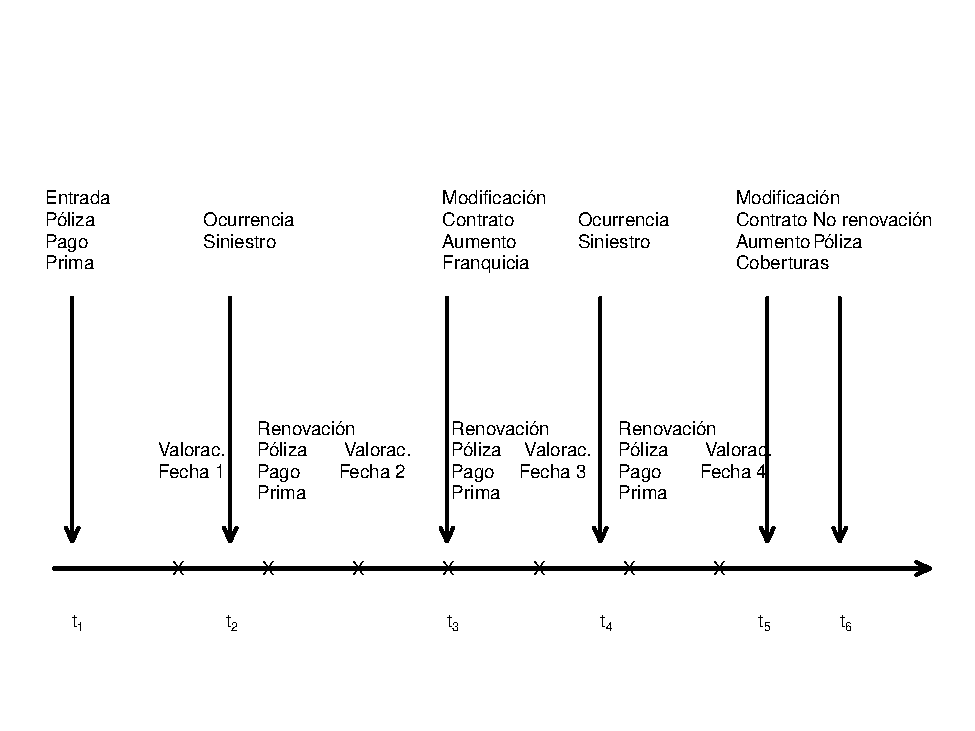
\includegraphics[width=1\linewidth]{LossDataAnalytics_files/figure-latex/StochOperations-1} 

}

\caption{Cronograma de una póliza de seguro estándar. Las flechas marcan las ocurrencias de eventos aleatorios. Cada x marca el instante de los eventos programados que normalmente no son aleatorios.}\label{fig:StochOperations}
\end{figure}

\hypertarget{S:PredModApps}{%
\section{Operaciones de la Compañía de Seguros}\label{S:PredModApps}}

\begin{center}\rule{0.5\linewidth}{0.5pt}\end{center}

En esta sección, se aprenderá a:

\begin{itemize}
\tightlist
\item
  Describir cinco áreas operativas principales de las compañías de seguros.
\item
  Identificar el papel de las oportunidades que aportan los datos y la analítica dentro de cada área operativa.
\end{itemize}

\begin{center}\rule{0.5\linewidth}{0.5pt}\end{center}

Usando los datos de seguros, el objetivo final es utilizar los datos para tomar decisiones. Aprenderemos más sobre métodos de análisis y extrapolación de datos en capítulos futuros. Para empezar, pensemos por qué queremos hacer el análisis.
Tomaremos el punto de vista de la compañía de seguros (no el de la persona asegurada) e introduciremos formas de cobrar dinero, pagarlo, administrar los costes y asegurarnos de que tengamos suficiente capital para cumplir con las obligaciones de un asegurador. El énfasis está en las operaciones específicas de seguros más que en las actividades comerciales generales como la publicidad, el marketing y la gestión de recursos humanos.

Específicamente, en muchas compañías de seguros, se acostumbra a agregar los procesos de seguros concretos en unidades operativas más grandes; muchas empresas utilizan varias áreas funcionales para segregar las actividades de los empleados y sus áreas de responsabilidad. Los actuarios, otros analistas financieros y los reguladores de seguros trabajan dentro de estas unidades y utilizan datos para las siguientes actividades:

\begin{enumerate}
\def\labelenumi{\arabic{enumi}.}
\tightlist
\item
  \textbf{Inicio del seguro}. En esta etapa, la empresa toma una decisión sobre si debe asumir o no un riesgo (la etapa de suscripción) y asigna una prima (o tarifa). El análisis de seguros tiene sus raíces actuariales en \emph{la elaboración de tarifas}, donde los analistas buscan determinar el precio correcto por el riesgo correcto.
\item
  \textbf{Renovación del seguro}. Muchos contratos, particularmente en seguros generales, tienen duraciones relativamente cortas, como 6 meses o un año. Aunque existe una expectativa implícita de que todos los contratos se renovarán, el asegurador tiene la oportunidad de rechazar la cobertura y ajustar la prima. También se utiliza la analítica en esta etapa de renovación de la póliza donde el objetivo es retener a los clientes rentables.
\item
  \textbf{Gestión de siniestros}. La analítica de datos se ha utilizado durante mucho tiempo para (1) detectar y prevenir el fraude en las reclamaciones sinestros, (2) administrar los costes de los siniestros, incluyendo el identificar el soporte adecuado para los gastos de tramitación de siniestros, así como (3) comprender los tramos de exceso de coste para fijar la retención y el reaseguro.
\item
  \textbf{Reserva de pérdidas}. Las herramientas analíticas se utilizan para proporcionar a los gestores una estimación adecuada de las obligaciones futuras y para cuantificar la incertidumbre de esas estimaciones.
\item
  \textbf{Solvencia y Asignación de Capital}. Decidir sobre el requisito de cantidad de capital y sobre las formas de asignar capital entre las inversiones alternativas también son actividades analíticas esenciales. Las empresas deben evaluar cuánto capital es necesario para tener un flujo de efectivo disponible suficiente para cumplir con sus obligaciones cuando llegue el momento de que se materialicen (solvencia). Esta es una pregunta importante que concierne no solo a los gerentes de la empresa, sino también a los clientes, los accionistas de la empresa, las autoridades reguladoras, así como a la sociedad en general. Relacionado con la cuestión de cuánto capital es necesario, hay que abordar la cuestión de cómo asignar ese capital a los diferentes proyectos financieros, por lo general para maximizar un retorno de la inversión. Aunque esta pregunta puede surgir a varios niveles, las compañías de seguros generalmente se preocupan por cómo asignar capital a sus diferentes líneas de negocio dentro de la empresa y a diferentes filiales de una misma empresa matriz.
\end{enumerate}

Aunque los datos representan un componente crítico para el cálculo del capital de solvencia y la asignación, otros componentes, incluido el marco económico local y global, el entorno de inversiones financieras y los requisitos específicos fijados por el entorno regulatorio del momento, también son importantes. Debido a los conocimientos previos requeridos para abordar estos temas, no abordaremos cuestiones de solvencia, asignación de capital y regulación en este texto.

No obstante, para todas las funciones operativas, enfatizamos que la analítica en la industria de seguros no es un ejercicio que un pequeño grupo de analistas pueden hacer por sí mismos. Requiere que una aseguradora realice importantes inversiones en tecnología de la información, marketing, suscripción, y funciones actuariales. Como estas áreas representan los principales objetivos finales del análisis de datos, en las siguientes subsecciones se presentan los antecedentes adicionales de cada unidad operativa.

\hypertarget{inicio-del-seguro}{%
\subsection{Inicio del seguro}\label{inicio-del-seguro}}

Fijar el precio de un producto de seguro puede ser un problema desconcertante. Ello contrasta con otras industrias, como la fabricación, donde el coste de un producto es (relativamente) conocido y proporciona un punto de referencia para evaluar un precio de demanda del mercado. De manera similar, en otras áreas de servicios financieros, los precios de mercado están disponibles y proporcionan la base para una estructura de precios de productos coherente con el mercado. Sin embargo, para muchas líneas de seguros, el coste de un producto es incierto y los precios de mercado no están disponibles. La esperanza del coste aleatorio es un razonable punto de partida para fijar un precio. (Si se ha estudiado finanzas, se recordará que una esperanza es el precio óptimo para una aseguradora neutral al riesgo). Ha sido tradicional en la fijación de precios de seguros empezar siempre con el coste esperado. Las aseguradoras luego agregan márgenes a este coste esperado, para tener en cuenta el riesgo del producto, los gastos incurridos en el mantenimiento del producto y una provisión para beneficios/excedentes de la empresa.

El uso de los costes esperados como base para la fijación de precios prevalece en algunas líneas del negocio de seguros como los seguros para propietarios de viviendas y los seguros de automóviles. Para estas tipologías, la analítica ha servido para mejora el precio que llega al mercado al hacer que el cálculo del coste esperado del producto sea más preciso. La creciente disponibilidad de Internet por parte de los consumidores también ha servido para aumentar la transparencia en los precios. En el mercado actual, los consumidores tienen fácil acceso a los precios ofertados por una gran cantidad de aseguradoras. Las aseguradoras buscan aumentar su cuota de mercado mediante el perfeccionamiento de sus sistemas de clasificación de riesgo, logrando así una mejor aproximación de precios en determinados productos y permitiendo estrategias de suscripción de los clientes óptimos (``cream-skimming'' es una frase que se utiliza cuando la aseguradora suscribe solo los mejores riesgos). Algunas encuestas recientes (por ejemplo, \citet{survey2013}) indican que la fijación de precios es el área donde más se usa la analítica en las aseguradoras.

\emph{Suscripción}, el proceso de clasificación de riesgos en categorías homogéneas y la asignación de asegurados a esas categorías, se encuentra en el núcleo de la elaboración de tarifas. Los asegurados de cada una de las clases (categorías) tienen un perfil de riesgo similar y, por lo tanto, se les cobra un mismo precio por el seguro que suscriben. Este es el concepto de prima actuarialmente justa; es justo cobrar tarifas diferentes si los asegurados muestran diferencias identificables en los factores de riesgo. En un artículo pionero, \emph{Two Studies in Automobile Insurance Ratemaking} \citep{bailey1960} proporcionó un catalizador para la aceptación de métodos analíticos en el sector de los seguros. Este trabajo abordaba el problema de la clasificación en tarificación. Describía un ejemplo de seguro de automóvil con cinco clases de clasificación cruzada por uso y cuatro tipos de bonificación relacionados con el mérito del asegurado. Hasta ese momento, la dependencia de las primas por uso y tipo de bonificación se determinaban por separado. Tener en cuenta la interacción de los efectos de las diferentes variables de clasificación es un problema más difícil de resolver.

\hypertarget{renovaciuxf3n-del-seguro}{%
\subsection{Renovación del seguro}\label{renovaciuxf3n-del-seguro}}

El seguro es un tipo de servicio financiero y, como muchos otros servicios o contratos, la cobertura del seguro a menudo se acuerda por un tiempo limitado, cuyo transcurso marca la finalización del compromiso de proporcionar cobertura. En particular para los seguros generales, la necesidad de cobertura continúa, por lo que se hace un esfuerzo para emitir un nuevo contrato que brinde una cobertura similar, cuando el contrato existente llega al final de su vigencia. A esto se le llama renovación de la póliza. También puede surgir la necesidad de renovación de las pólizas en los seguros de vida, por ejemplo, en el seguro de vida temporal. No sucede lo mismo en otros contratos, como en el seguro de rentas vitalicias, que termina con el fallecimiento del asegurado y, por lo tanto, en el que la cuestiones relativas a la renovación son irrelevantes.

En ausencia de restricciones legales, en la renovación, el asegurador tiene la oportunidad de:

\begin{itemize}
\tightlist
\item
  aceptar o negarse a suscribir el riesgo; y
\item
  determinar una nueva prima, posiblemente junto con una nueva clasificación del riesgo.
\end{itemize}

La clasificación y tarificación del riesgo en el momento de la renovación se basa en dos tipos de información. Primero, en la etapa inicial, el asegurador tiene muchas variables de calificación disponibles para poder tomar una decisión. Muchas variables no cambiarán posteriormente, por ejemplo el sexo, mientras que es probable que otras cambien, por ejemplo la edad, y otras pueden cambiar o no, por ejemplo, la valoración crediticia.
En segundo lugar, a diferencia de la etapa inicial, en la renovación, el asegurador tiene a su disposición un historial de la experiencia de las pérdidas sufridas por el titular de la póliza, y este historial puede proporcionar información sobre el asegurado que no estaba disponible en la tarificación mediante las variables iniciales. La modificación de primas con historial de siniestros se conoce como \emph{tarificación basada en la experiencia}, también conocida como \emph{tarificación por méritos}.

Los métodos de tarificación basada en la experiencia se aplican retrospectivamente o prospectivamente. Con los métodos retrospectivos, se proporciona al tomador de la póliza un reembolso de una parte de la prima si se dan de ciertas condiciones de experiencia favorable (para la aseguradora). Las primas retrospectivas son habituales en los acuerdos de seguros de vida (donde los asegurados ganan dividendos en los EE. UU., bonificaciones en el Reino Unido y participación en las ganancias en la cobertura de vida temporal en Israel). En los seguros generales, los métodos prospectivos son más frecuentes, y se recompensa la experiencia favorable del asegurado a través de una prima de renovación más baja.

El historial de siniestralidad puede proporcionar información sobre el apetito al riesgo del asegurado. Por ejemplo, en líneas personales se suele usar una variable para indicar si se ha producido o no un siniestro en los últimos tres años.
Otro ejemplo es el de una línea comercial como el seguro de empleo u ocupación, en el que se puede observar la frecuencia o gravedad promedio de las reclamaciones de siniestros de un asegurado durante los últimos tres años. El historial de siniestros puede revelar información que de otro modo estaría oculta (para la aseguradora) sobre el titular de la póliza.

\hypertarget{gestiuxf3n-de-productos-y-siniestros}{%
\subsection{Gestión de productos y siniestros}\label{gestiuxf3n-de-productos-y-siniestros}}

En algunas áreas de los seguros, el proceso de pago de reclamaciones para los siniestros que están cubiertos es relativamente sencillo. Por ejemplo, en los seguros de vida, un certificado de defunción simple es todo lo que se necesita para percibir la cuantía que corresponde al beneficiario tal como se estipule en el contrato. Sin embargo, en áreas no relacionadas con la vida como en los seguros de propiedad y accidentes, el proceso puede ser mucho más complejo. Pensemos por ejemplo en un suceso relativamente simple como un accidente de automóvil. Aquí, a menudo se requiere determinar qué parte tiene la culpa del accidente, es necesario evaluar los daños a todos los vehículos y personas involucrados en el siniestro, tanto asegurados como no asegurados, los gastos incurridos en la evaluación de los daños también deben evaluarse, y así sucesivamente. El proceso de determinación de cobertura, responsabilidad legal y resolución de reclamaciones se conoce como tramitación de siniestros.

Los aseguradores a veces usan el concepto de fuga o escape para referirse al dinero perdido en las ineficiencias de la gestión de siniestros. Hay muchas formas en las que la analítica de datos puede ayudar a gestionar el proceso de tramitación, \citet{SASsurvey}. Históricamente, la tarea más importante ha sido la detección de fraudes.
El proceso de tramitación de siniestros implica reducir la asimetría de información (el reclamante sabe lo que pasó; la empresa sabe sólo algo de lo que pasó). Mitigar el fraude es una parte importante del proceso de gestión de siniestros.

La detección de fraudes es solo un aspecto de la gestión de las reclamaciones. En términos más generales, se puede pensar que la gestión de siniestros consta de los siguientes componentes:

\textbf{Triaje de siniestros}. Al igual que en el mundo médico, la identificación precoz y el manejo apropiado de los siniestros de elevada cuantía (pacientes, en el mundo médico), puede conducir a ahorros substanciales. Por ejemplo, en los seguros de empleo, las aseguradoras buscan lograr la identificación temprana de aquellos siniestros que corren el riesgo de incurrir en elevados costes médicos y un largo período de pago. La intervención temprana en estos casos podría dar a las aseguradoras un mayor control sobre la gestión del siniestro, el tratamiento médico y los costes generales para lograr un retorno al trabajo lo más pronto posible.

\textbf{Tramitación de siniestros}. El objetivo es utilizar la analítica para identificar siniestros muy habituales que se prevé que tendrán un coste pequeño. Las situaciones más complejas pueden requerir peritos más experimentados y asistencia legal para manejar adecuadamente las reclamaciones con un coste potencial elevado.

\textbf{Decisiones de peritaje}. Una vez se identifica un siniestro complejo y se asigna a un perito, se pueden establecer rutinas analíticas para ayudar a los procesos posteriores de toma de decisiones. Dichos procesos también pueden ser útiles para los peritos en el cálculo reservas, una estimación de la responsabilidad futura del asegurador. Esta es una información importante para calcular las reservas por pérdidas de la aseguradora, descritas en la Sección \ref{S:Reserving}.

Además del reembolso de las pérdidas que satisface el asegurador, éste también debe preocuparse por otra fuente de pérdida de ingresos, los gastos. Los gastos de peritaje de las pérdidas son parte del coste de gestión de los siniestros de una aseguradora. La analítica de datos se puede utilizar para reducir gastos directamente relacionados con la gestión de siniestros (asignados) así como el tiempo del personal que en general se usa para supervisar los procesos de gestión de los siniestros (no asignados). El sector asegurador tiene costes operativos elevados en relación con otras organizaciones del sector de los servicios financieros.

Además de los pagos de las reclamaciones, hay muchas otras formas en las que las aseguradoras utilizan datos para gestionar sus productos. Ya hemos discutido la necesidad de analizar la suscripción, es decir, la clasificación de los riesgos en las etapas iniciales de adquisición y renovación. Las aseguradoras también están interesadas en qué tipo de asegurados deciden renovar su contrato y, al igual que con otros productos, están interesadas en monitorizar la fidelidad de sus clientes.

La analítica también se puede utilizar para gestionar una cartera de pólizas o el conjunto de riesgos que ha suscrito una aseguradora. Cuando se presenta inicialmente el riesgo, la aseguradora puede actuar imponiendo parámetros contractuales que modifiquen las condiciones ligadas a los pagos que prevé el contrato. Los capítulos \ref{C:Severity} y \ref{C:PortMgt} describen las modificaciones más usuales que incluyen el coaseguro, las franquicias y los límites superiores de la póliza.

Una vez acordados los términos del contrato con un asegurado, el asegurador puede todavía modificar su obligación neta mediante la celebración de un convenio de reaseguro. Este tipo de contrato se realiza con un reasegurador, un asegurador de un asegurador. Es completamente normal que las compañías de seguros adquieran seguros para su cartera de riesgos a fin de obtener protección contra sucesos inusuales, al igual que las personas y otras empresas lo hacen.

\hypertarget{S:Reserving}{%
\subsection{Provisiones}\label{S:Reserving}}

Una característica importante que distingue a los seguros de otros sectores de la economía es el momento del intercambio de los bienes. En la industria manufacturera, los pagos por bienes generalmente se realizan en el momento de una transacción. Por el contrario, en el caso de los seguros, el dinero recibido de un cliente se obtiene antes de los beneficios o servicios; estos se concretan en una fecha posterior, en la que ocurre el hecho asegurado. Esto lleva a la necesidad de disponer de una reserva de capital para hacer frente a las obligaciones futuras respecto de las obligaciones asumidas y para ganarse la confianza de los asegurados respecto a que la empresa podrá cumplir con sus compromisos. El tamaño de esta reserva de capital y la importancia de garantizar su adecuación es una de las principales preocupaciones de la industria de seguros.

La reserva de capital para siniestros impagados se conoce como reserva por pérdidas; en algunas jurisdicciones, las reservas también se conocen como \emph{provisiones técnicas}. En la Figura \ref{fig:StochOperations} se aprecia las veces en las que una empresa cierra su posición financiera; estos momentos se conocen como fechas de valoración.
Los siniestros que se declaran antes de las fechas de valoración normalmente ya se han pagado, están en proceso de pago o están a punto de pagarse; Se desconocen los siniestros que se devengarán tras las fechas de valoración. Una empresa debe estimar estos pasivos pendientes al determinar su solidez financiera. Determinar con precisión las provisiones es importante para las aseguradoras por muchas razones.

\begin{enumerate}
\def\labelenumi{\arabic{enumi}.}
\tightlist
\item
  Las provisiones representan una reclamación anticipada que la aseguradora debe a sus clientes.
  Una provisión insuficiente puede acabar en un incumplimiento de las responsabilidades de la reclamación de un siniestro. Por el contrario, una aseguradora con excesivas provisiones puede presentar una peor posición financiera de la que realmente tiene.
\item
  Las provisiones proporcionan una estimación del coste no pagado del seguro que se pueden utilizar para calcular precios de nuevos contratos.
\item
  Las leyes y regulaciones exigen el establecimiento de provisiones. La sociedad tiene sumo interés en que se pueda garantizar la solidez financiera y la solvencia de las aseguradoras.
\item
  Además de la administración y los reguladores de las compañías de seguros, otras partes interesadas, como inversores y clientes, toman decisiones que dependen de las provisiones que tenga una empresa.
\end{enumerate}

Las provisiones son un área del seguro en la que existen diferencias sustanciales entre los seguros de vida y los seguros generales (también conocido como no-vida). En los seguros de vida, la gravedad (cuantía de la pérdida) a menudo no es una fuente de incertidumbre ya que los pagos a realizar se especifican en el contrato. La frecuencia, determinada por la curva de mortalidad de los asegurados, es lo que preocupa. Sin embargo, debido a la cantidad de tiempo que transcurre hasta la liquidación de los contratos de seguros de vida, el valor temporal de la incertidumbre monetaria medida desde la emisión hasta la fecha de pago puede dominar las preocupaciones sobre la frecuencia. Por ejemplo, para un asegurado que compra un contrato de vida a los 20 años, no sería raro que el contrato siguiera abierto al cabo de 60 años, cuando el asegurado celebrase su 80 cumpleaños. Para más información, ver, por ejemplo, \citet{bowers1986actuarial} o \citet{dickson2013actuarial} para obtener información sobre cómo reservar un seguro de vida.

\hypertarget{S:LGPIF}{%
\section{Caso de Estudio: Fondo de Propiedad de Wisconsin}\label{S:LGPIF}}

\begin{center}\rule{0.5\linewidth}{0.5pt}\end{center}

En esta sección, usamos el Fondo de Propiedad de Wisconsin como un caso de estudio. Se aprenderá a:

\begin{itemize}
\tightlist
\item
  Describir cómo los sucesos que generan la información pueden producir datos de interés para los analistas de seguros.
\item
  Producir estadísticas descriptivas relevantes para cada variable.
\item
  Describir cómo se pueden utilizar estos resultados en cada una de las principales áreas operativas de una compañía de seguros.
\end{itemize}

\begin{center}\rule{0.5\linewidth}{0.5pt}\end{center}

Ilustremos el tipo de datos bajo consideración y los objetivos que deseamos lograr mediante el análisis de la Local Government Property Insurance Fund (LGPIF), un conjunto de pólizas de seguros administrado por la Oficina del Comisionado de Seguros de Wisconsin. La LGPIF se creó para proporcionar seguros de propiedad para entidades gubernamentales locales que incluían condados, ciudades, pueblos, aldeas, distritos escolares y de bibliotecas.
El fondo asegura toda propiedad del gobierno local, como los edificios gubernamentales, las escuelas, las bibliotecas y los vehículos de motor. El fondo cubre toda pérdida que afecta a la propiedad, excepto las que son consecuencia de inundaciones, terremotos, desgaste,
temperaturas extremas, moho, guerras, reacciones nucleares y malversación de fondos o robo por parte de un empleado.

El fondo cubre más de mil entidades gubernamentales locales que pagan aproximadamente 25 millones de dólares en primas cada año y reciben una cobertura de seguro de aproximadamente 75 mil millones de dólares. Los edificios del gobierno estatal no están cubiertos; la LGPIF es para entidades del gobierno local que tienen responsabilidades presupuestarias separadas y que necesitan un seguro para moderar los efectos presupuestarios de sucesos asegurables inciertos. La cobertura a la propiedad del gobierno local ha estado vigente en Wisconsin desde 1911, proporcionando así una gran cantidad de datos históricos.

En esta ilustración, restringimos el análisis a los siniestros de la cobertura de los edificios y su contenido; no consideramos siniestros de vehículos motorizados y equipos especializados que son propiedad de las entidades locales (como máquinas quitanieves). También consideramos solo las reclamaciones que están cerradas, con obligaciones totalmente cumplidas.

\hypertarget{S:OutComes}{%
\subsection{Variables de siniestralidad del fondo: frecuencia y severidad}\label{S:OutComes}}

Fundamentalmente, las compañías de seguros aceptan primas a cambio de promesas de compensar al asegurado en caso de que ocurra un siniestro contemplado en la póliza. La indemnización es la compensación proporcionada por la aseguradora por los daños, pérdidas o daños incurridos que están cubiertos por la póliza. Esta compensación también se conoce como \emph{siniestro}. La magnitud de la cuantía del pago, conocido como \emph{severidad}, es un gasto financiero clave para una aseguradora.

En términos de gasto monetario, a una aseguradora le es indiferente tener diez siniestros de 100 que un siniestro de 1000. No obstante, es habitual que las aseguradoras estudien la frecuencia con la que se producen los siniestros, conocida como la \emph{frecuencia} de siniestralidad. La frecuencia es importante para calcular los gastos, pero también influye en la determinación de los parámetros contractuales (como la franquicia y los límites de la póliza que se describen más adelante) que se establecen en función de la ocurrencia concreta de cada siniestro y se va controlando periódicamente por el supervisor de los seguros, y puede ser un factor clave en la determinación del compromiso de indemnización global del asegurador. Consideraremos la frecuencia y la severidad como las dos principales variables de siniestralidad que deseamos comprender, modelar y gestionar.

Por ejemplo, en 2010 había 1.110 asegurados en el fondo de propiedad que sufrieron un total de 1.377 siniestros. La tabla \ref{tab:Frequency2010} muestra la distribución. Casi dos tercios (0,637) de los asegurados no tuvieron ningún siniestro y un 18,8\% adicional tuvo solo un siniestro. El 17,5\% restante (= 1-0,637-0,188) tuvo más de un siniestro; el asegurado con el mayor número de siniestros registró un total de 239. El número medio de siniestros en esta muestra fue 1,24 (= 1377/1110).

\begin{longtable}[]{@{}llllllllllll@{}}
\caption{\label{tab:Frequency2010} 2010 Distribución de frecuencia de los siniestros}\tabularnewline
\toprule
Tipo & & & & & & & & & & & \\
\midrule
\endfirsthead
\toprule
Tipo & & & & & & & & & & & \\
\midrule
\endhead
Número & 0 & 1 & 2 & 3 & 4 & 5 & 6 & 7 & 8 & 9 o más & Suma \\
Frec. & 707 & 209 & 86 & 40 & 18 & 12 & 9 & 4 & 6 & 19 & 1110 \\
Siniestros & 0 & 209 & 172 & 120 & 72 & 60 & 54 & 28 & 48 & 617 & 1377 \\
Proporción & 0,637 & 0,188 & 0,077 & 0,036 & 0,016 & 0,011 & 0,008 & 0,004 & 0,005 & 0,017 & 1,000 \\
\bottomrule
\end{longtable}

Para analizar la distribución de la severidad, el enfoque habitual es examinar la distribución de la muestra de los 1.377 siniestros. Sin embargo, otra alternativa consiste en examinar la distribución del promedio de los siniestros de los asegurados que sufrieron algún siniestro. En nuestra muestra de 2010, hubo 403 (= 1110-707) asegurados que sufrieron algún siniestro. Para 209 de dichos asegurados con un solo siniestro, el coste medio es igual al coste del único siniestro que tuvieron. Para el asegurado con mayor frecuencia, el coste medio es un promedio de 239 siniestros declarados por separado. Este promedio también se conoce como la prima pura o \emph{coste del siniestro}.

La tabla \ref{tab:Severity2010} resume la distribución de la muestra de las severidades promedio de los 403 asegurados que presentaron una reclamación de siniestro; muestra que el coste medio los siniestros fue igual a 56.330 (todos los costes están expresados en dólares estadounidenses). Sin embargo, el promedio solo da una mirada limitada de la distribución. Se puede extraer más información de los estadísticos descriptivos resumen que muestran un siniestro muy grande con una cuantía igual a 12.920.000. La figura \ref{fig:SeverityFig} proporciona más información sobre la distribución del coste de los siniestros de la muestra, y revela una distribución que está dominada por este único gran siniestro de modo que el histograma no es muy útil. Incluso al eliminar el siniestro elevado, nos encontramos ante una distribución que está sesgada a la derecha. En general, la técnica más aceptada es trabajar con severidades expresadas en unidades logarítmicas, especialmente cuando se analizan gráficos; la figura correspondiente en el panel de la derecha es mucho más fácil de interpretar.

\begin{longtable}[]{@{}
  >{\raggedleft\arraybackslash}p{(\columnwidth - 10\tabcolsep) * \real{0.14}}
  >{\raggedleft\arraybackslash}p{(\columnwidth - 10\tabcolsep) * \real{0.15}}
  >{\raggedleft\arraybackslash}p{(\columnwidth - 10\tabcolsep) * \real{0.12}}
  >{\raggedleft\arraybackslash}p{(\columnwidth - 10\tabcolsep) * \real{0.12}}
  >{\raggedleft\arraybackslash}p{(\columnwidth - 10\tabcolsep) * \real{0.15}}
  >{\raggedleft\arraybackslash}p{(\columnwidth - 10\tabcolsep) * \real{0.18}}@{}}
\caption{\label{tab:Severity2010} Distribución de la severidad promedio en 2010}\tabularnewline
\toprule
Mínimo & Primer
Cuartil & Mediana & Media & Tercer
Cuartil & Máximo \\
\midrule
\endfirsthead
\toprule
Mínimo & Primer
Cuartil & Mediana & Media & Tercer
Cuartil & Máximo \\
\midrule
\endhead
167 & 2.226 & 4.951 & 56.330 & 11.900 & 12.920.000 \\
\bottomrule
\end{longtable}

\begin{figure}

{\centering 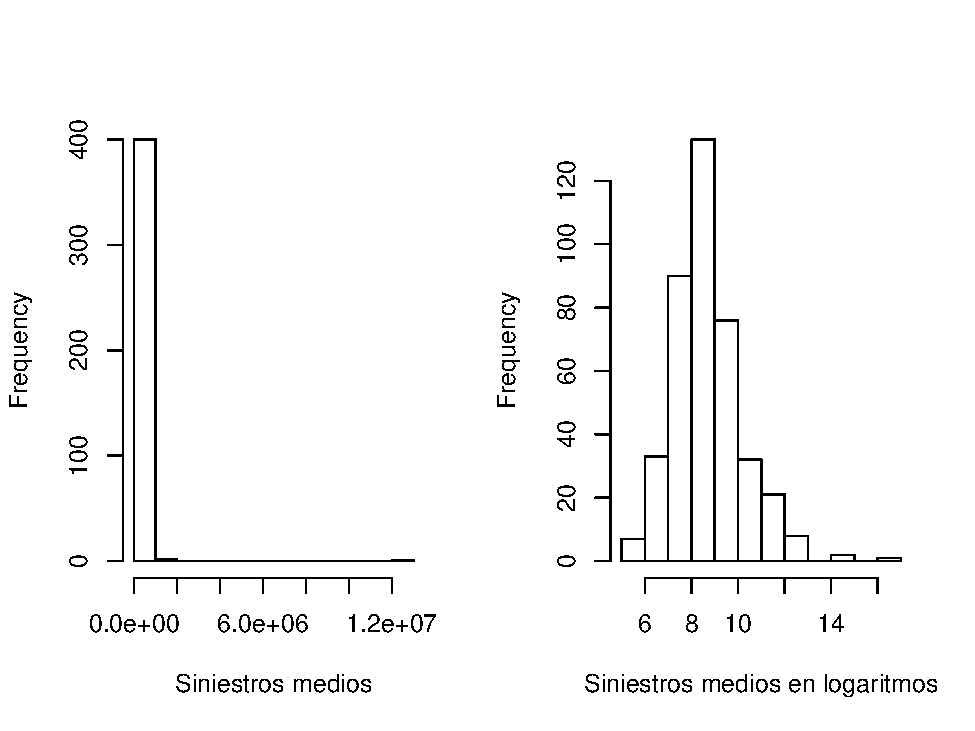
\includegraphics[width=0.8\linewidth]{LossDataAnalytics_files/figure-latex/SeverityFig-1} 

}

\caption{Distribución del promedio de severidades positivas}\label{fig:SeverityFig}
\end{figure}

\hypertarget{S:FundVariables}{%
\subsection{Variables de clasificación del fondo}\label{S:FundVariables}}

El objetivo de los primeros capítulos de este texto es desarrollar modelos para representar y gestionar las dos variables principales en el análisis de la siniestralidad, frecuencia y severidad.
Sin embargo, cuando los actuarios y otros analistas financieros utilizan esos modelos, lo hacen usando variables externas. En general, usando terminología estadística, se podría llamar a dichas variables las variables explicativas o predictoras; hay muchos otros nombres en estadística, economía, psicología y otras disciplinas. Debido a nuestro enfoque en seguros, vamos a llamarlas variables de tarificación ya que serán útiles para establecer tarifas y primas de seguros.

Habíamos empezado considerando las observaciones de una muestra de 1.110 asegurados que, en principio, podían parecer muchos. Sin embargo, como veremos en nuestras próximas aplicaciones, debido a la elevada presencia de ceros y a la elevada asimetría en los siniestros, los actuarios normalmente desean tener más datos. Un enfoque muy habitual, que adoptamos aquí, es examinar los resultados de varios años, aumentando así el tamaño de la muestra. Discutiremos las fortalezas y limitaciones de esta estrategia más adelante, pero, de momento, solo vamos a explicar al lector cómo funciona.

Específicamente, la Tabla \ref{tab:CoverageBCIM} muestra que ahora consideramos pólizas vigentes en cinco años con datos disponibles, 2006, \ldots, 2010, incluido. Los datos comienzan en 2006 porque hubo un cambio en la codificación de los siniestros en 2005, por lo que no es posible realizar comparaciones con años anteriores. Para mitigar el efecto de los siniestros abiertos, sólo consideraremos los años anteriores a 2011. Un siniestro abierto significa que todavía no se conocen todas las obligaciones que implica dicho siniestro en el momento del análisis; para algunos siniestros, como cuando existe una lesión a una persona en un accidente de automóvil o en el lugar de trabajo, se sabe que pueden pasar años antes de que los costes sean completamente conocidos.

\begin{longtable}[]{@{}
  >{\raggedright\arraybackslash}p{(\columnwidth - 8\tabcolsep) * \real{0.19}}
  >{\raggedleft\arraybackslash}p{(\columnwidth - 8\tabcolsep) * \real{0.17}}
  >{\raggedright\arraybackslash}p{(\columnwidth - 8\tabcolsep) * \real{0.19}}
  >{\raggedleft\arraybackslash}p{(\columnwidth - 8\tabcolsep) * \real{0.18}}
  >{\raggedleft\arraybackslash}p{(\columnwidth - 8\tabcolsep) * \real{0.19}}@{}}
\caption{\label{tab:CoverageBCIM} Resumen de siniestralidad por póliza}\tabularnewline
\toprule
Año & Promedio
Frecuenc. & Promedio
Severid. & Promedio
Coberturas & Número de
Asegurados \\
\midrule
\endfirsthead
\toprule
Año & Promedio
Frecuenc. & Promedio
Severid. & Promedio
Coberturas & Número de
Asegurados \\
\midrule
\endhead
2006 & 0,951 & 9.695 & 32.498.186 & 1.154 \\
2007 & 1,167 & 6.544 & 35.275.949 & 1.138 \\
2008 & 0,974 & 5.311 & 37.267.485 & 1.125 \\
2009 & 1,219 & 4.572 & 40.355.382 & 1.112 \\
2010 & 1,241 & 20.452 & 41.242.070 & 1.110 \\
\bottomrule
\end{longtable}

La tabla \ref{tab:CoverageBCIM} muestra que el siniestro medio varía a lo largo del tiempo, especialmente con un valor alto en el año 2010 (que vimos que estaba provocado por un único siniestro elevado) \footnote{Notemos que la severidad promedio en la Tabla \ref{tab:CoverageBCIM} difiere de la que se presenta en la Tabla \ref{tab:Severity2010}. Esto ocurre porque en la primera se incluyen las pólizas que no han tenido siniestros mientras que en esta última los excluye. Esta es una distinción importante que se tratará en algunos apartados posteriores del texto.}. El número total de asegurados va disminuyendo progresivamente y, por el contrario, la cobertura va aumentando. La variable de cobertura es la cantidad de cobertura de la propiedad y de los contenidos. Aproximadamente, se puede entender como el pago máximo posible que podría llegar a pagar el asegurador. Para nuestros propósitos inmediatos, la cobertura es nuestra primera variable de tarificación. En igualdad de condiciones, lo que esperamos es que titulares de pólizas con mayor cobertura tengan siniestros de coste más elevado.
Concretaremos mucho más esta idea a medida que avancemos en nuestro análisis, y también justificaremos esta expectativa a través de los datos.

Para tener una visión diferente de los datos de 2006-2010, la table \ref{tab:DeductCov} resume la distribución de nuestros dos resultados, frecuencia y coste del siniestro. En cada caso, el promedio excede la mediana, lo que sugiere que las dos distribuciones tienen asimetría a la derecha. Además, la table resume nuestras variables continuas de tarificación, cuantía de la cobertura y de la franquicia. La tabla muestra que estas variables también tienen distribuciones asimétricas a la derecha.

\begin{longtable}[]{@{}
  >{\raggedright\arraybackslash}p{(\columnwidth - 8\tabcolsep) * \real{0.26}}
  >{\raggedleft\arraybackslash}p{(\columnwidth - 8\tabcolsep) * \real{0.14}}
  >{\raggedleft\arraybackslash}p{(\columnwidth - 8\tabcolsep) * \real{0.12}}
  >{\raggedleft\arraybackslash}p{(\columnwidth - 8\tabcolsep) * \real{0.14}}
  >{\raggedleft\arraybackslash}p{(\columnwidth - 8\tabcolsep) * \real{0.18}}@{}}
\caption{\label{tab:DeductCov} Resumen de la frecuencia y coste de siniestros, franquicia y coberturas}\tabularnewline
\toprule
& Mínimo & Mediana & Media & Máximo \\
\midrule
\endfirsthead
\toprule
& Mínimo & Mediana & Media & Máximo \\
\midrule
\endhead
Frecuencia & 0 & 0 & 1,109 & 263 \\
Severidad & 0 & 0 & 9.292 & 12.922.218 \\
Franquicia & 500 & 1.000 & 3.365 & 100.000 \\
Cobertura (miles) & 8,937 & 11.354 & 37.281 & 2.444.797 \\
\bottomrule
\end{longtable}

El siguiente gráfico describe las variables de tarificación consideradas en este capítulo. Lo que deseamos que ocurra es que estas variables estén relacionadas de forma natural con la siniestralidad. Se puede obtener más información sobre dichas variables en \citet{frees2016multivariate}. Para eliminar a asimetría, de ahora en adelante nos centraremos en las transformaciones logarítmicas de coberturas y franquicias.

** Descripción de las variables de tarificación **

\[
{\small \begin{matrix}
\begin{array}{ l | l}
\hline
Variable    & Descripción \\
\hline
\text{EntityType}   & \text{Variable cualitativa que toma uno de los seis valores siguientes:  (Village, City,} \\
& ~~~~ \text{County, Misc, School, or Town)} \\
\text{LnCoverage}   & \text{Total de cobertura del continente (edificio) y contenido, en logaritmo de millones de dólares}\\
\text{LnDeduct}     & \text{Franquicia, en logaritmo de dólares} \\
\text{AlarmCredit}  & \text{ Variable cualitativa que toma uno de los cuatro valores siguientes:    (0, 5, 10, o 15)} \\
 &  ~~~~   \text{para alarmas de humo en habitación principal} \\
\text{NoClaimCredit}    & \text{Variable binaria que indica ausencia de siniestros en los dos años anteriores} \\
\text{Fire5 }           & \text{Variable binaria que indica que la categoría de incendios está por debajo de 5} \\
& ~~~~ \text{(El rango de las categorías de incendios va de 0 a 10)} \\
\hline
\end{array}
\end{matrix}}
\]

Para tener una idea de la relación entre las variables de tarificación no continuas y los siniestros, la Tabla \ref{tab:ClaimRateVar} presenta los resultados de siniestralidad cruzados con dichas variables categóricas. La Tabla \ref{tab:ClaimRateVar} muestra una variación sustancial en la frecuencia de siniestros y su severidad media según el tipo de entidad. También se observa mayor frecuencia y gravedad según la variable \({\tt Fire5}\) variable y lo contrario para la variable \({\tt NoClaimCredit}\). La relación obtenida para la variable \({\tt Fire5}\) es contraintuitiva, ya que se esperarían cuantías más bajas para los asegurados en áreas con mejor protección pública (cuando el código de protección es cinco o menos). Naturalmente, existen otras variables que influyen en esta relación. En seguida veremos cómo afectan otras variables del fondo en el análisis de regresión multivariante, donde hallaremos un signo intuitivo y convincente (negativo) para el efecto de la variable \({\tt Fire5}\).

\begin{longtable}[]{@{}
  >{\raggedright\arraybackslash}p{(\columnwidth - 6\tabcolsep) * \real{0.31}}
  >{\raggedleft\arraybackslash}p{(\columnwidth - 6\tabcolsep) * \real{0.17}}
  >{\raggedleft\arraybackslash}p{(\columnwidth - 6\tabcolsep) * \real{0.17}}
  >{\raggedleft\arraybackslash}p{(\columnwidth - 6\tabcolsep) * \real{0.17}}@{}}
\caption{\label{tab:ClaimRateVar} Resumen de siniestralidad según el tipo de entidad, la clase de incendio y la puntuación por ausencia de siniestros}\tabularnewline
\toprule
Variable & Número de
Pólizas & Frecuencia
Siniestros & Coste
Medio \\
\midrule
\endfirsthead
\toprule
Variable & Número de
Pólizas & Frecuencia
Siniestros & Coste
Medio \\
\midrule
\endhead
\emph{EntityType} & & & \\
Village & 1.341 & 0,452 & 10.645 \\
City & 793 & 1,941 & 16.924 \\
County & 328 & 4,899 & 15.453 \\
Misc & 609 & 0,186 & 43.036 \\
School & 1.597 & 1,434 & 64.346 \\
Town & 971 & 0,103 & 19.831 \\
\emph{Fire} & & & \\
Fire5=0 & 2.508 & 0,502 & 13.935 \\
Fire5=1 & 3.131 & 1,596 & 41.421 \\
\emph{No Claims Credit} & & & \\
NoClaimCredit=0 & 3.786 & 1,501 & 31.365 \\
NoClaimCredit=1 & 1.853 & 0,310 & 30.499 \\
\textbf{Total} & 5.639 & 1,109 & 31.206 \\
\bottomrule
\end{longtable}

La tabla \ref{tab:RateAlarmCredit} muestra la experiencia de siniestralidad según la puntuación de alarma.
Se demuestra la dificultad de examinar las variables individualmente.
Por ejemplo, cuando miramos la experiencia de todas las entidades, vemos que los titulares de pólizas sin puntuación de alarma tienen un coste medio de siniestros y una frecuencia más baja que los asegurados con mayor puntuación de alarma (un 15\% de los asegurados cuentan con sistemas de vigilancia las 24h a través de una estación de bomberos o empresa de seguridad). En particular, cuando miramos el tipo de entidad ``School'', la frecuencia es 0,422 y la severidad 25.523 si no hay puntuación de alarma, mientras que para el nivel de alarma más alto los valores ascienden a 2,008 y 85.140, respectivamente. Esto puede significar simplemente que las entidades con más siniestros son las que probablemente tengan tendencia a poner un sistema de alarma. En resumen, las tablas no examinan los efectos multivariantes; por ejemplo, la tabla \ref{tab:ClaimRateVar} ignora cómo el efecto del tamaño (las cuantía de cobertura) afecta a la siniestralidad.

\begin{longtable}[]{@{}
  >{\raggedright\arraybackslash}p{(\columnwidth - 12\tabcolsep) * \real{0.12}}
  >{\raggedleft\arraybackslash}p{(\columnwidth - 12\tabcolsep) * \real{0.15}}
  >{\raggedleft\arraybackslash}p{(\columnwidth - 12\tabcolsep) * \real{0.14}}
  >{\raggedleft\arraybackslash}p{(\columnwidth - 12\tabcolsep) * \real{0.14}}
  >{\raggedleft\arraybackslash}p{(\columnwidth - 12\tabcolsep) * \real{0.15}}
  >{\raggedleft\arraybackslash}p{(\columnwidth - 12\tabcolsep) * \real{0.14}}
  >{\raggedleft\arraybackslash}p{(\columnwidth - 12\tabcolsep) * \real{0.14}}@{}}
\caption{\label{tab:RateAlarmCredit} Resumen la siniestralidad según el tipo de entidad y la categoría de puntuación de alarma (AC)}\tabularnewline
\toprule
Entidad
Tipo & AC0
Sini.
Frecuencia & AC0
Pro.
Severidad & AC0
Núm.
Pólizas & AC5
Sini.
Frecuencia & AC5
Pro.
Severidad & AC5
Núm.
Polizas \\
\midrule
\endfirsthead
\toprule
Entidad
Tipo & AC0
Sini.
Frecuencia & AC0
Pro.
Severidad & AC0
Núm.
Pólizas & AC5
Sini.
Frecuencia & AC5
Pro.
Severidad & AC5
Núm.
Polizas \\
\midrule
\endhead
Village & 0,326 & 11.078 & 829 & 0,278 & 8.086 & 54 \\
City & 0,893 & 7.576 & 244 & 2,077 & 4.150 & 13 \\
County & 2,140 & 16.013 & 50 & - & - & 1 \\
Misc & 0,117 & 15.122 & 386 & 0,278 & 13.064 & 18 \\
School & 0,422 & 25.523 & 294 & 0,410 & 14.575 & 122 \\
Town & 0,083 & 25.257 & 808 & 0,194 & 3.937 & 31 \\
Total & 0,318 & 15.118 & 2.611 & 0,431 & 10.762 & 239 \\
\bottomrule
\end{longtable}

\begin{longtable}[]{@{}
  >{\raggedright\arraybackslash}p{(\columnwidth - 12\tabcolsep) * \real{0.12}}
  >{\raggedright\arraybackslash}p{(\columnwidth - 12\tabcolsep) * \real{0.15}}
  >{\centering\arraybackslash}p{(\columnwidth - 12\tabcolsep) * \real{0.14}}
  >{\centering\arraybackslash}p{(\columnwidth - 12\tabcolsep) * \real{0.14}}
  >{\raggedleft\arraybackslash}p{(\columnwidth - 12\tabcolsep) * \real{0.15}}
  >{\raggedleft\arraybackslash}p{(\columnwidth - 12\tabcolsep) * \real{0.14}}
  >{\raggedleft\arraybackslash}p{(\columnwidth - 12\tabcolsep) * \real{0.14}}@{}}
\caption{Resumen de la siniestralidad según el tipo de entidad y la categoría de puntuación de alarma (AC)}\tabularnewline
\toprule
Entidad
Tipo & AC10
Sini.
Frequencia & AC10
Pro.
Severidad & AC10
Núm.
Pólizas & AC15
Sini.
Frequencia & AC15
Pro.
Severidad & AC15
Núm.
Pólizas \\
\midrule
\endfirsthead
\toprule
Entidad
Tipo & AC10
Sini.
Frequencia & AC10
Pro.
Severidad & AC10
Núm.
Pólizas & AC15
Sini.
Frequencia & AC15
Pro.
Severidad & AC15
Núm.
Pólizas \\
\midrule
\endhead
Village & 0,500 & 8.792 & 50 & 0,725 & 10.544 & 408 \\
City & 1,258 & 8.625 & 31 & 2,485 & 20.470 & 505 \\
County & 2,125 & 11.688 & 8 & 5,513 & 15.476 & 269 \\
Misc & 0,077 & 3.923 & 26 & 0,341 & 87.021 & 179 \\
School & 0,488 & 11.597 & 168 & 2,008 & 85.140 & 1,013 \\
Town & 0,091 & 2.338 & 44 & 0,261 & 9.490 & 88 \\
Total & 0,517 & 10.194 & 327 & 2,093 & 41.458 & 2.462 \\
\bottomrule
\end{longtable}

\hypertarget{operativa-del-fondo}{%
\subsection{Operativa del fondo}\label{operativa-del-fondo}}

Hasta ahora hemos visto las dos variables de siniestralidad del Fondo: una variable de recuento para el número de siniestros y una variable continua para el coste de las reclamaciones. También hemos introducido una variable de tarificación continua (cobertura); una variable cuantitativa discreta (franquicia en logarítmicos); dos variables de tarificación binarias (ausencia de siniestralidad y clase de incendio); y dos variables de tarificación categóricas (tipo de entidad y crédito de alarma). En los capítulos siguientes se explica cómo analizar y modelizar la distribución de dichas variables y sus relaciones. Antes de entrar en los detalles técnicos, pensemos a dónde queremos llegar. Las áreas funcionales de una compañía de seguros se describen en la Sección \ref{S:PredModApps}; veamos ahora cómo se aplicarían dichas áreas al contexto del fondo de propiedad que estamos analizando.

\hypertarget{inicio-del-seguro-1}{%
\subsubsection*{Inicio del seguro}\label{inicio-del-seguro-1}}
\addcontentsline{toc}{subsubsection}{Inicio del seguro}

Debido a que este es un fondo patrocinado por el gobierno, no tenemos que preocuparnos por seleccionar buenos riesgos o evitar malos riesgos; al fondo no se le permite denegar una solicitud de cobertura de una entidad gubernamental local. Por lo tanto, si no existe un proceso de suscripción, ¿qué hay que cobrar?

Podríamos mirar la experiencia más reciente en 2010, donde el total de todos los siniestros del fondos alcanzó la cifra de 28,16 millones de USD (\(= 1377 \text{ siniestros} \times 20452 \text{ coste medio}\)). Si lo dividimos entre
1.110 asegurados, eso sugiere una prima igual a 24.370 (\(\approx\) 28.160.000/1110). Sin embargo, 2010 fue un mal año; usando el mismo método, nuestra prima sería mucho menor según los datos de 2009. Este vaivén de las primas frustraría el propósito principal del fondo, que no es otro que fijar un precio constante que los administradores de propiedades locales puedan utilizar en sus presupuestos.

Tener un precio único para todos los asegurados es bueno, pero difícilmente parece justo. Por ejemplo, la tabla \ref{tab:ClaimRateVar} sugiere que las escuelas tienen siniestros mucho más costosos que otras entidades y, por lo tanto, deberían pagar más. Sin embargo, hacer el cálculo entidad por entidad tampoco sería lo correcto. Por ejemplo, como vimos en la tabla \ref{tab:RateAlarmCredit} aquellas entidades con una puntuación de alarma del 15\% (con un buen comportamiento, al tener los mejores sistemas de alarma) en realidad terminarían pagando más.

Entonces, parece que tenemos los datos para calcular primas adecuadas pero hay que profundizar en el análisis. Exploraremos estos aspectos más adelante en el Capítulo \ref{C:PremiumFoundations} sobre \emph{fundamentos de cálculo de primas}.
La selección de riesgos se introduce en el Capítulo \ref{C:RiskClass} sobre \emph{clasificación de riesgos}.

\hypertarget{renovaciuxf3n-del-seguro-1}{%
\subsubsection*{Renovación del seguro}\label{renovaciuxf3n-del-seguro-1}}
\addcontentsline{toc}{subsubsection}{Renovación del seguro}

Aunque el seguro de propiedad es típicamente un contrato de un año, la Table \ref{tab:CoverageBCIM} sugiere que los asegurados tienden a renovar; esto es lo más habitual en los seguros generales. Para renovar a los asegurados, además de sus variables de tarificación, tenemos su historial de siniestralidad, que puede ser un buen predictor de los siniestros que van a producirse en el futuro. Por ejemplo, la tabla \ref{tab:ClaimRateVar} muestra que los titulares de pólizas que no han sufrido ningún siniestro en los dos últimos años han tenido frecuencias de siniestralidad mucho más bajas que aquellos con al menos un accidente (0,310 frente a 1,501); una frecuencia predicha más baja generalmente resulta en una prima más baja. Por eso es normal que las aseguradoras utilicen variables como \({\tt NoClaimCredit}\) en su tarificación. Este tema se trata más a fondo en el Capítulo \ref{C:Credibility} sobre \emph{tarificación a través de la experiencia de sinistralidad}.

\hypertarget{gestiuxf3n-de-siniestros}{%
\subsubsection*{Gestión de siniestros}\label{gestiuxf3n-de-siniestros}}
\addcontentsline{toc}{subsubsection}{Gestión de siniestros}

Por supuesto, el protagonista de las pérdidas de 2010 fue el gran siniestro de más de 12 millones de dólares, casi la mitad de las reclamaciones de ese año. La pregunta es si esto podría haberse evitado o mitigado de alguna forma. ¿Hay maneras que el fondo se proteja contra sucesos con costes tan inusualmente elevados? Otra característica de lo ocurrido en 2010 fue la muy alta frecuencia de siniestros (239) para un único asegurado. Dado que solo hubo un total de 1377 reclamaciones de siniestro ese año, dicha frecuencia significa que un solo asegurado tuvo el 17,4\% de los siniestros. Esto también indica que hay que realizar una adecuada gestión de siniestros, el tema del capítulo \ref{C:PortMgt}.

\hypertarget{reserva-por-puxe9rdidas}{%
\subsubsection*{Reserva por pérdidas}\label{reserva-por-puxe9rdidas}}
\addcontentsline{toc}{subsubsection}{Reserva por pérdidas}

En nuestro estudio de caso, solo observamos los resultados de un año de siniestros cerrados (lo contrario de los siniestros abiertos). Sin embargo, como en muchas otras líneas de seguro, las obligaciones derivadas de sucesos asegurados que afectan a los edificios tales como incendios, granizo y similares, no se conocen de inmediato y pueden llegar a concretarse más tarde, a lo largo del tiempo. En otras líneas de negocio, incluidas aquellas en las que hay lesiones a las personas, los siniestros requieren incluso mucho más tiempo hasta que llegan a cerrarse. El capítulo \ref{C:LossReserves} presenta esta problemática y la \emph{reserva por pérdidas} o \emph{provisiones}, la disciplina que sirve para determinar cuánto debe reservar la compañía de seguros para cumplir con sus obligaciones.

\hypertarget{Intro-further-reading-and-resources}{%
\section{Más Recursos y Colaboradores}\label{Intro-further-reading-and-resources}}

\hypertarget{colaborador}{%
\subsubsection*{Colaborador}\label{colaborador}}
\addcontentsline{toc}{subsubsection}{Colaborador}

\begin{itemize}
\tightlist
\item
  \textbf{Edward W. (Jed) Frees}, Universidad de Wisconsin-Madison, es el autor principal de la versión inicial de este capítulo. Correo electrónico: \href{mailto:jfrees@bus.wisc.edu}{\nolinkurl{jfrees@bus.wisc.edu}} para comentarios sobre el capítulo y sugerencias de mejoras.
\item
  Los revisores del capítulo incluyen: Yair Babad, Chunsheng Ban, Aaron Bruhn, Gordon Enderle, Hirokazu (Iwahiro) Iwasawa, Bell Ouelega.
\item
  Traducción al español: Montserrat Guillen y Miguel Santolino (Universitat de Barcelona).
\end{itemize}

Este libro presenta las herramientas analíticas de datos de pérdidas que son más relevantes para los actuarios y otros analistas de riesgos financieros. También se presentan la terminología nueva de seguros; se pueden encontrar más términos en el \citet{NAICGlossary}. Aquí hay algunas referencias citadas en el capítulo.

\hypertarget{C:Frequency-Modeling}{%
\chapter{Modelización de la Frecuencia}\label{C:Frequency-Modeling}}

\emph{Resumen del capítulo.} Uno de los objetivos primordiales de las aseguradoras es estimar la magnitud de las pérdidas agregadas que debe soportar en virtud de sus contratos de seguro. Las pérdidas agregadas se ven afectadas tanto por la frecuencia de los eventos asegurados como por la cuantía del evento asegurado. Descomponer las pérdidas agregadas en estos dos componentes, cada uno de los cuales requiere una gran atención, es fundamental para el análisis y tarificación. En este capítulo se examinan las distribuciones de frecuencia, las medidas resumen y las técnicas de estimación de los parámetros.

En la Sección \ref{S:frequency-distributions}, presentamos la terminología y discutimos las razones por las que estudiamos la frecuencia y la cuantía por separado. Los fundamentos de las distribuciones y medidas de frecuencia se presentan en la Sección \ref{S:basic-frequency-distributions} junto con tres de las principales distribuciones: binomial, Poisson, y binomial negativa. Estas tres distribuciones son miembros de lo que se conoce como la clase de distribuciones (a,b,0), una característica distintiva e identificadora que permite un cálculo eficiente de las probabilidades, que se discute con más detalle en la Sección \ref{S:the-a-b-0-class}. Cuando se ajusta una distribución a un conjunto de datos, es necesario estimar los valores de los parámetros y en la Sección \ref{S:estimating-frequency-distributions}, se explica el procedimiento para la estimación por máxima verosimilitud. En el caso de los datos de seguros, la observación de 0, que indica la ocurrencia de cero de un evento concreto, es frecuente y puede merecer una atención adicional. Según el tipo de datos, y explicado con más detalle en la Sección \ref{S:other-frequency-distributions}, puede ser imposible tener un cero del suceso estudiado, o la probabilidad de cero puede ser de tal magnitud que el ajuste directo llevaría a estimaciones inadecuadas. Las técnicas de truncamiento o modificación del cero permiten un mejor ajuste de la distribución. Cabe señalar que nuestra cartera de seguros podría estar compuesta por diferentes subgrupos, cada uno con su propio conjunto de características individuales, la Sección \ref{S:mixture-distributions} introduce las distribuciones mixtas y la metodología para permitir esta heterogeneidad dentro de una cartera. La Sección \ref{S:goodness-of-fit} describe la bondad de ajuste que mide la razonabilidad de las estimaciones de los parámetros. Los ejercicios se presentan en la Sección \ref{S:exercises} and la Sección \ref{S:rcode} concluye el capítulo con el código \texttt{R} para los gráficos mostrados en la Sección \ref{S:estimating-frequency-distributions}.

\hypertarget{S:frequency-distributions}{%
\section{Distribuciones de Frecuencias}\label{S:frequency-distributions}}

\begin{center}\rule{0.5\linewidth}{0.5pt}\end{center}

En esta sección se aprende a analizar la importancia de la modelización de las frecuencias en términos

\begin{itemize}
\tightlist
\item
  contractuales,
\item
  de comportamiento,
\item
  bases de datos y
\item
  razones administrativas/regulatorias.
\end{itemize}

\begin{center}\rule{0.5\linewidth}{0.5pt}\end{center}

\hypertarget{S:how-frequency-augments-severity-information}{%
\subsection{Cómo la frecuencia incrementa la información sobre la cuantía}\label{S:how-frequency-augments-severity-information}}

\hypertarget{S:basic-terminology}{%
\subsubsection{Terminología básica}\label{S:basic-terminology}}

En este capítulo, \textbf{pérdida}, también llamada daño económico, denota la cantidad sufrida por el asegurado. Denominamos \textbf{siniestro} para indicar la indemnización cuando ocurre un evento asegurado, por lo tanto, la cantidad que paga el asegurador. Aunque algunos textos utilizan \textbf{pérdida} y \textbf{siniestro} indistintamente, hacemos aquí una distinción para remarcar cómo las disposiciones contractuales de los seguros, tales como las deducciones y los límites, afectan a la cuantía de la reclamación derivada de una pérdida. La frecuencia representa la frecuencia con la que ocurre un evento asegurado, normalmente dentro de un contrato de póliza. Aquí nos centramos en las variables aleatorias de recuento que representan el número de siniestros, es decir, la frecuencia con la que se produce un evento. La cuantía indica la cantidad, o tamaño, de cada pago de un evento asegurado. En futuros capítulos, se examina el modelo agregado, que combina modelos de frecuencia con modelos de cuantía o severidad.

\hypertarget{S:the-importance-of-frequency}{%
\subsubsection{La importancia de la Frecuencia}\label{S:the-importance-of-frequency}}

Recordemos en el Capítulo \ref{C:Intro} que fijar el precio de un producto de seguro puede ser un problema complejo. En la fabricación, el coste de un producto es (relativamente) conocido. En otras áreas de servicios financieros, se dispone de precios de mercado. En los seguros, podemos generalizar la fijación de precios de la siguiente manera: empezar con un coste esperado. Añadir ``márgenes'' para tener en cuenta el riesgo del producto, los gastos incurridos en el mantenimiento del producto y una asignación de beneficios/superávit para el asegurador.

Ese coste esperado para el seguro puede definirse como el número esperado de siniestros por la cantidad esperada por siniestro, es decir, la \emph{frecuencia por cuantía} esperada. Centrarse en el recuento de siniestros permite al asegurador considerar aquellos factores que afectan directamente a la ocurrencia de una pérdida, generando así potencialmente un siniestro. El proceso de la frecuencia puede entonces modelizarse.

\hypertarget{S:why-examine-frequency-information}{%
\subsubsection{Por qué Examinar la Información de la Frecuencia}\label{S:why-examine-frequency-information}}

Las aseguradoras y otros interesados, incluidas las organizaciones gubernamentales, tienen diferentes motivos para generar y mantener bases de datos de frecuencias.

\begin{itemize}
\item
  \textbf{Contractual.} En los contratos de seguro, es común que se enumeren e invoquen deducibles y límites de póliza particulares para cada ocurrencia de un evento asegurado. En consecuencia, los datos de recuento de siniestros generados indicarían el número de siniestros que cumplen esos criterios, ofreciendo una medida única de la frecuencia de los mismos. Por otra parte, los modelos de pérdidas totales aseguradas tendrían que contabilizar los deducibles y los límites de la póliza para cada evento asegurado.
\item
  \textbf{Conducta.} Al considerar los factores que influyen en la frecuencia de las pérdidas, se debería tener en cuenta el comportamiento de riesgo y de su reducción por parte de los individuos y las empresas. Las variables explicativas (de tarificación) pueden tener diferentes efectos en los modelos de la frecuencia de un evento en contraste con el tamaño del mismo.

  \begin{itemize}
  \item
    En los seguros de salud, la decisión de utilizar los servicios sanitarios por parte de los individuos, y de reducir al mínimo su utilización mediante medidas de prevención y salud, está relacionada principalmente con sus características personales. El coste por usuario viene determinado por esas características personales, el estado de salud del asegurado, los posibles tratamientos y las decisiones tomadas por el proveedor de atención médica (como el médico) y el paciente. Si bien hay una superposición de esos factores y la forma en que afectan a los costes totales de la atención sanitaria, nos podemos centrar por separado en los factores que afectan la frecuencia de las visitas a los servicios sanitarios y la cuantía de los costes de la atención médica.
  \item
    En productos de seguros a particulares, el historial de siniestralidad es un importante factor de suscripción. Es común utilizar un indicador de si el asegurado tuvo o no un siniestro dentro de un determinado período de tiempo antes del contrato. Además, el número de siniestros incurridos por el asegurado en períodos anteriores tiene capacidad predictiva.
  \item
    En el seguro del hogar, al modelizar la frecuencia de pérdidas potenciales, el asegurador podría considerar las medidas de prevención de pérdidas que el propietario ha adoptado, como los sistemas de alarma o de seguridad visibles. Por otra parte, al modelizar la cuantía de las pérdidas, el asegurador examinaría los factores que afectan a los costes de reparación y sustitución.
  \end{itemize}
\item
  \textbf{Bases de datos}. Las aseguradoras pueden mantener bases de datos separadas que ayudan a desarrollar modelos separados de frecuencia y cuantía. Por ejemplo, un archivo de titulares de pólizas se genera cuando se suscribe una póliza. En este archivo se registra mucha información de suscripción sobre el asegurado o los asegurados, como la edad, el sexo y la información previa sobre siniestralidad; información sobre la póliza como la cobertura, los deducibles y las limitaciones, así como la existencia de reclamaciones de seguro. Un archivo separado, conocido como el archivo de ``siniestros'', registra los detalles de la reclamación contra el asegurador, incluyendo la cantidad. (También puede haber un archivo de ``pagos'' que registra el proceso de los pagos, aunque no nos ocuparemos de eso aquí). Este proceso de recogida de información podría luego extenderse a la modelización por parte de los asegurados como procesos separados de la frecuencia y la cuantía.
\item
  \textbf{Regulación y Administración.} El seguro es una industria altamente regulada y supervisada, dada su importancia en la provisión de seguridad financiera a los individuos y empresas que se enfrentan a los riesgos. Como parte de sus obligaciones los reguladores exigen habitualmente que se informe sobre el número de reclamaciones y las cantidades. Esto puede deberse a que puede haber definiciones alternativas de ``cuantía'', por ejemplo, lo pagado frente a lo incurrido, y hay menos posibilidades de error al informar del número de reclamaciones. Esta vigilancia continua ayuda a garantizar la estabilidad financiera de estas compañías de seguros.
\end{itemize}

\hypertarget{S:basic-frequency-distributions}{%
\section{Distribuciones de Frecuencias Elementales}\label{S:basic-frequency-distributions}}

\begin{center}\rule{0.5\linewidth}{0.5pt}\end{center}

En esta sección, aprenderás a:

\begin{itemize}
\tightlist
\item
  Determinar los valores que resumen una distribución como la función de distribución y de supervivencia, así como los momentos como la media y la varianza
\item
  Definir y calcular las funciones generadoras de momentos y de probabilidades
\item
  Describir y comprender las relaciones entre tres importantes distribuciones: binomial, Poisson y binomial negativa
\end{itemize}

\begin{center}\rule{0.5\linewidth}{0.5pt}\end{center}

En esta sección, presentaremos las distribuciones que se utilizan frecuentemente en la práctica actuarial para modelizar los datos de recuento. La variable aleatoria del número de siniestros se denota con \(N\); por su propia naturaleza toma sólo valores enteros no negativos. Por lo tanto, las distribuciones que se muestran a continuación son todas distribuciones discretas con soporte el conjunto de números enteros no negativos \(\{0, 1, \ldots \}\).

\hypertarget{S:foundations}{%
\subsection{Fundamentos}\label{S:foundations}}

Dado que \(N\) es una variable aleatoria discreta que toma valores en \(\{0, 1, \ldots \}\), la descripción completa más natural de su distribución es a través de la especificación de las probabilidades con las que asume cada uno de los valores enteros no negativos. Esto nos lleva al concepto de la función de masa de probabilidad (pmf, según sus siglas en inglés) de \(N\), denotada como \(p_N(\cdot)\) y definida de la siguiente manera:

\begin{equation}
p_N(k)=\Pr(N=k), \quad \hbox{for } k=0,1,\ldots
\end{equation}

Cabe señalar que hay descripciones completas, o caracterizaciones, alternativas de la distribución de \(N\); por ejemplo, una de ellas es la función de distribución de \(N\) denotada por \(F_N(\cdot)\) y definida a continuación:

\begin{equation}
F_N(x):=\begin{cases}
\sum\limits_{k=0}^{\lfloor x \rfloor } \Pr(N=k), &x\geq 0;\\
0, & \hbox{en otro caso}.
\end{cases}
\end{equation}

En lo anterior, \(\lfloor \cdot \rfloor\) indica la función entero; \(\lfloor x \rfloor\) indica el mayor entero menor o igual a \(x\). Cabe señalar que la función de supervivencia de \(N\), denotada como \(S_N(\cdot)\), se define como la complementaria de \(F_N(\cdot)\), \emph{i.e.} \(S_N(\cdot):=1-F_N(\cdot)\). Claramente, esta última es otra caracterización de la distribución de \(N\).

A menudo se está interesado en cuantificar un aspecto concreto de la distribución y no su descripción completa. Esto es particularmente útil cuando se comparan distribuciones. La \emph{posición central} de la distribución es uno de esos aspectos, y hay muchas medidas diferentes que se utilizan frecuentemente para cuantificarlo. De éstas, la media es la más popular; la media de \(N\), denotada por \(\mu_N\),\footnote{Por comodidad, indexamos \(\mu_N\) con la variable aleatoria \(N\) en lugar de \(F_N\) o \(p_N\), aunque es una función de la distribución de la variable aleatoria.} se define como

\begin{equation}
\mu_N=\sum_{k=0}^\infty k~p_N(k).
\end{equation}

Cabe señalar que \(\mu_N\) es el valor esperado de la variable aleatoria \(N\), \emph{i.e.} \(\mu_N=\mathrm{E}[N]\). Esto nos lleva a una clase general de medidas, los momentos de la distribución; el momento \(r\)-ésimo de \(N\), para \(r> 0\), se define como \(\mathrm{E}{[N^r]}\) y se denota \(\mu_N'(r)\). Por lo tanto, para \(r>0\), tenemos

\begin{equation}
\mu_N'(r)= \mathrm{E}{[N^r]}= \sum_{k=0}^\infty k^r~p_N(k).
\end{equation}

Nótese que \(\mu_N'(\cdot)\) es una función no decreciente bien definida que toma los valores en \([0,\infty]\), como \(\Pr(N\in\{0, 1, \ldots \})=1\); también, nótese que \(\mu_N=\mu_N'(1)\). A partir de aquí, cuando nos refiramos a un momento estará implícito que es finito a menos que se mencione lo contrario.

Otro aspecto fundamental de una distribución es su dispersión, y de las diversas medidas de dispersión estudiadas en la literatura, la desviación estándar es la más popular. Para definirla, primero definimos la varianza de \(N\), denotada por \(\mathrm{Var}[N]\), como \(\mathrm{Var}[N]:=\mathrm{E}{[(N-\mu_N)^2]}\) cuando \(\mu_N\) es finita. Por las propiedades básicas del valor esperado de una variable aleatoria, vemos que \(\mathrm{Var}[N]:=\mathrm{E}[N^2]-[\mathrm{E}(N)]^2\). La desviación estándar de \(N\), denotada por \(\sigma_N\), se define como la raíz cuadrada de \(\mathrm{Var}~N\).
Nótese que esta última queda bien definida como \(\mathrm{Var}[N]\), por su definición de promedio de la desviación respecto a la media al cuadrado, y es no negativa; \(\mathrm{Var}[N]\) se denota como \(\sigma_N^2\). Obsérvese que estas dos medidas toman valores en \([0,\infty]\).

\hypertarget{S:generating-functions}{%
\subsection{Funciones Generadoras de Momentos y de Probabilidad}\label{S:generating-functions}}

Ahora presentaremos dos funciones generadoras que son útiles cuando se trabaja con variables de recuento. Recordemos que para una variable aleatoria discreta, la la función generadora de momentos (mgf, según sus siglas en inglés) de \(N\), denotada como \(M_N(\cdot)\), se define como

\[
M_N(t) = \mathrm{E}~{[e^{tN}]} = \sum^{\infty}_{k=0} ~e^{tk}~ p_N(k), \quad t\in \mathbb{R}.
\]

Obsérvese que mientras \(M_N(\cdot)\) está bien definida ya que es el valor esperado de una variable aleatoria no negativa (\(e^{tN}\)), aunque puede tomar el valor \(\infty\). Nótese que para una variable aleatoria de recuento, \(M_N(\cdot)\) tiene un valor finito en \((-\infty,0]\) con \(M_N(0)=1\). El siguiente teorema, cuya demostración se encuentra en \citep{billingsley} (pages 285-6), justifica su nombre.

\begin{theorem}
\protect\hypertarget{thm:freq.thm1}{}{(\#thm:freq.thm1) }Consideremos que \(N\) es una variable aleatoria de recuento tal que \(\mathrm{E}~{[e^{t^\ast N}]}\) es finita para algún \(t^\ast>0\). Se tiene lo siguiente:

Todos los momentos de \(N\) son finitos, \emph{i.e.}
\[
\mathrm{E}{[N^r]}<\infty, \quad r > 0.
\]

La \emph{mgf} se puede usar para \emph{generar} sus momentos de la siguiente forma:

\[
\left.\frac{{\rm d}^m}{{\rm d}t^m} M_N(t)\right\vert_{t=0}=\mathrm{E}{N^m}, \quad m\geq 1.
\]

La \emph{mgf} \(M_N(\cdot)\) caracteriza la distribución; en otras palabras, especifica de manera única la distribución.
\end{theorem}

Otro motivo por el que la \emph{mgf} es muy útil como herramienta es que, para dos variables aleatorias independientes \(X\) e \(Y\), con sus mgfs que existen alrededor de \(0\), la \emph{mgf} de \(X+Y\) es el producto de sus respectivas mgfs.

Una función generadora relacionada con la \emph{mgf} es la función generadora de probabilidad (pgf, según sus siglas en inglés), y es una herramienta útil para las variables aleatorias que toman valores en los números enteros no negativos. Para una variable aleatoria \(N\), por \(P_N(\cdot)\) denotamos su \emph{pgf} y se define como \footnote{\(0^0 = 1\)}:

\begin{equation}
P_N(s):=\mathrm{E}~{[s^N]}, \quad s\geq 0.
\end{equation}

Es sencillo ver que si la \emph{mgf} \(M_N(\cdot)\) existe en \((-\infty,t^\ast)\) entonces
\[
P_N(s)=M_N(\log(s)), \quad s<e^{t^\ast}.
\]
Además, si la \emph{pgf} existe en el intervalo \([0,s^\ast)\) con \(s^\ast>1\), entonces la \emph{mgf} \(M_N(\cdot)\) existe en \((-\infty,\log(s^\ast))\), y especifica la distribución de \(N\) de forma única por el Teorema @ref(thm:freq.thm1). El siguiente resultado para \emph{pgf} es análogo al Teorema @ref(thm:freq.thm1), y en concreto motiva su nombre.

\begin{theorem}
\protect\hypertarget{thm:pgfthm}{}{\label{thm:pgfthm} }
Suponer que \(N\) es una variable aleatoria de tal manera que \(\mathrm{E}~{(s^{\ast})^N}\) es finita para algún \(s^\ast>1\). Se tiene lo siguiente:

Todos los momentos de \(N\) son finitos, \emph{i.e.}
\[
\mathrm{E}~{N^r}<\infty, \quad r\geq 0.
\]
La \emph{pmf} de \(N\) se puede derivar de la \emph{pgf} de la siguiente forma:
\[
p_N(m)=\begin{cases} 
P_N(0), &m=0;\cr
&\cr
\left(\frac{1}{m!}\right) \left.\frac{{\rm d}^m}{{\rm d}s^m} P_N(s)\right\vert_{s=0}\;, &m\geq 1.\cr
\end{cases}
\]
Los momentos factoriales de \(N\) se pueden derivar de la siguiente manera:
\[
\left.\frac{{\rm d}^m}{{\rm d}s^m} P_N(s)\right\vert_{s=1}=\mathrm{E}~{\prod\limits_{i=0}^{m-1} (N-i)}, \quad m\geq 1.
\]
La \emph{pgf} \(P_N(\cdot)\) caracteriza la distribución; en otras palabras, especifica de manera única la distribución.
\end{theorem}

\hypertarget{S:important-frequency-distributions}{%
\subsection{Distribuciones de Frecuencias Importantes}\label{S:important-frequency-distributions}}

En esta subsección estudiaremos tres importantes distribuciones de frecuencia utilizadas en estadística, que son las distribuciones binomial, Poisson y binomial negativa. En lo siguiente, un riesgo denota una unidad cubierta por el seguro. Un riesgo puede ser un individuo, un edificio, una empresa o algún otro aspecto para el que se proporciona cobertura de seguro. Para contextualizar, imaginemos un conjunto de datos de seguros que contenga el número de siniestros por riesgo o que esté estratificado de alguna otra manera. Las distribuciones mencionadas anteriormente resultan ser también las que más se utilizan en el ámbito asegurador por diferentes razones, algunas de las cuales se mencionan a continuación.

\begin{itemize}
\item
  Estas distribuciones pueden motivarse a partir de experimentos aleatorios que son buenas aproximaciones a los procesos de la vida real de los que surgen muchos datos de seguros. Por lo tanto, no es sorprendente que, en conjunto, ofrezcan un ajuste razonable a muchos conjuntos de datos de interés en seguros. La idoneidad de una distribución concreta para el conjunto de datos puede determinarse utilizando metodologías estadísticas estándar, como se discute más adelante en este capítulo.
\item
  Proporcionan una base suficientemente rica para generar otras distribuciones que se ajustan aún mejor o se adaptan bien a situaciones más reales de interés para nosotros.

  \begin{itemize}
  \item
    Las tres distribuciones son de un parámetro o dos parámetros. En el ajuste a los datos al parámetro se le asigna un valor concreto. El conjunto de estas distribuciones puede ampliarse hasta sus envolventes convexas tratando el/los parámetro(s) como una variable aleatoria (o vector) con su propia distribución de probabilidad, con este conjunto más amplio de distribuciones que ofrece una mayor flexibilidad. Un ejemplo sencillo que se aborda mejor con esta ampliación es una cartera de siniestros generada por asegurados pertenecientes a muchas clases de riesgo diferentes.
  \item
    En los datos de seguros se puede observar un número desproporcionado de ceros, es decir, de cero siniestros por riesgo. Al ajustarse a los datos, la distribución de frecuencias en su especificación estándar a menudo no tiene en cuenta suficientemente este hecho. Sin embargo, la modificación natural de las tres distribuciones anteriores se adapta bien a este fenómeno para ofrecer un mejor ajuste.
  \item
    En el seguro nos interesa el total de los siniestros pagados, cuya distribución resulta de la combinación de la distribución de frecuencia ajustada con una distribución de severidad. Estas tres distribuciones tienen propiedades que facilitan trabajar con la distribución de severidad agregada resultante.
  \end{itemize}
\end{itemize}

\hypertarget{S:binomial-distribution}{%
\subsubsection{Distribución Binomial}\label{S:binomial-distribution}}

Empezamos con la distribución binomial que se genera a partir de una secuencia finita de experimentos idénticos e independientes con resultados dicotómicos. El más clásico de estos experimentos es el del lanzamiento de una moneda (trucada o no trucada) con el resultado de cara o cruz. Así, si \(N\) denota el número de caras en una secuencia de \(m\) experimentos independientes del lanzamiento de una moneda idéntica cuya probabilidad de obtener cara es \(q\), entonces la distribución de \(N\) se denomina distribución binomial con parámetros \((m,q)\), con \(m\) un entero positivo y \(q\in[0,1]\). Nótese que cuando \(q=0\) (resp., \(q=1\)) entonces la distribución es degenerada con \(N=0\) (resp., \(N=m\)) con probabilidad \(1\). De forma clara, cuando \(q\in(0,1)\) su suporte es igual a \(\{0,1,\ldots,m\}\) con \emph{pmf} dada por \footnote{A partir de aquí suprimiremos la referencia a \(N\) y denotaremos la \emph{pmf} por la secuencia \(\{p_k\}_{k\geq 0}\), en vez de la función \(p_N(\cdot)\).}

\begin{equation*}
p_k:= \binom{m}{k} q^k (1-q)^{m-k}, \quad k=0,\ldots,m.
\end{equation*}

donde \[\binom{m}{k} = \frac{m!}{k!(m-k)!}\]

La razón de su nombre es que la \emph{pmf} toma valores entre los valores que surgen de la expansión binomial \((q +(1-q))^m\). Esta característica nos permite obtener la siguiente expresión para la \emph{pgf} de la distribución binomial:

\[
P_N(z):= \sum_{k=0}^m z^k \binom{m}{k} q^k (1-q)^{m-k} = \sum_{k=0}^m  \binom{m}{k} (zq)^k (1-q)^{m-k} = (qz+(1-q))^m = (1+q(z-1))^m.
\]

Nótese que la expresión anterior para la \emph{pgf} nos confirma que la distribución binomial es la convolución m-ésima de la distribución de Bernoulli, que a su vez es una distribución binomial con \(m=1\) y \emph{pgf} \((1+q(z-1))\). Además, cabe señalar que la \emph{mgf} de la distribución binomial viene dada por \((1+q(e^t-1))^m\).

Los momentos centrales de la distribución binomial se pueden encontrar de diferentes maneras. Para enfatizar la propiedad de que se trata de una convulsión \(m\)-ésima de la distribución de Bernoulli, derivamos a continuación los momentos que se basan en esta propiedad. Empezamos observando que la distribución de Bernoulli con parámetro \(q\) asigna la probabilidad de \(q\) y \(1-q\) a \(1\) y \(0\), respectivamente. Así que su media es igual a \(q\) (\(=0\times (1-q) + 1\times q\)); nótese que su segundo momento ordinario es igual a su media como \(N^2=N\) con probabilidad \(1\). Usando estas dos características vemos que la varianza es igual a \(q(1-q)\). Pasando a la distribución binomial con parámetros \(m\) y \(q\), usando el hecho de que es la convolución \(m\)-ésima de la distribución de Bernoulli, escribimos \(N\) como la suma de \(N_1,\ldots,N_m\), donde \(N_i\) son variables de Bernoulli \emph{iid}. Ahora a partir de los momentos de la Bernoulli y la linealidad de la esperanza, vemos que

\[
\mathrm{E}[{N}]=\mathrm{E}[{\sum_{i=1}^m N_i}] = \sum_{i=1}^m ~\mathrm{E}[N_i] = mq.
\]
Además, dado que la varianza de la suma de variables aleatorias independientes es la suma de sus varianzas, vemos que

\[
\mathrm{Var}[{N}]=\mathrm{Var}~\left({\sum_{i=1}^m N_i}\right)=\sum_{i=1}^m \mathrm{Var}[{N_i}] = mq(1-q).
\]

En los ejercicios se proponen formas alternativas de derivar los momentos anteriores. Es importante remarcar, especialmente desde el punto de vista de las aplicaciones, que la media es mayor que la varianza a menos que \(q=0\).

\hypertarget{S:poisson-distribution}{%
\subsubsection{Distribución de Poisson}\label{S:poisson-distribution}}

Después de la distribución binomial, la distribución de Poisson (llamada así por el polímata francés Simeon Denis Poisson) es probablemente la más conocida de las distribuciones discretas. En parte se debe a que surge de forma natural como la distribución de recuento de las ocurrencias aleatorias de un tipo de evento en un determinado período de tiempo, si la tasa de ocurrencia de los eventos es constante. También surge como el límite asintótico de la distribución binomial con \(m\rightarrow \infty\) y \(mq\rightarrow \lambda\).

La distribución de Poisson se parametriza con un único parámetro normalmente denotado por \(\lambda\) que toma valores en \((0,\infty)\). Su \emph{pmf} viene dada por

\[
p_k = \frac{e^{-\lambda}\lambda^k}{k!}, k=0,1,\ldots
\]

Es fácil comprobar que la expresión anterior es una \emph{pmf} ya que los términos son claramente no-negativos, y a partir de la expansión infinita de la serie de Taylor de \(e^\lambda\) se obtiene que suman uno. De forma genérica, podemos derivar su \emph{pgf}, \(P(\cdot)\), como sigue:

\[
P_N(z)= \sum_{k=0}^\infty p_k z^k = \sum_{k=0}^\infty  \frac{e^{-\lambda}\lambda^kz^k}{k!} = e^{-\lambda} e^{\lambda z}
= e^{\lambda(z-1)}, \forall z\in\mathbb{R}.
\]

De aquí, derivamos su \emph{mgf} como sigue:

\[
M_N(t)=P_N(e^t)=e^{\lambda(e^t-1)}, t\in \mathbb{R}.
\]

Para obtener su media, observamos que para la distribución de Poisson

\[
kp_k=\begin{cases}
0,  &k=0;\cr
\lambda~p_{k-1}, &k\geq1.
\end{cases}
\]

se puede comprobar fácilmente. En particular, lo anterior implica que

\[
\mathrm{E}[{N}]=\sum_{k\geq 0} k~p_k =\lambda\sum_{k\geq 1} p_{k-1} = \lambda\sum_{j\geq 0} p_{j} =\lambda.
\]
De hecho, de manera más general, utilizando una generalización de lo anterior o el Teorema \ref{thm:pgfthm}, vemos que
\[
\mathrm{E}{\prod\limits_{i=0}^{m-1} (N-i)}=\left.\frac{{\rm d}^m}{{\rm d}s^m} P_N(s)\right\vert_{s=1}=\lambda^m, \quad m\geq 1.
\]
En concreto, lo anterior implica que
\[
\mathrm{Var}[{N}]=\mathrm{E}[{N^2}]-[\mathrm{E}({N})]^2 = \mathrm{E}~[N(N-1)]+\mathrm{E}[N]-(\mathrm{E}[{N]})^2=\lambda^2+\lambda-\lambda^2=\lambda.
\]
Nótese que, curiosamente, para la distribución de Poisson \(\mathrm{Var}[N]=\mathrm{E}[N]\).

\hypertarget{S:negative-binomial-distribution}{%
\subsubsection{Distribución Binomial Negativa}\label{S:negative-binomial-distribution}}

La tercera distribución importante de recuento es la distribución binomial negativa. Recordemos que la distribución binomial surge como la distribución del número de \emph{éxitos} en la repetición independiente de \(m\) veces de un experimento con resultados binarios o dicotómicos. Si por el contrario, consideramos el número de \emph{éxitos} hasta que observamos el \(r\)-ésimo \emph{fallo} en repeticiones independientes de un experimento con resultados binarios, entonces su distribución es una distribución binomial negativa. Un caso particular, cuando \(r=1\), es la distribución geométrica. Sin embargo, cuando \(r\) no es un número entero, el experimento aleatorio anterior no sería aplicable. A partir de aquí, permitiremos que el parámetro \(r\) sea cualquier número real positivo, para luego motivar la distribución de manera más general. Para explicar su nombre, recordemos la serie binomial, \emph{i.e.}

\[
(1+x)^s= 1 + s x + \frac{s(s-1)}{2!}x^2 + \ldots..., \quad s\in\mathbb{R}; \vert x \vert<1.
\]
Si definimos \(\binom{s}{k}\), el coeficiente binomial generalizado, por
\[
\binom{s}{k}=\frac{s(s-1)\cdots(s-k+1)}{k!},
\]
tenemos, entonces, que
\[
(1+x)^s= \sum_{k=0}^{\infty} \binom{s}{k} x^k, \quad s\in\mathbb{R}; \vert x \vert<1.
\]
Si fijamos \(s=-r\), entonces observamos que lo anterior genera
\[
(1-x)^{-r}= 1 + r x + \frac{(r+1)r}{2!}x^2 + \ldots...= \sum_{k=0}^\infty \binom{r+k-1}{k} x^k, \quad r\in\mathbb{R}; \vert x \vert<1.
\]
Lo anterior implica que si definimos \(p_k\) como
\[
p_k = \binom{k+r-1}{k} \left(\frac{1}{1+\beta}\right)^r \left(\frac{\beta}{1+\beta}\right)^k, \quad k=0,1,\ldots
\]
para \(r>0\) y \(\beta\geq0\), entonces queda definida una \emph{pmf} válida. Esta distribución que se ha definido se denomina la distribución negativa binomial con parámetros \((r,\beta)\) con \(r>0\) y \(\beta\geq 0\). Además, la serie binomial también implica que la \emph{pgf} de la distribución venga dada por
\[
\begin{aligned}
  P_N(z) &= (1-\beta(z-1))^{-r}, \quad \vert z \vert < 1+\frac{1}{\beta}, \beta\geq0. 
\end{aligned}
\]
Lo anterior implica que la \emph{mgf} venga dada por
\[
\begin{aligned}
  M_N(t) &= (1-\beta(e^t-1))^{-r}, \quad t < \log\left(1+\frac{1}{\beta}\right), \beta\geq0. 
\end{aligned}
\]
Derivamos sus momentos utilizando el Teorema @ref(thm:freq.thm1) como sigue:

\begin{eqnarray*}
\mathrm{E}[N]&=&M'(0)= \left. r\beta e^t (1-\beta(e^t-1))^{-r-1}\right\vert_{t=0}=r\beta;\\
\mathrm{E}[N^2]&=&M''(0)= \left.\left[ r\beta e^t (1-\beta(e^t-1))^{-r-1} + r(r+1)\beta^2 e^{2t} (1-\beta(e^t-1))^{-r-2}\right]\right\vert_{t=0}\\
&=&r\beta(1+\beta)+r^2\beta^2;\\
\hbox{y }\mathrm{Var}[N]&=&\mathrm{E}{[N^2]}-(\mathrm{E}[{N}])^2=r\beta(1+\beta)+r^2\beta^2-r^2\beta^2=r\beta(1+\beta)
\end{eqnarray*}

Observamos que cuando \(\beta>0\), tenemos \(\mathrm{Var}[N] >\mathrm{E}[N]\). En otras palabras, esta distribución es sobredispersa (en relación a la Poisson); de manera similar, cuando \(q>0\) la distribución binomial se dice que es infradispersa (en relación a la Poisson).

Finalmente, observamos que la distribución de Poisson también surge como límite de distribuciones binomiales negativas. Para establecer esto, fijamos \(\beta_r\) de tal forma que cuando \(r\) tienda a infinito \(r\beta_r\) tiende a \(\lambda>0\). Entonces, podemos ver que las mgfs de las distribuciones binomiales negativas con parámetros \((r,\beta_r)\) satisfacen

\[
\lim_{r\rightarrow 0} (1-\beta_r(e^t-1))^{-r}=\exp\{\lambda(e^t-1)\},
\]
con el lado derecho de la ecuación anterior siendo la \emph{mgf} de la distribución de Poisson con parámetro \(\lambda\).\footnote{Para la base teórica que subyace de la expresión anterior, ver \citep{billingsley}.}

\hypertarget{S:the-a-b-0-class}{%
\section{La Clase (a, b, 0)}\label{S:the-a-b-0-class}}

\begin{center}\rule{0.5\linewidth}{0.5pt}\end{center}

En esta sección, se aprende a:

\begin{itemize}
\tightlist
\item
  Definir la clase (a,b,0) de distribuciones de frecuencia
\item
  Discutir la importancia de la relación recursiva que sustenta esta clase de distribuciones
\item
  Identificar las condiciones en las que esta clase general se reduce a cada una de las distribuciones binomial, Poisson y binomial negativa
\end{itemize}

\begin{center}\rule{0.5\linewidth}{0.5pt}\end{center}

En la sección anterior estudiamos tres distribuciones, en concreto, la binomial, la Poisson y la binomial negativa. En el caso de la Poisson, para obtener su media usamos el hecho que

\[
kp_k=\lambda p_{k-1}, \quad k\geq 1,
\]
lo que se puede expresar de forma equivalente como
\[
\frac{p_k}{p_{k-1}}=\frac{\lambda}{k}, \quad k\geq 1. 
\]

Curiosamente, se puede mostrar de forma similar que para la distribución binomial

\[
\frac{p_k}{p_{k-1}}=\frac{-q}{1-q}+\left(\frac{(m+1)q}{1-q}\right)\frac{1}{k}, \quad k=1,\ldots,m, 
\]
y para la distribución binomial negativa
\[
\frac{p_k}{p_{k-1}}=\frac{\beta}{1+\beta}+\left(\frac{(r-1)\beta}{1+\beta}\right)\frac{1}{k}, \quad k\geq 1. 
\]
Las tres relaciones previas son de la forma
\begin{equation}
\frac{p_k}{p_{k-1}}=a+\frac{b}{k}, \quad k\geq 1; 
\label{eq:ab0}
\end{equation}

esto plantea la cuestión de si hay otras distribuciones que satisfagan esta relación de recurrencia aparentemente general. Nótese que la relación de la izquierda, el cociente entre dos probabilidades, es no negativa.

Para empezar, permitamos \(a<0\). En este caso, como \(k\rightarrow \infty\), \((a+b/k)\rightarrow a<0\). De esto se deduce que si \(a<0\) entonces \(b\) debería satisfacer \(b=-ka\), para \(k\geq 1\). Cualquier par \((a,b)\) puede escribirse como

\[
\left(\frac{-q}{1-q},\frac{(m+1)q}{1-q}\right), \quad q\in(0,1), m\geq 1;
\]
nótese que en el caso \(a<0\) con \(a+b=0\) produce la degenerada de una distribución de \(0\) que es la distribución binomial con \(q=0\) y un arbitrario \(m\geq 1\).

En el caso de \(a=0\), de nuevo por la no negatividad de la proporción \(p_k/p_{k-1}\), tenemos \(b\geq 0\). Si \(b=0\) la distribución es degenerada en \(0\), que es una binomial con \(q=0\) o una distribución de Poisson con \(\lambda=0\) o una distribución binomial negativa con \(\beta=0\). Si \(b>0\), entonces de forma clara esta distribución es una distribución de Poisson con una media (\emph{i.e.} \(\lambda\)) igual a \(b\), como se muestra al principio de esta sección.

En el caso de \(a>0\), de nuevo por la no negatividad de la proporción \(p_k/p_{k-1}\), tenemos \(a+b/k\geq 0\) para todo \(k\geq 1\). La más estricta de estas es la desigualdad \(a+b\geq 0\). Nótese que \(a+b=0\) de nuevo resulta en una degenerada en \(0\); excluyendo este caso tenemos \(a+b>0\) o equivalentemente \(b=(r-1)a\) con \(r>0\). Después de un poco de álgebra, fácilmente se obtiene la siguiente expresión para \(p_k\):

\[
p_k = \binom{k+r-1}{k} p_0 a^k, \quad k=1,2,\ldots. 
\]
La serie anterior converge a \(a<1\) cuando \(r>0\), con la suma dada por \(p_0*((1-a)^{(-r)}-1)\). Por lo tanto, al igualar este último a \(1-p_0\) obtenemos \(p_0=(1-a)^{(r)}\). Así, en este caso el par \((a,b)\) es de la forma \((a,(r-1)a)\), para \(r>0\) y \(0<a<1\); ya que una parametrización equivalente es \((\beta/(1+\beta),(r-1)\beta/(1+\beta))\), para \(r>0\) y \(\beta>0\), vemos de lo anterior que estas distribuciones son distribuciones binomiales negativas.

A partir del desarrollo anterior vemos que no sólo la recurrencia \eqref{eq:ab0} une estas tres distribuciones, sino que también las caracteriza. Por esta razón, estas tres distribuciones se denominan de forma genérica en la literatura actuarial como clase (a,b,0) de distribuciones, con \(0\) haciendo referencia al punto inicial de la recurrencia. Nótese que el valor de \(p_0\) está implícito en \((a,b)\) ya que las probabilidades tienen que sumar uno. Por supuesto, \eqref{eq:ab0} como relación de recurrencia para \(p_k\), hace que el cálculo de la \emph{pmf} sea eficiente al eliminar las redundancias. Más adelante veremos que lo hace incluso en el caso de distribuciones compuestas con la distribución de frecuencias perteneciente a la clase \((a,b,0)\) - esta característica es la razón más importante para justificar el estudio de estas tres distribuciones desde este punto de vista.

\textbf{Ejemplo 2.3.1.}
Una distribución de probabilidad discreta tiene las siguientes propiedades
\[
\begin{aligned}
p_k&=c\left( 1+\frac{2}{k}\right) p_{k-1} \:\:\: k=1,2,3,\ldots\\
p_1&= \frac{9}{256}
\end{aligned}
\]
Determinar el valor esperado de esta variable aleatoria discreta.

\textbf{Solución:} Dado que la \emph{pmf} satisface la relación de recurrencia \((a,b,0)\) sabemos que la distribución subyacente es una entre las distribuciones binomial, Poisson y binomial negativa. Puesto que la relación de los parámetros (\emph{i.e.} \(b/a\)) es igual a \(2\), sabemos que es binomial negativa y que \(r=3\). Además, ya que para la binomial negativa \(p_1=r(1+\beta)^{-(r+1)}\beta\), tenemos

\[
\begin{aligned}
&&\frac{9}{256}=&3\frac{\beta}{(1+\beta)^4}\\
\implies &&\frac{3}{(1+3)^4}=&\frac{\beta}{(1+\beta)^4}\\
\implies &&\beta=&3.
\end{aligned}
\]
Por último, dado que la media de la binomial negativa es \(r\beta\), tenemos que la media de esta distribución es igual a \(9\).

\begin{center}\rule{0.5\linewidth}{0.5pt}\end{center}

\hypertarget{S:estimating-frequency-distributions}{%
\section{Estimación de las Distribuciones de Frecuencias}\label{S:estimating-frequency-distributions}}

\begin{center}\rule{0.5\linewidth}{0.5pt}\end{center}

En esta sección, se aprende a:

\begin{itemize}
\tightlist
\item
  Definir la verosimilitud para una muestra de observaciones de una distribución discreta
\item
  Definir el estimador de máxima verosimilitud para una muestra aleatoria de observaciones de una distribución discreta
\item
  Calcular el estimador de máxima verosimilitud para las distribuciones binomial, Poisson y binomial negativa
\end{itemize}

\begin{center}\rule{0.5\linewidth}{0.5pt}\end{center}

\hypertarget{S:parameter-estimation}{%
\subsection{Estimación de los parámetros}\label{S:parameter-estimation}}

En la sección \ref{S:basic-frequency-distributions} se introdujeron tres distribuciones muy importantes para la modelización de varios tipos de datos de recuento derivados de los seguros. Supongamos ahora que tenemos un conjunto de datos de recuento a los que queremos ajustar una distribución, y hemos determinado que una de las distribuciones \((a,b,0)\) es más apropiada que las otras. Dado que cada una de ellas forma una clase de distribuciones si permitimos que su(s) parámetro(s) tome(n) cualquier valor permisible, queda la tarea de determinar el \textbf{mejor} valor del(los) parámetro(s) para los datos en cuestión. Éste es un problema estadístico de estimación puntual, y el paradigma de inferencia estadística de \emph{máxima verosimilitud} suele producir estimadores eficientes en los problemas de inferencia paramétrica. En esta sección describiremos este paradigma y derivaremos los estimadores de máxima verosimilitud.

Supongamos que observamos las variables aleatorias independientes e idénticamente distribuidas, \emph{iid}, \(X_1,X_2,\ldots,X_n\) de una distribución con \emph{pmf} \(p_\theta\), donde \(\theta\) es un parámetro y un valor desconocido en el espacio del parámetro \(\Theta\subseteq \mathbb{R}^d\). Por ejemplo, en el caso de la distribución de Poisson

\[
p_\theta(x)=e^{-\theta}\frac{\theta^x}{x!}, \quad x=0,1,\ldots,
\]
con \(\theta=(0,\infty)\). En el caso de la distribución binomial, tenemos
\[
p_\theta(x)=\binom{m}{x} q^x(1-q)^{m-x}, \quad x=0,1,\ldots,m,
\]
con \(\theta:=(m,q)\in \{0,1,2,\ldots\}\times[0,1]\). Supongamos que las observaciones son \(x_1,\ldots,x_n\), valores observados de la muestra aleatoria \(X_1,X_2,\ldots,X_n\) presentada anteriormente. En este caso, la probabilidad de observar esta muestra a partir de \(p_\theta\) es igual a

\[
\prod_{i=1}^n p_\theta(x_i).
\]
Lo anterior, denotado por \(L(\theta)\), visto como una función de \(\theta\) se denomina la \emph{verosimilitud}. Nótese que eliminamos su dependencia de los datos, para enfatizar que lo estamos viendo como una función del parámetro. Por ejemplo, en el caso de la distribución de Poisson tenemos

\[
L(\lambda)=e^{-n\lambda} \lambda^{\sum_{i=1}^n x_i} \left(\prod_{i=1}^n x_i!\right)^{-1};
\]
en el caso de la distribución binomial tenemos
\[
L(m,q)=\left(\prod_{i=1}^n \binom{m}{x_i}\right) q^{\sum_{i=1}^n x_i} (1-q)^{nm-\sum_{i=1}^n x_i} .
\]
El estimador máximo verosímil (MLE, según sus siglas en inglés) para \(\theta\) es un maximizador de la verosimilitud; en cierto sentido, el \emph{MLE} elige el conjunto de valores de los parámetros que mejor explican las observaciones observadas. Consideremos una muestra de tamaño \(3\) de una distribución de Bernoulli (binomial con \(m=1\)) con valores de \(0,1,0\). En este caso se comprueba fácilmente que la verosimilitud es igual a

\[
L(q)=q(1-q)^2,
\]
y el gráfico de la verosimilitud se muestra en la Figura \ref{fig:berlik}. Como se muestra en el gráfico, el valor máximo de la verosimilitud es igual a \(4/27\) y se alcanza en \(q=1/3\), y por lo tanto el estimador máximo verosímil para \(q\) es \(1/3\) para la muestra considerada. En este caso se puede recurrir al álgebra para mostrar que
\[
q(1-q)^2=\left(q-\frac{1}{3}\right)^2\left(q-\frac{4}{3}\right)+\frac{4}{27},
\]

y concluir que el máximo es igual a \(4/27\), y se alcanza en \(q=1/3\) (usando el hecho de que el primer término es no positivo en el intervalo \([0,1]\)). Pero como es evidente, esta forma de derivar el \emph{mle} utilizando el álgebra no es generalizada. Normalmente, se recurre al cálculo para derivar el \emph{mle} - obsérvese que para algunas verosimilitudes uno puede tener que recurrir a otros métodos de optimización, especialmente cuando la verosimilitud tiene muchos extremos locales. Se acostumbra a maximizar de forma equivalente el logaritmo de la verosimilitud\footnote{El conjunto de maximizadores de \(L(\cdot)\) son los mismos que el conjunto de maximizadores de cualquier función estrictamente creciente de \(L(\cdot)\), y por lo tanto son los mismos que los de \(l(\cdot)\).} \(L(\cdot)\), denotado por \(l(\cdot)\), y mirar el conjunto de ceros de su primera derivada\footnote{Una pequeña ventaja de trabajar con \(l(\cdot)\) es que los términos constantes en \(L(\cdot)\) no aparecen en \(l'(\cdot)\) mientras que si lo hacen en \(L'(\cdot)\).} \(l'(\cdot)\). En el caso de la verosimilitud anterior, \(l(q)=\log(q)+2\log(1-q)\), y

\[
l'(q):=\frac{\rm d}{{\rm d}q}l(q)=\frac{1}{q}-\frac{2}{1-q}.
\]
El único cero de \(l'(\cdot)\) iguala a \(1/3\), y dado que \(l''(\cdot)\) es negativa, tenemos que \(1/3\) es el único maximizador de la verosimilitud y por tanto su estimador máximo verosímil.

\begin{figure}

{\centering 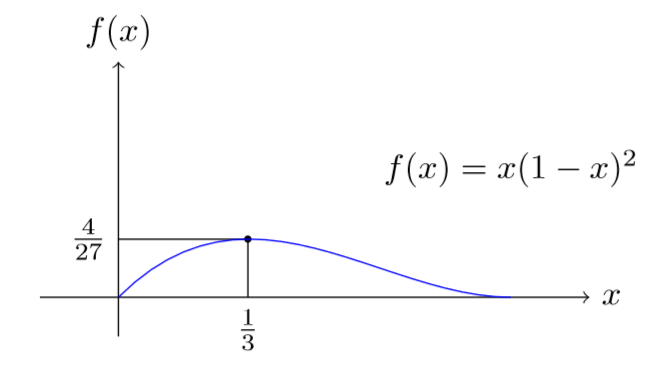
\includegraphics[width=0.45\linewidth]{Figures/figure2.1} 

}

\caption{Verosimilitud para $(0,1,0)$ de una muestra de $3$ de una Bernoulli}\label{fig:berlik}
\end{figure}

\hypertarget{S:frequency-distributions-mle}{%
\subsection{MLE de las distribuciones de frecuencias}\label{S:frequency-distributions-mle}}

A continuación derivamos el estimador de máxima verosimilitud, \emph{MLE}, para los tres miembros de la clase \((a,b,0)\). Empezamos resumiendo la discusión anterior. En el escenario de observar las variables aleatorias \emph{iid}, independientes e idénticamente distribuidas, \(X_1,X_2,\ldots,X_n\) de una distribución con \emph{pmf} \(p_\theta\), donde \(\theta\) toma un valor desconocido en \(\Theta\subseteq \mathbb{R}^d\), la verosimilitud \(L(\cdot)\), una función en \(\Theta\) se define como

\[
L(\theta):=\prod_{i=1}^n p_\theta(x_i),
\]
donde \(x_1,\ldots,x_n\) son los valores observados. El \emph{MLE} de \(\theta\), denotado como \(\hat{\theta}_{\rm MLE}\), es una función que asigna las observaciones a un elemento del conjunto de maximizadores de \(L(\cdot)\), concretamente
\[
\{\theta \vert L(\theta)=\max_{\eta\in\Theta}L(\eta)\}.
\]
Nótese que el conjunto anterior es una función de las observaciones, aunque esta dependencia no se muestra explícitamente.
En el caso de las tres distribuciones que estudiaremos, y de forma bastante general, el conjunto anterior es un conjunto unitario (singleton) con una probabilidad que tiende a uno (con un tamaño de muestra creciente). En otras palabras, para muchas distribuciones de uso común y cuando el tamaño de la muestra es grande, el estimador verosímil se define de forma única con una alta probabilidad.
A continuación, asumiremos que hemos observado \(n\) variables aleatorias \emph{iid} \(X_1,X_2,\ldots,X_n\) de la distribución considerada, aunque el valor del parámetro es desconocido. Además, \(x_1,x_2,\ldots,x_n\) denotará los valores observados. Cabe señalar en el caso de los datos de recuento, y de los datos de distribuciones discretas en general, que la verosimilitud puede representarse alternativamente como

\[
L(\theta):=\prod_{k\geq 0} \left(p_\theta(k)\right)^{m_k},
\]
donde
\[
m_k:= \left\vert \{i\vert x_i=k, 1\leq i \leq n\} \right\vert=\sum_{i= 1}^n I(x_i=k), \quad k\geq 0.
\]
Obsérvese que esta transformación conserva todos los datos, compilándolos de manera racionalizada. Para un \(n\) grande, lleva a la compresión de los datos en el sentido de \emph{suficiencia}. A continuación, presentamos las expresiones para el \emph{MLE} también en términos de \(\{m_k\}_{k\geq 1}\).

\textbf{MLE -- Distribución de Poisson:} En este caso, como se ha señalado anteriormente, la verosimilitud viene dada por
\[
L(\lambda)=\left(\prod_{i=1}^n x_i!\right)^{-1}e^{-n\lambda}\lambda^{\sum_{i=1}^n x_i},
\]
que implica
\[
l(\lambda)= -\sum_{i=1}^n \log(x_i!) -n\lambda +\log(\lambda) \cdot \sum_{i=1}^n x_i,
\]
y
\[
l'(\lambda)= -n +\frac{1}{\lambda}\sum_{i=1}^n x_i.
\]

En la evaluación de \(l''(\lambda)\), cuando \(\sum_{i=1}^n x_i>0\), \(l''< 0\). Por consiguiente, el máximo se alcanza en la media de la muestra, \(\overline{x}\), que se presenta a continuación. Cuando \(\sum_{i=1}^n x_i=0\), la verosimilitud es una función decreciente y, por lo tanto, el máximo se alcanza en el menor valor posible del parámetro; esto da como resultado que el estimador máximo verosímil sea cero. Por lo tanto, tenemos

\[
\overline{x} = \hat{\lambda}_{\rm MLE} = \frac{1}{n}\sum_{i=1}^n x_i. 
\]
Nótese que la media muestral puede calcularse también como
\[
\frac{1}{n} \sum_{k\geq 1} km_k.
\]

Cabe mencionar que en el caso de la Poisson, la distribución exacta de \(\hat{\lambda}_{\rm MLE}\) está disponible en forma cerrada - es una Poisson a escala - cuando la distribución subyacente es una Poisson. Esto es así porque la suma de variables aleatorias independientes de Poisson es también una Poisson. Por supuesto, para muestras de gran tamaño se puede utilizar el Teorema Central del Límite (CLT, según sus siglas en inglés) ordinario para derivar una aproximación normal. Nótese que esta última aproximación es válida si la distribución subyacente es una distribución con un segundo momento finito.

\textbf{MLE -- Distribución Binomial:} A diferencia del caso de la distribución de Poisson, el espacio de parámetros en el caso de la binomial es bidimensional. Por lo tanto, el problema de optimización es un poco más difícil. Podemos comenzar observando que la verosimilitud viene dada por

\[
L(m,q)= \left(\prod_{i=1}^n \binom{m}{x_i}\right) q^{\sum_{i=1}^n x_i} (1-q)^{nm-\sum_{i=1}^n x_i}, 
\]
y el logaritmo de la verosimilitud por
\[
l(m,q)= \sum_{i=1}^n \log\left(\binom{m}{x_i}\right) + \left({\sum_{i=1}^n x_i}\right)\log(q)+ \left({nm-\sum_{i=1}^n x_i}\right)\log(1-q). 
\]
Nótese que como \(m\) sólo toma valores enteros no negativos, no podemos usar cálculo multivariante para encontrar los valores óptimos. Sin embargo, podemos usar el cálculo para una sola variable para mostrar que
\begin{equation}
\hat{q}_{\rm MLE}\times \hat{m}_{\rm MLE}= \frac{1}{n}\sum_{i=1}^n X_i.  
\label{eq:binmle}
\end{equation}
En este sentido, observamos que para un valor fijado de \(m\),
\[
\frac{\delta}{\delta q} l(m,q) = \left({\sum_{i=1}^n x_i}\right)\frac{1}{q}- \left({nm-\sum_{i=1}^n x_i}\right)\frac{1}{1-q},
\]
y que
\[
\frac{\delta^2}{\delta q^2} l(m,q) = -\left[\left({\sum_{i=1}^n x_i}\right)\frac{1}{q^2} + \left({nm-\sum_{i=1}^n x_i}\right)\frac{1}{(1-q)^2}\right]\leq 0.
\]
Lo anterior implica que para un valor concreto de \(m\), el valor máximo de \(q\) satisface
\[
mq=\frac{1}{n}\sum_{i=1}^n X_i,
\]
y por lo tanto establecemos la ecuación \eqref{eq:binmle}. Lo anterior reduce la tarea a la búsqueda de \(\hat{m}_{\rm MLE}\), que es miembro del conjunto de los maximizadores de
\begin{equation}
L\left(m,\frac{1}{nm}\sum_{i=1}^n x_i\right).
\label{eq:binlikm}
\end{equation}
Nótese que la verosimilitud sería cero para valores de \(m\) menores a \(\max\limits_{1\leq i \leq n}x_i\), y por tanto
\[
\hat{m}_{\rm MLE}\geq \max_{1\leq i \leq n}x_i.
\]
Para especificar un algoritmo para calcular \(\hat{m}_{\rm MLE}\), primero señalamos que para algunos conjuntos de datos \(\hat{m}_{\rm MLE}\) podría ser igual a \(\infty\), lo que indicaría que una distribución de Poisson se ajustaría mejor que una distribución binomial. Esto es así, ya que la distribución binomial con los parámetros \((m,\overline{x}/m)\) se aproxima a la distribución de Poisson con el parámetro \(\overline{x}\) con \(m\) tendiendo a infinito. El hecho de que algunos conjuntos de datos \textbf{prefieran} una distribución de Poisson no debería ser sorprendente ya que desde este punto de vista el conjunto de la distribución de Poisson está en el límite del conjunto de las distribuciones binomiales.

Curiosamente, en \citep{olkin1981} muestran que si la media de la muestra es menor o igual a la varianza de la muestra entonces \(\hat{m}_{\rm MLE}=\infty\); de lo contrario, existe un \(m\) finito que maximiza la ecuación \eqref{eq:binlikm}. En la siguiente Figura \ref{fig:MLEm} se muestra el gráfico de \(L\left(m,\frac{1}{nm}\sum_{i=1}^n x_i\right)\) para tres muestras diferentes de tamaño \(5\); sólo difieren en el valor del máximo de la muestra. La primera muestra de \((2,2,2,4,5)\) tiene una relación entre la media de la muestra y la varianza de la muestra mayor a \(1\) (\(1,875\)), la segunda muestra de \((2,2,2,4,6)\) tiene la relación igual a \(1,25\) que está más cerca de \(1\), y la tercera muestra de \((2,2,2,4,7)\) tiene una relación menor a \(1\) (\(0,885\)). Para las tres muestras, como se muestra en la Figura \ref{fig:MLEm}, \(\hat{m}_{\rm MLE}\) es igual a \(7\), \(18\) and \(\infty\), respectivamente. Nótese que el valor en el límite de \(L\left(m,\frac{1}{nm}\sum_{i=1}^n x_i\right)\) cuando \(m\) tiende a infinito es igual a

\begin{equation}
\left(\prod_{i=1}^n x_i! \right)^{-1} \exp\left\{-\sum_{i=1}^n x_i\right\} \overline{x}^{n\overline{x}}. 
\label{eq:Poilik}
\end{equation}
También, se debe señalar que la Figura \ref{fig:MLEm} muestra que el \emph{MLE} de \(m\) es no robusto, \emph{i.e.}, pequeños cambios en el conjunto de datos pueden causar grandes cambios en el estimador.

La discusión anterior sugiere el siguiente algoritmo sencillo:

\begin{itemize}
\item
  \emph{Paso 1}. Si la media de la muestra es menor o igual a la varianza de la muestra, \(\hat{m}_{MLE}=\infty\). La distribución sugerida por \emph{MLE} es una distribución de Poisson con \(\hat{\lambda}=\overline{x}\).
\item
  \emph{Paso 2}. Si la media de la muestra es mayor que la varianza de la muestra, entonces calcula \(L(m,\overline{x}/m)\) para valores de \(m\) mayores o iguales al máximo de la muestra hasta que \(L(m,\overline{x}/m)\) se acerque al valor de la verosimilitud de Poisson dada en \eqref{eq:Poilik}. El valor de \(m\) que corresponde al valor máximo de \(L(m,\overline{x}/m)\) entre los calculados es igual a \(\hat{m}_{MLE}\).
\end{itemize}

Obsérvese que si la distribución subyacente es la distribución binomial con parámetros \((m,q)\) (con \(q>0\)) entonces \(\hat{m}_{MLE}\) será igual a \(m\) para los tamaños de muestra grandes. Además, \(\hat{q}_{MLE}\) tendrá una distribución asintóticamente normal y convergerá con probabilidad uno a \(q\).

\begin{figure}

{\centering 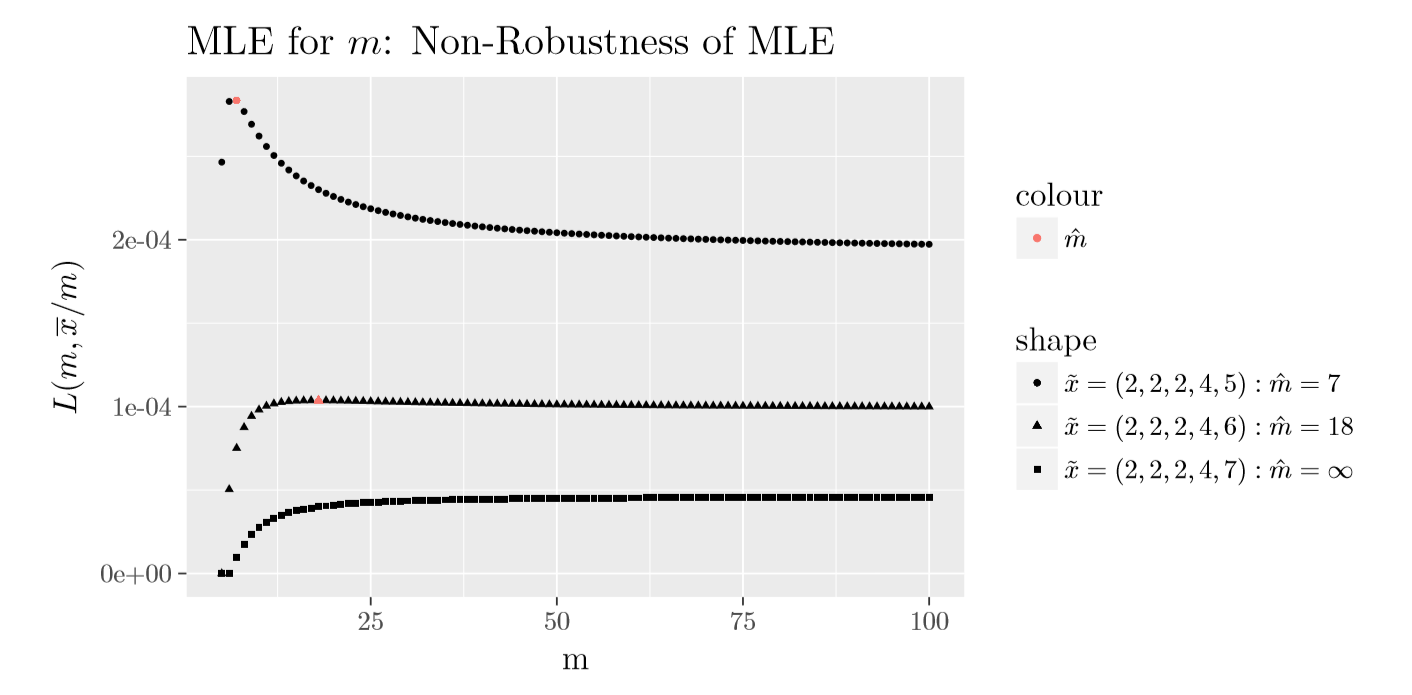
\includegraphics[width=0.8\linewidth]{Figures/figure2.2} 

}

\caption{Gráfico de $L(m,\overline{x}/m)$ de la distribución binomial}\label{fig:MLEm}
\end{figure}

\textbf{MLE -- Distribución Binomial Negativa:} El caso de la distribución binomial negativa es similar al de la distribución binomial en el sentido de que tenemos dos parámetros y los \emph{MLE} no existen en una forma cerrada. Una diferencia entre ellas es que, a diferencia del parámetro de la binomial \(m\) que toma valores enteros positivos, el parámetro \(r\) de la binomial negativa puede tomar cualquier valor real positivo. Esto hace que el problema de optimización sea un poco más complejo. Comencemos señalando que la verosimilitud puede expresarse de la siguiente forma:

\[
L(r,\beta)=\left(\prod_{i=1}^n \binom{r+x_i-1}{x_i}\right) (1+\beta)^{-n(r+\overline{x})} \beta^{n\overline{x}}.  
\]
Lo anterior implica que la log-verosimilitud viene dada por
\[
l(r,\beta)=\sum_{i=1}^n \log\binom{r+x_i-1}{x_i} -n(r+\overline{x}) \log(1+\beta) +n\overline{x}\log\beta,
\]
Y por tanto
\[
\frac{\delta}{\delta\beta} l(r,\beta) = -\frac{n(r+\overline{x})}{1+\beta} + \frac{n\overline{x}}{\beta}.
\]
Igualando la ecuación a cero, tenemos
\[
\hat{r}_{MLE}\times \hat{\beta}_{MLE} = \overline{x}.
\]
Lo anterior reduce el problema de optimización bidimensional a un problema unidimensional- se necesita maximizar
\[
l(r,\overline{x}/r)=\sum_{i=1}^n \log\binom{r+x_i-1}{x_i} -n(r+\overline{x}) \log(1+\overline{x}/r) +n\overline{x}\log(\overline{x}/r),
\]
con respecto a \(r\), siendo el maximizador de \(r\) su \emph{MLE} y \(\hat{\beta}_{MLE}=\overline{x}/\hat{r}_{MLE}\). En \citep{levin1977} se muestra que si la varianza muestral es mayor que la media muestral, entonces existe un único \(r>0\) que maximiza \(l(r,\overline{x}/r)\) y por lo tanto un único \emph{MLE} para \(r\) y \(\beta\). Además, muestran que si \(\hat{\sigma}^2\leq \overline{x}\), entonces la verosimilitud de la binomial negativa estará dominada por la verosimilitud de la Poisson con \(\hat{\lambda}=\overline{x}\). En otras palabras, una distribución de Poisson ofrece un mejor ajuste a los datos. La garantía en el caso de \(\hat{\sigma}^2>\hat{\mu}\) nos permite usar un algoritmo para maximizar \(l(r,\overline{x}/r)\). Mediante un método alternativo de calcular la verosimilitud, observamos que
\[
l(r,\overline{x}/r)=\sum_{i=1}^n \sum_{j=1}^{x_i}\log(r-1+j) - \sum_{i=1}^n\log(x_i!) - n(r+\overline{x}) \log(r+\overline{x}) + nr\log(r) + n\overline{x}\log(\overline{x}),
\]
lo que genera
\[
\left(\frac{1}{n}\right)\frac{\delta}{\delta r}l(r,\overline{x}/r)=\left(\frac{1}{n}\right)\sum_{i=1}^n \sum_{j=1}^{x_i}\frac{1}{r-1+j} - \log(r+\overline{x}) + \log(r).
\]
Observamos que, en las expresiones anteriores para los términos que implican un doble sumatorio, el sumatorio interno es igual a cero si \(x_i=0\). El \emph{estimador máximo verosímil} de \(r\) es una raíz de la última expresión y podemos usar un algoritmo de búsqueda de raíces para calcularla. Además, tenemos

\[
\left(\frac{1}{n}\right)\frac{\delta^2}{\delta r^2}l(r,\overline{x}/r)=\frac{\overline{x}}{r(r+\overline{x})}-\left(\frac{1}{n}\right)\sum_{i=1}^n \sum_{j=1}^{x_i}\frac{1}{(r-1+j)^2}.
\]
Un algoritmo iterativo de búsqueda de raíces simple y de rápida convergencia es el método de Newton, que se cree que los Babilonios ya utilizaban para calcular raíces cuadradas. Con este método, se selecciona una aproximación inicial para la raíz y se generan sucesivamente nuevas aproximaciones para la raíz hasta la convergencia. Aplicando el método de Newton a nuestro problema se obtiene el siguiente algoritmo:\\
\emph{Paso i}. Elegir una solución aproximada, denominada \(r_0\). Fijar \(k\) igual a \(0\).\\
\emph{Paso ii}. Definir \(r_{k+1}\) como
\[
r_{k+1}:= r_k - \frac{\left(\frac{1}{n}\right)\sum_{i=1}^n \sum_{j=1}^{x_i}\frac{1}{r_k-1+j} - \log(r_k+\overline{x}) + \log(r_k)}{\frac{\overline{x}}{r_k(r_k+\overline{x})}-\left(\frac{1}{n}\right)\sum_{i=1}^n \sum_{j=1}^{x_i}\frac{1}{(r_k-1+j)^2}}
\]\\
\emph{Paso iii}. Si \(r_{k+1}\sim r_k\), entonces establece \(r_{k+1}\) como \emph{estimador máximo verosímil}; en otro caso, incrementa \(k\) por \(1\) y repite \emph{Paso ii}.

Por ejemplo, simulamos una muestra de \(5\) observaciones de \(41, 49, 40, 27, 23\) de la binomial negativa con los parámetros \(r=10\) y \(\beta=5\). Escogiendo el valor inicial de \(r\) de tal manera que
\[
r\beta=\hat{\mu} \quad \hbox{and} \quad r\beta(1+\beta)=\hat{\sigma}^2
\]
donde \(\hat{\mu}\) representa la media estimada y \(\hat{\sigma}^2\) es la varianza estimada. Esto nos conduce a un valor inicial de \(r\) de \(23,14286\). Las iteraciones de \(r\) del método de Newton son
\[
21,39627, 21,60287, 21,60647, 21,60647;
\]
la rápida convergencia anterior es frecuente con el método de Newton. Por lo tanto, en este ejemplo, \(\hat{r}_{MLE}\sim21,60647\) y \(\hat{\beta}_{MLE}=8,3308\).

\emph{Implementación R del Método de Newton - MLE binomial negativa para \(r\)}

\begin{verbatim}
Newton<-function(x,abserr){
mu<-mean(x);
sigma2<-mean(x^2)-mu^2;
r<-mu^2/(sigma2-mu);
b<-TRUE;
iter<-0;
while (b) {
tr<-r;
m1<-mean(c(x[x==0],sapply(x[x>0],function(z){sum(1/(tr:(tr-1+z)))})));
m2<-mean(c(x[x==0],sapply(x[x>0],function(z){sum(1/(tr:(tr-1+z))^2)})));
r<-tr-(m1-log(1+mu/tr))/(mu/(tr*(tr+mu))-m2);
b<-!(abs(tr-r)<abserr);
iter<-iter+1;
}
c(r,iter)
}
\end{verbatim}

\begin{center}\rule{0.5\linewidth}{0.5pt}\end{center}

Para concluir nuestra discusión sobre \emph{MLE} para la clase de distribuciones \((a,b,0)\), en la Figura \ref{fig:MLEab0} siguiente representamos gráficamente el valor máximo de la verosimilitud de Poisson, \(L(m,\overline{x}/m)\) para la binomial, y \(L(r,\overline{x}/r)\) para la binomial negativa, para las tres muestras de tamaño \(5\) dadas en \protect\hyperlink{tab:2.1}{Tabla 2.1}. Los datos se construyeron de tal forma que cubrieran las tres ordenaciones entre la media y varianza muestrales.
Como se muestra en la Figura \ref{fig:MLEab0}, y demostrado por la teoría, si \(\hat{\mu}<\hat{\sigma}^2\)
entonces la binomial negativa dará un mayor valor del máximo de verosimilitud; si \(\hat{\mu}=\hat{\sigma}^2\) la Poisson dará el mayor valor de la verosimilitud; y finalmente en el caso que \(\hat{\mu}>\hat{\sigma}^2\) la binomial dará un mejor ajuste que las otras. Así que, antes de ajustar los datos con una distribución de frecuencias \((a,b,0)\), es mejor empezar por examinar el orden entre \(\hat{\mu}\) y \(\hat{\sigma}^2\). Cabe volver a enfatizar que la Poisson está en el \textbf{límite} de las distribuciones binomial negativa y binomial. Por lo tanto en el caso que \(\hat{\mu}\geq\hat{\sigma}^2\) (\(\hat{\mu}\leq\hat{\sigma}^2\), resp.) la Poisson dará un mejor ajuste que la binomial negativa (binomial, resp.), que también se indicará con \(\hat{r}=\infty\) (\(\hat{m}=\infty\), resp.).

\[\begin{matrix}
\begin{array}{c|c|c}
\hline
\text{Datos} & \text{Media }(\hat{\mu}) & \text{Varianza }(\hat{\sigma}^2) \\
\hline
(2,3,6,8,9) & 5,60 & 7,44 \\ 
(2,5,6,8,9) & 6 & 6\\
(4,7,8,10,11) & 8 & 6\\\hline
\end{array}
\end{matrix}\]

\protect\hyperlink{tab:2.1}{Tabla 2.1} : Tres Muestras de Tamaño \(5\)

\begin{figure}

{\centering 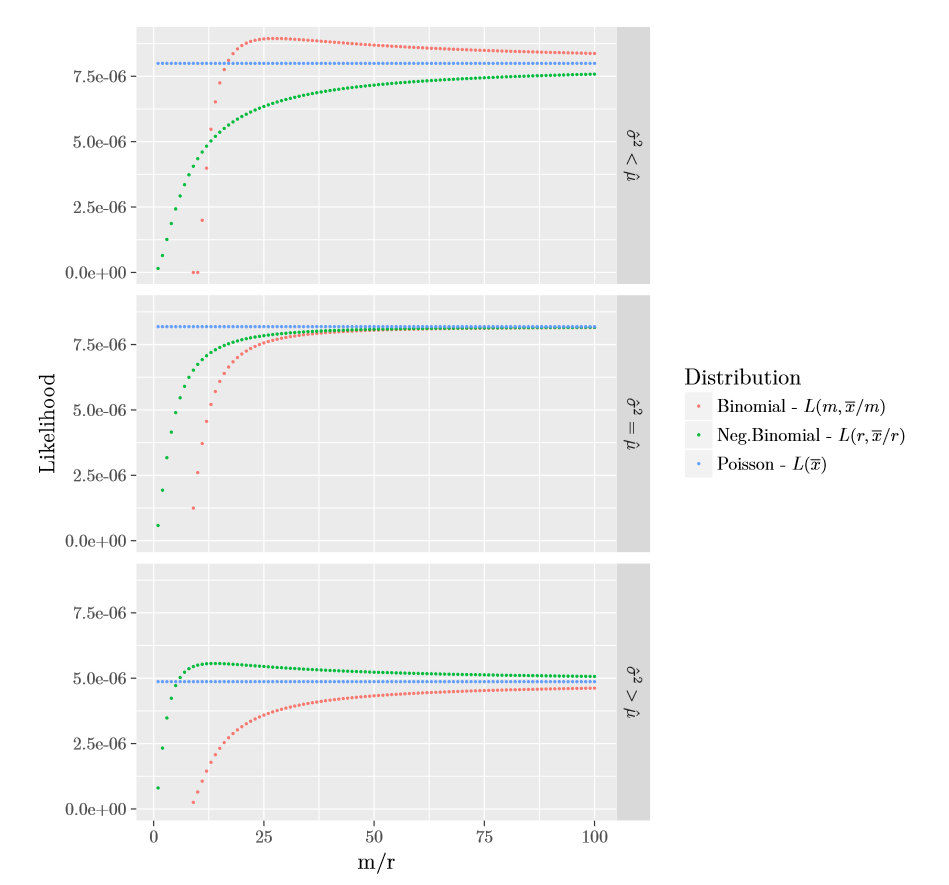
\includegraphics[width=0.8\linewidth]{Figures/figure2.3} 

}

\caption{Gráfico de las Verosimilitudes Parcialmente Maximizadas $(a,b,0)$}\label{fig:MLEab0}
\end{figure}

\hypertarget{S:other-frequency-distributions}{%
\section{Otras Distribuciones de Frecuencias}\label{S:other-frequency-distributions}}

\begin{center}\rule{0.5\linewidth}{0.5pt}\end{center}

En esta sección, se aprende a:

\begin{itemize}
\tightlist
\item
  Definir la clase de distribuciones de frecuencia (a,b,1) y discutir la importancia de la relación recursiva que sustenta esta clase de distribuciones
\item
  Interpretar las versiones truncadas y modificadas en cero de las distribuciones binomiales, Poisson y binomial negativa
\item
  Calcular las probabilidades usando la relación recursiva
\end{itemize}

\begin{center}\rule{0.5\linewidth}{0.5pt}\end{center}

En las secciones anteriores hemos examinado tres distribuciones con soporte definido en el conjunto de números enteros no negativos, que se adaptan bien a muchas aplicaciones de seguros. Además, al permitir frecuentemente que los parámetros sean una función de variables explicativas conocidas (por el asegurador) como la edad, el sexo, la ubicación geográfica (territorio), etc., estas distribuciones nos permiten explicar las probabilidades de siniestro en términos de estas variables. El ámbito de la estadística que analiza estos modelos se conoce como análisis de regresión - es un tópico importante de interés actuarial que no se tratará en este libro; ver \citep{freesregression}.

Es evidente que existen infinitas otras distribuciones de recuento, y lo que es más importante, las distribuciones anteriores por sí mismas no satisfacen todas las necesidades prácticas. En concreto, una característica de algunos datos en seguros es que la proporción de ceros puede ser muy diferente en la relación a la proporción de otros valores para que puedan ser explicados por las distribuciones anteriores. A continuación, se modifican las distribuciones previas para permitir una probabilidad arbitraria para el recuento de ceros, independientemente de la asignación relativa de probabilidades para los otros valores. Otra característica de un conjunto de datos que está compuesto por subconjuntos homogéneos es que, aunque las distribuciones anteriores pueden proporcionar buenos ajustes a cada subconjunto, pueden no hacerlo para la totalidad del conjunto de datos. Posteriormente, se amplían de forma natural las distribuciones \((a,b,0)\) para poder cubrir, en particular, estos conjuntos de datos.

\hypertarget{S:zero-truncation-or-modification}{%
\subsection{Modificación o Truncamiento en Cero}\label{S:zero-truncation-or-modification}}

Supongamos que analizamos pólizas del seguro de automóvil que aparecen en una base de datos de siniestros de automóvil ocurridos en un determinado período. Si se estudia el número de siniestros que estas pólizas han tenido durante este período, entonces obviamente la distribución tiene que asignar una probabilidad de cero a la variable de recuento que asume el valor cero. En otras palabras, al restringir la atención a los datos de recuento en las pólizas de la base de datos de siniestros, en cierto modo hemos truncado en cero los datos de recuento de todas las pólizas. En productos de seguros a particulares (como en el caso de los automóviles), los asegurados pueden no querer informar del primer siniestro por temor a que aumente el precio del seguro en el futuro - este comportamiento inflará la proporción de recuentos de cero. Ejemplos como estos últimos modifican la proporción de ceros. Es interesante mencionar que las modificaciones naturales de las tres distribuciones anteriores son capaces de proporcionar buenos ajustes a los conjuntos de datos cero modificados/truncados que se generan en el seguro.

Como se presenta a continuación, se modifica la probabilidad que se le asigna al valor cero en la clase \((a,b,0)\) manteniendo las probabilidades relativas asignadas a los valores no nulos - modificación en cero. Nótese que como la clase de distribuciones \((a,b,0)\) satisface la recurrencia \eqref{eq:ab0}, el mantenimiento de las probabilidades relativas de los valores no nulos implica que la recurrencia \eqref{eq:ab0} se satisface para \(k\geq 2\). Esto nos lleva a la definición de la siguiente clase de distribuciones.

\textbf{Definición}. Una distribución de recuento es un miembro de la clase \((a, b, 1)\) si para las constantes \(a\) y \(b\) las probabilidades \(p_k\) satisfacen
\begin{equation}
\frac{p_k}{p_{k-1}}=a+\frac{b}{k},\quad k\geq 2.
\label{eq:ab1}
\end{equation}

Nótese que como la recursión empieza en \(p_1\), y no en \(p_0\), nos referimos a esta superclase de distribuciones \((a,b,0)\) como (a,b,1). Para entender esta clase, recordemos que cada par de valores válidos para \(a\) y \(b\) de la clase \((a,b,0)\) corresponde a un único vector de probabilidades \(\{p_k\}_{k\geq 0}\). Si ahora observamos el vector de probabilidades \(\{\tilde{p}_k\}_{k\geq 0}\) dado por

\[
\tilde{p}_k= \frac{1-\tilde{p}_0}{1-p_0}\cdot p_k, \quad k\geq 1,
\]

donde \(\tilde{p}_0\in[0,1)\) se elige arbitrariamente, entonces como las probabilidades relativas de valores positivos de acuerdo con \(\{p_k\}_{k\geq 0}\) y \(\{\tilde{p}_k\}_{k\geq 0}\) son las mismas, tenemos que \(\{\tilde{p}_k\}_{k\geq 0}\) satisface la recurrencia \eqref{eq:ab1}. Esto, en particular, muestra que la clase de distribuciones \((a,b,1)\) es estrictamente más amplia que la \((a,b,0)\).

Previamente, hemos establecido un par de valores para \(a\) y \(b\) que llevaron a una distribución válida de \((a,b,0)\), y luego miramos las distribuciones \((a,b,1)\) que correspondían a esta distribución \((a,b,0)\). Ahora argumentaremos que la clase \((a,b,1)\) admite un conjunto mayor de distribuciones permitidas para \(a\) y \(b\) que la clase \((a,b,0)\). Recordemos de la Sección \ref{S:the-a-b-0-class} que en el caso de \(a<0\) no se utiliza el hecho de que la recurrencia \eqref{eq:ab0} empieza en \(k=1\), y por lo tanto el conjunto de pares \((a,b)\) con \(a<0\) que son admisibles para la clase \((a,b,0)\) es idéntico al que es admisible para la clase \((a,b,1)\). La misma conclusión se puede extraer fácilmente para los pares con \(a=0\). En el caso que \(a>0\), en lugar de la restricción \(a+b>0\) para la clase \((a,b,0)\), tenemos ahora la restricción más débil de \(a+b/2>0\) para la clase \((a,b,1)\). Con la parametrización \(b=(r-1)a\) utilizada en la Sección \ref{S:the-a-b-0-class}, en lugar de \(r>0\) tenemos ahora la restricción más débil de \(r>-1\). En particular, vemos que mientras que al modificar el cero en una distribución \((a,b,0)\) conduce a una distribución de la clase \((a,b,1)\), está conclusión no se cumple en la dirección contraria.

La modificación en cero de una distribución de recuento \(F\) tal que asigna una probabilidad cero al valor cero se llama un truncamiento en cero de \(F\). De este modo, la versión truncada en cero de las probabilidades \(\{p_k\}_{k\geq 0}\) viene dada por

\[
\tilde{p}_k=\begin{cases}
0, & k=0;\\
\frac{p_k}{1-p_0}, & k\geq 1.
\end{cases}
\]

En concreto, tenemos que una modificación en cero de una distribución de recuento \(\{p_k^T\}_{k\geq 0}\), denotada por \(\{p^M_k\}_{k\geq 0}\), puede escribirse como una combinación convexa de la distribución degenerada en \(0\) y el truncamiento en cero de \(\{p_k\}_{k\geq 0}\), denotado por \(\{p^T_k\}_{k\geq 0}\). De este modo tenemos

\[
p^M_k= p^M_0 \cdot \delta_{0}(k) + (1-p^M_0) \cdot p^T_k, \quad k\geq 0.  
\]

\textbf{Ejemplo 2.5.1. Poisson Cero Modificada/Truncada}.
Considerar una distribución de Poisson con parámetro \(\lambda=2\). Calcular \(p_k, k=0,1,2,3\), para la usual (sin modificar), truncada y una versión modificada con \((p_0^M=0,6)\).

\textbf{Solución.} Para la distribución de Poisson como miembro de la clase ((\(a,b\),0), tenemos \(a=0\) y \(b=\lambda=2\). Por lo tanto, podemos usar para cada tipo la recursión \(p_k = \lambda p_{k-1}/k= 2 p_{k-1}/k\), después de determinar las probabilidades iniciales. El cálculo de probabilidades para \(k\leq 3\) se muestra en \protect\hyperlink{tab:2.2}{Tabla 2.2}.

\[\begin{matrix}
\begin{array}{c|c|c|c}
\hline
k & p_k & p_k^T & p_k^M\\\hline
0 & p_0=e^{-\lambda}=0,135335 & 0 & 0,6\\\hline
1 & p_1=p_0(0+\frac{\lambda}{1})=0,27067 &
\frac{p_1}{1-p_0}=0,313035 &
\frac{1-p_0^M}{1-p_0}~p_1=0,125214\\\hline
2 & p_2=p_1\left( \frac{\lambda}{2}\right)=0,27067 &
p_2^T=p_1^T\left(\frac{\lambda}{2}\right)=0,313035 &
p_2^M=p_1^M\left(\frac{\lambda}{2}\right)=0,125214\\\hline
3 & p_3=p_2\left(\frac{\lambda}{3}\right)=0,180447 &
p_3^T=p_2^T\left(\frac{\lambda}{3}\right)=0,208690 &
p_3^M=p_2^M\left(\frac{\lambda}{3}\right)=0,083476\\\hline
\end{array}
\end{matrix}\]

\protect\hyperlink{tab:2.2}{Tabla 2.2} : Cálculo de probabilidades para \(k\leq 3\)

\begin{center}\rule{0.5\linewidth}{0.5pt}\end{center}

\hypertarget{S:mixture-distributions}{%
\section{Distribuciones Mixtas}\label{S:mixture-distributions}}

\begin{center}\rule{0.5\linewidth}{0.5pt}\end{center}

En esta sección, se aprende a:

\begin{itemize}
\tightlist
\item
  Definir una distribución mixta cuando el componente de mixtura se basa en un número finito de subgrupos
\item
  Calcular las probabilidades de la distribución mixta a partir de las proporciones de la mixtura y el conocimiento de la distribución de cada subgrupo
\item
  Definir una distribución mixta cuando el componente de mixtura es continuo
\end{itemize}

\begin{center}\rule{0.5\linewidth}{0.5pt}\end{center}

En muchas aplicaciones la población subyacente consiste en subgrupos definidos de forma natural con cierta homogeneidad dentro de cada subgrupo. En estos casos es conveniente modelizar los subgrupos individuales y, de manera fundamentada, modelizar el conjunto de la población. Como veremos más adelante, más allá del atractivo del enfoque, también se amplía el abanico de aplicaciones que pueden cubrirse mediante las distribuciones paramétricas estándar.

Supongamos que \(k\) denota el número de subgrupos definidos en una población, y \(F_i\) denota la distribución de una observación extraída del subgrupo \(i\)-ésimo. Si dejamos que \(\alpha_i\) denote la proporción de la población en el subgrupo \(i\)-ésimo, con \(\sum_{i=1}^k \alpha_i=1\), entonces la distribución de una observación elegida al azar de la población, denotada por \(F\), viene dada por

\begin{equation}
F(x)=\sum_{i=1}^k \alpha_i \cdot F_i(x).
\label{eq:mixdefn}
\end{equation}

La expresión anterior puede considerarse una aplicación directa de la Ley de Probabilidad Total. Como ejemplo, consideremos una población de conductores dividida en dos subgrupos, los que tienen como máximo \(5\) años de experiencia de conducción y los que tienen más de \(5\) años de experiencia. Supongamos que \(\alpha\) denota la proporción de conductores con menos de \(5\) años de experiencia, y \(F_{\leq 5}\) y \(F_{> 5}\) denotan la distribución del número de siniestros en un año para un conductor de cada grupo, respectivamente. Entonces la distribución del número de siniestros de un conductor seleccionado al azar viene dada por

\[
\alpha\cdot F_{\leq 5}(x) + (1-\alpha)F_{> 5}(x).
\]

Una definición alternativa de una distribución mixta es la siguiente. Supongamos que \(N_i\) es una variable aleatoria con distribución \(F_i\), \(i=1,\ldots, k\). Sea \(I\) una variable aleatoria que toma valores \(1,2,\ldots,k\) con probabilidades \(\alpha_1,\ldots,\alpha_k\), respectivamente. Entonces, la variable aleatoria \(N_I\) tiene una distribución dada por la ecuación \eqref{eq:mixdefn}\footnote{Esto, en concreto, establece una forma de simular a partir de una distribución mixta que hace uso de los eficientes esquemas de simulación que pueden existir para las distribuciones que la componen.}.

En \eqref{eq:mixdefn} vemos que la función de distribución es una combinación convexa de las funciones de distribución que la componen. Este resultado se extiende fácilmente a la función de densidad, la función de supervivencia, los momentos ordinarios y el valor esperado, ya que todos ellos son aplicaciones lineales de la función de distribución. Observamos que esto no es cierto en el caso de los momentos centrales como la varianza, y de las medidas condicionales como la función de tasa de riesgo (hazard rate). En el caso de la varianza se ve fácilmente como

\begin{equation}
\mathrm{Var}{[N_I]}=\mathrm{E}[{\mathrm{Var}[{N_I\vert I}]]} + \mathrm{Var}[{\mathrm{E}[{N_I|I}}]]=\sum_{i=1}^k \alpha_i \mathrm{Var}[{N_i}] + \mathrm{Var}[{\mathrm{E}[{N_I|I}}]] .
\label{eq:LawTotalVariation}
\end{equation}

El Apéndice \ref{C:AppB} proporciona información adicional sobre esta importante expresión.

\textbf{Ejemplo 2.6.1. Pregunta de Examen Actuarial}.
En una determinada ciudad el número de resfriados comunes que un individuo tendrá en un año sigue una distribución de Poisson que depende de la edad del individuo y su condición de fumador. La distribución de la población y el número medio de resfriados son los siguientes:

\[\begin{matrix}
\begin{array}{l|c|c}
\hline
 & \text{Proporción de población} &
\text{Número medio de resfriados}\\\hline
\text{Niños} & 0,3 & 3\\
\text{Adultos No-fumadores} & 0,6 & 1\\
\text{Adultos Fumadores} & 0,1 & 4\\\hline
\end{array}
\end{matrix}\]

\protect\hyperlink{tab:2.3}{Tabla 2.3} : La distribución de la población y el número medio de resfriados

\begin{enumerate}
\def\labelenumi{\arabic{enumi}.}
\tightlist
\item
  Calcular la probabilidad de que una persona seleccionada al azar tenga 3 resfriados comunes en un año.
\item
  Calcular la probabilidad condicionada de que una persona con exactamente 3 resfriados comunes en un año sea un fumador adulto.
\end{enumerate}

\textbf{Solución.}

\begin{enumerate}
\def\labelenumi{\arabic{enumi}.}
\item
  Utilizando la Ley de Probabilidad Total, podemos escribir la probabilidad requerida como \(\Pr(N_I=3)\), con \(I\) que denota el grupo del individuo seleccionado al azar con \(1,2\) y \(3\) que significan los grupos \emph{Niños}, \emph{Adulto No Fumador}, y \emph{Adulto Fumador}, respectivamente. Ahora, por el condicionamiento, tenemos
  \[
  \Pr(N_I=3)=0,3\cdot\Pr(N_1=3)+0,6\cdot\Pr(N_2=3)+0,1\cdot\Pr(N_3=3),
  \]
  con \(N_1,N_2\) y \(N_3\) que siguen una distribución de Poisson de media \(3,1\), y \(4\), respectivamente. Utilizando lo anterior, obtenemos \(\Pr(N_I=3)\sim0,1235\)
\item
  La probabilidad condicionada del evento A dado el evento B, \(\Pr(A\vert B) = \frac{\Pr(A,B)}{\Pr(B)}\). La probabilidad condicionada requerida en este problema puede escribirse como \(\Pr(I=3\vert N_I=3)\), que es igual a
\end{enumerate}

\[
\Pr(I=3\vert N_I=3)=\frac{\Pr(I=3,N_3=3)}{\Pr(N_I=3)}\sim\frac{0,1 \times 0,1954}{0,1235}\sim 0,1581.
\]

\begin{center}\rule{0.5\linewidth}{0.5pt}\end{center}

En el ejemplo previo, el número de subgrupos \(k\) era igual a tres. En general, \(k\) puede ser cualquier número natural, pero cuando \(k\) es grande es parsimonioso desde el punto de vista de la modelización tomar el siguiente enfoque de \emph{infinitamente muchos subgrupos}. Para justificar este enfoque, supongamos que el subgrupo \(i\)-ésimo sea tal que su distribución componente \(F_i\) viene dada por \(G_{\tilde{\theta_i}}\), donde \(G_\cdot\) es una familia paramétrica de distribuciones con espacio paramétrico \(\Theta\subseteq \mathbb{R}^d\). Con este supuesto, la función de distribución \(F\) de una observación extraída aleatoriamente de la población viene dada por

\[
F(x)=\sum_{i=1}^k \alpha_i G_{\tilde{\theta_i}}(x),\quad \forall x\in\mathbb{R}.
\]
que puede escribirse alternativamente como
\[
F(x)=\mathrm{E}[{G_{\tilde{\vartheta}}(x)}],\quad \forall x\in\mathbb{R},
\]
donde \(\tilde{\vartheta}\) toma valores \(\tilde{\theta_i}\) con probabilidad \(\alpha_i\), para \(i=1,\ldots,k\). Esto muestra que cuando \(k\) es grande, se puede modelizar lo anterior tratando \(\tilde{\vartheta}\) como una variable aleatoria continua.

Para ilustrar este enfoque, supongamos que tenemos una población de conductores con la distribución de siniestros de un conductor individual que se distribuye como una Poisson. Cada persona tiene su propio (personal) número esperado de siniestros \(\lambda\) - valores más pequeños para los buenos conductores, y valores más grandes para el resto. Hay una distribución de \(\lambda\) en la población; una opción común y conveniente para la modelización de esta distribución es una distribución gamma con parámetros \((\alpha, \theta)\). Con estas características resulta que la distribución resultante de \(N\), los siniestros de un conductor elegido aleatoriamente, es una binomial negativa con parámetros \((r=\alpha,\beta=\theta)\). Esto puede mostrarse de muchas maneras, pero una forma sencilla es la siguiente:

\begin{align*}
\Pr(N=k)&= \int_0^\infty \frac{e^{-\lambda}\lambda^k}{k!} \frac{\lambda^{\alpha-1}e^{-\lambda/\theta}}{\Gamma{(\alpha)}\theta^{\alpha}} {\rm d}\lambda = 
\frac{1}{k!\Gamma(\alpha)\theta^\alpha}\int_0^\infty \lambda^{\alpha+k-1}e^{-\lambda(1+1/\theta)}{\rm d}\lambda=\frac{\Gamma{(\alpha+k)}}{k!\Gamma(\alpha)\theta^\alpha(1+1/\theta)^{\alpha+k}} \\
&=\binom{\alpha+k-1}{k}\left(\frac{1}{1+\theta}\right)^\alpha\left(\frac{\theta}{1+\theta}\right)^k, \quad k=0,1,\ldots
\end{align*}
Obsérvese que la derivación previa utiliza implícitamente lo siguiente:
\[
f_{N\vert\Lambda=\lambda}(N=k)=\frac{e^{-\lambda}\lambda^k}{k!}, \quad k\geq 0; \quad \hbox{y} \quad f_{\Lambda}(\lambda)= \frac{\lambda^{\alpha-1}e^{-\lambda/\theta}}{\Gamma{(\alpha)}\theta^{\alpha}}, \quad \lambda>0.
\]

Cabe mencionar que al considerar las mixturas de una clase paramétrica de distribuciones se incrementa la riqueza de la clase. Esta expansión de las distribuciones da como resultado que la clase de mixtura pueda adaptarse bien a más aplicaciones que la clase paramétrica inicial. La modelización de mixturas es una técnica de modelización muy importante en las aplicaciones de seguros, y en los capítulos posteriores se tratarán más aspectos de esta técnica de modelización.

\textbf{Ejemplo 2.6.2.}
Supongamos que \(N|\Lambda \sim\) Poisson\((\Lambda)\) y que \(\Lambda \sim\) gamma con media de 1 y varianza de 2. Determinar la probabilidad que \(N=1\).

\textbf{Solución.} Para una distribución gamma con parámetros \((\alpha, \theta)\), tenemos que la media es \(\alpha \theta\) y la varianza es \(\alpha \theta^2\). En base a estas expresiones tenemos que
\[
\begin{aligned}
\alpha &= \frac{1}{2} \text{   y   } \theta =2.
\end{aligned}
\]
Ahora, se puede utilizar directamente el resultado anterior para concluir que \(N\) se distribuye como una binomial negativa con \(r = \alpha = \frac{1}{2}\) y \(\beta= \theta =2\). Por lo tanto,
\[
\begin{aligned}
\Pr(N=1)  &= \binom{1+r-1}{1}(\frac{1}{(1+\beta)^r})\left(\frac{\beta}{1+\beta}\right)^1 \\
&=                 \binom{1+\frac{1}{2}-1}{1}{\frac{1}{(1+2)^{1/2}}}\left(\frac{2}{1+2}\right)^1\\
&=  \frac{1}{3^{3/2}} = 0,19245 .
\end{aligned}
\]

\begin{center}\rule{0.5\linewidth}{0.5pt}\end{center}

\hypertarget{S:goodness-of-fit}{%
\section{Bondad del Ajuste}\label{S:goodness-of-fit}}

\begin{center}\rule{0.5\linewidth}{0.5pt}\end{center}

En esta sección, se aprende a:

\begin{itemize}
\tightlist
\item
  Calcular un estadístico de bondad del ajuste para comparar una distribución discreta hipotética con una muestra de observaciones discretas
\item
  Comparar el estadístico con una distribución de referencia para evaluar la adecuación del ajuste
\end{itemize}

\begin{center}\rule{0.5\linewidth}{0.5pt}\end{center}

Previamente se han analizado tres distribuciones de frecuencias elementales, junto con sus extensiones mediante la modificación/truncamiento en cero y mostrando las mixturas de estas distribuciones. Ahora bien, estas clases siguen siendo paramétricas y, por tanto, por su propia naturaleza, un pequeño subconjunto de la clase de todas las distribuciones de frecuencia posibles (\emph{i.e.} el conjunto de distribuciones para números enteros no negativos.) Por lo tanto, aunque hemos mostrado métodos para estimar los parámetros desconocidos, la distribución \emph{ajustada} no será una buena representación de la distribución subyacente si ésta está \textbf{lejos} de la clase de distribución utilizada en la modelización. De hecho, se puede demostrar que el \emph{estimador máximo verosímil} convergerá a un valor de tal forma que la distribución correspondiente será una \emph{proyección} Kullback-Leibler de la distribución subyacente en la clase de distribuciones utilizada para la modelización. A continuación presentamos un método de contraste - el estadístico chi-cuadrado de Pearson - para comprobar la bondad del ajuste de la distribución ajustada. Para más detalles sobre el contraste chi-cuadrado de Pearson, a un nivel introductorio de estadística matemática, remitimos al lector a la Sección 9.1 de \citep{zimmerman2015}.

En \(1993\), una cartera de \(n=7.483\) pólizas de seguro de automóvil de una importante compañía de seguros de Singapur tenía la distribución de accidentes de automóvil por asegurado como se indica en \protect\hyperlink{tab:2.4}{Tabla 2.4}.

\[\begin{matrix}
\begin{array}{c|c|c|c|c|c|c}
\hline
\text{Número }(k) & 0 & 1 & 2 & 3 & 4 & \text{Total}\\
\hline
\text{No. de Pólizas con }k\text{ accidentes }(m_k) & 6.996 & 455 & 28 & 4 & 0 & 7483\\
\hline
\end{array}
\end{matrix}\]

\protect\hyperlink{tab:2.4}{Tabla 2.4} : Datos de Accidentes de Automóvil en Singapur

Si se ajusta una distribución de Poisson, entonces el \emph{MLE} para \(\lambda\), la media de la Poisson, es la media muestral que es igual a
\[
\overline{N} = \frac{0\cdot 6996 + 1 \cdot 455 + 2 \cdot 28 + 3 \cdot 4 + 4 \cdot 0}{7483} = 0,06989.
\]
Ahora si se usa la Poisson (\(\hat{\lambda}_{MLE}\)) como la distribución ajustada, entonces una comparación tabular de los valores ajustados y los valores observados se muestra en la \protect\hyperlink{tab:2.5}{Tabla 2.5} siguiente, donde \(\hat{p}_k\) representa las probabilidades estimadas mediante la distribución de Poisson ajustada.

\[\begin{matrix}
\begin{array}{c|c|c}
\hline
\text{Número}  & \text{Observado}  & \text{Ajustado}\\
(k) & (m_k) & \text{Usando Poisson }(n\hat{p}_k)\\
\hline
0 & 6.996 & 6.977,86 \\
1 & 455 & 487,70 \\
2 & 28 & 17,04 \\
3 & 4 & 0,40 \\
\geq4 & 0 & 0,01\\
\hline
\text{Total} & 7.483 & 7.483,00\\
\hline
\end{array}
\end{matrix}\]

\protect\hyperlink{tab:2.5}{Tabla 2.5} : Comparación entre valores observados y ajustados: Datos de automóviles de Singapur

Mientras que el ajuste parece \emph{razonable}, una comparación tabular no es suficiente como contraste estadístico de la hipótesis de que la distribución subyacente es efectivamente la Poisson. El estadístico de chi-cuadrado de Pearson es una medida de bondad del ajuste que puede utilizarse para este propósito. Para explicar este estadístico, supongamos que un conjunto de datos de tamaño \(n\) se agrupa en \(k\) celdas, siendo \(m_k/n\) y \(\hat{p}_k\), para \(k=1\ldots,K\), las probabilidades observadas y estimadas de que una observación pertenezca a la celda \(k\)-ésima, respectivamente. El estadístico del contraste chi-cuadrado de Pearson viene dado por

\[
\sum_{k=1}^K\frac{\left( m_k-n\widehat{p}_k \right) ^{2}}{n\widehat{p}_k}.
\]
La justificación del estadístico anterior se deriva del hecho que

\[
\sum_{k=1}^K\frac{\left( m_k-n{p}_k \right) ^{2}}{n{p}_k}
\]

tiene como límite una distribución chi-cuadrado con \(K-1\) grados de libertad si \(p_k\), \(k=1,\ldots,K\) son las probabilidades verdaderas de cada celda. Ahora supongamos que sólo los datos resumidos representados por \(m_k\), \(k=1,\ldots,K\) están disponibles. Además, si las \(p_k\) son funciones de \(s\) parámetros, sustituyendo las \(p_k\) por cualquier probabilidad estimada \emph{eficientemente} \(\widehat{p}_k\), el estadístico sigue teniendo una distribución chi-cuadrado como límite pero con \(K-1-s\) grados de libertad. Estas estimaciones eficientes pueden obtenerse, por ejemplo, usando el método \emph{MLE} (con una verosimilitud multinomial) o estimando los \(s\) parámetros que minimizan el estadístico chi-cuadrado de Pearson previo. Por ejemplo, el código \texttt{R} que se muestra a continuación realiza una estimación de \(\lambda\) en base a esto último y se obtiene un estimador de \(0,06623153\), cercano pero diferente del \emph{MLE} de \(\lambda\) usando la totalidad de los datos:

\begin{verbatim}
m<-c(6996,455,28,4,0);
op<-m/sum(m);
g<-function(lam){sum((op-c(dpois(0:3,lam),1-ppois(3,lam)))^2)};
optim(sum(op*(0:4)),g,method="Brent",lower=0,upper=10)$par
\end{verbatim}

Cuando se usa la totalidad de los datos para estimar las probabilidades, la distribución asintótica está \emph{entre} las distribuciones chi-cuadrado con parámetros \(K-1\) y \(K-1-s\). En la práctica, normalmente no se considera este matiz y se asume que la chi-cuadrado límite tiene \(K-1-s\) grados de libertad. Curiosamente, esta forma de actuar funciona bastante bien en el caso de la distribución de Poisson.

Para los datos de autos de Singapur el estadístico chi-cuadrado de Pearson es igual a \(41,98\) utilizando el conjunto de datos \emph{MLE} para \({\lambda}\). Usando la distribución límite de chi-cuadrado con \(5-1-1=3\) grados de libertad, vemos que el valor de \(41,98\) está muy lejos en la cola (el percentil \(99\) está por debajo de \(12\)). Por lo tanto, podemos concluir que la distribución de Poisson proporciona un ajuste inadecuado para los datos.

Anteriormente, en la tabla resumen previa hemos considerado que las celdas vienen dadas. En la práctica, una pregunta relevante es cómo definir las celdas para que la distribución chi-cuadrado sea una buena aproximación a la distribución de muestra finita del estadístico. Una regla empírica es definir las celdas de tal manera que el \(80%
\) de las celdas, si no todas, tengan al menos valores esperados mayores a \(5\). Además, puesto que un mayor número de celdas proporciona una mayor potencia del contraste, una simple regla empírica es por tanto maximizar el número de celdas de tal forma que cada celda tenga al menos 5 observaciones.

\hypertarget{S:exercises}{%
\section{Ejercicios}\label{S:exercises}}

\hypertarget{ejercicios-teuxf3ricos}{%
\subsubsection*{Ejercicios Teóricos}\label{ejercicios-teuxf3ricos}}
\addcontentsline{toc}{subsubsection}{Ejercicios Teóricos}

\textbf{Ejercicio 2.1.} Derivar una expresión para \(p_N(\cdot)\) en términos de \(F_N(\cdot)\) y \(S_N(\cdot)\).

\textbf{Ejercicio 2.2.} Una medida del centro de localización debe ser \textbf{equivariable} con respecto a los desplazamientos, o transformaciones de localización. En otras palabras, si \(N_1\) y \(N_2\) son dos variables aleatorias tales que \(N_1+c\) tiene la misma distribución que \(N_2\), para una constante \(c\), entonces la diferencia entre las medidas del centro de localización de \(N_2\) y \(N_1\) debe ser igual a \(c\). Mostrar que la media satisface esta propiedad.

\textbf{Ejercicio 2.3.} Las medidas de dispersión deben ser invariables con respecto a desplazamientos y escala equi-variables. Demuestre que la desviación estándar satisface estas propiedades haciendo lo siguiente:

\begin{itemize}
\tightlist
\item
  Mostrar que para una variable aleatoria \(N\), su desviación estándar es igual a la de \(N+c\), para cualquier constante \(c\).
\item
  Mostrar que para una variable aleatoria \(N\), su desviación estándar es igual a \(1/c\) por \(cN\), para cualquier constante positiva \(c\).
\end{itemize}

\textbf{Ejercicio 2.4.} Supongamos que \(N\) es una variable aleatoria con función masa de probabilidad dada por
\[
p_N(k):= \begin{cases}
\left(\frac{6}{\pi^2}\right)\left(\frac{1}{k^{2}}\right), & k\geq 1;\\
0, &\hbox{en otro caso}.
\end{cases}
\]
Demostrar que la media de \(N\) es \(\infty\).

\textbf{Ejercicio 2.5.} Supongamos que \(N\) es una variable aleatoria con segundo momento finito. Demostrar que la función \(\psi(\cdot)\) definida por \[
\psi(x):=\mathrm{E}{(N-x)^2}. \quad x\in\mathbb{R}
\]
se minimiza en \(\mu_N\) sin realizar cálculos. También, proporcionar una demostración de este resultado mediante derivadas. Concluir que el valor mínimo es igual a la varianza de \(N\).

\textbf{Ejercicio 2.6.} Derivar los dos primeros momentos centrales de las distribuciones \((a,b,0)\) utilizando los métodos mencionados a continuación:

\begin{itemize}
\tightlist
\item
  Para la distribución binomial, derivar los momentos usando sólo su \emph{pmf}, luego su \emph{mgf}, y luego su \emph{pgf}.
\item
  Para la distribución Poisson, derivar los momentos usando sólo su \emph{mgf}.
\item
  Para la distribución binomial negativa, derivar los momentos usando sólo su \emph{pmf}, y luego su \emph{pgf}.
\end{itemize}

\textbf{Ejercicio 2.7.} Supongamos que \(N_1\) y \(N_2\) son dos variables aleatorias independientes de Poisson con medias \(\lambda_1\) y \(\lambda_2\), respectivamente. Identificar la distribución condicionada de \(N_1\) dado \(N_1+N_2\).

\textbf{Ejercicio 2.8.} (\textbf{No unicidad de MLE})

Considerar la siguiente familia paramétrica de densidades indexadas por el parámetro \(p\) que toma valores en \([0,1]\):
\[
f_p(x)=p\cdot\phi(x+2)+(1-p)\cdot\phi(x-2), \quad x\in\mathbb{R},
\]
donde \(\phi(\cdot)\) representa la densidad normal estándar.

\begin{itemize}
\tightlist
\item
  Mostrar que para todos los \(p\in[0,1]\), la \(f_p(\cdot)\) previa es una función de densidad válida.
\item
  Encontrar una expresión en \(p\) para la media y la varianza de \(f_p(\cdot)\).
\item
  Supongamos una muestra de tamaño uno que consiste en \(x\). Mostrar que cuando \(x\) es igual a \(0\), el conjunto de \emph{estimadores máximo verosímiles} para \(p\) es igual a \([0,1]\); también mostrar que el \emph{MLE} es único en otro caso.
\end{itemize}

\textbf{Ejercicio 2.9.} Representar gráficamente la región del plano que corresponde a los valores de \((a,b)\) que dan lugar a distribuciones \((a,b,0)\) válidas. Hacer lo mismo para las distribuciones \((a,b,1)\).

\textbf{Ejercicio 2.10.} (\textbf{Complejidad computacional}) Para la clase de distribuciones \((a,b,0)\), contabilizar el número de operaciones matemáticas básicas (suma, resta, multiplicación, división) necesarias para calcular las \(n\) probabilidades \(p_0\ldots p_{n-1}\) utilizando la relación de recurrencia. Para la distribución binomial negativa con \(r\) no entero, contabilizar el número de estas operaciones. ¿Qué es lo que observas?

\textbf{Ejercicio 2.11.} (** **) Utilizando el desarrollo de la Sección 2.3 mostrar de forma rigurosa que no sólo la recurrencia \eqref{eq:ab0} une las distribuciones binomiales, Poisson y binomial negativa, sino que también las caracteriza.

\hypertarget{ejercicios-con-enfoque-pruxe1ctico}{%
\subsubsection*{Ejercicios con Enfoque Práctico}\label{ejercicios-con-enfoque-pruxe1ctico}}
\addcontentsline{toc}{subsubsection}{Ejercicios con Enfoque Práctico}

\textbf{Ejercicio 2.12. Pregunta de Examen Actuarial.} Se conoce:

\begin{enumerate}
\def\labelenumi{\arabic{enumi}.}
\tightlist
\item
  \(p_k\) denota la probabilidad que el número de siniestros sea igual a \(k\)
  para \(k=0,1,2,\ldots\)
\item
  \(\frac{p_n}{p_m}=\frac{m!}{n!}, m\ge 0, n\ge 0\)
\end{enumerate}

Usando la distribución correspondiente del número de siniestros cero-modificada con \(p_0^M=0,1\), calcular \(p_1^M\).

\textbf{Ejercicio 2.13. Pregunta de Examen Actuarial.}
Durante un período de un año, el número de accidentes por día se distribuyó de la siguiente manera:

\[
\begin{matrix}
\begin{array}{c|c|c|c|c|c|c}
\hline
\text{No. de Accidentes} & 0 & 1 & 2 & 3 & 4 & 5\\
\hline
\text{No. de Días} & 209 & 111 & 33 & 7 & 5 & 2\\
\hline
\end{array}
\end{matrix}
\]

Se utiliza un contraste chi-cuadrado para medir el ajuste de una distribución de Poisson con una media de 0,60. El número mínimo esperado de observaciones en cualquier grupo debe ser 5. El número máximo de grupos debe utilizarse. Determinar el valor del estadístico chi-cuadrado.

\textbf{Ejercicio 2.14.} Una distribución de probabilidad discreta tiene las siguientes propiedades
\[
\begin{aligned}
\Pr(N=k) = \left( \frac{3k+9}{8k}\right) \Pr(N=k-1), \quad k=1,2,3,\ldots
\end{aligned}
\]
Determinar el valor de \(\Pr(N=3)\). (Resp: 0,1609)

\hypertarget{ejercicios-adicionales}{%
\subsubsection*{Ejercicios Adicionales}\label{ejercicios-adicionales}}
\addcontentsline{toc}{subsubsection}{Ejercicios Adicionales}

Aquí se encuentra un conjunto de ejercicios que guían al lector a través de algunos de los fundamentos teóricos de \textbf{Loss Data Analytics}. Cada tutorial se basa en una o más preguntas de los exámenes actuariales profesionales - normalmente el examen C de la Society of Actuaries.

\href{https://www.ssc.wisc.edu/~jfrees/loss-data-analytics/loss-data-analytics-problems/}{Tutoriales Guiados de Distribución de Frecuencias}

\hypertarget{Freq-further-reading-and-resources}{%
\section{Recursos Adicionales y Autores}\label{Freq-further-reading-and-resources}}

El Capítulo del Apéndice \ref{C:AppA} ofrece una introducción general a la teoría de máxima verosimilitud en relación con la estimación de los parámetros de una familia paramétrica. El Capítulo del Apéndice \ref{C:AppC} proporciona ejemplos más específicos y expande algunos de los conceptos.

\hypertarget{autoruxeda}{%
\subsubsection*{Autoría}\label{autoruxeda}}
\addcontentsline{toc}{subsubsection}{Autoría}

\begin{itemize}
\item
  \textbf{N.D. Shyamalkumar}, The University of Iowa, y \textbf{Krupa Viswanathan}, Temple University, son los autores principales de la versión inicial de este capítulo. Email: \href{mailto:shyamal-kumar@uiowa.edu}{\nolinkurl{shyamal-kumar@uiowa.edu}} para comentarios del capítulo y sugerencias de mejora.
\item
  Revisores del Capítulo incluyen: Paul Johnson, Hirokazu (Iwahiro) Iwasawa, Rajesh Sahasrabuddhe, Michelle Xia.
\item
  Traducción al español: Ramon Alemany y Miguel Santolino (Universitat de Barcelona).
\end{itemize}

\hypertarget{S:rcode}{%
\subsection{TS 2.A. Código R para Gráficos}\label{S:rcode}}

\textbf{Código para Figura \ref{fig:MLEab0}:}

\begin{verbatim}
likbinm<-function(m){ 
  # verosimilitud binomial maximizada con respecto a p
  prod((dbinom(x,m,mean(x)/m)))
}

liknbinm<-function(r){
  # verosimilitud binomial negativa maximizada con respecto a beta
  prod(dnbinom(x,r,1-mean(x)/(mean(x)+r)))
}

# Datos Matriciales; Tres muestras, una en cada Columna; 
# Primera Muestra tiene Var<Mean
# Segunda Muestra tiene Var=Mean
# Tercera Muestra tiene Var>Mean

  X<-cbind(c(2,5,6,8,9)+2,c(2,5,6,8,9),c(2,3,6,8,9)); 

# Se utiliza para crear las etiquetas en la matriz z 
 ord_char<-c("<","=",">"); 
  
# Matrices vacías; 
  Y<-matrix(1,ncol=2,nrow=0); 
  Z<-matrix(1,ncol=2,nrow=0); 

for (i in (1:3)) {
  # Trabaja con los datos de la i-ésima muestra 
   x<-X[,i]; 
  
  # Verosimilitud Binomial
      # Intervalo de n valores cubriendo la MLE
        n<-(9:100);
      # Evaluación de la verosimilitud en varios valores de n
        ll<-sapply(n,likbinm); 
      # Encontrando la MLE de n
        n[ll==max(ll[!is.na(ll)])] 
      # Almacenamiento de los datos y las etiquetas
        Y<-rbind(Y,cbind(n,ll));
        Z<-rbind(Z,cbind(rep(paste("$\\hat{\\sigma}^2",ord_char[i],"\\hat{\\mu}$"),length(n)),rep("Binomial - $L(m,\\overline{x}/m)$",length(n))));

  # Verosimilitud Binomial Negativa
    # Intervalo de valores de r 
      r<-(1:100);
    # Evaluación de la verosimilitud en varios valores de r
      ll<-sapply(r,liknbinm); 
    # Encontrando la MLE de r
      ll[is.na(ll)]=0;
      r[ll==max(ll[!is.na(ll)])]; 
    # Almacenamiento de los datos y las etiquetas
      Y<-rbind(Y,cbind(r,ll));
      Z<-rbind(Z,cbind(rep(paste("$\\hat{\\sigma}^2",ord_char[i],"\\hat{\\mu}$"),length(r)),rep("Neg.Binomial - $L(r,\\overline{x}/r)$",length(r))));
      
  # Verosimilitud de Poisson
    # Almacenamiento de los datos y las etiquetas
    # En el caso de la Poisson la MLE es la media muestral
      Y<-rbind(Y,cbind(r,rep(prod(dpois(x,mean(x))),length(r))));
      Z<-rbind(Z,cbind(rep(paste("$\\hat{\\sigma}^2",ord_char[i],"\\hat{\\mu}$"),length(r)),rep("Poisson - $L(\\overline{x})$",length(r))));
}

  # Asignación de Nombres a las Columnas
    colnames(Y)<-c("x","lik");
    colnames(Z)<-c("dataset","Distribution");
  # Creación de un Dataframe para usar ggplot
    dy<-cbind(data.frame(Y),data.frame(Z));


library(tikzDevice);
library(ggplot2);
options(tikzMetricPackages = c("\\usepackage[utf8]{inputenc}","\\usepackage[T1]{fontenc}", "\\usetikzlibrary{calc}", 
                               "\\usepackage{amssymb}","\\usepackage{amsmath}","\\usepackage[active]{preview}"))
tikz(file = "plot_test_2.tex", width = 6.25, height = 6.25);
ggplot(data=dy,aes(x=x,y=lik,col=Distribution)) + geom_point(size=0.25) + facet_grid(dataset~.)+
  labs(x="m/r",y="Verosimilitud",title=""); 
dev.off();
\end{verbatim}

\begin{center}\rule{0.5\linewidth}{0.5pt}\end{center}

\textbf{Código para Figura \ref{fig:MLEm}:}

\begin{verbatim}
likm<-function(m){
  prod((dbinom(x,m,mean(x)/m)))
}
x<-c(2,2,2,4,5);
n<-(5:100);
# Cálculo de la verosimilitud 
ll<-sapply(n,likm); 
# Calculando MLE
n[ll==max(ll)]
# Almacenamiento de la curva de verosimilitud
y<-cbind(n,ll);

# Segundo conjunto de datos
x<-c(2,2,2,4,6);
ll<-sapply(n,likm);
n[ll==max(ll)]
y<-cbind(y,ll);

# Tercer conjunto de datos
x<-c(2,2,2,4,7);
ll<-sapply(n,likm);
n[ll==max(ll)]
y<-cbind(y,ll);

colnames(y)<-c("m","$\\tilde{x}=(2,2,2,4,5)$","$\\tilde{x}=(2,2,2,4,6)$","$\\tilde{x}=(2,2,2,4,7)$");
dy<-data.frame(y);
library(tikzDevice);
library(ggplot2);
options(tikzMetricPackages = c("\\usepackage[utf8]{inputenc}","\\usepackage[T1]{fontenc}", "\\usetikzlibrary{calc}", 
                               "\\usepackage{amssymb}","\\usepackage{amsmath}","\\usepackage[active]{preview}"))
tikz(file = "plot_test.tex", width = 6.25, height = 3.125);
ggplot(dy) + 
  geom_point(aes(x=m, y=(X..tilde.x...2.2.2.4.5..),shape="$\\tilde{x}=(2,2,2,4,5):\\hat{m}=7$"),size=0.75) + 
  geom_point(aes(x=m, y=(X..tilde.x...2.2.2.4.6..),shape="$\\tilde{x}=(2,2,2,4,6):\\hat{m}=18$"),size=0.75) +
  geom_point(aes(x=m, y=(X..tilde.x...2.2.2.4.7..),shape="$\\tilde{x}=(2,2,2,4,7):\\hat{m}=\\infty$"),size=0.75) +
  geom_point(aes(x=c(7),y=dy$X..tilde.x...2.2.2.4.5..[3],colour="$\\hat{m}$",shape="$\\tilde{x}=(2,2,2,4,5):\\hat{m}=7$"),size=0.75)+
  geom_point(aes(x=c(18),y=dy$X..tilde.x...2.2.2.4.6..[14],colour="$\\hat{m}$",shape="$\\tilde{x}=(2,2,2,4,6):\\hat{m}=18$"),size=0.75)+
  labs(x="m",y="$L(m,\\overline{x}/m)$",title="MLE para $m$: No-Robustez de MLE "); 
dev.off();
\end{verbatim}

\begin{center}\rule{0.5\linewidth}{0.5pt}\end{center}

\hypertarget{C:Severity}{%
\chapter{Modelización de la Severidad de las Pérdidas}\label{C:Severity}}

\emph{Vista previa del capítulo.} El enfoque tradicional para la modelización de la distribución de las pérdidas agregadas comienza ajustando por separado una distribución para la frecuencia al número de pérdidas y una distribución para la severidad al tamaño de las pérdidas. La distribución de pérdidas agregades estimada combina la distribución para la frecuencia y la distribución para la severidad de las pérdidas por convolución. En el Capítulo \ref{C:Frequency-Modeling} han sido utilizadas distribuciones discretas, frecuentemente referenciades como distribuciones para el recuento o distribuciones para la frecuencia, para describir el número de eventos, como por ejemplo el número de accidentes del conductor o número de siniestros del asegurado. Tiempos de vida, valores de activos, pérdidas y tamaños de siniestros son frecuentemente modelizados como variables aleatorias continuas y como tales son modelizadas usando distribuciones continuas, frecuentemente referenciades como distribuciones de perdidas o de severidad. Una distribución mixta es una combinación ponderada de distribuciones más simples que es usada para modelitzar un fenómeno investigado en una población heterogénea, como modelitzar más de un tipo de siniestro en el seguro de responsabilidad civil (siniestros pequeños pero frecuentes y siniestros grandes pero relativamente raros). En este capítulo se explora el uso de distribuciones continuas y mixtas para modelitzar el tamaño aleatorio de las pérdidas. Se presentan atributos clave que caracterizan modelos continuos y que además son un medio para crear nuevas distribuciones a partir de otras existentes. También se explora el efecto de modificaciones de cobertura, que cambian las condiciones que desencadenan el pago, como por ejemplo la aplicación de franquicias, límites, o ajustes por inflación, a la distribución de las cantidades de pérdidas individuales. Las distribuciones de frecuencias del Capítulo \ref{C:Frequency-Modeling} seran combinadas con las ideas de este capítulo para describir las pérdidas agregadas del conjunto de la cartera en el Capítulo \ref{C:AggLossModels}.

\hypertarget{S:BasicQuantities}{%
\section{Cantidades Distribucionales Básicas}\label{S:BasicQuantities}}

\begin{center}\rule{0.5\linewidth}{0.5pt}\end{center}

En esta sección, se muestra la definición de algunas cantidades distribucionales básicas:

\begin{itemize}
\tightlist
\item
  momentos,
\item
  percentiles, y
\item
  funciones generadoras.
\end{itemize}

\begin{center}\rule{0.5\linewidth}{0.5pt}\end{center}

\hypertarget{S:Chap3Moments}{%
\subsection{Momentos}\label{S:Chap3Moments}}

Sea \(X\) una variable aleatoria continua con función de densidad de probabilidad \(f_{X}\left( x \right)\). El \emph{k}-ésimo momento ordinario de \(X\), denotado como \(\mu_{k}^{\prime}\), es el valor esperado de la \emph{k}-esima potencia de \(X\), siempre que esta exista. El primer momento ordinario \(\mu_{1}^{\prime}\) es la media de \(X\) frecuentemente denotada como \(\mu\). La fórmula para \(\mu_{k}^{\prime}\) viene dada por
\[
\mu_{k}^{\prime} = \mathrm{E}\left( X^{k} \right) = \int_{0}^{\infty}{x^{k}f_{X}\left( x \right)dx } .
\]
El soporte de la variable aleatoria \(X\) se asume que es no negativo dado que los fenómenos actuariales son raramente negativos. Una simple integración por partes demuestra que los momentos ordinarios para variables no negativas pueden también calcularse usando
\[
\mu_{k}^{\prime} = \int_{0}^{\infty}{k~x^{k-1}\left[1- F_{X}(x) \right]dx },
\]
que está basado en la función de supervivencia, denotada como \(S_X(x) = 1-F_{X}(x)\). Esta fórmula es particularment útil cuando \(k=1\).

El \emph{k}-ésimo momento central de \(X\), denotado como \(\mu_{k}\), es el valor esperado de la potencia \emph{k}-ésima de la desviación de \(X\) respecto de su media \(\mu\). La fórmula para \(\mu_{k}\) viene dada por
\[
\mu_{k} = \mathrm{E}\left\lbrack {(X - \mu)}^{k} \right\rbrack = \int_{0}^{\infty}{\left( x - \mu \right)^{k}f_{X}\left( x \right) dx }.
\]
El segundo momento central \(\mu_{2}\) define la varianza de \(X\), denotada por \(\sigma^{2}\). La raíz cuadrada de la varianza es la desviación estándar \(\sigma\).

Desde una perspectiva clásica, otras caracterizaciones de la forma de una distribución incluyen su grado de simetria así como su apuntamiento en comparación con la distribución normal. La ratio del tercer momento central sobre el cubo de la desviación estándar \(\left( \mu_{3} / \sigma^{3} \right)\) define el coeficiente de asimetría que es una medida de simetría. Un coeficiente positivo de asimetria indica que la distribución es asimétrica por la derecha (asimetria positiva). La ratio del cuarto momento central sobre la cuarta potencia de la desviación estándar \(\left(\mu_{4} / \sigma^{4} \right)\) define el coeficiente de curtosis. La distribución normal tiene un coeficiente de curtosis de 3. Una distribución con un coeficiente de curtosis mayor que 3 tiene colas más pesadas y un mayor pico que la normal, mientras que distribuciones con un coeficiente de curtosis menor que 3 tienen colas más ligeras y son más planas. En la Sección \ref{S:Tails} se describen las colas de las distribuciones desde una perspectiva actuarial y aseguradora.

\textbf{Ejemplo 3.1.1. Pregunta de un examen actuarial.}
Asumimos que la \emph{v.a.} \(X\) tiene una distribución gamma con media 8 y asimetría 1. Determina la varianza de \(X\). (\emph{Hint}: La distribución gamma es tratada en la Sección \ref{S:Loss:Gamma}.)

\textbf{Solución.} La función de densidad de probabilidad de \(X\) viene dada por
\[
f_{X}\left( x \right) = \frac{\left( x / \theta \right)^{\alpha}}{x ~\Gamma\left( \alpha \right)} e^{- x / \theta}
\]
para \(x > 0\). Para \(\alpha>0\), el \emph{k}-ésimo momento ordinário es
\[
\mu_{k}^{\prime} = \mathrm{E}\left( X^{k} \right) = \int_{0}^{\infty}{\frac{1}{\Gamma\left( \alpha \right)\theta^{\alpha}}x^{k + \alpha - 1}e^{- x / \theta} dx} = \frac{\Gamma\left( k + \alpha \right)}{\Gamma\left( \alpha \right)}\theta^{k}
\]
Dado que \(\Gamma\left( r + 1 \right) = r\Gamma\left( r \right)\) y \(\Gamma\left( 1 \right) = 1\), then \(\mu_{1}^{\prime} = \mathrm{E}\left( X \right) = \alpha\theta\), \(\mu_{2}^{\prime} = \mathrm{E}\left( X^{2} \right) = \left( \alpha + 1 \right)\alpha\theta^{2}\), \(\mu_{3}^{\prime} = \mathrm{E}\left( X^{3} \right) = \left( \alpha + 2 \right)\left( \alpha + 1 \right)\alpha\theta^{3}\), y
\(\mathrm{Var}\left( X \right) = (\alpha + 1)\alpha\theta^2 - (\alpha\theta)^2 = \alpha\theta^{2}\).

\[
\text{Skewness}  = \frac{\mathrm{E}\left\lbrack {(X - \mu_{1}^{\prime})}^{3} \right\rbrack}{{\mathrm{Var}\left( X \right)}^{3/2}} = \frac{\mu_{3}^{\prime} - 3\mu_{2}^{\prime}\mu_{1}^{\prime} + 2{\mu_{1}^{\prime}}^{3}}{{\mathrm{Var}\left( X \right)}^{3/2}} \\
 = \frac{\left( \alpha + 2 \right)\left( \alpha + 1 \right)\alpha\theta^{3} - 3\left( \alpha + 1 \right)\alpha^{2}\theta^{3} + 2\alpha^{3}\theta^{3}}{\left( \alpha\theta^{2} \right)^{3/2}} = \frac{2}{\alpha^{1/2}} = 1.
\]

Por lo tanto, \(\alpha = 4\). Dado que \(\mathrm{E}\left( X \right) = \alpha\theta = 8\), entonces \(\theta = 2\) y finalmente, \(\mathrm{Var}\left( X \right) = \alpha\theta^{2} = 16\).

\begin{center}\rule{0.5\linewidth}{0.5pt}\end{center}

\hypertarget{cuantiles}{%
\subsection{Cuantiles}\label{cuantiles}}

Los cuantiles también pueden ser usados para describir las características de la distribución de \(X\). Cuando la distribución de \(X\) es continua, para una fracción concreta \(0 \leq p \leq 1\) el correspondiente cuantil es la solución a la ecuación
\[
F_{X}\left( \pi_{p} \right) = p .
\]
Por ejemplo, el punto medio de una distribución, \(\pi_{0.5}\), es la mediana. Un percentil es un tipo de cuantil; un \(100p\) percentil es el número tal que \(100 \times p\) porciento de los datos están por debajo de él.

\textbf{Ejemplo 3.1.1. Pregunta de un examen actuarial.}
Sea \(X\) una variable aleatoria continua con función de densidad \(f_{X}\left( x \right) = \theta e^{- \theta x}\), para \(x > 0\) y 0 en caso contrario. Si la mediana de la distribución es \(\frac{1}{3}\), encuentra \(\theta\).

\textbf{Solución.}

La función de distribución es \(F_{X}\left( x \right) = 1 - e^{- \theta x}\). Por tanto, \(F_{X}\left( \pi_{0,5} \right) = 1 - e^{- \theta\pi_{0.5}} = 0.5\). Como \(\pi_{0,5} = \frac{1}{3}\), tenemos que \(F_X\left(\frac{1}{3}\right) = 1 - e^{-\theta / 3} = 0,5\) y \(\theta = 3 \ln 2\).

\begin{center}\rule{0.5\linewidth}{0.5pt}\end{center}

En la Sección \ref{S:MS:QuantileEstimator} se extiende la definición de cuantil para incluir las distribuciones que son discretas, continuas, o una combiación híbrida.

\hypertarget{funciuxf3n-generatriz-de-momentos}{%
\subsection{Función generatriz de momentos}\label{funciuxf3n-generatriz-de-momentos}}

La función generatriz de momentos, denotada por \(M_{X}(t)\) caracteriza unícovamente la distribución de \(X\). Mientras que es posible que dos distribuciones diferentes tengan los mismos momentos y sigan siendo diferentes, esto no ocurre con la función generatriz de momentos. Es decir, si dos variables aleatorias tienen la misma función generatriz de momentos, entonces tienen la misma distribución. La función generatriz de momentos viene dada por
\[
M_{X}(t) = \mathrm{E}\left( e^{tX} \right) = \int_{0}^{\infty}{e^{\text{tx}}f_{X}\left( x \right) dx }
\]
para todo \(t\) para el que exista el valor esperado. La función generatriz de momentos es una función real para la que la \emph{k}-ésima derivada en cero es igual al \emph{k}-ésimo momento ordinario de \(X\). En símbolos, esto es
\[
\left.\frac{d^k}{dt^k} M_{X}(t)\right|_{t=0} = \mathrm{E}\left( X^{k} \right) .
\]

\textbf{Ejemplo 3.1.3. Pregunta de un examen actuarial.}
La variable aleatoria \(X\) tiene una distribución exponencial con media \(\frac{1}{b}\). Se determina que \(M_{X}\left( - b^{2} \right) = 0,2\). Encuentra \(b\). (\emph{Hint}: La exponencial es un caso especial de la distribución gamma que es tratada en la Sección \ref{S:Loss:Gamma}.)

\textbf{Solución.}

Dado que \(X\) sigue una distribución exponencial con media \(\frac{1}{b}\), tenemos que
\[
M_{X}(t) = \mathrm{E}\left( e^{tX} \right) = \int_{0}^{\infty}{e^{\text{tx}}be^{- bx} dx} = \int_{0}^{\infty}{be^{- x\left( b - t \right)} dx} = \frac{b}{\left( b - t \right)}.
\]

Entonces,
\[
M_{X}\left( - b^{2} \right) = \frac{b}{\left( b + b^{2} \right)} = \frac{1}{\left( 1 + b \right)} = 0,2.
\]
Por tanto, \(b = 4\).

\begin{center}\rule{0.5\linewidth}{0.5pt}\end{center}

\textbf{Ejemplo 3.1.4. Pregunta de examen actuarial.}
Sea \(X_{1}, \ldots, X_{n}\) variables aleatorias independientes, donde \(X_i\) sigue una distribución gamma con parámetros \(\alpha_{i}\) y \(\theta\). Encuentra la distribución de \(S = \sum_{i = 1}^{n}X_{i}\), la media \(\mathrm{E}(S)\) y la varianza \(\mathrm{Var}(S)\).

\textbf{Solución.}

La función generatriz de momentos de \(S\) es
\[
M_{S}(t) = \text{E}\left( e^{\text{tS}} \right) = \mathrm{E}\left( e^{t\sum_{i = 1}^{n}X_{i}} \right) 
= \mathrm{E}\left( \prod_{i = 1}^{n}e^{tX_{i}} \right) .
\]
Teniendo en cuenta que son independientes, obtenemos\\
\[
M_{S}(t) = \prod_{i = 1}^{n}{\mathrm{E}\left( e^{tX_{i}} \right) = \prod_{i = 1}^{n}{M_{X_{i}}(t)}} .
\]

La función generatriz de momentos de una distribución gamma \(X_i\) es \(M_{X_i}(t) = (1-\theta)^{\alpha_i}\). . Entonces,
\[
M_{S}(t) = \prod_{i = 1}^{n}\left( 1 - \theta t \right)^{- \alpha_{i}} = \left( 1 - \theta t \right)^{- \sum_{i = 1}^{n}\alpha_{i}} . 
\]
Esto indica que la distribución de \(S\) es gamma con parámetros \(\sum_{i = 1}^{n}\alpha_{i}\) y \(\theta\).

Esta es una demostración de cómo puede usarse la propiedad de unicidad de la función generatriz de momentos para determinar la distribución de probabilidad de una variable aleatoria.

Podemos encontrar la media y varianza a partir de las propiedades de la distribución gamma. Alternativamente, determinando la primera y segunda derivadas de \(M_{S}(t)\) en cero, se demuestra que \(\mathrm{E}\left( S \right) = \left. \ \frac{\partial M_{S}(t)}{\partial t} \right|_{t = 0} = \alpha\theta\) donde \(\alpha = \sum_{i = 1}^{n}\alpha_{i}\), y
\[
\mathrm{E}\left( S^{2} \right) = \left. \ \frac{\partial^{2}M_{S}(t)}{\partial t^{2}} \right|_{t = 0} = \left( \alpha + 1 \right)\alpha\theta^{2}.
\]
Por lo tanto, \(\mathrm{Var}\left( S \right) = \alpha\theta^{2}\).

\begin{center}\rule{0.5\linewidth}{0.5pt}\end{center}

También se puede usar la función generatriz de momentos para calcular la función generatriz de probabilidad

\[
P_{X}(z) = \mathrm{E}\left( z^{X} \right) = M_{X}\left( \ln z \right) . 
\]

Tal y como se introdujo en la Sección \ref{S:generating-functions}, la función generatriz de probabilidad es más útil para \emph{v.a.}s discretas.

\hypertarget{S:ContinuousDistn}{%
\section{Distribuciones Continuas para Modelizar la Severidad de las Pérdidas}\label{S:ContinuousDistn}}

\begin{center}\rule{0.5\linewidth}{0.5pt}\end{center}

En esta sección, se presentará la definición y aplicación de cuatro distribuciones fundamentales para la severidad:

\begin{itemize}
\tightlist
\item
  gamma,
\item
  Pareto,
\item
  Weibull, y
\item
  distribución beta generalitzada de segundo tipo.
\end{itemize}

\begin{center}\rule{0.5\linewidth}{0.5pt}\end{center}

\hypertarget{S:Loss:Gamma}{%
\subsection{Distribución gamma}\label{S:Loss:Gamma}}

El enfoque tradicional para la modelización de las pérdidas consiste en ajustar de forma separada modelos para la frecuencia y la severidad. Cuando la frecuencia y la severidad se modelizan por separado es común para los actuarios usar la distribución de Poisson (introducida en la Sección \ref{S:poisson-distribution}) para la frecuencia de siniestros y la distribucíon gamma para la severidad. Un enfoque alternativo para modelitzar las pérdidas que ha ganado popularidad recientemente es crear un único modelo para la prima pura (coste medio de los siniestros) que será descrito en el Capítulo Chapter \ref{C:ModelSelection}.

Se dice que la variable continua \(X\) tiene una distribución gamma con parámetro de forma \(\alpha\) y parámetro de escala \(\theta\) si su función de densidad de probabilidad viene dada por
\[
f_{X}\left( x \right) = \frac{\left( x/ \theta  \right)^{\alpha}}{x~ \Gamma\left( \alpha \right)}\exp \left( -x/ \theta \right) \ \ \ \text{for } x > 0 .
\]
Nótese que \(\alpha > 0,\ \theta > 0\).

Los dos paneles de la Figura \ref{fig:gammapdf} muestran los efectos de los parámetros de escala y forma en la función de densidad de la gamma.

\begin{figure}

{\centering 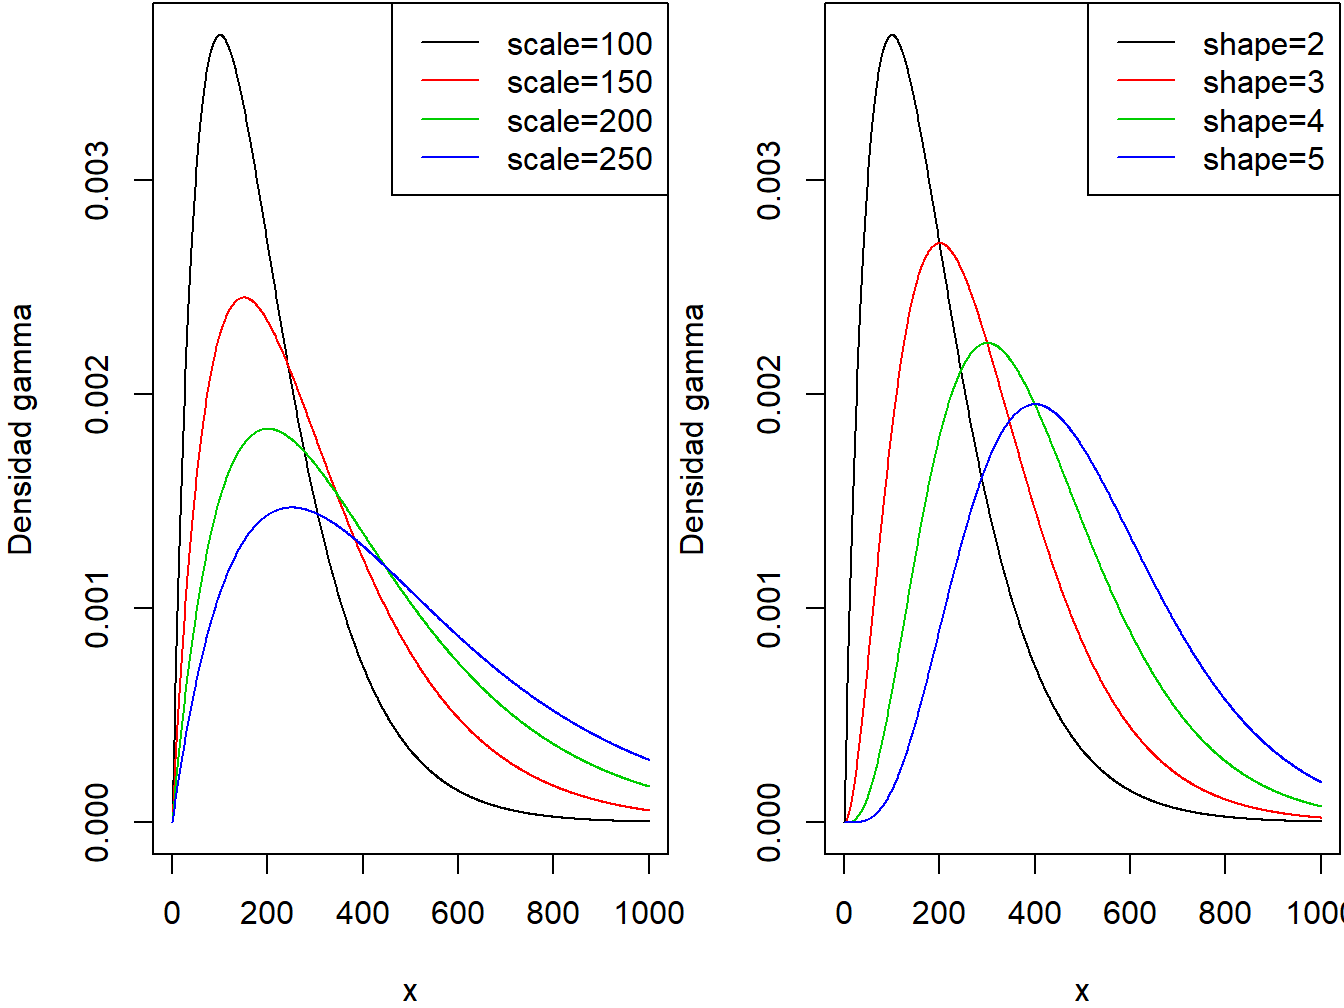
\includegraphics[width=1.2\linewidth]{LossDataAnalytics_files/figure-latex/gammapdf-1} 

}

\caption{Densidades Gamma. El panel de la izquierda corresponde a forma=2 y un parámetro de escala variable. 
 El panel de la derecha corresponde a escala=100 y parámetro de forma variable.}\label{fig:gammapdf}
\end{figure}

\begin{verbatim}
par(mfrow=c(1, 2), mar = c(4, 4, .1, .1))

# Densidades gamma con escala variable
scaleparam <- seq(100, 250, by = 50)
shapeparam <- 2:5
x <- seq(0, 1000, by = 1)
fgamma <- dgamma(x, shape = 2, scale = scaleparam[1])
plot(x, fgamma, type = "l", ylab = "Densidad gamma")
for(k in 2:length(scaleparam)){
  fgamma <- dgamma(x,shape = 2, scale = scaleparam[k])
  lines(x,fgamma, col = k)
}
legend("topright", c("scale=100", "scale=150", "scale=200", "scale=250"), lty=1, col = 1:4)

# Densidades gamma con forma variable
fgamma <- dgamma(x, shape = shapeparam[1], scale = 100)
plot(x, fgamma, type = "l", ylab = "Densidad gamma")
for(k in 2:length(shapeparam)){
  fgamma <- dgamma(x,shape = shapeparam[k], scale = 100)
  lines(x,fgamma, col = k)
}
legend("topright", c("shape=2", "shape=3", "shape=4", "shape=5"), lty=1, col = 1:4)
\end{verbatim}

Cuando \(\alpha = 1\) la gamma se reduce a una distribución exponencial y cuando \(\alpha = \frac{n}{2}\) y \(\theta = 2\) la gamma se reduce a una distribucióin chi-cuadrado con \(n\) grados de libertad. Tal y como veremos en la Sección \ref{S:AppA:HT}, la distribución chi-cuadrado es ampliamente utilitzada en el contraste estadístico de hipótesis.

La función de distribución de un modelo gamma es la función incompleta gamma, denotada por \(\Gamma\left(\alpha; \frac{x}{\theta} \right)\), y definida como
\[
F_{X}\left( x \right) = \Gamma\left( \alpha; \frac{x}{\theta} \right) = \frac{1}{\Gamma\left( \alpha \right)}\int_{0}^{x /\theta}t^{\alpha - 1}e^{- t}~dt
\]
\(\alpha > 0,\ \theta > 0\). Para un entero \(\alpha\), puede expresarse como \(\Gamma\left( \alpha; \frac{x}{\theta} \right) = 1 - e^{-x/\theta}\sum_{k = 0}^{\alpha-1}\frac{(x/\theta)^k}{k!}\).

El momento \(k\)-ésimo de una variable aleatoria con distribución gamma para cualquier \(k\) positivo viene dada por
\[
\mathrm{E}\left( X^{k} \right) = \theta^{k} \frac{\Gamma\left( \alpha + k \right)}{\Gamma\left( \alpha \right)} .
\]
La media y varianza vienen dadas por \(\mathrm{E}\left( X \right) = \alpha\theta\) y \(\mathrm{Var}\left( X \right) = \alpha\theta^{2}\), respectivamente.

Dado que todos los momentos existen para cualquier \(k\) positivo, la distribución gamma se considera una distribución de cola ligera, que puede no ser adecuada para modelitzar activos con riesgo dado que no proporciona una valoración realista de la versimilitud de pérdidas severas.

\hypertarget{distribuciuxf3n-pareto}{%
\subsection{Distribución Pareto}\label{distribuciuxf3n-pareto}}

La distribución Pareto, denominada así por el economista italiano Vilfredo Pareto (1843-1923), tiene muchas aplicacions económicas y financieras. Es una distribución con asimetria positiva y con cola pesada que la hace adecuada para modelitzar ingresos, siniestros en seguros con alto riesgo y la severidad de grandes pérdidas en seguros. La función de supervivencia de una distribución de Pareto que decrece lentamente a cero fue por primera vez utilizada para describir la distribución de ingresos en los que un pequeño porcentaje de la población tiene una gran proporción de la riqueza total. Para siniestros extermos en seguros, la cola de la distribución de la severidad (pérdidas por encima de un determinado umbral) pueden modelizarse usando una distribución Pareto Generalizada.

Se dice que la variable continua \(X\) tiene una distribución de Pareto con parámetro de forma \(\alpha\) y parámetro de escala \(\theta\) si su \emph{pdf} viene dada por
\[
f_{X}\left( x \right) = \frac{\alpha\theta^{\alpha}}{\left( x + \theta \right)^{\alpha + 1}} \ \ \  x  >  0,\ \alpha >  0,\ \theta > 0.
\]
Los dos paneles de la Figura \ref{fig:Paretopdf} muestran los efectos de los parámetros de escala y forma en la función de densidad Pareto.

\begin{figure}

{\centering 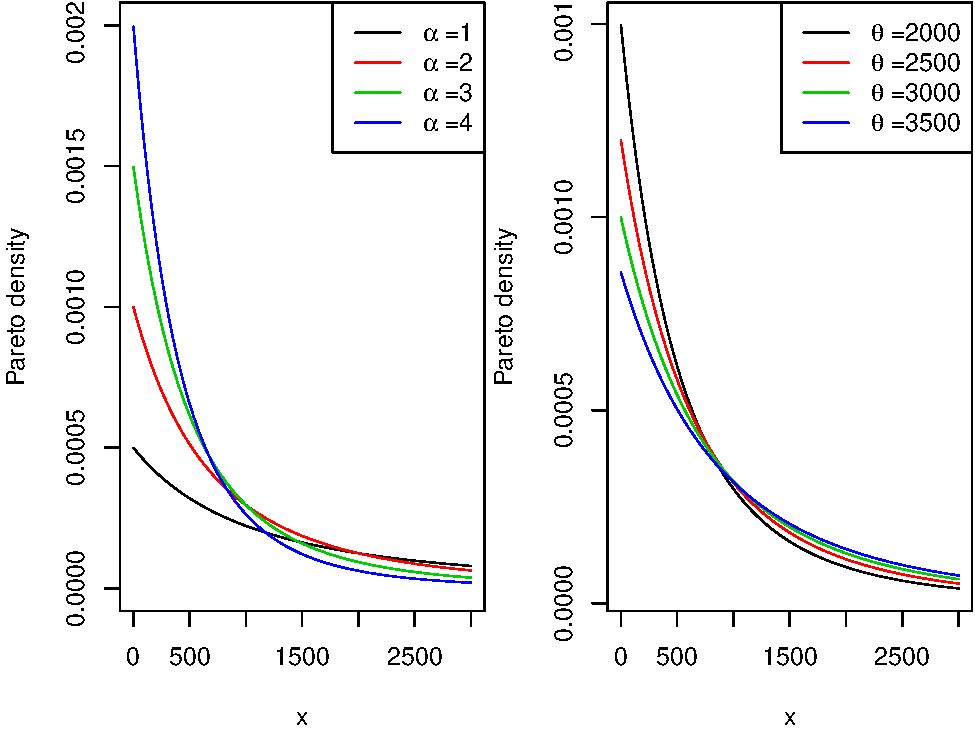
\includegraphics[width=1.2\linewidth]{LossDataAnalytics_files/figure-latex/Paretopdf-1} 

}

\caption{Densidades Pareto. El panel de la izquierda corresponde a escala=2000 y forma variable. El panel de la derecha corresponde a forma=3 y escala variable}\label{fig:Paretopdf}
\end{figure}

\begin{verbatim}
library(VGAM)

par(mfrow=c(1, 2), mar = c(4, 4, .1, .1))

# Densidades Pareto con forma variable
x <- seq(1, 3000, by = 1)
scaleparam <- seq(2000, 3500, 500)
shapeparam <- 1:4

# variando el parámetro de forma
plot(x, dparetoII(x, loc=0, shape = shapeparam[1], scale = 2000), ylim=c(0,0.002),type = "l", ylab = "Pareto density")
for(k in 2:length(shapeparam)){
  lines(x, dparetoII(x, loc=0, shape = shapeparam[k], scale = 2000), col = k)
}
legend("topright", c(expression(alpha~'=1'), expression(alpha~'=2'), expression(alpha~'=3'), expression(alpha~'=4')), lty=1, col = 1:4)

# Densidades de Pareto con escala variable
plot(x, dparetoII(x, loc=0, shape = 3, scale = scaleparam[1]), type = "l", ylab = "Pareto density")
for(k in 2:length(scaleparam)){
  lines(x, dparetoII(x, loc=0, shape = 3, scale = scaleparam[k]), col = k)
}
legend("topright", c(expression(theta~'=2000'), expression(theta~'=2500'), expression(theta~'=3000'), expression(theta~'=3500')), lty=1, col = 1:4)
\end{verbatim}

La función de distribución de una Pareto viene dada por
\[
F_{X}\left( x \right) = 1 - \left( \frac{\theta}{x + \theta} \right)^{\alpha}  \ \ \ x > 0,\ \alpha > 0,\ \theta > 0.
\]
Se puede ver fácilmente que la función de riesgo de la distribución de Pareto es una función decreciente en \(x\), otro indicador de que es una distribución de cola pesada. Cuando la función de riesgo decrece con el tiempo la población fallece a una tasa decreciente dando como resultado una cola más pesada para la distribución. La función de riesgo revela información sobre la distribución de la cola y es frecuentemente usada para modelizar distribuciones en análisis de la supervivencia. La función de riesgo se define como la posibilidad instantánea de que el evento de interés ocurra dentro de un marco temporal muy pequeño.

El momento \(k\)-ésimo de una variable aleatoria con una distribución de Pareto existe si y solo si \(\alpha > k\). Si \(k\) es un entero positivo entonces
\[
\mathrm{E}\left( X^{k} \right) = \frac{\theta^{k}~ k!}{\left( \alpha - 1 \right)\cdots\left( \alpha - k \right)} \ \ \ \alpha > k.
\]
La media y varianza vienen dadas por \[\mathrm{E}\left( X \right) = \frac{\theta}{\alpha - 1} \ \ \ \text{for } \alpha > 1\] y
\[\mathrm{Var}\left( X \right) = \frac{\alpha\theta^{2}}{\left( \alpha - 1 \right)^{2}\left( \alpha - 2 \right)} \ \ \ \text{for } \alpha > 2,\]respectivamente.

\textbf{Ejemplo 3.2.1. }
El tamaño de los siniestros en una cartera de asegurados sigue una distribución de Pareto con media y varianza iguales a 40 y 1800 respectivamente. Encuentra

Los parámetros de forma y escala.

El percentil 95 de la distribución.

\textbf{Solución.}

\textbf{a.} Dado que \(X\sim Pa(\alpha,\theta)\), se tiene que \(\mathrm{E}\left( X \right) = \frac{\theta}{\alpha - 1} = 40\) y
\(\mathrm{Var}\left( X \right) = \frac{\alpha\theta^{2}}{\left( \alpha - 1 \right)^{2}\left( \alpha - 2 \right)} = 1800\).
Dividiendo el cuadrado de la primera ecuación por la segunda obtenemos
\(\frac{\alpha - 2}{\alpha} = \frac{40^{2}}{1800}\). Por tanto, \(\alpha = 18,02\) y \(\theta = 680,72\).\\
\textbf{b.} El percentil 95, \(\pi_{0,95}\), satisface la ecuación
\[
F_{X}\left( \pi_{0,95} \right) = 1 - \left( \frac{680,72}{\pi_{0,95} + 680,72} \right)^{18,02} = 0,95.
\]
Por tanto, \(\pi_{0,95} = 122,96\).

\begin{center}\rule{0.5\linewidth}{0.5pt}\end{center}

\hypertarget{S:LS:Weibull}{%
\subsection{Distribución Weibull}\label{S:LS:Weibull}}

La distribución Weibull, denominada así por el físico sueco Waloddi Weibull (1887-1979) es ampliamente utilizada en fiabilidad, análisis de tiempos de vida, predicciones del tiempo y siniestros en seguros generales. Datos truncados aparecen frecuentemente en estudios de seguros. La distribución Weibull ha sido utilizada para modelizar el acuerdo de exceso de pérdida en el seguro del automóvil así como el tiempo entre la llegada de dos terremotos.

Se dice que la variable continua \(X\) sigue una distribución Weibull con parámetro de forma \(\alpha\) y parámetro de escala \(\theta\) si su función de densidad de probabilidad viene dada por
\[
f_{X}\left( x \right) = \frac{\alpha}{\theta}\left( \frac{x}{\theta} \right)^{\alpha - 1} \exp \left(- \left( \frac{x}{\theta} \right)^{\alpha}\right) \ \ \ x > 0,\ \alpha > 0,\ \theta > 0.
\]
Los dos paneles de la Figura \ref{fig:Weibullpdf} muestran los efectos de los parámetros de escala y forma de la función de densidad de una Weibull.

\begin{figure}

{\centering 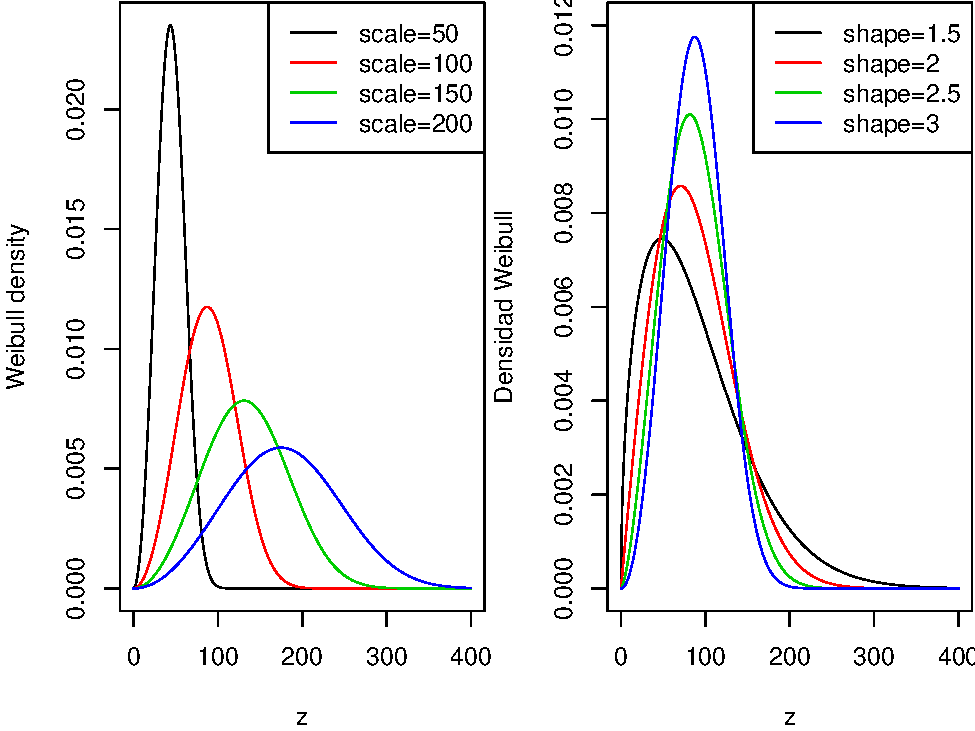
\includegraphics[width=1.2\linewidth]{LossDataAnalytics_files/figure-latex/Weibullpdf-1} 

}

\caption{Densidades Weibull. El panel de la izquierda corresponde a forma=3 y escala variable. El panel de la derecha corresponde a escala=100 y forma variable.}\label{fig:Weibullpdf}
\end{figure}

\begin{verbatim}
par(mfrow=c(1, 2), mar = c(4, 4, .1, .1))

# Densidad Weibull con escala variable
z<- seq(0,400,by=1)
scaleparam <- seq(50,200,50)
shapeparam <- seq(1.5,3,0.5)
plot(z, dweibull(z, shape = 3, scale = scaleparam[1]), type = "l", ylab = "Densidad Weibull")
for(k in 2:length(scaleparam)){
  lines(z,dweibull(z,shape = 3, scale = scaleparam[k]), col = k)}
legend("topright", c("scale=50", "scale=100", "scale=150", "scale=200"), lty=1, col = 1:4)

# Densidad Weibull con forma variable
plot(z, dweibull(z, shape = shapeparam[1], scale = 100), ylim=c(0,0.012), type = "l", ylab = "Densidad Weibull ")
for(k in 2:length(shapeparam)){
  lines(z,dweibull(z,shape = shapeparam[k], scale = 100), col = k)}
legend("topright", c("shape=1.5", "shape=2", "shape=2.5", "shape=3"), lty=1, col = 1:4)
\end{verbatim}

La función de distribución de una Weibull viene dada por
\[
F_{X}\left( x \right) = 1 - e^{- \left( x / \theta \right)^{\alpha}}  \ \ \ x >  0,\ \alpha >  0,\ \theta > 0.
\]

Se puede ver fácilmente que el parámetro de forma \(\alpha\) describe la forma de la función de riesgo de una distribución Weibull. La función de riesgo es una función decreciente cuando \(\alpha < 1\) (distribución de cola pesada), constante cuando \(\alpha = 1\) y creciente cuando \(\alpha > 1\) (distribución de cola ligera). Este comportamiento de la función de riesgo hace que la distribución de Weibull sea adecuada para una gran variedad de fenómenos como la predicción del tiempo, ingeniería eléctrica e industrial, modelización actuarial y análisis del riesgo financiero.

El momento \(k\)-ésimo de una variable aleatoria con distribución Weibull viene dado por
\[
\mathrm{E}\left( X^{k} \right) = \theta^{k}~\Gamma\left( 1 + \frac{k}{\alpha} \right) .
\]

La media y la varianza vienen dades por
\[
\mathrm{E}\left( X \right) = \theta~\Gamma\left( 1 + \frac{1}{\alpha} \right)
\]
y
\[
\mathrm{Var}(X)= \theta^{2}\left( \Gamma\left( 1 + \frac{2}{\alpha} \right)  - \left\lbrack \Gamma\left( 1 + \frac{1}{\alpha} \right) \right\rbrack  ^{2}\right),
\]
respectivamente.

\textbf{Ejemplo 3.2.2.}
Se asume que la distribución de probabilidad del tiempo de vida de pacientes con SIDA (en meses) desde el momento del diagnóstico sigue una distribución de Weibull con parámetro de forma 1,2 y parámetro de escala 33,33.

Determina la probabilidad de que una persona de esta población elegida al azar sobreviva al menos 12 meses,

Se selecciona una muestra de 10 pacientes de esta población. Cuál es la probabilidad de que como máximo dos mueran al cabo de un año del diagnóstico.

Encuentra el percentil 99 de la distribución de los tiempos de vida.

\textbf{Solución.}

\textbf{a.} Sea \(X\) el tiempo de vida de los pacientes con SIDA (en meses) con distribución Weibull de parámetros \(\left(1,2,\ 33,33 \right)\). Tenemos,

\[
\Pr \left( X \geq 12 \right) = S_{X} \left( 12 \right) = e^{- \left( \frac{12}{33,33} \right)^{1,2}} = 0,746.
\]

\textbf{b.} Sea \(Y\) el número de pacientes que mueren al cabo de un año del diagnóstico. Entonces, \(Y\sim Bin\left( 10,\ 0,254 \right)\) y \(\Pr\left( Y \leq 2 \right) = 0,514.\)

\textbf{c.} Sea \(\pi_{0,99}\) el percentil 99 de esta distribución. Entonces,
\[
S_{X}\left( \pi_{0,99} \right) = \exp\left\{- \left( \frac{\pi_{0,99}}{33,33} \right)^{1,2}\right\} = 0,01.
\]
Resolviendo para \(\pi_{0,99}\), obtenemos \(\pi_{0,99} = 118,99\).

\begin{center}\rule{0.5\linewidth}{0.5pt}\end{center}

\hypertarget{distribuciuxf3n-beta-generalizada-de-segundo-tipo}{%
\subsection{Distribución Beta Generalizada de segundo tipo}\label{distribuciuxf3n-beta-generalizada-de-segundo-tipo}}

La Distribución Beta Generalizada de segundo tipo (\emph{GB2}) fue introducida por \citet{venter1983transformed} en el contexto de la modelización de las pérdidas en seguros y por \citet{mcdonald1984some} como una distribución para los ingresos y la riqueza. Es una distribución de cuatro parámetros muy flexible que puede modelizar distribuciones con asimetria tanto positiva como negativa.

Se dice que la variable \(X\) tiene una distribución \emph{GB2} con parámetros \(\sigma\), \(\theta\), \(\alpha_1\) y \(\alpha_2\) si su función de densidad de probabilidad viene dada por

\begin{equation}
f_{X}\left( x \right) = \frac{(x/\theta)^{\alpha_2/\sigma}}{x \sigma~\mathrm{B}\left( \alpha_1,\alpha_2\right)\left\lbrack 1 + \left( x/\theta \right)^{1/\sigma} \right\rbrack^{\alpha_1 + \alpha_2}} \ \ \ \text{for } x > 0,
  \label{eq:GB2Distn}
\end{equation}

\(\sigma,\theta,\alpha_1,\alpha_2 > 0\), y donde la función beta es \(\mathrm{B}\left( \alpha_1,\alpha_2 \right)\) definida como
\[
\mathrm{B}\left( \alpha_1,\alpha_2\right) = \int_{0}^{1}{t^{\alpha_1 - 1}\left( 1 - t \right)^{\alpha_2 - 1}}~ dt.
\]

La \emph{GB2} proporciona una modelo para datos con cola pesada así como ligera. Incluye a las distribuciones exponencial, gamma, Weibull, Burr, Lomax, F, chi-cuadrado, Rayleigh, lognormal y log-logistic como casos especiales o límite. Por ejemplo, estableciendo estos valores para los parámetros \(\sigma = \alpha_1 = \alpha_2 = 1\), la \emph{GB2} se reduce a la distribución log-logistic. Cuando \(\sigma = 1\) y \(\alpha_2 \rightarrow \infty\), se reduce a la distribución gamma y cuando \(\alpha = 1\) y \(\alpha_2 \rightarrow \infty\), se reduce a la distribución Weibull.

Una variable aleatoria \emph{GB2} puede ser definida como sigue. Se asume que \(G_1\) y \(G_2\) son variables aleatorias independientes donde \(G_i\) tiene una distribución gamma con parámetros \(\alpha_i\) y parámetro de escala igual a 1. Entonces, puede demostrarse que la variable aleatoria \(X = \theta \left(\frac{G_1}{G_2}\right)^{\sigma}\) sigue una distribución \emph{GB2} con \emph{pdf} resumida en la ecuación \eqref{eq:GB2Distn}. Este resultado teórico tiene diverses implicaciones. Por ejemplo, cuando los momentos existen, puede demostrarse que el momento \(k\)-ésimo de la variable aleatoria con distribución \emph{GB2} viene dado por
\[
\mathrm{E}\left( X^{k} \right) = \frac{\theta^{k}~\mathrm{B}\left( \alpha_1 +k \sigma,\alpha_2 - k \sigma \right)}{\mathrm{B}\left( \alpha_1,\alpha_2 \right)}, \ \ \ k > 0.
\]

Anteriormente la \emph{GB2} también había sido aplicada a datos de ingresos y más recientemente ha sido utilitzada para modelitzar datos de siniestros de cola larga (en la Sección \ref{S:Tails} se describen diferentes interpretaciones del concepto ``cola larga''). \emph{GB2} fue usada para modelizar diferentes tipos de siniestros en el seguro del automóvil, severidad de las pérdidas causades por el fuego así como datos de sinietros en seguros médicos.

\hypertarget{MethodsCreation}{%
\section{Métodos para Crear Distribuciones Nuevas}\label{MethodsCreation}}

\begin{center}\rule{0.5\linewidth}{0.5pt}\end{center}

En esta sección se mostrara como:

\begin{itemize}
\tightlist
\item
  Entender las conexiones entre distribuciones
\item
  Proporcionar ideas sobre cuando una distribución es preferible en comparación con otras alternativas
\item
  Proporcionar los fundamentos para la creación de nuevas distribuciones
\end{itemize}

\begin{center}\rule{0.5\linewidth}{0.5pt}\end{center}

\hypertarget{funciones-de-variables-aleatorias-y-sus-distribuciones}{%
\subsection{Funciones de variables aleatorias y sus distribuciones}\label{funciones-de-variables-aleatorias-y-sus-distribuciones}}

En la Sección \ref{S:ContinuousDistn} se han descrito algunas distribuciones fundamentales conocidas. En esta sección se describe la forma de crear nuevas distribuciones de probabilidad paramétricas a partir de otras existentes. Concretamente, sea \(X\) una variable aleatoria continua con función de densidad de probabilidad conocida \(f_{X}(x)\) y función de distribución \(F_{X}(x)\). Se desea conocer la distribución de \(Y = g\left( X \right)\), donde \(g(X)\) es una transformación uno-a-uno que define una nueva variable aleatoria \(Y\). Es esta sección se aplica las siguientes técnicas para crear nuevas familias de distribuciones: (a) multiplicación por una constante (b) elevación a una potencia, (c) exponenciación y (d) mixtura.

\hypertarget{multiplicaciuxf3n-por-una-constante}{%
\subsection{Multiplicación por una constante}\label{multiplicaciuxf3n-por-una-constante}}

Si los datos de siniestros muestran cambios a lo largo del tiempo entonces esta transformación puede ser útil para ajustar el efecto de la inflación. Si el nivel de la inflación es positivo entonces los costes de los siniestros están aumentando, y si es negativo los costes están decreciendo. Para realizar el ajuste por inflación multiplicamos el coste \(X\) por 1+ tasa de inflación (inflación negativa es deflacción). Para tener en cuenta el impacto de los tipos de cambio en los costes de los siniestros también usamos una transformación para aplicar la conversión de una moneda base a otra.

Se considera la transformación \(Y = cX\), donde \(c > 0\), entonces, la función de distribución de \(Y\) viene dada por
\[
F_{Y}\left( y \right) = \Pr\left( Y \leq y \right) = \Pr\left( cX \leq y \right) = \Pr\left( X \leq \frac{y}{c} \right) = F_{X}\left( \frac{y}{c} \right).
\]
Por lo tanto, la función de densidad de probabilidad que se desea determinar \(f_{Y}(y)\) puede expresarse como
\[
f_{Y}\left( y \right) = \frac{1}{c}f_{X}\left( \frac{y}{c} \right).
\]
Se asume que \(X\) pertenece a un cierto conjunto de distribuciones paramétricas y se define la versión reescalada \(Y\  = \ cX\), \(c\  > \ 0\). Si \(Y\) está en el mismo conjunto de distribuciones entonces se dice que la distribución es una distribución escala. Cuando un miembro de una distribución escala se multiplica por una constante \(c\) (\(c > 0\)), el parámetro de escala de esa distribución escala cumple dos condiciones:

El parámetro se transforma multiplicando por \(c\);

El resto de parámetros no se ven afectados.

\textbf{Ejemplo 3.3.1. Pregunta de un examen actuarial.}
Las pérdidas agregadas de Eiffel Auto Insurance se denotan en Euros y siguen una distribución lognormal con \(\mu = 8\) y \(\sigma = 2\). Dado que 1 euro \(=\) 1,3 dólares, encuentra el conjunto de parámetros lognormales que describen la distribución de pérdidas de Eiffel en dólares.

\textbf{Solución.}

Sean \(X\) e \(Y\) las pérdidas agregadas de Eiffel Auto Insurance en euros y dólares respectivamente. Dado que \(Y = 1.3X\), tenemos,
\[
F_{Y}\left( y \right) = \Pr\left( Y \leq y \right) = \Pr\left( 1.3X \leq y \right) = \Pr\left( X \leq \frac{y}{1,3} \right) = F_{X}\left( \frac{y}{1.3} \right).
\]

\(X\) sigue una distribución lognormal con parámetros \(\mu = 8\) y \(\sigma = 2\). La función de densidad de probabilidad de \(X\) viene dada por
\[
f_{X}\left( x \right) = \frac{1}{x \sigma \sqrt{2\pi}}\exp \left\{- \frac{1}{2}\left( \frac{\ln x - \mu}{\sigma} \right)^{2}\right\} \ \ \ \text{para } x > 0.
\]
Dado que \(\left| \frac{dx}{dy} \right| = \frac{1}{1,3}\), la función de densidad de probabilidad de interés \(f_{Y}(y)\) es
\[
f_{Y}\left( y \right) = \frac{1}{1,3}f_{X}\left( \frac{y}{1,3} \right) \\
= \frac{1}{1,3}\frac{1,3}{y \sigma \sqrt{2\pi}}\exp \left\{- \frac{1}{2}\left( \frac{\ln\left( y/1.3 \right) - \mu}{\sigma} \right)^{2}\right\} \\
= \frac{1}{y \sigma\sqrt{2\pi}}\exp \left\{- \frac{1}{2}\left( \frac{\ln y - \left( \ln 1,3 + \mu \right)}{\sigma} \right)^{2}\right\}.
\]
Entonces \(Y\) sigue una distribución lognormal con parámetros \(\ln 1,3 + \mu = 8,26\) y \(\sigma = 2,00\). Si se establece que \(\mu = ln(m)\) entonces resulta fácil ver que \(m\)=\(e^{\mu}\) es el parámetro de escala que fue multiplicado por 1,3 mientras que \(\sigma\) es el parámetro de forma que no se ha visto alterado.

\begin{center}\rule{0.5\linewidth}{0.5pt}\end{center}

\textbf{Ejemplo 3.3.2. Pregunta de un examen actuarial.}
Demuestra que la distribución gamma es una distribución escala.

\textbf{Solución.}

Sea \(X\sim Ga(\alpha,\theta)\) e \(Y = cX\). Dado que \(\left| \frac{dx}{dy} \right| = \frac{1}{c}\), entonces
\[
f_{Y}\left( y \right) = \frac{1}{c}f_{X}\left( \frac{y}{c} \right) = \frac{\left( \frac{y}{c\theta} \right)^{\alpha}}{y~\Gamma\left( \alpha \right)}\exp \left( - \frac{y}{c\theta} \right)  .
\]
Se puede ver que \(Y\sim Ga(\alpha,c\theta)\) lo cual indica que la gamma es una distribución escala y \(\theta\) es un parámetro de escala.

Usando el mismo enfoque podemos demostrar que otras distribuciones introducidas en la Sección \ref{S:ContinuousDistn} son también distribuciones escala. En la modelización actuarial, trabajar con una distribución escala es muy conveniente porque permite incorporar el efecto de la inflación y adaptar los cambios en la modeda correspondiente.

\begin{center}\rule{0.5\linewidth}{0.5pt}\end{center}

\hypertarget{elevaciuxf3n-a-una-potencia}{%
\subsection{Elevación a una potencia}\label{elevaciuxf3n-a-una-potencia}}

En la Sección \ref{S:LS:Weibull} se ha tratado la fexibilidad de la distribución de Weibull para el ajuste de datos de fiabilidad. Teniendo en cuenta los orígenes de la distribución de Weibull, se reconoce que la Weibull es una transformación basada en la potencia de la distribución exponencial. Esta se una aplicación de otro tipo de transformación que implica elevar una variable aleatoria a una potencia.

Si se considera la transformación \(Y = X^{\tau}\), donde \(\tau > 0\), entonces la función de distribución de \(Y\) viene dada por
\[
F_{Y}\left( y \right) = \Pr\left( Y \leq y \right) = \Pr\left( X^{\tau} \leq y \right) = \Pr\left( X \leq y^{1/ \tau} \right) = F_{X}\left( y^{1/ \tau} \right).
\]

Por lo tanto, la función de densidad de probabilidad de interés \(f_{Y}(y)\) puede expresarse como
\[
f_{Y}(y) = \frac{1}{\tau} y^{1/ \tau - 1} f_{X}\left( y^{1/ \tau} \right).
\]
Por otro lado, si \(\tau < 0\), la función de distribución de \(Y\) viene dada por
\[
F_{Y}\left( y \right) = \Pr\left( Y \leq y \right) = \Pr\left( X^{\tau} \leq y \right) = \Pr\left( X \geq y^{1/ \tau} \right) = 1 - F_{X}\left( y^{1/ \tau} \right), 
\]
y
\[
f_{Y}(y) = \left| \frac{1}{\tau} \right|{y^{1/ \tau - 1}f}_{X}\left( y^{1/ \tau} \right).
\]

\textbf{Ejemplo 3.3.3.}
Se asume que \(X\) sigue una distribución exponencial con media \(\theta\) y se considera la variable transformada \(Y = X^{\tau}\). Demuestra que \(Y\) sigue una distribución de Weibull cuando \(\tau\) es positiva y determina los parámetros de la distribución de Weibull.

\textbf{Solución.}

Dado que \(X\) sigue una distribución exponencial con media \(\theta\), tenemos
\[
f_{X}(x) = \frac{1}{\theta}e^{- x/ \theta} \ \ \ \, x > 0.
\]
Resolviendo para \emph{x} se obtiene \(x = y^{1/\tau}\). Tomando derivadas, tenemos
\[
\left| \frac{dx}{dy} \right| = \frac{1}{\tau}{y^{\frac{1}{\tau}-1}}.
\]
Así tenemos,
\[
f_{Y}\left( y \right) = \frac{1}{\tau}{y^{\frac{1}{\tau} - 1}f}_{X}\left( y^{\frac{1}{\tau}} \right) \\
= \frac{1}{\tau \theta }y^{\frac{1}{\tau} - 1}e^{- \frac{y^{\frac{1}{\tau}}}{\theta}} = \frac{\alpha}{\beta}\left( \frac{y}{\beta} \right)^{\alpha - 1}e^{- \left( y/ \beta \right)^{\alpha}}.
\]
donde \(\alpha = \frac{1}{\tau}\) y \(\beta = \theta^{\tau}\). Entonces, \(Y\) sigue una distribución de Weibull con parámetro de forma \(\alpha\) y parámetro de escala \(\beta\).

\begin{center}\rule{0.5\linewidth}{0.5pt}\end{center}

\hypertarget{exponenciaciuxf3n}{%
\subsection{Exponenciación}\label{exponenciaciuxf3n}}

La distribución normal es un modelo muy popular para un gran número de aplicaciones y cuando el tamaño muestral es grande, puede servir como una distribucion aproximada para otros modelos. Si una variable aleatoria \(X\) tiene una distribución normal con media \(\mu\) y varianza \(\sigma^{2}\), entonces \(Y = e^{X}\) tiene una distribución lognormal con parámetros \(\mu\) y \(\sigma^{2}\). La variable aleatoria lognormal está acotada en cero por abajo, tiene asimetria positiva y tiene una larga cola por la derecha. La distribución lognormal es frecuentemente utilizada para describir la distribución de activos financieros como los precios de las acciones. También es usada para ajustar cuantías de siniestros en los seguros del automóvil y de salud. Este es un ejemplo de otro tipo de transformación que implica exponenciación.

En general, consideramos la transformación \(Y = e^{X}\). Entonces, la función de distribución de \(Y\) viene dada por
\[F_{Y}\left( y \right) = \Pr\left( Y \leq y \right) = \Pr\left( e^{X} \leq y \right) = \Pr\left( X \leq \ln y \right) = F_{X}\left( \ln y \right).\]
Tomando derivadas, vemos que la función de densidad de probabilidad de interés \(f_{Y}(y)\) puede expresarse como
\[
f_{Y}(y) = \frac{1}{y}f_{X}\left( \ln y \right).
\]
Como un caso especial e importante, se asume que \(X\) tiene distribución normal con media \(\mu\) y varianza \(\sigma^2\). Entonces, la distribución de \(Y = e^X\) es

\[
f_{Y}(y) = \frac{1}{y}f_{X}\left( \ln y \right)
= \frac{1}{y\sqrt{2 \pi}} \exp \left\{-\frac{1}{2}\left(\frac{ \ln y - \mu}{\sigma}\right)^2\right\}. 
\]
A esta distribución se la conoce como la distribución \emph{lognormal}.

\textbf{Ejemplo 3.3.4. Pregunta de examen actuarial.}
Se asume que \(X\) tiene una distribución uniforme en el intervalo \((0,\ c)\) y definimos \(Y = e^{X}\). Determina la distribución de \(Y\).

\textbf{Solución.}

En primer lugar, se considera la \emph{cdf} de \(Y\),
\[
F_{Y}\left( y \right) = \Pr\left( Y \leq y \right) = \Pr\left( e^{X} \leq y \right) = \Pr\left( X \leq \ln y \right) = F_{X}\left( \ln y \right).
\]
Tomando derivadas, se tiene,
\[
f_{Y}\left( y \right) = \frac{1}{y}f_{X}\left(\ln y \right) = \frac{1}{cy} .
\]
Dado que \(0 < x < c\), entonces \(1 < y < e^{c}\).

\begin{center}\rule{0.5\linewidth}{0.5pt}\end{center}

\hypertarget{mixturas-finitas}{%
\subsection{Mixturas finitas}\label{mixturas-finitas}}

Las distribuciones mixtas representan una forma útil de modelizar datos que provienen de una población heterogénea. Esta población de origen puede considerarse dividida en múltiples subpoblaciones con diferentes distribuciones.

\hypertarget{mixtura-de-dos-variables}{%
\subsubsection{Mixtura de dos variables}\label{mixtura-de-dos-variables}}

Si el fenómeno subyacente es diverso y puede ser ciertamente descrito como dos fenómenos que representan dos subpoblaciones con diferentes modelos, es posible construir la variable aleatoria de mixtura de dos variables \(X\). Sean las variables aleatorias \(X_{1}\) y \(X_{2}\), con funciones de densidad de probabilidad \(f_{X_{1}}\left( x \right)\) y \(f_{X_{2}}\left( x \right)\) respectivamente, la función de densidad de probabilidad de \(X\) es la media ponderada de la componente de la funcion de densidad de probabilidad \(f_{X_{1}}\left( x \right)\) y \(f_{X_{2}}\left( x \right)\). Las funciones de densidad de probabilidad y de distribución de \(X\) vienen dadas por
\[f_{X}\left( x \right) = af_{X_{1}}\left( x \right) + \left( 1 - a \right)f_{X_{2}}\left( x \right),\]
y
\[F_{X}\left( x \right) = aF_{X_{1}}\left( x \right) + \left( 1 - a \right)F_{X_{2}}\left( x \right),\]

para \(0 < a <1\), donde los parámetros de mixtura \(a\) y \((1 - a)\) representan las proporciones de las observaciones de los datos que caen en cada una de las dos subpoblaciones repectivamente. Esta media ponderada puede ser aplicada a un buen número distribuciones relacionadas con cuantías. El momento \emph{k}-ésimo y la función generatriz de momentos de \(X\) vienen dadas por
\(\mathrm{E}\left( X^{k} \right) = a\mathrm{E}\left( X_{1}^{K} \right) + \left( 1 - a \right)\mathrm{E}\left( X_{2}^{k} \right)\),
y
\[M_{X}(t) = aM_{X_{1}}(t) + \left( 1 - a \right)M_{X_{2}}(t),\] respectivamente.

\textbf{Ejemplo 3.3.5. Pregunta del examen actuarial.}
En un conjunto de pólizas de seguros se distinguen dos tipos. 25\% de las pólizas son de Tipo 1 y 75\% de Tipo 2. Para una póliza de Tipo 1, la cuantía de pérdida por año sigue una distribución exponencial con media 200, y para las pólizas de Tipo 2, la cuantía de perdidas por año sigue una distribución de Pareto con parámetros \(\alpha=3\) y \(\theta=200\). Para una póliza seleccionada al azar de la población total que incluye los dos tipos de pólizas, encuentra la probabilidad de que la pérdida anual sea inferior a 100, y determina la perdida media.

\textbf{Solución.}

Los dos tipos de pérdidas son las variables aleatorias \(X_1\) y \(X_2\). \(X_1\) digue una distribución exponencial con media 100, por lo tanto \(F_{X_1}\left(100\right)=1-e^{-\frac{100}{200}}=0,393\). \(X_2\) sigue una distribución de Pareto con parámetros \(\alpha=3\) y \(\theta=200\), por lo tanto \(F_{X_1}\left(100\right)=1-\left(\frac{200}{100+200}\right)^3=0,704\). Por lo tanto, \(F_X\left(100\right)=\left(0,25\times0,393\right)+\left(0,75\times0,704\right)=0,626\).

La pérdida media viene dada por
\[\mathrm{E}\left(X\right)=0,25\mathrm{E}\left(X_1\right)+0,75\mathrm{E}\left(X_2\right)=\left(0,25\times200\right)+\left(0,75\times100\right)=125\].

\begin{center}\rule{0.5\linewidth}{0.5pt}\end{center}

\hypertarget{mixtura-de-k-variables}{%
\subsubsection{\texorpdfstring{Mixtura de \emph{k} variables}{Mixtura de k variables}}\label{mixtura-de-k-variables}}

En el caso de las distribuciones mixtas finitas, la variable aleatoria de interés \(X\) tiene una probabilidad \(p_{i}\) de provenir de una subpoblación homogénea \(i\), donde \(i = 1,2,\ldots,k\) y \(k\) es el número inicialment especificado de subpoblaciones en la mixtura. El parámetro de mixtura \(p_{i}\) representa la proporción de observaciones de la subpoblación \(i\). Se considera la variable aleatoria \(X\) que es generada por \(k\) subpoblaciones diferentes, donde la subpoblación \(i\) es modelizada con la distribución continua \(f_{X_{i}}\left( x \right)\). La distribución de probabilidad de \(X\) viene dada por
\[f_{X}\left( x \right) = \sum_{i = 1}^{k}{p_{i}f_{X_{i}}\left( x \right)},\]
donde \(0 < p_{i} < 1\) y \(\sum_{i = 1}^{k} p_{i} = 1\).

Este modelo es frecuentemente referenciado como mixtura finita o mixtura de \(k\) variables. La función de distribución, momento \(r\)-ésimo y funciones generatrices de momentos de la mixtura de \(k\) variables vienen dadas por

\[F_{X}\left( x \right) = \sum_{i = 1}^{k}{p_{i}F_{X_{i}}\left( x \right)},\]
\[\mathrm{E}\left( X^{r} \right) = \sum_{i = 1}^{k}{p_{i}\mathrm{E}\left( X_{i}^{r} \right)}, \text{and}\]
\[M_{X}(t) = \sum_{i = 1}^{k}{p_{i}M_{X_{i}}(t)},\] respectivamente.

\textbf{Ejemplo 3.3.6. Pregunta de un examen actuarial.}
\(Y_{1}\) es una mixtura de \(X_{1}\) y \(X_{2}\) con ponderaciones de mixtura \(a\) y \((1 - a)\). \(Y_{2}\) es una mixtura de \(X_{3}\) y \(X_{4}\) con ponderaciones de mixtura \(b\) y \((1 - b)\). \(Z\) es una mixtura de \(Y_{1}\) y \(Y_{2}\) con ponderaciones de mixtura \(c\) y \((1 - c)\).

Demuestra que \(Z\) es una mixtura de \(X_{1}\), \(X_{2}\), \(X_{3}\) y \(X_{4}\), y determina las ponderaciones de mixtura.

\textbf{Solución.}
Aplicando la fórmula para una distribución mixta, obtenemos
\[f_{Y_{1}}\left( x \right) = af_{X_{1}}\left( x \right) + \left( 1 - a \right)f_{X_{2}}\left( x \right)\]

\[f_{Y_{2}}\left( x \right) = bf_{X_{3}}\left( x \right) + \left( 1 - b \right)f_{X_{4}}\left( x \right)\]

\[f_{Z}\left( x \right) = cf_{Y_{1}}\left( x \right) + \left( 1 - c \right)f_{Y_{2}}\left( x \right)\]

Sustituyendo las dos primeras ecuaciones en la tercera, obtenemos

\[f_{Z}\left( x \right) = c\left\lbrack af_{X_{1}}\left( x \right) + \left( 1 - a \right)f_{X_{2}}\left( x \right) \right\rbrack + \left( 1 - c \right)\left\lbrack bf_{X_{3}}\left( x \right) + \left( 1 - b \right)f_{X_{4}}\left( x \right) \right\rbrack\]

\[= caf_{X_{1}}\left( x \right) + c\left( 1 - a \right)f_{X_{2}}\left( x \right) + \left( 1 - c \right)bf_{X_{3}}\left( x \right) + (1 - c)\left( 1 - b \right)f_{X_{4}}\left( x \right)\].

Entonces, \(Z\) es una mixtura de \(X_{1}\), \(X_{2}\), \(X_{3}\) y \(X_{4}\), con pesos de mixtura \(\text{ca}\), \(c\left( 1 - a \right)\), \(\left( 1 - c \right)b\) y \((1 - c)\left( 1 - b \right)\), respectivamente. Se puede ver fácilmente que las ponderaciones de mixtura suman uno.

\begin{center}\rule{0.5\linewidth}{0.5pt}\end{center}

\hypertarget{mixturas-continuas}{%
\subsection{Mixturas continuas}\label{mixturas-continuas}}

Una mixtura con un gran número de subpoblaciones (\(k\) tiende a infinito) es frecuentemente denominada mixtura continua. En una mixtura continua, las subpoblaciones no se distinguen a través de un parámetro de mixtura discreto sino por una variable continua \(\Theta\), donde \(\Theta\) juega el papel de \(p_{i}\) en la mixtura finita. Se considera la variable aleatoria \(X\) con una distribución que depende de un parametro \(\Theta\), donde \(\Theta\) es a su vez una variable aleatoria continua. Esta descrición da lugar al siguiente modelo para \(X\)
\[
f_{X}\left( x \right) = \int_{-\infty}^{\infty}{f_{X}\left(x \left| \theta \right.  \right)g_{\Theta}( \theta )} d \theta ,
\]
donde \(f_{X}\left( x | \theta \right)\) es la distribución condicional de \(X\) en un valor concreto de \(\Theta=\theta\) y \(g_{\Theta}\left( \theta \right)\) es la declaración realitzada sobre la probabilidad en relación con el parámetro \(\theta\) desconocido. En un contexto Bayesiano (descrito en la Sección \ref{S:MS:BayesInference}), se le conoce como la distribución a priori de \(\Theta\) (la información a priori u opinión experta que se va a utilitzar en el análisis).

La función de distribución, momento \(k\)-ésimo y función generatriz de momentos de la mixtura continua vienen dadas por
\[
F_{X}\left( x \right) = \int_{-\infty}^{\infty}{F_{X}\left(x \left| \theta \right.  \right) g_{\Theta}(\theta)} d \theta,
\]
\[
\mathrm{E}\left( X^{k} \right) = \int_{-\infty}^{\infty}{\mathrm{E}\left( X^{k}\left| \theta \right.  \right)g_{\Theta}(\theta)}d \theta,
\]
\[
M_{X}(t) = \mathrm{E}\left( e^{t X} \right) = \int_{-\infty}^{\infty}{\mathrm{E}\left( e^{ tx}\left| \theta \right.  \right)g_{\Theta}(\theta)}d \theta, 
\]
respectivamente.

El momento \(k\)-ésimo de la distribución mixta puede ser igualmente expresado como
\[
\mathrm{E}\left( X^{k} \right) = \int_{-\infty}^{\infty}{\mathrm{E}\left( X^{k}\left| \theta \right.  \right)g_{\Theta}(\theta)}d\theta ~=~ \mathrm{E}\left\lbrack \mathrm{E}\left( X^{k}\left| \Theta \right.  \right) \right\rbrack .
\]

Usando la ley de las esperanzas iteradas (ver Apéndice Capítulo \ref{C:AppB}), se puede definir la media y varianza de \(X\) como
\[
\mathrm{E}\left( X \right) = \mathrm{E}\left\lbrack \mathrm{E}\left( X\left| \Theta \right.  \right) \right\rbrack
\]
y
\[
\mathrm{Var}\left( X \right) = \mathrm{E}\left\lbrack \mathrm{Var}\left( X\left| \Theta \right.  \right) \right\rbrack + \mathrm{Var}\left\lbrack \mathrm{E}\left( X\left| \Theta \right.  \right) \right\rbrack .
\]

\textbf{Ejemplo 3.3.7. Pregunta del examen actuarial.}
\(X\) tiene una distribución normal con media \(\Lambda\) y varianza 1. \(\Lambda\) tiene una distribución normal con media 1 y varianza 1. Determina la media y varianza de \(X\).

\textbf{Solución.}

X es una mixtura continua con media

\[
\mathrm{E}\left(X\right)=\mathrm{E}\left[\mathrm{E}\left(X\middle|\Lambda\right)\right]=\mathrm{E}\left(\Lambda\right)=1 \text{ and } \mathrm{V}\left(X\right)=\mathrm{V}\left[\mathrm{E}\left(X\middle|\Lambda\right)\right]+\mathrm{E}\left[\mathrm{V}\left(X\middle|\Lambda\right)\right]=\mathrm{V}\left(\Lambda\right)+\mathrm{E}\left(1\right)=1+1=2.
\]

\begin{center}\rule{0.5\linewidth}{0.5pt}\end{center}

\textbf{Ejemplo 3.3.8. Pregunta del examen actuarial.}
Las cuantías de los siniestros, \(X\), son uniformes en el intervalo \(\left(\Theta,\Theta+10\right)\) para cada asegurado. \(\Theta\) varía según el asegurado de acuerdo a una distribución exponencial con media 5. Determina la distribución incondicional, media y varianza de \(X\).

\textbf{Solución.}

La distribución condicional de \(X\) es \(f_{X}\left( \left. \ x \right|\theta \right) = \frac{1}{10}\) para \(\theta < x < \theta + 10\).

La distribución a priori de \(\theta\) es \(g_{\Theta}(\theta) = \frac{1}{5}e^{- \frac{\theta}{5}}\) para \(0 < \theta < \infty\).

La media y varianza condicionales de \(X\) vienen dadas por
\[
\mathrm{E}\left( \left. \ X \right|\theta \right) = \frac{\theta + \theta + 10}{2} = \theta + 5
\]
y
\[
\mathrm{Var}\left( \left. \ X \right|\theta \right) = \frac{\left\lbrack \left( \theta + 10 \right) - \theta \right\rbrack^{2}}{12} = \frac{100}{12}, 
\]
respectivamente.

Por lo tanto, la media y varianza incondicionales de \(X\) vienen dadas por

\[
\mathrm{E}\left( X \right) = \mathrm{E}\left\lbrack \mathrm{E}\left( X\left| \Theta \right.  \right) \right\rbrack = \mathrm{E}\left( \Theta + 5 \right) = \mathrm{E}\left( \Theta \right) + 5 = 5 + 5 = 10,
\]

y

\[
\mathrm{Var}\left( X \right) = \mathrm{E}\left\lbrack V\left( X\left| \Theta \right.  \right) \right\rbrack + \mathrm{Var}\left\lbrack \mathrm{E}\left( X\left| \Theta \right.  \right) \right\rbrack \\
= \mathrm{E}\left( \frac{100}{12} \right) + \mathrm{Var}\left( \Theta + 5 \right) = 8.33 + \mathrm{Var}\left( \Theta \right) = 33,33. \]

La distribucíon incondicional de \(X\) es

\[
f_{X}\left( x \right) = \int f_{X}\left( x |\theta \right) ~g_{\Theta}(\theta) d \theta .
\]

\[
f_{X}\left( x \right) = \left\{ \begin{matrix}
\int_{0}^{x}{\frac{1}{50}e^{- \frac{\theta}{5}}d\theta = \frac{1}{10}\left( 1 - e^{- \frac{x}{5}} \right)} & 0 \leq x \leq 10, \\
\int_{x - 10}^{x}{\frac{1}{50}e^{- \frac{\theta}{5}} d\theta} = \frac{1}{10}\left( e^{- \frac{\left( x - 10 \right)}{5}} - e^{- \frac{x}{5}} \right) & 10 < x < \infty. \\
\end{matrix} \right.\ 
\]

\begin{center}\rule{0.5\linewidth}{0.5pt}\end{center}

\hypertarget{S:CoverageModifications}{%
\section{Modificaciones de Cobertura}\label{S:CoverageModifications}}

En esta sección se evalúa el impacto de las modificaciones de cobertura: a) franquicias, b) límites en la póliza, c) coseguro e inflación en los costes del asegurador.

\hypertarget{S:PolicyDeduct}{%
\subsection{Franquicias}\label{S:PolicyDeduct}}

En una póliza con franquícia ordinaria, el asegurado (tomador) acepta cubrir una cantidad fija de un siniestro antes de que el asegurador comience a pagar. Este gasto fijo pagado de su bolsillo se llama franquícia y suele denotarse por \(d\). Si la cuantía del siniestro excede \(d\) entonces el asegurador es responsable de cubrir el coste X menos la franquicia \(d\). Dependiendo del acuerdo, la franquícia puede aplicarse a cada pérdida asegurada o al total de las pérdidas durante un determinado periodo (mes, año, etc.)

Las franquicias eliminan un gran número de pequeños siniestros, reduce el coste de gestionar y processar estos siniestros, reduce las primas para el tomador y reduce el riesgo moral. El riesgo moral ocurre cuando el asegurado asume más riesgos, aumentando las posibilidades de pérdidas debido a peligros frente a los que está asegurado, al saber que el asegurador se hará cargo de los costes (e.g.~un asegurado con seguro frente a colisiones puede estar alentado a conducir temerariamente). Cuanto mayor sea la franquícia, el asegurado pagará primas más bajas por su póliza.

Sea \(X\) la pérdida incurrida para el asegurado e \(Y\) la cantidad del siniestro pagada por el asegurador. En relación con el beneficio pagado al tomador, se distinguen dos variables: el pago por pérdida y el pago por pago. La variable pago por pérdida, denotada por \(Y^{L}\) o \((X-d)_+\) está censurada por la izquierda porque los valores de \(X\) que son inferiores a \(d\) no son ignorados pero se igualan a cero. Esta variable incluye pérdidas para las que se realiza un pago así como pérdidas inferiores a la franquícia y por lo tanto se define como
\[
Y^{L} = \left( X - d \right)_{+} 
= \left\{ \begin{array}{cc}
0 & X < d, \\
X - d & X > d  
\end{array} \right. .
\]
\(Y^{L}\) es frecuentemente denominada como una variable censurada por la izquierda y desplazada porque los valores por debajo de \(d\) no son ignorados y todas las pérdidas se ven desplazadas un valor \(d\).

Por otra parte, la variable pago por pago, denotada por \(Y^{P}\), está solo definida cuando existe un pago. Concretamente, \(Y^P\) es igual a \(X-d\) cuando \(\{X >d\}\), denotado como \(Y^P = X-d ||X>d\). Otra forma frecuentemente utilizada para expresarla es
\[
Y^{P} = \left\{ \begin{matrix}
\text{No definido} & X \le d \\
X - d & X > d 
\end{matrix} . \right. 
\]
Por lo tanto, \(Y^{P}\) es frecuentemente referenciada como una variable truncada por la izquierda y desplazada o variable exceso de pérdida porque los siniestros inferiores a \(d\) no son reportados y los valores por encima de \(d\) se ven desplazados en \(d\) unidades.

Incluso cuando la distribución de \(X\) es continua, la distribución de \(Y^{L}\) es una combinación híbrida de una componente discreta y otra continua. La parte discreta de la distribución está concentrada en \(Y = 0\) (cuando \(X \leq d\)) y la parte continua se extiende sobre el intervalo \(Y > 0\) (cuando \(X > d\)). Para la parte discreta, la probabilidad de que no existan pagos es la probabiidad de que las pérdidas caigan por debajo de la franquícia; que es,
\[\Pr\left( Y^{L} = 0 \right) = \Pr\left( X \leq d \right) = F_{X}\left( d \right).\] Usando la transformación \(Y^{L} = X - d\) para la parte continua de la distribución, se puede determinar la función de densidad de probabilidad de \(Y^{L}\) que viene dada por
\[f_{Y^{L}}\left( y \right) = \left\{ \begin{matrix}
F_{X}\left( d \right) & y = 0, \\
f_{X}\left( y + d \right) & y > 0 
\end{matrix} \right. \]

Se puede ver que la variable pago por pago es la variable pago por pérdida condicionado a que la pérdida exceda la franquicia; es decir, \(Y^{P} = \left. \ Y^{L} \right|X > d\). Por lo tanto, la función de densidad de probabilidad de \(Y^{P}\) viene dada por
\[f_{Y^{P}}\left( y \right) = \frac{f_{X}\left( y + d \right)}{1 - F_{X}\left( d \right)},\]
para \(y > 0\). De acuerdo con esto, las funciones de distribución de \(Y^{L}\) y \(Y^{P}\) vienen dadas por
\[F_{Y^{L}}\left( y \right) = \left\{ \begin{matrix}
F_{X}\left( d \right) & y = 0, \\
F_{X}\left( y + d \right) & y > 0. \\
\end{matrix} \right.\ \]
y
\[F_{Y^{P}}\left( y \right) = \frac{F_{X}\left( y + d \right) - F_{X}\left( d \right)}{1 - F_{X}\left( d \right)},\]
para \(y > 0\), respectivamente.

Los momentos ordinarios de \(Y^{L}\) y \(Y^{P}\) se pueden determinar directamente usando la función de densidad de probabilidad de \(X\) como sigue
\[\mathrm{E}\left\lbrack \left( Y^{L} \right)^{k} \right\rbrack = \int_{d}^{\infty}\left( x - d \right)^{k}f_{X}\left( x \right)dx ,\]
y
\[
\mathrm{E}\left\lbrack \left( Y^{P} \right)^{k} \right\rbrack = \frac{\int_{d}^{\infty}\left( x - d \right)^{k}f_{X}\left( x \right) dx }{{1 - F}_{X}\left( d \right)} = \frac{\mathrm{E}\left\lbrack \left( Y^{L} \right)^{k} \right\rbrack}{{1 - F}_{X}\left( d \right)},
\]
respectivamente. Para \(k=1\), se puede usar la función de supervivencia para calcular \(\mathrm{E}(Y^L)\) como
\[
\mathrm{E}(Y^L) = \int_d^{\infty} [1-F_X(x)] ~dx .
\]
Esto puede ser facilmente demostrado si se considera la definición inicial de \(\mathrm{E}(Y^L)\) y se integra por partes.

Se ha visto que la franquicia \(d\) impuesta en una póliza de seguros es la cantidad de pérdida que ha de ser pagada del bolsillo del asegurado antes de que el asegurador realice ningún pago. La franquicia \(d\) impuesta en una póliza de seguros reduce la prima. La ratio de eliminación de pérdida (LER) es el porcentaje de decrecimiento en el pago esperado del asegurador como resultado de imponer una franquícia. \emph{LER} se define como
\[LER = \frac{\mathrm{E}\left( X \right) - \mathrm{E}\left( Y^{L} \right)}{\mathrm{E}\left( X \right)}.\]

Un tipo de franquícia no tan frecuente es la franquícia pura. La franquicia pura se aplica a la póliza de igual manera que la franquícia ordinaria excepto que cuando la pérdida excede la franquícia \(d\), la totalidad de la pérdida es cubierta por el asegurador. Las variables pago por pérdida y pago por pago en este caso se definen como
\[Y^{L} = \left\{ \begin{matrix}
0 & X \leq d, \\
X & X > d, \\
\end{matrix} \right.\ \]
y
\[Y^{P} = \left\{ \begin{matrix}
\text{No definido} & X \leq d, \\
X & X > d, \\
\end{matrix} \right.\ \]
respectivamente.

\textbf{Ejemplo 3.4.1. Pregunta del examen actuarial.}
Se asume que la distribución para la severidad de los siniestros es exponencial con media 1000. Una compañía de seguros pagará la cantidad de cada siniestro en exceso de una franquicia de 100. Calcula la varianza de la cantidad pagada por la compañía aseguradora por un siniestro, incluyendo la posibilidad de que la cantidad pagada sea 0.

\textbf{Solution.}

Sea \(Y^{L}\) la cantidad pagada por la compañía aseguradora por un siniestro.
\[Y^{L} = \left( X - 100 \right)_{+} = \left\{ \begin{matrix}
0 & X \leq 100, \\
X - 100 & X > 100. \\
\end{matrix} \right.\ \]
El primer y segundo momento de \(Y^{L}\) son
\[E\left( Y^{L} \right) = \int_{100}^{\infty}\left( x - 100 \right)f_{X}\left( x \right)dx \\
= {\int_{100}^{\infty}{S_{X}\left( x \right)}dx = 1000e}^{- \frac{100}{1000}},\]
y
\[E\left\lbrack \left( Y^{L} \right)^{2} \right\rbrack = \int_{100}^{\infty}\left( x - 100 \right)^{2}f_{X}\left( x \right)dx \\\\
= 2 \times 1000^{2}e^{- \frac{100}{1000}}.\]
Por lo tanto,
\[\mathrm{Var}\left( Y^{L} \right) = \left( 2 \times 1000^{2}e^{- \frac{100}{1000}} \right) - \left( {1000e}^{- \frac{100}{1000}} \right)^{2} = 990,944.\]

Otra forma más simple para llegar a la solución consiste en usar la relación entre \(X\) e \(Y^{P}\). Si \(X\) tiene distribución exponencial con media 1000, entonces \(Y^{P}\) tiene también distribución exponencial con la misma media, debido a la propiedad de falta de memoria de la distribución exponencial. Por lo tanto, \(E\left( Y^{P} \right)\)=1000 y
\[E\left\lbrack \left( Y^{P} \right)^{2} \right\rbrack = 2 \times 1000^{2}.\]
Usando la relación entre \(Y^{L}\) y \(Y^{P}\) determinamos
\[E\left( Y^{L} \right) = \ E\left( Y^{P} \right)S_{X}\left( 100 \right){= 1000e}^{- \frac{100}{1000}}\]

\[E\left\lbrack \left( Y^{L} \right)^{2} \right\rbrack = E\left\lbrack \left( Y^{P} \right)^{2} \right\rbrack S_{X}\left( 100 \right) = 2 \times 1000^{2}e^{- \frac{100}{1000}}.\]

La relación entre \(X\) e \(Y^P\) se puede usar también al trabajar con las distribuciones uniforme y Pareto. Puede demostrarse facilmente que si \(X\) es uniforme en el intervalo \(\left(0,\theta\right)\) entonces \(Y^P\) es uniforme en el intervalo \(\left(0,\theta-d\right)\) y si \(X\) es Pareto con parámetros \(\alpha\) y \(\theta\) entonces \(Y^P\) es Pareto con parámetros \(\alpha\) y \(\theta+d\).

\begin{center}\rule{0.5\linewidth}{0.5pt}\end{center}

\textbf{Ejemplo 3.4.2. Pregunta del examen actuarial.}
Para un seguro:

Las pérdidas tienen la función de densidad
\[f_{X}\left( x \right) = \left\{ \begin{matrix}
    0,02x & 0 < x  < 10, \\
    0 & \text{en otros casos.} \\
    \end{matrix} \right. \]

El seguro tiene una franquicia ordinaria por pérdida de 4.

\(Y^{P}\) es la variable aleatoria pago por pago.

Calcula \(\mathrm{E}\left( Y^{P} \right)\).

\textbf{Solución.}

Se define \(Y^P\) como sigue
\[Y^{P} = \left\{ \begin{matrix}
\text{Indefinido} & X \leq 4, \\
X - 4 & X > 4. \\
\end{matrix} \right.\ \]
Por lo tanto,
\(E\left( Y^{P} \right) = \frac{\int_{4}^{10}\left( x - 4 \right)0,02xdx}{{1 - F}_{X}\left( 4 \right)} = \frac{2,88}{0,84} = 3,43\).

Nótese que se divide por \(S_X(4)=1-F_X(4)\), dado que ese es el rango en el que la variable \(Y^P\) está definida.

\begin{center}\rule{0.5\linewidth}{0.5pt}\end{center}

\textbf{Ejemplo 3.4.3. Pregunta del examen actuarial.}
Se proporcionan los siguientes datos:

Las pérdidas siguen una distribución exponencial con la misma media en todos los años.
.

La ratio de eliminación de pérdida este año es 70\%.

La franquicia ordinaria para el año siguiente es 4/3 de la franquicia actual.

Calcula la ratio de eliminación de pérdida para el siguiente año.

\textbf{Solución.}

Sean las pérdidas \(X\sim Exp(\theta)\) y la franquícia para el año próximo \(d' = \frac{4}{3}d\), la franquícia del año actual. La \emph{LER} para el año actual es
\[\frac{E\left( X \right) - E\left( Y^{L} \right)}{E\left( X \right)} = \frac{\theta - \theta e^{- d / \theta}}{\theta} = 1 - e^{- d / \theta} = 0,7.\]
Entonces, \(e^{- d / \theta} = 0,3\).

La \emph{LER} para el año próximo es
\begin{align*}
&\frac{\theta - \theta \exp(- \frac{d'}{\theta})}{\theta}=\frac{\theta - \theta \exp(- \frac{\left( \frac{4}{3}d \right)}{\theta})}{\theta} \\
&= 1 - \exp\left(- \frac{ \frac{4}{3} d }{\theta}\right) = 1 - \left( e^{-d /\theta} \right)^{4/3} = 1 - {0,3}^{4/3} = 0.8 .
\end{align*}

\begin{center}\rule{0.5\linewidth}{0.5pt}\end{center}

\hypertarget{S:PolicyLimits}{%
\subsection{Límites de la póliza}\label{S:PolicyLimits}}

Cuando existe un límite en la póliza, el asegurador es responsable de cubrir la pérdida real \(X\) hasta el límite de cobertura. Este límite de cobertura fijado se llama límite de la póliza y se denota frecuentemente como \(u\). Si la pérdida excede el límite de la póliza, la diferencia \(X - u\) ha de ser pagada por el tomador. Mientras que un límite más alto para la póliza implica una compensación más alta para el asegurado, también se asocia a una prima mayor.

Sea \(X\) la pérdida incurrida por el asegurado e \(Y\) la cantidad pagada por el asegurador. La variable \(Y\) conocida como \emph{variable pérdida limitada} se denota por \(X \land u\). Es una variable censurada por la derecha porque los valores por encima de \(u\) se igualan a \(u\). La variable aleatoria pérdida limitada \(Y\) se define como
\[
Y = X \land u = \left\{ \begin{matrix}
X & X \leq u, \\
u & X > u. \\
\end{matrix} \right.\ 
\]
Se puede ver que la distinción entre \(Y^{L}\) e \(Y^{P}\) no es necesaria en el supuesto de una póliza limitada dado que el asegurador siempre hará un pago.

Usando las definiciones de \(\left(X-d\right)_+ \text{ y } \left(X\land d\right)\), se puede ver facilmente que el pago esperado sin modificaciones de cobertura, \(X\), es igual a la suma de los pagos esperados con una franquicia \(d\) y un límite \(d\). Es decir, \({X=\left(X-d\right)}_++ \left(X\land d\right)\).

Cuando una pérdida está sujeta a una franquicia \(d\) y un límite \(u\), la variable pago por pérdida \(Y^L\) se define como
\[
Y^{L} = \left\{ \begin{matrix}
0 & X \leq d, \\
X - d  & d <  X \leq u, \\
 u - d  & X > u. \\
\end{matrix} \right.\ 
\]
Por tanto, \(Y^L\) puede expresarse como \(Y^L=\left(X\land u\right)-\left(X\land d\right)\).

Aún cuando la distribución de \(X\) sea continua, la distribución de \(Y\) es una combinación híbrida de un componente discreto y uno continuo. La parte discreta de la distribución está concentrada en \(Y = u\) (cuando \(X > u\)), mientras que la parte continua se extiende en el intervalo \(Y < u\) (cuando \(X \leq u\)). Para la parte discreta, la probabilidad de que la compensación pagada sea \(u\), es la probabilidad de que la pérdida exceda el límite de la póliza \(u\); es decir,
\[\Pr \left( Y = u \right) = \Pr \left( X > u \right) = {1 - F}_{X}\left( u \right).\]
Para la parte continua de la distribución \(Y = X\), por lo tanto la función de densidad de probabilidad de \(Y\) viene dada por
\[f_{Y}\left( y \right) = \left\{ \begin{matrix}
f_{X}\left( y \right) & 0 < y < u, \\
1 - F_{X}\left( u \right) & y = u. \\
\end{matrix} \right.\ \]
De acuerdo con esto, la función de distribución de \(Y\) viene dada por
\[F_{Y}\left( y \right) = \left\{ \begin{matrix}
F_{X}\left( x \right) & 0 < y < u, \\
1 & y \geq u. \\
\end{matrix} \right.\ \]
Los momentos ordinarios de \(Y\) pueden determinarse directamente usando la función de densidad de probabilidad de \(X\) como sigue
\[
\mathrm{E}\left( Y^{k} \right) = \mathrm{E}\left\lbrack \left( X \land u \right)^{k} \right\rbrack = \int_{0}^{u}x^{k}f_{X}\left( x \right)dx + \int_{u}^{\infty}{u^{k}f_{X}\left( x \right)} dx \\ 
= \int_{0}^{u}x^{k}f_{X}\left( x \right)dx + u^{k}\left\lbrack {1 - F}_{X}\left( u \right) \right\rbrack .
\]
For \(k=1\), we can use the survival function to calculate \(\mathrm{E}\left( Y \right)\) as follows
\[
\mathrm{E}\left( Y \right) = \mathrm{E}\left( X \land u  \right) 
= \int_{0}^{u} [1-F_{X}(x) ]dx .
\]
Esto puede ser demostrado facilmente si se considera la distribución inicial de \(\mathrm{E}\left( Y \right)\) y se hace una integración por partes.

\textbf{Ejemplo 3.4.4. Pregunta del examen actuarial.}
A través de una póliza de seguro colectivo, un asegurador se compromete a pagar el 100\% de las facturas médicas incurridas durante el año por los empleados de una pequeña compañía, hasta una cantidad total máxima de un millón de dólares. La cantidad total de facturas incurridas, \(X\), tiene función de densiad de probabilidad
\[f_{X}\left( x \right) = \left\{ \begin{matrix}
\frac{x\left( 4 - x \right)}{9} & 0 < x < 3, \\
0 & \text{en otros casos.} \\
\end{matrix} \right.\ \]
donde \(x\) se mide en millones. Calcula la cantidad total, en millones de dólares, que en términos esperados el asegurador pagará por esta póliza.

\textbf{Solución.}

Se define la cantidad total que el asegurador paga por las facturas como
\[Y = X \land 1 = \left\{ \begin{matrix}
X & X \leq 1, \\
1 & X > 1. \\
\end{matrix} \right.\ \]
Por lo tanto
\(\mathrm{E}\left( Y \right) = \mathrm{E}\left( X \land 1 \right) = \int_{0}^{1}\frac{x^{2}(4 - x)}{9}dx + 1 * \int_{1}^{3}\frac{x\left( 4 - x \right)}{9}dx = 0,935\).

\begin{center}\rule{0.5\linewidth}{0.5pt}\end{center}

\hypertarget{coseguro-e-inflaciuxf3n}{%
\subsection{Coseguro e inflación}\label{coseguro-e-inflaciuxf3n}}

Tal y como hemos visto en la Sección \ref{S:PolicyDeduct} la cantidad de pérdida retenida por el tomador está limitada por el nivel de la franquicia \(d\). La pérdida retenida también puede ser un porcentaje del importe de los siniestros. El porcentaje \(\alpha\), a menudo denominado factor de coseguro, es el porcentaje del siniestro que la compañía ha de cubrir. Si la póliza está sujeta a una franquicia ordinaria y a un límite de la póliza, el coseguro se refiere al porcentaje del siniestro que el asegurador ha de cubrir, después de imponer la franquicia ordinaria y el límite de la póliza. La variable pago por pérdida, \(Y^{L}\), se define como
\[
Y^{L} = \left\{ \begin{matrix}
0 & X \leq d, \\
\alpha\left( X - d \right) & d <  X \leq u, \\
\alpha\left( u - d \right) & X > u. \\
\end{matrix} \right.\ 
\]
El límite de la póliza (la cantidad máxima pagada por el asegurador) en este caso es \(\alpha\left( u - d \right)\), mientras que \(u\) es la pérdida máxima cubierta.

Hemos visto en la Sección \ref{S:PolicyLimits} que cuando una pérdida está sujeta a una franquicia \(d\) y a un límite \(u\) la variable por pérdida \(Y^L\) puede expresarse como \(Y^L=\left(X\land u\right)-\left(X\land d\right)\). Con coseguro, se tiene que \(Y^L\) puede expresarse como \(Y^L=\alpha\left[(X\land u)-(X\land d)\right]\).

El momento \(k\)-ésimo de \(Y^{L}\) viene dado por
\[
\mathrm{E}\left\lbrack \left( Y^{L} \right)^{k} \right\rbrack 
= \int_{d}^{u}\left\lbrack \alpha\left( x - d \right) \right\rbrack^{k}f_{X}\left( x \right)dx 
+ \left\lbrack \alpha\left( u - d \right) \right\rbrack^{k} [1-F_{X}\left( u \right)] .
\]

Un factor de incremento \(\left( 1 + r \right)\) se puede aplicar a \(X\) dando como resultado una variable aleatoria de pérdida ajustada por inflación \(\left( 1 + r \right)X\) (los valores de \emph{d} y \emph{u} preespecificados se mantienen inalterables). La variable por pérdida resultante se puede expresar como
\[Y^{L} = \left\{ \begin{matrix}
0 & X \leq \frac{d}{1 + r}, \\
\alpha\left\lbrack \left( 1 + r \right)X - d \right\rbrack & \frac{d}{1 + r} <  X \leq \frac{u}{1 + r}, \\
\alpha\left( u - d \right) & X > \frac{u}{1 + r}. \\
\end{matrix} \right.\ \]
Los momentos primero y segundo de \(Y^{L}\) se pueden expresar como
\[\mathrm{E}\left( Y^{L} \right) = \alpha\left( 1 + r \right)\left\lbrack \mathrm{E}\left( X \land \frac{u}{1 + r} \right) - \mathrm{E}\left( X \land \frac{d}{1 + r} \right) \right\rbrack,\] y
\[\mathrm{E}\left\lbrack \left( Y^{L} \right)^{2} 
\right\rbrack = \alpha^{2}\left( 1 + r \right)^{2}  \left\{ \mathrm{E}\left\lbrack \left( X \land \frac{u}{1 + r} \right)^{2} \right\rbrack - \mathrm{E}\left\lbrack \left( X \land \frac{d}{1 + r} \right)^{2} \right\rbrack  \right. \\
\left. \ \ \ \ \ - 2\left( \frac{d}{1 + r} \right)\left\lbrack \mathrm{E}\left( X \land \frac{u}{1 + r} \right) - \mathrm{E}\left( X \land \frac{d}{1 + r} \right) \right\rbrack \right\} ,\] respectivamente.

Las fórmulas proporcionadas para los momentos primero y segundo de \(Y^{L}\) son generales. Bajo cobertura total, \(\alpha = 1\), \(r = 0\), \(u = \infty\), \(d = 0\) y \(\mathrm{E}\left( Y^{L} \right)\) se reduce a \(\mathrm{E}\left( X \right)\). Si solo se impone una franquicia ordinaria, \(\alpha = 1\), \(r = 0\), \(u = \infty\) y \(\mathrm{E}\left( Y^{L} \right)\) se reduce a \(\mathrm{E}\left( X \right) - \mathrm{E}\left( X \land d \right)\). Si solo se impone un límite en la póliza \(\alpha = 1\), \(r = 0\), \(d = 0\) y \(\mathrm{E}\left( Y^{L} \right)\) se reduce a \(\mathrm{E}\left( X \land u \right)\).

\textbf{Ejemplo 3.4.5. Pregunta del examen actuarial.}
La variable aleatoria ground up loss para una póliza de seguro de salud en 2006 se modeliza con \emph{X}, una distribución exponencial de media 1000. Una póliza de seguros paga las pérdidas por encima de una franquicia ordinaria de 100, con un máximo pago anual de 500. La variable aleatoria ground up loss se espera que sea 5\% mayor en 2007, pero el seguro en 2007 tiene la misma franquícia y máximo pago como en 2006. Encuentra el porcentaje de incremento en el coste esperado por pago desde 2006 a 2007.

\textbf{Solución.}

Definimos la cantidad por pérdida \(Y^L\) en ambos años como
\[Y_{2006}^{L} = \left\{ \begin{matrix}
0 & X \leq 100, \\
X - 100 & 100 <  X \leq 600, \\
500 & X > 600. \\
\end{matrix} \right.\ \]

\[Y_{2007}^{L} = \left\{ \begin{matrix}
0 & X \leq 95,24, \\
1.05X - 100 & 95,24 <  X \leq 571,43, \\
500 & X > 571,43. \\
\end{matrix} \right.\ \]

Por lo tanto,

\[E\left( Y_{2006}^{L} \right) = E\left( X \land 600 \right) - E\left( X \land 100 \right) = 1000\left( {1 - e}^{- \frac{600}{1000}} \right) - 1000\left( {1 - e}^{- \frac{100}{1000}} \right)\]

\[= 356,026\].

\[E\left( Y_{2007}^{L} \right) = 1,05\left\lbrack E\left( X \land 571,43 \right) - E\left( X \land 95,24 \right) \right\rbrack\]

\[
= 1,05\left\lbrack 1000\left( {1 - e}^{- \frac{571,43}{1000}} \right) - 1000\left( {1 - e}^{- \frac{95,24}{1000}} \right) \right\rbrack
\]

\[=361,659\].

\(E\left( Y_{2006}^{P} \right) = \frac{356,026}{e^{- \frac{100}{1000}}} = 393,469\).

\(E\left( Y_{2007}^{P} \right) = \frac{361,659}{e^{- \frac{95,24}{1000}}} = 397,797\).

Dado que \(\frac{E\left( Y_{2007}^{P} \right)}{E\left( Y_{2006}^{P} \right)} -1 = 0,011,\) hay un incremento del 1,1\% desde 2006 a 2007. Debido al límite de la póliza, el coste por evento por pago creció solo un 1,1\% entre 2006 y 2007 aunque las ground up losses aumentaron un 5\% entre los dos años.

\begin{center}\rule{0.5\linewidth}{0.5pt}\end{center}

\hypertarget{S:Chap3Reinsurance}{%
\subsection{Reaseguro}\label{S:Chap3Reinsurance}}

En la Sección \ref{S:PolicyDeduct} se introdujo la franquicia en la póliza, que es un acuerdo contractual bajo el cual un asegurado transfiere parte del riesgo al asegurador que garantiza su cobertura a cambio del pago de una prima. En base a esta póliza, el asegurado ha de pagar todos los costes hasta el valor de la franquicia, y el asegurador solo paga la cantidad por encima de la franquicia (si la supera). Ahora se introduce el conceptoreaseguro, un mecanismo de seguro para las compañías aseguradoras. El reaseguro es un acuerdo contractual bajo el cual un asegurador transfiere la cobertura de parte de los riesgos subyacentes asegurados a otro asegurador (al que nos referimos como el reasegurador) a cambio de una prima de reaseguro. Aunque el reaseguro implica una relación entre tres partes: el asegurado original, el asegurador (a veces denominado cedente) y el reasegurador, el acuerdo de reaseguro solo implica al asegurador primario y al reasegurador. No existe relación contractual entre el asegurado original y el reasegurador. Aunque existen diferentes tipos de contratos de reaseguro, una forma común es la cobertura de exceso de pérdida. En estos contratos, el asegurador primario ha de hacer todos los pagos requeridos al asegurado hasta que el total de pagos del asegurador primario alcanza el valor de la franquicia fijada en el reaseguro. El reasegurador es entonces solo responsable del pago de cuantías por encima de la franquícia de reaseguro. La cantidad máxima retenida por el asegurador primario en el acuerdo de reaseguro (la franquícia de reaseguro) se denomina retención.

Los acuerdos de reaseguro permiten a los aseguradores con recursos financieros limitados incrementar su capacidad de suscribir pólizas y cumplir con los requerimientos realizados por los clientes para cobertures de seguro mayores al tiempo que reducen el impacto de pérdidas potenciales y protegen la compañía aseguradora frente a pérdidas castastróficas. El reasseguro también permite al asegurador primario beneficiarse de las habilidades de suscripción, la experiencia y la gestión compleja y competente de los archivos de reclamaciones de las compañías de reaseguro más grandes.

\textbf{Ejemplo 3.4.6. Pregunta del examen actuarial.}
Las pérdidas que se derivan de una determinada cartera tienen una distribución de Pareto de dos parámetros con \(\alpha=5\) y \(\theta=3.600\). Se ha firmado un acuerdo de reaseguro, bajo el cual (a) el reasegurador acepta un 15\% de las pérdidas hasta \(u=5.000\) y todas las cantidades en exceso de 5.000 y (b) el asegurador paga el resto de pérdidas.

\begin{enumerate}
\def\labelenumi{\alph{enumi})}
\tightlist
\item
  Expresa las variables aleatorias para los pagos del reasegurador y asegurador en función de \(X\), las pérdidas de la cartera.
\item
  Calcula la cantidad media pagada por el asegurador por un único siniestro.
\item
  Asumiendo que el límite superior es \(u = \infty\), calcula un límite superior para la desviación estándar de la cantidad pagada por un único siniestro por el asegurador (reteniendo el 15\% de copago).
\end{enumerate}

\textbf{Solución.}

\begin{enumerate}
\def\labelenumi{\alph{enumi})}
\tightlist
\item
  La porción del reasegurador es
\end{enumerate}

\[
Y_{reasegurador}  
= \left\{ \begin{array}{cc}
0,15 X & X < 5000, \\
0,15(5000) + X-5000 & X \ge 5000  
\end{array} \right. .
\]

Y la porción del asegurador es

\[
Y_{asegurador}  
= \left\{ \begin{array}{cc}
0,85 X & X < 5000, \\
0,85(5000) & X \ge 5000  
\end{array} \right. = 0,85(X \wedge 5000).
\]
b) Usando las tablas para el valor esperado limitado de una distribución de Pareto, tenemos

\[
\mathrm{E}~Y_{asegurador}  = 0,85~\mathrm{E}~(X \wedge 5000)= 0,85~\frac{\theta}{\alpha-1}\left[
1- \left(\frac{\theta}{5000+\theta}\right)^{\alpha-1}
\right] \\
= 0,85~\frac{3600}{5-1}\left[
1- \left(\frac{3600}{5000+3600}\right)^{5-1}\right] = 741,5103.
\]
c) Para el primer momento de la variable no limitada, tenemos

\[
\mathrm{E}~Y_{asegurador}(u=\infty)  = 0,85~\mathrm{E}~X = 0,85~\frac{\theta}{\alpha-1} = 0,85~\frac{3600}{5-1}  = 765. 
\]
Para el segundo momento de la variable no limitada, usamos la tabla de distribuciones para obtener

\[
\mathrm{E}~Y_{asegurador}(u=\infty)^2  = 0,85^2~\mathrm{E}~X^2 = 0,85^2~\frac{\theta^2 \Gamma(2+1)\Gamma(\alpha-2)}{\Gamma(\alpha)} \\
= 0,85^2~\frac{3600^2 *2*2}{24} = 1560600.
\]
Por tanto, la varianza es \(1560600-765^2 =975375.\) Alternativamente, se puede usar la fórmula

\[
 0,85^2~\mathrm{Var}~X = 0,85^2~\frac{\alpha \theta^2}{(\alpha-1)^2(\alpha-2)} \\
= 0,85^2~\frac{5(3600^2)}{(5-1)^2(5-2)} = 975375.
\]

Tomando raíces cuadradas, la desviación estándar es \(\sqrt{975375} \approx 987,6108\).

\begin{center}\rule{0.5\linewidth}{0.5pt}\end{center}

En la Sección \ref{S:Chap3Reinsurance} se proporcionaran más detalles sobre el reaseguro.

\hypertarget{S:MaxLikeEstimation}{%
\section{Estimación por Máxima Verosimilitud}\label{S:MaxLikeEstimation}}

\begin{center}\rule{0.5\linewidth}{0.5pt}\end{center}

En esta sección, se describirá cómo:

\begin{itemize}
\tightlist
\item
  Definir la verosimilitud para una muestra de observaciones de una distribución continua
\item
  Definir el estimador de máxima verosimilitud para una muestra aleatoria de observaciones de una distribución continua
\item
  Estimar distribuciones paramétricas basándose en datos agrupados, censurados y truncados
\end{itemize}

\begin{center}\rule{0.5\linewidth}{0.5pt}\end{center}

\hypertarget{estimadores-de-muxe1xima-verosimilitud-para-datos-completos}{%
\subsection{Estimadores de máxima verosimilitud para datos completos}\label{estimadores-de-muxe1xima-verosimilitud-para-datos-completos}}

Hasta este punto, este capítulo se ha centrado en distribuciones paramétricas que son frecuentemente usadas en aplicacions en el mundo asegurador. No obstante, para ser útiles en el trabajo aplicado, estas distribuciones deben usar valores ``realistas'' para los parámetros, y para ello es necesario volver a los datos. Fundamentalmente, asumimos que el analista dispone de una muestra aleatoria \(X_1, \ldots, X_n\) de una distribución con función de distribución \(F_X\) (por simplicidad, a veces se omite el subíndice \(X\)). Como es común, se usa el vector \(\boldsymbol \theta\) para denotar el conjunto de parámetros de \(F\). Este esquema básico de la muestra es revisado en la Sección Appendix \ref{S:AppA:BASIC}. Aunque sea básico, este esquema de muestreo proporciona los fundamentos para entender esquemas más complejos que son regularmente usados en la práctica, y por lo tanto es importante dominar los conceptos básicos.

Antes de obtener valores aleatorios de una distribución, se consideran los resultados potenciales resumidos por una variable aleatoria \(X_i\) (aquí, \(i\) es 1, 2, \ldots, \(n\)). Después de obtener el valor aleatorio, se observa \(x_i\). En relación con la notación, se usa letras romanas mayúsculas para variables aleatorias y minúscules para las realizaciones. Ya se ha presentado este planteamiento en la Sección \ref{S:estimating-frequency-distributions}, donde se ha usado
\(\Pr(X_1 =x_1, \ldots, X_n=x_n)\) para cuantificar la ``verosimilitud'' de extraer una muestra \(\{x_1, \ldots, x_n\}\). Con datos continuos, se usa la función de densidad de probabilidad conjunta (\emph{pdf}) en lugar de probabilidades conjuntas. Asumiendo independencia, la \emph{pdf} conjunta puede ser expressada como el producto de pdfs. Por lo tanto, se define la \textbf{verosimilitud} como

\begin{equation}
L(\boldsymbol \theta) = \prod_{i=1}^n f(x_i) .
  \label{eq:Verosimilitud} CREO QUE ESTO ES UN LABEL Y DE DEBERIA SALIR
\end{equation}

A partir de esta notación, es necesario destacar que se considera esta función una función de los parámetros en \(\boldsymbol \theta\), con los datos \(\{x_1, \ldots, x_n\}\) fijos. El estimador de máxima verosimilitud es aquel valor de los parámetros en \(\boldsymbol \theta\) que maximiza \(L(\boldsymbol \theta)\).

De cálculo, se sabe que maximizar una función produce el mismo resultado que maximizar el logaritmo de la función (esto es debido a que el logaritmo es una función monótona convexa). Dado que obtenemos los mismos resultados, para facilitar las consideraciones computacionales, es común considerar la \textbf{verosimilitud logarítmica}, denotada como

\begin{equation}
l(\boldsymbol \theta) = \ln L(\boldsymbol \theta) = \sum_{i=1}^n \ln f(x_i) .
(\#eq:Verosimilitud logarítmica) 
\end{equation}

\textbf{Ejemplo 3.5.1. Pregunta del examen actuarial.} Se proporcionan las siguientes cinco observaciones: 521, 658, 702, 819, 1217. Se usa una Pareto de un único parámetro con función de distribución:
\[
F(x) = 1- \left(\frac{500}{x}\right)^{\alpha}, ~~~~ x>500 .
\]

Con \(n=5\), el logaritmo de la función de verosimilitud es
\[
l(\alpha|\mathbf{x} ) =  \sum_{i=1}^5 \ln f(x_i;\alpha ) =  5 \alpha \ln 500 + 5 \ln \alpha
-(\alpha+1) \sum_{i=1}^5 \ln x_i.
\]
La Figura \ref{fig:LoglikeOnePareto} muestra la verosimilitud logarítmica como función del parámetro \(\alpha\).

\begin{figure}

{\centering 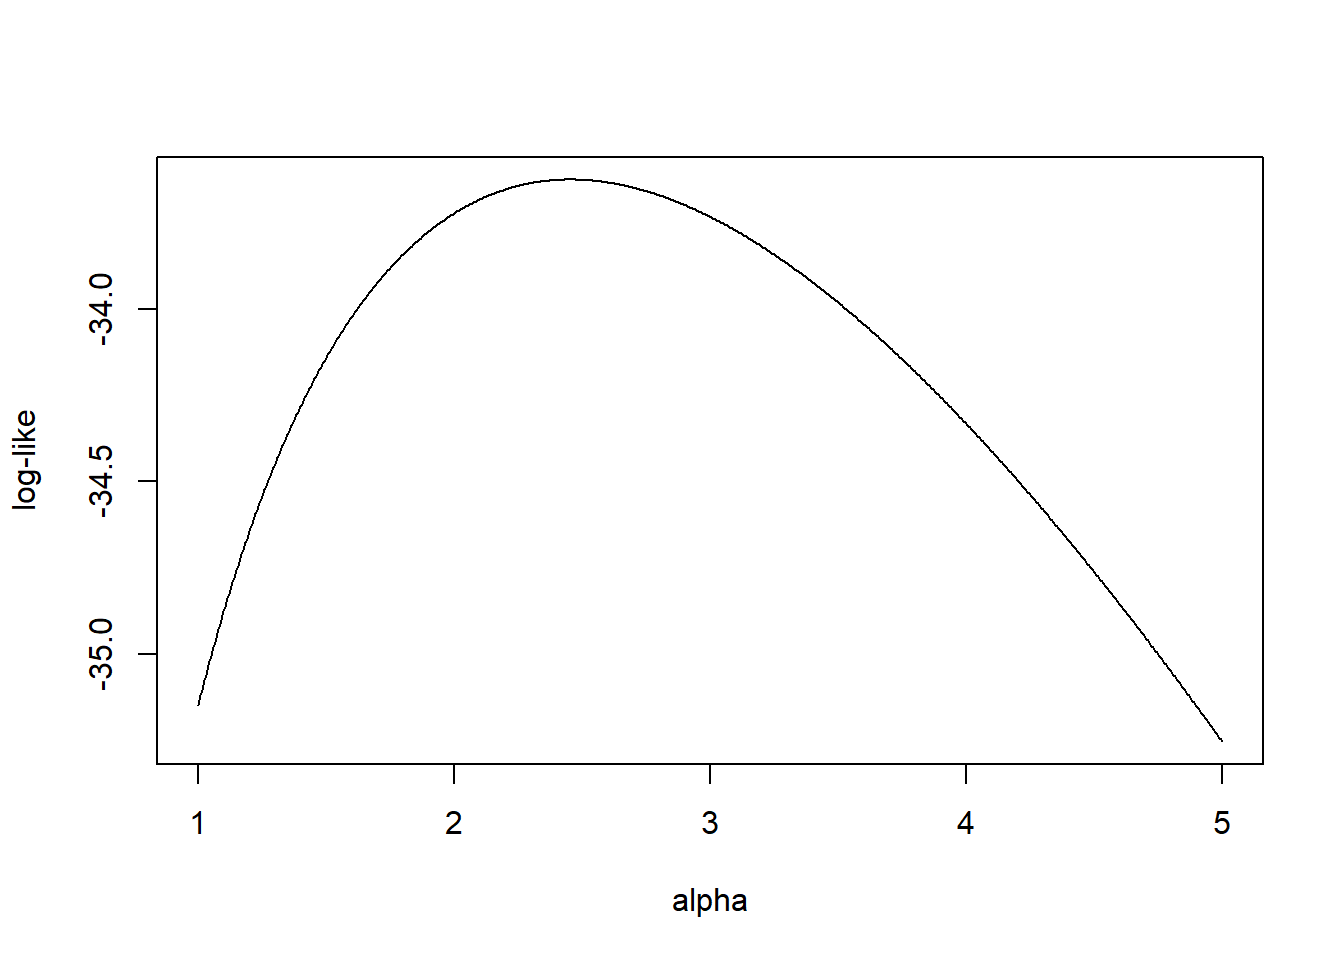
\includegraphics{LossDataAnalytics_files/figure-latex/LoglikeOnePareto-1} 

}

\caption{Verosimilitud logarítmica para una Pareto de un parámetro}\label{fig:LoglikeOnePareto}
\end{figure}

Se puede determinar el valor máximo del logaritmo de la verosimilitud tomando derivadas e igualándolas a cero.
De esto resulta
\[
\frac{ \partial}{\partial \alpha } l(\alpha |\mathbf{x}) =    5  \ln 500 + 5 / \alpha -  \sum_{i=1}^5 \ln x_i
=_{set} 0 \Rightarrow \hat{\alpha}_{MLE} = \frac{5}{\sum_{i=1}^5 \ln x_i - 5  \ln 500 } = 2,453 .
\]

Naturalmente, hay muchos problemas en los que no es práctico realizar un cálculo manual para la optimización. Afortunadamente hay muchas rutinas estadísticas disponibles como la función \texttt{optim} de \texttt{R}.

\begin{Shaded}
\begin{Highlighting}[]
\NormalTok{c1 }\OtherTok{\textless{}{-}} \FunctionTok{log}\NormalTok{(}\DecValTok{521}\NormalTok{)}\SpecialCharTok{+}\FunctionTok{log}\NormalTok{(}\DecValTok{658}\NormalTok{)}\SpecialCharTok{+}\FunctionTok{log}\NormalTok{(}\DecValTok{702}\NormalTok{)}\SpecialCharTok{+}\FunctionTok{log}\NormalTok{(}\DecValTok{819}\NormalTok{)}\SpecialCharTok{+}\FunctionTok{log}\NormalTok{(}\DecValTok{1217}\NormalTok{)}
\NormalTok{nloglike }\OtherTok{\textless{}{-}} \ControlFlowTok{function}\NormalTok{(alpha)\{}\SpecialCharTok{{-}}\NormalTok{(}\DecValTok{5}\SpecialCharTok{*}\NormalTok{alpha}\SpecialCharTok{*}\FunctionTok{log}\NormalTok{(}\DecValTok{500}\NormalTok{)}\SpecialCharTok{+}\DecValTok{5}\SpecialCharTok{*}\FunctionTok{log}\NormalTok{(alpha)}\SpecialCharTok{{-}}\NormalTok{(alpha}\SpecialCharTok{+}\DecValTok{1}\NormalTok{)}\SpecialCharTok{*}\NormalTok{c1)\}}
\NormalTok{MLE }\OtherTok{\textless{}{-}} \FunctionTok{optim}\NormalTok{(}\AttributeTok{par=}\DecValTok{1}\NormalTok{, }\AttributeTok{fn=}\NormalTok{nloglike)}\SpecialCharTok{$}\NormalTok{par}
\end{Highlighting}
\end{Shaded}

\begin{center}\rule{0.5\linewidth}{0.5pt}\end{center}

Este código confirma el resultado del cálculo manual en el que el estimador máximo verosímil es \(\alpha_{MLE} =\) 2.453125.

\begin{center}\rule{0.5\linewidth}{0.5pt}\end{center}

Se presentan algunos ejemplos adicionales para ilustrar cómo los actuarios ajustan modelos de distribución paramétricos a una base de datos de siniestros usando máxima verosimilitud.

\textbf{Ejemmplo 3.5.2. Pregunta de examen actuarial.}
Se considera una muestra aleatoria de cuantías de siniestros: 8.000 10.000 12.000 15.000. Se asume que la cuantía de los siniestros sigue una distribución inversa exponencial, con parámetro \(\theta\). Calcula el estimador máximo verosímil de \(\theta\).

\textbf{Solución.}

La función de densidad de probabilidad es
\[f_{X}\left( x \right) = \frac{\theta e^{- \frac{\theta}{x}}}{x^{2}}, \]
donde \(x > 0\).

La función de verosimilitud, \(L\left( \theta \right)\), puede ser vista como la probabilidad de los datos observados, expresada en función de los parámetros del modelo
\(\theta\)
\[L\left( \theta \right) = \prod_{i = 1}^{4}{f_{X_{i}}\left( x_{i} \right)} = \frac{\theta^{4}e^{- \theta\sum_{i = 1}^{4}\frac{1}{x_{i}}}}{\prod_{i = 1}^{4}x_{i}^{2}}.\]

El logaritmo de la función de verosimilitud, \(\ln L \left( \theta \right)\), es la suma de los logarítmos individuales.
\[\ln L \left( \theta \right) = 4 \ln \theta - \theta\sum_{i = 1}^{4}\frac{1}{x_{i}} - 2\sum_{i = 1}^{4}\ln x_{i} .\]

\[
\frac{d \ln L \left( \theta \right)}{d \theta} = \frac{4}{\theta} - \sum_{i = 1}^{4}\frac{1}{x_{i}}.
\]

El estimador máximo verosímil de \(\theta\), denotado como \(\hat{\theta}\), es la solución para la ecuación
\[\frac{4}{\hat{\theta}} - \sum_{i = 1}^{4}{\frac{1}{x_{i}} = 0}.\] Por tanto,
\(\hat{\theta} = \frac{4}{\sum_{i = 1}^{4}\frac{1}{x_{i}}} = 10.667\)

La segunda derivada de \(\ln L \left( \theta \right)\) viene dada por
\[\frac{d^{2}\ln L\left( \theta \right)}{d\theta^{2}} = \frac{- 4}{\theta^{2}}.\]
Evaluando la segunda derivada del logaritmo de la función de verosimilitud en \(\hat{\theta} = 10.667\) da un valor negativo, lo cual indica que \(\hat{\theta}\) es el valor que maximiza el logaritmo de la función de verosimilitud.

\begin{center}\rule{0.5\linewidth}{0.5pt}\end{center}

\textbf{Ejemplo 3.5.3. Pregunta del examen actuarial.}
Una muestra aleatoria de tamaño 6 proviene de una distribución lognormal con parámetros \(\mu\) y \(\sigma\). Los valores de la muestra son 200, 3.000, 8.000, 60.000, 60.000, 160.000. Calcula el estimador máximo verosímil de \(\mu\) y \(\sigma\).

\textbf{Solución.}

La función de densidad de probabilidad es
\[f_{X}\left( x \right) = \frac{1}{x \sigma \sqrt{2\pi}}\exp - \frac{1}{2}\left( \frac{\ln x - \mu}{\sigma} \right)^{2},\]
donde \(x > 0\).

La función de verosimilitud, \(L\left( \mu,\sigma \right)\), es el producto de la \emph{pdf} para cada punto.
\[L\left( \mu,\sigma \right) = \prod_{i = 1}^{6}{f_{X_{i}}\left( x_{i} \right)} = \frac{1}{\sigma^{6}\left( 2\pi \right)^{3}\prod_{i = 1}^{6}x_{i}}exp - \frac{1}{2}\sum_{i = 1}^{6}\left( \frac{\ln x_{i} - \mu}{\sigma} \right)^{2}.\]
El logaritmo de la función de verosimilitud, \(\ln L \left( \mu,\sigma \right)\), es la suma de los logaritmos individuales.
\[\ln \left( \mu,\sigma \right) = - 6 \ln \sigma - 3 \ln \left( 2\pi \right) - \sum_{i = 1}^{6}\ln x_{i} - \frac{1}{2}\sum_{i = 1}^{6}\left( \frac{\ln x_{i} - \mu}{\sigma} \right)^{2}.\]
Las primeras derivadas parciales son
\[\frac{\partial \ln L\left( \mu,\sigma \right)}{\partial\mu} = \frac{1}{\sigma^{2}}\sum_{i = 1}^{6}\left( \ln x_{i} - \mu \right).\]
\[\frac{\partial \ln L\left( \mu,\sigma \right)}{\partial\sigma} = \frac{- 6}{\sigma} + \frac{1}{\sigma^{3}}\sum_{i = 1}^{6}\left( \ln x_{i} - \mu \right)^{2}.\]
Los estimadores máximo verosímiles de \(\mu\) y \(\sigma\), denotados como \(\hat{\mu}\) y \(\hat{\sigma}\), son las soluciones de las ecuaciones
\[\frac{1}{{\hat{\sigma}}^{2}}\sum_{i = 1}^{6}\left( \ln x_{i} - \hat{\mu} \right) = 0.\]
\[\frac{- 6}{\hat{\sigma}} + \frac{1}{{\hat{\sigma}}^{3}}\sum_{i = 1}^{6}\left( \ln x_{i} - \hat{\mu} \right)^{2} = 0.\]
Esto resulta en las estimaciones

\[\hat{\mu} = \frac{\sum_{i = 1}^{6}{\ln x_{i}}}{6} = 9,38 \ \ \ \text{y} \ \ \ 
{\hat{\sigma}}^{2} = \frac{\sum_{i = 1}^{6}\left( \ln x_{i} - \hat{\mu} \right)^{2}}{6} = 5,12 .
\].

Las segundas derivadas parciales son

\[
\frac{\partial^{2}\ln L\left( \mu,\sigma \right)}{\partial\mu^{2}} = \frac{- 6}{\sigma^{2}}, \ \ \ \ 
\frac{\partial^{2}\ln L\left( \mu,\sigma \right)}{\partial\mu\partial\sigma} = \frac{- 2}{\sigma^{3}}\sum_{i = 1}^{6}\left( \ln x_{i} - \mu \right)
\]

y

\[
\frac{\partial^{2}\ln L\left( \mu,\sigma \right)}{\partial\sigma^{2}} = \frac{6}{\sigma^{2}} - \frac{3}{\sigma^{4}}\sum_{i = 1}^{6}\left( \ln x_{i} - \mu \right)^{2}
\].

\begin{center}\rule{0.5\linewidth}{0.5pt}\end{center}

Dos cuestiones que vendrían a continuación tienen que ver con las propiedades para muestras grandes que el lector puede haber visto en cursos anteriores. El Capítulo del Apéndice \ref{C:AppC} revisa la definición de función de verosimilitud, introduce sus propiedades, revisa los estimadores máximo verosímiles, extiende sus propiedades para muestras grandes al caso en el que hay múltiples parámetros en el modelo, y revisa la inferencia estadística basada en los estimadores máximo verosímiles. En las soluciones de estos ejemplos se derivan las varianzas asintóticas de los estimadores máximo verosímiles de los parámetros del modelo. Se usa el método delta para derivar las varianzas asintóticas de las funciones de estos parámetros.

\textbf{Ejemplo 3.5.2 - Continuación.} Se refiere al \textbf{Ejemplo 3.5.2.}

Aproxima la varianza del estimador máximo verosímil.

Determina un intervalo de confianza para \(\theta\) al 95\%.

Determina un intervalo de confianza del 95\% para \(\Pr \left( X \leq 9.000 \right).\)

\textbf{Solución.}

\textbf{a.} Tomando el recíproco de la esperanza negativa de la segunda derivada de \(\ln L \left( \theta \right)\), se obtiene una estimación de la varianza de \(\hat{\theta}\),
\(\widehat{Var}\left( \hat{\theta} \right) = \left. \ \left\lbrack E\left( \frac{d^{2}\ln L \left( \theta \right)}{d\theta^{2}} \right) \right\rbrack^{- 1} \right|_{\theta = \hat{\theta}} = \frac{{\hat{\theta}}^{2}}{4} = 28.446.222\).

Nótese que dado que el tamaño de la muestra \(n \rightarrow \infty\), la distribución del estimador máximo verosímil \(\hat{\theta}\) converge a una distribución normal con media \(\theta\) y varianza \(\hat{V}\left( \hat{\theta} \right)\). El intervalo de confianza aproximado en este ejemplo se basa en el supuesto de normalidad, a pesar del pequeño tamaño muestral, solo con fines ilustrativos.

\textbf{b.} El intervalo de confianza al 95\% para \(\theta\) viene dado por

\[
10.667 \pm 1,96\sqrt{28.446.222} = \left( 213,34,\ 21.120,66 \right).
\]

\textbf{c.} La función de distribución de \(X\) es \(F\left( x \right) = 1 - e^{- \frac{x}{\theta}}\). Entonces, el estimador máximo verosímil de \(g_{\Theta}(\theta) = F\left( 9.000 \right)\) es
\[g\left( \hat{\theta} \right) = 1 - e^{- \frac{9.000}{10.667}} = 0,57.\]
Se usa el método delta para aproximar la varianza de \(g\left( \hat{\theta} \right)\).
\[\frac{\text{dg}\left( \theta \right)}{d \theta} = {- \frac{9.000}{\theta^{2}}e}^{- \frac{9.000}{\theta}}.\]

\(\widehat{Var}\left\lbrack g\left( \hat{\theta} \right) \right\rbrack = \left( - {\frac{9.000}{{\hat{\theta}}^{2}}e}^{- \frac{9.000}{\hat{\theta}}} \right)^{2}\hat{V}\left( \hat{\theta} \right) = 0,0329\).

El intervalo de confianza al 95\% para \(F\left( 9.000 \right)\) viene dado por
\[0,57 \pm 1,96\sqrt{0,0329} = \left( 0,214,\ 0,926 \right).\]

\begin{center}\rule{0.5\linewidth}{0.5pt}\end{center}

\textbf{Ejemplo 3.5.3 - Continuación.} Se refiere al \textbf{Ejemplo 3.5.3.}

Estima la matriz de covarianzas del estimador máximo verosímil.

Determina intervalos de confianza aproximados al 95\% para \(\mu\) y \(\sigma\).

Determina un intervalo de confianza aproximado al 95\% para la media de la distribución lognormal.

\textbf{a.} Para obtener la matriz de covarianzas del \emph{mle} es necesario encontrar esperanzas de las segundas derivadas. Dado que la variable aleatoria \(X\) sigue una distribución lognormal con parámetros \(\mu\) y \(\sigma\), entonces \(\text{lnX}\) se distribuye como una normal con media \(\mu\) y varianza \(\sigma^{2}\).

\(\mathrm{E}\left( \frac{\partial^{2}\text{lnL}\left( \mu,\sigma \right)}{\partial\mu^{2}} \right) = \mathrm{E}\left( \frac{- 6}{\sigma^{2}} \right) = \frac{- 6}{\sigma^{2}}\),

\(\mathrm{E}\left( \frac{\partial^{2}\text{lnL}\left( \mu,\sigma \right)}{\partial\mu\partial\sigma} \right) = \frac{- 2}{\sigma^{3}}\sum_{i = 1}^{6}{\mathrm{E}\left( \ln x_{i} - \mu \right)} = \frac{- 2}{\sigma^{3}}\sum_{i = 1}^{6}\left\lbrack \mathrm{E}\left( \ln x_{i} \right) - \mu \right\rbrack\)=\(\frac{- 2}{\sigma^{3}}\sum_{i = 1}^{6}\left( \mu - \mu \right) = 0\),

y

\(\mathrm{E}\left( \frac{\partial^{2}\text{lnL}\left( \mu,\sigma \right)}{\partial\sigma^{2}} \right) = \frac{6}{\sigma^{2}} - \frac{3}{\sigma^{4}}\sum_{i = 1}^{6}{\mathrm{E}\left( \ln x_{i} - \mu \right)}^{2} = \frac{6}{\sigma^{2}} - \frac{3}{\sigma^{4}}\sum_{i = 1}^{6}{\mathrm{V}\left( \ln x_{i} \right) = \frac{6}{\sigma^{2}} - \frac{3}{\sigma^{4}}\sum_{i = 1}^{6}{\sigma^{2} = \frac{- 12}{\sigma^{2}}}}\).

Usando el negativo de estas esperanzas se obtiene la matriz de información de Fisher \[\begin{bmatrix}
\frac{6}{\sigma^{2}} & 0 \\
0 & \frac{12}{\sigma^{2}} \\
\end{bmatrix}.\]

La matriz de covarianzas, \(\Sigma\), es la inversa de la matriz de información de Fisher \[\Sigma = \begin{bmatrix}
\frac{\sigma^{2}}{6} & 0 \\
0 & \frac{\sigma^{2}}{12} \\
\end{bmatrix}.\]

La matriz estimada viene dada por \[\hat{\Sigma} = \begin{bmatrix}
0,8533 & 0 \\
0 & 0,4267 \\
\end{bmatrix}.\]

\textbf{b.} El intervalo de confianza al 95\% para \(\mu\) viene dado por \(9,38 \pm 1,96\sqrt{0,8533} = \left( 7,57,\ 11,19 \right)\).

El intervalo de confianza al 95\% para \(\sigma^{2}\) viene dado por \(5,12 \pm 1,96\sqrt{0,4267} = \left( 3,84,\ 6,40 \right)\).

\textbf{c.} La media de \emph{X} es \(\exp\left( \mu + \frac{\sigma^{2}}{2} \right)\). Entonces, el estimador máximo verosímil de
\[g\left( \mu,\sigma \right) = \exp\left( \mu + \frac{\sigma^{2}}{2} \right)\]
es
\[g\left( \hat{\mu},\hat{\sigma} \right) = \exp\left( \hat{\mu} + \frac{{\hat{\sigma}}^{2}}{2} \right) = 153.277.\]

Se usa el método delta para aproximar la varianza del mle
\(g\left( \hat{\mu},\hat{\sigma} \right)\).

\(\frac{\partial g\left( \mu,\sigma \right)}{\partial\mu} = exp\left( \mu + \frac{\sigma^{2}}{2} \right)\)
y
\(\frac{\partial g\left( \mu,\sigma \right)}{\partial\sigma} = \sigma exp\left( \mu + \frac{\sigma^{2}}{2} \right)\).

Usando el método delta, la varianza aproximada de
\(g\left( \hat{\mu},\hat{\sigma} \right)\) viene dada por

\[\left. \ \hat{V}\left( g\left( \hat{\mu},\hat{\sigma} \right) \right) = \begin{bmatrix}
\frac{\partial g\left( \mu,\sigma \right)}{\partial\mu} & \frac{\partial g\left( \mu,\sigma \right)}{\partial\sigma} \\
\end{bmatrix}\Sigma\begin{bmatrix}
\frac{\partial g\left( \mu,\sigma \right)}{\partial\mu} \\
\frac{\partial g\left( \mu,\sigma \right)}{\partial\sigma} \\
\end{bmatrix} \right|_{\mu = \hat{\mu},\sigma = \hat{\sigma}}\]

\[= \begin{bmatrix}
153.277 & 346.826 \\
\end{bmatrix}\begin{bmatrix}
0,8533 & 0 \\
0 & 0,4267 \\
\end{bmatrix}\begin{bmatrix}
153.277 \\
346.826 \\
\end{bmatrix} =\]71.374.380.000

El intervalo de confianza al 95\% para \(\exp\left( \mu + \frac{\sigma^{2}}{2} \right)\) viene dado por

\(153.277 \pm 1,96\sqrt{71.374.380.000} = \left( - 370.356,\ 676.910 \right)\).

Dado que la media de la distribución lognormal no puede ser negativa, se debería reemplazar el límite inferior negativo en el intervalo anterior por cero.

\begin{center}\rule{0.5\linewidth}{0.5pt}\end{center}

\textbf{Ejemplo 3.5.4. Fondo de propiedad de Wisconsin.} Para ver cómo los estimadores máximo verosímiles se aplican a datos reales, volvemos a los 2010 datos de siniestros introducidos en la Sección \ref{S:LGPIF}.

El siguiente fragmento de código muestra cómo ajustar un modelo exponencial, gamma, Pareto, lognormal y GB2. Por consistencia, el código emplea el paquete \texttt{VGAM} de \texttt{R}. El acrónimo viene de \emph{Vector Generalized Linear and Additive Models}; como sugiere el nombre, este paquete puede hacer mucho más que ajustar estos modelos, aunque esto es suficiente para los propósitos requeridos en este caso. La única excepción es la densidad GB2 que no es muy utilizada fuera del mundo asegurador; en cualquier caso, puede programarse esta densidad y calcular los estimadores máximo verosímiles usando el optimizador general \texttt{optim}.

\begin{Shaded}
\begin{Highlighting}[]
\FunctionTok{library}\NormalTok{(VGAM)}
\NormalTok{claim\_lev }\OtherTok{\textless{}{-}} \FunctionTok{read.csv}\NormalTok{(}\StringTok{"Data/CLAIMLEVEL.csv"}\NormalTok{, }\AttributeTok{header =} \ConstantTok{TRUE}\NormalTok{) }
\NormalTok{claim\_data }\OtherTok{\textless{}{-}} \FunctionTok{subset}\NormalTok{(claim\_lev, Year }\SpecialCharTok{==} \DecValTok{2010}\NormalTok{); }

\CommentTok{\# Inferencia usando una distribución GB2 – más complicado}
\CommentTok{\# La función de verosimilitud de una distribución GB2 (negativo para optimización)}
\NormalTok{lik\_gb2 }\OtherTok{\textless{}{-}} \ControlFlowTok{function}\NormalTok{ (param) \{}
\NormalTok{  a\_1 }\OtherTok{\textless{}{-}}\NormalTok{ param[}\DecValTok{1}\NormalTok{]}
\NormalTok{  a\_2 }\OtherTok{\textless{}{-}}\NormalTok{ param[}\DecValTok{2}\NormalTok{]}
\NormalTok{  mu }\OtherTok{\textless{}{-}}\NormalTok{ param[}\DecValTok{3}\NormalTok{]}
\NormalTok{  sigma }\OtherTok{\textless{}{-}}\NormalTok{ param[}\DecValTok{4}\NormalTok{]}
\NormalTok{  yt }\OtherTok{\textless{}{-}}\NormalTok{ (}\FunctionTok{log}\NormalTok{(claim\_data}\SpecialCharTok{$}\NormalTok{Claim) }\SpecialCharTok{{-}}\NormalTok{ mu) }\SpecialCharTok{/}\NormalTok{ sigma}
\NormalTok{  logexpyt }\OtherTok{\textless{}{-}} \FunctionTok{ifelse}\NormalTok{(yt }\SpecialCharTok{\textgreater{}} \DecValTok{23}\NormalTok{, yt, }\FunctionTok{log}\NormalTok{(}\DecValTok{1} \SpecialCharTok{+} \FunctionTok{exp}\NormalTok{(yt)))}
\NormalTok{  logdens }\OtherTok{\textless{}{-}}\NormalTok{ a\_1 }\SpecialCharTok{*}\NormalTok{ yt }\SpecialCharTok{{-}} \FunctionTok{log}\NormalTok{(sigma) }\SpecialCharTok{{-}} \FunctionTok{log}\NormalTok{(}\FunctionTok{beta}\NormalTok{(a\_1,a\_2)) }\SpecialCharTok{{-}} 
\NormalTok{    (a\_1}\SpecialCharTok{+}\NormalTok{a\_2) }\SpecialCharTok{*}\NormalTok{ logexpyt }\SpecialCharTok{{-}} \FunctionTok{log}\NormalTok{(claim\_data}\SpecialCharTok{$}\NormalTok{Claim) }
  \FunctionTok{return}\NormalTok{(}\SpecialCharTok{{-}}\FunctionTok{sum}\NormalTok{(logdens))}
\NormalTok{\}}
\CommentTok{\# "optim" es una función general utilizada con propósito de minimizar}
\NormalTok{gb2\_bop }\OtherTok{\textless{}{-}} \FunctionTok{optim}\NormalTok{(}\FunctionTok{c}\NormalTok{(}\DecValTok{1}\NormalTok{, }\DecValTok{1}\NormalTok{, }\DecValTok{0}\NormalTok{, }\DecValTok{1}\NormalTok{), lik\_gb2, }\AttributeTok{method =} \FunctionTok{c}\NormalTok{(}\StringTok{"L{-}BFGS{-}B"}\NormalTok{), }
                 \AttributeTok{lower =} \FunctionTok{c}\NormalTok{(}\FloatTok{0.01}\NormalTok{, }\FloatTok{0.01}\NormalTok{, }\SpecialCharTok{{-}}\DecValTok{500}\NormalTok{, }\FloatTok{0.01}\NormalTok{), }
                 \AttributeTok{upper =} \FunctionTok{c}\NormalTok{(}\DecValTok{500}\NormalTok{, }\DecValTok{500}\NormalTok{, }\DecValTok{500}\NormalTok{, }\DecValTok{500}\NormalTok{), }\AttributeTok{hessian =} \ConstantTok{TRUE}\NormalTok{)}
\CommentTok{\# Gráfico no paramétrico}
\FunctionTok{plot}\NormalTok{(}\FunctionTok{density}\NormalTok{(}\FunctionTok{log}\NormalTok{(claim\_data}\SpecialCharTok{$}\NormalTok{Claim)), }\AttributeTok{main =} \StringTok{""}\NormalTok{, }\AttributeTok{xlab =} \StringTok{"Gastos logarítmicos"}\NormalTok{,}
     \AttributeTok{ylim =} \FunctionTok{c}\NormalTok{(}\DecValTok{0}\NormalTok{ ,}\FloatTok{0.37}\NormalTok{))}
\NormalTok{x }\OtherTok{\textless{}{-}} \FunctionTok{seq}\NormalTok{(}\DecValTok{0}\NormalTok{, }\DecValTok{15}\NormalTok{, }\AttributeTok{by =} \FloatTok{0.01}\NormalTok{)}
\CommentTok{\#Exponencial}
\NormalTok{fit.exp }\OtherTok{\textless{}{-}} \FunctionTok{vglm}\NormalTok{(Claim }\SpecialCharTok{\textasciitilde{}} \DecValTok{1}\NormalTok{, exponential, }\AttributeTok{data =}\NormalTok{ claim\_data)}
\NormalTok{theta }\OtherTok{=} \DecValTok{1} \SpecialCharTok{/} \FunctionTok{exp}\NormalTok{(}\FunctionTok{coef}\NormalTok{(fit.exp))}
\NormalTok{fexp\_ex }\OtherTok{\textless{}{-}} \FunctionTok{dgamma}\NormalTok{(}\FunctionTok{exp}\NormalTok{(x), }\AttributeTok{scale =} \FunctionTok{exp}\NormalTok{(}\SpecialCharTok{{-}}\FunctionTok{coef}\NormalTok{(fit.exp)), }\AttributeTok{shape =} \DecValTok{1}\NormalTok{) }\SpecialCharTok{*} \FunctionTok{exp}\NormalTok{(x)}
\FunctionTok{lines}\NormalTok{(x, fexp\_ex, }\AttributeTok{col =} \StringTok{"red"}\NormalTok{, }\AttributeTok{lty =}\DecValTok{2}\NormalTok{)}
\CommentTok{\# Inferencia asumiendo una distribución gamma}
\NormalTok{fit.gamma }\OtherTok{\textless{}{-}} \FunctionTok{vglm}\NormalTok{(Claim }\SpecialCharTok{\textasciitilde{}} \DecValTok{1}\NormalTok{, }\AttributeTok{family =}\NormalTok{ gamma2, }\AttributeTok{data =}\NormalTok{ claim\_data)}
\NormalTok{theta }\OtherTok{\textless{}{-}} \FunctionTok{exp}\NormalTok{(}\FunctionTok{coef}\NormalTok{(fit.gamma)[}\DecValTok{1}\NormalTok{]) }\SpecialCharTok{/} \FunctionTok{exp}\NormalTok{(}\FunctionTok{coef}\NormalTok{(fit.gamma)[}\DecValTok{2}\NormalTok{])  }\CommentTok{\# theta = mu / alpha}
\NormalTok{alpha }\OtherTok{\textless{}{-}} \FunctionTok{exp}\NormalTok{(}\FunctionTok{coef}\NormalTok{(fit.gamma)[}\DecValTok{2}\NormalTok{]) }
\NormalTok{fgamma\_ex }\OtherTok{\textless{}{-}} \FunctionTok{dgamma}\NormalTok{(}\FunctionTok{exp}\NormalTok{(x), }\AttributeTok{shape =}\NormalTok{ alpha, }\AttributeTok{scale =}\NormalTok{ theta) }\SpecialCharTok{*} \FunctionTok{exp}\NormalTok{(x)}
\FunctionTok{lines}\NormalTok{(x, fgamma\_ex, }\AttributeTok{col =} \StringTok{"blue"}\NormalTok{, }\AttributeTok{lty =}\DecValTok{3}\NormalTok{)}
\CommentTok{\#Pareto}
\NormalTok{fit.pareto }\OtherTok{\textless{}{-}} \FunctionTok{vglm}\NormalTok{(Claim }\SpecialCharTok{\textasciitilde{}} \DecValTok{1}\NormalTok{, paretoII, }\AttributeTok{loc =} \DecValTok{0}\NormalTok{, }\AttributeTok{data =}\NormalTok{ claim\_data)}
\NormalTok{fpareto\_ex }\OtherTok{\textless{}{-}} \FunctionTok{dparetoII}\NormalTok{(}\FunctionTok{exp}\NormalTok{(x), }\AttributeTok{loc =} \DecValTok{0}\NormalTok{, }\AttributeTok{shape =} \FunctionTok{exp}\NormalTok{(}\FunctionTok{coef}\NormalTok{(fit.pareto)[}\DecValTok{2}\NormalTok{]), }
                        \AttributeTok{scale =} \FunctionTok{exp}\NormalTok{(}\FunctionTok{coef}\NormalTok{(fit.pareto)[}\DecValTok{1}\NormalTok{])) }\SpecialCharTok{*} \FunctionTok{exp}\NormalTok{(x)}
\FunctionTok{lines}\NormalTok{(x, fpareto\_ex, }\AttributeTok{col =} \StringTok{"purple"}\NormalTok{)}
\CommentTok{\# Lognormal}
\NormalTok{fit.LN }\OtherTok{\textless{}{-}} \FunctionTok{vglm}\NormalTok{(Claim }\SpecialCharTok{\textasciitilde{}} \DecValTok{1}\NormalTok{, }\AttributeTok{family =}\NormalTok{ lognormal, }\AttributeTok{data =}\NormalTok{ claim\_data)}
\NormalTok{flnorm\_ex }\OtherTok{\textless{}{-}} \FunctionTok{dlnorm}\NormalTok{(}\FunctionTok{exp}\NormalTok{(x), }\AttributeTok{mean =} \FunctionTok{coef}\NormalTok{(fit.LN)[}\DecValTok{1}\NormalTok{],}
                    \AttributeTok{sd =} \FunctionTok{exp}\NormalTok{(}\FunctionTok{coef}\NormalTok{(fit.LN)[}\DecValTok{2}\NormalTok{])) }\SpecialCharTok{*} \FunctionTok{exp}\NormalTok{(x)}
\FunctionTok{lines}\NormalTok{(x, flnorm\_ex, }\AttributeTok{col =} \StringTok{"lightblue"}\NormalTok{)}
\CommentTok{\# Densidad para GB II}
\NormalTok{gb2\_density }\OtherTok{\textless{}{-}} \ControlFlowTok{function}\NormalTok{ (x) \{}
\NormalTok{  a\_1 }\OtherTok{\textless{}{-}}\NormalTok{ gb2\_bop}\SpecialCharTok{$}\NormalTok{par[}\DecValTok{1}\NormalTok{]}
\NormalTok{  a\_2 }\OtherTok{\textless{}{-}}\NormalTok{ gb2\_bop}\SpecialCharTok{$}\NormalTok{par[}\DecValTok{2}\NormalTok{]}
\NormalTok{  mu }\OtherTok{\textless{}{-}}\NormalTok{ gb2\_bop}\SpecialCharTok{$}\NormalTok{par[}\DecValTok{3}\NormalTok{]}
\NormalTok{  sigma }\OtherTok{\textless{}{-}}\NormalTok{ gb2\_bop}\SpecialCharTok{$}\NormalTok{par[}\DecValTok{4}\NormalTok{]}
\NormalTok{  xt }\OtherTok{\textless{}{-}}\NormalTok{ (}\FunctionTok{log}\NormalTok{(x) }\SpecialCharTok{{-}}\NormalTok{ mu) }\SpecialCharTok{/}\NormalTok{ sigma}
\NormalTok{  logexpxt }\OtherTok{\textless{}{-}} \FunctionTok{ifelse}\NormalTok{ (xt }\SpecialCharTok{\textgreater{}} \DecValTok{23}\NormalTok{, yt, }\FunctionTok{log}\NormalTok{(}\DecValTok{1} \SpecialCharTok{+} \FunctionTok{exp}\NormalTok{(xt)))}
\NormalTok{  logdens }\OtherTok{\textless{}{-}}\NormalTok{ a\_1 }\SpecialCharTok{*}\NormalTok{ xt }\SpecialCharTok{{-}} \FunctionTok{log}\NormalTok{(sigma) }\SpecialCharTok{{-}} \FunctionTok{log}\NormalTok{(}\FunctionTok{beta}\NormalTok{(a\_1, a\_2)) }\SpecialCharTok{{-}} 
\NormalTok{    (a\_1}\SpecialCharTok{+}\NormalTok{a\_2) }\SpecialCharTok{*}\NormalTok{ logexpxt }\SpecialCharTok{{-}}\FunctionTok{log}\NormalTok{(x) }
  \FunctionTok{exp}\NormalTok{(logdens)}
\NormalTok{  \}}
\NormalTok{fGB2\_ex }\OtherTok{=} \FunctionTok{gb2\_density}\NormalTok{(}\FunctionTok{exp}\NormalTok{(x)) }\SpecialCharTok{*} \FunctionTok{exp}\NormalTok{(x)}
\FunctionTok{lines}\NormalTok{(x, fGB2\_ex, }\AttributeTok{col=}\StringTok{"green"}\NormalTok{)}
\FunctionTok{legend}\NormalTok{(}\StringTok{"topleft"}\NormalTok{, }\FunctionTok{c}\NormalTok{(}\StringTok{"log(Gastos)"}\NormalTok{, }\StringTok{"Exponencial"}\NormalTok{, }\StringTok{"Gamma"}\NormalTok{, }\StringTok{"Pareto"}\NormalTok{, }
                    \StringTok{"Lognormal"}\NormalTok{, }\StringTok{"GB2"}\NormalTok{), }\AttributeTok{cex=}\FloatTok{0.8}\NormalTok{,}
       \AttributeTok{lty =} \FunctionTok{c}\NormalTok{(}\DecValTok{4}\NormalTok{,}\DecValTok{2}\NormalTok{,}\DecValTok{3}\NormalTok{,}\DecValTok{1}\NormalTok{,}\DecValTok{1}\NormalTok{,}\DecValTok{1}\NormalTok{), }\CommentTok{\#4 is "longdash"}
       \AttributeTok{col =} \FunctionTok{c}\NormalTok{(}\StringTok{"black"}\NormalTok{,}\StringTok{"red"}\NormalTok{,}\StringTok{"blue"}\NormalTok{,}\StringTok{"purple"}\NormalTok{,}\StringTok{"lightblue"}\NormalTok{,}\StringTok{"green"}\NormalTok{))}
\end{Highlighting}
\end{Shaded}

\begin{figure}

{\centering 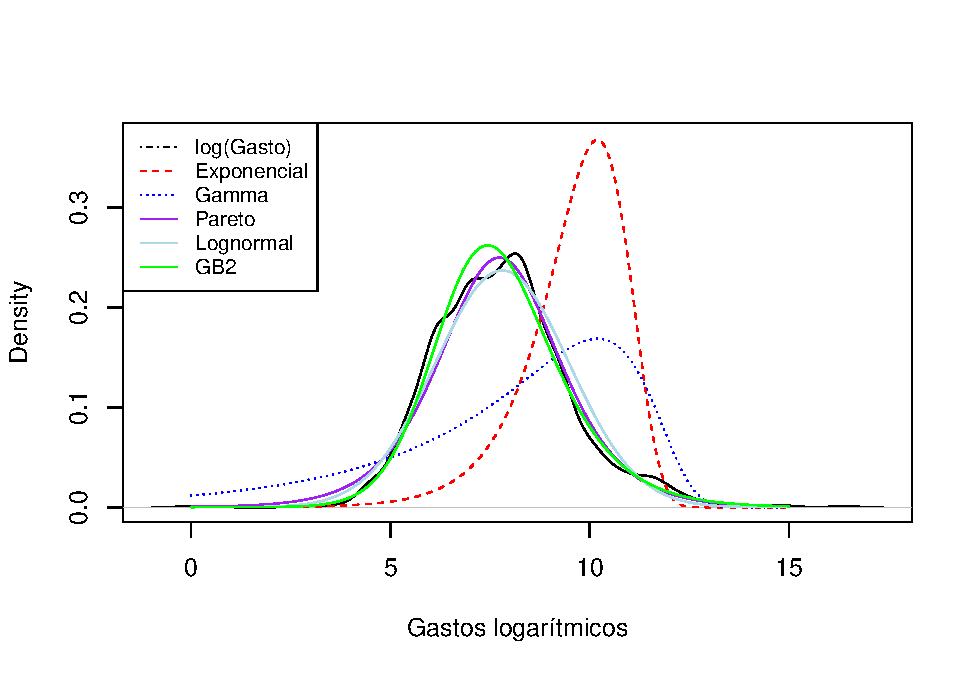
\includegraphics{LossDataAnalytics_files/figure-latex/MLECompare-1} 

}

\caption{Comparaciones de densidad para el fondo de propiedad de Wisconsin}\label{fig:MLECompare}
\end{figure}

Los resultados del ejercicio de ajuste se resumen en la Figura \ref{fig:MLECompare}. Aquí, la curva negra de rayas largas es un histograma suavizado para los datos reales (que introduciremos en la Sección \ref{S:MS:NonParInf}); las otras curvas son curvas paramétricas donde los parámetros se calculan vía máxima verosimilitud. Se aprecia un pobre ajuste en la línia de rayas rojas correspondiente al ajuste de la distribución exponencial y la línea de puntos azules correspondiente al ajuste de la distribución gamma. Los ajustes de las otras curvas, Pareto, lognormal y GB2, parecen proporcionar un ajuste razonablemente bueno a los datos reales. En el Capítulo \ref{C:ModelSelection} se describe en más detalle los principios para la selección de modelos.

\begin{center}\rule{0.5\linewidth}{0.5pt}\end{center}

\hypertarget{S:Loss:MLEModified}{%
\subsection{Estimadores por máxima verosimilitud usando datos modificados}\label{S:Loss:MLEModified}}

En muchas aplicaciones, los actuarios y otros analistas desean estimar modelos paramétricos basados en datos individuales que no están limitados. En cualquier caso, hay también importantes aplicaciones en las que solo hay datos disponibles que están limitados o \emph{modificados}. Esta sección introduce la estimación máximo verosímil para datos agrupados, censurados y truncados. Más adelante, se continuará con detalles adicionales en la Sección \ref{S:MS:ModifiedData}.

\hypertarget{MLEGrouped}{%
\subsubsection{Estimadores por máxima verosimilitud para datos agrupados}\label{MLEGrouped}}

En la sección anterior se consideró la estimación máximo verosímil de modelos continuos a partir de datos (individuales) completos. Cada observación individual es guardada, y su contribución a la función de verosimilitud es la densidad en ese valor. En esta sección se considera el problema de obtener estimaciones máximo verosímiles de los parámetros a partir de datos agrupados. Las observaciones están solo disponibles en forma agrupada, y la contribución de cada observación a la función de verosimilitud es la probabilidad de caer en un grupo específico (intérvalo). Sea \(n_{j}\) el número de observaciones en el intervalo \(\left( \left. \ c_{j - 1},c_{j} \right\rbrack \right.\ \) La función de verosimilitud para datos agrupados viene dada por
\[
L\left( \theta \right) = \prod_{j = 1}^{k}\left\lbrack F_X\left( \left. \ c_{j} \right|\theta \right) - F_X\left( \left. \ c_{j - 1} \right|\theta \right) \right\rbrack^{n_{j}},
\]
donde \(c_{0}\) es la observación más pequeña posible (a menudo establecida como cero) y \(c_{k}\) es la observación más grande posible (a menudo establecida como infinito).

\textbf{Ejemplo 3.5.5. Pregunta del examen actuarial.}
Para un grupo de pólizas, se sabe que las pérdidas siguen la función de distribución \(F_X\left( x \right) = 1 - \frac{\theta}{x}\), para \(\theta < x < \infty.\) Además, una muestra de 20 pérdidas toma los valores:

\[
{\small
\begin{matrix}\hline
\text{Intervalo} & \text{Número de pérdidas}  \\ \hline
(\theta, 10] & 9 \\
(10, 25] & 6 \\
(25, \infty) & 5  \\ \hline
\end{matrix}
}
\]

Calcula la estimación máximo verosímil de \(\theta\).

\textbf{Solución.}

La contribución de cada una de las 9 observaciones en el primer intervalo a la función de verosimilitud es la probabilidad de que \(X \leq 10\); es decir, \(\Pr\left( X \leq 10 \right) = F_X\left( 10 \right)\). De manera similar, las contribuciones de cada una de las 6 y 5 observationes en los intervalos segundo y tercero son \(\Pr\left( 10 < X \leq 25 \right) = F_X\left( 25 \right) - F_X(10)\) y \(P\left( X > 25 \right) = 1 - F_X(25)\), respectivamente. La función de verosimilitud viene dada por
\[
L\left( \theta \right) = \left\lbrack F_X\left( 10 \right) \right\rbrack^{9}\left\lbrack F_X\left( 25 \right) - F_X(10) \right\rbrack^{6}\left\lbrack 1 - F_X(25) \right\rbrack^{5}
\]
\[
= {\left( 1 - \frac{\theta}{10} \right)}^{9}\left( \frac{\theta}{10} - \frac{\theta}{25} \right)^{6}\left( \frac{\theta}{25} \right)^{5}
\]
\[
= {\left( \frac{10 - \theta}{10} \right)}^{9}\left( \frac{15\theta}{250} \right)^{6}\left( \frac{\theta}{25} \right)^{5}.
\]
Entonces,
\(\ln L \left( \theta \right) = 9\ln \left( 10 - \theta \right) + 6\ln \theta + 5\ln \theta - 9\ln 10 + 6\ln 15 - 6\ln 250 - 5\ln 25\).
\[
\frac{d \ln L \left( \theta \right)}{d \theta} = \frac{- 9}{\left( 10 - \theta \right)} + \frac{6}{\theta} + \frac{5}{\theta}.
\]
El estimador máximo verosímil, \(\hat{\theta}\), es la solución de la ecuación
\[
\frac{- 9}{\left( 10 - \hat{\theta} \right)} + \frac{11}{\hat{\theta}} = 0
\]
y \(\hat{\theta} = 5,5\).

\begin{center}\rule{0.5\linewidth}{0.5pt}\end{center}

\hypertarget{estimadores-por-muxe1xima-verosimilitud-para-datos-censurados}{%
\subsubsection{Estimadores por máxima verosimilitud para datos censurados}\label{estimadores-por-muxe1xima-verosimilitud-para-datos-censurados}}

Otra posible característica distintiva de un mecanismo de recopilación de datos es la censura. Mientras que para algunos eventos de interés (pérdidas, siniestros, tiempos de vida, etc.) los datos completos pueden estar disponibles, para otros solo está disponible información parcial; todo lo que se sabe es que la observación excede un valor específico. La póliza limitada introducida en la Sección \ref{S:PolicyLimits} es un ejemplo de censura por la derecha. Cualquier pérdida mayor o igual al límite de la póliza se iguala al límite. La contribución de la observación censurada a la función de verosimilitud es la probabilidad de que la variable aleatoria exceda el límite especificado. Nótese que las contribuciones tanto de las observaciones completas como censuradas comparten la función de supervivencia, para una observación completa esta función de supervivencia se multiplica por la función de riesgo, pero para una obseración censurada no.
La función de verosimilitud para observaciones censuradas viene dada por

\[
L(\theta) = \left[ \prod_{i=1}^r f_X(x_i) \right] \left[  S_X(u)  \right]^m ,
\]
donde \(r\) es el número de cuantías de pérdidas conocidas que están por debajo del límite \(u\) y \(m\) es el número de cuantías de pérdidas mayores que el límite \(u\).

\textbf{Ejemplo 3.5.6. Pregunta del examen actuarial.}
La variable aleatoria \(X\) tiene función de supervivencia:
\[
S_{X}\left( x \right) = \frac{\theta^{4}}{\left( \theta^{2} + x^{2} \right)^{2}}.
\]
Sean 2 y 4 dos valores observados de \(X\). Además, otro valor excede 4.
Calcula el estimador máximo verosímil de \(\theta\).

\textbf{Solución.}

Las contribuciones de las dos observaciones 2 y 4 son \(f_{X}\left( 2 \right)\) y \(f_{X}\left( 4 \right)\) respectivamente. La contribución de la tercera observación, de la cual solo se sabe que excede 4 es \(S_{X}\left( 4 \right)\). La función de verosimilitud viene por tanto dada por
\[
L\left( \theta \right) = f_{X}\left( 2 \right)f_{X}\left( 4 \right)S_{X}\left( 4 \right).
\]
La función de densidad de probabilidad de \(X\) viene dada por
\[
f_{X}\left( x \right) = \frac{4x\theta^{4}}{\left( \theta^{2} + x^{2} \right)^{3}}.
\]
Por tanto,
\[
L\left( \theta \right) = \frac{8\theta^{4}}{\left( \theta^{2} + 4 \right)^{3}}\frac{16\theta^{4}}{\left( \theta^{2} + 16 \right)^{3}}\frac{\theta^{4}}{\left( \theta^{2} + 16 \right)^{2}} \\
= \frac{128\theta^{12}}{\left( \theta^{2} + 4 \right)^{3}\left( \theta^{2} + 16 \right)^{5}},
\]

Entonces,
\[
\ln L\left( \theta \right) = \ln 128 + 12\ln \theta - 3\ln \left( \theta^{2} + 4 \right) - 5\ln \left( \theta^{2} + 16 \right) ,
\]

y

\(\frac{d \ln L\left( \theta \right)}{d \theta} = \frac{12}{\theta} - \frac{6\theta}{\left( \theta^{2} + 4 \right)} - \frac{10\theta}{\left( \theta^{2} + 16 \right)}\).

El estimador máximo verosímil, \(\hat{\theta}\), es la solución a la ecuación
\[
\frac{12}{\hat{\theta}} - \frac{6\hat{\theta}}{\left( {\hat{\theta}}^{2} + 4 \right)} - \frac{10\hat{\theta}}{\left( {\hat{\theta}}^{2} + 16 \right)} = 0
\]
o
\[12\left( {\hat{\theta}}^{2} + 4 \right)\left( {\hat{\theta}}^{2} + 16 \right) - 6{\hat{\theta}}^{2}\left( {\hat{\theta}}^{2} + 16 \right) - 10{\hat{\theta}}^{2}\left( {\hat{\theta}}^{2} + 4 \right) = \\
- 4{\hat{\theta}}^{4} + 104{\hat{\theta}}^{2} + 768 = 0,\]
que permite obtener \({\hat{\theta}}^{2} = 32\) y \(\hat{\theta} = 5,7\).

\begin{center}\rule{0.5\linewidth}{0.5pt}\end{center}

\hypertarget{estimadores-por-muxe1xima-verosimilitud-para-datos-truncados}{%
\subsubsection{Estimadores por máxima verosimilitud para datos truncados}\label{estimadores-por-muxe1xima-verosimilitud-para-datos-truncados}}

Esta sección se centra en la estimación máximo verosímil de la distribución continua de una variable aleatoria \(X\) cuando los datos estan incompletos debido a la existencia de truncamiento. Si los valores de \(X\) están truncados en \(d\), debe tenerse en cuenta que podria pasar desapercibida la existencia de estos valores si no superasen \(d\). La franquícia introducida en la póliza en la Sección \ref{S:PolicyDeduct} es un ejemplo de truncamiento por la izquierda. Cualquier pérdida menor o igual a la franquícia no se registra. La contribución a la función de verosimilitud de una observación \(x\) truncada en \(d\) será una probabilidad condicionada y \(f_{X}\left( x \right)\) será reemplazado por \(\frac{f_{X}\left( x \right)}{S_{X}\left( d \right)}\). La función de verosimilitud para datos truncados viene dada por

\[
L(\theta) = \prod_{i=1}^k \frac{f_X(x_i)}{S_X(d)} ,
\]
donde \(k\) es el número de cuantías de pérdidas mayores que la franquicia \(d\).

\textbf{Ejemplo 3.5.7. Pregunta del examen actuarial.}
Para una distribución de Pareto de un solo parámetro con \(\theta = 2\), se aplica la estimación máximo verosímil para estimar el parámetro \(\alpha\). Determina la media estimada de la distribución ground up loss en base a la estimación máximo verosímil de \(\alpha\) para la siguiente base de datos:

Franquicia ordinaria en la póliza de 5, máxima pérdida cubierta de 25 (límite de la póliza 20)

8 cuantías de seguro pagadas: 2, 4, 5, 5, 8, 10, 12, 15

2 límites de pago: 20, 20.

\textbf{Solución.}

Las contribuciones de las diferentes observaciones pueden ser resumidas a continuación:

Para la pérdida exacta: \(f_{X}\left( x \right)\)

Para las observaciones censuradas: \(S_{X}\left( 25 \right)\).

Para las observaciones truncadas: \(\frac{f_{X}\left( x \right)}{S_{X}\left( 5 \right)}\).

Dado que las ground up losses menores de 5 se omiten del conjunto de datos, la contribución de todas las observaciones debe estar condicionada a exceder 5. La función de verosimilitud resulta ser
\[
L\left( \alpha \right) = \frac{\prod_{i = 1}^{8}{f_{X}\left( x_{i} \right)}}{\left\lbrack S_{X}\left( 5 \right) \right\rbrack^{8}}\left\lbrack \frac{S_{X}\left( 25 \right)}{S_{X}\left( 5 \right)} \right\rbrack^{2}.
\]
Para la Pareto de un parámetro las funciones densidad de probabilidad y distribución vienen dadas por

\[
f_{X}\left( x \right) = \frac{\alpha\theta^{\alpha}}{x^{\alpha + 1}} \ \ \text{and} \ \ F_{X}\left( x \right) = 1 - \left( \frac{\theta}{x} \right)^{\alpha},
\]
para \(x > \theta\), respectivamente. Entonces, la función de verosimilitud y el logaritmo de la función de verosimilitud vienen dadas por
\[
L\left( \alpha \right) = \frac{\alpha^{8}}{\prod_{i = 1}^{8}x_{i}^{\alpha + 1}}\frac{5^{10\alpha}}{25^{2\alpha}},
\]
\[
\ln L \left( \alpha \right) = 8\ln\alpha - \left( \alpha + 1 \right)\sum_{i = 1}^{8}{\ln x_{i}} + 10\alpha \ln 5 - 2\alpha \ln 25.
\]

\(\frac{d \ln L \left( \alpha \right)}{d \theta} = \frac{8}{\alpha} - \sum_{i = 1}^{8}{\ln x_{i}} + 10\ln 5 - 2\ln 25\).

El estimador máximo verosímil, \(\hat{\alpha}\), es la solución de la ecuación
\[
\frac{8}{\hat{\alpha}} - \sum_{i = 1}^{8}{\ln x_{i}} + 10\ln 5 - 2\ln 25 = 0,
\]
que resulta en
\[
\hat{\alpha} = \frac{8}{\sum_{i = 1}^{8}{\ln x_{i}} - 10\ln 5 + 2\ln 25} = \frac{8}{(\ln 7 + \ln 9 + \cdots + \ln 20) - 10\ln 5 + 2\ln 25} = 0,785.
\]
La media de la Pareto solo existe para \(\alpha > 1\). Dado que \(\hat{\alpha} = 0,785 < 1\). Entonces, la media no existe.

\begin{center}\rule{0.5\linewidth}{0.5pt}\end{center}

\hypertarget{LM-further-reading-and-resources}{%
\section{Recursos y Contribuciones Adicionales}\label{LM-further-reading-and-resources}}

\hypertarget{colaboradores-1}{%
\subsubsection*{Colaboradores}\label{colaboradores-1}}
\addcontentsline{toc}{subsubsection}{Colaboradores}

\begin{itemize}
\tightlist
\item
  \textbf{Zeinab Amin}, The American University in Cairo, es el principal autor de este capítulo. Email: \href{mailto:zeinabha@aucegypt.edu}{\nolinkurl{zeinabha@aucegypt.edu}} para comentarios sobre el capítulo y sugerencias de mejora.
\item
  Numerosos comentarios de gran utilidad han sido proporcionados por Hirokazu (Iwahiro) Iwasawa, \href{mailto:iwahiro@bb.mbn.or.jp}{\nolinkurl{iwahiro@bb.mbn.or.jp}} .
\item
  Otros revisores del capítulo son: Rob Erhardt, Jorge Yslas, Tatjana Miljkovic, y Samuel Kolins.
\item
  Traducción al español: Ana Maria Pérez-Marín (Universitat de Barcelona)
\end{itemize}

\hypertarget{ejercicios}{%
\subsubsection*{Ejercicios}\label{ejercicios}}
\addcontentsline{toc}{subsubsection}{Ejercicios}

Se proporciona una lista de ejercicios que sirven de guía al lector sobre algunos de los fundamentos teóricos de ** Loss Data Analytics **. Cada tutorial se basa en una o más preguntas de los examenes para la profesión actuarial -- típicamente el Examen C de la Sociedad de Actuarios.

\href{http://www.ssc.wisc.edu/~jfrees/loss-data-analytics/chapter-3-modeling-loss-severity/loss-data-analytics-severity-problems/}{Severity Distribution Guided Tutorials}

\hypertarget{lecturas-y-referencias-adicionales}{%
\subsubsection*{Lecturas y referencias adicionales}\label{lecturas-y-referencias-adicionales}}
\addcontentsline{toc}{subsubsection}{Lecturas y referencias adicionales}

Notables contribuciones incluyen a: \citet{cummins1991managing}, \citet{frees2008hierarchical}, \citet{klugman2012}, \citet{kreer2015goodness}, \citet{mcdonald1984some}, \citet{mcdonald1995generalization}, \citet{tevet2016applying}, and \citet{venter1983transformed}.

\hypertarget{C:ModelSelection}{%
\chapter{Selección del Modelo y Estimación}\label{C:ModelSelection}}

\emph{Vista Previa del Capítulo}. En los Capítulos \ref{C:Frequency-Modeling} y \ref{C:Severity} se han descrito cómo ajustar los modelos paramétricos a datos que miden, respectivamente, la frecuencia y la severidad de los eventos analizados. Este capítulo se centra en la selección de los modelos. Inicialmente, para comparar modelos paramétricos alternativos, es útil describir los datos sin referencia a una distribución paramétrica específica. La Sección \ref{S:MS:NonParInf} describe en que consiste la estimación no paramétrica, cómo podemos usarla para comparar modelos paramétricos alternativos y cómo, a partir de la misma, pueden obtenerse valores iniciales que permitan implementar procedimientos paramétricos. El proceso de selección del modelo se resume en la Sección \ref{S:MS:ModelSelection}. Aunque la descripción se centra en el análisis de datos continuos, el mismo procedimiento puede usarse para datos discretos o datos que provienen de una combinación híbrida de datos discretos y continuos.

La selección y la estimación del modelo son aspectos fundamentales de la modelización estadística. Para proporcionar una idea de cómo se pueden adaptar a esquemas de muestreo alternativos, la Sección \ref{S:MS:ModifiedData} describe la estimación con datos agrupados, censurados y truncados (siguiendo la introducción de la Sección \ref{S:MaxLikeEstimation}). Para ver cómo los procedimientos de selección y estimación se pueden adaptar a modelos alternativos, el capítulo se cierra con la Sección \ref{S:MS:BayesInference} sobre inferencia bayesiana, un procedimiento alternativo donde los parámetros (típicamente desconocidos) se tratan como variables aleatorias.

\hypertarget{S:MS:NonParInf}{%
\section{Inferencia No Paramétrica}\label{S:MS:NonParInf}}

\begin{center}\rule{0.5\linewidth}{0.5pt}\end{center}

En esta sección se aprende a:

\begin{itemize}
\tightlist
\item
  Estimación de momentos, cuantiles y distribuciones sin referencia a una distribución paramétrica.
\item
  Resumir los datos gráficamente sin referencia a una distribución paramétrica
\item
  Determinar medidas que resuman las desviaciones de un ajuste paramétrico de un ajuste no paramétrico
\item
  Use estimadores no paramétricos para aproximar los parámetros que se pueden usar para iniciar un procedimiento de estimación paramétrica
\end{itemize}

\begin{center}\rule{0.5\linewidth}{0.5pt}\end{center}

\hypertarget{estimaciuxf3n-no-paramuxe9trica}{%
\subsection{Estimación No Paramétrica}\label{estimaciuxf3n-no-paramuxe9trica}}

En la Sección \ref{S:basic-frequency-distributions} para la frecuencia y en la Sección \ref{S:BasicQuantities} para la severidad, aprendimos cómo describir una distribución mediante el cálculo de las medias, las varianzas, los cuantiles/percentiles, etc.. Para aproximar estas medidas de resumen utilizando un conjunto de datos, una estrategia es:

\begin{enumerate}
\def\labelenumi{\roman{enumi})}
\tightlist
\item
  asumir una forma paramétrica para una distribución, como una binomial negativa para la frecuencia o una distribución gamma para la severidad,
\item
  estimar los parámetros de esa distribución, y luego
\item
  usar la distribución con los parámetros estimados para calcular la medida de resumen deseada.
\end{enumerate}

Ésta es la aproximación \textbf{paramétrica}. Otra estrategia es estimar la medida de resumen deseada directamente a partir de las observaciones \emph{sin} referencia a un modelo paramétrico. No es sorprendente que esto se conozca como aproximación \textbf{no paramétrica}{ Una forma de inferencia que no se basa en una modelo paramétrico.}

Comencemos por considerar el tipo más básico de esquema de muestreo y supongamos que las observaciones son realizaciones de un conjunto de variables aleatorias \(X_1, \ldots, X_n\) que son \emph{iid}{ independientes e idénticamente distribuidas} generadas por una distribución poblacional desconocida \(F(\cdot)\). Un modo equivalente de explicarlo es que \(X_1, \ldots, X_n\), es una \emph{muestra aleatoria} (con remplazamiento) de \(F(\cdot)\). Para mostrar cómo funciona todo esto, a continuación se describen los estimadores no paramétricos de muchas medidas importantes que resumen una distribución.

\hypertarget{S:MS:MomentEstimator}{%
\subsubsection{Estimadores de Momentos}\label{S:MS:MomentEstimator}}

En la Sección \ref{S:generating-functions} aprendimos como definir momentos para la frecuencia y en la Sección \ref{S:Chap3Moments} para la severidad. En particular, el \(k\)-ésimo momento, \(\mathrm{E~}[X^k] = \mu^{\prime}_k\), resume muchos aspectos de la distribución para distintos valores de \emph{k}. Aquí, \(\mu^{\prime}_k\) es comúnmente denominado el \emph{k}-ésimo momento \emph{poblacional}, para distinguirlo del \emph{k}-ésimo momento muestral,
\[
\frac{1}{n} \sum_{i=1}^n X_i^k,
\]
que es el estimador no paramétrico correspondiente. En las aplicaciones, \(k\) es normalmente un número entero positivo, aunque no es necesario que lo sea.

Un caso particular importante es el primer momento donde \emph{k=1}. En este caso, el símbolo principal (\(\prime\)) y el subíndice \(1\) generalmente se eliminan y se usa \(\mu=\mu^{\prime}_1\) para denotar la media de la población o, simplemente, la \emph{media}. El estimador en la muestra correspondiente para \(\mu\) se llama \emph{media muestral}, denotada con una barra en la parte superior de la variable aleatoria:
\[
\bar{X} =\frac{1}{n} \sum_{i=1}^n X_i.
\]
Otro tipo de medida a modo de resumen que es de interés es el \(k\)\emph{-ésimo momento central}, \(\mathrm{E~} [(X-\mu)^k] = \mu_k\). Comúnmente, \(\mu^{\prime}_k\) se llama el \(k\)-ésimo momento \emph{ordinario} para distinguirlo del momento central \(\mu_k\). Un estimador no paramétrico, o muestral, de \(\mu_k\) es
\[
\frac{1}{n} \sum_{i=1}^n \left(X_i - \bar{X}\right)^k .
\]
El segundo momento central (\(k=2\)) es un caso importante para el que generalmente asignamos un nuevo símbolo, \(\sigma^2=\mathrm{E~} [(X-\mu)^2]\), conocido como la \emph{varianza}. Las propiedades del estimador de momentos muestral de la varianza, \(n^{-1}\sum_{i=1}^n\left (X_i-\bar{X}\right)^2\), se han estudiado ampliamente y por lo tanto es natural que se hayan propuesto muchas variaciones. La variación más utilizada es aquella en la que el tamaño real de la muestra se reduce en uno, por lo que definimos
\[
s^2 = \frac{1}{n-1} \sum_{i=1}^n \left(X_i - \bar{X}\right)^2.
\]
Aquí, el estadístico \(s^2\) se conoce como \emph{varianza muestral}. Dividir por \emph{n-1} en lugar de por \emph{n} importa poco cuando se dispone de un tamaño de muestra \emph{n} en miles, como es frecuente en las aplicaciones en seguros. De este modo, el estimador resultante es insesgado, en el sentido de que \(\mathrm{E ~} s^2=\sigma^2\), una propiedad deseable particularmente cuando se interpretan los resultados de un análisis.

\hypertarget{funciuxf3n-de-distribuciuxf3n-empuxedrica}{%
\subsubsection{Función de Distribución Empírica}\label{funciuxf3n-de-distribuciuxf3n-empuxedrica}}

Hemos visto como calcular los estimadores no paramétricos del momento \emph{k}-ésimo \(\mathrm{E ~} X^k\). Del mismo modo, para cualquier función conocida \(\mathrm{g}(\cdot)\), podemos estimar \(\mathrm {E ~}\mathrm{g}(X)\) usando \(n^{-1}\sum_{i=1}^n\mathrm{g}(X_i)\).

Ahora supongamos que fijamos un valor de \emph{x} y consideramos la función \(\mathrm{g}(X)=I(X \le x)\). Aquí, la notación \(I(\cdot)\) es la función del indicador; devuelve 1 si el evento \((\cdot)\) es verdadero y 0 en caso contrario. Para esta elección de \(\mathrm{g}(\cdot)\), el valor esperado es \(\mathrm{E ~}I(X \le x)=\Pr(X \le x)=F(x)\), la función de distribución evaluada en un punto fijo \emph{x}. Usando el principio analógico, definimos el estimador no paramétrico de la función de distribución
\[
\begin{aligned}
F_n(x)
&=  \frac{1}{n} \sum_{i=1}^n I\left(X_i \le x\right) \\
&=  \frac{\text{número de observaciones menores o iguales a } x}{n}. 
\end{aligned}
\]
Como el estimador no paramétrico \(F_n(\cdot)\) se basa solo en observaciones y no asume una familia paramétrica para la distribución, también se conoce como \textbf{función de distribución empírica}.

\textbf{Ejemplo 4.1.1. Conjunto de Datos Ficticios}. Como ilustración, considere un conjunto de datos ficticio o ``Toy Dataset'' de \(n=10\) observaciones. Determinar la función de distribución empírica.

\[
{\small
\begin{array}{c|cccccccccc}
\hline
i &1&2&3&4&5&6&7&8&9&10 \\
X_i& 10 &15 &15 &15 &20 &23 &23 &23 &23 &30\\
\hline
\end{array}
}
\]

Mostrar la Solución del Ejemplo

\leavevmode\hypertarget{toggleExampleSelect.1.1}{}%
Debe verificar que la media de la muestra es \(\bar{X}=19,7\) y que la varianza de la muestra es \(s^2=34,45556\). La función de distribución empírica correspondiente es
\[
\begin{aligned}
F_n(x) &=
\left\{
\begin{array}{ll}
0 & \text{ for }\ x<10 \\
0,1 & \text{ for }\ 10 \leq x<15 \\
0,4 & \text{ for }\ 15 \leq x<20 \\
0,5 & \text{ for }\ 20 \leq x<23 \\
0,9 & \text{ for }\ 23 \leq x<30 \\
1 & \text{ for }\ x \geq 30,
\end{array}
\right.\end{aligned}
\]

que se muestra en el siguiente gráfico en la Figura \ref{fig:EDFToy}.

\begin{figure}

{\centering 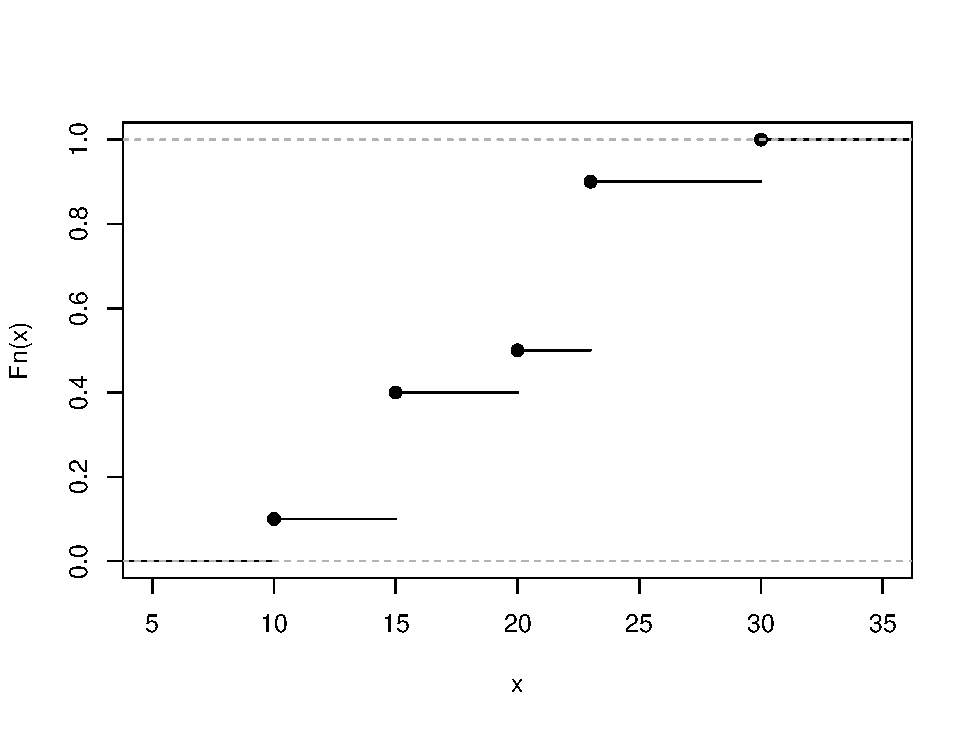
\includegraphics[width=0.6\linewidth]{LossDataAnalytics_files/figure-latex/EDFToy-1} 

}

\caption{Función de Distribución Empírica de un Ejemplo con Datos Ficticios}\label{fig:EDFToy}
\end{figure}

Mostrar código R

\hypertarget{toggleToy}{}
\begin{verbatim}
(xExample <- c(10,rep(15,3),20,rep(23,4),30))
PercentilesxExample <- ecdf(xExample)
plot(PercentilesxExample, main="",xlab="x")
\end{verbatim}

\begin{center}\rule{0.5\linewidth}{0.5pt}\end{center}

\hypertarget{S:MS:QuantileEstimator}{%
\subsubsection{Cuartiles, Percentiles y Cuantiles}\label{S:MS:QuantileEstimator}}

Anteriormente ya hemos visto la \emph{mediana}, que es el número tal que aproximadamente la mitad de un conjunto de datos está por debajo (o por encima). El \textbf{primer cuartil} es el número tal que aproximadamente el 25\% de los datos está debajo de él y el \emph{tercer cuartil} es el número tal que aproximadamente el 75\% de los datos está debajo de él. Un \(100p\) \textbf{percentil} es el número tal que \(100\times p\) por ciento de los datos están debajo de él.

Para generalizar este concepto, se considera una función de distribución \(F(\cdot)\), que puede o no ser continua, y sea \(q\) una fracción para la cual \(0<q<1\). Queremos definir un cuantil, digamos \(q_F\), para que sea un número tal que \(F(q_F) \approx q\). Observe que cuando \(q=0,5\), \(q_F\) es la mediana; cuando \(q=0,25\), \(q_F\) es el primer cuartil, y así sucesivamente. Por lo tanto, un cuantil generaliza los conceptos de mediana, cuartiles y percentiles.

Para ser precisos, para un determinado valor de \(0<q<1\), se define el \(q\)-\textbf{ésimo cuantil} \(q_F\) como \emph{cualquier} número que satisfaga
\begin{equation}
  F(q_F-) \le q \le F(q_F)
  \label{eq:Quantile}
\end{equation}

Aquí, la notación \(F(x-)\) significa evaluar la función \(F(\cdot)\) como el límite por la izquierda.

Para comprender mejor esta definición, veamos algunos casos especiales. Primero, considere el caso en el que \(X\) es una variable aleatoria continua para que la función de distribución \(F(\cdot)\) no tenga puntos de salto, como se ilustra en la Figura \ref{fig:Quantile1}. En esta figura, se muestran algunas fracciones, \(q_1\), \(q_2\) y \(q_3\) con sus cuantiles correspondientes \(q_{F,1}\), \(q_{F,2}\) y \(q_{F,3}\). En cada caso se puede ver que \(F(q_F-)=F(q_F)\), de modo que hay un cuantil único. Al igual que podemos encontrar una inversa de la función de distribución única para cualquier \(0<q<1\), podemos escribir \(q_F=F^{-1}(q)\).

\begin{figure}

{\centering 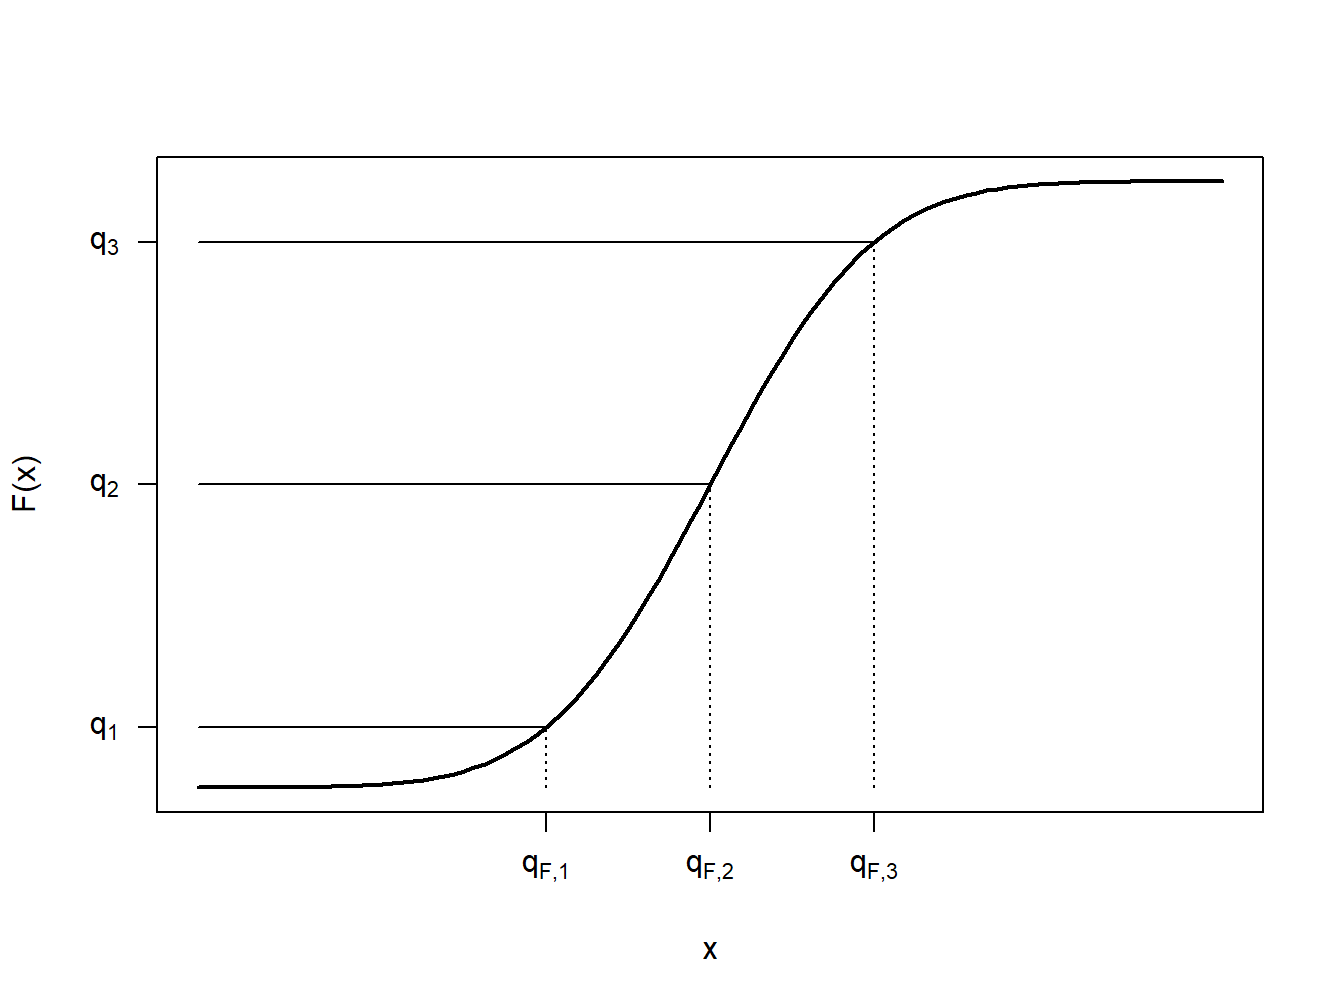
\includegraphics[width=0.6\linewidth]{LossDataAnalytics_files/figure-latex/Quantile1-1} 

}

\caption{Caso de Cuantil Continuo}\label{fig:Quantile1}
\end{figure}

La figura \ref{fig:Quantile2} muestra tres casos de funciones de distribución. El panel izquierdo corresponde al caso continuo recién discutido. El panel central muestra un punto de salto similar a los que ya vimos en la función de distribución empírica de la Figura \ref{fig:EDFToy}. Para el valor de \(q\) que se muestra en este panel, todavía tenemos un valor único del cuantil \(q_F\). Aunque hay muchos valores de \(q\) tales que \(F(q_F-) \le q \le F(q_F)\), para un valor particular de \(q\), solo hay una solución para la ecuación \eqref{eq:Quantile}. El panel de la derecha muestra una situación en la que el cuantil no puede determinarse de manera única para el \(q\) que se muestra, ya que hay un rango de \(q_F\) que satisfacen la ecuación \eqref{eq:Quantile}.

\begin{figure}

{\centering 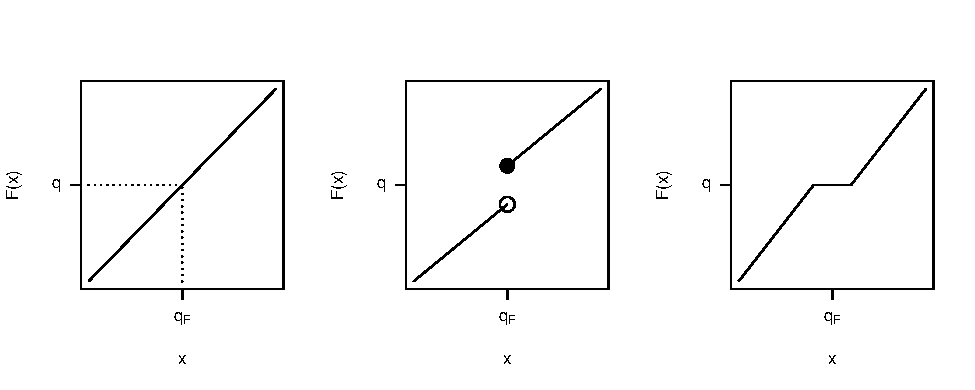
\includegraphics[width=0.9\linewidth]{LossDataAnalytics_files/figure-latex/Quantile2-1} 

}

\caption{Tres Casos de Cuantiles}\label{fig:Quantile2}
\end{figure}

\begin{center}\rule{0.5\linewidth}{0.5pt}\end{center}

\textbf{Ejemplo 4.1.2. Conjunto de Datos Ficticios: Continuación.}
Se determinan los cuantiles correspondientes a los percentiles 20, 50 y 95.

Mostrar la solución del Ejemplo

\leavevmode\hypertarget{toggleExampleSelect.1.2}{}%
\textbf{Solución}.
Se considera la Figura \ref{fig:EDFToy}. El caso de \(q=0,20\) corresponde al panel central, por lo que el percentil 20 es 15. El caso de \(q=0,50\) corresponde al panel derecho, por lo que la mediana es cualquier número entre 20 y 23, ambos inclusive. Muchos paquetes de software usan el promedio de 21,5 (por ejemplo, \texttt{R}, como se ve a continuación). Para el percentil 95, la solución es 30. Podemos ver en el gráfico que 30 también corresponde a los percentiles 99 y 99,99.

\begin{Shaded}
\begin{Highlighting}[]
\FunctionTok{quantile}\NormalTok{(xExample, }\AttributeTok{probs=}\FunctionTok{c}\NormalTok{(}\FloatTok{0.2}\NormalTok{, }\FloatTok{0.5}\NormalTok{, }\FloatTok{0.95}\NormalTok{), }\AttributeTok{type=}\DecValTok{6}\NormalTok{)}
\end{Highlighting}
\end{Shaded}

\begin{verbatim}
##  20%  50%  95% 
## 15.0 21.5 30.0
\end{verbatim}

\begin{center}\rule{0.5\linewidth}{0.5pt}\end{center}

Al tomar un promedio ponderado entre las observaciones de datos, los cuantiles empíricos suavizados pueden asemejarse a los casos como el panel derecho en la Figura \ref{fig:Quantile2}. El \(q\)-ésimo \emph{cuartil empírico suavizado} se define como
\[
\hat{\pi}_q = (1-h) X_{(j)} + h X_{(j+1)}
\]
donde \(j=\lfloor(n+1)q\rfloor\), \(h=(n+1)q-j\), y \(X_{(1)}, \ldots, X_{(n)}\) son los valores ordenados (conocidos como los \emph{estadísticos de orden}) correspondientes a \(X_1, \ldots, X_n\). Cabe señalar que \(\hat{\pi}_q\) es simplemente una interpolación lineal entre \(X_{(j)}\) y \(X_{(j+1)}\).

\textbf{Ejemplo 4.1.3. Conjunto de Datos Ficticios: Continuación.}
Se determinan los percentiles 50-ésimo y 20-ésimo alisados.

Mostrar la solución del Ejemplo

\leavevmode\hypertarget{toggleExampleSelect.1.3}{}%
\textbf{Solución}
Se toma \(n=10\) y \(q=0,5\). De modo que, \(j=\lfloor(11)0,5 \rfloor= \lfloor 5,5 \rfloor=5\) y \(h=(11)(0,5)-5=0,5\). Por tanto, el 50-ésimo cuantil empírico alisado es
\[\hat{\pi}_{0,5} = (1-0,5) X_{(5)} + (0,5) X_{(6)} = 0,5 (20) + (0,5)(23) = 21,5.\]
Ahora se toma \(n=10\) y \(q=0,2\). En este caso, \(j=\lfloor(11)0,2\rfloor=\lfloor 2,2 \rfloor=2\) y \(h=(11)(0,2)-2=0,2\). Entonces, el 20-ésimo cuantil empírico alisado es
\[\hat{\pi}_{0,2} = (1-0,2) X_{(2)} + (0,2) X_{(3)} = 0,2 (15) + (0,8)(15) = 15.\]

\begin{center}\rule{0.5\linewidth}{0.5pt}\end{center}

\hypertarget{estimadores-de-la-densidad}{%
\subsubsection{Estimadores de la Densidad}\label{estimadores-de-la-densidad}}

\textbf{Variable Discreta.} Cuando la variable aleatoria es discreta, estimar la función de masa de probabilidad \(f(x)=\Pr(X = x)\) es sencillo. Simplemente usamos el promedio del indicador \(I(X_i = x)\) en la muestra, definido como

\[f_n(x) = \frac{1}{n} \sum_{i=1}^n I(X_i = x).\]

\textbf{Variable Continua Dentro de un Grupo.} Para una variable aleatoria continua, se considera una formulación discretizada en la que el dominio de \(F(\cdot)\) está dividido por las constantes \(\{c_0 <c_1 <\cdots <c_k\}\) en intervalos de la forma \([c_{j-1}, c_j)\), por \(j = 1, \ldots, k\). Los datos observados se ``agrupan'' en función del intervalo en el que caen. Entonces, podríamos usar la definición básica de la función de masa de probabilidad empírica, o una variación como
\[f_n(x) = \frac{n_j}{n \times (c_j - c_{j-1})}  \ \ \ \ \ \ c_{j-1} \le x < c_j,\]
donde \(n_j\) es el número de observaciones (\(X_i\)) que caen en el intervalo \([c_{j-1}, c_j)\).

\textbf{Variable Continua (no agrupada).} Extendiendo esta noción a situaciones en las que observamos datos individuales, se debe tener en cuenta que siempre podemos crear agrupaciones arbitrarias y usar esta fórmula. Más formalmente, dada \(b>0\) una constante positiva que toma un valor reducido y se conoce como \textbf{ancho de banda (bandwidth)}, se define el estimador de la densidad como

\begin{equation}
  f_n(x) = \frac{1}{2nb} \sum_{i=1}^n I(x-b < X_i \le x + b)
  \label{eq:KDF}
\end{equation}

Mostrar un fragmento de Teoría

\hypertarget{Theorykerneldensity}{}
\begin{center}\rule{0.5\linewidth}{0.5pt}\end{center}

La idea es que el estimador \(f_n(x)\) en la ecuación \eqref{eq:KDF} es la media sobre \(n\) \emph{iid}{ independientes e idénticamente distribuidas } realizaciones de una variable aleatoria con media

\[
\begin{aligned}
\mathrm{E~ } \frac{1}{2b} I(x-b < X \le x + b) &=  \frac{1}{2b}\left(F(x+b)-F(x-b)\right) \\
&=  \frac{1}{2b} \left( \left\{ F(x) + b F^{\prime}(x) + b^2 C_1\right\}
\left\{ F(x) - b F^{\prime}(x) + b^2 C_2\right\} \right) \\
&=  F^{\prime}(x) + b \frac{C_1-C_2}{2} \rightarrow  F^{\prime}(x) = f(x),
\end{aligned}
\]

como \(b \rightarrow 0\). Esto es, \(f_n(x)\) es un estimador asintóticamente insesgado de \(f(x)\) (su esperanza se acerca al valor verdadero a medida que el tamaño de la muestra tiende a infinito). Este desarrollo supone cierta suavización de \(F(\cdot)\), en particular, se deriva dos veces con respecto a \(x\), pero no hace suposiciones sobre la forma de la función de distribución \(F\). Debido a esto, se dice que el estimador de densidad \(f_n\) es \emph{no paramétrico}.

\begin{center}\rule{0.5\linewidth}{0.5pt}\end{center}

Más generalmente, se define el \textbf{estimador núcleo (kernel) de la densidad } de la función de \emph{pdf}{ función de densidad de probabilidad} en \emph{x} como

\begin{equation} 
  f_n(x) = \frac{1}{nb} \sum_{i=1}^n w\left(\frac{x-X_i}{b}\right) ,
  \label{eq:kernelDens}
\end{equation}

donde \(w\) es una función de densidad de probabilidad centrada en 0. Se tiene que tener en cuenta que la ecuación \eqref{eq:KDF} simplemente se convierte en el estimador núcleo de la densidad donde \(w(x) =\frac{1}{2} I(-1 <x \le 1)\), también conocido como \emph{núcleo uniforme}. Otras opciones comunes para \(w\) se muestran en \protect\hyperlink{tab:41}{Table 4.1}.

\[
{\small
\begin{matrix}
\text{Table 4.1: Opciones más comunes como Núcleo del Estimador de la Densidad}\\
\begin{array}{l|cc}
\hline
\text{Kernel} &  w(x) \\
\hline
\text{Uniforme } &  \frac{1}{2}I(-1 < x \le 1) \\
\text{Triángulo} &  (1-|x|)\times I(|x| \le 1) \\
\text{Epanechnikov} & \frac{3}{4}(1-x^2) \times I(|x| \le 1) \\
\text{Gausiana} & \phi(x) \\
\hline
\end{array}\end{matrix}
}
\]

Siendo \(\phi(\cdot)\) la función de densidad normal estándar. Como veremos en el siguiente ejemplo, la elección del ancho de banda \(b\) viene dada por la existencia de un \emph{equilibrio entre sesgo-varianza}, es decir, entre las coincidencias con las características locales de la distribución y la reducción de la dispersión.

\begin{center}\rule{0.5\linewidth}{0.5pt}\end{center}

\textbf{Ejemplo 4.1.4. Fondo Inmobiliario.}
La figura \ref{fig:Density2} muestra un histograma (con rectángulos grises sombreados) de los logaritmo de los costes de los siniestros en propiedades del año 2010. La curva gruesa (azul) representa la densidad estimada con el núcleo gaussiano, donde el ancho de banda se seleccionó automáticamente utilizando una regla ad-hoc basada en el tamaño de la muestra y la dispersión de los datos. Para este conjunto de datos, el ancho de banda resultó ser \(b = 0,3255\). A modo comparativo, la curva discontinua (roja) representa el estimador de la densidad con un ancho de banda igual a 0,1 y la curva verde, más suave, utiliza un ancho de banda de 1. Como se anticipó, el ancho de banda más pequeño (0,1) implica realizar promedios locales sobre menos datos para obtener una mejor idea del comportamiento local, pero al precio de una mayor dispersión. En contraste, el mayor ancho de banda (1) suaviza las fluctuaciones locales, produciendo una curva más suave que puede perder perturbaciones reales en el promedio local. Para aplicaciones actuariales, utilizamos principalmente el estimador núcleo de la densidad para obtener una impresión visual rápida de los datos. Desde esta perspectiva, simplemente puede usarse la regla ad-hoc predeterminada para la selección del ancho de banda, sabiendo que se tiene la capacidad de cambiarla dependiendo de la situación en cuestión.

\begin{figure}

{\centering 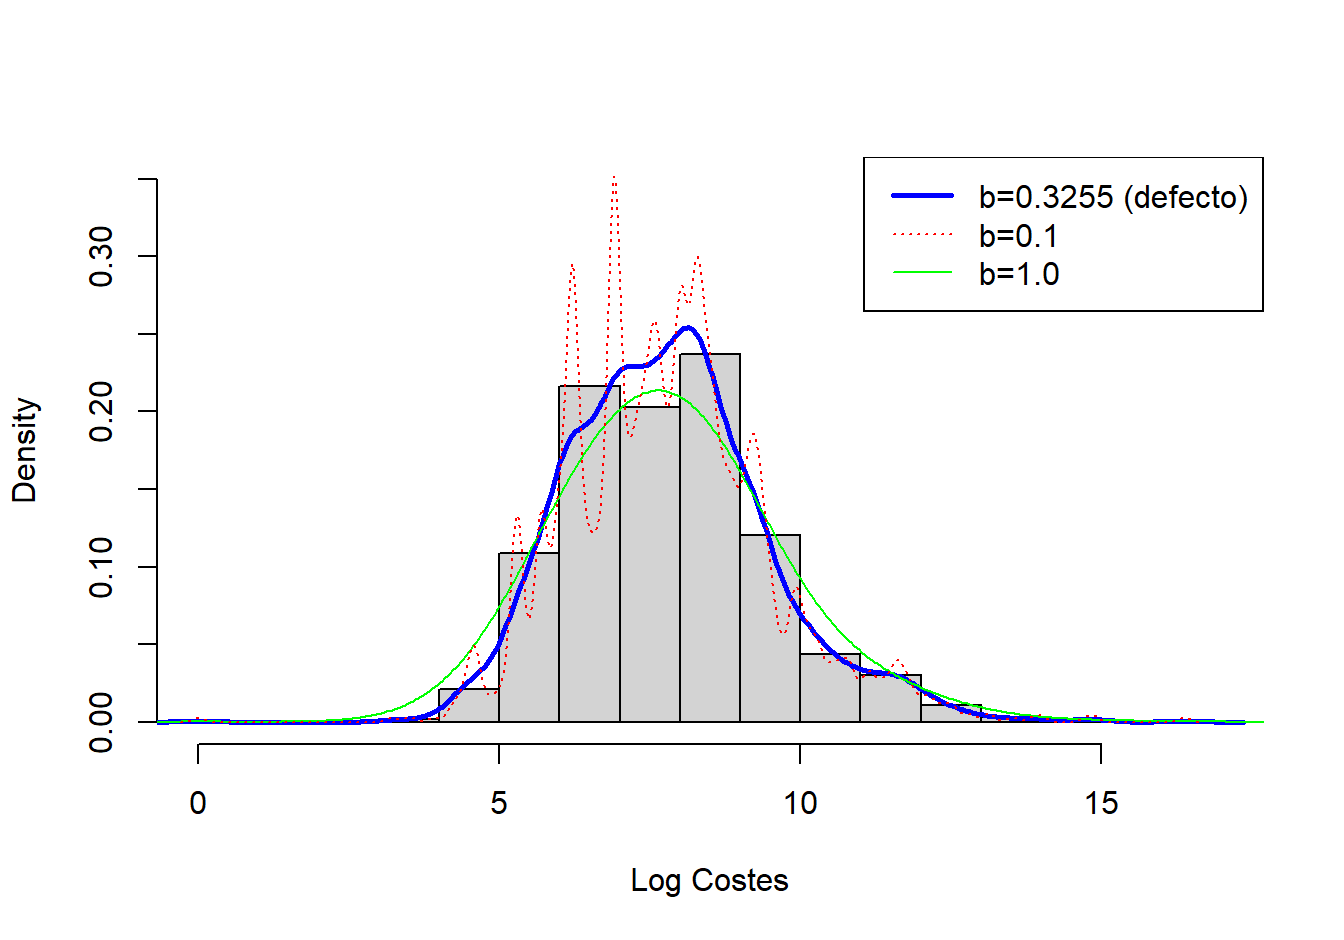
\includegraphics[width=0.7\linewidth]{LossDataAnalytics_files/figure-latex/Density2-1} 

}

\caption{Histograma de los Logaritmo de los Costes de los Siniestros en Propiedades con Estimador Núcleo de la Densidad Superpuesto}\label{fig:Density2}
\end{figure}

Mostrar código R

\hypertarget{togglekpdf}{}
\begin{verbatim}
#Comparación de Densidad
hist(log(ClaimData$Claim), main="", ylim=c(0,.35),xlab="Log Costes", freq=FALSE, col="lightgray")
lines(density(log(ClaimData$Claim)), col="blue",lwd=2.5)
lines(density(log(ClaimData$Claim), bw=1), col="green")
lines(density(log(ClaimData$Claim), bw=.1), col="red", lty=3)
legend("topright", c("b=0.3255 (default)", "b=0.1", "b=1.0"), lty=c(1,3,1),
            lwd=c(2.5,1,1), col=c("blue", "red", "green"), cex=1)
\end{verbatim}

\begin{center}\rule{0.5\linewidth}{0.5pt}\end{center}

Los estimadores no paramétricos de la densidad, como el estimador núcleo, se usan habitualmente en la práctica. Este mismo concepto también se puede ampliar para dar versiones suavizadas de una función de distribución empírica. Dada la definición del estimador núcleo de la densidad, el \emph{estimador núcleo de la función de distribución } se puede obtener como

\[
\begin{aligned}
\hat{F}_n(x) = \frac{1}{n} \sum_{i=1}^n W\left(\frac{x-X_i}{b}\right).\end{aligned}
\]

donde \(W\) es la función de distribución asociada con la densidad del núcleo \(w\). Para ilustrarlo, para el núcleo uniforme, tenemos \(w(y) = \frac{1}{2}I(-1 < y \le 1)\), de modo que

\[
\begin{aligned}
W(y) =
\begin{cases}
0 &            y<-1\\
\frac{y+1}{2}& -1 \le y < 1 \\
1 & y \ge 1 \\
\end{cases}\end{aligned} .
\]

\begin{center}\rule{0.5\linewidth}{0.5pt}\end{center}

\textbf{Ejemplo 4.1.5. Pregunta de Examen Actuarial.}

Se estudian cinco individuos para estimar el tiempo desde el inicio de una enfermedad hasta la muerte. Los tiempos de muerte son:

\[
\begin{array}{ccccc}
2 & 3 & 3 & 3 & 7  \\
\end{array}.
\]

Usando un núcleo triangular con ancho de banda \(2\), calcular la función de densidad estimada en 2,5.

Mostrar la solución del Ejemplo

\leavevmode\hypertarget{toggleExampleSelect.1.5}{}%
\textbf{Solución.}
Para la estimación núcleo de la densidad tenemos
\[f_n(x) = \frac{1}{nb} \sum_{i=1}^n w\left(\frac{x-X_i}{b}\right),\]
donde \(n=5\), \(b=2\), y \(x=2,5\). Para un kernel triangular, \(w(x) = (1-|x|)\times I(|x| \le 1)\). Así,

\[
\begin{array}{c|c|c}
\hline
X_i & \frac{x-X_i}{b} & w\left(\frac{x-X_i}{b} \right) \\
\hline
2 & \frac{2,5-2}{2}=\frac{1}{4} &  (1-\frac{1}{4})(1) = \frac{3}{4} \\
\hline
3 & & \\
3 & \frac{2,5-3}{2}=\frac{-1}{4} & \left(1-\left| \frac{-1}{4} \right| \right)(1) = \frac{3}{4} \\
3 & & \\
\hline
7 & \frac{2,5-7}{2}=-2,25 & (1-|-2,25|)(0) = 0\\
\hline
\end{array}
\]

Entonces la estimación núcleo de la densidad es \[f_n(x) = \frac{1}{5(2)}\left( \frac{3}{4} + (3) \frac{3}{4} + 0 \right) = \frac{3}{10}\]

\begin{center}\rule{0.5\linewidth}{0.5pt}\end{center}

\hypertarget{principio-de-plug-in}{%
\subsubsection{Principio de Plug-in}\label{principio-de-plug-in}}

Una forma de crear un estimador no paramétrico es usar el principio \emph{de analogía} o \emph{plug-in} donde se reemplaza la \emph{cdf} \(F\) desconocida por un estimador conocido como la \emph{cdf} empírica \(F_n\). Por tanto, si estamos tratando de estimar \(\mathrm{E}~\mathrm{g}(X)=\mathrm{E}_F~\mathrm{g}(X)\) para una función genérica \emph{g}, entonces se define un estimador noparamétrico como \(\mathrm{E}_{F_n}~\mathrm{g}(X)=n^{-1}\sum_{i=1}^n\mathrm{g}(X_i)\).

Para ver su funcionamiento, como un caso particular de \emph{g} consideramos la \emph{ratio de eliminación de pérdidas} presentada en la Sección 3.4.1, \[LER(d)=\frac{\mathrm{E~}(\min(X,d) )}{\mathrm{E~}(X)}\] para un deducible fijo \(d\).

\textbf{Ejemplo. 4.1.11. Siniestros con Daños Corporales y Ratio de Eliminación de Pérdidas }

Utilizamos una muestra de 432 siniestros cerrados de automóvil ocurridos en Boston de \citet{derrig2001applications}. Las pérdidas se registran para los pagos por daños corporales derivados en los accidentes de automóvil. Las pérdidas no están sujetas a deducibles, pero están sujetas a varios límites de póliza, también disponibles en los datos. Se obtiene que sólo 17 de 432 (\(\approx\) 4\%) estaban sujetas al límite en la póliza y, por ello, ignoraremos estos datos en esta ilustración.

La pérdida promedio pagada es 6906. Figura \ref{fig:BIClaims} muestra otros aspectos de la distribución.

En concreto, el panel izquierdo muestra la función de distribución empírica, el panel derecho proporciona un gráfico de la densidad no paramétrica.

\begin{figure}

{\centering 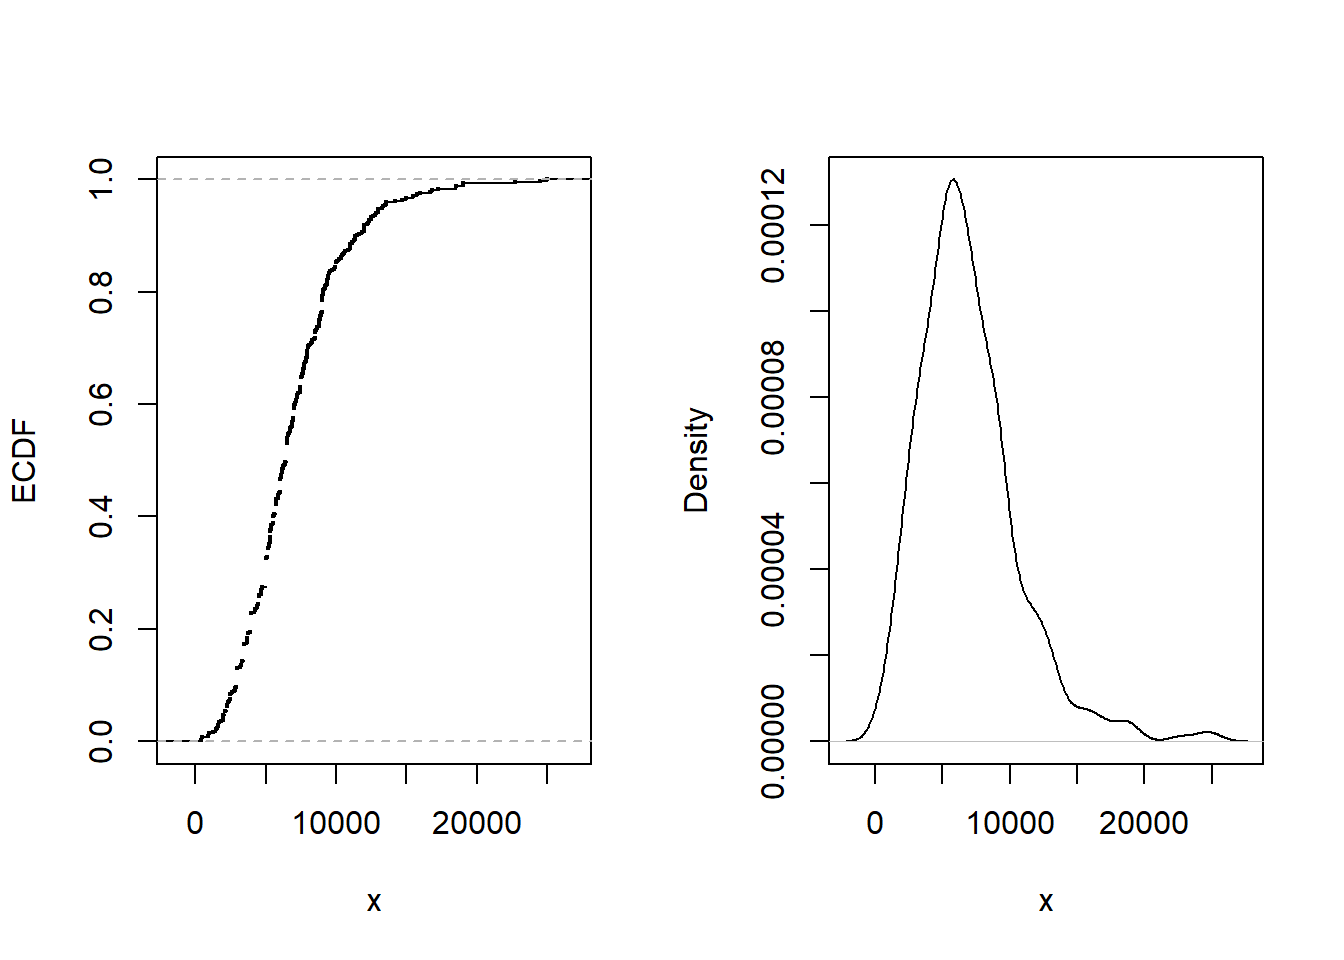
\includegraphics{LossDataAnalytics_files/figure-latex/BIClaims-1} 

}

\caption{Siniestros por daños corporales. La figura de la izquierda proporciona la función de distribución empírica. La figura de la derecha presenta un gráfico de la densidad no paramétrica.}\label{fig:BIClaims}
\end{figure}

El impacto de las pérdidas por lesiones corporales se puede mitigar mediante la imposición de límites o la compra de pólizas de reaseguro (consulte la Sección 10.3). Para cuantificar el impacto de estas herramientas de mitigación de riesgos, es común calcular el índice de eliminación de pérdida o \emph{loss elimination ratio (LER)} como se introdujo en la Sección 3.4.1. La función de distribución no está disponible y se debe estimar de alguna manera. Usando el principio \emph{plug-in}, un estimador no paramétrico se puede definir como
\[
LER_n(d) = \frac{n^{-1} \sum_{i=1}^n \min(X_i,d)}{n^{-1} \sum_{i=1}^n X_i} = \frac{\sum_{i=1}^n \min(X_i,d)}{\sum_{i=1}^n X_i} .
\]

La figura \ref{fig:BIClaims} muestra el estimador \(LER_n(d)\) para varias opciones de \emph{d}. Por ejemplo, si \(d=14.000\), resulta que \(LER_n(14000)\approx\) 0.9768. Imponer un límite de 14.000 significa que esperamos retener 97.68 porcentaje de siniestros.

\begin{figure}

{\centering 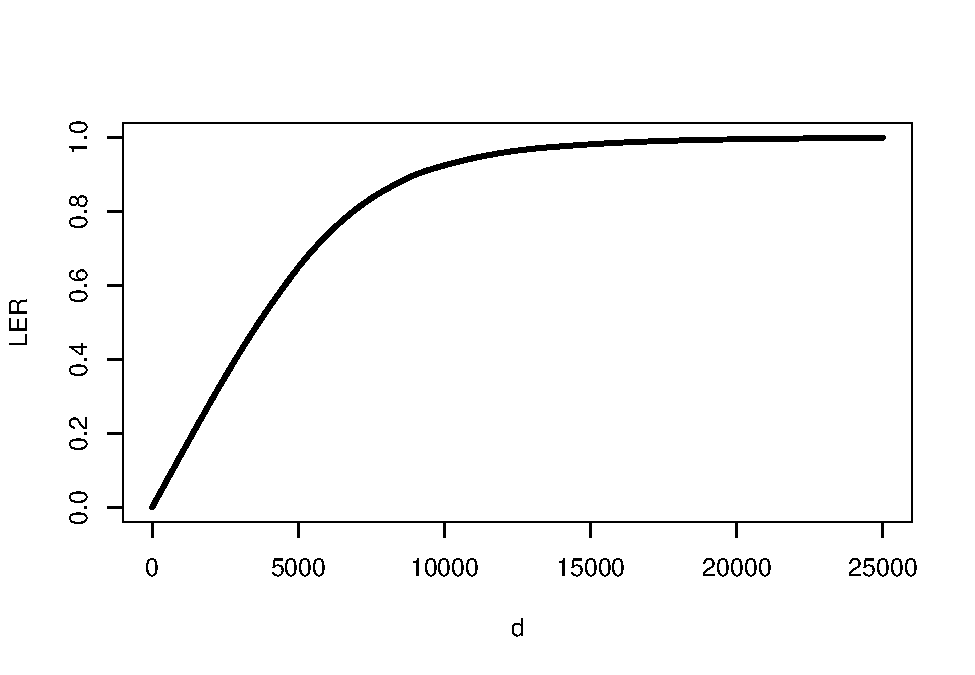
\includegraphics{LossDataAnalytics_files/figure-latex/LER-1} 

}

\caption{LER para siniestros por daños corporales. La figura presenta el índice de eliminación de pérdidas (LER) en función del deducible d.}\label{fig:LER}
\end{figure}

\hypertarget{S:MS:ToolsModelSelection}{%
\subsection{Herramientas para la Selección de Modelos y Diagnósticos}\label{S:MS:ToolsModelSelection}}

En la sección anterior se introdujeron estimadores no paramétricos en los que no se asumía una forma paramétrica sobre las distribuciones subyacentes. Sin embargo, en muchas aplicaciones actuariales, los analistas buscan emplear un ajuste paramétrico de una distribución para facilitar la explicación y la capacidad de extenderla fácilmente a situaciones más complejas, como incluir variables explicativas en un entorno de regresión. Al ajustar una distribución paramétrica, un analista podría intentar usar una distribución gamma para representar un conjunto de datos de pérdida. Sin embargo, otro analista podría preferir usar una distribución de Pareto. ¿Cómo se sabe qué modelo \textbf{seleccionar}?

Se pueden utilizar herramientas no paramétricas para corroborar la selección de modelos paramétricos. Esencialmente, el enfoque es calcular las medidas de resumen seleccionadas bajo un modelo paramétrico ajustado y compararlo con el valor correspondiente bajo el modelo no paramétrico. Como el no paramétrico no asume una distribución específica y es simplemente una función de los datos, se utiliza como punto de referencia para evaluar cómo de bien la distribución/modelo paramétrico representa los datos. Esta comparación puede alertar al analista de deficiencias en el modelo paramétrico y, a veces, señalar formas de mejorar la especificación paramétrica. Los procedimientos orientados a evaluar la validez de un modelo se conocen como \textbf{diagnóstico del modelo}.

\hypertarget{S:MS:GraphComparison}{%
\subsubsection{Comparación Gráfica de Distribuciones}\label{S:MS:GraphComparison}}

Ya hemos visto la técnica de superponer gráficos para fines de comparación. Para reforzar la aplicación de esta técnica, la Figura @ref(fig: ComparisonCDFPDF) compara la distribución empírica con dos distribuciones paramétricas ajustadas. El gráfico izquierdo muestra las funciones de distribución de las distribuciones de siniestros. Los puntos que forman una curva ``en forma de S'' representan la función de distribución empírica en cada observación. La curva azul gruesa proporciona los valores correspondientes para la distribución gamma ajustada y el púrpura claro corresponde a la distribución de Pareto ajustada. Como la distribución de Pareto está mucho más cerca de la función de distribución empírica que la de la gamma, esto nos proporciona una evidencia de que la Pareto es el mejor modelo para este conjunto de datos. El gráfico derecho ofrece información similar para la función de densidad y proporciona un mensaje coherente. Basado (sólo) en estos gráficos, la distribución de Pareto es la opción preferida para el analista.

\begin{figure}

{\centering 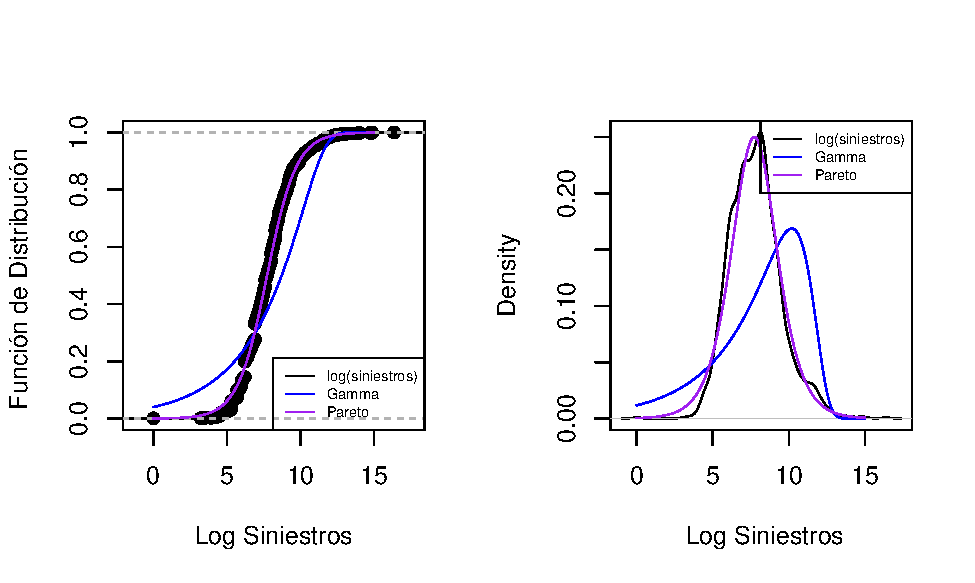
\includegraphics[width=0.8\linewidth]{LossDataAnalytics_files/figure-latex/ComparisonCDFPDF-1} 

}

\caption{Distribución paramétrica versus paramétrica ajustada y funciones de densidad. El gráfico de la izquierda compara las funciones de distribución, con los puntos correspondientes a la distribución empírica, la curva azul gruesa correspondiente a la gamma ajustada y la curva de color púrpura claro correspondiente al Pareto ajustado. El gráfico de la derecha compara estas tres distribuciones resumidas usando funciones de densidad de probabilidad.}\label{fig:ComparisonCDFPDF}
\end{figure}

Otra forma de comparar la idoneidad de dos modelos ajustados es a partir del gráfico de \textbf{probabilidad-probabilidad (\(pp\))}. Un gráfico \(pp\) compara las probabilidades acumuladas en dos modelos. Para nuestro propósito, estos dos modelos son la función de distribución empírica no paramétrica y el modelo paramétrico ajustado. La Figura @ref(fig: PPPlot) muestra los gráficos \(pp\) para los datos del Fondo de la Propiedad. La gamma ajustada está a la izquierda y la Pareto ajustada está a la derecha, en comparación con la misma función de distribución empírica de los datos. La línea recta representa la igualdad entre las dos distribuciones que se comparan, por lo que son deseables los puntos cercanos a la línea. Como se vio en demostraciones anteriores, la Pareto está mucho más cerca de la distribución empírica que la gamma, lo que proporciona evidencia adicional de que la Pareto es el mejor modelo.

\begin{figure}

{\centering 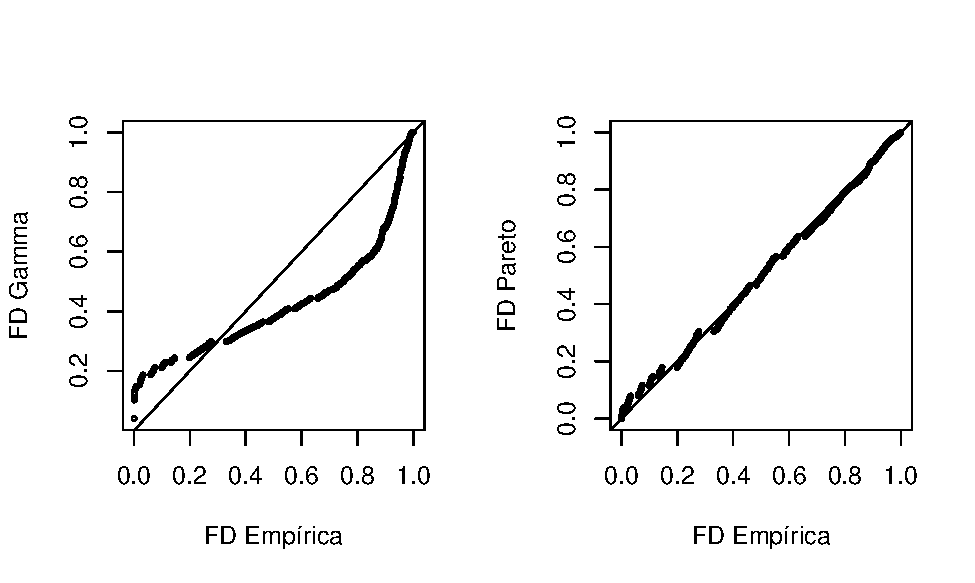
\includegraphics[width=0.8\linewidth]{LossDataAnalytics_files/figure-latex/PPPlot-1} 

}

\caption{Gráficos de Probabilidad-Probabilidad ($pp$). Los ejes horizontales representan la función de distribución empírica en cada observación. En el gráfico izquierdo, la función de distribución correspondiente a la gamma se muestra en el eje vertical. El gráfico de la derecha muestra la distribución de Pareto ajustada. Las líneas de $y=x$ se superponen.}\label{fig:PPPlot}
\end{figure}

Un gráfico \(pp\) es útil en parte porque no se requiere escala artificial, como con la superposición de densidades en la Figura @ref(fig: ComparisonCDFPDF), en la que cambiamos a la escala logarítmica para visualizar mejor los datos. El Capítulo 4 \emph{Suplemento técnico A.1} introduce una variación del diagrama \(pp\) conocido como \emph{curva de Lorenz}; Ésta es una herramienta importante para evaluar la desigualdad de ingresos. Además, los gráficos \(pp\) están disponibles en entornos multivariantes en los que hay más de una variable disponible. Sin embargo, una limitación del gráfico \(pp\) es que, debido a que es un gráfico de funciones de distribución \emph{acumulativas}, a veces puede resultar difícil detectar \emph{dónde} una distribución paramétrica ajustada es deficiente. Como alternativa, se usa frecuentemente un gráfico \textbf{cuantil-cuantil (\(qq\))}, como se muestra en la Figura \ref{fig:QQPlot}.

El gráfico \(qq\) compara dos modelos ajustados a través de sus cuantiles. Al igual que con los gráficos \(pp\), comparamos el modelo no paramétrico con un modelo ajustado paramétrico. Los cuantiles se pueden evaluar en cada punto del conjunto de datos o en una cuadrícula (por ejemplo, en \(0, 0,001, 0,002, \ldots, 0,999, 1.000\)), dependiendo de la aplicación. En la Figura \ref{fig:QQPlot}, para cada punto en la cuadrícula mencionada, el eje horizontal muestra el cuantil empírico y el eje vertical muestra el correspondiente cuantil paramétrico ajustado (gamma para los dos gráficos superiores, Pareto para los dos inferiores). Los cuantiles se trazan en la escala original en los gráficos izquierdos y en la escala logarítmica en los gráficos derechos para permitirnos ver dónde una distribución ajustada es deficiente. La línea recta representa la igualdad entre la distribución empírica y la distribución ajustada. A partir de estos gráficos, nuevamente vemos que en general la Pareto se ajusta mejor que la gamma. Además, el gráfico inferior derecho sugiere que la distribución de Pareto muestra un buen ajuste con valores grandes, pero proporciona un peor ajuste para valores pequeños.

\begin{figure}

{\centering 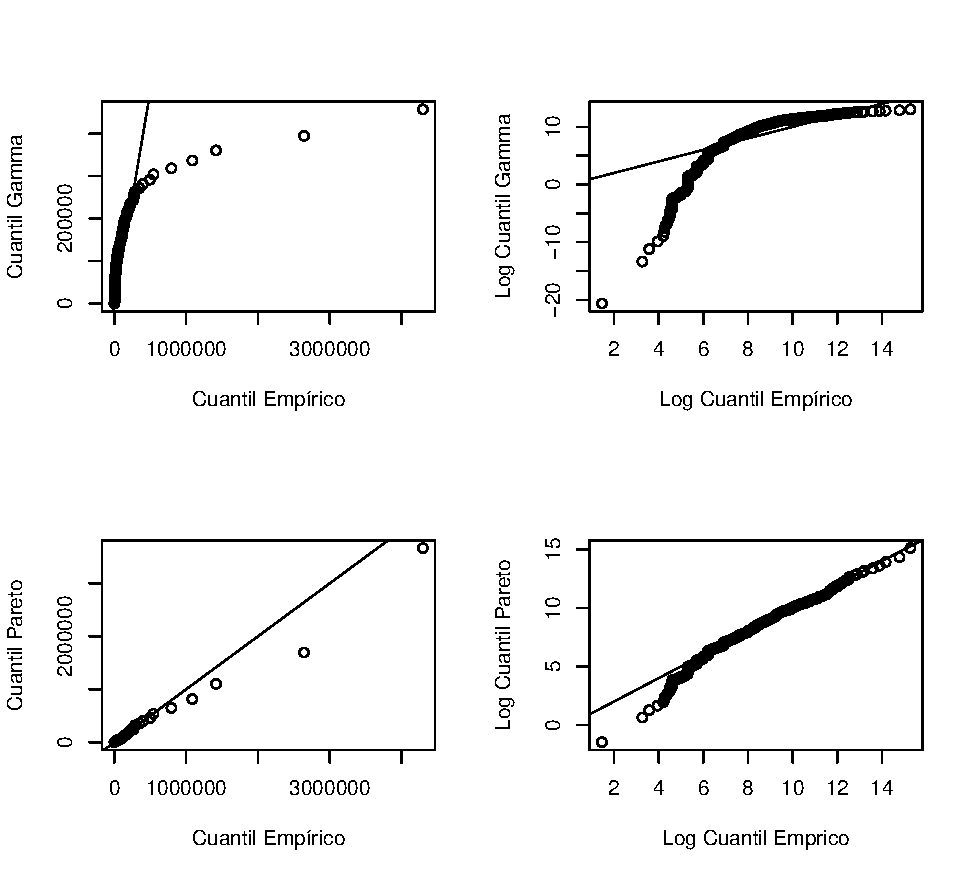
\includegraphics[width=0.8\linewidth]{LossDataAnalytics_files/figure-latex/QQPlot-1} 

}

\caption{Gráficos Cuantil-Cuantil ($qq$). Los ejes horizontales representan los cuantiles empíricos en cada observación. Los gráficos de la derecha están representados sobre una base logarítmica. El eje vertical contiene los cuantiles de las distribuciones ajustadas; los cuantiles gamma están en los gráficos superiores, los cuantiles de Pareto están en los gráficos inferiores.}\label{fig:QQPlot}
\end{figure}

\begin{center}\rule{0.5\linewidth}{0.5pt}\end{center}

\textbf{Ejemplo 4.1.6. Pregunta de Examen Actuarial.}
La siguiente figura muestra un gráfico \(pp\) de una distribución ajustada en comparación con una muestra.

\begin{figure}

{\centering 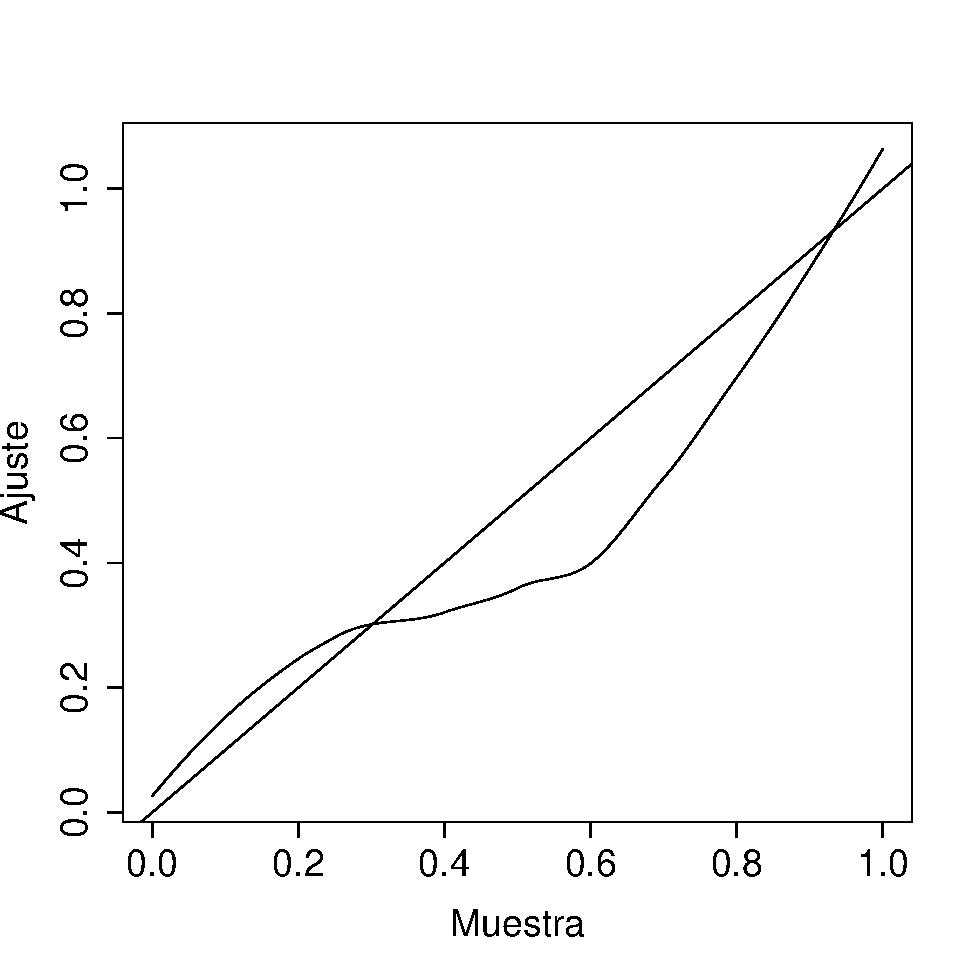
\includegraphics[width=0.4\linewidth]{LossDataAnalytics_files/figure-latex/unnamed-chunk-22-1} 

}

\end{figure}

Comente las dos distribuciones con respecto a la cola izquierda, la cola derecha y las probabilidades medianas.

Mostrar la solución del ejemplo

\leavevmode\hypertarget{toggleExampleSelect.1.6}{}%
\textbf{Solución.}
La cola de la distribución ajustada es demasiado gruesa a la izquierda, demasiado delgada a la derecha, y la distribución ajustada tiene menos probabilidad alrededor de la mediana que la muestra. Para ver esto, recuerde que el gráfico \(pp\) representa gráficamente la distribución acumulada de dos distribuciones en sus ejes (empírica en el eje \(x\) y ajustada en el eje \(y\) en este caso). Para valores pequeños de \(x\), el modelo ajustado asigna una mayor probabilidad de estar por debajo de ese valor que el que se produjo en la muestra (es decir, \(F(x)>F_n(x)\)). Esto indica que el modelo tiene una cola izquierda más pesada que los datos. Para valores grandes de \(x\), el modelo nuevamente asigna una mayor probabilidad de estar por debajo de ese valor y, por lo tanto, menos probabilidad de estar por encima de ese valor (es decir, \(S(x)<S_n(x)\). Esto indica que el modelo tiene una cola derecha más fina que los datos. Además, a medida que avanzamos de 0,4 a 0,6 en el eje horizontal (mirando así el 20\% medio de los datos), el gráfico \(pp\) aumenta aproximadamente de 0,3 a 0,4. Esto indica que el modelo asigna sólo alrededor del 10\% de la probabilidad en este rango.

\begin{center}\rule{0.5\linewidth}{0.5pt}\end{center}

\hypertarget{S:MS:Tools:Stats}{%
\subsubsection{Comparación Estadística de Distribuciones}\label{S:MS:Tools:Stats}}

Para seleccionar un modelo es útil realizar las representaciones gráficas previas. Sin embargo, para mostrar los resultados, puede ser necesario complementar los gráficos con estadísticos de selección que resumen la bondad de ajuste del modelo. La \protect\hyperlink{tab:42}{Tabla 4.2} proporciona tres estadísticos de bondad de ajuste de uso frecuente. En esta tabla, \(F_n\) es la distribución empírica, \(F\) es la distribución ajustada o hipotética, y \(F_i=F(x_i)\).

\[
{\small
\begin{matrix}
\text{Tabla 4.2: Tres Estadísticos de Bondad de Ajuste } \\
\begin{array}{l|cc}
\hline
\text{Estadístico} & \text{Definición} & \text{Expresión Computacional} \\
\hline
\text{Kolmogorov-} & \max_x |F_n(x) - F(x)| & \max(D^+, D^-) \text{ donde} \\
~~~\text{Smirnov} && D^+ = \max_{i=1, \ldots, n} \left|\frac{i}{n} - F_i\right| \\
&& D^- = \max_{i=1, \ldots, n} \left| F_i - \frac{i-1}{n} \right| \\
\text{Cramer-von Mises} & n \int (F_n(x) - F(x))^2 f(x) dx & \frac{1}{12n} + \sum_{i=1}^n \left(F_i - (2i-1)/n\right)^2 \\
\text{Anderson-Darling} & n \int \frac{(F_n(x) - F(x))^2}{F(x)(1-F(x))} f(x) dx & -n-\frac{1}{n} \sum_{i=1}^n (2i-1) \log\left(F_i(1-F_{n+1-i})\right)^2 \\
\hline
\end{array} \\
\end{matrix}
}
\]

El \emph{estadístico de Kolmogorov-Smirnov} es igual a la diferencia absoluta máxima entre la función de distribución ajustada y la función de distribución empírica. En lugar de comparar diferencias entre puntos individuales, el estadístico de \emph{Cramer-von Mises} integra la diferencia entre las funciones de distribución empíricas y ajustadas en todo el rango de valores. El estadístico de \emph{Anderson-Darling} también integra esta diferencia en el rango de valores, aunque ponderada por la inversa de la varianza. Por lo tanto, pone mayor énfasis en las colas de la distribución (es decir, cuando \(F(x)\) o \(1-F(x)=S(x)\) es pequeño).

\begin{center}\rule{0.5\linewidth}{0.5pt}\end{center}

\textbf{Ejemplo 4.1.7. Pregunta de Examen Actuarial (modificada).}
Una muestra de pagos de siniestros es:

\[
\begin{array}{ccccc}
29 & 64 & 90 & 135 & 182  \\
\end{array}
\]

Comparar la distribución empírica de siniestros con una distribución exponencial con una media de \(100\) calculando el valor del estadístico de prueba de Kolmogorov-Smirnov.

Mostrar solución del ejemplo

\leavevmode\hypertarget{toggleExampleSelect.1.7}{}%
\textbf{Solución.}
Para una distribución exponencial con una media de \(100\), la función de distribución acumulada es \(F(x)=1-e^{-x/100}\). Así,
\[
\begin{array}{ccccc}
\hline
x & F(x) & F_n(x) & F_n(x-) & \max(|F(x)-F_n(x)|,|F(x)-F_n(x-)|) \\
\hline
29  & 0,2517 & 0,2 & 0   & \max(0,0517, 0,2517) = 0,2517 \\
64  & 0,4727 & 0,4 & 0,2 & \max(0,0727, 0,2727) = 0,2727 \\
90  & 0,5934 & 0,6 & 0,4 & \max(0,0066, 0,1934) = 0,1934 \\
135 & 0,7408 & 0,8 & 0,6 & \max(0,0592, 0,1408) = 0,1408 \\
182 & 0,8380 & 1   & 0,8 & \max(0,1620, 0,0380) = 0,1620 \\
\hline
\end{array}
\]

El estadístico de la prueba de Kolmogorov-Smirnov es, por lo tanto, \(KS = \max(0,2517, 0,2727, 0,1934, 0,1408, 0,1620) = 0,2727\).

\begin{center}\rule{0.5\linewidth}{0.5pt}\end{center}

\hypertarget{valores-iniciales}{%
\subsection{Valores Iniciales}\label{valores-iniciales}}

Los métodos de momentos y basados en la coincidencia de percentiles son métodos de estimación no paramétricos que proporcionan alternativas a la máxima verosimilitud. Generalmente, la máxima verosimilitud es la técnica preferida porque emplea los datos de manera más eficiente. (Consulte el Capítulo \ref{C:AppC} del Apéndice para obtener las definiciones precisas de eficiencia). Sin embargo, los métodos de momentos y coincidencia de percentiles son útiles porque son más fáciles de interpretar y, por lo tanto, permiten que el actuario o el analista explique los procedimientos a terceros. Además, el procedimiento de estimación numérica (por ejemplo, si se realiza en `R') para la máxima verosimilitud es iterativo y requiere valores iniciales para comenzar el proceso recursivo. Aunque muchos problemas son robustos ante la elección de los valores iniciales, en algunas situaciones complejas, puede ser importante tener un valor inicial cercano al valor óptimo (desconocido). El método de los momentos y la coincidencia de percentiles son técnicas que pueden producir estimaciones deseables sin un elevado coste en términos computacionales y, por lo tanto, pueden usarse como un \emph{valor inicial} para estimar los parámetros por máxima verosimilitud.

\hypertarget{muxe9todo-de-momentos}{%
\subsubsection{Método de Momentos}\label{muxe9todo-de-momentos}}

Con el \textbf{método de momentos}, aproximamos los momentos de la distribución paramétrica utilizando los momentos empíricos (no paramétricos) descritos en la Sección \ref{S:MS:MomentEstimator}. Entonces podemos obtener algebraicamente las estimaciones de los parámetros.
***

\textbf{Ejemplo 4.1.8. Fondo de Propiedad.}
Para el fondo inmobiliario de 2010, hay \(n=1.377\) siniestros individuales (en miles de dólares) con

\[m_1 = \frac{1}{n} \sum_{i=1}^n X_i = 26,62259 \ \ \ \
\text{y} \ \ \ \
 m_2 = \frac{1}{n} \sum_{i=1}^n X_i^2 = 136.154,6 .\]

Ajustar los parámetros de las distribuciones gamma y Pareto utilizando el método de los momentos.

Mostrar solución del ejemplo

\leavevmode\hypertarget{toggleExampleSelect.1.8}{}%
\textbf{Solución.}

Para ajustar una distribución gamma, tenemos \(\mu_1=\alpha\theta\) y \(\mu_2^{\prime}=\alpha(\alpha+1)\theta^2\). Al resolver ambas ecuaciones para obtener la estimación por el método de los momentos, mediante cálculos sencillos se muestra que

\[\alpha = \frac{\mu_1^2}{\mu_2^{\prime}-\mu_1^2}  \ \ \ \text{y} \ \ \  \theta = \frac{\mu_2^{\prime}-\mu_1^2}{\mu_1}.\]

Por lo tanto, los estimadores por el método de los momentos son
\[
\begin{aligned}
\hat{\alpha} &=  \frac{26,62259^2}{136154,6-26,62259^2} = 0,005232809 \\
\hat{\theta} &=  \frac{136154,6-26,62259^2}{26,62259} = 5.087,629.
\end{aligned}
\]

A modo de comparación, los valores obtenidos por máxima verosimilitud son \(\hat{\alpha}_{MLE}=0,2905959\) y \(\hat{\theta}_{MLE}=91,61378\), por lo que hay grandes discrepancias entre las estimaciones obtenidas con los dos procedimientos. Esto es una indicación, como hemos visto antes, de que el modelo gamma no se ajusta bien.

En contraste, ahora se asume una distribución de Pareto, de modo que \(\mu_1 = \theta/(\alpha -1)\) y \(\mu_2^{\prime} = 2\theta^2/((\alpha-1)(\alpha-2) )\). mediante cálculos sencillos se muestra que

\[\alpha = 1+ \frac{\mu_2^{\prime}}{\mu_2^{\prime}-\mu_1^2} \ \ \ \
\text{and} \ \ \ \ \
 \theta = (\alpha-1)\mu_1.\]

Por lo tanto, los estimadores por el método de los momentos son
\[
\begin{aligned}
\hat{\alpha} &=  1+ \frac{136154,6}{136154,6-26,62259^2} = 2,005233 \\
\hat{\theta} &=  (2,005233-1) \cdot 26,62259 = 26,7619
\end{aligned}
\]

Los valores estimados por máxima verosimilitud son \(\hat{\alpha}_{MLE}=0,9990936\) y \(\hat{\theta}_{MLE}=2,2821147\). Es interesante que \(\hat{\alpha}_{MLE}<1\); para la distribución de Pareto, recuerde que \(\alpha<1\) significa que la media es infinita. Esto es otro indicio de que el conjunto de datos de siniestros de la propiedad tiene una distribución de cola larga y pesada.

\begin{center}\rule{0.5\linewidth}{0.5pt}\end{center}

Como se sugiere en el ejemplo anterior, existe flexibilidad con el método de los momentos. Por ejemplo, podríamos haber igualado el segundo y el tercer momento en lugar del primero y el segundo, obteniendo diferentes estimadores. Además, no hay garantía de que exista una solución para cada problema. Adicionalmente, con datos censurados o truncados, hacer coincidir los momentos es solo posible para algunos problemas, y en general, es un escenario más complejo. Finalmente, para distribuciones donde los momentos no existen o son infinitos, el método de momentos no se puede aplicar. Como alternativa, se puede usar la técnica de coincidencia de percentiles.

\hypertarget{coincidencia-de-percentiles}{%
\subsubsection{Coincidencia de percentiles}\label{coincidencia-de-percentiles}}

Bajo el método de \textbf{coincidencia de percentiles}, aproximamos los cuantiles o percentiles de la distribución paramétrica utilizando los cuantiles o percentiles empíricos (no paramétricos) descritos en la Sección \ref{S:MS:QuantileEstimator}.

\begin{center}\rule{0.5\linewidth}{0.5pt}\end{center}

\textbf{Ejemplo 4.1.9. Fondo de propiedad.}

Para el fondo inmobiliario de 2010, ilustramos la correspondencia en cuantiles. En concreto, la distribución de Pareto es intuitivamente sencilla debido a la expresión cerrada para los cuantiles. Recuerde que la función de distribución para la distribución de Pareto es

\[F(x) = 1 - \left(\frac{\theta}{x+\theta}\right)^{\alpha}.\]
Mediante sencillos cálculos se muestra que podemos expresar el cuantil como

\[F^{-1}(q) = \theta \left( (1-q)^{-1/\alpha} -1 \right).\]
for a fraction \(q\), \(0<q<1\).

Determinar las estimaciones de los parámetros de la distribución de Pareto utilizando los cuantiles empíricos 25 y 95.

Mostrar solución del ejemplo

\leavevmode\hypertarget{toggleExampleSelect.1.9}{}%
\textbf{Solución.}

El percentil 25 (el primer cuartil) es \(0,78853\) y el percentil 95 es \(50,98293\) (ambos en miles de dólares). Con dos ecuaciones

\[0,78853 = \theta \left( 1- (1-0,25)^{-1/\alpha} \right) \ \ \ \ \text{y} \ \ \ \ 50,98293 = \theta \left( 1- (1-0,95)^{-1/\alpha} \right)\]
y dos incógnitas, la solución es
\[\hat{\alpha} = 0,9412076 \ \ \ \ \ \text{y} \ \ \ \
\hat{\theta} = 2,205617 .\]
Observamos aquí que se requiere una rutina numérica para estas soluciones ya que no hay una solución analítica disponible. Además, recuerde que las estimaciones de máxima verosimilitud son \(\hat{\alpha}_{MLE}=0,9990936\) y \(\hat{\theta}_{MLE} = 2,2821147\), por lo que la coincidencia de percentiles proporciona una mejor aproximación para la distribución de Pareto que el método de los momentos.

\begin{center}\rule{0.5\linewidth}{0.5pt}\end{center}

\textbf{Ejemplo 4.1.10. Pregunta de Examen Actuarial.}

Te dan:

\begin{enumerate}
\def\labelenumi{(\roman{enumi})}
\tightlist
\item
  Las pérdidas siguen una distribución loglogística con función de distribución acumulada:
  \[F(x) = \frac{\left(x/\theta\right)^{\gamma}}{1+\left(x/\theta\right)^{\gamma}}\]
\item
  La muestra de pérdidas es:
\end{enumerate}

\[
\begin{array}{ccccccccccc}
10 &35 &80 &86 &90 &120 &158 &180 &200 &210 &1500 \\
\end{array}
\]

Estimar \(\theta\) mediante la coincidencia de percentiles, utilizando las estimaciones de percentiles empíricos suavizados del 40 y 80.

Mostrar solución del ejemplo

\leavevmode\hypertarget{toggleExampleSelect.1.10}{}%
\textbf{Solución.}
Con 11 observaciones, tenemos \(j=\lfloor(n+1)q\rfloor = \lfloor 12(0,4) \rfloor = \lfloor 4,8\rfloor=4\) y \(h=(n+1)q-j = 12(0,4)-4=0,8\). Por interpolación, la estimación del percentil 40 empírico suavizado es \(\hat{\pi}_{0,4} = (1-h) X_{(j)} + h X_{(j+1)} = 0,2(86)+0,8(90)=89,2\).

Del mismo modo, para la estimación del percentil 80 empírico suavizado, tenemos \(12(0,8)=9,6\) entonces la estimación es \(\hat{\pi}_{0,8} = 0,4(200)+0,6(210)=206\).

Usando la distribución acumulada loglogística, necesitamos resolver las siguientes dos ecuaciones para los parámetros \(\theta\) y \(\gamma\):
\[0,4=\frac{(89,2/\theta)^\gamma}{1+(89,2/\theta)^\gamma} \ \ \ \text{y} \ \ \ \   0,8=\frac{(206/\theta)^\gamma}{1+(206+\theta)^\gamma}\]

Resolviendo para cada expresión entre paréntesis da \(\frac{2}{3}=(89,2/\theta)^\gamma\) y \(4=(206/\theta)^\gamma\). Sustituyendo la razón de la segunda ecuación en la primera da \(6=(206/89,2)^\gamma \Rightarrow \gamma=\frac{\ln(6)}{\ln(206/89,2)} = 2,1407\). Entonces \(4^{1/2,1407}=206/\theta \Rightarrow \theta=107,8\)

\begin{center}\rule{0.5\linewidth}{0.5pt}\end{center}

Al igual que el método de los momentos, la coincidencia de percentiles es también muy sensible en el sentido de que muchos estimadores pueden basarse en coincidencias de percentiles; por ejemplo, un actuario puede basar la estimación en los percentiles 25 y 95, mientras que otro actuario utiliza los percentiles 20 y 80. En general, estos estimadores serán diferentes y no hay una razón convincente para preferir uno sobre el otro. Por otro lado, como con el método de los momentos, la coincidencia de percentiles es atractiva porque proporciona una técnica que se puede aplicar fácilmente en distintas situaciones y tiene una base intuitiva. Aunque la mayoría de las aplicaciones actuariales usan estimadores de máxima verosimilitud, puede ser conveniente utilizar enfoques alternativos como el método de momentos y la coincidencia de percentiles.

\hypertarget{S:MS:ModelSelection}{%
\section{Selección del Modelo}\label{S:MS:ModelSelection}}

\begin{center}\rule{0.5\linewidth}{0.5pt}\end{center}

En esta sección, se aprende a:

\begin{itemize}
\tightlist
\item
  Describir el proceso iterativo de especificación y de selección de modelo.
\item
  Esquematizar los pasos necesarios para seleccionar un modelo paramétrico.
\item
  Describir los peligros de la selección del modelo basándose únicamente en datos en muestra en comparación con las ventajas de la validación del modelo fuera de muestra.
\end{itemize}

\begin{center}\rule{0.5\linewidth}{0.5pt}\end{center}

En esta sección se subraya la idea de que la selección de modelos es un proceso iterativo en el que los modelos se (re)formulan cíclicamente y se prueban para determinar su idoneidad antes de usarlos para la inferencia. Después de una descripción general, describimos el proceso de selección del modelo basado en:

\begin{itemize}
\tightlist
\item
  un conjunto de datos en muestra o de entrenamiento,
\item
  un conjunto de datos fuera de la muestra o de prueba, y
\item
  un método que combina estos enfoques conocido como \textbf{validación cruzada}.
\end{itemize}

\hypertarget{selecciuxf3n-del-modelo-iterativa}{%
\subsection{Selección del Modelo Iterativa}\label{selecciuxf3n-del-modelo-iterativa}}

En nuestro desarrollo examinamos los datos gráficamente, hipotetizamos la estructura de un modelo y comparamos los datos con un modelo candidato para formular un modelo mejorado. \citet{box1980sampling} lo describe como un \emph{proceso iterativo} el cual se muestra en la Figura \ref{fig:Iterative}.

\begin{figure}

{\centering 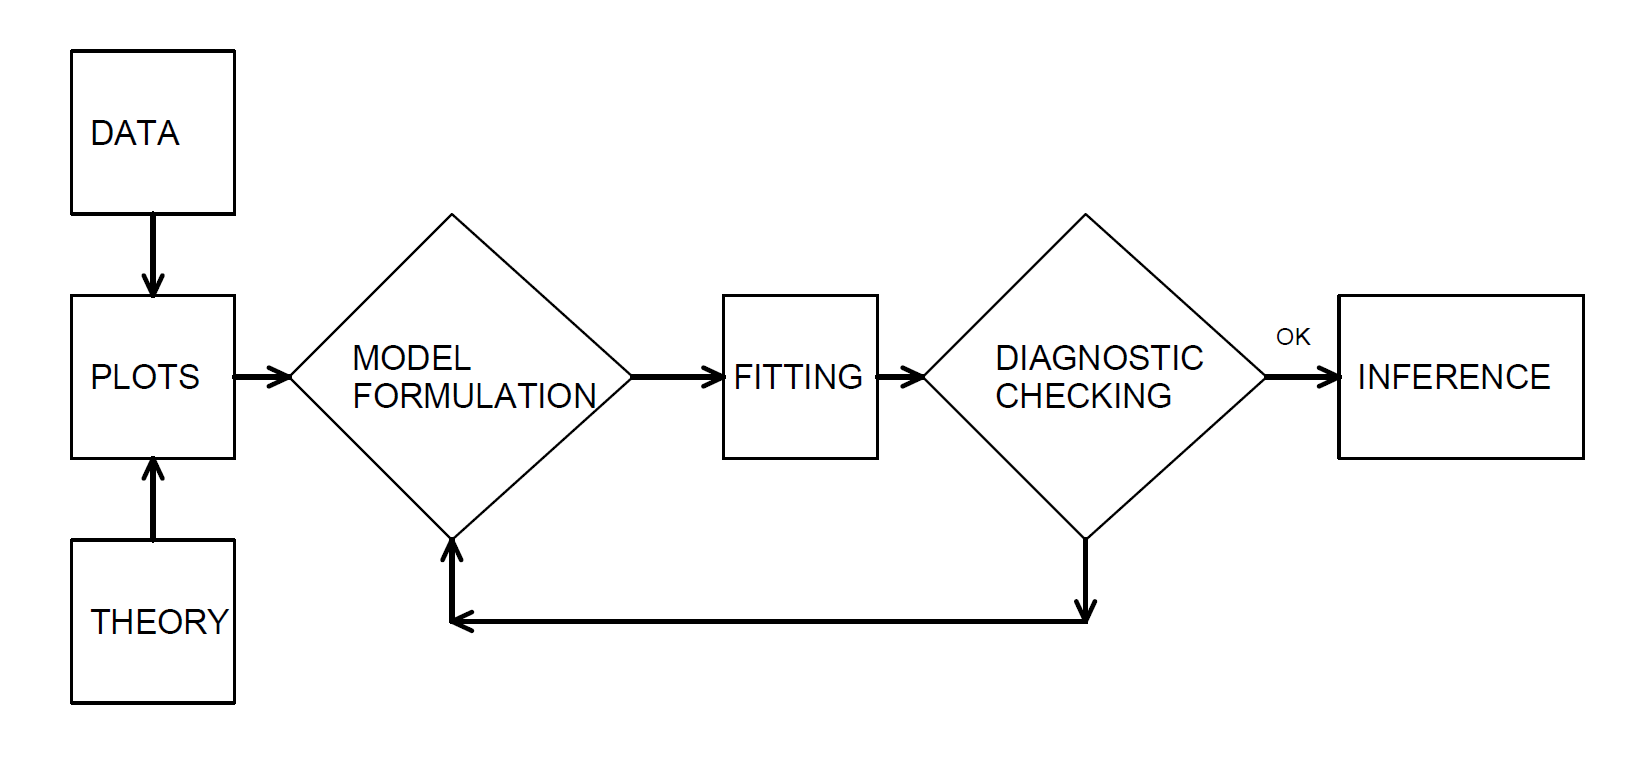
\includegraphics[width=0.8\linewidth]{Figures/F5Iterative} 

}

\caption{El proceso iterativo de especificación del modelo.}\label{fig:Iterative}
\end{figure}

Este proceso iterativo proporciona un mecanismo útil para estructurar el proceso de especificación de un modelo para representar un conjunto de datos.

\begin{enumerate}
\def\labelenumi{\arabic{enumi}.}
\tightlist
\item
  El primer paso, la etapa de formulación del modelo, se logra examinando los datos gráficamente y utilizando el conocimiento previo de las relaciones, como la teoría económica o la práctica de la industria.
\item
  El segundo paso en el proceso iterativo consiste en el ajuste basado en los supuestos del modelo especificado. Estas suposiciones deben ser consistentes con los datos para hacer un uso válido del modelo.
\item
  El tercer paso es el de \emph{comprobación de diagnóstico}; los datos y el modelo deben ser coherentes entre sí antes de poder hacer inferencias adicionales. La verificación de diagnóstico es una parte importante de la formulación del modelo; puede revelar errores cometidos en pasos anteriores y proporcionar formas de corregir estos errores.
\end{enumerate}

El proceso iterativo también enfatiza las habilidades que se necesitan para que la analítica funcione. Primero, se necesita estar dispuesto a resumir la información numéricamente y representarla gráficamente. En segundo lugar, es importante desarrollar una comprensión de las propiedades del modelo. Debe comprenderse cómo se comporta un modelo probabilístico para hacer coincidir un conjunto de datos con él. Tercero, las propiedades teóricas del modelo también son importantes para inferir relaciones generales basadas en el comportamiento de los datos.

\hypertarget{selecciuxf3n-de-modelo-basada-en-un-conjunto-de-datos-de-entrenamiento}{%
\subsection{Selección de Modelo basada en un Conjunto de Datos de Entrenamiento}\label{selecciuxf3n-de-modelo-basada-en-un-conjunto-de-datos-de-entrenamiento}}

Es común referirse a un conjunto de datos utilizado para el análisis como un conjunto de datos \emph{en muestra} o \emph{de entrenamiento}. Las técnicas disponibles para seleccionar un modelo dependen de si los resultados \(X\) son discretos, continuos o un híbrido de los dos, aunque los principios son los mismos.

\textbf{Gráfico y otras medidas de resumen básicas.} Comenzar resumiendo los datos gráficamente y con estadísticos que no se basen en una forma paramétrica específica, como se describe en la Sección \ref{S:MS:NonParInf}. En concreto, es necesario representar gráficamente tanto la distribución empírica como las funciones de densidad. Particularmente, para los datos de pérdidas que contienen muchos ceros y que pueden ser asimétricos, decidir la escala apropiada (por ejemplo, logarítmica) puede representar algunas dificultades. Para datos discretos, a menudo se prefieren las tablas. Determinar los momentos muestrales, como la media y la varianza, así como los cuantiles seleccionados, incluidos el mínimo, el máximo y la mediana. Para datos discretos, la moda (o el valor más frecuente) suele ser útil.

Estos resúmenes, así como el conocimiento de la práctica profesional, permiten proponer uno o más modelos paramétricos candidatos. En general, se debe comenzar con los modelos paramétricos más simples (por ejemplo, la exponencial de un parámetro antes de una gamma de dos parámetros), introduciendo gradualmente más complejidad en el proceso de modelización.

Evaluar el modelo paramétrico candidato numérica y gráficamente. Para los gráficos, se pueden utilizar las herramientas introducidas en la Sección \ref{S:MS:ToolsModelSelection} como los gráficos \(pp\) y \(qq\). Para las evaluaciones numéricas, examinar la importancia estadística de los parámetros e intentar eliminar los parámetros que no proporcionan información adicional.

\textbf{Pruebas de razón de verosimilitud.} Para comparar ajustes del modelo, si un modelo es un subconjunto de otro, entonces se puede utilizar una prueba de razón de verosimilitud; el enfoque general para la prueba de razón de verosimilitud se describe en las Secciones \ref{S:AppA:HT:LRT} y \ref{S:AppC:MLEModelVal}.

\textbf{Estadísticos de bondad del ajuste.} En general, los modelos no son subconjuntos unos de otros, por lo que los estadísticos generales de bondad del ajuste son útiles para comparar modelos. \emph{Los criterios de información} son un tipo de estadístico de bondad de ajuste. Los ejemplos más utilizados son el Criterio de Información de Akaike (\emph{AIC}) y el Criterio de Información Bayesiano (\emph{BIC}) de Schwarz; se mencionan frecuentemente porque pueden generalizarse fácilmente a entornos multivariantes. La Sección \ref{S:AppA:HT:IC} proporciona una descripción de estos estadísticos.

Para seleccionar la distribución adecuada, los estadísticos que comparan un ajuste paramétrico con una alternativa no paramétrica, descritos en la Sección \ref{S:MS:Tools:Stats}, son útiles para la comparación de modelos. Para datos discretos, generalmente se prefiere un estadístico de \emph{bondad de ajuste} (como se describe en la Sección \ref{S:goodness-of-fit}), ya que es más intuitivo y más simple de explicar.

\hypertarget{selecciuxf3n-de-modelo-basada-en-un-conjunto-de-datos-de-prueba}{%
\subsection{Selección de Modelo basada en un Conjunto de Datos de Prueba}\label{selecciuxf3n-de-modelo-basada-en-un-conjunto-de-datos-de-prueba}}

\textbf{Validación del modelo} es el proceso de confirmar que el modelo propuesto es apropiado, especialmente a la luz de los propósitos de la investigación. Una limitación importante del proceso de selección de modelos basado solo en datos de muestra es que puede ser susceptible a \emph{indagación de datos (data-snooping)}, es decir, ajustar una gran cantidad de modelos a un solo conjunto de datos. Al analizar una gran cantidad de modelos, podemos sobreajustar los datos y subestimar la variación natural en nuestra representación.

Seleccionar un modelo basado solo en datos de muestra tampoco es compatible con el objetivo de la \textbf{inferencia predictiva}. Particularmente, en aplicaciones actuariales nuestro objetivo es hacer declaraciones sobre la \emph{nueva} experiencia en lugar de sobre el conjunto de datos disponible. Por ejemplo, utilizamos la experiencia de siniestros de un año para desarrollar un modelo que se pueda usar para fijar el precio de los contratos de seguro para el año siguiente. Como analogía, podemos pensar en el conjunto de datos de entrenamiento como experiencia de un año que se utiliza para predecir el comportamiento del conjunto de datos de prueba del próximo año.

Podemos superar estas limitaciones utilizando una técnica a veces conocida como \textbf{validación fuera de muestra}. La situación ideal es tener disponibles dos conjuntos de datos, uno para entrenamiento o desarrollo del modelo y otro para prueba o validación del modelo. Inicialmente desarrollamos uno o varios modelos en el primer conjunto de datos que llamamos nuestros modelos \emph{candidatos}. Luego, el rendimiento relativo de los modelos candidatos se puede medir en el segundo conjunto de datos. De esta manera, los datos utilizados para validar el modelo no se ven afectados por los procedimientos utilizados para formular el modelo.

\textbf{División aleatoria de los datos.} Desafortunadamente, rara vez estarán disponibles dos conjuntos de datos para el investigador. Sin embargo, podemos implementar el proceso de validación dividiendo el conjunto de datos en submuestras de \textbf{entrenamiento} y \textbf{prueba}, respectivamente. La Figura \ref{fig:ModelValidation} ilustra la división de los datos.

\begin{figure}

{\centering 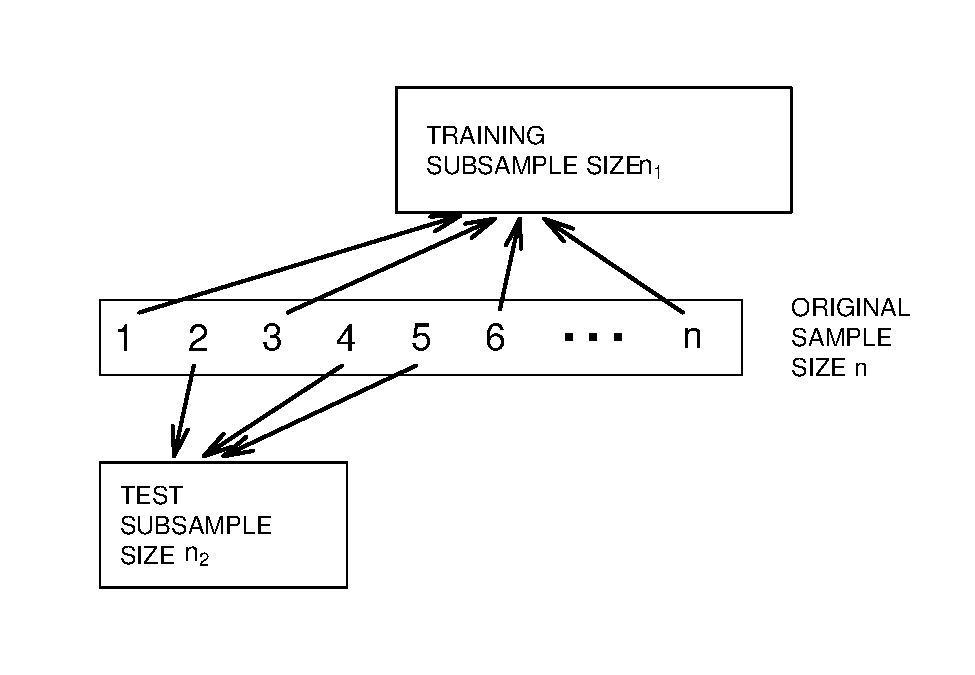
\includegraphics[width=0.6\linewidth]{LossDataAnalytics_files/figure-latex/ModelValidation-1} 

}

\caption{Validación del modelo. Un conjunto de datos se divide aleatoriamente en dos submuestras.}\label{fig:ModelValidation}
\end{figure}

Diferentes proporciones se recomiendan para la asignación a las muestras de entrenamiento y prueba. \citet{snee1977validation} sugiere que la división de datos no se realice a menos que el tamaño de la muestra sea moderadamente grande. Las pautas de \citet{picard1990data} muestran que cuanto mayor sea el número de parámetros a estimar, mayor será la proporción de observaciones necesarias para la submuestra de entrenamiento del modelo.

\textbf{Estadísticos de validación del modelo.} Gran parte de la literatura que respalda el establecimiento de un proceso de validación del modelo se basa en modelos de regresión y clasificación que puede considerarse como un problema \emph{input-output} (\citet{james2013introduction}). Es decir, tenemos varias entradas \(x_1,\ldots,x_k\) que están relacionadas con una salida \(y\) a través de una función como

\[y=\mathrm{g}\left(x_1,\ldots,x_k\right).\]

Se utiliza la muestra de entrenamiento para desarrollar una estimación de \(\mathrm{g}\), digamos, \(\hat{\mathrm{g}}\), y luego se calibra la distancia entre los resultados observados y las predicciones usando un criterio de la forma
\begin{equation}
\sum_i \mathrm{d}(y_i,\hat{\mathrm{g}}\left(x_{i1}, \ldots, x_{ik}\right) ) .
\label{eq:OutSampleCriter}
\end{equation}

Aquí, la suma \emph{i} se realiza sobre los datos de prueba. En muchas aplicaciones de regresión es común usar la distancia euclidiana al cuadrado de la forma \(\mathrm{d}(y_i,\mathrm{g})=(y_i-\mathrm{g})^2\). En aplicaciones actuariales, la distancia euclidiana \(\mathrm{d}(y_i,\mathrm{g})=|y_i-\mathrm{g}|\) a menudo se prefiere debido a la naturaleza asimétrica de los datos (valores extremos grandes de \(y\) pueden tener un gran impacto en la medida). El Capítulo \ref{C:PremiumFoundations} describe otra medida, el \emph{índice de Gini}, que es útil en aplicaciones actuariales, particularmente cuando hay una gran proporción de ceros en los datos de siniestros (correspondientes a ningún siniestro).

\textbf{Selección de una distribución.} Nuestro enfoque hasta ahora ha sido seleccionar una distribución para un conjunto de datos que pueda usarse para la modelización actuarial sin entradas adicionales \(x_1,\ldots,x_k\). Incluso en este problema más fundamental, el enfoque de validación del modelo es adecuado. Si basamos toda la inferencia solo en datos de la muestra, entonces la tendencia es seleccionar modelos más complicados de lo necesario. Por ejemplo, se podría seleccionar una distribución con cuatro parámetros como la GB2, distribución beta generalizada de segundo tipo, cuando solo se necesita una Pareto con dos parámetros. Criterios de información como \emph{AIC}{ criterio de información de Akaike} y \emph{BIC}{ criterio de información Bayesiano} que incluyen penalizaciones a la complejidad del modelo y, por lo tanto, proporcionan cierta protección, con el uso de una muestra de prueba son la mejor garantía para lograr modelos parsimoniosos. Una cita a menudo atribuida a Albert Einstein, indica queremos ``utilizar el modelo más simple (sencillo) posible pero no el más simple (simplón)''.

\hypertarget{selecciuxf3n-del-modelo-basada-en-validaciuxf3n-cruzada}{%
\subsection{Selección del Modelo basada en Validación Cruzada}\label{selecciuxf3n-del-modelo-basada-en-validaciuxf3n-cruzada}}

Aunque la validación fuera de la muestra es el estándar más valioso en la modelización predictiva, no siempre es práctico hacerlo. La razón principal es que tenemos tamaños de muestra limitados y el criterio de selección de modelo fuera de muestra en la ecuación \eqref{eq:OutSampleCriter} depende de una división \emph{aleatoria} de los datos. Lo anterior genera que diferentes analistas, incluso cuando utilizan el mismo conjunto de datos y el mismo enfoque para la modelización, puedan seleccionar diferentes modelos. Esto puede ocurrir en aplicaciones actuariales ya que se utilizan conjuntos de datos asimétricos en los que hay una elevada probabilidad de obtener algunos valores muy grandes y los valores grandes pueden tener un gran impacto en las estimaciones de los parámetros.

\textbf{Procedimiento de Validación Cruzada.} Alternativamente, se puede utilizar \textbf{validación cruzada}, de la siguiente forma.

-El procedimiento se inicia mediante el uso de un mecanismo aleatorio para dividir los datos en \emph{K} subconjuntos denominados \emph{pliegues}. Los analistas suelen utilizar de 5 a 10.
-Después se utilizan las primeras \emph{K} -1 submuestras para estimar los parámetros del modelo. Luego, se ``predicen'' los resultados para la submuestra \emph{K}-ésima y se aplica una medida como las definidas en la ecuación \eqref{eq:OutSampleCriter} para describir el ajuste.
-Ahora, se repite para cada una de las \emph{K} submuestras, utilizando un estadístico acumulativo fuera de muestra para describir el ajuste.

Repetir estos pasos para varios modelos candidatos y elegir el modelo con el estadístico acumulativo fuera de muestra más bajo.

La validación cruzada se utiliza frecuentemente porque retiene la naturaliza predictiva del proceso de validación del modelo fuera de muestra pero, debido a la reutilización de los datos, es más estable que el procedimiento basado en muestras aleatorias.

\hypertarget{S:MS:ModifiedData}{%
\section{Estimación utilizando Datos Modificados}\label{S:MS:ModifiedData}}

\begin{center}\rule{0.5\linewidth}{0.5pt}\end{center}

En esta sección, se aprende a:

\begin{itemize}
\tightlist
\item
  Describir datos agrupados, censurados y truncados.
\item
  Estimar distribuciones paramétricas basadas en datos agrupados, censurados y truncados
\item
  Estimar distribuciones no paramétricas basadas en datos agrupados, censurados y truncados
\end{itemize}

\begin{center}\rule{0.5\linewidth}{0.5pt}\end{center}

\hypertarget{estimaciuxf3n-paramuxe9trica-usando-datos-modificados}{%
\subsection{Estimación Paramétrica usando Datos Modificados}\label{estimaciuxf3n-paramuxe9trica-usando-datos-modificados}}

La teoría básica y muchas aplicaciones se basan en observaciones \emph{individuales} que son ``\emph{completas}'' y ``\emph{no modificadas}'', como hemos visto en la sección anterior. La sección \ref{S:MaxLikeEstimation} introduce el concepto de observaciones que están ``\emph{modificadas}'' debido a dos tipos comunes de limitaciones: \textbf{censura} y \textbf{truncamiento}. Por ejemplo, se suele pensar que un deducible o franquicia de seguros genera datos truncados (desde la izquierda) o los límites de la póliza genera datos censurados (desde la derecha). Este es el punto de vista del asegurador primario (el vendedor del seguro). Sin embargo, como veremos en el Capítulo \ref{C:PortMgt}, un reasegurador (un asegurador de una compañía de seguros) no puede observar reclamaciones menores a una cantidad, solo si existe la reclamación, un ejemplo de censura desde la izquierda. En esta sección se cubre toda la gama de alternativas. Específicamente, esta sección abordará los métodos de estimación paramétrica para tres alternativas a los datos individuales, completos y no modificados: \textbf{datos censurados por intervalos} disponibles solo en grupos, datos limitados o \textbf{censurados}, y datos que no pueden ser observados debido a \textbf{truncamiento}.

\hypertarget{S:MS:GroupedData}{%
\subsubsection{Estimación Paramétrica utilizando Datos Agrupados}\label{S:MS:GroupedData}}

Considerar una muestra de tamaño \(n\) observada a partir de la distribución \(F(\cdot)\), pero en grupos, de modo que solo conocemos el grupo en el que cayó cada observación, no el valor exacto. Esto se conoce como datos \textbf{agrupados} o \textbf{censurados por intervalos}. Por ejemplo, podemos estar viendo dos años consecutivos de registros anuales de empleados. Las personas empleadas en el primer año pero no en el segundo se han ido en algún momento durante el año. Con una fecha de salida exacta (datos individuales), podríamos calcular la cantidad de tiempo que estuvieron en la empresa. Sin la fecha de salida (datos agrupados), solo sabemos que partieron en algún momento durante un intervalo de un año.

Formalizando esta idea, supongamos que hay \(k\) grupos o intervalos delimitados por límites \(c_0<c_1<\cdots<c_k\). Para cada observación solo se conoce el intervalo en el que cayó (por ejemplo, \((c_{j-1},c_j)\)), no el valor exacto. Por lo tanto, solo sabemos el número de observaciones en cada intervalo. Las constantes \(\{c_0<c_1<\cdots<c_k\}\) forman alguna partición del dominio de \(F(\cdot)\). Entonces, la probabilidad de que una observación \(X_i\) caiga en el intervalo \(j\)-ésimo es
\[\Pr\left (X_i \in (c_{j-1},c_j] \right)=F(c_j)-F(c_{j-1}).\]

La función de masa de probabilidad correspondiente para una observación es

\[
\begin{aligned}
f(x) &=
\begin{cases}
F(c_1) - F(c_{0}) &   \text{if }\ x \in (c_{0}, c_1]\\
\vdots & \vdots \\
F(c_k) - F(c_{k-1}) &   \text{if }\ x \in (c_{k-1}, c_k]\\
\end{cases} \\
&= \prod_{j=1}^k \left\{F(c_j) - F(c_{j-1})\right\}^{I(x \in (c_{j-1}, c_j])}
\end{aligned}
\]

Ahora, se define \(n_j\) como el número de observaciones que caen en el intervalo \(j\)-ésimo, \((c_{j-1}, c_j]\). Por lo tanto, la función de verosimilitud (con respecto al(los) parámetro(s) \(\theta\)) es

\[
\begin{aligned}
\mathcal{L}(\theta) = \prod_{j=1}^n f(x_i) = \prod_{j=1}^k \left\{F(c_j) - F(c_{j-1})\right\}^{n_j}
\end{aligned}
\]
y el logaritmo de la función de verosimilitud es
\[
\begin{aligned}
L(\theta) = \ln \mathcal{L}(\theta) = \ln \prod_{j=1}^n f(x_i) = \sum_{j=1}^k n_j \ln \left\{F(c_j) - F(c_{j-1})\right\}
\end{aligned}
\]

Entonces, maximizar la función de verosimilitud (o, de manera equivalente, maximizar el logaritmo de la función de verosimilitud) generará los estimadores por máxima verosimilitud para los datos agrupados.

\textbf{Ejemplo 4.3.1. Pregunta de Examen Actuarial.}

Te dan:

\begin{enumerate}
\def\labelenumi{(\roman{enumi})}
\tightlist
\item
  Las pérdidas siguen una distribución exponencial con media \(\theta\).
\item
  Una muestra aleatoria de 20 pérdidas se distribuye de la siguiente manera:
  \[
  {\small
  \begin{array}{l|c}
  \hline
  \text{Rango de Pérdidas} & \text{Frecuencia} \\
  \hline
  [0,1000] & 7 \\
  (1000,2000] & 6 \\
  (2000,\infty) & 7 \\
  \hline
  \end{array}
  }
  \]
\end{enumerate}

Calcular la estimación máximo verosímil de \(\theta\).

Mostrar solución del ejemplo

\leavevmode\hypertarget{toggleExampleSelect.3.1}{}%
\textbf{Solución.}
\[
\begin{aligned}
\mathcal{L}(\theta) &= F(1000)^7[F(2000)-F(1000)]^6[1-F(2000)]^7 \\
&= (1-e^{-1000/\theta})^7(e^{-1000/\theta} - e^{-2000/\theta})^6(e^{-2000/\theta})^7 \\
&= (1-p)^7(p-p^2)^6(p^2)^7 \\
&= p^{20}(1-p)^{13}
\end{aligned}
\]

donde \(p=e^{-1000/\theta}\). Maximizar esta expresión con respecto a \(p\) es equivalente a maximizar la verosimilitud con respecto a \(\theta\). El máximo ocurre en \(p=\frac{20}{33}\) y entonces \(\hat{\theta}=\frac{-1000}{\ln(20/33)}=1996,90\).

\begin{center}\rule{0.5\linewidth}{0.5pt}\end{center}

\hypertarget{datos-censurados}{%
\subsubsection{Datos Censurados}\label{datos-censurados}}

La \textbf{censura} ocurre cuando registramos solo un valor límite para una observación. La forma más común es \textbf{censurar por la derecha}, en la cual registramos el valor \emph{más pequeño} entre el ``verdadero'' de la variable dependiente y una variable de censura. Usando notación, supongamos que \(X\) representa un resultado de interés, como la pérdida debido a un evento asegurado o el tiempo hasta un evento. La cuantía de censura se denota como \(C_U\). Como observaciones censuradas por la derecha, registramos \(X_U^{\ast}=\min(X,C_U)=X\wedge C_U\). También registramos si se ha producido o no la censura. Supongamos que \(\delta_U=I(X \leq C_U)\) sea una variable binaria que es 0 si se produce la censura y 1 si no es así.

Para el ejemplo que vimos en la Sección \ref{S:PolicyLimits}, \(C_U\) puede representar el límite superior de cobertura de una póliza de seguro (utilizamos \(u\) para el límite superior en esa sección). La pérdida puede exceder el valor \(C_U\), pero la aseguradora solo guarda \(C_U\) en sus registros como la cantidad pagada y no guarda el valor de la pérdida real \(X\).

De manera similar, con la \textbf{censura por la izquierda}, registramos el valor \emph{más grande} entre la variable de interés y la variable de censura. Si se usa \(C_L\) para representar la cantidad de censura, registramos \(X_L^{\ast}=\max(X,C_L)\) junto con el indicador de censura \(\delta_L=I(X\geq C_L)\).

Como ejemplo, tenemos una breve introducción al reaseguro, seguro para aseguradores, en la Sección \ref{S:Chap3Reinsurance} y se verá más en el Capítulo \ref{C:PortMgt}. Supongamos que una reaseguradora cubrirá las pérdidas de la aseguradora mayores a \(C_L\); esto significa que el reasegurador es responsable del exceso de \(X_L^{\ast}\) sobre \(C_L\). Usando notación, esto es \(Y=X_L^{\ast}-C_L\). Para ver esto, primero considere el caso donde la pérdida del titular de la póliza \(X<C_L\). Luego, el asegurador pagará el siniestro completo y \(Y=C_L-C_L=0\), sin pérdida para el reasegurador. Para el segundo caso, si la pérdida \(X\ge C_L\), entonces \(Y=X-C_L\) representa las reclamaciones retenidas por el reasegurador. Dicho de otra manera, si ocurre una pérdida, el reasegurador registra la cuantía real si excede del límite \(C_L\) o, de lo contrario, solo registra que tuvo una pérdida de \(0\).

\hypertarget{datos-truncados}{%
\subsubsection{Datos Truncados}\label{datos-truncados}}

Las observaciones censuradas se registran para su estudio, aunque de forma limitada. En contraste, los resultados \textbf{truncados} son un tipo de datos ausentes. Un resultado se trunca potencialmente cuando la disponibilidad de una observación depende del resultado.

En el seguro, es común que las observaciones sean \textbf{truncadas por la izquierda} en \(C_L\) cuando la cantidad es
\[
\begin{aligned}
Y &=
\left\{
\begin{array}{cl}
\text{nosotros no observamos }X & X < C_L \\
X & X \geq C_L
\end{array}
\right.\end{aligned} .
\]

En otras palabras, si \(X\) es menor que el umbral \(C_L\), entonces no se observa.

Para un ejemplo que vimos en la Sección \ref{S:PolicyDeduct}, \(C_L\) puede representar el deducible de una póliza de seguro (utilizamos \(d\) para el deducible en esa sección). Si la pérdida asegurada es menor que el deducible, entonces el asegurador no puede observar ni registrar la pérdida. Si la pérdida excede el deducible, el exceso de \(X-C_L\) es el siniestro que cubre la aseguradora. En la Sección \ref{S:PolicyDeduct}, definimos la pérdida por pago como
\[
Y^{P} = \left\{ \begin{matrix}
\text{Indefinido} & X \le d \\
X - d & X > d 
\end{matrix} \right. ,
\]
de modo que si una pérdida excede un deducible, registramos la cuantía en exceso \(X-d\). Esto es muy importante cuando se consideran las cuantías que pagará la aseguradora. Sin embargo, para propósitos de estimación de esta sección, importa poco si restamos una constante conocida como \(C_L=d\). Entonces, para nuestra variable truncada \(Y\), usamos la convención más simple y no restamos \(d\).

De manera similar para datos \textbf{truncados por la derecha}, si \(X\) excede un umbral \(C_U\), entonces no se observa. En este caso, la cantidad es
\[
\begin{aligned}
Y &=
\left\{
\begin{array}{cl}
X & X \leq C_U \\
\text{nosotros no observamos }X & X > C_U.
\end{array}
\right.\end{aligned}
\]

Los ejemplos clásicos de truncamiento por la derecha incluyen \(X\) como medida de distancia a una estrella. Cuando la distancia excede un cierto nivel \(C_U\), la estrella ya no es observable.

La Figura \ref{fig:CensorTrunc} compara observaciones truncadas y censuradas. Los valores de \(X\) que son mayores que el límite ``superior'' \(C_U\) no se observan (truncados a la derecha), mientras que los valores de \(X\) que son menores que el límite ``inferior'' \(C_L\) se observan, pero se observan como \(C_L\) en lugar del valor real de \(X\) (censura a la izquierda).

\begin{figure}

{\centering 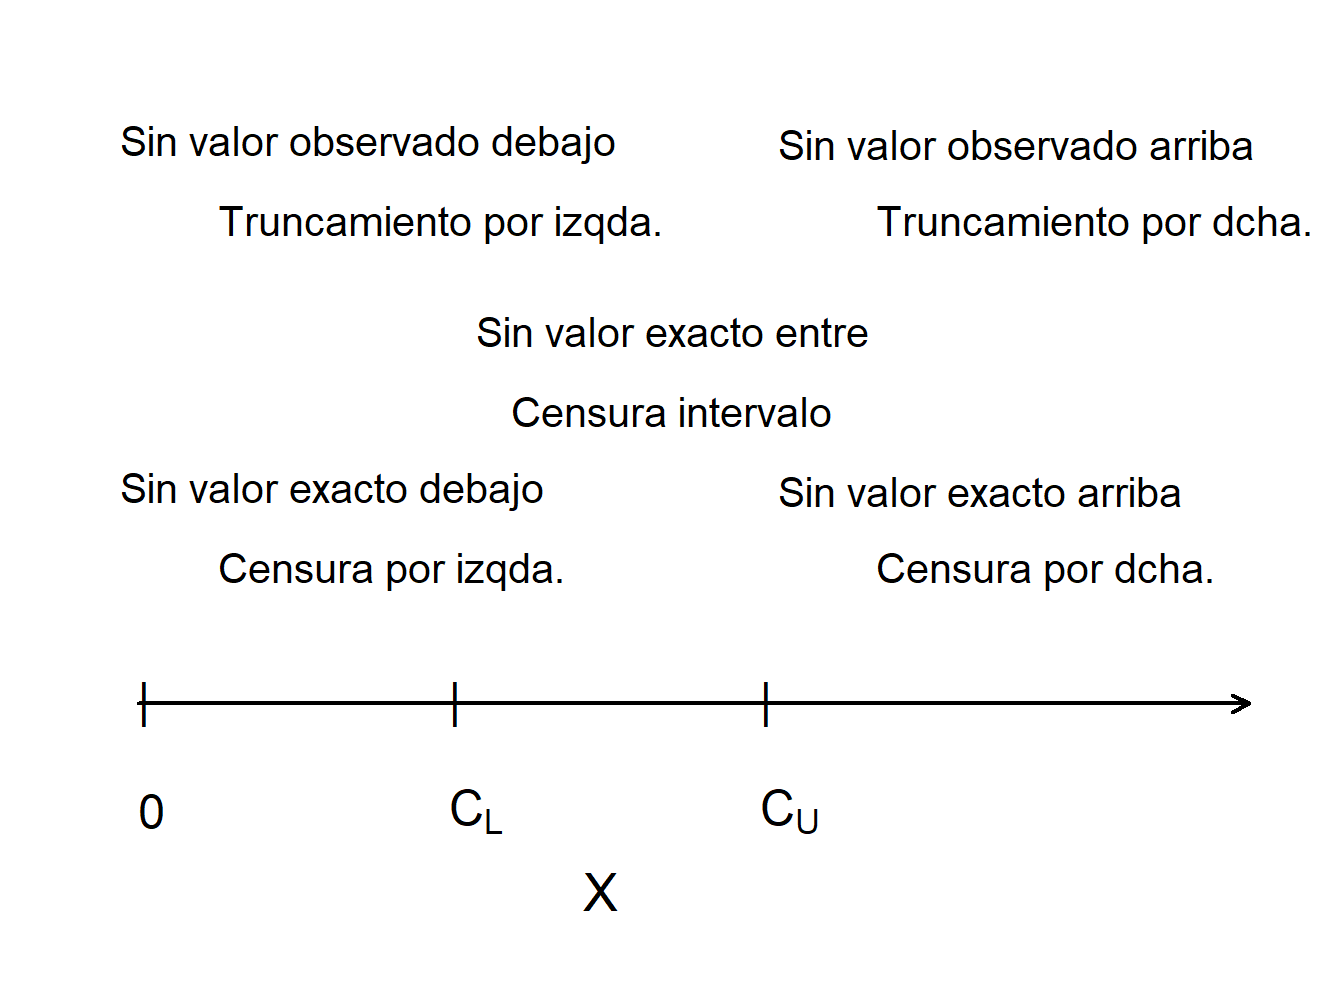
\includegraphics[width=0.6\linewidth]{LossDataAnalytics_files/figure-latex/CensorTrunc-1} 

}

\caption{Censura y Truncamiento}\label{fig:CensorTrunc}
\end{figure}

\begin{center}\rule{0.5\linewidth}{0.5pt}\end{center}

Mostrar ejemplo de estudio de mortalidad

\leavevmode\hypertarget{toggleExampleMort}{}%
\textbf{Ejemplo: estudio de mortalidad.} Supongamos que se está realizando un estudio de dos años de mortalidad de sujetos de alto riesgo, comenzando el 1 de enero de 2010 y terminando el 1 de enero de 2012. Figura \ref{fig:Mortality} representa gráficamente los seis tipos de sujetos reclutados. Para cada sujeto, el comienzo de la flecha representa que el sujeto fue reclutado y el final de la flecha representa el tiempo del evento. Por lo tanto, la flecha representa el tiempo de exposición.

\begin{figure}

{\centering 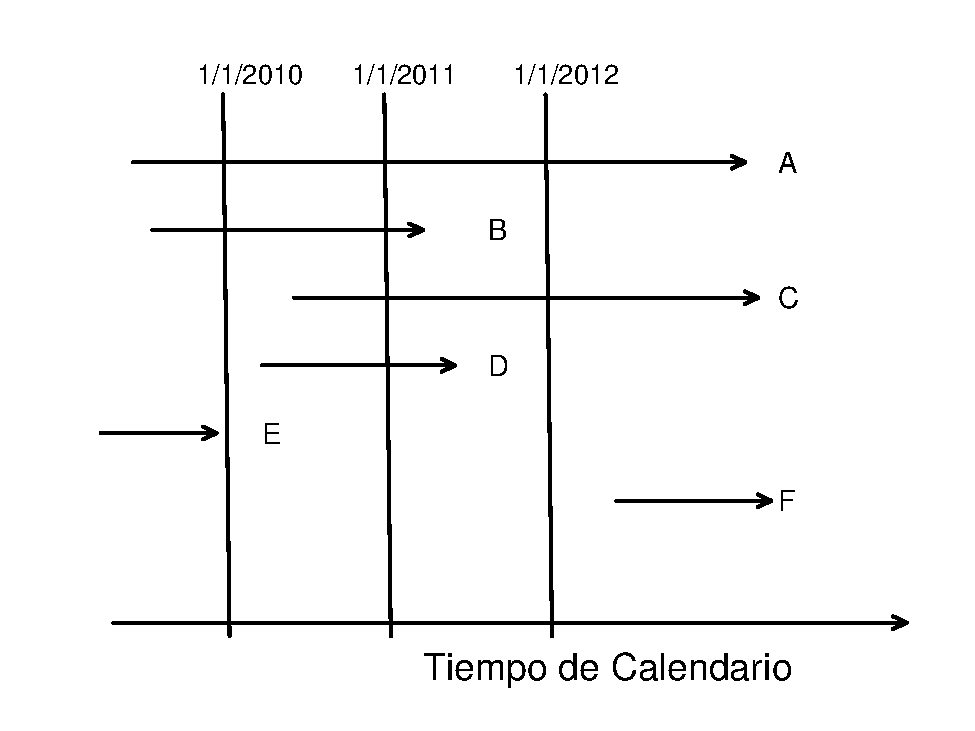
\includegraphics[width=0.6\linewidth]{LossDataAnalytics_files/figure-latex/Mortality-1} 

}

\caption{Cronología de varios sujetos en prueba en un estudio de mortalidad}\label{fig:Mortality}
\end{figure}

\begin{itemize}
\tightlist
\item
  \textbf{Tipo A: Censurado por la derecha. }Este sujeto está vivo al principio y al final del estudio. Debido a que no se conoce el momento de la muerte al final del estudio, está censurado correctamente. La mayoría de los sujetos son de tipo A.
\item
  \textbf{Tipo B- Información completa} está disponible para un sujeto tipo B. El sujeto está vivo al comienzo del estudio y la muerte ocurre dentro del período de observación.
\item
  \textbf{Tipo C: Censurado por la derecha y truncado a la izquierda.} Un sujeto de tipo C está censurado por la derecha, ya que la muerte ocurre después del período de observación. Sin embargo, el sujeto ingresó después del inicio del estudio y se dice que tiene un \emph{tiempo de entrada retrasado}. Debido a que el sujeto no habría sido observado si la muerte hubiera ocurrido antes de la entrada, se trunca a la izquierda.
\item
  \textbf{Tipo D: truncado por la izquierda.} Un sujeto de tipo D también ha retrasado la entrada. Debido a que la muerte ocurre dentro del período de observación, este individuo no está censurado a la derecha.
\item
  \textbf{Tipo E: truncado por la izquierda.} Un sujeto tipo E no está incluido en el estudio porque la muerte ocurre antes del período de observación.
\item
  \textbf{Tipo F: truncado por la derecha.} Del mismo modo, un sujeto tipo F no está incluido porque el tiempo de entrada ocurre después del período de observación.
\end{itemize}

\begin{center}\rule{0.5\linewidth}{0.5pt}\end{center}

Para resumir, para el resultado \(X\) y las constantes \(C_L\) y \(C_U\),

\begin{longtable}[]{@{}rcc@{}}
\toprule
Tipo de Limitación & Variable Limitada & Registro de Información \\
\midrule
\endhead
Censura por drcha. & \(X_U^{\ast}= \min(X,C_U)\) & \(\delta_U= I(X \leq C_U)\) \\
Censura por izda. & \(X_L^{\ast}= \max(X,C_L)\) & \(\delta_L= I(X \geq C_L)\) \\
Censura por intervalo & & \\
Truncamiento drcha. & \(X\) & observa \(X\) si \(X \leq C_U\) \\
Truncamiento izda. & \(X\) & observa \(X\) si \(X \geq C_L\) \\
\bottomrule
\end{longtable}

\hypertarget{estimaciuxf3n-paramuxe9trica-utilizando-datos-censurados-y-truncados}{%
\subsubsection{Estimación paramétrica utilizando datos censurados y truncados}\label{estimaciuxf3n-paramuxe9trica-utilizando-datos-censurados-y-truncados}}

Para simplificar, asumimos valores de censura no aleatorios y una variable continua \(X\). Empezamos considerando el caso de datos censurados a la derecha donde registramos \(X_U^{\ast}=\min(X,C_U)\) y el indicador de censura \(\delta=I(X \leq C_U)\). Si la censura ocurre, de modo que \(\delta = 0\), entonces \(X\geq C_U\) y la probabilidad es \(\Pr(X \geq C_U)=1-F(C_U)\). Si la censura no ocurre, de modo que \(\delta=1\), entonces \(X<C_U\) y la verosimilitud es \(f(x)\). Resumiendo, tenemos la verosimilitud de una sola observación como

\[
\begin{aligned}
\left\{
\begin{array}{ll}
1-F(C_U) & \text{if }\delta=0 \\
f(x) & \text{if } \delta = 1 
\end{array}
\right. = \left\{ f(x)\right\}^{\delta} \left\{1-F(C_U)\right\}^{1-\delta} .
\end{aligned}
\]

La expresión de a la derecha nos permite presentar la verosimilitud de manera más compacta. Ahora, para una muestra \emph{iid} de tamaño \(n\), la verosimilitud es

\[
\mathcal{L} = 
\prod_{i=1}^n \left\{ f(x_i)\right\}^{\delta_i} \left\{1-F(C_{Ui})\right\}^{1-\delta_i} = \prod_{\delta_i=1} f(x_i) \prod_{\delta_i=0} \{1-F(C_{Ui})\},
\]

con tiempos de censura potenciales \(\{C_{U1},\ldots, C_{Un} \}\). Aquí, la notación ``\(\prod_{\delta_i=1}\)'' significa el producto de las observaciones sin censura, y de manera similar para ``\(\prod_{\delta_i=0}\)''.

Por otro lado, los datos truncados se tratan en inferencia de verosimilitud mediante probabilidades condicionadas. En concreto, ajustamos la contribución a la verosimilitud dividiendo por la probabilidad de que se haya observado la variable. En resumen, tenemos las siguientes contribuciones a la función de verosimilitud para seis tipos de resultados:
\[
{\small
\begin{array}{lc}
\hline
\text{Resultado} & \text{Contribución en la Verosimilitud} \\
\hline
\text{Valor exacto} & f(x) \\
\text{Censura por la derecha} & 1-F(C_U) \\
\text{Censura por la izquierda} & F(C_L) \\
\text{Truncamiento por la derecha} & f(x)/F(C_U) \\
\text{Truncamiento por la izquierda} & f(x)/(1-F(C_L)) \\
\text{Censura por intervalo } & F(C_U)-F(C_L) \\
\hline
\end{array}
}
\]

Para resultados conocidos y datos censurados, la verosimilitud es
\[\mathcal{L}(\theta) = \prod_{E} f(x_i) \prod_{R} \{1-F(C_{Ui})\} \prod_{L}
F(C_{Li}) \prod_{I} (F(C_{Ui})-F(C_{Li})),\]
donde ``\(\prod_{E}\)'' es el producto sobre las observaciones con valores Exactos (\emph{E}), y de manera similar para los datos censurados por la Derecha (\emph{R}), Izquierda (\emph{L}) y en Intervalo (\emph{I}).

Para datos censurados por la derecha y truncados por la izquierda, la probabilidad es
\[\mathcal{L} = \prod_{E} \frac{f(x_i)}{1-F(C_{Li})} \prod_{R} \frac{1-F(C_{Ui})}{1-F(C_{Li})},\]
y de manera similar para otras combinaciones. Para obtener más información, considere lo siguiente.

\begin{center}\rule{0.5\linewidth}{0.5pt}\end{center}

Mostrar caso particular -- Distribución Exponencial

\leavevmode\hypertarget{toggleExampleEXP}{}%
\textbf{Caso especial: Distribución exponencial.} Considere los datos que están censurados por la derecha y truncados por la izquierda, con variables aleatorias \(X_i\) que se distribuyen exponencialmente con media \(\theta\). Con estas especificaciones, recuerde que \(f(x) = \theta^{-1} \exp(-x/\theta)\) y \(F(x) = 1-\exp(-x/\theta)\).

Para este caso particular, la log verosimilitud es

\[
\begin{aligned}
L(\theta) &= \sum_{E} \left\{ \ln f(x_i) - \ln (1-F(C_{Li})) \right\} + \sum_{R}\left\{ \ln (1-F(C_{Ui}))- \ln (1-\mathrm{F}(C_{Li})) \right\}\\
&= \sum_{E} (-\ln \theta -(x_i-C_{Li})/\theta ) -\sum_{R} (C_{Ui}-C_{Li})/\theta .
\end{aligned}
\]

Para simplificar la notación, definimos \(\delta_i=I(X_i\geq C_{Ui})\) como una variable binaria que indica la censura a la derecha. Sea \(X_i^{\ast\ast} = \min(X_i,C_{Ui})-C_{Li}\) la cantidad que la variable observada excede el límite inferior de truncamiento. Con esto, la log verosimilitud es

\begin{equation}
  L(\theta) =  - \sum_{i=1}^n ((1-\delta_i) \ln \theta + \frac{x_i^{\ast \ast}}{\theta}).
  \label{eq:EXPloglik}
\end{equation}

Derivando con respecto al parámetro \(\theta\) e igualando a cero se obtiene el estimador de máxima verosimilitud
\[\widehat{\theta}  = \frac{1}{n_u} \sum_{i=1}^n  x_i^{\ast \ast},\]

donde \(n_u = \sum_i (1-\delta_i)\) es el número de datos no censurados.

\begin{center}\rule{0.5\linewidth}{0.5pt}\end{center}

\textbf{Ejemplo 4.3.2. Pregunta de Examen Actuarial.}
Te dan:

\begin{enumerate}
\def\labelenumi{(\roman{enumi})}
\tightlist
\item
  Una muestra de pérdidas es: 600 700 900
\item
  No hay información disponible sobre pérdidas de 500 o menos.
\item
  Se supone que las pérdidas siguen una distribución exponencial con media \(\theta\).
\end{enumerate}

Calcular el estimador de máxima verosimilitud de \(\theta\).

Mostrar solución del ejemplo

\leavevmode\hypertarget{toggleExampleSelect.3.2}{}%
\textbf{Solución.}
Estas observaciones se truncan en 500. La contribución de cada observación a la función de verosimilitud es
\[\frac{f(x)}{1-F(500)} = \frac{\theta^{-1}e^{-x/\theta}}{e^{-500/\theta}}\]

Entonces la función de verosimilitud es

\[\mathcal{L}(\theta)= \frac{\theta^{-1} e^{-600/\theta} \theta^{-1} e^{-700/\theta} \theta^{-1} e^{-900/\theta}}{(e^{-500/\theta})^3} = \theta^{-3}e^{-700/\theta}\]

El logaritmo de la verosimilitud es

\[L(\theta) = \ln\mathcal{L}(\theta) = -3\ln \theta - 700\theta^{-1}\]

Maximizando esta expresión, estableciendo la derivada con respecto a \(\theta\) igual a 0, tenemos

\[L'(\theta) = -3\theta^{-1} + 700\theta^{-2} = 0 \ \Rightarrow \ \hat{\theta} = \frac{700}{3} = 233,33\]

\begin{center}\rule{0.5\linewidth}{0.5pt}\end{center}

\textbf{Ejemplo 4.3.3. Pregunta de Examen Actuarial.}
Se le proporciona la siguiente información sobre una muestra aleatoria:

\begin{enumerate}
\def\labelenumi{(\roman{enumi})}
\tightlist
\item
  El tamaño de la muestra es igual a cinco.
\item
  La muestra es de una distribución de Weibull con \(\tau = 2\).
\item
  Se sabe que dos de las observaciones de la muestra exceden 50, y las tres observaciones restantes son 20, 30 y 45.
\end{enumerate}

Calcule el estimador de máxima verosimilitud de \(\theta\).

Mostrar solución del ejemplo

\leavevmode\hypertarget{toggleExampleSelect.3.3}{}%
\textbf{Solución.} La función de verosimilitud es

\[
\begin{aligned} 
\mathcal{L}(\theta) &= f(20) f(30) f(45) [1-F(50)]^2 \\
&= \frac{2(20/\theta)^2 e^{-(20/\theta)^2}}{20} \frac{2(30/\theta)^2 e^{-(30/\theta)^2}}{30} \frac{2(45/\theta)^2 e^{-(45/\theta)^2}}{45}(e^{-(50/\theta)^2})^2 \\
&\propto \frac{1}{\theta^6} e^{-8325/\theta^2}
\end{aligned}
\]

El logaritmo natural de la expresión anterior es \(-6\ln\theta-\frac{8325}{\theta^2}\). Maximizando esta expresión al fijar su derivada igual a 0, obtenemos

\[\frac{-6}{\theta} + \frac{16650}{\theta^3} = 0 \ \Rightarrow \ \hat{\theta} = \left(\frac{16650}{6}\right)^{\frac{1}{2}} = 52,6783\]

\begin{center}\rule{0.5\linewidth}{0.5pt}\end{center}

\hypertarget{estimaciuxf3n-no-paramuxe9trica-utilizando-datos-modificados}{%
\subsection{Estimación no Paramétrica Utilizando Datos Modificados}\label{estimaciuxf3n-no-paramuxe9trica-utilizando-datos-modificados}}

Los estimadores no paramétricos proporcionan puntos de referencia útiles, por lo que es útil comprender los procedimientos de estimación para datos agrupados, censurados y truncados.

\hypertarget{datos-agrupados}{%
\subsubsection{Datos Agrupados}\label{datos-agrupados}}

Como hemos visto en la Sección \ref{S:MS:GroupedData}, las observaciones pueden agruparse (también denominadas censuradas por intervalos) en el sentido de que solo las observamos como pertenecientes a uno de los \(k\) intervalos de la forma \((c_{j-1},c_j]\), para \(j=1,\ldots,k\). En los límites, la función de distribución empírica se define de la manera habitual:

\[
F_n(c_j) = \frac{\text{número de observaciones } \le c_j}{n}.
\]

Para otros valores de \(x \in (c_{j-1},c_j)\), podemos estimar la función de distribución con el estimador \emph{ogive}, que interpola linealmente entre \(F_n(c_{j-1})\) y \(F_n(c_j)\), es decir, los valores de los límites \(F_n(c_{j-1})\) y \(F_n (c_j)\) están conectados con una línea recta. Esto puede expresarse formalmente como
\[F_n(x) = \frac{c_j-x}{c_j-c_{j-1}} F_n(c_{j-1}) + \frac{x-c_{j-1}}{c_j-c_{j-1}} F_n(c_j) \ \ \ \text{para } c_{j-1} \le x < c_j\]

La densidad correspondiente es
\[f_n(x) = F^{\prime}_n(x) = \frac{F_n(c_j)-F_n(c_{j-1})}{c_j - c_{j-1}} \ \ \  \text{para } c_{j-1} \le x < c_j .\]

\begin{center}\rule{0.5\linewidth}{0.5pt}\end{center}

\textbf{Ejemplo 4.3.4. Pregunta de Examen Actuarial.}

Se le proporciona la siguiente información sobre los cantidades reclamadas para 100 siniestros:

\[
{\small
\begin{array}{r|c}
\hline
\text{Tamaño del Siniestro} &  \text{Número de Siniestros } \\
\hline
0 – 1.000 & 16 \\
1.000 – 3.000 & 22 \\
3.000 – 5.000 & 25 \\
5.000 – 10.000 & 18 \\
10.000 – 25.000 & 10 \\
25.000 – 50.000 & 5 \\
50.000 – 100.000 & 3 \\
\text{mayor  } 100.000 & 1 \\
\hline
\end{array}
}
\]

Usando el estimador \emph{ogive}, calcule la estimación de la probabilidad de que un siniestro elegido al azar esté entre 2000 y 6000.

Mostrar solución del ejemplo

\leavevmode\hypertarget{toggleExampleSelect.3.4}{}%
\textbf{Solución.}
En los límites, la función de distribución empírica se define de la manera habitual, por lo que tenemos
\[F_{100}(1000) = 0,16, \ F_{100}(3000)=0,38, \ F_{100}(5000)=0,63, \ F_{100}(10000)=0,81.\]
Para otros tamaños del siniestro, el estimador \emph{ogive} interpola linealmente entre estos valores:
\[F_{100}(2000) = 0,5F_{100}(1000) + 0,5F_{100}(3000) = 0,5(0,16)+0,5(0,38)=0,27\] \[F_{100}(6000)=0,8F_{100}(5000)+0,2F_{100}(10000) = 0,8(0,63)+0,2(0,81)=0,666\]
Por lo tanto, la probabilidad de que una reclamación esté entre 2000 y 6000 es \(F_{100}(6000) - F_{100}(2000) = 0,666-0,27 = 0,396\).

\begin{center}\rule{0.5\linewidth}{0.5pt}\end{center}

\hypertarget{funciuxf3n-de-distribuciuxf3n-empuxedrica-censurada-por-la-derecha}{%
\subsubsection{Función de Distribución Empírica Censurada por la Derecha}\label{funciuxf3n-de-distribuciuxf3n-empuxedrica-censurada-por-la-derecha}}

Puede ser útil calibrar los estimadores paramétricos con métodos no paramétricos que no se basen en una forma paramétrica de la distribución. El estimador de límite de producto propuesto por \citep{kaplan1958} es un estimador de la función de distribución bien conocido en presencia de censura.

\textbf{Motivación para el Estimador de Límite de Producto de Kaplan-Meier.} Para explicar por qué el límite de producto funciona tan bien con observaciones censuradas, volvamos primero al caso ``habitual'' sin censura. Aquí, la función de distribución empírica \(F_n(x)\) es un estimador \emph{insesgado} de la función de distribución \(F(x)\). Esto se debe a que \(F_n(x)\) es el promedio de las variables indicadoras, cada una de las cuales es insesgada, es decir, \(\mathrm{E~}I(X_i \le x) = \Pr(X_i \le x) = F(x)\).

Ahora supongamos que la variable aleatoria está censurada por la derecha por una cantidad límite, por ejemplo, \(C_U\), de modo que registramos el menor de los dos, \(X^* = \min(X, C_U)\). Para valores de \(x\) que son menores que \(C_U\), la variable indicadora todavía proporciona un estimador insesgado de la función de distribución antes de alcanzar el límite de censura. Es decir, \(\mathrm{E ~}I(X^* \le x) = F(x)\) porque \(I(X^* \le x) = I(X \le x)\) para \(x<C_U\). Del mismo modo, \(\mathrm{E~}I(X^*> x) = 1-F(x) = S(x)\). En cambio, para \(x>C_U\), \(I(X^* \le x)\) en general no es un estimador insesgado de \(F(x)\).

Como alternativa, consideremos \emph{dos} variables aleatorias que tienen diferentes límites de censura. Por ejemplo, supongamos que observamos \(X_1^* = \min(X_1, 5)\) y \(X_2^* = \min(X_2, 10)\), donde \(X_1\) y \(X_2\) son extracciones independientes de la misma distribución. Para \(x\le 5\), la función de distribución empírica \(F_2(x)\) es un estimador insesgado de \(F(x)\). Sin embargo, para \(5<x \le 10\), la primera observación no puede usarse para la función de distribución debido a la limitación de censura. En cambio, la estrategia desarrollada por \citep{kaplan1958} es usar \(S_2(5)\) como estimador de \(S(5)\) y luego usar la segunda observación para estimar la función de supervivencia condicional a la supervivencia al tiempo 5, \(\Pr(X>x|X>5) = \frac {S(x)}{S(5)}\). Específicamente, para \(5<x \le 10\), el estimador de la función de supervivencia es

\[
\hat{S}(x) = S_2(5) \times I(X_2^* > x ) .
\]

\textbf{Estimador del límite de producto de Kaplan-Meier.} Ampliando esta idea, para cada observación \(i\), sea \(u_i\) el límite superior de censura (\(= \infty\) si no hay censura). Por lo tanto, el valor registrado es \(x_i\) en el caso de no censura y \(u_i\) si hay censura. Supongamos que \(t_{1}<\cdots<t_{k}\) sean \(k\) puntos distintos en los que se produce una pérdida sin censura, y que \(s_j\) sea el número de pérdidas sin censura \(x_i\)'s en \(t_{j}\). El \textbf{conjunto de riesgo} correspondiente es el número de observaciones que están activas (no censuradas) en un valor \emph{menor que} \(t_{j}\), denotado como \(R_j=\sum_{i = 1}^n I(x_i \geq t_{j})+\sum_{i = 1}^n I(u_i \geq t_{j})\).

Con esta notación, el \textbf{estimador del límite de producto} de la función de distribución es
\begin{equation}
\hat{F}(x) =
\left\{
\begin{array}{ll}
0 & x<t_{1} \\
1-\prod_{j:t_{j} \leq x}\left( 1-\frac{s_j}{R_{j}}\right) & x \geq t_{1} 
\end{array}
\right. .\label{eq:KaplanMeier}
\end{equation}

Como de costumbre, la estimación correspondiente de la función de supervivencia es \(\hat{S}(x) = 1 - \hat{F}(x)\).

\begin{center}\rule{0.5\linewidth}{0.5pt}\end{center}

\textbf{Ejemplo 4.3.5. Pregunta de Examen Actuarial.}
La siguiente es una muestra de 10 pagos:

\[
\begin{array}{cccccccccc}
4 &4 &5+ &5+ &5+ &8 &10+ &10+ &12 &15 \\
\end{array}
\]

donde \(+\) indica que una pérdida ha excedido el límite de la póliza.

Usando el estimador de límite de producto de Kaplan-Meier, calcule la probabilidad de que la pérdida en una póliza exceda 11, \(\hat{S}(11)\).

Mostrar solución del ejemplo

\leavevmode\hypertarget{toggleExampleSelect.3.5}{}%
\textbf{Solución.}
Hay cuatro tiempos de eventos (observaciones no censuradas). Para cada tiempo \(t_j\), podemos calcular el número de eventos \(s_j\) y el conjunto de riesgo \(R_j\) de la siguiente manera:

\[
\begin{array}{cccc}
\hline
j & t_j & s_j & R_j \\
\hline
1 & 4 & 2 & 10 \\
2 & 8 & 1 & 5 \\
3 & 12 & 1 & 2 \\
4 & 15 & 1 & 1 \\
\hline
\end{array}
\]

Asi, la estimación de Kaplan-Meier de \(S(11)\) es
\[
\begin{aligned}
\hat{S}(11) &= \prod_{j:t_j\leq 11} \left( 1- \frac{s_j}{R_j} \right) =  \prod_{j=1}^{2} \left( 1- \frac{s_j}{R_j} \right)\\
&= \left(1-\frac{2}{10} \right) \left(1-\frac{1}{5} \right) = (0,8)(0,8)= 0,64. \\
\end{aligned}
\]

\begin{center}\rule{0.5\linewidth}{0.5pt}\end{center}

\textbf{Ejemplo. 4.3.6. Siniestros con Daños Corporales.} Consideramos nuevamente los datos de la aplicación de \citet{derrig2001applications} de siniestros por daños corporales en automóviles en Boston, que se presentaron en el Ejemplo 4.1.11. En ese ejemplo, omitimos los siniestros 17 que fueron censurados por los límites de la póliza. Ahora, incluimos el conjunto de datos completo y utilizamos el estimador del límite de producto de Kaplan-Meier para estimar la función de supervivencia. Esto se muestra en la Figura \ref{fig:KMSurvival}.

\begin{figure}

{\centering 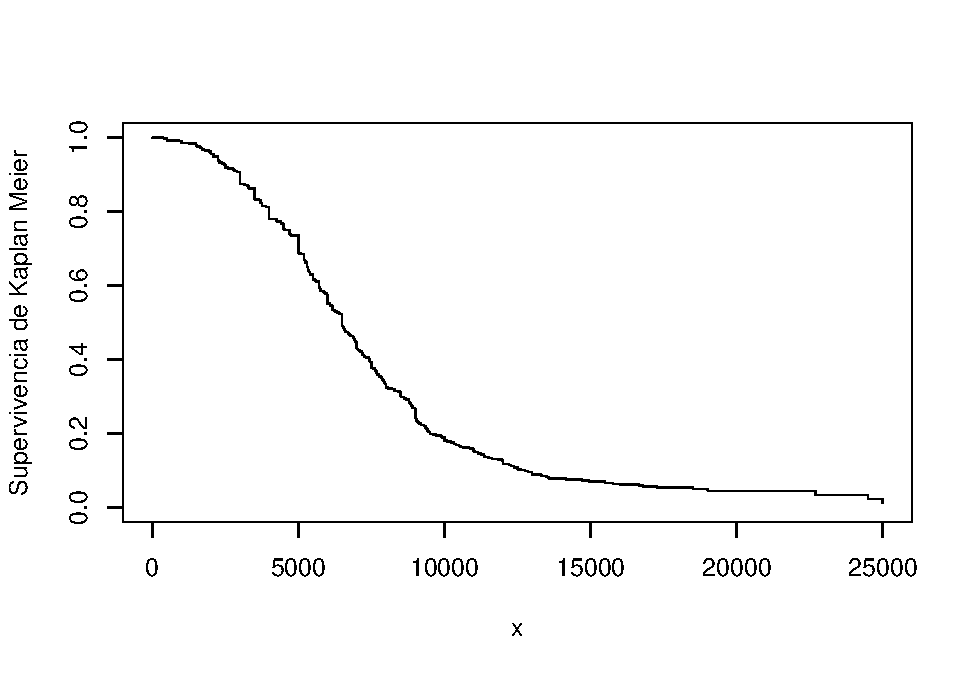
\includegraphics{LossDataAnalytics_files/figure-latex/KMSurvival-1} 

}

\caption{Estimación de Kaplan-Meier de la función de supervivencia para siniestros por daños corporales }\label{fig:KMSurvival}
\end{figure}

Mostrar código R

\hypertarget{toggleKaplanMeier}{}
\begin{Shaded}
\begin{Highlighting}[]
\FunctionTok{library}\NormalTok{(survival)                }\CommentTok{\# para Surv(), survfit()}
\DocumentationTok{\#\# KM estimación}
\NormalTok{KM0 }\OtherTok{\textless{}{-}} \FunctionTok{survfit}\NormalTok{(}\FunctionTok{Surv}\NormalTok{(AmountPaid, UnCensored) }\SpecialCharTok{\textasciitilde{}} \DecValTok{1}\NormalTok{,  }\AttributeTok{type=}\StringTok{"kaplan{-}meier"}\NormalTok{, }\AttributeTok{data=}\NormalTok{BIData)}
\FunctionTok{plot}\NormalTok{(KM0, }\AttributeTok{conf.int=}\ConstantTok{FALSE}\NormalTok{, }\AttributeTok{xlab=}\StringTok{"x"}\NormalTok{,}\AttributeTok{ylab=}\StringTok{"Supervivencia de Kaplan Meier "}\NormalTok{)}
\end{Highlighting}
\end{Shaded}

\begin{center}\rule{0.5\linewidth}{0.5pt}\end{center}

\hypertarget{funciuxf3n-de-distribuciuxf3n-empuxedrica-censurada-por-la-derecha-truncada-por-la-izquierda}{%
\subsubsection{Función de Distribución Empírica Censurada por la Derecha, Truncada por la Izquierda}\label{funciuxf3n-de-distribuciuxf3n-empuxedrica-censurada-por-la-derecha-truncada-por-la-izquierda}}

Además de la censura por la derecha, ahora ampliamos el marco para permitir datos truncados por la izquierda. Como antes, para cada observación \(i\), sea \(u_i\) el límite superior de censura (\(= \infty\) si no hay censura). Además, sea \(d_i\) el límite inferior de truncamiento (0 si no hay truncamiento). Por lo tanto, el valor registrado (si es mayor que \(d_i\)) es \(x_i\) en el caso de no censura y \(u_i\) si hay censura. Supongamos que \(t_{1} <\cdots <t_{k}\) son \(k\) puntos distintos en los que se produce un evento de interés, y que \(s_j\) son el número de eventos registrados \(x_i\)'s en el punto de tiempo \(t_{j}\). El conjunto de riesgos correspondiente es
\[R_j = \sum_{i=1}^n I(x_i \geq t_{j}) + \sum_{i=1}^n I(u_i \geq t_{j}) - \sum_{i=1}^n I(d_i \geq t_{j}).\]

Con esta nueva definición del conjunto de riesgos, el estimador del límite de producto de la función de distribución es como en la ecuación \eqref{eq:KaplanMeier}.

\textbf{Fórmula de Greenwood}. \citep{greenwood1926} obtuvo la fórmula para que la varianza estimada del estimador de límite de producto sea
\[\widehat{Var}(\hat{F}(x)) = (1-\hat{F}(x))^{2} \sum _{j:t_{j} \leq x} \dfrac{s_j}{R_{j}(R_{j}-s_j)}.\]

El método de \texttt{R} \texttt{survfit} utiliza un objeto de datos de supervivencia y crea un nuevo objeto que contiene la estimación de Kaplan-Meier de la función de supervivencia junto con los intervalos de confianza. El método de Kaplan-Meier (\texttt{type\ =\ \textquotesingle{}kaplan-meier\textquotesingle{}}) se usa por defecto para construir una estimación de la curva de supervivencia. La función de supervivencia discreta resultante tiene puntos de masa en los tiempos de evento observados (fechas de alta) \(t_j\), donde la probabilidad de supervivencia de un evento a esa duración se estima como el número de eventos observados en la duración \(s_j\) dividido por el número de sujetos expuestos o `en riesgo' justo antes de la duración del evento \(R_j\).

Dos tipos alternativos de estimación también están disponibles para el método \texttt{survfit}. La alternativa (\texttt{type=\textquotesingle{}fh2\textquotesingle{}}) maneja los empates, en esencia, al suponer que ocurren varios eventos con la misma duración en un orden arbitrario. Otra alternativa (\texttt{type=\textquotesingle{}fleming-harrington\textquotesingle{}}) usa el estimador de Nelson-Aalen (see \citep{aalen1978}) en la estimación de la \textbf{función de riesgo (hazard) acumulado} para obtener una estimación de la función de supervivencia. El riesgo acumulado estimado \(\hat{H}(x)\) comienza en cero y se incrementa en cada evento observado de duración \(t_j\) por el número de eventos \(s_j\) dividido por el número en riesgo \(R_j\). Con la misma notación anterior, el estimador de \textbf{Nelson-Aalen} de la función de distribución es

\[
\begin{aligned}
\hat{F}_{NA}(x) &=
\left\{
\begin{array}{ll}
0 & x<t_{1} \\
1- \exp \left(-\sum_{j:t_{j} \leq x}\frac{s_j}{R_j} \right) & x \geq t_{1} 
\end{array}
\right. .\end{aligned}
\]

Cabe tener en cuenta que la expresión anterior es el resultado del estimador de Nelson-Aalen de la función de riesgo acumulado
\[\hat{H}(x) = \sum_{j: t_j \leq x}\frac{s_j}{R_j}\]
y la relación entre la función de supervivencia y la función de riesgo acumulado es \(\hat{S}_{NA}(x) = e^{-\hat{H}(x)}\).

\begin{center}\rule{0.5\linewidth}{0.5pt}\end{center}

\textbf{Ejemplo 4.3.7. Pregunta de Examen Actuarial.}

Para la observación \(i\) de un estudio de supervivencia:

\begin{itemize}
\tightlist
\item
  \(d_i\) es el punto de truncamiento a la izquierda
\item
  \(x_i\) es el valor observado si no está censurado a la derecha
\item
  \(u_i\) es el valor observado si se censura a la derecha
\end{itemize}

Te dan:

\[
{\small
\begin{array}{c|cccccccccc}
\hline
\text{Observación } (i) & 1 & 2 & 3 & 4 & 5 & 6 & 7 & 8 & 9 & 10\\ \hline
d_i & 0 & 0 & 0 & 0 & 0 & 0 & 0 & 1,3 & 1,5 & 1,6\\
x_i & 0,9 & - & 1,5 & - & - & 1,7 & - & 2,1 & 2,1 & - \\
u_i & - & 1,2 & - & 1,5 & 1,6 & - & 1,7 & - & - & 2,3 \\
\hline
\end{array}
}
\]

Calcular la estimación del límite de producto de Kaplan-Meier, \(\hat{S}(1,6)\)

Mostrar solución del ejemplo

\leavevmode\hypertarget{toggleExampleSelect.3.6}{}%
\textbf{Solución.} Recordemos el conjunto de riesgo \(R_j = \sum_{i=1}^n \left\{ I(x_i \geq t_{j}) + I(u_i \geq t_{j}) - I(d_i \geq t_{j}) \right\}\). Entonces

\[
\begin{array}{ccccc}
\hline
j & t_j & s_j & R_j & \hat{S}(t_j) \\
\hline
1  & 0,9   & 1   & 10-3 = 7 & 1-\frac{1}{7} = \frac{6}{7} \\
2  & 1,5   & 1   & 8-2 = 6  & \frac{6}{7}\left( 1 - \frac{1}{6} \right) = \frac{5}{7}\\
3  & 1,7   & 1   & 5-0 = 5  & \frac{5}{7}\left( 1 - \frac{1}{5} \right) = \frac{4}{7}\\
4  & 2,1   & 2   & 3        & \frac{4}{7}\left( 1 - \frac{2}{3}\right) = \frac{4}{21}\\
\hline
\end{array}
\]

La estimación de Kaplan-Meier es por lo tanto \(\hat{S}(1,6) = \frac{5}{7}\).

\begin{center}\rule{0.5\linewidth}{0.5pt}\end{center}

\textbf{Ejemplo 4.3.8. Pregunta de Examen Actuarial. -- Continuación.}

\begin{enumerate}
\def\labelenumi{\alph{enumi})}
\tightlist
\item
  Usando el estimador de Nelson-Aalen, calcular la probabilidad de que la pérdida en una póliza exceda 11, \(\hat{S}_{NA}(11)\).
\item
  Calcular la aproximación de Greenwood de la varianza de la estimación del límite del producto \(\hat{S}(11)\).
\end{enumerate}

Mostrar solución del ejemplo

\leavevmode\hypertarget{toggleExampleSelect.3.7}{}%
\textbf{Solución.}
Como antes, hay cuatro tiempos con eventos (observaciones no censuradas). Para cada tiempo \(t_j\) podemos calcular el número de eventos \(s_j\) y el conjunto de riesgo \(R_j\) de la siguiente manera:
\[
\begin{array}{cccc}
\hline
j & t_j & s_j & R_j \\
\hline
1 & 4 & 2 & 10 \\
2 & 8 & 1 & 5 \\
3 & 12 & 1 & 2 \\
4 & 15 & 1 & 1 \\
\hline
\end{array}
\]

El estimador de Nelson-Aalen de \(S(11)\) es \(\hat{S}_{NA}(11)=e^{-\hat{H}(11)} = e^{-0,4} = 0,67\), de modo que
\[
\begin{aligned}
\hat{H}(11) &= \sum_{j:t_j\leq 11} \frac{s_j}{R_j}  = \sum_{j=1}^{2} \frac{s_j}{R_j}  \\
&= \frac{2}{10} + \frac{1}{5}  = 0,2 + 0,2 = 0,4 .\\
\end{aligned}
\]
Del ejercicio anterior, la estimación de Kaplan-Meier de \(S(11)\) es \(\hat{S}(11) = 0,64\). Entonces, la estimación de Greenwood de la varianza de la estimación del límite del producto de \(S(11)\) es
\[
\begin{aligned}
\widehat{Var}(\hat{S}(11)) &= (\hat{S}(11))^2 \sum_{j:t_j\leq 11} \frac{s_j}{R_j(R_j-s_j)}
&= (0,64)^2 \left(\frac{2}{10(8)} + \frac{1}{5(4)} \right)  = 0,0307. \\
\end{aligned}
\]

\begin{center}\rule{0.5\linewidth}{0.5pt}\end{center}

\hypertarget{S:MS:BayesInference}{%
\section{Inferencia Bayesiana}\label{S:MS:BayesInference}}

\begin{center}\rule{0.5\linewidth}{0.5pt}\end{center}

En esta sección aprende a:

\begin{itemize}
\tightlist
\item
  Describir el modelo bayesiano como una alternativa al enfoque frecuentista y resumir los cinco componentes de este enfoque de modelización.
\item
  Describir las distribuciones a posteriori de los parámetros y utilizar estas distribuciones para predecir nuevos resultados.
\item
  Utilizar distribuciones conjugadas para determinar las distribuciones a posteriori de los parámetros.
\end{itemize}

\begin{center}\rule{0.5\linewidth}{0.5pt}\end{center}

\hypertarget{S:IntroBayes}{%
\subsection{Introducción a la Inferencia Bayesiana}\label{S:IntroBayes}}

Hasta este punto, nuestros métodos inferenciales se han centrado en el entorno \textbf{frecuentista}, en el que se extraen muestras repetidamente de una población. El vector de parámetros \(\boldsymbol \theta\) es fijo pero desconocido, mientras que los resultados \(X\) son realizaciones procedentes de variables aleatorias.

En contraste, bajo el marco \textbf{Bayesiano}, consideramos los parámetros del modelo y los datos como variables aleatorias. No estamos seguros de los valores de los parámetros \(\boldsymbol \theta\) y utilizamos herramientas de probabilidad para reflejar esta incertidumbre.

Para tener una idea del marco bayesiano, recordemos primero la regla de Bayes
\[
\Pr(parámetros|datos) = \frac{\Pr(datos|parámetros) \times \Pr(parámetros)}{\Pr(datos)}
\]

donde

\begin{itemize}
\tightlist
\item
  \(\Pr(parámetros)\) es la distribución de los parámetros, conocida como la distribución \emph{a priori}.
\item
  \(\Pr(datos|parámetros)\) es la distribución de muestreo. En un contexto frecuentista, se usa para realizar inferencias sobre los parámetros y se conoce como \emph{probabilidad}.
\item
  \(\Pr(parámetros|datos)\) es la distribución de los parámetros que han observado los datos, conocidos como la distribución \emph{a posteriori}.
\item
  \(\Pr(datos)\) es la distribución marginal de los datos. Generalmente se obtiene integrando (o sumando) la distribución conjunta de datos y parámetros sobre los valores de los parámetros.
\end{itemize}

\textbf{¿Por qué Bayes?} Hay varias ventajas del enfoque bayesiano. Primero, podemos describir la distribución completa de parámetros condicionada a los datos. Esto nos permite, por ejemplo, proporcionar resultados de probabilidad con respecto a la verosimilitud de los parámetros. En segundo lugar, el enfoque bayesiano proporciona una alternativa unificada para estimar parámetros. Algunos métodos no bayesianos, como los mínimos cuadrados, requieren un enfoque separado para estimar los componentes de la varianza. Por el contrario, en los métodos bayesianos, todos los parámetros se pueden tratar de manera similar. Esto es conveniente para explicar los resultados a los usuarios del análisis de datos. Tercero, este enfoque permite a los analistas combinar información previa conocida de otras fuentes con los datos de manera coherente. Este tema se desarrolla en detalle en el capítulo de credibilidad. Cuarto, el análisis bayesiano es particularmente útil para pronosticar respuestas futuras.

\textbf{Caso particular de Poisson - Gamma.} Para desarrollar el método bayesiano de forma intuitiva, consideramos el caso de Poisson-Gamma que ocupa un lugar destacado en las aplicaciones actuariales. La idea es considerar un conjunto de variables aleatorias \(X_1,\ldots, X_n\), donde cada \(X_i\) podría representar el número de siniestros para el titular de la póliza \emph{i}-ésima. Supongamos que \(X_i\) tiene una distribución de Poisson con parámetro \(\lambda\), análoga a la probabilidad que vimos por primera vez en el Capítulo \ref{C:Frequency-Modeling}. En un contexto no bayesiano (o frecuentista), el parámetro \(\lambda\) se ve como una cantidad desconocida que no es aleatoria (se dice que es ``fija''). En el contexto bayesiano, el parámetro desconocido \(\lambda\) se considera incierto y se modeliza como una variable aleatoria. En este caso particular, utilizamos la distribución gamma para reflejar esta incertidumbre, la distribución a priori.

Pensemos en el siguiente esquema de muestreo en dos etapas para argumentar esta configuración probabilística.

\begin{enumerate}
\def\labelenumi{\arabic{enumi}.}
\tightlist
\item
  En la primera etapa, el parámetro \(\lambda\) se extrae de una distribución gamma.
\item
  En la segunda etapa, para ese valor de \(\lambda\), hay \(n\) extracciones de la misma distribución de Poisson, que son independientes, condicionadas a \(\lambda\).
\end{enumerate}

De esta configuración sencilla, surgen algunas conclusiones importantes.

\begin{itemize}
\tightlist
\item
  La distribución de \(X_i\) ya no es Poisson. Para el caso particular, es una distribución binomial negativa (ver el siguiente ``Fragmento de teoría'').
\item
  Las variables aleatorias \(X_1, \ldots, X_n\) no son independientes. Esto se debe a que comparten la variable aleatoria común \(\lambda\).
\item
  Como en el contexto frecuentista, el objetivo es hacer afirmaciones sobre los valores probables de los parámetros, tales como \(\lambda\), dado los datos observados \(X_1, \ldots, X_n\). Sin embargo, debido a que ahora tanto el parámetro como los datos son variables aleatorias, podemos usar el lenguaje de probabilidad condicionada para hacer tales afirmaciones. Como veremos en la Sección \ref{S:ConjugateDistributions}, resulta que la distribución de \(\lambda\) dados los datos \(X_1, \ldots, X_n\) también es gamma (con parámetros actualizados), un resultado que simplifica la tarea de inferir valores probables del parámetro \(\lambda\).
\end{itemize}

Mostrar un fragmento de teoría

\hypertarget{TheoryBayesPoisson}{}
\begin{center}\rule{0.5\linewidth}{0.5pt}\end{center}

Demostremos que la distribución de \(X\) es binomial negativa. Suponemos que la distribución de \(X\) dada \(\lambda\) es Poisson, de modo que
\[
\Pr(X = x|\lambda) = \frac{\lambda^x}{\Gamma(x+1)} e^{-\lambda} ,
\]
usando la notación \(\Gamma(x+1) = x!\) para el entero \(x\). Suponga que \(\lambda\) es una extracción de una distribución gamma con parámetros fijos, por ejemplo, \(\alpha\) y \(\theta\), por lo que esto tiene \emph{pdf}{ función de probabilidad de densidad}
\[
f(\lambda) = \frac{\lambda^{\alpha-1}}{\theta^{\alpha}\Gamma(\alpha)}\exp(-\lambda/\theta).
\]
Sabemos que una \emph{pdf} integra uno. Para facilitar el desarrollo, definimos el parámetro recíproco \(\theta_r = 1/\theta\) y así tenemos
\[
\int_0^{\infty} f(\lambda) ~d\lambda =1 ~~~ ==> ~~~ \theta_r^{-\alpha} \Gamma(\alpha) = \int_0^{\infty} \lambda^{\alpha-1} \exp\left(-\lambda\theta_r\right) ~
d\lambda .
\]
A partir del Capítulo de Apéndice \ref{C:AppB} en esperanzas iteradas, tenemos que la \emph{pmf}{ función masa de probabilidad} de \(X\) se puede calcular de forma iterada como

\[
\begin{aligned}
\Pr(X = x) 
&=  \mathrm{E} \left\{\Pr(X = x|\lambda)\right\}\\
&=  \int_0^{\infty} \Pr(X = x|\lambda) f(\lambda) ~d\lambda \\
&=  \int_0^{\infty} \frac{\lambda^x}{\Gamma(x+1)} e^{-\lambda} \frac{\lambda^{\alpha-1}}{\theta^{\alpha}\Gamma(\alpha)}\exp(-\lambda/\theta) ~d\lambda\\
&=  \frac{1}{\theta^{\alpha}\Gamma(x+1)\Gamma(\alpha)} \int_0^{\infty} \lambda^{x+\alpha-1} \exp\left(-\lambda(1+\frac{1}{\theta})\right) ~d\lambda \\
&=  \frac{1}{\theta^{\alpha}\Gamma(x+1)\Gamma(\alpha)} \Gamma(x+\alpha)\left(1+\frac{1}{\theta}\right)^{-(x+\alpha)} \\
&=  \frac{\Gamma(x+\alpha)}{\Gamma(x+1)\Gamma(\alpha)}\left(\frac{1}{1+\theta}\right)^{\alpha} \left(\frac{\theta}{1+\theta}\right)^{x} .\\
\end{aligned} 
\]
Aquí, utilizamos la igualdad de distribución gamma con la sustitución \(\theta_r = 1+1/\theta\). Como se puede ver en la Sección\ref{S:negative-binomial-distribution}, ésta es una distribución binomial negativa con parámetro \(r = \alpha\) y \(\beta = \theta\).

\begin{center}\rule{0.5\linewidth}{0.5pt}\end{center}

En este capítulo, usamos ejemplos sencillos que se pueden hacer a mano para ilustrar los fundamentos. Para una implementación práctica, los analistas dependen en gran medida de los métodos de simulación que utilizan métodos computacionales modernos como la simulación Markov Chain Monte Carlo (\emph{MCMC}). Realizaremos una introducción a las técnicas de simulación en el Capítulo \ref{C:Simulation}, pero las técnicas más intensivas como \emph{MCMC} requieren referencias adicionales. Ver @ hartman2016 para una introducción a los métodos bayesianos computacionales desde una perspectiva actuarial.

\hypertarget{modelo-bayesiano}{%
\subsection{Modelo Bayesiano}\label{modelo-bayesiano}}

Con el desarrollo intuitivo de la Sección anterior \ref{S:IntroBayes}, ahora reformulamos el modelo bayesiano con un poco más de precisión utilizando la notación matemática. Para simplificar, este resumen supone que tanto los resultados como los parámetros son variables aleatorias continuas. En los ejemplos, a veces le pedimos al lector que aplique estos mismos principios a versiones discretas. Conceptualmente, tanto los casos continuos como los discretos son iguales; mecánicamente, uno reemplaza un\emph{pdf}{ función de densidad de probabilidad} por una \emph{pmf}{ función masa de probabilidad} y una integral por una suma.

Como se indicó anteriormente, bajo la perspectiva bayesiana, los parámetros y los datos del modelo se consideran aleatorios. Nuestra incertidumbre sobre los parámetros del proceso subyacente de generación de datos se refleja en el uso de herramientas de probabilidad.

\textbf{Distribución A Priori.}
En concreto, pensemos en los parámetros \(\boldsymbol \theta\) como un vector aleatorio y denotemos \(\pi(\boldsymbol \theta)\) a la distribución de posibles resultados. Éste es el conocimiento que tenemos antes de que se observen los resultados y se denomina distribución a priori. Por lo general, la distribución a priori es una distribución regular y, por lo tanto, se integra o suma uno, dependiendo de si \(\boldsymbol \theta\) es continuo o discreto. Sin embargo, podemos estar muy inseguros (o no tener idea) sobre la distribución de \(\boldsymbol \theta\); la maquinaria bayesiana permite la siguiente situación
\[\int \pi(\theta) d\theta = \infty, \]
en cuyo caso \(\pi(\cdot)\) se denomina una \textbf{impropia prior (improper prior)}.

\textbf{Distribución del Modelo.}
La distribución de resultados dado un valor supuesto de \(\boldsymbol \theta\) se conoce como la distribución del modelo y se denota como \(f(x|\boldsymbol \theta) = f_{X|\boldsymbol \theta}(x|\boldsymbol \theta)\). Esta es la función habitual de masa o densidad frecuentista. Ésta es simplemente la probabilidad en el contexto frecuentista y, por lo tanto, también es conveniente usar esto como un descriptor para la distribución del modelo.

\textbf{Distribución conjunta.} La distribución de resultados y parámetros del modelo es, como era de esperar, conocida como la distribución conjunta y se denota como \(f(x, \boldsymbol \theta) = f(x|\boldsymbol \theta) \pi(\boldsymbol \theta)\).

\textbf{Distribución marginal de resultados.} La distribución de resultados puede expresarse como
\[f(x) = \int f(x | \boldsymbol \theta)\pi(\boldsymbol \theta) ~d \boldsymbol \theta.\]

Esto es análogo a una distribución de mixtura frecuentista. En la distribución de la mixtura, combinamos (o ``mezclamos'') diferentes subpoblaciones. En el contexto bayesiano, la distribución marginal es una combinación de diferentes realizaciones de parámetros (en algunos contextos, se puede pensar que se combinan diferentes ``estados de la naturaleza'').

\textbf{Distribución a posteriori de los parámetros.} Después de observar los resultados (de ahí la terminología ``a posteriori''), se puede usar el teorema de Bayes para escribir la distribución como
\[\pi(\boldsymbol \theta | x) =\frac{f(x , \boldsymbol \theta)}{f(x)} =\frac{f(x|\boldsymbol \theta )\pi(\boldsymbol \theta)}{f(x)}\]
La idea es actualizar el conocimiento de la distribución de \(\boldsymbol \theta\) (\(\pi(\boldsymbol \theta)\)) con los datos \(x\). Determinar los valores potenciales de los parámetros es un aspecto importante de la inferencia estadística.

\hypertarget{inferencia-bayesiana}{%
\subsection{Inferencia Bayesiana}\label{inferencia-bayesiana}}

\hypertarget{describiendo-la-distribuciuxf3n-a-posteriori-de-los-paruxe1metros}{%
\subsubsection{Describiendo la Distribución A Posteriori de los Parámetros}\label{describiendo-la-distribuciuxf3n-a-posteriori-de-los-paruxe1metros}}

Una forma de describir una distribución es mediante intervalos de confianza. Para describiri la distribución de los parámetros \emph{a posteriori}, se dice que el intervalo \([a, b]\) es un intervalo de \(100(1- \alpha)\%\) de \emph{credibilidad} para \(\boldsymbol \theta\) si
\[\Pr(a \le \theta \le b | \mathbf{x}) \ge 1- \alpha.\]

Como alternativa, se puede realizar el análisis de decisión clásico. En esta configuración, la función de pérdida \(l(\hat{\theta}, \theta)\) determina el coste pagado por usar la estimación \(\hat{\theta}\) en lugar del verdadero \(\theta\). La \textbf{estimación de Bayes} es el valor que minimiza la pérdida esperada \(\mathrm{E~}[l(\hat{\theta}, \theta)]\). Algunos casos especiales importantes incluyen:
\[
{\small
\begin{array}{cll}
\hline
\text{Función de Pérdida} l(\hat{\theta}, \theta) & \text{Descripción} & \text{Estimación de Bayes } \\
\hline 
(\hat{\theta}- \theta)^2 & \text{Pérdida de error al cuadrado} & \mathrm{E}(\theta|X) \\
|\hat{\theta}- \theta| & \text{Pérdida de desviación absoluta} & \text{Mediana de} \pi(\theta|x) \\
I(\hat{\theta} =\theta) & \text{Pérdida cero-uno (para probabilidades discretas)} & \text{Moda de } \pi(\theta|x) \\
\hline
\end{array}
}
\]

Minimizar la pérdida esperada es un método riguroso para proporcionar un ``mejor supuesto'' sobre un valor probable de un parámetro, comparable a un estimador frecuentista del parámetro desconocido (fijo).

\begin{center}\rule{0.5\linewidth}{0.5pt}\end{center}

\textbf{Ejemplo 4.4.1. Pregunta de Examen Actuarial.}
Te dan:

\begin{enumerate}
\def\labelenumi{(\roman{enumi})}
\tightlist
\item
  En una cartera de riesgos, cada asegurado puede tener como máximo un siniestro por año.
\item
  La probabilidad de siniestro para un asegurado durante un año es \(q\).
\item
  La densidad a priori es
  \[\pi(q) = q^3/0,07, \ \ \ 0,6 <q <0,8\]
\end{enumerate}

Un asegurado seleccionado al azar tiene un siniestro en el año 1 y cero siniestros en el año 2. Para este asegurado, calcular la probabilidad a posteriori de que \(0,7 <q <0,8\).

Mostrar solución del ejemplo

\leavevmode\hypertarget{toggleExampleSelect.4.1}{}%
\textbf{Solución.}
La densidad a posteriori es proporcional al producto de la función de probabilidad y la densidad a priori. Así,
\[\pi(q|1,0) \propto f(1|q)\ f(0|q)\ \pi(q) \propto q(1-q)q^3 = q^4-q^5.\]

Para obtener la densidad a posteriori exacta, integramos la función anterior en su rango \((0,6, 0,8)\)

\[\int_{0,6}^{0,8} q^4-q^5 dq = \frac{q^5}{5} - \left. \frac{q^6}{6} \right|_{0,6}^{0,8} = 0,014069 \ \Rightarrow \ \pi(q|1,0)=\frac{q^4-q^5}{0,014069}.\]

Entonces
\[\Pr(0,7<q<0,8|1,0)= \int_{0,7}^{0,8} \frac{q^4-q^5}{0,014069}dq = 0,5572.\]

\begin{center}\rule{0.5\linewidth}{0.5pt}\end{center}

\textbf{Ejemplo 4.4.2. Pregunta de Examen Actuarial.}

Te dan:

\begin{enumerate}
\def\labelenumi{(\roman{enumi})}
\tightlist
\item
  La distribución a priori del parámetro \(\Theta\) tiene una función de densidad de probabilidad: \[\pi(\theta) = \frac{1}{\theta^2}, \ \ 1 <\theta <\infty \]
\item
  Dado \(\Theta = \theta\), la cuantía de los siniestros sigue una distribución de Pareto con parámetros \(\alpha = 2\) y \(\theta\).
\end{enumerate}

Se observa una siniestr de 3. Calcular la probabilidad a posteriori de que \(\Theta\) exceda 2.

Mostrar solución del ejemplo

\leavevmode\hypertarget{toggleExampleSelect.4.2}{}%
\emph{Solución:} La densidad a posteriori, dada una observación con valor 3 es

\[\pi(\theta|3) =  \frac{f(3|\theta)\pi(\theta)}{\int_1^\infty f(3|\theta)\pi(\theta)d\theta} =
\frac{\frac{2\theta^2}{(3+\theta)^3}\frac{1}{\theta^2}}{\int_1^\infty 2(3+\theta)^{-3} d\theta} =
\frac{2(3+\theta)^{-3}}{\left. -(3+\theta)^{-2}\right|_1^\infty} = 32(3+\theta)^{-3}, \ \ \theta > 1.\]

Entonces

\[\Pr(\Theta>2|3) = \int_2^\infty 32(3+\theta)^{-3}d\theta = \left. -16(3+\theta)^{-2} \right|_2^\infty = \frac{16}{25} = 0,64.\]

\begin{center}\rule{0.5\linewidth}{0.5pt}\end{center}

\hypertarget{distribuciuxf3n-predictiva-bayesiana}{%
\subsubsection{Distribución Predictiva Bayesiana}\label{distribuciuxf3n-predictiva-bayesiana}}

Para otro tipo de inferencia estadística, a menudo es interesante ``predecir'' el valor de un resultado aleatorio que aún no se ha observado. En particular, para los nuevos datos \(y\), la \textbf{distribución predictiva} es \[f(y|x) = \int f(y|\theta)\pi(\theta | x) d \theta.\]
A veces también se le llama distribución ``a posteriori'' ya que la distribución de los nuevos datos está condicionada a un conjunto base de datos.

Usando el error al cuadrado como la función de pérdida, la \textbf{predicción bayesiana} de \(Y\) es
\[
\begin{aligned}
\mathrm{E}(Y|X) &=  \int ~y f(y|X) dy = \int y \left(\int f(y|\theta) \pi(\theta|X) d\theta \right) dy \\
&=  \int  \mathrm{E}(Y|\theta) \pi(\theta|X) ~d\theta .
\end{aligned}
\]
Como se señaló anteriormente, para algunas situaciones la distribución de los parámetros es discreta, no continua. Tener un conjunto discreto de posibles parámetros nos permite pensar en ellos como ``estados de la naturaleza'' alternativos, lo que proporciona una interpretación útil.

\begin{center}\rule{0.5\linewidth}{0.5pt}\end{center}

\textbf{Ejemplo 4.4.3. Pregunta de Examen Actuarial.}
Para una póliza en particular, las probabilidades condicionadas del número anual de siniestros, dado \(\Theta = \theta\), y la distribución de probabilidad de \(\Theta\) son las siguientes:

\[
{\small
\begin{array}{l|ccc}
\hline
\text{Número de Siniestros} & 0 & 1 & 2 \\
\text{Probabilidad} & 2\theta & \theta & 1-3\theta \\
\hline
\end{array}
}
\]

\[
{\small
\begin{array}{l|cc}
\hline
\theta & 0,05 & 0,30 \\
\text{Probabilidad} & 0,80 & 0,20 \\
\hline
\end{array}
}
\]

Se observan dos siniestros en el año 1. Calcular la predicción bayesiana del número de siniestros en el año 2.

Mostrar solución del ejemplo

\leavevmode\hypertarget{toggleExampleSelect.4.3}{}%
\textbf{Solución.}
Comenzamos con la distribución a posteriori del parámetro
\[
\Pr(\theta|X) = \frac{\Pr(X|\theta)\Pr(\theta)}{\sum_{\theta}\Pr(X|\theta)\Pr(\theta)}
\]
de modo que
\[
\begin{aligned} 
\Pr(\theta=0,05|X=2) &= \frac{\Pr(X=2|\theta=0,05)\Pr(\theta=0,05)}
{\Pr(X=2|\theta=0,05)\Pr(\theta=0,05)+\Pr(X=2|\theta=0,3)\Pr(\theta=0,3)}\\
&=\frac{(1-3\times 0,05)(0,8)}{(1-3\times 0,05)(0,8)+(1-3\times 0,3)(0,2)}= \frac{68}{70}.
\end{aligned} 
\]

Así, \(\Pr(\theta=0,3|X=1)= 1 - \Pr(\theta=0,05|X=1) = \frac{2}{70}\).

De la distribución del modelo, tenemos
\[
E(X|\theta) = 0 \times 2\theta + 1 \times \theta + 2 \times (1-3\theta) = 2 - 5 \theta.
\]
Así,

\[
\begin{aligned}
E(Y|X)
&=   \sum_{\theta}  \mathrm{E}(Y|\theta) \pi(\theta|X) \\
&= \mathrm{E}(Y|\theta=0,05) \pi(\theta=0,05|X)+\mathrm{E}(Y|\theta=0,3) \pi(\theta=0,3|X)\\
&= ( 2 - 5 (0,05))\frac{68}{70} + ( 2 - 5 (0,3))\frac{2}{70} = 1,714.
\end{aligned}
\]

\begin{center}\rule{0.5\linewidth}{0.5pt}\end{center}

\textbf{Ejemplo 4.4.4. Pregunta de Examen Actuarial.}

Te dan:

\begin{enumerate}
\def\labelenumi{(\roman{enumi})}
\tightlist
\item
  Las pérdidas de las pólizas de seguro de una compañía siguen una distribución de Pareto con función de densidad de probabilidad:
  \[
  f(x | \theta) = \frac{\theta}{(x + \theta)^2}, \ \ 0 <x <\infty
  \]
\item
  Para la mitad de las pólizas de la compañía \(\theta = 1\), mientras que para la otra mitad \(\theta = 3\).
\end{enumerate}

Para una póliza seleccionada al azar, las pérdidas en el año 1 fueron 5. Calcular la probabilidad a posteriori de que las pérdidas para esta póliza en el año 2 excedan de 8.

Mostrar solución del ejemplo

\leavevmode\hypertarget{toggleExampleSelect.4.4}{}%
\textbf{Solución.}

Se nos da la distribución a priori de \(\theta\) como \(\Pr(\theta = 1) = \Pr(\theta = 3) = \frac{1}{2}\), la distribución condicional \(f (x | \theta)\), y el hecho de que observamos \(X_1 = 5\). El objetivo es encontrar la probabilidad predictiva \(\Pr(X_2> 8 | X_1 = 5)\).

Las probabilidades a posteriori son

\[
\begin{aligned}
\Pr(\theta=1|X_1=5) &= \frac{f(5|\theta=1)\Pr(\theta=1)}{f(5|\theta=1)\Pr(\theta=1) + f(5|\theta=3)\Pr(\theta=3)} \\
&= \frac{\frac{1}{36}(\frac{1}{2})}{\frac{1}{36}(\frac{1}{2})+\frac{3}{64}(\frac{1}{2})} = \frac{\frac{1}{72}}{\frac{1}{72} + \frac{3}{128}} = \frac{16}{43}
\end{aligned}
\]

\[
\begin{aligned}
\Pr(\theta=3|X_1=5) &= \frac{f(5|\theta=3)\Pr(\theta=3)}{f(5|\theta=1)\Pr(\theta=1) + f(5|\theta=3)\Pr(\theta=3)} \\
&= 1-\Pr(\theta=1|X_1=5) = \frac{27}{43}
\end{aligned}
\]

Tener en cuenta que la probabilidad condicionada de que las pérdidas excedan de 8 es
\[
\begin{aligned}
\Pr(X_2>8|\theta) &= \int_8^\infty f(x|\theta)dx \\
&= \int_8^\infty \frac{\theta}{(x+\theta)^2}dx = \left. -\frac{\theta}{x+\theta} \right|_8^\infty = \frac{\theta}{8 + \theta}
\end{aligned}
\]

La probabilidad predictiva es, por lo tanto,

\[
\begin{aligned}
\Pr(X_2>8|X_1=5) &= \Pr(X_2>8|\theta=1) \Pr(\theta=1|X_1=5) + \Pr(X_2>8|\theta=3) \Pr(\theta=3 | X_1=5) \\
&= \frac{1}{8+1}\left( \frac{16}{43}\right) + \frac{3}{8+3} \left( \frac{27}{43}\right) = 0,2126
\end{aligned}
\]

\begin{center}\rule{0.5\linewidth}{0.5pt}\end{center}

\textbf{Ejemplo 4.4.5. Pregunta de Examen Actuarial.}

Te dan:

\begin{enumerate}
\def\labelenumi{(\roman{enumi})}
\tightlist
\item
  La probabilidad de que un asegurado tenga al menos una pérdida durante cualquier año es \(p\).
\item
  La distribución a priori de \(p\) es uniforme en \([0, 0,5]\).
\item
  Se observa a un asegurado durante 8 años y tiene al menos una pérdida cada año.
\end{enumerate}

Calcular la probabilidad a posteriori de que el asegurado tenga al menos una pérdida durante el Año 9.

Mostrar solución del ejemplo

\leavevmode\hypertarget{toggleExampleSelect.4.5}{}%
\textbf{Solución.}
La densidad de probabilidad a posteriori es\[
\begin{aligned}
\pi(p|1,1,1,1,1,1,1,1) &\propto \Pr(1,1,1,1,1,1,1,1|p)\ \pi(p) = p^8(2) \propto p^8 \\ 
\Rightarrow \pi(p|1,1,1,1,1,1,1,1) &= \frac{p^8}{\int_0^5 p^8 dp} = \frac{p^8}{(0,5^9)/9} = 9(0,5^{-9})p^8
\end{aligned}
\]

Por lo tanto, la probabilidad a posteriori de que el asegurado tenga al menos una pérdida durante el Año 9 es

\[
\begin{aligned}
\Pr(X_9=1|1,1,1,1,1,1,1,1) &= \int_0^5 \Pr(X_9=1|p) \pi(p|1,1,1,1,1,1,1,1) dp \\
&= \int_0^5 p(9)(0,5^{-9})p^8 dp = 9(0,5^{-9})(0,5^{10})/10 = 0,45
\end{aligned}
\]

\begin{center}\rule{0.5\linewidth}{0.5pt}\end{center}

\textbf{Ejemplo 4.4.6. Pregunta de Examen Actuarial.}
Te dan:

\begin{enumerate}
\def\labelenumi{(\roman{enumi})}
\tightlist
\item
  Cada riesgo tiene como máximo una reclamación cada año.\[
  {\small
  \begin{array}{ccc}
  \hline
  \text{Tipo de Riesgo } & \text{Probabilidad A Priori } & \text{Probabilidad Anual de Reclamación } \\
  \hline
  \text{I} & 0,7 & 0,1 \\
  \text{II} & 0,2 & 0,2 \\
  \text{III} & 0,1 & 0,4 \\
  \hline
  \end{array}
  }
  \]
\end{enumerate}

Un riesgo elegido al azar tiene tres reclamaciones durante los años 1-6. Calcular la probabilidad a posteriori de una reclamación por este riesgo en el año 7.

Mostrar solución del ejemplo

\leavevmode\hypertarget{toggleExampleSelect.4.6}{}%
\textbf{Solución.}
Las probabilidades son de una distribución binomial con 6 ensayos en los que se observaron 3 sucesos.

\[
\begin{aligned} 
\Pr(3|\text{I}) &= {6 \choose 3} (0,1^3)(0,9^3) = 0,01458 \\
\Pr(3|\text{II}) &= {6 \choose 3} (0,2^3)(0,8^3) = 0,08192 \\
\Pr(3|\text{III}) &= {6 \choose 3} (0,4^3)(0,6^3) = 0,27648
\end{aligned}
\]

La probabilidad de observar tres sucesos es
\[
\begin{aligned} \Pr(3) &= \Pr(3|\text{I})\Pr(\text{I}) + \Pr(3|\text{II})\Pr(\text{II}) + \Pr(3|\text{III})\Pr(\text{III}) \\
&=  0,7(0,01458) + 0,2(0,08192) + 0,1(0,27648) = 0,054238
\end{aligned}
\]

Las tres probabilidades a posteriori son
\[
\begin{aligned}
\Pr(\text{I}|3) &= \frac{\Pr(3|\text{I})\Pr(\text{I})}{\Pr(3)} = \frac{0,7(0,01458)}{0,054238} = 0,18817 \\
\Pr(\text{II}|3) &= \frac{\Pr(3|\text{II})\Pr(\text{II})}{\Pr(3)} = \frac{0,2(0,08192)}{0,054238} = 0,30208 \\
\Pr(\text{III}|3) &= \frac{\Pr(3|\text{III})\Pr(\text{III})}{\Pr(3)} = \frac{0,1(0,27648)}{0,054238} = 0,50975 
\end{aligned}
\]

La probabilidad a posteriori de una reclamación es, entonces,
\[
\begin{aligned} 
\Pr(\text{siniestro} | 3) &= \Pr(\text{claim}|\text{I})\Pr(\text{I} | 3) + \Pr(\text{siniestro} | \text{II})\Pr(\text{II} | 3) + \Pr(\text{siniestro} | \text{III}) \Pr(\text{III} | 3) \\ 
&= 0,1(0,18817) + 0,2(0,30208) + 0,4(0,50975) = 0,28313
\end{aligned}
\]

\begin{center}\rule{0.5\linewidth}{0.5pt}\end{center}

\hypertarget{S:ConjugateDistributions}{%
\subsection{Distribuciones Conjugadas}\label{S:ConjugateDistributions}}

En el marco bayesiano, la clave para la inferencia estadística es comprender la distribución a posteriori de los parámetros. Como se describe en la Sección @ref(S: IntroBayes), el análisis de datos basado en métodos bayesianos utiliza técnicas computacionalmente intensivas como simulación
\emph{MCMC}{ Markov Chain Monte Carlo}. Otro enfoque para calcular distribuciones a posteriori se basa en \textbf{distribuciones conjugadas}. Aunque este enfoque está disponible solo para un número limitado de distribuciones, tiene el atractivo de que proporciona expresiones de forma cerrada para las distribuciones, lo que permite una fácil interpretación de los resultados.

Para relacionar las distribuciones a priori y a posteriori de los parámetros, tenemos la relación

\[
\begin{array}{ccc}
\pi(\boldsymbol \theta | x) & = & \frac{f(x|\boldsymbol \theta )\pi(\boldsymbol \theta)}{f(x)}  \\
 & \propto  & f(x|\boldsymbol \theta ) \pi(\boldsymbol \theta) \\
\text{a posteriori} & \text{es proporcional a} & \text{verosimilitud} \times \text{a priori} .
\end{array}
\]

Para distribuciones conjugadas, la a posteriori y la a priori provienen de la misma familia de distribuciones. La siguiente ilustración analiza el caso particular de Poisson-gamma, el más conocido en aplicaciones actuariales.

\textbf{Caso Particular -- Poisson-Gamma - Continuación.} Supongamos una distribución de modelo de Poisson(\(\lambda\)) y que \(\lambda\) siga una distribución a priori gamma(\(\alpha, \theta\)). En este caso, la distribución a posteriori de \(\lambda\) dados los datos sigue una distribución gamma con nuevos parámetros \(\alpha_{post} = \sum_i x_i + \alpha\) y \(\theta_{post} = 1/(n + 1 /\theta)\).

Mostrar detalles del caso particular

\leavevmode\hypertarget{toggleExampleConj}{}%
\textbf{Caso Particular -- Poisson-Gamma -- Continuación.} La distribución del modelo es
\[f(\mathbf{x} | \lambda) = \prod_{i=1}^n \frac{\lambda^{x_i} e^{-\lambda}}{x_i!} .\]

La distribución a priori es

\[\pi(\lambda) = \frac{\left(\lambda/\theta\right)^{\alpha} \exp(-\lambda/\theta)}{\lambda \Gamma(\alpha)}.\]
Por lo tanto, la distribución a posteriori es proporcional a
\[
\begin{aligned}
\pi(\lambda | \mathbf{x}) &\propto f(\mathbf{x}|\theta ) \pi(\lambda) \\
&= C \lambda^{\sum_i x_i + \alpha -1} \exp(-\lambda(n+1/\theta))
\end{aligned}
\]

donde \(C\) es una constante. Se aprecia que se trata de una distribución gamma con nuevos parámetros \(\alpha_{post} = \sum_i x_i + \alpha\) y \(\theta_{post} = 1/(n + 1/\theta)\). Por lo tanto, la distribución gamma es una conjugada a priori para la distribución del modelo de Poisson.

\begin{center}\rule{0.5\linewidth}{0.5pt}\end{center}

\textbf{Ejemplo 4.4.7. Pregunta de Examen Actuarial.}

Te dan:

\begin{enumerate}
\def\labelenumi{(\roman{enumi})}
\tightlist
\item
  La distribución condicionada del número de siniestros por titular de la póliza es una Poisson con un promedio de \(\lambda\).
\item
  La variable \(\lambda\) tiene una distribución gamma con los parámetros \(\alpha\) y \(\theta\).
\item
  Para los asegurados con 1 siniestro en el Año 1, la predicción de Bayes para el número de siniestros en el Año 2 es 0,15.
\item
  Para los asegurados con un promedio de 2 siniestros por año en el año 1 y en el año 2, la predicción de Bayes para el número de siniestros en el año 3 es de 0,20.
\end{enumerate}

Calcular \(\theta\).

Mostrar solución del ejemplo

\leavevmode\hypertarget{toggleExampleSelect.4.7}{}%
\textbf{Solución.}

Dado que la distribución condicionada del número de siniestros por asegurado, \(E(X | \lambda) = Var(X | \lambda) = \lambda\), la predicción de Bayes es

\[
\begin{aligned}
\mathrm{E}(X_2|X_1)
&= \int \mathrm{E}(X_2|\lambda) \pi(\lambda|X_1) d\lambda = \alpha_{new} \theta_{new}
\end{aligned}
\]
porque la distribución a posteriori es gamma con parámetros \(\alpha_{new}\) y \(\theta_{new}\).

Para el año 1, tenemos
\[
0,15 = (X_1 + \alpha) \times \frac{1}{n+1/\theta} = (1 + \alpha) \times \frac{1}{1+1/\theta},
\]
de modo que \(0,15(1+1/\theta)= 1 + \alpha\). Para el año 2, tenemos
\[
0,2 = (X_1+X_2 + \alpha) \times \frac{1}{n+1/\theta} = (4 + \alpha) \times \frac{1}{2+1/\theta},
\]
de modo que \(0,2(2+1/\theta)= 4 + \alpha\). Igualando estos resultados
\[
0,2(2+1/\theta)=3 + 0,15(1+1/\theta)
\]
resulta que \(\theta = 1/55 = 0,018182\).

\begin{center}\rule{0.5\linewidth}{0.5pt}\end{center}

Las expresiones de forma cerrada significan que los resultados se pueden interpretar y calcular fácilmente; por lo tanto, las distribuciones conjugadas son útiles en la práctica actuarial. Otros dos casos especiales utilizados ampliamente son:

\begin{itemize}
\tightlist
\item
  La incertidumbre de los parámetros se describe mediante una distribución beta y los resultados tienen una distribución binomial (condicionada al parámetro).
\item
  La incertidumbre de los parámetros se describe mediante una distribución normal y los resultados se distribuyen condicionalmente como normales.
\end{itemize}

Resultados adicionales sobre las distribuciones conjugadas se resumen en la Sección del Apéndice \ref{S:AppConjugateDistributions}.

\hypertarget{MS:further-reading-and-resources}{%
\section{Más Recursos y Colaboradores}\label{MS:further-reading-and-resources}}

\hypertarget{ejercicios-1}{%
\subsubsection*{Ejercicios}\label{ejercicios-1}}
\addcontentsline{toc}{subsubsection}{Ejercicios}

Aquí hay un conjunto de ejercicios que guían al lector a través de algunos de los fundamentos teóricos de \textbf{Análisis de la Función de Pérdida}. Cada tutorial se basa en una o más preguntas de los exámenes actuariales profesionales, generalmente el Examen C de la Sociedad de Actuarios.

\href{http://www.ssc.wisc.edu/~jfrees/loss-data-analytics/loss-data-analytics-model-selection/}{Tutoriales guiados de Selección de Modelo}

\hypertarget{autores}{%
\subsubsection*{Autores}\label{autores}}
\addcontentsline{toc}{subsubsection}{Autores}

\begin{itemize}
\tightlist
\item
  \textbf{Edward W. (Jed) Frees} y \textbf{Lisa Gao}, University of Wisconsin-Madison, son los principales autores de la versión inicial de este capítulo. Email: \href{mailto:jfrees@bus.wisc.edu}{\nolinkurl{jfrees@bus.wisc.edu}} para comentarios sobre el capítulo y sugerencias de mejora.
\item
  Los revisores del capítulo incluyen: Andrew Kwon-Nakamura, Hirokazu (Iwahiro) Iwasawa, Eren Dodd.
\item
  Traducción al español: Catalina Bolancé (Universitat de Barcelona).
\end{itemize}

\hypertarget{C:AggLossModels}{%
\chapter{Modelos de Pérdidas Agregadas}\label{C:AggLossModels}}

\emph{Vista previa del capítulo}. Este capítulo presenta modelos de probabilidad para describir la siniestralidad agregada (siniestros totales) de una cartera de pólizas de seguro. Se presentan dos enfoques de modelización tradicionales, el modelo de riesgo individual y el modelo de riesgo colectivo. Además, se analizan estrategias para calcular la distribución de la siniestralidad agregada, entre los que se incluyen métodos exactos en casos específicos, recursión y simulación. Finalmente, se examinan los efectos de las modificaciones individuales en las pólizas, tales como deducibles, coaseguros e inflación, sobre las distribuciones de frecuencia y severidad y, por lo tanto, sobre la distribución de pérdidas agregadas.

\hypertarget{introducciuxf3n}{%
\section{Introducción}\label{introducciuxf3n}}

El objetivo de este capítulo es construir un modelo de probabilidad para describir los siniestros totales de un sistema de seguros que ocurren en un período de tiempo determinado. El sistema de seguros puede ser una única póliza, un contrato de seguro colectivo, una línea de negocio o el conjunto total del negocio de una entidad aseguradora. En este capítulo, \emph{siniestros totales} se refieren al número o al importe de los siniestros de una cartera de contratos de seguro. Sin embargo, la modelización que se presenta puede adaptarse fácilmente a una configuración más general.

Considere una cartera de seguros de \(n\) contratos individuales, donde \(S\) representa las pérdidas agregadas de la cartera en un período de tiempo determinado. Existen dos enfoques para modelizar las pérdidas agregadas \(S\), el modelo de riesgo individual y el modelo de riesgo colectivo. El \emph{modelo de riesgo individual} considera la pérdida de cada contrato individual y representa las pérdidas agregadas como:

\[\begin{aligned}
S_n=X_1 +X_2 +\cdots+X_n,
\end{aligned}\]

donde \(X_i~(i=1,\ldots,n)\) se interpreta como el importe de la pérdida del contrato \(i\)-ésimo. Cabe destacar que \(n\) denota el número de contratos en la cartera y por lo tanto es un número conocido en lugar de una variable aleatoria. En el modelo de riesgo individual normalmente se asume que los \(X_{i}\) son independientes. Debido a las diferentes características de cada contrato, como la cobertura y la exposición, los \(X_{i}\) no se consideran necesariamente idénticamente distribuidos. Una particularidad de la distribución de cada \(X_i\) es la masa de probabilidad en cero que corresponde al evento de no siniestros.

El \emph{modelo de riesgo colectivo} representa las pérdidas agregadas en base a una distribución de frecuencias y una distribución de gravedad:

\[\begin{aligned}
S_N=X_1 +X_2 +\cdots+X_N.
\end{aligned}\]

Aquí, uno piensa en un número aleatorio de siniestros \(N\) que puede representar tanto el número de pérdidas como el número de pagos. En cambio, en el modelo de riesgo individual se considera un número fijo de contratos \(n\). Supongamos que \(X_1, X_2, \ldots, X_N\) representa la cuantía de cada pérdida. Cada pérdida puede o no corresponder a un mismo contrato. Por ejemplo, se pueden generar múltiples reclamaciones en un mismo contrato. Normalmente se considera \(X_i>0\) ya que si \(X_i=0\) entonces el siniestro no ha ocurrido. Frecuentemente se asume que condicionado a \(N=n\), \(X_{1},X_{2},\ldots ,X_{n}\) son variables aleatorias \emph{iid}. La distribución de \(N\) se denomina la \emph{distribución de frecuencias}, y la distribución de \(X\) se conoce como la \emph{distribución de severidad}. Se asume además que \(N\) y \(X\) son independientes. En el modelo de riesgo colectivo las pérdidas agregadas se pueden descomponer en el proceso de frecuencia (\(N\)) y el modelo de gravedad (\(X\)). Esta flexibilidad permite al analista estudiar estas dos componentes por separado. Por ejemplo, el crecimiento de las ventas debido a una relajación de los criterios de suscripción podría dar lugar a una mayor frecuencia de pérdidas, pero podría no afectar a la gravedad de las mismas. Del mismo modo, la inflación u otros factores económicos podrían tener un impacto en la severidad pero no en la frecuencia.

\hypertarget{modelo-de-riesgo-individual}{%
\section{Modelo de Riesgo Individual}\label{modelo-de-riesgo-individual}}

Como se menciona previamente, en el \emph{modelo de riesgo individual}, \(X_i\) se considera la pérdida del \(i\)-ésimo contrato y se interpreta

\begin{eqnarray*}
S_n=X_1 +X_2 +\cdots+X_n
\end{eqnarray*}

como la pérdida agregada de todos los contratos de una cartera o grupo de contratos. Aquí, las \(X_i\) no se distribuyen necesariamente de forma idéntica y se cumple que

\[\begin{aligned}
    {\rm E}(S_n) &= \sum_{i=1}^{n} {\rm E}(X_i)~.
\end{aligned}\]

Bajo el supuesto de independencia de las \(X_i\) (que implica \(\mathrm{Cov}\left( X_i, X_j \right) = 0\) para todo \(i \neq j\)), se puede demostrar que

\[\begin{aligned}
    {\rm Var}(S_n) &= \sum_{i=1}^{n} {\rm Var}(X_i) \\
    P_{S_n}(z) &= \prod_{i=1}^{n}P_{X_i}(z) \\
    M_{S_n}(t) &= \prod_{i=1}^{n}M_{X_i}(t), 
 \end{aligned}\]

donde \(P_{S_n}(\cdot)\) y \(M_{S_n}(\cdot)\) son la función generadora de probabilidad (\emph{pgf}) y la función generadora de momentos (\emph{mgf}) de \(S_n\), respectivamente. La distribución de cada \(X_i\) tiene masa de probabilidad en cero, que corresponde al caso en el que no han habido siniestros en el contrato \(i\)-ésimo. Una estrategia para incluir masa en cero en la distribución es construirla en dos partes:

\[\begin{aligned}
X_i = I_i\times B_i = \left\{\begin{array}{ll}
                               0~, & \text{si }~ I_i=0 \\
                               B_i~, & \text{si }~ I_i=1
                             \end{array}
             \right.
\end{aligned}\]

Aquí, \(I_i\) es una variable de Bernoulli que indica si ocurren o no pérdidas en el contrato \(i\)-ésimo, y \(B_i\) es una variable aleatoria con soporte no negativo que representa la cuantía de las pérdidas en el contrato condicionado a que han ocurrido. Supongamos que \(I_1 ,\ldots,I_n ,B_1 ,\ldots,B_n\) son mutuamente independientes. Denotemos \({\rm Pr} (I_i =1)=q_i\), \(\mu_i={\rm E}(B_i)\), y \(\sigma_i^2={\rm Var}(B_i)\). Se demuestra (véase \emph{Suplemento técnico 5.A.1} para más detalles) que

\[\begin{aligned}
\mathrm{E}(S_n)& =\sum_{i=1}^n ~q_i  ~\mu _i \\
\mathrm{Var}(S_n) & =\sum_{i=1}^n \left( q_i \sigma _i^2+q_i (1-q_i)\mu_i^2 \right)\\
P_{S_n}(z) & =\prod_{i=1}^n \left( 1-q_i+q_i P_{B_i}(z) \right)\\
M_{S_n}(t) & =\prod_{i=1}^n \left( 1-q_i+q_i M_{B_i}(t) \right)
\end{aligned}\]

Un caso particular del modelo anterior es cuando \(B_i\) sigue una distribución degenerada con \(\mu_i=b_i\) y \(\sigma^2_i=0\). Un ejemplo es un seguro de vida temporal o seguro de capital diferido en el que \(b_i\) representa el importe del capital asegurado en el contrato \(i\)-ésimo.

Otra estrategia para acomodar masa en cero en la pérdida de cada contrato es considerarlos globalmente a nivel de cartera, como en el \emph{modelo de riesgo colectivo}. Aquí, la pérdida total es \(S_{N} = X_1 + \cdots X_N\), donde \(N\) es una variable aleatoria que representa el número de reclamaciones distintas de cero que se produjeron en todo el conjunto de contratos. Por lo tanto, todos los contratos de la cartera pueden no estar representados en esta suma, y \(S_N=0\) cuando \(N=0\). El modelo de riesgo colectivo se discutirá en detalle en la siguiente sección.

\begin{center}\rule{0.5\linewidth}{0.5pt}\end{center}

\textbf{Ejemplo 5.2.1. Pregunta de Examen Actuarial.}
Una compañía de seguros vendió 300 pólizas de seguro contra incendios de la siguiente forma:

\[
{\small 
\begin{matrix}
    \begin{array}{c c c} \hline
        \text{Número de} & \text{Máximo de la} & \text{Probabilidad de}\\
        \text{Polizas} &  \text{Póliza} &  \text{Siniestro por póliza}\\ 
        & (M_i) & (q_i) \\ \hline
        100 & 400 & 0,05\\
        200 & 300 & 0,06\\ \hline
    \end{array}
\end{matrix}
}
\]

Se sabe que:\\
(i) El coste del siniestro por póliza, \(X_i\), se distribuye uniformemente entre \(0\) y el máximo de la póliza \(M_i\).\\
(ii) La probabilidad de ocurrencia de más de un siniestro por póliza es \(0\).\\
(iii) Los siniestros son independientes.

Calcular la media, \(\mathrm{E~}(S_{300})\), y la varianza, \(\mathrm{Var~}(S_{300})\), de la siniestralidad total. ¿Como variarán los resultados si ahora cada siniestro es igual al máximo de la póliza?

Mostrar Solución de Ejemplo

\leavevmode\hypertarget{toggleExampleAggLoss.2.1}{}%
\textbf{Solución.}
La siniestralidad total \(S_{300} = X_1+\cdots+X_{300}\), donde \(X_1, \ldots, X_{300}\) son independientes pero no idénticamente distribuidos. El coste de los siniestros se distribuye uniformemente en \((0,M_i)\), por lo que el coste medio del siniestro es \(M_i/2\) y la varianza es \(M_i^2/12\). Por tanto, para la póliza \(i=1,\ldots,300\), se tiene
\[
{\small 
\begin{matrix}
    \begin{array}{ccccc} \hline
        \text{Número de} & \text{Máximo de la} & \text{Probabilidad de} & \text{Media del} & \text{Varianza del}\\
        \text{Polizas} &  \text{Póliza} &  \text{Siniestro por póliza} & \text{Coste} & \text{Coste}\\
        & (M_i) & (q_{i}) & (\mu_{i}) & (\sigma_{i}^2) \\ \hline
        100 & 400 & 0.05 & 200 & 400^2/12\\
        200 & 300 & 0.06 & 150 & 300^2/12 \\ \hline
    \end{array}
\end{matrix}
}
\]

La media de la siniestralidad total es
\[\mathrm{E~} (S_{300}) = \sum_{i=1}^{300} q_i \mu_i = 100\left\{0,05(200)\right\} + 200\left\{0,06 (150) \right\} = 2.800\]

La varianza de la siniestralidad total es
\begin{eqnarray*}
    \mathrm{Var~}(S_{300}) &=& \sum_{i=1}^{300} \left( q_i \sigma _i^2+q_i (1-q_i)\mu_i^2 \right) ~~~~ \text{dado que las } X_i \text{ son independientes} \\
    &=& 100\left\{ 0,05 \left(\frac{400^2}{12}\right) +0,05 (1-0,05 )200^2 \right\}+
    200\left\{
    0,06 \left(\frac{300^2}{12}\right) +0,06 (1-0,06 )150^2 \right\}\\
    &=& 600.467.
\end{eqnarray*}

\begin{center}\rule{0.5\linewidth}{0.5pt}\end{center}

\emph{Continuación.} Ahora supongamos que todos reciben el máximo de la póliza \(M_i\) si ocurre un siniestro. ¿Cuál es la pérdida agregada esperada \(\mathrm{E~}(\tilde{S})\) y la varianza de la pérdida agregada \(\mathrm{Var~}(\tilde{S})\)?

La cuantía del siniestro por póliza \(X_i\) es ahora determinista y se establece en \(M_i\) en vez de ser un valor aleatorio, así que \(\sigma_i^2 = \mathrm{Var~} (X_i) = 0\) y \(\mu_i = M_i\). Una vez más, la probabilidad que ocurra una reclamación para cada póliza es \(q_i\). En este contexto, la pérdida agregada esperada es

\[\begin{aligned}
\mathrm{E~}(\tilde{S}) &= \sum_{i=1}^{300} q_i \mu_i = 100 \left\{0,05(400) \right\} + 200 \left\{ 0,06(300) \right\} = 5.600
\end{aligned}\]

La varianza de la pérdida agregada es
\[\begin{aligned}
\mathrm{Var~}(\tilde{S}) &= \sum_{i=1}^{300} \left( q_i \sigma _i^2+q_i (1-q_i
)\mu_i^2 \right) = \sum_{i=1}^{300} \left( q_i (1-q_i) \mu_i^2 \right) \\
&= 100 \left\{(0,05) (1-0,05) 400^2\right\} +
200 \left\{(0,06) (1-0,06)300^2\right\} \\
&= 1.775.200
\end{aligned}\]

\begin{center}\rule{0.5\linewidth}{0.5pt}\end{center}

El modelo de riesgo individual también puede utilizarse para la frecuencia de los siniestros. Si \(X_i\) representa el número de siniestros para el \(i\)-ésimo contrato, entonces \(S_n\) se interpreta como el número total de siniestros de la cartera. En este caso, la construcción de la distribución en dos partes se sigue aplicando, ya que continua existiendo masa de probabilidad en cero para las pólizas que no experimentan ningún siniestro. Supongamos que \(X_i\) pertenece a la clase \((a,b,0)\) con \emph{pmf} definida como \(p_{ik} = \Pr(X_i=k)\) para \(k=0,1,\ldots\) (véase Sección \ref{S:the-a-b-0-class}). Así mismo, \(X_i^{T}\) indica la distribución truncada en cero asociada de la clase \((a,b,1)\) con \emph{pmf} \(p_{ik}^T=p_{ik}/(1-p_{i0})\) para \(k=1,2,\ldots\) (véase Sección \ref{S:zero-truncation-or-modification}). Usando la relación entre sus funciones generadoras de probabilidad (véase \emph{Suplemento Técnico 5.A.2} para más detalles):
\[\begin{aligned}
P_{X_i}(z) = p_{i0} +(1-p_{i0}) P_{X_i^{T}}(z),
\end{aligned}\]
se puede escribir \(X_i=I_i\times B_i\) con \(q_i={\rm Pr}(I_i=1)={\rm Pr}(X_i>0)=1-p_{i0}\) y \(B_i=X_i^T\). Como se puede observar, en este caso, se obtiene una distribución modificada en cero, ya que la variable \(I_i\) recoge la masa de probabilidad modificada en cero con \(q_i = \Pr(I_i=1)\), mientras que \(B_i=X_i^T\) cubre la parte de frecuencia discreta que no es cero. Véase Sección \ref{S:zero-truncation-or-modification} para la relación entre las distribuciones truncadas en cero y modificadas en cero.

\begin{center}\rule{0.5\linewidth}{0.5pt}\end{center}

\textbf{Ejemplo 5.2.2.}

Una compañía aseguradora ha vendido una cartera de 100 pólizas de seguro de hogar independientes entre si, en cada una de las cuales la frecuencia de siniestros sigue una distribución de Poisson modificada en cero, como se indica a continuación:

\[
{\small 
\begin{matrix}
    \begin{array}{cccc} \hline
        \text{Tipo de} & \text{Número de}  & \text{Probabilidad of} & \lambda \\
        \text{Póliza} & \text{Pólizas}  &  \text{Al menos un siniestro} &  \\ \hline
        \text{Riesgo bajo} & 40 & 0,03 & 1 \\
        \text{Riesgo alto} & 60 & 0,05 & 2 \\ \hline
    \end{array}
\end{matrix}
}
\]
Calcular el valor esperado y varianza de la frecuencia de siniestros para el conjunto de la cartera.

Mostrar Solución de Ejemplo

\leavevmode\hypertarget{toggleExampleAggLoss.2.2}{}%
\textbf{Solución.}
Para cada póliza se puede escribir la frecuencia de siniestros Poisson cero modificada \(N_i\) como \(N_i = I_i \times B_i\), donde
\[q_i = \Pr(I_i = 1) = \Pr(N_i > 0) = 1-p_{i0}\]

Para las pólizas de bajo riesgo se tiene \(q_i = 0,03\), y para las pólizas de alto riego \(q_i=0,05\). Además, \(B_i = N_i^T\), la versión truncada en cero de \(N_i\). Por tanto, se tiene
\[\begin{aligned}
\mu_i &={\rm E}(B_i) = {\rm E}(N_i^T) = \frac{\lambda}{1-e^{-\lambda}} \\
\sigma_i^2 &={\rm Var}(B_i) = {\rm Var}(N_i^T) = \frac{\lambda [1-(\lambda+1)e^{-\lambda}]}{(1-e^{-\lambda})^2}
\end{aligned}\]

La frecuencia de siniestros de la cartera sería \(S_n = \sum_{i=1}^n N_i\). En base a las fórmulas anteriores, el número esperado de siniestros de la cartera es
\[\begin{aligned}
    \mathrm{E~} (S_n) &= \sum_{i=1}^{100} q_i \mu_i \\
    & = 40\left[0,03 \left(\frac{1}{1-e^{-1}} \right) \right] + 60 \left[0,05 \left( \frac{2}{1-e^{-2}} \right) \right] \\
    &= 40(0,03)(1,5820) + 60(0,05)(2,3130) = 8,8375
\end{aligned}\]
La varianza de la frecuencia de siniestros de la cartera es
\[\begin{aligned}
    \mathrm{Var~}(S_n) &= \sum_{i=1}^{100} \left( q_i \sigma _i^2+q_i (1-q_i
    )\mu_i^2 \right) \\
    &= 40 \left[ 0,03 \left(\frac{1-2e^{-1}}{(1-e^{-1})^2} \right) + 0,03(0,97)(1,5820^2) \right] + 60 \left[0,05 \left( \frac{2[1-3e^{-2}]}{ (1-e^{-2})^2} \right) + 0,05(0.95)(2,3130^2) \right] \\
    &= 23,7214
\end{aligned}\]
Cabe señalar que, equivalentemente, se podría calcular la media y varianza de una póliza individual usando la relación entre la distribuciones de Poisson modificada en cero y truncada en cero (véase Sección \ref{S:the-a-b-0-class}).

\begin{center}\rule{0.5\linewidth}{0.5pt}\end{center}

Para entender la distribución de la pérdida agregada se puede utilizar el teorema central del límite para aproximar la distribución de \(S_n\) para valores grandes de \(n\). Si se denota \(\mu_{S_n}={\rm E}(S_n)\) y \(\sigma^2_{S_n}={\rm Var}(S_n)\) y se considera \(Z\sim N(0,1)\), una variable aleatoria normal estándar con \emph{cdf} \(\Phi\). Entonces, la \emph{cdf} de \(S_n\) se puede aproximar como:

\[\begin{aligned}
 F_{S_n}(s) &= {\rm Pr}({S_n}\leq s) = \Pr \left( \frac{S_n - \mu_{S_n}}{\sigma_{S_n}} \leq \frac{s-\mu_{S_n}}{\sigma_{S_n}} \right) \\
 &\approx \Pr\left( Z \leq \frac{s-\mu_{S_n}}{\sigma_{S_n}} \right) = \Phi \left(\frac{s-\mu_S}{\sigma_S}\right).
\end{aligned}\]

\begin{center}\rule{0.5\linewidth}{0.5pt}\end{center}

\textbf{Ejemplo 5.2.3. Pregunta Examen Actuarial - Continuación.}

Como en el Ejemplo 5.2.1, una compañía de seguros ha vendido 300 pólizas de seguro contra incendios, donde el coste del siniestro \(X_i\) se distribuye uniformemente entre 0 y el máximo de la póliza \(M_i\). Utilizando la aproximación normal, se pide calcular la probabilidad de que el importe total de los siniestros \(S_{300}\) supere los \(3.500\$\).

Mostrar Solución de Ejemplo

\leavevmode\hypertarget{toggleExampleAggLoss.2.3}{}%
\textbf{Solución.}
Previamente se ha obtenido que \(\mathrm{E}(S_{300})=2.800\) y \(\mathrm{Var}(S_{300}) = 600.467\). Por lo tanto,
\[\begin{aligned}
{\rm Pr}(S_{300} > 3.500) &= 1 - {\rm Pr}(S_{300} \leq 3.500) \\
&\approx 1- \Phi \left( \frac{3.500-2.800}{\sqrt{600.467}} \right) = 1 - \Phi \left( 0,90334 \right) \\
&= 1 – 0,8168 = 0,1832
\end{aligned}\]

\begin{center}\rule{0.5\linewidth}{0.5pt}\end{center}

En el caso que \(n\) sea un valor pequeño, la distribución de \(S_n\) será probablemente sesgada, y la aproximación normal no sería una buena elección. Para analizar la distribución de pérdidas agregada, se debe volver a los métodos básicos iniciales. En concreto, la distribución puede derivarse recursivamente. Si se define \(S_k=X_1 + \cdots + X_k, k=1,\ldots,n\).

Para \(k=1\):
\[F_{S_1}(s) = {\rm Pr}(S_1\leq s) = {\rm Pr}(X_1\leq s) = F_{X_1}(s).\]
Para \(k=2,\ldots,n\):
\[\begin{aligned}
    F_{S_k}(s)&={\Pr}(X_1+\cdots+X_k\leq s) ={\Pr}(S_{k-1}+X_k\leq s) \\
    &={\rm E}_{X_k}\left[{\rm Pr}(S_{k-1}\leq s-X_k|X_k)\right]= {\rm E}_{X_k}\left[F_{S_{k-1}}(s-X_k)\right].
   \end{aligned}\]

Un caso particular es cuando las \(X_i\) se distribuyen igual. Supongamos que \(F_X(x)={\Pr}(X\leq x)\) es la distribución común de \(X_i, ~i=1,\ldots,n\). Se define
\[F^{*n}_X(x)={\Pr}(X_1+\cdots+X_n\leq x)\]
la convolución \(n\)-ésima de \(F_X\). En general, \(F_X^{\ast n}\) puede calcularse recursivamente. Se inicia la recursión en \(k=1\) mediante \(F_X^{\ast 1} \left(x \right) =F_X(x)\). Posteriormente, para \(k=2\), se tiene

\begin{eqnarray*}
F_X^{\ast 2} \left(x \right) &=& \Pr(X_1 + X_2 \le x) = \mathrm{E}_{X_2} \left[ \Pr(X_1 \le x - X_2|X_2) \right] \\
&=& \mathrm{E}_{X_2} \left[ F(x - X_2) \right] \\
&=&\left\{\begin{array}{ll}
\int_{0}^{x} F(x-y) f(y) dy & \text{para } X_i \text{ continuas } \\
\sum_{y \le x} F(x-y) f(y) & \text{para } X_i \text{ discretas }\\
\end{array}\right.
\end{eqnarray*}

Recuerde que \(F(0) = 0\).

Del mismo modo, para \(k=n\), se cumple que \(S_n = X_1 + X_2 + \cdots + X_n\) y

\begin{eqnarray*}
F^{\ast n}\left(x\right) &=& \Pr(S_n \le x) = \Pr(S_{n-1} + X_n \le x)\\
&=&\mathrm{E}_{X_n} \left[ \Pr(S_{n-1} \le x - X_n|X_n) \right] \\
&=&\mathrm{E}_X \left[ F^{\ast(n-1)}(x - X) \right] \\
&=& 
\left\{\begin{array}{ll}
\int_{0}^{x} F^{\ast(n-1)}(x-y)f(y)dy & \text{para } X_i \text{ continuas } \\
\sum_{y \le x} F^{\ast(n-1)}(x-y)f(y) & \text{para } X_i \text{ discretas } \\
\end{array}\right.
\end{eqnarray*}

Cuando las \(X_i\) son independientes y pertenecen a la misma familia de distribuciones, en algunos casos \(S_n\) tiene una forma cerrada simple. Esto hace que sea fácil calcular \(\Pr(S_n \le x)\). Esta propiedad se conoce como \emph{cerrado bajo convolución}, es decir, la distribución de la suma de variables aleatorias independientes pertenece a la misma familia de distribuciones que la de las variables que la componen, pero con distintos parámetros. Algunos ejemplos son:

\[
{\small
\begin{matrix}
\text{Tabla de formas cerrada para la suma parcial de distribuciones}\\
    \begin{array}{l|l|l} \hline
        \text{Distribución de } X_i & \text{Abreviatura} & \text{Distribución de } S_n   \\ \hline
\text{Normal con media } \mu_i \text{ y varianza } \sigma_i^2 & N(\mu_i,\sigma_i^2) & N\left(\sum_{i=1}^{n}\mu_i,~\sum_{i=1}^{n}\sigma_i^2\right) \\
\text{Exponencial con media } \theta & Exp(\theta) & Gam(n,\theta)\\  
\text{Gamma con parámetros de forma } \alpha_i \text{ y escala } \theta & Gam(\alpha_i,\theta) & Gam\left(\sum_{i=1}^n\alpha_i,\theta\right) \\  
\text{Poisson con media (y varianza) } \lambda_i  & Poi(\lambda_i)& Poi\left(\sum_{i=1}^{n}\lambda_i\right)\\  
\text{Binomial con } m_i \text{ intentos y probabilidad de éxito } q & Bin(m_i, q)& Bin\left(\sum_{i=1}^n m_i, q\right)\\  
\text{Geométrica con media } \beta & Geo(\beta) & NB(\beta,n)\\  
\text{Binomial Negativa con media } r_i \beta~ \text{ y varianza } ~r_i \beta (1+\beta) & NB(\beta,r_i)& NB\left(\beta,\sum_{i=1}^n r_i\right)\\  
\hline
    \end{array}
\end{matrix}
}
\]

\begin{center}\rule{0.5\linewidth}{0.5pt}\end{center}

\textbf{Ejemplo 5.2.4. Distribución Gamma.}
Supongamos que \(X_1,\ldots,X_n\) son variables aleatorias independientes con \(X_i \sim Gam(\alpha_i, \theta)\). La \emph{mgf} de \(X_i\) es \(M_{X_i}(t) = (1 - \theta t)^{- \alpha_i}\). Por tanto, la \emph{mgf} de la suma \(S_n = X_1 + \cdots + X_n\) es
\[\begin{aligned}
M_{S_n}(t) &= \prod_{i=1}^n M_{X_i}(t) ~~~~ \text{por la independencia de las } X_i \\
&= \prod_{i=1}^n (1 - \theta t)^{- \alpha_i} = (1-\theta t)^{-\sum_{i=1}^n \alpha_i }~ ,
\end{aligned}\]

que es la \emph{mgf} de una variable aleatoria gamma con parámetros \((\sum_{i=1}^n \alpha_i, \theta)\). Es decir, \(S_n \sim Gam(\sum_{i=1}^n \alpha_i, \theta)\).

\begin{center}\rule{0.5\linewidth}{0.5pt}\end{center}

\textbf{Ejemplo 5.2.5. Distribución Negativa Binomial.}
Supongamos que \(X_1,\ldots, X_n\) son variables aleatorias independientes con \(X_i \sim NB(\beta, r_i)\). La \emph{pgf} de \(X_i\) is \(P_{X_i}(z) = \left[1-\beta(z-1) \right]^{-r_i}\). Por lo tanto, la \emph{pgf} de la suma \(S_n =X_1+\cdots+X_n\) es

\[\begin{aligned}
P_{S_n}(z) &= \mathrm{E~}\left[ z^{S_n} \right] = \mathrm{E~}\left[ z^{X_1+\cdots+X_n} \right] = \mathrm{E~}\left[ z^{X_1} z^{X_2} \cdots z^{X_n} \right] \\
&= \mathrm{E~}\left[z^{X_1}\right] \cdots \mathrm{E~}\left[z^{X_n}\right] ~~~~ \text{bajo independencia de las } X_i \\
&= \prod_{i=1}^n P_{X_i}(z) = \prod_{i=1}^n \left[1-\beta(z-1) \right]^{-r_i} = \left[1-\beta(z-1) \right]^{-\sum_{i=1}^n r_i} ~,
\end{aligned}\]

que es la \emph{pgf} de una variable aleatoria negativa binomial con parámetros \((\beta, \sum_{i=1}^n r_i)\). Es decir, \(S_n \sim NB(\beta, \sum_{i=1}^n r_i)\).

\begin{center}\rule{0.5\linewidth}{0.5pt}\end{center}

\textbf{Ejemplo 5.2.6. Pregunta Examen Actuarial (modificada).}
El número anual de visitas al médico para cada miembro de una familia de 4 tiene una distribución geométrica con una media de 1,5. El número anual de visitas de los miembros de la familia es independiente entre sí. Un seguro paga 100 por visita al médico a partir de la cuarta visita de la familia. Calcula la probabilidad de que la familia cobre del seguro este año.

Mostrar Solución de Ejemplo

\leavevmode\hypertarget{toggleExampleAggLoss.2.6}{}%
\textbf{Solución.}
El número de visitas al médico para un miembro de la familia es \(X_i \sim Geo(\beta=1,5)\) y el número de visitas del conjunto de la familia es \(S_4 = X_1 + X_2 + X_3 + X_4\). La suma de 4 variables aleatorias geométricas independientes, cada una con una media \(\beta=1,5\), siguen una distribución binomial negativa, i.e.~\(S_4 \sim NB(\beta=1,5, r=4)\).

Si el seguro paga 100 por visita a partir de la cuarta visita de la familia, entonces la familia no cobrará del seguro si tienen menos de 4 siniestros. Esta probabilidad es

\[\begin{aligned}
    \Pr(S_4 < 4) &= \Pr(S_4 = 0) + \Pr(S_4 = 1) + \Pr(S_4 = 2) +\Pr(S_4 = 3) \\
    &= (1+1,5)^{-4} + \frac{4(1,5)}{(1+1,5)^5} + \frac{4(5)(1,5^2)}{2(1+1,5)^6} + \frac{4(5)(6)(1,5^3)}{3!(1+1,5)^7}\\
    &= 0,0256 + 0,0614 + 0,0922 + 0,1106 = 0,2898
\end{aligned}\]

\begin{center}\rule{0.5\linewidth}{0.5pt}\end{center}

\hypertarget{modelo-de-riesgo-colectivo}{%
\section{Modelo de Riesgo Colectivo}\label{modelo-de-riesgo-colectivo}}

\hypertarget{momentos-y-distribuciuxf3n}{%
\subsection{Momentos y distribución}\label{momentos-y-distribuciuxf3n}}

Bajo el modelo de riesgo colectivo \(S_N=X_1+\cdots+X_N\), las \(\{X_i\}\) son \emph{iid}, e independientes de \(N\). Supongamos que \(\mu = {\rm E}\left( X_{i}\right)\) y \(\sigma ^{2} = {\rm Var}\left(X_{i}\right)\) para todo \(i\). Utilizando la ley de esperanza iterada, la media de la pérdida agregada es

\begin{eqnarray*}
{\rm E}(S_N)={\rm E}_N[{\rm E}_S(S|N)] = {\rm E}_N(N\mu) = \mu {\rm E}(N).
\end{eqnarray*}
Utilizando la ley de varianza total, la varianza de la pérdida agregada es
\[\begin{aligned}
{\rm Var}(S_N) &= {\rm E}_N[{\rm Var}(S_N|N)] + {\rm Var}_N[{\rm E}(S_N|N)] \\
&= \mathrm{E}_N \left[ \mathrm{Var}(X_1+\cdots+X_N) \right] + \mathrm{Var}_N\left[ \mathrm{E}(X_1+\cdots+X_N) \right] \\
&= \mathrm{E}_N \left[ \mathrm{Var}(X_1)+\cdots+ \mathrm{Var}(X_N) + 2\mathrm{Cov}(X_1, X_2) + \cdots + \mathrm{Cov}(X_{N-1}, X_N) \right] + \mathrm{Var}_N\left[ \mathrm{E}(X_1) + \cdots + \mathrm{E}(X_N) \right]  \\
&={\rm E}_N[N\sigma^2] + {\rm Var}_N[N\mu] ~~~~ \text{dado que } \mathrm{Cov}(X_i, X_j)=0 \text{ para todo } i\neq j \text{ debido a la independencia} \\
&=\sigma^2{\rm E}[N] + \mu^2{\rm Var}[N]
\end{aligned}\]

\textbf{Caso particular: Frecuencia distribuida según una Poisson.}
Si \(N \sim Poi (\lambda)\), entonces
\[\begin{aligned}
\mathrm{E}(N) &= \mathrm{Var}(N) = \lambda\\
\mathrm{E}(S) &= \lambda \mathrm{E}(X)\\
\mathrm{Var}(S) &= \lambda (\sigma^2 + \mu^2) = \lambda ~\mathrm{E} (X^2) .
\end{aligned}\]

\begin{center}\rule{0.5\linewidth}{0.5pt}\end{center}

\textbf{Ejemplo 5.3.1. Pregunta de Examen Actuarial.}

El número de accidentes sigue una distribución de Poisson con media 12. Cada accidente genera 1, 2 ó 3 reclamantes con probabilidades 1/2, 1/3 y 1/6, respectivamente.

Calcular la varianza en el número total de reclamantes.

Mostrar Solución de Ejemplo

\leavevmode\hypertarget{toggleExampleAggLoss.3.1}{}%
\textbf{Solución.}
\[\begin{aligned} 
& \mathrm{E}(X^2) = 1^2 \left( \frac{1}{2}\right) + 2^2\left(\frac{1}{3} \right) + 3^2\left(\frac{1}{6}\right)
= \frac{10}{3} \\
\Rightarrow &\mathrm{Var}(S_N) = \lambda \ \mathrm{E}(X^2) = 12\left(\frac{10}{3}\right) = 40
\end{aligned}\]

Alternativamente, utilizando la expresión genérica, \(\mathrm{Var}(S_N) = \sigma^2 \mathrm{E}(N) + \mu^2 \mathrm{Var}(N)\), donde

\[\begin{aligned}
\mathrm{E}(N) &= \mathrm{Var}(N) = 12 \\
\mu &= \mathrm{E}(X) = 1\left(\frac{1}{2}\right) + 2\left(\frac{1}{3}\right) + 3\left(\frac{1}{6}\right)
= \frac{5}{3} \\
\sigma^2 &= \mathrm{E}(X^2) - [\mathrm{E}(X)]^2 = \frac{10}{3} - \frac{25}{9}
= \frac{5}{9} \\
\Rightarrow \ \mathrm{Var}(S) &= \left(\frac{5}{9}\right)\left(12\right) + \left(\frac{5}{3}\right)^2\left(12\right) = 40 .
\end{aligned}\]

\begin{center}\rule{0.5\linewidth}{0.5pt}\end{center}

En general, los momentos de \(S_N\) pueden derivarse de su función generadora de momentos (\emph{mgf}). Como las \(X_i\) son \emph{iid}, denotaremos la \emph{mgf} de \(X\) como \(M_{X}(t) = \mathrm{E~}(e^{tX})\). Usando la ley de esperanza iterada, la \emph{mgf} de \(S_N\) es

\[\begin{aligned}
M_{S_N}(t) &= \mathrm{E}(e^{t S_N})=\mathrm{E}_N[~\mathrm{E}(e^{tS_N}|N)~]\\
&= \mathrm{E}_N \left[ ~\mathrm{E}\left( e^{t(X_1+\cdots+X_N)}\right) ~\right] = 
\mathrm{E}_N \left[ \mathrm{E}(e^{tX_1})\cdots\mathrm{E}(e^{tX_N}) \right] ~~~~ \text{dado que las } X_i \text{ son independientes} \\
&= \mathrm{E}_N[~(M_{X}(t))^N~]
\end{aligned}\]

Ahora, recuerde que la función generadora de probabilidad (\emph{pgf}) de \(N\) es \(P_N(z) = \mathrm{E}(z^N)\). Denotemos \(M_{X}(t)=z\). Sustituyendo en la expresión de la \emph{mgf} de \(S_N\) anterior, se demuestra

\[\begin{aligned}
M_{S_N}(t) = \mathrm{E~}(z^N)  = P_{N}(z) = P_{N}[M_{X}(t)].
\end{aligned}\]

Del mismo modo, si \(S_N\) es discreta, se obtiene que la \emph{pgf} de \(S_N\) es:
\[\begin{aligned}
P_{S_N}(z) = P_{N}[P_{X}(z)].
\end{aligned}\]

Para obtener \(\mathrm{E}(S_N) = M_{S_N}'(0)\), se usa la regla de la cadena
\[
M_{S_N}'(t) = \frac{\partial}{\partial t} P_{N}(M_{X}(t)) = P_{N}'(M_{X}(t)) M_{X}'(t)\\
\]
y recuerde que \(M_{X}(0) = 1, M_{X}'(0) = \mathrm{E}(X) = \mu, P_{N}'(1) = \mathrm{E}(N)\). Por lo tanto,
\[\begin{aligned}
\mathrm{E}(S_N) = M_{S_N}'(0) = P_{N}'(M_{X}(0)) M_{X}'(0) = \mu {\rm E}(N)
\end{aligned}\]

De forma similar, se puede utilizar la relación \(\mathrm{E}(S_N^2) = M_{S_N}''(0)\) para obtener
\[\mathrm{Var}(S_N) = \sigma^2 \mathrm{E}(N) + \mu^2 \mathrm{Var}(N).\]

\textbf{Caso particular. Frecuencia según una Poisson.}
Supongamos que \(N \sim Poi (\lambda)\). Entonces, la \emph{pgf} de \(N\) es \(P_N (z) = e^{\lambda(z-1)}\) y la \emph{mgf} de \(S_N\) es
\[\begin{aligned}
M_{S_N}(t) &= P_N[M_X(t)] = e^{\lambda(M_{X}(t) - 1)}.
\end{aligned}\]

Derivando se obtiene
\[\begin{aligned}
M_{S_N}'(t) &= e^{\lambda(M_{X}(t) - 1)}~ \lambda~ M_{X}'(t) = M_{S_N}(t) ~\lambda ~M_{X}'(t)\\
M_{S_N}''(t) &= M_{S}(t) ~\lambda~ M_{X}''(t) + [~M_{S}(t)~\lambda~ M_{X}'(t)~] ~\lambda~ M_{X}'(t)
\end{aligned}\]

Si se evalúan en \(t=0\) se tiene
\[\begin{aligned}
\mathrm{E}(S_N) &= M_{S_N}'(0) =  \lambda \mathrm{E}(X) = \lambda \mu
\end{aligned}\] y

\[\begin{aligned} M_{S_N}''(0) &= \lambda \mathrm{E}(X^2) + \lambda^2 \mu^2\\
\Rightarrow \mathrm{Var}(S_N) &= \lambda \mathrm{E}(X^2) + \lambda^2 \mu^2 - (\lambda \mu)^2 = \lambda~ \mathrm{E}(X^2).
\end{aligned}\]

\begin{center}\rule{0.5\linewidth}{0.5pt}\end{center}

\textbf{Ejemplo 5.3.2. Pregunta de Examen Actuarial.}
El productor de un concurso de televisión otorga premios en efectivo. El número de premios, \(N\), y la cuantía de cada premio, \(X\), tienen las siguientes distribuciones:

\[
{\small 
\begin{matrix}
\begin{array}{ccccc}\hline
    n & \Pr(N=n) & & x & \Pr(X=x)\\ \hline
    1 & 0,8 & & 0 & 0,2 \\
    2 & 0,2 & & 100 & 0,7 \\
       &       & & 1000 & 0,1\\\hline
  \end{array}
\end{matrix}
}
\]

El presupuesto para premios es igual al valor esperado del total de los premios más la desviación estándar del valor total de los premios. Calcular el presupuesto.

Mostrar Solución de Ejemplo

\leavevmode\hypertarget{toggleExampleAggLoss.3.2}{}%
\textbf{Solución.}
Se debe calcular la media y la desviación estándar del total (suma) de los premios en efectivo. Los momentos de la distribución de frecuencias \(N\) son

\[\begin{aligned}
\mathrm{E}(N) &= 1 (0,8) + 2 (0,2) =1,2\\
\mathrm{E}(N^2) &=  1^2 (0,8) + 2^2 (0,2) =1,6\\
\mathrm{Var}(N) &= \mathrm{E}(N^2) - \left[ \mathrm{E}(N) \right]^2= 0,16
\end{aligned}\]
Los momentos de la distribución de severidad \(X\) son

\[\begin{aligned}
\mathrm{E}(X) &= 0 (0,2) + 100 (0,7) + 1000 (0,1) = 170 = \mu\\
\mathrm{E}(X^2) &= 0^2 (0,2) + 100^2 (0,7) + 1000^2 (0,1) = 107.000\\
\mathrm{Var}(X) &= \mathrm{E}(X^2) - \left[ \mathrm{E}(X) \right]^2=78.100 = \sigma^2
\end{aligned}\]

Por lo tanto, la media y la varianza del total de los premios en efectivo son

\[\begin{aligned}
\mathrm{E}(S_N)  &= \mu \mathrm{E}(N) = 170 (1,2) = 204 \\
\mathrm{Var}(S_N) &= \sigma^2 \mathrm{E}(N) + \mu^2 \mathrm{Var}(N)\\
&= 78.100 (1,2) + 170^2 (0,16) = 98.344
\end{aligned}\]

El presupuesto necesario es el siguiente

\[\begin{aligned}
Presupuesto &= \mathrm{E}(S_N) + \sqrt{\mathrm{Var}(S_N)} \\
&= 204 + \sqrt{98.344} = 517,60 .
\end{aligned}\]

\begin{center}\rule{0.5\linewidth}{0.5pt}\end{center}

La distribución de \(S_N\) se denomina \emph{distribución compuesta}, y puede derivarse a partir de la convolución de \(F_X\) como sigue:
\[\begin{aligned}
F_{S_N}(s) &= \Pr \left(X_1 + \cdots + X_N \le s \right) \\
&=  \mathrm{E} \left[ \Pr \left(X_1 + \cdots + X_N  \le s|N=n \right) \right]\\
&=  \mathrm{E} \left[ F_{X}^{\ast N}(s) \right] \\
&=  p_0 + \sum_{n=1}^{\infty }p_n F_{X}^{\ast n}(s)
\end{aligned}\]

\begin{center}\rule{0.5\linewidth}{0.5pt}\end{center}

\textbf{Ejemplo 5.3.3. Pregunta de examen actuarial.}
El número de siniestros en un determinado período sigue una distribución geométrica de media \(4\). La cauantía de cada siniestro \(X\) tiene la siguiente distribución \(\Pr(X=x) = 0,25, \ x=1,2,3,4\), es decir, discreta uniforme en \(\{1,2,3,4\}\). El número de siniestros y los importes de los mismos son independientes. Si \(S_N\) denota la cuantía total de la siniestralidad durante el período, calcular \(F_{S_N}(3)\).

Mostrar Solución de Ejemplo

\leavevmode\hypertarget{toggleExampleAggLoss.3.3}{}%
\textbf{Solución.}
Por definición, se sabe que
\[\begin{aligned}
F_{S_N}\left(3 \right) &= {\rm Pr}\left(\sum_{i=1}^N X_i \leq 3\right) = \sum_{n=0}^\infty {\rm Pr}\left(\sum_{i=1}^n X_i\leq 3|N=n\right){\rm Pr}(N=n) \\
&= \sum_n F^{\ast n} \left(3 \right) p_n = \sum_{n=0}^3 F^{\ast n}(3) p_n \\
&= p_0 + F^{\ast 1}(3) \ p_1 + F^{\ast 2}(3) \ p_2 + F^{\ast 3}(3) \ p_3
\end{aligned}\]
Dado que \(N \sim Geo(\beta=4)\), entonces
\[\begin{aligned}
p_n &= \frac{1}{1+\beta}
\left(\frac{\beta}{1+ \beta} \right)^n = \frac{1}{5} \left(\frac{4}{5} \right)^n
\end{aligned}\]
Para la distribución de la severidad de la siniestralidad, de forma recursiva, se dispone de
\[\begin{aligned}
F^{\ast 1}(3) &= \Pr(X \le 3) = \frac{3}{4} \\
F^{\ast 2}(3) &= \sum_{y \le 3} F^{\ast 1} (3-y) f(y) = F^{\ast 1}(2)f(1) + F^{\ast 1}(1)f(2) \\
&= \frac{1}{4}\left[F^{\ast 1} (2) + F^{\ast 1}(1)\right] = \frac{1}{4}\left[{\rm Pr}(X\leq 2) + {\rm Pr}(X \leq 1) \right] \\
&= \frac{1}{4} \left(\frac{2}{4} + \frac{1}{4} \right) = \frac{3}{16}\\
F^{\ast 3}(3) &= \Pr(X_1+X_2 + X_3 \le 3) = \Pr(X_1=X_2=X_3=1) = \left(\frac{1}{4} \right)^3
\end{aligned}\]

Cabe señalar que no es necesario calcular recursivamente \(F^{\ast 3}(3)\) ya que como cada \(X \in \{1,2,3,4\}\), la única forma de obtener \(X_1+X_2+X_3 \leq 3\) es tener \(X_1=X_2=X_3=1\). Además, para \(n \geq 4\), \(F^{\ast n} (3)=0\) dado que la suma de 4 o más \(X\) no puede ser menor a 3. Para \(n=0\), \(F^{\ast 0}(3) = 1\) ya que la suma de cero veces \(X\) es 0, que es siempre menor a 3. Si se establecen sistemáticamente las probabilidades,

\[\begin {matrix}
\begin{array}{c c c c}\hline
    x & F^{\ast 1}(x) & F^{\ast 2}(x) & F^{\ast 3}(x)\\ \hline
    0 & & & \\
    1 & \frac{1}{4} & 0 & \\
    2 & \frac{2}{4} & \left( \frac{1}{4} \right)^2 & \\
    3 & \frac{3}{4} & \frac{3}{16} & \left( \frac{1}{4} \right)^3 \\ \hline
\end{array}
\end{matrix}\]

Finalmente,
\[\begin{aligned}
F_{S_N}(3) &= p_0 + F^{\ast 1}(3) \ p_1 + F^{\ast 2}(3) \ p_2 + F^{\ast 3}(3) \ p_3 \\
&= \frac{1}{5} + \frac{3}{4}\left(\frac{4}{25} \right) + \frac{3}{16} \left( \frac{16}{125} \right) + \frac{1}{64} \left( \frac{64}{625}\right) = 0,3456\\
\end{aligned}\]

\begin{center}\rule{0.5\linewidth}{0.5pt}\end{center}

Si se conocen \(\mathrm{E}(N)\) y \(\mathrm{Var}(N)\), también se puede utilizar el teorema central del límite para aproximar la distribución de \(S_N\) como en el modelo de riesgo individual. Es decir, \(\frac{S_N - \mathrm{E}(S_N)}{\sqrt{\mathrm{Var}(S_N)}}\) sigue aproximadamente la distribución normal estándar \(N(0,1)\).

\begin{center}\rule{0.5\linewidth}{0.5pt}\end{center}

\textbf{Ejemplo 5.3.4. Pregunta Examen Actuarial.}
Se sabe lo siguiente:

\[
{\small 
\begin{matrix}
  \begin{array}{ c | c  c }
    \hline
      & \text{Media} & \text{Desviación estándar}\\ \hline
    \text{Número de siniestros} & 8 & 3\\
    \text{Pérdidas individuales} & 10.000 & 3.937\\
    \hline
  \end{array}
\end{matrix}
}
\]
Mediante la aproximación normal, determinar la probabilidad que la pérdida total supere el 150\(\%\) de la pérdida esperada.

Mostrar Solución de Ejemplo

\leavevmode\hypertarget{toggleExampleAggLoss.3.4}{}%
\textbf{Solución.}
Para utilizar la aproximación normal, primero debemos encontrar la media y la varianza de la pérdida agregada \(S\)
\[\begin{aligned}
\mathrm{E}(S_N) &= \mu \ \mathrm{E}(N) = 10.000(8) = 80.000\\
\mathrm{Var}(S_N) &= \sigma^2 \ \mathrm{E}(N) + \mu^2 \ \mathrm{Var}(N)\\
&= 3937^2(8) + 10000^2 (3^2) = 1.023.999.752\\
\sqrt{\mathrm{Var}(S_N)} &= 31.999,996 \approx 32.000
\end{aligned}\]

Bajo la aproximación normal, la pérdida agregada \(S_N\) es aproximadamente normal con media 80.000 y desviación estándar 32.000. La probabilidad que \(S_N\) supere el 150\(\%\) de la pérdida agregada esperada es, por lo tanto
\[\begin{aligned}
\Pr(S_N>1,5 \mathrm{E}(S_N)~) &= \Pr \left( \frac{S_N - \mathrm{E} (S_N)}{\sqrt{\mathrm{Var}(S_N)}} > \frac{1,5 ~\mathrm{E}(S_N) - \mathrm{E} (S_N)}{\sqrt{\mathrm{Var}(S_N)}} \right) \\
&\approx \Pr \left( Z > \frac{0,5~ \mathrm{E}(S_N)}{\sqrt{\mathrm{Var}(S_N)} } \right), ~~~~ \text{donde } Z\sim N(0,1) \\
&= \Pr \left( Z > \frac{0,5(80.000)}{32.000} \right) = \Pr( Z > 1,25) \\
&= 1-\Phi(1,25) = 0,1056
\end{aligned}\]

\begin{center}\rule{0.5\linewidth}{0.5pt}\end{center}

\textbf{Ejemplo 5.3.5. Pregunta Examen Actuarial.}
Para un individuo de más de \(65\):\\
(i) El número de reclamaciones por cobertura de medicinas es una variable aleatoria de Poisson con media \(25\).\\
(ii) La cuantía de cada reclamación por cobertura de medicinas se distribuye uniformemente entre \(5\) y \(95\).\\
iii) Las cuantías de las reclamaciones y el número de reclamaciones son independientes entre sí.

Estimar la probabilidad que el coste total de las reclamaciones del individuo supere los \(2000\) mediante la aproximación normal.

Mostrar Solución de Ejemplo

\leavevmode\hypertarget{toggleExampleAggLoss.3.5}{}%
\textbf{Solución.}
Se sabe que la frecuencia de siniestros \(N \sim Poi(\lambda = 25)\) y severidad de los siniestros \(X \sim U \left(5, 95 \right)\). Para utilizar la aproximación normal, se necesita encontrar la media y varianza del coste total de las reclamaciones \(S_N\). Note que

\[\begin{matrix}
\begin{array}{lll}
\mathrm{E} (N) = 25 & & \mathrm{Var} (N) = 25\\
\mathrm{E}(X) = \frac{5+95}{2} = 50 = \mu & & \mathrm{Var}(X) = \frac{(95-5)^2}{12} = 675 = \sigma^2\\
\end{array}
\end{matrix}\]

Por lo tanto, para \(S_N\),
\[\begin{aligned}
\mathrm{E}(S_N) &= \mu \ \mathrm{E} (N) = 50(25) = 1.250\\
\mathrm{Var}(S_N) &= \sigma^2 \ \mathrm{E}(N) + \mu^2 \ \mathrm{Var}(N)\\
&= 675 (25) + 50^2 (25) = 79.375
\end{aligned}\]

Utilizando la aproximación normal, \(S_N\) es aproximadamente normal con media 1.250 y varianza 79.375. La probabilidad de \(S_N\) exceda de 2.000 es
\[\begin{aligned}
\Pr(S_N>2.000) &= \Pr \left(\frac{S_N - \mathrm{E} (S_N)}{\sqrt{\mathrm{Var} (S_N)}} > \frac{2.000- \mathrm{E} (S_N)}{\sqrt{\mathrm{Var} (S_N)}} \right) \\
&= \Pr\left( Z > \frac{2.000-1.250}{\sqrt{79.375}} \right), ~~~~ \text{donde } Z\sim N(0,1) \\
&= \Pr (Z > 2,662) = 1-\Phi(2,662) = 0,003884
\end{aligned}\]

\begin{center}\rule{0.5\linewidth}{0.5pt}\end{center}

\hypertarget{seguro-stop-loss}{%
\subsection{Seguro Stop-loss}\label{seguro-stop-loss}}

Recuerde las modificaciones de cobertura a nivel de póliza individual en la Sección \ref{S:CoverageModifications}. El seguro sobre la pérdida total \(S_N\), sujeto a un deducible \(d\), se llama \emph{seguro neto stop-loss}. El valor esperado de la cantidad de la pérdida total que excede al deducible,

\begin{eqnarray*}
\mathrm{E}[(S-d)_+]
\end{eqnarray*}
Se denomina \emph{prima neta stop-loss}.

La prima neta stop-loss se calcula como

\begin{eqnarray*}
\mathrm{E}(S_N-d)_+ 
&=&
\left\{\begin{array}{ll}
\int_{d}^{\infty}(s-d) f_{S_N}(s) ds& \text{para  } S_N\text{ continua }\\
 \sum_{s>d}(s-d) f_{S_N}(s) & \text{para } S_N \text{ discreta }\\
 \end{array}\right.\\
&=& \mathrm{E}(S_N) - \mathrm{E}(S_N\wedge d)\\
\end{eqnarray*}

\begin{center}\rule{0.5\linewidth}{0.5pt}\end{center}

\textbf{Ejemplo 5.3.6. Pregunta Examen Actuarial.}

En una determinada semana el número de proyectos en los que se requiere trabajar horas extras sigue una distribución geométrica con \(\beta=2\). En cada proyecto la distribución del número de horas extras en la semana, \(X\), es la siguiente:

\[
{\small 
\begin{matrix}
\begin{array}{ccc} \hline
    x &  & f(x)\\ \hline
    5 &  & 0,2 \\
    10 & & 0,3 \\
    20 & & 0,5\\ \hline
  \end{array}
\end{matrix}
}
\]

El número de proyectos y el número de horas extras son independientes. Se pagan las horas extras cuando exceden las 15 horas semanales. Calcular el número esperado de horas extras por las que se cobrará en la semana.

Mostrar Solución de Ejemplo

\leavevmode\hypertarget{toggleExampleAggLoss.3.6}{}%
\textbf{Solución.}
El número de proyectos en una semana que requieren horas extras sigue una distribución \(N \sim Geo(\beta=2)\), mientras que el número de horas extras trabajadas por proyecto sigue la distribución \(X\) descrita previamente. El número total de horas extras en una semana es \(S_N\) y, por lo tanto, se quiere saber

\[\mathrm{E}(S_N-15)_+ = \mathrm{E}(S_N) - \mathrm{E}(S_N \wedge 15).\]

Para encontrar \(\mathrm{E}(S_N) = \mathrm{E}(X) ~\mathrm{E}(N)\), se sabe
\[\begin{aligned}
&\mathrm{E}(X) = 5(0,2) + 10(0,3)+ 20(0,5)= 14 \\
&\mathrm{E}(N) = 2 \\
\Rightarrow \ &\mathrm{E}(S) = \mathrm{E}(X) ~ \mathrm{E}(N) = 14(2) = 28
\end{aligned}\]

Para encontrar \(\mathrm{E} (S_N \wedge 15) = 0 \Pr (S_N=0) + 5 \Pr(S_N=5) + 10 \Pr(S_N=10) + 15 \Pr(S_N \geq 15)\), se sabe
\[\begin{aligned}
\Pr(S_N=0) &= \Pr(N=0) = \frac{1}{1+\beta} = \frac{1}{3} \\
\Pr(S_N=5) &= \Pr(X=5, \ N=1) = 0,2 \left(\frac{2}{9} \right)= \frac{0,4}{9}\\
\Pr(S_N=10) &= \Pr(X=10, \ N=1) + \Pr(X_1=X_2=5, N=2) \\
&= 0,3 \left(\frac{2}{9} \right) + (0,2)(0,2) \left( \frac{4}{27} \right)= 0,0726 \\
\Pr(S_N \geq 15) &= 1 - \left(\frac{1}{3} + \frac{0,4}{9} + 0,0726 \right) = 0,5496\\
\Rightarrow \mathrm{E}(S_N \wedge 15) &= 0 \Pr (S_N=0) + 5 \Pr(S_N=5) + 10 \Pr(S_N=10) + 15 \Pr(S_N \geq 15) \\
&= 0 \left( \frac{1}{3} \right) + 5
\left( \frac{0,4}{9} \right) + 10 (0,0726) + 15 (0,5496) = 9,193\\
\end{aligned}\]
Por lo tanto,
\[\begin{aligned}
\mathrm{E}(S_N-15)_+ &= \mathrm{E}(S_N) - \mathrm{E}(S_N \wedge 15) \\
&= 28 – 9,193 = 18,807
\end{aligned}\]

\begin{center}\rule{0.5\linewidth}{0.5pt}\end{center}

\textbf{Cálculo recursivo de la prima neta Stop-Loss}. En el caso discreto, se puede calcular recursivamente como
\[\begin{aligned}
\mathrm{E}\left[ \left( S_N-(j+1)h \right) _{+} \right]=\mathrm{E}\left[ ( S_N-jh )_{+} \right] -h \left( 1-F_{S_N}(jh)
\right) .
\end{aligned}\]

Se asume que el soporte de \(S_N\) está igualmente espaciado en unidades de \(h\).

Para mostrar lo anterior, asumamos que \(h=1\). Se tiene que

\[\begin{aligned}
\mathrm{E}\left[ \left( S_N-(j+1) \right) _{+} \right] &=\mathrm{E}(S_N) - \mathrm{E}[S_N\wedge (j+1)] \ ,\ \text{ y } \\
\mathrm{E}\left[ \left( S_N - j \right)_+ \right] &=\mathrm{E}(S_N) - \mathrm{E}[S_N\wedge j]
\end{aligned}\]

Por lo tanto,
\[\begin{aligned}
\mathrm{E}\left[ \left(S_N-(j+1) \right) _{+}\right] - \mathrm{E}\left[ ( S_N-j )_{+} \right] 
&= \left\{\mathrm{E}(S_N) - \mathrm{E}(S_N\wedge (j+1)) \right\}   -  \left\{\mathrm{E}(S_N) - \mathrm{E}(S_N\wedge j) \right\} \\
&= \mathrm{E}\left(S_N \wedge j \right) - \mathrm{E}\left[ S \wedge (j+1) \right]
\end{aligned}\]

Puede expresarse como
\[\begin{aligned}
\mathrm{E}\left[S_N\wedge (j+1)\right] &= \sum_{x=0}^{j}xf_{S_N}(x) + (j+1)~\Pr(S_N \ge j+1) \\
&= \sum_{x=0}^{j-1}x f_{S_N}(x) + j~\Pr(S_N=j) + (j+1)~\Pr(S_N \ge j+1)
\end{aligned}\]

Del mismo modo,
\[\begin{aligned}
\mathrm{E}(S_N\wedge j) = \sum_{x=0}^{j-1}xf_{S_N}(x) + j~\Pr(S_N\ge j)
\end{aligned}\]

Con estas expresiones se tiene que
\[\begin{aligned}
\mathrm{E}\left[ \left( S_N-(j+1) \right) _{+} \right] - \mathrm{E~}\left[ ( S_N-j )_{+} \right] 
&= \mathrm{E}\left(S_N \wedge j \right) - \mathrm{E}\left[ S \wedge (j+1) \right] \\
&= \left\{ \sum_{x=0}^{j-1}xf_{S_N}(x) + j~\Pr(S_N\ge j) \right\}
- \left\{ \sum_{x=0}^{j-1}x f_{S_N}(x) + j~\Pr(S_N=j) + (j+1)~\Pr(S_N \ge j+1) \right\} \\
&= j~\left[\Pr(S_N \geq j) - \Pr(S_N=j) \right]- (j+1)~\Pr(S_N \ge j+1) \\
&= j~\Pr( S_N > j) - (j+1)~\Pr(S_N \ge j+1) ~~~~ \text{ (nótese que } \Pr(S_N > j) = \Pr(S_N \geq j+1) \text{)} \\
&= -\Pr(S_N\ge j+1) = -\left[1 - F_{S_N}(j)\right],
\end{aligned}\]
como se buscaba.

\begin{center}\rule{0.5\linewidth}{0.5pt}\end{center}

\textbf{Ejemplo 5.3.7. Pregunta Examen Actuarial - Continuación.}
Recordemos que el objetivo de esta pregunta era calcular \(\mathrm{E~}(S_N-15)_+\). Tenga en cuenta que el soporte de \(S_N\) está igualmente espaciado en unidades de 5, por lo que esta pregunta también puede resolverse recursivamente mediante la expresión anterior con \(h=5\):

\begin{itemize}
\item
  Paso 1:\\
  \[\begin{aligned}
    \mathrm{E~}(S_N-5)_+ &= \mathrm{E}(S_N) - 5 [1-\Pr(S_N \leq 0) ]\\ %\Pr (S_N\geq 5) \\
    &= 28 - 5 \left(1 - \frac{1}{3}\right) = \frac{74}{3}=24,6667
    \end{aligned}\]
\item
  Paso 2:\\
  \[\begin{aligned}
    \mathrm{E~}(S_N-10)_+ &= \mathrm{E~}(S_N-5)_+ - 5 [1-\Pr(S_N \leq 5)]\\ %\Pr (S_N\ge 10) \\
    &= \frac{74}{3} - 5\left( 1 - \frac{1}{3} - \frac{0,4}{9}\right) = 21,555
    \end{aligned}\]
\item
  Paso 3:
  \[\begin{aligned}
    \mathrm{E~}(S_N-15)_+ &= \mathrm{E~}(S_N-10)_+ - 5 [1-\Pr(S_N \leq 10)] \\ %\Pr (S_N\ge 15) \\
    &= \mathrm{E~}(S_N-10)_+ - 5\Pr (S_N\ge 15) \\
    &= 21,555 - 5 (0,5496) = 18,807
    \end{aligned}\]
\end{itemize}

\begin{center}\rule{0.5\linewidth}{0.5pt}\end{center}

\hypertarget{resultados-analuxedticos}{%
\subsection{Resultados analíticos}\label{resultados-analuxedticos}}

Existen algunas combinaciones de distribuciones de frecuencia y severidad de los siniestros que generan una distribución fácil de utilizar para las pérdidas agregadas. Esta sección proporciona algunos ejemplos sencillos. Aunque estos ejemplos son convenientes desde el punto de vista computacional, por lo general son demasiado sencillos para ser utilizados en la práctica.

\begin{center}\rule{0.5\linewidth}{0.5pt}\end{center}

\textbf{Ejemplo 5.3.8.}
Se obtiene una expresión cerrada para la distribución de la pérdida agregada cuando se considera una distribución geométrica para la frecuencia y una distribución exponencial para la severidad.

Supongamos que el número de siniestros \(N\) sigue una geométrica con media \(\mathrm{E}(N)=\beta\), y que la cuantía del siniestro \(X\) sigue una exponencial con \(\mathrm{E}(X)=\theta\). Recuerde que la \emph{pgf} de \(N\) y la \emph{mgf} de \(X\) son:

\[\begin{aligned}
P_N (z) &=\frac{1}{1- \beta (z-1)}\\
M_{X}(t) &=\frac{1}{1-\theta t}
\end{aligned}\]
Por lo tanto, la \emph{mgf} de la pérdida agregada \(S_N\) puede expresarse de dos formas (para más detalles, véase \emph{Suplemento Técnico 5.A.3})
\begin{eqnarray}
M_{S_N}(t) &=& P_N [M_{X}(t)] = \frac{1}{1 - \beta \left( \frac{1}{1-\theta t} - 1\right)} \nonumber\\
&=& 1+ \frac{\beta}{1+\beta} \left([1-\theta(1+\beta)t]^{-1}-1 \right)\\
&=& \frac{1}{1+\beta}(1) +\frac{\beta}{1+\beta}
\left( \frac{1}{1-\theta (1+\beta)t}\right)
\end{eqnarray}

A partir de (5.1), se aprecia que \(S_N\) es equivalente a una distribución compuesta de \(S_N=X^{*}_1+\cdots+X^{*}_{N^{*}}\), donde \(N^{*}\) es una Bernoulli con media \(\beta/(1+\beta)\) y \(X^{*}\) es una exponencial con media \(\theta(1+\beta)\). Para obtenerlo, se analiza la \emph{mgf} de \(S\):
\[\begin{aligned}
M_{S_N}(t) = P_N [M_{X}(t)] = P_{N^{*}} [M_{X^{*}}(t)],
\end{aligned}\]
donde
\[\begin{aligned}
P_{N^*} (z) &=1+ \frac{\beta}{1+ \beta} (z-1),\\
M_{X^*} (t) &=\frac{1}{1- {{\theta(1+\beta)}} t}.
\end{aligned}\]

A partir de (5.2), se aprecia que \(S_N\) es también equivalente a una mixtura de dos puntos en 0 y en \(X^{*}\). En concreto,
\begin{eqnarray*}
S_N &=&
\left\{
\begin{array}{cl}
0 & {\rm con~ probabilidad ~Pr}(N^*=0) = 1/(1+\beta) \\
Y^{*} & {\rm con~ probabilidad ~Pr}(N^*=1) = \beta/(1+\beta)
\end{array}
\right..
\end{eqnarray*}
La función de distribución de \(S_N\) es:
\begin{eqnarray*}
\Pr(S_N=0) &=& \frac{1}{1+\beta}\\
\Pr(S_N>s) &=& \Pr(X^*>s) =\frac{\beta}{1+\beta} \exp\left( -\frac{s}{
\theta (1+\beta)}\right)
\end{eqnarray*}
con \emph{pdf}
\begin{eqnarray*}
f_{S_N}(s) = \frac{\beta}{\theta (1+\beta)^2}\exp\left( -\frac{s}{
\theta (1+\beta)}\right).
\end{eqnarray*}

\begin{center}\rule{0.5\linewidth}{0.5pt}\end{center}

\textbf{Ejemplo 5.3.9.}
Supongamos un modelo de riesgo colectivo en el que la severidad sigue una exponencial y con una distribución de frecuencias arbitraria. Recordemos que si \(X_i\sim Exp(\theta)\), la suma de \emph{iid} exponenciales, \(S_n=X_1+\cdots+X_n\), sigue una distribución gamma, es decir, \(S_n\sim Gam(n,\theta)\). Su cdf es:

\begin{eqnarray*}
F_{X}^{\ast n}(s) &=& \Pr (S_n \le s) = \int_{0}^{s} \frac{1}{\Gamma(n)\theta^n}s^{n-1}\exp\left(-\frac{s}{\theta}\right) ds\\
&=& 1-\sum_{j=0}^{n-1}\frac{1}{j!}\left( \frac{s}{\theta}\right)^j e^{-s/\theta } .
\end{eqnarray*}
La última igualdad se deriva aplicando integración por partes \(n-1\) veces.

Para la distribución de pérdidas agregadas, se puede intercambiar el orden de las sumas en la segunda línea, obteniendo

\begin{eqnarray*}
F_{S}\left(s\right) &=& p_{0}+\sum_{n=1}^{\infty }p_n F_{X}^{\ast n}\left(s\right)\\
&=& 1 - \sum_{n=1}^{\infty }p_n \sum_{j=0}^{n-1}\frac{1}{j!}
\left( \frac{s}{\theta}\right)^j e^{-s/\theta }\\
&=& 1-e^{-s/\theta}\sum_{j=0}^{\infty} \frac{1}{j!}
\left( \frac{s}{\theta} \right)^j \overline{P}_j
\end{eqnarray*}
donde \(\overline{P}_j =p_{j+1}+p_{j+2}+\cdots = \Pr (N>j)\) es la ``función de supervivencia'' de la distribución del número de siniestros.

\begin{center}\rule{0.5\linewidth}{0.5pt}\end{center}

\hypertarget{S:TweedieDistribution}{%
\subsection{Distribución Tweedie}\label{S:TweedieDistribution}}

En esta sección se analiza una distribución compuesta concreta en la que el número de siniestros sigue una distribución de Poisson y la cuantía del siniestro sigue una distribución gamma. Esta especificación genera lo que se conoce como \emph{distribución Tweedie}. La distribución Tweedie tiene masa de probabilidad en cero y una componente continua para valores positivos. Esta característica hace que sea ampliamente utilizada en la modelización de la siniestralidad en seguros, donde la masa en cero se interpreta como ningún siniestro y la componente positiva como el coste de los siniestros.

Concretamente, consideremos el modelo de riesgo colectivo \(S_N=X_1+\cdots+X_N\).
Supongamos que \(N\) sigue una distribución Poisson con media \(\lambda\), y cada \(X_i\) sigue una distribución gamma con parámetro de forma \(\alpha\) y parámetro de escala \(\gamma\). La distribución Tweedie se deriva como la suma de Poisson de variables gamma. Para comprender la distribución de \(S_N\), primero examinemos la masa de probabilidad en cero. La pérdida total es cero cuando no se producen siniestros, es decir,
\[{\rm Pr}(S_N=0)= {\rm Pr}(N=0)=e^{-\lambda}.\]
Además, cabe señalar que \(S_N\) condicionada a \(N=n\), denotada como \(S_n=X_1+\cdots+X_n\), sigue una distribución gamma con parámetro de forma \(n\alpha\) y escala \(\gamma\). Para \(s>0\) la densidad de la distribución Tweedie se calcula como
\[\begin{aligned}
f_{S_n}(s)&=\sum_{n=1}^{\infty} p_n f_{S_n}(s)\\
&=\sum_{n=1}^{\infty}e^{-\lambda}\frac{(\lambda)^n}{n!}\frac{\gamma^{na}}{\Gamma(n\alpha)}s^{n\alpha-1}e^{-s\gamma}
\end{aligned}\]

Así, la distribución Tweedie se puede interpretar como una mixtura en cero y una distribución para valores positivos, lo que la convierte en una herramienta adecuada para la modelización de la siniestralidad y para el cálculo de las primas puras en seguros. La media y la varianza del modelo Tweedie-Poisson compuesto son:
\[{\rm E} (S_N)=\lambda\frac{\alpha}{\gamma}~~~~{\rm y}~~~~{\rm Var} (S)=\lambda\frac{\alpha(1+\alpha)}{\gamma^2}.\]
Otra característica importante es que la distribución Tweedie es un caso especial de los modelos de \emph{dispersión exponencial}, una clase de modelos utilizados para describir la componente aleatoria en los modelos lineales generalizados. Para apreciarlo, consideremos la siguiente reparametrización:

\begin{equation*}
\lambda=\frac{\mu^{2-p}}{\phi(2-p)},~~~~\alpha=\frac{2-p}{p-1},~~~~\frac{1}{\gamma}=\phi(p-1)\mu^{p-1}
\end{equation*}
A partir de estas relaciones se puede demostrar que la distribución de \(S_N\) es

\[f_{S_N}(s)=\exp\left[\frac{1}{\phi}\left(\frac{-s}{(p-1)\mu^{p-1}}-\frac{\mu^{2-p}}{2-p}\right)+C(s;\phi)\right]\]
donde
\begin{equation*}
C(s;\phi/\omega_i)=\left\{\begin{array}{ll}
                    \displaystyle 0 & {\rm if}~ y=0 \\
                   \displaystyle \ln \sum\limits_{n\ge 1} \left\{\frac{(1/\phi)^{1/(p-1)}y^{(2-p)/(p-1)}}{(2-p)(p-1)^{(2-p)/(p-1)}}\right\}^{n}\frac{1}{n!\Gamma(n(2-p)/(p-1))s} & {\rm if}~ y>0
                  \end{array}\right.
\end{equation*}

Por tanto, la distribución de \(S_N\) pertenece a la familia exponencial con parámetros \(\mu\), \(\phi\), y \(1 < p < 2\), y se obtiene que
\[{\rm E} (S_N)=\mu~~~~{\rm y}~~~~{\rm Var} (S_N)=\phi\mu^{p}.\]

Lo anterior permite utilizar la distribución Tweedie para modelizar los siniestros en los modelos lineales generalizados. Cabe mencionar los dos casos límite del modelo Tweedie: \(p\rightarrow 1\) conduce a la distribución Poisson y \(p\rightarrow 2\) conduce a la distribución gamma. De este modo, el modelo Tweedie se sitúa entre las distribuciones gamma y Poisson, lo que intuitivamente tiene sentido ya que es la suma de Poisson de variables aleatorias gamma.

\hypertarget{cuxe1lculo-de-la-distribuciuxf3n-de-puxe9rdidas-agregadas}{%
\section{Cálculo de la Distribución de Pérdidas Agregadas}\label{cuxe1lculo-de-la-distribuciuxf3n-de-puxe9rdidas-agregadas}}

El cálculo de la distribución de pérdidas agregadas es un problema difícil e importante. Como se ha visto, tanto para el modelo de riesgo individual como para el modelo de riesgo colectivo, el cálculo de la distribución frecuentemente implica la evaluación de una convolución de orden \(n\). Para hacer manejable el problema, una posible estrategia es considerar una distribución que sea fácil de evaluar para aproximar la distribución de pérdidas agregadas. Por ejemplo, la distribución normal es una elección natural basada en el teorema central del límite, en el que los parámetros de la distribución normal pueden estimarse calculando los momentos. Este enfoque tiene ventajas y limitaciones. La principal ventaja es la facilidad de cálculo. La desventaja es: primero, el tamaño y la dirección del error de aproximación son desconocidos; segundo, la aproximación puede fallar en capturar algunas características especiales de la pérdida agregada tales como la masa en el punto cero.

Esta sección describe dos enfoques prácticos para calcular la distribución de la pérdida agregada, el método recursivo y la simulación.

\hypertarget{muxe9todo-recursivo}{%
\subsection{Método recursivo}\label{muxe9todo-recursivo}}

El método recursivo se aplica a los modelos compuestos en los que la componente de la frecuencia \(N\) pertenece a la clase \((a,b,0)\) o \((a,b,1)\) (véanse las Secciones \ref{S:the-a-b-0-class} y \ref{S:zero-truncation-or-modification}) y la componente de la severidad \(X\) sigue una distribución discreta. En caso que \(X\) sea continua, una práctica habitual es primero discretizar la distribución de la severidad y, posteriormente, aplicar el método recursivo.

Supongamos que \(N\) está en la clase \((a,b,1)\) tal que \(p_{k}=\left( a+\frac{b}{k} \right) p_{k-1}, k = 2,3,\ldots\). Supongamos además que el soporte de \(X\) es \(\{0,1,\ldots,m\}\), discreto y finito. Entonces, la función de probabilidad de \(S_N\) es:

\[\begin{aligned}
f_{S_N}(s)&=\Pr (S=s) \\
&=\frac{1}{1-af_{X}(0)}\left\{ \left[ p_1 -(a+b)p_{0}\right]
f_X (s)+\sum_{x=1}^{s\wedge m}\left( a+\frac{bx}{s} \right) f_X (x)f_{S_N}(s-x)\right\}.
\end{aligned}\]
Si \(N\) está en la clase \((a,b,0)\), entonces \(p_1=(a+b)p_0\) y, por tanto,
\[
f_{S_N}(s)=\frac{1}{1-af_X (0)}\left\{ \sum_{x=1}^{s\wedge m}\left( a+\frac{bx
}{s}\right) f_X (x)f_{S_N}(s-x)\right\}.
\]
\textbf{Caso particular: Frecuencia según una Poisson.} Si \(N \sim Poi(\lambda)\), entonces \(a=0\) y \(b=\lambda\), y, por tanto,
\[
f_{S_N}(s)=\frac{\lambda }{s}\left\{ \sum_{x=1}^{s \wedge
m} x f_X (x) f_{S_N} (s-x)\right\} .
\]

\begin{center}\rule{0.5\linewidth}{0.5pt}\end{center}

\textbf{Ejemplo 5.4.1. Pregunta Examen Actuarial.}
El número de siniestros en un determinado período \(N\) sigue una distribución geométrica de media 4. La cuantía de cada siniestro \(X\) tiene \({\rm Pr} (X = x) = 0,25\), para \(x = 1,2,3,4\). El número de siniestros y la cuantía de los mismos son independientes. \(S_N\) es el coste total de los siniestros en el período. Calcular \(F_{S_N}(3)\).

Mostrar Solución de Ejemplo

\leavevmode\hypertarget{toggleExampleAggLoss.4.1}{}%
\textbf{Solución.}
La distribución de severidad \(X\) es la siguiente
\[f_X (x) = \frac{1}{4}, \ \ x=1, 2, 3, 4.\]
La distribución de frecuencias \(N\) es geométrica de media 4, la cual pertenece a la clase \((a,b,0)\) con \(b=0\), \(a=\frac{\beta}{1+\beta} = \frac{4}{5}\), y \(p_0 = \frac{1}{1+\beta} = \frac{1}{5}\). El soporte de la componente de severidad \(X\) es \(\{1,\ldots,m=4 \}\), discreto y finito. Por lo tanto, se puede utilizar el método recursivo
\[\begin{aligned}
f_{S_N} (x) &= 1 \sum_{y=1}^{x\wedge m} (a+0) f_X (y) f_{S_N} (x-y) \\
&= \frac{4}{5} \sum_{y=1}^{x\wedge m} f_X (y) f_{S_N} (x-y)
\end{aligned}\]
En concreto, se tiene que
\[\begin{aligned}
f_{S_N} (0) &= \Pr(N=0) = p_0=\frac{1}{5}\\
f_{S_N} (1) &= \frac{4}{5}\sum_{y=1}^{1} f_X (y) f_{S_N} (1-y) = \frac{4}{5} f_X(1) f_{S_N}(0)\\
&= \frac{4}{5}\left( \frac{1}{4}\right)\left(\frac{1}{5} \right) = \frac{1}{25}\\
f_{S_N} (2) &=  \frac{4}{5}\sum_{y=1}^{2} f_X (y) f_{S_N} (2-y) = \frac{4}{5} \left[ f_X(1)f_{S_N}(1) + f_X(2) f_{S_N}(0) \right] \\
&= \frac{4}{5}\left[ \frac{1}{4} \left( \frac{1}{25} + \frac{1}{5}\right) \right] =
\frac{4}{5}\left( \frac{6}{100}\right) = \frac{6}{125}\\
f_{S_N} (3) &= \frac{4}{5} \left[ f_X(1) f_{S_N}(2) + f_X(2)f_{S_N}(1) + f_X(3) f_{S_N}(0) \right]\\
&= \frac{4}{5}\left[ \frac{1}{4} \left( \frac{1}{25} + \frac{1}{5} +
\frac{6}{125}\right) \right] = \frac{1}{5}\left( \frac{5+25+6}{125}\right) = 0,0576\\
\Rightarrow \ F_{S_N} (3) &= f_{S_N} (0)+f_{S_N} (1)+f_{S_N} (2) +f_{S_N} (3) = 0,3456
\end{aligned}\]

\begin{center}\rule{0.5\linewidth}{0.5pt}\end{center}

\hypertarget{simulaciuxf3n}{%
\subsection{Simulación}\label{simulaciuxf3n}}

La distribución de pérdidas agregadas puede evaluarse mediante simulación de Monte Carlo. La idea es que se puede calcular la distribución empírica de \(S_N\) utilizando una muestra aleatoria. El valor esperado y la varianza de la pérdida agregada también pueden estimarse a partir de la media muestral y varianza muestral de los valores simulados. A continuación se resumen los procedimientos de simulación para los modelos de pérdidas agregadas. Supongamos que \(m\) es el tamaño de la muestra aleatoria generada de pérdidas agregadas.

\begin{enumerate}
\def\labelenumi{\arabic{enumi}.}
\item
  Modelo de Riesgo Individual \(S_n=X_1+\cdots+X_n\)

  \begin{itemize}
  \tightlist
  \item
    Supongamos el contador \(j=1,\ldots,m\). Se fija \(j=1\).
  \item
    Se genera cada realización de pérdida individual \(x_{ij}\) para \(i=1,\ldots,n\). Por ejemplo, se puede utilizar el método de transformación inversa (Sección 6.2).
  \item
    Se calcula la pérdida total \(s_j = x_{1j} + \cdots + x_{nj}\).
  \item
    Se repiten los dos pasos anteriores para \(j=2,\ldots,m\) hasta obtener una muestra de tamaño \(m\) de \(S_n\), es decir, \(\{s_1,\ldots,s_m\}\).
  \end{itemize}
\item
  Modelo de riesgo colectivo \(S_N=X_1+\cdots+X_N\)

  \begin{itemize}
  \tightlist
  \item
    Supongamos el contador \(j=1,\ldots,m\). Se fija \(j=1\).
  \item
    Se genera el número de siniestros \(n_j\) de la distribución de frecuencias \(N\).
  \item
    Dado \(n_j\), se genera a partir de la distribución de severidad \(X\) la cuantía de cada siniestro independiente, denotado por \(x_{1j},\ldots,x_{n_j j}\).
  \item
    Se calcula la pérdida agregada \(s_j = x_{1j} + \cdots + x_{n_j j}\).
  \item
    Se repiten los tres pasos anteriores para \(j=2,\ldots,m\) hasta obtener una muestra de tamaño \(m\) de \(S_N\), es decir, \(\{s_1,\ldots, s_m\}\).
  \end{itemize}
\end{enumerate}

A partir de la muestra aleatoria de \(S\), la distribución empírica se puede calcular como
\[\hat{F}_S(s)=\frac{1}{m}\sum_{i=1}^{m}I(s_i\leq s),\]
donde \(I(\cdot)\) es una función indicadora. La distribución empírica \(\hat{F}_S(s)\) convergerá casi seguramente a \({F}_S(s)\) a medida que el tamaño muestral \(m\rightarrow \infty\).

El procedimiento anterior asume que se conocen las distribuciones de probabilidad, incluidos los valores de los parámetros, de las distribuciones de frecuencia y severidad. En la práctica, primero habría que seleccionar estas distribuciones, estimar sus parámetros a partir de los datos, y luego evaluar la calidad del ajuste del modelo utilizando diferentes herramientas de validación del modelo (véase el capítulo \ref{C:ModelSelection}). Por ejemplo, los supuestos del modelo de riesgo colectivo sugieren una estimación en dos etapas, en la que se construye un modelo para el número de siniestros \(N\) a partir de los datos de conteo de siniestros, y otro modelo para la severidad de los siniestros \(X\) a partir de los datos del importe de los siniestros.
***

\textbf{Ejemplo 5.4.2.}
Consideremos el ejemplo 5.3.5 con la frecuencia de siniestros del individuo \(N \sim Poi(\lambda=25)\) y severidad de los siniestros \(X \sim U(5,95)\). A partir de una muestra simulada de 10.000 observaciones, estimar la media y la varianza de la pérdida agregada \(S_N\). Además, utilizar la muestra simulada para estimar la probabilidad que el coste total de la siniestralidad para esta persona será superior a 2000 y compararla con la estimación basada en la aproximación normal del ejemplo 5.3.5.

Mostrar Solución de Ejemplo

\leavevmode\hypertarget{toggleExampleAggLoss.4.2}{}%
\textbf{Solución.}
Se sigue el algoritmo para el modelo de riesgo colectivo, en el que primero se simulan las frecuencias \(n_1,\ldots,n_{10000}\), y condicionado a \(n_j,~j=1,\ldots,10000\), se simula cada pérdida individual \(x_{ij},~i=1,\ldots n_j\).

\begin{Shaded}
\begin{Highlighting}[]
\FunctionTok{set.seed}\NormalTok{(}\DecValTok{4321}\NormalTok{)  }\CommentTok{\# Para reproducir los resultados}
\NormalTok{m }\OtherTok{\textless{}{-}} \DecValTok{10000}      \CommentTok{\# Número de observaciones a simular}
\NormalTok{lambda }\OtherTok{\textless{}{-}} \DecValTok{25}    \CommentTok{\# Parámetro de la distribución de frecuencias N}
\NormalTok{a }\OtherTok{\textless{}{-}} \DecValTok{5}\NormalTok{; b }\OtherTok{\textless{}{-}} \DecValTok{95} \CommentTok{\# Parámetros de la distribución de severidad X}
\NormalTok{S }\OtherTok{\textless{}{-}} \FunctionTok{rep}\NormalTok{(}\ConstantTok{NA}\NormalTok{, m) }\CommentTok{\# Creación un vector vacío para almacenar las observaciones S}

\NormalTok{n }\OtherTok{\textless{}{-}} \FunctionTok{rpois}\NormalTok{(m, lambda) }\CommentTok{\# Se generan m=10000 observaciones de N de una Poisson}
\ControlFlowTok{for}\NormalTok{(j }\ControlFlowTok{in} \DecValTok{1}\SpecialCharTok{:}\NormalTok{m)\{ }
\NormalTok{  n\_j }\OtherTok{\textless{}{-}}\NormalTok{ n[j] }\CommentTok{\# A partir de cada n\_j (j=1,...,m), se generan n\_j observaciones de X de una uniforme}
\NormalTok{  x\_j }\OtherTok{\textless{}{-}} \FunctionTok{runif}\NormalTok{(n\_j, }\AttributeTok{min=}\NormalTok{a, }\AttributeTok{max=}\NormalTok{b)}
\NormalTok{  s\_j }\OtherTok{\textless{}{-}} \FunctionTok{sum}\NormalTok{(x\_j) }\CommentTok{\# Se calcula la pérdida agregada s\_j}
\NormalTok{  S[j] }\OtherTok{\textless{}{-}}\NormalTok{ s\_j }\CommentTok{\# Se almacena s\_j en el vector de observaciones}
\NormalTok{\}}
\FunctionTok{mean}\NormalTok{(S) }\CommentTok{\# Compararlo con el valor teórico de 1250}
\end{Highlighting}
\end{Shaded}

\begin{verbatim}
## [1] 1248.09
\end{verbatim}

\begin{Shaded}
\begin{Highlighting}[]
\FunctionTok{var}\NormalTok{(S)  }\CommentTok{\# Compararlo con el valor teórico de 79375}
\end{Highlighting}
\end{Shaded}

\begin{verbatim}
## [1] 77441.22
\end{verbatim}

\begin{Shaded}
\begin{Highlighting}[]
\FunctionTok{mean}\NormalTok{(S}\SpecialCharTok{\textgreater{}}\DecValTok{2000}\NormalTok{) }\CommentTok{\# Proporción de observaciones simuladas s\_j que son \textgreater{} 2000}
\end{Highlighting}
\end{Shaded}

\begin{verbatim}
## [1] 0.0062
\end{verbatim}

\begin{Shaded}
\begin{Highlighting}[]
\CommentTok{\# Compararlo con el método de aproximación normal de 0,003884}
\end{Highlighting}
\end{Shaded}

A partir de la simulación se estima que la media y varianza de la siniestralidad agregada es aproximadamente 1248 y 77441 respectivamente, en comparación con los valores teóricos de 1.250 y 79.375. Además, se estima que la probabilidad que las pérdidas agregadas excedan 2000 es 0.0062, en comparación con la estimación de aproximación normal de 0,003884.

Se puede evaluar si es apropiada la aproximación normal comparando la distribución empírica de las pérdidas agregadas simuladas con la densidad de la distribución normal utilizada para la aproximación normal, \(N(\mu=1,250~, ~\sigma^2=79,375)\):

\begin{center}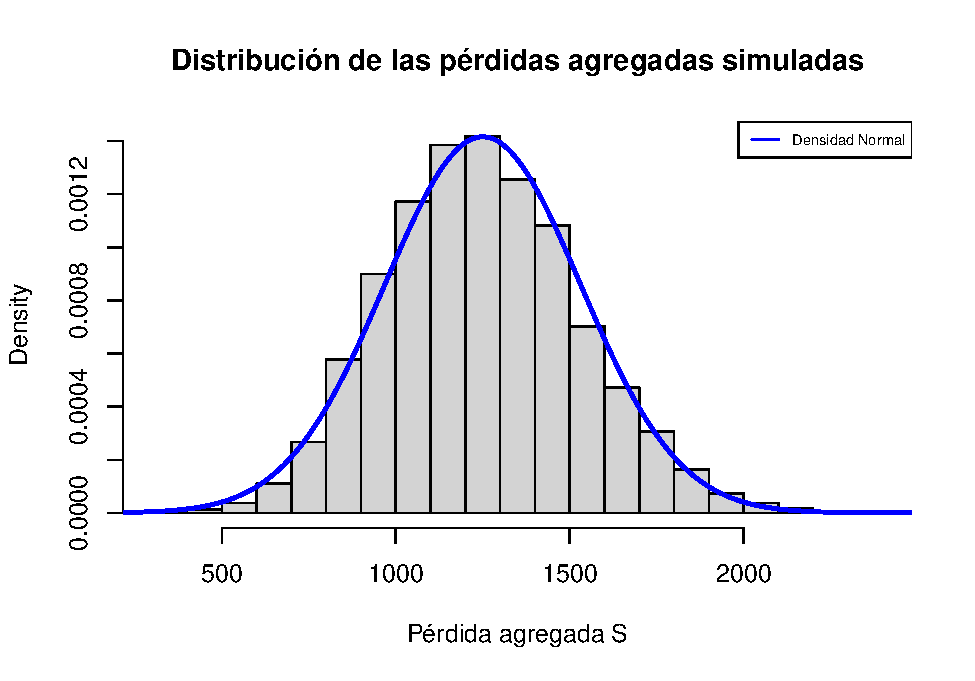
\includegraphics[width=0.7\linewidth]{LossDataAnalytics_files/figure-latex/unnamed-chunk-25-1} \end{center}

Las pérdidas simuladas son ligeramente más asimétricas a la derecha que la distribución normal, con una cola a la derecha más pesada. Lo anterior explicaría el hecho que el estimador de \(\Pr(S_N > 2000)\) de la aproximación normal es menor que el estimador basado en la simulación.

\begin{center}\rule{0.5\linewidth}{0.5pt}\end{center}

\hypertarget{efectos-de-la-modificaciuxf3n-de-las-coberturas}{%
\section{Efectos de la Modificación de las Coberturas}\label{efectos-de-la-modificaciuxf3n-de-las-coberturas}}

\hypertarget{impacto-de-la-exposiciuxf3n-en-la-frecuencia}{%
\subsection{Impacto de la exposición en la frecuencia}\label{impacto-de-la-exposiciuxf3n-en-la-frecuencia}}

Esta sección se centra en un modelo de riesgo individual para el número de siniestros. Recordemos que el modelo de riesgo individual implica un número fijo de contratos \(n\) y variables aleatorias de pérdidas independientes \(X_i\). Considere el número de siniestros de un grupo de pólizas \(n\):

\[S=X_1+\cdots+X_n\]
donde se asume que las \(X_i\) son \emph{iid} que representan el número de siniestros de cada póliza \(i\). En este caso, la exposición de la cartera es \(n\), utilizando la póliza como base de exposición. La \emph{pgf} de \(S\) es
\[\begin{aligned}
P_{S}(z)&={\rm E}(z^S)={\rm E}\left(z^{\sum_{i=1}^nX_i}\right)\\
&=\prod_{i=1}^n{\rm E}(z^{X_i})=[P_X(z)]^n
\end{aligned}\]

\textbf{Caso particular: Poisson.} Si \(X_i\sim Poi(\lambda)\), su \emph{pgf} es \(P_X(z)=e^{\lambda(z-1)}\). Entonces la \emph{pgf} de \(S\) es
\[P_{S}(z)=[e^{\lambda(z-1)}]^n=e^{n\lambda(z-1)}.\]
Por tanto \(S\sim Poi(n\lambda)\). Es decir, la suma de \(n\) variables aleatorias de Poisson independientes, cada una de media \(\lambda\), sigue una distribución de Poisson de media \(n\lambda\).

\begin{center}\rule{0.5\linewidth}{0.5pt}\end{center}

\textbf{Caso particular: Binomial Negativa.} Si \(X_i\sim NB(\beta,r)\), su \emph{pgf} es \(P_X(z)=[1-\beta(z-1)]^{-r}\). Entonces la \emph{pgf} de \(S\) es
\[P_{S}(z)=[[1-\beta(z-1)]^{-r}]^n=[1-\beta(z-1)]^{-nr}.\]
Por tanto \(S\sim NB(\beta,nr)\).

\begin{center}\rule{0.5\linewidth}{0.5pt}\end{center}

\textbf{Ejemplo 5.5.1.}
Supongamos que el número de siniestros por vehículo sigue una Poisson con media \(\lambda\). Dados los siguientes datos sobre el número observado de siniestros para cada hogar, estima \(\lambda\) por máxima verosimilitud.

\[
{\small 
\begin{matrix}
\begin{array}{c|c|c}
  \hline
  \text{Hogar ID} & \text{Número de vehículos} & \text{Número de siniestros} \\
  \hline
  1 & 2 & 0 \\
  2 & 1 & 2 \\
  3 & 3 & 2 \\
  4 & 1 & 0 \\
  5 & 1 & 1 \\
  \hline
\end{array}
\end{matrix}
}
\]

Mostrar Solución de Ejemplo

\leavevmode\hypertarget{toggleExampleAggLoss.5.1}{}%
\textbf{Solución.}
Cada uno de los 5 hogares tiene un número de exposiciones \(n_j\) (número de vehículos) y un número de siniestros \(S_j\), \(j=1,...,5\). En cada hogar el número de siniestros \(S_j \sim Poi (n_j \lambda)\). La función de verosimilitud es

\[\begin{aligned}
L(\lambda) &= \prod_{j=1}^5 \Pr(S_j=s_j) = \prod_{j=1}^5 \frac{e^{-n_j\lambda} (n_j \lambda)^{s_j}}{s_j!} \\
&= \left(\frac{e^{-2\lambda} (2 \lambda)^{0}}{0!} \right)
\left(\frac{e^{-1\lambda} (1 \lambda)^{2}}{2!} \right)
\left(\frac{e^{-3\lambda} (3 \lambda)^{2}}{2!} \right)
\left(\frac{e^{-1\lambda} (1 \lambda)^{0}}{0!} \right)
\left(\frac{e^{-1\lambda} (1 \lambda)^{1}}{1!} \right) \\
&\propto e^{-8\lambda} \lambda^5
\end{aligned}\]

Tomando el logaritmo de verosimilid, se tiene

\[\begin{aligned}
l(\lambda) = \log L(\lambda) = -8\lambda + 5\log(\lambda)
\end{aligned}\]
Igualando a cero la primera derivada del logaritmo de verosimilitud, se obtiene
\(\hat{\lambda} = \frac{5}{8}\)

\begin{center}\rule{0.5\linewidth}{0.5pt}\end{center}

Si la exposición de la cartera cambia de \(n_1\) a \(n_2\), se puede establecer la siguiente relación entre el número total de siniestros: \[P_{S_{n_2}}(z)=[P_X(z)]^{n_2}=[P_X(z)^{n_1}]^{n_2/n_1}=P_{S_{n_1}}(z)^{n_2/n_1}.\]

\hypertarget{S:MS:DedImpactClmFreq}{%
\subsection{Impacto de los deducibles en la frecuencia de siniestros}\label{S:MS:DedImpactClmFreq}}

Esta sección examina el efecto de los deducibles en la frecuencia de los siniestros. Intuitivamente, si se introduce un deducible en la póliza, disminuirán los siniestros reclamados ya que no se reclamará si la cuantía reclamada es inferior al deducible. Incluso si el asegurado realiza la reclamación, puede que no se realice ningún pago en la póliza, ya que puede denegarse el siniestro o que la cuantía del mismo se determine finalmente por debajo del deducible. Denotemos \(N^L\) el número de pérdidas (es decir, el número de siniestros sin deducible), y \(N^P\) el número de pagos cuando se establece un deducible \(d\). El objetivo es identificar la distribución de \(N^P\) dada la distribución de \(N^L\). A continuación se demuestra que la relación entre \(N^L\) y \(N^P\) puede establecerse en el marco del modelo de riesgo agregado.

Cabe señalar que, en ocasiones, cambios en los deducibles podrían afectar al comportamiento de siniestralidad del asegurado. Suponemos aquí que esto no ocurre, es decir, que las distribuciones subyacentes de pérdidas, tanto para la frecuencia como para la severidad, se mantienen sin cambios cuando varía el deducible.

Dado que ocurren \(N^L\) pérdidas, suponemos que \(X_1,X_2\ldots,X_{N^L}\) son las cuantías asociadas de las pérdidas. Para \(j=1,\ldots,N^L\), se define
\begin{eqnarray*}
I_j&=&
\left \{
\begin{array}{cc}
1 & \text{si} ~X_j>d\\
0 & \text{el resto de casos}\\
\end{array}
\right..
\end{eqnarray*}

Por tanto, se establece
\[N^P=I_1+I_2+\cdots+I_{N_L},\]

Es decir, el número total de pagos es igual al número de pérdidas por encima del valor del deducible. Dado que las \(I_j\) son variables aleatorias de Bernoulli independientes con probabilidad de éxito \(v=\Pr(X>d)\), la suma de un \emph{número fijo} de estas variables es una variable aleatoria binomial. Condicionado a \(N^L\), \(N^P\) sigue una distribución binomial, es decir, \(N^P | N^L \sim Bin(N^L, v)\), donde \(v=\Pr(X>d)\). Lo anterior implica que
\[\begin{aligned}
\mathrm{E}\left(z^{N^P}|N^L\right)&= \left[ 1+v(z-1)\right]^{N^L}
\end{aligned}\]

Por tanto, la \emph{pgf} de \(N^P\) es
\[\begin{aligned}
P_{N^P}(z)&= \mathrm{E}_{N^P}\left(z^{N^P}\right)=\mathrm{E}_{N^L}\left[\mathrm{E}_{N^P}\left(z^{N^P}|N^L\right)\right]\\
&= \mathrm{E}_{N^L}\left[(1+v(z-1))^{N^L}\right]\\
&= P_{N^L}\left(1+v(z-1)\right)
\end{aligned}\]

Así, se puede definir la \emph{pgf} de \(N^P\) como la \emph{pgf} de \(N^L\), evaluada en un nuevo argumento \(z^* = 1+v(z-1)\). Esto es, \(P_{N^P}(z)=P_{N^L}(z^*)\).

\textbf{Casos particulares:}

\begin{itemize}
\item
  \(N^L\sim Poi (\lambda)\). La \emph{pgf} de \(N^L\) es \(P_{N^L}=e^{\lambda(z-1)}\). De este modo, la \emph{pgf} de \(N^P\) es
  \[\begin{aligned}
  P_{N^P}(z) &= e^{ \lambda(1+v(z-1)-1)} \\
  &= e^{\lambda v(z-1)} ,
  \end{aligned}\]\\
  Por tanto, \(N^P \sim Poi(\lambda v)\). Esto significa que el número de pagos tiene la misma distribución que el número de pérdidas, pero con un número esperado de pagos igual a \(\lambda v = \lambda \Pr(X>d)\).
\item
  \(N^L \sim NB(\beta, r)\). La \emph{pgf} de \(N^L\) es \(P_{N^{L}}\left( z\right) =\left[ 1-\beta \left( z-1\right)\right]^{-r}\). De este modo, la \emph{pgf} de \(N^P\) es
  \[\begin{aligned}
  P_{N^P}(z)&= \left( 1-\beta (1+v(z-1)-1)\right)^{-r}\\
  &= \left( 1-\beta v(z-1)\right)^{-r},
  \end{aligned}\]
  Por tanto, \(N^P \sim NB(\beta v, r)\). Esto significa que el número de pagos tiene la misma distribución que el número de pérdidas, pero con parámetros \(\beta v\) y \(r\).
\end{itemize}

\begin{center}\rule{0.5\linewidth}{0.5pt}\end{center}

\textbf{Ejemplo 5.5.2.}
Supongamos que las pérdidas \(X_i\sim Pareto(\alpha=4,\ \theta=150)\). Sabemos que la frecuencia de pérdidas es \(N^L\sim Poi(\lambda)\) y la frecuencia de pagos es \(N^{P}_1\sim Poi(0,4)\) con un deducible de valor igual a \(d_1=30\). Encontrar la distribución de la frecuencia de pagos \(N^{P}_2\) cuando el valor del deducible es \(d_2=100\).

Mostrar Solución de Ejemplo

\leavevmode\hypertarget{toggleExampleAggLoss.5.2}{}%
\textbf{Solución.}
Al ser la frecuencia de pérdidas \(N^L\) Poisson, las medias de la distribución de pérdidas \(N^L\) y la primera distribución de pagos \(N^{P}_1\) (con deducible \(d_1=30\)) se relacionan como \(0,4 = \lambda v_1\), donde
\[\begin{aligned}
&v_1 = \Pr(X > 30) = \left( \frac{150}{30+150}\right)^4=\left( \frac{5}{6}\right)^4 \\
\Rightarrow \ & \lambda = 0.4 \left( \frac{6}{5} \right)^4
\end{aligned}\]
Ahora, se puede definir la segunda distribución de pagos \(N^{P}_2\) (con deducible \(d_2=100\)) como Poisson con media \(\lambda_2 = \lambda v_2\), donde
\[\begin{aligned}
& v_2 = \Pr(X>100)=\left( \frac{150}{100+150}\right)^4=\left( \frac{3}{5}\right)^4 \\
\Rightarrow \ & \lambda_2 = \lambda v_2 = 0,4\left( \frac{6}{5} \right)^4 \left( \frac{3}{5} \right)^4 = 0,1075
\end{aligned}\]

\begin{center}\rule{0.5\linewidth}{0.5pt}\end{center}

\textbf{Ejemplo 5.5.3. Continuación.}
Ahora supongamos que la frecuencia de pérdidas es \(N^L \sim NB(\beta,\ r)\) y para el deducible \(d_1=30\), la frecuencia de pagos \(N^{P}_1\) es negativa binomial con media \(0,4\). Encontrar la media de la frecuencia de pagos \(N^{P}_2\) para el deducible \(d_2=100\).

Mostrar Solución de Ejemplo

\leavevmode\hypertarget{toggleExampleAggLoss.5.3}{}%
\textbf{Solución.}
Al ser la frecuencia de pérdidas \(N^L\) una binomial negativa, el parámetro \(\beta\) de la distribución \(N^L\) y el parámetro \(\beta_1\) de la primera distribución de pagos \(N^{P}_1\) se relacionan como \(\beta_1 = \beta v_1\), donde \[v_1 = \Pr(X > 30) = \left( \frac{5}{6} \right)^4\] Así, la media de \(N^{P}_1\) y la media de \(N^L\) se relacionan vía

\[\begin{aligned}
&0,4 =  r \beta_1 = r \left(\beta v_1\right) \\
\Rightarrow \ & r\beta = \frac{0,4}{v_1} = 0,4 \left(\frac{6}{5} \right)^4
\end{aligned}\]
Nótese que \(v_2 = \Pr(X > 100) = \left( \frac{3}{5}\right)^4\) como en el ejemplo original. Entonces, la segunda distribución de frecuencia de pagos con deducible \(d_2=100\) es \(N^{P}_2 \sim NB(\beta v_2, \ r)\) con media
\[\begin{aligned}
r (\beta v_2) = (r \beta) v_2 = 0,4 \left( \frac{6}{5}\right)^4 \left( \frac{3}{5} \right)^4 = 0,1075
\end{aligned}\]

\begin{center}\rule{0.5\linewidth}{0.5pt}\end{center}

A continuación, se examina el caso más general en el que \(N^L\) es una distribución cero modificada. Recordemos que una distribución cero modificada puede definirse en términos de una distribución no modificada (como se señala en la Sección \ref{S:zero-truncation-or-modification}). Es decir,
\[\begin{aligned}
p_k^M = c~p_k^0, {~\rm para~} k=1,2,3,\ldots,  {~\rm con~}c = \frac{1-p_0^M}{1-p_0^0},
\end{aligned}\]
donde \(p^0_k\) es la \emph{pmf} de una distribución no modificada. En el caso que \(p_0^M=0\), se denomina una distribución \emph{cero truncada}, o \(ZT\). Para otros valores arbitrarios de \(p_0^M\), es una distribución cero modificada, o \(ZM\). La \emph{pgf} de la distribución modificada se obtiene como
\[\begin{aligned}
P^M(z) &= 1-c+c~P^0(z),
\end{aligned}\]
expresada en términos de la \emph{pgf} de la distribución no modificada, \(P^0(z)\). Cuando \(N^L\) sigue una distribución cero modificada, la distribución de \(N^P\) se establece usando la misma relación anterior, \(P_{N^P}(z)=P_{N^L}\left(1+v(z-1)\right)\).

\textbf{Casos particulares:}

\begin{itemize}
\item
  \(N^{L}\) es una variable aleatoria ZM-Poisson con parámetros \(\lambda\) y \(p_0^{M}\). La \emph{pgf} de \(N^L\) es
  \[P_{N^{L}}(z)=1-\cfrac{1-p_0^{M}}{1-e^{-\lambda}}+\cfrac{1-p_0^{M}}{1-e^{-\lambda}}\left( e^{\lambda(z-1)} \right).\]
  Por tanto, la \emph{pgf} de \(N^P\) es
  \[P_{N^{P}}(z)=1-\cfrac{1-p_0^{M}}{1-e^{-\lambda}}+\cfrac{1-p_0^{M}}{1-e^{-\lambda}}\left( e^{\lambda v(z-1)} \right).\]
  Así el número de pagos sigue también una distribución ZM-Poisson con parámetros \(\lambda v\) y \(p_0^{M}\). La probabilidad en cero se puede evaluar mediante
  \({\rm Pr}(N^P=0) = P_{N^P}(0)\).
\item
  \(N^{L}\) es una variable aleatoria ZM-binomial negativa con parámetros \(\beta\), \(r\), y \(p_0^{M}\). La \emph{pgf} de \(N^L\) es
  \[P_{N^{L}}(z)=1-\cfrac{1-p_0^{M}}{1-(1+\beta)^{-r}}+\cfrac{1-p_0^{M}}{1-(1+\beta)^{-r}}\left[ 1-\beta \left( z-1\right)\right]^{-r}.\]
  Por tanto, la \emph{pgf} de \(N^P\) es
  \[P_{N^{P}}(z)=1-\cfrac{1-p_0^{M}}{1-(1+\beta)^{-r}}+\cfrac{1-p_0^{M}}{1-(1+\beta)^{-r}}\left[ 1-\beta v\left( z-1\right)\right]^{-r}.\]
  Así, el número de pagos sigue también una distribución ZM-binomial negativa con parámetros \(\beta v\), \(r\), y \(p_0^{M}\). Del mismo modo, la probabilidad en cero se puede evaluar mediante
  \({\rm Pr}(N^P=0) = P_{N^P}(0)\).
\end{itemize}

\begin{center}\rule{0.5\linewidth}{0.5pt}\end{center}

\textbf{Ejemplo 5.5.4.}
Las pérdidas agregadas se modelizan de la siguiente manera:\\
(i) El número de pérdidas sigue una distribución Poisson modificada en cero con \(\lambda=3\) y \(p_0^M = 0,5\).\\
(ii) La cuantía de la pérdida sigue una distribución Burr con \(\alpha=3, \theta=50, \gamma=1\).\\
(iii) Se introduce un deducible \(d=30\) para cada pérdida.\\
(iv) El número de pérdidas y su cuantía son independientes entre sí.

Calcular \(\mathrm{E}(N^P)\) y \(\mathrm{Var}(N^P)\).

Mostrar Solución de Ejemplo

\leavevmode\hypertarget{toggleExampleAggLoss.5.4}{}%
\textbf{Solución.}
Dado que \(N^L\) sigue una distribución ZM-Poisson con parámetros \(\lambda\) y \(p_0^M\), sabemos que \(N^P\) también sigue una distribución ZM-Poisson, pero con parámetros \(\lambda v\) y \(p_0^M\), donde

\[v = \Pr(X>30) = \left( \frac{1}{1+(30/50)} \right)^3 = 0,2441\]

Por tanto, \(N^P\) sigue una distribución ZM-Poisson con parámetros \(\lambda^\ast = \lambda v= 0,7324\) y \(p_0^M = 0,5\). Finalmente,
\[\begin{aligned}
\mathrm{E} (N^P) &= (1-p_0^M) \frac{\lambda^\ast}{1-e^{-\lambda^\ast}} = 0,5 \left( \frac{0,7324}{1-e^{-0,7324}} \right) \\
&= 0,7053 \\
\mathrm{Var} (N^P) &= (1-p_0^M) \left( \frac{\lambda^\ast[1-(\lambda^\ast + 1) e^{-\lambda^\ast}]}{(1-e^{-\lambda^\ast})^2} \right) + p_0^M(1-p_0^M) \left(\frac{\lambda^\ast}{1-e^{-\lambda^\ast}} \right)^2 \\
&= 0,5 \left( \frac{0,7324(1-1,7324 e^{-0,7324})}{(1-e^{-0,7324})^2} \right) + 0,5^2 \left( \frac{0,7324}{1-e^{-0,7324}} \right)^2 \\
&= 0,7244
\end{aligned}\]

\begin{center}\rule{0.5\linewidth}{0.5pt}\end{center}

\hypertarget{impacto-de-las-modificaciones-de-la-puxf3liza-en-la-siniestralidad-agregada}{%
\subsection{Impacto de las modificaciones de la póliza en la siniestralidad agregada}\label{impacto-de-las-modificaciones-de-la-puxf3liza-en-la-siniestralidad-agregada}}

En esta sección, se examina el efecto de un cambio en el deducible sobre los pagos agregados de una cartera de seguros. Se asume que la presencia de límites en la póliza (\(u\)), coaseguro (\(\alpha\)) e inflación (\(r\)) no tienen ningún efecto en la distribución subyacente de la frecuencia de pagos realizados por la aseguradora. Al igual que en la sección anterior, asumimos que cambios en los deducibles tampoco afectan las distribuciones subyacentes de pérdidas, ni la de frecuencia ni la de severidad.

Recordar la notación \(N^L\) para el número de pérdidas. Con la cuantía de la pérdida inicial \(X\) y el deducible de la póliza \(d\), se usa
\(N^P\) para el número de pagos (como se definió en la sección anterior \ref{S:MS:DedImpactClmFreq}). Asimismo, se define el importe en base a las pérdidas

\begin{eqnarray*}
    X^{L}&=\left\{
      \begin{array}{ll}
        0 ~, & \text{si } ~X<\cfrac{d}{1+r} \\
        \alpha[(1+r)X-d]~, & \text{si } ~\cfrac{d}{1+r}\leq X<\cfrac{u}{1+r} \\
        \alpha(u-d)~, &  \text{si } ~X \ge \cfrac{u}{1+r}\\
      \end{array}
\right.,
\end{eqnarray*}
y la cuantía en base a los pagos
\begin{eqnarray*}
    X^{P}&=\left\{
      \begin{array}{ll}
        {\rm indeterminado} ~, & \text{si }~ X<\cfrac{d}{1+r} \\
        \alpha[(1+r)X-d]~, & \text{si }~ \cfrac{d}{1+r}\leq X<\cfrac{u}{1+r} \\
        \alpha(u-d)~, &  \text{si } ~ X \ge \cfrac{u}{1+r}\\
      \end{array}
\right..
\end{eqnarray*}
Aquí, \(r\), \(u\), y \(\alpha\) representan la tasa de inflación, el límite de la póliza y el coseguro, respectivamente. Por lo tanto, los costes agregados (cuantías de los pagos) pueden expresarse ya sea en base a pérdidas o a pagos:

\[\begin{aligned}
S &= X^L_1 + \cdots + X^L_{N^L} \\
&=X^P_1 + \cdots + X^P_{N^P} ~.
\end{aligned}\]

Los fundamentos del modelo de riesgo colectivo pueden aplicarse. Por ejemplo, se tiene que:
\[\begin{aligned}
  {\rm E}(S) &= {\rm E}\left(N^L\right) {\rm E}\left(X^L\right) = {\rm E}\left(N^P\right) {\rm E}\left(X^P\right)\\
  {\rm Var}(S) &= {\rm E}\left(N^L\right) {\rm Var}\left(X^L\right) + \left[{\rm E}\left(X^L\right)\right]^2 {\rm Var}(N^L) \\
  &= {\rm E}\left(N^P\right) {\rm Var}\left(X^P\right) + \left[{\rm E}\left(X^P\right)\right]^2 {\rm Var}(N^P)\\
  M_S(z)&=P_{N^L}\left[M_{X^L}(z)\right]=P_{N^P}\left[M_{X^P}(z)\right]
\end{aligned}\]

\begin{center}\rule{0.5\linewidth}{0.5pt}\end{center}

\textbf{Ejemplo 5.5.5. Pregunta Examen Actuarial.}
Una póliza dental colectiva sigue una distribución binomial negativa en el número de siniestros con media 300 y varianza 800. La severidad inicial se indica en la siguiente tabla:

\[
{\small 
\begin{matrix}
  \begin{array}{ c | c }
    \hline
      \text{Severidad} & \text{Probabilidad}\\ \hline
    40 & 0.25\\
    80 & 0.25\\
    120 & 0.25\\
    200 & 0.25\\
    \hline
  \end{array}
\end{matrix}
}
\]

Se espera que la severidad aumente un 50\% sin cambiar de frecuencia. Se introduce un deducible de 100 por siniestro. Calcular el valor esperado de la pérdida agregada \(S\) después de estos cambios.

Mostrar Solución de Ejemplo

\leavevmode\hypertarget{toggleExampleAggLoss.5.5}{}%
\textbf{Solución.}
El coste por pérdida con un incremento en la severidad del 50\% y un deducible por siniestro de 100 es
\begin{eqnarray*}
X^L &=&
\left\{
\begin{array}{cc}
0 & 1,5x<100 \\
1,5x-100 & 1,5x\ge 100\\
\end{array}
\right.
\end{eqnarray*}
El valor esperado es
\[\begin{aligned}
\mathrm{E}(X^L) &= \frac{1}{4} \left[ \left(1,5(40)-100\right)_+ +
\left(1,5(80)-100\right)_+ + \left(1,5(120)-100\right)_+ +
\left(1,5(200)-100\right)_+ \right]  \\
&= \frac{1}{4}\left[ (60-100)_+ + (120-100)_+ + (180-100)_+ + (300-100)_+\right] \\
&= \frac{1}{4}\left[ 0 + 20 + 80 + 200 \right] = 75
\end{aligned}\]
Por tanto, la pérdida agregada esperada es
\[\mathrm{E}(S)=\mathrm{E}(N) ~ \mathrm{E} \left(X^L \right)= 300 (75) = 22.500
.\]

\begin{center}\rule{0.5\linewidth}{0.5pt}\end{center}

\textbf{Ejemplo 5.5.6. Continuación.}
¿Cuál es la varianza de la pérdida agregada, \(\mathrm{Var~}(S)\)?

Mostrar Solución de Ejemplo

\leavevmode\hypertarget{toggleExampleAggLoss.5.6}{}%
\textbf{Solución.} En base a las pérdidas se tiene
\[\begin{aligned}
\mathrm{Var}(S) &= \mathrm{E}(N) ~ \mathrm{Var}\left(  X^L \right) + \left[ \mathrm{E} \left(X^L\right) \right]^2 ~ \mathrm{Var} (N)
\end{aligned}\]
donde \(\mathrm{E}(N) = 300\) y \(\mathrm{Var}(N) = 800\). Se obtiene que
\[\begin{aligned}
&\mathrm{E} \left[ (X^L)^2 \right] = \frac{1}{4} \left[ 0^2 + 20^2 + 80^2 + 200^2 \right] = 11.700 \\
\Rightarrow \ & \mathrm{Var}(X^L) = \mathrm{E} \left[ (X^L)^2 \right] - \left[ \mathrm{E}(X^L) \right]^2 = 11.700 - 75^2 = 6.075
\end{aligned}\]
Por tanto, la varianza del coste total de siniestralidad es
\[\begin{aligned}
\mathrm{Var}(S) &= 300(6.075) + 75^2 (800) = 6.322.500
\end{aligned}\]

\begin{center}\rule{0.5\linewidth}{0.5pt}\end{center}

\emph{Método alternativo: en base a los pagos.} Anteriormente, se ha calculado el coste total esperado de siniestralidad multiplicando el número esperado de pérdidas por el coste esperado \emph{por pérdida}. Recuerde que también podemos multiplicar el número esperado de pagos por el coste esperado \emph{por pago}. En este caso, tenemos

\[S=X_1^P + \cdots + X_{N_P}^P \]
La probabilidad de un pago es
\[\Pr(1,5X \ge 100)=\Pr(X \ge 66,\bar{6})=\frac{3}{4} .\]

Por tanto, el número de pagos, \(N^P\) tiene una distribución binomial negativa (véase el caso particular de la binomial negativa en Sección \ref{S:MS:DedImpactClmFreq})
con media
\[\mathrm{E}(N^P) =  \mathrm{E}(N^L)~\Pr(1,5X \geq 100) = 300 \left(\frac{3}{4} \right)=225\]
El coste por pago es
\begin{eqnarray*}
X^P &=&
\left\{
\begin{array}{ll}
\text{indeterminado}~, & \text{si }~ 1,5x<100 \\
1,5x-100~, & \text{si } ~ 1,5x\ge 100\\
\end{array}
\right.
\end{eqnarray*}
Su esperanza es
\[\mathrm{E}(X^P)=\frac{\mathrm{E}(X^L)}{\Pr(1,5X > 100)}=\frac{75}{(3/4)}=100\]
Por lo tanto, al igual que antes, la pérdida esperada agregada es
\[\mathrm{E}(S)=\mathrm{E}(X^P) ~ \mathrm{E}(N^P) =
100(225)=22.500\]

\begin{center}\rule{0.5\linewidth}{0.5pt}\end{center}

\textbf{Ejemplo 5.5.7. Pregunta Examen Actuarial.}
Una compañía asegura una flota de vehículos. Las pérdidas agregadas siguen una distribución compuesta de Poisson. El número esperado de pérdidas es 20.
Las pérdidas, independientemente del tipo de vehículo, siguen una distribución exponencial con \(\theta=200\). Para reducir el coste del seguro, se introducen dos modificaciones:\\
(i) No se asegurará a un cierto tipo de vehículos. Se estima que reducirá la frecuencia de pérdidas en un 20\(\%\).\\
(ii) Se incluirá un deducible de 100 por pérdida.

Calcular la cantidad total esperada que pagará la compañía después de las modificaciones.

Mostrar Solución de Ejemplo

\leavevmode\hypertarget{toggleExampleAggLoss.5.7}{}%
\textbf{Solución.}
En base a las pérdidas, se incluye un deducible de 100. Por tanto, el valor esperado por pérdida es
\[\begin{aligned}
\mathrm{E}( X^L) &= E[(X-100)_+] = E(X) - E(X\wedge 100) \\
&= 200 - 200(1-e^{-100/200}) = 121.31
\end{aligned}\]
Dado que la frecuencia de pérdidas se ha reducido en un 20\(\%\), el número esperado de pérdidas es
\[\mathrm{E}(N^L) = 0,8(20) = 16\]
Por tanto, la cantidad total esperada que pagará después de las modificaciones es
\[\mathrm{E}(S) = \mathrm{E}(X^L)~ \mathrm{E} (N^L) = 121,31(16) = 1.941\]

\begin{center}\rule{0.5\linewidth}{0.5pt}\end{center}

\emph{Método alternativo: en base a los pagos.} La cantidad total esperada que pagará después de las modificaciones también se puede calcular en base a los pagos. Con el deducible de 100, la probabilidad que ocurra un pago es \(\Pr(X > 100) = e^{-100/200}\). Para la severidad por pago, tomando la expresión \(\mathrm{E}(X^L)\) del ejemplo original, se tiene
\[\begin{aligned}
\mathrm{E} (X^P) = \frac{\mathrm{E} (X^L)}{\Pr(X > 100)} = \frac{200 - 200(1-e^{-100/200})}{e^{-100/200}} = 200
\end{aligned}\]

Este resultado es esperable---cabe recordar que la distribución exponencial no tiene memoria, por lo que el coste esperado de los siniestros por encima de 100 sigue distribuyéndose según una exponencial de media 200.

Ahora, tomemos la fecuencia de pagos

\[\mathrm{E} (N^P) = \mathrm{E}(N^L)~\Pr(X>100) = 16 ~e^{-100/200} = 9,7\]
Combinando ambos resultados, se obtiene la misma respuesta en base a los pagos que la obtenida anteriormente en base a las pérdidas
\[\mathrm{E}(S) = \mathrm{E} (X^P)~ \mathrm{E} (N^P)= 200(9,7) = 1.941\]

\begin{center}\rule{0.5\linewidth}{0.5pt}\end{center}

\hypertarget{AL-further-reading-and-resources}{%
\section{Otros Recursos y Colaboradores}\label{AL-further-reading-and-resources}}

\hypertarget{ejercicios-2}{%
\subsubsection{Ejercicios}\label{ejercicios-2}}

Aquí se ofrece un conjunto de ejercicios que guían al lector a través de algunos de los fundamentos teóricos de \textbf{Loss Data Analytics}. Cada tutorial se basa en una o más preguntas de los exámenes actuariales profesionales, normalmente el Examen C de la Society of Acturies.

\href{https://www.ssc.wisc.edu/~jfrees/loss-data-analytics/aggregate-loss-guided-tutorials/}{Aggregate Loss Guided Tutorials}

\hypertarget{colaboradores-2}{%
\subsubsection*{Colaboradores}\label{colaboradores-2}}
\addcontentsline{toc}{subsubsection}{Colaboradores}

\begin{itemize}
\tightlist
\item
  \textbf{Peng Shi} y \textbf{Lisa Gao}, Universidad de Wisconsin-Madison, son los principales autores de la version inicial de este capítulo. Email: \href{mailto:pshi@bus.wisc.edu}{\nolinkurl{pshi@bus.wisc.edu}} para comentarios sobre los capítulos y posibles mejoras.
\item
  Revisores de los capítulos, entre otros: Vytaras Brazauska, Mark Maxwell, Jiadong Ren, Di (Cindy) Xu.
\item
  Traducción al español: Miguel Santolino (Universitat de Barcelona)
\end{itemize}

\#\#\#TS 5.A.1. Propiedades del Modelo de Riesgo Individual \{-\}

El valor esperado de la pérdida agregada en el modelo de riesgo individual,

\[\begin{aligned}
\mathrm{E}(S_n) &=\sum_{i=1}^n ~ \mathrm{E}(X_i) = \sum_{i=1}^n ~ \mathrm{E}(I_i \times B_i) = \sum_{i=1}^n ~ \mathrm{E}(I_i) ~~ \mathrm{E}(B_i) ~~~~ \text{dada la independencia entre las } I_i \text{ y las } B_i \\
&= \sum_{i=1}^n \Pr(I_i=1) ~ \mu_i ~~~~ \text{ya que el valor esperado de la variable indicadora es igual a  la probabilidad que sea } 1 \\
&= \sum_{i=1}^n ~ q_i ~ \mu_i
\end{aligned}\]

La varianza de la pérdida agregada en el modelo de riesgo individual,

\[\begin{aligned}
\mathrm{Var}(S_n) &= \sum_{i=1}^n \mathrm{Var}(X_i) ~~~~ \text{ dada la independencia entre las } X_i \\
&= \sum_{i=1}^n ~ \left( ~ \mathrm{E}\left[ \mathrm{Var}(X_i | I_i) \right] + \mathrm{Var}\left[ \mathrm{E}(X_i|I_i) \right] ~ \right) ~~~~ \text{a partir de las formulas de varianza condicionada}  \\
&= \sum_{i=1}^n \left( q_i ~ \sigma_i^2 ~ + ~ q_i ~ (1-q_i) ~ \mu_i^2 \right)
\end{aligned}\]

Para verlo, tenga en cuenta que
\[\begin{aligned}
\mathrm{E}\left[ \mathrm{Var}(X_i | I_i) \right] &= \mathrm{Var}(X_i|I_i=0) ~ \Pr(I_i=0) + \mathrm{Var}(X_i|I_i=1) ~ \Pr(I_i=1) \\
&= q_i ~ \sigma_i^2 + (1-q_i) ~ (0) = q_i ~ \sigma_i^2, 
\end{aligned}\]

y
\[\begin{aligned}
\mathrm{Var}\left[ \mathrm{E}(X_i|I_i) \right] &= q_i ~ (1-q_i) ~ \mu_i^2~,
\end{aligned}\]

en base a la varianza de la Bernoulli ya que \(\mathrm{E}(X_i|I_i) = 0\) cuando \(I_i=0\) (probabilidad \(\Pr(I_i=0) = 1-q_i\)) y \(\mathrm{E}(X_i|I_i) = \mu_i\) cuando \(I_i=1\) (probabilidad \(\Pr(I_i=1)= q_i\)).

La función generadora de probabilidad de la pérdida agregada en el modelo de riesgo individual,

\[\begin{aligned}
P_{S_n}(z) &= \prod_{i=1}^n ~ P_{X_i}(z) ~~~~ \text{dada la independencia de las } X_i \\
&= \prod_{i=1}^n ~ \mathrm{E}(z^{~X_i}) = \prod_{i=1}^n ~ \mathrm{E}(z^{~I_i \times B_i}) = \mathrm{E} \left[ \mathrm{E}(z^{~I_i \times B_i} | I_i) \right] ~~~~ \text{por la ley de esperanza iterada} \\
&= \prod_{i=1}^n \left[ ~ E\left(z^{~I_i \times B_i} | I_i=0\right) ~ \Pr(I_i=0) + E\left(z^{~I_i \times B_i} | I_i=1\right) ~ \Pr(I_i=1) ~ \right] \\
&= \prod_{i=1}^n ~ \left[ ~ (1) ~ (1-q_i) + P_{B_i}(z) ~ q_i ~ \right] = \prod_{i=1}^n \left(~ 1-q_i + q_i ~ P_{B_i}(z) ~\right)
\end{aligned}\]

Por último, la función generadora de momentos de la pérdida agregada en el modelo de riesgo individual,

\[\begin{aligned}
M_{S_n}(t) &= \prod_{i=1}^n ~ M_{X_i}(t) ~~~~ \text{dada la independencia de las } X_i \\
&= \prod_{i=1}^n ~ \mathrm{E}(e^{t~X_i}) = \prod_{i=1}^n ~ \mathrm{E}\left(e^{~t~(I_i \times B_i)} \right) = \prod_{i=1}^n ~ \mathrm{E} \left[ \mathrm{E} \left( e^{~t~(I_i \times B_i)} | I_i \right) \right] ~~~~ \text{por la ley de esperanza iterada} \\
&= \prod_{i=1}^n ~ \left[~ \mathrm{E}\left(e^{~t~(I_i \times B_i)} | I_i=0 \right) ~ \Pr(I_i=0) + \mathrm{E}\left( e^{~t~(I_i \times B_i)} | I_i=1 \right) ~ \Pr(I_i=1) ~\right] \\
&= \prod_{i=1}^n ~ \left[ ~ (1) ~ (1-q_i) + M_{B_i}(t) ~ q_i ~ \right] = \prod_{i=1}^n \left(~ 1-q_i + q_i ~ M_{B_i}(t) ~\right)
\end{aligned}\]

\begin{center}\rule{0.5\linewidth}{0.5pt}\end{center}

\#\#\#TS 5.A.2. Relación entre las funciones generadoras de probabilidad de \(X_i\) y \(X_i^T\) \{-\}

Supongamos que \(X_i\) pertenece a la clase \((a,b,0)\) con \emph{pmf} \(p_{ik} = \Pr(X_i = k)\) para \(k=0,1,\ldots\) y \(X_i^T\) es la distribución asociada truncada en cero de la clase \((a,b,1)\) con \emph{pmf} \(p_{ik}^T = p_{ik}/(1-p_{i0})\) para \(k=1,2,\ldots\). La relación entre la \emph{pgf} de \(X_i\) y la \emph{pgf} de \(X_i^T\) es la siguiente

\[\begin{aligned}
P_{X_i}(z) &= \mathrm{E~}(z^{X_i}) = \mathrm{E}\left[  \mathrm{E}\left( z^{X_i} | X_i \right) \right] ~~~~ \text{por la ley de esperanza iterada} \\ 
&= \mathrm{E}\left( z^{X_i} | X_i=0 \right)~ \Pr(X_i=0) + \mathrm{E}\left( z^{X_i} | X_i>0 \right) ~ \Pr(X_i>0) \\
&= (1)~ p_{i0} + \mathrm{E}(z^{X_i^T}) ~ (1-p_{i0}) ~~~~ \text{dado que } (X_i | X_i>0) \text{ es la variable aleatoria truncada en cero } X_i^T \\
&= p_{i0} +(1-p_{i0}) P_{X_i^{T}}(z)
\end{aligned}\]

\begin{center}\rule{0.5\linewidth}{0.5pt}\end{center}

\#\#\#TS 5.A.3. Ejemplo 5.3.8 Función generadora de momentos de la pérdida agregada \(S_N\) \{-\}

En el caso que \(N\sim Geo(\beta)\) y \(X\sim Exp(\theta)\), se obtiene

\[\begin{aligned}
P_N (z) &=\frac{1}{1- \beta (z-1)}\\
M_{X}(t) &=\frac{1}{1-\theta t}
\end{aligned}\]

Por tanto, la \emph{mgf} de la pérdida agregada \(S_N\) es
\[\begin{aligned}
M_{S_N}(t) &= P_N [M_{X}(t)] = \frac{1}{1 - \beta \left( \frac{1}{1-\theta t} - 1\right)} \\
&= \frac{1}{1 - \beta \left( \frac{\theta t}{1-\theta t} \right)} + 1 - 1 
= 1+ \frac{\beta \left( \frac{\theta t}{1-\theta t} \right)}{1 - \beta \left( \frac{\theta t}{1-\theta t} \right)} \\
&= 1 + \frac{\beta \theta t}{(1-\theta t) - \beta \theta t} = 1+ \frac{\beta \theta t}{1-\theta t (1+\beta)} \cdot \frac{1+\beta}{1+\beta} \\
&= 1 + \frac{\beta}{1+\beta} \left[ \frac{\theta (1+\beta) t}{1-\theta(1+\beta)t} \right] \\
&= 1 + \frac{\beta}{1+\beta} \left[ \frac{1}{1-\theta(1+\beta)t} - 1 \right], \\
\end{aligned}\]
que coincide con la expresión (5.1). Para la expresión alternativa de la \emph{mgf} (5.2), se puede continuar a partir de aquí:

\[\begin{aligned}
M_{S_N}(t) &=  1 + \frac{\beta}{1+\beta} \left[ \frac{\theta (1+\beta) t}{1-\theta(1+\beta)t} \right] \\
&= \frac{1+\beta}{1+\beta} +  \frac{\beta}{1+\beta} \left[ \frac{\theta (1+\beta) t}{1-\theta(1+\beta)t} \right] \\
&= \frac{1}{1+\beta} + \frac{\beta}{1+\beta} + \frac{\beta}{1+\beta} \left[ \frac{\theta (1+\beta) t}{1-\theta(1+\beta)t} \right]  \\
&= \frac{1}{1+\beta} + \frac{\beta}{1+\beta}\left[1 + \frac{\theta (1+\beta) t}{1-\theta (1+\beta)t} \right] \\
&= \frac{1}{1+\beta} +\frac{\beta}{1+\beta} \left[ \frac{1}{1-\theta (1+\beta)t}\right]
\end{aligned}\]

\hypertarget{C:Simulation}{%
\chapter{Simulación y Remuestreo}\label{C:Simulation}}

\emph{Vista previa del capítulo.} La simulación es un método computacionalmente intenso usado para resolver problemas difíciles. En lugar de crear procesos físicos y experimentar con ellos para entender sus características operacionales, un estudio de simulación se basa en una representación computacional -- considera varias condiciones hipotéticas como inputs y resume los resultados. Aunque se trata de una simulación, un gran número de condiciones hipotéticas pueden ser rápidamente examinadas con un bajo coste. La sección \ref{S:SimulationFundamentals} introduce la simulación, una herramienta computacional maravillosa que es especialmente útil en entornos complejos multivariantes.

También podemos usar la simulación para realizar extracciones de una distribución empírica -- proceso que se llama remuestreo. El remuestreo permite valorar la incertidumbre de las estimaciones en modelos complejos. La sección \ref{S:Bootstrap} introduce el remuestreo en el contexto del bootstrapping para determinar la precisión de los estimadores.

Las secciones siguientes introducen otros temas del remuestreo. La Sección \ref{S:CrossValidation} sobre la validación cruzada muestra como usarla para la selección y validación de modelos. La sección \ref{S:ImportanceSampling} sobre la importancia del muestreo describe el remuestreo en áreas específicas de interés, como en aplicaciones actuariales con colas largas. La sección \ref{S:MCMC} sobre el método de Monte Carlo basado en cadenas de Markov (MCMC, en sus siglas en inglés) introduce la simulación y el motor del remuestreo que apunta en buena medida el análisis Bayesiano moderno.

\hypertarget{S:SimulationFundamentals}{%
\section{Fundamentos de la Simulación}\label{S:SimulationFundamentals}}

\begin{center}\rule{0.5\linewidth}{0.5pt}\end{center}

En esta sección, se muestra como:

\begin{itemize}
\tightlist
\item
  Generar realizaciones aproximadamente independientes distribuidas uniformemente
\item
  Transformar las realizaciones distribuidas uniformemente en observaciones de la distribución de probabilidad de interés
\item
  Calcular cantidades de interés y determinar la precisión de las cantidades calculadas
\end{itemize}

\begin{center}\rule{0.5\linewidth}{0.5pt}\end{center}

\hypertarget{generaciuxf3n-de-observaciones-uniformes-independientes}{%
\subsection{Generación de observaciones uniformes independientes}\label{generaciuxf3n-de-observaciones-uniformes-independientes}}

Las simulaciones que consideramos son generadas por ordenadores. La principal ventaja de este enfoque es que pueden ser replicadas, permitiéndonos realizar comprobaciones y mejorar nuestro trabajo. Naturalmente, esto también significa que no son realmente aleatorias. Sin embargo, se han desarrollado algoritmos para que los resultados se comporten como aleatorios a efectos prácticos. En concreto, pasan test de independencia sofisticados y pueden ser diseñados de modo que provengan de una única distribución -- nuestro supuesto iid, idénticamente e independientemente distribuidas, según sus siglas en inglés.

Para tener una idea de lo que estos algoritmos hacen, consideramos un método de importancia histórica.

\textbf{Generador Lineal Congruencial.} Para generar una secuencia de números aleatorios, comenzamos con \(B_0\), un valor inicial que es conocido como \emph{semilla}. Este valor se actualiza utilizando la relación recursiva
\[B_{n+1} = a B_n + c  \text{ modulo }m, ~~ n=0, 1, 2, \ldots .\]
Este algoritmo se denomina generador lineal congruencial . El caso \(c=0\) se denomina generador congruencial \emph{multiplicativo}; es particularmente útil para cálculos realmente rápidos.

Como valores ilustrativos de \(a\) y \(m\), Microsoft's Visual Basic usa
\(m=2^{24}\), \(a=1,140,671,485\), y \(c = 12,820,163\) (ver
\url{https://en.wikipedia.org/wiki/Linear_congruential_generator}). Este es el generador subyacente en la generación de números aleatorios en el programa Microsoft Excel.

La secuencia usada por el analista se define como \(U_n=B_n/m.\) El analista puede interpretar la secuencia
\{\(U_{i}\)\} como (aproximadamente) idénticamente e independientemente uniformemente distribuida en el intervalo (0,1). Para ilustrar el algoritmo, se considera lo siguiente.

\textbf{Ejemplo 6.1.1. Secuencia ilustrativa.}

Se asume \(m=15\), \(a=3\), \(c=2\) y \(B_0=1\). Entonces se tiene:

\begin{longtable}[]{@{}clc@{}}
\toprule
paso \(n\) & \(B_n\) & \(U_n\) \\
\midrule
\endhead
0 & \(B_0=1\) & \\
1 & \(B_1 =\mod(3 \times 1 +2) = 5\) & \(U_1 = \frac{5}{15}\) \\
2 & \(B_2 =\mod(3 \times 5 +2) = 2\) & \(U_2 = \frac{2}{15}\) \\
3 & \(B_3 =\mod(3 \times 2 +2) = 8\) & \(U_3 = \frac{8}{15}\) \\
4 & \(B_4 =\mod(3 \times 8 +2) = 11\) & \(U_4 = \frac{11}{15}\) \\
\bottomrule
\end{longtable}

A veces, a los resultados aleatorios generados por ordenadores se les conoce como números pseudo-aleatorios, para reflejar el hecho de que son generados por una máquina y pueden ser replicados. Es decir, a pesar de que \{\(U_{i}\)\} parece ser
i.i.d, puede ser reproducido usando el mismo valor de semilla (y el mismo algoritmo).

\textbf{Ejemplo 6.1.2. Generación de números aleatorios uniformes en \texttt{R}.}

El siguiente código muestra como generar tres números uniformes (0,1) en \texttt{R} usando el comando \texttt{runif}. La función \texttt{set.seed()} establece el valor inicial de la semilla. En muchos paquetes informáticos, la semilla inicial se establece usando el reloj del sistema, si no se especifica otra cosa.

\hypertarget{tres-variables-aleatorias-uniformes}{%
\paragraph*{Tres variables aleatorias uniformes}\label{tres-variables-aleatorias-uniformes}}
\addcontentsline{toc}{paragraph}{Tres variables aleatorias uniformes}

\begin{tabular}{c}
\hline
Uniforme\\
\hline
0.92424\\
\hline
0.53718\\
\hline
0.46920\\
\hline
\end{tabular}

\begin{center}\rule{0.5\linewidth}{0.5pt}\end{center}

El generador lineal congruencial es simplemente un método para generar valores pseudo-aleatorios. Es fácil entender y es (todavía) ampliamente usado. El generador lineal congruencial tiene limitaciones, incluyendo el hecho de que es posible detectar patrones a largo plazo en el tiempo en las secuencias que genera (es necesario recordar que se puede interpretar \emph{independencia} como una falta total de patrón funcional). No sorprende que se hayan desarrollado técnicas avanzadas para hacer frente a algunos de estos inconvenientes.

\hypertarget{S:InverseTransform}{%
\subsection{Método de la transformada inversa}\label{S:InverseTransform}}

Se parte de una secuencia de números aleatorios uniformes, y a continuación se transforma en la distribución de interés, sea \(F\). Una técnica destacada es el método de la transformada inversa, definido como

\[
X_i=F^{-1}\left( U_i \right) .
\]
Aquí, se recuerda que en la Sección 4.1.1 se ha introducido la función de distribución inversa, \(F^{-1}\), también referenciada como función cuantil. En concreto, se define como

\[
F^{-1}(y) = \inf_x ~ \{ F(x) \ge y \} .
\]
Se recuerda que \(\inf\) representa \emph{ínfimo} o el máxima cota inferior. Es en esencia el valor más pequeño de \emph{x} que satisface la desigualdad \(\{F(x) \ge y\}\). El resultado es que la secuencia \{\(X_{i}\)\} es aproximadamente \emph{iid} con función de distribución \(F\).

El resultado de la transformada inversa puede obtenerse cuando la variable aleatoria es continua, discreta o una combinación híbrida de ambas. Ahora se presenta una serie de ejemplos para ilustrar el alcance de sus aplicaciones.

\textbf{Ejemplo 6.1.3. Generar valores aleatorios exponenciales.}

Se desea generar observaciones según una distribución exponencial con parámetro de escala \(\theta\) de manera que \(F(x) = 1 - e^{-x/\theta}\). Para calcular la transformada inversa, se siguen los siguientes pasos:

\[
\begin{aligned}
 y = F(x) &\iff  y = 1-e^{-x/\theta} \\
  &\iff-\theta \ln(1-y) = x = F^{-1}(y) .
\end{aligned}
\]
Por tanto, si \(U\) tiene una distribución uniforme (0,1), entonces \(X = -\theta \ln(1-U)\) tiene una distribución exponencial con parámetro \(\theta\).

El siguiente código de \texttt{R} muestra como se puede comenzar con los mismos tres números aleatorios uniformes del \emph{Ejemplo 6.1.2} y transformarlos en variables aleatorias exponenciales independientes con media 10. Alternativamente, se puede usar directamente la función \texttt{rexp} de \texttt{R} para generar valores aleatorios según una distribución exponencial. El algoritmo que se construye en esta rutina es diferente por eso incluso con el mismo valor inicial de semilla, las realizaciones individuales pueden ser diferentes.

\hypertarget{tres-variables-aleatorias-uniformes-1}{%
\paragraph*{Tres variables aleatorias uniformes}\label{tres-variables-aleatorias-uniformes-1}}
\addcontentsline{toc}{paragraph}{Tres variables aleatorias uniformes}

\begin{tabular}{r|r|r}
\hline
Uniforme & Exponencial 1 & Exponencial 2\\
\hline
0.92424 & 25.80219 & 3.25222\\
\hline
0.53718 & 7.70409 & 8.47652\\
\hline
0.46920 & 6.33362 & 5.40176\\
\hline
\end{tabular}

\begin{center}\rule{0.5\linewidth}{0.5pt}\end{center}

\textbf{Ejemplo 6.1.4. Generar valores aleatorios Pareto.}

Se desea generar observaciones según una distribución de Pareto con parámetros \(\alpha\) y
\(\theta\) de modo que \(F(x) = 1 - \left(\frac{\theta}{x+\theta} \right)^{\alpha}\). Para calcular la transformada inversa, se pueden seguir los siguientes pasos:

\[
\begin{aligned}
 y = F(x) &\Leftrightarrow 1-y = \left(\frac{\theta}{x+\theta} \right)^{\alpha} \\
  &\Leftrightarrow \left(1-y\right)^{-1/\alpha} = \frac{x+\theta}{\theta} = \frac{x}{\theta} +1 \\
    &\Leftrightarrow \theta \left((1-y)^{-1/\alpha} - 1\right) = x = F^{-1}(y) .\end{aligned}
\]

Por tanto, \(X = \theta \left((1-U)^{-1/\alpha} - 1\right)\) tiene una distribución de Pareto con parámetros \(\alpha\) y \(\theta\).

\begin{center}\rule{0.5\linewidth}{0.5pt}\end{center}

\textbf{Justificación de la transformada inversa.} ¿Por qué la variable aleatoria \(X = F^{-1}(U)\) tiene función de distribución \(F\)?

Mostrar un fragmento de teoría

\hypertarget{ShowTheory.1}{}
\begin{center}\rule{0.5\linewidth}{0.5pt}\end{center}

Esto es fácil de establecer en el caso continuo. Dado que \(U\) es una variable aleatoria uniforme en (0,1), se sabe que \(\Pr(U \le y) = y\), para \(0 \le y \le 1\). Entonces,

\[
\begin{aligned}
\Pr(X \le x) &= \Pr(F^{-1}(U) \le x) \\
 &= \Pr(F(F^{-1}(U)) \le F(x)) \\
&= \Pr(U \le F(x)) = F(x)
\end{aligned}
\]
Tal y como es requerido. El paso clave es que \(F(F^{-1}(u)) = u\) para cada \(u\), es claramente cierto cuando \(F\) es estrictamente creciente.

\begin{center}\rule{0.5\linewidth}{0.5pt}\end{center}

Ahora se consideran algunos ejemplos discretos.

\textbf{Ejemplo 6.1.5. Generar valores aleatorios Bernoulli.}

Se desea simular variables aleatorias que siguen una distribución Bernoulli con parámetro \(p=0.85\).

\begin{figure}

{\centering 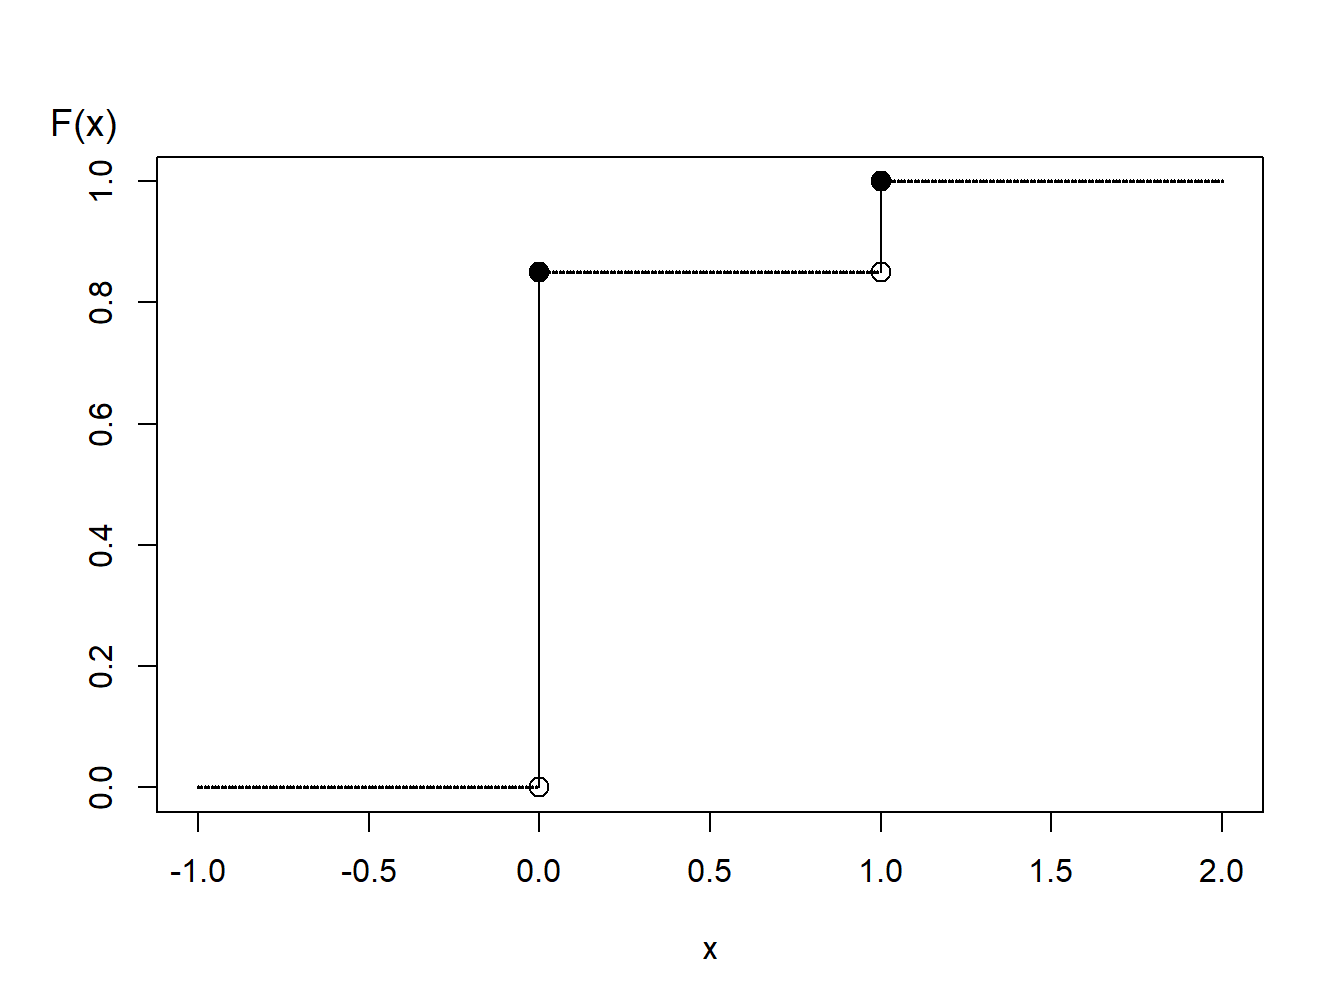
\includegraphics[width=0.5\linewidth]{LossDataAnalytics_files/figure-latex/BinaryDF-1} 

}

\caption{Función de distribución de una variable aleatoria binaria}\label{fig:BinaryDF}
\end{figure}

El gráfico de la función de distribución de la Figura \ref{fig:BinaryDF} muestra que la función cuantil puede expresarse como

\[
\begin{aligned}
F^{-1}(y) = \left\{ \begin{array}{cc}
              0 & 0<y \leq 0.85 \\
              1 & 0.85 < y  \leq  1.0 .
            \end{array} \right.
\end{aligned}
\]
Por tanto, con la transformada inversa se puede definir

\[
\begin{aligned}
X = \left\{ \begin{array}{cc}
              0 & 0<U \leq 0.85  \\
              1 &  0.85 < U  \leq  1.0
            \end{array} \right.
\end{aligned}
\]
A modo ilustrativo, se generan tres números aleatorios para obtener

\hypertarget{tres-variables-aleatorias}{%
\subsubsection*{Tres variables aleatorias}\label{tres-variables-aleatorias}}
\addcontentsline{toc}{subsubsection}{Tres variables aleatorias}

\begin{tabular}{r|r}
\hline
Uniforme & Binaria X\\
\hline
0.92424 & 1\\
\hline
0.53718 & 0\\
\hline
0.46920 & 0\\
\hline
\end{tabular}

\textbf{Ejemplo 6.1.6. Generación de valores aleatorios de una distribución discreta.}

Se considera el tiempo hasta que tiene lugar el fallo de una máquina en los primeros cinco años. La distribución de los tiempos de fallo viene dada por:

\hypertarget{distribuciuxf3n-discreta}{%
\paragraph*{Distribución discreta}\label{distribuciuxf3n-discreta}}
\addcontentsline{toc}{paragraph}{Distribución discreta}

\begin{tabular}{l|r|r|r|r|r}
\hline
  & \$\textasciitilde{}\textasciitilde{}\textasciitilde{}\textasciitilde{}\textasciitilde{}\textasciitilde{}\textasciitilde{}\textasciitilde{}\textasciitilde{}\textasciitilde{}\$ & \$\textasciitilde{}\textasciitilde{}\textasciitilde{}\textasciitilde{}\textasciitilde{}\textasciitilde{}\textasciitilde{}\textasciitilde{}\textasciitilde{}\textasciitilde{}\$ & \$\textasciitilde{}\textasciitilde{}\textasciitilde{}\textasciitilde{}\textasciitilde{}\textasciitilde{}\textasciitilde{}\textasciitilde{}\textasciitilde{}\textasciitilde{}\$ & \$\textasciitilde{}\textasciitilde{}\textasciitilde{}\textasciitilde{}\textasciitilde{}\textasciitilde{}\textasciitilde{}\textasciitilde{}\textasciitilde{}\textasciitilde{}\$ & \$\textasciitilde{}\textasciitilde{}\textasciitilde{}\textasciitilde{}\textasciitilde{}\textasciitilde{}\textasciitilde{}\textasciitilde{}\textasciitilde{}\textasciitilde{}\$\\
\hline
Tiempo & 1.0 & 2.0 & 3.0 & 4.0 & 5.0\\
\hline
Probabilidad & 0.1 & 0.2 & 0.1 & 0.4 & 0.2\\
\hline
Función de distribución \$F(x)\$ & 0.1 & 0.3 & 0.4 & 0.8 & 1.0\\
\hline
\end{tabular}

\begin{figure}

{\centering 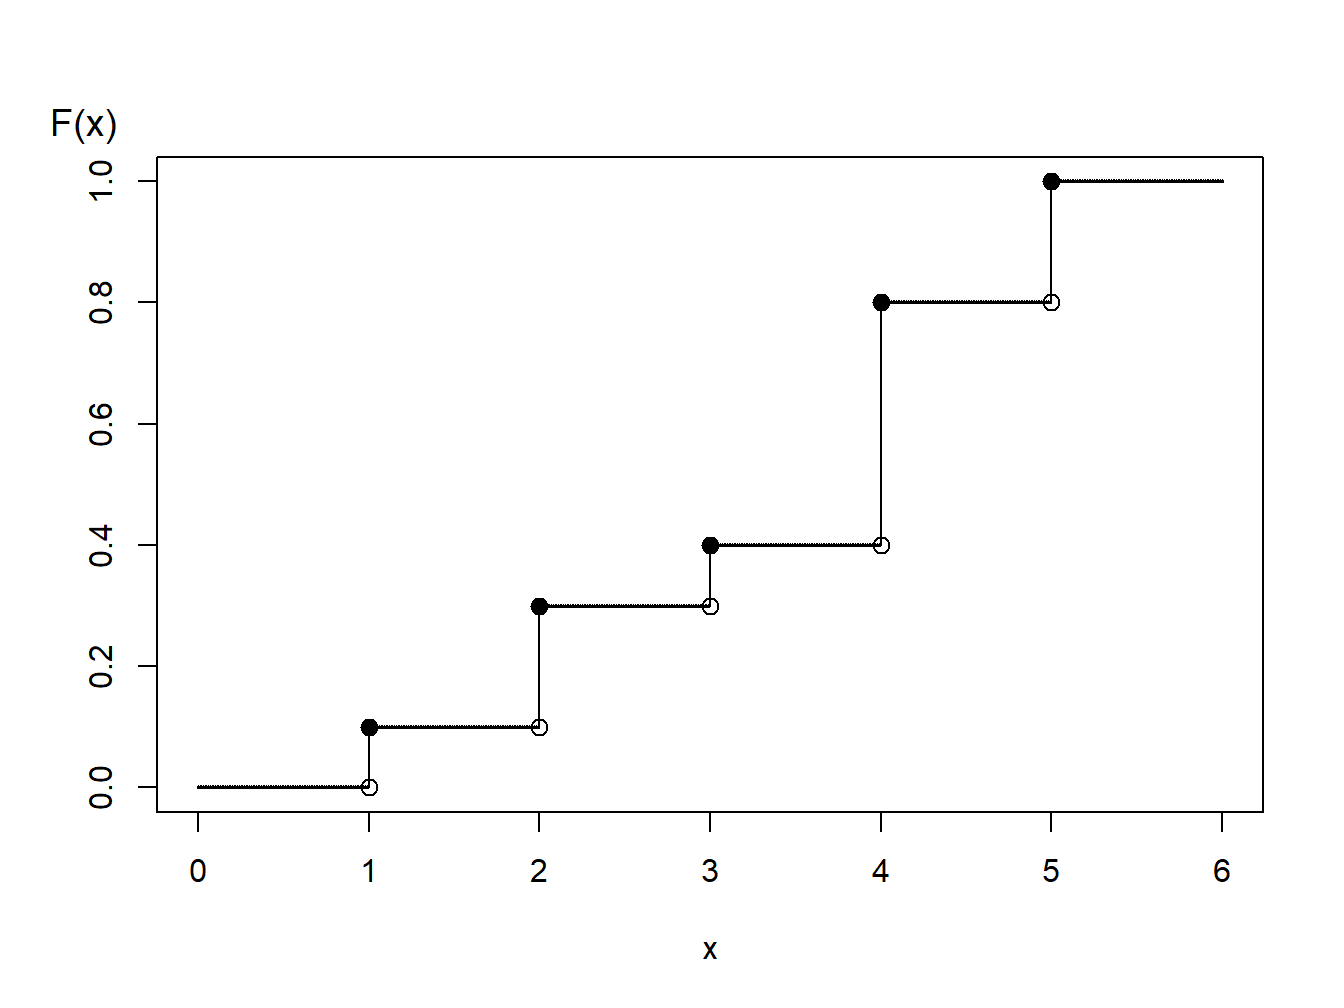
\includegraphics[width=0.6\linewidth]{LossDataAnalytics_files/figure-latex/DiscreteDF-1} 

}

\caption{Función de Distribución de una Variable Aleatoria Discreta}\label{fig:DiscreteDF}
\end{figure}

Usando el gráfico de la función de distribución en la Figura \ref{fig:DiscreteDF}, con la transformada inversa se define

\[
\small{
\begin{aligned}
X = \left\{ \begin{array}{cc}
              1 &   0<U  \leq 0.1  \\
              2 &  0.1 < U  \leq  0.3\\
              3 &  0.3 < U  \leq  0.4\\
              4 &  0.4 < U  \leq  0.8  \\
              5 &  0.8 < U  \leq  1.0     .
            \end{array} \right.
\end{aligned}
}
\]

\begin{center}\rule{0.5\linewidth}{0.5pt}\end{center}

Para variables aleatorias discretas en general puede no existir una ordenación de valores. Por ejemplo, una persona puede tener uno de los cinco posibles tipos de seguros de vida y en ese caso el siguiente algoritmo se puede usar para generar valores aleatorios:

\[
{\small
\begin{aligned}
X = \left\{ \begin{array}{cc}
  \textrm{whole life} &   0<U  \leq 0.1  \\
 \textrm{endowment} &  0.1 < U  \leq  0.3\\
\textrm{term life} &  0.3 < U  \leq  0.4\\
  \textrm{universal life} &  0.4 < U  \leq  0.8  \\
  \textrm{variable life} &  0.8 < U  \leq  1.0 .
            \end{array} \right.
\end{aligned}
}
\]

Otro analista puede usar un procedimiento alternativo como este:

\[
{\small
\begin{aligned}
X = \left\{ \begin{array}{cc}
  \textrm{whole life} &   0.9<U<1.0  \\
 \textrm{endowment} &  0.7 \leq U < 0.9\\
\textrm{term life} &  0.6 \leq U < 0.7\\
  \textrm{universal life} &  0.2 \leq U < 0.6  \\
  \textrm{variable life} &  0 \leq U < 0.2 .
            \end{array} \right.
\end{aligned}
}
\]

Ambos algoritmos producen (a largo plazo) las mismas probabilidades, e.g., \(\Pr(\textrm{whole life})=0.1\), etcétera. Por eso, ninguno es incorrecto. Es necesario tener en cuenta que hay muchos caminos para llegar a un mismo resultado. De manera similar, se podría emplear un algoritmo alternativo para valores ordenados (como los tiempos de fallo 1, 2, 3, 4, o 5, o más).

\textbf{Ejemplo 6.1.7. Generar valores aleatorios de una distribución híbrida.}

Se considera una variable aleatoria que es 0
con probabilidad 70\% y tiene distribución exponencial con parámetro
\(\theta= 10,000\) con probabilidad 30\%. En una aplicación actuarial, esto podría corresponder a un 70\% de probabilidad de no tener un siniestro y un 30\% de probabilidades de tenerlo -- si un siniestro ocurre, tiene una distribución exponencial. La función de distribución, representada en la Figura \ref{fig:MixedDF}, viene dada por

\[
\begin{aligned}
F(y) = \left\{ \begin{array}{cc}
              0 &  x<0  \\
              1 - 0.3 \exp(-x/10000) & x \ge 0 .
            \end{array} \right.
\end{aligned}
\]

\begin{figure}

{\centering 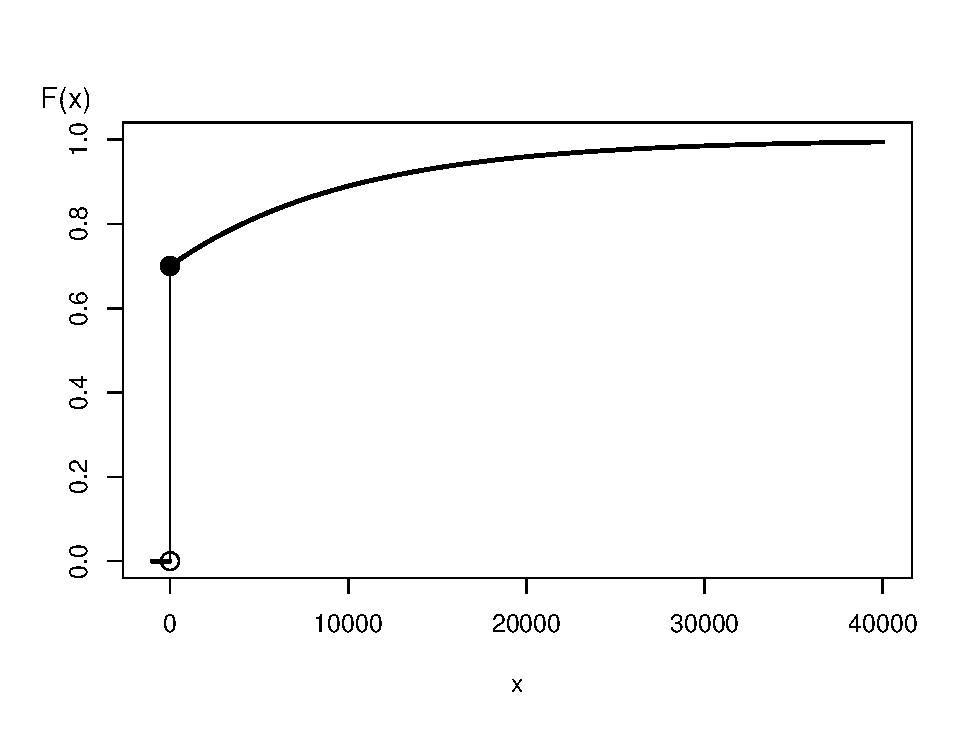
\includegraphics[width=0.6\linewidth]{LossDataAnalytics_files/figure-latex/MixedDF-1} 

}

\caption{Función de distribución de una variable aleatoria híbrida}\label{fig:MixedDF}
\end{figure}

En la Figura \ref{fig:MixedDF}, se puede ver que la transformada inversa para generar variables aleatorias con esta función de distribución es

\[
\begin{aligned}
X = F^{-1}(U) = \left\{ \begin{array}{cc}
              0 &  0< U  \leq  0.7  \\
              -1000 \ln (\frac{1-U}{0.3}) & 0.7 < U < 1 .
            \end{array} \right.
\end{aligned}
\]
Para variables aleatorias discretas e híbridas, la clave es dibujar el gráfico de la función de distribución que permita visualizar valores potenciales de la función inversa.

\hypertarget{precisiuxf3n-de-la-simulaciuxf3n}{%
\subsection{Precisión de la simulación}\label{precisiuxf3n-de-la-simulaciuxf3n}}

De las subsecciones anteriores, se sabe cómo simular valores independientes de una distribución de interés. Con estas realizaciones, se puede construir una distribución empírica y aproximar la distribución subyacente con la precisión necesaria. A medida que se introduzcan más aplicaciones actuariales en este libro, se verá que la simulación puede ser aplicada en una gran variedad de contextos.

Muchas de estas aplicaciones pueden reducirse a un problema de aproximar \(\mathrm{E~}h(X)\), donde \(h(\cdot)\) es una función conocida. En base a \(R\) simulaciones (réplicas), se obtiene \(X_1,\ldots,X_R\). A partir de esta muestra simulada, se puede calcular la media

\[
\overline{h}_R=\frac{1}{R}\sum_{i=1}^{R} h(X_i)
\]
que se usa como la aproximación simulada (estimación) de \(\mathrm{E~}h(X)\). Para estimar la precisión de esta aproximación se usa la varianza de la simulación

\[
s_{h,R}^2 = \frac{1}{R-1} \sum_{i=1}^{R}\left( h(X_i) -\overline{h}_R
\right) ^2.
\]
A partir del supuesto de independencia, el error estándar de la estimación es \(s_{h,R}/\sqrt{R}\). Esto se puede hacer tan pequeño como se desee incrementando el número de réplicas \(R\).

\textbf{Ejemplo. 6.1.8. Gestión de carteras.}

En la Sección 3.4, se explicó como calcular el valor esperado de pólizas con franquicias. Como ejemplo de algo que no puede hacerse con expresiones cerradas, se consideran ahora dos riesgos. Esta es una variación de un ejemplo más complejo que será presentado como \emph{Ejemplo 10.3.6}.

Se consideran dos riesgos patrimoniales de una empresa de telecomunicaciones:

\begin{itemize}
\tightlist
\item
  \(X_1\) - edificios, modelizado usando una distribución gamma con media 200 y parámetro de escala 100.
\item
  \(X_2\) - vehículos de motor, modelizado con una distribución gamma con media 400 y parámetro de escala 200.
\end{itemize}

El riesgo total se denota como \(X = X_1 + X_2.\) Por simplicidad, se asume que los riesgos son independientes.

Para gestionar el riesgo, se busca la protección de un seguro. Se desea gestionar internamente cuantías pequeñas asociadas a edificios y vehículos de motor, hasta \(M\). El riesgo retenido es \(Y_{retenido}=\) \(\min(X_1 + X_2,M)\). La porción del asegurador es \(Y_{asegurador} = X- Y_{retenido}\).

Para ser más concretos, se usa \(M=\) 400 así como \(R=\) 1000000 simulaciones.

\textbf{a.} Con las especificaciones, se desea determinar la cuantía esperada de siniestros y la desviación estándar asociada de (i) lo retenido, (ii) lo aceptado por el asegurador, y (iii) la cuantía total.

Aquí está el código para las cuantías de siniestros esperadas.

\begin{verbatim}
                    Retenido Asegurador  Total
Media                 365.17     235.01 600.18
Desviación estándar    69.51     280.86 316.36
\end{verbatim}

Los resultados de estos cálculos son:

\begin{verbatim}
                    Retenido Asegurador  Total
Media                 365.17     235.01 600.18
Desviación estándar    69.51     280.86 316.36
\end{verbatim}

\textbf{b.} Para siniestros asegurados, la aproximación del error estandar de la simulación es \(s_{h,R}/\sqrt{1000000} =\) 280.86 \(/\sqrt{1000000} =\) 0.281. Para este ejemplo, la simulación es rápida y un valor grande como 1000000 es una elección fácil. En cualquier caso, para problemas complejos, el tamaño de la simulación puede ser un problema.

La Figura \ref{fig:PortfolioDF} permite visualizar el desarrollo de la aproximación a medida que aumenta el número de simulaciones.

\begin{figure}

{\centering 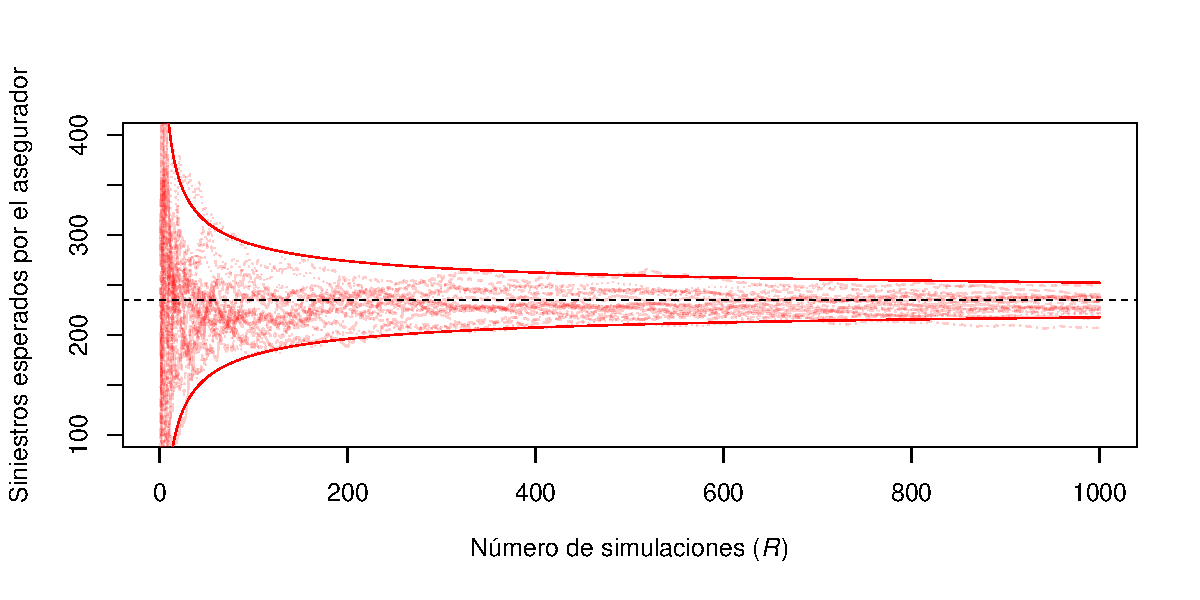
\includegraphics{LossDataAnalytics_files/figure-latex/PortfolioDF-1} 

}

\caption{Estimación del número de siniestros esperados por el asegurador versus número de simulaciones.}\label{fig:PortfolioDF}
\end{figure}

\begin{center}\rule{0.5\linewidth}{0.5pt}\end{center}

\textbf{Determinación del número de simulaciones}

¿Cuántos valores simulados se recomiendan? ¿100? ¿1,000,000? Se puede usar el teorema central del límite para responder a esta cuestión.

Como criterio para la confianza en el resultado, se supone que se desea estar dentro del 1\% de la media con 95\% de certeza. Es decir, se desea \(\Pr \left( |\overline{h}_R - \mathrm{E~}h(X)| \le 0.01 \mathrm{E~}h(X) \right) \le 0.95\). De acuerdo con el teorema central del límite, la estimación debe tener distribución aproximadamente normal, por lo que se desea que \(R\) sea suficientemente grande para satisfacer \(0.01 \mathrm{E~}h(X)/\sqrt{\mathrm{Var~}h(X)/R}) \ge 1.96\). (Se recuerda que 1.96 es el percentil 97.5 de una distribución normal estándar.) Reemplazando \(\mathrm{E~}h(X)\) y \(\mathrm{Var~}h(X)\) con sus estimaciones, se continúa la simulación hasta

\[
\frac{.01\overline{h}_R}{s_{h,R}/\sqrt{R}}\geq 1.96
\]
o equivalentemente

\begin{equation}
R \geq 38,416\frac{s_{h,R}^2}{\overline{h}_R^2}.
\label{eq:NumSimulations}
\end{equation}

Este criterio es una aplicación directa de la aproximación a la normal. Nótese que \(\overline{h}_R\) y \(s_{h,R}\) no son conocidos de antemano, por lo que se tendrán que hacer estimaciones, bien haciendo un pequeño estudio piloto de antemano o interrumpiendo el procedimiento intermitentemente para ver si el criterio se satisface.

\textbf{Ejemplo. 6.1.8. Gestión de carteras - continuación}

En este ejemplo, el número medio de siniestros es 235.011 y la correspondiente desviación estándar es 280.862. Usando la ecuación \eqref{eq:NumSimulations}, para estar dentro del 10\% de la media, se requerirán al menos 54.87 miles de simulaciones. Sin embargo, para estar dentro del 1\% se necesitarán al menos 5.49 millones de simulaciones.

\begin{center}\rule{0.5\linewidth}{0.5pt}\end{center}

\textbf{Ejemplo. 6.1.9. Elección de la aproximación.}

Una importante aplicación de la simulación es la aproximación de \(\mathrm{E~}h(X)\). En este ejemplo, se muestra que la elección de la función \(h(\cdot)\) y de la distribución de \(X\) pueden jugar un papel importante.

Se considera la siguiente pregunta: ¿cuál es \(\Pr[X>2]\) cuando \(X\) tiene una distribución de Cauchy, con densidad \(f(x) =\left(\pi(1+x^2)\right)^{-1}\), en la recta real? El valor real es

\[
\Pr\left[X>2\right] = \int_2^\infty \frac{dx}{\pi(1+x^2)} .
\]
Se puede usar una función de integración numérica en \texttt{R} (que funciona normalmente bien con integrales impropias)

que es igual a 0.14758.

Alternativamente, se pueden usar técnicas de simulación para aproximar la cantidad. Usando el cálculo, se puede comprobar que la función cuantil de una distribución de Cauchy es \(F^{-1}(y) = \tan \left( \pi(y-0.5) \right)\). Entonces, con variables uniformes (0,1) simuladas, \(U_1, \ldots, U_R\), se puede construir el estimador

\[
p_1 = \frac{1}{R}\sum_{i=1}^R \mathrm{I}(F^{-1}(U_i)>2) = \frac{1}{R}\sum_{i=1}^R \mathrm{I}(\tan \left( \pi(U_i-0.5) \right)>2) .
\]

\begin{verbatim}
[1] 0.147439
\end{verbatim}

\begin{verbatim}
[1] 0.0003545432
\end{verbatim}

Con un millón de simulaciones, se obtiene una estimación de 0.14744 con error estándar 0.355 (dividido por 1000). Se puede demostrar que la varianza de \(p_1\) es de orden \(0.127/R\).

Con otras elecciones de \(h(\cdot)\) y \(F(\cdot)\), es en realidad posible reducir la incertidumbre incluso usando el mismo número de simulaciones en \texttt{R}. Para empezar, se puede usar la simetría de la distribución de Cauchy para determinar que \(\Pr[X>2]=0.5\cdot\Pr[|X|>2]\). Con ello, se puede construir un nuevo estimador

\[
p_2 = \frac{1}{2R}\sum_{i=1}^R \mathrm{I}(|F^{-1}(U_i)|>2) .
\]

Con un millón de simulaciones, se obtiene una estimación de 0.14748 con error estándar 0.228 (dividido por 1000). Se puede demostrar que la varianza de \(p_2\) es de orden \(0.052/R\).

\textless!---Esto puede visualizarse abajo --\textgreater{}

Pero se puede ir un paso más adelante. La integral impropia puede expresarse como una integral definida por su simple propiedad de simetría (dado que la función es simétrica y la integral en la recta real es igual a \(1\))

\[
\int_2^\infty \frac{dx}{\pi(1+x^2)}=\frac{1}{2}-\int_0^2\frac{dx}{\pi(1+x^2)} .
\]
De esta expresión, una aproximación natural sería

\[
p_3 = \frac{1}{2}-\frac{1}{R}\sum_{i=1}^R h_3(2U_i), ~~~~~~\text{where}~h_3(x)=\frac{2}{\pi(1+x^2)} .
\]

Con un millón de simulaciones, se obtiene una estimación de 0.14756
con error estándar 0.169 (divido por 1000). Se puede probar que la varianza de \(p_3\) es del orden \(0.0285/R\).

Finalmente, también se puede considerar algún cambio de variable en la integral

\[
\int_2^\infty \frac{dx}{\pi(1+x^2)}=\int_0^{1/2}\frac{y^{-2}dy}{\pi(1-y^{-2})} .
\]
De esta expresión, una aproximación natural sería

\[
p_4 = \frac{1}{R}\sum_{i=1}^R h_4(U_i/2),~~~~~\text{where}~h_4(x)=\frac{1}{2\pi(1+x^2)} .
\]
La expresión parece bastante similar a la anterior,

Con un millón de simulaciones, se obtiene una estimación de 0.14759 con error estándar 0.01 (dividido por 1000). Se puede probar que la varianza de \(p_4\) es de orden \(0.00009/R\), que es mucho menor que los valores obtenidos hasta ahora!

\protect\hyperlink{tab:61}{Tabla 6.1} resume las cuatro elecciones de \(h(\cdot)\) y \(F(\cdot)\) para aproximar \(\Pr[X>2] =\) 0.14758. El error estándar varía notablemente. Por tanto, si se desea un determinado grado de precisión, entonces el \emph{número de simulaciones} depende mucho de cómo se escriban las integrales que se desean aproximar.

Tabla 6.1. Resumen de las cuatro elecciones para aproximar \(\Pr[X>2]\).

Estimador

Definición

Función de soporte

Estimación

Error estándar

\(p_1\)

\(\frac{1}{R}\sum_{i=1}^R \mathrm{I}(F^{-1}(U_i)>2)\)

\(~~~~~~F^{-1}(u)=\tan \left( \pi(u-0.5) \right)~~~~~~~\)

0.147439

0.000355

\(p_2\)

\(\frac{1}{2R}\sum_{i=1}^R \mathrm{I}(|F^{-1}(U_i)|>2)\)

\(F^{-1}(u)=\tan \left( \pi(u-0.5) \right)\)

0.147477

0.000228

\(p_3\)

\(\frac{1}{2}-\frac{1}{R}\sum_{i=1}^R h_3(2U_i)\)

\(h_3(x)=\frac{2}{\pi(1+x^2)}\)

0.147558

0.000169

\(p_4\)

\(\frac{1}{R}\sum_{i=1}^R h_4(U_i/2)\)

\(h_4(x)=\frac{1}{2\pi(1+x^2)}\)

0.147587

0.000010

\hypertarget{S:SimulationStatInference}{%
\subsection{Simulación e inferencia estadística}\label{S:SimulationStatInference}}

Las simulaciones no solo ayudan a aproximar valores esperados, sino que también son útiles para calcular otros aspectos de las funciones de distribución. En particular, son muy útiles cuando las distribuciones de los estadísticos de prueba son muy complicadas de derivar; en este caso, se pueden usar simulaciones para aproximar la distribución de referencia. Se ilustra esto con el test de Kolmogorov-Smirnov que se presenta en la Sección 4.1.2.2.

\textbf{Ejemplo. 6.1.10. Distribución del test de Kolmogorov-Smirnov.}
Se tiene disponible \(n=100\) observaciones \(\{x_1,\cdots,x_n\}\) que, sin que lo sepa el analista, han sido generadas por una distribución gamma de parámetros \(\alpha = 6\) y \(\theta=2\). El analista cree que los datos provienen de una distribución lognormal con parámetros 1 y 0.4 y desearía comprobar esta hipótesis.

El primer paso es visualizar los datos.

A partir de aquí, la Figura \ref{fig:KSTestData} proporciona un gráfico del histograma y distribución empírica. A modo de referencia, se superpone con línea rojas discontinua la distribución lognormal.

\begin{figure}

{\centering 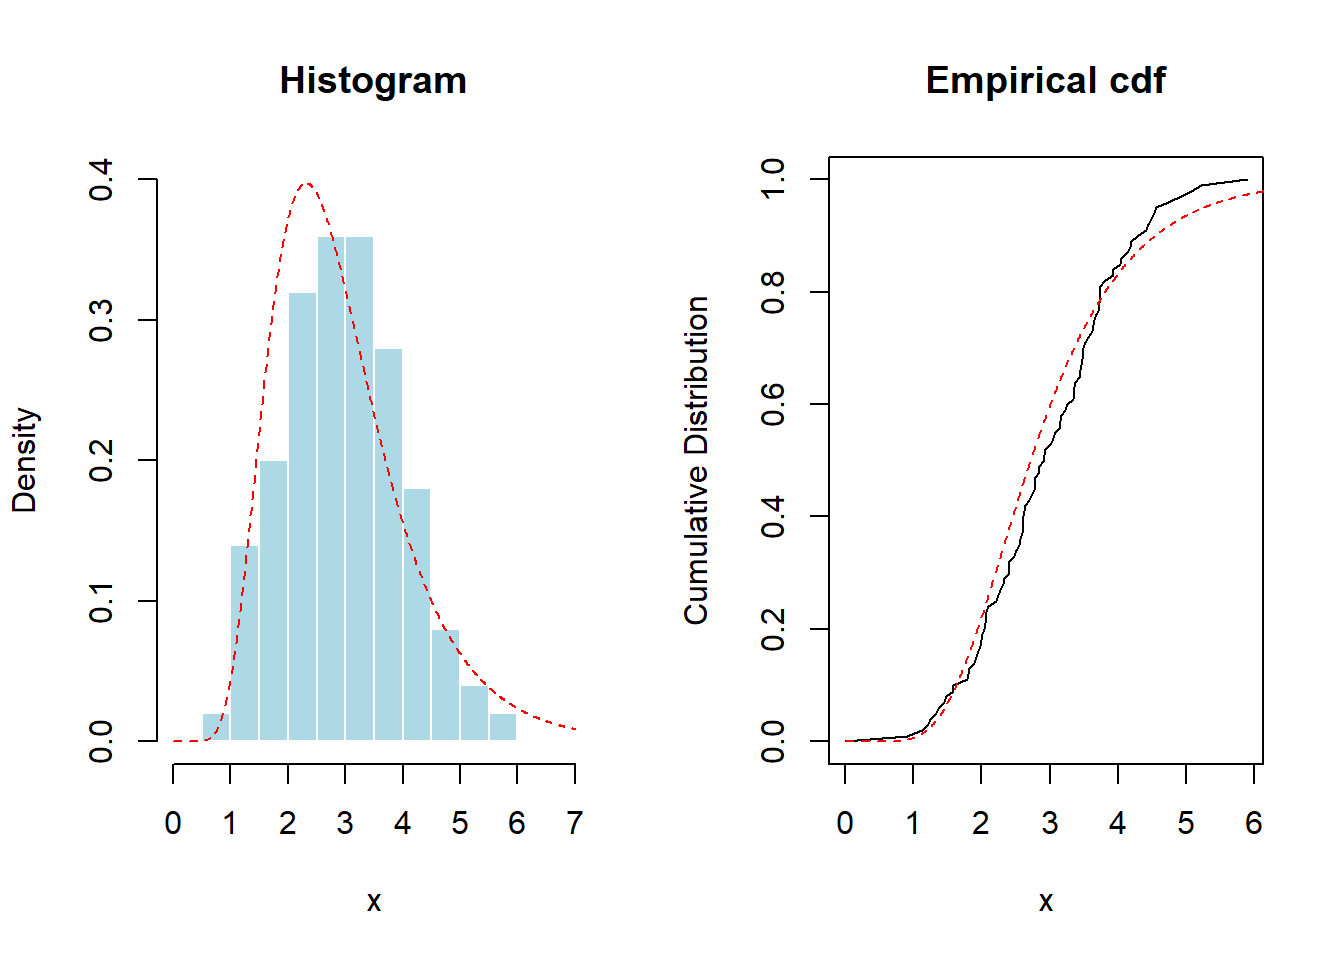
\includegraphics{LossDataAnalytics_files/figure-latex/KSTestData-1} 

}

\caption{Histograma y función de distribución empírica de los datos usados en el test de Kolmogorov-Smirnov. Las líneas rojas discontinuas son ajustadas en base a una (incorrecta) hipótesis de distribución lognormal.}\label{fig:KSTestData}
\end{figure}

Es necesario recordad qeu el estadístico de Kolmogorov-Smirnov es igual a la mayor discrepancia entre la distribución empírica y la correspondiente a la hipótesis. Esto es \(\max_x |F_n(x)-F_0(x)|\), donde \(F_0\) es la distribución lognormal de la hipótesis. Se puede calcular esto de forma directa como:

\begin{verbatim}
[1] 0.09703627
\end{verbatim}

Afortunadamente, para la distribución lognormal, \texttt{R} ha construido test que permiten determinar esto sin necesidad de realizar una programación complicada:

\begin{verbatim}
    One-sample Kolmogorov-Smirnov test

data:  x
D = 0.097037, p-value = 0.3031
alternative hypothesis: two-sided
\end{verbatim}

Sin embargo, para muchas distribuciones de interés actuarial, no se dispone de programas pre-construidos. Se puede usar la simulación para comprobar la relevancia de un estadístico de prueba. En concreto, para calcular el \(p\)-valor, se generan miles de muestras aleatorias de una distribución \(LN(1,0.4)\) (con el mismo tamaño), y se calcula empíricamente la distribución del estadístico,

\begin{Shaded}
\begin{Highlighting}[]
\NormalTok{ns }\OtherTok{\textless{}{-}} \FloatTok{1e4}
\NormalTok{d\_KS }\OtherTok{\textless{}{-}} \FunctionTok{rep}\NormalTok{(}\ConstantTok{NA}\NormalTok{,ns)}
\CommentTok{\# cálculo de los estadísticos de prueba para un valor elevado de ns (número de muestras simuladas, según sus siglas en inglés) }
\ControlFlowTok{for}\NormalTok{(s }\ControlFlowTok{in} \DecValTok{1}\SpecialCharTok{:}\NormalTok{ns) d\_KS[s] }\OtherTok{\textless{}{-}} \FunctionTok{D}\NormalTok{(}\FunctionTok{rlnorm}\NormalTok{(n,}\DecValTok{1}\NormalTok{,.}\DecValTok{4}\NormalTok{),}\ControlFlowTok{function}\NormalTok{(x) }\FunctionTok{plnorm}\NormalTok{(x,}\DecValTok{1}\NormalTok{,.}\DecValTok{4}\NormalTok{))}
\FunctionTok{mean}\NormalTok{(d\_KS}\SpecialCharTok{\textgreater{}}\FunctionTok{D}\NormalTok{(x,}\ControlFlowTok{function}\NormalTok{(x) }\FunctionTok{plnorm}\NormalTok{(x,}\DecValTok{1}\NormalTok{,.}\DecValTok{4}\NormalTok{)))}
\end{Highlighting}
\end{Shaded}

\begin{verbatim}
[1] 0.2843
\end{verbatim}

\begin{figure}

{\centering 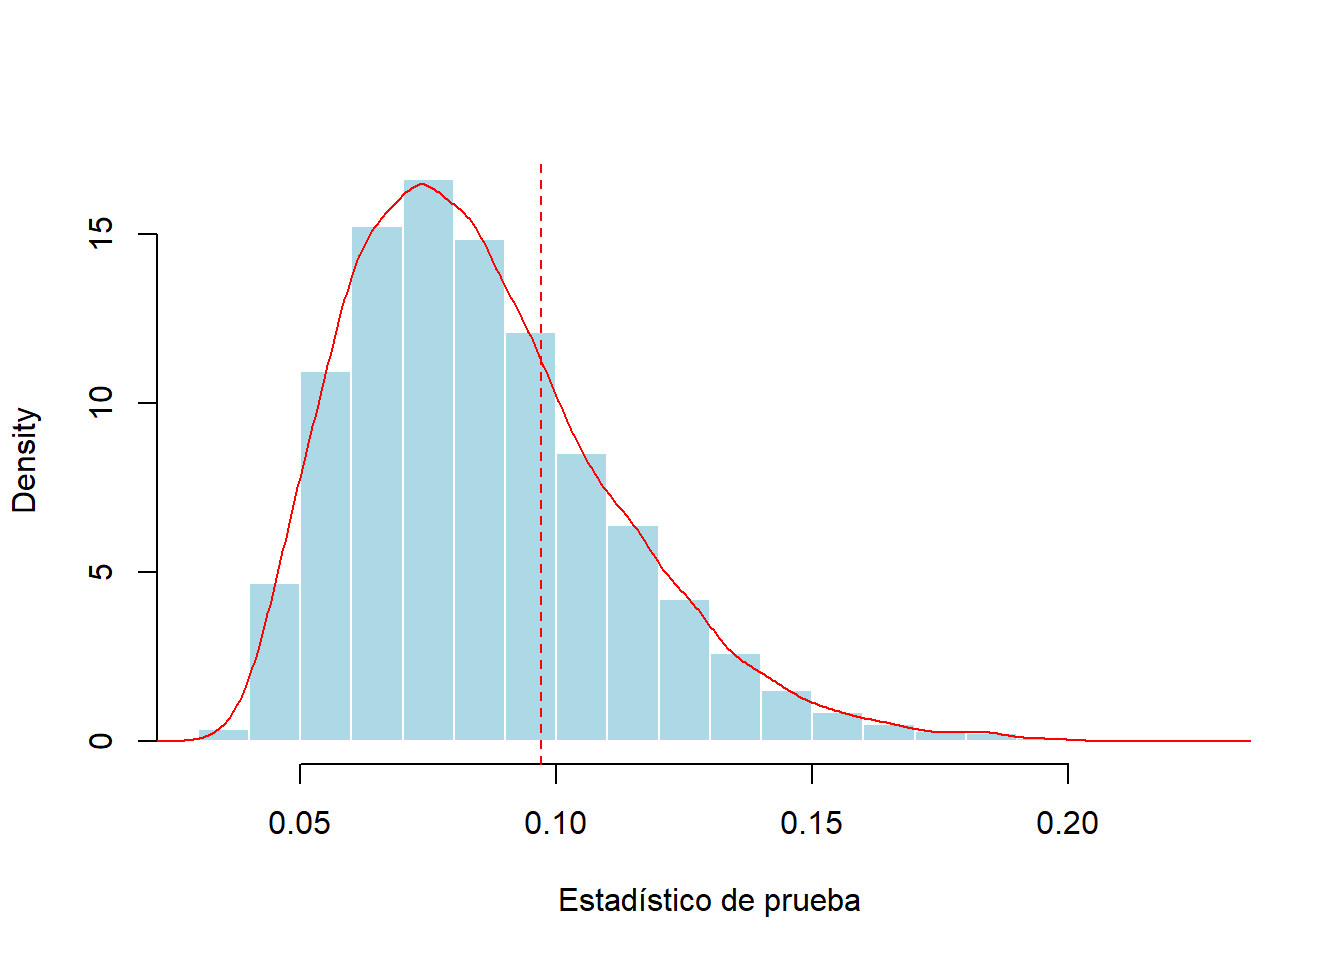
\includegraphics{LossDataAnalytics_files/figure-latex/KSSimulatedDistribution-1} 

}

\caption{Distribución simulada del estadístico de prueba de Kolmogorov-Smirnov. La línea roja discontinua vertical marca el estadístico de prueba para una muestra de 100.}\label{fig:KSSimulatedDistribution}
\end{figure}

La distribución simulada basada en 10,000 muestras aleatorias se resume en la Figura \ref{fig:KSSimulatedDistribution}. Aquí, el estadístico excede el valor empírico (0.09704) en 28.43\% de los escenarios, mientras que el \(p\)-valor \emph{teórico} es 0.3031. Tanto para la simulación como para los \(p\)-valores teóricos, las conclusiones son las mismas; los datos no proporcionan evidencia suficiente para rechazar la hipótesis de la distribución lognormal.

Aunque se trate solo de una aproximación, el enfoque basado en la simulación funciona en una gran variedad de distribuciones y estadísticos de prueba sin necesitar desarrollar los detalles de la teoría de base en cada situación. Se puede resumir el procedimiento para desarrollar distribuciones simuladas y \emph{p}-valores como sigue:

\begin{enumerate}
\def\labelenumi{\arabic{enumi}.}
\tightlist
\item
  Obtén una muestra de tamaño \emph{n}, es decir, \(X_1, \ldots, X_n\), de una función de distribución conocida \(F\). Calcula el estadístico de interés, denotado por \(\hat{\theta}(X_1, \ldots, X_n)\). Se le llama \(\hat{\theta}^r\) para la réplica \emph{r}ésima.
\item
  Se repite \(r=1, \ldots, R\) veces para obtener una muestra de estadísticos, \(\hat{\theta}^1, \ldots,\hat{\theta}^R\).
\item
  De la muestra de estadísticos en el paso 2, \(\{\hat{\theta}^1, \ldots,\hat{\theta}^R\}\), se calcula una medida de resumen de interés, como el \emph{p}-valor.
\end{enumerate}

\hypertarget{S:Bootstrap}{%
\section{Bootstrapping y Remuestreo}\label{S:Bootstrap}}

\begin{center}\rule{0.5\linewidth}{0.5pt}\end{center}

En esta sección, se muestra como:

\begin{itemize}
\tightlist
\item
  Generar una distribución no paramétrica bootstrap para un estadístico de interés
\item
  Usar la distribución bootstrap para generar estimaciones de la precisión del estadístico de interés, incluyendo sesgo, desviaciones estándar, e intervalos de confianza
\item
  Realizar análisis bootstrap para distribuciones paramétricas
\end{itemize}

\begin{center}\rule{0.5\linewidth}{0.5pt}\end{center}

\hypertarget{fundamentos-del-bootstrap}{%
\subsection{Fundamentos del Bootstrap}\label{fundamentos-del-bootstrap}}

La simulación presentada hasta ahora se basa en un muestreo a partir de una distribución \textbf{conocida}. La Sección \ref{S:SimulationFundamentals} mostró como usar técnicas de simulación para obtener muestras y calcular cantidades de estas distribuciones conocidas. Sin embargo, la ciencia estadística se dedica a proporcionar inferencias sobre distribuciones que son \emph{desconocidas}. Se recopilan estadísticos de resumen basados en esta distribución desconocida de una población. Pero, ¿cómo se puede realizar un muestreo de una distribución desconocida?

Naturalmente, no se pueden simular valores de una distribución desconocida pero sí que se pueden obtener valores de una muestra de observaciones. Si la muestra es una buena representación de una población, entonces nuestras extracciones simuladas de una muestra se aproximan bien a las extracciones simuladas de una población. El proceso de obtener una muestra de una muestra se llama \emph{remuestreo} o \emph{bootstrapping}.

El término bootstrap proviene de la frase (en inglés) ``pulling oneself up by one's bootstraps'' (Efron, 1979). En el remuestreo, la muestra original juega el papel de la población y las estimaciones obtenidas a partir de la muestra juegan el papel de los verdaderos parámetros de la población.

El algoritmo de remuestreo es el mismo que el introducido en la Sección \ref{S:SimulationStatInference} excepto que ahora usa extracciones simuladas de la muestra. Es común usar \(\{X_1, \ldots, X_n\}\) para denotar la muestra original y \(\{X_1^*, \ldots, X_n^*\}\) para los valores simulados. Las extracciones se realizan con reemplazamiento para que los valores simulados sean independientes entre ellos, la misma suposición que para la muestra original. Para cada muestra, también se realizan \emph{n} extracciones simuladas, el mismo valor que el tamaño muestral. Para distinguir este proceso de la simulación, es común usar \emph{B} (de bootstrap) para representar el número de muestras simuladas. También se puede escribir \(\{X_1^{(b)}, \ldots, X_n^{(b)}\}\), \(b=1,\ldots, B\) lo cual resulta más claro.
Hay dos métodos básicos de remuestreo, \emph{model-free} y \emph{model-based} (tomando sus nombres en inglés), que son, respectivamente, \emph{no paramétrico} y \emph{paramétrico}. En el enfoque no paramétrico, no se hace ninguna suposición sobre la distribución de la población de origen. Las extracciones simuladas provienen de la función de distribución empírica \(F_n(\cdot)\), por lo que cada extracción proviene de \(\{X_1, \ldots, X_n\}\) con probabilidad 1/\emph{n}.

Por contra, para el enfoque paramétrico, se asume que se tiene conocimiento de la familia de la distribución \emph{F}. La muestra original \(X_1, \ldots, X_n\) se usa para estimar los parámetros de esa familia, es decir, \(\hat{\theta}\). Entonces, las extracciones simuladas se toman de \(F(\hat{\theta})\). En la Sección \ref{S:ParametricBootStrap} se comenta este enfoque con más detalle.

\hypertarget{bootstrap-no-paramuxe9trico}{%
\subsubsection*{Bootstrap no paramétrico}\label{bootstrap-no-paramuxe9trico}}
\addcontentsline{toc}{subsubsection}{Bootstrap no paramétrico}

La idea del bootstrap no paramétrico es usar el método inverso en \(F_n\), la función de distribución empírica acumulada, representada en la Figura \ref{fig:InverseDFboot}.

\begin{figure}

{\centering 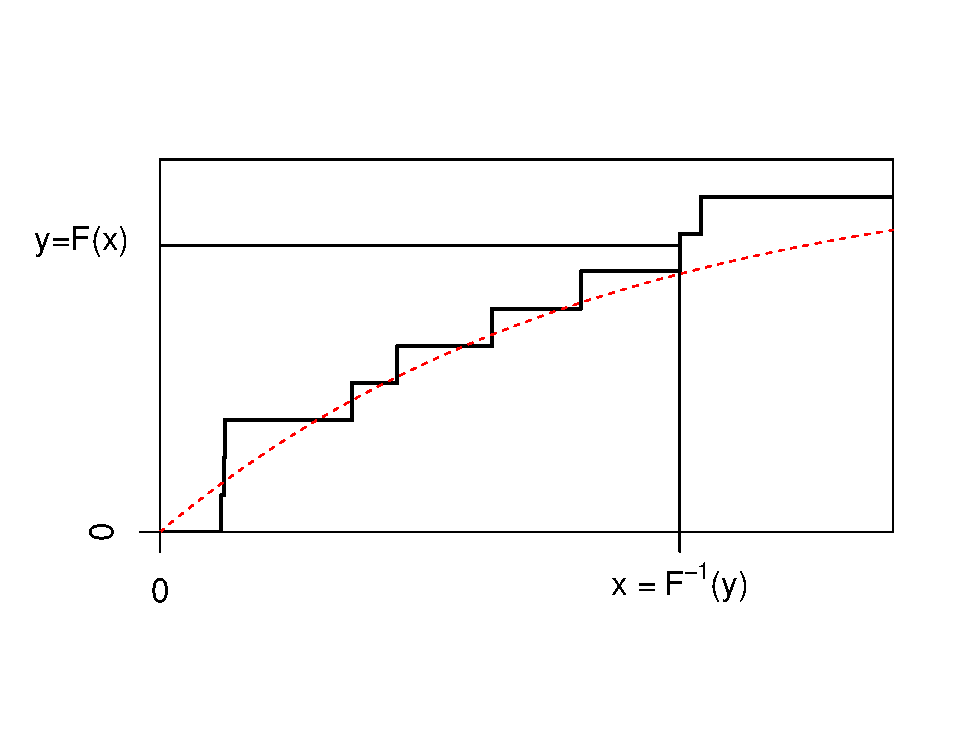
\includegraphics[width=0.6\linewidth]{LossDataAnalytics_files/figure-latex/InverseDFboot-1} 

}

\caption{Inversa de la función de distribución empírica}\label{fig:InverseDFboot}
\end{figure}

Debido a que \(F_n\) es una función escalonada, \(F_n^{-1}\) toma valores en \(\{x_1,\cdots,x_n\}\). Más concretamente, puede verse la ilustración de la Figura \ref{fig:InverseDFboot2}.
- si \(y\in(0,1/n)\) (con probabilidad \(1/n\)) se extrae el valor más pequeño (\(\min\{x_i\}\))
- si \(y\in(1/n,2/n)\) (con probabilidad \(1/n\)) se extrae el segundo valor más pequeño,
- \ldots{}
- si \(y\in((n-1)/n,1)\) (con probabilidad \(1/n\)) se extrae el mayor valor (\(\max\{x_i\}\)).

\begin{figure}

{\centering 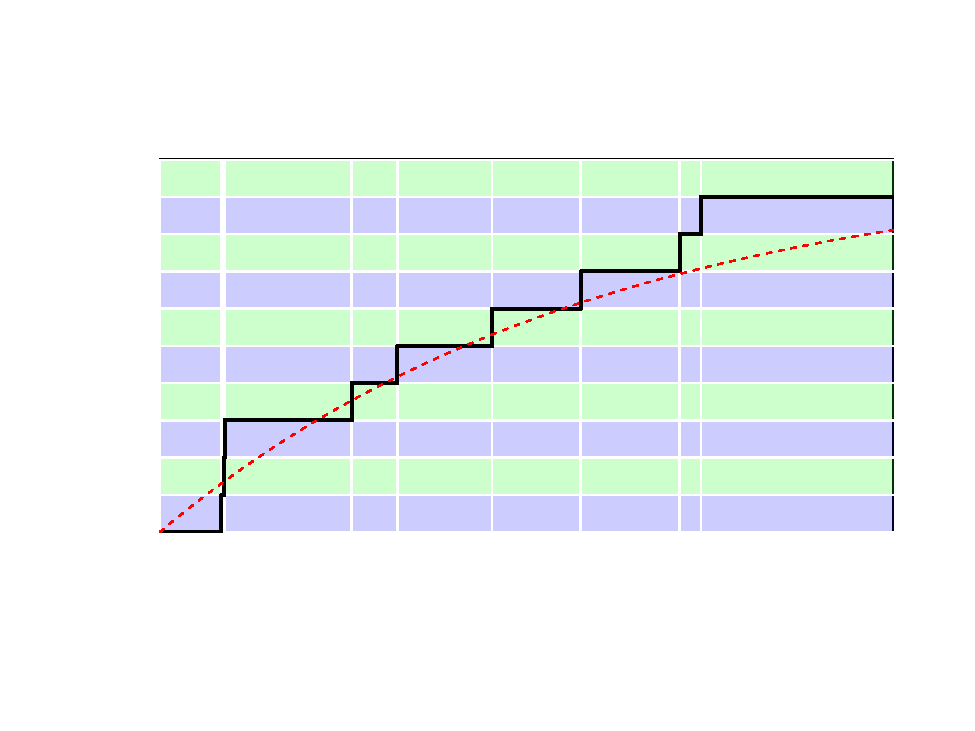
\includegraphics[width=0.6\linewidth]{LossDataAnalytics_files/figure-latex/InverseDFboot2-1} 

}

\caption{Inversa de la función de distribución empírica}\label{fig:InverseDFboot2}
\end{figure}

Usar el método inverso con \(F_n\) significa muestrear a partir de \(\{x_1,\cdots,x_n\}\), con probabilidad \(1/n\). Generar una muestra bootstrap de tamaño \(B\) significa muestrear a partir de \(\{x_1,\cdots,x_n\}\), con probabilidad \(1/n\), con reemplazamiento. A continuación, se puede consultar el siguiente código de \texttt{R} ilustrativo.

\begin{verbatim}
[1] 2.6164 5.7394 5.7394 2.6164 2.6164 7.0899 0.8823 5.7394
\end{verbatim}

Se observa que el valor 0.8388 se ha obtenido tres veces.

\hypertarget{precisiuxf3n-del-bootstrap-sesgo-desviaciuxf3n-estuxe1ndar-y-mse-error-cuadruxe1tico-medio-en-sus-siglas-en-ingluxe9s}{%
\subsection{Precisión del bootstrap: Sesgo, desviación estándar, y MSE (error cuadrático medio, en sus siglas en inglés)}\label{precisiuxf3n-del-bootstrap-sesgo-desviaciuxf3n-estuxe1ndar-y-mse-error-cuadruxe1tico-medio-en-sus-siglas-en-ingluxe9s}}

Se resume el procedimiento para el bootstrap no paramétrico como sigue:

\begin{enumerate}
\def\labelenumi{\arabic{enumi}.}
\tightlist
\item
  Para la muestra \(\{X_1, \ldots, X_n\}\), se extrae una muestra de tamaño \emph{n} (con reemplazamiento), es decir, \(X_1^*, \ldots, X_n^*\). De las extracciones simuladas se calcula el estadístico de interés, denotado como \(\hat{\theta}(X_1^*, \ldots, X_n^*)\). Se denomina \(\hat{\theta}_b^*\) para la réplica \emph{b}ésima.
\item
  Se repite esto \(b=1, \ldots, B\) veces para obtener una muestra de estadísticos, \(\hat{\theta}_1^*, \ldots,\hat{\theta}_B^*\).
\item
  Para la muestra de estadísticos en el paso 2, \(\{\hat{\theta}_1^*, \ldots, \hat{\theta}_B^*\}\), se calcula una medida de resumen de interés.
\end{enumerate}

En esta sección, se centra el interés en tres medidas de resumen, el sesgo, la desviación estándar, y el error cuadrático medio (\emph{MSE}). \protect\hyperlink{tab:62}{Tabla 6.2} resume estas tres medidas. Aquí, \(\overline{\hat{\theta^*}}\) es el promedio de \(\{\hat{\theta}_1^*, \ldots,\hat{\theta}_B^*\}\).

\[
{\small
\begin{matrix}
\text{Tabla 6.2. Medidas de resumen bootstrap}\\
\begin{array}{l|c|c|c}
\hline
\text{Medida de la población}& \text{Definición de la población}&\text{Aproximación bootstrap }&\text{Símbolo bootstrap}\\
\hline
\text{Sesgo} & \mathrm{E}(\hat{\theta})-\theta&\overline{\hat{\theta^*}}-\hat{\theta}& Bias_{boot}(\hat{\theta})  \\\hline
\text{Desviación estándar} &   \sqrt{\mathrm{Var}(\hat{\theta})}
& \sqrt{\frac{1}{B-1} \sum_{b=1}^{B}\left(\hat{\theta}_b^* -\overline{\hat{\theta^*}} \right) ^2}&s_{boot}(\hat{\theta})  \\\hline
\text{Error cuadrático medio} &\mathrm{E}(\hat{\theta}-\theta)^2 & \frac{1}{B} \sum_{b=1}^{B}\left(\hat{\theta}_b^* -\hat{\theta}
\right)^2&MSE_{boot}(\hat{\theta})\\
\hline
\end{array}\end{matrix}
}
\]

\begin{center}\rule{0.5\linewidth}{0.5pt}\end{center}

\textbf{Ejemplo 6.2.1. Siniestros con daños corporales y ratio de eliminación de pérdida.} Para mostrar cómo el bootstrap puede usarse para cuantificar la precisión de los estimadores, se retoma el Ejemplo 4.1.11 sobre los datos de siniestros con daños corporales donde se introdujo el estimador no paramétrico de la ratio de eliminación de pérdidas.

\protect\hyperlink{tab:63}{Tabla 6.3} resume los resultados de la estimación bootstrap. Por ejemplo, para \(d=14000\), se vió en el Ejemplo 4.1.11 que la estimación no paramétrica de \emph{LER} es 0.97678. Este valor tiene un sesgo estimado de 0.00018 con una desviación estándar de 0.00701. Para algunas aplicaciones, se puede desear aplicar el sesgo estimado a la estimación original para obtener un estimador corregido por el sesgo. En ello se centra el próximo ejemplo. Para esta ilustración, el sesgo es pequeño por lo que dicha corrección no es relevante.

\hypertarget{tabla-6.3.-estimaciones-bootstrap-para-el-ler-en-franquicias-seleccionadas}{%
\paragraph*{Tabla 6.3. Estimaciones bootstrap para el LER en franquicias seleccionadas}\label{tabla-6.3.-estimaciones-bootstrap-para-el-ler-en-franquicias-seleccionadas}}
\addcontentsline{toc}{paragraph}{Tabla 6.3. Estimaciones bootstrap para el LER en franquicias seleccionadas}

\begin{tabular}{r|r|r|r|r|r}
\hline
d & Estimación NP  & Sesgo bootstrap & Bootstrap SD & Límite inferior del CI (intervalo de confianza, en sus siglas en inglés) Normal al 95\% & Límite superior del CI Normal al 95\%\\
\hline
4000 & 0.54113 & 0.00011 & 0.01237 & 0.51678 & 0.56527\\
\hline
5000 & 0.64960 & 0.00027 & 0.01412 & 0.62166 & 0.67700\\
\hline
10500 & 0.93563 & 0.00004 & 0.01017 & 0.91567 & 0.95553\\
\hline
11500 & 0.95281 & -0.00003 & 0.00941 & 0.93439 & 0.97128\\
\hline
14000 & 0.97678 & 0.00016 & 0.00687 & 0.96316 & 0.99008\\
\hline
18500 & 0.99382 & 0.00014 & 0.00331 & 0.98719 & 1.00017\\
\hline
\end{tabular}

La desviación estándar bootstrap proporciona una medida de precisión. Para una aplicación de las desviaciones estándar, se puede usar la aproximación normal para crear un intervalo de confianza. Por ejemplo, la función de \texttt{R} \texttt{boot.ci} produce intervalos de confianza normales al 95\%. Se producen creando un intervalo de dos veces la amplitud de 1.95994 desviaciones estándar bootstrap, centrado en el estimador corregido por el sesgo (1.95994 es el cuantil 97.5 de la distribución normal estándar). Por ejemplo, el intervalo inferior del 95\% CI normal en \(d=14000\) es \((0.97678-0.00018)- 1.95994*0.00701\) \(= 0.96286\). Más adelante se comentan los intervalos de confianza bootstrap en la siguiente sección.

\begin{center}\rule{0.5\linewidth}{0.5pt}\end{center}

\textbf{Ejemplo 6.2.2. Estimar \(\exp(\mu)\).}

El bootstrap se puede usar para cuantificar el sesgo de un estimador, por ejemplo. Consideramos una muestra \(\mathbf{x}=\{x_1,\cdots,x_n\}\) que es iid con media \(\mu\).

Se supone que la cantidad de interés es \(\theta=\exp(\mu)\). Un estimador natural sería \(\widehat{\theta}_1=\exp(\overline{x})\). Este estimador tiene sesgo (debido a la desigualdad Jensen) pero es asintóticamente insesgado. Para nuestra muestra, la estimación es como se muestra a continuación.

\begin{verbatim}
[1] 19.13463
\end{verbatim}

Se puede usar el teorema central del límite para obtener una corrección usando

\[
\overline{X}\approx\mathcal{N}\left(\mu,\frac{\sigma^2}{n}\right)\text{ where }\sigma^2=\text{Var}[X_i] ,
\]
De modo que, con la función generatriz de momentos normal, se tiene

\[
\mathrm{E}~\exp[\overline{X}] \approx \exp\left(\mu+\frac{\sigma^2}{2n}\right) .
\]
Por tanto, se puede considerar

\[
\widehat{\theta}_2=\exp\left(\overline{x}-\frac{\widehat{\sigma}^2}{2n}\right) .
\]
Para nuestros datos, resulta lo siguiente.

\begin{verbatim}
[1] 18.73334
\end{verbatim}

Otra estrategia (que no vamos a desarrollar aquí) sería usar una aproximación de Taylor para obtener un estimador más preciso (como en el método delta),

\[
g(\overline{x})=g(\mu)+(\overline{x}-\mu)g'(\mu)+(\overline{x}-\mu)^2\frac{g''(\mu)}{2}+\cdots
\]
La alternativa que se explora es usar una estrategia bootstrap: dada una muestra bootstrap, \(\mathbf{x}^{\ast}_{b}\), sea \(\overline{x}^{\ast}_{b}\) dsu media, y se establece

\[
\widehat{\theta}_3=\frac{1}{B}\sum_{b=1}^B\exp(\overline{x}^{\ast}_{b}) .
\]
Para implementarlo, se proporciona el siguiente código.

Entonces, se puede \texttt{plot(results)} y \texttt{print(results)} para observar lo siguiente.

\begin{figure}

{\centering 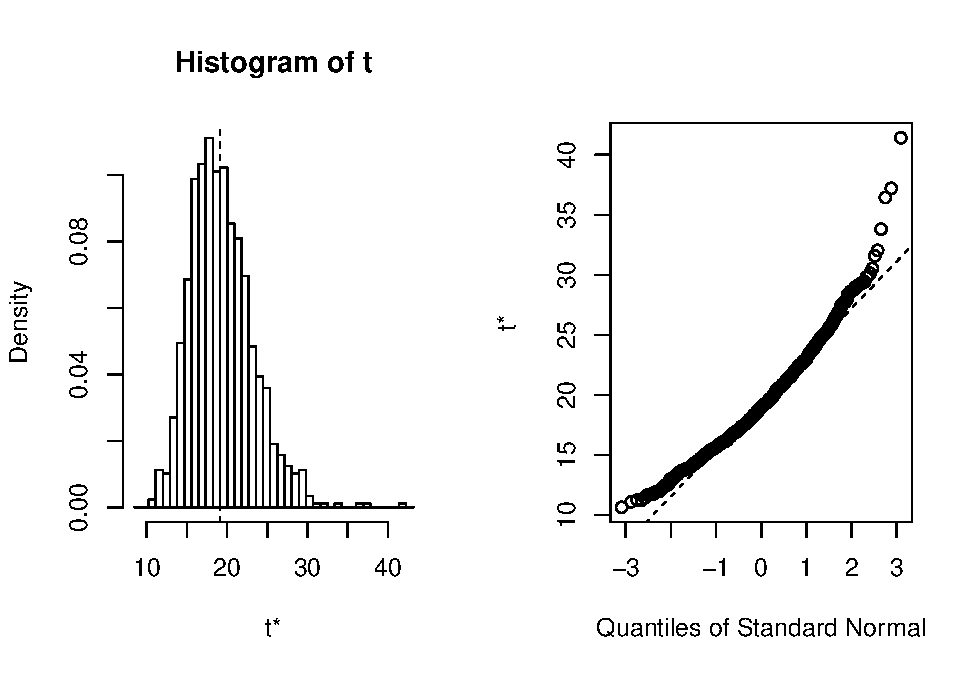
\includegraphics{LossDataAnalytics_files/figure-latex/BootstrapDistn-1} 

}

\caption{Distribución de las réplicas bootstrap. El panel de la izquierda es un histograma de réplicas. El panel de la derecha es un gráfico cuantil-cuantil, que compara la distribución bootstrap con la distribución normal estándar.}\label{fig:BootstrapDistn}
\end{figure}

\begin{verbatim}
ORDINARY NONPARAMETRIC BOOTSTRAP


Call:
boot(data = sample_x, statistic = function(y, indices) exp(mean(y[indices])), 
    R = 1000)


Bootstrap Statistics :
    original    bias    std. error
t1* 19.13463 0.2536551    3.909725
\end{verbatim}

Esto resulta en tres estimadores, el estimador bruto \(\widehat{\theta}_1=\) 19.135, la corrección de segundo orden \(\widehat{\theta}_2=\) 18.733, y el estimador bootstrap \(\widehat{\theta}_3=\) 19.388.
¿Como funciona esto con diferentes tamaños de muestra? Ahora se supone que \(x_i\)'s son generadas a partir de una distribución lognormal \(LN(0,1)\), de modo que \(\mu = \exp(0 + 1/2) = 1.648721\) y \(\theta = \exp(1.648721)\) \(= 5.200326\). Se usa la simulación para extraer los tamaños muestrales pero luego se actúa como si fueran un conjunto de observaciones realizadas. Véase el siguiente código ilustrativo.

Los resultados de la comparación se resumen en la Figura \ref{fig:BootstrapCompare}. Esta figura muestra que el estimador bootstrap está más cerca del verdadero valor del parámetro para casi todos los tamaños muestrales. El sesgo de los tres estimadores decrece al aumentar el tamaño muestral.

\begin{figure}

{\centering 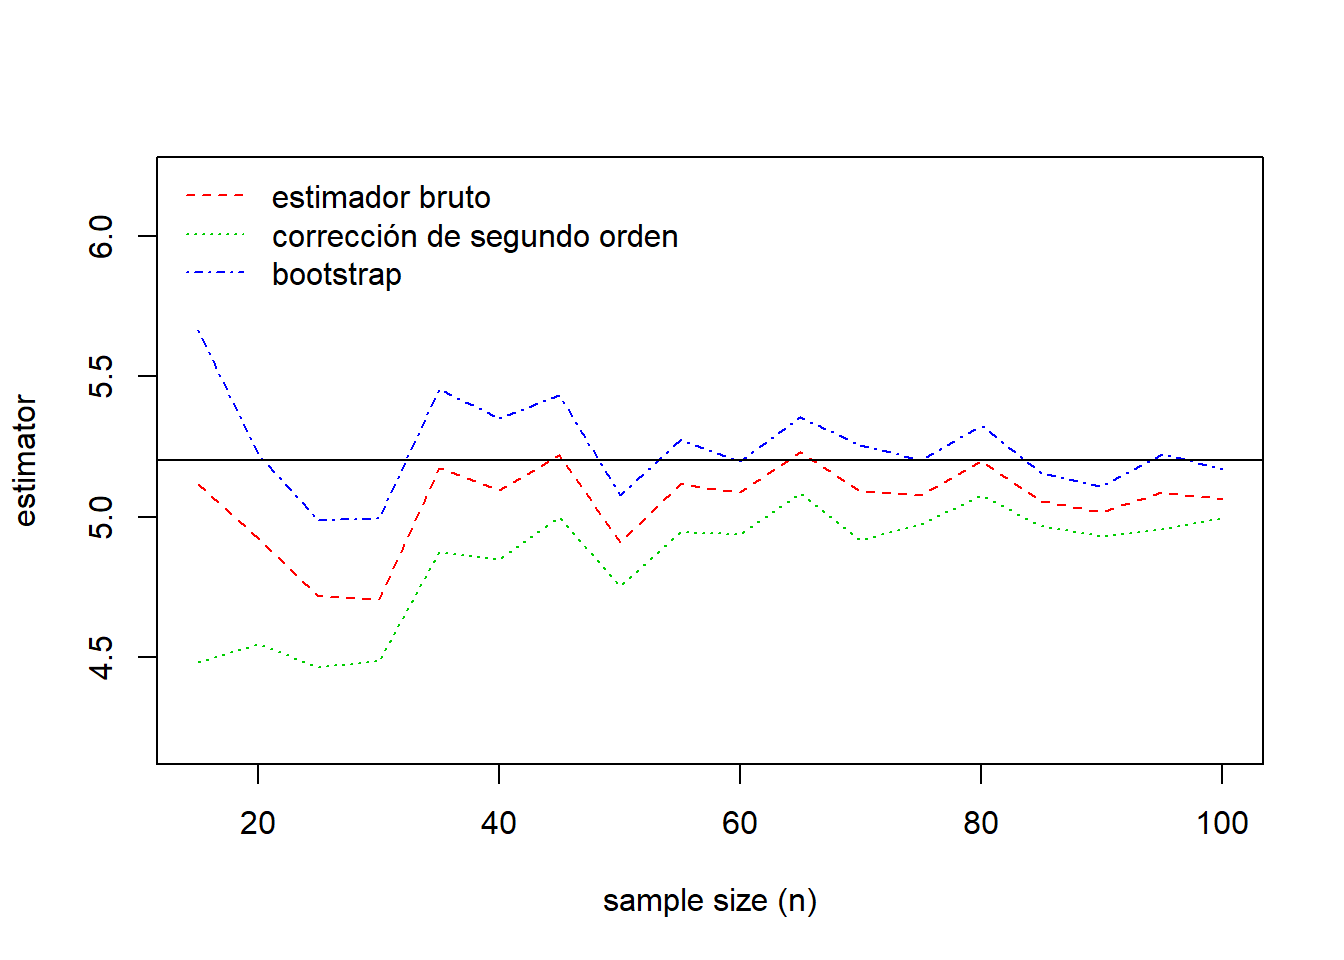
\includegraphics{LossDataAnalytics_files/figure-latex/BootstrapCompare-1} 

}

\caption{Comparación de estimaciones. El verdadero valor del parámetro viene dado por la línea continua horizontal en 5.20.}\label{fig:BootstrapCompare}
\end{figure}

\hypertarget{intervalos-de-confianza}{%
\subsection{Intervalos de confianza}\label{intervalos-de-confianza}}

El procedimiento bootstrap genera \emph{B} réplicas \(\hat{\theta}_1^*, \ldots,\hat{\theta}_B^*\) del estimador \(\hat{\theta}\). En el \emph{Ejemplo 6.2.1,} se mostró cómo usar las aproximaciones a la normal estándar para crear intervalos de confianza de los parámetros de interés. Sin embargo, dado que el interés se centra en usar el bootstrap para evitar confiar en supuestos de aproximación a la normal, no sorprende que haya disponibilidad de intervalos de confianza alternativos.

Para un estimador \(\hat{\theta}\), el intervalo de confianza \emph{básico} bootstrap es

\begin{equation} 
  \left(2 \hat{\theta} - q_U, 2 \hat{\theta} - q_L \right) ,
  \label{eq:basicBootCI}
\end{equation}

donde \(q_L\) y \(q_U\) son los cuantiles al 2.5\% inferior y superior de la muestra bootstrap \(\hat{\theta}_1^*, \ldots,\hat{\theta}_B^*\).
Para ver de dónde viene esto, se toma como punto de partida la idea de que \((q_L, q_U)\) proporciona un intervalo al 95\% para \(\hat{\theta}_1^*, \ldots,\hat{\theta}_B^*\). Por tanto, para un \(\hat{\theta}_b^*\) aleatorio, hay un 95\% de probabilidades de que \(q_L \le \hat{\theta}_b^* \le q_U\). Revirtiendo las desigualdades y añadiendo \(\hat{\theta}\) a cada lado se obtiene un intervalo al 95\%

\[
\hat{\theta} -q_U \le \hat{\theta} - \hat{\theta}_b^* \le  \hat{\theta} -q_L .
\]
Por tanto, \(\left( \hat{\theta}-q_U, \hat{\theta} -q_L\right)\) es un intervalo al 95\% para \(\hat{\theta} - \hat{\theta}_b^*\). La idea de la aproximación bootstrap indica que ello es también un intervalo al 95\% para \(\theta - \hat{\theta}\). Añadiendo \(\hat{\theta}\) a cada lado da un intervalo al 95\% en la ecuación \eqref{eq:basicBootCI}.

Hay muchos intervalos bootstrap alternativos. El más sencillo de explicar es el intervalo basado en los percentiles bootstrap que se define como \(\left(q_L, q_U\right)\). No obstante, presenta la desventaja de tener un comportamiento potencialmente pobre en las colas, lo cual puede ser un inconveniente en algunos problemas actuariales de interés.

\textbf{Ejemplo 6.2.3. Siniestros con daños corporales y medidas de riesgo.} Para ver cómo funcionan los intervalos de confianza bootstrap, se retoma los datos sobre siniestros del automóvil con daños corporales considerados en el Ejemplo 6.2.1. En lugar de la ratio de eliminación de pérdida, se desea estimar el percentil al 95\% \(F^{-1}(0.95)\) y una medida definida como
\[
TVaR_{0.95)}[X] = \mathrm{E}[X | X > F^{-1}(0.95)] .
\]
Esta medida se llama tail value-at-risk; es el valor esperado de \(X\) condicionado a que \(X\) exceda el percentil al 95\%. En la Sección 10.2 se explica como los cuantiles y el tail value-at-risk son los dos ejemplos más importantes de las llamadas \emph{medidas de riesgo}. Por el momento, se considerarán simplemente como medidas que se quieren estimar. Para el percentil, se usa el estimador no paramétrico \(F^{-1}_n(0.95)\) definido en la Sección 4.1.1.3. Para el tail value-at-risk, se usa el principio plug-in para definir el estimador no paramétrico

\[
TVaR_{n,0.95}[X] = \frac{\sum_{i=1}^n X_i I(X_i > F^{-1}_n(0.95))}{\sum_{i=1}^n I(X_i > F^{-1}_n(0.95))} ~.
\]
En esta expresión, el denominador cuenta el número de observaciones que exceden el percentil al 95\% \(F^{-1}_n(0.95)\). El numerador suma las pérdidas para aquellas observaciones que exceden \(F^{-1}_n(0.95)\). \protect\hyperlink{tab:64}{Tabla 6.4} resume el estimador para para fracciones seleccionadas.

\hypertarget{tabla-6.4.-estimaciones-bootstrap-de-cuantiles-en-fracciones-seleccionadas}{%
\paragraph*{Tabla 6.4. Estimaciones bootstrap de cuantiles en fracciones seleccionadas}\label{tabla-6.4.-estimaciones-bootstrap-de-cuantiles-en-fracciones-seleccionadas}}
\addcontentsline{toc}{paragraph}{Tabla 6.4. Estimaciones bootstrap de cuantiles en fracciones seleccionadas}

\begin{tabular}{r|r|r|r|r|r|r|r|r|r}
\hline
Fracción & Estimación NP  & Sesgo bootstrap & Bootstrap SD & Límite inferior del CI Normal al 95\% & Límite superior del CI Normal al 95\% & Límite inferior del CI básico al 95\%  & Límite superior del CI básico al 95\% & Límite inferior del CI percentil al 95\% & Límite superior del CI percentil al 95\% \\
\hline
0.50 & 6500.00 & -128.02 & 200.36 & 6235.32 & 7020.72 & 6300.00 & 7000.00 & 6000.00 & 6700.00\\
\hline
0.80 & 9078.40 & 89.51 & 200.27 & 8596.38 & 9381.41 & 8533.20 & 9230.40 & 8926.40 & 9623.60\\
\hline
0.90 & 11454.00 & 55.95 & 480.66 & 10455.96 & 12340.13 & 10530.49 & 12415.00 & 10493.00 & 12377.51\\
\hline
0.95 & 13313.40 & 13.59 & 667.74 & 11991.07 & 14608.55 & 11509.70 & 14321.00 & 12305.80 & 15117.10\\
\hline
0.98 & 16758.72 & 101.46 & 1273.45 & 14161.34 & 19153.19 & 14517.44 & 19326.95 & 14190.49 & 19000.00\\
\hline
\end{tabular}

Por ejemplo, cuando la fracción es 0.50, se observa que los cuantiles al 2.5th por abajo y por arriba de las simulaciones bootstrap son \(q_L=\) 6000 y \(q_u=\) 6700, respectivamente. Ello forma el intervalo de confianza percentil bootstrap. Con el estimador no paramétrico 6500, se obtienen los límites inferiores y superiores de los intervalos de confianza básicos 6300
y 7000, respectivamente. La \protect\hyperlink{tab:64}{Tabla 6.4} también muestra las estimaciones bootstrap del sesgo, desviación estándar, y el intervalo de confianza normal, conceptos introducidos en la sección anterior.

La \protect\hyperlink{tab:65}{Tabla 6.5} muestra cálculos similares para el tail value-at-risk. En cada caso, se observa que la desviación estándar bootstrap aumenta a medida que la fracción aumenta. Ello es un reflejo de que cada vez hay menos observaciones disponibles para estimar los cuantiles a medida que la fracción aumenta, y por lo tanto hay una mayor imprecisión. La amplitud de los intervalos de confianza también aumenta. Resulta interesante ver que no parece haber el mismo patrón en las estimaciones del sesgo.

\hypertarget{tabla-6.5.-estimaciuxf3n-bootstrap-del-tvar-en-niveles-de-riesgo-seleccionados}{%
\paragraph*{Tabla 6.5. Estimación bootstrap del TVaR en niveles de riesgo seleccionados}\label{tabla-6.5.-estimaciuxf3n-bootstrap-del-tvar-en-niveles-de-riesgo-seleccionados}}
\addcontentsline{toc}{paragraph}{Tabla 6.5. Estimación bootstrap del TVaR en niveles de riesgo seleccionados}

\begin{tabular}{r|r|r|r|r|r|r|r|r|r}
\hline
Fracción & Estimación NP & Sesgo bootstrap & Bootstrap SD & Límite inferior del CI normal al 95\%  & Límite superior del CI normal al 95\%  & Límite inferior del CI básico al 95\% & Límite superior del CI básico al 95\% & Límite inferior del CI percentil al 95\% & Límite superior del CI Percentil al 95\% \\
\hline
0.50 & 9794.69 & -120.82 & 273.35 & 9379.74 & 10451.27 & 9355.14 & 10448.87 & 9140.51 & 10234.24\\
\hline
0.80 & 12454.18 & 30.68 & 481.88 & 11479.03 & 13367.96 & 11490.62 & 13378.52 & 11529.84 & 13417.74\\
\hline
0.90 & 14720.05 & 17.51 & 718.23 & 13294.82 & 16110.25 & 13255.45 & 16040.72 & 13399.38 & 16184.65\\
\hline
0.95 & 17072.43 & 5.99 & 1103.14 & 14904.31 & 19228.56 & 14924.50 & 19100.88 & 15043.97 & 19220.36\\
\hline
0.98 & 20140.56 & 73.43 & 1587.64 & 16955.40 & 23178.85 & 16942.36 & 22984.40 & 17296.71 & 23338.75\\
\hline
\end{tabular}

\hypertarget{S:ParametricBootStrap}{%
\subsection{Bootstrap paramétrico}\label{S:ParametricBootStrap}}

La idea del bootstrap no paramétrico es remuestrear extrayendo variables independientes a partir de la función de distribución acumulada empirica \(F_n\). Por otra parte, en el bootstrap paramétrico, se extraen variables independientes de \(F_{\widehat{\theta}}\) donde la distribución subyacente se asume que pertenece a una familia paramétrica \(\mathcal{F}=\{F_{\theta},\theta\in\Theta\}\). Normalmente, los parámetros de la distribución se estiman en base a una muestra y se denotan como \(\hat{\theta}\).

\textbf{Ejemplo 6.2.4. Distribución Lognormal.} Se considera nuevamente la base de datos

El bootstrap clásico (no paramétrico) se basaba en muestras

Mientras que para el bootstrap paramétrico, se asume que la distribución de \(x_i\)'s es de una familia específica, por ejemplo la distribución lognormal.

\begin{verbatim}
    meanlog       sdlog   
  1.03630697   0.30593440 
 (0.06840901) (0.04837027)
\end{verbatim}

Entonces se realiza la extracción partiendo de esta distribución.

La Figura \ref{fig:CoefVarCompare} compara las distribuciones bootstrap para el coeficiente de variación, una de ellas basada en el enfoque no paramétrico y la otra basada en el enfoque paramétrico, asumiendo una distribución lognormal.

\begin{figure}

{\centering 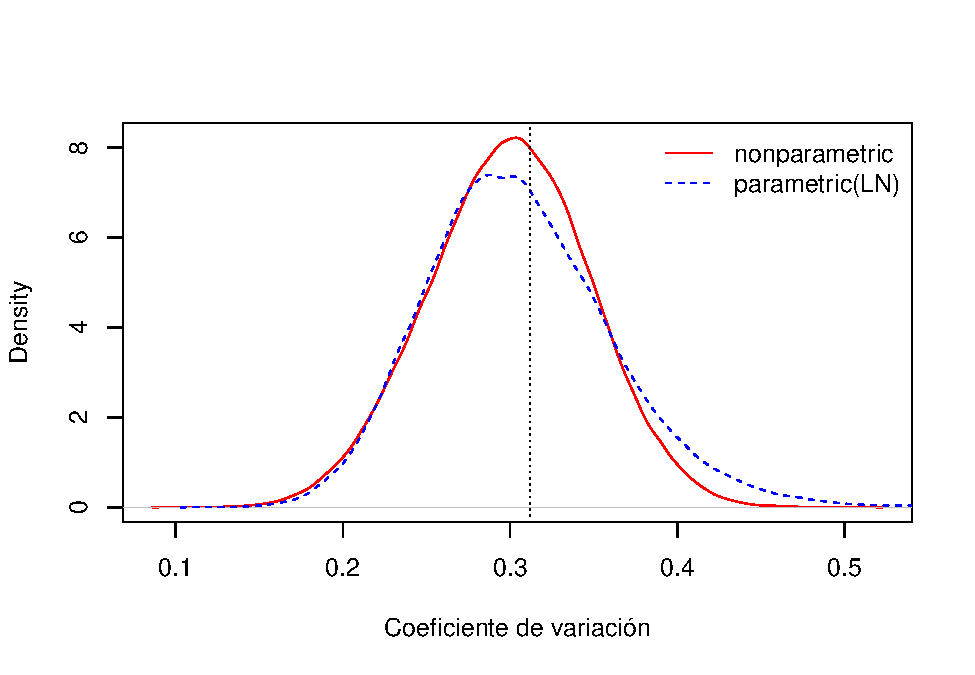
\includegraphics{LossDataAnalytics_files/figure-latex/CoefVarCompare-1} 

}

\caption{Comparación de las distribuciones Bootstrap no paramétrico y paramétrico para el coeficiente de variación}\label{fig:CoefVarCompare}
\end{figure}

\begin{center}\rule{0.5\linewidth}{0.5pt}\end{center}

\textbf{Ejemplo 6.2.5. Bootstrap de observaciones censuradas.} El bootstrap paramétrico extrae realizaciones simuladas de una estimación paramétrica de una función de distribución. Del mismo modo, se pueden extraer realizaciones simuladas de la estimación de una función de distribución. A modo de ejemplo, se pueden realizar extracciones de estimaciones suavizadas de una función de distribución según lo introducido en la Sección 4.1.1.4. Otro caso especial, considerado aquí, es extraer una estimación del estimador de Kaplan-Meier introducido en la Sección 4.3.2.2. De esta forma, se pueden manejar observaciones que están censuradas.

Concretamente, se consideran nuevamente los datos sobre daños corporales de los Ejemplos 6.2.1 y 6.2.3 pero ahora se incluyen 17 siniestros que están censurados por límites en la póliza. En el Ejemplo 4.3.6, se usó esta base de datos completa para estimar el estimador de Kaplan-Meier de la función de supervivencia introducida en la Sección 4.3.2.2. La \protect\hyperlink{tab:66}{Tabla 6.6} presenta las estimaciones bootstrap de los cuantiles obtenidos de la estimación de la función de supervivencia Kaplan-Meier. Incluye las estimaciones de la precisión bootstrap, sesgo y desviación estándar, así como el intervalo de confianza básico al 95\%.

\hypertarget{tabla-6.6.-estimaciones-bootstrap-kaplan-meier-de-cuantiles-en-fracciones-seleccionadas}{%
\paragraph*{Tabla 6.6. Estimaciones Bootstrap Kaplan-Meier de cuantiles en fracciones seleccionadas}\label{tabla-6.6.-estimaciones-bootstrap-kaplan-meier-de-cuantiles-en-fracciones-seleccionadas}}
\addcontentsline{toc}{paragraph}{Tabla 6.6. Estimaciones Bootstrap Kaplan-Meier de cuantiles en fracciones seleccionadas}

\begin{tabular}{r|r|r|r|r|r}
\hline
Fracción & Estimación KM NP & Sesgo bootstrap & Bootstrap SD & Intervalo inferior del CI básico al 95\%  & Intervalo superior del CI básico al 95\% \\
\hline
0.50 & 6500 & 18.77 & 177.38 & 6067 & 6869\\
\hline
0.80 & 9500 & 167.08 & 429.59 & 8355 & 9949\\
\hline
0.90 & 12756 & 37.73 & 675.21 & 10812 & 13677\\
\hline
0.95 & 18500 & Inf & NaN & 12500 & 22300\\
\hline
0.98 & 25000 & Inf & NaN & -Inf & 27308\\
\hline
\end{tabular}

Los resultados de la \protect\hyperlink{tab:66}{Tabla 6.6} son consistentes con los resultados de la submuestra no censurada de la \protect\hyperlink{tab:64}{Tabla 6.4}. En la \protect\hyperlink{tab:66}{Tabla 6.6}, se observa la dificultad de estimar cuantiles de fracciones grandes debido a la censura. No obstante, para fracciones de tamaños moderados (0.50, 0.80, y 0.90), las estimaciones del Kaplan-Meier no paramétrico (KM NP) del cuantil son consistentes con los resultados de la \protect\hyperlink{tab:64}{Tabla 6.4}. La desviación estándar bootstrap es más pequeña al nivel de 0.50 (correspondiente a la mediana) pero mayor para los niveles 0.80 y 0.90. El análisis de los datos censurados resumido en \protect\hyperlink{tab:66}{Tabla 6.6} usa más datos que el análisis de la submuestra no censurada que aparece en la \protect\hyperlink{tab:64}{Tabla 6.4} pero también presenta dificultades para extraer información para cuantiles elevados.

\hypertarget{S:CrossValidation}{%
\section{Validación Cruzada}\label{S:CrossValidation}}

En esta sección, se muestra como:

\begin{itemize}
\tightlist
\item
  Comparar y contrastar la validación cruzada a las técnicas de simulación y los métodos bootstrap.
\item
  Usar técnicas de validación cruzada para la selección de modelos
\item
  Explicar el método jackknife como caso especial de validación cruzada y calcular las estimaciones jackknife del sesgo y de los errores estándar
\end{itemize}

\begin{center}\rule{0.5\linewidth}{0.5pt}\end{center}

La validación cruzada, brevemente introducida en la Sección 4.2.4, es una técnica basada en simular resultados y por ello es conveniente pensar en su propósito en comparación con otras técnicas de simulación ya introducidas en este capítulo.

\begin{itemize}
\tightlist
\item
  La simulación, o Monte-Carlo, introducida en la Sección \ref{S:SimulationFundamentals}, permite calcular valores esperados o otras medidas de resumen de distribuciones estadísticas, como \(p\)-valores, fácilmente.
\item
  El bootstrap, y otros métodos de remuestreo introducidos en la Sección \ref{S:Bootstrap}, proporciona estimadores de la precisión, o variabilidad, de los estadísticos.
\item
  La validación cruzada es importante para valorar con qué precisión un modelo predictivo funcionará en la práctica.
\end{itemize}

Existe superposición, pero sin embargo es útil pensar acerca del objetivo general asociado con cada uno de los métodos.

Para presentar la validación cruzada, es conveniente recordar de la Sección 4.2 algunas de las ideas clave de la validación de modelos. Cuando se valora, o valida, un modelo, se mide el funcionamiento o desempeño del modelo en datos \emph{nuevos}, o al menos no aquéllos que hayan sido usados para ajustar el modelo. Un enfoque clásico, descrito en la Sección 4.2.3, es dividir la muestra en dos partes: una parte (la base de datos de \emph{entrenamiento}) se usa para ajustar el modelo y la otra (la base de datos de \emph{prueba}) se usa para validar. Sin embargo, una limitación de este enfoque es que los resultados dependen de la partición; aunque la muestra general sea fija, la partición entre submuestras de entrenamiento y prueba varía aleatoriamente. Una muestra de entrenamiento diferente implica una estimación para los parámetros diferente. Unos parámetros diferentes para el modelo y una muestra de prueba diferente implican unos estadísticos de validación diferentes. Dos analistas pueden usar los mismos datos y los mismos modelos y pueden llegar a conclusiones diferentes sobre la viabilidad de un modelo (basado en diferentes particiones aleatorias), una situación frustrante.

\hypertarget{validaciuxf3n-cruzada-k-fold}{%
\subsection{Validación cruzada k-fold}\label{validaciuxf3n-cruzada-k-fold}}

Para mitigar esta dificultad, es común usar un enfoque de validación cruzada como el introducido en la Sección 4.2.4. La idea clave es emular el enfoque básico de entrenamiento/validación para la validación del modelo repitiéndolo muchas veces y tomando medias a partir de las diferentes particiones de los datos. Una ventaja clave es que el estadístico de validación no está ligado a un modelo paramétrico (o no paramétrico) específico -- se puede usar un estadístico no paramétrico o un estadístico que tiene una interpretación económica -- y puede ser usado para comparar modelos que no están anidados (diferente a como ocurre con los procedimientos de la ratio de verosimilitud).

\textbf{Ejemplo 6.3.1. Fondo de propiedad de Wisconsin.} Para los datos del fondo de propiedad de 2010 introducido en la Sección 1.3, se ajustan una gamma y una Pareto a los 1,377 datos de siniestros. Para ver en detalle la bondad de ajuste asociada se puede consultar el Apéndice Sección 15.4.4. Ahora se considera el estadístico de Kolmogorov-Smirnov introducido en la Sección 4.1.2.2. Cuando se realiza el ajuste sobre la totalidad de los datos, el estadístico de bondad del ajuste de Kolmogorov-Smirnov para la distribución gamma resulta ser
0.0478 y para la distribución de Pareto es 0.2639. El valor más bajo para la distribución de Pareto indica que esta distribución tiene mejor ajuste que la gamma.

Para ver cómo funciona la validación cruzada k-fold, se divide aleatoriamente los datos en \(k=8\) grupos, o folds (en inglés), cada uno con \(1377/8 \approx 172\) observaciones. Entonces, se ajustan una gamma y un modelo de Pareto a la base de datos con los primeros siete folds (sobre \(172*7 = 1204\) observaciones), se determinan los parámetros estimados, y entonces se usan estos modelos ajustados con los datos restantes para determinar el estadístico de Kolmogorov-Smirnov.

Los resultados aparecen en la Figura \ref{fig:KScvFig} donde el eje horizontal es Fold=1. Este proceso se repite para los otros siete folds. Los resultados se resumen en la Figura \ref{fig:KScvFig} y se aprecia que la Pareto es una distribución más confiable que la gamma.

\begin{figure}

{\centering 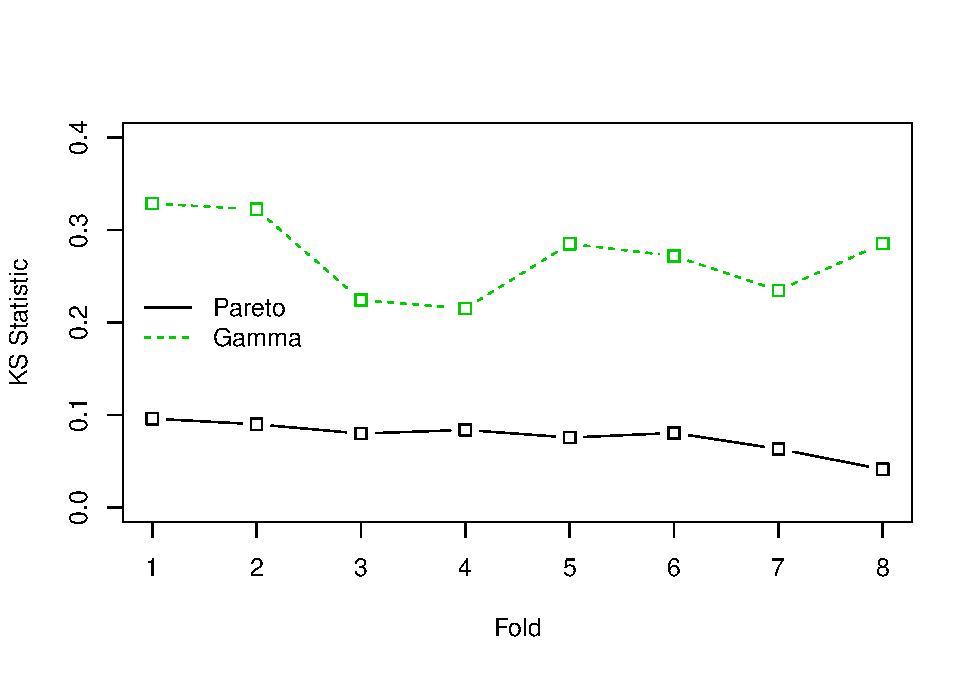
\includegraphics{LossDataAnalytics_files/figure-latex/KScvFig-1} 

}

\caption{Estadísticos de Kolmogorov-Smirnov (KS) con validación cruzada para los datos de siniestros del fondo de propiedad. La línea continua negra corresponde a la distribución de Pareto, la línea verde discontinua corresponde a la gamma. El estadístico KS mide la mayor desviación entre la distribución ajustada y la empírica para cada uno de los 8 grupos, o folds, de los datos seleccionados aleatoriamente.}\label{fig:KScvFig}
\end{figure}

\hypertarget{validaciuxf3n-cruzada-dejando-uno-fuera}{%
\subsection{Validación cruzada dejando uno fuera}\label{validaciuxf3n-cruzada-dejando-uno-fuera}}

El caso especial donde \(k=n\) es conocido como validación cruzada dejando uno fuera. Este caso tiene importancia históricamente y está muy relacionado con los estadísticos jackknife, un precursor de la técnica bootstrap.

A pesar de que se presenta como un caso especial de validación cruzada, es conveniente dar una definición explícita. Se considera un estadístico genérico \(\widehat{\theta}=t(\boldsymbol{x})\) que es un estimador del parámetro de interés \(\theta\). La idea de jackknife es calcular \(n\) valores \(\widehat{\theta}_{-i}=t(\boldsymbol{x}_{-i})\), donde \(\boldsymbol{x}_{-i}\) es una submuestra de \(\boldsymbol{x}\) con el \(i\)-ésimo valor eliminado. La media de esos valores se denota como

\[
\overline{\widehat{\theta}}_{(\cdot)}=\frac{1}{n}\sum_{i=1}^n \widehat{\theta}_{-i} .
\]
Esos valores pueden usarse para crear estimaciones del sesgo del estadístico \(\widehat{\theta}\)

\begin{equation}
Bias_{jack} = (n-1) \left(\overline{\widehat{\theta}}_{(\cdot)} - \widehat{\theta}\right)
\label{eq:Biasjack}
\end{equation}

así como de una estimación de la desviación estándar

\begin{equation}
s_{jack} =\sqrt{\frac{n-1}{n}\sum_{i=1}^n \left(\widehat{\theta}_{-i} -\overline{\widehat{\theta}}_{(\cdot)}\right)^2} ~.
\label{eq:sdjack}
\end{equation}

\textbf{Ejemplo 6.3.2. Coeficiente de variación.} A modo de ilustración, se considera una muestra pequeña ficticia \(\boldsymbol{x}=\{x_1,\ldots,x_n\}\) con realizaciones

\begin{verbatim}
sample_x <- c(2.46,2.80,3.28,3.86,2.85,3.67,3.37,3.40,
              5.22,2.55,2.79,4.50,3.37,2.88,1.44,2.56,2.00,2.07,2.19,1.77)
\end{verbatim}

Se desea determinar el coeficiente de variación
\(\theta = CV = \sqrt{\mathrm{Var~}X}/\mathrm{E~}X\).

Con esta base de datos, el estimador del coeficiente de variación resulta ser 0.31196. Pero, ¿cómo de fiable es este resultado? Para contestar a esta pregunta, se pueden calcular las estimaciones de jackknife del sesgo y su desviación estándar. El siguiente código muestra el estimador jackknife del sesgo es \(Bias_{jack} =\) -0.00627 y la desviación típica jackknife es \(s_{jack} =\) 0.01293.

\begin{center}\rule{0.5\linewidth}{0.5pt}\end{center}

\textbf{Ejemplo 6.3.3. Siniestros con daños corporales y ratios de eliminación de pérdida.} En el Ejemplo 6.2.1, se mostró como calcular estimaciones bootstrap del sesgo y desviación estándar para la ratio de eliminación de pérdidas usando los datos de siniestros con daños corporales del Ejemplo 4.1.11. Se continúa ahora proporcionando cuantías comparables usando los estadísticos jackknife.

\protect\hyperlink{tab:67}{Tabla 6.7} resume los resultados de la estimación jackknife. Muestra como la estimación jackknife del sesgo y la desviación estándar de la ratio de eliminación \(\mathrm{E}~\min(X,d)/\mathrm{E}~X\) son ampliamente consistentes con la metodología bootstrap. Es más, se pueden usar las desviaciones estándar para construir intervalos de confianza basados en la normal, centrados alrededor del estimador corregido por el sesgo. Por ejemplo, para \(d=14000\), se vio en el Ejemplo 4.1.11 que el estimador no paramétrico de \emph{LER} es 0.97678. Tiene un sesgo estimado de 0.00010, y resulta un estimador (jackknife) \emph{corregido por el sesgo} igual a 0.97688. Los intervalos de confianza al 95\% se obtienen creando un intervalo de dos veces la longitud de 1.96 desviaciones estándar jackknife, centrado sobre el estimador corregido por el sesgo (1.96 es aproximadamente el cuantil 97.5 de la distribución normal estándar).

\hypertarget{table-6.7.-estimaciones-jackknife-del-ler-en-las-franquicias-seleccionadas}{%
\paragraph*{Table 6.7. Estimaciones Jackknife del LER en las franquicias seleccionadas}\label{table-6.7.-estimaciones-jackknife-del-ler-en-las-franquicias-seleccionadas}}
\addcontentsline{toc}{paragraph}{Table 6.7. Estimaciones Jackknife del LER en las franquicias seleccionadas}

\begin{tabular}{r|r|r|r|r|r|r|r}
\hline
d & Estimación NP & Sesgo Bootstrap  & Bootstrap SD & Sesgo Jackknife  & Jackknife SD & Límite inferior del 95\% Jackknife CI & Límite superior del 95\% Jackknife CI\\
\hline
4000 & 0.54113 & 0.00011 & 0.01237 & 0.00031 & 0.00061 & 0.53993 & 0.54233\\
\hline
5000 & 0.64960 & 0.00027 & 0.01412 & 0.00033 & 0.00068 & 0.64825 & 0.65094\\
\hline
10500 & 0.93563 & 0.00004 & 0.01017 & 0.00019 & 0.00053 & 0.93460 & 0.93667\\
\hline
11500 & 0.95281 & -0.00003 & 0.00941 & 0.00016 & 0.00047 & 0.95189 & 0.95373\\
\hline
14000 & 0.97678 & 0.00016 & 0.00687 & 0.00010 & 0.00034 & 0.97612 & 0.97745\\
\hline
18500 & 0.99382 & 0.00014 & 0.00331 & 0.00003 & 0.00017 & 0.99350 & 0.99415\\
\hline
\end{tabular}

\begin{center}\rule{0.5\linewidth}{0.5pt}\end{center}

\textbf{Discusión.} Una de las cosas más interesantes sobre el caso especial de validación cruzada dejando uno fuera es la habilidad de replicar estimaciones de manera exacta. Es decir, cuando el tamaño del grupo o fold es solo uno, entonces no hay incertidumbre adicional inducida por la validación cruzada. Esto significa que los analistas pueden replicar de manera exacta el trabajo de otro, lo cual es una importante consideración.

Los estadísticos Jackknife fueron desarrollados para entender la precisión de estimadores, produciendo estimadores de sesgo y desviación estándar en las ecuaciones \eqref{eq:Biasjack} y \eqref{eq:sdjack}. Esto tiene que ver con algunas metas que se han asociado con las técnicas de bootstrap, no con métodos de validación cruzada. Esto demuestra como las técnicas estadísticas pueden usarse para alcanzar diferentes metas.

\hypertarget{validaciuxf3n-cruzada-y-bootstrap}{%
\subsection{Validación cruzada y Bootstrap}\label{validaciuxf3n-cruzada-y-bootstrap}}

El bootstrap es útil para proporcionar estimadores de la precisión, o variabilidad, de los estadísticos. También puede ser útil para la validación de modelos. El enfoque bootstrap para la validación de modelos es similar al enfoque dejando uno fuera y los procedimientos de validación \emph{k} fold:

\begin{itemize}
\tightlist
\item
  Se crea una muestra de bootstrap a través del remuestreo (con reemplazamiento) \(n\) índices en \(\{1,\cdots,n\}\). Esta será la \emph{muestra de entrenamiento}. Se estima el modelo considerado en base a esta muestra.
\item
  La muestra de \emph{prueba}, o \emph{muestra de validación}, consiste en esas observaciones no seleccionadas para en entrenamiento. Se evalúa el modelo ajustado (basado en los datos de entrenamiento) usando los datos de prueba.
\end{itemize}

Este proceso se repite muchas (digamos \(B\)) veces. Se toma la media de los resultados y se selecciona al modelo basado en el estadístico de evaluación promedio.

\textbf{Ejemplo 6.3.4. Fondo de propiedad de Wisconsin.} Se vuelve a considerar el ejemplo 6.3.1 donde se investiga el ajuste de unas distribuciones gamma y Pareto a los datos del fondo de propiedad. Nuevamente se compara el desempeño predictivo usando el estadístico de Kolmogorov-Smirnov pero esta vez usando el procedimiento bootstrap para partir los datos entre muestra de entrenamiento y prueba. A continuación, se muestra el código ilustrativo.

Se ha realizado el muestreo usando \(B=\) 100 réplicas. El estadístico \emph{KS} promedio de la distribución Pareto era 0.058, que puede compararse con el promedio para la distribución gamma, 0.262. Esto es consistente con los resultados anteriores y proporciona una evidencia más de que el modelo Pareto es mejor para estos datos que el gamma.

\hypertarget{S:ImportanceSampling}{%
\section{Importance Sampling}\label{S:ImportanceSampling}}

En la Sección \ref{S:SimulationFundamentals} se introducen las técnicas de Monte Carlo usando la técnica de la inversa: generar una variable aleatoria \(X\) con distribución \(F\), aplicar \(F^{-1}\) para llamar a un generador aleatorio (uniforme en el intervalo unitario). ¿Qué pasa si queremos realizar extracciones de acuerdo con \(X\), condicionado a \(X\in[a,b]\) ?

Se puede usar un mecanismo de aceptación-rechazo : extraer \(x\) de la distribución \(F\)

\begin{itemize}
\tightlist
\item
  si \(x\in[a,b]\) : se mantiene (``\emph{aceptación}'')
\item
  si \(x\notin[a,b]\) : se extrae otro (``\emph{rechazo}'')
\end{itemize}

Se observa que de \(n\) valores inicialmente generados, se mantienen sólo \([F(b)-F(a)]\cdot n\) extracciones, en promedio.

\textbf{Ejemplo 6.4.1. Extracciones de una distribución Normal.}\\
Supongamos que se realizan extracciones de una distribución normal con media 2.5 y varianza 1, \(N(2.5,1)\), pero sólo se tiene interés en extracciones en extracciones mayores que \(a \ge 2\) y menores que \(b \le 4\). Es decir, se puede usar sólo una proporción de extracciones igual a \(F(4)-F(2) = \Phi(4-2.5)-\Phi(2-2.5)\) = 0.9332 - 0.3085 = 0.6247. La Figura \ref{fig:sampleani1} demuestra que algunas extracciones caen en el intervalo \((2,4)\) y otras están fuera.

\begin{center}\rule{0.5\linewidth}{0.5pt}\end{center}

En su lugar, se pueden realizar extracciones de acuerdo con la distribución condicional \(F^{\star}\) definida como

\[
F^{\star}(x) = \Pr(X \le x | a < X \le b) =\frac{F(x)-F(a)}{F(b)-F(a)}, \ \  \ \text{for } a < x \le b .
\]
Usando el método de la transformada inversa de la Sección \ref{S:InverseTransform}, se tiene que la extracción

\[
X^\star=F^{\star-1}\left( U \right) = F^{-1}\left(F(a)+U\cdot[F(b)-F(a)]\right)
\]
tiene distribución \(F^{\star}\). Expresado de otra forma, se define

\[
\tilde{U} = (1-U)\cdot F(a)+U\cdot F(b)
\]
y entonces se usa \(F^{-1}(\tilde{U})\). Con este enfoque, cada extracción cuenta.

Esto puede estar relacionado con la importancia del mecanismo de muestreo : se realizan extracciones más frecuentemente en regiones donde se espera tener cantidades que tienen algún interés. Esta transformación puede ser considerada como ``un cambio de medida.''

En el Ejemplo 6.4.1., la inversa de la distribución normal está disponible fácilmente (en \texttt{R}, la función es \texttt{qnorm}). Sin embargo, para otras aplicaciones, este no es el caso. Entonces, simplemente se usan métodos numéricos para determinar \(X^\star\) como la solución de la ecuación \(F(X^\star) =\tilde{U}\) donde \(\tilde{U}=(1-U)\cdot F(a)+U\cdot F(b)\). Véase el siguiente código ilustrativo.

\hypertarget{S:MCMC}{%
\section{Monte Carlo Markov Chain (MCMC)}\label{S:MCMC}}

\begin{center}\rule{0.5\linewidth}{0.5pt}\end{center}

\textbf{Esta sección se está escribiendo y no está complete ni editada. El contenido que se muestra es para haceros una idea de lo que contendrá la versión final.}

\begin{center}\rule{0.5\linewidth}{0.5pt}\end{center}

La idea de las técnicas de Monte Carlo se basa en la ley de los grandes números (que asegura la convergencia de la media hacia la integral) y el teorema central del límite (que se usa para cuantificar la incertidumbre en los cálculos). Es necesario recordar que si \((X_i)\) es una secuencia i.id. de variables aleatorias con distribución \(F\), entonces

\[
\frac{1}{\sqrt{n}}\left(\sum_{i=1}^n h(X_i)-\int h(x)dF(x)\right)\overset{\mathcal{L}}{\rightarrow }\mathcal{N}(0,\sigma^2),\text{ as }n\rightarrow\infty.
\]
para alguna varianza \(\sigma^2>0\). Pero de hecho, el teorema ergódico se puede usar para rebajar el resultado anterior, dado que no es neceario tener independencia de las variables. Más concretamente, si \((X_i)\) es un proceso de Markov con medida invariante \(\mu\), bajo algunos supuestos técnicos adicionales, se puede obtener que

\[
\frac{1}{\sqrt{n}}\left(\sum_{i=1}^n h(X_i)-\int h(x)d\mu(x)\right)\overset{\mathcal{L}}{\rightarrow }\mathcal{N}(0,\sigma_\star^2),\text{ as }n\rightarrow\infty.
\]
para alguna varianza \(\sigma_\star^2>0\).

Por lo tanto, de esta propiedad, se puede ver que es posible no necesariamente generar valores independientes a partir de \(F\), sino también generar un proceso de markov con medida invariante \(F\), y considerar medias sobre el proceso (no necesariamente independiente).
Se considera el caso de un vector Gausiano restringido: se desean generar parejas aleatorias de un vector aleatorio \(\boldsymbol{X}\), pero sólo interesa el caso en que la suma de los (`composants')` es suficientemente grande, lo que puede expresarse como \(\boldsymbol{X}^T\boldsymbol{1}> m\) para algún valor real \(m\). Por supuesto, es posible usar el algoritmo \emph{aceptación-rechazo}, pero se ha vito que puede ser bastante ineficiente. Se puede usar el Hastings Metropolis y el muestreo de Gibbs para generar un proceso de Markov con esta medida invariante.

\hypertarget{hastings-metropolis}{%
\subsection{Hastings Metropolis}\label{hastings-metropolis}}

El algoritmo es bastante simple de generar a partir de \(f\): se comienza con un valor factible \(x_1\). Entonces, en el paso \(t\), se necesita especificar una transición núcleo: dado \(x_t\), se necesita la distribución condicional de \(X_{t+1}\) dado \(x_t\). El algoritmo funcionará bien si la distribución condicional se puede simular fácilmente. Sea \(\pi(\cdot|x_t)\) esta probabilidad.
Se obtiene un valor potencial \(x_{t+1}^\star\), y \(u\), de una distribución uniforme. Se calcula

\[
R=  \frac{f(x_{t+1}^\star)}{f(x_t)}
\]
y

\begin{itemize}
\tightlist
\item
  si \(u < r\), entonces \(x_{t+1}=x_t^\star\)
\item
  si \(u\leq r\), entonces \(x_{t+1}=x_t\)
\end{itemize}

Aquí \(r\) se denomina ratio-\emph{aceptación}: se acepta el nuevo valor con probabilidad \(r\) (o en realidad el menor entre \(1\) y \(r\) dado que \(r\) puede exceder \(1\)).

Por ejemplo, se asume que \(f(\cdot|x_t)\) es uniforme en \([x_t-\varepsilon,x_t+\varepsilon]\) para algún \(\varepsilon>0\), y donde \(f\) (la distribución objetivo) es la \(\mathcal{N}(0,1)\). Nunca se realizarán \emph{extracciones} de \(f\), pero se usará para calcular la ratio de aceptación en cada paso.

En el código de arriba, \texttt{vec} contiene los valores de \(\boldsymbol{x}=(x_1,x_2,\cdots)\), \texttt{innov} es la innovación.

Ahora, si se usan más simulaciones, se obtiene

\hypertarget{muestreo-de-gibbs}{%
\subsection{Muestreo de Gibbs}\label{muestreo-de-gibbs}}

Se considera algún vector \(\boldsymbol{X}=(X_1,\cdots,X_d)\) con components independientes, \(X_i\sim\mathcal{E}(\lambda_i)\). Se realiza un muestro para muestrear de \(\boldsymbol{X}\) dado \(\boldsymbol{X}^T\boldsymbol{1}>s\) para algún umbral \(s>0\).

\begin{itemize}
\tightlist
\item
  se comienza con algún valor inicial \(\boldsymbol{x}_0\) tal que
\item
  se elige (aleatoriamente) \(i\in\{1,\cdots,d\}\)
\item
  \(X_i\) dado que \(X_i > s-\boldsymbol{x}_{(-i)}^T\boldsymbol{1}\) tiene una distribucion Exponencial \(\mathcal{E}(\lambda_i)\)
\item
  se extrae \(Y\sim \mathcal{E}(\lambda_i)\) y se establece \(x_i=y +(s-\boldsymbol{x}_{(-i)}^T\boldsymbol{1})_+\) hasta que
  \(\boldsymbol{x}_{(-i)}^T\boldsymbol{1}+x_i>s\)
\end{itemize}

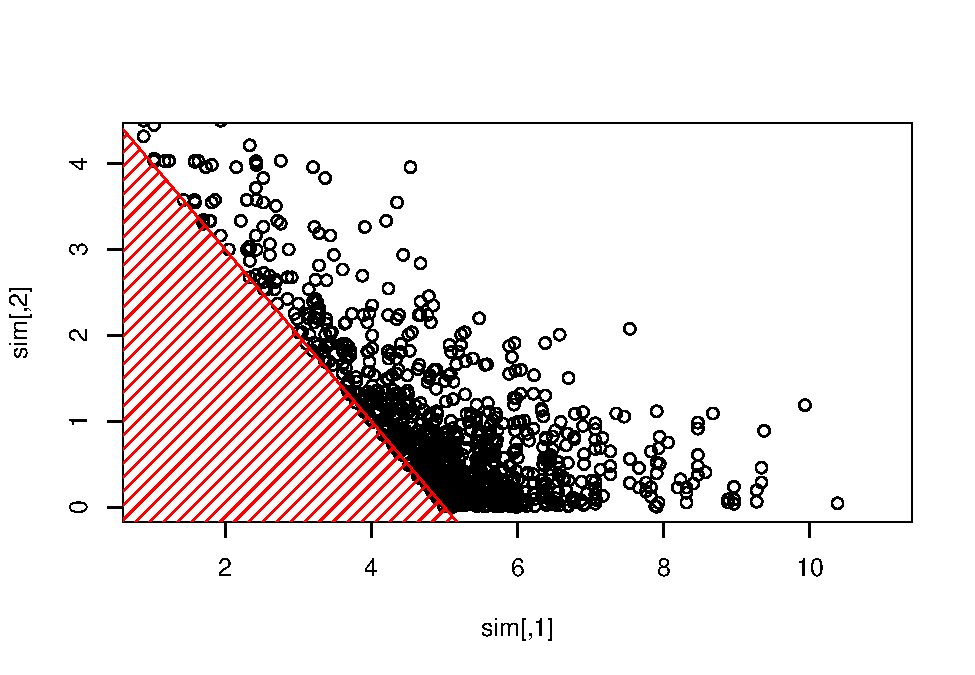
\includegraphics{LossDataAnalytics_files/figure-latex/unnamed-chunk-172-1.pdf}

La construcción de la secuencia (los algoritmos MCMC son iterativos) puede visualizarse abajo

\hypertarget{Simulation:further-reading-and-resources}{%
\section{Recursos Adicionales y Colaboradores}\label{Simulation:further-reading-and-resources}}

\begin{itemize}
\tightlist
\item
  Include historical references for jackknife (Quenouille, Tukey, Efron)
\item
  Aquí se muestran algunos links para aprender más sobre \href{https://freakonometrics.hypotheses.org/6470}{reproducibilidad y aleatoriedad} y cómo ir
  \href{https://freakonometrics.hypotheses.org/6638}{de un generador aleatorio a una función muestra}.
\end{itemize}

\hypertarget{colaboradores-3}{%
\subsubsection*{Colaboradores}\label{colaboradores-3}}
\addcontentsline{toc}{subsubsection}{Colaboradores}

\begin{itemize}
\tightlist
\item
  \textbf{Arthur Charpentier}, Université du Quebec á Montreal, y \textbf{Edward W. (Jed) Frees}, University of Wisconsin-Madison, son los principales autores de la versión inicial de este capítulo. Email: \href{mailto:jfrees@bus.wisc.edu}{\nolinkurl{jfrees@bus.wisc.edu}} y/o \href{mailto:arthur.charpentier@gmail.com}{\nolinkurl{arthur.charpentier@gmail.com}} para comentarios sobre este capítulo y sugerencias de mejora.
\item
  Revisores del capítulo: Escribir a Jed o Arthur; para añadir tu nombre aquí.
\item
  Traducción al español: Ana María Pérez-Marín (Universitat de Barcelona).
\end{itemize}

\hypertarget{ts-6.a.-bootstrap-applications-in-predictive-modeling}{%
\subsection{TS 6.A. Bootstrap Applications in Predictive Modeling}\label{ts-6.a.-bootstrap-applications-in-predictive-modeling}}

\begin{center}\rule{0.5\linewidth}{0.5pt}\end{center}

\textbf{This section is being written.}

\begin{center}\rule{0.5\linewidth}{0.5pt}\end{center}

\hypertarget{C:PremiumFoundations}{%
\chapter{Fundamentos de la Prima}\label{C:PremiumFoundations}}

\emph{Resumen del capítulo.} Definir los precios para los productos aseguradores, las primas, es una tarea importante para los actuarios y otros analistas de datos. Este capítulo introduce las bases o fundamentos para tarificar productos de no-vida.

\hypertarget{S:IntroductionRatemaking}{%
\section{Introducción a la Tarificación}\label{S:IntroductionRatemaking}}

\begin{center}\rule{0.5\linewidth}{0.5pt}\end{center}

En esta sección, se aprende cómo:

\begin{itemize}
\tightlist
\item
  Definir la esperanza matemática como referencia del método para determinar las primas del seguro
\item
  Analizar una ecuación contable para relacionar primas con siniestros, gastos y beneficios
\item
  Resumir la estrategia para extender la tarificación en caso de riesgos heterogéneos y tendencias temporales
\end{itemize}

\begin{center}\rule{0.5\linewidth}{0.5pt}\end{center}

Este capítulo explica cómo podemos pensar en determinar el precio apropiado para un producto asegurador. Como se describe en la Sección \ref{S:PredModApps}, una función actuarial clave es la tarificación, donde el analista busca determinar el precio correcto para un riesgo.

Siendo ésta una función clave, empecemos por dar un paso atrás y definir algunos términos. Un precio es una cantidad, normalmente de dinero, que es intercambiada por un producto o un servicio. En seguros, normalmente utilizamos la palabra prima como la cantidad de dinero cobrada por la protección aseguradora ante acontecimientos inciertos. La cantidad de protección varía según el riesgo asegurado. Por ejemplo, en un seguro del hogar, la cantidad de la protección del seguro depende del valor de la casa. En un seguro de vida, la cantidad de protección depende del estado financiero (p.~ej. ingresos y riqueza) del asegurado, así como de la necesidad percibida para su seguridad financiera. En consecuencia, es común expresar el precio del seguro como una unidad de la protección que está siendo adquirida, por ejemplo, una cantidad en miles (p.~ej., de dólares o Euros) para la cobertura de una casa o del pago acordado en caso de muerte. Como estos/as precios/primas están expresados/as en unidades estandarizadas, también se denominan como tarifas.

Para determinar precios, en economía, es común considerar la oferta y la demanda de un producto. La demanda es sensible al precio y a la existencia de empresas en competencia o de productos alternativos. La oferta viene determinada en función de los recursos necesarios para la producción. Para una empresa individual, el precio estará definido para cumplir con el objetivo de maximizar su beneficio, lo que conseguirá escogiendo el nivel de producción que equilibre los costes y los ingresos al nivel de margen deseado.

Sin embargo, una peculiaridad del seguro es que los costes de la protección aseguradora no son conocidos en el momento de la venta del contrato. Si el acontecimiento incierto asegurado, como la pérdida de una casa o la vida, no ocurre, entonces los costes de contrato son sólo administrativos (para formalizar el contrato) y son relativamente menores. Si el acontecimiento asegurado ocurre, entonces el coste incluye no sólo los costes administrativos sino también el pago de la cantidad asegurada y los gastos para gestionar la reclamación. Por lo tanto, el coste es aleatorio cuando el contrato se formaliza: por diseño del producto, ni asegurador ni asegurado conocen los costes de contrato. Además, los costes pueden no ser revelados en meses o años. Por ejemplo, un tiempo normal para la liquidación de una mala práctica médica es de cinco años.

Al ser desconocidos los costes en el momento de la venta, la determinación del precio del seguro difiere de las aproximaciones económicas comunes.

Este capítulo aborda decididamente la naturaleza incierta de los costes mediante aproximaciones actuariales tradicionales que determinan los precios en función de los costes del seguro. Como veremos, esta aproximación de tarificación es suficiente para algunos ramos de seguro, como automóvil o hogar, donde el asegurador tiene una cartera de muchos riesgos independientes. Sin embargo, existen otros ramos de seguro donde los precios actuariales sólo proporcionan un dato más para los precios generales del mercado. Para reforzar esta distinción, las primas basadas en el coste actuarial son a veces denominadas como precios técnicos. Desde la perspectiva de los economistas, algunas decisiones corporativas como la tarificación deben ser evaluadas teniendo en cuenta su impacto en el valor de mercado de la empresa. Este objetivo es más completo que la idea estática de la maximización del beneficio. Esto es, asumiendo que el valor de la empresa representa el valor actualizado de todos los beneficios esperados en el futuro. Las decisiones que impactan en este valor afectan a todos aquellos grupos que pueden reclamar a la empresa, incluyendo accionistas, obligacionistas, asegurados (en el caso de las mutuas de seguros), y otros.

\textless!---Dado que los costes no son conocidos en el momento de la venta del seguro, este capítulo se centra, siguiendo la literatura actuarial, en los costes de ofrecer un seguro. Esta no será una visión completa de todo lo necesario para determinar el precio del seguro. --\textgreater{}

Para los precios basados en costes, es útil pensar en la prima como fuente de ingresos necesaria para hacer frente a los pagos de los siniestros y los gastos operativos, y además, obtener un margen de beneficio. Podemos formalizar esto en la siguiente ecuación contable

\begin{equation}
\small{
\text{Prima = Siniestros + Gastos + Margen Beneficio} .
}
\label{eq:AccountingEquation}
\end{equation}

Los gastos pueden ser divididos entre aquellos que varían según la prima (como las comisiones por ventas) y los que no (como los costes de gestión y los salarios de los empleados). El término \texttt{Margen\ Beneficio} es la parte residual que representa el beneficio por suscripción (underwriting benefit, en inglés). También puede incluir el coste de capital (por ejemplo, el dividendo anual a los inversores de la compañía). Como estos gastos fijos y costes de capitales son difícilmente interpretables al nivel de los contratos individuales, pensamos en la igualdad de la ecuación \eqref{eq:AccountingEquation} como aquella existente sobre la suma de muchos contratos (una cartera) y trabajamos con ella a nivel agregado o \emph{conjunto}. De este modo, en la Sección \ref{S:AggRateMaking} utilizamos esta aproximación para ayudarnos a determinar aproximadamente las primas, por ejemplo, fijando objetivos de beneficio. Específicamente, en las secciones \ref{S:PurePremium} y \ref{S:LossRatio}, introducimos los dos métodos predominantes en la práctica para determinar primas, el método de la prima pura y el del ratio de siniestralidad.

Los \texttt{Siniestros} en la ecuación \eqref{eq:AccountingEquation} son aleatorios y por tanto, como referencia, utilizamos los \emph{costes esperados} para determinar las tarifas. Existen diferentes maneras de argumentar esta perspectiva que ampliaremos en la Sección \ref{S:PricingPrinciples}. Por ahora, supondremos que el asegurador suscribe muchos contratos con riesgos similares, excepto que, por pura casualidad, en algunos casos el acontecimiento asegurado ocurre y en otros no. El asegurador se obliga a pagar la cantidad total de reclamaciones por siniestros de todos sus contratos. Si los riesgos son similares, entonces todos los asegurados deberían aportar la misma cantidad, que sería el pago medio por siniestro. Desde esta perspectiva, tiene sentido focalizarnos en el pago medio de los siniestros de un conjunto de asegurados. De la teoría de la probabilidad, específicamente de la ley de los grandes números, sabemos que la media de riesgos iid se aproxima a la cantidad esperada, por lo que podemos utilizar la esperanza matemática como un principio básico de tarificación.

No obstante, utilizando la siniestralidad esperada, esencialmente suponemos que la incertidumbre es inexistente. Si los aseguradores suscriben suficientes pólizas independientes, ésta puede ser una aproximación razonable. Sin embargo, habrá otros casos, como en un contrato único para una gran empresa en el que se aseguran todos sus edificios por incendio, donde el uso exclusivo de una esperanza matemática para tarificar no será suficiente. Por esta razón, en la Sección \ref{S:PricingPrinciples}, también resumiremos los principios alternativos de tarificación que incorporan la incertidumbre a nuestra fijación de precios. Nótese que un especial énfasis de este texto es la estimación de la distribución entera de la siniestralidad para que el analista no se vea restringido a trabajar sólo con la esperanza matemática.

Los métodos de tarificación conjuntos derivados de la ecuación \eqref{eq:AccountingEquation} se centran en colecciones de riesgos homogéneos que son similares excepto por la ocurrencia o no de siniestros aleatorios. En el lenguaje estadístico que hemos introducido, esto es una discusión sobre si los riesgos presentan distribuciones idénticas o no. Por supuesto, cuando examinamos los riesgos suscritos por los aseguradores, encontramos muchas variaciones en los riesgos asegurados, incluyendo las características de los contratos y de las personas aseguradas. En la Sección \ref{S:HeterogeneousRisks} extendemos las consideraciones de tarificación para colecciones de riesgos heterogéneos.

En la Sección \ref{S:TrendDevelopment} introducimos algunas ideas sobre desarrollo y tendencia. Cuando tarificamos, queremos utilizar la experiencia de siniestralidad más reciente porque el objetivo es definir tarifas con una visión prospectiva. Sin embargo, al inicio de un contrato, la experiencia de siniestralidad reciente es a menudo desconocida; pueden pasar varios años hasta que se produzca completamente. Por esta razón, en esta sección, se introducen los conceptos necesarios para incorporar la experiencia de siniestralidad reciente en el desarrollo de nuestra prima. Desarrollo y tendencia de la experiencia de siniestralidad está relacionada, pero también difiere, de la idea de la tarificación basada en la experiencia que sugiere que la experiencia revela información no disponible a priori sobre el asegurado y que tendría que ser incorporada en consonancia con nuestro punto de vista prospectivo. El Capítulo \ref{C:Credibility} presenta esta idea con más detalle.

La sección final de este capítulo introduce métodos para seleccionar una prima. Esto será realizado mediante la comparación entre un método de tarificación y la siniestralidad de la cartera analizada y seleccionando el método que produce un mejor ajuste con los datos analizados. Para una cartera de seguros típica, la mayoría de pólizas no declaran siniestros, esto es, no comportan pérdidas. Como la distribución de los siniestros analizados es una combinación de (un número grande de) ceros y cantidades continuas, técnicas especiales serán útiles aquí. La Sección \ref{S:GiniStatistic} introduce los conceptos de \emph{curvas de concentración} y los correspondientes \emph{estadísticos de Gini} para ayudar en esta selección.

El capítulo también incluye un suplemento técnico sobre la regulación gubernamental referente a las tarifas del seguro para mantener nuestro trabajo en el marco de las aplicaciones reales.

\hypertarget{S:AggRateMaking}{%
\section{Métodos de Tarificación Conjunta}\label{S:AggRateMaking}}

\begin{center}\rule{0.5\linewidth}{0.5pt}\end{center}

En esta sección, se aprende cómo:

\begin{itemize}
\tightlist
\item
  Definir una prima pura como un coste de siniestralidad, tanto en términos de frecuencia como de severidad
\item
  Calcular una tarifa específica utilizando primas puras, gastos, y márgenes de beneficio
\item
  Definir una ratio de siniestralidad (loss ratio, en inglés)
\item
  Calcular un cambio de tarifa específica utilizando ratios de siniestralidad
\item
  Comparar los métodos de prima pura y de ratio de siniestralidad para determinar primas
\end{itemize}

\begin{center}\rule{0.5\linewidth}{0.5pt}\end{center}

Es común considerar la experiencia conjunta de una cartera de seguros. Compatible con la notación anterior, consideramos una colección de \emph{n} contratos con siniestros \(X_1, \ldots, X_n\). En esta sección, suponemos que los contratos tienen la misma distribución de siniestralidad, en otras palabras forman una cartera homogénea, y, por tanto, son iid. Como justificación, podemos pensar en un seguro personal como el de automóvil o hogar, donde los aseguradores suscriben muchos contratos de riesgos muy similares. En tal caso, la suposición de distribuciones idénticas no es tan limitativa como podríamos pensar en un principio. En la Sección \ref{S:ExposureToRisk} introduciremos la idea de una exposición variable que nos permitirá rescalar la experiencia de siniestralidad para hacerla comparable. Por ejemplo, rescalando los siniestros seremos capaces de tratar los siniestros de hogar de una casa de 100.000 y los de una casa de 200.000 como pertenecientes a una misma distribución. Por ahora, sencillamente suponemos que \(X_1, \ldots, X_n\) son \emph{iid}.

\hypertarget{S:PurePremium}{%
\subsection{Método de la Prima Pura}\label{S:PurePremium}}

Si el número en el grupo, \emph{n}, es grande, entonces la media proporciona una buena aproximación de la siniestralidad esperada

\[
\small{
\mathrm{E}(X) \approx \frac{\sum_{i=1}^n X_i}{n} = \frac{\text{Siniestralidad}}{\text{Exposición}} = \text{Prima Pura}.
}
\]

Con este enfoque, definimos la prima pura como la suma de los siniestros dividida por la exposición; y que también es conocida como coste de siniestralidad. En el caso de riesgos homogéneos, todas las pólizas son tratadas igual y podemos utilizar el número de pólizas \emph{n} para la exposición. En la Sección \ref{S:ExposureToRisk} extendemos el concepto de exposición cuando las pólizas no son iguales.

Podemos multiplicar y dividir por el número de reclamaciones, \texttt{claim\ count} en inglés, para conseguir

\[
\small{
\text{Prima Pura} = \frac{\text{número de reclamaciones}}{\text{Exposición}} \times \frac{\text{Siniestralidad}}{\text{número de reclamaciones}} = \text{frecuencia} \times \text{severidad} .
}
\]

Por lo tanto, cuando calculamos las primas utilizando el método de la prima pura, podemos considerar tanto la siniestralidad media (coste de siniestralidad) como la aproximación frecuencia-severidad.

Para conseguir estar más cerca de las aplicaciones prácticas, volvemos ahora a la ecuación \eqref{eq:AccountingEquation} que también incluye los gastos. La ecuación \eqref{eq:AccountingEquation} también se refiere al \texttt{Margen\ de\ beneficio} para incluir el beneficio de suscripción. Si éste lo relacionamos con las primas, lo denominaremos recargo de beneficio. Como los siniestros son inciertos, el asegurador debe disponer de capital suficiente para asegurar que todas las reclamaciones serán pagadas. Mantener este capital extra es un coste del propio negocio, los inversores de la compañía deben ser compensados por ello, de ahí el recargo extra.

A continuación, descomponemos los \texttt{Gastos} en aquellos que varían según la prima, \texttt{Variables}, y los que no, \texttt{Fijos} de modo que \texttt{Gastos\ =\ Variables\ +\ Fijos}. Pensando en los gastos variables y los beneficios como una fracción de las primas, definimos

\[
\small{
V =  \frac{\text{Variables}}{\text{Prima}} ~~~ \text{y}~~~
Q = \frac{\text{Margen de beneficio}}{\text{Prima}} ~.
}
\]

Con estas definiciones y la ecuación \eqref{eq:AccountingEquation}, podemos escribir

\[
\small{
\begin{matrix}
\begin{array}{ll}
\text{Prima} &= \text{Siniestros + Fijos} + \text{Prima} \times \frac{\text{Variables + Margen de beneficio }}{\text{Prima}}  \\
& = \text{Siniestros + Fijos} + \text{Prima} \times (V+Q) .
\end{array}
\end{matrix}
}
\]

Despejando

\begin{equation}
\small{
\text{Prima} = \frac{\text{Siniestros + Fijos}}{1-V-Q} .
}
\label{eq:PremiumEquation}
\end{equation}

Dividiendo por la exposición, la tarifa puede ser calculada como

\[
\begin{matrix}
\begin{array}{ll}
\text{Tarifa} &= \frac{\text{Prima}}{\text{Exposición}} = \frac{\text{Siniestros/Exposición + Fijos/Exposición}}{1-V-Q} \\
&=   \frac{\text{Prima pura + Fijos/Exposición}}{1-V-Q} ~.
\end{array}
\end{matrix}
\]

En otros términos, esto es

\[
\small{
\text{Tarifa} =\frac{\text{prima pura + gastos fijos por exposición }}{\text{1 – factor de gastos variables – factor de beneficio y contingencias}}  .
}
\]

\textbf{Ejemplo. CAS Examen 5, 2004, Número 13.} Determinar la tarifa de referencia por unidad de exposición, dada la información siguiente:

\begin{itemize}
\tightlist
\item
  Frecuencia por unidad de exposición = 0,25
\item
  Severidad = \$100
\item
  Gasto fijo por unidad de exposición = \$10
\item
  Factor de gasto variable = 20\%
\item
  Factor de beneficio y contingencias = 5\%
\end{itemize}

\textbf{Solución.} Bajo el método de la prima pura, la tarifa de referencia es

\[
\begin{matrix}
\begin{array}{ll}
\text{Tarifa} &=  \frac{\text{prima pura + gastos fijos por exposición}}{\text{1 – factor de gastos variables – factor de beneficio y contingencias}}\\
&= \frac{\text{frecuencia} \times \text{severidad} ~+~10}{1-0,20-0,05} = \frac{0,25 \times 100 +10}{1-0,20-0,05} = 46,67.
\end{array}
\end{matrix}
\]

\begin{center}\rule{0.5\linewidth}{0.5pt}\end{center}

Del ejemplo, nótese que las tarifas calculadas por el método de la prima pura son generalmente denominadas como \emph{tarifa de referencia }.

De nuestra exposición, nótese también que el beneficio está asociado con aspectos de la suscripción y no con inversiones. Las primas son habitualmente pagadas al principio del contrato por lo que los aseguradores reciben ingresos por la inversión de este dinero. Sin embargo, debido a la naturaleza a corto plazo de estos contratos, los ingresos por la inversión son normalmente ignorados al tarificar. Esto aporta un poco de conservadurismo al proceso, lo que es bien recibido por los aseguradores. Probablemente esto es más relevante en ramos de cola muy larga, como el de accidentes laborales o el de malas prácticas médicas. En estos ramos, a veces pueden pasar 20 años, o incluso más, para resolver las reclamaciones. Pero estos ramos son también los más volátiles; los pagos de siniestros en un futuro lejano son menos extremos cuando se ven desde la perspectiva del descuento financiero.

\hypertarget{S:LossRatio}{%
\subsection{Método de la Ratio de Siniestralidad}\label{S:LossRatio}}

La ratio de siniestralidad (loss ratio, en inglés) es el cociente entre la suma de los siniestros y la prima

\[
\small{
\mathrm{E}(X) \approx \frac{\sum_{i=1}^n X_i}{n} = \frac{\text{Siniestralidad}}{\text{Exposición}} = \text{Prima Pura}.
}
\]

Cuando calculamos primas, es un poco contra intuitivo focalizarnos en esta ratio porque la componente prima está incorporada en su denominador. Como veremos, la idea es que el método de ratio de siniestralidad proporciona \textbf{cambios} de tarifa más que tarifas en sí; podemos utilizar cambios de tarifa para actualizar la experiencia pasada y así determinar la tarifa actual. Para hacer esto, los cambios de tarifa consisten en la ratio entre la ratio de siniestralidad observada y la ratio de siniestralidad objetivo. Este factor de ajuste es entonces aplicado a las tarifas actuales para conseguir las nuevas tarifas.

Para ver cómo esto funciona en un contexto sencillo, volvemos a la ecuación \eqref{eq:AccountingEquation} pero ahora ignorando los gastos: \(\small{\text{Prima = Siniestros + Margen Beneficio}}\). Dividiendo por la prima

\[
\small{
\frac{\text{Margen Beneficio}}{\text{Prima}} = 1 - RS = 1 - \frac{\text{Siniestralidad}}{\text{Prima}} .
}
\]

Supongamos que tenemos un nuevo ``objetivo'' del recargo de beneficio, \(Q_{objetivo}\). Suponiendo que los siniestros, la exposición, y otros elementos se mantienen igual, entonces para conseguir el nuevo objetivo de beneficio debemos ajustar la prima. Usamos \emph{FC} como el factor de cambio que está definido según la expresión

\[
\small{
\frac{\text{nuevo Margen Beneficio}}{\text{Prima}} = Q_{objetivo} =  1 - \frac{\text{Siniestralidad}}{FC \times \text{Prima}}.
}
\]

Despejando para \emph{FC}, obtenemos

\[
\small{
FC = \frac{\text{Siniestralidad}}{\text{Prima} \times (1-Q_{objetivo})} = \frac{RS}{1-Q_{objetivo}}.
}
\]

Por ejemplo, si tenemos un ratio de siniestralidad actual = 85\% y un objetivo de recargo de beneficio \(\small{Q_{objetivo}=0,20}\), entonces \(\small{FC = 0,85/0,80 = 1,0625}\), lo que significa que aumentamos primas en un 6,25\%.

Ahora veamos cómo funciona incluyendo los gastos en la ecuación \eqref{eq:AccountingEquation}. Podemos utilizar el mismo planteamiento que en la Sección \ref{S:PurePremium} e iniciar con la ecuación \eqref{eq:PremiumEquation} y despejando por el recargo de beneficio

\[
\small{
Q = 1 - \frac{\text{Siniestralidad+Fijos}}{\text{Prima}} - V .
}
\]
Interpretamos la cantidad \texttt{Fijos/Prima\ +\ V} como la ``ratio de gastos operacionales.'' Y ahora, fijamos un porcentaje de beneficio \emph{Q} como objetivo y ajustamos las primas según el ``factor de cambio'' \(FC\)

\[
\small{
Q_{objetivo} = 1
-\frac{\text{Siniestralidad+Fijos}}{\text{Prima}\times FC} - V .
}
\]

Despejando para \(FC\)

\begin{equation}
\small{
FC = \frac{\text{Siniestralidad+Fijos}}{\text{Prima} \times (1 - V - Q_{objetivo})}.
}
\label{eq:IndicatedChangeFactor}
\end{equation}

\textbf{Ejemplo. Factor de Cambio de Ratio de Siniestralidad.} Suponemos la información siguiente:

\begin{itemize}
\tightlist
\item
  Ratio de siniestralidad proyectado = 65\%
\item
  Ratio de gastos fijos proyectados = 6,5\%
\item
  Gastos variables = 25\%
\item
  Margen Beneficio objetivo = 10\%
\end{itemize}

Con estos supuestos y la ecuación \eqref{eq:IndicatedChangeFactor}, el factor de cambio puede ser calculado como

\[
\small{
FC = \frac{\text{(Siniestralidad+Fijos)}/\text{Prima}}{1 - V - Q_{objetivo}} = \frac{0,65 + 0,065}{1- 0,25 – 0,10} = 1,10.
}
\]

Esto significa que el nivel general de la tarifa tendría que ser aumentado en un 10\%.

\begin{center}\rule{0.5\linewidth}{0.5pt}\end{center}

Más adelante, en la Sección \ref{S:CompareMethods}, proporcionaremos una comparación entre los métodos de prima pura y ratio de siniestralidad. Como avance, esta sección requerirá los conocimientos sobre exposiciones, tendencias y primas definidos en la Sección \ref{S:TrendDevelopment}.

\hypertarget{S:PricingPrinciples}{%
\section{Principios de Tarificación}\label{S:PricingPrinciples}}

\begin{center}\rule{0.5\linewidth}{0.5pt}\end{center}

En esta sección, se aprende cómo:

\begin{itemize}
\tightlist
\item
  Describir los principios actuariales de tarificación más comunes
\item
  Describir las propiedades de los principios de tarificación
\item
  Escoger un principio de tarificación basándose en una propiedad deseada
\end{itemize}

\begin{center}\rule{0.5\linewidth}{0.5pt}\end{center}

Existen diferentes aproximaciones para la tarificación según el tipo de contrato. Por ejemplo, el seguro de automóvil para particulares es conocido como una parte importante del mercado minorista de seguros generales en el Reino Unido. En este caso, podemos esperar realizar la tarificación basándonos en un conjunto grande de contratos independientes, una situación en la que las esperanzas matemáticas de los siniestros proporcionan un punto de partida excelente. Por el contrario, un actuario puede tener que tarificar un contrato de seguro para un gran empresario que desea cubrir los complejos beneficios de salud para miles de empleados. En tal caso, el conocimiento de la distribución entera de los siniestros potenciales, no tan solo su valor esperado, es crucial para empezar las negociaciones de la tarifa. Para cubrir una gran gama de potenciales aplicaciones, en esta sección se describen los principales principios de tarificación y sus propiedades, que pueden utilizarse para decidir qué principio en concreto es aplicable en una situación determinada.

\hypertarget{principios-de-tarificaciuxf3n}{%
\subsection{Principios de Tarificación}\label{principios-de-tarificaciuxf3n}}

Este capítulo introduce los tradicionales principios de tarificación actuariales basados tan solo en la distribución de la siniestralidad; el precio no depende de la demanda de seguros u otros aspectos de los costes como los gastos. Suponemos que la siniestralidad \(X\) tiene una función de distribución \(F(\cdot)\) y que existen algunas funciones \(H\) que retorna \(F(\cdot)\) en la línea real positiva, denotado como \(P = H(F)\). Para propósitos de notación, es a menudo conveniente sustituir la variable aleatoria \(X\) por su función de distribución y escribir \(P = H(X)\). La tabla \ref{tab:PremPrinciples} proporciona varios ejemplos.

\begin{longtable}[]{@{}ll@{}}
\caption{\label{tab:PremPrinciples} Principios comunes de tarificación}\tabularnewline
\toprule
Descripción & Definición (\(H(X)\)) \\
\midrule
\endfirsthead
\toprule
Descripción & Definición (\(H(X)\)) \\
\midrule
\endhead
Prima neta (pura) & \(E[X]\) \\
Valor esperado & \((1+\alpha)E[X]\) \\
Desviación estándar & \(E[X]+\alpha SD(X)\) \\
Varianza & \(E[X]+\alpha Var(X)\) \\
Utilidad cero & Solución de \(u(w) = E u(w + P - X)\) \\
Exponencial & \(\frac{1}{\alpha} \ln E e^{\alpha X}\) \\
\bottomrule
\end{longtable}

Un principio de tarificación es similar a una medida de riesgo como las introducidas en la Sección \ref{S:RiskMeasure}. Matemáticamente, en ambos casos, son funciones que convierten la variable aleatoria (rv) de siniestralidad de interés en un valor numérico. Desde un punto de vista práctico, un principio de tarificación proporciona una guía de qué cantidad cobrará un asegurador para aceptar un riesgo \(X\). En cambio, una medida de riesgo cuantifica el nivel de incertidumbre, o riskiness en inglés, que un asegurador puede utilizar para decidir un nivel de capital suficiente para asegurar su solvencia.

Como se aprecia en la Tabla, la prima neta, o pura, esencialmente supone que no existe incertidumbre. Los principios del valor esperado, la desviación estándar y la varianza añaden un recargo explícito para la incertidumbre a través del parámetro \(\alpha \ge 0\). Para el principio de utilidad cero, pensamos en un asegurador con función de utilidad \(u(\cdot)\) y riqueza \emph{w} al que le resulta indiferente aceptar o no aceptar el riesgo \(X\). En este caso, \(P\) es conocido como el precio de indiferencia o, en economía, como precio de reserva. Con la utilidad exponencial, el principio de utilidad cero se reduce al principio de tarificación exponencial, esto es, suponiendo \(u(x) = (1-e^{-\alpha x})/\alpha\).

Para valores pequeños de los parámetros de riesgo, el principio de varianza es aproximadamente igual al principio exponencial, como se ilustra en el siguiente caso especial.

\begin{center}\rule{0.5\linewidth}{0.5pt}\end{center}

\textbf{Caso especial: Distribución Gamma }. Consideramos una siniestralidad distribuida como una gamma con parámetros \(\alpha\) y \(\theta\). Del Apéndice D en \ref{C:SummaryDistributions}, la media es \(\alpha \theta\) y la varianza es \(\alpha \theta^2\). Utilizando \(\alpha_{Var}\) como parámetro de riesgo, el principio de varianza es \(H_{Var}(X) = \alpha \theta+\alpha_{Var} (\alpha \theta^2)\). Del mismo apéndice, es directo derivar la función generadora de momentos, \(M(t) = E e^{tX} = (1-t\theta)^{-\alpha}\). Con esto y un parámetro de riesgo \(\alpha_{Exp}\), podemos expresar el principio exponencial como

\[
H_{Exp}(X) = \frac{-\alpha}{\alpha_{Exp}} \ln\left(1-\alpha_{Exp} \theta\right).
\]

Para ver la relación entre \(H_{Var}(X)\) y \(H_{Exp}(X)\), escogemos \(\alpha_{Exp} = 2 \alpha_{Var}\). Con una aproximación de cálculo (\(\ln(1-x) = -x - x^2/2 - x^3/3 - \cdots\)), podemos escribir

\[
H_{Exp}(X) = \frac{-\alpha}{\alpha_{Exp}} \ln\left(1-\alpha_{Exp} \theta\right) 
= \frac{-\alpha}{\alpha_{Exp}} \left\{ -\alpha_{Exp} \theta -(\alpha_{Exp} \theta)^2/2 - \cdots\right\} \\
\approx \alpha \theta + \frac{\alpha_{Exp}}{2}(\alpha \theta^2 ) 
= H_{Var}(X). 
\]

\hypertarget{propiedades-de-los-principios-de-tarificaciuxf3n}{%
\subsection{Propiedades de los Principios de Tarificación}\label{propiedades-de-los-principios-de-tarificaciuxf3n}}

Las propiedades de los principios de tarificación nos ayudan como guía en la selección de un principio de tarificación en las aplicaciones prácticas. La Tabla \ref{tab:Properties} proporciona algunos ejemplos de las propiedades de estos principios.

\begin{longtable}[]{@{}ll@{}}
\caption{\label{tab:Properties} Propiedades Comunes de los Principios de Tarificación}\tabularnewline
\toprule
Descripción & Definición \\
\midrule
\endfirsthead
\toprule
Descripción & Definición \\
\midrule
\endhead
Recargo no negativo & \(H(X) \ge E[X]\) \\
Aditividad & \(H(X_1+X_2) = H(X_1) + H(X_2)\), para \(X_1, X_2\) independientes \\
Invariancia de escala & \(H(cX) = c H(X)\), para \(c \ge 0\) \\
Consistencia & \(H(c+X) = c + H(X)\) \\
Acotabilidad & \(H(X) \le max ~range ~\{X\}\) \\
\bottomrule
\end{longtable}

Esta tabla es sencillamente un subconjunto de las muchas propiedades citadas en la literatura actuarial. Por ejemplo, el artículo de \citet{young2014premium} lista 15 propiedades. Véase también las propiedades descritas como \emph{axiomas coherentes} que introducimos para las medidas de riesgo en la Sección \ref{S:RiskMeasure}.

Algunas de las propiedades listadas en la Tabla \ref{tab:Properties} son suaves en el sentido que casi siempre serán satisfechas. Por ejemplo, la propiedad de \emph{acotabilidad} indica que el recargo de la prima será más pequeño que el valor máximo de la siniestralidad \(X\). Otras propiedades pueden no ser tan suaves. Por ejemplo, para una cartera de riesgos independientes, el actuario puede querer que se cumpla la propiedad de \emph{aditividad}. Es fácil ver que esta propiedad se cumple para los principios del valor esperado, varianza, y exponencial, pero no para el principio de desviación estándar. Otro ejemplo es la propiedad de \emph{consistencia} que no se cumple para el principio de valor esperado cuándo el parámetro de riesgo del recargo \(\alpha\) es positivo.

El principio de \emph{invariancia de escala} es conocido como \emph{homogeneidad de grado uno} en economía. Nos permite, por ejemplo, trabajar con monedas diferentes (p.~ej., de dólares a Euros), así como en otras aplicaciones que serán comentadas más adelante en la Sección siguiente \ref{S:HeterogeneousRisks}. A pesar de que es un principio generalmente aceptado, nótese que este principio no se cumple para unos valores grandes de \(X\) que pueden limitar los beneficios de un asegurador; si un asegurador tiene una probabilidad elevada de devenir insolvente, entonces el asegurador no deseará utilizar un criterio lineal de tarificación. Es fácil comprobar que este principio se cumple para los principios del valor esperado y desviación estándar, pero no para los principios de varianza y exponencial.

\hypertarget{S:HeterogeneousRisks}{%
\section{Riesgos Heterogéneos}\label{S:HeterogeneousRisks}}

\begin{center}\rule{0.5\linewidth}{0.5pt}\end{center}

En esta sección, se aprende cómo:

\begin{itemize}
\tightlist
\item
  Describir exposiciones de seguro en términos de escala de distribuciones
\item
  Explicar una exposición en términos de algunos tipos de seguro comunes, como los seguros de automóvil y hogar
\item
  Describir cómo los factores de tarificación pueden utilizarse para tener en cuenta la heterogeneidad entre los riesgos de una cartera
\item
  Medir el impacto de los factores de tarificación mediante relatividades
\end{itemize}

\begin{center}\rule{0.5\linewidth}{0.5pt}\end{center}

Como se apuntó en la Sección \ref{S:IntroductionRatemaking}, hay mucha variabilidad en los riesgos que son asegurados, las características de los contratos, y en las personas aseguradas. Como ejemplo, podríamos tener un hermano o hermana gemelo que trabaja en la misma ciudad y gana una cantidad similar de dinero. Aún así, cuando llegara el momento de seleccionar opciones en el seguro de alquiler que cubriera los contenidos de nuestros apartamentos, nos podemos imaginar que existirían diferencias en la cantidad de contenidos asegurables, en las elecciones de las franquicias para definir la cantidad retenida, y quizás niveles diferentes de incertidumbre según la seguridad relativa de nuestros barrios. Las personas y los riesgos que se aseguran son diferentes.

Cuando pensamos en una colección de riesgos diferentes, o heterogéneos, una opción puede ser tarificar todos los riesgos igual. Esta opción es común, por ejemplo, cuando el gobierno patrocina programas para el riesgo de inundación o el seguro de salud. Sin embargo, también es común tener precios diferentes, con diferencias que guarden relación con el riesgo asegurado.

\hypertarget{S:ExposureToRisk}{%
\subsection{Exposición al Riesgo}\label{S:ExposureToRisk}}

Una manera directa para hacer que los riesgos heterogéneos sean comparables es a través del concepto exposición. Para explicar el concepto, podemos usar las \emph{distribuciones de escala} que aprendimos en el Capítulo \ref{C:Severity}. Como recordatorio, una distribución de escala, supone que \(X\) sigue una distribución paramétrica y que definimos una versión reescalada con \(R = X/E\), \(E > 0\). Si \(R\) pertenece a la misma familia paramétrica que \(X\), entonces la distribución se denomina como distribución de escala. Como ya vimos, las distribuciones gamma, exponencial y Pareto son ejemplos de distribuciones de escala.

Intuitivamente, la idea detrás de las exposiciones es conseguir que los riesgos sean más comparables uno con otro. Por ejemplo, puede ser que los riesgos \(X_1, \ldots, X_n\) sigan distribuciones diferentes y aun así, con la elección de unas exposiciones correctas, los cocientes \(R_1, \ldots, R_n\) sigan una misma distribución. Aquí, interpretaremos los cocientes \(R_i = X_i/E_i\) como la siniestralidad dividida por la exposición.

\protect\hyperlink{tab:7.3}{Tabla 7.3} proporciona unos cuantos ejemplos. Remarcamos que esta tabla se refiere a años ``imputados'' de automóviles y a años de hogar, conceptos que serán explicados en la Sección \ref{S:TrendDevelopment}.

\[
\small{
\begin{matrix}
\begin{array}{ll}
\text{Tipo de Seguro} & \text{Exposición Base} \\\hline
\text{Automóvil Particular} &  \text{Año Imputado Automóvil, Importe de la Cobertura de Seguro } \\
\text{Hogar} &  \text{Año Imputado Hogar, Importe de la Cobertura de Seguro}\\
\text{Accidentes de Trabajo}  & \text{Salario}\\
\text{Responsabilidad Civil Comercial} &  \text{Facturación, Salario, Superficie cuadrada, Número de Unidades}\\
\text{Daños Empresariales}  & \text{Importe de la Cobertura de Seguro}\\
\text{Responsabilidad Civil Profesional del Médico}  & \text{Número de Años de Experiencia }\\
\text{ Responsabilidad Civil Profesional}  & \text{Número de Profesionales (p.ej., Abogados o Contables)}\\
\text{Objetos Personales} &  \text{Valor del Ítem} \\
  \hline
\end{array}
\end{matrix}
}
\]

\protect\hyperlink{tab:7.3}{Tabla 7.3} : Exposiciones Comúnmente Utilizadas para Diferentes Tipos de Seguro

Una exposición es un tipo de factor de tarificación, concepto que definiremos explícitamente en la próxima Sección \ref{S:RatingFactors}. Es probablemente el factor más importante, tan importante que tanto las primas como los siniestros están definidos en términos de ``por exposición''.

Para modelizar la frecuencia y la severidad, es habitual pensar en la frecuencia como proporcional a la exposición y en la severidad en términos de pérdida por reclamación (no dependiente de la exposición). Con todo, no siempre es así. Para muchos ramos, es conveniente usar exposiciones proporcionales a la inflación. La inflación no se relaciona habitualmente con la frecuencia, pero es proporcional a la severidad.

\hypertarget{criterios-para-escoger-una-exposiciuxf3n}{%
\subsubsection*{Criterios para Escoger una Exposición}\label{criterios-para-escoger-una-exposiciuxf3n}}
\addcontentsline{toc}{subsubsection}{Criterios para Escoger una Exposición}

Una base o medida de la exposición debería atender a los criterios siguientes:

\begin{itemize}
\tightlist
\item
  ser una medida precisa de la exposición cuantitativa a la pérdida,
\item
  ser fácilmente determinada por el asegurador (cuando la póliza se calcula) y que no esté sujeta a manipulación por parte del asegurado,
\item
  ser fácil de entender para el asegurado y fácil de calcular para el asegurador,
\item
  que considere cualquier base de exposición preexistente establecida dentro de la industria, y
\item
  para algunos ramos, que sea proporcional a la inflación. De este modo, las tarifas no son sensibles al cambio de valor del dinero con el tiempo, al estar incluido en la base de exposición.
\end{itemize}

Como ilustración, consideremos la cobertura particular de automóvil. En lugar de utilizar la base de exposición ``año imputado automóvil,'' una medida más precisa de la exposición cuantitativa a la pérdida podría ser el número de millas conducidas. Sin embargo, esta medida es difícil de determinar cuando se emite la póliza y está sujeta a una potencial manipulación por parte del asegurado.

En otro ejemplo, la medida de exposición en los daños empresariales, p.~ej. seguro de incendio, es a menudo la cantidad de cobertura del seguro. Como el valor de los objetos crecen con la inflación, el importe de la cobertura del seguro también aumentará. Así, las tarifas definidas a partir del importe de la cobertura del seguro son menos sensibles a la inflación que si lo fueran de otro modo.

\hypertarget{S:RatingFactors}{%
\subsection{Factores de Tarificación}\label{S:RatingFactors}}

Un factor de tarificación, o variable de tarificación, es sencillamente una característica del asegurado o del riesgo asegurado por la que la tarifa cambia. Por ejemplo, cuando se adquiere un seguro de automóvil, es probable que el asegurador tenga tarifas distintas por edad, género, tipo de automóvil y donde se guarda, historial de accidentes, y otras variables. Estas variables son conocidas como factores de tarificación. A pesar de que algunas variables pueden ser continuas, como la edad, la mayoría son categóricas - factor es una etiqueta utilizada para variables categóricas. De hecho, incluso para variables continuas como la edad, es común categorizarlas para crear grupos como ``jóvenes,'' ``adultos,'' y ``mayores'' utilizados al tarificar.

\protect\hyperlink{tab:7.4}{Tabla 7.4} proporciona algunos ejemplos. En muchos países, el mercado de seguro de particulares (p.~ej., automóvil y hogar) es muy competitivo, por lo que utilizar 10 o 20 variables para tarificar es habitual.

\[
\small{
\begin{matrix}
\begin{array}{l|l}\hline
\text{Tipo de Seguro} & \text{Factores De Tarificación}\\\hline\hline
\text{Automóvil Particulares }  & \text{Edad y Género del Conductor, Año del Modelo, Historial de Accidentes}\\
\text{Hogar}  & \text{Importe del Seguro, Antigüedad del Hogar, Tipo de Construcción}\\
\text{Accidentes de Trabajo}  & \text{Clase Ocupacional}\\
\text{Responsabilidad Civil Empresarial}  & \text{Sector, Territorio, Límite de Responsabilidad}\\
\text{Responsabilidad Civil Médica}  & \text{Especialidad, Territorio, Límite de Responsabilidad}\\
\text{Automóvil Empresas}  & \text{Tipo de Conducción, Territorio, Límite de Responsabilidad}\\
  \hline
\end{array}
\end{matrix}
}
\]
\protect\hyperlink{tab:7.4}{Tabla 7.4} : Factores de Clasificación Comúnmente Utilizados en Diferentes Tipos de Seguro

\begin{center}\rule{0.5\linewidth}{0.5pt}\end{center}

\textbf{Ejemplo. Siniestros y Prima por Importe del Seguro y Territorio.} Como ilustración, \protect\hyperlink{tab:7.5}{Tabla 7.5} presenta unos sencillos datos ficticios tomados de \citet{werner2016basic}. Los datos constan de los siniestros y los gastos asociados de pérdida (\emph{LossLAE} por sus siglas en inglés), segmentados por tres niveles de importe del seguro (\emph{AOI} por sus siglas en inglés), y por tres territorios (\emph{Terr}). Para cada combinación de \emph{AOI} y \emph{Terr}, también tenemos disponibles el número de pólizas emitidas, que actúa como \emph{Exposición}.

\[
\small{
\begin{matrix}
\begin{array}{cc|rrr}
\hline
       AOI &       Terr &   Exposición &    LossLAE &    Prima \\\hline
       \text{Bajo} &          1 &          7 &     210,93 &     335,99 \\
    \text{Medio} &          1 &        108 &   4.458,05 &   6.479,87 \\
      \text{Alto} &          1 &        179 &  10.565,98 &  14.498,71 \\\hline
       \text{Bajo} &          2 &        130 &   6.206,12 &  10.399,79 \\
    \text{Medio} &          2 &        126 &   8.239,95 &  12.599,75 \\
      \text{Alto} &          2 &        129 &  12.063,68 &  17.414,65 \\\hline
       \text{Bajo} &          3 &        143 &   8.441,25 &  14.871,70 \\
    \text{Medio} &          3 &        126 &  10.188,70 &  16.379,68 \\
      \text{Alto} &          3 &         40 &   4.625,34 &   7.019,86 \\
      \hline
       \text{Total}    &       & 988 &  65.000,00 &     99.664,01   \\\hline
\hline
\end{array}
\end{matrix}
}
\]
\protect\hyperlink{tab:7.5}{Tabla 7.5} : Siniestros y Prima por Importe del Seguro y Territorio

En este ejemplo, los factores de tarificación \emph{AOI} y \emph{Terr} producen nueve celdas. Nótese que se podría combinar la celda ``territorio 1 con un nivel bajo de importe de seguro'' con otra celda porque sólo hay 7 pólizas en dicha celda. Este cambio sería perfectamente aceptable - consideraciones de este tipo son unas de las principales tareas del analista. Una introducción sobre la selección de variables se encuentra en el Capítulo \ref{C:RiskClass}, incluyendo el Suplemento Técnico TS \textbf{8.B}. Alternativamente, también se podría pensar en reforzar la información sobre la celda (\emph{Terr} 1, \emph{AOI} Bajo) ``tomando prestada'' información de las celdas vecinas (p.~ej., otros territorios con el mismo \emph{AOI}, u otras cantidades de \emph{AOI} dentro del \emph{Terr} 1). Este enfoque es el tema de credibilidad que será desarrollado en el Capítulo \ref{C:Credibility}.

\begin{center}\rule{0.5\linewidth}{0.5pt}\end{center}

Para entender el impacto de los factores de tarificación, es habitual el uso de relatividades. Una relatividad es la diferencia del riesgo esperado entre un nivel concreto de un factor de tarificación y un valor aceptado como referencia. En este libro, trabajamos con relatividades definidas a través de ratios; aunque también es posible definirlas mediante diferencias aritméticas. Por tanto, nuestras relatividades están definida como

\[
\text{Relatividad}_j = \frac{\text{(Siniestralidad/Exposición)}_j}{\text{( Siniestralidad/Exposición)}_{Base}} .
\]

\begin{center}\rule{0.5\linewidth}{0.5pt}\end{center}

\textbf{Ejemplo. Siniestros y Prima por Importe del Seguro y Territorio - Continuación.} Los métodos tradicionales de clasificación sólo consideran una variable de clasificación a la vez - son univariantes. Por tanto, si quisiéramos relatividades de los siniestros y gastos (\emph{LossLAE}) por importe del seguro, podríamos sumar territorios para conseguir la información mostrada en \protect\hyperlink{tab:7.6}{Tabla 7.6}.

\[
\small{
\begin{matrix}
\begin{array}{c|rrrr}
\hline
       AOI &   Exposición &    LossLAE & LossLAE/Exp &Relatividad \\\hline
       \text{Bajo} &        280 &    14858,3 &   53,065   &0,835 \\
    \text{Medio} &        360 &    22886,7 &    63,574  &1,000 \\
      \text{Alto} &        348 &      27255,0 &   78,319  & 1,232 \\\hline
       \text{Total}    &        988 &  65.000,0 &            \\\hline
\hline
\end{array}
\end{matrix}
}
\]

\protect\hyperlink{tab:7.6}{Tabla 7.6} : Siniestros y Relatividades por Importe del Seguro

Así, por ejemplo, los siniestros y gastos por unidad de exposición son un 23,2\% más altos para los riesgos con un importe del seguro alto comparado con aquellos con un importe medio. Estas relatividades no distinguen por territorio.

\begin{center}\rule{0.5\linewidth}{0.5pt}\end{center}

La introducción de factores de calificación permite al analista crear celdas que definen pequeñas colecciones de riesgos; el objetivo es elegir la combinación correcta de factores de calificación para que todos los riesgos de una celda puedan ser tratados de la misma manera. En la terminología estadística, queremos que todos los riesgos de una celda tengan la misma distribución (sujeta a un cambio de escala por una variable de exposición). Esta es la base de la tarificación de los seguros. Todos los riesgos de una casilla tienen el mismo precio, pero los riesgos de distintas casillas pueden tener precios diferentes.

Dicho de otro modo, los aseguradores pueden cobrar diferentes tarifas para riesgos diferentes; la discriminación de los riesgos es legal y comúnmente realizada. Sin embargo, la base de la discriminación, la elección de los factores de riesgo, es un tema de extenso debate. La comunidad actuarial, los administradores del seguro, los reguladores, y las organizaciones de consumidores son todos participantes activos en este debate. El Suplemento Técnico TS \textbf{7.A} describe estos asuntos desde una perspectiva reguladora.

A parte de criterios estadísticos para evaluar la importancia de un factor de tarificación, los analistas ponen mucha atención a las preocupaciones empresariales de la compañía (p.~ej., ¿es caro implementar un factor de tarificación?), a criterios sociales (¿es una variable bajo el control del asegurado?), a criterios legales (¿existen regulaciones que prohíben el uso de un factor de tarificación como el género?), y a otros asuntos sociales. Estas cuestiones están, en gran parte, fuera del alcance de este texto. Con todo, al ser parte fundamental de la tarificación del seguro, daremos una breve visión general en el Capítulo \ref{C:RiskClass}, incluyendo el Suplemento Técnico TS \textbf{8.B.}

\hypertarget{S:TrendDevelopment}{%
\section{Desarrollo y Tendencia}\label{S:TrendDevelopment}}

\begin{center}\rule{0.5\linewidth}{0.5pt}\end{center}

En esta sección, se aprende cómo:

\begin{itemize}
\tightlist
\item
  Definir y calcular los diferentes tipos de medida resumen de la exposición y la prima que aparecen en los informes financieros
\item
  Describir el desarrollo de una reclamación sobre varios pagos y enlazarlo con las medidas de los siniestros pendientes, incluyendo aquellos siniestros pendientes de declaración (IBNR por sus siglas en inglés, incurred but not reported) así como los siniestros pendientes de liquidación y pago
\item
  Comparar y contrastar las fortalezas y debilidades relativas de los métodos de tarificación de prima pura y de ratio de siniestralidad
\end{itemize}

\begin{center}\rule{0.5\linewidth}{0.5pt}\end{center}

Como vimos en la Sección \ref{S:AggRateMaking}, los aseguradores consideran información agregada para la tarificación tal como las exposiciones al riesgo, las primas, los gastos, las reclamaciones, y los pagos. Esta información agregada también es útil para gestionar otras actividades de los aseguradores; por ejemplo, los informes financieros deben ser generalmente reportados al menos anualmente y a menudo trimestralmente. En cualquier momento de realización de dichos informes, la información sobre reclamaciones y pólizas estará en proceso y necesariamente incompleta; esta sección introduce conceptos para proyectar la información del riesgo de modo que sea útil para propósitos de tarificación.
La información sobre los riesgos (exposiciones, primas, cuentas de reclamaciones, siniestros, y factores de tarificación) se encuentra habitualmente estructurada en tres bases de datos:

\begin{itemize}
\tightlist
\item
  \emph{Base de datos de pólizas} - contiene la información sobre el riesgo asegurado, el tomador/asegurado, y las disposiciones contractuales.
\item
  \emph{Base de datos de reclamaciones} - contiene información sobre cada reclamación; estos datos están enlazados con la base de datos de pólizas.
\item
  \emph{Base de datos de pagos} - contiene información sobre cualquier transacción de cada reclamación, normalmente pagos pero también cambios en las \emph{provisiones por siniestros pendientes}. Estos datos están enlazados con la base de datos de reclamaciones.
\end{itemize}

Con este nivel de detalle de las bases de datos, es sencillo (en principio) resumir a nivel de póliza para agregar la información requerida por los informes financieros. Esta sección describe varias medidas de resumen generalmente utilizadas.

\hypertarget{exposiciones-y-primas}{%
\subsection{Exposiciones y Primas}\label{exposiciones-y-primas}}

Un periodo de reporte financiero es una longitud de tiempo fijada en el calendario; utilizaremos el periodo del 1 de enero hasta el 31 de diciembre para los ejemplos de este libro, aunque otros periodos puedan ser usados habitualmente. El periodo de reporte es fijo pero las pólizas pueden empezar en cualquier momento del año. Incluso si todas las pólizas tuvieran la misma longitud de contrato de (pongamos) un año, debido a los diferentes tiempos de inicio, pueden acabar en cualquier momento de tiempo del periodo de reporte financiero. La Figura \ref{fig:Exposures} presenta cuatro pólizas ilustrativas. Debido a los diferentes momentos de inicio y fin, son necesarios algunos estándares sobre qué tipos de medidas son más útiles para resumir la experiencia en un determinado periodo de reporte.

\ref{fig:Exposures} Cronograma de Exposiciones para Cuatro Pólizas de 12 Meses.

\begin{figure}

{\centering 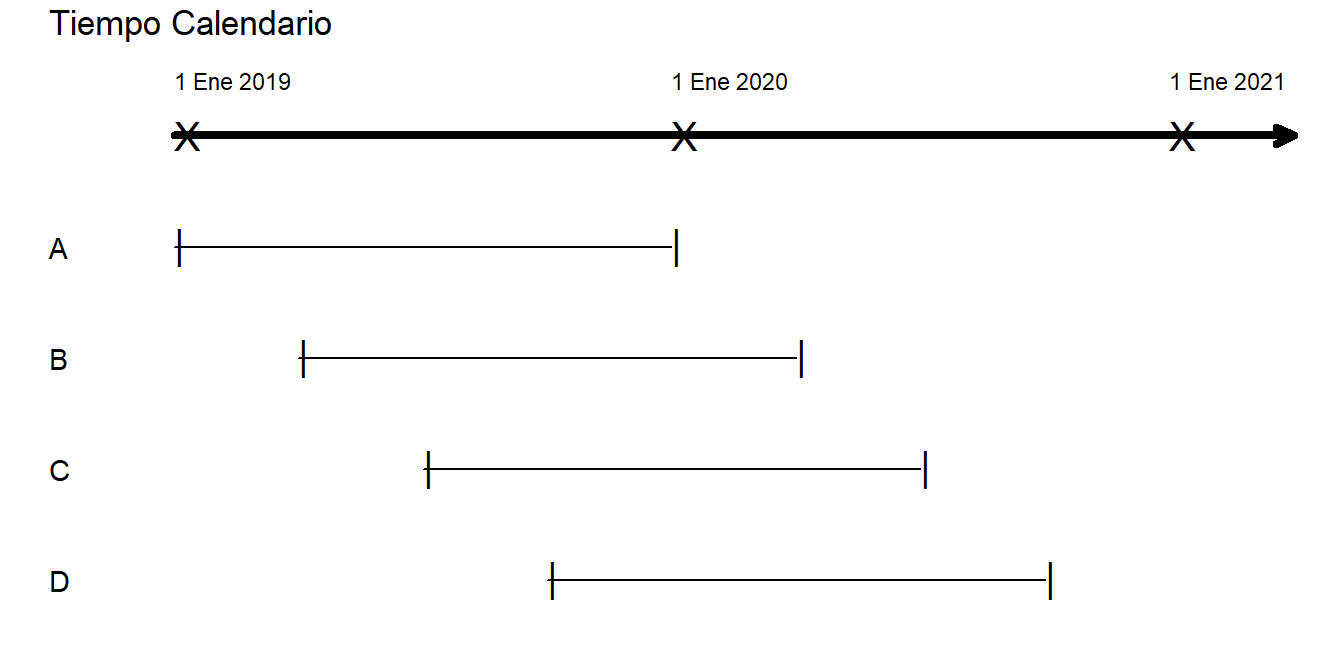
\includegraphics[width=0.5\linewidth]{LossDataAnalytics_files/figure-latex/Exposures-1} 

}

\caption{(ref:Exposures)}\label{fig:Exposures}
\end{figure}

Algunas medidas de exposición utilizadas comúnmente son:

\begin{itemize}
\tightlist
\item
  exposiciones emitidas, la cantidad de exposición en las pólizas emitidas (devengadas y no devengadas) durante el periodo en cuestión,
\item
  exposiciones devengadas, las unidades de exposición efectivamente expuestas a la pérdida durante el periodo, esto es, la cobertura que ya ha sido proporcionada,
\item
  exposiciones no devengadas, representan la porción de las exposiciones emitidas para las que todavía no se ha proporcionado cobertura en este periodo de tiempo, y
\item
  exposiciones en vigor, unidades de exposición expuestas a pérdida en un momento determinado.
\end{itemize}

La \href{Exposiciones\%20para\%20Cuatro\%20Pólizas\%20de\%2012\%20Meses}{Tabla 7.12} muestra cálculos ilustrativos detallados para las cuatro pólizas.

\[
\small{
\begin{matrix}
\begin{array}{cl|cc|cc|cc|c}
  \hline
&  & & & & & &&\text{En Vigor} \\
&\text{Efectivo} & \text{Emitida}& \text{Exposición} & \text{Devengada} &\text{Exposición}& \text{No Devengada} &\text{Exposición}&  \text{Exposición} \\
{Póliza} &\text{Fecha}         & 2019 & 2020 & 2019 & 2020 & 2019 & 2020 & \text{1 Enero 2020} \\   \hline
\text{A}&\text{1 Enero 2019}   & 1,00 & 0,00 & 1,00 & 0,00& 0,00 & 0,00 & 0,00 \\
\text{B}&\text{1 Abril 2019} & 1,00 & 0,00 & 0,75 & 0,25 & 0,25 & 0,00& 1,00 \\
\text{C}&\text{1 Julio 2019}  & 1,00 & 0,00 & 0,50 & 0,50 & 0,50 & 0,00& 1,00 \\
\text{D}&\text{1 Octub 2019}   & 1,00 & 0,00 & 0,25 & 0,75 & 0,75 & 0,00& 1,00 \\ \hline
 &  Total       & 4,00 & 0,00 & 2,50 & 1,50 & 1,50 & 0,00 & 3,00 \\
  \hline
  \hline
\end{array}
\end{matrix}
}
\]
\href{Exposiciones\%20para\%20Cuatro\%20Pólizas\%20de\%2012\%20Meses}{Tabla 7.12}: Exposiciones para Cuatro Pólizas de 12 Meses

Esta medida de resumen se suele denominar método del año de calendario, en contraste al denominado método del año de póliza. En el último método, todas las pólizas empiezan a principios de año. Este método es útil para los métodos de tarificación basados en contratos individuales que nosotros no trataremos aquí.

Del mismo modo que para las exposiciones, podemos resumir (o agregar) primas. Las primas, igualmente, pueden ser también \emph{emitidas}, \emph{devengadas}, \emph{no devengadas}, o \emph{en vigor}. Considerar el ejemplo siguiente.

\textbf{Ejemplo. 7.5.1. CAS Examen 5, 2003, Número 10.} Una póliza de 12 meses ha sido emitida el 1 de marzo de 2002 con una prima de 900\$. El 31 de diciembre de 2002, ¿cuál de los siguientes casos es cierto?

\[
\small{
\begin{matrix}
\begin{array}{l|ccc}
  \hline
& \text{Año Calendario} & \text{Año Calendario} \\
& \text{2002 Emitida} & \text{2002 Devengada} & \text{En vigor} \\
& \text{Prima} & \text{Prima}  & \text{Prima}  \\\hline
A. & 900 & 900 & 900 \\
B. & 750 & 750 & 900 \\
C. & 900 & 750 & 750 \\
D. & 750 & 750 & 750 \\
E. & 900 & 750 & 900 \\\hline
\end{array}
\end{matrix}
}
\]

Únicamente la prima devengada difiere de la prima emitida y la prima en vigor y, por tanto, es necesario calcularla. Así, la prima devengada a 31 de diciembre es igual a \(900\$ \times 10/12 = 750\$\). Respuesta E.

\begin{center}\rule{0.5\linewidth}{0.5pt}\end{center}

\hypertarget{siniestros-reclamaciones-y-pagos}{%
\subsection{Siniestros, Reclamaciones y Pagos}\label{siniestros-reclamaciones-y-pagos}}

En términos generales, los términos siniestro y reclamación se refieren a la cantidad de la compensación pagada o potencialmente pagable al reclamante bajo los términos previstos en la póliza de seguro. Las definiciones pueden variar:

\begin{itemize}
\tightlist
\item
  A veces, el término \emph{reclamación} se utiliza indistintamente con el término \emph{siniestro}.
\item
  En algún seguro y en fuentes actuariales, el término \emph{siniestro} es utilizado como la cantidad del daño ocasionado en un evento asegurado. La \emph{reclamación} es la cantidad pagada por el asegurador, con alguna diferencia debido a las franquicias, límites de la póliza, y similares.
\item
  En usos económicos, una \emph{reclamación} es una demanda de pago hecha por un asegurado o por una víctima que actúa como tercero bajo los términos y condiciones de un contrato de seguro y el \emph{siniestro} es la cantidad pagada por el asegurador.
\end{itemize}

En este texto seguiremos el segundo punto. Con todo, al leer otras referencias, deberemos estar alerta sobre las definiciones utilizadas para los términos siniestro y reclamación.

Para establecer más terminología, es útil seguir el cronograma de una reclamación tal y como se desarrolla. En la Figura \ref{fig:ClaimDevelopment}, el evento de la reclamación ocurre en el momento \(t_1\) y se notifica a la compañía aseguradora en el momento \(t_3\). Puede haber un largo intervalo de tiempo entre la ocurrencia y la notificación, tal que dicho intervalo de tiempo incluya el momento de cierre del periodo de reporte financiero (\(t_2\)), conocido como fecha de evaluación. En este caso, la reclamación se denomina como pendiente de declaración en esta fecha de evaluación.

Después de ser notificada, puede haber uno o más pagos de siniestro. No siempre todos los pagos pueden ser realizados antes de la próxima fecha de evaluación (\(t_4\)).

A medida que la reclamación se desarrolla, finalmente, la compañía considera sus obligaciones financieras para que la reclamación sea resuelta y declara la reclamación como cerrada. Aun así, es posible que nuevos hechos ocurran y que la reclamación deba ser reabierta, dando lugar a pagos de siniestro adicionales antes de ser cerrada otra vez.



\begin{figure}

{\centering 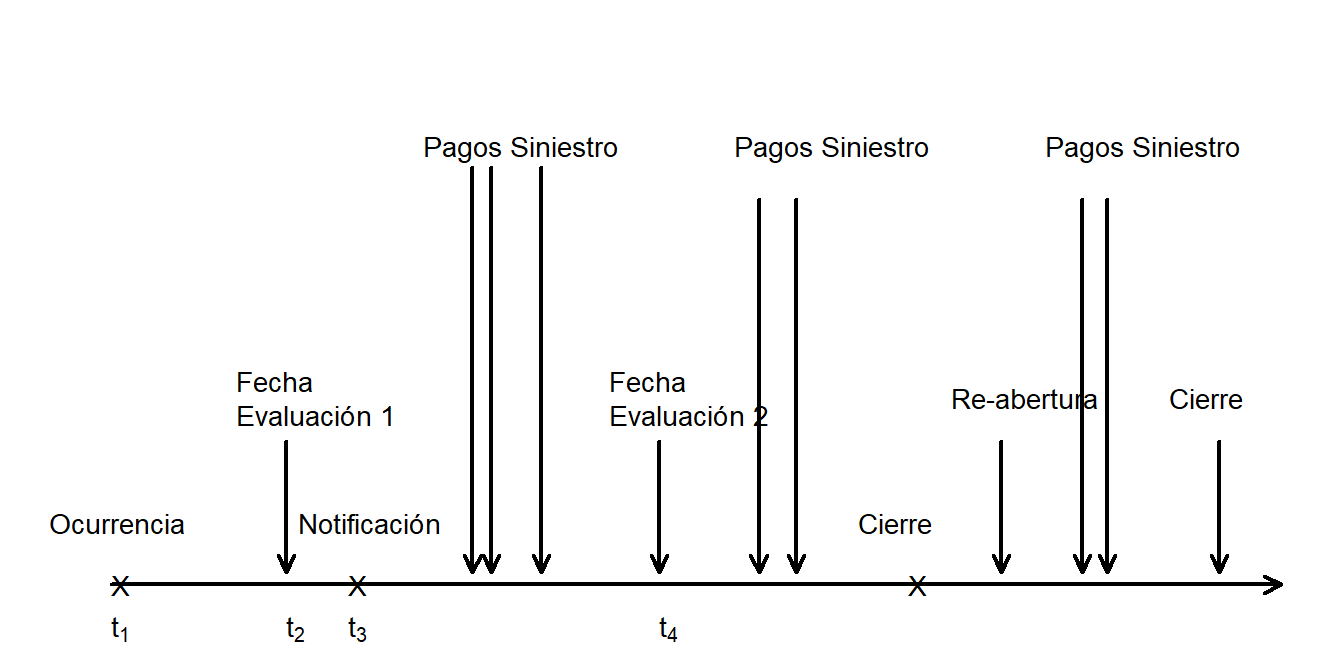
\includegraphics[width=0.75\linewidth]{LossDataAnalytics_files/figure-latex/ClaimDevelopment-1} 

}

\caption{Cronograma del Desarrollo de una Reclamación.}\label{fig:ClaimDevelopment}
\end{figure}

\begin{itemize}
\tightlist
\item
  Fecha de Accidente - la fecha de ocurrencia que dio origen a la reclamación. También conocida como \emph{fecha de siniestro} o \emph{fecha de ocurrencia}.
\item
  Fecha de Declaración - la fecha en la que el asegurador recibe la notificación de la reclamación. Los siniestros (o reclamaciones) no conocidos actualmente por el asegurador se conocen como siniestros pendientes de declaración o \emph{incurred but not reported (IBNR) claims}, en inglés.
\end{itemize}

Hasta que la reclamación está resuelta o liquidada, la reclamación declarada se considera como una reclamación abierta. Una vez la reclamación está resuelta, se clasifica como \emph{reclamación cerrada}. En algunos casos, puede ocurrir algo más después que la reclamación esté cerrada, y la reclamación puede ser reabierta.

Recordemos que un siniestro es la cantidad pagada o pagable a un reclamante bajo los términos previstos en una póliza de seguro. Además, tenemos

\begin{itemize}
\tightlist
\item
  \emph{Siniestros pagados} son aquellos siniestros de un periodo determinado que ya han sido pagados a los reclamantes.
\item
  Cuando hay una previsión de que un pago deberá ser hecho en el futuro, la reclamación tendrá una reserva por siniestros pendientes de liquidación y pago, \emph{case reserve} en inglés, que representa la cantidad estimada de ese pago.
\item
  \emph{Siniestros declarados}, también conocidos en inglés por \emph{case incurred}, son Siniestros pagados + Reserva de siniestros pendientes de liquidación y pago.
\end{itemize}

La \emph{siniestralidad definitiva} es la cantidad de dinero necesaria para cerrar y resolver todas las reclamaciones para un grupo determinado de pólizas.

\hypertarget{S:CompareMethods}{%
\subsection{Comparación de los Métodos de Prima Pura y Ratio de Siniestralidad}\label{S:CompareMethods}}

Una vez que hemos aprendido como las exposiciones, las primas, y las reclamaciones se desarrollan en el tiempo, podemos considerar cómo pueden ser utilizadas para la tarificación. Hemos visto que los aseguradores ofrecen muchos tipos diferentes de pólizas que dan cobertura a diferentes asegurados con diferentes cantidades de riesgos. Esta agregación se denomina a veces como mezcla de negocio. Es importante hacer notar que a lo largo del tiempo pueden existir cambios en esta mezcla ya que los asegurados van y vienen, las cantidades de los riesgos varían, etcétera. Las exposiciones, las primas, y los tipos de riesgos de un informe financiero previo pueden no ser representativos del periodo para el que se calculen las tarifas. El proceso de extrapolar exposiciones, primas, y tipos de riesgo es conocido como \textbf{de tendencia}. Por ejemplo, una prima devengada nivelada es aquella prima devengada que resultaría de considerar para todo el periodo las tarifas aplicadas según el periodo efectivo de experiencia. La mayoría de métodos de tendencia son matemáticamente sencillos en la práctica, aunque pueden complicarse por circunstancias contractuales y administrativas. Para más detalle, dirigimos al lector a las referencias estándares tales como \citet{werner2016basic} y \citet{friedland2013fundamentals}.

\hypertarget{muxe9todo-de-ratio-de-siniestralidad}{%
\subsubsection*{Método de Ratio de Siniestralidad}\label{muxe9todo-de-ratio-de-siniestralidad}}
\addcontentsline{toc}{subsubsection}{Método de Ratio de Siniestralidad}

La expresión para el factor de cambio de tarifa del método de ratio de siniestralidad en la ecuación \eqref{eq:IndicatedChangeFactor} supone una determinada consistencia en la experiencia de la cartera a lo largo del tiempo. Para otro enfoque, podemos definir la ratio de siniestralidad histórica como:

\[
\small{
RS_{histórica} = \frac{\text{siniestros históricos}}{\text{exposición devengada del periodo histórico }\times \text{tarifa actual}}.
}
\]

Aquí, podemos pensar en la exposición devengada del periodo histórico \(\times\) tarifa actual como la prima histórica.

Utilizando la ecuación \eqref{eq:PremiumEquation}, podemos escribir una ratio de siniestralidad como
\[
\small{
RS = \frac{\text{Siniestros}}{\text{Primas}}=\frac{1-V-Q}{\text{(Siniestros + Fijos)}/\text{Siniestros}}=\frac{1-V-Q}{1+G} ~,
}
\]

donde \(G = \text{Fijos} / \text{Siniestros}\), es la ratio de gastos fijos sobre siniestros. Con esta expresión, definimos la \emph{ratio de siniestralidad objetivo}

\[
\small{
RS_{objetivo} =
\frac{1-V-Q}{1+G} = \frac{1-\text{factor de gastos variables – factor de beneficio y contingencias}}
{1+\text{ratio de gastos fijos sobre siniestros}}  .
}
\]

Con esto, el factor de cambio de tarifa es

\begin{equation}
\small{
FC =\frac{RS_{histórica}}{RS_{objetivo}}.
}
\label{eq:RevisedIndicatedChangeFactor}
\end{equation}

Comparando la ecuación \eqref{eq:IndicatedChangeFactor} con \eqref{eq:RevisedIndicatedChangeFactor}, podemos ver que la última ofrece más flexibilidad para incorporar explícitamente tendencias históricas. Como el método de ratio de siniestralidad está basado en cambios de proporciones, esta flexibilidad está ciertamente garantizada.

\hypertarget{comparaciuxf3n-de-muxe9todos}{%
\subsubsection*{Comparación de Métodos}\label{comparaciuxf3n-de-muxe9todos}}
\addcontentsline{toc}{subsubsection}{Comparación de Métodos}

Suponiendo que exposiciones, primas y reclamaciones han sido tratadas para ser representativas del periodo para el que las tarifas están siendo calculadas, estamos preparados para comparar los métodos de tarificación de prima pura y ratio de siniestralidad. Empezaremos haciendo notar que con los mismos datos de entrada, estas dos aproximaciones producen los mismos resultados. Esto es, son algebraicamente equivalentes. Sin embargo, se basan en diferentes enfoques:

\[
\small{
\begin{array}{l|l}\hline
\text{Método Prima Pura} & \text{Método Ratio Siniestralidad} \\ \hline
\text{Basado en exposiciones} & \text{Basado en primas} \\
\text{No requiere tarifas existentes} & \text{Requiere tarifas existentes} \\
\text{No utiliza primas niveladas} & \text{Utiliza primas niveladas} \\
\text{Produce tarifas} & \text{Produce cambios de tarifas} \\
  \hline
\end{array}
}
\]

Comparando los métodos de tarificación de prima pura y ratio de siniestralidad, podemos ver que:

\begin{itemize}
\tightlist
\item
  El método de prima pura requiere una exposiciones bien definidas y sensibles al cambio.
\item
  El método de ratio de siniestralidad no puede ser utilizado para un nuevo ramo porque produce cambios de la tarifa actual.
\item
  El método de prima pura es preferible cuando puede ser difícil calcular la prima nivelada. En algunos casos, como los ramos de negocios donde los ajustes de la tarifa del riesgo individual se hacen a pólizas individuales, es difícil determinar la prima devengada nivelada necesaria para utilizar el método de ratio de siniestralidad.
\end{itemize}

En muchos países desarrollados como los EE.UU. donde la mayoría de ramos existen desde hace décadas, el método de ratio de siniestralidad es el más popular.

\textbf{Ejemplo. 7.5.2. CAS Examen 5, 2006, Número 36.} Sea la información siguiente :

\begin{itemize}
\tightlist
\item
  Primas devengadas niveladas para el periodo de experiencia = 500.000\$
\item
  Siniestros con tendencia según periodo de experiencia = 300.000\$
\item
  Exposición devengada del periodo de experiencia = 10.000
\item
  Factor de gastos variables = 23\%
\item
  Gastos fijos = 21.000\$
\item
  Factor de beneficios y contingencias = 5\%
\end{itemize}

\begin{enumerate}
\def\labelenumi{(\alph{enumi})}
\item
  Calcula el cambio de nivel de tarifa utilizando el método de ratio de siniestralidad.
\item
  Calcula el cambio de nivel de tarifa utilizando el método de prima pura.
\item
  Describe una situación en la que es preferible utilizar el método de ratio de siniestralidad, y una situación en la que es preferible utilizar el método de prima pura.
\item
  calcularemos las ratios de siniestralidad histórica y objetivo, y entonces haremos el cociente de las dos para obtener el cambio de tarifa. La ratio de siniestralidad histórica es
  \[
  \small{
  RS_{histórica} =  \frac{\text{siniestros históricos }}{\text{primas históricas}} =\frac{300000}{500000} = 0,60.
  }
  \]
\end{enumerate}

La ratio de siniestralidad objetivo es:

\[
\small{
\begin{matrix}
\begin{array}{ll}
RS_{objetivo}
&= \frac{1-V-Q}{1+G} = \frac{1-\text{factor gastos variables – factor beneficios y contingencias}}
{1+\text{ratio de gastos fijos sobre siniestros}}\\
&= \frac{1-0,23 – 0,05}{1+0,07} = 0,673  .
\end{array}
\end{matrix}
}
\]

Donde la ratio de gastos fijos sobre siniestros es \(G = \frac{21000}{300000} = 0,07\).

Por tanto, el (nuevo) cambio de nivel de tarifa es

\[
\small{
FC =\frac{RS_{histórica}}{RS_{objetivo}} -1  = \frac{0,60}{0,673} -1 = -10,8\%.
}
\]
(b) Utilizando el método de prima pura, el factor de cambio \(FC\) es

\[
\small{
\begin{matrix}
\begin{array}{ll}
FC
&= \frac{\text{Siniestros + Fijos}}{\text{Prima} \times (1 - Q - V)}\\
&= \frac{300000+ 21000}{500000 \times (1 – 0,23 – 0,05)} = 0,892.
\end{array}
\end{matrix}
}
\]

Por tanto, el factor de cambio de nivel de tarifa es \(0,892 -1 = -10,8\%\).

\begin{enumerate}
\def\labelenumi{(\alph{enumi})}
\setcounter{enumi}{2}
\tightlist
\item
  El método de ratio de siniestralidad es preferible cuando la unidad de exposición no está disponible.
\end{enumerate}

El método de ratio de siniestralidad es preferible cuando la unidad de exposición no es razonablemente compatible entre riesgos.

El método de prima pura es preferible para un nuevo ramo.

El método de prima pura es preferible cuando las primas niveladas son difíciles de calcular.

\hypertarget{S:GiniStatistic}{%
\section{Selección de Prima}\label{S:GiniStatistic}}

\begin{center}\rule{0.5\linewidth}{0.5pt}\end{center}

En esta sección, se aprende cómo:

\begin{itemize}
\tightlist
\item
  Describir distribuciones no simétricas mediante una curva de Lorenz y un índice de Gini
\item
  Definir una curva de rendimiento y el correspondiente estadístico de Gini
\item
  Utilizar la curva de rendimiento y el estadístico de Gini para seleccionar la prima mediante validación cruzada
\end{itemize}

\begin{center}\rule{0.5\linewidth}{0.5pt}\end{center}

En una cartera de contratos de seguro, los aseguradores reciben primas y pagan siniestros. Después de realizar sendos ajustes para los gastos y las consideraciones sobre beneficio, podrían resultar útiles herramientas para comparar las distribuciones de primas y siniestros a la hora de seleccionar un principio de cálculo de la prima.

\hypertarget{curva-de-lorenz-cluxe1sica}{%
\subsection{Curva de Lorenz Clásica}\label{curva-de-lorenz-cluxe1sica}}

En economía del bienestar, es común comparar distribuciones vía la curva de Lorenz, desarrollada por Max Otto Lorenz \citep{lorenz1905methods}. Una curva de Lorenz es un gráfico de la proporción de una población en el eje horizontal y una función de distribución de interés en el eje vertical. Normalmente se utiliza para representar distribuciones de ingresos. Cuando la distribución de ingresos está perfectamente alineada con la distribución de población, la curva de Lorenz resultante es una recta de 45 grados denominada como línea de igualdad. Como el gráfico compara dos funciones de distribución, podemos pensar en la curva de Lorenz como un tipo de pp plot que fue introducido en la Sección \ref{S:MS:GraphComparison}. El área entre la curva de Lorenz y la línea de igualdad es una medida de la discrepancia entre las distribuciones de ingresos y población. Dos veces esta área nos proporciona el conocido índice de Gini, introducido por Corrado Gini en 1912.

\textbf{Ejemplo -- Curva de Lorenz Clásica.} Para un ejemplo asegurador, la Figura \ref{fig:ClassicLorenz} muestra una distribución de los siniestros de un seguro. Esta figura está basada en una muestra aleatoria de 2000 siniestros. El lado izquierdo muestra un histograma con asimetría por la derecha de los siniestros. El lado derecho proporciona la correspondiente curva de Lorenz, mostrando de nuevo una distribución asimétrica. Por ejemplo, la flecha marca el punto donde el 60 por ciento de los asegurados tienen el 30 por ciento de los siniestros. La línea de 45 grados es la línea de igualdad; si cada asegurado tuviera la misma siniestralidad, entonces la distribución de siniestralidad coincidiría con esta línea. El índice de Gini, dos veces la área entre la curva de Lorenz y la línea de 45 grados, es un 37.6 por ciento para este conjunto de datos.

\begin{figure}

{\centering 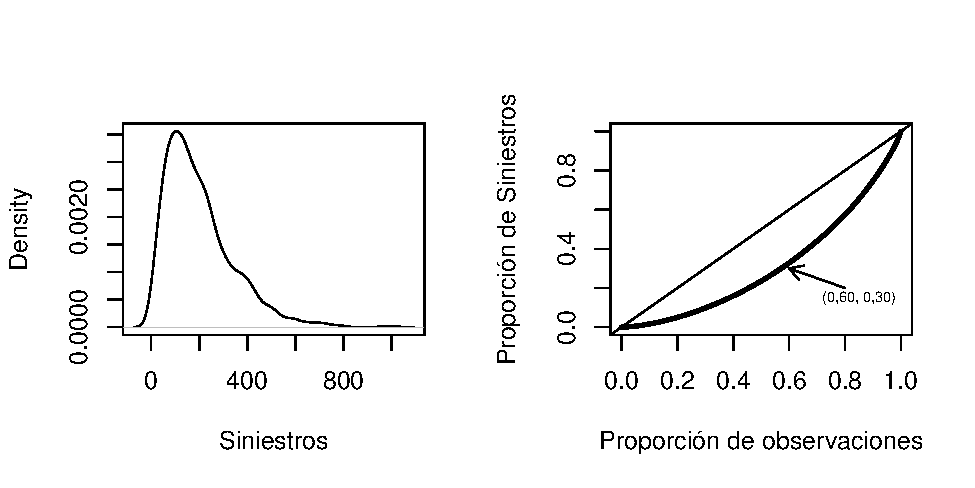
\includegraphics[width=0.9\linewidth]{LossDataAnalytics_files/figure-latex/ClassicLorenz-1} 

}

\caption{Distribución de los Siniestros de un Seguro. El lado izquierdo es la función de densidad de los siniestros. El lado derecho muestra los mismos datos mediante la curva de Lorenz.}\label{fig:ClassicLorenz}
\end{figure}

\hypertarget{curva-de-rendimiento-y-estaduxedstico-de-gini}{%
\subsection{Curva de Rendimiento y Estadístico de Gini}\label{curva-de-rendimiento-y-estaduxedstico-de-gini}}

Ahora podemos introducir una modificación de la clásica curva de Lorenz y del índice de Gini que sea útil para aplicaciones del seguro. Específicamente, introducimos una curva de rendimiento que, en este caso, es un gráfico de la distribución de siniestros versus la de primas, donde ambas están ordenadas por prima. Para concretar ideas, proporcionamos alguna notación y consideramos \(i=1, \ldots, n\) pólizas. Para la \(i\)-ésima póliza,

\begin{itemize}
\tightlist
\item
  \(y_i\) denota el siniestro del seguro,
\item
  \(\mathbf{x}_i\) es un conjunto de variables de tarificación conocidas por el analista, y
  \(P_i=P(\mathbf{x}_i)\) es la prima asociada, que es una función que depende de \(\mathbf{x}_i\).
\end{itemize}

El conjunto de información utilizada para calcular la curva de rendimiento para la \(i\)-ésima póliza es \((y_i, P_i)\).

\hypertarget{curva-de-rendimiento}{%
\subsubsection*{Curva de rendimiento}\label{curva-de-rendimiento}}
\addcontentsline{toc}{subsubsection}{Curva de rendimiento}

En primer lugar, es conveniente ordenar el conjunto de pólizas según las primas (de más pequeñas a más grandes) y, a continuación, calcular las distribuciones de primas y siniestros. La distribución de primas es
\begin{equation}
\hat{F}_P(s) =  \frac{ \sum_{i=1}^n P_i ~\mathrm{I}(P_i \leq s) }{\sum_{i=1}^n P_i}   ,
\label{eq:EmpPremDF}
\end{equation}

Y la distribución de siniestros es

\begin{equation}
\hat{F}_{L}(s) =  \frac{ \sum_{i=1}^n y_i ~\mathrm{I}(P_i \leq s) }{\sum_{i=1}^n y_i} ,
\label{eq:EmpLossDF}
\end{equation}

donde \(\mathrm{I}(\cdot)\) es una función indicador, que devuelve 1 si el acontecimiento es cierto y cero en caso contrario. Para un valor dado \(s\), \(\hat{F}_P(s)\) nos da la proporción de primas menores o iguales a \(s\), y \(\hat{F}_{L}(s)\) nos da la proporción de siniestros para aquellos asegurados con primas menores o iguales a \(s\). El gráfico \(\left(\hat{F}_P(s),\hat{F}_{L}(s) \right)\) es conocido como *curva de rendimiento**.

\textbf{Ejemplo -- Distribución de Siniestralidad.} Suponemos que tenemos \(n=5\) asegurados con el siguiente historial. Los datos han sido ordenados por primas.

\begin{longtable}[]{@{}lcllrrr@{}}
\toprule
Variable & \(i\) & 1 & 2 & 3 & 4 & 5 \\
\midrule
\endhead
Prima & \(P(\mathbf{x}_i)\) & 2 & 4 & 5 & 7 & 16 \\
Primas Acumuladas & \(\sum_{j=1}^i P(\mathbf{x}_j)\) & 2 & 6 & 11 & 18 & 34 \\
Siniestralidad & \(y_i\) & 2 & 5 & 6 & 6 & 17 \\
Siniest. Acumul. & \(\sum_{j=1}^i y_j\) & 2 & 7 & 13 & 19 & 36 \\
\bottomrule
\end{longtable}

La Figura \ref{fig:LorenzVsOrdered} compara la curva de Lorenz con la curva de rendimiento. En el lado izquierdo se muestra la curva de Lorenz. En el eje horizontal tenemos las proporciones acumuladas de asegurados (0, 0,2, 0,4, y en adelante) y en el eje vertical tenemos la proporción acumulada de siniestros (0, 2/36, 7/36, y en adelante). Para la curva de Lorenz, primero ordenamos por la cuantía del siniestro (lo que para este sencillo ejemplo representa lo mismo que ordenar por primas). Esta figura muestra una gran separación entre las distribuciones de siniestralidad y asegurados.

El lado derecho nos muestra la curva de rendimiento. Como las observaciones están ordenadas por prima, el primer punto después del origen (leyendo de izquierda a derecha) es (2/34, 2/36). El segundo punto es (6/34, 7/36). De la figura, vemos que hay poca separación entre siniestros y primas.

\begin{figure}

{\centering 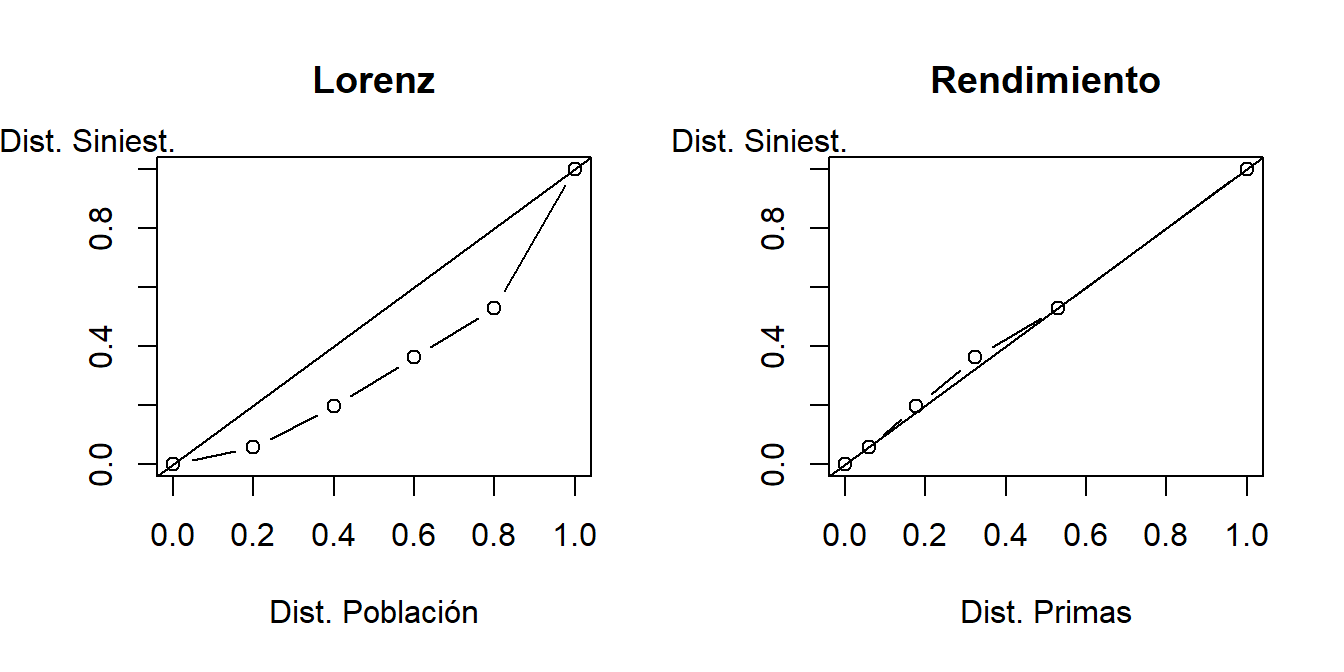
\includegraphics[width=0.9\linewidth]{LossDataAnalytics_files/figure-latex/LorenzVsOrdered-1} 

}

\caption{Curva Lorenz versus Curva Rendimiento}\label{fig:LorenzVsOrdered}
\end{figure}

\begin{center}\rule{0.5\linewidth}{0.5pt}\end{center}

La curva de rendimiento puede ser útil al analista que trata de formar carteras rentables para el asegurador. Por ejemplo, supongamos que \(s\) es escogido para representar el percentil 95 de la distribución de primas. Entonces, el eje horizontal, \(\hat{F}_P(s)\), representa la fracción de primas para esta cartera y el eje vertical, \(\hat{F}_L(s)\), la fracción de siniestros para esta cartera. Cuando se plantean los principios de tarificación, los analistas buscan evitar situaciones no rentables y conseguir beneficios.

La esperanza del numerador en la ecuación \eqref{eq:EmpLossDF} es \(\sum_{i=1}^n \mathrm{E}~ y_i=\sum_{i=1}^n \mu_i\). Así, si el principio de tarificación es escogido tal que \(P_i= \mu_i\), entonces esperaremos una relación muy próxima entre las distribuciones de prima y siniestralidad, resultando una línea de 45 grados. La línea de 45 grados iguala primas y siniestros, una situación de equilibrio que es una referencia para la tarificación de seguros.

\hypertarget{estaduxedstico-de-gini}{%
\subsubsection*{Estadístico de Gini}\label{estaduxedstico-de-gini}}
\addcontentsline{toc}{subsubsection}{Estadístico de Gini}

La curva de Lorenz clásica muestra la proporción de asegurados en el eje horizontal y la función de distribución de la siniestralidad en el eje vertical. La curva de rendimiento extiende la curva de Lorenz clásica en dos maneras, (1) a través de la ordenación de riesgos y precios por primas y (2) permitiendo que los precios varíen por observación. Podemos resumir la curva de rendimiento de la misma manera que la curva de Lorenz clásica, utilizando un estadístico de Gini, definido como dos veces el área entre la curva y la línea de 45 grados. El analista busca las curvas de rendimiento que mejor se aproximen a la línea de 45 grados; éstas tienen menos separación entre las distribuciones de siniestros y primas y, por tanto, un estadístico de Gini menor.

Específicamente, el estadístico de Gini puede ser calculado como sigue. Suponemos que la curva de rendimiento empírica viene dada por \(\{ (a_0=0, b_0=0), (a_1, b_1), \ldots,\) \((a_n=1, b_n=1) \}\) para una muestra de \(n\) observaciones. Aquí, utilizamos \(a_j = \hat{F}_P(P_j)\) y \(b_j = \hat{F}_{L}(P_j)\). Entonces, el estadístico de Gini empírico es

\begin{eqnarray}
\widehat{Gini} 
&=&  2\sum_{j=0}^{n-1} (a_{j+1} - a_j) \left \{
\frac{a_{j+1}+a_j}{2} - \frac{b_{j+1}+b_j}{2} \right\} \nonumber \\
&=& 1 - \sum_{j=0}^{n-1} (a_{j+1} - a_j) (b_{j+1}+b_j) .
\label{eq:GiniDefn}
\end{eqnarray}

Para comprender la fórmula del estadístico de Gini, aquí presentamos un croquis de un paralelogramo que conecta los puntos \((a_1, b_1)\), \((a_2, b_2)\), y una línea de 45 grados. Podemos utilizar geometría básica para comprobar que el área de la figura es \(Área = (a_2 - a_1) \left \{\frac{a_2+a_1}{2} - \frac{b_2+b_1}{2} \right\}\). La definición del estadístico de Gini en la ecuación \eqref{eq:GiniDefn} es sencillamente dos veces la suma del paralelogramo. La segunda igualdad en la ecuación \eqref{eq:GiniDefn} es el resultado de aplicar sencillos cálculos.

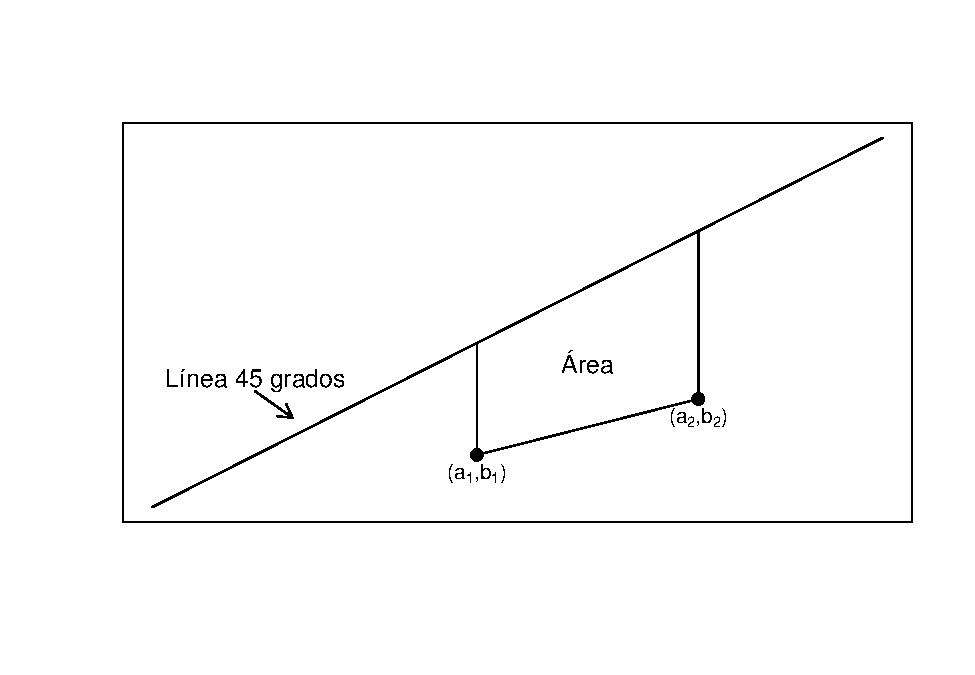
\includegraphics{LossDataAnalytics_files/figure-latex/unnamed-chunk-176-1.pdf}

\begin{center}\rule{0.5\linewidth}{0.5pt}\end{center}

\textbf{Ejemplo -- Distribución de Siniestralidad: Continuación.} El estadístico de Gini para la curva de Lorenz (lado izquierdo de la Figura \ref{fig:LorenzVsOrdered}) es un 34.4 por ciento. En contraste, el estadístico de Gini para la curva de rendimiento (lado derecho) es un 1.7 por ciento.

\hypertarget{validaciuxf3n-cruzada}{%
\subsection{Validación Cruzada}\label{validaciuxf3n-cruzada}}

Los beneficios de la validación cruzada (out-of-sample validation, en inglés) para la selección de modelos fueron introducidos en la Sección 4.2. Ahora mostraremos el uso del estadístico de Gini y la curva de rendimiento en este contexto. El procedimiento sería:

\begin{enumerate}
\def\labelenumi{\arabic{enumi}.}
\tightlist
\item
  Usar la muestra de entrenamiento para la estimación de los diferentes modelos a comparar, cada uno produciendo una función de prima.
\item
  Designar una muestra de validación a partir de \(\{(y_i, \mathbf{x}_i), i=1,\ldots,n\}\).
\item
  Utilizar las variables explicativas de la muestra de validación para calcular las primas de la forma \(P(\mathbf{x}_i)\).
\item
  Calcular el estadístico de Gini para cada modelo. Escoger el modelo con el menor estadístico de Gini.
\end{enumerate}

*Ejemplo -- Tarificación Comunitaria versus Primas que Varían por Estado.** Suponemos que tenemos experiencia histórica de 25 estados y que, para cada estado, tenemos disponibles 200 observaciones que pueden servir para pronosticar siniestros futuros. Por simplicidad, suponemos que el analista conoce que estos siniestros siguen, o fueron generados por, una distribución gamma con un parámetro de forma común igual a 5. Desconocido para el analista, los parámetros de escala varían para cada estado, desde 20 a 66.

\begin{itemize}
\tightlist
\item
  Para calcular las primas de base, el analista supone un parámetro de escala que es común para todos los estados y que se estima a partir de los datos. Podemos pensar de esta prima común como una prima basada en un principio de tarificación comunitaria.
\item
  Como alternativa, el analista deja que los parámetros de escala varíen para cada estado y otra vez utilizará los datos para estimar dichos parámetros.
\end{itemize}

Una muestra de validación de 100 siniestros está disponible para cada estado. Para cada uno de los dos procedimientos de tarificación, determinar la curva de rendimiento y el correspondiente estadístico de Gini. Escoger el procedimiento de tarificación con el menor estadístico de Gini.

\begin{center}\rule{0.5\linewidth}{0.5pt}\end{center}

Recordemos que para la distribución gamma la media es igual al producto de los parámetros de forma y escala, para nuestro ejemplo, 5 veces el parámetro de escala. Podemos comprobar que los estimadores máximo-verosímiles son sencillamente las medias históricas.

Para nuestra prima base, suponemos una distribución común para todos los estados. Para estos datos simulados, la media de los siniestros en la muestra de entrenamiento es \(P_1\)=221.36.

Como alternativa, utilizamos las medias para cada estado en concreto; estas medias forman nuestras primas \(P_2\). Como este ejemplo utiliza medias que varían para cada estado, esperaremos que este procedimiento alternativo sea preferido al procedimiento de tarificación comunitaria.

Los siniestros de la muestra de validación fueron generados a partir de la misma distribución gamma de la muestra de entrenamiento, con 100 observaciones para cada estado. El siguiente código en \texttt{R} nos muestra cómo calcular las curvas de rendimiento.

\begin{figure}

{\centering 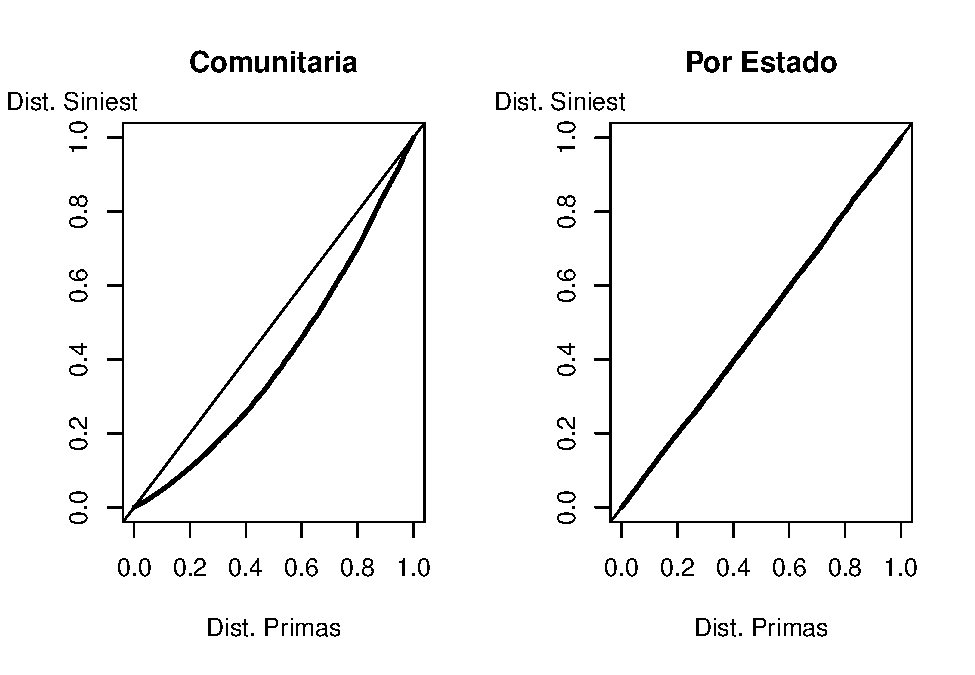
\includegraphics[width=0.9\linewidth]{LossDataAnalytics_files/figure-latex/unnamed-chunk-179-1} 

}

\end{figure}

Para estos datos, los estadísticos de Gini son un 19.6 por ciento para la prima de tarificación comunitaria o plana y un -0.702 por ciento para la prima alternativa que discrimina por estado. Esto indica que el procedimiento alternativo es mucho más preferible que el procedimiento de tarificación comunitaria.

\begin{center}\rule{0.5\linewidth}{0.5pt}\end{center}

\hypertarget{discusiuxf3n}{%
\subsubsection*{Discusión}\label{discusiuxf3n}}
\addcontentsline{toc}{subsubsection}{Discusión}

En la modelización de los siniestros de seguros, las medidas estándar de validación cruzada no son las más informativas debido a las altas proporciones de ceros (pólizas con ninguna reclamación) y a la alta asimetría de la distribución para los valores positivos. En contraste, el estadístico de Gini funciona muy bien en presencia de muchos ceros (véase la demostración en \citep{frees2014insurance}).

El valor de las curvas de rendimiento y los estadísticos de Gini han sido recientemente tratadas en el artículo de \citet{denuit2019concentrationGini}. Las propiedades de una versión extendida, tratando con relatividades para las primas nuevas, fue desarrollada por \citet{frees2011summarizing} y \citet{frees2014insurance}. En estos artículos se pueden encontrar las fórmulas para los errores estándares y otra información adicional.

\hypertarget{otros-recursos-y-colaboradores}{%
\section{Otros Recursos y Colaboradores}\label{otros-recursos-y-colaboradores}}

Este capítulo sirve como puente entre la introducción técnica de este libro y una introducción a la tarificación llevada a cabo por los actuarios en la práctica. Para los lectores interesados en aprender aspectos prácticos de la tarificación, recomendamos las introducciones de la Society of Actuaries en \citet{friedland2013fundamentals} y por la Casualty Actuarial Society en \citet{werner2016basic}. Para una introducción clásica de la gestión del riesgo para la tarificación, véase \citet{niehaus2003risk}. Véase también \citet{finger2006risk} y \citet{frees2014frequency}.

\citet{buhlmann1985premium} fue el primero en la literatura académica en argumentar que la tarificación debería ser hecha primero a nivel de la cartera (se refería a esto como aproximación \emph{top down}) para, posteriormente, ser ajustada a nivel de los contratos individuales. Véase también la discusión en \citet{kaas2008modern}, Capítulo 5.

Para más referencias sobre los principios de tarificación, un tratamiento clásico es \citet{gerber1979introduction} y una aproximación más moderna es \citet{kaas2008modern}. Para una discusión desde un punto de vista económico-financiero, véase \citet{bauer2013financial}.

\begin{itemize}
\tightlist
\item
  \textbf{Edward W. (Jed) Frees}, University of Wisconsin-Madison, y \textbf{José Garrido}, Concordia University son los autores principales de la versión inicial de este capítulo. Email: \href{mailto:jfrees@bus.wisc.edu}{\nolinkurl{jfrees@bus.wisc.edu}} y/o \href{mailto:jose.garrido@concordia.ca}{\nolinkurl{jose.garrido@concordia.ca}} para comentarios del capítulo y sugerencias de mejora.
\item
  Revisores de los capítulos, entre otros: escribir a Jed o José para añadir su nombre aquí.
\item
  Traducción al español: Lluís Bermúdez (Universitat de Barcelona)
\end{itemize}

\hypertarget{ts-7.a.-regulaciuxf3n-de-la-tarificaciuxf3n}{%
\subsection*{TS 7.A. Regulación de la Tarificación}\label{ts-7.a.-regulaciuxf3n-de-la-tarificaciuxf3n}}
\addcontentsline{toc}{subsection}{TS 7.A. Regulación de la Tarificación}

La regulación del seguro es necesaria para asegurar la estabilidad financiera de los aseguradores y para proteger a los consumidores. Los aseguradores reciben unas primas a cambio de las promesas de pagar en caso de ocurrencia del evento asegurado. Como en otras instituciones financieras, como los bancos, hay un fuerte interés público en promover la viabilidad económica futura de los aseguradores.

\hypertarget{conducta-de-mercado}{%
\subsubsection*{Conducta de mercado}\label{conducta-de-mercado}}
\addcontentsline{toc}{subsubsection}{Conducta de mercado}

\textless!--- Uno de los aspectos de regulación es conocido como regulación de la \emph{conducta del mercado} - sistemas de control regulatorios que han sido establecidos como requerimiento a los aseguradores para demostrar que están proporcionando unos servicios justos y fiables, incluyendo la regulación del producto. --\textgreater{}

Para ayudar a proteger a los consumidores, los reguladores imponen unas reglas administrativas sobre el comportamiento de los participantes en el mercado. Estas reglas, conocidas como regulación de conductas de mercado, proporcionan sistemas de control regulatorios que disponen que los aseguradores deben demostrar que están proporcionando servicios justos y fiables, incluyendo la tarificación, de acuerdo con los estatutos y controles de una jurisdicción.

\begin{enumerate}
\def\labelenumi{\arabic{enumi}.}
\tightlist
\item
  La \emph{regulación de producto} sirve para proteger a los consumidores asegurando que las provisiones de las pólizas de seguro son razonables y justas, y que no presentan vacíos importantes en cuanto a la cobertura que podrían ser mal entendidos por los consumidores y dejarles desprotegidos.
\item
  El producto asegurador es el contrato de seguro (póliza) y la cobertura que proporciona. Los contratos de seguro están regulados por las siguientes razones:
\end{enumerate}

\begin{enumerate}
\def\labelenumi{\alph{enumi}.}
\tightlist
\item
  Las pólizas de seguro son documentos legales complejos que a menudo son difíciles de interpretar y entender.
\item
  Los aseguradores definen pólizas y las venden al público en un ``o lo tomas o lo dejas''.
\end{enumerate}

La conducta de mercado incluye reglas para los \emph{mediadores} como agentes (quiénes principalmente venden seguros a particulares) y corredores (quiénes principalmente venden seguros a empresas). La conducta de mercado también incluye \emph{regulación de normas de competencia}, diseñada para asegurar un mercado eficaz y competitivo que ofrezca buenas ofertas a los consumidores.

\hypertarget{regulaciuxf3n-de-tarifa}{%
\subsubsection*{Regulación de Tarifa}\label{regulaciuxf3n-de-tarifa}}
\addcontentsline{toc}{subsubsection}{Regulación de Tarifa}

La \emph{regulación de tarifa} sirve de guía en el desarrollo de las primas y por ello es el aspecto principal de este capítulo. Como otros aspectos del control de conducta de mercado, la intención de estas regulaciones es asegurarse que los aseguradores no se benefician injustamente de los consumidores. La regulación de la tarifa (y de la forma de la póliza) es común en todo el mundo.

El grado de regulación varía según el producto de seguro. La regulación de la tarifa es poco común en los seguros de vida. Además, algunos seguros de no-vida, como los ramos más empresariales y el reaseguro, la tarifa está libre de control. La regulación de tarifa es común en el seguro de automóvil, el seguro de salud, los seguros de accidentes laborables, el seguro de responsabilidad civil médica y el seguro de hogar. Estos son mercados en que el seguro es obligatorio o en el que socialmente es deseable una cobertura universal.

Hay tres principios que guían la regulación de tarifa. Las tarifas tienen que:

\begin{itemize}
\tightlist
\item
  ser adecuadas (para mantener la solvencia de la compañía aseguradora),
\item
  pero no excesivas (no tan alta para producir beneficios desorbitados),
\item
  ni injustamente discriminatoria (las diferencias de precio solo deben reflejar diferencias en gastos y reclamaciones esperadas).
\end{itemize}

Recientemente, en los seguros de hogar y automóvil, los temas entrelazados de disponibilidad y accesibilidad, no incluidos explícitamente en los anteriores principios, han ido tomando más importancia en las decisiones regulatorias.

\hypertarget{las-tarifas-no-son-injustamente-discriminatorias}{%
\subsubsection*{Las Tarifas no son Injustamente Discriminatorias}\label{las-tarifas-no-son-injustamente-discriminatorias}}
\addcontentsline{toc}{subsubsection}{Las Tarifas no son Injustamente Discriminatorias}

Algunas regulaciones gubernamentales del seguro restringen la cantidad, o nivel, de las tarifas o primas. Estas regulaciones tratan de conseguir los dos primeros de los tres principios de la regulación sobre tarificación, esto es, que las tarifas deben ser adecuadas pero no excesivas. Este tipo de regulación será discutida en la sección siguiente sobre tipos de regulación tarifaria.

En el seguro de vida, desde hace mucho tiempo ha sido aceptado que es razonable y justo cobrar primas de tarifa diferentes por edad. Por ejemplo, una prima de un seguro de vida difiere dramáticamente entre una persona de 80 años y otra de 20 años. En contraste, no está aceptado utilizar tarifas que difieran por:

\begin{itemize}
\tightlist
\item
  Etnia/raza,
\item
  Afiliación política, o
\item
  Religión.
\end{itemize}

No importa si estos datos pueden ser usados para establecer una significación estadística entre las categorías de cualquiera de estas tres variables. Lo relevante es la decisión social sobre qué se considera como concepto de ``justicia.''

Diferentes jurisdicciones han tomado diferentes posturas sobre qué constituye una variable de tarificación justa. Por ejemplo, en algunas jurisdicciones, para algunos productos aseguradores, el género ya no es una variable permitida. Por ejemplo, en la Unión Europea está prohibido el uso del género del asegurado para el cálculo de las primas. Como otro ejemplo, en los EE.UU., mucho se ha discutido sobre si permitir el uso del índice de crédito del asegurado en la tarifa de su seguro de automóvil. Los índices de crédito están diseñados para medir el grado de responsabilidad financiera del consumidor. En este sentido, algunos argumentan que estos índices de crédito sirven como aproximación de la etnicidad del asegurado y, por tanto, deberían estar prohibidos.

En una época donde los datos están siendo utilizados de múltiples maneras imaginativas, la discusión sobre qué variable constituye una variable justa queda fuera del alcance de este texto. Aun así, es pertinente remarcar que los actuarios y otros analistas de datos pueden contribuir a las discusiones sociales sobre qué constituye una variable de tarificación ``justa'', concretamente, determinando la magnitud de las diferencias de precio cuando se utilizan las variables bajo discusión.

\textless!---¿Debemos recoger estas variables? --\textgreater{}

\hypertarget{tipos-de-regulaciuxf3n-tarifaria}{%
\subsubsection*{Tipos de Regulación Tarifaria}\label{tipos-de-regulaciuxf3n-tarifaria}}
\addcontentsline{toc}{subsubsection}{Tipos de Regulación Tarifaria}

Hay varios métodos, que varían según el nivel regulatorio, con los que los reguladores pueden restringir las tarifas que ofrecen los aseguradores.

El más restrictivo es un sistema regulador de prescripción gubernamental, donde el regulador gubernamental determina y decreta las tarifas, las clasificaciones, la forma, y otras particularidades a las que todos los aseguradores tienen que adherirse. También de carácter restrictivo es un sistema de aprobación previa. En este caso, el asegurador debe presentar las tarifas, las normas y el resto de información requerida por el regulador. Según la normativa, la documentación presentada se considera efectiva tras la finalización de un periodo de tiempo determinado (si el regulador no realiza una acción concreta sobre la documentación presentada, se considera aprobada automáticamente) o cuando el regulador la aprueba formalmente.

El menos restrictivo es un sistema de no presentación o de \emph{mantenimiento de registro} donde el asegurador no necesita presentar documentación sobre tarifas, normas y otros requerimientos al regulador. El regulador periódicamente puede examinar al asegurador para comprobar que actúa con conformidad a la ley. Otro sistema relativamente flexible es el sistema de presentación única, también conocido como tarificación \emph{competitiva}, donde el asegurador sencillamente debe mantener unos documentos para asegurar su conformidad con la ley.

Entre estos dos extremos encontramos (1) presentación y uso, (2) uso y presentación, (3) aprobación previa modificada, y (4) sistemas flexibles de tarifa.

\begin{enumerate}
\def\labelenumi{\arabic{enumi}.}
\tightlist
\item
  Presentación y Uso: El asegurador debe presentar documentación sobre tarifas, normas y otros requerimientos al regulador. Los términos de la documentación son efectivos inmediatamente o tras finalizar un periodo especificado por el regulador.
\item
  Uso y Presentación: El asegurador debe presentar documentación sobre tarifas, normas y otros requerimientos al regulador dentro de un periodo de tiempo especificado después de su primer uso. Los términos de la documentación son efectivos al ser utilizados.
\item
  Aprobación Previa Modificada: Esto es un híbrido entre los sistemas de ``aprobación previa'' y de ``presentación y uso''. Si la revisión de la tarifa sólo responde a un cambio en la experiencia histórica, aplica el sistema de ``presentación y uso''. Sin embargo, si la revisión de tarifa responde a un cambio en los recargos de gastos o en las clasificaciones de la tarifa, entonces aplica la ``aprobación previa''.
\item
  Tarifa Flexible (o Franja Tarifaria): El asegurador puede aumentar o disminuir la tarifa dentro de una ``franja flexible,'' o rango, sin aprobación del regulador. Generalmente, aquí puede aplicar un sistema de ``presentación y uso'' o bien de ``uso y presentación''.
\end{enumerate}

\begin{center}\rule{0.5\linewidth}{0.5pt}\end{center}

Para una profunda revisión de la regulación aseguradora desde una perspectiva global, véase la página web de la \href{https://www.iaisweb.org/home}{Asociación Internacional de Reguladores de Seguro (IAIS, en sus siglas en inglés)}.

\hypertarget{C:RiskClass}{%
\chapter{Clasificación de Riesgos}\label{C:RiskClass}}

\emph{Resumen del capítulo.} Este capítulo motiva el uso de la clasificación de riesgos en la fijación de precios de seguros y presenta a los lectores la regresión de Poisson como un ejemplo destacado de clasificación de riesgos. En la Sección \ref{S:RC:Introduction} explicamos por qué las aseguradoras necesitan incorporar diversas características de riesgo, o factores de tarificación, de los asegurados individuales en los precios de los contratos de seguro. Luego presentamos la Sección \ref{S:RC:PoissonRegression} donde mostramos la regresión de Poisson como una herramienta de fijación de precios para lograr diferencias en las primas. El concepto de exposición también se introduce en esta sección. Como la mayoría de los factores de tarificación son categóricos, en la Sección \ref{S:CatVarMultiTarriff} mostramos cómo se puede incorporar el modelo de tarifa multiplicativa en el modelo de regresión de Poisson en la práctica, junto con ejemplos numéricos para ilustrarlo.

\hypertarget{S:RC:Introduction}{%
\section{Introducción}\label{S:RC:Introduction}}

\begin{center}\rule{0.5\linewidth}{0.5pt}\end{center}

En esta sección, se aprende:

\begin{itemize}
\tightlist
\item
  Por qué las primas deben variar entre los asegurados según sus diferentes clases de riesgo.
\item
  El significado de la espiral de selección adversa.
\item
  La necesidad de clasificar los riesgos.
\end{itemize}

\begin{center}\rule{0.5\linewidth}{0.5pt}\end{center}

A través de los contratos de seguro, los asegurados transfieren de manera efectiva sus riesgos a la aseguradora a cambio de primas. Para que la aseguradora permanezca en el negocio, el ingreso de la prima recaudada de un grupo de asegurados debe ser al menos igual al beneficio que se obtiene. En los productos de seguros generales donde se cobra una prima por un solo período, por ejemplo, anual, la prima bruta del seguro basada en el principio de equivalencia se define como

\[
\text{Prima Pura = Pérdidas esperadas + Gastos esperados + Beneficio}.
\]

Por lo tanto, ignorando los gastos denominados ``de fricción'' asociados con los gastos administrativos y el beneficio, la prima neta o pura cobrada por el asegurador debe ser igual a las pérdidas esperadas que se producen por el riesgo que se transfiere por parte del tomador del seguro.

Si todos los asegurados en una cartera tienen perfiles de riesgo idénticos, la aseguradora simplemente cobra la misma prima para todos los asegurados porque tienen la misma pérdida esperada. En realidad, sin embargo, los asegurados no son necesariamente homogéneos. Por ejemplo, el riesgo de mortalidad en el seguro de vida depende de las características del asegurado, como la edad, el sexo y el estilo de vida. En el seguro de automóviles, esas características pueden incluir la edad, la ocupación, el tipo o el uso del automóvil y el área donde reside el conductor. El conocimiento de estas características o variables puede mejorar la capacidad de calcular primas justas para los asegurados individuales, ya que pueden usarse para estimar o predecir las pérdidas esperadas con mayor precisión.

\textbf{Selección adversa.} De hecho, si el asegurador no diferencia las características de riesgo de los asegurados individuales y simplemente cobra la misma prima a todos los asegurados en función de la pérdida promedio en la cartera, el asegurador se enfrenta a la llamada \emph{selección adversa }, una situación en la que las personas con una mayor probabilidad de pérdidas son atraídas hacia la cartera y las personas de bajo riesgo son repelidas. Por ejemplo, consideremos una entidad de seguros de salud donde el tabaquismo es un factor de riesgo importante para la mortalidad y la morbilidad. La mayoría de las aseguradoras de salud en el mercado establecen primas diferentes según la condición de fumador, por lo que los fumadores pagan primas más altas que los no fumadores, con otras características idénticas. Ahora supongamos que hay una aseguradora, llamémosla EquitabAll, que ofrece la misma prima a todos los asegurados, independientemente de su condición de fumador, a diferencia de otros competidores. La prima neta de EquitabAll se calcula, naturalmente, a partir de una pérdida con la mortalidad promedio que representa tanto a los fumadores como a los no fumadores. Es decir, la prima neta es un promedio ponderado de las pérdidas, siendo las ponderaciones la proporción de fumadores y no fumadores, respectivamente. Por lo tanto, es fácil ver que un fumador tiene un mayor incentivo para contratar un seguro de EquitabAll que de otras aseguradoras, ya que la prima ofrecida por EquitabAll es relativamente menor. Al mismo tiempo, los no fumadores prefieren contratar un seguro en otra compañía donde se ofrezcan primas más bajas, calculadas sólo para el grupo de no fumadores. Como resultado, habrá más fumadores y menos no fumadores en la cartera de EquitabAll, lo que conduce a pérdidas mayores de lo esperado y, por lo tanto, a una prima más alta para los asegurados en el próximo período para cubrir los costos más altos. Con el aumento de la nueva prima en el próximo período, los no fumadores en EquitabAll tendrán incentivos aún mayores para cambiar de aseguradora. A medida que este ciclo continúa con el tiempo, EquitabAll retendría gradualmente a más fumadores y menos no fumadores en su cartera con la prima elevándose continuamente, lo que eventualmente llevaría al colapso del negocio. En la literatura, este fenómeno se conoce como \emph{espiral de selección adversa} o espiral de muerte. Por lo tanto, incorporar y diferenciar características de riesgo importantes de las personas en el proceso de fijación de precios del seguro es una componente relevante tanto para la determinación de la prima justa para los asegurados individuales como para la sostenibilidad a largo plazo de las aseguradoras.

\textbf{Factores de tarificación}. Para incorporar las características de riesgo relevantes de los asegurados en el proceso de fijación de precios, las aseguradoras mantienen un sistema de clasificación que asigna cada asegurado a una de las clases de riesgo en función de un número relativamente pequeño de características de riesgo que se consideran las más relevantes. Estas características utilizadas en el sistema de clasificación se denominan \emph{factores de tarificación}, que son variables \emph{a priori} en el sentido de que se conocen antes de que comience el contrato (por ejemplo, sexo, estado de salud, tipo de vehículo, etc., se conocen durante la suscripción). Todos los asegurados que comparten factores de riesgo idénticos se asignan a la misma clase de riesgo y se consideran homogéneos desde el punto de vista de los precios; la aseguradora en consecuencia les cobra la misma prima o precio.

Con respecto a los factores de riesgo y las primas, el \emph{Estándar de Práctica Actuarial } (ASOP No.~12) de \citet{ASBStandards} establece que el actuario debe seleccionar las características de riesgo que están relacionadas con los resultados esperados, y que las primas dentro de un sistema de clasificación de riesgos se consideran equitativas si sus diferencias reflejan diferencias materiales en el coste esperado de las características de riesgo. En el proceso de elección de los factores de riesgo, ASOP también requiere que el actuario considere lo siguiente: relación de las características de riesgo y los resultados esperados, causalidad, objetividad, practicidad, ley aplicable, prácticas de la industria y prácticas comerciales.

En el lado cuantitativo, una tarea importante para el actuario en la construcción de cualquier clasificación de riesgos es construir un modelo estadístico que pueda determinar la pérdida esperada dados los diversos factores de clasificación de un asegurado. El enfoque estándar es adoptar un modelo de regresión que produzca la pérdida esperada como resultado cuando los factores de riesgo relevantes se den como inputs. En este capítulo aprendemos la regresión de Poisson, que se puede usar cuando la pérdida es una variable de conteo, como un ejemplo destacado de una herramienta de fijación de precios de seguros.

\hypertarget{S:RC:PoissonRegression}{%
\section{Modelo de Regresión de Poisson}\label{S:RC:PoissonRegression}}

El modelo de regresión de Poisson se ha utilizado con éxito en una amplia gama de aplicaciones y tiene la ventaja de permitir expresiones de forma cerrada para cantidades importantes, lo que proporciona una intuición e interpretación informativa. En esta sección presentamos la regresión de Poisson como una extensión natural de la distribución de Poisson.

\begin{center}\rule{0.5\linewidth}{0.5pt}\end{center}

En esta sección, se aprende a:

\begin{itemize}
\tightlist
\item
  Entender las regresiones de Poisson como una herramienta útil para combinar distribuciones individuales de Poisson de manera unificada.
\item
  Conocer el concepto de exposición y su importancia.
\item
  Aprender formalmente cómo formular el modelo de regresión de Poisson utilizando variables indicadoras cuando las variables explicativas son categóricas.
\end{itemize}

\begin{center}\rule{0.5\linewidth}{0.5pt}\end{center}

\hypertarget{S:RC:Need.Poi.reg}{%
\subsection{Necesidad de la Regresión de Poisson}\label{S:RC:Need.Poi.reg}}

\textbf{Distribución de Poisson}\\
Para presentar la regresión de Poisson, consideremos una cartera hipotética de seguros de salud donde todos los asegurados son de la misma edad y solo un factor de riesgo, el tabaquismo, es relevante. Por lo tanto, el estado de ser fumador es una variable categórica que contiene dos tipos diferentes: fumador y no fumador. En la literatura estadística, los diferentes tipos en una variable categórica dada se denominan comúnmente \emph{niveles}. Como hay dos niveles para el estado de fumar, podemos denotar fumadores y no fumadores por nivel 1 y 2, respectivamente. Aquí la numeración es arbitraria y nominal. Supongamos ahora que estamos interesados en fijar el precio de un seguro de salud en el que la prima de cada asegurado se determina por la cantidad de visitas ambulatorias al consultorio del médico durante un año. Se supone que el coste médico para cada visita es el mismo, independientemente del estado de si es fumador o no por simplicidad. Por lo tanto, si creemos que el tabaquismo es un factor de riesgo válido en este seguro de salud, es natural considerar los datos por separado para cada grupo de tabaquismo. En la {[}Tabla 8.1{]} presentamos los datos para esta cartera.

\[
{\small
\begin{matrix}
\begin{array}{cc|cc|cc}
\hline
\text{Fumador} & \text{(Nivel 1)}  & \text{No fumador}&\text{(Nivel 2)}  & & \text{Ambos}\\
  \text{Valor} & \text{Observaciones} &  \text{Valor} & \text{Observaciones}  &   \text{Valor} & \text{Observaciones} \\ \hline
0 & 2213 &   0 & 6671 &  0 & 8884 \\
1 & 178  &   1 & 430  &  1 & 608 \\
2 & 11   &   2 & 25   &  2 & 36 \\
3 & 6    &   3 & 9    &  3 & 15 \\
4 & 0    &   4 & 4    &  4 & 4 \\
5 & 1    &   5 & 2    &  5 & 3 \\ \hline
\text{Total} & 2409  &   \text{Total} & 7141 & \text{Total} & 9550 \\
\text{Media} & 0,0926 &   \text{Media} & 0,0746 & \text{Media} & 0,0792 \\
\hline
    \end{array}
\end{matrix}
}
\]

\protect\hyperlink{tab:8.1}{Table 8.1} : Número de visitas a la consulta médica el año pasado

Como este conjunto de datos contiene recuentos aleatorios, intentamos ajustar una distribución de Poisson para cada nivel.

Como se introdujo en la Sección \ref{S:poisson-distribution}, la función de densidad de probabilidad de Poisson con media \(\mu\) viene dada por:

\begin{equation}
\Pr(Y=y)=\frac{\mu^y e^{-\mu}}{y!},\qquad y=0,1,2, \ldots
\label{eq:Pois-pmf}
\end{equation}

y \(\mathrm{E~}{(Y)}=\mathrm{Var~}{(Y)}=\mu\). En contextos de regresión, es habitual usar \(\mu\) para parámetros que denotan la media en lugar del parámetro de Poisson \(\lambda\), aunque ciertamente ambos símbolos son adecuados. Como vimos en la sección
\ref{S:estimating-frequency-distributions}, la \emph{mle} de la distribución de Poisson viene dada por la media muestral. Por lo tanto, si denotamos el parámetro media de Poisson para cada nivel por \(\mu_{(1)}\) (fumador) y \(\mu_{(2)}\) (no fumador), vemos en la {[}Tabla 8.1{]} que \(\hat{\mu}_{(1)}= 0,0926\) y \(\hat{\mu}_{(2)} = 0,0746\). Este simple ejemplo muestra la idea básica de clasificación de riesgo. Dependiendo de la condición de fumador, un asegurado tendrá una característica de riesgo diferente y ésta puede incorporarse a través del parámetro variable de Poisson en el cálculo de la prima justa. En este ejemplo, la proporción de frecuencias de pérdida esperadas es \(\frac{\hat{\mu} _{(1)}}{\hat{\mu}_{(2)}}= 1,2402\), lo que implica que los fumadores tienden a visitar la consulta médica 24,02\(\%\) veces más frecuentemente en comparación con los no fumadores.

También es informativo tener en cuenta que si la aseguradora cobra la misma prima a todos los asegurados, independientemente del estado de ser fumador, en función de la característica promedio de la cartera, como fue el caso de la compañía EquitabAll descrito en la Introducción, la frecuencia esperada (o la prima) \(\hat{\mu}\) es 0,0792, obtenida de la última columna de {[}Tabla 8.1{]}. Se verifica fácilmente que:

\begin{equation}
\hat{\mu} = \left(\frac{n_1}{n_1+n_2}\right)\hat{\mu}_{(1)}+\left(\frac{n_2}{n_1+n_2}\right)\hat{\mu}_{(2)}=0,0792,
\label{eq:coll-prem-avg}
\end{equation}

donde \(n_i\) es el número de observaciones en cada nivel. Claramente, esta prima es un promedio ponderado de las primas para cada nivel con un peso igual a la proporción de asegurados en ese nivel.

\textbf{Una regresión de Poisson simple}
En el ejemplo anterior, hemos ajustado una distribución de Poisson para cada nivel por separado, pero en realidad podemos combinarlos de manera unificada para que un solo modelo de Poisson pueda abarcar los estados de fumadores y no fumadores. Esto se puede hacer relacionando el parámetro medio de Poisson con el factor de riesgo. En otras palabras, hacemos que la media de Poisson, que es la frecuencia de pérdida esperada, responda al cambio en el estado de ser o no fumador. El enfoque convencional para tratar con una variable categórica es adoptar indicadores o variables ficticias que toman valores 1 o 0, de modo que activemos el interruptor para un nivel y lo apaguemos para otros. Por lo tanto, podemos proponernos usar:
\begin{equation}
\mu=\beta_0+\beta_1 x_1
\label{eq:lin-mu}
\end{equation}

o bien, como se hace habitualmente, en forma log lineal:

\begin{equation}
\log \mu=\beta_0+\beta_1 x_1,
\label{eq:log-lin-mu}
\end{equation}

donde \(x_1\) es una variable indicadora con

\begin{equation}
x_1=
\begin{cases}
     1 & \text{si fuma}, \\
     0 & \text{en caso contrario}.
\end{cases}
\label{eq:dummy-x1}
\end{equation}

En general, preferimos la relación log lineal \eqref{eq:log-lin-mu} frente a la lineal de \eqref{eq:lin-mu} para prevenir los efectos no deseados de producir valores negativos para \(\mu\), que podrían darse cuando hay una gran variedad de factores de riesgo diferentes y niveles distintos. La especificación de \eqref{eq:log-lin-mu} y \eqref{eq:dummy-x1} entonces proporciona parámetros de frecuencia de Poisson diferentes dependiendo del nivel del correspondiente factor de riesgo:

\begin{equation}
\log \mu=
\begin{cases}
     \beta_0+\beta_1 \\
     \beta_0 
\end{cases}
\quad \text{o equivalentemente,}\qquad \mu= \begin{cases}
     e^{\beta_0+\beta_1} & \text{si fuma (nivel 1)}, \\
     e^{\beta_0} & \text{si no fuma (nivel 2)},
\end{cases} 
\label{eq:ind-mu}
\end{equation}

consiguiendo el resultado que perseguimos. Ésta es la forma más simple de la regresión de Poisson. Tengamos en cuenta que requerimos una sola variable indicadora para modelar dos niveles en este caso. Alternativamente, también es posible usar dos variables indicadoras a través de un esquema de codificación diferente. Este esquema requiere eliminar el término constante para que \eqref{eq:log-lin-mu} quede como

\begin{equation}
\log \mu=\beta_1 x_1+\beta_2 x_2,
\label{eq:log-lin-mu-2}
\end{equation}

donde \(x_2\) es la segunda variable indicadora tal que

\begin{equation}
x_2=
\begin{cases}
     1 & \text{si no fuma}, \\
     0 & \text{en caso contrario}.
\end{cases}
\label{eq:dummy-x-2}
\end{equation}

Entonces obtenemos, a partir de \eqref{eq:log-lin-mu-2},

\begin{equation}
\log \mu=
\begin{cases}
     \beta_1 \\
     \beta_2 
\end{cases}
\quad \text{or}\qquad \mu= \begin{cases}
     e^{\beta_1} & \text{si fuma (level 1)}, \\
     e^{\beta_2} & \text{si no fuma (level 2)}.
\end{cases}
\label{eq:ind-mu-2}
\end{equation}

El resultado numérico de \eqref{eq:ind-mu} es el mismo que \eqref{eq:ind-mu-2} ya que todos los coeficientes se dan como números en la estimación real, siendo la configuración inicial más común en la mayoría textos; usaremos la inicial aquí también.

Con este modelo de regresión de Poisson, podemos comprender fácilmente cómo los coeficientes \(\beta_0\) y \(\beta_1\) están vinculados a la frecuencia de pérdida esperada en cada nivel. Según \eqref{eq:ind-mu}, la media de Poisson de los fumadores, \(\mu_{(1)}\), viene dada por

\begin{equation}
\mu_{(1)}=e^{\beta_0+\beta_1}=\mu_{(2)} \,e^{\beta_1} \quad \text{or}\quad  \mu_{(1)}/\mu_{(2)} =e^{\beta_1}
\label{eq:no-label}
\end{equation}

donde \(\mu_{(2)}\) es la media de la distribución de Poisson para los no fumadores. Esta relación entre los fumadores y los no fumadores sugiere una forma útil de comparar los riesgos incluidos en diferentes niveles de un factor de riesgo dado. Es decir, el aumento proporcional en la frecuencia de pérdida esperada de los fumadores en comparación con la de los no fumadores se da simplemente por un factor multiplicativo \(e^{\beta_1}\). Dicho de otra manera, si establecemos la frecuencia de pérdida esperada de los no fumadores como el valor base, la frecuencia de pérdida esperada de los fumadores se obtiene aplicando el factor \(e^{\beta_1}\) al valor base.

\textbf{Manejo de casos de niveles múltiples}

Podemos extender fácilmente el caso de dos niveles a uno de varios niveles en el que intervienen \(l\) diferentes niveles para un solo factor de tarificación. Para esto, generalmente necesitamos \(l-1\) variables indicadoras para formular

\begin{equation}
\log \mu=\beta_0+\beta_1 x_1+\cdots+\beta_{l-1} x_{l-1},
\label{eq:log-lin-mu-1}
\end{equation}

donde \(x_k\) es una variable indicadora que toma el valor 1 si la póliza pertenece al nivel \(k\) y 0 en caso contrario, para \(k=1,2, \ldots, l-1\). Al omitir la variable indicadora asociada con el último nivel en \eqref{eq:log-lin-mu-1} , elegimos efectivamente el nivel \(l\) como el caso base, pero esta elección es arbitraria y no importa numéricamente. El parámetro de Poisson resultante para las pólizas el nivel \(k\) se convierte, a partir de \eqref{eq:log-lin-mu-1},

\begin{equation}
\nonumber
\mu= \begin{cases}
     e^{\beta_0+\beta_k} & \text{si la póliza pertenece al nivel $k$ (k=1,2, ..., l-1)}, \\
     e^{\beta_0} & \text{si la póliza pertenece al nivel $l$}.
\end{cases}
\end{equation}

Por lo tanto, si denotamos el parámetro de Poisson para pólizas en el nivel \(k\) como \(\mu_{(k)}\), podemos relacionar el parámetro de Poisson para diferentes niveles a través de \(\mu_{(k)} = \mu_{(l)}\, e^{\beta_k}\), \(k= 1,2,\ldots, l-1\). Esto indica que, al igual que en el caso de dos niveles, la frecuencia de pérdida esperada del nivel \(k\)-ésimo se obtiene a partir del valor base multiplicado por el factor relativo \(e^{\beta_k}\).

Esta interpretación relativa se vuelve extremadamente útil cuando hay muchos factores de riesgo con niveles múltiples, y nos lleva a una mejor comprensión del riesgo subyacente y una predicción más precisa de las pérdidas futuras. Finalmente, observamos que la media de una distribución de Poisson está completamente determinada por los parámetros \(\beta_k\)'s, que se estiman a partir del conjunto de datos; El procedimiento de estimación de parámetros se discute más adelante en este capítulo.

\hypertarget{regresiuxf3n-de-poisson}{%
\subsection{Regresión de Poisson}\label{regresiuxf3n-de-poisson}}

Ahora describimos la regresión de Poisson en un entorno formal y más general. Supongamos que hay \(n\) asegurados independientes con un conjunto de factores de tarificación caracterizados por un vector variable de dimensión \(k\)\footnote{Por ejemplo, si hay 3 factores de riesgo, cuyo número de niveles es 2, 3 y 4, respectivamente, tenemos \(k=(2-1)\times(3-1)\times (4-1)=6\).}. El factor de tarificación del asegurado \(i\)-ésimo se denota así por el vector \(\mathbf{ x}_i=(1, x_{i1}, \ldots, x_{ik})^{\prime}\), y el asegurado se dice que ha registrado un valor de pérdidas igual a \(y_i \in \{0,1,2, \ldots \}\) desde el último período de observación de pérdidas, para \(i=1, \ldots, n\). En la literatura de regresión, los valores \(x_{i1}, \ldots, x_{ik}\) se conocen generalmente como \emph{variables explicativas}, ya que estas son medidas que proporcionan información sobre la variable de interés \(y_i\). En esencia, el análisis de regresión es un método para cuantificar la relación entre una variable de interés y variables explicativas.

También asumimos, por ahora, que todos los asegurados tienen un mismo período de observación de pérdidas igual a una unidad, o la misma exposición de 1, para mantener las cosas simples; discutiremos más detalles sobre la exposición en la siguiente subsección.

Como se hizo anteriormente, describimos la regresión de Poisson a través de su función de la media. Para esto, primero denotamos que \(\mu_i\) es el número entero que representa las pérdida esperada del titular de la póliza \(i\)-ésima mediante la especificación de Poisson \eqref{eq:Pois-pmf}:

\begin{equation}
\mu_i=\mathrm{E~}{(y_i|\mathbf{ x}_i)}, \qquad y_i \sim Pois(\mu_i), \, i=1, \ldots, n.
\label{eq:mui-glm}
\end{equation}

La condición dentro de la operación de la esperanza en \eqref{eq:mui-glm}) indica que la frecuencia de pérdida \(\mu_i\) es el output del modelo que responde al conjunto dado de factores de riesgo o variables explicativas.
En principio, la media condicional \(\mathrm{E~}{(y_i|\mathbf{ x}_i)}\) en \eqref{eq:mui-glm} puede tomar diferentes formas dependiendo de cómo especifiquemos la relación entre \(\mathbf{x}\) y \(y\). La opción estándar para la regresión de Poisson es adoptar la función exponencial, como mencionamos anteriormente, de forma que

\begin{equation}
\mu_i=\mathrm{E~}{(y_i|\mathbf{ x}_i)}=e^{\mathbf{ x}^{\prime}_i\beta}, \qquad y_i \sim Pois(\mu_i), \, i=1, \ldots, n.
\label{eq:mean-ft-Pois}
\end{equation}

Aquí \(\beta=(\beta_0, \ldots, \beta_k)^{\prime}\) es el vector de coeficientes de manera que \(\mathbf{ x}^{\prime}_i\beta=\beta_0+\beta_1x_{i1} +\ldots+\beta_k x_{ik}\).
La función exponencial en \eqref{eq:mean-ft-Pois} asegura que \(\mu_i >0\) para cualquier conjunto de factores de tarificación \(\mathbf{ x}_i\). A menudo \eqref{eq:mean-ft-Pois} se reescribe en forma log lineal

\begin{equation}
\log \mu_i=\log \mathrm{E~}{(y_i|\mathbf{ x}_i)}=\mathbf{ x}^{\prime}_i\beta, \qquad y_i \sim Pois(\mu_i), \, i=1, \ldots, n
\label{eq:mean-ft-Pois-2}
\end{equation}

para poner explícitamente que la relación entre la parte de la derecha está expresada en forma lineal, \(\mathbf{ x}^{\prime}_i\beta\). De nuevo, vemos que la correspondencia funciona bien dado que ambos lados de \eqref{eq:mean-ft-Pois-2}, \(\log \mu_i\) y \(\mathbf{ x}_i\beta\), pueden cubrir todos los valores reales.

Esta es la formulación de la regresión de Poisson, suponiendo que todos los asegurados tienen el mismo período unitario de exposición. Sin embargo, cuando las exposiciones difieren entre los asegurados, como es el caso en la mayoría de los casos prácticos, necesitamos revisar esta formulación agregando el componente de exposición como un término adicional en \eqref{eq:mean-ft-Pois-2}.

\hypertarget{incorporaciuxf3n-de-la-exposiciuxf3n}{%
\subsection{Incorporación de la exposición}\label{incorporaciuxf3n-de-la-exposiciuxf3n}}

\textbf{Concepto de Exposición}

Para determinar el tamaño de las pérdidas potenciales en cualquier tipo de seguro, siempre se debe conocer la exposición correspondiente. El concepto de exposición es un ingrediente extremadamente importante en la fijación de precios de seguros, aunque generalmente lo damos por sentado. Por ejemplo, cuando decimos que la frecuencia de reclamaciones esperada de una póliza de seguro de salud es 0,2, no significa nada sin la especificación de la exposición, como, en este caso, por mes o por año. De hecho, todas las primas y pérdidas necesitan especificar la exposición con precisión y deben explicitarse en consecuencia; de lo contrario, todos los análisis estadísticos y predicciones posteriores se distorsionarán.

En la sección anterior asumimos la misma unidad de exposición para todos los asegurados, pero esto no es realista en la práctica. En el seguro de salud, por ejemplo, dos asegurados diferentes con diferentes períodos de cobertura de seguro (por ejemplo, 3 meses y 12 meses, respectivamente) podrían haber registrado el mismo número de reclamaciones. Como el número esperado de reclamaciones sería proporcional a la duración de la cobertura, no debemos tratar las experiencias de pérdida de estos dos asegurados de manera idéntica en el proceso de modelización. Esto motiva la necesidad de usar el concepto de \emph{exposición} en la regresión de Poisson.

La distribución de Poisson en \eqref{eq:Pois-pmf} se parametriza a través de su media. Para comprender la exposición, parametrizamos alternativamente el parametro de la \emph{pmf} de Poisson en términos del parámetro \emph{tasa} \(\lambda\), según la definición del proceso de Poisson:

\begin{equation}
\Pr(Y=y)=\frac{(\lambda t)^y e^{-\lambda t}}{y!},\qquad y=0,1,2, \ldots
\label{eq:Pois-pmf-2}
\end{equation}

con \(\mathrm{E~}{(Y)}=\mathrm{Var~}{(Y)}=\lambda t\). Aquí \(\lambda\) se conoce como la tasa o intensidad por unidad de período del proceso de Poisson y \(t\) representa el período de tiempo o \emph{exposición}, que ha de ser un valor constante conocido. Para \(\lambda\) dados, la distribución de Poisson \eqref{eq:Pois-pmf-2} produce un mayor valor en el conteo de pérdidas esperadas a medida que la exposición \(t\) aumenta.
Claramente, \eqref{eq:Pois-pmf-2} se reduce a \eqref{eq:Pois-pmf} cuando \(t=1\), lo que significa que la media y la tasa se vuelven iguales para la unidad de exposición, el caso que consideramos en la subsección anterior.

En principio, la exposición no necesita ser medida en unidades de tiempo y puede representar diferentes cosas dependiendo del problema en cuestión. Por ejemplo:

\begin{enumerate}
\def\labelenumi{\arabic{enumi}.}
\tightlist
\item
  En el seguro de salud, la tasa puede ser la aparición de una enfermedad específica por cada 1.000 personas y la exposición es el número de personas consideradas en la unidad de 1.000.
\item
  En el seguro de automóviles, la tasa puede ser el número de accidentes por año de un conductor y la exposición es la duración del período observado para el conductor en la unidad de un año.
\item
  En la compensación a trabajadores que cubre la pérdida salarial como resultado de una lesión o enfermedad relacionada con el trabajo de un empleado, la tasa puede ser la probabilidad de lesión durante el tiempo del empleo por dólar y la exposición es la cuantía de la nómina en dólares.
\item
  En marketing, la tasa puede ser la cantidad de clientes que ingresan a una tienda por hora y la exposición es la cantidad de horas observadas.
\item
  En ingeniería civil, la tasa puede ser el número de grietas importantes en el camino pavimentado 10 kms y la exposición es la longitud del camino considerado en la unidad de 10 kms.
\item
  En la modelización del riesgo de crédito, la tasa puede ser el número de eventos de incumplimiento por cada 1000 empresas y la exposición es el número de empresas consideradas en unidades de 1.000.
\end{enumerate}

Los actuarios pueden usar diferentes bases de exposición para una pérdida asegurable determinada. Por ejemplo, en el seguro de automóviles, tanto el número de kilómetros recorridos como el número de meses cubiertos por el seguro pueden usarse como bases de exposición. Aquí, el primero es más preciso y útil para modelizar las pérdidas por accidentes automovilísticos, pero es más difícil de medir y administrar para las aseguradoras. Por lo tanto, una buena base de exposición puede no ser la mejor en teoría debido a varias limitaciones prácticas. Por regla general, una base de exposición debe ser fácil de determinar, medible con precisión, legal y socialmente aceptable y libre de posibles manipulaciones por parte de los asegurados.

\textbf{Incorporación de la exposición en la regresión de Poisson}

Como las exposiciones afectan la media de Poisson, la construcción de regresiones de Poisson requiere que separemos cuidadosamente la tasa y la exposición en el proceso de modelización. Centrándonos en el contexto del seguro, denotemos la tasa del evento de pérdida del asegurado \(i\)-ésimo como \(\lambda_i\), la exposición conocida (la duración de la cobertura) como \(m_i\) y el valor del conteo de pérdidas esperado bajo la exposición dada por \(\mu_i\). Luego, la formulación de regresión de Poisson en \eqref{eq:mean-ft-Pois} y \eqref{eq:mean-ft-Pois-2} debe revisarse según \eqref{eq:Pois-pmf-2} como

\begin{equation}
\mu_i=\mathrm{E~}{(y_i|\mathbf{ x}_i)}=m_i \,\lambda_i=m_i \, e^{\mathbf{ x}^{\prime}_i\beta}, \qquad y_i \sim Pois(\mu_i), \, i=1, \ldots, n,
\label{eq:mean-ft-Pois-6}
\end{equation}

lo que produce

\begin{equation}
\log \mu_i=\log m_i+\mathbf{ x}^{\prime}_i\beta, \qquad y_i \sim Pois(\mu_i), \, i=1, \ldots,
\label{eq:mean-ft-Pois-7}
\end{equation}

Añadiendo \(\log m_i\) en \eqref{eq:mean-ft-Pois-7} no supone ningún problema en el ajuste dado que siempre podemos especificar esto como una variable explicativa adicional, puesto que es una constante conocida, y fijar su coeficiente a 1. En la literatura, el logaritmo de la exposición, \(\log m_i\), se suele denominar el \textbf{offset}.

\hypertarget{ejercicios-3}{%
\subsection{Ejercicios}\label{ejercicios-3}}

\begin{enumerate}
\def\labelenumi{\arabic{enumi}.}
\tightlist
\item
  Respecto a la \protect\hyperlink{tab:8.1}{Table 8.1} contestad lo siguiente.

  \begin{enumerate}
  \def\labelenumii{(\alph{enumii})}
  \tightlist
  \item
    Verificad la media de los valores de la tabla.\\
  \item
    Verificad el número en la ecuación \eqref{eq:coll-prem-avg}.\\
  \item
    Producid los valores de conteo ajustados en la distribución de Poisson para cada nivel de la situación de fumador en la tabla.
  \end{enumerate}
\item
  En la formulación de la regresión de Poisson \eqref{eq:mui-glm}, considera el uso de \(\mu_i=\mathrm{E~}{(y_i|\mathbf{ x}_i)}=({\mathbf{ x}^{\prime}_i\beta})^2\), para \(i=1, \ldots, n\), en lugar de la función exponencial. ¿Qué problema potencial puede aperecer?
\end{enumerate}

\hypertarget{S:CatVarMultiTarriff}{%
\section{Variables Categóricas y Tarifa Multiplicativa}\label{S:CatVarMultiTarriff}}

\begin{center}\rule{0.5\linewidth}{0.5pt}\end{center}

En esta sección, se aprende:

\begin{itemize}
\tightlist
\item
  El modelo de tarifa multiplicativa cuando los factores de tarificación son categóricos.
\item
  Cómo construir el modelo de regresión de Poisson basado en la estructura tarifaria multiplicativa.
\end{itemize}

\begin{center}\rule{0.5\linewidth}{0.5pt}\end{center}

\hypertarget{factores-de-tarificaciuxf3n-y-tarifa}{%
\subsection{Factores de Tarificación y Tarifa}\label{factores-de-tarificaciuxf3n-y-tarifa}}

En la práctica, la mayoría de los factores de tarificación en seguros son \emph{variables categóricas}, lo que significa que toman uno de la cantidad predeterminada de valores posibles. Los ejemplos de variables categóricas incluyen el sexo, el tipo de automóviles, la región de residencia y la ocupación del conductor. Las variables continuas, como la edad o el kilometraje del vehículo, también pueden agruparse por intervalos y tratarse como variables categóricas. Por lo tanto, podemos imaginar que, con un pequeño número de factores de tarificación, habrá muchos asegurados que caigan en la misma clase de riesgo, y pagarán la misma prima. Para el resto de este capítulo asumimos que todos los factores de tarificación son variables categóricas.

Para ilustrar cómo se utilizan las variables categóricas en el proceso de fijación de precios, consideramos un seguro hipotético para automóviles con solo dos factores:

\begin{itemize}
\tightlist
\item
  Tipo de vehículo: Tipo A (propiedad personal) y B (propiedad de la empresa). Usamos el índice \(j = 1\) y \(2\) para representar respectivamente cada nivel de este factor de tarificación.
\item
  Grupo de edad del conductor: joven (edad \(<\) 25), adulto (25 \(\le\) edad \(<\) 60) y mayor (edad \(\ge\) 60). Utilizamos el índice \(k = 1, 2\) y \(3\), respectivamente, para este factor.
\end{itemize}

A partir de esta regla de clasificación, podemos crear una tabla o lista organizada, como la que se muestra en la {[}Tabla 8.2{]}, que recopila a todos los asegurados. Claramente hay \(2\times 3 = 6\) diferentes clases de riesgo en total. Cada fila de la tabla muestra una combinación de diferentes características de riesgo de los asegurados individuales. Nuestro objetivo es calcular seis primas diferentes para cada una de estas combinaciones. Una vez que se ha determinado la prima para cada fila utilizando la exposición y el número de reclamaciones dadas, la aseguradora puede reemplazar las dos últimas columnas en la {[}Tabla 8.2{]} con una sola columna que contiene las primas calculadas. Esta nueva tabla puede servir como un manual para determinar la prima para un nuevo asegurado dados los factores de tarificación durante el proceso de suscripción. En los seguros no de vida, una tabla (o un conjunto de tablas) o una lista que contiene cada conjunto de factores de tarificación y la prima asociada se conoce como una \emph{tarifa}. Cada combinación única de los factores de calificación en una tarifa se llama \emph{celda de tarifa}; así, en la {[}Tabla 8.2{]} el número de celdas de tarifa es seis, igual que el número de clases de riesgo.

\[
{\small
\begin{matrix}
\begin{array}{ccrrc}
 \hline
\text{Factores} &\text{Tarificación}  &   \text{Exposición} & \text{Número de reclamaciones} \\
\text{Tipo }(j) & \text{Edad }(k) &  \text{anual} & \text{observadas}\\
\hline \hline
j=1 & k=1 &  89,1 & 9\\
1 & 2   & 208,5& 8\\
1 & 3  & 155,2 & 6  \\
2  & 1  & 19,3 & 1 \\
2  & 2  & 360,4 & 13 \\
2   & 3  & 276,7 & 6 \\ \hline
\end{array}
\end{matrix}
}
\]

\protect\hyperlink{tab:8.2}{Table 8.2} : Ilustración de registro de pérdidas en el seguro de automóviles

Veamos ahora la información sobre pérdidas en la {[}Tabla 8.2{]} más de cerca. La exposición en cada fila representa la suma de la duración de las coberturas de seguro, o los tiempos vigentes, en la unidad de año, de todos los asegurados en esa celda de tarifa. Del mismo modo, el recuento de reclamaciones en cada fila es el número de reclamaciones en cada celda. Naturalmente, las exposiciones y los recuentos de reclamaciones varían debido a la diferente cantidad de conductores en las celdas, así como a diferentes períodos de tiempo de vigencia entre los conductores dentro de cada celda.

En el marco de la regresión de Poisson, denotamos la exposición y el recuento de reclamaciones de la celda \((j, k)\) como \(m_ {jk}\) y \(y_ {jk}\), respectivamente, y definimos el recuento de reclamaciones por unidad de exposición como

\begin{equation}
\nonumber
z_{jk}= \frac{y_{jk}}{ m_{jk}}, \qquad j=1,2;\, k=1, 2,3.
\end{equation}

Por ejemplo, \(z_{12}=8/208,5=0,03837\), lo que significa que un asegurado en la celda de tarifa (1,2) tendría 0,03837 accidentes si estuviera asegurado durante un año completo en promedio. El conjunto de valores de \(z_{ij}\) corresponde al parámetro de tasa media en la distribución de Poisson \eqref{eq:Pois-pmf-2}, ya que son las tasas de ocurrencia de eventos por unidad de exposición. Es decir, tenemos \(z_{jk}=\hat{\lambda}_{jk}\) donde \({\lambda}_{jk}\) es el parámetro tasa de la Poisson. Sin embargo, generando los valores de \(z_ {ij}\) lo que se hace simplemente es comparar las frecuencias de pérdida promedio entre las clases de riesgo. Para explotar completamente el conjunto de datos, construiremos un modelo de precios a partir de la {[}Tabla 8.2{]} utilizando la regresión de Poisson en el resto del capítulo.

Comentar que los registros de pérdidas reales utilizados por las aseguradoras generalmente incluyen muchos más factores de riesgo, en cuyo caso el número de celdas crece exponencialmente. La tarifa consiste entonces en un conjunto de tablas, en lugar de una, separadas por algunos de los factores básicos de tarificación, como el sexo o el territorio.

\hypertarget{modelo-de-tarifa-multiplicativa}{%
\subsection{Modelo de Tarifa Multiplicativa}\label{modelo-de-tarifa-multiplicativa}}

En esta subsección, presentamos el modelo de tarifa multiplicativa, una estructura de precios muy utilizada que puede usarse naturalmente dentro del marco de regresión de Poisson. Los desarrollos aquí se basan en la {[}Tabla 8.2{]}. Recordemos que el recuento de pérdidas de un asegurado se describe mediante el modelo de regresión de Poisson con tasa o media \(\lambda\) y exposición \(m\), de modo que el recuento de pérdidas esperado se convierte en \(m \lambda\). Como \(m\) es una constante conocida, estamos esencialmente interesados en modelizar \(\lambda\), de modo que responda al cambio en los factores de tarificación.

Entre otras formas funcionales posibles, comúnmente elegimos la relación multiplicativa \footnote{Ya se mencionó laa preferencia por la forma multiplicativa frente a otras (por ejemplo, la aditiva) en \eqref{eq:log-lin-mu}.} para modelar la tasa de Poisson \(\lambda_{jk}\) para el factor de tarificación (\(j,k\)):

\begin{equation}
\lambda_{jk}= f_0 \times f_{1j} \times f_{2k}, \qquad j=1,2;\, k=1, 2,3.
\label{eq:multiplicative-tarrif}
\end{equation}

Aquí \(\{ f_{1j}, j=1,2\}\) son los parámetros asociados con los dos niveles en el primer factor de calificación, tipo de automóvil y \(\{ f_{2k}, k=1,2,3\}\) están asociados con los tres niveles de la franja de edad, el segundo factor de tarificación. Por ejemplo, la media de Poisson para un asegurado de mediana edad (adulto) con un vehículo Tipo B viene dada por \(\lambda_{22}=f_0 \times f_{12} \times f_{22}\). El primer término \(f_0\) es un valor base que se discutirá en breve. Por lo tanto, estos seis parámetros se entienden como representaciones numéricas de los niveles dentro de cada factor de tarificación y deben estimarse a partir del conjunto de datos.

La forma multiplicativa \eqref{eq:multiplicative-tarrif} ) es fácil de entender y usar, porque muestra claramente cómo cambia el recuento de pérdidas esperadas (por unidad de exposición) a medida que varía cada factor de tarificación. Por ejemplo, si \(f_{11}=1\) y \(f_{12}=1,2\), el recuento de pérdidas esperadas de un asegurado con un vehículo del tipo B sería un 20\(\%\) mayor que el tipo A, cuando el resto de factores son los mismos. En los seguros no de vida, los parámetros \(f_{1j}\) y \(f_{2k}\) se conocen como \emph{relatividades}, ya que determinan la cantidad de pérdida esperada que debería cambiar en relación con el valor base \(f_0\). La idea de la relatividad es bastante útil en la práctica, ya que podemos decidir la prima para un asegurado simplemente multiplicando una serie de relatividades correspondientes al valor base.

Eliminar un factor de calificación existente o agregar uno nuevo también es transparente con esta estructura multiplicativa. Además, la aseguradora puede ajustar fácilmente la prima general para todos los asegurados controlando el valor base \(f_0\) sin cambiar las relatividades individuales. Sin embargo, al adoptar la forma multiplicativa, asumimos implícitamente que no existe una interacción importante entre los factores de riesgo.

Cuando se usa la forma multiplicativa, debemos abordar un problema de identificación. Es decir, para cualquier \(c> 0\), podemos escribir

\begin{equation}
\lambda_{jk}= f_0 \times \frac{f_{1j}}{c} \times c\,f_{2k}. 
\end{equation}

Al comparar con \eqref{eq:multiplicative-tarrif}), vemos que se puede obtener exactamente el mismo parámetro de tasa \(\lambda_{jk}\) para relatividades individuales muy diferentes. Esta sobre-parametrización, que significa que muchos conjuntos diferentes de parámetros llegan a un modelo idéntico, obviamente requiere alguna restricción sobre \(f_{1j}\) y \(f_{2k}\). La práctica estándar es hacer que una relatividad en cada factor de tarificación sea igual a uno. Esto puede hacerse arbitrariamente en teoría, pero la práctica estándar es hacer que la relatividad de la clase más común (clase base) sea igual a uno. Asumiremos que los vehículos de tipo A y los conductores jóvenes son las clases más frecuentes, es decir, \(f_{11} = 1\) y \(f_{21} = 1\). De esta manera, todas las demás relatividades se determinan de manera única. La celda de tarifa \((j,k) = (1,1)\) se llama entonces \emph{celda de tarifa base}, donde la tasa simplemente se convierte en \(\lambda_{11} = f_0\), correspondiente al valor base de acuerdo con \eqref{eq:multiplicative-tarrif}. Por lo tanto, el valor base \(f_0\) generalmente se interpreta como la media de Poisson de la celda de tarifa base.

De nuevo, \eqref{eq:multiplicative-tarrif} se transforma mediante el logaritmo y puede re-escribirse como:

\begin{equation}
\log \lambda_{jk}= \log f_0 + \log f_{1j} + \log f_{2k},
\label{eq:log-linear-tariff}
\end{equation}

ya que es más fácil trabajar en el proceso de estimación, similar a \eqref{eq:mean-ft-Pois-2}. Esta forma lineal de registro hace que las relatividades de registro del nivel base en cada factor de tarificación sean iguales a cero, es decir, \(\log f_{11}=\log f_{21}=0\), y nos lleva a la siguiente alternativa, que es una expresión más explícita para \eqref{eq:log-linear-tariff}:

\begin{equation}
\log \lambda=\begin{cases}
      \log f_0 + \quad 0 \quad \,\,+ \quad 0 \quad \,\,& \text{para una póliza en a celda $(1,1)$}, \\
            \log f_0+ \quad 0 \quad \,\,+\log f_{22}& \text{para una póliza en a celda $(1,2)$}, \\
                  \log f_0+ \quad 0 \quad \,\,+\log f_{23}& \text{para una póliza en a celda $(1,3)$}, \\
                        \log f_0+\log f_{12}+ \quad 0 \quad \,\,& \text{para una póliza en a celda $(2,1)$}, \\
                              \log f_0+\log f_{12}+\log f_{22}& \text{para una póliza en a celda $(2,2)$}, \\
                                    \log f_0+\log f_{12}+\log f_{23}& \text{para una póliza en a celda $(2,3)$}. \\
\end{cases}
\label{eq:log-rate-Poi-tariff-3}
\end{equation}

Esto muestra claramente que el parámetro de Poisson \(\lambda\) varía según las diferentes celdas de la tarifa, con la misma forma lineal logarítmica utilizada en el marco de la regresión de Poisson. De hecho, se puede ver que\eqref{eq:log-rate-Poi-tariff-3} es una versión extendida de la expresión anterior \eqref{eq:ind-mu} con múltiples factores de riesgo y que las relatividades logarítmicas ahora juegan el papel de los parámetros \(\beta_i\).
Por lo tanto, todas las relatividades pueden estimarse fácilmente mediante el ajuste de una regresión de Poisson con un conjunto de variables indicadoras elegidas adecuadamente.

\hypertarget{regresiuxf3n-de-poisson-para-la-tarifa-multiplicativa}{%
\subsection{Regresión de Poisson para la Tarifa Multiplicativa}\label{regresiuxf3n-de-poisson-para-la-tarifa-multiplicativa}}

\textbf{Variables Indicadoras para las Celdas de Tarifa}

Ahora explicamos cómo se pueden incorporar las relatividades en la regresión de Poisson. Como se vio al principio de este capítulo, utilizamos variables indicadoras para tratar con variables categóricas. Por lo tanto, para nuestra aseguradora de automóviles del ejemplo, definimos una variable indicadora para el primer factor de calificación como

\begin{equation}
x_1=
\begin{cases}
      1 & \text{ para vehículos de tipo B}, \\
      0 & \text{ en caso contrario}.
\end{cases}
\end{equation}

Para el segundo factor de tarificación, empleamos dos variables indicadoras para el grupo de edad, es decir,

\begin{equation}
x_2=
\begin{cases}
     1 & \text{para el grupo de edad 2}, \\
     0 & \text{en caso contrario}.
\end{cases}
\end{equation}

y

\begin{equation}
x_3=
\begin{cases}
     1 & \text{para el grupo de edad3}, \\
     0 & \text{en caso contrario}.
\end{cases}
\end{equation}

La tripleta \((x_1, x_2, x_3)\) puede determinar de manera efectiva y única cada clase de riesgo. Al observar que las variables indicadoras asociadas con el Tipo A y el grupo de edad 1 se omiten, vemos que la celda de tarifa \((j, k) = (1,1)\) juega el papel de la celda base. Hacemos hincapié en que nuestra elección de las tres variables indicadoras anteriores se ha realizado cuidadosamente para que sea coherente con la elección de los niveles base en el modelo de tarifa multiplicativa en la subsección anterior (es decir, \(f_{11}=1\) and \(f_{21}=1\)).

Con las variables indicadoras propuestas, podemos reescribir la tasa de registro \eqref{eq:log-linear-tariff} como

\begin{equation}
\log \lambda_{}= \log f_0+ \log f_{12}  \times x_1 + \log f_{22} \times x_2 +\log f_{23} \times x_3,
\label{eq:log-linear-tariff-3}
\end{equation}

que es idéntico a \eqref{eq:log-rate-Poi-tariff-3} cuando cada valor de la tripleta se aplica como corresponde. Por ejemplo, podemos verificar que la celda de tarifa base \((j,k)=(1,1)\) corresponde a \((x_1, x_2,x_3)=(0, 0, 0)\), y a su vez produce \(\log \lambda=\log f_0\) o \(\lambda=f_0\) en \eqref{eq:log-linear-tariff-3} según sea necesario.

\textbf{Regresion de Poisson para el modelo de tarificación}

Bajo esta especificación, consideremos a los \(n\) asegurados en la cartera con las características de riesgo del asegurado \(i\)-ésimo dadas por un vector de variables explicativas \(\mathbf{ x}_i=(x_{i1}, x_{i2},x_{i3})^{\prime}\), para \(i = 1, \ldots, n\).
Entonces establecemos \eqref{eq:log-linear-tariff-3} como
\begin{equation}
\log \lambda_{i}= \beta_0+ \beta_1 \, x_{i1} + \beta_{2} \, x_{i2} +\beta_3  \, x_{i3}=\mathbf{ x}^{\prime}_i\beta, \qquad i=1, \ldots, n,
\end{equation}

donde \(\beta_0, \ldots, \beta_3\) se pueden asignar a las relatividades de registro correspondientes en \eqref{eq:log-linear-tariff-3}. Ésta es exactamente la misma configuración que en \eqref{eq:mean-ft-Pois-7} excepto por el componente de exposición. Por lo tanto, al incorporar la exposición en cada clase de riesgo, el modelo de regresión de Poisson para este modelo de tarifa multiplicativa finalmente se convierte en

\begin{equation}
\log \mu_i=\log \lambda_{i}+\log m_i= \log m_i+ \beta_0+ \beta_1 \, x_{i1} + \beta_{2} \, x_{i2} +\beta_3  \, x_{i3}=\log m_i+\mathbf{ x}^{\prime}_i\beta, 
\end{equation}

para \(i=1, \ldots, n\).
Como resultado, las relatividades vienen dadas por

\begin{equation}
{f}_0=e^{\beta_0}, \quad {f}_{12}=e^{\beta_1}, \quad {f}_{22}=e^{\beta_2} \quad \text{and}\quad {f}_{23}=e^{\beta_3},
\label{eq:relativity-1}
\end{equation}

con \(f_{11}=1\) y \(f_{21}=1\) de la especificación inicial. Para el conjunto de datos real, \(\beta_i\), \(i = 0,1, 2, 3\), se reemplaza con su estimación \emph{mle} \(b_i\) usando el método en el suplemento técnico al final de este capítulo (Sección 8.A).

\hypertarget{ejemplos-numuxe9ricos}{%
\subsection{Ejemplos numéricos}\label{ejemplos-numuxe9ricos}}

Presentamos dos ejemplos numéricos de la regresión de Poisson. En el primer ejemplo, construimos un modelo de regresión de Poisson a partir de la {[}Tabla 8.2{]}, que es un conjunto de datos de una hipotética compañía de seguro del automóvil. El segundo ejemplo utiliza un conjunto de datos real de una entidad aseguradora con más factores de riesgo. Como nuestro propósito es mostrar cómo se puede usar el modelo de regresión de Poisson bajo una regla de clasificación dada, no nos preocupa la calidad del ajuste del modelo de Poisson en este capítulo.

\textbf{Ejemplo 8.1: Regresión de Poisson para el seguro del automóvil del ejemplo}

En las últimas subsecciones anteriores, hemos considerado un conjunto de datos de una compañía aseguradora hipotética de automóviles con dos factores de riesgo, como se muestra en la {[}Tabla 8.2{]}. Ahora aplicamos el modelo de regresión de Poisson a este conjunto de datos. Como se hizo anteriormente, hemos establecido \((j, k) = (1,1)\) como la celda de tarifa base, de modo que \(f_{11} = f_{21} = 1\). El resultado de la regresión da las estimaciones de coeficientes siguientes \((b_0, b_1, b_2, b_3) = (- 2,3359, -0,3004, -0,7837, -1,0655)\), que a su vez produce las correspondientes relatividades

\begin{equation}
\nonumber
{f}_0=0,0967, \quad {f}_{12}=  0,7405, \quad {f}_{22}=0,4567 \quad \text{y}\quad {f}_{23}=0,3445.
\end{equation}

a partir de la relación dada por \eqref{eq:relativity-1}. El programa en \texttt{R} y los resultados son los siguientes

Muestral código R

\hypertarget{toggleCodeRiskClass.1}{}
\begin{Shaded}
\begin{Highlighting}[]
\NormalTok{\textgreater{} mydat1\textless{}{-} read.csv("eg1\_v1a.csv")}
\NormalTok{\textgreater{} mydat1}
\NormalTok{  Vtype Agebnd Expsr Claims}
\NormalTok{1     1      1  89.1      9}
\NormalTok{2     1      2 208.5      8}
\NormalTok{3     1      3 155.2      6}
\NormalTok{4     2      1  19.3      1}
\NormalTok{5     2      2 360.4     13}
\NormalTok{6     2      3 276.7      6}
\NormalTok{\textgreater{} VtypeF \textless{}{-} relevel(factor(Vtype), ref="1") \# treat Vtype as factors with 1 as base.}
\NormalTok{\textgreater{} AgebndF \textless{}{-} relevel(factor(Agebnd), ref="1") \# treat Age band as factors.}
\NormalTok{\textgreater{} Pois\_reg1 = glm(Claims \textasciitilde{} VtypeF + AgebndF,}
\NormalTok{                    data = mydat1, family = poisson(link = log), offset = log(Expsr) )}
\NormalTok{\textgreater{} Pois\_reg1}

\NormalTok{Coefficients:}
\NormalTok{(Intercept)      VtypeF2     AgebndF2     AgebndF3  }
\NormalTok{    {-}2.3359      {-}0.3004      {-}0.7837      {-}1.0655  }

\NormalTok{Degrees of Freedom: 5 Total (i.e. Null);  2 Residual}
\NormalTok{Null Deviance:      8.774 }
\NormalTok{Residual Deviance: 0.6514   AIC: 30.37}
\end{Highlighting}
\end{Shaded}

\begin{center}\rule{0.5\linewidth}{0.5pt}\end{center}

\textbf{Ejemplo 8.2. Regresión de Poisson para datos de siniestros en seguros en Singapur}

Este conjunto de datos real es un subconjunto de los datos utilizados por \citep{frees2008hierarchical}. Los datos provienen de la Asociación de Seguros Generales de Singapur, una organización que agrupa aseguradoras de no vida en Singapur. Los datos contienen el número de accidentes automovilísticos para \(n = 7.483\) pólizas de seguro de auto con varias variables explicativas categóricas y la exposición para cada póliza. Las variables explicativas incluyen cuatro factores de riesgo: el tipo de vehículo asegurado (automóvil (A) u otro (O), denotado por \(\tt{Vtype}\)), la edad del vehículo en años (\(\tt{Vage}\)), el sexo del titular de la póliza (\(\tt{Sex}\)) y la edad del titular de la póliza (en años, agrupados en siete categorías, indicados \(\tt{Age}\)).

Según la descripción de los datos, hay varias cosas a recordar antes de construir un modelo. Primero, hay 3.842 pólizas con vehículo tipo A (automóvil) y 3.641 pólizas con otros tipos de vehículos. Sin embargo, la información sobre edad y sexo está disponible solo para las pólizas del vehículo tipo A; Se registra que los conductores de todos los demás tipos de vehículos tienen 21 años de edad o menos con sexo no especificado, excepto en una póliza, lo que indica que no se ha recopilado información del conductor para vehículos que no sean automóviles. Segundo, todos los vehículos tipo A están clasificados como vehículos privados y los demás tipos no.

Cuando incluimos estos factores de riesgo, asumimos que todo sexo no especificado es masculino. Como la información sobre la edad solo es aplicable a los vehículos tipo A, configuramos el modelo en consecuencia. Es decir, aplicamos la variable de edad solo a los vehículos del tipo A. También utilizamos cinco franjas de antigüedad del vehículo, simplificando los siete grupos originales, combinando las edades de los vehículos 0, 1 y 2; el intervalo combinado se codifica como nivel 2 \footnote{corresponde a \(\texttt{VAgecat1}\)} en el archivo de datos. Por lo tanto, nuestro modelo de Poisson tiene la siguiente forma explícita:
\begin{align*}
\log \mu_i= \mathbf{ x}^{\prime}_i\beta+&\log m_i=\beta_0+\beta_1 I(Sex_i=M)+ \sum_{t=2}^6 \beta_t\, I(Vage_i=t) \\
&+  \sum_{t=7}^{13} \beta_t \,I(Vtype_i=A)\times I(Age_i=t-7)+\log m_i.
\end{align*}

El resultado del ajuste se proporciona en la \protect\hyperlink{tab:8.3}{Table 8.3}, para la que hacemos varios comentarios.

\begin{itemize}
\tightlist
\item
  La frecuencia de reclamaciones es mayor para hombres en un 17,3\%, cuando otros factores de tarificación se mantienen fijos. Sin embargo, esto puede estar afectado por el hecho de que todo el sexo no especificado se ha asignado como hombre.
\item
  Con respecto a la edad del vehículo, la frecuencia de reclamaciones disminuye gradualmente a medida que el vehículo envejece, cuando otros factores de tarificación se mantienen fijos. El nivel comienza desde 2 para esta variable pero, nuevamente, la numeración es nominal y no afecta el resultado numérico.
\item
  La variable de edad del titular de la póliza solo se aplica al vehículo tipo A (automóvil), y no existe una póliza en el primer grupo de edad. Podemos especular que los conductores más jóvenes, menores de 21 años, conducen los automóviles de sus padres en lugar de tener el suyo debido a las altas primas de seguro o las regulaciones relacionadas. La falta de relatividad puede estimarse mediante alguna interpolación o a juicio profesional del actuario. La frecuencia de siniestros es la más baja para las franjas de edad 3 y 4, pero se vuelve sustancialmente más alta para los grupos de mayor edad, un patrón razonable visto en muchos conjuntos de datos de costes en el seguro de automóviles.
\end{itemize}

También observamos que no existe un nivel base en la variable de edad del titular de la póliza, en el sentido de que ninguna relatividad es igual a 1. Esto se debe a que la variable solo es aplicable al tipo de vehículo A. Esto no causa un problema numérico, pero se puede establecer la relatividad básica de la siguiente manera si es necesario para otros fines. Como no hay ninguna póliza en el grupo de edad 0, consideramos el grupo 1 como el caso base. Específicamente, tratamos su relatividad como un producto de 0,918 y 1, donde la primera es la relatividad común (es decir, la reducción de prima común) aplicada a todas las pólizas con vehículo tipo A y la segunda es el valor base para la franja de edad 1. Entonces, la relatividad de la franja de edad 2 puede obtenerse como \(0,917 = 0,918 \times 0,999\), donde 0,999 se entiende como la relatividad para la franja de edad 2. Los grupos de edad restantes pueden tratarse de manera similar.

\[
{\small 
\begin{matrix}
\begin{array}{clcc}
\hline
\text{Factor} & \text{Nivel} & \text{Relatividad en la tarifa} & \text{Nota}\\ \hline\hline
\text{Valor base}  &  & 0.167 & f_0\\ \hline
\text{Sexo} & 1 (F) & 1.000 & \text{Base}\\
 & 2 (M) & 1.173 &\\\hline
 \text{Edad del vehículo} & 2 (0-2\text{ años}) & 1.000 & \text{Base}\\
  & 3 (3-5\text{ años}) & 0,843 \\
  & 4 (6-10\text{ años}) & 0,553 \\
  & 5 (11-15\text{ años}) & 0,269 \\
  & 6 (16+\text{ años}) & 0,189 &\\\hline
  \text{Edad del asegurado} & 0 (0-21) & \text{N. D.} & \text{Sin pólizas} \\
  \text{(Sólo aplicable a} & 1 (22-25) & 0,918 \\
 \text{Tipo de vehículo A)}  & 2 (26-35) & 0,917 \\
  & 3 (36-45) & 0,758 \\
  & 4 (46-55) & 0,632 \\
  & 5 (56-65) &  1,102\\
  & 6 (65+) & 1,179\\ \hline \hline
\end{array}
\end{matrix}
}
\]

\protect\hyperlink{tab:8.3}{Table 8.3} : Datos de siniestros en seguros en Singapur

Probemos varios ejemplos basados en la {[}Tabla 8.3{]}. Supongamos que un titular de póliza masculino de 40 años que posee un vehículo de tipo A de 7 años de edad. La frecuencia de reclamaciones esperada para este titular de póliza viene dada por
\begin{equation}
\lambda=0,167 \times 1,173 \times 0,553 \times 0,758 = 0,082.
\end{equation}

Como otro ejemplo, considere a una asegurada de 60 años que posee un vehículo de 3 años del tipo O. La frecuencia de reclamaciones esperada para este asegurado es
\begin{equation}
\lambda=0,167 \times 1 \times 0,843  = 0,141.
\end{equation}

Tengamos en cuenta que para esta póliza, la variable de grupo de edad no se utiliza ya que el tipo de vehículo no es A. La secuencia de comandos \texttt{R} se proporciona de la siguiente manera.

Muestra código R

\hypertarget{toggleCodeRiskClass.2}{}
\begin{Shaded}
\begin{Highlighting}[]
\NormalTok{mydat \textless{}{-} read.csv("SingaporeAuto.csv",  quote = "", header = TRUE)}
\NormalTok{attach(mydat)}

\NormalTok{\# create vehicle type as factor}
\NormalTok{TypeA = 1 * (VehicleType == "A")}
\NormalTok{table(VehicleType)}
\NormalTok{VtypeF \textless{}{-} as.character(VehicleType)}
\NormalTok{VtypeF[VtypeF != "A"] \textless{}{-} "O"}
\NormalTok{VtypeF = relevel(factor(VtypeF), ref="A")}

\NormalTok{\# create gender as factor}
\NormalTok{Female = 1 * (SexInsured == "F" )}
\NormalTok{Sex = as.character(SexInsured)}
\NormalTok{Sex[Sex != "F"] \textless{}{-} "M"}
\NormalTok{SexF = relevel(factor(Sex), ref = "F")}

\NormalTok{\# create driver age as factor}
\NormalTok{AgeCat = pmax(AgeCat {-} 1, 0)}
\NormalTok{AgeCatF = relevel(factor(AgeCat), ref = "0")}
\NormalTok{table(AgeCatF) \# No policy in the first age band}

\NormalTok{\# create vehicle age as factor}
\NormalTok{VAgeCatF = relevel( factor(VAgeCat), ref = "0" )}
\NormalTok{VAgecat1 = factor(VAgecat1, labels = }
\NormalTok{                    c("Vage0{-}2", "Vage3{-}5", "Vage6{-}10", "Vage11{-}15", "Vage15+") )}
\NormalTok{VAgecat1F = relevel( factor(VAgecat1), ref = "Vage0{-}2" )}

\NormalTok{\# Poisson reg model}
\NormalTok{Pois\_reg2 = glm(Clm\_Count \textasciitilde{} SexF + TypeA:AgeCatF + VAgecat1F, }
\NormalTok{                   offset = LNWEIGHT, poisson(link = log) )}
\NormalTok{summary(Pois\_reg2) }

\NormalTok{\# compute relativities}
\NormalTok{exp(Pois\_reg2}\SpecialStringTok{$coefficients)}

\SpecialStringTok{detach(mydat)}
\end{Highlighting}
\end{Shaded}

\begin{center}\rule{0.5\linewidth}{0.5pt}\end{center}

Como observación final, comentar que la regresión de Poisson no es el único modelo de regresión posible para datos de conteo. En realidad, la distribución de Poisson puede ser restrictiva en el sentido de que tiene un único parámetro y su media y la varianza son siempre iguales. Existen otros modelos de regresión para conteos que permiten una estructura de distribución más flexible, como las regresiones binomiales negativas y las regresiones infladas en cero (ZI); Los detalles de estas regresiones alternativas se pueden encontrar en otros textos enumerados en la siguiente sección.

\hypertarget{RC:further-reading-and-resources}{%
\section{Más Recursos y Colaboradores}\label{RC:further-reading-and-resources}}

\hypertarget{muxe1s-informaciuxf3n-y-referencias}{%
\subsubsection*{Más Información y Referencias}\label{muxe1s-informaciuxf3n-y-referencias}}
\addcontentsline{toc}{subsubsection}{Más Información y Referencias}

La regresión de Poisson es un caso especial de una clase de modelo de regresión más general conocido como modelo lineal generalizado (glm). El glm establece un marco de regresión unificado para conjuntos de datos cuando las variables de respuesta son continuas, binarias o discretas. El modelo de regresión lineal clásico con error normal también es miembro del glm. Hay muchos textos estadísticos estándar que tratan sobre el glm, incluido \citep{mccullagh1989generalized}. Los textos más accesibles son \citep{dobson2008introduction}, \citep{agresti1996introduction} y \citep{faraway2016extending}. Para las aplicaciones actuariales y de seguros del glm, consulte \citep{frees2009regression}, \citep{de2008generalized}. Además, \citep{ohlsson2010non} analiza el glm en el contexto de fijación de precios de seguros no vida con análisis de tarifas.

\hypertarget{colaboradores-4}{%
\subsubsection*{Colaboradores}\label{colaboradores-4}}
\addcontentsline{toc}{subsubsection}{Colaboradores}

\begin{itemize}
\tightlist
\item
  \textbf{Joseph H. T. Kim}, Yonsei University, es el autor principal de la versión inicial de este capítulo. Email: \href{mailto:jhtkim@yonsei.ac.kr}{\nolinkurl{jhtkim@yonsei.ac.kr}} para comentarios del capítulo y sugerencias de mejora.
\item
  Revisores del capítulo: Chun Yong Chew, Lina Xu, Jeffrey Zheng.
\item
  Traducción al español: Montserrat Guillen (Universitat de Barcelona)
\end{itemize}

\hypertarget{ts-8.a-estimaciuxf3n-de-modelos-de-regresiuxf3n-de-poisson}{%
\subsection*{TS 8.A -- Estimación de Modelos de Regresión de Poisson}\label{ts-8.a-estimaciuxf3n-de-modelos-de-regresiuxf3n-de-poisson}}
\addcontentsline{toc}{subsection}{TS 8.A -- Estimación de Modelos de Regresión de Poisson}

Los principios de la estimación de máxima verosimilitud (\emph{mle}) se presentan en las Secciones \ref{S:parameter-estimation} y \ref{S:MaxLikeEstimation}, definidos en la Sección \ref{S:AppA:MLE}, y desarrollados teóricamente en el Capítulo \ref{C:AppC}. Aquí presentamos el procedimiento \emph{mle} de la regresión de Poisson para que el lector pueda ver cómo se tratan las variables explicativas para maximizar la función de verosimilitud en el ámbito de la regresión.

\textbf{Máxima Verosimilitud para Datos Individuales}

En la regresión de Poisson, la media de la distribución de Poisson está determinada por los parámetros \(\beta_i\)'s, como se muestra en \eqref{eq:mean-ft-Pois-7}. En esta subsección usamos el método de máxima verosimilitud para estimar estos parámetros. Nuevamente, asumimos que hay \(n\) asegurados y el asegurado \(i\)-ésimo se caracteriza por \(\mathbf{ x}_i=(1, x_{i1}, \ldots, x_{ik})^{\prime}\) con la pérdida observada como una frecuencia \(y_i\). Luego, partiendo de \eqref{eq:mean-ft-Pois-6} y @ref(eq: mean-ft-Pois-7), la función log-verosimilitud del vector\(\beta=(\beta_0, \dots, \beta_k)\) viene dada por

\begin{align}
\nonumber \log L(\beta)    &= l(\beta)=\sum^n_{i=1} \left( -\mu_i +y_i \, \log \mu_i -\log y_i! \right)  \\
    &  = \sum^n_{i=1} \left( -m_i \exp(\mathbf{ x}^{\prime}_i\beta) +y_i \,(\log m_i+\mathbf{ x}^{\prime}_i\beta)  -\log y_i! \right)
\label{eq:ll-Poi-reg}
\end{align}

Para obtener la \emph{mle} de \(\beta=(\beta_0, \ldots, \beta_k)^{\prime}\), diferenciamos\footnote{Usamos derivada matricial} \(l(\beta)\) respecto al vector \(\beta\) e igualamos a cero:

\begin{equation}
\frac{\partial}{\partial \beta}l(\beta)\Bigg{|}_{\beta=\mathbf{b}}=\sum^n_{i=1} \left(y_i -m_i \exp(\mathbf{ x}^{\prime}_i \mathbf{ b}) \right)\mathbf{ x}_i=\mathbf{ 0}.
\label{eq:score-ft-Poi}
\end{equation}

Solucionando numéricamente este sistema de ecuaciones obtenemos la \emph{mle} de \(\beta\), denotada como \(\mathbf{ b}=(b_0, b_1, \ldots, b_k)^{\prime}\).
Es importante ver que, como \(\mathbf{ x}_i=(1, x_{i1}, \ldots, x_{ik})^{\prime}\) es un vector columna, la ecuación \eqref{eq:score-ft-Poi} es un sistema con \(k+1\) ecuaciones donde ambos lados están escritos como un vector columna de dimensión \(k+1\). Si denotamos \(\hat{\mu}_i=m_i \exp(\mathbf{ x}^{\prime}_i \mathbf{ b})\), podemos escribir \eqref{eq:score-ft-Poi} como

\begin{equation}
\sum^n_{i=1} \left(y_i -\hat{\mu}_i \right)\mathbf{ x}_i=\mathbf{ 0}.
\end{equation}

Dado que la solución \(\mathbf{ b}\) satisface esta ecuación, se deduce que la primera de las \(k+1\) ecuaciones, que corresponde al primer elemento constante de \(\mathbf{ x}_i\), implica que

\begin{equation}
\sum^n_{i=1}\left( y_i -\hat{\mu}_i \right)\times 1={ 0},
\end{equation}

lo que implica que tenemos

\begin{equation}
n^{-1}\sum_{i=1}^n y_i =\bar{y}=n^{-1}\sum_{i=1}^n \hat{\mu}_i.
\end{equation}

Esta es una propiedad interesante que dice que el promedio de las pérdidas individuales observadas, \(\bar{y}\), es el mismo que el promedio de los valores estimados. Es decir, la media muestral se conserva bajo el modelo de regresión de Poisson ajustado.

\textbf{Estimación por Máxima Verosimilitud con Datos Agrupados}

Algunas veces los datos no están disponibles a nivel de póliza individual. Por ejemplo, la {[}Tabla 8.2{]} proporciona información sobre pérdidas colectivas para cada clase de riesgo después de agrupar pólizas individuales. Cuando este es el caso, \(y_i\) y \(m_i\), las cantidades necesarias para el cálculo de la \emph{mle} en \eqref{eq:score-ft-Poi} no están disponibles para cada \(i\). Sin embargo, esto no plantea un problema siempre que tengamos los recuentos de pérdidas totales y la exposición total para cada clase de riesgo.

Para ver el detalle, supongamos que hay \(K\) diferentes clases de riesgo, y además que, en la clase de riesgo \(k\)-ésima, tenemos \(n_k\) pólizas con la exposición total \(m_{(k)}\) y el promedio pérdidas \(\bar{y}_{(k)}\), para \(k = 1, \ldots, K\); el recuento total de pérdidas para la clase de riesgo \(k\)-ésima es entonces \(n_k \, \bar {y} _ {(k)}\). Denotamos el conjunto de índices de las pólizas que pertenecen a la clase \(k\)-ésima para \(C_k\). Como todas las pólizas en una clase de riesgo dada comparten las mismas características de riesgo, podemos denotar
\(\mathbf{x} _i = \mathbf{x} _{(k)}\) para las pólizas \(i \in C_k\). Con esta notación, podemos reescribir \eqref{eq:score-ft-Poi} como

\begin{align}
\nonumber \sum^n_{i=1} \left(y_i -m_i \exp(\mathbf{ x}^{\prime}_i \mathbf{ b}) \right)\mathbf{ x}_i &= \sum^K_{k=1}\Big{\{}\sum_{i \in C_k} \left(y_i -m_i \exp(\mathbf{ x}^{\prime}_i \mathbf{ b}) \right)\mathbf{ x}_i  \Big{\}} \\
\nonumber     &  =\sum^K_{k=1}\Big{\{} \sum_{i \in C_k} \left(y_i -m_i \exp(\mathbf{ x}^{\prime}_{(k)} \mathbf{ b}) \right)\mathbf{ x}_{(k)}  \Big{\}} \\
\nonumber     &  =\sum^K_{k=1}\Big{\{}  \Big(\sum_{i \in C_k}y_i -\sum_{i \in C_k}m_i \exp(\mathbf{ x}^{\prime}_{(k)} \mathbf{ b}) \Big)\mathbf{ x}_{(k)}  \Big{\}} \\
      &  =\sum^K_{k=1} \Big(n_k\, \bar{y}_{(k)}-m_{(k)} \exp(\mathbf{ x}^{\prime}_{(k)} \mathbf{ b}) \Big)\mathbf{ x}_{(k)} =0.
\label{eq:score-ft-Poi-2}
\end{align}

Como \(n_k \, \bar{y}_{(k)}\) en \eqref{eq:score-ft-Poi-2} representa el recuento total de pérdidas para la clase de riesgo \(k\)-ésima y \(m_{( k)}\) es su exposición total, vemos que para la regresión de Poisson la \emph{mle} de \(\mathbf {b}\) es el misma si usamos los datos individuales o los datos agrupados.

\textbf{Matriz de Información}\\
La Sección \ref{S:AppC:LF} define las matrices de información. Tomando las segundas derivadas en \eqref{eq:ll-Poi-reg} proporciona la matriz de información de los estimadores \emph{mle},

\begin{equation}
\mathbf{ I}(\beta)=-\mathrm{E~}{\left( \frac{\partial^2}{\partial \beta\partial \beta^{\prime}}l(\beta) \right)}=\sum^n_{i=1}m_i \exp(\mathbf{ x}^{\prime}_i \mathbf{ \beta})\mathbf{ x}_i \mathbf{ x}_i^{\prime}=\sum^n_{i=1} {\mu}_i \mathbf{ x}_i \mathbf{ x}_i^{\prime}.
\label{eq:Inf-mtx-Poi}
\end{equation}

Para conjuntos de datos individuales, \({\mu}_i\) en \eqref{eq:Inf-mtx-Poi} se reemplaza por \(\hat{\mu}_i=m_i \exp(\mathbf{ x}^{\prime}_i \mathbf{ b})\) para estimar las varianzas y covarianzas relevantes de los estimadores \emph{mle} \(\mathbf{ b}\) o sus funciones.

Para conjuntos de datos agrupados, tenemos

\begin{equation}
\mathbf{ I}(\beta)=\sum^K_{k=1} \Big{\{}\sum_{i \in C_k}m_i \exp(\mathbf{ x}^{\prime}_i \mathbf{ \beta})\mathbf{ x}_i \mathbf{ x}_i^{\prime} \Big{\}}=\sum^K_{k=1} m_{(k)} \exp(\mathbf{ x}^{\prime}_{(k)} \mathbf{ \beta})\mathbf{ x}_{(k)} \mathbf{ x}_{(k)}^{\prime}.
\end{equation}

\hypertarget{C:Credibility}{%
\chapter{Tarificación Basada en la Experiencia Mediante Teoría de la Credibilidad}\label{C:Credibility}}

\emph{Resumen del capítulo.} Este capítulo introduce la teoría de la credibilidad como una herramienta actuarial importante para la estimación de primas puras, frecuencias y severidades para riesgos individuales o clases de riesgos. La teoría de la credibilidad proporciona un marco conveniente para combinar la experiencia para un riesgo individual o clase con otros datos para producir unas estimaciones más estables y precisas. Se discutirán varios modelos para calcular estimaciones de credibilidad, incluyendo: fluctuación limitada, Bühlmann, Bühlmann-Straub, y métodos de credibilidad no paramétricos y semi-paramétricos. El capítulo también mostrará la conexión entre la teoría de la credibilidad y la estimación bayesiana introducida en el Capítulo \ref{C:ModelSelection}.

\hypertarget{introducciuxf3n-a-las-aplicaciones-de-la-teoruxeda-de-la-credibilidad}{%
\section{Introducción a las Aplicaciones de la Teoría de la Credibilidad}\label{introducciuxf3n-a-las-aplicaciones-de-la-teoruxeda-de-la-credibilidad}}

¿Qué prima debe ser cobrada para proporcionar cobertura? La respuesta depende de la exposición al riesgo de pérdida. Un método común para calcular la prima de un seguro es clasificar a un asegurado utilizando un sistema de tarificación o clasificación. Un sistema de clasificación suele seleccionar una tarifa de seguro basándose en las características de tarificación de cada asegurado, tales como el territorio geográfico, la edad, etc. Todo sistema de tarificación o clasificación utiliza un conjunto limitado de características o criterios para agrupar a los asegurados en una ``clase'' por lo que todavía restará una variación en el riesgo de pérdida entre los asegurados de una misma clase.

Un sistema de tarificación basado en la experiencia trata de capturar una parte de esa variación en el riesgo de pérdida entre los asegurados de una misma clase mediante la utilización de la experiencia de siniestralidad propia de cada asegurado para, de este modo, complementar la tarifa del sistema de tarificación o clasificación. Una manera de conseguirlo es mediante la utilización de una ponderación de credibilidad \(Z\) con \(0\leq Z \leq 1\) para calcular

\begin{equation*} 
\hat{R}=Z\bar{X}+(1-Z)M,
\end{equation*}

\begin{eqnarray*}
\hat{R}&=&\textrm{tarifa ponderada de credibilidad para el riesgo,}\\
           \bar{X}&=&\textrm{siniestralidad media del riesgo en un periodo de tiempo especificado,}\\
                  M&=&\textrm{tarifa general del grupo de clasificación, denominada comúnmente tarifa manual.}\\
\end{eqnarray*}

Para un riesgo cuya experiencia de siniestralidad sea estable año tras año, \(Z\) podría ser cercano a 1. Para un riesgo cuyas pérdidas varían ampliamente año tras año, \(Z\) puede ser cercano a 0.

La teoría de la credibilidad también puede ser utilizada para calcular las tarifas para clases individuales dentro de un sistema de tarificación o clasificación. Cuando las tarifas de un sistema de clasificación están siendo determinadas, algunos o muchos de los grupos pueden no disponer de datos suficientes para producir unas tarifas estables y fiables. Entonces, la experiencia de siniestralidad real para un grupo será asignada con un peso de credibilidad \(Z\) y el complemento de credibilidad \(1-Z\) podrá ser asignado a la siniestralidad media general para los riesgos de todas las clases. O también, si un sistema de tarificación está siendo actualizado, el complemento de credibilidad podrá ser asignado a la vigente tarifa de clase. La teoría de la credibilidad también puede ser aplicada al cálculo de las frecuencias y severidades esperadas.

El cálculo de los valores numéricos para \(Z\) requiere de un análisis y comprensión de los datos. ¿Cuál es la variabilidad, en el número de siniestros y en el coste de los mismos, entre los riesgos de una cartera? ¿Cuál es la variabilidad global dentro de cada clase de riesgos?

\hypertarget{credibilidad-de-fluctuaciuxf3n-limitada}{%
\section{Credibilidad de Fluctuación Limitada}\label{credibilidad-de-fluctuaciuxf3n-limitada}}

\begin{center}\rule{0.5\linewidth}{0.5pt}\end{center}

En esta sección, se aprende cómo:

\begin{itemize}
\tightlist
\item
  Calcular los estándares de credibilidad completa para el número de siniestros, el coste medio de siniestralidad, y la siniestralidad agregada.
\item
  Visualizar que la relación entre las medias y las varianzas de distribuciones subyacentes afecta a los estándares de credibilidad completa.
\item
  Determinar el peso de credibilidad \(Z\) utilizando la fórmula de credibilidad parcial de raíz cuadrada.
\end{itemize}

\begin{center}\rule{0.5\linewidth}{0.5pt}\end{center}

La credibilidad de fluctuación limitada, también denominada ``credibilidad clásica'', recibe este nombre porque explícitamente intenta limitar las fluctuaciones en las estimaciones de las frecuencias de siniestralidad, severidades, o pérdidas agregadas. Por ejemplo, suponemos que quisiéramos estimar el número esperado de siniestros \(N\) para un conjunto de riesgos dentro de una clase del sistema de tarificación del seguro. ¿Cuántos riesgos son necesarios en la clase para asegurar que logramos un nivel especificado de exactitud en la estimación? En primer lugar, la cuestión será considerada desde la perspectiva de cuántas reclamaciones o siniestros son necesarios.

\hypertarget{S:frequency}{%
\subsection{Credibilidad Completa para la Frecuencia de Siniestralidad}\label{S:frequency}}

Definimos \(N\) como una variable aleatoria que representa el número de siniestros o reclamaciones para un grupo de riesgos, por ejemplo, los riesgos dentro de una clase de tarifa particular. El número observado de siniestros será utilizado para estimar \(\mu_N=\mathrm{E}[N]\), el número esperado de siniestros. ¿Qué grande debe ser \(\mu_N\) para conseguir una buena estimación? Una manera para cuantificar la exactitud de la estimación sería del tipo: ``El valor observado de \(N\) tendría que estar un 5\(\%\) por debajo o por encima de \(\mu_N\) al menos el 90\(\%\) de las veces". Matemáticamente, la sentencia anterior podría ser expresada como \(\Pr[0,95\mu_N\leq N \leq1,05\mu_N] \geq 0,90\). Y generalizando esta expresión, reemplazando el 5\(\%\) por \(k\) y la probabilidad 0,90 por \(p\), obtenemos la ecuación

\begin{equation}
\Pr[(1-k)\mu_N\leq N \leq(1+k)\mu_N] \geq p.
\label{eq:kpercent-interval}
\end{equation}

El número esperado de siniestros requerido para que la probabilidad en el lado izquierdo de \eqref{eq:kpercent-interval} sea igual a \(p\) se denomina como estándar de credibilidad completa.

Si el número esperado de siniestros es mayor o igual que el estándar de credibilidad completa, entonces la credibilidad completa asigna a los datos un valor de \(Z=1\). Normalmente, el valor esperado \(\mu_N\) no es conocido por lo que la credibilidad completa será asignada a los datos si el número observado real de siniestros \(n\) es mayor o igual al del estándar de credibilidad completa. Los valores para \(k\) y \(p\) tendrán que ser seleccionados y el actuario puede confiar en su experiencia, juicio y otros factores para realizar dichas elecciones.

Restando \(\mu_N\) de cada término en \eqref{eq:kpercent-interval} y dividiendo por la desviación estándar \(\sigma_N\) de \(N\), obtenemos

\begin{equation}
\Pr\left[\frac{-k\mu_N}{\sigma_N}\leq \frac{N-\mu_N}{\sigma_N} \leq \frac{k\mu_N}{\sigma_N}\right] \geq p.
\label{eq:normalized-interval}
\end{equation}

En la credibilidad de fluctuación limitada la distribución normal estándar se utiliza para aproximar la distribución de \((N-\mu_N)/\sigma_N\). Si \(N\) es la suma de muchas reclamaciones de un grupo numeroso de riesgos similares y las reclamaciones son independientes, entonces la aproximación puede ser razonable.

Definimos \(y_p\) como el valor tal que \(\Pr[-y_p\leq (N-\mu_N)/\sigma_N \leq y_p]=\Phi(y_p)-\Phi(-y_p)=p\) donde \(\Phi( )\) es la función de distribución acumulada de la normal estándar. Como \(\Phi(-y_p)=1-\Phi(y_p)\), la igualdad puede ser reescrita de la siguiente manera \(2\Phi(y_p)-1=p\). Despejando para \(y_p\) se obtiene que \(y_p=\Phi^{-1}((p+1)/2)\) donde \(\Phi^{-1}( )\) es la inversa de \(\Phi( )\).

La ecuación \eqref{eq:normalized-interval} será satisfecha si \(k\mu_N/\sigma_N \geq y_p\) suponiendo la aproximación normal. En primer lugar, consideraremos esta desigualdad para el caso en que \(N\) sigue una distribución Poisson: \(\Pr[N=n] = \lambda^n\textrm{e}^{-\lambda}/n!\). Como en el caso de la Poisson \(\lambda=\mu_N=\sigma_N^2\), tomando las raíces cuadradas se obtiene que \(\mu_N^{1/2}=\sigma_N\). Por lo tanto, \(k\mu_N/\mu_N^{1/2} \geq y_p\) es equivalente a \(\mu_N \geq (y_p/k)^2\). Podemos definir \(\lambda_{kp}\) como el valor de \(\mu_N\) para que se cumpla la igualdad. En tal caso, el estándar de credibilidad completa para la distribución Poisson es

\begin{equation}
\lambda_{kp} = \left(\frac{y_p}{k}\right)^2 \textrm{with } y_p=\Phi^{-1}((p+1)/2).
\label{eq:full-credibility-Poisson}
\end{equation}

Si el número esperado de reclamaciones \(\mu_N\) es mayor o igual que \(\lambda_{kp}\), entonces la ecuación \eqref{eq:kpercent-interval} se cumple y la credibilidad completa podrá ser asignada a los datos. Como se hizo notar anteriormente, como normalmente \(\mu_N\) es desconocida, la credibilidad completa será asignada si el número observado de reclamaciones \(n\) satisface que \(n \geq \lambda_{kp}.\)

\textbf{Ejemplo 9.2.1.}
El estándar de credibilidad completa está definido de modo que el número observado de reclamaciones debe estar un 5\(\%\) por debajo o por encima de su valor esperado con una probabilidad de \(p=0,95\). Si el número de reclamaciones se distribuye como una Poisson, calcular el número de reclamaciones necesario para conseguir una credibilidad completa.

\textbf{Solución}
Según la tabla de una distribución Normal, tenemos que \(y_p=\Phi^{-1}((p+1)/2)=\Phi^{-1}((0,95+1)/2)\)=\(\Phi^{-1}(0,975)=1,960\). Utilizando este valor y \(k=0,05\), entonces \(\lambda_{kp} = (y_p/k)^{2}=(1,960/0,05)^{2}=1.536,64\). Después de redondear al alza, el estándar de credibilidad completa es 1.537.

\begin{center}\rule{0.5\linewidth}{0.5pt}\end{center}

Si las reclamaciones no se distribuyen como una Poisson, entonces la ecuación \eqref{eq:normalized-interval} no implica \eqref{eq:full-credibility-Poisson}. Tomando el límite superior de \((N-\mu_N)/\sigma_N\) en \eqref{eq:normalized-interval} e igualando a \(y_p\) se obtiene \(k\mu_N/\sigma_N=y_p\). Aplicando la potencia al cuadrado en ambos lados de la ecuación y despejando para \(\mu_N\) se obtiene \(\mu_N=(y_p/k)^2(\sigma_N^2/\mu_N)\). Este es el estándar de credibilidad completa para la frecuencia y será denotado por \(n_f\),

\begin{equation}
n_f=\left(\frac{y_p}{k}\right)^2\left(\frac{\sigma_N^2}{\mu_N}\right)=\lambda_{kp}\left(\frac{\sigma_N^2}{\mu_N}\right).
\label{eq:full-credibility-frequency}
\end{equation}

Esta es la misma ecuación que para el estándar de credibilidad completa en el caso Poisson excepto por el multiplicador \((\sigma_N^2/\mu_N)\). Cuando la distribución de las reclamaciones es Poisson este término es igual a 1 porque la varianza es igual a la media.

\textbf{Ejemplo 9.2.2.}
El estándar de credibilidad completa está definido de modo que el número observado de reclamaciones debe estar un 5\(\%\) por debajo o por encima de su valor esperado con una probabilidad de \(p=0,95\). Si el número de reclamaciones se distribuye como una distribución binomial negativa

\begin{equation*}
\Pr(N=x)={x+r-1\choose x} \left(\frac{1}{1+\beta}\right)^r \left(\frac{\beta}{1+\beta}\right)^x
\end{equation*}

con \(\beta=1\), calcular el estándar de credibilidad completa.

\textbf{Solución} Del ejemplo previo, \(\lambda_{kp} =1.536,64\). La media y la varianza para la binomial negativa son \(\mathrm{E}(N)=r\beta\) y \(\mathrm{Var}(N)=r\beta(1+\beta)\) por lo que \((\sigma_N^2/\mu_N)=(r\beta(1+\beta)/(r\beta))=1+\beta\) es igual a 2 cuando \(\beta=1\). De este modo, \(n_f=\lambda_{kp}(\sigma_N^2/\mu_N)=1.536,64(2)=3.073,28\) que redondeando al alza da un estándar de credibilidad completa de 3.074.

\begin{center}\rule{0.5\linewidth}{0.5pt}\end{center}

Vemos que la distribución binomial negativa con \((\sigma_N^2/\mu_N)>1\) requiere más reclamaciones para llegar a una credibilidad completa que en una distribución Poisson para los mismos valores \(k\) y \(p\). El siguiente ejemplo muestra que una distribución binomial con \((\sigma_N^2/\mu_N)<1\) necesitará menos reclamaciones para la credibilidad completa.

\textbf{Ejemplo 9.2.3.}
El estándar de credibilidad completa está definido de modo que el número observado de reclamaciones debe estar un 5\(\%\) por debajo o por encima de su valor esperado con una probabilidad de \(p=0,95\). Si el número de reclamaciones se distribuye como una distribución binomial negativa

\begin{equation*}
\Pr(N=x)={m\choose x}q^x(1-q)^{m-x}.
\end{equation*}

Calcular el estándar de credibilidad completa para \(q=1/4\).

\textbf{Solución} Del primer ejemplo en esta sección \(\lambda_{kp} =1,536.64\). La media y la varianza para una binomial negativa son \(\mathrm{E}(N)=mq\) y \(\mathrm{Var}(N)=mq(1-q)\) por lo que \((\sigma_N^2/\mu_N)=(mq(1-q)/(mq))=1-q\) es igual a 3/4 cuando \(q=1/4\). De este modo, \(n_f=\lambda_{kp}(\sigma_N^2/\mu_N)=1.536,64(3/4)=1.152,48\) que redondeando al alza da un estándar de credibilidad completa de 1.153.

\begin{center}\rule{0.5\linewidth}{0.5pt}\end{center}

Más que utilizar el número esperado de reclamaciones para definir el estándar de credibilidad completa, podemos hacer uso del número de exposiciones. Una exposición es una medida de riesgo. Por ejemplo, un automóvil asegurado por un año entero sería un automóvil-año. Dos automóviles asegurados cada uno durante medio año también resultaría un automóvil-año. Los automóvil-años tratan de cuantificar la exposición a la pérdida. Si todos los vehículos tienen el mismo riesgo de pérdida, se esperaría que dos automóvil-años generaran el doble de reclamaciones que un automóvil-año. Para convertir un estándar de credibilidad completa definido en términos del número de reclamaciones a un estándar de credibilidad completa definido en exposiciones, necesitaremos una estimación razonable del número esperado de reclamaciones por exposición.

\textbf{Ejemplo 9.2.4.}
El estándar de credibilidad completa está definido de modo que el número observado de reclamaciones debe estar un 5\(\%\) por debajo o por encima de su valor esperado con una probabilidad de \(p=0,95\). Si el número de reclamaciones se distribuye como una Poisson y una unidad de exposición esperada es tener aproximadamente 0,20 reclamaciones por año, encontrar el número de exposiciones necesarias para una credibilidad completa.

\textbf{Solución} Con \(p=0,95\) y \(k=0,05\), \(\lambda_{kp} = (y_p/k)^{2}=(1,960/0,05)^{2}=1.536,64\) reclamaciones son necesarias para la credibilidad completa. La tasa de frecuencia de las reclamaciones es de 0,20 reclamaciones/exposiciones. Para convertir el estándar de credibilidad completa a un estándar definido en exposiciones el cálculo es: (1.536,64 reclamaciones)/(0,20 reclamaciones/exposiciones) = 7.683,20 exposiciones. Esto puede ser redondeado hasta 7.684.

\begin{center}\rule{0.5\linewidth}{0.5pt}\end{center}

La frecuencia puede ser definida como el número de reclamaciones por exposición. Representando \(m\) como el número de exposiciones, entonces la frecuencia de reclamación observada es \(N/m\) que puede ser usada para estimar \(\mathrm{E}(N/m)\):

\begin{equation*}
\Pr[(1-k)\mathrm{E}(N/m)\leq N/m \leq(1+k)\mathrm{E}(N/m)] \geq p.
\end{equation*}

Como el número de exposiciones no es una variable aleatoria, \(\mathrm{E}(N/m)=\mathrm{E}(N)/m=\mu_N/m\) y la ecuación previa resulta

\begin{equation*}
\Pr\left[(1-k)\frac{\mu_N}{m}\leq \frac{N}{m} \leq(1+k)\frac{\mu_N}{m}\right] \geq p.
\end{equation*}

Multiplicando la desigualdad por \(m\) resulta la ecuación \eqref{eq:kpercent-interval} del principio de la sección. Los estándares de credibilidad completa desarrollados para estimar el número esperado de reclamaciones también aplican para la frecuencia.

\hypertarget{credibilidad-completa-para-la-siniestralidad-agregada-y-la-prima-pura}{%
\subsection{Credibilidad Completa para la Siniestralidad Agregada y la Prima Pura}\label{credibilidad-completa-para-la-siniestralidad-agregada-y-la-prima-pura}}

La siniestralidad agregada es la suma de todas las cuantías de siniestralidad de un riesgo o grupo de riesgos. Si representamos como \(S\) a la siniestralidad agregada, entonces

\begin{equation*}
S=X_1+X_2+\cdots+X_N.
\end{equation*}

La variable aleatoria \(N\) representa el número de siniestros y las variables aleatorias \(X_1, X_2,\ldots,X_N\) son las cuantías de los siniestros individuales. En esta sección asumimos que \(N\) es independiente de las cuantías de los siniestros y que \(X_1, X_2,\ldots,X_N\) son independientes e igualmente distribuidas iid.

La media y la varianza de \(S\) son

\begin{equation*}
\mu_S=\mathrm{E}(S)=\mathrm{E}(N)\mathrm{E}(X)=\mu_N\mu_X\textrm{  and}
\end{equation*}

\begin{equation*}
\sigma^{2}_S=\mathrm{Var}(S)=\mathrm{E}(N)\mathrm{Var}(X)+[\mathrm{E}(X)]^{2}\mathrm{Var}(N)=\mu_N\sigma^{2}_X+\mu^{2}_X\sigma^{2}_N.
\end{equation*}

donde \(X\) es la cuantía de un siniestro individual.

La siniestralidad agregada observada \(S\) puede ser utilizada para la estimación de su valor esperado \(\mu_S=\mathrm{E}(S)\). Como en el modelo para la frecuencia de la sección anterior, la siniestralidad observada tiene que ser próxima a la siniestralidad esperada como se determina en la ecuación

\begin{equation*}
\Pr[(1-k)\mu_S\leq S \leq(1+k)\mu_S] \geq p.
\end{equation*}

\noindent Una vez sustraída la media y dividiendo por la desviación estándar,

\begin{equation*}
\Pr\left[\frac{-k\mu_S}{\sigma_S}\leq (S-\mu_S)/\sigma_S \leq \frac{k\mu_S}{\sigma_S}\right] \geq p
\end{equation*}.

Como hicimos en la sección anterior, la distribución supuesta para \((S-\mu_S)/\sigma_S\) es normal con \(k\mu_S/\sigma_S=y_p=\Phi^{-1}((p+1)/2)\). Esta ecuación puede ser reescrita como \(\mu_S^2=(y_p/k)^2\sigma_S^2\). Utilizando las fórmulas previas para \(\mu_S\) y \(\sigma_{S}^2\) se obtiene \((\mu_N\mu_X)^2=(y_p/k)^2(\mu_N\sigma^{2}_X+\mu^{2}_X\sigma^{2}_N)\). Dividiendo ambos lados por \(\mu_N\mu_X^2\) y reordenando el lado derecho de la ecuación se determina el estándar de credibilidad completa \(n_S\) para la siniestralidad agregada

\begin{equation}
n_S=\left(\frac{y_p}{k}\right)^2\left[\left(\frac{\sigma_N^2}{\mu_N}\right)+\left(\frac{\sigma_X}{\mu_X}\right)^2\right]=\lambda_{kp}\left[\left(\frac{\sigma_N^2}{\mu_N}\right)+\left(\frac{\sigma_X}{\mu_X}\right)^2\right].
\label{eq:full-credibility-losses}
\end{equation}

\textbf{Ejemplo 9.2.5.}
El número de reclamaciones se distribuye como una Poisson. Las cuantías de siniestros individuales son independientes e idénticamente distribuidas según una distribución Pareto de Tipo II \(F(x)=1-[\theta/(x+\theta)]^{\alpha}\). El número de reclamaciones y las cuantías de los siniestros son independientes.
Si la siniestralidad agregada observada debe estar un 5\(\%\) por debajo o por encima de su valor esperado con una probabilidad de \(p=0,95\), ¿cuál es la siniestralidad necesaria para llegar a la credibilidad completa?

\textbf{Solución}
Como el número de reclamaciones sigue una Poisson, \((\sigma_N^2/\mu_N)=1\). La media de la Pareto es \(\mu_X=\theta/(\alpha-1)\) y la varianza es \(\sigma_X^2=\theta^{2}\alpha/[(\alpha-1)^{2}(\alpha-2)]\) por lo que \((\sigma_X/\mu_X)^2=\alpha/(\alpha-2)\). Combinando las expresiones para la frecuencia y la severidad, se obtiene \([(\sigma_N^2/\mu_N)+(\sigma_X/\mu_X)^2]=2(\alpha-1)/(\alpha-2)\). De la tabla de probabilidades de una normal \(y_p=\Phi^{-1}((0,95+1)/2)=1,960\). El estándar de credibilidad completa es \(n_S=(1,96/0,05)^{2}[2(\alpha-1)/(\alpha-2)]=3.073,28(\alpha-1)/(\alpha-2)\). Suponiendo \(\alpha=3\), entonces \(n_S=6.146,56\), redondeando, un estándar de credibilidad completa de 6.147. Nótese que es necesario un número considerablemente mayor de reclamaciones para alcanzar la credibilidad completa para la siniestralidad agregada que para la frecuencia en solitario.

\begin{center}\rule{0.5\linewidth}{0.5pt}\end{center}

Cuando el número de reclamaciones se distribuye como una Poisson, entonces la ecuación \eqref{eq:full-credibility-losses} puede ser simplificada utilizando \((\sigma_N^2/\mu_N)=1\). En consecuencia, utilizando la relación \(\mu_X^2+\sigma_X^2=\mathrm{E}(X^2)\), obtenemos que \([(\sigma_N^2/\mu_N)+(\sigma_X/\mu_X)^2]=[1+(\sigma_X/\mu_X)^2]=[(\mu_X^2+\sigma_X^2)/\mu_X^2]=\mathrm{E}(X^2)/\mathrm{E}(X)^2\). Y el estándar de credibilidad completa es \(n_S=\lambda_{kp}\mathrm{E}(X^2)/\mathrm{E}(X)^2\).

La prima pura \(PP\) es igual a la siniestralidad agregada \(S\) dividida por las exposiciones \(m\): \(PP=S/m\). El estándar de credibilidad completa para la prima pura requerirá

\begin{equation*}
\Pr\left[(1-k)\mu_{PP}\leq PP \leq(1+k)\mu_{PP}\right] \geq p.
\end{equation*}

\noindent El número de exposiciones \(m\) se considera fijo y no una variable aleatoria, por lo que \(\mu_{PP}=\mathrm{E}(S/m)=\mathrm{E}(S)/m=\mu_S/m\).

\begin{equation*}
\Pr\left[(1-k)\left(\frac{\mu_S}{m}\right)\leq \left(\frac{S}{m}\right) \leq(1+k)\left(\frac{\mu_S}{m}\right)\right] \geq p.
\end{equation*}

\noindent Multiplicando la desigualdad por las exposiciones \(m\), obtenemos los límites para la siniestralidad agregada

\begin{equation*}
\Pr[(1-k)\mu_S\leq S \leq(1+k)\mu_S] \geq p.
\end{equation*}

\noindent Esto significa que el estándar de credibilidad completa \(n_{PP}\) para la prima pura es el mismo que para la siniestralidad agregada

\begin{equation*}
n_{PP}=n_S=\lambda_{kp}\left[\left(\frac{\sigma_N^2}{\mu_n}\right)+\left(\frac{\sigma_X}{\mu_X}\right)^2\right].
\end{equation*}

\hypertarget{credibilidad-completa-para-la-severidad}{%
\subsection{Credibilidad Completa para la Severidad}\label{credibilidad-completa-para-la-severidad}}

Definimos \(X\) como una variable aleatoria que representa la intensidad de una reclamación. La severidad de las reclamaciones es \(\mu_X=\mathrm{E}(X)\). Suponemos que \({X_1,X_2, \ldots, X_n}\) es una muestra aleatoria de \(n\) reclamaciones que serán utilizadas para estimar la severidad de las reclamaciones \(\mu_X\). Suponemos que las reclamaciones son \emph{iid}. El valor medio de la muestra es

\begin{equation*}
\bar{X}=\frac{1}{n}\left(X_1+X_2+\cdots+X_n\right).
\end{equation*}

¿Qué valor de \(n\) se necesita para conseguir una buena estimación? Nótese que \(n\) no es una variable aleatoria mientras que sí lo era en el modelo de siniestralidad agregada.

En la Sección \ref{S:frequency}, la fiabilidad de un estimador para la frecuencia fue definida a partir de requerir un número de reclamaciones que se encontrara dentro de un intervalo especificado por el número medio reclamaciones con una probabilidad especificada. Para la severidad este requisito es

\begin{equation*}
\Pr[(1-k)\mu_X\leq \bar{X} \leq(1+k)\mu_X ]\geq p
\end{equation*}

\noindent donde \(k\) y \(p\) deben ser especificados. Siguiendo los mismos pasos que en la Sección \ref{S:frequency}, para cada término de la expresión anterior, restamos la media de la severidad de las reclamaciones \(\mu_X\) y dividimos por la desviación estándar del estimador de la severidad

\begin{equation*}
\Pr\left[\frac{-k\mu_X}{\sigma_{\bar{X}}}\leq (\bar{X}-\mu_X)/\sigma_{\bar{X}} \leq \frac{k\mu_X}{\sigma_{\bar{X}}}\right] \geq p
\end{equation*}.

Como en las secciones previas, suponemos que \((\bar{X}-\mu_X)/\sigma_{\bar{X}}\) sigue aproximadamente una distribución normal y que la ecuación anterior se satisface si \(k\mu_X/\sigma_{\bar{X}}\geq y_p\) con \(y_p=\Phi^{-1}((p+1)/2)\). Como \(\bar{X}\) es la media de las reclamaciones individuales \(X_1, X_2,\dots, X_n\), su desviación estándar es igual a la desviación estándar de una reclamación individual dividida por \(\sqrt{n}\): \(\sigma_{\bar{X}}=\sigma_X/\sqrt{n}\). Por lo tanto, \(k\mu_X/(\sigma_X/\sqrt{n})\geq y_p\) y con un poco de álgebra puede ser reescrito como \(n \geq (y_p/k)^2(\sigma_X/\mu_X)^2\). El estándar de credibilidad completa para la severidad es

\begin{equation}
n_X=\left(\frac{y_p}{k}\right)^2\left(\frac{\sigma_X}{\mu_X}\right)^2=\lambda_{kp}\left(\frac{\sigma_X}{\mu_X}\right)^2.
\label{eq:full-credibility-severity}
\end{equation}

Nótese que el término \(\sigma_X/\mu_X\) es el coeficiente de variación para una reclamación individual. Incluso así \(\lambda_{kp}\) sigue siendo el estándar de credibilidad completa para la frecuencia dada una distribución Poisson, no hay ninguna suposición sobre la distribución para el número de reclamaciones.

\textbf{Ejemplo 9.2.6.}
Las cuantías de siniestros individuales son independientes e idénticamente distribuidas con una distribución Pareto de Tipo II \(F(x)=1-[\theta/(x+\theta)]^{\alpha}\). ¿Cuántas reclamaciones son necesarias para que la severidad media de las reclamaciones observadas se encuentre dentro del intervalo al 5\(\%\) de la severidad esperada con una probabilidad de \(p=0,95\)?

\textbf{Solución}
La media de la Pareto es \(\mu_X=\theta/(\alpha-1)\) y la varianza es \(\sigma_X^2=\theta^{2}\alpha/[(\alpha-1)^{2}(\alpha-2)]\), por lo que \((\sigma_X/\mu_X)^2=\alpha/(\alpha-2)\). De la tabla de la distribución normal, \(y_p=\Phi^{-1}((0,95+1)/2)=1,960\). El estándar de credibilidad completa es \(n_X=(1,96/0,05)^{2}[\alpha/(\alpha-2)]=1.536,64\alpha/(\alpha-2)\). Si suponemos \(\alpha=3\), entonces \(n_X=4.609,92\), y redondeando resulta un estándar de credibilidad completa de 4.610.

\begin{center}\rule{0.5\linewidth}{0.5pt}\end{center}

\hypertarget{credibilidad-parcial}{%
\subsection{Credibilidad parcial}\label{credibilidad-parcial}}

En las secciones previas fueron calculados estándares de credibilidad completa para estimar la frecuencia (\(n_f\)), la prima pura (\(n_{PP}\)), y la severidad (\(n_X\)) - en esta sección, estos estándares de credibilidad completa serán denotados por \(n_{0}\). Para cada caso, el estándar de credibilidad completa era el número esperado de reclamaciones requerido para conseguir un nivel definido de fiabilidad cuando utilizamos datos empíricos para estimar un valor esperado. Si el número observado de reclamaciones es mayor o igual que el estándar de credibilidad completa, asignamos un peso de credibilidad completa \(Z=1\) a los datos.

En la credibilidad de fluctuación limitada, los pesos de credibilidad \(Z\) asignados a los datos son

\begin{equation*} 
Z=\quad \sqrt{\frac{n}{n_{0}}} \quad \textrm{if} \quad   n < n_{0} \quad \textrm{and}  \quad Z=\quad 1 \quad \textrm{for} \quad   n \geq n_{0}
\end{equation*}

donde \(n_0\) es el estándar de credibilidad completa. La cantidad \(n\) es el número de reclamaciones de los datos utilizados para la estimación de la frecuencia y severidad esperadas, o la prima pura.

\textbf{Ejemplo 9.2.7.}
El número de reclamaciones sigue una distribución Poisson. Las cuantías de siniestros individuales son independientes e idénticamente distribuidas según una distribución Pareto de Tipo II \(F(x)=1-[\theta/(x+\theta)]^{\alpha}\). Suponemos que \(\alpha=3\). El número de reclamaciones y las cuantías de los siniestros son independientes. El estándar de credibilidad completa es aquel que la prima pura observada debe estar un 5\(\%\) por debajo o por encima de su valor esperado con una probabilidad de \(p=0,95\). ¿Qué peso de credibilidad \(Z\) asignaríamos a una prima pura calculada con 1.000 reclamaciones?

\textbf{Solución}
Como el número de reclamaciones sigue una Poisson,

\[
\frac{\mathrm{E}(X^2)}{[\mathrm{E}~(X)]^2}
=\frac{\sigma_N^2}{\mu_N}+\left(\frac{\sigma_X}{\mu_X}\right)^2.  
\]

La media de la Pareto es \(\mu_X=\theta/(\alpha-1)\) y el momento de segundo orden es \(\mathrm{E}(X^2)=2\theta^{2}/[(\alpha-1)(\alpha-2)]\), por lo que \(\mathrm{E}(X^2)/[\mathrm{E}(X)]^2=2(\alpha-1)/(\alpha-2)\). De la tabla de una normal \(y_p=\Phi^{-1}((0,95+1)/2)=1,960\). El estándar de credibilidad completa es

\[n_{PP}=(1,96/0,05)^{2}[2(\alpha-1)/(\alpha-2)]=3.073,28(\alpha-1)/(\alpha-2)\]

y si \(\alpha=3\), entonces \(n_0=n_{PP}=6.146,56\) o 6.147 si redondeamos al alza. La credibilidad asignada a 1.000 reclamaciones es \(Z=(1.000/6.147)^{1/2}=0,40\).

\begin{center}\rule{0.5\linewidth}{0.5pt}\end{center}

La credibilidad de fluctuación limitada utiliza la fórmula \(Z=\sqrt{n/n_0}\) para acotar la fluctuación del estimador de la ponderación de credibilidad y así asignar la fluctuación que permiten los datos de las reclamaciones esperadas en el estándar de credibilidad completa. La varianza o la desviación estándar son utilizadas como una medida de la fluctuación. A continuación, mostramos un ejemplo para explicar la razón por la que se utiliza esta fórmula de la raíz cuadrada.

Suponemos que la media de la severidad de las reclamaciones está siendo estimada a partir de una muestra de tamaño \(n\) que es menor al estándar de credibilidad completa \(n_0=n_X\). Aplicando la teoría de la credibilidad, la estimación de \(\hat{\mu}_X\) sería

\begin{equation*}
\hat{\mu}_X=Z\bar{X}+(1-Z)M_X
\end{equation*}

con \(\bar{X}=(X_1+X_2+\cdots+X_n)/n\) y donde \(X_i\) son variables aleatorias \(iid\) que representan las cuantías de las reclamaciones individuales. El complementario de credibilidad se asigna a \(M_X\) que puede ser interpretado como la severidad media estimada en los años anteriores ajustada por la inflación, la severidad media de una cartera de riesgos mayor, o alguna otra cantidad pertinente seleccionada por el actuario. Suponemos que la varianza de \(M_X\) es cero o insignificante. Con este supuesto

\begin{equation*}
\mathrm{Var}(\hat{\mu}_X)=\mathrm{Var}(Z\bar{X})=Z^2\mathrm{Var}(\bar{X})=\frac{n}{n_0}\mathrm{Var}(\bar{X}).
\end{equation*}

Como \(\bar{X}=(X_1+X_2+\cdots+X_n)/n\), se deriva que \(\mathrm{Var}(\bar{X})=\mathrm{Var}(X_i)/n\) donde \(X_i\) es la variable aleatoria para una reclamación. En consecuencia,

\begin{equation*}
\mathrm{Var}(\hat{\mu}_X)=\frac{n}{n_0}\mathrm{Var}(\bar{X})=\frac{n}{n_0}\frac{\mathrm{Var}(X_i)}{n}=\frac{\mathrm{Var}(X_i)}{n_0}.
\end{equation*}

El último término es exactamente la varianza de una media muestral \(\bar{X}\) cuando el tamaño de la muestra es igual al estándar de credibilidad completa \(n_0=n_X\).

\hypertarget{credibilidad-de-buxfchlmann}{%
\section{Credibilidad de Bühlmann}\label{credibilidad-de-buxfchlmann}}

\begin{center}\rule{0.5\linewidth}{0.5pt}\end{center}

En esta sección, aprendemos cómo:

\begin{itemize}
\tightlist
\item
  Calcular una estimación de la ponderación de credibilidad para la siniestralidad esperada de un riesgo o grupo de riesgos.
\item
  Determinar la credibilidad \(Z\) asignada a las observaciones.
\item
  Calcular los valores requeridos en el modelo de credibilidad de Bühlmann, que incluye el valor Esperado de la Varianza de proceso (\emph{EPV} en sus siglas en inglés), la Varianza de las Hipotéticas Medias (\emph{VHM} en sus siglas en inglés) y la media colectiva \(\mu\).
\item
  Reconocer las situaciones en que el modelo de Bühlmann es apropiado.
\end{itemize}

\begin{center}\rule{0.5\linewidth}{0.5pt}\end{center}

Un sistema de tarificación o clasificación agrupa a los asegurados en clases con unas mismas características del riesgo. A pesar que los asegurados dentro de una clase tienen ciertas similitudes, no son idénticos y su siniestralidad esperada no será exactamente la misma. Un sistema de tarificación basado en la experiencia puede complementar a un sistema de tarificación por clases aplicando una ponderación de credibilidad entre la experiencia de siniestralidad individual de un asegurado y la tarifa general de la clase, y así obtener una tarifa más ajustada para el asegurado.

En la presentación de la credibilidad de Bühlmann es conveniente asignar un parámetro de riesgo \(\theta\) a cada asegurado. La siniestralidad \(X\) del asegurado tendrá una función de distribución común \(F_{\theta}(x)\) con media \(\mu(\theta)=\mathrm{E}(X|\theta)\) y varianza \(\sigma^2(\theta)=\mathrm{Var}(X|\theta)\). La siniestralidad \(X\) puede representar las primas puras, la siniestralidad agregada, el número de reclamaciones, la severidad de las reclamaciones, o alguna otra medida de la siniestralidad en un periodo de tiempo, normalmente un año. El parámetro de riesgo \(\theta\) puede ser continuo o discreto, y univariante o multivariante, según el modelo.

Si un asegurado con parámetro de riesgo \(\theta\) reclamó siniestros \(X_1, \ldots, X_n\) durante \(n\) periodos de tiempo, entonces el objetivo es encontrar E(\(\mu(\theta)|X_1,\ldots, X_n)\), la esperanza condicional de \(\mu(\theta)\) dados \(X_1,\ldots, X_n\). La estimación ponderada de credibilidad de Bühlmann para E(\(\mu(\theta)|X_1,\ldots, X_n)\) para un asegurado es

\begin{equation}
\hat{\mu}(\theta)=Z\bar{X}+(1-Z)\mu 
\label{eq:buhlcred}
\end{equation}

donde

\begin{eqnarray*} 
\theta&=&\textrm{parámetro de riesgo que identifica el nivel de riesgo de un asegurado}\\
\hat{\mu}(\theta)&=&\textrm{estimación de la siniestralidad  esperada de un asegurado con parámetro }\theta\\
& & \textrm{y experiencia de siniestralidad } \bar{X}\\
\bar{X}&=&(X_1+\cdots+X_n)/n \textrm{ es la media de las $n$ observaciones del asegurado } \\
Z&=&\textrm{credibilidad asignada a las $n$ observaciones } \\
\mu&=&\textrm{siniestralidad esperada para un asegurado de la clase escogido aleatoriamente.}\\
 \end{eqnarray*}

Para un asegurado en concreto, las variables aleatorias \(X_j\) se suponen \emph{iid} para \(j=1,\ldots,n\) al estar suponiendo que la exposición a la siniestralidad del asegurado es invariable a lo largo del tiempo. La cantidad \(\bar{X}\) es la media de las \(n\) observaciones y \(\mathrm{E}(\bar{X}|\theta)=\mathrm{E}(X_j|\theta)=\mu(\theta)\).

Si un asegurado de una clase es escogido aleatoriamente y no disponemos de su experiencia de siniestralidad, entonces la siniestralidad esperada es \(\mu=\mathrm{E}(\mu(\theta))\), donde la esperanza está definida sobre todos los \(\theta\) dentro de la clase. En esta situación \(Z=0\) y la siniestralidad esperada para ese riesgo es \(\hat\mu(\theta)=\mu\). La cantidad \(\mu\) también puede ser expresada como \(\mu=\mathrm{E}(X_j)\) o \(\mu=\mathrm{E}(\bar{X})\) y a menudo se denomina la media global o media colectiva. Nótese que E(\(X_j\)) está definida con la ley de la esperanza total: E(\(X_j\))=E(E(\(X_j|\theta)\)).

\textbf{Ejemplo 9.3.1.}
El número de reclamaciones \(X\) para un asegurado perteneciente a una clase sigue una distribución Poisson con media \(\theta>0\). El parámetro de riesgo \(\theta\) está distribuido exponencialmente dentro de la clase con una pdf \(f(\theta)=e^{-\theta}\). ¿Cuál es el número esperado de reclamaciones para un asegurado escogido al azar en dicha clase?

\textbf{Solución} La variable aleatoria \(X\) es Poisson con parámetro \(\theta\) y E\((X|\theta)=\theta\). El número esperado de reclamaciones para un asegurado escogido aleatoriamente es \(\mu=\mathrm{E}(\mu(\theta))=\mathrm{E}(\mathrm{E}(X|\theta))=\)E\((\theta)=\int_{0}^{\infty}\theta e^{-\theta} d\theta=1\).

\begin{center}\rule{0.5\linewidth}{0.5pt}\end{center}

En el ejemplo anterior el parámetro de riesgo \(\theta\) es una variable aleatoria con una distribución exponencial. En el ejemplo siguiente suponemos tres tipos de riesgos y el parámetro de riesgo tiene una distribución discreta.

\textbf{Ejemplo 9.3.2.} Para cualquier riesgo (asegurado) en una población, el número de siniestros \(N\) en un año sigue una distribución Poisson con parámetro \(\lambda\). Las cuantías de los siniestros individuales \(X_i\) para un riesgo son independientes de \(N\) y son \emph{iid} con una distribución Tipo II de Pareto \(F(x)=1-[\theta/(x+\theta)]^{\alpha}\). Hay tres tipos de riesgos en la población con las siguientes características:

\[\begin{matrix}
\begin{array}{|c|c|c|c|}
\hline
\text{Riesgo } & \text{Porcentaje} & \text{Parámetro} & \text{Parámetros} \\
\text{Tipo} & \text{de Población} & \text{Poisson} & \text{Pareto} \\
\hline
A & 50\% & \lambda=0,5 & \theta=1000, \alpha=2,0 \\
B & 30\% & \lambda=1,0 & \theta=1500, \alpha=2,0 \\  
C & 20\% & \lambda=2,0 & \theta=2000, \alpha=2,0 \\              
\hline
\end{array}
\end{matrix}\]
Si seleccionamos al azar un riesgo de la población, ¿cuál es la siniestralidad agregada esperada en un año?

\textbf{Solución} El número esperado de reclamaciones para un riesgo es E(\(N|\lambda\))=\(\lambda\). El valor esperado de una variable aleatoria distribuida como una Pareto es E(\(X | \theta, \alpha\))=\(\theta/(\alpha-1)\). El valor esperado de la variable aleatoria siniestralidad agregada \(S=X_1+\cdots+X_N\) para un riesgo con parámetros \(\lambda\), \(\alpha\), y \(\theta\) es E(\(S\))=E(\(N\))E(\(X\))=\(\lambda\theta/(\alpha-1)\). La siniestralidad agregada esperada para un riesgo del tipo A es E(\(S_{\textrm{A}}\))=(0,5)(1000)/(2-1)=500. La siniestralidad agregada esperada para un riesgo seleccionado al azar en la población es E(\(S\))=0,5{[}(0,5)(1000){]}+0,3{[}(1,0)(1500){]}+0,2{[}(2,0)(2000){]}=1500.

\begin{center}\rule{0.5\linewidth}{0.5pt}\end{center}

¿Cuál es el parámetro de riesgo para un riesgo (asegurado) en el ejemplo anterior? Se podría decir que el parámetro de riesgo tiene tres componentes \((\lambda,\theta,\alpha)\) con valores posibles (0,5,1000,2,0), (1,0,1500,2,0), y (2,0,2000,2,0), según el tipo de riesgo.

Nótese que en ambos ejemplos el parámetro de riesgo es una cantidad aleatoria con su propia distribución de probabilidad. No conocemos el valor del parámetro de riesgo para un riesgo escogido aleatoriamente.

Aunque la fórmula \eqref{eq:buhlcred} ha sido introducida utilizando como ejemplo una tarificación basada en la experiencia, el modelo de credibilidad de Bühlmann tiene una aplicabilidad más amplia. Supongamos que un sistema de tarificación tiene múltiples clases. La fórmula de credibilidad \eqref{eq:buhlcred} puede ser utilizada para determinar las tarifas individuales de cada clase. La media global \(\mu\) sería la siniestralidad media para todas las clases en su conjunto, \(\bar{X}\) sería la experiencia de siniestralidad para cada clase individual, y \(\hat{\mu}(\theta)\) sería la siniestralidad estimada para cada clase.

\hypertarget{S:EPV-VHM-Z}{%
\subsection{\texorpdfstring{Credibilidad Z, \emph{EPV}, y \emph{VHM}}{Credibilidad Z, EPV, y VHM}}\label{S:EPV-VHM-Z}}

Cuando calculemos la estimación de credibilidad \(\hat{\mu}(\theta)=Z\bar{X}+(1-Z)\mu\), ¿qué peso \(Z\) asignaremos a la experiencia \(\bar{X}\) y qué peso \((1-Z)\) a la media global \(\mu\)? En la credibilidad de Bühlmann hay tres factores que necesitan ser considerados:

\begin{enumerate}
\def\labelenumi{\arabic{enumi}.}
\item
  ¿Cuánta variación hay en una única observación \(X_j\) para un riesgo seleccionado? Con \(\bar{X}=(X_1+\cdots+X_n)/n\) y suponiendo que las observaciones son \emph{iid} condicionadas a \(\theta\), tenemos que Var(\(\bar{X}|\theta)\)=Var(\(X_j|\theta)/n\). Cuanto mayor sea Var(\(\bar{X}|\theta)\) menor peso de credibilidad \(Z\) tendría que ser asignado a la experiencia \(\bar{X}\). El Valor Esperado de la Varianza de Proceso, abreviado \emph{EPV} en sus siglas en inglés, es el valor esperado de Var(\(X_j|\theta\)) entre todos los riesgos:
  \begin{equation*}
  EPV=\mathrm{E}(\mathrm{Var}(X_j|\theta)). 
  \end{equation*}
  De Var(\(\bar{X}|\theta)\)=Var(\(X_j|\theta)/n\), resulta que E(Var(\(\bar{X}|\theta)\))=EPV/\(n\).
\item
  ¿Cuán homogénea es la población de riesgos cuya experiencia fue combinada para calcular la media global \(\mu\)? Si todos los riesgos son similares en su potencial siniestralidad, entonces más peso \((1-Z)\) tendría que ser asignado a la media global \(\mu\) porque \(\mu\) es la media de un grupo de riesgos similares cuya media individual \(\mu(\theta)\) no se aleja de la media global. La homogeneidad o heterogeneidad de la población está medida por la Varianza de las Hipotéticas Medias, con abreviatura en sus siglas en inglés \emph{VHM}:
  \begin{equation*}
  VHM=\mathrm{Var}(\mathrm{E}(X_j|\theta))=\mathrm{Var}(\mathrm{E}(\bar{X}|\theta)). 
  \end{equation*}
  Nótese que utilizamos \(\mathrm{E}(\bar{X}|\theta)=\mathrm{E}(X_j|\theta)\) para derivar la segunda igualdad.
\item
  ¿Cuántas observaciones \(n\) fueron utilizadas para calcular \(\bar{X}\)? Una muestra mayor, implicaría un peso \(Z\) mayor.
\end{enumerate}

\textbf{Ejemplo 9.3.3.}
El número de reclamaciones \(N\) en un año para un riesgo de una población sigue una distribución Poisson con media \(\lambda>0\). El parámetro de riesgo \(\lambda\) está uniformemente distribuido sobre el intervalo \((0,2)\). Calcular el \emph{EPV} y el \emph{VHM} para la población.

\textbf{Solución} La variable aleatoria \(N\) es Poisson con parámetro \(\lambda\), por lo que Var\((N|\lambda)=\lambda\). El Valor Esperado de la Varianza de proceso es EPV=E(Var(\(N|\lambda\)))=E\((\lambda)=\int_{0}^{2}\lambda \frac{1}{2} d\lambda=1\). La Varianza de las Hipotéticas Medias es VHM=Var(E(N\(|\lambda\)))= Var(\(\lambda\))=E(\(\lambda^2)-(\mathrm{E}(\lambda))^2=\int_{0}^{2}\lambda^2 \frac{1}{2} d\lambda-(1)^2=\frac{1}{3}\).

\begin{center}\rule{0.5\linewidth}{0.5pt}\end{center}

La fórmula de credibilidad de Bühlmann contiene los valores para \(n\), \emph{EPV}, y \emph{VHM}:

\begin{equation}
Z=\frac{n}{n+K} \quad , \quad K =\frac{EPV}{VHM}. 
\label{eq:buhlZ} 
\end{equation}

Si la \emph{VHM} aumenta, entonces \(Z\) aumenta. Si el \emph{EPV} aumenta, entonces \(Z\) disminuye. A diferencia de la credibilidad de fluctuación limitada, donde \(Z=1\) cuando el número esperado de reclamaciones es mayor que el estándar de credibilidad completa, \(Z\) se puede aproximar pero no igualar a 1 cuando el número de observaciones \(n\) tiende al infinito.

Si multiplicamos el numerador y el denominador de la fórmula \(Z\) por (\emph{VHM}/\(n\)), entonces \(Z\) puede ser reescrito como

\begin{equation*}
Z=\frac{VHM}{VHM+(EPV/n)} . 
\end{equation*}

El número de observaciones \(n\) está incluido en el término (\emph{EPV}/\(n\)). Como mostramos en el punto (1) al principio de la sección, E(Var(\(\bar{X}|\theta)\))=\emph{EPV}/\(n\). A medida que el número de observaciones es mayor, la varianza esperada de \(\bar{X}\) disminuye y la credibilidad \(Z\) aumenta de modo que más peso es asignado a \(\bar{X}\) en la estimación ponderada de credibilidad \(\hat{\mu}(\theta)\).

\textbf{Ejemplo 9.3.4.}
Usar la ley de la varianza total para demostrar que Var(\(\bar{X}\)) = \emph{VHM} + (\emph{EPV}/n) y derivar una fórmula para \(Z\) en función de \(\bar{X}\).

\textbf{Solución} La cuantía Var(\(\bar{X}\)) se denomina varianza incondicional o varianza total de \(\bar{X}\). La ley de la varianza total nos dice que
\begin{equation*} 
\mathrm{Var}(\bar{X})=\textrm{E(Var}(\bar{X}|\theta))+\textrm{Var(E}(\bar{X}|\theta)). 
\end{equation*}

En el punto (1) al principio de esta sección, mostramos que E(Var(\(\bar{X}|\theta)\))=\emph{EPV}/\(n\). En el segundo punto (2), Var(E(\(\bar{X}|\theta\)))=\emph{VHM}. Reordenando el lado derecho, Var(\(\bar{X}\))= \emph{VHM} +(\emph{EPV}/\(n\)). Otra manera de escribir la fórmula para la credibilidad \(Z\) es \(Z\)=Var(E(\(\bar{X}|\theta\)))/Var(\(\bar{X}\)). Esto implica que \((1-Z)\)=E(Var(\(\bar{X}|\theta\)))/Var(\(\bar{X}\)).

\begin{center}\rule{0.5\linewidth}{0.5pt}\end{center}

El siguiente ejemplo y su extensa solución muestran cómo calcular la estimación ponderada de credibilidad con datos de frecuencia y severidad.

\textbf{Ejemplo 9.3.5.}
Dado cualquier riesgo en una población, el número de siniestros \(N\) en un año sigue una distribución Poisson con parámetro \(\lambda\). Las cuantías de los siniestros individuales \(X\) para un riesgo seleccionado son independientes de \(N\) y \emph{iid} con distribución exponencial \(F(x)=1-e^{-x/\beta}\). Hay tres tipos de riesgos en la población, como se muestra a continuación. Un riesgo fue seleccionado aleatoriamente de la población de la que fueron registrados todos sus siniestros en un periodo de cinco años. La suma total de los siniestros en este periodo de cinco años fue de 5.000. Usar la credibilidad de Bühlmann para estimar la siniestralidad agregada esperada anual para el riesgo.
\[\begin{matrix}
\begin{array}{|c|c|c|c|}
\hline
\text{Riesgo } & \text{Porcentaje} & \text{Parámetro} & \text{ Parámetro} \\
\text{Tipo} & \text{de Población} & \text{Poisson} & \text{ Exponencial } \\
\hline
A & 50\% & \lambda=0,5 & \beta=1.000 \\
B & 30\% & \lambda=1,0 & \beta=1.500 \\  
C & 20\% & \lambda=2,0 & \beta=2.000 \\              
\hline
\end{array}
\end{matrix}\]

\textbf{Solución} Como las cuantías de los siniestros individuales \(X\) están exponencialmente distribuidos, E(\(X| \beta\))=\(\beta\) y Var(\(X| \beta\))=\(\beta^2\). Para la siniestralidad agregada \(S=X_1+\cdots+X_N\), la media es E(\(S\))=E(\(N\))E(\(X\)) y la varianza de proceso es Var(\(S\))=E(\(N\))Var(\(X\))+{[}E(\(X\)){]}\(^2\)Var(\(N\)). Con la frecuencia distribuida según una Poisson y las cuantías de los siniestros individuales exponencialmente distribuidas, E(\(S| \lambda, \beta\))=\(\beta \lambda\) y Var(\(S| \lambda, \beta\)) = \(\beta \lambda^2+\beta^2\lambda=2\beta \lambda^2\).

\textbf{La media de la población \(\mu\)}: las medias de los riesgos son \(\mu\)(A)=0,5(1.000)=500; \(\mu\)(B)=1,0(1.500)=1.500; \(\mu\)(C)=2,0(2.000)=4.000; y entonces \(\mu\)=0,50(500)+0,30(1.500)+0,20(4.000)=1.500.

\textbf{VHM}: \emph{VHM}=\(0,50(500-1.500)^2+0,30(1.500-1.500)^2+0,20(4.000-1.500)^2\)=1.750.000.

\textbf{EPV}: Las varianzas del proceso son \(\sigma^2(A)=2(0,5)(1.00)^2=1.000.000\); \(\sigma^2(B)=2(1,0)(1.500)^2=4.500.000\); \(\sigma^2(C)=2(2,0)(2.000)^2=16.000.000\); y entonces

\emph{EPV}=0,50(1.000.000)+0,30(4.500.000)+0,20(16.000.000)=5.050.000.

\textbf{\(\mathbf{\bar{X}}\)}: \(\bar{X}_5=5.000/5\)=1.000.

\textbf{\(\mathbf{K}\)}: \(K=5.050.000/1.750.000\)=2,89.

\textbf{\(\mathbf{Z}\)}: Tenemos cinco años de observaciones, \(n=5\). \(Z=5/(5+2,89)\)=0,63.

\textbf{\(\boldsymbol{\hat{\mu}(\theta)}\)}: \(\hat{\mu}(\theta)=0,63(1.000)+(1-0,63)1.500=\boxed{\mathbf{1.185,00}}\).

\begin{center}\rule{0.5\linewidth}{0.5pt}\end{center}

En aplicaciones reales de la credibilidad de Bühlmann, el valor de \(K=EPV/VHM\) tendrá que ser estimado. En ocasiones, el valor para \(K\) se selecciona utilizando el juicio del actuario. Un valor menor de \(K\) hace que el estimador \(\hat{\mu}(\theta)\) sea más sensible a la experiencia real \(\bar{X}\), mientras que un \(K\) mayor produce una estimación más estable dando más peso a \(\mu\). El juicio del actuario puede estar buscando el equilibrio entre sensibilidad y estabilidad. Los métodos para determinar \(K\) a partir de los datos serán tratados más adelante en una sección de este capítulo.

Para un asegurado con parámetro de riesgo \(\theta\), la credibilidad de Bühlmann utiliza una aproximación lineal \(\hat{\mu}(\theta)=Z\bar{X}+(1-Z)\mu\) para estimar E(\(\mu(\theta)|X_1,\ldots,X_n\)), esto es, la siniestralidad esperada para ese asegurado dada su experiencia de siniestralidad pasada \(X_1,\ldots, X_n\). Podemos reescribir esta expresión como \(\hat{\mu}(\theta)=a+b\bar{X}\), dejando claro que la estimación de credibilidad es una función lineal de \(\bar{X}\).

Si E(\(\mu(\theta)|X_1,\ldots,X_n\)) se aproxima por la función lineal \(a+b\bar{X}\) y las constantes \(a\) y \(b\) se escogen de manera que se minimiza E{[}(E(\(\mu(\theta)|X_1,\ldots,X_n)-(a+b\bar{X}))^2\){]}, ¿qué son \(a\) y \(b\)? La respuesta es \(b=n/(n+K)\) y \(a=(1-b)\mu\) con \(K=EPV/VHM\) y \(\mu=E(\mu(\theta))\). Más detalles pueden ser encontrados en las referencias \citep{buhlmann}, \citep{buhlmanngisler}, \citep{klugman2012}, y \citep{tse}.

La credibilidad de Bühlmann también se denomina como credibilidad de mínimos cuadrados, credibilidad de la mayor precisión, o credibilidad bayesiana.

\hypertarget{credibilidad-de-buxfchlmann-straub}{%
\section{Credibilidad de Bühlmann-Straub}\label{credibilidad-de-buxfchlmann-straub}}

\begin{center}\rule{0.5\linewidth}{0.5pt}\end{center}

En esta sección, se aprende cómo:

\begin{itemize}
\tightlist
\item
  Calcular una estimación ponderada de credibilidad para la siniestralidad esperada de un riesgo o grupo de riesgos, utilizando el modelo de Bühlmann-Straub.
\item
  Determinar la credibilidad \(Z\) asignada a las observaciones.
\item
  Calcular los valores requeridos para ello, que incluyen el Valor Esperado de la Varianza de Proceso (\emph{EPV}), la Varianza de las Medias Hipotéticas (\emph{VHM}) y la media colectiva \(\mu\).
\item
  Reconocer las situaciones en las que el modelo de Bühlmann-Straub es apropiado.
\end{itemize}

\begin{center}\rule{0.5\linewidth}{0.5pt}\end{center}

En la credibilidad estándar de Bühlmann descrita en la sección anterior, los siniestros observados de un asegurado \(X_1,\ldots,X_n\) se suponen \emph{iid}. Si los subíndices indican el año 1, el año 2 y hasta el año \(n\), entonces la hipótesis \emph{iid} significa que el asegurado tiene la misma exposición a la pérdida cada año. En un seguro para empresas, esta suposición puede ser violada frecuentemente.

Por ejemplo, consideremos una empresa asegurada que utiliza una flota de vehículos para su actividad. En el año 1 hay \(m_1\) vehículos en la flota, \(m_2\) vehículos en el año 2, \ldots, y \(m_n\) vehículos en el año \(n\). La exposición a la pérdida de la empresa no es constante año tras año. Las cuantías de los siniestros anuales de la flota no son \emph{iid}.

Definimos \(Y_{jk}\) como la siniestralidad del \(k\)-ésimo vehículo de la flota en el año \(j\). Entonces, sumando los siniestros para cada uno de los \(m_j\) vehículos, la siniestralidad total de la flota en el año \(j\) es \(Y_{j1}+\cdots+Y_{jm_j}\). En el modelo Bühlmann-Straub se asume que las variables aleatorias \(Y_{jk}\) son \emph{iid} para todos los vehículos y años del asegurado. Con esta suposición, las medias E(\(Y_{jk}|\theta)=\mu(\theta)\) y las varianzas Var(\(Y_{jk}|\theta)=\sigma^2(\theta)\) son iguales para todos los vehículos y años. La cantidad \(\mu(\theta)\) es la siniestralidad esperada y \(\sigma^2(\theta)\) es la varianza de la siniestralidad para un año y vehículo de un asegurado con parámetro de riesgo \(\theta\).

Si \(X_j\) es la siniestralidad media por unidad de exposición en el año \(j\), \(X_j=(Y_{j1}+\cdots+Y_{jm_j})/m_j\), entonces tenemos que E(\(X_j|\theta)=\mu(\theta)\) y Var(\(X_j|\theta)=\sigma^2(\theta)/m_j\) para un asegurado con parámetro de riesgo \(\theta\). Nótese que utilizamos el hecho que \(Y_{jk}\) son \emph{iid} para un asegurado en concreto. La siniestralidad media por vehículo para los \(n\)-periodos enteros de años es

\begin{equation*}
\bar{X}= \frac{1}{m} \sum_{j=1}^{n} m_j X_{j} \quad , \quad  m=\sum_{j=1}^{n}  m_j. 
\end{equation*}

De lo que se deduce que E\((\bar{X}|\theta)=\mu(\theta)\) y Var\((\bar{X}|\theta)=\sigma^2(\theta)/m\), donde \(\mu(\theta)\) y \(\sigma^2(\theta)\) son la media y la varianza para un único vehículo y año del asegurado.

\textbf{Ejemplo 9.4.1.}
Probar que Var\((\bar{X}|\theta)=\sigma^2(\theta)/m\) para un riesgo con parámetro de riesgo \(\theta\).

\textbf{Solución}

\begin{eqnarray*}
\mathrm{Var}(\bar{X}|\theta)&=&\mathrm{Var}\left(\frac{1}{m} \sum_{j=1}^{n} m_j X_j|\theta \right)\\
                            &=&\frac{1}{m^2}\sum_{j=1}^{n} \mathrm{Var}(m_j X_{j}|\theta)=\frac{1}{m^2}\sum_{j=1}^{n} m_j^2 \mathrm{Var}(X_j|\theta)\\
                            &=&\frac{1}{m^2}\sum_{j=1}^{n} m_j^2 (\sigma^2(\theta)/m_j)=\frac{\sigma^2(\theta)}{m^2}\sum_{j=1}^{n} m_j=\sigma^2(\theta)/m.\\
\end{eqnarray*}

\begin{center}\rule{0.5\linewidth}{0.5pt}\end{center}

El estimador de credibilidad de Bühlmann-Straub es:

\begin{equation}\hat{\mu}(\theta)=Z\bar{X}+(1-Z)\mu 
\label{eq:bscred} 
\end{equation}

donde

\begin{eqnarray*} 
\theta&=&\textrm{Parámetro de riesgo que identifica el nivel de riesgo de un asegurado}\\
\hat{\mu}(\theta)&=&\textrm{Estimación de la siniestralidad esperada por unidad de exposición del asegurado}\\
 & & \textrm{con experiencia de siniestralidad} \bar{X}\\
\bar{X}&=& \frac{1}{m} \sum_{j=1}^{n} m_j X_j \textrm{es la siniestralidad media por unidad de exposición para las $m$ exposiciones.}\\
 & & \textrm{$X_j$ es la siniestralidad media por exposición y $m_j$ es el número de exposiciones en el año $j$.} \\
Z&=&\textrm{Credibilidad asignada a las $m$ exposiciones} \\
 \mu&=&\textrm{Siniestralidad esperada por unidad de exposición de un asegurado aleatoriamente}\\
 & & \textrm{escogido de la población.}\\
\end{eqnarray*}

Nótese que \(\hat{\mu}(\theta)\) es el estimador para la siniestralidad por unidad de exposición. Si el asegurado tiene \(m_j\) exposiciones, entonces su siniestralidad esperada es \(m_j\hat{\mu}(\theta)\).

En un ejemplo de la sección anterior se mostró que \(Z\)=Var(E(\(\bar{X}|\theta\)))/Var(\(\bar{X}\)) donde \(\bar{X}\) era la siniestralidad media de las \(n\) observaciones. En la ecuación \eqref{eq:bscred} el \(\bar{X}\) puede ser la siniestralidad media para \(m\) exposiciones y la misma fórmula para \(Z\) puede ser utilizada:

\[
Z=\frac{\mathrm{Var}(\mathrm{E}(\bar{X}|\theta))}{\mathrm{Var}(\bar{X})}=
\frac{\mathrm{Var}(\mathrm{E}(\bar{X}|\theta))}{\mathrm{E}(\mathrm{Var}(\bar{X}|\theta))+\mathrm{Var}(\mathrm{E}(\bar{X}|\theta))}. 
\]

El denominador ha sido expandido utilizando la ley de la varianza total. Como se hizo notar anteriormente, \(\mathrm{E}(\bar{X}|\theta)=\mu(\theta)\), y por tanto, \(\mathrm{Var}(\mathrm{E}(\bar{X}|\theta))=\mathrm{Var}(\mu(\theta))=VHM\).
Como Var\((\bar{X}|\theta)=\sigma^2(\theta)/m\), resulta que E(Var(\(\bar{X}|\theta\)))=E(\(\sigma^2(\theta))/m\)=\emph{EPV}/m. Haciendo estas sustituciones y un poco de álgebra, obtenemos

\begin{equation}
Z=\frac{m}{m+K} \quad , \quad K =\frac{EPV}{VHM}. 
\label{eq:bsZ} 
\end{equation}

Este es el mismo \(Z\) que el modelo de credibilidad de Bühlmann, con la excepción que el número de exposiciones \(m\) reemplaza el número de años u observaciones \(n\).

\textbf{Ejemplo 9.4.2.} Un asegurado con una flota de automóviles comerciales tuvo las exposiciones y reclamaciones siguientes en un periodo de tres años:
\[\begin{matrix}
\begin{array}{|c|c|c|}
\hline
\text{Año} & \text{Número de Vehículos} & \text{Número de Siniestros} \\
\hline
1 &  9 &  5  \\
2 & 12 &  4  \\  
3 & 15 &  4  \\              
\hline
\end{array}
\end{matrix}\]

\begin{itemize}
\tightlist
\item
  El número de siniestros en un año para cada vehículo de la flota del asegurado se distribuye como una Poisson con la misma media (parámetro) \(\lambda\).
\item
  El parámetro \(\lambda\) está distribuido entre los asegurados de la población con una \emph{pdf} \(f(\lambda)=6\lambda(1-\lambda)\) con \(0<\lambda<1\).
\end{itemize}

En el año 4, el asegurado tiene 18 vehículos en su flota. Usar la credibilidad de Bühlmann-Straub para estimar el número esperado de siniestros del asegurado en el año 4.

\textbf{Solución} El número esperado de siniestros para un vehículo de un asegurado escogido aleatoriamente es \(\mu=\mathrm{E}(\lambda)=\int_{0}^{1} \lambda[6\lambda(1-\lambda)] d\lambda=1/2\). El número medio de siniestros por vehículo del asegurado es \(\bar{X}\)=13/36. El Valor Esperado de la Varianza de Proceso para un único vehículo es \emph{EPV}=E(\(\lambda)=1/2\). La Varianza de las Medias Hipotéticas entre todos los asegurados es \emph{VHM}=Var(\(\lambda\))=E(\(\lambda^2\))-\((\mathrm{E}(\lambda))^2=\int_{0}^{1} \lambda^2[6\lambda(1-\lambda)] d\lambda-(1/2)^2=(3/10)-(1/4)=(6/20)-(5/20)=1/20\). De ahí, \(K\)=\emph{EPV}/\emph{VHM}=(1/2)/(1/20)=10. El número de exposiciones en el periodo de experiencia es \(m=9+12+15=36\). La credibilidad es \(Z=36/(36+10)=18/23\). La estimación ponderada de credibilidad para el número de siniestros de un vehículo es \(\hat{\mu}(\theta)=Z\bar{X}+(1-Z)\mu\)=(18/23)(13/36)+(5/23)(1/2)=9/23. Con 18 vehículos en la flota en el año 4, el número esperado de siniestros es 18(9/23)=162/23=7,04.

/div

\begin{center}\rule{0.5\linewidth}{0.5pt}\end{center}

\hypertarget{inferencia-bayesiana-y-credibilidad-de-buxfchlmann}{%
\section{Inferencia Bayesiana y Credibilidad de Bühlmann}\label{inferencia-bayesiana-y-credibilidad-de-buxfchlmann}}

\begin{center}\rule{0.5\linewidth}{0.5pt}\end{center}

En esta sección, se aprende cómo:

\begin{itemize}
\tightlist
\item
  Usar el Teorema de Bayes para determinar una fórmula para la siniestralidad esperada de un riesgo a partir de una verosimilitud y una distribución a priori.
\item
  Determinar las distribuciones a posteriori para los modelos bayesianos Gamma-Poisson y Beta-Binomial y calcular sus valores esperados.
\item
  Entender la relación entre el modelo de Bühlmann y las estimaciones bayesianas para los modelos Gamma-Poisson y Beta-Binomial.
\end{itemize}

\begin{center}\rule{0.5\linewidth}{0.5pt}\end{center}

En la Sección \ref{S:MS:BayesInference}) se revisa la inferencia bayesiana y suponemos que el lector está familiarizado con ese material. Se aconseja también al lector leer la sección de este capítulo sobre credibilidad de Bühlmann. En la presente sección se comparará la inferencia bayesiana con la credibilidad de Bühlmann y se mostrarán las relaciones entre los dos modelos.

Un riesgo con parámetro de riesgo \(\theta\) tiene una siniestralidad esperada \(\mu(\theta)=E(X|\theta)\) con variable aleatoria \(X\) representando la prima pura, la siniestralidad agregada, el número de reclamaciones, la severidad de la reclamación, o alguna otra medida de la siniestralidad durante un periodo de tiempo. Si el riesgo tuvo \(n\) siniestros \(X_1,\ldots, X_n\) durante \(n\) periodos separados de tiempo, entonces tales siniestros se suponen \(iid\) para el asegurado y con \(\mu(\theta)=E(X_i|\theta)\) para \(i=1,..,n\).

Si el riesgo tuvo \(n\) siniestros \(x_1,\ldots, x_n\), entonces E(\(\mu(\theta)|x_1,\ldots, x_n)\) es la esperanza condicionada de \(\mu(\theta)\). La fórmula de credibilidad de Bühlmann \(\hat{\mu}(\theta)=Z\bar{X}+(1-Z)\mu\) es una función lineal de \(\bar{X}=(x_1+\cdots+x_n)/n\) utilizada para estimar \(E(\mu(\theta)|x_1,\ldots,x_n)\).

La esperanza \(E(\mu(\theta)|x_1,\ldots,x_n)\) puede ser calculada a partir de la función de densidad condicionada \(f(x|\theta)\) y la distribución a posteriori \(\pi(\theta|x_1,\ldots,x_n)\):

\begin{eqnarray*}  
\mathrm{E}(\mu(\theta)|x_1,\ldots,x_n)&=&\int \mu(\theta) \pi(\theta|x_1,\ldots,x_n) d\theta \\
\mu(\theta)&=&\mathrm{E}(X|\theta)=\int  xf(x|\theta) dx .\\
\end{eqnarray*}

La distribución a posteriori resulta del teorema de Bayes

\begin{equation*} 
\pi(\theta|x_1,\ldots,x_n)=\frac{\prod_{j=1}^{n} f(x_j|\theta)}{f(x_1,\ldots,x_n)}\pi({\theta}).
\end{equation*}

La función de densidad condicionada \(f(x|\theta)\) y la distribución a priori \(\pi(\theta)\) deben ser especificadas. El numerador en el lado derecho \(\prod_{j=1}^{n} f(x_j|\theta)\) se denomina verosimilitud. El denominador \(f(x_1,\ldots,x_n)\) es la función de densidad conjunta para los \(n\) siniestros \(x_1,\ldots,x_n\).

\hypertarget{modelo-gamma-poisson}{%
\subsection{Modelo Gamma-Poisson}\label{modelo-gamma-poisson}}

En el modelo Gamma-Poisson el número de siniestros \(X\) sigue una distribución Poisson Pr(\(X=x|\lambda)=\lambda^xe^{-\lambda}/x!\) para un riesgo con parámetro de riesgo \(\lambda\). La distribución a priori para \(\lambda\) es una gamma con \(\pi(\lambda)=\beta^\alpha\lambda^{\alpha-1}e^{-\beta\lambda}/\Gamma(\alpha)\). (Nótese que más que un parámetro de escala, \(\beta\) está siendo utilizado como un parámetro de tasa en la distribución gamma). La media de la distribución gamma es E(\(\lambda)=\alpha/\beta\) y la varianza es Var(\(\lambda)=\alpha/\beta^2\). En esta sección suponemos que \(\lambda\) es el número esperado de reclamaciones en un año, aunque podríamos haber escogido otro intervalo de tiempo.

Si seleccionamos al azar un riesgo de la población, entonces el número esperado de siniestros en un año es E(\(N\))=E(E(\(N|\lambda\)))=E(\(\lambda\))=\(\alpha/\beta\). Si no tuvimos ninguna observación para el riesgo seleccionado, entonces el número esperado de siniestros para el riesgo es \(\alpha/\beta\).

Para el riesgo seleccionado aleatoriamente y durante \(n\) años, se observaron los siguientes números de siniestros por año: \(x_1,\ldots,x_n\). Del teorema de Bayes obtenemos la distribución a posteriori

\begin{equation*} 
\pi(\lambda|x_1,\ldots,x_n)=\frac{\prod_{j=1}^{n} (\lambda^{x_j}e^{-\lambda}/x_j!)}{\Pr(X_1=x_1,\ldots,X_n=x_n)}\beta^\alpha\lambda^{\alpha-1}e^{-\beta\lambda}/\Gamma(\alpha). 
\end{equation*}

\noindent Combinando los términos con \(\lambda\) y dejando el resto de términos en la constante \(C\), tenemos que

\begin{equation*} 
\pi(\lambda|x_1,\ldots,x_n)=C\lambda^{(\alpha+\sum_{j=1}^{n}x_j)-1}e^{-(\beta+n)\lambda}. 
\end{equation*}

Esto resulta ser una distribución gamma con parámetros \(\alpha'=\alpha+\sum_{j=1}^{n}x_j\) and \(\beta'=\beta+n\). La constante \(C={\beta'}^{\alpha'}/\Gamma(\alpha')\) debe ser tal que \(\int_{0}^{\infty}\pi(\lambda|x_1,\ldots,x_n) d\lambda=1\), aunque realmente no necesitamos conocer \(C\). Como se explicó en el capítulo cuatro, la distribución gamma es una a priori conjugada para la distribución Poisson, por lo que su distribución a posteriori es también gamma.

Como la distribución a posteriori es gamma, el número esperado de siniestros para el riesgo seleccionado es

\begin{equation*}  
\mathrm{E}(\lambda|x_1,\ldots,x_n) = \frac{\alpha+\sum_{j=1}^{n}x_j}{\beta+n}=\frac{\alpha + \textrm{número de siniestros}}{\beta+\textrm{número de años}}. 
\end{equation*}

Esta fórmula es algo diferente de la del capítulo cuatro porque aquí el parámetro \(\beta\) multiplica a \(\lambda\) en la exponencial de la \emph{pdf} de la gamma, mientras que en el capítulo cuatro \(\lambda\) está dividida por el parámetro \(\theta\). Se ha escogido esta forma en la exponencial para simplificar la ecuación del número esperado de siniestros.

Ahora calcularemos el estimador de credibilidad de Bühlmann para el modelo Gamma-Poisson. La varianza de una distribución Poisson con parámetro \(\lambda\) es \(\lambda\), por lo que \emph{EPV}=E(Var(\(X|\lambda\)))=E(\(\lambda\))=\(\alpha/\beta\). El número medio de siniestros anuales para el riesgo es \(\lambda\), y entonces \emph{VHM}=Var(E(\(X|\lambda\)))=Var(\(\lambda\))=\(\alpha/\beta^2\). El
parámetro de credibilidad es \(K\)=\emph{EPV}/\emph{VHM}=\((\alpha/\beta)/(\alpha/\beta^2)=\beta\). La media global es E(E(\(X|\lambda\)))=E(\(\lambda\))=\(\alpha/\beta\). La media muestral es \(\bar{X}=(\sum_{j=1}^{n}x_j)/n\). La estimación ponderada de credibilidad para el número esperado de siniestros para el riesgo es

\begin{equation*} 
\hat{\mu}=\frac{n}{n+\beta}\frac{\sum_{j=1}^{n}x_j}{n} +(1-\frac{n}{n+\beta})\frac{\alpha}{\beta}=\frac{\alpha+\sum_{j=1}^{n}x_j}{\beta+n}. 
\end{equation*}

Para el modelo Gamma-Poisson, la estimación de credibilidad de Bühlmann coincide con la obtenida a partir del análisis bayesiano.

\hypertarget{modelo-beta-binomial}{%
\subsection{Modelo Beta-Binomial}\label{modelo-beta-binomial}}

El modelo Beta-Binomial es útil para modelizar la probabilidad de un evento. Suponemos que la variable aleatoria \(X\) es el número de éxitos en \(n\) pruebas y que \(X\) sigue una distribución binomial Pr(\(X=x|p)=\binom{n}{x}p^x(1-p)^{n-x}\). En este modelo Beta-Binomial, la distribución a priori para la probabilidad \(p\) es una distribución beta con \emph{pdf}

\begin{equation*}  
\pi(p)=\frac{\Gamma(\alpha+\beta)}{\Gamma(\alpha)\Gamma(\beta)}p^{\alpha-1}(1-p)^{\beta-1} , \quad  0<p<1, \alpha>0, \beta>0.
\end{equation*}

La distribución a posteriori para \(p\), dada una observación de \(x\) éxitos en \(n\) pruebas es

\begin{equation*} 
\pi(p|x)=\frac{\binom{n}{x}p^x(1-p)^{n-x}}{\Pr(x)}\frac{\Gamma(\alpha+\beta)}{\Gamma(\alpha)\Gamma(\beta)}p^{\alpha-1}(1-p)^{\beta-1}.
\end{equation*}

Combinando los términos con \(p\) y dejando el resto en la constante \(C\), obtenemos

\begin{equation*} 
\pi(p| x)=Cp^{\alpha+x-1}(1-p)^{\beta+(n-x)-1}.
\end{equation*}

Esto resulta ser una distribución beta con parámetros nuevos \(\alpha^\prime=\alpha+x\) y \(\beta^\prime=\beta+(n-x)\). La constante tiene que ser

\begin{equation*} 
C=\frac{\Gamma(\alpha+\beta+n)}{\Gamma(\alpha+x)\Gamma(\beta+n-x)}.
\end{equation*}

La media de la distribución beta con parámetros \(\alpha\) y \(\beta\) es E(\(p)=\alpha/(\alpha+\beta)\). Dados \(x\) éxitos en \(n\) pruebas, según el modelo Beta-Binomial, la media de la distribución a posteriori es

\begin{equation*} 
E(p|x)=\frac{\alpha+x}{\alpha+\beta+n}.  
\end{equation*}

Cuando el número de pruebas \(n\) y éxitos \(x\) aumenta, el valor esperado de \(p\) se aproxima a \(x/n\).

El estimador de credibilidad de Bühlmann para E(\(p|x\)) es exactamente el mismo que en la estimación bayesiana, como queda demostrado en el ejemplo siguiente.

\textbf{Ejemplo 9.5.1}
La probabilidad que al lanzar una moneda al aire resulte cara es \(p\). La distribución a priori para la probabilidad \(p\) es una beta con parámetros \(\alpha\) y \(\beta\). En \(n\) lanzamientos de la moneda se obtuvieron exactamente \(x\) caras. Usar la credibilidad de Bühlmann para estimar el valor esperado de \(p\).

\textbf{Solución} Definimos las variables aleatorias \(Y_j\) tales que \(Y_j=1\) si sale cara y \(Y_j=0\) si sale cruz en el lanzamiento \(j\)-ésimo de una moneda, \(j=1,\ldots, n\). Las variables aleatorias \(Y_j\) son \emph{iid} condicionadas a \(p\) con Pr\([Y=1|p]=p\) y Pr\([Y=0|p]=1-p\). El número de caras en \(n\) lanzamientos puede ser representado por la variable aleatoria \(X=Y_1+\cdots+Y_n\). Queremos estimar \(p=E[Y_j]\) utilizando la credibilidad de Bühlmann: \(\hat{p} = Z\bar{Y} +(1-Z)\mu\). La media global es \(\mu=E(E(Y_j|p))=E(p)=\alpha/(\alpha+\beta)\). La media muestral es \(\bar{y}=x/n\). La credibilidad es \(Z=n/(n+K)\) y K=\emph{EPV}/\emph{VHM}. Siendo Var\((Y_j|p)=p(1-p)\), tenemos que \emph{EPV}=E(Var\((Y_j|p)\))=E(\(p(1-p)\)). Y como E\((Y_j|p)=p\), entonces \emph{VHM}=Var\((E(Y_j|p))\)=Var(\(p\)). Para la distribución beta

\begin{equation*}  
\mathrm{E}(p)=\frac{\alpha}{\alpha+\beta}, \mathrm{E}(p^2)=\frac{\alpha(\alpha+1)}{(\alpha+\beta)(\alpha+\beta+1)}, \textrm{ y } \mathrm{Var}(p)=\frac{\alpha\beta}{(\alpha+\beta)^2(\alpha+\beta+1)}.
\end{equation*}

El parámetro \(K\)=\emph{EPV}/\emph{VHM}={[}E(\(p\))-E(\(p^2\)){]}/Var(\(p\)). Con algunos cálculos, esto se reduce a \(K=\alpha+\beta\). La estimación ponderada de credibilidad de Bühlmann es

\begin{align*}
  \hat{p} &= \frac{n}{n+\alpha+\beta}\left(\frac{x}{n}\right)+\left(1-\frac{n}{n+\alpha+\beta}\right)\frac{\alpha}{\alpha+\beta} \\
  \hat{p} & =\frac{\alpha+x}{\alpha+\beta+n}\\
\end{align*}
que resulta ser igual a la media bayesiana a posteriori.

\begin{center}\rule{0.5\linewidth}{0.5pt}\end{center}

\hypertarget{credibilidad-exacta}{%
\subsection{Credibilidad exacta}\label{credibilidad-exacta}}

En la sección anterior quedó demostrado que los estimadores de credibilidad de Bühlmann coinciden exactamente con los resultados del análisis bayesiano para los modelos Gamma-Poisson y Beta-Binomial. El término credibilidad exacta se aplica en estas situaciones. La credibilidad exacta puede ocurrir si la distribución de probabilidad para \(X_j\) pertenece a la familia exponencial lineal y la distribución a priori es una a priori conjugada. Además de los dos modelos anteriores, otros ejemplos de credibilidad exacta también incluyen los modelos Gamma-Exponencial y Normal-Normal.

Es también digno de mención que si la media condicionada E\((\mu(\theta)|X_1,...,X_n)\) es lineal respecto a las observaciones históricas, entonces la estimación de credibilidad de Bühlmann coincidirá con la estimación bayesiana. Más información sobre credibilidad exacta puede ser encontrada en \citep{buhlmanngisler}, \citep{klugman2012}, y \citep{tse}.

\hypertarget{estimaciuxf3n-de-paruxe1metros-de-credibilidad}{%
\section{Estimación de Parámetros de Credibilidad}\label{estimaciuxf3n-de-paruxe1metros-de-credibilidad}}

\begin{center}\rule{0.5\linewidth}{0.5pt}\end{center}

En esta sección, se aprende cómo:

\begin{itemize}
\tightlist
\item
  Realizar una estimación no-paramétrica de los modelos de credibilidad de Bühlmann y Bühlmann-Straub.
\item
  Identificar las situaciones en las que la estimación semi- parámetrica es apropiada.
\item
  Usar los datos para aproximar \emph{EPV} y \emph{VHM}.
\item
  Obtener estimaciones ponderadas de credibilidad.
\end{itemize}

\begin{center}\rule{0.5\linewidth}{0.5pt}\end{center}

Los ejemplos de este capítulo proporcionan alternativas para calcular los parámetros de credibilidad. En la práctica real, el actuario deberá usar los datos reales y su juicio para determinar los parámetros de credibilidad.

\hypertarget{estuxe1ndar-de-credibilidad-completa-para-la-credibilidad-de-fluctuaciuxf3n-limitada}{%
\subsection{Estándar de Credibilidad Completa para la Credibilidad de Fluctuación Limitada}\label{estuxe1ndar-de-credibilidad-completa-para-la-credibilidad-de-fluctuaciuxf3n-limitada}}

La Credibilidad de Fluctuación limitada requiere un estándar de credibilidad completa. La fórmula general para la siniestralidad agregada o prima pura, como se obtuvo para la fórmula \eqref{eq:full-credibility-losses}, es

\begin{equation*}
n_S=\left(\frac{y_p}{k}\right)^2\left[\left(\frac{\sigma_N^2}{\mu_N}\right)+\left(\frac{\sigma_X}{\mu_X}\right)^2\right]
\end{equation*}

\noindent donde \(N\) representa el número de siniestros y \(X\) la severidad de los siniestros. Si se supone que \(\sigma_X=0\), se obtiene el estándar de credibilidad completa para la frecuencia. Si \(\sigma_N=0\), resulta la fórmula de credibilidad completa para la severidad. La probabilidad \(p\) y el valor \(k\) a menudo se seleccionan utilizando el juicio y experiencia de un experto.

En la práctica es común suponer que el número de siniestros sigue una distribución Poisson, de modo que \(\sigma_N^2/\mu_N=1\). En este caso, la fórmula puede ser simplificada a

\begin{equation*}
n_S=\left(\frac{y_p}{k}\right)^2\left[\frac{\mathrm{E}(X^2)}{(\mathrm{E}(X))^2}\right].
\end{equation*}

Una media empírica y el momento de segundo orden de la severidad de los siniestros individuales pueden ser calculados a partir de los datos históricos disponibles.

\hypertarget{estimaciuxf3n-no-paramuxe9trica-para-los-modelos-de-buxfchlmann-y-buxfchlmann-straub}{%
\subsection{Estimación no-paramétrica para los modelos de Bühlmann y Bühlmann-Straub}\label{estimaciuxf3n-no-paramuxe9trica-para-los-modelos-de-buxfchlmann-y-buxfchlmann-straub}}

El análisis bayesiano, como se describió anteriormente, requiere suposiciones sobre una distribución a priori y una verosimilitud. Es posible obtener estimaciones sin estas suposiciones, esta metodología es habitualmente conocida como métodos de Bayes empíricos. Los modelos de credibilidad de Bühlmann y Bühlmann-Straub con parámetros estimados a partir de los datos se incluyen en esta categoría de métodos de Bayes empíricos.

** Modelo de Bühlmann ** En primer lugar, trataremos el modelo más simple de Bühlmann. Suponemos que hay \(r\) riesgos en una población. Para el riesgo \(i\) con parámetro de riesgo \(\theta_i\) los siniestros en \(n\) periodos son \(X_{i1},\ldots, X_{in}\). Los siniestros para un riesgo dado en diferentes periodos son \emph{iid}, como se supone para el modelo de Bühlmann. Para el riesgo \(i\) la media muestral es \(\bar{X}_i=\sum_{j=1}^{n}X_{ij}/n\) y la varianza de proceso empírica y no sesgada es \(s_i^2=\sum_{j=1}^{n}(X_{ij}-\bar{X}_i)^2/(n-1)\). Un estimador no sesgado para el \emph{EPV} puede ser calculado obteniendo la media de \(s_i^2\) para los \(r\) riesgos de la población

\begin{equation}  
\widehat{EPV}=\frac{1}{r}\sum_{i=1}^{r} s_i^2 = \frac{1}{r(n-1)} \sum_{i=1}^{r} \sum_{j=1}^{n}(X_{ij}-\bar{X}_i)^2 .
\label{eq:EPV-estimate}
\end{equation}

Las medias individuales del riesgo \(\bar{X}_i\) para \(i=1,\ldots, r\) pueden ser usadas para estimar el \emph{VHM}. Un estimador no sesgado para Var(\(\bar{X}_i\)) es

\begin{equation*} 
\widehat{\mathrm{Var}}(\bar{X}_i)=\frac{1}{r-1} \sum_{i=1}^{r}(\bar{X}_i-\bar{X})^2 \textrm{  and  }  \bar{X}=\frac{1}{r}\sum_{i=1}^{r} \bar{X}_i,
\end{equation*}

pero Var(\(\bar{X}_i\)) no es el \emph{VHM}. La fórmula de la varianza total o fórmula de \emph{varianza incondicional} es

\begin{equation*} 
\mathrm{Var}(\bar{X}_i)=\textrm{E(Var}(\bar{X}_i|\Theta=\theta_i))+\textrm{Var(E}(\bar{X}_i|\Theta=\theta_i)).
\end{equation*}

El \emph{VHM} es el segundo término de la derecha porque \(\mu(\theta_i)=\mathrm{E}(\bar{X}_i|\Theta=\theta_i)\) es la media hipotética para el riesgo \(i\). Por lo que,

\begin{equation*} 
VHM=\textrm{Var(E}(\mu(\theta_i)) = \mathrm{Var}(\bar{X}_i) - \textrm{E(Var}(\bar{X}_i|\Theta=\theta_i)).
\end{equation*}

Tal y como previamente se discutió en la Sección \ref{S:EPV-VHM-Z}, \emph{EPV}/n = E(Var(\(\bar{X}_i|\Theta=\theta_i\))), y utilizando los estimadores anteriores, resulta un estimador no sesgado para el \emph{VHM}:

\begin{equation} 
\widehat{VHM} = \frac{1}{r-1} \sum_{i=1}^{r}(\bar{X}_i-\bar{X})^2 - \frac{\widehat{EPV}}{n} .
\label{eq:VHM-estimate}
\end{equation}

A pesar de que la siniestralidad esperada para un riesgo con parámetro \(\theta_i\) es \(\mu(\theta_i)\)=E(\(\bar{X}_i|\Theta=\theta_i\)), la varianza de la media muestral \(\bar{X}_i\) es mayor o igual que la varianza de las medias hipotéticas: Var(\(\bar{X}_i)\geq\)Var(\(\mu(\theta_i)\)). La varianza de las medias muestrales Var(\(\bar{X}_i\)) incluye la varianza de las medias hipotéticas más un término para la varianza de proceso.

En alguna ocasión, la fórmula \eqref{eq:VHM-estimate} puede producir un valor negativo para \(\widehat{VHM}\) debido a la sustracción de \(\widehat{EPV}/n\), pero una varianza no puede ser negativa. La varianza de proceso dentro de los riesgos es tan grande que excede la medida de la varianza entre medias de los riesgos. En tal caso, no podemos utilizar este método para determinar los valores necesarios para la credibilidad de Bühlmann.

\textbf{Ejemplo 9.6.1.}
Dos asegurados declararon siniestros por un periodo de tres años según la tabla mostrada a continuación. Estimar el número esperado de siniestros para cada asegurado utilizando la credibilidad de Bühlmann y calculando los parámetros necesarios a partir de los datos de la tabla.

\[\begin{matrix}
\begin{array}{|c|c|c|}
\hline
\text{Año} & \text{Riesgo A} & \text{Riesgo B} \\
\hline
1 & 0 &  2 \\
2 & 1 &  1  \\  
3 & 0 &  2  \\              
\hline
\end{array}
\end{matrix}\]

\textbf{Solución} \(\bar{x}_A=\frac{1}{3}(0+1+0)=\frac{1}{3}\), \(\bar{x}_B=\frac{1}{3}(2+1+2)=\frac{5}{3}\)

\(\bar{x}=\frac{1}{2}(\frac{1}{3}+\frac{5}{3})=1\)

\(s_A^2=\frac{1}{3-1}\left[(0-\frac{1}{3})^2+(1-\frac{1}{3})^2+(0-\frac{1}{3})^2\right]=\frac{1}{3}\)

\(s_B^2=\frac{1}{3-1}\left[(2-\frac{5}{3})^2+(1-\frac{5}{3})^2+(2-\frac{5}{3})^2\right]=\frac{1}{3}\)

\(\widehat{EPV}=\frac{1}{2}\left(\frac{1}{3}+\frac{1}{3}\right)=\frac{1}{3}\)

\(\widehat{VHM}=\frac{1}{2-1}\left[(\frac{1}{3}-1)^2+(\frac{5}{3}-1)^2\right]-\frac{1/3}{3}=\frac{7}{9}\)

\(K=\frac{1/3}{7/9}=\frac{3}{7}\)

\(Z=\frac{3}{3+(3/7))}=\frac{7}{8}\)

\(\hat{\mu}_A=\frac{7}{8}\left(\frac{1}{3}\right)+(1-\frac{7}{8})1=\frac{5}{12}\)

\(\hat{\mu}_B=\frac{7}{8}\left(\frac{5}{3}\right)+(1-\frac{7}{8})1=\frac{19}{12}\)

\begin{center}\rule{0.5\linewidth}{0.5pt}\end{center}

\textbf{Ejemplo 9.6.2.}
Dos asegurados declararon siniestros por un periodo de tres años según la tabla mostrada a continuación. Calcular la estimación no-paramétrica para el \emph{VHM}.

\[\begin{matrix}
\begin{array}{|c|c|c|}
\hline
\text{Año} & \text{Riesgo A} & \text{Riesgo B} \\
\hline
1 & 3 &  3 \\
2 & 0 &  0  \\  
3 & 0 &  3  \\              
\hline
\end{array}
\end{matrix}\]

\textbf{Solución} \(\bar{x}_A=\frac{1}{3}(3+0+0)=1\), \(\bar{x}_B=\frac{1}{3}(3+0+3)=2\)

\(\bar{x}=\frac{1}{2}(1+2)=\frac{3}{2}\)

\(s_A^2=\frac{1}{3-1}\left[(3-1)^2+(0-1)^2+(0-1)^2\right]=3\)

\(s_B^2=\frac{1}{3-1}\left[(3-2)^2+(0-2)^2+(3-2)^2\right]=3\)

\(\widehat{EPV}=\frac{1}{2}(3+3)=3\)

\(\widehat{VHM}=\frac{1}{2-1}\left[(1-\frac{3}{2})^2+(2-\frac{3}{2})^2\right]-\frac{3}{3}=-\frac{1}{2}.\)

La varianza de proceso es tan grande que no es posible estimar el \emph{VHM}.

\begin{center}\rule{0.5\linewidth}{0.5pt}\end{center}

** Modelo de Bühlmann-Straub ** Las fórmulas empíricas para \emph{EPV} y \emph{VHM} en el modelo de Bühlmann-Straub son más complicadas porque el número de exposiciones de un riesgo puede cambiar de un periodo a otro. Además, el número de periodos de experiencia no tiene que ser constante para toda la población. En primer lugar, algunas definiciones:

\begin{itemize}
\tightlist
\item
  \(X_{ij}\) es la pérdida por exposición para un riesgo \(i\) en un periodo \(j\). Las pérdidas pueden referirse al número de siniestros o la cuantía de los mismos. Suponemos que hay \(r\) riesgos, \(i=1,\ldots,r\).
\item
  \(n_i\) es el número de periodos de observación para un riesgo \(i\).
\item
  \(m_{ij}\) es el número de exposiciones para un riesgo \(i\) en un periodo \(j\), \(j=1,\ldots,n_i\).
\end{itemize}

El riesgo \(i\) con parámetro de riesgo \(\theta_i\) tiene \(m_{ij}\) exposiciones en el periodo \(j\), lo que significa que la variable aleatoria de las pérdidas por exposición puede ser escrita como \(X_{ij}=(Y_{i1}+\cdots+Y_{im_{ij}})/m_{ij}\). La variable aleatoria \(Y_{ik}\) es la pérdida para una sola exposición. Para el riesgo \(i\), las pérdidas \(Y_{ik}\) son \emph{iid} con media E(\(Y_{ik}\))=\(\mu(\theta_i)\) y varianza de proceso Var(\(Y_{ik}\))=\(\sigma^2(\theta_i)\). Por tanto, Var(\(X_{ij})\)=\(\sigma^2(\theta_i)/m_{ij}\).

Y otras dos definiciones, más importantes aún, son:

\begin{itemize}
\tightlist
\item
  \(\bar{X}_i=\frac{1}{m_i}\sum_{j=1}^{n_i} m_{ij}X_{ij}\) con \(m_i = \sum_{j=1}^{n_i} m_{ij}\). \(\bar{X}_i\) es la pérdida media por exposición para el riesgo \(i\) combinando todos los periodos de observación.
\item
  \(\bar{X}=\frac{1}{m}\sum_{i=1}^{r} m_i \bar{X}_i\) con \(m=\sum_{i=1}^r m_i\). \(\bar{X}\) es la pérdida media por exposición para todos los riesgos y todos los periodos de observación.
  Un estimador no sesgado para la varianza de proceso \(\sigma^2(\theta_i)\) de una exposición para el riesgo \(i\) es
\end{itemize}

\begin{equation*}  
{s_i}^2=\frac{\sum_{j=1}^{n_i} m_{ij}(X_{ij}-\bar{X}_i)^2}{n_i-1}. \end{equation*}

Los pesos \(m_{ij}\) se usan en las diferencias al cuadrado porque \(X_{ij}\) son las medias de \(m_{ij}\) exposiciones. La media ponderada de las varianzas muestrales \({s_i}^2\) para cada riesgo \(i\) en la población, con los pesos proporcionales al número \((n_i-1)\) de periodos de observación, proporcionarán el estimador del valor esperado de la varianza de proceso (\emph{EPV})

\begin{equation*}  
\widehat{EPV}=\frac{\sum_{i=1}^r  (n_i-1){s_i}^2}{\sum_{i=1}^r (n_i-1)}=\frac{\sum_{i=1}^r \sum_{j=1}^{n_i} m_{ij}(X_{ij}-\bar{X}_i)^2}{\sum_{i=1}^r (n_i-1)}.     
\end{equation*}

La cantidad \(\widehat{EPV}\) es un estimador no sesgado para el valor esperado de la varianza de proceso de una exposición para un riesgo escogido al azar en la población.

Para calcular un estimador para la varianza de las medias hipotéticas (\emph{VHM}), usaremos las diferencias al cuadrado de las medias muestrales para cada riesgo individual \(\bar{X}_i\) y la media poblacional \(\bar{X}\). Un estimador no sesgado para el \emph{VHM} es

\begin{equation*}  
\widehat{VHM}=\frac{\sum_{i=1}^r m_i(\bar{X}_i-\bar{X})^2 - (r-1)\widehat{EPV}}{m-\frac{1}{m}\sum_{i=1}^r m_i^2}.  
\end{equation*}

Esta complicada fórmula es necesaria debido al número variable de exposiciones. Varias demostraciones de que estos estimadores para \emph{EPV} y \emph{VHM} son no sesgados, pueden ser encontradas en diferentes referencias mencionadas al final de este capítulo, por ejemplo, \citep{buhlmanngisler}, \citep{klugman2012}, y \citep{tse}.

\textbf{Ejemplo 9.6.3.}
Dos asegurados declararon siniestros según la tabla mostrada a continuación. Estimar el número esperado de siniestros por vehículo para cada asegurado utilizando la credibilidad de Bühlmann-Straub y calculando los parámetros a partir de estos datos.

\[\begin{matrix}
\begin{array}{|c|c|c|c|c|c|}
\hline
\text{Asegurado} &  & \text{Año 1} & \text{Año 2} & \text{Año 3} & \text{Año 4} \\
\hline
\text{A} & \text{Número de siniestros} & 0 & 2 & 2 & 3 \\
\hline
\text{A} & \text{Vehículos asegurados} &  1 & 2 & 2 & 2\\  
\hline
 & & & & & \\
\hline
\text{B} & \text{Número de siniestros} & 0 & 0 & 1 & 2\\    
\hline 
\text{B} & \text{Vehículos asegurados} &  0 & 2 & 3 & 4\\      
\hline
\end{array}
\end{matrix}\]

\textbf{Solución} \(\bar{x}_A=\frac{0+2+2+3}{1+2+2+2}=1\)

\(\bar{x}_B=\frac{0+1+2}{2+3+4}=\frac{1}{3}\)

\(\bar{x}=\frac{7(1)+9(1/3)}{7+9}=\frac{5}{8}\)

\(s_A^2=\frac{1}{4-1}\left[1(0-1)^2+2(1-1)^2+2(1-1)^2+2(\frac{3}{2}-1)^2\right]=\frac{1}{2 }\)

\(s_B^2=\frac{1}{3-1}\left[2(0-\frac{1}{3})^2+3(\frac{1}{3}-\frac{1}{3})^2+4(\frac{1}{2}-\frac{1}{3})^2\right]=\frac{1}{6}\)

\(\widehat{EPV}=\left[3\left(\frac{1}{2}\right)+2\left(\frac{1}{6}\right)\right]/(3+2)=\frac{11}{30}=0,3667\)

\(\widehat{VHM}=\left[(7(1-\frac{5}{8})^2+9(\frac{1}{3}-\frac{5}{8})^2-(2-1)\frac{11}{30}\right]/\left[16-\left(\frac{1}{16}\right)(7^2+9^2)\right]=0,1757\)

\(K=\frac{0,3667}{0,1757}=2,0871\)

\(m_A=7\), \(m_B=9\)

\(Z_A=\frac{7}{7+2,0871}=0,7703\), \(Z_B=\frac{9}{9+2,0871}=0,8118\)

\(\hat{\mu}_A=0,7703(1)+(1-0,7703)(5/8)=0,9139\)

\(\hat{\mu}_B=0,8118(1/3)+(1-0,8118)(5/8)=0,3882\)

\begin{center}\rule{0.5\linewidth}{0.5pt}\end{center}

\hypertarget{estimaciuxf3n-semi-paramuxe9trica-para-los-modelos-buxfchlmann-y-buxfchlmann-straub}{%
\subsection{Estimación Semi-paramétrica para los Modelos Bühlmann y Bühlmann-Straub}\label{estimaciuxf3n-semi-paramuxe9trica-para-los-modelos-buxfchlmann-y-buxfchlmann-straub}}

En la sección anterior, sobre estimación no-paramétrica, no había ninguna suposición sobre la distribución de la siniestralidad por exposición \(X_{ij}\). Nos referiremos a la estimación semi-paramétrica cuando supongamos que \(X_{ij}\) sigue una distribución particular para, utilizando las propiedades de la distribución junto con los datos, determinar los parámetros de credibilidad.

Un ejemplo de estimación semi-paramétrica sería cuando al estimar frecuencias de siniestralidad suponemos una distribución Poisson. La distribución Poisson tiene la propiedad que la media y la varianza coinciden, lo que puede simplificar los cálculos. El siguiente ejemplo, repescado de la sección anterior, incluye ahora la suposición de una distribución Poisson para aproximar las frecuencias de siniestralidad.

\textbf{Ejemplo 9.6.4.}
Dos asegurados declararon siniestros por un periodo de tres años según la tabla mostrada a continuación. Suponemos que la variable número de siniestros para cada riesgo sigue una distribución Poisson. Estimar el número esperado de siniestros para cada asegurado utilizando la credibilidad de Bühlmann y calculando los parámetros necesarios a partir de los datos de la tabla.
\[\begin{matrix}
\begin{array}{|c|c|c|}
\hline
\text{Año} & \text{Riesgo A} & \text{Riesgo B} \\
\hline
1 & 0 &  2 \\
2 & 1 &  1  \\  
3 & 0 &  2  \\              
\hline
\end{array}
\end{matrix}\]

\textbf{Solución} \(\bar{x}_A=\frac{1}{3}(0+1+0)=\frac{1}{3}\), \(\bar{x}_B=\frac{1}{3}(2+1+2)=\frac{5}{3}\)

\(\bar{x}=\frac{1}{2}(\frac{1}{3}+\frac{5}{3})=1\)

Con la hipótesis de distribución Poisson, la varianza estimada para un riesgo A es \(\hat\sigma_A^2=\bar{x}_A=\frac{1}{3}\)

Igualmente, \(\hat\sigma_B^2=\bar{x}_B=\frac{5}{3}\)

\(\widehat{EPV}=\frac{1}{2}(\frac{1}{3})+\frac{1}{2}(\frac{5}{3})=1\). Debido a la suposición de Poisson, el mismo valor sirve también para \(\bar{x}\).

\(\widehat{VHM}=\frac{1}{2-1}\left[(\frac{1}{3}-1)^2+(\frac{5}{3}-1)^2\right]-\frac{1}{3}=\frac{5}{9}\)

\(K=\frac{1}{5/9}=\frac{9}{5}\)

\(Z_A=Z_B=\frac{3}{3+(9/5)}=\frac{5}{8}\)

\(\hat{\mu}_A=\frac{5}{8}\left(\frac{1}{3}\right)+(1-\frac{5}{8})1=\frac{7}{12}\)

\(\hat{\mu}_B=\frac{5}{8}\left(\frac{5}{3}\right)+(1-\frac{5}{8})1=\frac{17}{12}.\)

\begin{center}\rule{0.5\linewidth}{0.5pt}\end{center}

En el ejemplo anterior, a pesar de que supusimos que el número de siniestros se distribuía como una Poisson, no fue necesaria esa suposición adicional porque había suficiente información para utilizar la estimación no-paramétrica. De hecho, la hipótesis Poisson no sería apropiada porque para el riesgo B la media muestral no es igual a la varianza muestral: \(\bar{x}_B=\frac{5}{3}\neq s_B^2=\frac{1}{3}\).

El siguiente ejemplo suele ser utilizado para mostrar una situación en la que la estimación semi-paramétrica es necesaria. No hay información suficiente para una estimación no-paramétrica, pero con la hipótesis Poisson los estimadores pueden ser calculados.

\textbf{Ejemplo 9.6.5.}
Una cartera con 2.000 asegurados declaran el siguiente perfil de siniestralidad en un periodo de cinco años:
\[\begin{matrix}
\begin{array}{|c|c|}
\hline
\text{Número de siniestros } &   \\
\text{en 5 Años}           &  \text{Número de pólizas}\\
\hline
 0 &  923 \\
 1 &  682 \\  
 2 &  249 \\  
 3 &  70   \\
 4 &  51   \\  
 5 &  25   \\     
\hline
\end{array}
\end{matrix}\]
En nuestro modelo suponemos que el número de siniestros para cada asegurado sigue una distribución Poisson y que el número esperado de siniestros para un asegurado es constante a través del tiempo. Usar el modelo de credibilidad de Bühlmann para estimar el número esperado anual de siniestros para aquellos asegurados con 3 reclamaciones durante el periodo de cinco años.

\textbf{Solución} Definimos \(\theta_i\) como el parámetro de riesgo para el riesgo \(i\)-ésimo de la cartera, con media \(\mu(\theta_i)\) y varianza \(\sigma^2(\theta_i)\). Con la hipótesis de distribución Poisson \(\mu(\theta_i)=\sigma^2(\theta_i)\). El valor esperado de la varianza de proceso es EPV=E(\(\sigma^2(\theta_i)\)) donde la esperanza se toma sobre todos los riesgos de la población. De suponer la distribución Poisson para todos los riesgos, se obtiene que EPV=E(\(\sigma^2(\theta_i)\))=E(\(\mu(\theta_i)\)). Un estimador para el número esperado anual de siniestros es \(\hat{\mu}(\theta_i)\)= (número observado de siniestros)/5. Esto también puede servir como estimación para el valor esperado de la varianza de proceso para un riesgo. Ponderando las estimaciones de la varianza de proceso (o medias) por el número de pólizas en cada grupo, se obtienen los estimadores
\begin{equation*}  
\widehat{EPV}=\bar{x}=\frac{923(0)+682(1)+249(2)+70(3)+51(4)+25(5)}{(5)(2.000)}=0,1719.
\end{equation*}

Utilizando la fórmula (\eqref{eq:VHM-estimate}), el estimador para \emph{VHM} es

\begin{eqnarray*}
\widehat{VHM}&=&\frac{1}{2.000-1}[923(0-0,1719)^2+682(0,20-0,1719)^2+249(0,40-0,1719)^2\\
                            &   &+70(0,60-0,1719)^2+51(0,80-0,1719)^2+25(1-0,1719)^2]-\frac{0,1719}{5}\\
                            &=& 0,0111\\
               \hat{K}  &=& \widehat{EPV}/\widehat{VHM}=0,1719/0,0111=15,49\\
               \hat{Z}  &=& \frac{5}{5+15,49}=0,2440\\
               \hat{\mu}_{3 \textrm{ claims}}& = & 0,2440(3/5)+(1-0,2440)0,1719=0,2764.\\
\end{eqnarray*}

\begin{center}\rule{0.5\linewidth}{0.5pt}\end{center}

\hypertarget{estimadores-de-credibilidad-balanceados}{%
\subsection{Estimadores de Credibilidad Balanceados}\label{estimadores-de-credibilidad-balanceados}}

El modelo de credibilidad ponderado \(\hat{\mu}(\theta_i)=Z_i\bar{X}_i+(1-Z_i)\bar{X}\), donde \(\bar{X}_i\) es la siniestralidad por exposición para un riesgo \(i\) y \(\bar{X}\) es la siniestralidad por exposición para toda la población, suele ser utilizado para estimar la siniestralidad esperada para el riesgo \(i\). La media global es \(\bar{X}=\sum_{i=1}^r(m_i/m) \bar{X}_i\) donde \(m_i\) y \(m\) son el número de exposiciones para el riesgo \(i\) y la población, respectivamente.

Para que los estimadores ponderados de credibilidad estén balanceados queremos que

\begin{equation*}   
\bar{X}=\sum_{i=1}^r(m_i/m) \bar{X}_i=\sum_{i=1}^r(m_i/m) \hat{\mu}(\theta_i).
\end{equation*}

Si se satisface esta ecuación, la siniestralidad estimada para toda la población resulta de la agregación de la siniestralidad estimada para cada riesgo, lo que representa un objetivo importante en la tarificación. Sin embargo, esto no puede pasar si \(\bar{X}\) se utiliza como el complemento de credibilidad.

Para encontrar un complemento de credibilidad que nos lleve a estimadores ponderados de credibilidad balanceados, proponemos \(\hat{\mu}\) como ese complemento de credibilidad y analizamos la ecuación siguiente:

\begin{equation*}   
\sum_{i=1}^r(m_i/m) \bar{X}_i=\sum_{i=1}^r(m_i/m) (Z_i\bar{X}_i+(1-Z_i)\hat{\mu}) .
\end{equation*}

Con unos pocos cálculos

\begin{equation*}   
\sum_{i=1}^r m_i \bar{X}_i=\sum_{i=1}^r m_i Z_i\bar{X}_i + \hat{\mu}\sum_{i=1}^r m_i(1-Z_i),
\end{equation*}

y

\begin{equation*}  
\hat{\mu}=\frac{\sum_{i=1}^r m_i(1-Z_i)\bar{X}_i}{\sum_{i=1}^r m_i(1-Z_i)}. \end{equation*}

Utilizando este valor para \(\hat{\mu}\) nos llevará a estimadores ponderados de credibilidad balanceados.

Si las credibilidades \(Z_i\) fueran calculadas utilizando el modelo de Bühlmann-Straub, entonces \(Z_i=m_i/(m_i+K)\). La fórmula anterior puede ser simplificada utilizando la relación siguiente

\begin{equation*}  
m_i(1-Z_i)=m_i\left(1-\frac{m_i}{m_i+K}\right)=m_i\left(\frac{(m_i+K)-m_i}{m_i+K}\right)=KZ_i .
\end{equation*}

Por tanto, un complemento de credibilidad que nos llevará a estimadores ponderados de credibilidad balanceados, mediante la siniestralidad media global por exposición, es

\begin{equation*}  
\hat{\mu}=\frac{\sum_{i=1}^r  Z_i \bar{X}_i}{\sum_{i=1}^r  Z_i}. \end{equation*}

\textbf{Ejemplo 9.6.6.}
Un ejemplo de la sección de Bühlmann-Straub no-paramétrica tenía los siguientes datos para dos riesgos. Encontrar el complemento de credibilidad \(\hat{\mu}\) que produzca estimadores ponderados de credibilidad balanceados.

\[\begin{matrix}
\begin{array}{|c|c|c|c|c|c|}
\hline
\text{Asegurado} &  & \text{Año 1} & \text{Año 2} & \text{Año 3} & \text{Año 4} \\
\hline
\text{A} & \text{Número de siniestros} & 0 & 2 & 2 & 3 \\
\hline
\text{A} & \text{Vehículos asegurados } &  1 & 2 & 2 & 2\\  
\hline
 & & & & & \\
\hline
\text{B} & \text{Número de siniestros } & 0 & 0 & 1 & 2\\    
\hline 
\text{B} & \text{Vehículos asegurados } &  0 & 2 & 3 & 4\\      
\hline
\end{array}
\end{matrix}\]

\textbf{Solución} Las credibilidades del ejemplo anterior son \(Z_A=\frac{7}{7+2,0871}=0,7703\) y \(Z_B=\frac{9}{9+2,0871}=0,8118\). Las medias muestrales son \(\bar{x}_A=1\) y \(\bar{x}_B=1/3\). El complemento de credibilidad balanceado es

\begin{equation*}  
\hat{\mu}=\frac{0,7703(1)+0,8118(1/3)}{0,7703+0,8118}=0,6579.
\end{equation*}

Las estimaciones de credibilidad actualizadas son \(\hat{\mu}_A=0,7703(1)+(1-0,7703)(0,6579)=0,9214\) versus el anterior 0,9139 y \(\hat{\mu}_B=0,8118(1/3)+(1-0,8118)(0,6579)=0,3944\) versus el anterior 0,3882. Comprobando el balanceado o equilibrio en los estimadores nuevos: (7/16)(0,9214)+(9/16)(0,3944)=0,6250. Esto coincide exactamente con \(\bar{X}=10/16=0,6250\).

\begin{center}\rule{0.5\linewidth}{0.5pt}\end{center}

\hypertarget{Cred-further-reading-and-resources}{%
\section{Otros Recursos y Colaboradores}\label{Cred-further-reading-and-resources}}

\hypertarget{ejercicios-4}{%
\subsubsection*{Ejercicios}\label{ejercicios-4}}
\addcontentsline{toc}{subsubsection}{Ejercicios}

Aquí se ofrece un conjunto de ejercicios que guían al lector a través de algunos de los fundamentos teóricos de \textbf{Loss Data Analytics}. Cada tutorial se basa en una o más preguntas de los exámenes actuariales profesionales, normalmente el Examen C de la Society of Acturies.

\href{https://www.ssc.wisc.edu/~jfrees/loss-data-analytics/loss-data-analyticscredibility-guided-tutorials/}{Credibility Guided Tutorials}

\hypertarget{colaboradores-5}{%
\subsubsection*{Colaboradores}\label{colaboradores-5}}
\addcontentsline{toc}{subsubsection}{Colaboradores}

\begin{itemize}
\tightlist
\item
  \textbf{Gary Dean}, Ball State University es el autor de la versión inicial de este capítulo. Email: \href{mailto:cgdean@bsu.edu}{\nolinkurl{cgdean@bsu.edu}} para comentarios sobre el capítulo y posibles mejoras.
\item
  Revisores de los capítulos, entre otros: Liang (Jason) Hong, Ambrose Lo, Ranee Thiagarajah, Hongjuan Zhou.
\item
  Traducción al español: Lluís Bermúdez (Universitat de Barcelona)
\end{itemize}

\hypertarget{C:PortMgt}{%
\chapter{Gestión de Carteras de Seguros incluyendo Reaseguro}\label{C:PortMgt}}

\emph{Contenido}. Una cartera de seguros es simplemente un conjunto de contratos de seguros. Para ayudar a gestionar la incertidumbre de la cartera, este capítulo

\begin{itemize}
\tightlist
\item
  cuantifica coberturas inusualmente extremas examinando las colas de la distribución,
\item
  cuantifica el riesgo global introduciendo indicadores conocidos como medidas de riesgo, y
\item
  analiza las opciones de repartir el riesgo de la cartera a través del reaseguro, la contratación de cobertura de seguro por la propia entidad aseguradora.
\end{itemize}

\hypertarget{introducciuxf3n-a-las-carteras-de-seguros}{%
\section{Introducción a las Carteras de Seguros}\label{introducciuxf3n-a-las-carteras-de-seguros}}

La mayoría de nuestros análisis en los capítulos previos se han realizado a nivel de contrato, definido como un acuerdo entre el tomador y el asegurador. Los aseguradores tienen, y gestionan, \emph{carteras}{una colección de contratos} que son simplemente conjuntos de pólizas. Como en otras áreas financieras, existen elecciones sobre los procesos de gestión que se producen solo a nivel de cartera. Por ejemplo, las decisiones estratégicas no ocurren a nivel de contrato. Se producen en la sala de reuniones, donde los gestores revisan los datos disponibles y posiblemente pongan en marcha nuevas estrategias. Desde la perspectiva de la cartera, los aseguradores quieren planear su capacidad, establecer políticas de gestión, y equilibrar el mix de productos que se distribuyen para aumentar los ingresos mientras se controla la volatilidad.

Conceptualmente, uno puede pensar en una compañía de seguros como nada más que un conjunto, o cartera, de contratos de seguros. En el Capítulo \ref{C:AggLossModels} se ha aprendido sobre la modelización de carteras de seguros como la suma de contratos individuales, teniendo en cuenta hipótesis de independencia entre los contratos. Teniendo en cuenta su importancia, este capítulo se centra directamente en las distribuciones de carteras.

\begin{itemize}
\item
  Las carteras de seguros representan las obligaciones de los aseguradores y, por ello, se está particularmente interesado en las probabilidades de grandes riesgos, dado que ellos representan grandes obligaciones o coberturas extraordinarias. Para formalizar este concepto se introduce el concepto de distribución de colas pesadas en la Sección \ref{S:Tails}.
\item
  Las carteras de seguros representan las obligaciones de la compañía y por ello los aseguradores mantienen una cantidad equivalente de activos para cumplir con dichas obligaciones. Las \emph{Medidas de riesgo}, introducidas en la Sección \ref{S:RiskMeasure}, resumen la distribución de la cartera de seguros y son usadas para cuantificar la cantidad de activos que un asegurador necesita tener para cumplir con sus obligaciones.
\item
  En la Sección \ref{S:CoverageModifications} se aprendieron mecanismos que los tomadores usan para repartir riesgos como franquicias y límites de cobertura. De la misma forma, los aseguradores usan mecanismos similares para repartir los riesgos de cartera. Compran protecciones del riesgo mediante el reaseguro, una compañía de seguros para los aseguradores. Este reparto del riesgo de cartera de seguros se describe en la Sección \ref{S:Reinsurance}.
\end{itemize}

\hypertarget{S:Tails}{%
\section{Colas de las Distribuciones}\label{S:Tails}}

\begin{center}\rule{0.5\linewidth}{0.5pt}\end{center}

En esta sección, se aprende como:

\begin{itemize}
\tightlist
\item
  Describir una distribución de cola pesada intuitivamente.
\item
  Clasificar la pesadez de las colas de una distribución basada en los momentos.
\item
  Comparar las colas de dos distribuciones.
\end{itemize}

\begin{center}\rule{0.5\linewidth}{0.5pt}\end{center}

En 1998 cayó lluvia helada en el este de Ontario, al suroeste de Canadá, durante seis días. El suceso supuso el doble de precipitaciones experimentadas en la zona en cualquier tormenta de hielo anterior, y provocó una catástrofe que derivó en más de 840,000 reclamaciones de seguros. Esta cifra es un 20\(\%\) superior a los siniestros causados por el Huracán Andrew -- uno de los mayores desastres naturales en la historia de Norteamérica. La catástrofe supuso aproximadamente 1.44 miles de millones de dólares Canadienses en acuerdos de seguros lo que representa la mayor cantidad para pérdidas en la historia de Canadá. Este no es un ejemplo aislado -- sucesos catastróficos similares que causaron pérdidas extremas para el seguro son los Huracanes Harvey y Sandy, el terremoto y tsunami japonès de 2011, y otros.

En el contexto asegurador, las pérdidas muy grandes y poco frecuentes que afectan a las carteras convirtiéndose en siniestros representan habitualmente la mayor parte de las indemnizaciones pagadas por las compañías aseguradoras. Dichas pérdidas, también llamadas `extremas', son modelizadas cuantitativamente mediante las colas de las distribuciones de probabilidad asociadas. Desde el punto de vista de la modelización cuantitativa, confiar en modelos probabilísticos que no recogen bien el comportamiento de las colas puede resultar desalentador. Por ejemplo, los periodos de crisis financera pueden aparecer con mayor frecuencia de loesperado, y las pérdidas en seguros pueden producirse con mayor severidad. Por tanto, el estudio del comportamiento probabilístico en las colas de los modelos actuariales es de suma importancia en el contexto moderno de la gestión cuantitativa del riesgo. Por esta razón, esta sección se dedica a la introduccción de unas pocas nociones matemáticas que caracterizan el peso de la cola de variables aleatorias (\emph{v.a.}). La aplicación de esas nociones será útil en la construcción y selección de modelos apropiados con las propiedades matemáticas deseadas en las colas, que serán adecuadas para el alcance de determinados objetivos.

Formalmente, se define \(X\) como las obligaciones (aleatorias) que pueden derivarse de un conjunto (cartera) de pólizas de seguros. Se está especialmente interesado en estudiar la cola derecha de la distribución de \(X\), que representa la ocurrencia de grandes pérdidas. Informalmente, \emph{una v.a. se define como de cola pesada si las probabilidades altas se asignan a los valores grandes.} Destacar que esto no significa que las funciones de densidad/masa de probabilidad vayan creciendo cuando el valor de \emph{v.a.} tienda a infinito. De hecho para una \emph{v.a.} continua, la \emph{pdf}{función de densidad de probabilidad}/\emph{pmf}{función de masa de probabilidad} debe disminuir en el infinito para garantizar que la probabilidad total es igual a uno. En cambio, lo que preocupa es la tasa de decrecimiento de la función de probabilidad. Es más probable que se produzcan resultados no deseados en carteras de seguros descritas por una \emph{v.a.} de pérdidas con cola (derecha) pesada. El peso de la cola puede ser un concepto absoluto o relativo. Específicamente, desde el primer punto de vista, se puede considerar que una \emph{v.a.} es de cola pesada si se cumplen ciertas propiedades matemáticas de la distribución de probabilidad. Desde el segundo punto de vista, se puede decir que la cola de una distribución es más pesada que la otra si algunas medidas de cola son mayores/menores.

Se han propuesto diferentes enfoques cuantitativos para clasificar y comparar el peso de las colas. Entre ellos, la \emph{función de supervivencia}{Uno menos la función de distribución. Proporciona la probabilidad de que la v.a. supere un determinado valor} sirve como base de análisis. A continuación, se introducen dos métodos de clasificación de colas simples pero muy utilizados, basados en el comportamiento de la función de supervivencia de \(X\).

\hypertarget{clasificaciuxf3n-basada-en-los-momentos}{%
\subsection{Clasificación Basada en los Momentos}\label{clasificaciuxf3n-basada-en-los-momentos}}

Una forma de clasificar el peso de la cola de una distribución es evaluando la existencia de momentos ordinarios o respecto al origen. Ya que nuestro mayor interés recae en las colas derechas de las distribuciones, de ahora en adelante se asume que la obligación o pérdida \emph{v.a.} \(X\) es positiva. Al principio, el momento ordinario \(k-\)th de una \emph{v.a.}~\(X\) continua, introducido en la Sección \ref{S:BasicQuantities}, puede calcularse como

\begin{eqnarray*}
    \mu_k' &=& k \int_0^{\infty} x^{k-1} S(x) dx, \\
\end{eqnarray*}

donde \(S(\cdot)\) es la función de supervivencia de \(X\). Esta expresión pone de manifiesto que la existencia de los momentos ordinarios depende del comportamiento asintótico de la función de supervivencia en el infinito. Dicho de otro modo, cuanto más rápido tiende a cero la función de supervivencia, mayor será el orden del momento finito (\emph{k}) que la \emph{v.a.} asociada posee. Se puede interpretar \(k^{\ast}\) como el mayor valor de \emph{k} para que el momento sea finito. Formalmente, se define \(k^{\ast}:=\sup\{k > 0:\mu_k'<\infty \}\), donde \(sup\) representa el elemento supremo. Esta observación nos conduce al método de clasificación del peso de las colas basado en los momentos, que se define formalmente a continuación.

\textbf{Definición 10.1.} Consideremos una variable aleatoria de pérdidas positiva \(X\).

\begin{itemize}
\tightlist
\item
  Si todos los momentos ordinarios positivos existen, llámemosle el máximo orden del momento finito \(k^{\ast}=\infty\), entonces \(X\) se denomina de \textbf{cola ligera} en base al método de los momentos.
\item
  Si \(k^{\ast} < \infty\), entonces \(X\) se denomina de \textbf{cola pesada} en base al método de los momentos.
\item
  Además, para dos variables aleatorias de pérdidas positivas \(X_1\) y \(X_2\) con máximos órdenes del momento \(k^{\ast}_1\) y \(k^{\ast}_2\) respectivamente, se dice que \(X_1\) tiene una \textbf{cola (derecha) más pesada} que \(X_2\) si \(k^{\ast}_1\leq k^{\ast}_2\).
\end{itemize}

La primera parte de la Definición 10.1 es un concepto absoluto de peso de cola, mientras que la segunda parte es un concepto relativo de peso de cola que compara las colas (derechas) entre dos distribuciones. A continuación, se presentan unos cuantos ejemplos que ilustran las aplicaciones del método basado en los momentos para comparar el peso de las colas.

\textbf{Ejemplo 10.1.1. Naturaleza de la cola ligera de la distribución gamma.} Sea \(X\sim gamma(\alpha,\theta)\), con \(\alpha>0\) y \(\theta>0\), entonces para todo \(k>0\), demuestra que \(\mu_k' < \infty\).

Muestra solución del ejemplo

\leavevmode\hypertarget{toggleExamplePortMgt.1.1}{}%
\textbf{Solución.}

\begin{eqnarray*}
    \mu_k' &=& \int_0^{\infty} x^k \frac{x^{\alpha-1} e^{-x/\theta}}{\Gamma(\alpha) \theta^{\alpha}} dx \\
    &=& \int_0^{\infty} (y\theta)^k  \frac{(y\theta)^{\alpha-1} e^{-y}}{\Gamma(\alpha) \theta^{\alpha}} \theta dy \\
    &=& \frac{\theta^k}{\Gamma(\alpha)} \Gamma(\alpha+k) < \infty.
\end{eqnarray*}

Dado que todos los momentos positivos existen, por tanto, \(k^{\ast}=\infty\), de acuerdo con el método de clasificación basado en los momentos de la Definición 10.1, la distribución gamma es de cola ligera.

\begin{center}\rule{0.5\linewidth}{0.5pt}\end{center}

\textbf{Ejemplo 10.1.2. Naturaleza de la cola ligera de la distribución Weibull.}
Sea \(X\sim Weibull(\theta,\tau)\), con \(\theta>0\) y \(\tau>0\), entonces para todo \(k>0\), demuestra que \(\mu_k' < \infty\).

Muestra solución del ejemplo

\leavevmode\hypertarget{toggleExamplePortMgt.1.2}{}%
\textbf{Solución.}

\begin{eqnarray*}
    \mu_k' &=& \int_0^{\infty} x^k \frac{\tau x^{\tau-1} }{\theta^{\tau}} e^{-(x/\theta)^{\tau}}dx \\
    &=& \int_0^{\infty}  \frac{ y^{k/\tau} }{\theta^{\tau}} e^{-y/\theta^{\tau}}dy \\
    &=& \theta^{k} \Gamma(1+k/\tau) < \infty.
\end{eqnarray*}

De nuevo, debido a la existencia de todos los momentos positivos, la distribution Weibull es de cola ligera.

\begin{center}\rule{0.5\linewidth}{0.5pt}\end{center}

Las distribuciones gamma y Weibull se utilizan ampliamente en la práctica actuarial. Las aplicaciones de estas dos distribuciones son extensas e incluyen, entre otras, la modelización de la severidad de los siniestros de seguros, la evaluación de solvencia, reservas, la aproximación del riesgo agregado o conjunto, e ingeniería de fiabilidad y análisis de errores o fallos. Hasta ahora se han visto dos ejemplos de aplicación del método basado en los momentos para analizar distribuciones de cola ligera. A continuación se presenta un ejemplo de cola pesada.

\textbf{Ejemplo 10.1.3. Naturaleza de la cola pesada de la distribución de pareto.}
Sea \(X\sim Pareto(\alpha,\theta)\), con \(\alpha>0\) y \(\theta>0\), entonces para \(k>0\)

\begin{eqnarray*}
    \mu_k^{'} &=& \int_0^{\infty} x^k \frac{\alpha \theta^{\alpha}}{(x+\theta)^{\alpha+1}} dx \\
    &=& \alpha \theta^{\alpha} \int_{\theta}^{\infty} (y-\theta)^k {y^{-(\alpha+1)}} dy.
\end{eqnarray*}

Se considera una integración similar:

\begin{eqnarray*}
  g_k:=\int_{\theta}^{\infty} {y^{k-\alpha-1}} dy=\left\{
  \begin{array}{ll}
    <\infty, & \hbox{for } k<\alpha;\\
    =\infty, & \hbox{for } k\geq \alpha.
  \end{array}
\right.
\end{eqnarray*}

Mientras tanto,

\[\lim_{y\rightarrow \infty} \frac{(y-\theta)^k {y^{-(\alpha+1)}}}{y^{k-\alpha-1}}=\lim_{y\rightarrow \infty}
(1-\theta/y)^{k}=1.\]

La aplicación del teorema de comparación de límites para integrales impropias indica que \(\mu_k'\) es finita si y solo si \(g_k\) es finita. Por tanto se puede concluir que los momentos ordinarios de una \emph{rv} Pareto existen solo hasta \(k<\alpha\), es decir, \(k^{\ast}=\alpha\), y de este modo la distribución es de cola pesada. Aún más, el máximo orden del momento finito depende solo del parámetro de forma \(\alpha\) y es una función creciente de \(\alpha\).
En otras palabras, en base al método de los momentos, el peso de la cola de una \emph{v.a.} Pareto cambia únicamente en función de \(\alpha\) -- cuanto más pequeño es el valor de \(\alpha\), más fuerte es el peso de la cola. Dado que \(k^{\ast}<\infty\), la cola de una distribución de Pareto es más pesada que la de las distribuciones gamma y Weibull.

\begin{center}\rule{0.5\linewidth}{0.5pt}\end{center}

Se concluye esta sección con una discusión abierta sobre las limitaciones del método basado en los momentos. A pesar de su implementación sencilla y de su interpretación intuitiva, existen determinadas situaciones en las que la aplicación del método basado en los momentos no es factible. Primero, en el caso de los modelos probabilísticos más complejos, el \(k\)-th momento ordinario puede no ser simple de derivar, y de este modo, la identificación del máximo orden del momento finito puede convertirse en un desafío. Segundo, el método basado en los momentos no cumple bien con el cuerpo principal de la teoría de la cola pesada definido en la literatura. Específicamente, la existencia de las funciones generadoras de momentos es sin duda el método más popular para clasificar la cola pesada frente a la cola ligera dentro de la comunidad de los actuarios académicos. Sin embargo, para algunas \emph{v.a.} como la \emph{v.a.} lognormal, sus funciones generadoras de momentos no existen, incluso cuando todos los momentos positivos son finitos. En esos casos, las aplicaciones de los métodos basados en los momentos pueden conduir a diferentes evaluaciones del peso de la cola. Tercero, cuando se necesita comparar el peso de la cola entre dos distribuciones de cola ligera para las cuales existen todos los momentos positivos, el método basado en los momentos no es informativo (ver, por ejemplo, Ejemplos 10.1.1 y 10.1.2).

\hypertarget{comparaciuxf3n-basada-en-el-comportamiento-de-colas-con-luxedmites}{%
\subsection{Comparación basada en el comportamiento de colas con límites}\label{comparaciuxf3n-basada-en-el-comportamiento-de-colas-con-luxedmites}}

Para resolver las dificultades anteriormente comentadas en relación al uso del método de clasificación basado en los momentos, una aproximación alternativa para comparar el peso de las colas es estudiar directamente los límites de las funciones de supervivencia.

\textbf{Definición 10.2.} Para dos \emph{v.a.} \(X\) e \(Y\), sea

\[
\gamma:=\lim_{t\rightarrow \infty}\frac{S_X(t)}{S_Y(t)}.
\]
Se dice que

\begin{itemize}
\tightlist
\item
  \(X\) tiene una \textbf{cola derecha más pesada} que \(Y\) si \(\gamma=\infty\);\\
\item
  \(X\) e \(Y\) son \textbf{proporcionalmente equivalentes en la cola derecha} si \(\gamma =c\in \mathbf{R}_+\);
\item
  \(X\) tiene una \textbf{cola derecha más ligera} que \(Y\) si \(\gamma=0\).
\end{itemize}

\textbf{Ejemplo 10.1.4. Comparación de las distribuciones Pareto y Weibull.}
Sea \(X\sim Pareto(\alpha, \theta)\) e \(Y\sim Weibull(\tau, \theta)\), para \(\alpha>0\), \(\tau>0\), y \(\theta>0\). Demostrar que la distribución Pareto tiene una cola derecha más pesada que la Weibull.

Muestra solución del ejemplo

\leavevmode\hypertarget{toggleExamplePortMgt.1.4}{}%
\textbf{Solución.}

\begin{eqnarray*}
    \lim_{t\rightarrow \infty}\frac{S_X(t)}{S_Y(t)} &=& \lim_{t\rightarrow \infty}\frac{(1+t/\theta)^{-\alpha}}{\exp\{-(t/\theta)^{\tau}\}} \\
    &=& \lim_{t\rightarrow \infty}\frac{\exp\{t/\theta^{\tau} \}}{(1+t^{1/\tau}/\theta)^{\alpha}} \\
    &=& \lim_{t\rightarrow \infty}\frac{\sum_{i=0}^{\infty}\left(\frac{t}{\theta^{\tau}}\right)^{i}/i!}{(1+t^{1/\tau}/\theta)^{\alpha}}\\
    &=& \lim_{t\rightarrow \infty} \sum_{i=0}^{\infty} \left(t^{-i/\alpha}+\frac{t^{(1/\tau-i/\alpha)}}{\theta} \right)^{-\alpha}/\theta^{\tau i}i!\\
    &=& \infty.
\end{eqnarray*}

Por tanto, la distribución de Pareto tiene una cola más pesada que la distribución Weibull. Se puede observar que las exponenciales tienden a infinito más rápido que las polinómicas, por tanto, el límite antes mencionado debe ser infinito.

\begin{center}\rule{0.5\linewidth}{0.5pt}\end{center}

Para algunas distribuciones para las que las funciones de supervivencia no admiten expresiones explícitas, se puede encontrar la siguiente fórmula alternativa:

\begin{eqnarray*}
    \lim_{t\to \infty} \frac{S_X(t)}{S_Y(t)} &=& \lim_{t \to \infty} \frac{S_X^{'}(t)}{S_Y^{'}(t)} \\
    &=& \lim_{t \to \infty} \frac{-f_X(t)}{-f_Y(t)}\\
 &=& \lim_{t\to \infty} \frac{f_X(t)}{f_Y(t)}.
\end{eqnarray*}

dado que existen las funciones de densidad.

\textbf{Ejemplo 10.1.5. Comparación de las distribuciones Pareto y gamma.}
Sea \(X\sim Pareto(\alpha, \theta)\) e \(Y\sim gamma(\alpha, \theta)\), para \(\alpha>0\) y \(\theta>0\). Demostrar que la Pareto tiene una cola derecha más pesada que la gamma.

Muestra solución del ejemplo

\leavevmode\hypertarget{toggleExamplePortMgt.1.5}{}%
\textbf{Solución.}

\begin{eqnarray*}
    \lim_{t\to \infty} \frac{f_{X}(t)}{f_{Y}(t)} &=& \lim_{t \to \infty} \frac{\alpha \theta^{\alpha} (t+ \theta)^{-\alpha-1}}{t^{\tau-1} e^{-t/\lambda} \lambda^{-\tau} \Gamma(\tau)^{-1}} \\
 &\propto&  \lim_{t\to \infty} \frac{e^{t/\lambda}}{(t+\theta)^{\alpha+1} t^{\tau-1}} \\
    &=& \infty,
\end{eqnarray*}

Dado que las exponenciales tienden a infinito más rápido que las polinómicas.

\begin{center}\rule{0.5\linewidth}{0.5pt}\end{center}

\hypertarget{S:RiskMeasure}{%
\section{Medidas de Riesgo}\label{S:RiskMeasure}}

\begin{center}\rule{0.5\linewidth}{0.5pt}\end{center}

En esta sección, se aprende como:

\begin{itemize}
\tightlist
\item
  Definir la idea de \emph{coherencia} y determinar si una medida de riesgo es o no coherente.
\item
  Definir el valor en riesgo y calcular este valor para una distribución dada.
\item
  Definir la cola del valor en riesgo y calcular este valor para una distribución dada.
\end{itemize}

\begin{center}\rule{0.5\linewidth}{0.5pt}\end{center}

En la sección previa, se estudian dos métodos para clasificar el peso de las colas de la distribución. Se puede afirmar que el riesgo asociado con una distribución es más peligroso que otros(asintóticamente)si la cola es más pesada. Sin embargo, saber que un riesgo es más peligroso (asintóticamente) que otros puede no ser suficiente a nivel informativo para una gestión de riesgos sofisticada, y adicionalmente, se puede estar interesado en cuantificar cuanto más lo es. De hecho, la magnitud del riesgo asociada con una distribución dada de pérdidas es un input fundamental para muchas aplicaciones de seguros, tales como la tarificación actuarial, el cálculo de reservas, el diseño de coberturas, la supervisión regulatoria de seguros, y otras.

\hypertarget{medidas-de-riesgo-coherentes}{%
\subsection{Medidas de Riesgo Coherentes}\label{medidas-de-riesgo-coherentes}}

Para comparar la magnitud del riesgo de una forma conveniente, se busca una función que represente la \emph{v.a.} pérdida en un valor numérico indicativo del nivel de riesgo, denominada \emph{medida de riesgo}{una medida que resume el riesgo, o incertidumbre, de una distribución}. A nivel matemático, la medida de riesgo simplemente resume la función de distribución de una \emph{v.a.} mediante un solo número. Dos medidas de riesgo sencillas son la media \(\mathrm{E}[X]\) y la desviación estándar \(\mathrm{SD}(X)=\sqrt{\mathrm{Var}(X)}\). Otros ejemplos clásicos de medidas de riesgo incluyen el \emph{principio} de desviación estándar

\begin{equation}
H_{\mathrm{SD}}(X):=\mathrm{E}[X]+\alpha \mathrm{SD}(X),\text{ para } \alpha\geq 0,
\label{eq:SD-principle} 
\end{equation}

y el principio de varianza
\[
H_{\mathrm{Var}}(X):=\mathrm{E}[X]+\alpha \mathrm{Var}(X),\text{ para } \alpha\geq 0.
\]
Es sencillo comprobar que todas las funciones antes mencionadas son medidas de riesgo en las que se introduce la \emph{v.a.} pérdida y las funciones generan un valor numérico. Sin embargo, la función \(H^{\ast}(X):=\alpha X^{\beta}\) para cualquier valor real \(\alpha,\beta\neq 0\), no es una medida de riesgo porque \(H^{\ast}\) produce otra \emph{v.a.} en lugar de un único valor numérico.

Como las medidas de riesgo son medidas escalares que tienen como objetivo utilizar un único valor numérico para describir la naturaleza estocástica de la \emph{v.a.} pérdidas, no debería sorprendernos que no haya ninguna medida de riesgo que pueda capturar toda la información de riesgo de las \emph{v.a.} asociadas. Por tanto, al buscar medidas de riesgo útiles, es importante tener en cuenta que las medidas deben ser al menos

\begin{itemize}
\tightlist
\item
  fácilmente interpretables;\\
\item
  convenientemente computables; y\\
\item
  capaces de reflejar la información más crítica sobre el riesgo que sustenta la distribución de pérdidas.
\end{itemize}

En la literatura se han desarrollado varias medidas de riesgo. Desafortunadamente, no hay una mejor medida de riesgo que pueda superar a las demás, y la selección de la medida de riesgo adecuada depende principalmente de lo que se esté analizando. En este sentido, es necesario subrayar que \emph{riesgo} es un concepto subjetivo, y por tanto, incluso delante del mismo problema, existen enfoques alternativos para su evaluación. Sin embargo, en aplicaciones de gestión de riesgos, existe un amplio consenso en el hecho de que las medidas de riesgo utilizadas desde un punto de vista económico deben cumplir cuatro axiomas principales que se describen con detalle a continuación. Las medidas de riesgo que satisfacen estos axiomas se denominan \emph{medidas de riesgo coherentes}{una medida de riesgo que es subaditiva, monótona, tiene homgeneidad positiva, y es invariante a desplazamientos }.

Consideramos a continuación una medida de riesgo \(H(\cdot)\), de forma que \(H\) es una \textbf{medida de riesgo coherente} si se satisfacen los siguientes axiomas.

\begin{itemize}
\tightlist
\item
  \textbf{Axioma 1.} \emph{Subaditividad:} \(H(X+Y)\leq H(X)+H(Y)\). La implicación económica de este axioma es que existen beneficios de diversificación si se combinan diferentes riesgos.\\
\item
  \textbf{Axioma 2.} \emph{Monotonicidad:} si \(\Pr[X\leq Y]=1\), entonces \(H(X)\leq H(Y)\). Destacar que \(X\) e \(Y\) son \emph{v.a.} que representan pérdidas, la implicación económica subyacente es que las pérdidas más altas conducen esencialmente a un mayor nivel de riesgo.\\
\item
  \textbf{Axioma 3.} \emph{Homogeneidad positiva:} \(H(cX)=cH(X)\) para cualquier constante positiva \(c\). Una implicación económica posible de este axioma es que la medida de riesgo debe ser independiente de las unidades monetarias en las que se mide el riesgo. Por ejemplo, sea \(c\) el tipo de cambio entre los dólares estadounidenses y canadienses, entonces el riesgo de pérdidas aleatorias medidas en dólares estadounidenses (es decir, X) y dólares canadienses (es decir, cX) debe ser diferente solo en términos del tipo de cambio \(c\) (es decir, \(cH(x)=H(cX)\)).\\
\item
  \textbf{Axioma 4.} \emph{Invarianza a los desplazamientos:} \(H(X+c)=H(X)+c\) para cualquier constante positiva \(c\). Si la constante \(c\) se interpreta como un efectivo libre de riesgo, este axioma indica que no se crea riesgo adicional al añadir liquidez a una cartera de seguros, y añadir un capital libre de riesgo de cuantía \(c\) puede reducir solo el riesgo en la misma cantidad.
\end{itemize}

Verificar las propiedades coherentes para algunas medidas de riesgo puede ser bastante sencillo, pero a veces puede complicarse. Por ejemplo, es sencillo comprobar que la media es una medida de riesgo coherente.

\textbf{Ejemplo. La Media es una Medida de Riesgo Coherente.}

Para cualquier par de \emph{v.a.} \(X\) e \(Y\) con medias finitas y la constante \(c>0\),

\begin{itemize}
\tightlist
\item
  validación de la \emph{subaditividad}: \(\mathrm{E}[X+Y]=\mathrm{E}[X]+\mathrm{E}[Y]\);
\item
  validación de la \emph{monotonicidad}: si \(\Pr[X\leq Y]=1\), entonces \(\mathrm{E}[X]\leq \mathrm{E}[Y]\);
\item
  validación de \emph{homogeneidad positiva}: \(\mathrm{E}[cX]=c\mathrm{E}[X]\);
\item
  validación de \emph{invarianza a los desplazamientos}: \(\mathrm{E}[X+c]=\mathrm{E}[X]+c\)
\end{itemize}

\begin{center}\rule{0.5\linewidth}{0.5pt}\end{center}

Con un poco más de esfuerzo, se puede determinar lo siguiente.

\textbf{Ejemplo. La Desviación Estándar no es una Medida de Riesgo Coherente.}

Mostrar verificación del ejemplo

\leavevmode\hypertarget{toggleExamplePortMgt.2.1}{}%
La desviación estándar no es una medida de riesgo coherente. De forma específica, se puede comprobar que la desviación estándar satisface

\begin{itemize}
\tightlist
\item
  validación de la \emph{subaditividad}:
\end{itemize}

\begin{eqnarray*} 
\mathrm{SD}[X+Y]&=&\sqrt{\mathrm{Var}(X)+\mathrm{Var}(Y)+2\mathrm{Cov}(X,Y)}\\
      &\leq& \sqrt{\mathrm{SD}(X)^2+\mathrm{SD}(Y)^2+2\mathrm{SD}(X)\mathrm{SD}(Y)}\\
      &=& \mathrm{SD}(X)+\mathrm{SD}(Y);
\end{eqnarray*}

\begin{itemize}
\tightlist
\item
  validación de la \emph{homogeneidad positiva}: \(\mathrm{SD}[cX]=c~\mathrm{SD}[X]\).
\end{itemize}

Sin embargo, la desviación estándar no cumple con la propiedad de la invarianza ante desplazamientos dado que para cualquier constante positiva \(c\),
\[
\mathrm{SD}(X+c)=\mathrm{SD}(X)<\mathrm{SD}(X)+c.
\]
Además, la desviación estándar tampoco satisface la propiedad de monotonicidad. Para demostrarlo, se consideran las dos \emph{v.a.} siguientes:

\begin{eqnarray}
X=\left\{
    \begin{array}{ll}
      0, & \hbox{con probabilidad $0.25$;} \\
      4, & \hbox{con probabilidad $0.75$,}
    \end{array}
  \right.
\label{eq:special-x}
\end{eqnarray}

e \(Y\) es una \emph{v.a.} tal que

\begin{eqnarray}
\Pr[Y = 4] = 1.
\label{eq:special-y}
\end{eqnarray}

Es fácil comprobar que \(\Pr[X\leq Y]=1\), pero \(\mathrm{SD}(X)=\sqrt{4^2\cdot 0.25\cdot 0.75}=\sqrt{3}>\mathrm{SD}(Y)=0\).

\begin{center}\rule{0.5\linewidth}{0.5pt}\end{center}

Hasta ahora se ha comprobado que \(\mathrm{E}[\cdot]\) es una medida de riesgo coherente, pero no \(\mathrm{SD}(\cdot)\). Se procede ahora a estudiar la propiedad de coherencia para el principio de desviación estándar \eqref{eq:SD-principle} que es una combinación linear de medidas de riesgo coherentes y no coherentes.

\begin{center}\rule{0.5\linewidth}{0.5pt}\end{center}

\textbf{Ejemplo. El Principio de Desviación Estándar \eqref{eq:SD-principle} es una Medida de Riesgo Coherente.}

Mostrar verificación del ejemplo

\leavevmode\hypertarget{toggleExamplePortMgt.2.2}{}%
Con este fin, para una \(\alpha>0\) dada, comprobamos los cuatro axiomas para \(H_{\mathrm{SD}}(X+Y)\) uno por uno:

\begin{itemize}
\tightlist
\item
  validación de \emph{subaditividad:}
\end{itemize}

\begin{eqnarray*}
  H_{\mathrm{SD}}(X+Y) &=& \mathrm{E}[X+Y]+\alpha \mathrm{SD}(X+Y) \\
  &\leq& \mathrm{E}[X]+\mathrm{E}[Y]+\alpha [\mathrm{SD}(X) +\mathrm{SD}(Y)]\\
  &=& H_{\mathrm{SD}}(X)+ H_{\mathrm{SD}}(Y);
\end{eqnarray*}

\begin{itemize}
\tightlist
\item
  validación de \emph{homogeneidad positiva:}
  \[
  H_{\mathrm{SD}}(cX)=c\mathrm{E}[X]+c\alpha\mathrm{SD}(X)=cH_{\mathrm{SD}}(X);
  \]
\item
  validación de \emph{invarianza en los desplazamientos:}
  \[
  H_{\mathrm{SD}}(X+c)=\mathrm{E}[X]+c+\alpha\mathrm{SD}(X)=H_{\mathrm{SD}}(X)+c.
  \]
\end{itemize}

Solo queda por verificar la propiedad de monotonicidad, que puede cumplirse o no dependiendo del valor de \(\alpha\). Para analizarlo, se considera de nuevo \eqref{eq:special-x} y \eqref{eq:special-y} donde \(\Pr[X\leq Y]=1\). Sea \(\alpha=0.1\cdot \sqrt{3}\), entonces \(H_{\mathrm{SD}}(X)=3+0.3=3.3< H_{\mathrm{SD}}(Y)=4\) y se cumple la condición de monotonicidad. Por otro lado, sea \(\alpha=\sqrt{3}\), entonces \(H_{\mathrm{SD}}(X)=3+3=6> H_{\mathrm{SD}}(Y)=4\) y la condición de monotinicidad no se satisface. De forma más precisa, estableciendo

\[
  H_{\mathrm{SD}}(X) = 3+\alpha\sqrt{3} \leq4= H_{\mathrm{SD}}(Y),
\]

Se observa que la condición de monotonicidad se satisface solo para \(0\leq\alpha\leq 1/\sqrt{3}\), y de este modo el principio de desviación estándar \(H_{\mathrm{SD}}\) es coherente. Este resultado es muy intuitivo ya que el principio de desviación estándar \(H_{\mathrm{SD}}\) es una combinación lineal de dos medidas de riesgo de las cuales una es coherente y la otra no lo es. Si \(\alpha\leq 1/\sqrt{3}\), entonces la medida coherente domina a la no coherente, y de este modo la medida resultante \(H_{\mathrm{SD}}\) es coherente y viceversa. Destacar que dicha conclusión no puede generalizarse a cualquier par de \emph{v.a.} \(X\) e \(Y\).

\begin{center}\rule{0.5\linewidth}{0.5pt}\end{center}

La literatura sobre medidas de riesgo ha crecido rápidamente en popularidad e importancia. En las dos secciones siguientes, se introducen dos índices que han ganado mucho interés recientemente entre teóricos, empíricos y reguladores. Son las medidas denominadas \emph{Valor en Riesgo} (\emph{VaR}) y \emph{Cola del Valor en Riesgo} (\emph{TVaR}). La racionalidad económica detrás de estas dos medidas de riesgo es similar a la de los métodos de clasificación de colas introducidos en la sección anterior, con las que se espera captar el riesgo de pérdidas extremas representadas por las colas de la distribución.

\hypertarget{valor-en-riesgo}{%
\subsection{Valor en Riesgo}\label{valor-en-riesgo}}

En la Sección \ref{S:MS:QuantileEstimator}, se define el cuantil de una distribución. Se presenta ahora una caso especial de éste y se ofrece una definición formal del \emph{valor en riesgo}{una medida de riesgo basada en la función cuantílica}, o \emph{VaR}.

\textbf{Definición 10.3.}
Se considera la variable aleatoria pérdidas en seguros \(X\). La medida valor en riesgo de \(X\) con un nivel de confianza \(q\in (0,1)\) se formula como

\begin{eqnarray}
VaR_q[X]:=\inf\{x:F_X(x)\geq q\}.
\label{eq:Value-at-Risk}
\end{eqnarray}

Aquí, \(inf\) es el operador ínfimo de modo que la medida \emph{VaR} proporciona el valor más pequeño de \(X\) tal que la \emph{cdf}{función de distribución acumulada} asociada supera o iguala a \(q\).

Así es como debemos interpretar el \emph{VaR} en el contexto de las aplicaciones actuariales. El \emph{VaR} es una medida de la pérdida probable `máxima' para un cartera/producto de seguros o una inversión con riesgo produciéndose \(q\times 100\%\) veces, a lo largo de un periodo de tiempo específico (típicamente, un año). Por ejemplo, sea \(X\) la \emph{v.a.} pérdida anual para un producto de seguros, \(VaR_{0,95}[X]=100\) millones de dólares significa que hay un \(5\%\) de probabilidad de que la pérdida supere 100 millones en un año dado. Debido a esta interpretación tan relevante, el \emph{VaR} se ha convertido en una medida estándar en la medición de riesgos financieros y aseguradores desde 1990. Los conglomerados financieros, los reguladores, y los académicos usan a menudo el \emph{VaR} para medir riesgos de capital, garantizar el cumplimiento de las reglas regulatorias, y divulgar las posiciones financieras.

A continuación, se presentan unos cuantos ejemplos sobre el cálculo del \emph{VaR}.

\textbf{Ejemplo 10.2.1. \emph{VaR} para la distribución exponencial.}
Se considera una \emph{v.a.} pérdidas en seguros \(X\sim Exp(\theta)\) para \(\theta>0\), entonces la \emph{cdf} de \(X\) viene dada por
\[
F_X(x)=1-e^{-x/\theta}, \text{ para } x>0.
\]
Obtener una expresión cerrada para el \emph{VaR}.

Mostrar Solución de Ejemplo

\leavevmode\hypertarget{toggleExamplePortMgt.2.1}{}%
\textbf{Solución.}

Dado que la distribución exponencial es una distribución continua, el valor más pequeño tal que la \emph{cdf} excede o iguala a \(q \in (0,1)\) debe ser el valor \(x_q\) que satisface
\[
q=F_X(x_q)=1-\exp\{-x_q/\theta \}.
\]
De este modo
\[
VaR_q[X]=F_X^{-1}(q)=-\theta[\log(1-q)].
\]

\begin{center}\rule{0.5\linewidth}{0.5pt}\end{center}

El resultado presentado en el Ejemplo 10.2.1 puede generalizarse a cualquier \emph{v.a.} continua con una \emph{cdf} estrictamente creciente. Específicamente, el \emph{VaR} de cualquier \emph{v.a} continua es simplemente la inversa de la correspondiente \emph{cdf}. Se considera otro ejemplo de una \emph{v.a.} continua desde el infinito negativo hasta el infinito positivo.

\textbf{Ejemplo 10.2.2. \emph{VaR} para la distribución normal.}
Se considera una \emph{v.a.} pérdida en seguros \(X\sim Normal(\mu,\sigma^2)\) con \(\sigma>0\). En este caso, se pueden interpretar los valores negativos de \(X\) como beneficio o ingreso. Obtener una expresión cerrada para el \emph{VaR}.

Mostrar Solución de Ejemplo

\leavevmode\hypertarget{toggleExamplePortMgt.2.2}{}%
\textbf{Solución.}

Como la distribución normal es una distribución continua, el \emph{VaR} de \(X\) debe satisfacer

\begin{eqnarray*}
 q &=& F_X(VaR_q[X])\\
&=&\Pr\left[(X-\mu)/\sigma\leq (VaR_q[X]-\mu)/\sigma\right]\\
&=&\Phi((VaR_q[X]-\mu)/\sigma).
\end{eqnarray*}

Por tanto, se tiene
\[
VaR_q[X]=\Phi^{-1}(q)\ \sigma+\mu.
\]

\begin{center}\rule{0.5\linewidth}{0.5pt}\end{center}

En muchas aplicaciones de seguros se tiene que trabajar con transformaciones de \emph{v.a.}. Por ejemplo, en el Ejemplo 10.2.2, la \emph{v.a.}~pérdida \(X\sim Normal(\mu, \sigma^2)\) puede interpretarse como una transformación lineal de una normal estándar \emph{v.a.}~\(Z\sim Normal(0,1)\), denominada \(X=Z\sigma+\mu\). Estableciendo \(\mu=0\) y \(\sigma=1\), es directo comprobar que \(VaR_q[Z]=\Phi^{-1}(q).\) Un resultado relevante obtenido a partir del Ejemplo 10.2.2 es que el \emph{VaR} de una transformación lineal de las \emph{v.a.} normales es equivalente a la transformación lineal del \emph{VaR} de las \emph{v.a.} originales. Este resultado se puede generalizar a cualquier \emph{v.a.} siempre y cuando las transformaciones sean estrictamente crecientes.

\textbf{Ejemplo 10.2.3. \emph{VaR} para variables transformadas.}
Se considera una \emph{v.a.} pérdida de seguros~\(Y\sim lognormal(\mu,\sigma^2)\), para \(\mu\in \mathbf{R}\) y \(\sigma>0\). Obtener una expresión para el \(VaR\) de \(Y\) en función de la inversa normal estándar \emph{cdf}.

Mostrar Solución de Ejemplo

\leavevmode\hypertarget{toggleExamplePortMgt.2.3}{}%
\textbf{Solución.}

Señalar que \(\log Y\sim Normal(\mu,\sigma^2)\), o de forma equivalente sea \(X\sim Normal(\mu,\sigma^2)\), entonces \(Y\overset{d}{=}e^{X}\) que es una transformación estrictamente creciente. Aquí, la notación `\(\overset{d}{=}\)' significa igualdad en la distribución. El \emph{VaR} de \(Y\) viene dado de esta forma por la transformación exponencial del \emph{VaR} de \(X\). Precisamente, para \(q\in (0,1)\),
\[
VaR_{q}[Y]= e^{VaR_q[X]}=\exp\{\Phi^{-1}(q)\ \sigma+\mu\}.
\]

\begin{center}\rule{0.5\linewidth}{0.5pt}\end{center}

Hasta ahora se han visto una serie de ejemplos sobre el \emph{VaR} para \emph{v.a.} continuas. Se presenta ahora un ejemplo sobre el \emph{VaR} de una \emph{v.a.} discreta.

\textbf{Ejemplo 10.2.4. \emph{VaR} para una variable aleatoria discreta.}
Se considera una \emph{v.a.} pérdida en seguros con la siguiente distribución de probabilidad:
\[
{\small
\Pr[X=x]=\left\{
                  \begin{array}{ll}
                    1, & \hbox{con probabilidad $0,75$} \\
                    3, & \hbox{con probabilidad $0,20$} \\
                    4, & \hbox{con probabilidad $0,05$.}
                  \end{array}
                \right.
}
\]
Determina el \emph{VaR} para \(q = 0,6, 0,9, 0,95, 0,95001\).

Mostrar Solución de Ejemplo

\leavevmode\hypertarget{toggleExamplePortMgt.2.4}{}%
\textbf{Solución.}

La correspondiente \emph{cdf} de \(X\) es
\[
F_X(x)=\left\{
         \begin{array}{ll}
           0, & \hbox{ $x<1$;} \\
           0,75, & \hbox{ $1\leq x<3$;} \\
           0,95, & \hbox{ $3\leq x<4$;} \\
           1, & \hbox{ $4\leq x$.}
         \end{array}
       \right.
\]
A partir de la definición del \emph{VaR}, tenemos que

\begin{itemize}
\tightlist
\item
  \emph{\(VaR_{0,6}[X]=1\);}
\item
  \emph{\(VaR_{0,9}[X]=3\);}
\item
  \emph{\(VaR_{0,95}[X]=3\);}
\item
  \emph{\(VaR_{0,950001}[X]=4\).}
\end{itemize}

\begin{center}\rule{0.5\linewidth}{0.5pt}\end{center}

Se concluye esta subsección con una discusión abierta sobre la medida del \emph{VaR}. Algunas ventajas de utilizar el \emph{VaR} incluyen

\begin{itemize}
\tightlist
\item
  proporciona una interpretación práctica y sencilla;
\item
  es relativamente sencillo de calcular para muchas funciones de distribución de forma cerrada;
\item
  no se requieren supuestos adicionales para el cálculo del \emph{VaR}.
\end{itemize}

Por otro lado, las limitaciones del \emph{VaR} pueden ser particularmente pronunciadas para algunas prácticas de gestión de riesgos. Algunas de ellas pueden ser:

\begin{itemize}
\tightlist
\item
  la selección del nivel de confianza \(q\in (0,1)\) es muy subjetiva, mientras el \emph{VaR} puede ser muy sensible a la elección de \(q\) (por ejemplo, en el Ejemplo 10.2.4, \(VaR_{0,95}[X]=3\) y \(VaR_{0,950001}[X]=4\));
\item
  los escenarios/información de pérdidas que están por encima del \((1-p)\times 100\%\) peor suceso, están completamente descuidados;
\item
  el \emph{VaR} no es una medida de riesgo coherente (específicamente, el \emph{VaR} no satisface el axioma de subaditividad, lo que significa que los beneficios de la diversificación pueden no quedar suficientemente reflejados).
\end{itemize}

\hypertarget{cola-del-valor-en-riesgo}{%
\subsection{Cola del Valor en Riesgo}\label{cola-del-valor-en-riesgo}}

Recalcar que el \emph{VaR} representa \((1-p)\times100\%\) la máxima pérdida. Como se mencionó en la sección previa, uno de los mayores inconvenientes del \emph{VaR} es que no refleja las pérdidas extremas que se producen más allá del \((1-p)\times100\%\) peor escenario. Con fines ilustrativos, se considera el siguiente ejemplo poco realista pero inspirador.

\textbf{Ejemplo 10.2.5.}
Se consideran dos \emph{v.a.} de pérdidas \(X\sim Uniform [0,100]\), e \(Y\sim Exp(31,71)\). Se usa el \emph{VaR} al \(95\%\) de nivel de confianza para medir el riesgo de \(X\) e \(Y\). Mediante cálculos simples (ver, también, Ejemplo 10.2.1),
\[
VaR_{0,95}[X]=VaR_{0,95}[Y]=95,
\]
y de ese modo estas dos distribuciones de pérdidas tienen el mismo nivel de riesgo según el \(VaR_{0,95}\). Sin embargo, está claro que \(Y\) tiene mayor riesgo que \(X\) si las pérdidas extremas son más preocupantes ya que \(X\) está limitada por arriba mientras que \(Y\) no lo está. La simple cuantificación del riesgo mediante el uso del \emph{VaR} a un nivel de confianza específico podría ser engañosa y no reflejar la verdadera naturaleza del riesgo.

Para remediarlo, fue propuesta la \emph{Cola del Valor en Riesgo} (\emph{TVaR}) para medir las pérdidas extremas que están por encima de un nivel dado del \emph{VaR} como una media. Se presenta a continuación la definición del \emph{TVaR}. Para simplificar, nos vamos a limitar a las \emph{v.a.} positivas continuas, que se utilizan con más frecuencia en el contexto de la gestión de riesgos de seguros. Se remite al lector interesado a \citet{hardy2006} para una discusión más completa del \emph{TVaR} para \emph{v.a.} discretas y continuas.

\textbf{Definición 10.4.}
Dado \(q\in (0,1)\), la \emph{cola del valor en riesgo}{el valor esperado de un riesgo dado que el riesgo excede el valor en riesgo} de una \emph{v.a.} (continua) \(X\) se define como

\begin{eqnarray*}
  TVaR_q[X] &:=& \mathrm{E}[X|X>VaR_q[X]],
\end{eqnarray*}

dado que el valor esperado existe.

Teniendo en cuenta la Definición 10.4, el cálculo del \emph{TVaR} típicamente consta de dos partes - el \emph{VaR} y la media de pérdidas que están por encima del \emph{VaR}. El \emph{TVaR} se puede calcular por medio de fórmulas. Se considera una \emph{v.a.}~\(X\) positiva continua, por conveniencia notacional, escrita de ahora en adelante \(\pi_q:=VaR_q[X]\). Por definición, el \emph{TVaR} puede calcularse vía

\begin{eqnarray}
TVaR_{q}[X]=\frac{1}{(1-q)}\int_{\pi_q}^{\infty}xf_X(x)dx.
\label{eq:cte-pdf}
\end{eqnarray}

\textbf{Ejemplo 10.2.6. \emph{TVaR} para una distribución normal.}
Se considera una \emph{v.a.} pérdida de seguros ~\(X\sim Normal (\mu,\sigma^2)\) con \(\mu\in \mathbf{R}\) y \(\sigma>0\). Obtener una expresión para el \emph{TVaR}.

Mostrar Solución de Ejemplo

\leavevmode\hypertarget{toggleExamplePortMgt.2.6}{}%
\textbf{Solución.}

Sea \(Z\) la \emph{v.a.} normal estándar. Para \(q\in(0,1)\), el \emph{TVaR} de \(X\) puede calcularse como

\begin{eqnarray*}
  TVaR_q[X] &=& \mathrm{E}[X|X>VaR_q[X]]\\
&=&\mathrm{E}[\sigma Z+\mu|\sigma Z+\mu>VaR_q[X]]\\
&=& \sigma\mathrm{E}[Z|Z>(VaR_q[X]-\mu)/\sigma]+\mu\\
&\overset{(1)}{=}& \sigma\mathrm{E}[Z|Z>VaR_q[Z]]+\mu,
\end{eqnarray*}

donde `\(\overset{(1)}{=}\)' debido a los resultados presentados en el Ejemplo 10.2.2. A continuación, se estudia \(TVaR_q[Z]=\mathrm{E}[Z|Z>VaR_q[Z]]\). Sea \(\omega(q)=(\Phi^{-1}(q))^2/2\), se tiene

\begin{eqnarray*}
  (1-q)\ TVaR_q[Z] &=& \int_{\Phi^{-1}(q)}^{\infty} z \frac{1}{\sqrt{2\pi}} e^{-z^2/2}dz\\
&=& \int_{\omega(q)}^{\infty}  \frac{1}{\sqrt{2\pi}} e^{-x}dx\\
&=& \frac{1}{\sqrt{2\pi}} e^{-\omega(q)}\\
&=& \phi(\Phi^{-1}(q)).
\end{eqnarray*}

De este modo,
\[
TVaR_q[X]=\sigma\frac{\phi(\Phi^{-1}(q))}{1-q}+\mu.
\]

\begin{center}\rule{0.5\linewidth}{0.5pt}\end{center}

Se mencionó anteriormente en la subsección previa que el \emph{VaR} de una función estrictamente creciente de una \emph{v.a.} es igual a la función \emph{VaR} de la \emph{v.a.} original. Como consecuencia de los resultados del Ejemplo 10.2.6, se puede demostrar que el \emph{TVaR} de una \emph{v.a.} transformación lineal estrictamente creciente es igual a la función \emph{VaR} de la \emph{v.a.} original. Esto es debido a la propiedad de linealidad de los valores esperados. Sin embargo, el resultado anterior no puede extenderse a funciones no lineales. El siguiente caso de \emph{v.a.} lognormales sirve como ejemplo.

\textbf{Ejemplo 10.2.7. \emph{TVaR} de una distribución lognormal.}
Se considera una \emph{v.a.} de pérdidas de seguros ~\(X\sim lognormal (\mu,\sigma^2)\), con \(\sigma>0\). Demuestra que

\begin{eqnarray*}
  TVaR_q[X] &=& \frac{e^{\mu+\sigma^2/2}}{(1-q)} \Phi(\Phi^{-1}(q)-\sigma).
\end{eqnarray*}

Mostrar Solución de Ejemplo

\leavevmode\hypertarget{toggleExamplePortMgt.2.7}{}%
\textbf{Solución.}

Recordar que la \emph{pdf} de una distribución lognormal se formula como
\[
f_X(x)=\frac{1}{\sigma\sqrt{2\pi} x}\exp\{-(\ln x-\mu )^2/2\sigma^2 \}, \text{ para } x>0.
\]
Dado que \(q\in(0,1)\), entonces el \emph{TVaR} de \(X\) se puede calcular como

\begin{eqnarray}
  TVaR_q[X] &=& \frac{1}{(1-q)} \int_{\pi_q}^{\infty} x f_X(x)dx \nonumber\\
&=&\frac{1}{(1-q)} \int_{\pi_q}^{\infty} \frac{1}{\sigma \sqrt{2\pi}} \exp\left\{ -\frac{(\log x-\mu)^2}{2\sigma^2}
\right\}dx\nonumber\\
&\overset{(1)}{=}&\frac{1}{(1-q)} \int_{\omega(q)}^{\infty} \frac{1}{\sqrt{2\pi}} e^{ -\frac{1}{2}w^2+\sigma w+\mu}dw\nonumber\\
&=&\frac{e^{\mu+\sigma^2/2}}{(1-q)} \int_{\omega(q)}^{\infty} \frac{1}{\sqrt{2\pi}} e^{ -\frac{1}{2}(w-\sigma)^2}dw\nonumber\\
&=&\frac{e^{\mu+\sigma^2/2}}{(1-q)} \Phi(\omega(q)-\sigma),
\label{eq:cte-normal}
\end{eqnarray}

donde \(\overset{(1)}{=}\) aplicando un cambio de variable \(w=(\log x-\mu)/\sigma\), y \(\omega(q)=(\log \pi_q-\mu)/\sigma\). Recordando la fórmula del \emph{VaR} para la \emph{v.a.} lognormal presentada en el Ejemplo 10.2.2, se puede simplificar la expresión \eqref{eq:cte-normal} en

\begin{eqnarray*}
  TVaR_q[X] &=& \frac{e^{\mu+\sigma^2/2}}{(1-q)} \Phi(\Phi^{-1}(q)-\sigma).
\end{eqnarray*}

\begin{center}\rule{0.5\linewidth}{0.5pt}\end{center}

De forma clara, el \emph{TVaR} de una \emph{v.a.} lognormal no es la exponencial del \emph{TVaR} de una \emph{v.a.} normal.

Cuando las funciones de distribución son más fáciles de trabajar, se puede aplicar la integración por partes para reescribir la ecuación \eqref{eq:cte-pdf} como

\begin{eqnarray*}
TVaR_{q}[X]&=&\left[-x S_X(x)\big |_{\pi_q}^{\infty}+\int_{\pi_q}^{\infty}S_X(x)dx\right]\frac{1}{(1-q)}\\
&=& \pi_q +\frac{1}{(1-q)}\int_{\pi_q}^{\infty}S_X(x)dx.
\end{eqnarray*}

\textbf{Ejemplo 10.2.8. \emph{TVaR} de una distribución exponencial.}
Se considera una \emph{v.a.} pérdida de seguros ~\(X\sim Exp(\theta)\) para \(\theta>0\). Obtener una expresión para el \emph{TVaR}.

Mostrar Solución de Ejemplo

\leavevmode\hypertarget{toggleExamplePortMgt.2.8}{}%
\textbf{Solución.}

Se ha visto en la subsección previa que
\[
\pi_q=-\theta[\log(1-q)].
\]
Consideremos ahora el \emph{TVaR}:

\begin{eqnarray*}
  TVaR_q[X] &=& \pi_q+\int_{\pi_q}^{\infty} e^{-x/\theta}dx/(1-q)\\
&=& \pi_q+\theta e^{-\pi_q/\theta}/(1-q)\\
&=& \pi_q+\theta.
\end{eqnarray*}

\begin{center}\rule{0.5\linewidth}{0.5pt}\end{center}

Puede ser también provechoso expresar el \emph{TVaR} en términos de valores esperados limitados. Específicamente tenemos

\begin{eqnarray}
  TVaR_q[X] &=& \int_{\pi_q}^{\infty} (x-\pi_q+\pi_q)f_X(x)dx/(1-q) \nonumber\\
&=& \pi_q+\frac{1}{(1-q)}\int_{\pi_q}^{\infty} (x-\pi_q)f_X(x)dx\nonumber\\
&=& \pi_q+e_X(\pi_q)\nonumber\\
&=& \pi_q +\frac{\left({\mathrm{E}[X]-\mathrm{E}[X\wedge\pi_q]}\right)}{(1-q)},
\label{eq:cte-expectation}
\end{eqnarray}
donde \(e_X(d):=\mathrm{E}[X-d|X>d]\) para \(d>0\) indica la \emph{función de exceso de pérdida media }. Para muchas de las distribuciones paramétricas comúnmente usadas, las fórmulas para calcular \(\mathrm{E}[X]\) y \(\mathrm{E}[X\wedge\pi_q]\) pueden ser encontradas en una tabla de distribuciones.

\textbf{Ejemplo 10.2.9. \emph{TVaR} de la distribución Pareto.}
Se considera una \emph{v.a.} de pérdida~\(X\sim Pareto(\theta,\alpha)\) con \(\theta>0\) y \(\alpha>0\). La \emph{cdf} de \(X\) viene dada por
\[
F_X(x)=1-\left(\frac{\theta}{\theta+x} \right)^{\alpha}, \text{ para } x>0 .
\]

Estableciendo \(q\in (0,1)\) y siendo \(F_X(\pi_q)=q\), fácilmente se obtiene

\begin{eqnarray}
\pi_q=\theta\left[(1-q)^{-1/\alpha}-1 \right].
\label{eq:var-pareto}
\end{eqnarray}
De acuerdo a la tabla de distribuciones facilitada en la Sociedad de Actuarios, se sabe que
\[
\mathrm{E}[X]=\frac{\theta}{\alpha-1},
\]
y
\[
\mathrm{E}[X\wedge \pi_q]=\frac{\theta}{\alpha-1}\left[
1-\left(\frac{\theta}{\theta+\pi_q}\right)^{\alpha-1}
\right].
\]
Recordando la ecuación \eqref{eq:cte-expectation} se tiene

\begin{eqnarray*}
  TVaR_q[X] &=& \pi_q+\frac{\theta}{\alpha-1} \frac{(\theta/(\theta+\pi_q))^{\alpha-1}}
{(\theta/(\theta+\pi_q))^{\alpha}}\\
&=&\pi_q +\frac{\theta}{\alpha-1}\left( \frac{\pi_q+\theta}{\theta} \right)\\
&=& \pi_q+\frac{\pi_q+\theta}{\alpha-1},
\end{eqnarray*}

donde \(\pi_q\) viene dada por \eqref{eq:var-pareto}.

A partir de un cambio de variables, se puede también reescribir la ecuación \eqref{eq:cte-pdf} como

\begin{eqnarray}
  TVaR_{q}[X] &=& \frac{1}{(1-q)}\int_{q}^{1} VaR_{\alpha}[X]\ d\alpha.
  \label{eq:cte-var}
\end{eqnarray}
Lo que esta fórmula alternativa \eqref{eq:cte-var} indica es que el \emph{TVaR} es de hecho la media del \(VaR_{\alpha}[X]\) con un nivel de confianza variable \(\alpha\in [q,1]\). Por tanto, el \emph{TVaR} resuelve efectivamente la mayoría de las limitaciones del \emph{VaR} señaladas en la subsección previa. Primero, debido al efecto promedio, el \emph{TVaR} puede ser menos sensible al cambio del nivel de confianza comparado con el \emph{VaR}. Segundo, todas las pérdidas extremas que están por encima de \((1-q)\times 100\%\) representando los peores sucesos probables son tenidas en cuenta.

En este sentido, es fácil ver que para cualquier \(q\in (0,1)\)
\[
TVaR_q[X]\geq VaR_q[X].
\]
Tercero y tal vez de forma más relevante, el \emph{TVaR} es una medida de riesgo coherente y de este modo es capaz de capturar de modo más acertado los efectos de la diversificación de la cartera de seguros. En este caso, no se formula el objetivo de proporcionar la demostración de la característica coherente para el \emph{TVaR}, que se considera técnicamente cambiante.

\hypertarget{S:Reinsurance}{%
\section{Reaseguro}\label{S:Reinsurance}}

\begin{center}\rule{0.5\linewidth}{0.5pt}\end{center}

En esta sección, se aprende como:

\begin{itemize}
\tightlist
\item
  Definir tipos básicos de reaseguro incluyendo el proporcional, cuota- parte, no-proporcional, stop-loss, exceso de pérdida, y excedente.
\item
  Interpretar la optimalidad de la cuota para los reaseguradores y calcular los acuerdos óptimos de repartos de cuotas.
\item
  Interpretar la optimalidad del stop-loss para los aseguradores.
\item
  Interpretar y calcular los límites óptimos de retención de exceso de pérdidas.
\end{itemize}

\begin{center}\rule{0.5\linewidth}{0.5pt}\end{center}

Recordar que \emph{reaseguro}{seguro comprado por un asegurador} es simplemente el seguro comprado por un asegurador. El seguro comprado por no-aseguradores se conoce algunas veces como \emph{seguro primario}{seguro comprado por un no-asegurador} para distinguirlo del reaseguro. El reaseguro difiere de un seguro personal comprado por los individuos, como el seguro de automóviles o el seguro del hogar, en la flexibilidad del contrato. Al igual que los seguros comprados por las grandes empresas, los programas de reaseguro suelen adaptarse mucho al comprador. Por el contrario, los compradores de seguros personales normalmente no pueden negociar los términos del contrato aunque pueden tener una variedad de diferentes opciones (contratos) para elegir.

Los dos tipos más amplios de reaseguro son el proporcional y el no-proporcional. Un contrato de
\emph{reaseguro proporcional }{un acuerdo entre un reasegurador y una compañía cedente (también conocida como reasegurada) en el cual el reasegurador asume un porcentaje dado de pérdidas y primas} es un acuerdo entre un reasegurador y una \emph{compañía cedente}{una compañía que compra reaseguro (también conocida como reasegurada)} (también conocida como la \emph{reasegurada}) en el cual el reasegurador asume un porcentaje dado de pérdidas y primas. Un contrato de reaseguro se conoce también como un \emph{acuerdo}{un contrato de reaseguro}. Los acuerdos no-proporcionales son simplemente todo lo demás. Como ejemplos de acuerdos no-proporcionales, este capítulo se centra en \emph{stop-loss}{bajo un acuerdo stop-loss, el asegurador establece un nivel de retención y paga siniestros hasta ese nivel con el reasegurador pagando el exceso} y ,\emph{exceso de pérdida} {bajo un contrato de exceso de pérdida, el asegurador establece un nivel de retención para cada siniestro y paga indemnizaciones inferiores a dicho nivel mientras que el reasegurador paga el exceso contratado}. Para todos los tipos de acuerdos, se divide el riesgo total \(X\) entre la porción que asume el reasegurador, \(Y_{reasegurador}\), y el retenido por el asegurador, \(Y_{asegurador}\), es decir, \(X= Y_{asegurador}+Y_{reasegurador}\).

La estructura matemática de un contrato de reaseguro básico es la misma que la considerada en las modificacions de cobertura para seguros personales analizados en el Capítulo 3. Para un reaseguro proporcional, la transformación \(Y_{asegurador} = c X\) es idéntica a un ajuste de coaseguro en un seguro personal. Para un reaseguro stop-loss, la transformación \(Y_{reasegurador} = \max(0,X-M)\) es la misma que el pago de un asegurador con una franquicia \(M\) e \(Y_{asegurador} = \min(X,M) = X \wedge M\) es equivalente a lo que un tomador paga con una franquicia \(M\). Para aplicaciones matemáticas prácticas, en los seguros personales el foco está generalmente en los valores esperados como el ingrediente principal usado en tarificación. Por el contrario, en reaseguro el foco está en la distribución completa del riesgo, dado que los valores extremos son la principal preocupación de la estabilidad financera del asegurador y del reasegurador.

Esta sección describe los fundamentos y cuestiones más básicas de los acuerdos de reaseguro: Sección \ref{S:ProportionalRe} para el reaseguro proporcional y Sección \ref{S:NonProportionalRe} para el reaseguro no-proporcional. La Sección \ref{S:AdditionalRe} da una pincelada a los contratos más complejos.

\hypertarget{S:ProportionalRe}{%
\subsection{Reaseguro Proporcional}\label{S:ProportionalRe}}

El ejemplo más sencillo de contratos proporcionales se denomina\emph{cuota parte}{Un acuerdo proporcional donde el reasegurador recibe un porcentaje determinado de la prima por la cartera de negocio reasegurado y paga un porcentaje de las pérdidas, incluyendo los gastos asignados de ajuste de pérdidas. El reasegurador puede también pagar a la compañía cedente una comisión de cesión diseñada para reflejar las diferencias en los gastos incurridos en la suscripción.}.

\begin{itemize}
\item
  En un contrato de cuota parte, el reasegurador recibe un porcentaje determinado, digamos el 50\%, de la prima por la cartera de negocio reasegurado.
\item
  A cambio, el reasegurador paga el 50\% de las pérdidas, incluidos los gastos asignados de ajuste de pérdidas.
\item
  El reasegurador también paga a la compañía cedente una comisión de cesión diseñada para reflejar las diferencias en los gastos de suscripción incurridos.
\end{itemize}

Las cantidades pagadas por el asegurador de directo y el reasegurador se resumen como
\[
Y_{asegurador} = c X \ \ \text{y} \ \ \ Y_{reasegurador} = (1-c) X,
\]
donde \(c\in (0,1)\) representa la proporción retenida por el asegurador.
Destacar que \(Y_{asegurador}+Y_{reasegurador}=X\).

\textbf{Ejemplo 10.3.1. Distribución de pérdidas bajo un contrato cuota parte.} Para tener en cuenta una idea sobre el efecto de un contrato cuota parte en la distribución de pérdidas, se presenta a continuación una demostración breve en \texttt{R} usando simulación. Tener en cuenta las formas relativas de las distribuciones de las pérdidas totales, la parte retenida (del asegurador), y la parte del reasegurador.

\begin{center}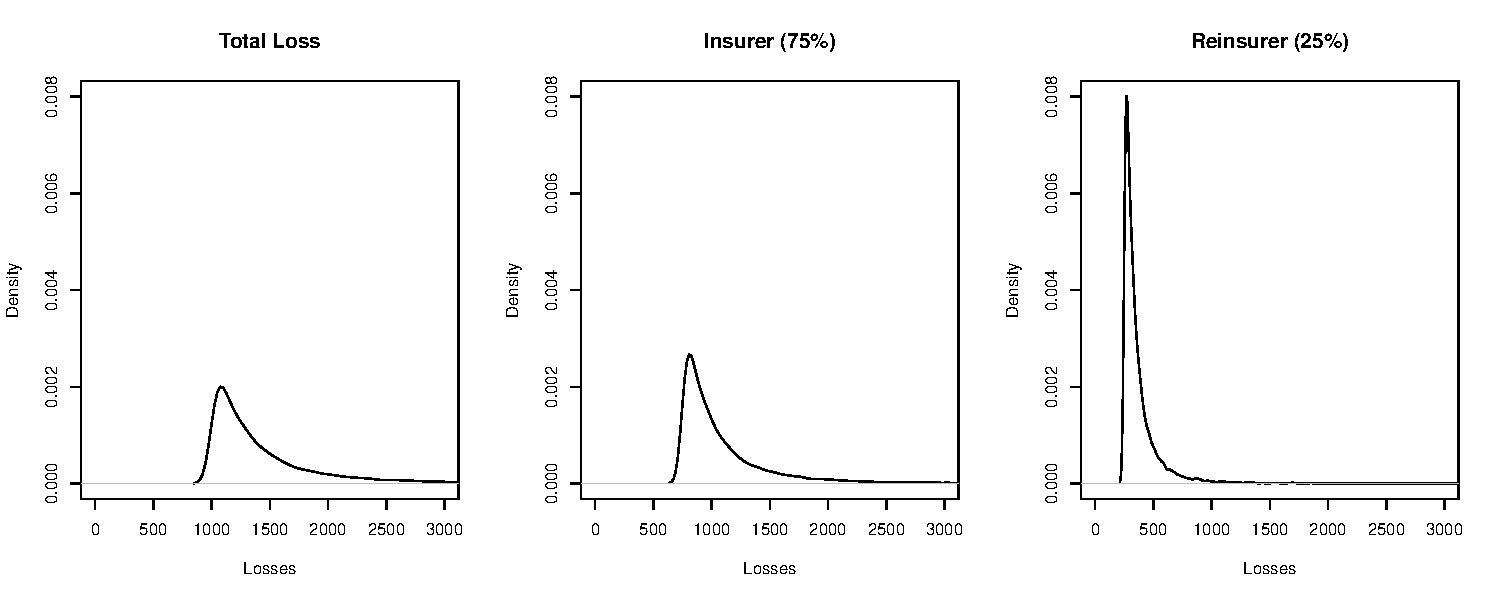
\includegraphics{LossDataAnalytics_files/figure-latex/unnamed-chunk-44-1} \end{center}

Mostrar el Código R

\hypertarget{toggleQuotaShare}{}
\begin{Shaded}
\begin{Highlighting}[]
\FunctionTok{set.seed}\NormalTok{(}\DecValTok{2018}\NormalTok{)}
\NormalTok{theta }\OtherTok{=} \DecValTok{1000}
\NormalTok{alpha }\OtherTok{=} \DecValTok{3}
\NormalTok{nSim }\OtherTok{=} \DecValTok{10000}
\FunctionTok{library}\NormalTok{(actuar)}
\NormalTok{X }\OtherTok{\textless{}{-}}  \FunctionTok{rpareto}\NormalTok{(nSim, }\AttributeTok{shape =}\NormalTok{ alpha, }\AttributeTok{scale =}\NormalTok{ theta)}

\FunctionTok{par}\NormalTok{(}\AttributeTok{mfrow=}\FunctionTok{c}\NormalTok{(}\DecValTok{1}\NormalTok{,}\DecValTok{3}\NormalTok{))}
\FunctionTok{plot}\NormalTok{(}\FunctionTok{density}\NormalTok{(X), }\AttributeTok{xlim=}\FunctionTok{c}\NormalTok{(}\DecValTok{0}\NormalTok{,}\DecValTok{3}\SpecialCharTok{*}\NormalTok{theta), }\AttributeTok{ylim=}\FunctionTok{c}\NormalTok{(}\DecValTok{0}\NormalTok{,}\FloatTok{0.008}\NormalTok{), }\AttributeTok{main=}\StringTok{"Total Loss"}\NormalTok{, }\AttributeTok{xlab=}\StringTok{"Losses"}\NormalTok{)}
\FunctionTok{plot}\NormalTok{(}\FunctionTok{density}\NormalTok{(}\FloatTok{0.75}\SpecialCharTok{*}\NormalTok{X), }\AttributeTok{xlim=}\FunctionTok{c}\NormalTok{(}\DecValTok{0}\NormalTok{,}\DecValTok{3}\SpecialCharTok{*}\NormalTok{theta), }\AttributeTok{ylim=}\FunctionTok{c}\NormalTok{(}\DecValTok{0}\NormalTok{,}\FloatTok{0.008}\NormalTok{), }\AttributeTok{main=}\StringTok{"Insurer (75\%)"}\NormalTok{, }\AttributeTok{xlab=}\StringTok{"Losses"}\NormalTok{)}
\FunctionTok{plot}\NormalTok{(}\FunctionTok{density}\NormalTok{(}\FloatTok{0.25}\SpecialCharTok{*}\NormalTok{X), }\AttributeTok{xlim=}\FunctionTok{c}\NormalTok{(}\DecValTok{0}\NormalTok{,}\DecValTok{3}\SpecialCharTok{*}\NormalTok{theta), }\AttributeTok{ylim=}\FunctionTok{c}\NormalTok{(}\DecValTok{0}\NormalTok{,}\FloatTok{0.008}\NormalTok{), }\AttributeTok{main=}\StringTok{"Reinsurer (25\%)"}\NormalTok{, }\AttributeTok{xlab=}\StringTok{"Losses"}\NormalTok{)}
\end{Highlighting}
\end{Shaded}

\hypertarget{el-cuota-parte-es-deseable-para-los-reaseguradores}{%
\subsubsection{El Cuota Parte es deseable para los Reaseguradores}\label{el-cuota-parte-es-deseable-para-los-reaseguradores}}

El contrato cuota parte es particularmente deseable para el reasegurador. Para entenderlo, supongamos que un asegurador y un reasegurador desean firmar un contrato para repartir las pérdidas totales \(X\) tal que \[Y_{asegurador}=g(X) \ \ \ \text{y} \ \ \ \ Y_{reasegurador}=X-g(X),\]
para alguna función genérica \(g(\cdot)\) (conocida como la función \emph{retención}). Supongamos además que el asegurador solo se preoucupa por la variabilidad de los siniestros retenidos y es indiferente a la elección de \(g\) siempre que \(Var(Y_{asegurador})\) sea la misma e igual, digamos, \(Q\). Entonces, el siguiente resultado demuestra que el contrato de reaseguro de cuota parte minimiza la incertidumbre del reasegurador medida por \(Var(Y_{reasegurador})\).

\textbf{Proposición}. Se supone que \(Var(Y_{asegurador})=Q.\) Entonces, \(Var ((1-c)X) \le Var(g(X))\) para todo \(g(.)\), donde \(c=Q/Var(X)\).

Mostrar la Justificación de la Proposición

\leavevmode\hypertarget{toggleProof}{}%
\textbf{Demostración de la Proposición}. Donde \(Y_{reasegurador} = X - Y_{asegurador}\) y la ley de la variación total

\[
\begin{array}{ll}
Var (Y_{reasegurador}) &= Var (X-Y_{asegurador}) \\
&= Var (X) + Var (Y_{asegurador})  - 2 Cov (X,Y_{asegurador}) \\
&=Var (X) + Q - 2 Corr (X,Y_{asegurador}) \times \sqrt{Q} \sqrt{Var (X)}
\end{array}
\]
En esta expresión, vemos que \(Q\) y \(Var(X)\) no cambian con la elección de \(g\). De este modo, se puede minimizar \(Var (Y_{reasegurador})\) maximizando la correlación \(Corr (X,Y_{asegurador})\). Si se usa un contrato de reaseguro cuota parte, entonces \(Corr (X,Y_{asegurador})=Corr (X,(1-c)X)=1\), la máxima correlación posible. Esto muestra la proposición.

\(\Box\)`

\begin{center}\rule{0.5\linewidth}{0.5pt}\end{center}

La propuesta es intuitivamente atractiva -- con un contrato de cuota parte, el reasegurador comparte la responsabilidad para siniestros muy grandes en la cola de la distribución. Esto contrasta con los acuerdos no proporcionales donde los reaseguradores se responsabilizan de las grandes reclamaciones.

\hypertarget{optimizando-los-contratos-cuota-parte-para-aseguradores}{%
\subsubsection{Optimizando los Contratos Cuota Parte para Aseguradores}\label{optimizando-los-contratos-cuota-parte-para-aseguradores}}

Ahora se asumen \(n\) riesgos en la cartera, \(X_1, \ldots, X_n,\) tal que la suma de la cartera es \(X= X_1 + \cdots + X_n\). Por simplicidad, nos centramos en el caso de riesgos independientes. Se considera una variación del contrato básico de cuota parte donde la cantidad retenida por el asegurador puede variar con cada riesgo, digamos \(c_i\). De este modo, la parte que el asegurador asume del riesgo de la cartera es \(Y_{asegurador} = \sum_{i=1}^n c_i X_i\). ¿Cuál es la mejor elección de las partes \(c_i\)?

Para formalizar esta pregunta, tratamos de encontrar aquellos valores de \(c_i\) que minimizan \(Var (Y_{asegurador})\) teniendo en cuenta la restricción de que \(E (Y_{asegurador}) = K.\) El requisito de que \(E (Y_{asegurador}) = K\) sugiere que los aseguradores prefieren retener un ingreso como mínimo de la cantidad de la constante \(K\). Sujeto a esta restricción sobre el ingreso, el asegurador prefiere minimizar la incertidumbre de los riesgos retenidos medida por la varianza.

Mostrar las Proporciones de Retención Óptimas

\leavevmode\hypertarget{toggleDerivationProof}{}%
\textbf{Las Proporciones de Retención Óptimas}

La minimización de \(Var(Y_{asegurador})\) sujeta a \(E(Y_{asegurador}) = K\) es un problema de optimización restringida -- se puede usar el método de los multiplicadores de Lagrange, una técnica de cálculo, para resolverlo. Para ello, se define el Lagrangiano

\[
\begin{array}{ll}
L &= Var (Y_{asegurador}) - \lambda (E (Y_{asegurador}) - K) \\
&= \sum_{i=1}^n c_i^2 ~Var(X_i) - \lambda (\sum_{i=1}^n c_i ~E(X_i) - K) 
\end{array}
\]
Calculando la derivada parcial respecto a \(\lambda\) y fijándola igual a cero simplemente significa que se fuerza la restricción, \(E(Y_{asegurador}) = K\), y se tienen que elegir las proporciones \(c_i\) para satisfacer esta restricción. Además, obteniendo la derivada parcial respecto a cada proporción \(c_i\) se obtiene
\[
\frac{\partial}{\partial c_i} L = 2 c_i ~Var(X_i) - \lambda ~E(X_i) = 0 
\]

Tal que

\[
c_i  =  \frac{\lambda}{2} \frac{E(X_i)}{Var(X_i)} .
\]
Con la restricción, se puede determinar \(\lambda\) como la solución de

\[
\begin{array}{ll}
K &= \sum_{i=1}^3 c_i \mathrm{E}(X_i) \\
&= \frac{\lambda}{2} \sum_{i=1}^3 \frac{\mathrm{E}(X_i)^2}{Var(X_i)} 
\end{array}
\]
Y usar este valor de \(\lambda\) para determinar las proporciones.

\begin{center}\rule{0.5\linewidth}{0.5pt}\end{center}

Desde el punto de vista matemático, se observa que la constante para el riesgo \(i\)th, \(c_i\) es proporcional a \(\frac{E(X_i)}{Var (X_i)}\). Esto es intuitivamente interesante. Si el resto permanece igual, un mayor ingreso medido por \(E (X_i)\) significa un valor más alto de \(c_i\). De la misma forma, un mayor grado de incertidumbre medido por \(Var(X_i)\)significa un menor valor de \(c_i\). El factor de escala proporcional se determina por el requisito de ingreso \(E(Y_{asegurador}) = K\). El siguiente ejemplo ayuda a entender esta relación.

\textbf{Ejemplo 10.3.2. Tres riesgos Pareto.} Se consideran tres riesgos que siguen una distribución de Pareto. Generar un gráfico, y el código necesario, que proporcionan valores de \(c_1\), \(c_2\), y \(c_3\) para un ingreso determinado \(K\). Observar si esos valores aumentan linealmente con \(K\).

Mostrar un Ejemplo con Tres Riesgos Pareto

\hypertarget{toggleParetoRisksProp}{}
\begin{Shaded}
\begin{Highlighting}[]
\NormalTok{theta1 }\OtherTok{=} \DecValTok{1000}\NormalTok{; theta2 }\OtherTok{=} \DecValTok{2000}\NormalTok{; theta3 }\OtherTok{=} \DecValTok{3000}\NormalTok{;}
\NormalTok{alpha1 }\OtherTok{=} \DecValTok{3}\NormalTok{; alpha2 }\OtherTok{=} \DecValTok{3}\NormalTok{; alpha3 }\OtherTok{=} \DecValTok{4}\NormalTok{;}
\FunctionTok{library}\NormalTok{(actuar)}
\NormalTok{propnfct }\OtherTok{\textless{}{-}} \ControlFlowTok{function}\NormalTok{(alpha,theta)\{}
\NormalTok{  mu    }\OtherTok{\textless{}{-}} \FunctionTok{mpareto}\NormalTok{(}\AttributeTok{shape=}\NormalTok{alpha, }\AttributeTok{scale=}\NormalTok{theta, }\AttributeTok{order=}\DecValTok{1}\NormalTok{)}
\NormalTok{  var   }\OtherTok{\textless{}{-}} \FunctionTok{mpareto}\NormalTok{(}\AttributeTok{shape=}\NormalTok{alpha, }\AttributeTok{scale=}\NormalTok{theta, }\AttributeTok{order=}\DecValTok{2}\NormalTok{) }\SpecialCharTok{{-}}\NormalTok{ mu}\SpecialCharTok{\^{}}\DecValTok{2}
\NormalTok{  mu}\SpecialCharTok{/}\NormalTok{var}
\NormalTok{\}}
\NormalTok{temp }\OtherTok{\textless{}{-}} \FunctionTok{propnfct}\NormalTok{(alpha1, theta1)}\SpecialCharTok{*}\FunctionTok{mpareto}\NormalTok{(}\AttributeTok{shape=}\NormalTok{alpha1, }\AttributeTok{scale=}\NormalTok{theta1, }\AttributeTok{order=}\DecValTok{1}\NormalTok{)}\SpecialCharTok{+}
        \FunctionTok{propnfct}\NormalTok{(alpha2, theta2)}\SpecialCharTok{*}\FunctionTok{mpareto}\NormalTok{(}\AttributeTok{shape=}\NormalTok{alpha2, }\AttributeTok{scale=}\NormalTok{theta2, }\AttributeTok{order=}\DecValTok{1}\NormalTok{)}\SpecialCharTok{+}
        \FunctionTok{propnfct}\NormalTok{(alpha3, theta3)}\SpecialCharTok{*}\FunctionTok{mpareto}\NormalTok{(}\AttributeTok{shape=}\NormalTok{alpha3, }\AttributeTok{scale=}\NormalTok{theta3, }\AttributeTok{order=}\DecValTok{1}\NormalTok{)  }
\NormalTok{KVec }\OtherTok{\textless{}{-}} \FunctionTok{seq}\NormalTok{(}\DecValTok{100}\NormalTok{, }\DecValTok{2500}\NormalTok{, }\AttributeTok{length.out=}\DecValTok{20}\NormalTok{)}
\NormalTok{Lambdavec }\OtherTok{\textless{}{-}} \DecValTok{2}\SpecialCharTok{*}\NormalTok{KVec}\SpecialCharTok{/}\NormalTok{temp}
\NormalTok{c1 }\OtherTok{\textless{}{-}} \FunctionTok{propnfct}\NormalTok{(alpha1, theta1)}
\NormalTok{c2 }\OtherTok{\textless{}{-}} \FunctionTok{propnfct}\NormalTok{(alpha2, theta2)}
\NormalTok{c3 }\OtherTok{\textless{}{-}} \FunctionTok{propnfct}\NormalTok{(alpha3, theta3)}
\NormalTok{c1Vec }\OtherTok{\textless{}{-}}\NormalTok{ c2Vec }\OtherTok{\textless{}{-}}\NormalTok{ c3Vec }\OtherTok{\textless{}{-}} \DecValTok{0}\SpecialCharTok{*}\NormalTok{KVec }
\ControlFlowTok{for}\NormalTok{ (j }\ControlFlowTok{in} \DecValTok{1}\SpecialCharTok{:}\DecValTok{20}\NormalTok{) \{}
\NormalTok{  c1Vec[j] }\OtherTok{\textless{}{-}}\NormalTok{ (Lambdavec[j]}\SpecialCharTok{/}\DecValTok{2}\NormalTok{) }\SpecialCharTok{*} \FunctionTok{propnfct}\NormalTok{(alpha1, theta1)}
\NormalTok{  c2Vec[j] }\OtherTok{\textless{}{-}}\NormalTok{ (Lambdavec[j]}\SpecialCharTok{/}\DecValTok{2}\NormalTok{) }\SpecialCharTok{*} \FunctionTok{propnfct}\NormalTok{(alpha2, theta2)}
\NormalTok{  c3Vec[j] }\OtherTok{\textless{}{-}}\NormalTok{ (Lambdavec[j]}\SpecialCharTok{/}\DecValTok{2}\NormalTok{) }\SpecialCharTok{*} \FunctionTok{propnfct}\NormalTok{(alpha3, theta3)}
\NormalTok{  \}}
\FunctionTok{plot}\NormalTok{(KVec, c1Vec, }\AttributeTok{type=}\StringTok{"l"}\NormalTok{, }\AttributeTok{ylab=}\StringTok{"proportion"}\NormalTok{, }\AttributeTok{xlab=}\StringTok{"required revenue (K)"}\NormalTok{, }\AttributeTok{ylim=}\FunctionTok{c}\NormalTok{(}\DecValTok{0}\NormalTok{,}\DecValTok{1}\NormalTok{))}
\FunctionTok{lines}\NormalTok{(KVec, c2Vec)}
\FunctionTok{lines}\NormalTok{(KVec, c3Vec)}
\FunctionTok{text}\NormalTok{(}\DecValTok{1200}\NormalTok{,}\FloatTok{0.80}\NormalTok{, }\FunctionTok{expression}\NormalTok{(c[}\DecValTok{1}\NormalTok{]))}
\FunctionTok{text}\NormalTok{(}\DecValTok{2000}\NormalTok{,}\FloatTok{0.75}\NormalTok{, }\FunctionTok{expression}\NormalTok{(c[}\DecValTok{2}\NormalTok{]))}
\FunctionTok{text}\NormalTok{(}\DecValTok{1500}\NormalTok{,}\FloatTok{0.30}\NormalTok{, }\FunctionTok{expression}\NormalTok{(c[}\DecValTok{3}\NormalTok{]))}
\end{Highlighting}
\end{Shaded}

\begin{center}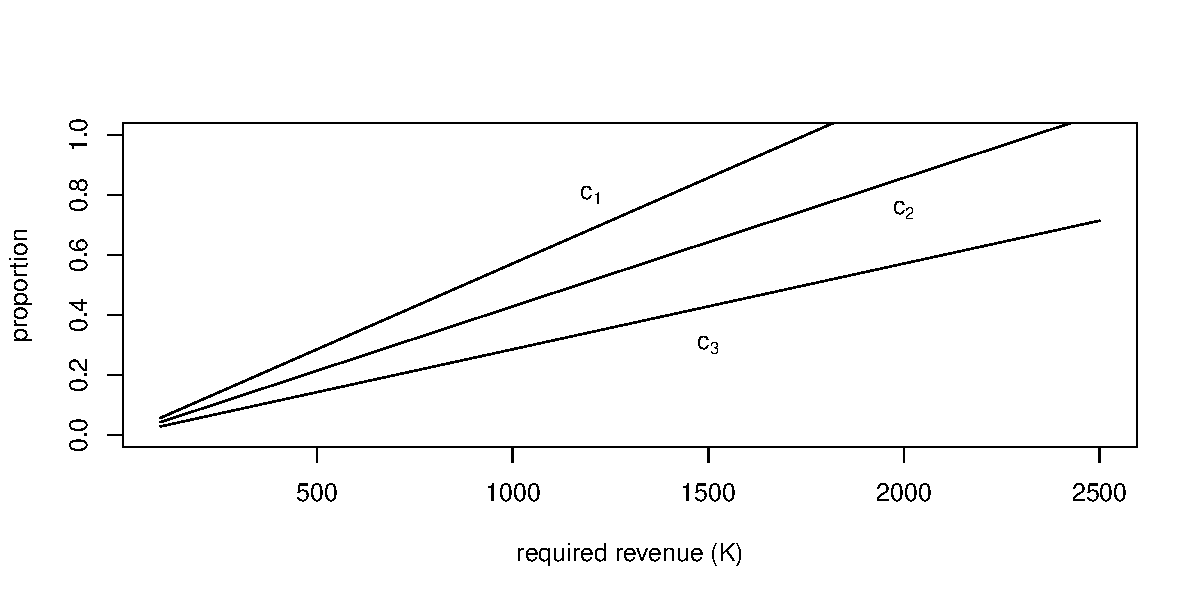
\includegraphics{LossDataAnalytics_files/figure-latex/unnamed-chunk-46-1} \end{center}

\hypertarget{S:NonProportionalRe}{%
\subsection{Reaseguro No-Proporcional}\label{S:NonProportionalRe}}

\hypertarget{la-optimalidad-del-seguro-stop-loss}{%
\subsubsection{La Optimalidad del Seguro Stop-Loss}\label{la-optimalidad-del-seguro-stop-loss}}

Bajo un contrato \textbf{stop-loss}, el asegurador establece un nivel de retención \(M (>0)\) y paga en su totalidad los siniestros para los que \(X \le M\). Además, para los siniestros con \(X > M\), el asegurador de directo paga \(M\) y el reasegurador para la cantidad restante \(X-M\). De este modo, el asegurador retiene una cantidad \(M\) del riesgo. Resumiendo, las cantidades pagadas por el asegurador de directo y el reasegurador son

\[
Y_{asegurador} =
\begin{cases}
X & \text{for } X \le M\\
M & \text{for } X >M \\
\end{cases} \ \ \ \ = \min(X,M) = X \wedge M
\]

y

\[
Y_{reasegurador} =
\begin{cases}
0 & \text{for } X \le M\\
X- M &  \text{for } X >M \\
\end{cases} \ \ \ \  = \max(0,X-M) .
\]

Como antes, notar que \(Y_{asegurador}+Y_{reasegurador}=X\).

El tipo de contrato stop-loss es particularmente deseable para el asegurador. Similar a lo visto anteriormente, se supone que un asegurador y un reasegurador desean establecer un contrato tal que \(Y_{asegurador}=g(X)\) e \(Y_{reasegurador}=X-g(X)\) para alguna función de retención genérica \(g(\cdot)\). Se supone además que el asegurador solo se encarga de la variabilidad de los siniestros retenidos y es indiferente respecto a la elección de \(g\) siempre que la \(Var(Y_{asegurador})\) pueda ser minimizada. De nuevo, se impone la restricción de que \(E(Y_{asegurador}) = K\); el asegurador tiene que retener un ingreso \(K\). Sujeto a esta restricción de ingreso, el asegurador desea minimizar la incertidumbre de los riesgos retenidos (medida por la varianza). Entonces, se obtiene el siguiente resultado que indica que el acuerdo de reaseguro stop-loss minimiza la incertidumbre del reasegurador medida por \(Var(Y_{reasegurador})\).

\textbf{Proposición}. Se supone que \(E(Y_{asegurador})=K.\) Entonces, \(Var (X \wedge M) \le Var(g(X))\) para todo \(g(.)\), donde \(M\) es tal que \(E(X \wedge M)=K\).

Mostrar la Justificación de la Proposición

\leavevmode\hypertarget{toggleProofStopLoss}{}%
\textbf{Demostración de la Proposición}. Añadir y restar una constante \(M\) y generar el cuadrado
\[
\begin{array}{ll}
Var(g(X)) &= E (g(X) - K)^2 = E (g(X) -M +M- K)^2 \\
&= E (g(X) -M)^2 +  (M- K)^2 +2 E (g(X) -M)(M- K) \\
&= E (g(X) -M)^2 -  (M- K)^2 ,
\end{array}
\]
Porque \(E(g(X))= K.\)

Ahora, para cualquier función de retención, se tiene \(g(X) \le X\), es decir, los siniestros retenidos por el asegurador son menores o iguales que el total de los siniestros. Usando la notación \(g_{SL}(X) = X \wedge M\) para los seguros stop-loss, se tiene

\[
\begin{array}{ll}
M- g_{SL}(X) &= M-(X \wedge M) \\
&= (M-X) \wedge 0 \\
&\le (M-g(X)) \wedge 0 .
\end{array}
\]
Elevando al cuadrado cada parte se tiene\\
\[(M- g_{SL}(X))^2 \le (M-g(X))^2 \wedge 0 \le (M-g(X))^2.\]

Volviendo a la expresión de la varianza,
\[
\begin{array}{ll}
Var(g_{SL}(X)) &= E (g_{SL}(X) -M)^2 -  (M- K)^2 \\
&\le E (g(X) -M)^2 -  (M- K)^2 = Var(g(X)) ,
\end{array}
\]
para cualquier función de retención \(g\). Esto demuestra la proposición.

\(\Box\)`

La proposición es intuitivamente interesante -- con el seguro stop-loss, el reasegurador es responsable de los siniestros muy grandes en la cola de la distribución, no el asegurador.

\hypertarget{exceso-de-puxe9rdida}{%
\subsubsection{Exceso de Pérdida}\label{exceso-de-puxe9rdida}}

Una forma cerrada de reaseguro no-proporcional es la cobertura \emph{exceso de pérdida} {Bajo un acuerdo de exceso de pérdida, el asegurador establece un nivel de retención para cada siniestro y paga indemnizaciones inferiores a dicho nivel con el reasegurador pagando el exceso}. Bajo este contrato, se asume que el riesgo total \(X\) puede entenderse como una composición de \(n\) riesgos separados \(X_1, \ldots, X_n\) y que cada uno de esos riesgos están sujetos a un límite superior, digamos, \(M_i\). De este modo el asegurador retiene

\[
Y_{i,asegurador} = X_i \wedge M_i \ \ \ \ Y_{asegurador} = \sum_{i=1}^n Y_{i,asegurador}
\]
y el reasegurador es responsable del exceso, \(Y_{reasegurador}=X - Y_{asegurador}\). Los límites de retención pueden variar según el riesgo o pueden ser los mismos para todos los riesgos, \(M_i =M\), para todo \(i\).

\hypertarget{elecciuxf3n-uxf3ptima-de-los-luxedmites-de-retenciuxf3n-para-exceso-de-puxe9rdidas}{%
\subsubsection{Elección Óptima de los Límites de Retención para Exceso de Pérdidas}\label{elecciuxf3n-uxf3ptima-de-los-luxedmites-de-retenciuxf3n-para-exceso-de-puxe9rdidas}}

¿Cuál es la mejor elección de los límites de retención del exceso de pérdidas \(M_i\)? Para formalizar esta pregunta, se propone encontrar aquellos valores de \(M_i\) que minimizan \(Var(Y_{asegurador})\) sujetos a la restricción de que \(E(Y_{asegurador}) = K.\) Sujeto a esta restricción de ingresos, el asegurador desea minimizar la incertidumbre de los riesgos retenidos (medidos por la varianza).

Mostrar las Proporciones de Retención Óptimas

\leavevmode\hypertarget{toggleDerivationProofExcess}{}%
\textbf{Los Límites de Retención Óptimos}

Minimizar \(Var(Y_{asegurador})\) sujeto a \(E(Y_{asegurador}) = K\) es un problema de optimización restringida -- se puede usar el método de los multiplicadores de Lagrange, una técnica de cálculo, para resolverlo. Como antes, se define el Lagrangiano
\[
\begin{array}{ll}
L &= Var (Y_{asegurador}) - \lambda (E(Y_{asegurador}) - K) \\
&= \sum_{i=1}^n ~Var (X_i \wedge M_i) - \lambda (\sum_{i=1}^n ~E(X_i \wedge M_i)- K).
\end{array}
\]

En primer lugar se presentan las relaciones

\[
E(X \wedge M) = \int_0^M ~(1- F(x))dx
\]
y

\[
E(X \wedge M)^2 = 2\int_0^M ~x(1- F(x))dx.
\]

Calculando la derivada parcial respecto a \(\lambda\) y fijándola igual a cero simplemente significa que se fuerza la restricción, \(E(Y_{asegurador}) = K\), y se han de elegir los límites \(M_i\) para satisfacer dicha restricción. Además, calculando la derivada parcial respecto a cada límite \(M_i\) se obtiene

\[
\begin{array}{ll}
\frac{\partial}{\partial M_i} L 
&= \frac{\partial}{\partial M_i}  ~Var(X_i \wedge M_i)  - \lambda \frac{\partial}{\partial M_i} ~E(X_i \wedge M_i) \\
&= \frac{\partial}{\partial M_i} \left(E(X_i \wedge M_i)^2 -(E(X_i \wedge M_i))^2\right) - \lambda (1-F_i(M_i)) \\
&= 2 M_i (1-F_i(M_i)) - 2 E(X_i \wedge M_i) (1-F_i(M_i))-
\lambda (1-F_i(M_i)).
\end{array}
\]

Estableciendo \(\frac{\partial}{\partial M_i} L =0\) y resolviendo para \(\lambda\), se obtiene

\[
\lambda = 2 (M_i - E(X_i \wedge M_i)) .
\]

Desde el punto de vista matemático se obtiene que el límite de retención menos los siniestros esperados por el asegurador, \(M_i - E(X_i \wedge M_i)\), es el mismo para \emph{todos} los riesgos. Esto es intuitivamente interesante.

\textbf{Ejemplo 10.3.3. Exceso de pérdidas para tres riesgos de Pareto .} Se consideran tres riesgos que siguen una distribución de Pareto, cada uno definido por un set diferente de parámetros (de forma que son independientes pero no-idénticos). Demostrar numéricamente que los límites óptimos de retención \(M_1\), \(M_2\), y \(M_3\) calulados como los límites de retención menos los siniestros esperados por el asegurador, \(M_i - E(X_i \wedge M_i)\), son los mismos para todos los riesgos, como se demuestra teóricamente. Además, comparar gráficamente la distribución de todos los riesgos con la de los retenidos por el asegurador y el reasegurador.

Mostrar un Ejemplo con Tres Riesgos Pareto

\leavevmode\hypertarget{toggleParetoRisksExcess}{}%
Primero se optimiza el Lagrangiano usando el paquete \texttt{R} \texttt{alabama} para \emph{Algoritmo de Minimización de la Barrera Adaptativa del Lagrangiano Aumentado}.

\begin{Shaded}
\begin{Highlighting}[]
\NormalTok{theta1 }\OtherTok{=} \DecValTok{1000}\NormalTok{;theta2 }\OtherTok{=} \DecValTok{2000}\NormalTok{;theta3 }\OtherTok{=} \DecValTok{3000}\NormalTok{;}
\NormalTok{alpha1 }\OtherTok{=} \DecValTok{3}\NormalTok{;   alpha2 }\OtherTok{=} \DecValTok{3}\NormalTok{;   alpha3 }\OtherTok{=} \DecValTok{4}\NormalTok{;}
\NormalTok{Pmin }\OtherTok{\textless{}{-}} \DecValTok{2000}
\FunctionTok{library}\NormalTok{(actuar)}
\NormalTok{VarFct }\OtherTok{\textless{}{-}} \ControlFlowTok{function}\NormalTok{(M)\{}
\NormalTok{  M1}\OtherTok{=}\NormalTok{M[}\DecValTok{1}\NormalTok{];M2}\OtherTok{=}\NormalTok{M[}\DecValTok{2}\NormalTok{];M3}\OtherTok{=}\NormalTok{M[}\DecValTok{3}\NormalTok{]}
\NormalTok{  mu1    }\OtherTok{\textless{}{-}} \FunctionTok{levpareto}\NormalTok{(}\AttributeTok{limit=}\NormalTok{M1,}\AttributeTok{shape=}\NormalTok{alpha1, }\AttributeTok{scale=}\NormalTok{theta1, }\AttributeTok{order=}\DecValTok{1}\NormalTok{)}
\NormalTok{  var1   }\OtherTok{\textless{}{-}} \FunctionTok{levpareto}\NormalTok{(}\AttributeTok{limit=}\NormalTok{M1,}\AttributeTok{shape=}\NormalTok{alpha1, }\AttributeTok{scale=}\NormalTok{theta1, }\AttributeTok{order=}\DecValTok{2}\NormalTok{)}\SpecialCharTok{{-}}\NormalTok{mu1}\SpecialCharTok{\^{}}\DecValTok{2}
\NormalTok{  mu2    }\OtherTok{\textless{}{-}} \FunctionTok{levpareto}\NormalTok{(}\AttributeTok{limit=}\NormalTok{M2,}\AttributeTok{shape=}\NormalTok{alpha2, }\AttributeTok{scale=}\NormalTok{theta2, }\AttributeTok{order=}\DecValTok{1}\NormalTok{)}
\NormalTok{  var2   }\OtherTok{\textless{}{-}} \FunctionTok{levpareto}\NormalTok{(}\AttributeTok{limit=}\NormalTok{M2,}\AttributeTok{shape=}\NormalTok{alpha2, }\AttributeTok{scale=}\NormalTok{theta2, }\AttributeTok{order=}\DecValTok{2}\NormalTok{)}\SpecialCharTok{{-}}\NormalTok{mu2}\SpecialCharTok{\^{}}\DecValTok{2}
\NormalTok{  mu3    }\OtherTok{\textless{}{-}} \FunctionTok{levpareto}\NormalTok{(}\AttributeTok{limit=}\NormalTok{M3,}\AttributeTok{shape=}\NormalTok{alpha3, }\AttributeTok{scale=}\NormalTok{theta3, }\AttributeTok{order=}\DecValTok{1}\NormalTok{)}
\NormalTok{  var3   }\OtherTok{\textless{}{-}} \FunctionTok{levpareto}\NormalTok{(}\AttributeTok{limit=}\NormalTok{M3,}\AttributeTok{shape=}\NormalTok{alpha3, }\AttributeTok{scale=}\NormalTok{theta3, }\AttributeTok{order=}\DecValTok{2}\NormalTok{)}\SpecialCharTok{{-}}\NormalTok{mu3}\SpecialCharTok{\^{}}\DecValTok{2}
\NormalTok{  varFct }\OtherTok{\textless{}{-}}\NormalTok{ var1 }\SpecialCharTok{+}\NormalTok{var2}\SpecialCharTok{+}\NormalTok{var3}
\NormalTok{  meanFct }\OtherTok{\textless{}{-}}\NormalTok{ mu1}\SpecialCharTok{+}\NormalTok{mu2}\SpecialCharTok{+}\NormalTok{mu3}
  \FunctionTok{c}\NormalTok{(meanFct,varFct)}
\NormalTok{  \}}
\NormalTok{f }\OtherTok{\textless{}{-}} \ControlFlowTok{function}\NormalTok{(M)\{}\FunctionTok{VarFct}\NormalTok{(M)[}\DecValTok{2}\NormalTok{]\}}
\NormalTok{h }\OtherTok{\textless{}{-}} \ControlFlowTok{function}\NormalTok{(M)\{}\FunctionTok{VarFct}\NormalTok{(M)[}\DecValTok{1}\NormalTok{] }\SpecialCharTok{{-}}\NormalTok{ Pmin\}}
\FunctionTok{library}\NormalTok{(alabama)}
\NormalTok{par0}\OtherTok{=}\FunctionTok{rep}\NormalTok{(}\DecValTok{1000}\NormalTok{,}\DecValTok{3}\NormalTok{)}
\NormalTok{op }\OtherTok{\textless{}{-}} \FunctionTok{auglag}\NormalTok{(}\AttributeTok{par=}\NormalTok{par0,}\AttributeTok{fn=}\NormalTok{f,}\AttributeTok{hin=}\NormalTok{h,}\AttributeTok{control.outer=}\FunctionTok{list}\NormalTok{(}\AttributeTok{trace=}\ConstantTok{FALSE}\NormalTok{))}
\end{Highlighting}
\end{Shaded}

Los límites de retención óptimos \(M_1\), \(M_2\), y \(M_3\) calculados como los límites de retención menos los siniestros esperados del asegurador, \(M_i - E(X_i \wedge M_i)\), son los mismos para todos los riesgos, como se ha derivado teóricamente.

\begin{Shaded}
\begin{Highlighting}[]
\NormalTok{M1star }\OtherTok{=}\NormalTok{ op}\SpecialCharTok{$}\NormalTok{par[}\DecValTok{1}\NormalTok{];M2star }\OtherTok{=}\NormalTok{ op}\SpecialCharTok{$}\NormalTok{par[}\DecValTok{2}\NormalTok{];M3star }\OtherTok{=}\NormalTok{ op}\SpecialCharTok{$}\NormalTok{par[}\DecValTok{3}\NormalTok{]}
\NormalTok{M1star }\SpecialCharTok{{-}}\FunctionTok{levpareto}\NormalTok{(M1star,}\AttributeTok{shape=}\NormalTok{alpha1, }\AttributeTok{scale=}\NormalTok{theta1,}\AttributeTok{order=}\DecValTok{1}\NormalTok{)}
\end{Highlighting}
\end{Shaded}

\begin{verbatim}
[1] 1344.135
\end{verbatim}

\begin{Shaded}
\begin{Highlighting}[]
\NormalTok{M2star }\SpecialCharTok{{-}}\FunctionTok{levpareto}\NormalTok{(M2star,}\AttributeTok{shape=}\NormalTok{alpha2, }\AttributeTok{scale=}\NormalTok{theta2,}\AttributeTok{order=}\DecValTok{1}\NormalTok{)}
\end{Highlighting}
\end{Shaded}

\begin{verbatim}
[1] 1344.133
\end{verbatim}

\begin{Shaded}
\begin{Highlighting}[]
\NormalTok{M3star }\SpecialCharTok{{-}}\FunctionTok{levpareto}\NormalTok{(M3star,}\AttributeTok{shape=}\NormalTok{alpha3, }\AttributeTok{scale=}\NormalTok{theta3,}\AttributeTok{order=}\DecValTok{1}\NormalTok{)}
\end{Highlighting}
\end{Shaded}

\begin{verbatim}
[1] 1344.133
\end{verbatim}

Gráficamente se compara la distribución de los riesgos totales con los retenidos por el asegurador y el reasegurador.

\begin{Shaded}
\begin{Highlighting}[]
\FunctionTok{set.seed}\NormalTok{(}\DecValTok{2018}\NormalTok{)}
\NormalTok{nSim }\OtherTok{=} \DecValTok{10000}
\FunctionTok{library}\NormalTok{(actuar)}
\NormalTok{Y1 }\OtherTok{\textless{}{-}} \FunctionTok{rpareto}\NormalTok{(nSim, }\AttributeTok{shape =}\NormalTok{ alpha1, }\AttributeTok{scale =}\NormalTok{ theta1)}
\NormalTok{Y2 }\OtherTok{\textless{}{-}} \FunctionTok{rpareto}\NormalTok{(nSim, }\AttributeTok{shape =}\NormalTok{ alpha2, }\AttributeTok{scale =}\NormalTok{ theta2)}
\NormalTok{Y3 }\OtherTok{\textless{}{-}} \FunctionTok{rpareto}\NormalTok{(nSim, }\AttributeTok{shape =}\NormalTok{ alpha3, }\AttributeTok{scale =}\NormalTok{ theta3)}
\NormalTok{YTotal }\OtherTok{\textless{}{-}}\NormalTok{ Y1 }\SpecialCharTok{+}\NormalTok{ Y2 }\SpecialCharTok{+}\NormalTok{ Y3}
\NormalTok{Yinsur }\OtherTok{\textless{}{-}}  \FunctionTok{pmin}\NormalTok{(Y1,M1star)}\SpecialCharTok{+}\FunctionTok{pmin}\NormalTok{(Y2,M2star)}\SpecialCharTok{+}\FunctionTok{pmin}\NormalTok{(Y3,M3star)}
\NormalTok{Yreinsur }\OtherTok{\textless{}{-}}\NormalTok{ YTotal }\SpecialCharTok{{-}}\NormalTok{ Yinsur}

\FunctionTok{par}\NormalTok{(}\AttributeTok{mfrow=}\FunctionTok{c}\NormalTok{(}\DecValTok{1}\NormalTok{,}\DecValTok{3}\NormalTok{))}
\FunctionTok{plot}\NormalTok{(}\FunctionTok{density}\NormalTok{(YTotal),   }\AttributeTok{xlim=}\FunctionTok{c}\NormalTok{(}\DecValTok{0}\NormalTok{,}\DecValTok{10000}\NormalTok{), }\AttributeTok{main=}\StringTok{"Total Loss"}\NormalTok{, }\AttributeTok{xlab=}\StringTok{"Losses"}\NormalTok{)}
\FunctionTok{plot}\NormalTok{(}\FunctionTok{density}\NormalTok{(Yinsur),   }\AttributeTok{xlim=}\FunctionTok{c}\NormalTok{(}\DecValTok{0}\NormalTok{,}\DecValTok{10000}\NormalTok{), }\AttributeTok{main=}\StringTok{"Insurer"}\NormalTok{,    }\AttributeTok{xlab=}\StringTok{"Losses"}\NormalTok{)}
\FunctionTok{plot}\NormalTok{(}\FunctionTok{density}\NormalTok{(Yreinsur), }\AttributeTok{xlim=}\FunctionTok{c}\NormalTok{(}\DecValTok{0}\NormalTok{,}\DecValTok{10000}\NormalTok{), }\AttributeTok{main=}\StringTok{"Reinsurer"}\NormalTok{,  }\AttributeTok{xlab=}\StringTok{"Losses"}\NormalTok{)}
\end{Highlighting}
\end{Shaded}

\begin{center}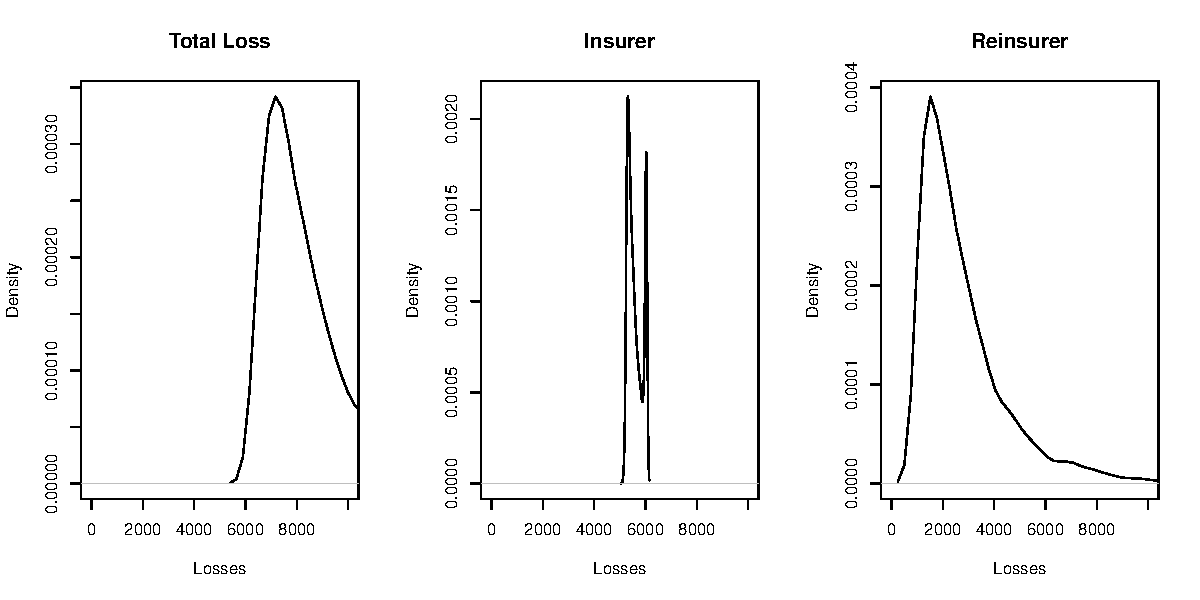
\includegraphics{LossDataAnalytics_files/figure-latex/unnamed-chunk-49-1} \end{center}

\begin{center}\rule{0.5\linewidth}{0.5pt}\end{center}

\hypertarget{S:AdditionalRe}{%
\subsection{Acuerdos de Reaseguro Adicionales}\label{S:AdditionalRe}}

\hypertarget{acuerdo-surplus-share-proportional-treaty}{%
\subsubsection{Acuerdo Surplus Share Proportional Treaty}\label{acuerdo-surplus-share-proportional-treaty}}

Otro acuerdo proporcional es el denominado \emph{surplus share}{Un acuerdo de reaseguro proporcional que es frecuente en seguros de daños comerciales. Un acuerdo surplus share permite al reasegurado limitar su exposición en un determinado riesgo a una cantidad dada (el pleno de retención). El reasegurador asume una parte del riesgo en proporción a la cantidad que el valor asegurado excede el pleno de retención, hasta un límite dado (expresado como un múltiplo del pleno de retención, o número de plenos).}; este tipo de contratos es frecuente en seguros de daños comerciales.

\begin{itemize}
\tightlist
\item
  Un acuerdo surplus share permite al reasegurado limitar su exposición a un determinado riesgo a una cantidad dada (el \emph{pleno de retención}).
\item
  El reasegurador asume una parte del riesgo en proporción a la cantidad que el valor asegurado excede el pleno de retención, hasta un límite dado (expresado como un múltiplo del pleno de retención, o número de plenos).
\end{itemize}

Por ejemplo, sea el pleno de retención 100,000 y el límite 4 veces el pleno (400,000). Entonces, si \(X\) es la pérdida, la parte del reasegurador es \(\min(400000, (X-100000)_+)\).

\hypertarget{layers-de-cobertura}{%
\subsubsection{Layers de cobertura}\label{layers-de-cobertura}}

Se pueden extender los acuerdos de reaseguro no-proporcionales stop-loss introduiendo partes adicionales al contrato. Por ejemplo, en lugar de simplemente un asegurador y un reasegurador o un asegurador y un tomador, pensar en una situación con las tres partes, tomador, asegurador, y reasegurador, los cuales se ponen de acuerdo en como repartir el riesgo. De forma más general, se consideran \(k\) partes. Si \(k=3\), podria tratarse de un asegurador y dos reaseguradores diferentes.

\textbf{Ejemplo 10.3.4. Layers de cobertura para tres partes.}

\begin{itemize}
\item
  Se supone que hay \(k=3\) partes. La primera parte es responsable de los siniestros hasta 100, la segunda es responsable de los siniestros entre 100 y 3000, y la tercera es responsable de los siniestros por encima de 3000.
\item
  Si hay cuatro siniestros de cuantías 50, 600, 1800 y 4000, entonces estarían repartidos entre las partes de la forma:
\end{itemize}

\begin{longtable}[]{@{}lllllr@{}}
\toprule
Layer & Siniestro 1 & Siniestro 2 & Siniestro 3 & Siniestro 4 & Total \\
\midrule
\endhead
(0, 100{]} & 50 & 100 & 100 & 100 & 350 \\
(100, 3000{]} & 0 & 500 & 1700 & 2900 & 5100 \\
(3000, \(\infty\)) & 0 & 0 & 0 & 1000 & 1000 \\
Total & 50 & 600 & 1800 & 4000 & 6450 \\
\bottomrule
\end{longtable}

\begin{center}\rule{0.5\linewidth}{0.5pt}\end{center}

Para considerar la situación general con \(k\) grupos, se divide la línea de los reales positivos en \(k\) intervalos usando los puntos de corte
\[0 = M_0 < M_1 < \cdots < M_{k-1} < M_k = \infty.\]

Observar que el intervalo \(j\)th es \((M_{j-1}, M_j]\). Ahora sea \(Y_j\) la cuantía de riesgo compartida por la parte \(j\)th. Para ilustrarlo, si una pérdida \(x\) es tal que \(M_{j-1} <x \le M_j\), entonces
\[\left(\begin{array}{c}
    Y_1\\ Y_2 \\ \vdots \\ Y_j \\Y_{j+1} \\ \vdots \\Y_k
    \end{array}\right)
    =\left(\begin{array}{c}
    M_1-M_0 \\ M_2-M_1  \\ \vdots \\ x-M_{j-1}  \\ 0 \\ \vdots \\0
    \end{array}\right)\]

De forma más clara, podemos escribir
\[Y_j = \min(X,M_j) - \min(X,M_{j-1}) .\]

Con la expresión \(Y_j = \min(X,M_j) - \min(X,M_{j-1})\), se observa que la parte \(j\)th es responsable de los siniestros en el intervalo \((M_{j-1}, M_j].\) Con esto, es fàcil comprobar que \(X = Y_1 + Y_2 + \cdots + Y_k.\) Como se destaca en el siguiente ejemplo, también se puede remarcar que las partes no necesitan ser diferentes.

\textbf{Ejemplo 10.3.5.}
- Suponer que un tomador es responsable de los primeros 500 y todos los siniestros en exceso de 100.000. El asegurador coge siniestros entre 100 y 100.000.
- Entonces, se deberían usar \(M_1 = 100\), \(M_2 =100000\).
- El tomador es responsable de \(Y_1 =\min(X,100)\) y
\(Y_3 = X - \min(X,100000) = \max(0, X-100000)\).

Para saber más, consultar en \href{https://sites.google.com/a/wisc.edu/local-government-property-insurance-fund/home/reinsurance}{Wisconsin Property Fund site} un ejemplo de layers de reaseguro.

\hypertarget{ejemplo-de-gestiuxf3n-de-cartera}{%
\subsubsection{Ejemplo de Gestión de Cartera}\label{ejemplo-de-gestiuxf3n-de-cartera}}

Pueden encontrarse muchas otras variaciones de los contratos originales. Para tener más ilustraciones, se considera lo siguiente.

\textbf{Ejemplo. 10.3.6. Gestión de carteras.} Tú eres el jefe de riesgos de una empresa de telecomunicaciones. Tu empresa tiene varios riesgos de daños y responsabilidad. Se considera:

\begin{itemize}
\tightlist
\item
  \(X_1\) - edificios, modelizados por medio de una distribución gamma de media 200 y parámetro de escala 100.
\item
  \(X_2\) - vehículos a motor, modelizados usando una distribución gamma con media 400 y parámetro de escala 200.
\item
  \(X_3\) - responsabilidad de directores y ejecutivos, modelizada usando una distribución de Pareto con media 1000 y parámetro de escala 1000.
\item
  \(X_4\) - ciberriesgos, modelizados usando una distribución de Pareto con media 1000 y parámetro de escala 2000.
\end{itemize}

Se describe el riesgo total como \[X = X_1 + X_2 + X_3 + X_4 .\]

Por simplicidad, se asume que esos riesgos son independientes.

Para controlar el riesgo, se contrata algún tipo de cobertura aseguradora. Se puede preferir controlar internamente pequeñas cantidades relacionades con edificios y vehículos a motor, hasta \(M_1\) y \(M_2\), respectivamente. Se recurre al seguro para cubrir todos los demás riesgos. Específicamente, la parte del asegurador es
\[ Y_{asegurador} = (X_1 - M_1)_+ + (X_2 - M_2)_+ + X_3 + X_4 ,\]
De forma que tu riesgo retenido es \(Y_{retenido}= X- Y_{asegurador} =\) \(\min(X_1,M_1) + \min(X_2,M_2)\). Usando franquicias \(M_1=\) 100 y \(M_2=\) 200:

\begin{enumerate}
\def\labelenumi{\alph{enumi}.}
\tightlist
\item
  Determinar de la cuantía esperada por siniestro (i)la retenida, (ii) la aceptada por el asegurador, y (iii) la cuantía total.
\item
  Determinar los percentiles 80, 90, 95, y 99 para (i) la parte retenida, (ii) la parte aceptada por el asegurador, y (iii) la cuantía total.
\item
  Comparar las distribuciones graficando las densidades para (i) la parte retenida, (ii) la aceptada por el asegurador, y (iii) la cuantía total.
\end{enumerate}

Mostrar Solución al Ejemplo con Código R

\leavevmode\hypertarget{togglePortMgtExample}{}%
En preparación, se adjunta el código necesario para establecer los parámetros.

\begin{Shaded}
\begin{Highlighting}[]
\CommentTok{\# Para la distribución gamma, usar}
\NormalTok{alpha1 }\OtherTok{\textless{}{-}} \DecValTok{2}\NormalTok{;      theta1 }\OtherTok{\textless{}{-}} \DecValTok{100}
\NormalTok{alpha2 }\OtherTok{\textless{}{-}} \DecValTok{2}\NormalTok{;      theta2 }\OtherTok{\textless{}{-}} \DecValTok{200}
\CommentTok{\# Para la distribución de Pareto, usar}
\NormalTok{alpha3 }\OtherTok{\textless{}{-}} \DecValTok{2}\NormalTok{;      theta3 }\OtherTok{\textless{}{-}} \DecValTok{1000}
\NormalTok{alpha4 }\OtherTok{\textless{}{-}} \DecValTok{3}\NormalTok{;      theta4 }\OtherTok{\textless{}{-}} \DecValTok{2000}
\CommentTok{\# Límites}
\NormalTok{M1     }\OtherTok{\textless{}{-}} \DecValTok{100}
\NormalTok{M2     }\OtherTok{\textless{}{-}} \DecValTok{200}
\end{Highlighting}
\end{Shaded}

Con estos parámetros, se pueden simular acaecimientos de los riesgos de la cartera.

\begin{Shaded}
\begin{Highlighting}[]
\CommentTok{\# Simular los riesgos}
\NormalTok{nSim }\OtherTok{\textless{}{-}} \DecValTok{10000}  \CommentTok{\#número de simulaciones}
\FunctionTok{set.seed}\NormalTok{(}\DecValTok{2017}\NormalTok{) }\CommentTok{\#establecer la seed para reproducir el trabajo }
\NormalTok{X1 }\OtherTok{\textless{}{-}} \FunctionTok{rgamma}\NormalTok{(nSim,alpha1,}\AttributeTok{scale =}\NormalTok{ theta1)  }
\NormalTok{X2 }\OtherTok{\textless{}{-}} \FunctionTok{rgamma}\NormalTok{(nSim,alpha2,}\AttributeTok{scale =}\NormalTok{ theta2)  }
\CommentTok{\# Para la Distribución de Pareto, usar}
\FunctionTok{library}\NormalTok{(actuar)}
\NormalTok{X3 }\OtherTok{\textless{}{-}} \FunctionTok{rpareto}\NormalTok{(nSim,}\AttributeTok{scale=}\NormalTok{theta3,}\AttributeTok{shape=}\NormalTok{alpha3)}
\NormalTok{X4 }\OtherTok{\textless{}{-}} \FunctionTok{rpareto}\NormalTok{(nSim,}\AttributeTok{scale=}\NormalTok{theta4,}\AttributeTok{shape=}\NormalTok{alpha4)}
\CommentTok{\# Riesgos de Cartera}
\NormalTok{X         }\OtherTok{\textless{}{-}}\NormalTok{ X1 }\SpecialCharTok{+}\NormalTok{ X2 }\SpecialCharTok{+}\NormalTok{ X3 }\SpecialCharTok{+}\NormalTok{ X4}
\NormalTok{Yretenido }\OtherTok{\textless{}{-}} \FunctionTok{pmin}\NormalTok{(X1,M1) }\SpecialCharTok{+} \FunctionTok{pmin}\NormalTok{(X2,M2)}
\NormalTok{Yasegurador  }\OtherTok{\textless{}{-}}\NormalTok{ X }\SpecialCharTok{{-}}\NormalTok{ Yretenido}
\end{Highlighting}
\end{Shaded}

\textbf{(a)} Aquí está el código para las cantidades esperadas por siniestro.

\begin{Shaded}
\begin{Highlighting}[]
\CommentTok{\# Cantidades esperadas por siniestro}
\NormalTok{ExpVec }\OtherTok{\textless{}{-}} \FunctionTok{t}\NormalTok{(}\FunctionTok{as.matrix}\NormalTok{(}\FunctionTok{c}\NormalTok{(}\FunctionTok{mean}\NormalTok{(Yretenido),}\FunctionTok{mean}\NormalTok{(Yasegurador),}\FunctionTok{mean}\NormalTok{(X))))}
\FunctionTok{colnames}\NormalTok{(ExpVec) }\OtherTok{\textless{}{-}} \FunctionTok{c}\NormalTok{(}\StringTok{"Retenido"}\NormalTok{, }\StringTok{"Asegurador"}\NormalTok{,}\StringTok{"Total"}\NormalTok{)}
\FunctionTok{round}\NormalTok{(ExpVec,}\AttributeTok{digits=}\DecValTok{2}\NormalTok{)}
\end{Highlighting}
\end{Shaded}

\begin{verbatim}
     Retenido Asegurador   Total
[1,]   269.05    5274.41 5543.46
\end{verbatim}

\textbf{(b)} Aquí está el código para los cuantiles.

\begin{Shaded}
\begin{Highlighting}[]
\CommentTok{\# Cuantiles}
\NormalTok{quantMat }\OtherTok{\textless{}{-}} \FunctionTok{rbind}\NormalTok{(}
  \FunctionTok{quantile}\NormalTok{(Yretenido, }\AttributeTok{probs=}\FunctionTok{c}\NormalTok{(}\FloatTok{0.80}\NormalTok{, }\FloatTok{0.90}\NormalTok{, }\FloatTok{0.95}\NormalTok{, }\FloatTok{0.99}\NormalTok{)),}
  \FunctionTok{quantile}\NormalTok{(Yasegurador,  }\AttributeTok{probs=}\FunctionTok{c}\NormalTok{(}\FloatTok{0.80}\NormalTok{, }\FloatTok{0.90}\NormalTok{, }\FloatTok{0.95}\NormalTok{, }\FloatTok{0.99}\NormalTok{)),}
  \FunctionTok{quantile}\NormalTok{(X       ,  }\AttributeTok{probs=}\FunctionTok{c}\NormalTok{(}\FloatTok{0.80}\NormalTok{, }\FloatTok{0.90}\NormalTok{, }\FloatTok{0.95}\NormalTok{, }\FloatTok{0.99}\NormalTok{)))}
\FunctionTok{rownames}\NormalTok{(quantMat) }\OtherTok{\textless{}{-}} \FunctionTok{c}\NormalTok{(}\StringTok{"Retenido"}\NormalTok{, }\StringTok{"Asegurador"}\NormalTok{,}\StringTok{"Total"}\NormalTok{)}
\FunctionTok{round}\NormalTok{(quantMat,}\AttributeTok{digits=}\DecValTok{2}\NormalTok{)}
\end{Highlighting}
\end{Shaded}

\begin{verbatim}
               80%     90%     95%      99%
Retenido    300.00  300.00  300.00   300.00
Asegurador 6075.67 7399.80 9172.69 14859.02
Total      6351.35 7675.04 9464.20 15159.02
\end{verbatim}

\textbf{(c)} Aquí está el código para los gráficos de densidades del riesgo retenido, del asegurador y el total de riesgo de cartera.

\begin{Shaded}
\begin{Highlighting}[]
\FunctionTok{par}\NormalTok{(}\AttributeTok{mfrow=}\FunctionTok{c}\NormalTok{(}\DecValTok{1}\NormalTok{,}\DecValTok{3}\NormalTok{))}
\FunctionTok{plot}\NormalTok{(}\FunctionTok{density}\NormalTok{(Yretenido), }\AttributeTok{xlim=}\FunctionTok{c}\NormalTok{(}\DecValTok{0}\NormalTok{,}\DecValTok{500}\NormalTok{), }\AttributeTok{main=}\StringTok{"Riesgo de Cartera Retenido"}\NormalTok{, }\AttributeTok{xlab=}\StringTok{"Pérdida (Tener en cuenta la escala horizontal diferente)"}\NormalTok{, }\AttributeTok{ylab =} \StringTok{"Densidad (Tener en cuenta la diferente escala vertical)"}\NormalTok{)}
\FunctionTok{plot}\NormalTok{(}\FunctionTok{density}\NormalTok{(Yasegurador), }\AttributeTok{xlim=}\FunctionTok{c}\NormalTok{(}\DecValTok{0}\NormalTok{,}\DecValTok{15000}\NormalTok{), }\AttributeTok{main=}\StringTok{"Riesgo de Cartera del Asegurador"}\NormalTok{, }\AttributeTok{xlab=}\StringTok{"Pérdida"}\NormalTok{)}
\FunctionTok{plot}\NormalTok{(}\FunctionTok{density}\NormalTok{(X), }\AttributeTok{xlim=}\FunctionTok{c}\NormalTok{(}\DecValTok{0}\NormalTok{,}\DecValTok{15000}\NormalTok{), }\AttributeTok{main=}\StringTok{"Riesgo Total de Cartera"}\NormalTok{, }\AttributeTok{xlab=}\StringTok{"Pérdida"}\NormalTok{)}
\end{Highlighting}
\end{Shaded}

\begin{center}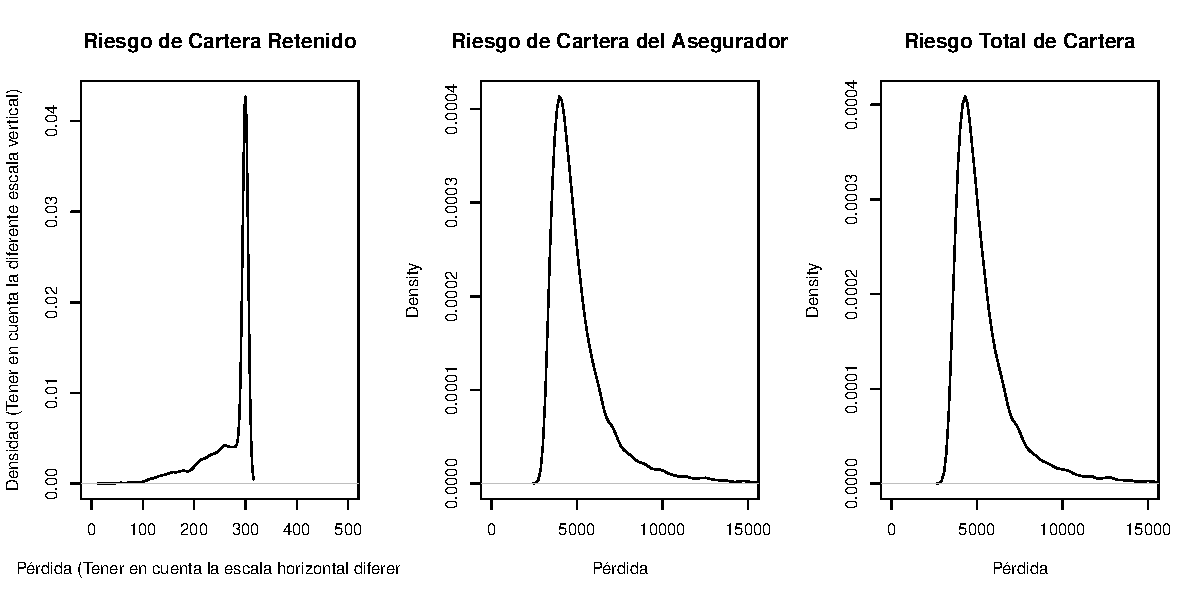
\includegraphics{LossDataAnalytics_files/figure-latex/unnamed-chunk-55-1} \end{center}

\hypertarget{recursos-y-colaboradores-adicionales}{%
\section{Recursos y Colaboradores adicionales}\label{recursos-y-colaboradores-adicionales}}

\begin{itemize}
\tightlist
\item
  \textbf{Edward W. (Jed) Frees}, University of Wisconsin-Madison, y \textbf{Jianxi Su}, Purdue University son los autores principales de la versión inicial de este capítulo. Email: \href{mailto:jfrees@bus.wisc.edu}{\nolinkurl{jfrees@bus.wisc.edu}} y/o \href{mailto:jianxi@purdue.edu}{\nolinkurl{jianxi@purdue.edu}} para comentarios sobre el capítulo y mejoras sugeridas.
\item
  Revisores del Capítulo: Fei Huang, Hirokazu (Iwahiro) Iwasawa, Peng Shi, Ping Wang, Chengguo Weng.
\item
  Traducción al español: Mercedes Ayuso (Universitat de Barcelona)
\end{itemize}

Algunos de los ejemplos de este capítulo se tomaron de \citet{clark1996basics}, \citet{klugman2012}, y \citet{bahnemann2015distributions}. Estas referencias proporcionan excelentes Fuentes para discusiones adicionales y ejemplos.

\hypertarget{C:LossReserves}{%
\chapter{Provisiones}\label{C:LossReserves}}

\emph{Vista Previa del Capítulo.} Este capítulo introduce las provisiones (también conocidas como reservas por pérdidas) para seguros de propiedad y accidentes (P\&C, según sus siglas en inglés, o generales, no-vida). En particular, el capítulo presenta algunas herramientas analíticas básicas esenciales para evaluar las reservas de una cartera de productos de seguros de P\&C. En primer lugar, la Sección \ref{S:motivation} motiva la necesidad de las provisiones. Después la Sección \ref{S:Data} estudia las fuentes de datos disponibles e introduce algunas notaciones formales para enfocar las provisiones como un desafío de predicción. A continuación, la sección \ref{S:Chain-ladder} cubre el método de chain-ladder y el modelo de chain-ladder con distribución libre de Mack. La sección \ref{S:GLMs} finalmente desarrolla un enfoque totalmente estocástico para determinar la reserva pendiente con modelos lineales generalizados (GLMs, según sus siglas en inglés), incluyendo la técnica de bootstrapping para obtener una distribución predictiva de la reserva pendiente a través de la simulación.

\hypertarget{S:motivation}{%
\section{Motivación}\label{S:motivation}}

Nuestro punto de partida es la vida de un siniestro en un seguro de P\&C. La figura \ref{fig:tikz-run-off} muestra el desarrollo del siniestro a lo largo del tiempo e identifica los eventos de interés:

\begin{figure}

{\centering \includegraphics{LossDataAnalytics_files/figure-latex/tikz-run-off-1} 

}

\caption{Vida o run-off de un siniestro}\label{fig:tikz-run-off}
\end{figure}

El evento asegurado o accidente ocurre en el momento \(t_{occ}\). Este siniestro es reportado a la compañía de seguros en el momento \(t_{rep}\), después de un cierto tiempo de demora. Si la compañía de seguros acepta la reclamación presentada, realizará diferentes pagos para reembolsar la pérdida financiera del titular de la póliza. En este ejemplo, la compañía de seguros compensa la pérdida sufrida con pagos por pérdidas en los momentos \(t_1\), \(t_2\) u \(t_3\). Finalmente, la reclamación se liquida o cierra en el momento \(t_{set}\).

A menudo las reclamaciones no se liquidan inmediatamente debido a la presencia de una demora en la presentación de la reclamación, un retraso en el proceso de liquidación o ambos. El retraso en la notificación es el tiempo que transcurre entre la ocurrencia del evento asegurado y la notificación de este evento a la compañía de seguros. El tiempo entre la notificación y la liquidación de una reclamación se conoce como la demora en la liquidación. Por ejemplo, es muy intuitivo que una reclamación por daños materiales se resuelve más rápidamente que una reclamación por lesiones corporales que impliquen un tipo de lesión compleja. Las reclamaciones cerradas pueden reabrirse debido a nuevos acontecimientos, por ejemplo, una lesión que requiere un tratamiento adicional. En conjunto, el desarrollo del siniestro requiere un tiempo. La presencia de este retraso en la tramitación de un siniestro obliga al asegurador a disponer de capital para liquidar estas reclamaciones en el futuro.

\hypertarget{S:claim-types}{%
\subsection{Siniestros cerrados, IBNR, y RBNS}\label{S:claim-types}}

Basándonos en el estado de la liquidación de la reclamación, distinguimos tres tipos de siniestros en los libros de una compañía de seguros. El primer tipo de siniestro es una reclamación cerrada. Para estos siniestros se ha observado el desarrollo completo. Con la línea roja de la figura \ref{fig:tikz-closed} que indica el momento presente, todos los eventos del desarrollo del siniestro tienen lugar antes del momento presente. Por lo tanto, estos eventos se observan en el momento actual. Por comodidad, asumiremos que una reclamación cerrada no puede reabrirse.

\begin{figure}

{\centering \includegraphics{LossDataAnalytics_files/figure-latex/tikz-closed-1} 

}

\caption{Vida de un siniestro cerrado}\label{fig:tikz-closed}
\end{figure}

Un siniestro RBNS ha sido comunicado pero no está completamente liquidado (\textbf{R}eported \textbf{B}ut \textbf{N}ot \textbf{S}ettled) en el momento actual o en el momento de la evaluación, es decir, el momento en que las provisiones deben ser calculadas y reservadas por el asegurador. La ocurrencia, la notificación y posiblemente algunos pagos tienen lugar antes del momento presente, pero el cierre del siniestro ocurre en el futuro, más allá del momento presente.

\begin{figure}

{\centering \includegraphics{LossDataAnalytics_files/figure-latex/tikz-RBNS-1} 

}

\caption{Vida de un siniestro RBNS}\label{fig:tikz-RBNS}
\end{figure}

Un siniestro IBNR ha ocurrido en el pasado pero aún no ha sido comunicado (\textbf{I}ncurred \textbf{B}ut \textbf{N}ot yet \textbf{R}eported). El evento asegurado ocurrió, pero la compañía de seguros aún no está al tanto del siniestro asociado. Esta reclamación se comunicará en el futuro y su desarrollo completo (desde la comunicación hasta la liquidación) tendrá lugar en el futuro.

\begin{figure}

{\centering \includegraphics{LossDataAnalytics_files/figure-latex/tikz-IBNR-1} 

}

\caption{Vida de un siniestro IBNR}\label{fig:tikz-IBNR}
\end{figure}

Las compañías de seguros provisionarán el capital para cumplir con sus responsabilidades futuras con respecto a los siniestros tanto RBNS como IBNR. El desarrollo futuro de tales siniestros es incierto y se utilizarán técnicas de modelización predictiva para calcular las reservas adecuadas, a partir de los datos históricos de desarrollo observados en siniestros similares.

\hypertarget{por-quuxe9-reservar}{%
\subsection{¿Por qué reservar?}\label{por-quuxe9-reservar}}

El ciclo de producción invertido del mercado de los seguros y la dinámica de los siniestros que se muestra en la sección \ref{S:claim-types} motivan la necesidad de reservar y el diseño de herramientas de modelización predictiva para estimar las reservas. En los seguros, los ingresos por primas preceden a los costes. Un asegurador cobrará una prima a un cliente, antes de saber realmente cómo de costosa será la póliza o el contrato de seguro. En la industria manufacturera normalmente no es así y el fabricante sabe - antes de vender un producto - cuál fue el coste de producción de este producto. En un momento de evaluación específico \(\tau\) el asegurador predecirá sus responsabilidades pendientes con respecto a los contratos vendidos en el pasado. Esta es la reserva de siniestros o reserva para pérdidas; es el capital necesario para liquidar los siniestros abiertos de exposiciones pasadas. Es un elemento muy importante en el balance del asegurador, más concretamente en el pasivo de este balance.

\hypertarget{S:Data}{%
\section{Datos de provisiones}\label{S:Data}}

\hypertarget{de-micro-a-macro}{%
\subsection{De Micro a Macro}\label{de-micro-a-macro}}

Ahora analizamos los datos disponibles para estimar la reserva pendiente de una cartera de contratos P\&C. Las compañías de seguros suelen registrar los datos sobre el desarrollo de un siniestro individual como se muestra en la línea de tiempo a la izquierda de la figura \ref{fig:tikz-micro-macro}. Nos referimos a los datos registrados a este nivel como \textbf{datos granulares o de micro-nivel}. Típicamente, un actuario agrega la información registrada sobre la evolución individual de los siniestros para todas las reclamaciones de una cartera. Esta agregación da lugar a datos estructurados en un formato triangular como se muestra en la parte derecha de la figura \ref{fig:tikz-micro-macro}. Estos datos se denominan datos \textbf{agregados o a nivel macro} porque cada celda del triángulo muestra la información obtenida al agregar el desarrollo de múltiples reclamaciones.

\begin{figure}

{\centering \includegraphics{LossDataAnalytics_files/figure-latex/tikz-micro-macro-1} 

}

\caption{De datos granulares a triángulo de desarrollo}\label{fig:tikz-micro-macro}
\end{figure}

La visualización triangular utilizada en la provisión por pérdidas se llama triángulo \textbf{run-off o de desarrollo}. En el eje vertical el triángulo enumera los años de accidente o de ocurrencia durante los cuales se sigue una cartera. Los pagos provisionados para un siniestro específico están conectados con el año durante el cual ocurrió el evento asegurado. En el eje horizontal se indica el retraso en el pago desde la ocurrencia del evento asegurado.

\hypertarget{triuxe1ngulos-de-desarrollo}{%
\subsection{Triángulos de desarrollo}\label{triuxe1ngulos-de-desarrollo}}

Un primer ejemplo de un triángulo de desarrollo con pagos incrementales se muestra en la Figura \ref{fig:tikz-triangle} (tomada de \citet{WuthrichMerz2008}, Tabla 2.2, también utilizada en \citet{WuthrichMerz2015}, Tabla 1.4). Los años de los accidentes (o años de ocurrencia) se muestran en el eje vertical y van desde 2004 hasta 2013. Se refieren al año durante el cual ocurrió el evento asegurado. El eje horizontal indica el retraso en el pago en años desde la ocurrencia del evento asegurado. \emph{0 retraso} se utiliza para los pagos realizados en el año de ocurrencia del accidente o evento asegurado. \emph{Un año} de retraso se utiliza para los pagos realizados en el año posterior a la ocurrencia del accidente.

\begin{figure}

{\centering \includegraphics{LossDataAnalytics_files/figure-latex/tikz-triangle-1} 

}

\caption{Triángulo de Desarrollo con datos de pagos incrementales. Fuente: @WuthrichMerz2008, Tabla 2.2.}\label{fig:tikz-triangle}
\end{figure}

Por ejemplo, la celda \((2004, 0)\) del triángulo anterior muestra el número \(5947\), la cantidad total pagada en el año 2004 por todas los siniestros ocurridos en el año 2004. Por lo tanto, es la cantidad total pagada con 0 años de retraso en todas las reclamaciones que ocurrieron en el año 2004. De manera similar, el número de la celda \((2012,1)\) muestra el total de \(2357,9\) pagados en el año 2013 por todos los siniestros que ocurrieron en el año 2012.

\begin{figure}

{\centering \includegraphics{LossDataAnalytics_files/figure-latex/tikz-cum-triangle-1} 

}

\caption{ Triángulo de desarrollo con datos de pago acumulados. Fuente: @WuthrichMerz2008, Tabla 2.2.}\label{fig:tikz-cum-triangle}
\end{figure}

Mientras que el triángulo de la Figura \ref{fig:tikz-triangle} muestra los datos de pago incremental, la Figura \ref{fig:tikz-cum-triangle} muestra la misma información en formato acumulado. Ahora, la celda \((2004,1)\) muestra la cantidad total pagada \emph{hasta} la demora de pago 1 para todos los siniestros que ocurrieron en el año 2004. Por lo tanto, es la suma de la cantidad pagada en 2004 y la cantidad pagada en 2005 por los accidentes que ocurrieron en 2004.

Se pueden utilizar diferentes datos en triángulos de desarrollo como los que se muestran en la Figura \ref{fig:tikz-triangle} y en la Figura \ref{fig:tikz-cum-triangle}. Dependiendo del tipo de datos utilizados, el triángulo se utilizará para estimar diferentes cantidades.

Por ejemplo, en el formato incremental una celda puede mostrar:

\begin{itemize}
\tightlist
\item
  los pagos de los siniestros, como explicado antes
\item
  el número de reclamaciones que se produjeron en un año específico y que se notificaron con cierto retraso, cuando el objetivo es estimar el número de siniestros IBNR
\item
  la variación en las cantidades incurridas, donde las cantidades incurridas de los siniestros son la suma de los siniestros pagados acumulados y las estimaciones individuales. La estimación individual es la estimación del tramitador de los siniestros sobre la cantidad pendiente de pago de un siniestro.
\end{itemize}

En el formato acumulado una celda puede mostrar:

\begin{itemize}
\tightlist
\item
  la cantidad pagada acumulada, según lo explicado antes
\item
  el número total de siniestros de un año de ocurrencia, notificados hasta un determinado retraso
\item
  las cantidades incurridas de los siniestros.
\end{itemize}

Es posible que se disponga de otras fuentes de información, por ejemplo, covariables (como el tipo de siniestros), información externa (como inflación, cambios regulatorios). La mayoría de los métodos de provisión de siniestros diseñados para los triángulos de desarrollo se basan más bien en una sola fuente de información, aunque algunas contribuciones recientes se centran en el uso de datos más detallados para la provisión de pérdidas.

\hypertarget{notaciuxf3n-de-provisiones}{%
\subsection{Notación de provisiones}\label{notaciuxf3n-de-provisiones}}

\hypertarget{triuxe1ngulos-de-desarrollo-1}{%
\subsubsection*{Triángulos de desarrollo}\label{triuxe1ngulos-de-desarrollo-1}}
\addcontentsline{toc}{subsubsection}{Triángulos de desarrollo}

Para formalizar lo mostrado en las figuras \ref{fig:tikz-triangle} y \ref{fig:tikz-cum-triangle}, permitimos que \(i\) se refiera al año de ocurrencia o accidente, el año en que ocurrió el evento asegurado. En nuestra anotación el primer año de accidente considerado en la cartera se denota con 1 y el último año de accidente, el más reciente, se denota con \(I\). De la misma forma, \(j\) se refiere al año de retraso de pago o desarrollo, donde un retraso igual a 0 corresponde al año de accidente. La figura \ref{fig:tikz-math-triangle} muestra un triángulo en el que se considera el mismo número de años en la dirección vertical y en la horizontal, por lo que \(j\) va desde 0 hasta \(J = I-1\).

\begin{figure}

{\centering \includegraphics{LossDataAnalytics_files/figure-latex/tikz-math-triangle-1} 

}

\caption{Notación matemática para un triángulo de desarrollo. Fuente: @WuthrichMerz2008}\label{fig:tikz-math-triangle}
\end{figure}

La variable aleatoria \(X_{ij}\) denota las reclamaciones incrementales pagadas en el período de desarrollo \(j\) de los siniestros del año de accidente \(i\). Por lo tanto, \(X_{ij}\) es la cantidad total pagada en el año de desarrollo \(j\) por todos los siniestros que ocurrieron en el año de ocurrencia \(i\). Estas cuantías se pagan realmente en el año contable o natural \(i+j\). Desde un punto de vista acumulado, \(C_{ij}\) es la cantidad acumulada pagada hasta (e incluyendo) el año de desarrollo \(j\) por los accidentes ocurridos en el año \(i\). Al final, se paga una cantidad total de \(C_{iJ}\) en el último año de desarrollo \(J\) por los siniestros ocurridos en el año de accidente \(i\). En este capítulo el tiempo se expresa en años, aunque también se pueden utilizar otras unidades de tiempo, por ejemplo, semestres o trimestres.

\hypertarget{provisiuxf3n-por-puxe9rdidas}{%
\subsubsection*{Provisión por pérdidas}\label{provisiuxf3n-por-puxe9rdidas}}
\addcontentsline{toc}{subsubsection}{Provisión por pérdidas}

En el momento de la evaluación \(\tau\), se han observado los datos del triángulo superior, mientras que el triángulo inferior tiene que predecirse. Aquí, el momento de la evaluación es el final del año del accidente \(I\) lo que implica que una celda \((i,j)\) con \(i+j \leq I\) se observa, y una celda \((i,j)\) con \(i+j > I\) pertenece al futuro y tiene que ser predicha. Así, para un triángulo de desarrollo acumulado, el objetivo de un método de provisión de pérdidas es predecir \(C_{i,I-1}\),
la cantidad última por los siniestros para el año de ocurrencia \(i\), correspondiente al período final de desarrollo \(I-1\) en la Figura \ref{fig:tikz-cum-triangle}. Asumimos que - más allá de este período - no habrá más pagos, aunque este supuesto puede relajarse.

Dado que \(C_{i,I-1}\) es acumulado, incluye tanto una parte observada como una parte que debe predecirse. Por lo tanto, la provisión por pagos pendientes para el año de accidente \(i\) es

\begin{eqnarray*}
\mathcal{R}^{(0)}_{i} = \sum_{\ell=I-i+1}^{I-1} X_{i\ell} = C_{i,I}-C_{i,I-i}.
\end{eqnarray*}

Expresamos la reserva como una suma de datos incrementales, \(X_{i\ell}\), o como la diferencia entre datos acumulados. En este último caso, la cantidad pendiente es la cantidad acumulada final \(C_{i,I}\) menos la cantidad acumulada observada más reciente \(C_{i,I-i}\). Siguiendo a \citet{WuthrichMerz2015}, la anotación \(\mathcal{R}^{(0)}_{i}\) se refiere a la reserva para el año de ocurrencia \(i\) donde \(i=1,\ldots,I\). El superíndice \((0)\) se refiere a la evaluación de la reserva en el momento actual, digamos \(\tau = 0\). Entendemos que \(\tau = 0\) al final del año de ocurrencia \(I\), el año calendario más reciente para el que se observan y registran los datos.

\hypertarget{S:Rcode}{%
\subsection{Código R para resumir datos de provisión de pérdidas}\label{S:Rcode}}

Usamos el paquete \texttt{ChainLadder} \citep{R-chainladder} para importar triángulos de desarrollo en \texttt{R} y para explorar las tendencias presentes en estos triángulos. La viñeta del paquete documenta muy bien sus funciones para trabajar con datos triangulares. Primero, exploramos dos formas de importar un triángulo.

\hypertarget{datos-con-formato-extenso}{%
\subsubsection*{Datos con formato extenso}\label{datos-con-formato-extenso}}
\addcontentsline{toc}{subsubsection}{Datos con formato extenso}

El conjunto de datos \texttt{triangle\_W\_M\_long.txt} almacena el triángulo de desarrollo acumulado de \citet{WuthrichMerz2008} (Tabla 2.2) en formato largo. Es decir, cada celda del triángulo es una fila de este conjunto de datos, y se almacenan tres características: la cuantía del pago (acumulado, en este ejemplo), el año de ocurrencia (\(i\)) y el retraso del pago (\(j\)). Importamos el archivo .txt y almacenamos el conjunto de datos resultante como \texttt{my\_triangle\_long}:

\begin{verbatim}
   payment origin dev
1  5946975   2004   0
2  9668212   2004   1
3 10563929   2004   2
4 10771690   2004   3
5 10978394   2004   4
6 11040518   2004   5
\end{verbatim}

Usamos la función \texttt{as.triangle} del paquete \texttt{ChainLadder} para transformar el conjunto de datos en formato triangular. El objeto resultante \texttt{my\_triangle} ahora es de tipo \texttt{triangle}.

\begin{verbatim}
 'triangle' int [1:10, 1:10] 5946975 6346756 6269090 5863015 5778885 6184793 5600184 5288066 5290793 5675568 ...
 - attr(*, "dimnames")=List of 2
  ..$ origin: chr [1:10] "2004" "2005" "2006" "2007" ...
  ..$ dev   : chr [1:10] "0" "1" "2" "3" ...
\end{verbatim}

Mostramos el triángulo y reconocemos los números (en miles) de la figura \ref{fig:tikz-cum-triangle}. Las celdas en el triángulo inferior se indican como valores ausentes (\emph{not available}), \texttt{NA}.

\begin{verbatim}
      dev
origin    0    1     2     3     4     5     6     7     8     9
  2004 5947 9668 10564 10772 10978 11041 11106 11121 11132 11148
  2005 6347 9593 10316 10468 10536 10573 10625 10637 10648    NA
  2006 6269 9245 10092 10355 10508 10573 10627 10636    NA    NA
  2007 5863 8546  9269  9459  9592  9681  9724    NA    NA    NA
  2008 5779 8524  9178  9451  9682  9787    NA    NA    NA    NA
  2009 6185 9013  9586  9831  9936    NA    NA    NA    NA    NA
  2010 5600 8493  9057  9282    NA    NA    NA    NA    NA    NA
  2011 5288 7728  8256    NA    NA    NA    NA    NA    NA    NA
  2012 5291 7649    NA    NA    NA    NA    NA    NA    NA    NA
  2013 5676   NA    NA    NA    NA    NA    NA    NA    NA    NA
\end{verbatim}

\hypertarget{datos-en-formato-triangular}{%
\subsubsection*{Datos en formato triangular}\label{datos-en-formato-triangular}}
\addcontentsline{toc}{subsubsection}{Datos en formato triangular}

Alternativamente, el triángulo puede ser almacenado en un archivo .csv con los años de ocurrencia en las filas y los años de desarrollo en las celdas de la columna. Importamos este archivo .csv y transformamos \texttt{my\_triangle\_csv} resultante en una matriz.

Inspeccionamos el triángulo:

\begin{verbatim}
      dev
origin    0    1     2     3     4     5     6     7     8     9
  2004 5947 9668 10564 10772 10978 11041 11106 11121 11132 11148
  2005 6347 9593 10316 10468 10536 10573 10625 10637 10648    NA
  2006 6269 9245 10092 10355 10508 10573 10627 10636    NA    NA
  2007 5863 8546  9269  9459  9592  9681  9724    NA    NA    NA
  2008 5779 8524  9178  9451  9682  9787    NA    NA    NA    NA
  2009 6185 9013  9586  9831  9936    NA    NA    NA    NA    NA
  2010 5600 8493  9057  9282    NA    NA    NA    NA    NA    NA
  2011 5288 7728  8256    NA    NA    NA    NA    NA    NA    NA
  2012 5291 7649    NA    NA    NA    NA    NA    NA    NA    NA
  2013 5676   NA    NA    NA    NA    NA    NA    NA    NA    NA
\end{verbatim}

\hypertarget{de-acumulado-a-incremental-y-viceversa}{%
\subsubsection*{De acumulado a incremental y viceversa}\label{de-acumulado-a-incremental-y-viceversa}}
\addcontentsline{toc}{subsubsection}{De acumulado a incremental y viceversa}

Las funciones de \texttt{R} \texttt{cum2incr()} y \texttt{incr2cum()} nos permiten pasar de datos acumulados a incrementales, y viceversa, de una manera fácil.

\begin{verbatim}
      dev
origin    0    1   2   3   4   5  6  7  8  9
  2004 5947 3721 896 208 207  62 66 15 11 16
  2005 6347 3246 723 152  68  37 53 11 12 NA
  2006 6269 2976 847 263 153  65 54  9 NA NA
  2007 5863 2683 723 191 133  88 43 NA NA NA
  2008 5779 2745 654 273 230 105 NA NA NA NA
  2009 6185 2828 573 245 105  NA NA NA NA NA
  2010 5600 2893 563 226  NA  NA NA NA NA NA
  2011 5288 2440 528  NA  NA  NA NA NA NA NA
  2012 5291 2358  NA  NA  NA  NA NA NA NA NA
  2013 5676   NA  NA  NA  NA  NA NA NA NA NA
\end{verbatim}

Reconocemos el triángulo incremental de la figura \ref{fig:tikz-triangle}.

\hypertarget{visualizaciuxf3n-de-triuxe1ngulos}{%
\subsubsection*{Visualización de triángulos}\label{visualizaciuxf3n-de-triuxe1ngulos}}
\addcontentsline{toc}{subsubsection}{Visualización de triángulos}

Para explorar la evolución de los pagos acumulados por año de ocurrencia, la figura \ref{fig:plottriangle} muestra \texttt{my\_triangle} usando la función \texttt{plot} disponible para los objetos de tipo \texttt{triangle} en el paquete \texttt{ChainLadder}. Cada línea de este gráfico muestra un año de ocurrencia (de 2004 a 2013, etiquetado como 1 a 10). Los períodos de desarrollo se etiquetan de 1 a 10 (en lugar de 0 a 9, como se usó anteriormente).

\begin{Shaded}
\begin{Highlighting}[]
\FunctionTok{plot}\NormalTok{(my\_triangle)}
\end{Highlighting}
\end{Shaded}

\begin{figure}

{\centering \includegraphics[width=0.8\linewidth]{LossDataAnalytics_files/figure-latex/plottriangle-1} 

}

\caption{Desarrollo del siniestro por año de ocurrencia }\label{fig:plottriangle}
\end{figure}

Alternativamente, el argumento \texttt{lattice} crea un gráfico por año de ocurrencia.

\begin{Shaded}
\begin{Highlighting}[]
\FunctionTok{plot}\NormalTok{(my\_triangle, }\AttributeTok{lattice =} \ConstantTok{TRUE}\NormalTok{)}
\end{Highlighting}
\end{Shaded}

\begin{center}\includegraphics[width=0.8\linewidth]{LossDataAnalytics_files/figure-latex/plot_triangle_lattice-1} \end{center}

En lugar de graficar el triángulo acumulado guardado en \texttt{my\_triangle}, podemos graficar el triángulo de desarollo incremental.

\begin{Shaded}
\begin{Highlighting}[]
\FunctionTok{plot}\NormalTok{(my\_triangle\_incr)}
\end{Highlighting}
\end{Shaded}

\begin{center}\includegraphics[width=0.8\linewidth]{LossDataAnalytics_files/figure-latex/plot_triangle_incr-1} \end{center}

\begin{Shaded}
\begin{Highlighting}[]
\FunctionTok{plot}\NormalTok{(my\_triangle\_incr, }\AttributeTok{lattice =} \ConstantTok{TRUE}\NormalTok{)}
\end{Highlighting}
\end{Shaded}

\begin{center}\includegraphics[width=0.8\linewidth]{LossDataAnalytics_files/figure-latex/plot_triangle_incr-2} \end{center}

\hypertarget{S:Chain-ladder}{%
\section{Chain-Ladder}\label{S:Chain-ladder}}

El método más utilizado para estimar las reservas por pagos pendientes es el llamado método chain-ladder. Los orígenes de este método no están claros pero se afianzó firmemente en aplicaciones prácticas a principios de los 70, \citet{taylor1986claims}. Como se mostrará, el nombre se refiere al encadenamiento (chain) de una secuencia de factores (desarrollo año a año) en una escalera (ladder) de factores; las pérdidas inmaduras suben hacia la madurez cuando se multiplican por esta concatenación de ratios, de ahí la descripción de \emph{método chain-ladder.} Empezaremos explorando el método chain-ladder en su versión determinista o algorítmica, por lo tanto sin hacer ninguna suposición estocástica. Luego describiremos el modelo chain-ladder de distribución libre de Mack.

\hypertarget{S:DeterministicCL}{%
\subsection{Chain-Ladder Determinista}\label{S:DeterministicCL}}

El método chain-ladder determinista se centra en el triángulo de desarrollo en forma acumulada. Recordemos que una celda \((i,j)\) en este triángulo muestra la cantidad acumulada pagada hasta el período de desarrollo \(j\) por siniestros que ocurrieron en el año \(i\). El método chain-ladder asume que los \textbf{factores de desarrollo} \(f_j\) (también llamados factores edad-a-edad, ratios de enlace o factores chain-ladder) existen de tal manera que

\[
C_{i,j+1} = f_j \times C_{i,j}.
\]

Por tanto, el factor de desarrollo indica cómo la cantidad acumulada en el año de desarrollo \(j\) crece hasta la cantidad acumulada en el año \(j+1\). Destacamos la cantidad acumulada en el período 0 en azul y la cantidad acumulada en el período 1 en rojo en la Figura \ref{fig:tikz-cum-triangle-cl1} tomada de \citet{WuthrichMerz2008} (Tabla 2.2, también utilizada en \citet{WuthrichMerz2015}, Tabla 1.4).

\begin{figure}

{\centering \includegraphics{LossDataAnalytics_files/figure-latex/tikz-cum-triangle-cl1-1} 

}

\caption{Triángulo de desarrollo con datos de pagos acumulados que muestra la cantidad acumulada en el período 0 en azul y la cantidad acumulada en el período 1 en rojo. Fuente: @WuthrichMerz2008, Tabla 2.2.}\label{fig:tikz-cum-triangle-cl1}
\end{figure}

El método chain-ladder presenta una forma intuitiva para estimar o calcular estos factores de desarrollo. Dado que el primer factor de desarrollo \(f_0\) describe el desarrollo de la cantidad acumulada de los siniestros desde el período de desarrollo 0 hasta el período de desarrollo 1, se puede estimar como la proporción de las cantidades acumuladas en rojo y las cantidades acumuladas en azul, resaltadas en la Figura \ref{fig:tikz-cum-triangle-cl1}. En notación matemática obtenemos entonces la siguiente estimación \(\hat{f}_0^{CL}\) para el primer factor de desarrollo \(f_0\), dadas las observaciones \(\mathcal{D}_I\):

\[
\hat{f}^{CL}_{\color{magenta}{0}} = \frac{\sum_{i=1}^{10-\color{magenta}{0}-1} \color{red}{C_{i,\color{magenta}{0}+1}}}{\sum_{i=1}^{10-\color{magenta}{0}-1} \color{blue}{C_{i\color{magenta}{0}}}}= 1,4925.
\]

Cabe señalar que el índice \(i\), utilizado en las sumas del numerador y el denominador, va desde el primer período de ocurrencia (1) hasta el último período de ocurrencia (9) para el que se observan ambos períodos de desarrollo 0 y 1. Como tal, este factor de desarrollo mide cómo los datos en azul crecen hasta los datos en rojo, promediados a través de todos los períodos de ocurrencia para los cuales se observan ambos períodos. El método chain-ladder utiliza entonces este estimador del factor de desarrollo para predecir la cantidad acumulada \(C_{10,1}\) (es decir, la cantidad acumulada pagada hasta el año de desarrollo 1 inclusive por los accidentes ocurridos en el año 10). Esta predicción se obtiene multiplicando la cantidad acumulada de siniestros más reciente observada para el período de ocurrencia 10 (es decir, \(C_{10,0}\) con el período de desarrollo 0) por el factor de desarrollo estimado \(\hat{f}^{CL}_0\):
\[
\hat{C}_{10, 1} = C_{10,0} \cdot \hat{f}^{CL}_0 = 5.676\cdot 1,4925=8.471.
\]
Siguiendo este razonamiento, se puede estimar el próximo factor de desarrollo \(f_1\). Dado que \(f_1\) captura el desarrollo del período 1 al período 2, puede ser estimado como la proporción de los números en rojo y los números en azul como se resalta en la Figura \ref{fig:tikz-cum-triangle-cl2}.

\begin{figure}

{\centering \includegraphics{LossDataAnalytics_files/figure-latex/tikz-cum-triangle-cl2-1} 

}

\caption{ Triángulo de desarrollo con datos de pago acumulado que muestra la cantidad acumulada en el período 1 en azul y la cantidad acumulada en el período 2 en rojo. Fuente: @WuthrichMerz2008, Tabla 2.2.}\label{fig:tikz-cum-triangle-cl2}
\end{figure}

La notación matemática de la estimación de \(\hat{f}_1^{CL}\) para el siguiente factor de desarrollo \(f_1\), dadas las observaciones \(\mathcal{D}_I\), es igual:

\[
\hat{f}^{CL}_{\color{magenta}{1}} = \frac{\sum_{i=1}^{10-\color{magenta}{1}-1} \color{red}{C_{i,\color{magenta}{1}+1}}}{\sum_{i=1}^{10-\color{magenta}{1}-1} \color{blue}{C_{i\color{magenta}{1}}}}=1,0778.
\]

Por consiguiente, este factor mide cómo la cantidad acumulada pagada en el período de desarrollo 1 crece hasta el período 2, promediada en todos los períodos de ocurrencia en los que se observan ambos períodos. El índice \(i\) va ahora del período 1 al 8, ya que estos son los períodos de ocurrencia para los que se observan ambos períodos de desarrollo 1 y 2. Esta estimación del segundo factor de desarrollo se utiliza entonces para predecir las casillas que faltan y no se observan en el período de desarrollo 2:

\[
\begin{array}{rl}
\hat{C}_{10,2} &= C_{10,0} \cdot \hat{f}^{CL}_0 \cdot \hat{f}_1^{CL} = \hat{C}_{10,1} \cdot \hat{f}_1^{CL} = 8471 \cdot 1,0778 = 9130 \\
\hat{C}_{9,2}  &= C_{9,1} \cdot \hat{f}^{CL}_1 = 7649 \cdot 1,0778 = 8244.
\end{array}
\]
Note que para \(\hat{C}_{10,2}\) realmente se usa la estimación \(\hat{C}_{10,1}\) y se multiplica por el factor de desarrollo estimado \(\hat{f}_1^{CL}\).

Continuamos de manera análoga y obtenemos las siguientes predicciones, mostradas en cursiva en la Figura \ref{fig:tikz-cum-triangle-cl3}:

\begin{figure}

{\centering \includegraphics{LossDataAnalytics_files/figure-latex/tikz-cum-triangle-cl3-1} 

}

\caption{ Triángulo de desarollo con datos de pago acumulados que incluyen predicciones en cursiva. Fuente: [@WuthrichMerz2008], Tabla 2.2.}\label{fig:tikz-cum-triangle-cl3}
\end{figure}

Eventualmente se necesita estimar los valores de la columna final. El último factor de desarrollo \(f_8\) mide el crecimiento desde el período de desarrollo 8 al período de desarrollo 9 en el triángulo. Como sólo en la primera fila del triángulo se han observado ambas celdas, este último factor se estima como la relación entre el valor en rojo y el valor en azul en la Figura \ref{fig:tikz-cum-triangle-cl3b}.

\begin{figure}

{\centering \includegraphics{LossDataAnalytics_files/figure-latex/tikz-cum-triangle-cl3b-1} 

}

\caption{ Triángulo de desarollo con datos de pago acumulado en los que se destaca la cantidad acumulada en el período 8 en azul y la cantidad acumulada en el período 9 en rojo. Fuente: [@WuthrichMerz2008], Tabla 2.2.}\label{fig:tikz-cum-triangle-cl3b}
\end{figure}

Dadas las observaciones \(\mathcal{D}_I\), este factor estimado es igual a:
\[
\hat{f}^{CL}_{\color{magenta}{8}} = \frac{\sum_{i=1}^{10-\color{magenta}{8}-1} \color{red}{C_{i,\color{magenta}{8}+1}}}{\sum_{i=1}^{10-\color{magenta}{8}-1} \color{blue}{C_{i\color{magenta}{8}}}}=1,001.
\]
Frecuentemente este último factor de desarrollo es cercano a 1 y por lo tanto los flujos de caja pagados en el período final de desarrollo son menores.
Utilizando esta estimación del factor de desarrollo, podemos ahora estimar los costes de los siniestros acumulados que faltan en la columna multiplicando los valores del año de desarrollo 8 con este factor.

La notación matemática general para las predicciones chain-ladder para el triángulo inferior (\(i+j>I\)) es la siguiente:

\[
\begin{array}{rl}
\hat{C}_{ij}^{CL} &= C_{i,I-i} \cdot \prod_{l=I-i}^{j-1} \hat{f}_l^{CL} \\
\hat{f}_j^{CL} &= \frac{\sum_{i=1}^{I-j-1} C_{i,j+1}}{\sum_{i=1}^{I-j-1} C_{ij}},
\end{array}
\]
donde \(C_{i,I-i}\) está en la última diagonal observada. Es evidente que una suposición importante del método chain-ladder es que los desarrollos proporcionales de siniestros de un período de desarrollo a otro son similares para todos los años de ocurrencia.

Esto da como resultado la siguiente Figura \ref{fig:tikz-cum-triangle-cl4}:

\begin{figure}

{\centering \includegraphics{LossDataAnalytics_files/figure-latex/tikz-cum-triangle-cl4-1} 

}

\caption{ Triángulo de desarrollo con datos de pagos acumulados en el que se incluyen las predicciones en cursiva. Fuente: @WuthrichMerz2008, Tabla 2.2.}\label{fig:tikz-cum-triangle-cl4}
\end{figure}

Las cifras de la última columna muestran las estimaciones de las cantidades finales de los siniestros. La estimación de la cantidad pendiente \(\hat{\mathcal{R}}_i^{CL}\) para un particular año de ocurrencia \(i=I-J+1,\ldots, I\) viene dada por la diferencia entre la cantidad última y la cantidad acumulada observada en la diagonal más reciente:
\[
\hat{\mathcal{R}}_i^{CL} =\hat{C}_{iJ}^{CL}-C_{i,I-i}.
\]
Esta es la estimación chain-ladder de la provisión necesaria para cumplir con las responsabilidades futuras con respecto a los siniestros que ocurrieron en este período de ocurrencia en particular. Estas reservas por período de ocurrencia y para el total sumado de todos los períodos de ocurrencia se resumen en la Figura \ref{fig:tikz-cum-triangle-cl5}.

\begin{figure}

{\centering \includegraphics{LossDataAnalytics_files/figure-latex/tikz-cum-triangle-cl5-1} 

}

\caption{ Reservas por período de ocurrencia y para el total}\label{fig:tikz-cum-triangle-cl5}
\end{figure}

\hypertarget{modelo-chain-ladder-de-distribuciuxf3n-libre-de-mack}{%
\subsection{Modelo Chain-ladder de distribución libre de Mack}\label{modelo-chain-ladder-de-distribuciuxf3n-libre-de-mack}}

En esta etapa, el método tradicional chain-ladder proporciona un estimador puntual \(\hat{C}^{CL}_{iJ}\) para el pronóstico de \(C_{iJ}\), usando la información \(\mathcal{D}_I\). Dado que el método de chain-ladder es un algoritmo puramente determinista e intuitivamente natural para completar un triángulo de desarrollo, no se puede determinar cómo de fiable es el estimador puntual ni modelizar la variación de los pagos futuros. Para responder a tales preguntas se necesita un modelo estocástico subyacente que reproduzca las estimaciones de las provisiones chain-ladder.

En esta sección nos centraremos en el modelo chain-ladder de distribución libre como modelo estocástico subyacente, introducido en \citet{Mack1993}. Este método nos permite estimar los errores estándar de las predicciones chain-ladder. En la siguiente sección \ref{S:GLMs}, se utilizan modelos lineales generalizados para desarrollar un enfoque totalmente estocástico para predecir la reserva pendiente.

En el enfoque de Mack se mantienen las siguientes condiciones (sin asumir una distribución):

\begin{itemize}
\item
  Los siniestros acumulados \((C_{ij})_{j=0,\ldots,J}\) son independientes a lo largo de diferentes periodos de ocurrencia \(i\).
\item
  Existen constantes fijas \(f_0, \ldots, f_{J-1}\) y \(\sigma^2_0,\ldots, \sigma^2_{J-1}\) tal que para todo \(i=1,\ldots, I\) y \(j=0,\ldots,J-1\):
\end{itemize}

\[
\begin{array}{rl}
E[C_{i,j+1}|C_{i0},\ldots,C_{ij}] &= f_j \cdot C_{ij} \\
\text{Var}(C_{i,j+1}|C_{ij}) &= \sigma^2_j \cdot C_{ij}.
\end{array}
\]

Esto significa que los siniestros acumulados \((C_{ij})_{j=0,\ldots,J}\) son procesos de Markov (en los períodos de desarrollo \(j\)) y por lo tanto el futuro sólo depende del presente.

Con estos supuestos, el valor esperado de la cantidad de pagos final \(C_{i,J}\), dados los datos disponibles en el triángulo superior, es la cantidad acumulada en la diagonal más reciente (\(C_{i, I-1}\)) multiplicada por los factores de desarrollo apropiados \(f_j\). En notación matemática obtenemos para los factores de desarrollo conocidos \(f_j\) y las observaciones \(\mathcal{D}_I\):

\[
E[C_{iJ}|\mathcal{D}_I] = C_{i,I-i} \prod_{j=I-i}^{J-1} f_j.
\]
Esto es exactamente lo que hace el método de chain-ladder determinista, como se explica en la sección \ref{S:DeterministicCL}. En la práctica, los factores de desarrollo no se conocen y necesitan ser estimados a partir de los datos que están disponibles en el triángulo superior. En el enfoque de Mack obtenemos exactamente la misma expresión para estimar los factores de desarrollo \(f_j\) en el tiempo \(I\) que en el algoritmo determinista de chain-ladder:
\[
\hat{f}_j^{CL} =\frac{\sum_{j=1}^{I-j-1} C_{i,j+1}}{\sum_{i=1}^{I-j-1} C_{ij}}.
\]
Las predicciones para las celdas del triángulo inferior (es decir, para las celdas \(C_{i,j}\) donde \(i+j>I\)) se obtienen entonces reemplazando los factores desconocidos \(f_j\) por sus correspondientes estimaciones \(\hat{f}_j^{CL}\):
\[
\hat{C}^{CL}_{ij} = C_{i,I-i}\prod_{l=I-i}^{j-1} \hat{f}_l^{CL}.
\]

Para cuantificar el error de predicción de las predicciones de chain-ladder, Mack también introdujo parámetros de varianza \(\sigma^2_j\). Para comprender mejor la estimación de estos parámetros de varianza, se introducen los llamados factores de desarrollo individual \(f_{i,j}\) (que son específicos del período de ocurrencia \(i\)):

\[
f_{i,j} = \frac{C_{i,j+1}}{C_{ij}}.
\]
Estos factores de desarrollo individuales también describen cómo la cantidad acumulada crece desde el período \(j\) hasta el período \(j+1\), pero consideran la proporción de sólo dos celdas (en lugar de tomar la proporción de dos sumas sobre todos los períodos de ocurrencia disponibles).

Obsérvese que los factores de desarrollo pueden escribirse como un promedio ponderado de los factores de desarrollo individual:
\[
\hat{f}_j^{CL} = \sum_{i=1}^{I-j-1} \frac{C_{ij}}{\sum_{i=1}^{I-j-1} C_{ij}} f_{i,j},
\]
donde los pesos son iguales a los siniestros acumulados \(C_{ij}\).

Estimemos ahora los parámetros de varianza \(\sigma^2\) escribiendo el supuesto de la varianza de Mack de manera equivalente.

Primero, la varianza de la relación de \(C_{i,j+1}\) y \(c_{i,j}\) condicionada a \(C_{i,0},\ldots, C_{i,j}\) es proporcional a la inversa de \(C_{i,j}\):

\[
\text{Var}[C_{i,j+1}/C_{ij}|C_{i0},\ldots,C_{ij}] ~ \propto ~ \frac{1}{C_{ij}}.
\]

Esto tiene la estructura de \emph{mínimos cuadrados ponderados} donde los pesos son la inversa de la variabilidad de una respuesta. Por lo tanto, una variable de respuesta más volátil o imprecisa tendrá menos peso. Los \(C_{i,j}\) juegan el papel de los pesos. Usando el parámetro de varianza desconocida \(\sigma^2_j\) esta suposición de varianza puede escribirse como:

\[
\text{Var}[C_{i,j+1}|C_{i0},\ldots,C_{ij}] = \sigma^2_j \cdot C_{ij},
\]
La conexión con los mínimos cuadrados ponderados nos conduce directamente a una estimación insesgada del parámetro de varianza desconocida \(\sigma^2_j\) en forma de suma ponderada de residuos al cuadrado:
\[
\hat{\sigma}^2_j = \frac{1}{I-j-2}\sum_{i=1}^{I-j-1} C_{ij}\left(\frac{C_{i,j+1}}{C_{ij}}-\hat{f}_j^{CL}\right)^2.
\]
Los pesos son de nuevo iguales a \(C_{i,j}\) y los residuos son las diferencias entre las ratios \(C_{i,j+1}/C_{i,j}\) y los factores de desarrollo individual.

Ahora tenemos todos los ingredientes necesarios para calibrar el modelo chain-ladder de distribución libre con los datos. El siguiente paso es analizar la incertidumbre de la predicción y el error de predicción. Aquí usamos el predictor de chain-ladder donde reemplazamos los factores de desarrollo desconocidos con sus estimadores:

\[
\hat{C}_{iJ}^{CL} = C_{i,I-i} \prod_{l=I-i}^{J-1} \hat{f}_l^{CL}
\]

Utilizamos esta expresión como estimador de la esperanza condicional de la cantidad de pagos final (dado el triángulo superior observado) o como predictor de la cantidad de pagos final como variable aleatoria (dado el triángulo superior observado).

En estadística, la medida más simple para analizar la incertidumbre que viene con una estimación puntual o predicción es el \emph{Error Cuadrado Medio de Predicción} (\emph{MSEP}, según sus siglas en inglés). Aquí consideramos un \emph{MSEP} condicional, condicionado a los datos observados en el triángulo superior:

\[
MSEP_{C_{iJ}|\mathcal{D}_I}\left(\hat{C}_{iJ}^{CL}\right) = E\left[\left(C_{iJ}-\hat{C}_{iJ}^{CL}\right)^2|\mathcal{D}_I\right]. 
\]

El \emph{MSEP} condicional mide:

\begin{itemize}
\tightlist
\item
  la distancia entre el (verdadero) coste final \(C_{iJ}\) y su predictor chain-ladder \(\hat{C}_{iJ}^{CL}\) en el tiempo \(I\), y
\item
  la incertidumbre total de la predicción sobre la totalidad del desarrollo del coste nominal final \(C_{iJ}\). No se considera ni el valor del tiempo del dinero, ni margen de riesgo ni ninguna dinámica en los desarrollos.
\end{itemize}

El \emph{MSEP} de la estimación de la cantidad final de siniestros acumulada es igual al \emph{MSEP} que mide la distancia cuadrada entre la provisión verdadera y la estimada:

\[
\begin{array}{rl}
MSEP_{\hat{\mathcal{R}}^{I}_{i}|\mathcal{D}_I}(\hat{\mathcal{R}}^{I}_i) &= E[(\hat{\mathcal{R}}^I_i-\mathcal{R}^I_i)^2|\mathcal{D}_I] \\
&= E[(\hat{C}^{CL}_{iJ}-C_{iJ})^2|\mathcal{D}_I] = MSEP(\hat{C}_{iJ}). 
\end{array}
\]
La razón de esta equivalencia es el hecho de que la provisión es el coste último de los siniestros menos el coste de los siniestros observado más reciente. Este último se observa y usa en \(\mathcal{R}^I_i\) y \(\hat{\mathcal{R}}^I_i\).

Es interesante descomponer este \emph{MSEP} en un componente que capture la \emph{varianza del proceso} y un componente que capture la \emph{varianza de la estimación de los parámetros}:

\[
\begin{array}{rl}
MSEP_{C_{iJ|\mathcal{D}_I}}\left(\hat{C}_{iJ}^{CL}\right) &=
E\left[ \left( C_{iJ} - \hat{C}_{iJ} \right)^2 | \mathcal{D}_I\right] \\
&= \text{Var}(C_{iJ}|\mathcal{D}_I) + \left( E[C_{iJ}|\mathcal{D}_I]-\hat{C}_{iJ}^{CL} \right)^2 \\
&= \color{magenta}{\text{varianza del proceso}} + \color{magenta}{\text{ varianza de la estimación de los parámetros}},
\end{array}
\]

para un \(\mathcal{D}_I\) medible estimador/predictor de \(\hat{C}_{iJ}\). El componente de la varianza del proceso captura la volatilidad o incertidumbre en la variable aleatoria \(C_{i,J}\) y la varianza de la estimación del parámetro mide el error que surge al sustituir los factores de desarrollo desconocidos \(f_j\) por sus valores estimados. Este resultado se deriva inmediatamente de la siguiente igualdad sobre la varianza de una variable aleatoria desplazada \(X\) donde el desplazamiento \(a\) es determinístico:

\[
E(X-a)^2 = \text{Var}(X)+\left[EX-a\right]^2.
\]

Aplicado a la expresión del \emph{MSEP} se trata a \(\hat{C}_{i,J}\) como fijo porque se trabaja condicionalmente en los datos del triángulo superior y \(\hat{C}_{i,J}\) sólo usa la información de este triángulo superior.

\citet{Mack1993} derivó la importante fórmula para el \emph{MSEP} condicional en el modelo chain-ladder de distribución libre para un único período de ocurrencia \(i\):

\[
\widehat{MSEP_{C_{iJ}|\mathcal{D}_I}}  =
\left(\hat{C}_{iJ}^{CL}\right)^2 \sum_{j=I-i}^{J-1} \left[ \frac{\hat{\sigma}_j^2}{(\hat{f}_j^{CL})^2} \left(\frac{1}{\hat{C}^{CL}_{ij}}+\frac{1}{\sum_{n=1}^{I-j-1}C_{nj}}\right)\right].
\]

Para la derivación de esta fórmula popular, nos remitimos a su artículo. Nótese que es una estimación del \emph{MSEP} ya que los parámetros desconocidos \(f_j\) y \(\sigma_j\) necesitan ser estimados y el error de estimación no puede calcularse explícitamente.

Mack también derivó una fórmula para el \emph{MSEP} para la provisión total, a través de todos los períodos de ocurrencia:

\[
\begin{array}{ll}
\widehat{MSEP_{\sum_{i=1}^I \hat{C}^{CL}_{iJ}}}\left( \sum_{i=1}^I \hat{C}^{CL}_{iJ}  \right) \\
 \ \ \ \ \ \sum_{i=1}^I \widehat{MSEP_{C_{iJ}|\mathcal{D}_I}}\left( \hat{C}^{CL}_{iJ} \right)
\color{blue}{+2 \sum_{1\leq i< k \leq I} \hat{C}_{iJ}^{CL} \hat{C}_{kJ}^{CL}
\sum_{j=I-i}^{J-1} \frac{ \hat{\sigma}_j^2/\left( \hat{f}_j^{\text{CL}} \right)^2 }{ \sum_{n=1}^{I-j-1} C_{nj} }}.
\end{array}
\]
El resultado es la suma de los \emph{MSEP} por período de ocurrencia más un término de covarianza. Este término de covarianza se suma porque los MSEPs para diferentes períodos de ocurrencia \(i\) utilizan los mismos estimadores \(\hat{f}_j^{CL}\) de los parámetros \(f_j\) para diferentes años de accidentes \(i\).

\hypertarget{cuxf3digo-r-para-las-predicciones-chain-ladder}{%
\subsection{Código R para las predicciones Chain-Ladder}\label{cuxf3digo-r-para-las-predicciones-chain-ladder}}

Usamos el objeto \texttt{my\_triangle} de tipo \texttt{triangle} que se creó en la sección \ref{S:Rcode}. El modelo chain-ladder de distribución libre de \citet{Mack1993} está implementado en el paquete \texttt{ChainLadder} \citep{R-chainladder} (como una forma especial de mínimos cuadrados ponderados) y puede ser aplicado en los datos \texttt{my\_triangle} para predecir las cuantías de los siniestros pendientes y para estimar el error estándar de estas predicciones.

\begin{Shaded}
\begin{Highlighting}[]
\NormalTok{CL }\OtherTok{\textless{}{-}} \FunctionTok{MackChainLadder}\NormalTok{(my\_triangle)}
\NormalTok{CL}
\end{Highlighting}
\end{Shaded}

\begin{verbatim}
MackChainLadder(Triangle = my_triangle)

         Latest Dev.To.Date   Ultimate      IBNR Mack.S.E CV(IBNR)
2004 11,148,124       1.000 11,148,124         0        0      NaN
2005 10,648,192       0.999 10,663,318    15,126      716   0.0474
2006 10,635,751       0.998 10,662,008    26,257    1,131   0.0431
2007  9,724,068       0.996  9,758,606    34,538    3,121   0.0904
2008  9,786,916       0.991  9,872,218    85,302    7,654   0.0897
2009  9,935,753       0.984 10,092,247   156,494   33,347   0.2131
2010  9,282,022       0.970  9,568,143   286,121   73,469   0.2568
2011  8,256,211       0.948  8,705,378   449,167   85,400   0.1901
2012  7,648,729       0.880  8,691,971 1,043,242  134,338   0.1288
2013  5,675,568       0.590  9,626,383 3,950,815  410,818   0.1040

                 Totals
Latest:   92,741,334.00
Dev:               0.94
Ultimate: 98,788,397.77
IBNR:      6,047,063.77
Mack.S.E     462,977.83
CV(IBNR):          0.08
\end{verbatim}

\begin{Shaded}
\begin{Highlighting}[]
\FunctionTok{round}\NormalTok{(}\FunctionTok{summary}\NormalTok{(CL)}\SpecialCharTok{$}\NormalTok{Totals)}
\end{Highlighting}
\end{Shaded}

\begin{verbatim}
             Totals
Latest:    92741334
Dev:              1
Ultimate:  98788398
IBNR:       6047064
Mack S.E.:   462978
CV(IBNR):         0
\end{verbatim}

Los factores de desarrollo se obtienen de la siguiente manera:

\begin{Shaded}
\begin{Highlighting}[]
\FunctionTok{round}\NormalTok{(CL}\SpecialCharTok{$}\NormalTok{f,}\AttributeTok{digits =} \DecValTok{4}\NormalTok{)}
\end{Highlighting}
\end{Shaded}

\begin{verbatim}
 [1] 1.4925 1.0778 1.0229 1.0148 1.0070 1.0051 1.0011 1.0010 1.0014 1.0000
\end{verbatim}

También podemos obtener el triángulo de desarrollo completo (incluyendo las predicciones).

\begin{Shaded}
\begin{Highlighting}[]
\NormalTok{CL}\SpecialCharTok{$}\NormalTok{FullTriangle}
\end{Highlighting}
\end{Shaded}

\begin{verbatim}
      dev
origin       0       1        2        3        4        5        6        7
  2004 5946975 9668212 10563929 10771690 10978394 11040518 11106331 11121181
  2005 6346756 9593162 10316383 10468180 10536004 10572608 10625360 10636546
  2006 6269090 9245313 10092366 10355134 10507837 10573282 10626827 10635751
  2007 5863015 8546239  9268771  9459424  9592399  9680740  9724068  9734574
  2008 5778885 8524114  9178009  9451404  9681692  9786916  9837277  9847905
  2009 6184793 9013132  9585897  9830796  9935753 10005044 10056528 10067393
  2010 5600184 8493391  9056505  9282022  9419776  9485469  9534279  9544579
  2011 5288066 7728169  8256211  8445057  8570389  8630159  8674567  8683939
  2012 5290793 7648729  8243496  8432051  8557190  8616868  8661208  8670566
  2013 5675568 8470989  9129696  9338521  9477113  9543206  9592313  9602676
      dev
origin        8        9
  2004 11132310 11148124
  2005 10648192 10663318
  2006 10646884 10662008
  2007  9744764  9758606
  2008  9858214  9872218
  2009 10077931 10092247
  2010  9554570  9568143
  2011  8693029  8705378
  2012  8679642  8691971
  2013  9612728  9626383
\end{verbatim}

La MSEP para la reserva total a través de todos los períodos de ocurrencia se obtiene como:

\begin{Shaded}
\begin{Highlighting}[]
\NormalTok{CL}\SpecialCharTok{$}\NormalTok{Total.Mack.S.E}\SpecialCharTok{\^{}}\DecValTok{2}
\end{Highlighting}
\end{Shaded}

\begin{verbatim}
           9 
214348469061 
\end{verbatim}

Se deben validar los supuestos de Mack comprobando que no hay tendencias en los gráficos de los residuos. Los últimos cuatro gráficos que obtenemos con el siguiente comando muestran respectivamente los residuos estandarizados frente a los valores ajustados, el período de origen, el período de calendario y el período de desarrollo.

\begin{Shaded}
\begin{Highlighting}[]
\FunctionTok{plot}\NormalTok{(CL)}
\end{Highlighting}
\end{Shaded}

\begin{center}\includegraphics{LossDataAnalytics_files/figure-latex/ResidualPlot-1} \end{center}

El gráfico superior izquierdo es un gráfico de barras de la última posición de los siniestros más el IBNR y el error estándar de Mack por período de ocurrencia. El gráfico superior derecho muestra los patrones de desarrollo predichos para todos los períodos de ocurrencia (comenzando con 1 para el período de ocurrencia más antiguo).

Al establecer el argumento \texttt{lattice=TRUE} se obtiene un gráfico del desarrollo, incluyendo la predicción y los errores estándar estimados por período de ocurrencia:

\begin{Shaded}
\begin{Highlighting}[]
\FunctionTok{plot}\NormalTok{(CL, }\AttributeTok{lattice=}\ConstantTok{TRUE}\NormalTok{)}
\end{Highlighting}
\end{Shaded}

\begin{center}\includegraphics{LossDataAnalytics_files/figure-latex/PlotLattice-1} \end{center}

\hypertarget{S:GLMs}{%
\section{GLMs y Bootstrap para provisiones}\label{S:GLMs}}

\begin{center}\rule{0.5\linewidth}{0.5pt}\end{center}

** Esta sección se está escribiendo y aún no está completa ni editada. Os mostramos una idea de lo que será la versión final.**

\begin{center}\rule{0.5\linewidth}{0.5pt}\end{center}

Esta sección cubre los modelos de regresión para analizar los triángulos de desarrollo. Cuando se analizan los datos de un triángulo de desarrollo con un modelo de regresión, se dispone de los instrumentos estándar para la construcción, estimación y predicción del modelo. Usando estas herramientas somos capaces de ir más allá de la estimación puntual y el error estándar como se deriva en la Sección \ref{S:Chain-ladder}. Más específicamente, construimos un modelo lineal generalizado (GLM) para los pagos incrementales \(X_{ij}\) en la Figura \ref{fig:tikz-triangle}. Mientras que el método de chain-ladder funciona con datos acumulados, los GLM asumen que las variables de respuesta son independientes y por lo tanto trabajan con triángulos de desarrollo incrementales.

\hypertarget{especificaciuxf3n-del-modelo}{%
\subsection{Especificación del modelo}\label{especificaciuxf3n-del-modelo}}

Suponemos que \(X_{ij}\) denota el pago incremental en la celda \((i,j)\) del triángulo de desarrollo. Asumimos que los \(X_{ij}\) son independientes con una densidad \(f(x_{ij};\theta_{ij},\phi)\) de la familia exponencial de distribuciones. Identificamos

\begin{itemize}
\tightlist
\item
  \(\mu_{ij}=E[X_{ij}]\) el valor esperado de la celda \(X_{ij}\)
\item
  \(\phi\) el parámetro de dispersion y \(\text{Var}[X_{ij}]=\phi \cdot V(\mu_{ij})\), donde \(V(.)\) es la función varianza.
\item
  \(\eta_{ij}\) el predictor lineal tal \(\eta_{ij}=g(\mu_{ij})\) con \(g\) la función enlace.
\end{itemize}

Las distribuciones de la familia exponencial y sus funciones de enlace por defecto se enumeran en \url{http://stat.ethz.ch/R-manual/R-patched/library/stats/html/family.html}. Ahora analizamos tres GLM específicos ampliamente utilizados para la reserva de pérdidas.

Primero, el modelo de regresión de Poisson fue introducido en la sección \ref{S:RC:PoissonRegression}. En este modelo, asumimos que \(X_{ij}\) tiene una distribución de Poisson con el parámetro

\[
\mu_{ij} = \pi_i \cdot \gamma_j,
\]

una estructura cruzada que capta un efecto multiplicador del año de ocurrencia \(i\) y el período de desarrollo \(j\). La estructura del modelo propuesto no es identificable sin una restricción adicional en los parámetros, por ejemplo \(\sum_{j=0}^J \gamma_j=1\). Esta restricción da una interpretación explícita a \(\pi_i\) (con \(i=1,\ldots,I\)) como la medida de exposición o volumen para el año de ocurrencia \(i\) y \(\gamma_j\) como la fracción del volumen total pagado con retraso \(j\). Sin embargo, cuando se calibran los GLM en \texttt{R}, las restricciones alternativas como \(\pi_1=1\) o \(\gamma_1=1\), o una reparametrización donde \(\mu_{ij} = \exp{(\mu+\alpha_i+\beta_j)}\) son más fáciles de implementar. Continuamos con esta última especificación, incluyendo \(\alpha_1 = \beta_0 = 0\), denominadas restricciones de esquina. Este GLM trata el año de ocurrencia y el retraso de pago como variables categóricas y ajusta un parámetro por nivel, junto a una constante \(\mu\). Las restricciones de esquina establecen que el efecto del primer nivel de una variable factorial sea igual a cero. La distribución de Poisson es particularmente útil para un triángulo de desarrollo con número de siniestros comunicados, a menudo utilizado en la estimación del número de siniestros IBNR (véase la sección \ref{S:Data}).

En segundo lugar, una interesante modificación del modelo básico de regresión de Poisson es el modelo de regresión de \textbf{Poisson sobredisperso} donde \(Z_{ij}\) tiene una distribución de Poisson con parámetro \(\mu_{ij}/\phi\) y

\[
\begin{array}{rl}
X_{ij} &\sim  \phi \cdot Z_{ij}  \\
\mu_{ij} &= \exp{(\mu + \alpha_i + \beta_j)}.
\end{array}
\]

De este modo, \(X_{ij}\) tiene la misma especificación para la media que en el modelo básico de regresión de Poisson, pero ahora
\[
\text{Var}[X_{ij}] = \phi^2 \cdot \text{Var}[Z_{ij}] = \phi \cdot \exp{(\mu + \alpha_i + \beta_j)}.
\]

Esta construcción permite la subdispersión (cuando \(\phi <1\)) y la sobredispersión (con \(\phi>1\)). Dado que \(X_{ij}\) ya no sigue una distribución conocida, este enfoque se denomina cuasiprobabilidad. Es particularmente útil para modelar un triángulo de desarrollo con pagos incrementales, ya que éstos normalmente muestran sobredispersión.

En tercer lugar, el modelo de regresión \textbf{gamma} es adecuado para modelizar un triángulo de desarrollo con pagos de siniestros. Recordemos la sección \ref{S:Loss:Gamma} (véase también el capítulo del apéndice \ref{C:SummaryDistributions}) con parámetros \(\alpha\) y \(\theta\). A partir de aquí, reparametrizamos y definimos un nuevo parámetro \(\mu = \alpha \cdot \theta\) mientras se mantiene el parámetro de escala \(\theta\). Además, se asume que \(X_{ij}\) tiene una distribución gamma y se permite que \(\mu\) varíe con \(ij\) de tal manera que

\[
\mu_{ij} =  \exp{(\mu + \alpha_i + \beta_j)}.
\]

\hypertarget{estimaciuxf3n-y-predicciuxf3n-del-modelo}{%
\subsection{Estimación y predicción del modelo}\label{estimaciuxf3n-y-predicciuxf3n-del-modelo}}

Se estiman los parámetros de regresión \(\mu\), \(\alpha_i\) y \(\beta_j\) en los GLM propuestos. En \texttt{R} está disponible la función \texttt{glm} para estimar estos parámetros a través de la estimación por máxima verosimilitud (mle) o cuasi-verosimilitud (en el caso de Poisson sobredisperso). Teniendo disponibles las estimaciones de los parámetros \(\hat{\mu}\), \(\hat{\alpha}_i\) y \(\hat{\beta}_j\), se obtiene una estimación puntual para cada celda del triángulo superior
\[
\hat{X}_{ij} =\hat{E[X_{ij}]} = \exp{(\hat{\mu}+\hat{\alpha}_i+\hat{\beta}_j)},\ \text{con}\ i+j\leq I.
\]
Similarly, a cell in the lower triangle will be predicted as
De manera similar, se puede predecir una celda en el triángulo inferior como
\[
\hat{X}_{ij} = \hat{E[X_{ij}]} = \exp{(\hat{\mu}+\hat{\alpha}_i+\hat{\beta}_j)},\ \text{con}\ i+j> I.
\]

Luego se suman las estimaciones específicas de cada celda para obtener estimaciones puntuales de las reservas pendientes (por año de ocurrencia \(i\) o la provisión total). Combinando las observaciones del triángulo superior con sus estimaciones puntuales, podemos obtener residuos adecuadamente definidos y usarlos para la inspección de los residuos.

\hypertarget{bootstrap}{%
\subsection{Bootstrap}\label{bootstrap}}

\hypertarget{LossRe:further-reading-and-resources}{%
\section{Recursos adicionales y contribuciones}\label{LossRe:further-reading-and-resources}}

\hypertarget{colaboradores-6}{%
\subsubsection*{Colaboradores}\label{colaboradores-6}}
\addcontentsline{toc}{subsubsection}{Colaboradores}

\begin{itemize}
\tightlist
\item
  \textbf{Katrien Antonio}, KU Leuven y University of Amsterdam, \textbf{Jan Beirlant}, KU Leuven, y \textbf{Tim Veerdonck}, University of Antwerp, son los autores principals de la version inicial de este capítulo. Email: \href{mailto:katrien.antonio@kuleuven.be}{\nolinkurl{katrien.antonio@kuleuven.be}} para comentarios y posibles mejoras del capítulo.
\item
  Traducción al español: Miguel Santolino (Universitat de Barcelona)
\end{itemize}

\hypertarget{lecturas-adicionales-y-referencias}{%
\subsubsection*{Lecturas adicionales y referencias}\label{lecturas-adicionales-y-referencias}}
\addcontentsline{toc}{subsubsection}{Lecturas adicionales y referencias}

Como se muestra en la Figura \ref{fig:tikz-run-off}, cronogramas y visualizaciones similares se discuten (entre otros) en \citet{WuthrichMerz2008}, \citet{AntonioPlat2014} y \citet{WuthrichMerz2015}.

Con el tiempo los actuarios comenzaron a pensar en posibles modelos subyacentes. Aquí mencionamos algunas contribuciones importantes:

\begin{itemize}
\tightlist
\item
  \citet{Kremer1982}: ANOVA de dos factores
\item
  \citet{Kremer1984}, \citet{Mack1991}: modelo Poisson
\item
  \citet{Mack1993}: modelo chain-ladder de distribución-libre
\item
  \citet{Renshaw1989}; \citet{RenshawVerrall1998}: modelo Poisson sobredisperso
\item
  \citet{Gisler2006}; \citet{GislerWuthrich2008}; \citet{Buhlmann2009}: modelo chain-ladder bayesiano.
\end{itemize}

Los diversos modelos estocásticos propuestos en la literatura actuarial se basan en diferentes supuestos y tienen diferentes propiedades, pero tienen en común que proporcionan exactamente las estimaciones de la provisión chain-ladder. Para más información también nos referimos a \citet{MackVenter2000} y a la interesante discusión que se publicó en el \emph{ASTIN Bulletin: Journal of the International Actuarial Association} en 2006 \citep{Venter2006}.

Para leer más sobre las familias exponenciales y los modelos lineales generalizados, ver, por ejemplo, \citet{McCullagh1989} y \citet{WuthrichMerz2008}. Nos referimos a \citep{Kremer1982}, \citep{RenshawVerrall1998} y \citep{EnglandVerrall2002}, y a los resúmenes en \citep{Taylor2000}, \citep{WuthrichMerz2008} y \citep{WuthrichMerz2015} para más detalles sobre los GLM analizamos. XXX presenta supuestos distributivos y especificaciones alternativas del predictor lineal.

\hypertarget{C:BonusMalus}{%
\chapter{Tarificación a posteriori usando Bonus-Malus}\label{C:BonusMalus}}

\begin{center}\rule{0.5\linewidth}{0.5pt}\end{center}

\textbf{Este capítulo está siendo escrito y no está aún completo ni editado. Se presenta aquí para facilitar un avance de lo que aparecerá en la versión final.}

\begin{center}\rule{0.5\linewidth}{0.5pt}\end{center}

\hypertarget{S:ERBM:Intro}{%
\section{Introducción}\label{S:ERBM:Intro}}

El Sistema Bonus-Malus, que es usado bajo otros sinónimos como ``descuento por no culpa'', ``tarificación por méritos'', ``tarificación basada en la experiencia'' o ``descuento por no-siniestros'' en diferentes países, está basado en la penalización a aquellos asegurados que son responsables de uno o más siniestros con un recargo en la prima, y la recompensa con un descuento en la prima a aquellos asegurados que no han tenido ningún siniestro. Las compañías aseguradoras usan los sistemas bonus-malus con dos propósitos fundamentales; para animar a los conductores a conducir de forma más prudente en un año sin siniestros, y para garantizar que los asegurados pagan primas proporcionales a sus riesgos en base a su experiencia en siniestralidad.

El Sistema Descuento por No Siniestros (NCD, según sus siglas en inglés) es un sistema de tarificación basado en la experiencia que es usado de forma muy frecuente en el seguro del automóvil. Su objetivo es categorizar a los asegurados en grupos homogéneos que pagan primas en base a su experiencia en siniestralidad. Dependiendo de las reglas del esquema, los nuevos tomadores pueden estar obligados a pagar la prima total al principio, y obtener descuentos en los años siguientes como consecuencia de no haber sufrido siniestros. Un sistema NCD recompensa a los tomadores por no sufrir siniestros durante un año, en otras palabras, gratifica con un bonus al buen conductor. El principio de bonus puede afectar a la decisión de los tomadores a la hora de declarar o no un siniestro, especialmente cuando están involucrados en siniestros leves, con daños pequeños, lo que se conoce como el fenómeno `hambre de bonus'. La opción `hambre de bonus' en un sistema NCD puede reducir los costes siniestrales de los aseguradores, y puede compensar la disminución esperada de los ingresos por primas.

\hypertarget{S:ERBM:NCD}{%
\section{Sistema NCD en Varios Países}\label{S:ERBM:NCD}}

\hypertarget{sistema-ncd-en-malasia}{%
\subsection{Sistema NCD en Malasia}\label{sistema-ncd-en-malasia}}

Antes de la liberalización de las tarifas de automóviles el 1 de julio de 2017, la tarificación del seguro de automóvil en Malasia estaba regulada por la Tarifa de Autos. Bajo esta tarifa,
la prima cobrada no debía ser más baja que las primas especificadas para las diferentes clases de riesgos, para asegurar que la competencia de precios entre aseguradores no estuviese por debajo de lo que exigía el nivel económico del país. Los factores usados en la tarificación eran la cobertura del seguro, la capacidad cúbica del vehículo y el valor estimado del mismo (o suma asegurada, lo que fuera más bajo). Bajo la Tarifa de Autos, la prima final a pagar se ajustaba según la experiencia en siniestralidad del tomador, o equivalentemente, su categoría NCD.
Con efecto 1 de julio de 2017, se liberaliza el cálculo de las primas del seguro del automóvil. El cálculo de las primas es a partir de entonces realizado por cada compañía aseguradora de forma individual y por los operadores takaful, y los clientes pueden disfrutar de una amplia oferta de seguros del automóvil a precios competitivos. La liberalización de tarifas potencia la innovación y la competencia entre aseguradores y operadores takaful, las primas se calculan en base a amplios conjuntos de factores de riesgos, más allá de los dos factores de riesgo usados en la Tarifa de Autos, es decir, la suma asegurada y la capacidad cúbica del vehículo. Otros factores usados en la tarificación pueden estar relacionados con el perfil de riesgo del asegurado, como la antigüedad del vehículo, la edad del conductor, las medidas de seguridad del vehículo, la localización geográfica del mismo, y las infracciones del conductor. Como las compañías aseguradoras y los operadores takaful pueden tener diferentes formas de definir el perfil de riesgo de un asegurado, la prima puede diferir de un asegurador a otro. Sin embargo, la estructura NCD existente en la Tarifa de Autos continúa existiendo
`sin cambios', y es `transferible' de un asegurador, o desde el operador takaful, a otro.

Los descuentos en el sistema NCD Malasio están divididos en seis clases, partiendo de la clase inicial con un 0\% de descuento, seguida de clases con descuentos del 25\%, 30\%, 38,3\%, 45\% y 55\%. La Tabla 1 proporciona las clases del sistema NCD en Malasia. Un año sin siniestros indica que el tomador puede moverse hacia la siguiente clase de descuento, por ejemplo del descuento 0\% al descuento del 25\% en el año de renovación. Si un tomador está ya en la clase más alta, a la que corresponde el descuento del 55\%, un año sin siniestros supone que el tomador continuará en la misma clase. Por otro lado, si sufre uno o más siniestros dentro del año, perderá el NCD y el tomador tiene que empezar de nuevo con un 0\% en el año de renovación. En otras palabras, el tomador ha de pagar la prima completa en la siguiente renovación anual, independientemente de su nivel NCD actual.

Con fines ilustrativos, la Figura
\ref{fig:TransitionMsia} muestra el diagrama de transición entre clases NCD de la Tarifa de Autos Malasia. La transición empieza en la clase 0, y aumenta de una en una si el asegurado no ha tenido ningún siniestro por año. Si un asegurador tiene uno o más siniestros dentro del año, la clase actual vuelve automáticamente a la clase 0.

\[
\begin{matrix}
\text{Tabla 1: Clases de NCD (Malasia)}\\
\begin{array}{*{20}c}
\hline
\text{Clases (años sin siniestros)} & \text{Descuentos}\\
\hline\\
{0} & {0}\\
{1} & {25}\\
{2} & {30}\\
{3} & {38,33}\\
{4} & {45}\\
{5\text{ y superiores}} & {55}\\\\
\hline
\end{array}
\end{matrix}
\]

\begin{figure}

{\centering \includegraphics[width=0.8\linewidth]{Figures/FigureTransitionMsia} 

}

\caption{Diagrama de transición entre clases NCD (Malasia)}\label{fig:TransitionMsia}
\end{figure}

\hypertarget{sistema-ncd-en-otros-pauxedses}{%
\subsection{Sistema NCD en Otros Países}\label{sistema-ncd-en-otros-pauxedses}}

El sistema NCD en Brasil se subdivide en siete clases, con los siguientes niveles de primas (Lemaire 1998): 100, 90, 85, 80, 75, 70, y
65. Estos niveles de primas son también equivalentes a las siguientes clases de descuentos: 0\%, 10\%, 15\%, 20\%, 25\%, 30\% y 45\%. Los tomadores nuevos comienzan con un descuento del 0\%, o en el nivel 100, y si al cabo de un año no han tenido ningún siniestro se mueven a la siguiente clase de descuento. Si durante el año sufren uno o más siniestros, retroceden a la clase anterior de descuento. La Tabla 2 y la Figura \ref{fig:TransitionBrazil} muestran respectivamente las clases y el diagrama de transición en el sistema NCD en Brasil.

\[
\begin{matrix}
\text{Tabla 2: Clases de NCD (Brasil)}\\
\begin{array}{*{20}c}
\hline
\text{Clases (años sin siniestros)} & \text{Descuentos}\\
\hline\\
{0} & {0}\\
{1} & {10}\\
{2} & {15}\\
{3} & {20}\\
{4} & {25}\\
{5} & {30}\\
{6\text{ y superiores }} & {45}\\\\
\hline
\end{array}
\end{matrix}
\]

\begin{figure}

{\centering \includegraphics[width=0.8\linewidth]{Figures/FigureTransitionBrazil} 

}

\caption{Diagrama de transición entre clases NCD (Brasil)}\label{fig:TransitionBrazil}
\end{figure}

El sistema NCD en Suiza, implementado en 1990, está subdividido en veintidós clases, con los siguientes niveles de primas:
270, 250, 230, 215, 200, 185, 170, 155, 140, 130, 120, 110, 100, 90, 80,
75, 70, 65, 60, 55, 50 y 45 (Lemaire y Zi 1994). Estos niveles son también equivalentes a los siguientes recargos: 170\%, 150\%, 130\%, 115\%, 100\%,85\%, 70\%, 55\%, 40\%, 30\%, 20\%, y 10\%, y los siguientes descuentos: 0\%,10\%, 20\%, 25\%, 30\%, 35\%, 40\%, 45\%, 50\% y 55\%. Los tomadores nuevos comienzan con el nivel de recargo del 170\%, o el nivel de prima 270, y tras un año sin siniestros se mueven hacia la siguiente clase de descuento. Si durante el año se producen uno o más siniestros, el tomador retrocede cuatro clases. La Tabla 3 y la Figura \ref{fig:TransitionSwitz} muestran respectivamente las clases y el diagrama de transición para el sistema NCD en Suiza.

\[
\begin{matrix}
\text{Tabla 3: Clases de NCD (Suiza)}\\
\begin{array}{*{20}c}
\hline
\text{Clases} & \text{Recargos} & \text{Clases} & \text{Descuentos}\\
\text{(años sin siniestros)} & & \text{(años sin siniestros)} & \\
\hline\\
{0} & {170} & {12} & {0}\\
{1} & {150} & {13} & {10}\\
{2} & {130} & {14} & {20}\\
{3} & {115} & {15} & {25}\\
{4} & {100} & {16} & {30}\\
{5} & {85} & {17} & {35}\\
{6} & {70} & {18} & {40}\\
{7} & {55} & {19} & {45}\\
{8} & {40} & {20} & {50}\\
{9} & {30} & {21 \text{ y superiores}} & {55}\\
{10} & {20} && \\
{11} & {10} && \\\\
\hline
\end{array}
\end{matrix}
\]

\begin{figure}

{\centering \includegraphics[width=0.8\linewidth]{Figures/FigureTransitionSwitz} 

}

\caption{Diagrama de transición entre clases NCD (Suiza)}\label{fig:TransitionSwitz}
\end{figure}

\hypertarget{S:ERBM:BMS}{%
\section{BMS y Modelo de Cadenas de Markov}\label{S:ERBM:BMS}}

Un sistema BMS, o sistema NCD, puede representarse por una cadena de Markov en tiempo discreto. En este caso, el modelo consta de clases de bonus-malus, y el estado (o clase) se supone que cambia aleatoriamente año a año. Por tanto, es importante realizar una breve descripción de dos conceptos relevantes; un proceso estocástico que posee una propiedad de Markov, y una cadena de Markov discreta en el tiempo.

\textbf{Definición:} Un \textbf{\emph{proceso estocástico}} tiene una propiedad de Markov si la
\href{https://en.wikipedia.org/wiki/Conditional_probability_distribution}{distribución de probabilidad}
de estados futuros, condicionada a los estados pasados y presentes, depende solo del estado actual y no de la secuencia de eventos que lo preceden.

\textbf{Definición:} Una \textbf{\emph{cadena de Markov temporal discreta}} es un proceso estocástico que puede ser parametrizado mediante la estimación empírica de las probabilidades de transición entre estados discretos.

\hypertarget{probabilidad-de-transiciuxf3n}{%
\subsection{Probabilidad de Transición}\label{probabilidad-de-transiciuxf3n}}

La aleatoriedad de la transición entre clases depende de la probabilidad de transición en un año dado. La definición de la probabilidad de transición permite comprender aquí el uso de dicha probabilidad para representar la transición entre clases NCD.

\textbf{Definición:} La \textbf{\emph{probabilidad de transición}} desde el estado \(i\)
(en el momento \(n\)) al estado \(j\) (en el momento \(n + 1\)) se denomina probabilidad de transición temporal uno, y se escribe como
\(p_{ij} = Pr (X_{n + 1} = j|X_n = i)\), \(i = 1,2,...,k\), \(j = 1,2,...,k\).

Las probabilidades de transición pueden representarse por una matriz \(k \times k\). Asumiendo un proceso de Markov homogéneo, una cadena de Markov para \emph{k}-estados puede representarse por una \textbf{\emph{matriz de probabilidades de transición}}
\({\bf P}\):

\[
{\bf P} = 
\left[ {\begin{array}{*{20}c}
p_{11} & p_{12} & \ldots & & & p_{1k} \\
p_{21} & p_{22} & \ldots & & & p_{2k} \\ 
\vdots & \ddots & & & & \vdots \\
 & & & & & \\
 & & & & & \\
p_{k1} & p_{k2} & \cdots & & & p_{kk}   
\end{array} } \right].
\]

Cada fila de la matriz de transición representa la transición entre un estado y el resto, mientras que cada columna representa la transición desde diferentes estados a uno determinado. Las transiciones acumuladas desde un estado hacia los demás debe ser igual a 1, es decir, cada fila de la matriz debe sumar 1, y por tanto
\(\sum\limits_j p_{ij} = 1\). Todas las probabilidades deben ser también no negativas
(ya que son probabilidades), por tanto \(p_{ij} \ge 0\).

Consideremos el sistema NCD de Malasia. Bajo este sistema, sea la variable aleatoria \(X_t\) la que indica la clase NCD en el momento \(t\) con valores en el espacio definido por el conjunto de estados \(\bf{S}\), donde
\({\bf S} = \{0,1,...,5\}\). Por tanto, la probabilidad para un año sin siniestros es igual a la probabilidad de transición desde el estado \(i\) al estado \(j\), que es \(p_{ij}\), \(i = 0,1,2,...,5\), \(j = 0,1,2,...,5\). Si un asegurado tiene uno o más siniestros dentro del año, la probabilidad de transición de volver al estado
0 se representa por \(p_{i0}\), que es también equivalente a \(1 - {p_{ij}}.\) Por tanto, hay solo dos probabilidades de transición en cada fila
; la probabilidad de avanzar al siguiente estado
, \(p_{ij},\) y la probabilidad de retornar al estado cero
, \(p_{i0} = 1 - p_{ij}\).

En términos de las probabilidades de transición, el sistema NCD de Malasia puede representarse por la siguiente matriz de transición \((6 \times 6)\):

\[
{\bf P} = 
\left[ {\begin{array}{*{20}c}
p_{00}&p_{01}&0&0&0&0\\
p_{10}&0&p_{12}&0&0&0\\
p_{20}&0&0&p_{23}&0&0\\
p_{30}&0&0&0&p_{34}&0\\
p_{40}&0&0&0&0&p_{45}\\
p_{50}&0&0&0&0&p_{55}
\end{array} }\right] = 
\left[ {\begin{array}{*{20}c}
{1 - p_{01}}&p_{01}&0&0&0&0\\
{1 - p_{12}}&0&p_{12}&0&0&0\\
{1 - p_{23}}&0&0&p_{23}&0&0\\
{1 - p_{34}}&0&0&0&p_{34}&0\\
{1 - p_{45}}&0&0&0&0&p_{45}\\
{1 - p_{55}}&0&0&0&0&p_{55}
\end{array} }\right]
\]

\textbf{\emph{Ejemplo 1}}

\emph{Proporciona la matriz de transición para el sistema NCD en Brasil.}

\textbf{\emph{Solución}}

\emph{Teniendo en cuenta las clases NCD y el diagrama de transición mostrados respectivamente en la Tabla 2 y Figura \ref{fig:TransitionBrazil}, la probabilidad para un año sin siniestro es igual a la probabilidad de moverse una clase hacia delante, mientras que la probabilidad de tener uno o más siniestros dentro del año es igual a la probabilidad de moverse una clase hacia atrás. Por tanto, cada fila puede contener dos o más probabilidades de transición; una probabilidad para avanzar hacia la siguiente clase, y una o más probabilidades de moverse una clase hacia atrás. La matriz de transición es:}

\[
{\bf P} = 
\left[ {\begin{array}{*{20}{c}}
{1 - p_{01}}&p_{01}&0&0&0&0&0\\
{1 - p_{12}}&0&p_{12}&0&0&0&0\\
{1 - \sum\limits_j p_{2j}}&p_{21}&0&p_{23}&0&0&0\\
{1 - \sum\limits_j p_{3j}}&p_{31}&p_{32}&0&p_{34}&0&0\\\
{1 - \sum\limits_j p_{4j}}&p_{41}&p_{42}&p_{43}&0&p_{45}&0\\
{1 - \sum\limits_j p_{5j}}&p_{51}&p_{52}&p_{53}&p_{54}&0&p_{56}\\
{1 - \sum\limits_j p_{6j}}&p_{61}&p_{62}&p_{63}&p_{64}&p_{65}&p_{66}
\end{array} } \right]
\]

\textbf{\emph{Ejemplo 2}}

\emph{Proporciona la matriz de transición para el sistema NCD en Suiza.}

\textbf{\emph{Solución}}

\emph{A partir de la Tabla 3 y de la Figura} \ref{fig:TransitionSwitz}\emph{, la probabilidad de un año sin siniestro es igual a la probabilidad de moverse una clase hacia delante, mientras que la probabilidad de tener uno o más siniestros dentro del año es igual a la probabilidad de moverse cuatro clases hacia atrás. La matriz de transición es:}

\[
\begin{matrix}
\left|
{\begin{array}{*{12}{c}}
1 - {p_{01}} & p_{01} & 0 & 0 & 0 & 0 & 0 & 0 & 0 & 0 & 0 & \cdots\\
1 - {p_{12}} & 0 & p_{12} & 0 & 0 & 0 & 0 & 0 & 0 & 0 & 0 & \cdots\\
1 - {p_{23}} & 0 & 0 & p_{23} & 0 & 0 & 0 & 0 & 0 & 0 & 0 & \cdots\\
1 - {p_{34}} & 0 & 0 & 0 & p_{34} & 0 & 0 & 0 & 0 & 0 & 0 & \cdots\\
1 - {p_{45}} & 0 & 0 & 0 & 0 & p_{45} & 0 & 0 & 0 & 0 & 0 & \cdots\\
1 - \sum\limits_j {p_{5j}} & p_{51} & 0 & 0 & 0 & 0 & p_{56} & 0 & 0 & 0 & 0 & \cdots\\
1 - \sum\limits_j {p_{6j}} & 0 & p_{62} & 0 & 0 & 0 & 0 & p_{67} & 0 & 0 & 0 & \cdots\\
1 - \sum\limits_j {p_{7j}} & 0 & 0 & p_{73} & 0 & 0 & 0 & 0 & p_{78} & 0 & 0 & \cdots\\
\vdots & \vdots & \vdots & \vdots & \vdots & \vdots & \vdots & \vdots & \vdots & \vdots & \vdots & \ddots\\
1 - \sum\limits_j {p_{19,j}} & 0 & 0 & p_{19,3} & 0 & 0 & 0 & p_{19,7} & 0 & 0 & 0 & \cdots\\
1 - \sum\limits_j {p_{20,j}} & 0 & 0 & 0 & p_{20,4} & 0 & 0 & 0 & p_{20,8} & 0 & 0 & \cdots\\
1 - \sum\limits_j {p_{21,j}} & p_{21,1} & 0 & 0 & 0 & p_{21,5} & 0 & 0 & 0 & p_{21,9} & 0 & \cdots
\end{array}} \right|
\end{matrix}
\]

\hypertarget{S:ERBM:StatDist}{%
\section{BMS y Distribución Estacionaria}\label{S:ERBM:StatDist}}

\hypertarget{distribuciuxf3n-estacionaria}{%
\subsection{Distribución Estacionaria}\label{distribuciuxf3n-estacionaria}}

Es importante destacar que la matriz de transición representa las probabilidades de transición de las clases NCD en un año. Si estamos interesados en la distribución de la transición en el largo plazo (que puede suponer varios años), puede usarse la probabilidad estacionaria.

Presentamos varias definiciones y propiedades para comprender el uso del modelo de cadenas de Markov para representar la distribución estacionaria de las transiciones NCD. Sin embargo, se anima a los estudiantes a recurrir a textos sobre Cadenas de Markov y procesos estocásticos disponibles en la literatura para una mayor comprensión de los conceptos presentados.

\textbf{Definición:} Una cadena de Markov se dice que es \textbf{\emph{irreducible}} si es posible pasar a un estado desde otro estado.

\textbf{Definición:} Un estado \(i\) tiene \textbf{periodo} \(k\) si cualquier retorno al estado \(i\) se produce en múltiplos de \(k\) periodos de tiempo. Si \(k = 1\), entonces se dice que el estado es
\textbf{\emph{aperiódico}}.

\textbf{Definición:} Un estado \(i\) se dice que es \textbf{transitorio} si, teniendo en cuenta que empezamos en el estado \(i\), existe un probabilidad diferente de cero de no volver nunca a \(i\).
El estado \(i\) es recurrente (o persistente) si no es transitorio. Un estado \(i\) es \textbf{\emph{recurrente positivo}} si el \textbf{tiempo de recurrencia medio} (o tiempo esperado de retorno) es \textbf{\emph{finito}}.

\textbf{Definición:} Un estado \(i\) se dice que es \emph{\href{https://en.wikipedia.org/wiki/Ergodic_theory}{\textbf{ergódico}}} si es aperiódico y recurrente positivo. En otras palabras, un estado \(i\)
es ergódico si es recurrente, tiene un periodo de uno (aperiódico), y tiene tiempo de recurrencia medio finito. Si todos los estados en una cadena de Markov irreducible son ergódicos, entonces se dice que la cadena es ergódica.

\textbf{Definición:} Sea \(p_{ij}^{(n)} = \Pr ({X_n} = j\|{X_0} = i)\) la probabilidad de transición desde el estado \(i\) al estado \(j\) en \(n\) periodos de tiempo. Las probabilidades de transición \emph{n}-pasos para una \textbf{\emph{cadena de Markov estacionaria}} satisfacen la \emph{\href{https://en.wikipedia.org/wiki/Chapman\%E2\%80\%93Kolmogorov_equation}{\textbf{ecuación de Chapman--Kolmogorov}}:}
\[p_{ij}^{(n)} = \sum\limits_r {p_{ir}^{(k)}p_{rj}^{(n - k)}}\]
Para cualquier \(k\), donde \(0 < k < n\).

\textbf{Definición:} Si una cadena de Markov es
\emph{\href{https://en.wikipedia.org/w/index.php?title=Time-homogeneous_Markov_chain\&action=edit\&redlink=1}{estacionaria}}, entonces el vector \({\bf{\pi }}\) se denomina distribución estacionaria
(or \emph{\href{https://en.wikipedia.org/wiki/Invariant_measure}{medida invariante}}) si satisface:

\[0 \le {\pi _j} \le 1\]

\[\sum\limits_j {{\pi _j}} = 1,\]

\[{\pi_j} = \sum\limits_i {\pi_i}p_{ij}\].

En términos de vectores y matrices, una distribución estacionaria \({\bf{\pi }}\) es un vector fila, cuyas entradas son no negativas y suman uno, que no cambia con la operación:

\({\bf{\pi P}} = {\bf{\pi }}\).

Si una cadena de Markov es estacionaria, entonces la matriz de transición \({\bf{P}}\) es la misma después de cada paso, de forma que la probabilidad de transición en el paso \(k\) puede calcularse como el valor de la matriz de transición elevado a \(k\), \({{\bf{P}}^k}.\)

A partir de las definiciones y propiedades anteriores, un sistema BMS sigue una cadena regular de Markov si todos sus estados (clases NCD) son ergódicos, y la cadena es no cíclica (o irreversible). El vector fila,
\({\bf{\pi }}\), que es también el vector propio \textbf{\emph{izquierdo}} de la matriz de transición, es una \textbf{\emph{distribución estacionaria}} definida por
\(0 \le {\pi _j} \le 1\) y \(\sum\limits_j {{\pi_j}} = 1\).

\textbf{\emph{Ejemplo 3}}

\emph{Encuentra la distribución estacionaria para el sistema NCD en Malasia asumiendo que las probabilidades de un año sin siniestros para todas las clases NCD son \({p_0}\).}

\textbf{\emph{Solución}}

\emph{La matriz de transición puede reescribirse como:}

\emph{La distribución estacionaria puede calcularse usando } \({\pi _j} = \sum\limits_i {\pi _i}p_{ij}\)\emph{. Las soluciones son:}

\[
\begin{array}{l}
{\pi _0} = \sum\limits_i {\pi_i}p_{i0} = (1 - {p_0})\sum\limits_i {{\pi _i}} = 1 - {p_0}\\\\
{\pi _1} = \sum\limits_i {\pi _i}p_{i1} = {\pi_0}{p_{01}} = (1 - {p_0}){p_0}\\\\
{\pi _2} = \sum\limits_i {\pi _i}p_{i2} = {\pi _1}{p_{12}} = (1 - {p_0}){p_0}^2\\\\
{\pi _3} = \sum\limits_i {\pi _i}p_{i3} = {\pi _2}{p_{23}} = (1 - {p_0}){p_0}^3\\\\
{\pi _4} = \sum\limits_i {\pi _i}p_{i4} = {\pi _3}{p_{34}} = (1 - {p_0}){p_0}^4\\\\
{\pi _5} = \sum\limits_i {\pi _i}p_{i5} = {\pi _4}{p_{45}} + {\pi _5}{p_{55}} = (1 - {p_0}){p_0}^5 + {\pi _5}{p_0}\\\\
\therefore {\pi _5} = \frac{(1 - {p_0}){p_0}^5}{{(1 - {p_0})}} = {p_0}^5
\end{array}
\]

La distribución estacionaria (o condición de estado estacionario) mostrada en el Ejemplo
3 representa la distribución asintótica del sistema NCD, o la distribución en el largo plazo. Como ejemplo, asumiendo que la probabilidad de un año sin siniestros es
\(p_0 = 0,90,\) las
\textbf{\emph{probabilidades estacionarias}} son:

\[
\begin{array}{l}
{\pi _0} = 1 - {p_0} = 0,1000\\\\
{\pi _1} = (1 - {p_0}){p_0} = 0,0900\\\\
{\pi _2} = (1 - {p_0}){p_0}^2 = 0,0810\\\\
{\pi _3} = (1 - {p_0}){p_0}^3 = 0,0729\\\\
{\pi _4} = (1 - {p_0}){p_0}^4 = 0,0656\\\\
{\pi _5} = {p_0}^5 = 0,5905
\end{array}
\]

En otras palabras, \({\pi_0} = 0,10\) indica que el 10\% de los asegurados pertenecerán finalmente a la clase 0 (o cero años sin siniestros),
\({\pi _1} = 0,09\) indica que el 9\% de los asegurados pertenecerán finalmente a la clase 1 (o un año sin siniestros), y así sucesivamente, hasta
\({\pi _5} = 0,59\), que indica que el 59\% de los asegurados pertenecerán finalmente a la clase 5 (o 5 años sucesivos sin siniestros).

\hypertarget{programa-r-para-distribuciones-estacionarias}{%
\subsection{Programa R para Distribuciones Estacionarias}\label{programa-r-para-distribuciones-estacionarias}}

Podemos usar el vector propio izquierdo de una matriz de transición para calcular la distribución estacionaria. El siguiente programa en R permite calcular el vector propio izquierdo:

\begin{verbatim}
##      [,1] [,2] [,3] [,4] [,5] [,6]
## [1,]  0.1  0.9  0.0  0.0  0.0  0.0
## [2,]  0.1  0.0  0.9  0.0  0.0  0.0
## [3,]  0.1  0.0  0.0  0.9  0.0  0.0
## [4,]  0.1  0.0  0.0  0.0  0.9  0.0
## [5,]  0.1  0.0  0.0  0.0  0.0  0.9
## [6,]  0.1  0.0  0.0  0.0  0.0  0.9
\end{verbatim}

\begin{verbatim}
## [1] 0.1000+0i 0.0900+0i 0.0810+0i 0.0729+0i 0.0656+0i 0.5905+0i
\end{verbatim}

\textbf{\emph{Ejemplo 4}}

\emph{Encontrar la distribución estacionaria para el sistema NCD en Brasil asumiendo que el número de años sucesivos de siniestros se distribuye según una Poisson con parámetro} \(\lambda = 0,10\).

\textbf{\emph{Solución}}

\emph{Bajo la distribución de Poisson, la probabilidad de} \(k\)
\emph{años sucesivos de siniestros es} \(p_k = \frac{e^{ - 0,1}{(0,1)}^k}{{k!}},{\rm{ }}k = 0,1,2,.....\)

\emph{La matriz de transición es:}

\[
{\small {\bf{P}} = \left[ {\begin{array}{*{20}{c}}
{1 - {p_0}}&{{p_0}}&0&0&0&0&0\\\\
{1 - {p_0}}&0&{{p_0}}&0&0&0&0\\\\
{1 -\sum\limits_i {{p_i}} }&{{p_1}}&0&{{p_0}}&0&0&0\\\\
{1 -\sum\limits_i {{p_i}} }&{{p_2}}&{{p_1}}&0&{{p_0}}&0&0\\\\
{1 - \sum\limits_i {{p_i}}}&{{p_3}}&{{p_2}}&{{p_1}}&0&{{p_0}}&0\\\\
{1 - \sum\limits_i{{p_i}} }&{{p_4}}&{{p_3}}&{{p_2}}&{{p_1}}&0&{{p_0}}\\\\
{1 - \sum\limits_i {{p_i}}}&{{p_5}}&{{p_4}}&{{p_3}}&{{p_2}}&{{p_1}}&{{p_0}}
\end{array}} \right] = 
\left[ {\begin{array}{*{20}{c}}
{0,0952}&{0,9048}&0&0&0&0&0\\\\
{0,0952}&0&{0,9048}&0&0&0&0\\\\
{0,0047}&{0,0905}&0&{0,9048}&0&0&0\\\\
{0,0002}&{0,0045}&{0,0905}&0&{0,9048}&0&0\\\\
{0,0000}&{0,0002}&{0,0045}&{0,0905}&0&{0,9048}&0\\\\
{0,0000}&{0,0000}&{0,0002}&{0,0045}&{0,0905}&0&{0,9048}\\\\
{0,0000}&{0,0000}&{0,0000}&{0,0002}&{0,0045}&{0,0905}&{0,9048}
\end{array}}\right]}
\]

\emph{Usando el programa R, las probabilidades estacionarias son:}
\[
\left[ {\begin{array}{*{20}{c}}
{{\pi _0}}\\\\
{{\pi_1}}\\\\
{{\pi _2}}\\\\
{{\pi _3}}\\\\
{{\pi _4}}\\\\
{{\pi_5}}\\\\
{{\pi _6}}
\end{array}} \right] = 
\left[ {\begin{array}{*{20}{c}}
{0,0000}\\\\
{0,0000}\\\\
{0,0003}\\\\
{0,0022}\\\\
{0,0145}\\\\
{0,0936}\\\\
{0,8894}
\end{array}} \right]
\]

\emph{Las probabilidades indican que el 89\% de los asegurados pertenecerán finalmente a la clase 6 (seis años sucesivos libres de siniestros), 9\% de los asegurados pertenecerán finalmente a la clase 5 (cinco años sucesivos libres de siniestros), y un
1,5\% de los asegurados pertenecerán finalmente a la clase 4 (cuatro años sucesivos libres de siniestros). Otras clases, una vez combinadas, tienen menos del 1\% de los asegurados.}

\textbf{\emph{Ejemplo 5}}

\emph{Usando los resultados del Ejemplo 4, encuentra la prima final bajo la condición de equilibrio asumiendo que la prima anterior a la implementación del sistema NCD es} \(m.\)

\textbf{\emph{Solución}}

\emph{Usando las probabilidades estacionarias del Ejemplo 4, la prima final estacionaria es:}

\[
\begin{array}{l} = 
\sum\limits_j \text{(prima)} \times 
\text{(proporción en clase } j \text{ en el largo plazo)} \times \text{(1 - NCD en la clase } j)\\\\ 
= m[{\pi _0}(1) + {\pi _1}(1 – 0,9) + {\pi _2}(1 – 0,15) + \ldots + {\pi _6}(1 – 0,35)]\\\\ 
= m[0 + 0 + (0,0003)(0,85) + \ldots + (0,8894)(0,65)]\\\\
= 0,6565m
\end{array}
\]

\emph{Los resultados indican que la prima final disminuye desde m a 0,6565m en el largo plazo (bajo la condición de equilibrio o la condición estacionaria) si se considera el NCD.}

\hypertarget{evoluciuxf3n-de-la-prima}{%
\subsection{Evolución de la Prima}\label{evoluciuxf3n-de-la-prima}}

Algunas veces estamos interesados en observar la evolución de la prima media después de \(n\) años (o \(n\) pasos). Bajo el sistema NCD, puede usarse la probabilidad de transición en n-pasos, \(p_{ij}^{(n)}\), para observar la evolución de la prima media. Presentamos una definición de la probabilidad de transición en \emph{n}-pasos \(p_{ij}^{(n)}\) para comprender el uso de la probabilidad con el objetivo de observar la evolución de la prima media.

\textbf{Definición:} Sea \(p_{ij} = \Pr ({X_{n + 1}} = j|{X_n} = i)\) la \textbf{\emph{probabilidad de transición en un paso}} desde el estado
\(i\) al estado \(j\), y \(p_{ij}^{(n)} = \Pr ({X_n} = j|{X_0} = i)\), \(n = 1,2,...\), la probabilidad de transición en n-pasos desde el estado \(i\) al estado \(j\). Podemos obtener la probabilidad \(p_{ij}^{(n)}\) usando la enésima potencia de la matriz de transición \({\bf{P}}\), que es \({\bf{P}^n}.\)

\textbf{\emph{Ejemplo 6}}

\emph{Observad las primas en 20 años bajo el sistema NCD en Malasia, asumiendo que la probabilidad de siniestros sigue una distribución de Poisson con parámetro} \(\lambda = 0,10\) \emph{y la prima anterior a la implementación del NCD es} \(m = 100\)\emph{.}

\textbf{\emph{Solución}}

\emph{Bajo el sistema Malasio NCD, usamos la probabilidad de Poisson,} \(p_k = \frac{e^{ - 0,1}{(0,1)}^k}{k!}\)\emph{, solo para} \(k = 0,1.\) \emph{Por tanto, la matriz de transición en el primer año es:}

\[
{\bf{P}^{(1)}} = 
\left[{\begin{array}{*{20}{c}}
{0,0952}&{0,9048}&0&0&0&0\\\\
{0,0952}&0&{0,9048}&0&0&0\\\\
{0,0952}&0&0&{0,9048}&0&0\\\\
{0,0952}&0&0&0&{0,9048}&0\\\\
{0,0952}&0&0&0&0&{0,9048}\\\\
{0,0952}&0&0&0&0&{0,9048}
\end{array}} \right]
\]

\emph{La prima en el primer año, después de implementar el NCD, es:}

\[
\begin{aligned} 
&= \sum\limits_j \text{(prima)} \times 
\text{(proporción media en la clase } j) \times \text{(1 - NCD en la clase }j) \\
&= m\left[ \frac{\sum\limits_i {p_{i0}}}{6}{(1)} +
\frac{\sum\limits_i {p_{i1}}}{6}{(1 – 0,25)} + \ldots +
\frac{\sum\limits_i {p_{i5}}}{6}{(1 – 0,55)} \right]\\
&=
100[0,0952(1) + 0,1508(0,75) + \cdots + 0,3016(0,45)]\\
&= 62,55.
\end{aligned}
\]

\emph{Usando pasos similares, podemos observar la prima en el año } \(n\)\emph{- con}
\(n = 1,2,...,20\) \emph{. Usando el programa R, las primas en los 20 años son :}

\emph{62,55, 59,87, 58,06, 57,06, 56,58, 56,58, 56,58, 56,58, 56,58, 56,58,}

\emph{56,58, 56,58, 56,58, 56,58, 56,58, 56,58, 56,58, 56,58, 56,58, 56,58.}

\hypertarget{programa-r-para-la-evoluciuxf3n-de-las-primas}{%
\subsection{Programa R para la evolución de las Primas}\label{programa-r-para-la-evoluciuxf3n-de-las-primas}}

El siguiente programa R puede usarse para encontrar la prima en el año \emph{n} y las primas en los 20 años bajo el sistema NCD en Malasia (para encontrar la solución en el Ejemplo 6).

\begin{verbatim}
##        [,1]   [,2]   [,3]   [,4]   [,5]   [,6]
## [1,] 0.0952 0.9048 0.0000 0.0000 0.0000 0.0000
## [2,] 0.0952 0.0000 0.9048 0.0000 0.0000 0.0000
## [3,] 0.0952 0.0000 0.0000 0.9048 0.0000 0.0000
## [4,] 0.0952 0.0000 0.0000 0.0000 0.9048 0.0000
## [5,] 0.0952 0.0000 0.0000 0.0000 0.0000 0.9048
## [6,] 0.0952 0.0000 0.0000 0.0000 0.0000 0.9048
\end{verbatim}

\begin{verbatim}
##        [,1]       [,2]       [,3]      [,4]      [,5]      [,6]
## [1,] 0.0952 0.08613696 0.07793672 0.7407263 0.0000000 0.0000000
## [2,] 0.0952 0.08613696 0.07793672 0.0000000 0.7407263 0.0000000
## [3,] 0.0952 0.08613696 0.07793672 0.0000000 0.0000000 0.7407263
## [4,] 0.0952 0.08613696 0.07793672 0.0000000 0.0000000 0.7407263
## [5,] 0.0952 0.08613696 0.07793672 0.0000000 0.0000000 0.7407263
## [6,] 0.0952 0.08613696 0.07793672 0.0000000 0.0000000 0.7407263
\end{verbatim}

\begin{verbatim}
## [1] 58.06106
\end{verbatim}

\begin{verbatim}
##  [1] 62.55 59.87 58.06 57.06 56.58 56.58 56.58 56.58 56.58 56.58 56.58 56.58
## [13] 56.58 56.58 56.58 56.58 56.58 56.58 56.58 56.58
\end{verbatim}

\textbf{\emph{Ejemplo 7}}

\emph{Observar las primas durante 20 años bajo el sistema NCD en Brasil, asumiendo que la probabilidad de} \(k\) \emph{años sucesivos de siniestros es} \(p_k = \frac{e^{ - 0,1}{(0,1)}^k}{{k!}},{\rm{ }}k = 0,1,2,.....\), \emph{y} \emph{la prima anterior a la implementación del sistema NCD es} \(m = 100\)\emph{.}

\textbf{\emph{Solución}}

\emph{La matriz de transición para el sistema NCD en Brasil es:}
\[
{\bf P} = \left[
{\begin{array}{*{20}{c}}
{0,0952}&{0,9048}&0&0&0&0&0\\\\
{0,0952}&0&{0,9048}&0&0&0&0\\\\
{0,0047}&{0,0905}&0&{0,9048}&0&0&0\\\\
{0,0002}&{0,0045}&{0,0905}&0&{0,9048}&0&0\\\\
{0,0000}&{0,0002}&{0,0045}&{0,0905}&0&{0,9048}&0\\\\
{0,0000}&{0,0000}&{0,0002}&{0,0045}&{0,0905}&0&{0,9048}\\\\
{0,0000}&{0,0000}&{0,0000}&{0,0002}&{0,0045}&{0,0905}&{0,9048}
\end{array}} \right]
\]

\emph{Usando el programa R las primas en 20 años son:}

\emph{76,69, 73,76, 71,31, 69,38, 67,92, 66,93, 66,40, 66,05, 65,88, 65,78,}

\emph{65,72, 65,69, 65,67, 65,66, 65,66, 65,66, 65,66, 65,65, 65,65, 65,65.}

Los resultados en los ejemplos 6-7 nos permiten observar la evolución de la prima para los sistemas NCD en Malasia y Brasil asumiendo que el número de años sucesivos de siniestros se distribuye según una Poisson con parámetro \(\lambda = 0,10\), y la prima anterior a implementar el sistema NCD es \(m = 100\). La evolución de las primas para ambos países aparecen en la Tabla 4, y se muestran gráficamente en la Figura \ref{fig:PrimEvolución}.

\[
\begin{matrix}
\text{Tabla 4: Evolución de la prima (Malasia y Brasil)}\\
\begin{array}{*{20}c}
\hline
\text{año} & \text{prima} & \text{prima} & \text{año} & \text{prima} & \text{prima} & \\
& \text{Malasia} & \text{Brasil} & & \text{Malasia} & \text{Brasil} \\
\hline\\
    0     & 100   & 100   & 11    & 56,58 & 65,72 \\
    1     & 62,55 & 76,69 & 12    & 56,58 & 65,69 \\
    2     & 59,87 & 73,76 & 13    & 56,58 & 65,67 \\
    3     & 58,06 & 71,31 & 14    & 56,58 & 65,66 \\
    4     & 57,06 & 69,38 & 15    & 56,58 & 65,66 \\
    5     & 56,58 & 67,92 & 16    & 56,58 & 65,66 \\
    6     & 56,58 & 66,93 & 17    & 56,58 & 65,66 \\
    7     & 56,58 & 66,40 & 18    & 56,58 & 65,65 \\
    8     & 56,58 & 66,05 & 19    & 56,58 & 65,65 \\
    9     & 56,58 & 65,88 & 20    & 56,58 & 65,65 \\\\
\hline
\end{array}
\end{matrix}
\]

\begin{figure}

{\centering \includegraphics[width=0.8\linewidth]{Figures/FigureEvolution} 

}

\caption{Evolución de la prima (Malasia y Brasil)}\label{fig:PrimEvolución}
\end{figure}

\hypertarget{ratio-de-convergencia}{%
\subsection{Ratio de Convergencia}\label{ratio-de-convergencia}}

Algunas veces estamos interesados en conocer la variación entre la probabilidad en el año \emph{n}, \(p_{ij}^{(n)}\), y la probabilidad estacionaria, \(\pi _j\). La variación entre probabilidades puede medirse usando:

\[\left| {average(p_{ij}^{(n)}) - {\pi _j}} \right|\].

Por tanto, la variación total puede ser medida a partir de la suma de la variación en todas las clases:

\[\sum\limits_j {\left| {average(p_{ij}^{(n)}) - {\pi _j}} \right|}\].

La variación total se denomina también ratio de convergencia porque mide el ratio de convergencia después de \(n\) años (o \(n\)
transiciones).

\textbf{\emph{Ejemplo 8}}

\emph{Calcula las variaciones totales (ratio de convergencia) en 20 años bajo el sistema NCD en Malasia, asumiendo que la probabilidad de los siniestros se distribuye según una Poisson con parámetro} \(\lambda = 0,10\)\emph{.}

\textbf{\emph{Solución}}

\emph{Usando el programa R, las probabilidades estacionarias son:}

\[
\left[ {\begin{array}{*{20}{c}}
{{\pi _0}}\\\\{{\pi_1}}\\\\{{\pi _2}}\\\\
{{\pi _3}}\\\\{{\pi _4}}\\\\{{\pi_5}}
\end{array}} \right]
= \left[ {\begin{array}{*{20}{c}}
{0,0952}\\\\{0,0861}\\\\{0,0779}\\\\
{0,0705}\\\\{0,0638}\\\\{0,6064}
\end{array}} \right]
\]

\emph{La matriz de transición en el primer año es:}

\[
{\bf{P}}^{(1)} = \left[
{\begin{array}{*{20}{c}}
{0,0952}&{0,9048}&0&0&0&0\\\\
{0,0952}&0&{0,9048}&0&0&0\\\\
{0,0952}&0&0&{0,9048}&0&0\\\\
{0,0952}&0&0&0&{0,9048}&0\\\\
{0,0952}&0&0&0&0&{0,9048}\\\\
{0,0952}&0&0&0&0&{0,9048}
\end{array}} \right]
\]

\emph{La variación puede calcularse como:}
\[
\begin{array}{l}
\left| {\sum\limits_i {\frac{p_{i0}^{}}{6}} - {\pi _0}} \right| = 0\\\\
\left|{\sum\limits_i {\frac{p_{i1}^{}}{6}} - {\pi _1}} \right| =
0,0647\\\\
\vdots \\\\
\left| {\sum\limits_i
\frac{p_{i5}}{6} - {\pi _5}} \right| =
,3048
\end{array}
\]

\emph{Por tanto, la variación total en el primer año es}
\(\sum\limits_j {\left| {\sum\limits_i {\frac{p_{ij}}{6} - {\pi _j}} } \right|} = 0,6096\)\emph{.}

\emph{Usando R, las variaciones totales (o ratio de convergencia) en 20 años son:}
\emph{0,6096, 0,3941, 0,2252, 0,0958, 0, 0, 0, 0, 0, 0, 0, 0, 0, 0, 0, 0, 0, 0, 0, 0.}

\hypertarget{programa-r-para-el-ratio-de-convergencia}{%
\subsection{Programa R para el Ratio de Convergencia}\label{programa-r-para-el-ratio-de-convergencia}}

El siguiente programa R puede usarse para calcular la variación total en
el año n , y las variaciones totales (ratios de convergencia) en
20 años bajo el sistema NCD en Malasia (la solución en el Ejemplo 8).

\begin{verbatim}
##        [,1]   [,2]   [,3]   [,4]   [,5]   [,6]
## [1,] 0.0952 0.9048 0.0000 0.0000 0.0000 0.0000
## [2,] 0.0952 0.0000 0.9048 0.0000 0.0000 0.0000
## [3,] 0.0952 0.0000 0.0000 0.9048 0.0000 0.0000
## [4,] 0.0952 0.0000 0.0000 0.0000 0.9048 0.0000
## [5,] 0.0952 0.0000 0.0000 0.0000 0.0000 0.9048
## [6,] 0.0952 0.0000 0.0000 0.0000 0.0000 0.9048
\end{verbatim}

\begin{verbatim}
## [1] 0.09520000+0i 0.08613696+0i 0.07793672+0i 0.07051715+0i 0.06380391+0i
## [6] 0.60640526+0i
\end{verbatim}

\begin{verbatim}
## [1] 0.6096105
\end{verbatim}

\begin{verbatim}
##  [1] 0.6096 0.3941 0.2252 0.0958 0.0000 0.0000 0.0000 0.0000 0.0000 0.0000
## [11] 0.0000 0.0000 0.0000 0.0000 0.0000 0.0000 0.0000 0.0000 0.0000 0.0000
\end{verbatim}

\textbf{\emph{Ejemplo 9}}

\emph{Calcular las variaciones totales (o ratio de convergencia) en 20 años bajo el sistema NCD en Brasil, asumiendo que el número de años sucesivos de siniestros se distribuye según una Poisson con parámetro} \(\lambda = 0,10\)

\textbf{\emph{Solución}}

\emph{Usando el programa R, las variaciones totales (o ratios de convergencia) en 20 años para el sistema NCD en Brasil son:}

\emph{1,2617, 1,0536, 0,8465, 0,6412, 0,4362, 0,2316, 0,1531, 0,0747, 0,0480, 0,0232,}

\emph{0,0145, 0,0071, 0,0043, 0,0021, 0,0013, 0,0006, 0,0004, 0,0002, 0,0001, 0,0001.}

Los ejemplos 8-9 proporcionan el grado de convergencia para dos BMS diferentes (dos países diferentes). El BMS Malasio es totalmente estacionario solo después de cuatro años, mientras que el BMS en Brasil requiere un mayor periodo de tiempo. Como se menciona en Lemaire (1998), un BMS más sofisticado convergería más lentamente, lo que supone un inconveniente porque requiere más tiempo para ser estable. El principal objetivo de un BMS es separar los buenos de los malos conductores, y de este modo, es deseable tener un proceso de clasificación que pueda ser finalizado (o se estabilice) lo antes posible.

\hypertarget{S:PremRtg}{%
\section{BMS y Tarificación de Primas}\label{S:PremRtg}}

\hypertarget{tarificaciuxf3n-de-primas}{%
\subsection{Tarificación de Primas}\label{tarificaciuxf3n-de-primas}}

La tarificación de las Primas es el proceso mediante el cual se establecen los ratios de primas en el sistema asegurador, o en otros mecanismos de transferencia de riesgos. El proceso incluye un número de consideraciones como métodos estadísticos, objetivos de marketing, y restricciones legales y de competencia. La tarificación de las Primas debe cumplir cuatro objetivos básicos generalmente aceptados entre los actuarios; obtener primas ``justas'' de forma que los asegurados de riesgo alto paguen las primas más altas y viceversa, proporcionar reservas suficientes para pagar las pérdidas que puedan producirse y los gastos, proporcionar el margen adecuado para las desviaciones adversas, y generar retornos razonables a los aseguradores.

Antes discutíamos la aplicación del BMS en la tarificación de primas, ahora presentamos una breve discusión de los modelos de regresión binomial negativo y de Poisson. La regresión Poisson ha sido ampliamente usada para ajustar datos de conteo (o frecuencias) en seguros. La regresión binomial negativa puede usarse para ajustar datos de conteo (o frecuencias) con
sobredispersión, situación que se produce cuando la varianza es superior a la media. Se anima a los estudiantes a consultar libros sobre GLM o sobre modelos de regresión disponibles en la literatura para profundizar en el conocimiento de los temas tratados.

\hypertarget{modelos-de-frecuencia-regresiones-de-poisson-y-binomial-negativa}{%
\subsection{Modelos de Frecuencia -- Regresiones de Poisson y Binomial Negativa}\label{modelos-de-frecuencia-regresiones-de-poisson-y-binomial-negativa}}

Sea \({({Y_1},{Y_2},...,{Y_n})^T}\) un vector de variables aleatorias de conteo y \(n\) el tamaño muestral. La p.m.f. (función de cuantía, de probabilidad o de masa de probabilidad, según sus siglas en inglés) para el modelo de regresión de Poisson es,

\[\Pr ({Y_i} = {y_i})
\begin{array}{*{20}{c}}
= \frac{{{\exp(- {\mu _i})}{\mu _i}^{y_i}}}{y_i{!}}&{y_i = 0,1,...}
\end{array}
\]

Con media y varianza \(E({Y_i}) = Var({Y_i}) = {\mu _i}\).

Para tener en cuenta los valores no-negativos, la media, o el valor ajustado, se asume que sigue un enlace logarítmico, \(E({Y_i}) = {\mu _i} = \exp ({\bf x}_{\bf i}{\bf '\beta })\), donde
\({\bf{x}}_{\bf i}\) indica el vector de variables explicativas y
\({\bf \beta}\) es el vector de parámetros de la regresión
. Los estimadores máximo verosímiles pueden obtenerse maximizando la función de log verosimilitud.

La p.m.f. para elmodelo de regresión binomial negativo es,

\[
\Pr ({Y_i} = {y_i}) = \frac{{\Gamma ({y_i} +
v)}}{y_i{!}\Gamma (v)}
\left( \frac{v}{v + {\mu _i}}
\right)^v
\left( \frac{\mu _i}{v + {\mu _i}}
\right)^{y_i},{y_i} = 0,1,2,...,
\]

donde la media es \(E({Y_i}) = {\mu _i}\), la varianza es
\(Var({Y_i}) = {\mu _i}(1 + {v^{ - 1}}{\mu _i}) = {\mu _i}(1 + a{\mu _i})\), y \({v^{ - 1}} = a\) indica el parámetro de dispersión. El modelo de regresión BN se reduce al modelo de regresión de Poisson
en el límite cuando \(a \to 0\), y produce sobredispersión cuando
\(a > 0\). Se puede asumir también que la media sigue el enlace logarítmico, \(E({Y_i}) = {\mu _i} = \exp ({{\bf x}_{\bf i}{\bf{'\beta }}})\), y los estimadores máximo verosímiles pueden obtenerse maximizando la
log verosimilitud.

\hypertarget{tarificaciuxf3n-de-primas-con-datos-bonus-malus}{%
\subsection{Tarificación de Primas con datos Bonus-Malus}\label{tarificaciuxf3n-de-primas-con-datos-bonus-malus}}

En esta sección, consideraremos la aproximación estadística de obtener tarifas usando los datos de conteo (datos de frecuencia) que proporciona la información bonus-malus sobre los perfiles de riesgo de los asegurados.

\textbf{Ejemplo 10}

Consideremos los datos sobre el seguro privado de responsabilidad de autos en Canadá obtenidos de Bailey y Simon (1960). Los datos proporcionan información sobre el número de siniestros producidos y la exposición (expresados en términos del número de años de antigüedad del vehículo). Los datos se clasifican dentro de dos grupos de factores de tarificación; mérito y clase. Todo ello supone veinte \((4 \times 5)\)
clases de tarificación cruzadas de frecuencias de siniestros (20 datos de conteo).
La Tabla 5 proporciona la descripción de los dos grupos de factores de tarificación. Puede verse que los factores de mérito proporcionan información sobre el número de años sin accidentes, y de este modo, la información puede usarse como información bonus-malus. Usando los datos del seguro de automóviles Canadiense:

\begin{enumerate}
\def\labelenumi{(\roman{enumi})}
\item
  Ajusta el modelo de regresión de Poisson usando los datos de conteo.
\item
  Calcula la prima asumiendo que la severidad por siniestro es 1000 para todos los grupos de tarificación.
\item
  Construye una tabla de primas simple, y sugiere el porcentaje de descuentos (o recargos) para las primas si se considera el BMS.
\end{enumerate}

\[
\begin{matrix}
\text{Tabla 5: Factores de Tarificación (datos de Canadá)}\\
\begin{array}{*{20}c}
\hline
\text{Mérito} & \text{Clase}\\
\hline\\
\text{A = con carnet, sin accidentes ≥ 3 años } & \text{1 = ningún conductor masculino < 25 } \\
\text{X = con carnet, sin accidentes 2 años } & \text{2 = conductor masculino ocasional < 25 } \\
\text{Y = con carnet, sin accidentes 1 año } & \text{3 = uso laboral} \\
\text{B = otros} & \text{4 = propietario no casado / conductor principal < 25} \\
& \text{5 = propietario casado / conductor principal < 25 } \\\\
\hline
\end{array}
\end{matrix}
\]

\textbf{Solución}

\begin{enumerate}
\def\labelenumi{(\roman{enumi})}
\item
  La Tabla 6 proporciona los parámetros estimados (y los errores estándar) para el modelo de regresión de Poisson que es ajustado a los datos de conteo.
\item
  Las primas se calculan multiplicando las frecuencias ajustadas por las severidades de los siniestros. La frecuencia ajustada se calcula dividiendo los conteos ajustados entre la exposición. El conteo ajustado,
  \(E({Y_i}) = {\mu _i} = {\hat y_i}\), es el valor ajustado obtenido a partir del modelo de regresión de Poisson. Las primas para todas las clases de tarificación se muestran en la Tabla 7.
\item
  Sea la prima asignada al mérito B la prima base. Pueden calcularse los cambios en la prima y el porcentaje de descuentos para cada tarifa, como se muestra en los valores presentados en la Tabla 8. En la Tabla 9 presentamos una tabla de primas simple que proporciona el porcentaje de descuentos en función del número de años sin siniestros. Los descuentos pueden aplicarse por la aplicación del BMS.
\end{enumerate}

\[
\begin{matrix}
\text{Table 6: Modelo de regresión de Poisson (datos Canadienses)}\\
\begin{array}{*{20}c}
\hline
\text{Parámetro de la regresión} & \text{est.} & \text{error std.} & p\text{ -valor} \\
\hline\\
\text{constante} & {-2,53} & {0,00} & {0,00} \\
\text{Clase 2} & {0,30} & {0,01} & {0,00} \\
\text{Clase 3} & {0,47} & {0,01} & {0,00} \\
\text{Clase 4} & {0,53} & {0,01} & {0,00} \\
\text{Clase 5} & {0,22} & {0,01} & {0,00} \\
\text{Mérito X} & {0,27} & {0,01} & {0,00} \\
\text{Mérito Y} & {0,36} & {0,01} & {0,00} \\
\text{Mérito B} & {0,49} & {0,00} & {0,00} \\
          &       &       &  \\
\text{Log }L & {-394,96} &       &  \\\\
\hline
\end{array}
\end{matrix}
\]

\[
\begin{matrix}
\text{Tabla 7: Conteo ajustado, frecuencia ajustada y prima (datos Canadienses)}\\
\begin{array}{*{20}c}
\hline
\text{Clase} & \text{Mérito} & & & \text{Frecuencia Ajustada}  & \text{Prima}  \\
\text{tarifa} & \text{tarifa} & \text{Conteo ajustado} & \text{Exposición} & \text{(conteo/exposición)} & \text{(frecuencia x 1000)}\\
\hline\\
    1     & \text{A} & 219950 & 2757520 & 0,08  & 80 \\
    1     & \text{X} & 13688 & 130706 & 0,1   & 105 \\
    1     & \text{Y} & 18608 & 163544 & 0,11  & 114 \\
    1     & \text{B} & 35773 & 273944 & 0,13  & 131 \\
    2     & \text{A} & 14052 & 130535 & 0,11  & 108 \\
    2     & \text{X} & 1022  & 7233  & 0,14  & 141 \\
    2     & \text{Y} & 1494  & 9726  & 0,15  & 154 \\
    2     & \text{B} & 3790  & 21504 & 0,18  & 176 \\
    3     & \text{A} & 31547 & 247424 & 0,13  & 128 \\
    3     & \text{X} & 2656  & 15868 & 0,17  & 167 \\
    3     & \text{Y} & 3705  & 20369 & 0,18  & 182 \\
    3     & \text{B} & 7862  & 37666 & 0,21  & 209 \\
    4     & \text{A} & 21170 & 156871 & 0,13  & 135 \\
    4     & \text{X} & 3137  & 17707 & 0,18  & 177 \\
    4     & \text{Y} & 4060  & 21089 & 0,19  & 193 \\
    4     & \text{B} & 12534 & 56730 & 0,22  & 221 \\
    5     & \text{A} & 6346  & 64130 & 0,1   & 99 \\
    5     & \text{X} & 525   & 4039  & 0,13  & 130 \\
    5     & \text{Y} & 687   & 4869  & 0,14  & 141 \\
    5     & \text{B} & 1393  & 8601  & 0,16  & 162 \\\\
\hline
\end{array}
\end{matrix}
\]

\[
\begin{matrix}
\text{Tabla 8: Cambios en la prima (datos Canadienses)}\\
\begin{array}{*{20}c}
\hline
\text{Clase} & \text{Mérito} & \text{Prima} & \text{Cambio en la prima} & \text{Descuento} \\
\hline\\
    1     & \text{A} & 80    & 0,61  & 39 \\
          & \text{X} & 105   & 0,80 & 20 \\
          & \text{Y} & 114   & 0,87  & 13 \\
          & \text{B} & 131   & 1,00   & 0 \\
    2     & \text{A} & 108   & 0,61  & 39 \\
          & \text{X} & 141   & 0,80  & 20 \\
          & \text{Y} & 154   & 0,88  & 13 \\
          & \text{B} & 176   & 1,00     & 0 \\
    3     & \text{A} & 128   & 0,61  & 39 \\
          & \text{X} & 167   & 0,80  & 20 \\
          & \text{Y} & 182   & 0,87  & 13 \\
          & \text{B} & 209   & 1,00     & 0 \\
    4     & \text{A} & 135   & 0,61  & 39 \\
          & \text{X} & 177   & 0,80   & 20 \\
          & \text{Y} & 193   & 0,87  & 13 \\
          & \text{B} & 221   & 1,00     & 0 \\
    5     & \text{A} & 99    & 0,61  & 39 \\
          & \text{X} & 130   & 0,80   & 20 \\
          & \text{Y} & 141   & 0,87  & 13 \\
          & \text{B} & 162   & 1,00  & 0 \\\\
\hline
\end{array}
\end{matrix}\]

\[
\begin{matrix}
\text{Tabla 9: Tarifas y BMS (datos Canadienses)}\\
\begin{array}{*{20}c}
\hline
\text{Clase} & \text{Prima} & \text{Años} & \text{Descuento por} \\
& & \text{sin accidentes} & \text{bonus-malus }\\
\hline\\
    1     & 131   & {3+} & 39 \\
          &       & 2     & 20 \\
          &       & 1     & 13 \\
          &       & 0     & 0 \\
    2     & 176   & {3+} & 39 \\
          &       & 2     & 20 \\
          &       & 1     & 13 \\
          &       & 0     & 0 \\
    3     & 209   & {3+} & 39 \\
          &       & 2     & 20 \\
          &       & 1     & 13 \\
          &       & 0     & 0 \\
    4     & 221   & {3+} & 39 \\
          &       & 2     & 20 \\
          &       & 1     & 13 \\
          &       & 0     & 0 \\
    5     & 162   & {3+} & 39 \\
          &       & 2     & 20 \\
          &       & 1     & 13 \\
          &       & 0     & 0 \\\\
\hline
\end{array}
\end{matrix}\]

\hypertarget{tarificaciuxf3n-sin-datos-bonus-malus}{%
\subsection{Tarificación sin datos Bonus-Malus}\label{tarificaciuxf3n-sin-datos-bonus-malus}}

En esta sección nos centramos en el análisis estadístico de la obtención de tarifas usando datos de conteo que no proporcionan información
bonus-malus sobre el perfil de riesgo de los asegurados.

\textbf{Ejemplo 11}

Utilizamos la base de datos sobre siniestros con daños a todo riesgo (OD) en el seguro de automóviles en Malasia (Zamani y Ismail 2012, Ismail y Zamani 2013). Los datos recogen información sobre 1,01 millones de pólizas de autos durante un periodo de tres años, 2001-2003. Las exposiciones se expresan en unidades coche-año.

La Tabla 10 muestra los factores de tarificación para los datos de conteo de siniestros. En total son \(5 \times 5 \times 5 \times 5 = 625\)
clases de tarificación cruzadas de frecuencias de siniestros (625 datos de conteo).

Sin embargo, el número de clases de tarificación (tamaño muestral) se reduce a 547 después de excluir aquellos datos de conteo con exposición cero. A partir de la descripción presentada en la
Tabla 10 observamos que los datos no proporcionan información sobre el número de años sin siniestros (información bonus-malus). Usando los datos del seguro de automóviles de Malasia:

\begin{enumerate}
\def\labelenumi{(\roman{enumi})}
\item
  Ajustar los datos de conteo usando los modelos de regresión de Poisson y binomial negativo. Comparar ambos modelos sugiriendo el modelo preferido para los datos.
\item
  Calcular la prima asumiendo que la severidad de los siniestros es de 1000 MYR (Ringgit Malaysia) para todas las tarifas o grupos de tarificación.
\item
  Construir la tabla de primas, asumiendo que se implementa el sistema NCD.
\end{enumerate}

\[
\begin{matrix}
\text{Tabla 10: Fatores de tarificación (datos de Malasia)}\\
\begin{array}{*{20}c}
\hline
\text{Factores de tarificación} & \text{Descripción} \\
\hline\\
    \text{Edad del vehículo} & \text{0-1 años } \\
          & \text{2-3 años} \\
          & \text{4-5 años} \\
          & \text{6-7 años} \\
          & \text{8+ años} \\
    \text{Vehículo c.c.} & \text{0-1000} \\
          & \text{1001-1300} \\
          & \text{1301-1500} \\
          & \text{1501-1800} \\
          & \text{1801+} \\
    \text{Marca del vehículo} & \text{Local tipo 1} \\
          & \text{Local tipo 2} \\
          & \text{Extranjera tipo 1} \\
          & \text{Extranjera tipo 2} \\
          & \text{Extranjera tipo 3} \\
    \text{Área geográfica} & \text{Norte} \\
          & \text{Este} \\
          & \text{Central} \\
          & \text{Sur} \\
          & \text{Malasia este} \\\\
\hline
\end{array}
\end{matrix}
\]

\textbf{Solución}

\begin{enumerate}
\def\labelenumi{(\roman{enumi})}
\item
  La Tabla 11 muestra los parámetros estimados (y errores estándar) para los modelos de regresión Poisson y binomial negativo ajustados. Los resultados indican valores similares para los parámetros estimados. La ratio de verosimilitud en relación a la sobredispersión entre los modelos Poisson y BN es 2844,14, indicando que los datos están sobredispersos y que el BN es el mejor modelo. El AIC y el BIC también indican que el BN es el mejor modelo. La Tabla 12 muestra los parámetros estimados (y errores estándar) para el modelo de regresión binomial negativo con covariables significativas (se excluyen las covariables con \(p\)-valor mayor que 0,10). El modelo BN presentado en la Tabla 12 se selecciona como el modelo preferido para los datos.
\item
  Las primas se calculan multiplicando las frecuencias ajustadas por las severidades de los siniestros. Las primas para las primeras 25 clases de tarificación (edad del vehículo: 0-1 años y marca del vehículo: local-tipo 1) aparecen en la Tabla 13.
\item
  El sistema NCD malasio tiene seis clases de descuentos (0\%, 25\%, 30\%,38,3\%, 45\% and 55\%) para 0, 1, 2, 3, 4 y 5+ años sin siniestros. Las primas finales deben ser `infladas' de acuerdo a lo que indica el NCD (derecho a descuento) de cada asegurado. Podemos usar la distribución estacionaria para aproximar la proporción de asegurados en cada clase NCD (en el largo plazo). Asumamos que la probabilidad de un año sin siniestros para todas las clases NCD es 0,90. Las probabilidades estacionarias son (a partir del Ejemplo 3):
\end{enumerate}

\[
{\pi_0} = 0,1000,\rm{ }{\pi _1} = 0,0900,\rm{ }{\pi
_2} = 0,0810,\rm{ }{\pi _3} = 0,0729,\rm{ }{\pi _4} =
0,0656,\rm{ }{\pi _5} = 0,5905
\]

que indica que el 10\% de los asegurados finalmente pertenecen a la clase 0 (cero años sin siniestros), 9\% de los asegurados finalmente pertenecen a la clase 1 (un año sin siniestros),
y así sucesivamente, hasta el 59\% de los asegurados finalmente incluidos en la clase 5
(cinco años sucesivos sin siniestros). Después de implementar el sistema NCD, la prima se reduce en media (en el largo plazo) de acuerdo al siguiente factor:

\[
\begin{array}{l} 
= \sum\limits_j \text{(proporción de asegurados en la clase}j)\text{(1 - NCD
en la clase}j) \\\\ 
= (0,1000)(1) + (0,0900)(1 – 0,25) + ... + (0,5905)(1 – 0,55)\\\\ 
= {0}{,570962}
\end{array}
\]

Por tanto, las primas finales (después de ajustar por el NCD) deberían ser incrementadas por
\(1 \div 0,57 = 1,75\). Podemos construir una tabla de primas teniendo en cuenta el factor (1,75). Las primas finales para las primeras 5 clases de tarificación aparecen en la Tabla 14, y pueden utilizarse para implementar el NCD.

\[
\begin{matrix}
\text{Tabla 11: Modelos de regresión de Poisson y binomial negativo  (datos de Malasia)}\\
\begin{array}{*{20}c}
\hline
\text{Parámetros} & \text{Poisson} & \text{Poisson} & \text{BN} & \text{BN} \\
& \text{Est.} & {p}\text{ -valor} & \text{Est.} & {p}\text{ -valor} \\
\hline\\
    \text{Constante} & {-3,04} & {0,00} & -3,17 & 0,00 \\
    \text{2-3 años} & {0,51} & {0,00} & 0,57  & 0,00 \\
    \text{4-5 años } & {0,52} & {0,00} & 0,52  & 0,00 \\
    \text{6-7 años } & {0,43} & {0,00} & 0,40   & 0,00 \\
    \text{8+ años } & {0,24} & {0,00} & 0,28  & 0,00 \\
    \text{1001-1300 cc} & {-0,31} & {0,00} & -0,14 & 0,00 \\
    \text{1301-1500 cc} & {-0,16} & {0,00} & 0,08  & 0,16 \\
    \text{1501-1800 cc} & {0,14} & {0,00} & 0,25  & 0,00 \\
    \text{1801+ cc} & {0,12} & {0,00} & 0,34  & 0,00 \\
    \text{Local tipo 2} & {-0,46} & {0,00} & -0,30  & 0,00 \\
    \text{Extranjero tipo 1} & {-0,21} & {0,00} & -0,31 & 0,00 \\
    \text{Extranjero tipo 2} & {0,18} & {0,00} & 0,31  & 0,00 \\
    \text{Extranjero tipo 3} & {-0,02} & {0,43} & -0,16 & 0,04 \\
    \text{Este} & {0,35} & {0,00} & 0,30  & 0,00 \\
    \text{Central} & {0,32} & {0,00} & 0,31  & 0,00 \\
    \text{Sur} & {0,26} & {0,00} & 0,36  & 0,00 \\
    \text{Malasia Este} & {0,13} & {0,00} & 0,11  & 0,08 \\
    {a} & {-} & {-} & 0,13  & 0,00 \\
          &       &       &       &  \\
    \text{Log Verosimilitud} & & {-3.613,39} &       & -2191,32 \\
    \text{AIC} & & {7.260,79} &       & 4418,65 \\
    \text{BIC} & & {7.333,96} &       & 4496,13 \\\\
\hline
\end{array}
\end{matrix}
\]

\[
\begin{matrix}
\text{Tabla 12: Modelo de regresión binomial Negativo con covariantes significativas (datos de Malasia)}\\
\begin{array}{*{20}c}
\hline
\text{Parámetros} & \text{Est.} & p\text{ -valor}\\
\hline \\
\text{Constante} & {-3,14} & {0,00}\\
\text{2-3 años} & {0,58} & {0,00}\\
\text{4-5 años} & {0,53} & {0,00}\\
\text{6-7 años} & {0,41} & {0,00}\\
\text{8+ años} & {0,29} & {0,00}\\
\text{1001-1300 cc} & {-0,17} & {0,00}\\
\text{1501-1800 cc} & {0,23} & {0,00}\\
\text{1801+ cc} & {0,32} & {0,00}\\
\text{Local tipo 2} & {-0,32} & {0,00}\\
\text{Extranjero tipo 1} & {-0,31} & {0,00}\\
\text{Extranjero tipo 2} & {0,31} & {0,00}\\
\text{Extranjero tipo 3} & {-0,18} & {0,02}\\
\text{Este} & {0,30} & {0,00}\\
\text{Central} & {0,31} & {0,00}\\
\text{Sur} & {0,36} & {0,00}\\
\text{Malasia Este} & {0,11} & {0,08}\\
\alpha\,\text{(dispersión)} & {0,13} & {0,00}\\\\
\text{Log verosimilitud} & & {-2192,34}\\
\text{AIC} & & {4418,68}\\
\text{BIC} & & {4491,85}\\\\
\hline
\end{array}
\end{matrix}
\]

\[
\begin{matrix}
\text{Tabla 13: Primas (datos de Malasia)}\\
\begin{array}{*{20}c}
\hline
\text{Vehículo} & \text{Vehículo} & \text{Vehículo} & \text{área geogr.} & \text{exposición} & \text{Ajustado}
& \text{Prima}\\
\text{año} & \text{cc} & \text{marca} & & & \text{conteo}
& \left(\frac{ajustado\,conteo}{exposicion} \times 1000 \right)\\
\hline\\
0-1\,\text{año} & {0-1000} & \text{local-1} & \text{norte} & {34} & {1} & {29}\\
& & & \text{este} & {11} & {1} & {91}\\
& & & \text{central} & {184} & {11} & {60}\\
& & & \text{sur} & {14} & {1} & {71}\\
& & & \text{Malasia este} & {22} & {1} & {45}\\
& & \text{local-2} & \text{norte} & {17881} & {562} & {31}\\
& & & \text{este} & {7581} & {322} & {42}\\
& & & \text{central} & {19699} & {844} & {43}\\
& & & \text{sur} & {8268} & {371} & {45}\\
& & & \text{Malasia este} & {12229} & {429} & {35}\\
& & \text{extranjero-1} & \text{norte} & {241} & {8} & {33}\\
& & & \text{este} & {44} & {2} & {45}\\
& & & \text{central} & {254} & {11} & {43}\\
& & & \text{sur} & {35} & {2} & {57}\\
& & & \text{Malasia este} & {113} & {4} & {35}\\
& & \text{extranjero-2} & \text{norte} & {64} & {4} & {63}\\
& & & \text{este} & {7} & {1} & {143}\\
& & & \text{central} & {164} & {13} & {79}\\
& & & \text{sur} & {23} & {2} & {87}\\
& & & \text{Malasia este} & {45} & {1} & {67}\\
& & \text{extranjero-3} & \text{norte} & {7512} & {274} & {36}\\
& & & \text{este} & {2747} & {135} & {49}\\
& & & \text{central} & {15551} & {774} & {50}\\
& & & \text{sur} & {7408} & {387} & {52}\\
& & & \text{Malasia este} & {6740} & {274} & {41}\\\\
\hline
\end{array}
\end{matrix}
\]

\[
\begin{matrix}
\text{Tabla 14: Prima, prima final y NCD (datos de Malasia)}\\
\begin{array}{*{20}c}
\hline
\text{Vehículo} & \text{Vehículo} & \text{Vehículo} & \text{área geogr.} & \text{Prima} & \text{Final} & \text{Años} & \text{NCD}\\
\text{año} & \text{cc} & \text{marca} & & & \text{Prima}
& \text{sin siniestros} & \left( \% \right)\\
& & & & & \left( \text{prima} \times \text{1,75}\right) & & \\
\hline\\
0-1\,\text{año} & {0-1000} & \text{local-1} & \text{norte} & {29} & {51} & {5+} & {55}\\
& & & & & & {4} & {45}\\
& & & & & & {3} & {38,33}\\
& & & & & & {2} & {30}\\
& & & & & & {1} & {25}\\
& & & & & & {0} & {0}\\
& & & \text{este} & {91} & {159} & {0} & {55}\\
& & & & & & {1} & {45}\\
& & & & & & {2} & {38,33}\\
& & & & & & {3} & {30}\\
& & & & & & {4} & {25}\\
& & & & & & {5+} & {0}\\
& & & \text{central} & {60} & {105} & {0} & {55}\\
& & & & & & {1} & {45}\\
& & & & & & {2} & {38,33}\\
& & & & & & {3} & {30}\\
& & & & & & {4} & {25}\\
& & & & & & {5+} & {0}\\
& & & \text{sur} & {71} & {125} & {0} & {55}\\
& & & & & & {1} & {45}\\
& & & & & & {2} & {38,33}\\
& & & & & & {3} & {30}\\
& & & & & & {4} & {25}\\
& & & & & & {5+} & {0}\\
& & & \text{Malasia este} & {45} & {80} & {0} & {55}\\
& & & & & & {1} & {45}\\
& & & & & & {2} & {38,33}\\
& & & & & & {3} & {30}\\
& & & & & & {4} & {25}\\
& & & & & & {5+} & {0}\\
\vdots & \vdots & \vdots & \vdots & & \vdots & \vdots & \vdots\\\\
\hline
\end{array}
\end{matrix}
\]

\hypertarget{colaboradores-7}{%
\subsubsection*{Colaboradores}\label{colaboradores-7}}
\addcontentsline{toc}{subsubsection}{Colaboradores}

\begin{itemize}
\tightlist
\item
  Traducción al español: Mercedes Ayuso (Universitat de Barcelona)
\end{itemize}

\textbf{LECTURAS ADICIONALES Y REFERENCIAS:}

Aitkin, M., Anderson, D., Francis, B., Hinde, J. 1990. \emph{Statistical
Modelling in GLIM}. New York: Oxford University Press.

Ajne, B. 1975. A note on the multiplicative ratemaking model. \emph{ASTIN
Bulletin} 8(2): 144-153.

Anderson, D., Feldblum, S., Modlin, C., Schirmacher, D., Schirmacher,
E., Thandi, N. 2004. A practitioner's guide to Generalized Linear
Models. \emph{Casualty Actuarial Society Discussion Paper Program} 1-115.

Bailey, R.A. 1963. Insurance rates with minimum bias. \emph{Proceedings of
the Casualty Actuarial Society} 50(93): 4-14.

Bailey, R.A., Simon, L.J. 1960. Two studies in automobile insurance
ratemaking. \emph{ASTIN Bulletin} 49(1): 192-217.

Bichsel, F. 1964. Erfahrungs-Tarifierung in der
Motorfahrzeug-halfplichtversicherung. \emph{Milleilungen der Vereinigung
Schweizerischer Versicherungsmathematiker} 119-129.

Boucher, J.P., Denuit, M., Guillen, M. 2007. Risk classification for
claim count: a comparative analysis of various zero-inflated mixed
Poisson and hurdle models. \emph{North American Actuarial Journal} 11(4):
110-131.

Brockmann, M.J., Wright, T.S. 1992. Statistical motor rating: making
effective use of your data\emph{. Journal of the Institute of Actuaries}
119(3): 457-543.

Brown, R.L. 1988. Minimum bias with generalized linear models.
\emph{Proceedings of the Casualty Actuarial Society} 75(143): 187-217.

Bühlmann, H. 1964. Optimale Prämienstufen systeme. \emph{Milleilungen der
Vereinigung Schweizerischer Versicherungsmathematiker} 193-213.

Cameron, A.C., Trivedi, P.K. 1986. Econometric models based on count
data: comparisons and applications of some estimators and tests.
\emph{Journal of Applied Econometrics} 1: 29-53.

Cameron, A.C., Trivedi, P.K. 1998. \emph{Regression Analysis of Count Data}.
New York: Cambridge University Press.

Chamberlain, C. 1980. Relativity pricing through analysis of variance.
\emph{Casualty Actuarial Society Discussion Paper Program} 4-24.

Corlier, F., Lemaire, J., \& Muhokolo, D. (1979). Simulation of an
automobile portfolio. \emph{The Geneva Papers on Risk and Insurance Theory
4}:40-46.

Coutts, S.M. 1984. Motor insurance rating, an actuarial approach.
\emph{Journal of the Institute of Actuaries} 111: 87-148.

Delaporte, P. 1965. Tarification du risque individuel d'accidents par la
prime modelil ée sur le risqué. \emph{ASTIN Bulletin} 3: 251-271.

Denuit, M., Marechal, X., Pitrebois, S., Walhin, J.F. 2007. \emph{Actuarial
Modeling of Claim Counts: Risk Classification, Credibility and
Bonus-Malus Systems}. John Wiley and Sons: England.

Dionne, G., \& Vanasse, C. (1989). A generalization of automobile
insurance rating models: the negative binomial distribution with a
regression component. \emph{ASTIN Bullettin 19}(2): 199-212.

Frangos, N. E., Vrontos, S. D. 2001. Design of optimal bonus-malus
systems with a frequency and severity component on an individual basis
in automobile insurance. \emph{ASTIN Bulletin 31}(1): 1-22.

Harrington, S.E. 1986. Estimation and testing for functional form in
pure premium regression models. \emph{ASTIN Bulletin} 16: 31-43.

Hastings, N.A.J. 1976. Optimal claiming on vehicle insurance.
\emph{Operational Research Quarterly} 27: 805-813.

Hilbe, J. 2007. \emph{Negative Binomial Regression}. Cambridge, UK: Cambridge
University Press.

Ismail, N., Jemain, A.A. 2005. Bridging minimum bias and maximum
likelihood methods through weighted equation. \emph{Casualty Actuarial
Society Forum} Spring: 367-394.

Ismail, N., Jemain, A.A. 2007. Handling overdispersion with negative
binomial and generalized Poisson regression models. \emph{Casualty Actuarial
Society Forum} Winter: 103-158.

Ismail, N., Zamani, H. 2013. \textbf{Estimation of claim count data using
negative binomial, generalized Poisson, zero-inflated negative binomial
and zero-inflated generalized Poisson regression models.} \emph{Casualty
Actuarial Society E-Forum} Spring: 1-29.

Jung, J. 1968. On automobile insurance ratemaking. \emph{ASTIN Bulletin}
5(1): 41-48.

Kolderman, J., Volgenant, A. 1985. Optimal claiming in an automobile
insurance system with bonus-malus structure. \emph{Journal of the Operational
Research Society} 36: 239-247.

Lawless, J.F. 1987. Negative binomial and mixed Poisson regression.
\emph{Canadian Journal of Statistics} 15(3): 209-225.

Lemaire, J. 1976. Driver versus company, optimal behaviour of the policy
holder. \emph{Scandinavian Actuarial Journal} 59: 209-219\emph{.}

Lemaire, J. 1977. La soif du bonus. \emph{ASTIN Bulletin} 9: 181-190.

Lemaire, J. 1979. How to define a Bonus-Malus system with an exponential
utility function. \emph{ASTIN Bulletin} 10: 274-282.

Lemaire, J., Zi, H.M. 1994. A comparative analysis of 30 Bonus-Malus
systems. \emph{ASTIN Bulletin} 24: 287-309.

Lemaire, J. 1998. Bonus-Malus systems: The European and Asian approach
to merit-rating. \emph{North American Actuarial Journal 2}(1): 26-38.

Loimaranta, K. 1972. Some asymptotic properties of bonus systems. \emph{ASTIN
Bulletin} 6: 233-245.

McCullagh, P., Nelder, J.A. 1989. \emph{Generalized Linear Models (2nd
Edition).} Chapman and Hall: London.

Morillo, I., Bermúdez, L. 2003. Bonus--malus system using an exponential
loss function with an inverse Gaussian distribution. \emph{Insurance:
Mathematics and Economics 33}: 49-57.

Pitrebois, S., Denuit, M., Walhin, J.F. 2003. Fitting the Belgian
Bonus-Malus system. \emph{Belgian Actuarial Bulletin} 3(1): 58-62.

Renshaw, A.E., 1994. Modelling the claims process in the presence of
covariates. \emph{ASTIN Bulletin} 24(2): 265-285.

Tremblay, L. 1992. Using the Poisson inverse Gaussian in Bonus-Malus
systems. \emph{ASTIN Bulletin 22}(1): 97-106.

Vepsäläinen, S. 1972. Applications to a theory of bonus systems. \emph{ASTIN
Bulletin} 6: 212-221.

Walhin, J. F., Paris, J. 1999. Using mixed Poisson processes in
connection with Bonus-Malus systems. \emph{ASTIN Bulletin 29}(1): 81-99.

Winkelmann, R. 2008. \emph{Econometric Analysis of Count Data}. Heidelberg:
Springer Verlag.

Zamani, H., Ismail, N. 2012. Functional form for the generalized Poisson
regression model. \emph{Communications in Statistics (Theory and Methods)}
41(20): 3666--3675.

\hypertarget{C:DataSystems}{%
\chapter{Datos y Sistemas}\label{C:DataSystems}}

\emph{Vista Previa del Capítulo}. Este capítulo cubre las áreas de aprendizaje sobre datos y sistemas de información según el Plan Educativo de la IAA (International Actuarial Association, según sus siglas en inglés) publicado en septiembre de 2015. Este capítulo está organizado en tres grandes partes: datos, análisis de datos y técnicas de análisis de datos. La primera parte introduce conceptos básicos de datos, tales como tipos, estructuras, almacenamiento y fuentes de datos. La segunda parte discute el proceso y varios aspectos del análisis de datos. La tercera parte presenta algunas técnicas usadas comúnmente para el análisis de datos.

\hypertarget{datos}{%
\section{Datos}\label{datos}}

\hypertarget{tipos-y-fuentes-de-datos}{%
\subsection{Tipos y Fuentes de Datos}\label{tipos-y-fuentes-de-datos}}

En términos de cómo son recolectados los datos, éstos pueden ser divididos en dos tipos \citep{hox2005data}: datos primarios y datos secundarios. Los datos primarios son datos originales que son recolectados para un problema específico de investigación. Los datos secundarios son originalmente recolectados para un propósito diferente y reutilizados para otro problema de investigación. Una gran ventaja de usar datos primarios es que la construcción teórica, el diseño de la investigación y la estrategia de la recolección de datos puede ser ajustada a la pregunta de investigación subyacente para asegurar que los datos recolectados en verdad ayudan a resolver el problema. Una desventaja de usar datos primarios es que la recolección de datos puede ser costosa y consume tiempo. Usar datos secundarios tiene la ventaja de menor costo y más rápido acceso a la información relevante. Sin embargo, el uso de datos secundarios puede no ser óptimo para la pregunta de investigación que se está considerando.

En términos de los grados de organización de los datos, estos también pueden ser divididos en dos tipos \citep{inmon2014, leary2013bigdata, hashem2015bigdata, abdullah2013data, pries2015}: datos estructurados y datos no estructurados. Los datos estructurados tienen un formato predecible y de ocurrencia regular. Por el contrario, los datos no estructurados son impredecibles y no tienen una estructura que sea reconocible por un computador. Los datos estructurados consisten de registros, atributos, claves e índices y, por lo general, son administrados por un sistema de administración de bases de datos (DBMS, según sus siglas en inglés) como IBM DB2, Oracle, MySQL y Microsoft SQL Server. Como resultado, la mayoría de las unidades de datos estructurados se pueden localizar rápida y fácilmente. Los datos no estructurados tienen muchas formas y variaciones diferentes. Una forma común de datos no estructurados es el texto. Acceder a datos no estructurados es complicado. Para encontrar una unidad de datos determinada en un texto extenso, por ejemplo, usualmente se realiza una búsqueda secuencial.

En términos de cómo son medidos los datos, se pueden clasificar en cualitativos o cuantitativos. Los datos cualitativos son datos sobre cualidades, que en realidad no se pueden medir. Como resultado, los datos cualitativos son de naturaleza extremadamente variada e incluyen entrevistas, documentos y artefactos. \citep{miles2014}. Los datos cuantitativos son datos sobre cantidades, los cuales se pueden medir numéricamente con números. En términos del nivel de medición, los datos cuantitativos pueden además ser clasificados como nominales, ordinales, intervalares o razones \citep{gan2011}. Los datos nominales, también llamados datos categóricos, son datos discretos sin un orden natural. Los datos ordinales son datos discretos con un orden natural. Los datos intervalares son datos continuos con un orden específico e intervalos iguales. Los datos de razones son datos intervalares con un cero natural.

Existen varias fuentes de datos. En primer lugar, pueden obtenerse datos de investigadores universitarios que recolectan datos primarios. En segundo lugar, los datos pueden obtenerse de organizaciones creadas con el fin de divulgar datos secundarios para la comunidad de investigadores en general. En tercer lugar, los datos pueden obtenerse de los institutos de estadística nacionales y regionales que recolectan datos. Finalmente, las empresas tienen datos corporativos que pueden obtenerse con fines de investigación.

Si bien puede ser difícil obtener datos para abordar un problema de investigación específico o responder una pregunta de negocios, es relativamente fácil obtener datos para probar un modelo o un algoritmo para el análisis de datos. En la era moderna, los lectores pueden obtener conjuntos de datos de Internet fácilmente. La siguiente es una lista de algunos sitios web para obtener datos del mundo real:

\begin{itemize}
\item
  \textbf{UCI Machine Learning Repository} Este sitio de la Web (url: \url{http://archive.ics.uci.edu/ml/index.php}) mantiene más de 400 conjuntos de datos que se pueden usar para probar algoritmos de aprendizaje de máquina.
\item
  \textbf{Kaggle} El sitio web de Kaggle (url: \url{https://www.kaggle.com/}) incluye conjuntos de datos del mundo real utilizados para competencias de ciencia de datos. Los lectores pueden descargar datos de Kaggle registrando una cuenta.
\item
  \textbf{DrivenData} DrivenData tiene como objetivo aportar prácticas de vanguardia en la ciencia de datos para resolver algunos de los mayores desafíos sociales del mundo. En su sitio web (url: \url{https://www.drivendata.org/}), los lectores pueden participar en competencias de ciencia de datos y descargar conjuntos de datos.
\item
  \textbf{Analytics Vidhya} Este sitio web (url: \url{https://datahack.analyticsvidhya.com/contest/all/}) le permite participar y descargar conjuntos de datos de problemas de práctica y problemas de hackathon.
\item
  \textbf{KDD Cup} La copa KDD es la competencia anual de Minería de Datos y Descubrimiento de Conocimientos organizado por el grupo de interés especial de la ACM sobre Descubrimiento de Conocimientos y Minería de Datos. Este sitio de la Web (url: \url{http://www.kdd.org/kdd-cup}) contiene los conjuntos de datos utilizados en competencias anteriores de la Copa KDD desde 1997.
\item
  \textbf{U.S. Government's open data} Este sitio web (url: \url{https://www.data.gov/}) contiene alrededor de 200.000 conjuntos de datos que cubren una amplia gama de áreas incluidos clima, educación, energía y finanzas.
\item
  \textbf{AWS Public Datasets} En este sitio web (url: \url{https://aws.amazon.com/datasets/}), Amazon proporciona un repositorio centralizado de conjuntos de datos públicos, incluidos algunos conjuntos de datos enormes.
\end{itemize}

\hypertarget{estructuras-de-datos-y-almacenamiento}{%
\subsection{Estructuras de Datos y Almacenamiento}\label{estructuras-de-datos-y-almacenamiento}}

Como se mencionó en la sección anterior, hay datos estructurados y tambien datos no estructurados. Los datos estructurados son datos altamente organizados y usualmente tienen el siguiente formato tabular:

\[
\begin{matrix}
\begin{array}{lllll} \hline
 & V_1 & V_2 & \cdots & V_d \  
\\\hline
\textbf{x}_1 & x_{11} & x_{12} & \cdots & x_{1d} \\
\textbf{x}_2 & x_{21} & x_{22} & \cdots & x_{2d} \\
\vdots & \vdots & \vdots & \cdots & \vdots \\
\textbf{x}_n & x_{n1} & x_{n2} & \cdots & x_{nd} \\
\hline
\end{array}
\end{matrix}
\]

En otras palabras, los datos estructurados pueden ser organizados en una tabla que consta de filas y columnas. Usualmente, cada fila representa un registro y cada columna representa un atributo. Una tabla puede descomponerse en varias tablas que pueden almacenarse en una base de datos relacional como Microsoft SQL Server. El SQL (Lenguaje de Consulta Estructurado, según sus siglas en inglés) se puede utilizar para acceder y modificar los datos de manera fácil y eficiente.

Los datos no estructurados no siguen un formato regular \citep{abdullah2013data}. Ejemplos de datos no estructurados incluyen documentos, videos y archivos de audio. La mayoría de los datos con los que nos encontramos son datos no estructurados. En efecto, el término ``big data'' fue acuñado para reflejar este hecho. Las bases de datos relacionales tradicionales no pueden hacer frente a los desafíos que involucran las variedades y escalas introducidas por los datos masivos no estructurados hoy en día. Ninguna base de datos en SQL ha sido utilizada para almacenar datos masivos no estructurados.

Hay tres bases de datos principales NoSQL \citep{chen2014b}: Bases de datos clave-valor, bases de datos orientadas a columnas y bases de datos orientadas a documentos. Las bases de datos clave-valor utilizan un modelo de datos simple y almacenan los datos según los valores clave. Las versiones modernas de bases de datos clave-valor tienen mayor capacidad de expansión y menores tiempos de respuesta a las consultas que las bases de datos relacionales. Ejemplos de este tipo de base de datos incluyen Dynamo que es usada por Amazon y Voldemort usada por LinkedIn. Las bases de datos orientadas a columnas almacenan y procesan datos por columnas en lugar de filas. Las columnas y las filas se segmentan en múltiples nodos para lograr la capacidad de expansión. Ejemplos de bases de datos orientadas a columnas incluyen BigTable desarrollada por Google y Cassandra desarrollada por Facebook. Las bases de datos orientadas a documentos están diseñadas para soportar formas de datos más complejas que las almacenadas en bases de datos clave-valor. Ejemplos de bases de datos documentales incluyen MongoDB, SimpleDB y CouchDB. MongoDB es una base de datos documental de código abierto que almacena documentos como objetos binarios. SimpleDB es una base de datos distribuida NoSQL usada por Amazon. CouchDB es otra base de datos de codigo abierto orientada a documentos.

\hypertarget{calidad-de-los-datos}{%
\subsection{Calidad de los Datos}\label{calidad-de-los-datos}}

La precisión en los datos es esencial para un análisis de datos útil. La falta de datos precisos puede resultar en costos significativos para las organizaciones en cuanto a actividades de corrección, pérdida de clientes, pérdida de oportunidades y decisiones incorrectas \citep{olson2003}.

Los datos tienen calidad si satisfacen su uso previsto, es decir, cuando son precisos, oportunos, relevantes, completos, entendibles y confiables \citep{olson2003}. Por lo tanto, para evaluar la calidad de los datos, primero necesitamos conocer las especificaciones de los usos previstos y después juzgar su idoneidad para esos usos. La utilización de datos para propósitos no previstos puede surgir por una variedad de razones y nos lleva a serios problemas.

La precisión es el componente más importante de los datos de alta calidad. Los datos precisos tienen las siguientes propiedades \citep{olson2003}:

\begin{itemize}
\tightlist
\item
  No hay elementos faltantes y poseen valores válidos.
\item
  Los valores de los elementos están dentro de los rangos correctos y tienen las representaciones correctas.
\end{itemize}

Los datos imprecisos surgen de diferentes fuentes. En particular, las siguientes áreas son áreas comunes donde ocurren datos inexactos:

\begin{itemize}
\tightlist
\item
  Entrada inicial de datos. Errores (incluyendo errores deliberados) y errores del sistema pueden ocurrir durante la entrada inicial de los datos. Procesos de entrada de datos defectuosos pueden resultar en datos imprecisos.
\item
  Deterioro de los datos, Deterioro de los datos también conocido como degradación de los datos, se refiere a la corrupción gradual de los datos debido a la acumulación de fallas no críticas en el dispositivo de almacenamiento.
\item
  Movimiento y reestructuración de los datos. Datos imprecisos también pueden surgir de la extracción, limpieza, transformación, carga o integración de datos.
\item
  Uso de los datos. Reportes defectuosos y falta de entendimiento pueden dar lugar a datos imprecisos.
\end{itemize}

La reverificación y el análisis son dos enfoques utilizados para identificar elementos imprecisos en los datos. El primer enfoque se hace manualmente por personas contrastando cada elemento de los datos con su fuente original. El segundo enfoque es hecho por un software con las habilidades de un analista para buscar en los datos y encontrar posibles datos imprecisos. Para asegurar que los elementos de los datos son 100\% precisos, debemos utilizar la reverificación. Sin embargo, ésta puede consumir tiempo y puede no ser posible para algunos datos. También se pueden utilizar técnicas analíticas para identificar elementos imprecisos en los datos. Hay cinco tipos de análisis que se pueden hacer para identificar datos imprecisos \citep{olson2003}: análisis de elementos de los datos, análisis estructural, correlación de valores, correlación de agregación e inspección de valores.

Las empresas pueden establecer un programa de aseguramiento de la calidad de los datos para crear bases de datos de alta calidad. Para más información acerca de la gestión de los problemas de calidad y técnicas de elaboración de perfiles de datos, los lectores se pueden remitir a \citet{olson2003}.

\hypertarget{limpieza-de-los-datos}{%
\subsection{Limpieza de los Datos}\label{limpieza-de-los-datos}}

Usualmente es necesario limpiar los datos en bruto antes de poder realizar un análisis útil. En particular, hay que prestar atención a las siguientes áreas al preparar los datos para el análisis \citep{janert2010}:

\begin{itemize}
\item
  \textbf{Valores faltantes} Es común tener valores faltantes en los datos brutos. Dependiendo de la situación, podemos descartar el registro, descartar la variable o imputar los valores faltantes.
\item
  \textbf{Valores atípicos} Los datos brutos pueden contener datos inusuales como los valores atípicos. Necesitamos tratar cuidadosamente los datos atípicos y no podemos solo removerlos sin saber la razón de su existencia. Algunas veces los datos atípicos son causados por errores administrativos. Algunas veces son justamente el efecto que estamos buscando.
\item
  \textbf{Basura} Los datos brutos pueden contener basura como caracteres no reconocibles que son poco frecuentes y no fáciles de detectar. Sin embargo, pueden causar serios problemas en aplicaciones posteriores.
\item
  \textbf{Formato} Los datos brutos pueden estar en un formato que es inconveniente para análisis posteriores. Por ejemplo, los componentes de un registro pueden estar separados en múltiples líneas en un archivo de texto. En tales casos, las líneas correspondientes a un único registro deben combinarse antes de cargarlas en un software de análisis de datos como R.
\item
  \textbf{Registros duplicados} Los datos brutos pueden contener registros duplicados, los cuales deben ser identificados y eliminados. Esta tarea puede no ser tan sencilla dependiendo de lo que se considere como ``registro duplicado''.
\item
  \textbf{Conjuntos de datos combinados} Los datos brutos pueden proceder de diferentes fuentes. En tales casos, necesitamos combinar los datos de las diferentes fuentes para asegurar su compatibilidad.
\end{itemize}

Para más información acerca de cómo manejar datos en R, los lectores se pueden remitir a \citet{forte2015} y \citet{buttrey2017}.

\hypertarget{anuxe1lisis-preliminar-de-los-datos}{%
\section{Análisis Preliminar de los Datos}\label{anuxe1lisis-preliminar-de-los-datos}}

El análisis de datos consiste en inspeccionar, limpiar, transformar y modelar los datos para descubrir información útil que permita sacar conclusiones y tomar decisiones. El análisis de datos tiene una larga historia. En 1962, el estadístico John Tukey definió el análisis de datos como:

\begin{quote}
procedimientos para analizar datos, técnicas para interpretar los resultados de tales procedimientos, maneras de planificar la recolección de datos para facilitar su análisis, hacerlo más preciso o más exacto, y toda la maquinaria y los resultados de la estadística (matemática) que se aplican al análisis de datos.

--- \citep{tukey1962data}
\end{quote}

Recientemente, Judd y coautores definieron el análisis de datos por medio de la siguiente ecuación \citep{judd2017}:

\[
\hbox{Datos} = \hbox{Modelo} + \hbox{Error},
\]

Donde Datos representa un conjunto de resultados u observaciones básicas a ser analizadas, Modelo es una representación compacta de los datos y Error es simplemente la cantidad en la que una observación difiere de su representación en el modelo. Usando la ecuación anterior para el análisis de datos, un analista tiene que resolver los siguientes dos objetivos en conflicto:

\begin{itemize}
\tightlist
\item
  incluir más parámetros en el modelo de modo que el modelo represente mejor los datos.
\item
  eliminar parámetros del modelo de modo que el modelo sea simple y parsimonioso.
\end{itemize}

En esta sección, presentamos una introducción de alto nivel al análisis de datos, incluyendo diferentes tipos de métodos.

\hypertarget{S:process}{%
\subsection{Proceso de Análisis de Datos}\label{S:process}}

El análisis de datos es parte de un estudio general. Por ejemplo, la figura \ref{fig:study} muestra el proceso de un estudio típico en ciencias sociales y del comportamiento, como se describe en \citet{albers2017}. El análisis de datos consiste de los siguientes pasos:

\begin{itemize}
\item
  \textbf{Análisis exploratorio} El propósito de este paso es tener una idea de las relaciones entre los datos y determinar qué tipo de análisis tiene sentido.
\item
  \textbf{Análisis estadístico} Este paso realiza el análisis estadístico tal como determinar su significancia estadística y el tamaño del impacto.
\item
  \textbf{Dar sentido a los resultados} Este paso interpreta los resultados estadísticos en el contexto del estudio global.
\item
  \textbf{Determinar las implicaciones} Este paso interpreta los datos conectándolos con los objetivos del estudio y con el campo de estudio al que pertenece.
\end{itemize}

El objetivo del análisis de datos como se describió anteriormente se enfoca en la explicación de algún fenómeno (Ver sección \ref{S:expred}).

\begin{figure}

{\centering \includegraphics[width=0.8\linewidth]{Figures/Figure1} 

}

\caption{El proceso de un estudio típico en ciencias sociales y del comportamiento.}\label{fig:study}
\end{figure}

\citet{shmueli2010model} describió un proceso general para la modelación estadística que se muestra en la Figura \ref{fig:modeling}. Dependiendo del objetivo del análisis, los pasos difirieren en cuanto a la escogencia del método, los criterios, los datos y la información.

\begin{figure}

{\centering \includegraphics[width=0.8\linewidth]{Figures/Figure2} 

}

\caption{El proceso de modelación estadística.}\label{fig:modeling}
\end{figure}

\hypertarget{exploratorio-versus-confirmatorio}{%
\subsection{Exploratorio versus Confirmatorio}\label{exploratorio-versus-confirmatorio}}

Existen dos fases del análisis de datos \citep{good1983data}: el Análisis Exploratorio de Datos (EDA, según sus siglas en inglés) y el Análisis Confirmatorio de Datos (CDA,según sus siglas en inglés). La tabla \protect\hyperlink{tab:13.1}{Table 13.1} resume algunas de las diferencias entre EDA y CDA. El EDA se aplica usualmente a datos observables con el objetivo de buscar patrones y formular hipótesis. En contraste, el CDA frecuentemente se aplica a datos experimentales (por ejemplo los datos obtenidos mediante un diseño formal de experimentos) con el objetivo de cuantificar hasta qué punto se espera que las discrepancias entre el modelo y los datos ocurran por azar \citep{gelman2004eda}.

\[
\begin{matrix}
\begin{array}{lll} \hline
 & \textbf{EDA} & \textbf{CDA} \\\hline
\text{Datos} & \text{Datos observables} & \text{Datos experimentales}\\[3mm]
\text{Objetivo} & \text{Reconocimiento de patrones,}  & \text{Pruebas de hipótesis,}  \\
& \text{formulación de hipótesis} & \text{estimación, predicción} \\[3mm]
\text{Técnicas} & \text{Estadística descriptiva, } & \text{Herramientas estadísticas tradicionales de } \\
& \text{visualización, análisis de conglomerados} & \text{inferencia, significancia y confianza}\\
& & \text{} \\
\hline
\end{array}
\end{matrix}
\]
\protect\hyperlink{tab:13.1}{Table 13.1}: Comparación entre el análisis exploratorio de datos y el análisis confirmatorio de datos.

Las técnicas para el EDA incluyen estadísticas descriptivas (media, mediana, desviación estándar, cuantiles), distribuciones, histogramas, análisis de correlación, reducción de la dimensión y análisis de conglomerados. Las técnicas para el CDA incluyen las herramientas estadísticas tradicionales de inferencia, significancia y confianza.

\hypertarget{supervisado-versus-no-supervisado}{%
\subsection{Supervisado versus No Supervisado}\label{supervisado-versus-no-supervisado}}

Los métodos para el análisis de datos se pueden dividir en dos categorías \citep{abbott2014, igual2017}: métodos de aprendizaje supervisado y métodos de aprendizaje no supervisado. Los métodos de aprendizaje supervisado trabajan con datos etiquetados que incluyen una variable objetivo. Matemáticamente, los métodos de aprendizaje supervisado intentan aproximar la siguiente función:

\[
Y = f(X_1, X_2, \ldots, X_p),
\]

donde \(Y\) es una variable objetivo y \(X_1\), \(X_2\), \(\ldots\), \(X_p\) son variables explicativas. También se usan otros términos para referirse a la variable objetivo. La tabla \protect\hyperlink{tab:13.2}{Table 13.2} muestra una lista de nombres comunes para los diferentes tipos de variables \citep{frees2009}. Cuando la variable objetivo es una variable categórica, los métodos de aprendizaje supervisado se denominan métodos de clasificación. Cuando la variable objetivo es continua, los métodos de aprendizaje supervisado se denominan métodos de regresión.

\[
\begin{matrix}
\begin{array}{ll}
\hline
\textbf{Variable objetivo}  &  \textbf{Variable explicativa}\\\hline
\text{Variable dependiente} & \text{Variable independiente}\\
\text{Respuesta} & \text{Tratamiento} \\
\text{Salida} & \text{Entrada} \\
\text{Variable endógena} & \text{Variable exógena} \\
\text{Variable predecida} & \text{Variable predictora} \\
\text{Regresada } & \text{Regresora} \\
\hline
\end{array}
\end{matrix}
\]
\protect\hyperlink{tab:13.2}{Table 13.2}: Nombres comunes para las diferentes variables.

Los métodos de aprendizaje no supervisado trabajan con datos no etiquetados, que incluyen únicamente variables explicativas. En otras palabras, los métodos de aprendizaje no supervisado no utilizan variables objetivo. Como resultado, los métodos de aprendizaje no supervisados también se denominan métodos de modelación descriptiva.

\hypertarget{paramuxe9tricos-versus-no-paramuxe9tricos}{%
\subsection{Paramétricos versus No Paramétricos}\label{paramuxe9tricos-versus-no-paramuxe9tricos}}

Los métodos para análisis de datos pueden ser paramétricos o no paramétricos \citep{abbott2014}. Los métodos paramétricos asumen que los datos siguen una distribución determinada. Los métodos no paramétricos no asumen distribuciones para los datos y por lo tanto se denominan métodos independientes de la distribución.

Los métodos paramétricos tienen la ventaja de que si la distribución de los datos es conocida, se pueden deducir propiedades tanto de los datos como del método (por ejemplo errores, convergencia, coeficientes). Una desventaja de los métodos paramétricos es que los analistas deben emplear un tiempo considerable buscando la distribución. Por ejemplo, pueden probar diferentes métodos de transformación para transformar los datos de tal forma que sigan una distribución conocida.

Como los métodos no paramétricos hacen menos suposiciones, tienen la ventaja de ser más flexibles, más robustos y aplicables a datos no cuantitativos. Sin embargo, una desventaja de los métodos no paramétricos es que las conclusiones que se derivan no son tan potentes como aquellas que se derivan de los métodos paramétricos.

\hypertarget{S:expred}{%
\subsection{Explicación versus Predicción}\label{S:expred}}

Existen dos objetivos en el análisis de datos \citep{breiman2001modeling, shmueli2010model}: explicación y predicción. En algunas áreas científicas como economía, psicología y ciencias ambientales, el análisis de datos se enfoca en explicar las relaciones causales entre las variables de entrada y la variable de respuesta. En otras áreas científicas como el procesamiento de lenguajes naturales y la bioinformática, el enfoque del análisis de datos es predecir las respuestas, dadas las variables de entrada.

\citet{shmueli2010model} expuso en detalle la diferencia entre modelación explicativa y modelación predictiva, la cual refleja el proceso de usar datos y métodos para explicar o predecir. La modelación explicativa se usa comúnmente para construir y comprobar teorías. Sin embargo, la modelación predictiva raramente se usa en campos científicos como herramienta para el desarrollo de teorías.

Una modelación explicativa se hace típicamente como sigue:

\begin{itemize}
\item
  Establecer la teoría predominante.
\item
  Establecer hipótesis causales, las cuales se dan en términos de constructos teóricos más que en variables medibles. Un diagrama causal se incluye usualmente para ilustrar las relaciones hipotéticas de causa entre los constructos teóricos.
\item
  Operar constructos. En este paso, la literatura previa y la justificación teórica se usan para construir un puente entre los constructos teóricos y las mediciones observables.
\item
  Recoger datos y construir modelos junto con las hipótesis estadísticas, que son operadas a partir de las hipótesis de investigación.
\item
  Lograr conclusiones de la investigación y recomendar políticas. Las conclusiones estadísticas se convierten en conclusiones de la investigación. A menudo se acompañan con recomendaciones de políticas.
\end{itemize}

\citet{shmueli2010model} definió la modelación predictiva como el proceso de aplicar un modelo estadístico o un algoritmo de minería de datos con el propósito de predecir nuevas o futuras observaciones. Estas predicciones incluyen predicciones puntuales, predicciones por intervalos, regiones, distribuciones y clasificaciones de nuevas observaciones. Un modelo predictivo puede ser cualquier método que produce predicciones.

\hypertarget{modelaciuxf3n-de-datos-versus-modelaciuxf3n-algoruxedtmica}{%
\subsection{Modelación de Datos versus Modelación Algorítmica}\label{modelaciuxf3n-de-datos-versus-modelaciuxf3n-algoruxedtmica}}

\citet{breiman2001modeling} presentó dos culturas en el uso de la modelación estadística para extraer conclusiones de los datos: la cultura de la modelación de datos y la cultura de la modelación algorítmica. En la cultura de la modelación de datos, se asume que los datos son generados por un modelo estocástico dado. En la cultura de la modelación algorítmica, el comportamiento de los datos se trata como desconocido y se utilizan modelos algorítmicos.

La modelación de datos le permite al área estadística muchos logros en el análisis de datos y en adquirir información sobre su comportamiento. Sin embargo, \citet{breiman2001modeling} argumentaba que el enfoque en la modelación de datos por parte de la comunidad estadística ha provocado algunos efectos secundarios tales como:

\begin{itemize}
\item
  Produjo teorías irrelevantes y conclusiones científicas cuestionables.
\item
  Evitó que los estadísticos utilizaran modelos algorítmicos que podrían haber sido más apropiados.
\item
  Restringió la habilidad de los estadísticos para manejar un amplio rango de problemas.
\end{itemize}

La modelación algorítmica fue usada por los estadísticos industriales hace mucho tiempo. Sin embargo, el desarrollo de los métodos algorítmicos fue asumido por una comunidad externa a la estadística \citep{breiman2001modeling}. El objetivo de la modelación algorítmica es la precisión predictiva. Para algunos problemas complejos de predicción, los modelos de datos no son apropiados. Estos problemas de predicción incluyen reconocimiento de voz, reconocimiento de imágenes, reconocimiento de texto caligráfico, predicción de series de tiempo no lineales y predicción del mercado financiero. La teoría en la modelación algorítmica se enfoca en las propiedades de los algoritmos, tales como la convergencia y la precisión predictiva.

\hypertarget{anuxe1lisis-de-grandes-voluxfamenes-de-datos-big-data}{%
\subsection{Análisis de Grandes Volúmenes de Datos (Big Data)}\label{anuxe1lisis-de-grandes-voluxfamenes-de-datos-big-data}}

A diferencia del análisis de datos tradicional, el análisis de grandes volúmenes de datos emplea métodos y herramientas adicionales que pueden extraer rápidamente información de datos masivos. En particular, el análisis de grandes volúmenes de datos utiliza los siguientes métodos de procesamiento \citep{chen2014b}:

\begin{itemize}
\item
  \textbf{filtro de Bloom} Un filtro de Bloom es una estructura de datos probabilística espacio-eficiente que es utilizada para determinar si un elemento pertenece a un conjunto. Tiene las ventajas de alta espacio-eficiencia y alta velocidad de consulta. Una desventaja de usar un filtro de Bloom es que hay cierta tasa de error de reconocimiento.
\item
  \textbf{Hashing} Hashing es un método que transforma los datos en valores numéricos de longitud fija mediante una función hash. Tiene la ventaja de rápida lectura y escritura, sin embargo, es difícil encontrar funciones hash que sean robustas.
\item
  \textbf{Indexación} La Indexación hace referencia a un proceso de particionar datos con el fin de acelerar su lectura. El hashing es un caso particular de indexación.
\item
  \textbf{Tries} Un Trie, también llamado árbol digital, es un método para mejorar la eficiencia de búsqueda por medio de prefijos comunes de cadenas de caracteres para reducir en la mayor medida las comparaciones entre cadenas de caracteres.
\item
  \textbf{Computación Paralela } La Computación Paralela utiliza múltiples recursos computacionales para completar una tarea de cómputo. Las herramientas de computación paralela incluyen la Interfaz de Paso de Mensajes (MPI, según sus siglas en inglés), MapReduce y Dryad.
\end{itemize}

El análisis de grandes volúmenes de datos se puede llevar a cabo en los siguientes niveles \citep{chen2014b}: nivel de memoria, nivel de inteligencia de negocios (BI, según sus siglas en inglés) y nivel masivo. El análisis a nivel de memoria se realiza cuando los datos se pueden cargar en la memoria de un grupo de computadores. El hardware actual puede manejar cientos de gigabytes (GB) de datos en la memoria. El análisis a nivel de BI puede realizarse cuando los datos superan el nivel de memoria. Es usual que los productos de análisis de nivel BI soporten datos del orden de terabytes (TB). El análisis de nivel masivo se lleva a cabo cuando los datos superan las capacidades de los productos para el análisis de nivel BI, normalmente se utilizan Hadoop y MapReduce en el análisis a nivel masivo.

\hypertarget{anuxe1lisis-reproducibles}{%
\subsection{Análisis Reproducibles}\label{anuxe1lisis-reproducibles}}

Como se mencionó en la sección \ref{S:process}, un flujo de trabajo típico de análisis de datos incluye recolección de datos, análisis de datos e informe de resultados. Los datos recolectados son grabados en una base de datos o en archivos. Los datos luego son analizados por una o más secuencias de comandos, que pueden grabar algunos resultados intermedios o trabajar siempre sobre los datos en bruto. Finalmente, se elabora un reporte para describir los resultados, que incluye gráficos, tablas y resúmenes de datos relevantes. El flujo de trabajo puede estar sujeto a los siguientes problemas potenciales \citep[Capítulo 2]{mailund2017}:

\begin{itemize}
\item
  Los datos están separados de las secuencias de comandos del análisis.
\item
  La documentación del análisis está separada del propio análisis.
\end{itemize}

Si el análisis se realiza sobre los datos en bruto con una única secuencia de comandos, entonces el primer punto no es un problema importante. Si el análisis consiste en múltiples secuencias de comandos y una secuencia de comando graba resultados intermedios que son leídos por la siguiente secuencia de comandos, entonces las secuencias de comandos describen un flujo de trabajo de análisis de datos. Para reproducir un análisis, las secuencias de comandos deben ejecutarse en el orden correcto. El flujo de trabajo puede causar grandes problemas si el orden de las secuencias de comandos no está documentado o la documentación no está actualizada o se pierde. Una forma de resolver el primer problema es escribir las secuencias de comandos de forma que cualquier parte del flujo de trabajo se pueda ejecutar de forma completamente automática en cualquier momento.

Si la documentación del análisis está sincronizada con el análisis, entonces la segunda cuestión no es un gran problema. Sin embargo, la documentación puede resultar inútil si las secuencias de comandos se modifican, pero la documentación no se actualiza.

La programación literaria es un enfoque para abordar los dos problemas mencionados anteriormente. En la programación literaria, la documentación de un programa y el código del programa se escriben juntos. Una forma para hacer programación literaria en R, es usar R Markdown y el paquete \(\texttt{knitr}\).

\hypertarget{problemas-uxe9ticos}{%
\subsection{Problemas Éticos}\label{problemas-uxe9ticos}}

Los analistas pueden enfrentarse a problemas y dilemas éticos durante el proceso de análisis de datos. En algunos campos, por ejemplo, los problemas y dilemas éticos incluyen el consentimiento de los participantes, los beneficios, el riesgo, la confidencialidad y la propiedad de los datos \citep{miles2014}. Para el análisis de datos en las ciencias actuariales y en los seguros en particular, nos enfrentamos a las siguientes cuestiones y problemas éticos \citep{miles2014}:

\begin{itemize}
\item
  \textbf{Lo valioso del proyecto} ¿Vale la pena realizar el proyecto? ¿Contribuirá el proyecto de forma significativa a un ámbito más amplio que mi carrera? Si un proyecto es sólo oportunista y no tiene una importancia mayor, puede que se lleve a cabo con menos cuidado. El resultado puede parecer bueno, pero no ser el adecuado.
\item
  \textbf{Competencia} ¿Tengo o todo el equipo tiene la habilidad para llevar a cabo el proyecto? La incompetencia puede llevar a debilidades en el análisis, como recolectar grandes cantidades de datos de forma deficiente y extraer conclusiones superficiales.
\item
  \textbf{Beneficios, costos y reciprocidad} ¿Cada una de las partes interesadas se beneficiará del proyecto? ¿Son equitativos los beneficios y los costos? Un proyecto probablemente fracasará si el beneficio y el costo para una parte interesada no se armonizan.
\item
  \textbf{Privacidad y confidencialidad} ¿Cómo nos aseguramos de que la información se mantenga de forma confidencial? Dónde se almacenan los datos en bruto y los resultados de los análisis y cómo tener acceso a ellos debe ser documentado en acuerdos de confidencialidad explícitos.
\end{itemize}

\hypertarget{tuxe9cnicas-de-anuxe1lisis-de-datos}{%
\section{Técnicas de Análisis de Datos}\label{tuxe9cnicas-de-anuxe1lisis-de-datos}}

Las técnicas para análisis de datos provienen de campos diferentes pero interrelacionados como la estadística, el aprendizaje de máquina, el reconocimiento de patrones y la minería de datos. La estadística es un campo que aborda formas confiables de recolectar datos y hacer inferencias basados en ellos \citep{bandyo2011, bluman2012}. El término aprendizaje de máquina fue acuñado por Samuel en 1959 \citep{samuel1959ml}. Originalmente aprendizaje de máquina se refiere al campo de estudio en el cual los computadores son capaces de aprender sin ser programados explícitamente. Hoy en dia, el aprendizaje de máquina ha evolucionado al amplio campo de estudio en el que los métodos de computación utilizan la experiencia (es decir la información pasada disponible para el análisis) para mejorar el desempeño o para hacer predicciones precisas \citep{bishop2007, clarke2009, mohri2012, kubat2017}. Hay cuatro tipos de algoritmos de aprendizaje de máquina (Ver \protect\hyperlink{tab:13.3}{Table 13.3}) dependiendo del tipo de datos y el tipo de tareas de aprendizaje.

\[
\begin{matrix}
\begin{array}{rll} \hline
& \textbf{Supervisado} & \textbf{No supervisado} \\\hline
\textbf{Datos discretos} & \text{Clasificación} & \text{Conglomerados} \\
\textbf{Datos continuos} & \text{Regresión} & \text{Reducción de dimensión} \\
\hline
\end{array}
\end{matrix}
\]
\protect\hyperlink{tab:13.3}{Table 13.3}: Tipos de algoritmos de aprendizaje de máquina.

Teniendo su origen en la ingeniería, el reconocimiento de patrones es un campo estrechamente relacionado con el aprendizaje de máquina, el cual surgió de la informática. De hecho, el reconocimiento de patrones y el aprendizaje de máquina pueden ser considerados como dos facetas del mismo campo \citep{bishop2007}. La minería de datos es un campo que se ocupa de recopilar, limpiar, procesar, analizar y obtener conclusiones útiles de los datos \citep{aggarwal2015}.

\hypertarget{tuxe9cnicas-exploratorias}{%
\subsection{Técnicas exploratorias}\label{tuxe9cnicas-exploratorias}}

Las técnicas de análisis exploratorio de datos incluyen la estadística descriptiva, así como muchas técnicas de aprendizaje no supervisado tales como el análisis de conglomerados y el análisis de componentes principales.

\hypertarget{estaduxedsticas-descriptivas}{%
\subsubsection{Estadísticas descriptivas}\label{estaduxedsticas-descriptivas}}

En el sentido indefinido, la estadística descriptiva es un área de la estadística que se ocupa de la recolección, organización, resumen y presentación de datos \citep{bluman2012}. En el sentido definido, las estadísticas descriptivas son estadísticas de resumen que describen cuantitativamente o resumen los datos.

\[
\begin{matrix}
\begin{array}{ll} \hline
& \textbf{Estadísticas descriptivas} \\\hline
\text{Medidas de tendencia central} & \text{Media, mediana, moda, rango medio}\\
\text{Medidas de variación} & \text{Rango, varianza, desviación estándar} \\
\text{Medidas de posición} & \text{Cuantiles} \\
\hline
\end{array}
\end{matrix}
\]
\protect\hyperlink{tab:13.4}{Table 13.4}: Algunas estadísticas descriptivas comúnmente utilizadas.

La tabla 13.4 muestra algunas estadísticas descriptivas comúnmente usadas. En R podemos usar la función \(\texttt{summary}\) para calcular algunas de las estadísticas descriptivas. Para datos numéricos podemos visualizar las estadísticas descriptivas utilizando un diagrama de caja (boxplot).

Además de esas estadísticas descriptivas cuantitativas, también podemos describir cualitativamente la forma de las distribuciones \citep{bluman2012}. Por ejemplo, podemos decir que una distribución es sesgada positivamente, simétrica o sesgada negativamente. Para visualizar la distribución de una variable podemos graficar un histograma.

\hypertarget{anuxe1lisis-de-componentes-principales}{%
\subsubsection{Análisis de componentes principales}\label{anuxe1lisis-de-componentes-principales}}

El análisis de componentes principales (PCA, según sus siglas en inglés) es un procedimiento estadístico que transforma un conjunto de datos descrito por variables posiblemente correlacionadas en un conjunto descrito por variables linealmente no correlacionadas, las cuales son llamadas componentes principales y están ordenadas de acuerdo con sus varianzas. El PCA es una técnica para la reducción de la dimensionalidad. Si las variables originales están altamente correlacionadas, entonces las primeras componentes principales pueden explicar la mayor parte de la variación de los datos originales.

Las componentes principales de las variables están relacionadas con valores propios y vectores propios de la matriz de covarianza de las variables. Para \(i=1,2,\ldots,d\), sea \((\lambda_i, \textbf{e}_i)\) el \(i\)-ésimo par de valor propio - vector propio de la matriz de covarianzas \({\Sigma}\) de \(d\) variables \(X_1,X_2,\ldots,X_d\) tal que \(\lambda_1\ge \lambda_2\ge \ldots\ge \lambda_d\ge 0\) y los vectores propios están normalizados. Entonces la \(i\)-ésima componente principal está dada por

\[
Z_{i} = \textbf{e}_i' \textbf{X} =\sum_{j=1}^d e_{ij} X_j,
\]

donde \(\textbf{X}=(X_1,X_2,\ldots,X_d)'\). Se puede mostrar que \(\mathrm{Var~}{(Z_i)} = \lambda_i\). Como resultado, la proporción de la varianza explicada por la \(i\)-ésima componente principal se calcula como,

\[
\dfrac{\mathrm{Var~}{(Z_i)}}{ \sum_{j=1}^{d} \mathrm{Var~}{(Z_j)}} = \dfrac{\lambda_i}{\lambda_1+\lambda_2+\cdots+\lambda_d}.
\]

Para más información sobre PCA, los lectores se pueden remitir a \citet{mirkin2011}.

\hypertarget{anuxe1lisis-de-conglomerados}{%
\subsubsection{Análisis de Conglomerados}\label{anuxe1lisis-de-conglomerados}}

El análisis de conglomerados (también llamado análisis cluster) se refiere al proceso de dividir un conjunto de datos en agrupaciones homogéneas o conglomerados de modo que puntos en el mismo grupo sean similares y puntos de diferentes grupos sean bastante distintos \citep{gan2007, gan2011}. La agrupación de datos es una de las herramientas más populares para el análisis exploratorio de datos y ha tenido aplicaciones en muchos áreas científicas.

Durante las últimas décadas, se han propuesto varios tipos de algoritmos de agrupación, dentro de los cuales el algoritmo de k-medias es tal vez el más conocido debido a su simplicidad. Para describir el algoritmo de k-medias, sea \(X=\{\textbf{x}_1,\textbf{x}_2,\ldots,\textbf{x}_n\}\) un conjunto de datos que contiene \(n\) puntos, cada uno de los cuales es descrito por \(d\) características numéricas. Dado un número determinado de agrupaciones \(k\), el algoritmo de \(k\)-medias apunta a minimizar la siguiente función objetivo:

\[
P(U,Z) = \sum_{l=1}^k\sum_{i=1}^n u_{il} \Vert \textbf{x}_i-\textbf{z}_l\Vert^2,
\]

donde \(U=(u_{il})_{n\times k}\) es una matriz de partición \(n\times k\), \(Z=\{\textbf{z}_1,\textbf{z}_2,\ldots,\textbf{z}_k\}\) es un conjunto de centros de los grupos, y, \(\Vert\cdot\Vert\) es la norma \(L^2\) o distancia euclidiana. La matriz de partición \(U\) satisface las siguientes condiciones:

\[
u_{il}\in \{0,1\},\quad i=1,2,\ldots,n,\:l=1,2,\ldots,k,
\]

\[
\sum_{l=1}^k u_{il}=1,\quad i=1,2,\ldots,n.
\]
El algoritmo de \(k\)-medias emplea un procedimiento iterativo para minimizar la función objetivo, el cual actualiza repetidamente la matriz de partición \(U\) y los centros de los grupos \(Z\) secuencialmente hasta que cumpla algún criterio para detenerse. Para más información acerca de \(k\)-medias, los lectores se pueden remitir a \citet{gan2007} y \citet{mirkin2011}.

\hypertarget{tuxe9cnicas-confirmatorias}{%
\subsection{Técnicas confirmatorias}\label{tuxe9cnicas-confirmatorias}}

Las técnicas confirmatorias de análisis de datos incluyen las herramientas estadísticas tradicionales de inferencia, significancia y confianza.

\hypertarget{modelos-lineales}{%
\subsubsection{Modelos lineales}\label{modelos-lineales}}

Los modelos lineales, también llamados modelos de regresión lineal, apuntan a utilizar una función lineal para aproximar la relación entre la variable dependiente y las variables independientes. Un modelo de regresión lineal es llamado un modelo de regresión lineal simple si tiene únicamente una variable independiente. Cuando hay más de una variable independiente involucrada, se llama modelo de regresión lineal múltiple.

Sean \(X\) y \(Y\) que denotan las variables independiente y dependiente respectivamente. Para \(i=1,2,\ldots,n\), sean \((x_i, y_i)\) los valores observados de \((X,Y)\) en el \(i\)-ésimo caso. Entonces el modelo de regresión lineal simple se especifica como sigue \citep{frees2009}:

\[
y_i  = \beta_0 + \beta_1 x_i + \epsilon_i,\quad i=1,2,\ldots,n,
\]

donde \(\beta_0\) y \(\beta_1\) son parámetros y \(\epsilon_i\) es una variable aleatoria que representa el error para el \(i\)-ésimo caso.

Cuando hya múltiples variables independientes, se usa el siguiente modelo de regresión lineal múltiple:

\[
y_i = \beta_0 + \beta_1 x_{i1} + \cdots + \beta_k x_{ik} + \epsilon_i,
\]

donde \(\beta_0\), \(\beta_1\), \(\ldots\), \(\beta_k\) son parámetros desconocidos a estimar.

Los modelos de regresión lineal usualmente asumen los siguientes supuestos:

\begin{enumerate}
\def\labelenumi{(\alph{enumi})}
\item
  \(x_{i1},x_{i2},\ldots,x_{ik}\) son variables no estocásticas.
\item
  \(\mathrm{Var~}(y_i)=\sigma^2\), donde \(\mathrm{Var~}(y_i)\) denota la varianza de \(y_i\).
\item
  \(y_1,y_2,\ldots,y_n\) son variables aleatorias independientes.
\end{enumerate}

Con el propósito de obtener pruebas y declaraciones de confianza con muestras pequeñas, también se hace el siguiente supuesto de normalidad fuerte:

\begin{enumerate}
\def\labelenumi{(\alph{enumi})}
\setcounter{enumi}{3}
\tightlist
\item
  \(\epsilon_1,\epsilon_2,\ldots,\epsilon_n\) son normalmente distribuidas.
\end{enumerate}

\hypertarget{modelos-lineales-generalizados}{%
\subsubsection{Modelos lineales generalizados}\label{modelos-lineales-generalizados}}

El modelo lineal generalizado (GLM, según sus siglas en inglés) es una amplia familia de modelos de regresión que incluye modelos de regresión lineal como casos particulares. En un GLM, se asume que la media de la respuesta (es decir, la variable dependiente) es una función de combinaciones lineales de las variables explicativas, es decir,

\[
\mu_i = E[y_i],
\]

\[
\eta_i = \textbf{x}_i'\boldsymbol{\beta} = g(\mu_i),
\]

donde \(\textbf{x}_i=(1,x_{i1}, x_{i2}, \ldots, x_{ik})'\) es un vector de valores del regresor, \(\mu_i\) es la respuesta media para el \(i\)-ésimo caso, y \(\eta_i\) es un componente sistemático del GLM. La función \(g(\cdot)\) es conocida y es llamada la función de enlace. La respuesta media puede variar en función de las observaciones permitiendo que algunos parámetros cambien. Sin embargo, se asume que los parámetros de regresión \(\boldsymbol{\beta}\) son los mismos entre las diferentes observaciones.

Los GLMs hacen los siguientes supuestos:

\begin{enumerate}
\def\labelenumi{(\alph{enumi})}
\item
  \(x_{i1},x_{i2},\ldots,x_{in}\) son variables no estocásticas.
\item
  \(y_1,y_2,\ldots,y_n\) son independientes.
\item
  Se asume que la variable dependiente sigue una distribución de la familia exponencial lineal.
\item
  La varianza de la variable dependiente no se asume constante, pero es una función de la media, es decir,
\end{enumerate}

\[
\mathrm{Var~}{(y_i)} = \phi \nu(\mu_i),
\]

donde \(\phi\) es el parámetro de dispersión y \(\nu(\cdot)\) es una función.

Como podemos ver en la especificación anterior, el GLM proporciona un marco unificador para manejar diferentes tipos de variables dependientes, incluyendo variables discretas y continuas. Para más información acerca de los GLMs, los lectores se pueden remitir a \citet{dejong2008}, y \citet{frees2009}.

\hypertarget{modelos-basados-en-uxe1rboles}{%
\subsubsection{Modelos basados en árboles}\label{modelos-basados-en-uxe1rboles}}

Los árboles de decisión también conocidos como modelos basados en árboles, implican la división del espacio predictor (es decir, el espacio formado por las variables independientes) en un numero de regiones simples y el uso de la media o la moda de la región para la predicción \citep{breiman1984}. Hay dos tipos de modelos basados en árboles: árboles de clasificación y árboles de regresión. Cuando la variable dependiente es categórica, los modelos de árbol resultantes se llaman árboles de clasificación. Cuando la variable dependiente es continua, los modelos de árbol resultantes se denominan árboles de regresión.

El proceso de construcción de árboles de clasificación es similar al de construcción de árboles de regresión. Aquí solo describimos brevemente cómo construir un árbol de regresión. Para hacerlo, el espacio predictor se divide en regiones no solapadas que minimizan la siguiente función objetivo

\[
f(R_1,R_2,\ldots,R_J) = \sum_{j=1}^J \sum_{i=1}^n I_{R_j}(\textbf{x}_i)(y_i - \mu_j)^2
\]

donde \(I\) es una función indicadora, \(R_j\) denota el conjunto de índices de las observaciones que pertenecen a la \(j\)-ésima región, \(\mu_j\) es la respuesta media de las observaciones en la \(j\)-ésima región, \(\textbf{x}_i\) es el vector de los valores predictores para la \(i\)-ésima observación, y \(y_i\) es el valor respuesta para la \(i\)-ésima observación.

En términos de precisión predictiva, los árboles de decisión generalmente no se desempeñan al nivel de otros modelos de regresión y clasificación. Sin embargo, los modelos basados en árboles pueden superar a los modelos lineales cuando la relación entre la respuesta y los predictores es no lineal. Para más información acerca de árboles de decisión, los lectores se pueden remitir a \citet{breiman1984} y \citet{mitchell1997}.

\hypertarget{algunas-funciones-de-r}{%
\section{Algunas funciones de R}\label{algunas-funciones-de-r}}

\texttt{R} es un software de código abierto para computación estadística y gráficos, el cual puede descargarse del sitio web del proyecto \texttt{R} en \url{https://www.r-project.org/}. En esta sección daremos algunas funciones de \texttt{R} para el análisis de datos, especialmente para tareas de análisis de datos mencionadas en secciones anteriores.

\[
\begin{matrix}
\begin{array}{lll} \hline
\text{Tarea de análisis de datos} & \text{Paquete de R} & \text{Función de R} \\\hline
\text{Estadísticas Descriptivas} & \texttt{base} & \texttt{summary}\\
\text{Análisis de Componentes Principales} & \texttt{stats} & \texttt{prcomp} \\
\text{Análisis de Conglomerados de Datos} & \texttt{stats} & \texttt{kmeans}, \texttt{hclust} \\
\text{Ajuste de Distribuciones} & \texttt{MASS} & \texttt{fitdistr} \\
\text{Modelos de Regresión Lineal} & \texttt{stats} & \texttt{lm} \\
\text{Modelos Lineales Generalizados} & \texttt{stats} & \texttt{glm} \\
\text{Árboles de Regresión} & \texttt{rpart} & \texttt{rpart} \\
\text{Análisis de Sobrevivencia} & \texttt{survival} & \texttt{survfit} \\
\hline
\end{array}
\end{matrix}
\]
\protect\hyperlink{tab:13.5}{Table 13.5}: Algunas funciones de \texttt{R} para el análisis de datos.

\protect\hyperlink{tab:13.5}{Table 13.5} muestra algunas funciones de \texttt{R} para diferentes tareas de análisis de datos. Los lectores pueden leer la documentación de \texttt{R} para ejemplos de cómo usar estas funciones. También hay otras funciones de R de otros paquetes para hacer tareas similares, sin embargo, las funciones listadas en esta tabla proporcionan buenos puntos de partida para que los lectores realicen análisis de datos en \texttt{R}. Para analizar grandes conjuntos de datos en \texttt{R} de manera eficiente, los lectores se pueden remitir a \citet{daroczi2015}.

\hypertarget{resumen}{%
\section{Resumen}\label{resumen}}

En este capítulo, nosotros dimos una visión general de alto nivel del análisis de datos, introduciendo tipos, estructuras, almacenamiento, fuentes, procesos y técnicas de análisis de datos. En particular, presentamos diferentes aspectos del análisis de datos. Adicionalmente, proporcionamos varios sitios web donde los lectores pueden obtener conjuntos de datos reales para potenciar sus habilidades en análisis de datos. También listamos algunos paquetes y funciones de R que pueden utilizarse para realizar varias tareas de análisis de datos.

\hypertarget{DS:further-reading-and-resources}{%
\section{Otros recursos y colaboradores}\label{DS:further-reading-and-resources}}

\hypertarget{contributor}{%
\subsubsection*{Contributor}\label{contributor}}
\addcontentsline{toc}{subsubsection}{Contributor}

\begin{itemize}
\tightlist
\item
  \textbf{Guojun Gan}, Universidad de Connecticut, es el autor principal de la versión inicial de este capítulo. Email: \href{mailto:guojun.gan@uconn.edu}{\nolinkurl{guojun.gan@uconn.edu}} para comentarios del capítulo y sugerencias de mejora.
\item
  Los revisores del capítulo incluyen a: Min Ji, Toby White.
\item
  Traducción al español: Armando Zarruk (Universidad Nacional de Colombia)
\end{itemize}

\hypertarget{C:DependenceModel}{%
\chapter{Modelización de la Dependencia}\label{C:DependenceModel}}

\emph{Chapter Preview}. En la práctica, hay muchos tipos de variables que uno podría encontrar y el primer paso en la modelización de la dependencia es identificar el tipo de variable con el que se está tratando con el objetivo de identificar la técnica adecuada. Este capítulo presenta a los lectores los tipos de variables y las técnicas para modelizar la dependencia o asociación de distribuciones multivariantes. La sección \ref{S:VarTypes} proporciona una descripción general de los tipos de variables. Posteriormente, la sección \ref{S:Measures} describe las medidas básicas para medir la dependencia entre variables.

La Sección \ref{S:Copula} presenta un enfoque novedoso para modelizar la dependencia mediante Cópulas, que se refuerza con ilustraciones prácticas en la Sección \ref{S:CopAppl}. Los tipos de familias de Copula y las propiedades básicas de las funciones de Copula se explican en la Sección \ref{S:CopTyp}. El capítulo concluye explicando por qué es importante el estudio de la modelización de la dependencia en la Sección \ref{S:CopImp}.

\hypertarget{S:VarTypes}{%
\section{Tipos de Variables}\label{S:VarTypes}}

\begin{center}\rule{0.5\linewidth}{0.5pt}\end{center}

En esta sección aprenderemos como:

\begin{itemize}
\tightlist
\item
  Clasificar las variables como cualitativas o cuantitativas.
\item
  Describir el comportamiento multivariante de las variables.
\end{itemize}

\begin{center}\rule{0.5\linewidth}{0.5pt}\end{center}

Las personas, las empresas y otras entidades que queremos comprender se describen a partir de un conjunto de datos mediante características numéricas. Como estas características varían según la entidad, se conocen comúnmente como variables. Para la gestión de las entidades de seguros, será fundamental comprender la distribución de cada variable y cómo éstas se asocian entre sí. Es común que los conjuntos de datos tengan muchas variables (elevada dimensión), por lo que es útil comenzar clasificándolos en diferentes tipos. Como se verá, estas clasificaciones no son estrictas; hay superposición entre los grupos. No obstante, el agrupamiento resumido en la \protect\hyperlink{tab:14.1}{Tabla 14.1} y explicado en el resto de esta sección proporciona un sólido primer paso para enmarcar un conjunto de datos.

\[
{\small \begin{matrix}
\begin{array}{l|l} \hline
\textbf{Tipo de Variable} & \textbf{Ejemplo} \\\hline
Cualitativa &            \\
    \text{Binaria} &        \text{Sexo} \\
\text{Categórica (No ordenada, Nominal)} & \text{Territorio (ejemplo, estado/provincia) en la que el asegurado reside } \\
\text{Categórica Ordenada (Ordinal)} & \text{Satisfacción del Reclamante (cinco valores en una escala entre 1=insatisfecho } \\
& ~~~ \text{y 5 =satisfecho)} \\\hline
Cuantitativa &            \\
\text{Continua} & \text{Edad, peso, renta del asegurado} \\
  \text{Discreta} & \text{Cuantía de la franquicia  (0, 250, 500, and 1000)} \\
\text{Conteo} & \text{Número de siniestros del asegurado} \\
\text{Combinaciones de}  & \text{Pérdidas de la póliza, mezclada con 0 (para las no pérdidas)}  \\
~~~ \text{Discreta y Continua} & ~~~\text{y cuantía de la reclamación positiva} \\
\text{Variable de Intervalo} & \text{Edad el Conductor: 16-24 (joven), 25-54 (intermedia),}  \\
& ~~~\text{55 y más (senior)} \\
\text{Datos Circulares} & \text{Hora del día de llegada del cliente} \\ \hline
Multivariante ~ Variable &            \\
\text{Datos de Gran Dimensión} & \text{ Características de una empresa que compra compensación de trabajadores} \\
& ~~~\text{seguro (ubicación de las plantas, industria, número de empleados} \\
&~~~\text{y así)} \\
\text{Datos Espaciales } & \text{Longitud/latitud de la ubicación de una reclamación de un seguro por granizo} \\
\text{Datos Ausentes (Missing)} & \text{ Edad del titular de la póliza (continua/intervalo) y "-99" para } \\
&~~~ \text{"no reportado," esto es, missing} \\
\text{Datos Censurados y Truncados } & \text{Importe de las reclamaciones de seguros que exceden una franquicia} \\
\text{Reclamaciones Agregadas} & \text{Pérdidas registradas para cada siniestro en una póliza de vehículos de motor.} \\
\text{Realizaciones de Procesos Estocásticos } & \text{ El tiempo y el importe de cada ocurrencia de una pérdida asegurada} \\ \hline
\end{array}
\end{matrix}}
\]

\protect\hyperlink{tab:14.1}{Tabla 14.1} : Tipos de Variables

En el análisis de datos, es importante comprender con qué tipo de variable se está trabajando. Por ejemplo, considere un par de variables aleatorias \emph{(Coverage,Claim)} (Cobertura,Reclamación) de los datos LGPIF presentados en el capítulo 1 como se muestra posteriormente en la Figura \ref{fig:IntroPlot}. Nos gustaría saber si la distribución de \emph{Coverage} depende de la distribución de \emph{Claim} o si son estadísticamente independientes. También nos gustaría saber cómo depende la distribución de \emph{Claim} de la variable \emph{EntityType}. Debido a que la variable \emph{EntityType} pertenece a una clase diferente de variables, modelizar la dependencia entre \emph{Claim} y \emph{Coverage} puede requerir una técnica diferente a la de \emph{Claim} y \emph{EntityType}.

\begin{figure}

{\centering \includegraphics[width=1\linewidth]{LossDataAnalytics_files/figure-latex/IntroPlot-1} 

}

\caption{Gráfico de dispersión de *(Coverage,Claim)* utilizando los datos LGPIF}\label{fig:IntroPlot}
\end{figure}

\hypertarget{S:QuaVar}{%
\subsection{Variables Cualitativas}\label{S:QuaVar}}

\begin{center}\rule{0.5\linewidth}{0.5pt}\end{center}

En esta subsección aprenderemos como:

\begin{itemize}
\tightlist
\item
  Clasificar las variables cualitativas como nominales y ordinales
\item
  Describir las variables binarias
\end{itemize}

\begin{center}\rule{0.5\linewidth}{0.5pt}\end{center}

Una variable cualitativa o categórica es una variable en la que la medida denota pertenencia a un conjunto de grupos o categorías. Por ejemplo, si se estuviera codificando en qué área del país reside un asegurado, se podría usar un 1 para la parte norte, 2 para el sur y 3 para todo lo demás. Esta variable de ubicación es un ejemplo de variable nominal, para la cual los niveles no tienen un orden natural. Cualquier análisis de variables nominales no debe depender del etiquetado de las categorías. Por ejemplo, en lugar de usar 1,2,3 para norte, sur, otro, debería llegar al mismo conjunto de estadísticos descriptivos si se usara una codificación 2,1,3, intercambiando norte y sur. Por el contrario, una variable ordinal es un tipo de variable categórica para la que existe un orden. Por ejemplo, con una encuesta para ver qué tan satisfechos están los clientes con nuestro departamento de atención de reclamaciones, podríamos usar una escala de cinco puntos que va desde 1 que significa insatisfecho hasta 5 que significa satisfecho. Las variables ordinales proporcionan un orden claro de los niveles de una variable, pero se desconoce la cuantía de separación entre los niveles.

Una variable binaria es un tipo especial de variable categórica donde solo hay dos categorías comúnmente identificadas como 0 y 1. Por ejemplo, podríamos codificar una variable en un conjunto de datos para que sea 1 si un asegurado es mujer y un 0 si es hombre.

\hypertarget{S:QuanVar}{%
\subsection{Variables Cuantitativas}\label{S:QuanVar}}

\begin{center}\rule{0.5\linewidth}{0.5pt}\end{center}

En esta subsección aprenderemos como:

\begin{itemize}
\tightlist
\item
  Diferenciar entre variable continua y discreta
\item
  Usar una combinación de variables continuas y discretas
\item
  Describir los datos circulares
\end{itemize}

\begin{center}\rule{0.5\linewidth}{0.5pt}\end{center}

A diferencia de una variable cualitativa, una variable cuantitativa es aquella en la que el nivel numérico es una realización de alguna escala, de modo que la distancia entre dos niveles cualquiera de la escala adquiere significado. Una variable continua es aquella que puede tomar cualquier valor dentro de un intervalo finito. Por ejemplo, es común representar la edad, el peso o los ingresos de un asegurado como una variable continua. Por el contrario, una variable discreta es aquella que toma solo un número finito de valores en cualquier intervalo finito. Por ejemplo, al examinar la elección de deducibles de un titular de póliza, puede ser que los valores de 0, 250, 500 y 1000 sean los únicos resultados posibles. Como una variable ordinal, estos representan categorías distintas que están ordenadas. A diferencia de una variable ordinal, la diferencia numérica entre niveles adquiere un significado económico. Un tipo especial de variable discreta es variable de conteo, que toma valores en los enteros no negativos. Por ejemplo, nos interesará especialmente el número de siniestros derivados de una póliza durante un período determinado.

Algunas variables son inherentemente una \emph{combinación de componentes discretos y continuos}. Por ejemplo, cuando analizamos la pérdida de un asegurado, encontraremos un resultado discreto en el cero, que representa que no hay pérdida, y un conjunto de valores continuos correspondientes a los resultados positivos, que representa la cuantía de la pérdida asegurada. Otra variación interesante es variable de intervalo, que da un rango de resultados posibles.

Datos circulares representan una interesante categoría de variables que normalmente no se analiza en asegurados. Como ejemplo de datos circulares, suponga que supervisa las llamadas a su centro de servicio al cliente y le gustaría saber cuándo es la hora pico del día para recibir llamadas. En este contexto, uno puede pensar en la hora del día como una variable con realizaciones en un círculo, por ejemplo, imagine una imagen analógica de un reloj. Para datos circulares, la distancia entre las observaciones a las 00:15 y las 00:45 es tan cercana como entre las observaciones a las 23:45 y las 00:15 (aquí, usamos la nomenclatura \emph{HH:MM} que significa horas y minutos).

\hypertarget{variables-multivariantes}{%
\subsection{Variables Multivariantes}\label{variables-multivariantes}}

\begin{center}\rule{0.5\linewidth}{0.5pt}\end{center}

En esta subsección aprenderemos como:

\begin{itemize}
\tightlist
\item
  Diferenciar entre datos univariantes y multivariantes
\item
  Manejar variables ausentes (missing)
\end{itemize}

\begin{center}\rule{0.5\linewidth}{0.5pt}\end{center}

Los datos de seguros suelen ser multivariantes en el sentido de que podemos disponer de muchas medidas para una sola entidad. Por ejemplo, al estudiar las pérdidas asociadas con el plan de indemnización de los trabajadores de una empresa, es posible que queramos saber la ubicación de sus plantas de fabricación, la industria en la que opera, el número de empleados, etc. La estrategia habitual para analizar datos multivariantes es comenzar examinando cada variable aisladamente de las demás. Esto se conoce como enfoque univariante.

Por el contrario, para algunas variables, tiene poco sentido mirar solo aspectos unidimensionales. Por ejemplo, las aseguradoras suelen organizar datos espaciales por longitud y latitud para analizar la ubicación de las reclamaciones de seguros relacionadas con el clima y debidas a tormentas de granizo. Tener un solo número, ya sea de longitud o latitud, proporciona poca información para comprender la ubicación geográfica.

Otro caso especial de una variable multivariante, que es menos obvio, involucra la codificación de datos ausentes. Históricamente, algunos paquetes estadísticos usaban un -99 para informar cuando una variable, como la edad del titular de la póliza, no estaba disponible o no se informaba. Esto llevó a muchos analistas desprevenidos a proporcionar estadísticas extrañas al resumir un conjunto de datos. Cuando faltan datos, es mejor pensar en la variable como dos dimensiones, una para indicar si la variable se informa o no y la segunda proporciona la edad (si se informa). De la misma manera, los datos de seguros son comúnmente censurados y truncados. Le remitimos al Capítulo 4 para obtener más información sobre datos censurados y truncados. Siniestros agregados también se pueden codificar como otro tipo especial de variable multivariante. Le remitimos al Capítulo 5 para obtener más información sobre Reclamaciones Agregadas.

Quizás el tipo más complicado de variable multivariante es la que se obtiene de la realización de un proceso estocástico. Recordará que un proceso estocástico es poco más que una colección de variables aleatorias. Por ejemplo, en seguros, podríamos pensar en las veces que llegan los siniestros a una compañía de seguros en un horizonte temporal de un año. Esta es una variable de alta dimensión que teóricamente es infinitamente dimensional. Se requieren técnicas especiales para comprender las realizaciones de los procesos estocásticos que no se abordarán aquí.

\hypertarget{S:Measures}{%
\section{Medidas clásicas de asociaciones escalares}\label{S:Measures}}

\begin{center}\rule{0.5\linewidth}{0.5pt}\end{center}

En esta subsección aprenderemos como:

\begin{itemize}
\tightlist
\item
  Estimar la correlación usando el método de Pearson
\item
  Usar las medidas basadas en rangos como Spearman y Kendall para estimar la correlación
\item
  Medir la dependencia usando odds-ratio, la Chi-cuadrado de Pearson y el estadístico para el contraste de cociente de verosimilitud
\item
  Usar la correlación basada en la normal para cuantificar la asociación entre variables ordinales
\end{itemize}

\begin{center}\rule{0.5\linewidth}{0.5pt}\end{center}

\hypertarget{medidas-de-asociaciuxf3n-para-variables-ordinales}{%
\subsection{Medidas de Asociación para Variables Ordinales}\label{medidas-de-asociaciuxf3n-para-variables-ordinales}}

Para esta sección, considere un par de variables aleatorias \((X,Y)\) que tienen una función de distribución conjunta \(F(\cdot)\) y una muestra aleatoria \((X_i,Y_i), i=1, \ldots, n\). Para el caso continuo, suponga que \(F(\cdot)\) es absolutamente continua con marginales absolutamente continuas.

\hypertarget{correlaciuxf3n-de-pearson}{%
\subsubsection{Correlación de Pearson}\label{correlaciuxf3n-de-pearson}}

Se define la función de covarianza muestral \(\widehat{Cov}(X,Y)=\frac{1}{n}\sum_{i=1}^n(X_i-\bar{X})(Y_i-\bar{Y})\), donde \(\bar{X}\) y \(\bar{Y}\) son las medias muestrales de \(X\) y \(Y\), respectivamente. Entonces, correlación producto-momento (Pearson) se puede escribir como

\begin{equation*}
r = \frac{\widehat{Cov}(X,Y)}{\sqrt{\widehat{Cov}(X,X)\widehat{Cov}(Y,Y)}}.
\end{equation*}

El estadístico de correlación \(r\) se usa ampliamente para capturar la asociación lineal entre variables aleatorias. Es un estimador (no paramétrico) del parámetro de correlación \(\rho\), definido como la covarianza dividida por el producto de las desviaciones estándares. En este sentido, captura la asociación entre cualquier par de variables aleatorias.

Este estadístico tiene varias características importantes. A diferencia de los estimadores para la regresión, es simétrico entre variables aleatorias, por lo que la correlación entre \(X\) y \(Y\) es igual a la correlación entre \(Y\) y \(X\). No se modifica mediante transformaciones lineales de las variables aleatorias (hasta con cambios de signo) por lo que podamos multiplicar variables aleatorias o agregar constantes según sea útil para la interpretación. El rango del estadístico es \([-1,1]\), que no depende de la distribución de \(X\) o \(Y\).

Además, en el caso de la independencia, el coeficiente de correlación \(r\) es 0. Sin embargo, es bien sabido que la correlación cero no implica independencia, excepto para variables aleatorias normalmente distribuidas. El estadístico de correlación \(r\) también es un estimador (de máxima verosimilitud) del parámetro de asociación para la distribución normal bivariante. Entonces, para datos normalmente distribuidos, el estadístico de correlación \(r\) puede usarse para evaluar la independencia. Para interpretaciones adicionales de este conocido estadístico, los lectores disfrutarán con \citep{lee1988thirteen}.

Puede obtener el estadístico Correlación de Pearson \(r\) usando la función \texttt{cor()} en \texttt{R} y seleccionando el método \texttt{pearson}. Esto se demuestra a continuación mediante el uso de la variable de valoración de \emph{Coverage} en millones de dólares y la variable de cuantía de \emph{Claim} en dólares de los datos de LGPIF presentados en el capítulo 1.

A partir del output de \texttt{R} anterior, \(r=0,31\) , que indica una asociación positiva entre \emph{Claim} y \emph{Coverage}. Esto significa que cuando la cantidad de cobertura de la póliza aumenta esperamos que la cuantía del siniestro aumente.

\hypertarget{medidas-basadas-en-rangos}{%
\subsection{Medidas Basadas en Rangos}\label{medidas-basadas-en-rangos}}

\hypertarget{rho-de-spearman}{%
\subsubsection{Rho de Spearman}\label{rho-de-spearman}}

El coeficiente de correlación de Pearson tiene el inconveniente de que no es invariable a las transformaciones no lineales de los datos. Por ejemplo, la correlación entre \(X\) y \(\ln Y\) puede ser bastante diferente de la correlación entre \(X\) y \(Y\). Como vemos en el código \texttt{R} para el estadístico de correlación de Pearson anterior, el estadístico de correlación \(r\) entre la variable de valoración de \emph{Coverage} en logaritmos de millones de dólares y la variable de cuantía de \emph{Claim} en dólares es \(0,1\) en comparación con \(0,31\) que se obtiene cuando se calcula la correlación entre la variable de valoración de \emph{Coverage} en millones de dólares y la variable de cuantía de \emph{Claim} en dólares. Esta limitación es una razón para considerar estadísticos alternativos.

Las medidas alternativas de correlación se basan en los rangos de los datos. Sea \(R(X_j)\) el rango de \(X_j\) de la muestra \(X_1, \ldots, X_n\) y de manera similar para \(R(Y_j)\). Sea \(R(X) = \left(R(X_1), \ldots, R(X_n)\right)'\) el vector de rangos, y de manera similar para \(R(Y)\). Por ejemplo, si \(n=3\) y \(X=(24, 13, 109)\), entonces \(R(X)=(2,1,3)\). Se puede encontrar una introducción completa de los estadísticos de rango, por ejemplo, en \citep{hettmansperger1984statistical}. Además, los rangos se pueden utilizar para obtener la función de distribución empírica; consulte la sección 4.1.1 para obtener más información sobre la función de distribución empírica.

Con esto, la medida de correlación de \citep{spearman1904proof} es simplemente la correlación producto-momento calculada con los rangos:
\begin{equation*}
r_S = \frac{\widehat{Cov}(R(X),R(Y))}{\sqrt{\widehat{Cov}(R(X),R(X))\widehat{Cov}(R(Y),R(Y))}}
= \frac{\widehat{Cov}(R(X),R(Y))}{(n^2-1)/12} .
\end{equation*}

Puede obtener el estadístico de correlación de Spearman \(r_S\) utilizando la función \texttt{cor()} en \texttt{R} y seleccionando el método \texttt{spearman}. Como se observa más abajo, la correlación de Spearman entre la variable de valoración de \emph{Coverage} en millones de dólares y la variable de cuantía de \emph{Claim} en dólares es de \(0,41\).

Podemos demostrar que el estadístico de correlación de Spearman es invariante bajo transformaciones estrictamente crecientes. Del código \texttt{R} para el estadístico de correlación de Spearman anterior entre la variable de valoración de \emph{Coverage} en logaritmos de millones de dólares y la variable de cuantía de \emph{Claim} en dólares se obtiene \(r_S=0,41\).

\hypertarget{tau-de-kendall}{%
\subsubsection{Tau de Kendall}\label{tau-de-kendall}}

Una medida alternativa que utiliza rangos se basa en el concepto de \emph{concordance} (concordancia). Se dice que un par de observaciones \((X,Y)\) es concordante (discordante) si la observación con un valor mayor de \(X\) también tiene el mayor (menor) valor de \(Y\). Entonces \(\Pr(concordancia) = \Pr[ (X_1-X_2)(Y_1-Y_2) >0 ]\) , \(\Pr(discordancia) = \Pr[ (X_1-X_2)(Y_1-Y_2) <0 ]\) , \(\Pr(empate) = \Pr[ (X_1-X_2)(Y_1-Y_2) =0 ]\) y

\begin{eqnarray*}
\tau(X,Y)= \Pr(concordance) - \Pr(discordance) = 2\Pr(concordance) - 1 + \Pr(tie).
\end{eqnarray*}

Para estimar esto, se dice que los pares \((X_i,Y_i)\) y \((X_j,Y_j)\) son concordantes si el producto \(sgn(X_j-X_i)sgn(Y_j-Y_i)\) es igual a 1 y discordantes si el mismo producto es igual a -1. Aquí, \(sgn(x)=1,0,-1\) como \(x>0\), \(x=0\), \(x<0\), respectivamente. Con esto, podemos expresar la medida de asociación de \citep{kendall1938new}, conocida como Kendall's tau, como

\begin{equation*}
\begin{array}{rl}
\tau &= \frac{2}{n(n-1)} \sum_{i<j}sgn(X_j-X_i)sgn(Y_j-Y_i)\\
&= \frac{2}{n(n-1)} \sum_{i<j}sgn(R(X_j)-R(X_i))sgn(R(Y_j)-R(Y_i)) 
\end{array}.
\end{equation*}

Curiosamente, \citep{hougaard2000analysis}, página 137, atribuye el descubrimiento original de este estadístico a \citep{fechnerkollektivmasslehre} y señala que el descubrimiento de Kendall fue independiente y más completo que el trabajo original.

Puedes obtener la tau de Kendall usando la función \texttt{cor()} en \texttt{R} y seleccionando el método \texttt{kendall}. Como se observa más abajo, la Tau de Kendall entre la variable de valoración de \emph{Coverage} en millones de dólares y la variable de cuantía de \emph{Claim} en dólares es \(\tau=0,32\). Cuando hay empates en los datos, la función \texttt{cor()} calcula \emph{Tau\_b} de Kendall, como propone \citep{kendall1945}.

Además, para mostrar que la tau de Kendall es invariable bajo transformaciones estrictamente crecientes, entre la variable de valoración de \emph{Coverage} en logaritmos de millones de dólares y la variable de cuantía de \emph{Claim} en dólares es \(\tau=0,32\).

\hypertarget{variables-nominales}{%
\subsection{Variables Nominales}\label{variables-nominales}}

\hypertarget{variables-bernoulli}{%
\subsubsection{Variables Bernoulli}\label{variables-bernoulli}}

Para analizar por qué las medidas de dependencia para variables continuas pueden no ser las mejores para variables discretas, centrémonos en el caso de las variables de Bernoulli que toman valores binarios simples, 0 y 1. Se define la notación, sea \(\pi_{jk} = \Pr(X=j, Y=k)\) para \(j,k=0,1\) y sea \(\pi_X=\Pr(X=1)\) y similarmente para \(\pi_Y\). Entonces, se puede ver fácilmente que la versión poblacional de la correlación producto-momento (Pearson) es
\begin{eqnarray*}
\rho = \frac{\pi_{11} - \pi_X \pi_Y}{\sqrt{\pi_X(1-\pi_X)\pi_Y(1-\pi_Y)}} .
\end{eqnarray*}

A diferencia del caso de los datos continuos, no es posible que esta medida alcance los límites del intervalo \([-1,1]\). Para ver esto, los estudiantes de probabilidad pueden recordar los límites de Fr\(\acute{e}\)chet-H\(\ddot{o}\)effding para una distribución conjunta, que resultan ser \(\max\{0, \pi_X+\pi_Y -1\} \le \pi_{11} \le \min\{\pi_X,\pi_Y\}\) para esta probabilidad conjunta. Este límite de la probabilidad conjunta impone una restricción adicional a la correlación de Pearson. Como ilustración, suponga probabilidades iguales \(\pi_X =\pi_Y = \pi > 1/2\). Entonces, el límite inferior es

\begin{eqnarray*}
\frac{2\pi - 1 - \pi^2}{\pi(1-\pi)} = -\frac{1-\pi}{\pi} .
\end{eqnarray*}

Por ejemplo, si \(\pi=0,8\), entonces lo menor que podría ser la correlación de Pearson es -0,25. Más generalmente, hay límites en \(\rho\) que dependen de \(\pi_X\) y \(\pi_Y\) que dificultan la interpretación de esta medida.

Como señaló \citep{bishop1975discrete} (página 382), elevar al cuadrado este coeficiente de correlación produce la estadística Chi-cuadrado de Pearson (presentada en el capítulo 2). A pesar de los problemas de límites descritos anteriormente, esta característica hace que el coeficiente de correlación de Pearson sea una buena opción para describir la dependencia con datos binarios. La otra opción es el odds ratio, que se describe a continuación.

Como medida alternativa para las variables de Bernoulli, el odds ratio viene dado por:

\begin{eqnarray*}
OR(\pi_{11}) = \frac{\pi_{11} \pi_{00}}{\pi_{01} \pi_{10}} = \frac{\pi_{11} \left( 1+\pi_{11}-\pi_X -\pi_Y\right)}{(\pi_X-\pi_{11})(\pi_Y- \pi_{11})} .
\end{eqnarray*}

Cálculos agradables muestran que \(OR(z)\) es \(0\) en el límite inferior Fr\(\acute{e}\)chet-H\(\ddot{o}\)effding \(z= \max\{0, \pi_X+\pi_Y- 1\}\) y es \(\infty\) en el límite superior \(z=\min\{\pi_X,\pi_Y\}\). Por lo tanto, los límites de esta medida no dependen de las probabilidades marginales \(\pi_X\) y \(\pi_Y\), lo que facilita su interpretación.

Como señaló \citep{yule1900association}, los odds ratios son invariantes al etiquetado de 0 y 1. Además, son invariantes a las marginales en el sentido de que se puede rescalar \(\pi_X\) y \(\pi_Y\) mediante constantes positivas y los odds ratios se mantiene sin cambios. Específicamente, suponga que \(a_i\), \(b_j\) son conjuntos de constantes positivas y que

\begin{eqnarray*}
\pi_{ij}^{new} &=& a_i b_j \pi_{ij}
\end{eqnarray*}
y \(\sum_{ij} \pi_{ij}^{new}=1.\) Entonces,
\begin{eqnarray*}
OR^{new} = \frac{(a_1 b_1 \pi_{11})( a_0 b_0 \pi_{00})}{(a_0 b_1 \pi_{01})( a_1 b_0\pi_{10})}
= \frac{\pi_{11} \pi_{00}}{\pi_{01} \pi_{10}} =OR^{old} .
\end{eqnarray*}

Para obtener ayuda adicional con la interpretación, Yule propuso dos transformaciones para los odds ratios, la primera en \citep{yule1900association},

\begin{eqnarray*}
\frac{OR-1}{OR+1},
\end{eqnarray*}
y la segunda en \citep{yule1912methods},
\begin{eqnarray*}
\frac{\sqrt{OR}-1}{\sqrt{OR}+1}.
\end{eqnarray*}

Si bien estos estadísticos brindan la misma información que los odds ratios originales \(OR\), tienen la ventaja de tomar valores en el intervalo \([-1,1]\), lo que las hace más fáciles de interpretar.
En una sección posterior, también veremos que las distribuciones marginales no tienen efecto en la Fr\(\acute{e}\)chet-H\(\ddot{o}\)effding de la correlación tetracórica, otra medida de asociación, ver también, \citep{joe2014dependence}, página 48.

\[
{\small \begin{matrix}
\begin{array}{l|rr|r} 
    \hline
                  & \text{Fire5} & & \\
\text{NoClaimCredit} & 0     & 1     & \text{Total} \\
  \hline
           0  & 1611  & 2175  & 3786 \\
           1  & 897   & 956   & 1853 \\
    \hline
    \text{Total}    & 2508  & 3131  & 5639 \\
   \hline
\end{array}
\end{matrix}}
\]
\protect\hyperlink{tab:14.2}{Table 14.2} : 2 \(\times\) 2 tabla de frecuencias para las variables \emph{Fire5} y \emph{NoClaimCredit} de la base de datos LGPIF.

A partir de la \protect\hyperlink{tab:14.2}{Table 14.2}, \(OR(\pi_{11})=\frac{1611(956)}{897(2175)}=0,79\). Se puede obtener el \(OR(\pi_{11})\), usando la función \texttt{oddsratio()} de la librería \texttt{epitools} de \texttt{R}. Del siguiente resultado, \(OR(\pi_{11})=0,79\) para las variables binarias \emph{NoClaimCredit} y \emph{Fier5} de la base de datos LGPIF.

\hypertarget{variables-categuxf3ricas}{%
\subsubsection{Variables Categóricas}\label{variables-categuxf3ricas}}

Más generalmente, sea \((X,Y)\) un par bivariante con número de categorías \(ncat_X\) y \(ncat_Y\), respectivamente. Para una tabla de frecuencias de doble entrada, sea \(n_{jk}\) el número en la \(j\)ésima fila, columna \(k\). Sea \(n_{j\centerdot}\) el total de la marginal de la fila, \(n_{\centerdot k}\) el total de la marginal de la columna y \(n=\sum_{j,k} n_{j,k}\). Se define el estadístico chi-cuadrado de Pearson como

\begin{eqnarray*}
\chi^2 = \sum_{jk} \frac{(n_{jk}- n_{j\centerdot}n_{\centerdot k}/n)^2}{n_{j\centerdot}n_{\centerdot k}/n} .
\end{eqnarray*}

El estadístico contraste ratio de verosimilitud es

\begin{eqnarray*}
G^2 = 2 \sum_{jk} n_{jk} \ln\frac{n_{jk}}{n_{j\centerdot}n_{\centerdot k}/n} .
\end{eqnarray*}

Bajo el supuesto de independencia, tanto \(\chi^2\) como \(G^2\) tienen una distribución asintótica de Chi-cuadrado con \((ncat_X-1)(ncat_Y-1)\) grados de libertad.

Para ayudar a ver lo que estos estadísticos están estimando, sea \(\pi_{jk} = \Pr(X=j, Y=k)\) y sea \(\pi_{X,j}=\Pr(X=j)\) y similar para \(\pi_{Y,k}\). Suponiendo que \(n_{jk}/n \approx \pi_{jk}\) para \(n\) grandes y de manera similar para las probabilidades marginales, tenemos

\begin{eqnarray*}
\frac{\chi^2}{n} \approx \sum_{jk} \frac{(\pi_{jk}- \pi_{X,j}\pi_{Y,k})^2}{\pi_{X,j}\pi_{Y,k}}
\end{eqnarray*}

y

\begin{eqnarray*}
\frac{G^2}{n} \approx 2 \sum_{jk} \pi_{jk} \ln\frac{\pi_{jk}}{\pi_{X,j}\pi_{Y,k}} .
\end{eqnarray*}

Bajo la hipótesis nula de independencia, tenemos \(\pi_{jk} =\pi_{X,j}\pi_{Y,k}\) y está claro, a partir de las aproximaciones anteriores que anticipamos que estos estadísticos tomarán valores pequeños bajo esta hipótesis.

Los enfoques clásicos, como se describe en \citep{bishop1975discrete} (página 374), distinguen entre pruebas de independencia y medidas de asociación. Los primeros están diseñados para detectar si existe una relación, mientras que los segundos están destinados a evaluar el tipo y el alcance de una relación. Reconocemos estos diferentes propósitos, pero también esta distinción nos preocupa menos en las aplicaciones actuariales.

\[
{\small \begin{matrix}
\begin{array}{l|rr} 
    \hline
                  & \text{NoClaimCredit} &  \\
       \text{EntityType} & 0     & 1      \\
  \hline
            \text{City}    & 644  & 149 \\
          \text{County}    & 310  &  18 \\
            \text{Misc}    & 336  & 273 \\
          \text{School}    & 1103 & 494 \\
           \text{Town}     & 492  & 479 \\
         \text{Village}    & 901  & 440 \\
   \hline
\end{array}
\end{matrix}}
\]

\protect\hyperlink{tab:14.3}{Table 14.3} : Tabla de frecuencias de doble entrada para las variables \emph{EntityType} y \emph{NoClaimCredit} a partir de la base de datos LGPIF.

Se puede obtener el estadístico Chi-cuadrado de Pearson utilizando la función \texttt{chisq.test()} de la librería \texttt{MASS} en \texttt{R}. Aquí, probamos si la variable \emph{EntityType} es independiente de la variable \emph{NoClaimCredit} usando \protect\hyperlink{tab:14.3}{Table 14.3}.

Como el P valor es inferior al nivel de significación de 0,05, rechazamos la hipótesis nula de que \emph{EntityType} es independiente de \emph{NoClaimCredit}.

Además, se puede obtener el estadístico para el contraste de razón de verosimilitud utilizando la función \texttt{likelihood.test()} de la librería \texttt{Deducer} en \texttt{R}. A continuación, probamos si la variable \emph{EntityType} es independiente de la variable \emph{NoClaimCredit}, ambas de la base de datos LGPIF. Se llega a la misma conclusión que en el contraste Chi-cuadrado de Pearson.

\hypertarget{variables-ordinales}{%
\subsection{Variables Ordinales}\label{variables-ordinales}}

A medida que el analista pasa de la escala continua a la nominal, existen dos fuentes principales de pérdida de información \citep{bishop1975discrete} (página 343). La primera se debe a que se dividen las mediciones continuas precisas en grupos. La segunda es debida a la pérdida del ordenamiento de los grupos. Entonces, es sensato describir lo que podemos hacer con variables que están en grupos discretos pero donde se conoce el orden.

Como se describe en la Sección \ref{S:QuaVar}, las variables ordinales proporcionan un orden claro de los niveles de una variable, pero se desconocen las distancias entre dichos niveles. Las asociaciones se han cuantificado tradicionalmente de forma paramétrica utilizando correlaciones basadas en la normal y de forma no paramétrica utilizando correlaciones de Spearman con rangos empatados.

\hypertarget{enfoque-paramuxe9trico-utilizando-correlaciones-basadas-en-la-normal}{%
\subsubsection{Enfoque Paramétrico Utilizando Correlaciones Basadas en la Normal}\label{enfoque-paramuxe9trico-utilizando-correlaciones-basadas-en-la-normal}}

Se hace referencia a la página 60, Sección 2.12.7 de \citep{joe2014dependence}. Sea \((y_1,y_2)\) un par bivariado con valores discretos en \(m_1, \ldots, m_2\). Para una tabla de doble entrada de frecuencias ordinales, sea \(n_{st}\) el número en la \(s\)ésima fila, columna \(t\). Sea \((n_{m_1\centerdot}, \ldots, n_{m_2\centerdot})\) los totales de las marginales por filas, sea \((n_{\centerdot m_1}, \ldots, n_{\centerdot m_2})\) los totales por columnas y sea \(n=\sum_{s,t} n_{s,t}\) el total de por filas y columnas.

Sea \(\hat{\xi}_{1s} = \Phi^{-1}((n_{m_1}+\cdots+n_{s\centerdot})/n)\) para \(s=m_1, \ldots, m_2\) un punto de corte y de manera similar para \(\hat{\xi}_{2t}\). La correlación policórica, basada en un procedimiento de estimación en dos pasos, es

\begin{eqnarray*}
\begin{array}{cr}
  \hat{\rho_N} &=\text{argmax}_{\rho}
  \sum_{s=m_1}^{m_2} \sum_{t=m_1}^{m_2} n_{st} \log\left\{
    \Phi_2(\hat{\xi}_{1s}, \hat{\xi}_{2t};\rho)
    -\Phi_2(\hat{\xi}_{1,s-1}, \hat{\xi}_{2t};\rho) \right.\\
   & \left. -\Phi_2(\hat{\xi}_{1s}, \hat{\xi}_{2,t-1};\rho)
    +\Phi_2(\hat{\xi}_{1,s-1}, \hat{\xi}_{2,t-1};\rho)
    \right\}
\end{array}
\end{eqnarray*}

Se llama correlación tetracórica para variables binarias.

\[
{\small \begin{matrix}
\begin{array}{l|rr} 
    \hline
                  & \text{NoClaimCredit} &  \\
\text{AlarmCredit} & 0     & 1      \\
  \hline
          1  & 1669  &  942   \\
          2  &    121 &  118 \\
          3  &  195  &   132 \\
          4 &  1801  &   661 \\
   \hline
\end{array}
\end{matrix}}
\]

\protect\hyperlink{tab:14.4}{Table 14.4} : Tabla de frecuencias de doble entrada para las variables \emph{AlarmCredit} y \emph{NoClaimCredit} de la base de datos LGPIF.

Se puede obtener la correlación policórica o tetracórica usando la función \texttt{polychoric()} o \texttt{tetrachoric()} de la librería \texttt{psych} en \texttt{R}. La correlación policórica se ilustra utilizando \protect\hyperlink{tab:14.4}{Table 14.4}. \(\hat{\rho}_N=-0,14\), lo que significa que existe una relación negativa entre \emph{AlarmCredit} y \emph{NoClaimCredit}.

\hypertarget{variables-de-intervalo}{%
\subsection{Variables de Intervalo}\label{variables-de-intervalo}}

Como se describe en la Sección \ref{S:QuanVar}, las variables de intervalo proporcionan una ordenación clara de los niveles de una variable y la distancia numérica entre dos niveles cualquiera de la escala se puede interpretar fácilmente. Por ejemplo, la variable del grupo de edad de los conductores es una variable de intervalo.

Para medir la asociación, tienen sentido tanto el enfoque de variable continua como el de variable ordinal. El primero aprovecha el conocimiento del ordenamiento aunque supone continuidad. El último no se basa en la continuidad y tampoco hace uso de la información dada por la distancia entre escalas.

\hypertarget{variables-discretas-y-continuas}{%
\subsection{Variables discretas y continuas}\label{variables-discretas-y-continuas}}

La correlación poliserial se define de manera similar, cuando una variable (\(y_1\)) es continua y la otra (\(y_2\)) ordinal. Se define \(z\) para que sea el normal score de \(y_1\). La correlación poliserial es

\begin{eqnarray*}
\hat{\rho_N} = \text{argmax}_{\rho}
\sum_{i=1}^n \log\left\{ \phi(z_{i1})\left[
\Phi(\frac{\hat{\xi}_{2,y_{i2}} - \rho z_{i1}}
{(1-\rho^2)^{1/2}})
-\Phi(\frac{\hat{\xi}_{2,y_{i2-1}} - \rho z_{i1}}
{(1-\rho^2)^{1/2}})
\right]
\right\}
\end{eqnarray*}

La correlación biserial se define de manera similar, cuando una variable es continua y la otra binaria.

\[
{\small \begin{matrix}
\begin{array}{l|r|r} 
    \hline
\text{NoClaimCredit} & \text{Mean}     &\text{Total}       \\
 & \text{Claim}     &\text{Claim}       \\
  \hline
          0  & 22.505  &  85.200.483   \\
          1  &    6.629 &  12.282.618 \\
   \hline
\end{array}
\end{matrix}}
\]

\protect\hyperlink{tab:14.5}{Table 14.5} : Resumen de la variable \emph{Claim} para las categorías de \emph{NoClaimCredit} de la base de datos LGPIF.

Se puede obtener la correlación poliserial o biserial usando la función \texttt{polyserial()} o \texttt{biserial()} de la librería \texttt{psych} en \texttt{R}. \protect\hyperlink{tab:14.5}{Table 14.5} da el resumen de \emph{Claim} por \emph{NoClaimCredit} y la correlación biserial se ilustra a continuación usando el código `R'. El \(\hat{\rho}_N=-0,04\) significa que hay una correlación negativa entre \emph{Claim} y \emph{NoClaimCredit}.

\hypertarget{S:Copula}{%
\section{Introducción a Copulas}\label{S:Copula}}

Las funciones de cópula se utilizan ampliamente en la literatura relacionada con la estadística y la ciencia actuarial para el modelado de dependencia.

\begin{center}\rule{0.5\linewidth}{0.5pt}\end{center}

En esta sección aprenderemos como:

\begin{itemize}
\tightlist
\item
  Describir una función de distribución multivariante en términos de función de cópula.
\end{itemize}

\begin{center}\rule{0.5\linewidth}{0.5pt}\end{center}

Una copula es una función de distribución multivariada con marginales uniformes. Específicamente, sean \(U_1, \ldots, U_p\) \(p\) variables aleatorias uniformes en \((0,1)\). Su función de distribución \[{C}(u_1, \ldots, u_p) = \Pr(U_1 \leq u_1, \ldots, U_p \leq u_p),\] es una cópula. Buscamos usar cópulas en aplicaciones que se basan en algo más que datos distribuidos uniformemente. Por lo tanto, considere funciones de distribución marginales arbitrarias \({F}_1(y_1)\),\ldots,\({F}_p(y_p)\). Entonces, podemos definir una función de distribución multivariante usando la cópula tal que \[{F}(y_1, \ldots, y_p)= {C}({F}_1(y_1), \ldots,{F}_p(y_p) ).\]

Aquí, \(F\) es una función de distribución multivariante en esta ecuación. Sklar (1959) demostró que \(cualquier\) función de distribución multivariante \(F\), puede escribirse en la forma de esta ecuación, es decir, usando una representación de cópula.

Sklar también mostró que, si las distribuciones marginales son continuas, entonces hay una representación de cópula única. En este capítulo nos centramos en el modelado de cópulas con variables continuas. Para casos discretos, los lectores pueden ver \citep{joe2014dependence} y \citep{genest2007methods}.

Para el caso bivariante, \(p=2\), la función de distribución de dos variables aleatorias puede escribirse mediante la función de cópula bivariante:

\[{C}(u_1, \, u_2) = \Pr(U_1 \leq u_1, \, U_2 \leq
u_2),\]

\[{F}(y_1, \, y_2)= {C}({F}_1(y_1), \,
{F}_p(y_2)).\]

Para dar un ejemplo de cópula bivariante, podemos analizar la cópula de Frank (1979). La ecuación es
\[{C}(u_1,u_2) = \frac{1}{\theta} \ln \left( 1+ \frac{ (\exp(\theta
u_1) -1)(\exp(\theta u_2) -1)} {\exp(\theta) -1} \right).\]

Esta es una función de distribución bivariante con su dominio en el cuadrado unitario \([0,1]^2.\) Aquí \(\theta\) es el parámetro de dependencia y el rango de dependencia está controlado por este parámetro \(\theta\). La asociación positiva aumenta a medida que aumenta \(\theta\) y esta asociación positiva se puede resumir con rho de Spearman (\(\rho\)) y tau de Kendall (\(\tau\)). La cópula de Frank es una de las funciones de cópula de uso común en la literatura de cópula. Veremos otras funciones de cópula en la Sección \ref{S:CopTyp}.

\hypertarget{S:CopAppl}{%
\section{Aplicación usando Cópulas}\label{S:CopAppl}}

\begin{center}\rule{0.5\linewidth}{0.5pt}\end{center}

En esta sección aprenderemos como:

\begin{itemize}
\tightlist
\item
  Descubrir la estructura de dependencia entre las variables aleatorias
\item
  Modelizar la dependencia con cópulas
\end{itemize}

\begin{center}\rule{0.5\linewidth}{0.5pt}\end{center}

Esta sección analiza los datos de \emph{losses} (pérdidas) y \emph{expenses} (gastos) de seguros con el programa estadístico \texttt{R}. Este conjunto de datos se introdujo en \citep{frees1998understanding} y ahora está disponible en el paquete \texttt{copula}. El proceso de ajuste del modelo se inicia con el modelado marginal de dos variables (\emph{losses} y \emph{expenses}).

Posteriormente modelizamos la distribución conjunta de estos resultados marginales.

\hypertarget{descripciuxf3n-de-los-datos}{%
\subsection{Descripción de los Datos}\label{descripciuxf3n-de-los-datos}}

Comenzamos obteniendo una muestra (\(n = 1500\)) de todos los datos. Consideramos las dos primeras variables de los datos; \emph{losses} y \emph{expenses}.

\begin{itemize}
\tightlist
\item
  \emph{losses}: reclamaciones de responsabilidad general de Insurance Services Office, Inc.~(ISO)
\item
  \emph{expenses}: ALAE, específicamente atribuibles a la liquidación de reclamaciones individuales (por ejemplo, honorarios de abogados, gastos de investigación de reclamaciones)
\end{itemize}

Para visualizar la relación entre \emph{losses} y \emph{expenses} (ALAE), se crean diagramas de dispersión en la figura \ref{fig:Scatter} en la escala real en dólares y en la escala logarítmica.

\begin{figure}
\centering
\includegraphics{LossDataAnalytics_files/figure-latex/Scatter-1.pdf}
\caption{\label{fig:Scatter}Scatter plot of Loss and ALAE}
\end{figure}

\hypertarget{modelos-marginales}{%
\subsection{Modelos Marginales}\label{modelos-marginales}}

Primero examinamos las distribuciones marginales de \emph{losses} y \emph{expenses} antes de pasar por el modelo conjunto. Los histogramas muestran que tanto las \emph{losses} como los \emph{expenses} son variables asimétricas a la derecha y con cola pesada.

Para distribuciones marginales de pérdidas y gastos, consideramos una distribución de tipo Pareto, es decir, una distribución de tipo II de Pareto con función de distribución
\[ F(y)=1- \left( 1 + \frac{y}{\theta} \right) ^{-\alpha},\]
donde \(\theta\) es el parámetro de escala y \(\alpha\) es el parámetro de forma.

Las distribuciones marginales de pérdidas y gastos se ajustan con máxima verosimilitud. Específicamente, usamos la función \(vglm\) del paquete \texttt{R\ VGAM}. En primer lugar, ajustamos la distribución marginal de \emph{gastos}.

Repetimos este procedimiento para ajustar la distribución marginal de la variable \emph{losses}. Debido a que los datos de pérdida también parecen datos asimétricos a la derecha y de cola pesada, también modelizamos la distribución marginal con la distribución de Pareto II.

Para visualizar la distribución ajustada de las variables \emph{losses} y \emph{expenses}, utilizamos los parámetros estimados y trazamos la función de distribución y de la función de densidad correspondientes. Para obtener más detalles sobre la selección del modelo marginal, consulte el Capítulo \ref{C:ModelSelection}.

\#\#\#Transformación Integral de Probabilidad

La transformación integral de probabilidad muestra que cualquier variable continua se puede mapear como una variable aleatoria \(U(0,1)\) a través de su función de distribución.

Dada la distribución Pareto II ajustada, la variable \emph{expenses} se transforma en la variable \(u_1\), que sigue una distribución uniforme en \([0,1]\):

\[u_1 = 1 - \left( 1 + \frac{ALAE}{\hat{\theta}} \right)^{-\hat{\alpha}}.\]

Después de aplicar la transformación integral de probabilidad a la variable \emph{expenses}, trazamos el histograma de \emph{ALAE Transformada} en la Figura \ref{fig:Hist}.

\begin{figure}

{\centering \includegraphics{LossDataAnalytics_files/figure-latex/Hist-1} 

}

\caption{Histograma de ALAE transformada}\label{fig:Hist}
\end{figure}

Después del proceso de ajuste, la variable \emph{loss} también se transforma en la variable \(u_2\), que sigue una distribución uniforme en \([0,1]\). Trazamos el histograma de \emph{Loss transformada }. Como alternativa, la variable \emph{loss} se transforma en \(normal\) \(scores\) con la función cuantil de la distribución normal estándar. Como vemos en la Figura \ref{fig:Hist2}, las puntuaciones normales de la variable \emph{loss} son aproximadamente marginalmente normal estándar.

\begin{figure}
\centering
\includegraphics{LossDataAnalytics_files/figure-latex/Hist2-1.pdf}
\caption{\label{fig:Hist2}Histograma de la Pérdida Transformada. El gráfico de la izquierda muestra la distribución de pérdidas transformadas integrales de probabilidad. El gráfico de la derecha muestra la distribución de las puntuaciones normales correspondientes.}
\end{figure}

\hypertarget{modelizaciuxf3n-conjunta-con-funciuxf3n-de-cuxf3pula}{%
\subsection{Modelización Conjunta con Función de Cópula}\label{modelizaciuxf3n-conjunta-con-funciuxf3n-de-cuxf3pula}}

Antes de modelizar conjuntamente las pérdidas y los gastos, dibujamos el diagrama de dispersión de las variables transformadas \((u_1, u_2)\) y el diagrama de dispersión de las puntuaciones normales en la figura \ref{fig:Scatter2}.

Posteriormente, calculamos la rho de Spearman entre estas dos variables aleatorias uniformes.

\begin{figure}
\centering
\includegraphics{LossDataAnalytics_files/figure-latex/Scatter2-1.pdf}
\caption{\label{fig:Scatter2} Izquierda: Gráfico de Dispersión para variables transformadas. Derecha: Gráfico de Dispersión para puntuaciones normales}
\end{figure}

Los gráficos de dispersión y el valor de correlación rho de Spearman (0,451) nos muestran que existe una dependencia positiva entre estas dos variables aleatorias uniformes. Es más claro ver la relación con las puntuaciones normales en el segundo gráfico. Para conocer más detalles sobre las puntuaciones normales y sus aplicaciones en el modelado de cópulas, consulte \citep{joe2014dependence}.

\((U_1, U_2)\), (\(U_1 = F_1(ALAE)\) y \(U_2=F_2(LOSS)\)), se ajusta a la cópula de Frank con el método de máxima verosimilitud.

El modelo ajustado implica que las pérdidas y los gastos son positivamente dependientes y su dependencia es significativa.
Usamos el parámetro ajustado para actualizar la cópula de Frank. La correlación de Spearman correspondiente al parámetro de cópula ajustado (3.114) se calcula con la función \texttt{rho}. En este caso, el coeficiente de correlación de Spearman es 0,462, que está muy cerca del coeficiente de correlación de Spearman de la muestra; 0,452.

Para visualizar la cópula de Frank ajustada, las gráficas de perspectiva de la función de distribución y la función de densidad se dibujan en la Figura \ref{fig:FrankCop}.

\begin{figure}
\centering
\includegraphics{LossDataAnalytics_files/figure-latex/FrankCop-1.pdf}
\caption{\label{fig:FrankCop}Izquierda: Gráfico de función de distribución para Franks Copula. Derecha: Gráfico de la función de densidad para Franks Copula}
\end{figure}

La cópula de Frank modeliza la dependencia positiva para este conjunto de datos, con \(\theta=3,114\). Para la cópula de Frank, la dependencia está relacionada con los valores de \(\theta\). Es decir:
* \(\theta=0\): copula de independencia
* \(\theta>0\): dependencia positiva
* \(\theta<0\): dependencia negativa

\hypertarget{S:CopTyp}{%
\section{Tipos de Cópulas}\label{S:CopTyp}}

\begin{center}\rule{0.5\linewidth}{0.5pt}\end{center}

En esta sección aprenderemos como:

\begin{itemize}
\tightlist
\item
  Definir las familias básicas de las funciones de cópula
\item
  Calcular los coeficientes de asociación con la ayuda de las funciones de cópula.
\end{itemize}

\begin{center}\rule{0.5\linewidth}{0.5pt}\end{center}

Hay varias familias de cópulas que se han descrito en la literatura. Dos familias principales entre todas ellas son las cópulas \textbf{Arquimedianas} y las \textbf{Elípticas}.

\hypertarget{cuxf3pulas-eluxedpticas}{%
\subsection{Cópulas Elípticas}\label{cuxf3pulas-eluxedpticas}}

Cópulas elípticas se construyen a partir de distribuciones elípticas. Esta cópula descompone las distribuciones elípticas (multivariantes) en sus distribuciones marginales elípticas univariantes según el teorema de Sklar \citep{hofertelements}.

Las propiedades de las cópulas elípticas normalmente se obtienen a partir de las propiedades de las distribuciones elípticas correspondientes \citep{hofertelements}.

Por ejemplo, la distribución normal es un tipo especial de distribución elíptica. Para introducir la clase elíptica de cópulas, comenzamos con la conocida distribución normal multivariante con función de densidad de probabilidad
\[\phi_N (\mathbf{z})= \frac{1}{(2 \pi)^{p/2}\sqrt{\det \boldsymbol \Sigma}}
\exp\left( -\frac{1}{2} \mathbf{z}^{\prime} \boldsymbol
\Sigma^{-1}\mathbf{z}\right).\]

Aquí, \(\boldsymbol \Sigma\) es una matriz de correlación, con unos en la diagonal. Supongamos que \(\Phi\) y \(\phi\) denotan las funciones de distribución y de densidad de la normal estándar.
Definimos la función de densidad de cópula gaussiana (normal) como

\[{c}_N(u_1, \ldots, u_p) = \phi_N \left(\Phi^{-1}(u_1), \ldots, \Phi^{-1}(u_p) \right) \prod_{ j=1}^p \frac{1}{\phi(\Phi^{-1}(u_j))}.\]

Como en otras cópulas, el dominio es el cubo unitario \([0,1]^p\).

Específicamente, un vector \(p\)-dimensional \({z}\) tiene una
\({distribución}\) \({elíptica}\) si la densidad se puede escribir como
\[h_E (\mathbf{z})= \frac{k_p}{\sqrt{\det \boldsymbol \Sigma}}
g_p \left( \frac{1}{2} (\mathbf{z}- \boldsymbol \mu)^{\prime}
\boldsymbol \Sigma^{-1}(\mathbf{z}- \boldsymbol \mu) \right).\]

Usaremos distribuciones elípticas para generar cópulas. Debido a que las cópulas se ocupan principalmente de las relaciones, podemos restringir nuestras consideraciones al caso donde \(\mu = \mathbf{0}\) y \(\boldsymbol \Sigma\) es una matriz de correlación. Con estas restricciones, las distribuciones marginales de la cópula elíptica multivariante son idénticas; usamos \(H\) para referirnos a esta función de distribución marginal y \(h\) es la densidad correspondiente. Esta densidad marginal es \(h(z) = k_1 g_1(z^2/2).\)

Ahora estamos listos para definir la \(cópula\) \(elíptica\), una función definida en el cubo unitario \([0,1]^p\) como

\[{c}_E(u_1,  \ldots, u_p) = h_E \left(H^{-1}(u_1), \ldots,
H^{-1}(u_p) \right) \prod_{j=1}^p \frac{1}{h(H^{-1}(u_j))}.\]

En la familia de las cópulas elípticas, la función \(g_p\) se conoce como \emph{generador} porque puede utilizarse para generar distribuciones alternativas.

\[
\small\begin{array}{lc}
\hline & Generador \\
 Distribución &  \mathrm{g}_p(x)  \\
\hline
 \text{Distribución Normal } &  e^{-x}\\
 \text{Distribución t con r grados de libertad} &   (1+2x/r)^{-(p+r)/2}\\
 \text{Cauchy} &  (1+2x)^{-(p+1)/2}\\
\text{Logística} &  e^{-x}/(1+e^{-x})^2\\
 \text{Potencia Exponencial } &   \exp(-rx^s)\\
\hline
\end{array}
\]

\protect\hyperlink{tab:14.6}{Table 14.6} : Funciones generadoras y de distribución (\(\mathrm{g}_p(x)\)) para las cópulas elípticas seleccionadas

La mayor parte del trabajo empírico se centra en la cópula normal y la cópula \(t\). Es decir, las cópulas \(t\) son útiles para modelizar la dependencia en las colas de distribuciones bivariadas, especialmente en aplicaciones de análisis de riesgos financieros.

Las \(t\)-cópulas con el mismo parámetro de asociación, al variar el parámetro de grados de libertad nos muestran diferentes estructuras de dependencia de cola. Para obtener más información sobre las cópulas \(t\), los lectores pueden consultar \citep{joe2014dependence}, \citep{hofertelements}.

\hypertarget{cuxf3pulas-arquimedianas}{%
\subsection{Cópulas Arquimedianas}\label{cuxf3pulas-arquimedianas}}

Esta clase de cópulas se construye a partir de una función \(generadora\) \(\mathrm{g}(\cdot)\), que es una función convexa y decreciente con dominio {[}0,1{]} y rango \([0, \infty)\) tal que \(\mathrm{g}(0)=0\). Usa \(\mathrm{g}^{-1}\) para la función inversa de \(\mathrm{g}\). Entonces la función

\[\mathrm{C}_{\mathrm{g}}(u_1, \ldots, u_p) = \mathrm{g}^{-1} \left(\mathrm{g}(u_1)+ \cdots + \mathrm{g}(u_p) \right)\]

se dice que es una cópula \emph{Arquimediana}. La función \(\mathrm{g}\) es conocida como el \emph{generador} de la cópula \(\mathrm{C}_{\mathrm{g}}\).

Para el caso bivariante, \(p=2\) , la función de cópula Arquimediana puede ser escrita por la función

\[\mathrm{C}_{\mathrm{g}}(u_1, \, u_2) = \mathrm{g}^{-1} \left(\mathrm{g}(u_1) + \mathrm{g}(u_2) \right).\]

Algunos casos especiales importantes de cópulas Arquimedianas son la cópula de Frank, la cópula de Clayton/Cook-Johnson y la cópula de Gumbel/Hougaard. Estas clases de cópula se derivan de diferentes funciones generadoras.

Recuerde que describimos detalladamente la cópula de Frank en la Sección \ref{S:Copula} y en la Sección \ref{S:CopAppl}. Aquí continuaremos expresando las ecuaciones para la cópula de Clayton y la cópula de Gumbel/Hougaard.

\hypertarget{cuxf3pula-de-clayton}{%
\subsubsection{Cópula de Clayton}\label{cuxf3pula-de-clayton}}

Para \(p=2\), la cópula Clayton está parametrizada por \(\theta \in [-1,\infty)\) y está definida por
\[C_{\theta}^C(u)=\max\{u_1^{-\theta}+u_2^{-\theta}-1,0\}^{1/\theta}, \quad u\in[0,1]^2.\]

Esta es una función de distribución bivariante de la cópula de Clayton definida en el cuadrado unitario \([0,1]^2.\) El rango de dependencia está controlado por el parámetro \(\theta\) al igual que la cópula de Frank.

\hypertarget{cuxf3pula-de-gumbel-hougaard}{%
\subsubsection{Cópula de Gumbel-Hougaard}\label{cuxf3pula-de-gumbel-hougaard}}

La cópula de Gumbel-Hougaarg está parametrizada por \(\theta \in [1,\infty)\) y definida por
\[C_{\theta}^{GH}(u)=\exp\left(-\left(\sum_{i=1}^2 (-\log u_i)^{\theta}\right)^{1/\theta}\right), \quad u\in[0,1]^2.\]

Los lectores que busquen antecedentes más detallados sobre las cópulas Arquímedianas pueden consultar \citet{joe2014dependence}, \citet{frees1998understanding} y \citet{genest1986bivariate}.

\hypertarget{propiedades-de-las-cuxf3pulas}{%
\subsection{Propiedades de las Cópulas}\label{propiedades-de-las-cuxf3pulas}}

\hypertarget{cotas-y-asociaciuxf3n}{%
\subsubsection{Cotas y Asociación}\label{cotas-y-asociaciuxf3n}}

Como todas las funciones de distribución multivariante, las cópulas están acotadas. Los límites de Fr\('{e}\)chet-Hoeffding son

\[\max( u_1 +\cdots+ u_p + p -1, 0) \leq  \mathrm{C}(u_1,  \ldots, u_p) \leq \min (u_1,  \ldots,u_p).\]

Para deducir el lado derecho de la ecuación, tenga en cuenta que
\(\mathrm{C}(u_1,\ldots, u_p) = \Pr(U_1 \leq u_1, \ldots, U_p \leq u_p) \leq \Pr(U_j \leq u_j)\), para \(j=1,\ldots,p\). El límite se logra cuando \(U_1 = \cdots = U_p\). Para el lado izquierdo cuando \(p=2\), considere \(U_2=1-U_1\). En este caso, si \(1-u_2 < u_1\) entonces \(\Pr(U_1 \leq u_1, U_2 \leq u_2) = \Pr ( 1-u_2 \leq U_1 < u_1) =u_1+u_2-1.\) \citep[ ]{nelsen1997introducción}

La cópula producto \(\mathrm{C}(u_1,u_2)=u_1u_2\) es el resultado de asumir independencia entre variables aleatorias.

El límite inferior se logra cuando las dos variables aleatorias están perfectamente relacionadas negativamente (\(U_2=1-U_1\)) y el límite superior se logra cuando están perfectamente relacionado positivamente (\(U_2=U_1\)).

En la Figura \ref{fig:Bounds} podemos ver el Frechet-Hoeffdingbounds para dos variables aleatorias.

\begin{figure}
\centering
\includegraphics{LossDataAnalytics_files/figure-latex/Bounds-1.pdf}
\caption{\label{fig:Bounds} Gráficas de dependencia Perfecta Positiva y Negativa}
\end{figure}

\hypertarget{medidas-de-asociaciuxf3n}{%
\subsubsection{Medidas de Asociación}\label{medidas-de-asociaciuxf3n}}

Schweizer y Wolff (1981) establecieron que la cópula explica toda la dependencia entre dos variables aleatorias, \(Y_1\) y \(Y_2\), en el siguiente sentido. Considere m\(_1\) y m\(_2\) funciones estrictamente crecientes. Por lo tanto, la forma en que \(Y_1\) y \(Y_2\) ``se mueven juntas'' es capturada por la cópula, independientemente de la escala en la que se mida cada variable.

Schweizer y Wolff también demostraron que las dos medidas estándar de asociación no paramétricas pueden expresarse únicamente en términos de la función de cópula. El coeficiente de correlación de Spearman viene dado por

\[= 12 \int \int \left\{\mathrm{C}(u,v) - uv \right\} du dv.\]

La tau de Kendall viene dada por:

\[= 4 \int \int \mathrm{C}(u,v)d\mathrm{C}(u,v) - 1 .\]

Para estas expresiones, asumimos que \(Y_1\) y \(Y_2\) tienen una función de distribución continua conjunta. Además, la definición de
la tau de Kendall usa una copia independiente de (\(Y_1\), \(Y_2\)), etiquetada (\(Y_1^{\ast}\), \(Y_2^{\ast}\)), para definir la medida de ``concordancia''. La correlación de Pearson ampliamente utilizada depende tanto de las marginales como de la cópula y se ve afectada por cambios de escala no lineales.

\hypertarget{dependencia-de-la-cola}{%
\subsubsection{Dependencia de la cola}\label{dependencia-de-la-cola}}

Hay algunas aplicaciones en las que es útil distinguir la parte de la distribución en la que la asociación es más fuerte. Por ejemplo, en seguros es útil comprender la asociación entre las mayores pérdidas, es decir, la asociación en las colas derechas de los datos.

Para capturar este tipo de dependencia, usamos la función de concentración de cola derecha. Esta función es

\[R(z) = \frac{\Pr(U_1 >z, U_2 > z)}{1-z} =\Pr(U_1 > z | U_2 > z) =\frac{1 - 2z + \mathrm{C}(z,z)}{1-z} .\]

A partir de esta ecuación, \(R(z)\) será igual a \(z\) bajo el supuesto de independencia. Joe (1997) usa el término ``parámetro de dependencia de la cola superior'' para \(R = \lim_{z \rightarrow 1} R(z)\). De manera similar, la función de concentración de cola izquierda es

\[L(z) = \frac{\Pr(U_1 \leq z, U_2 \leq z)}{z}=\Pr(U_1 \leq z | U_2 \leq z) =\frac{ \mathrm{C}(z,z)}{1-z}.\]

La función de concentración Dependencia de la cola captura la probabilidad de que dos variables aleatorias alcancen valores extremos.

Calculamos las funciones de concentración de cola izquierda y derecha para cuatro tipos diferentes de cópulas; Normal, Frank, Gumbel y t-copula. Después de obtener las funciones de concentración de la cola para cada cópula, mostramos los valores de la función de concentración para estas cuatro cópulas en la \protect\hyperlink{tab:14.7}{Table 14.7}. Como en \citet{venter2002tails}, mostramos \(L(z)\) para \(z\leq 0,5\) y \(R(z)\) para \(z>0,5\) en el gráfico de dependencia de cola en la Figura \ref{fig:DepTails}. Interpretamos el gráfico de dependencia de la cola, en el sentido de que tanto la cópula Frank como la Normal no exhiben dependencia de la cola, mientras que \(t\) y Gumbel pueden hacerlo. La cópula \(t\) es simétrica en su tratamiento de las colas superior e inferior.

\[
{\small \begin{matrix}
\begin{array}{l|rr} 
    \hline
\text{Cópula} & \text{Inferior}    & \text{Superior}     \\
\hline
\text{Frank}  & 0  & 0   \\
\text{Gumbel}  & 0   & 0,74    \\
\text{Normal}  & 0   & 0    \\
\text{t}  & 0,10   & 0,10    \\
   \hline
\end{array}
\end{matrix}}
\]

\protect\hyperlink{tab:14.7}{Table 14.7} : Valores de la función de concentración de cola para diferentes cópulas

\begin{figure}
\centering
\includegraphics{LossDataAnalytics_files/figure-latex/DepTails-1.pdf}
\caption{\label{fig:DepTails}Gráficos de dependencia de la cola}
\end{figure}

\hypertarget{S:CopImp}{%
\section{¿Por qué es importante la modelización de la dependencia?}\label{S:CopImp}}

La modelización de la dependencia es importante porque nos permite comprender la estructura de dependencia que define la relación entre las variables en un conjunto de datos. En seguros, ignorar el modelo de dependencia puede no afectar la fijación de precios, pero podría conducir a una estimación errónea del capital requerido para cubrir las pérdidas. Por ejemplo, de la Sección \ref{S:CopAppl}, se ve que hubo una relación positiva entre \emph{Pérdida} y \emph{Gasto}. Esto significa que, si hay una gran pérdida, entonces esperamos que los gastos también sean grandes e ignorar esta relación podría conducir a una estimación errónea de las reservas.

Para ilustrar la importancia del modelo de dependencia, le remitimos al ejemplo de Gestión de cartera en el Capítulo 6 que asumió que los riesgos de propiedad y responsabilidad son independientes. Aquí, incorporamos la dependencia al permitir que las 4 líneas de negocio dependan entre sí a través de una cópula gaussiana. En la \protect\hyperlink{tab:14.8}{Table 14.8} mostramos que la dependencia afecta a los cuantiles de la cartera (\(VaR_q\)), aunque no el valor esperado. Por ejemplo, el \(VaR_{0,99}\) de riesgo total que es la cantidad de capital necesaria para asegurar, con un \(99\%\) grado de certeza de que la empresa no se convierta en insolvente técnicamente, es mayor cuando incorporamos la dependencia. Esto lleva a que se asigne menos capital cuando se ignora la dependencia y puede causar problemas inesperados de solvencia.

\[
{\small \begin{matrix}
\begin{array}{l|rrrr} 
    \hline
 \text{Independencia} &\text{Esperado}   & VaR_{0,9}  & VaR_{0,95}  & VaR_{0,99}  \\
                   &\text{Valor}      &            &             &             \\
     \hline              
\text{Retenido}    & 269              &  300       & 300         & 300         \\
\text{Asegurado}     & 2.274            &  4.400     & 6.173       & 11.859      \\
\text{Total}       & 2.543            &  4.675     & 6.464       & 12.159      \\
   \hline
\text{Cópula Gaussiana}&\text{Esperado}& VaR_{0,9}  & VaR_{0,95}  & VaR_{0,99}  \\
                      &\text{Valor}    &           &             &              \\
     \hline                      
\text{Retenido}       & 269            &  300      & 300         &  300         \\
\text{Asegurado}        & 2.340          &  4.988    & 7.339       & 14.905       \\
\text{Total}          & 2.609          &  5.288    & 7.639       & 15.205       \\
   \hline
\end{array}
\end{matrix}}
\]

\protect\hyperlink{tab:14.8}{Table 14.8} : Resultados para el valor esperado de la cartera y los cuantiles (\(VaR_q\))

\hypertarget{Dep:further-reading-and-resources}{%
\section{Más Recursos y Contribuciones}\label{Dep:further-reading-and-resources}}

\hypertarget{contribuciones}{%
\subsubsection*{Contribuciones}\label{contribuciones}}
\addcontentsline{toc}{subsubsection}{Contribuciones}

\begin{itemize}
\item
  \textbf{Edward W. (Jed) Frees} y \textbf{Nii-Armah Okine}, University of Wisconsin-Madison, y \textbf{Emine Selin Sarıdaş}, Mimar Sinan University, son las principales autores de la versión inicial de este capítulo. Email: \href{mailto:jfrees@bus.wisc.edu}{\nolinkurl{jfrees@bus.wisc.edu}} para comentarios y sugerir mejoras sobre este capítulo.
\item
  Traducción al español: Catalina Bolancé (Universitat de Barcelona)
\end{itemize}

\hypertarget{ts-14.a.-otras-medidas-cluxe1sicas-de-asociaciones-escalares}{%
\subsection*{TS 14.A. Otras Medidas Clásicas de Asociaciones Escalares}\label{ts-14.a.-otras-medidas-cluxe1sicas-de-asociaciones-escalares}}
\addcontentsline{toc}{subsection}{TS 14.A. Otras Medidas Clásicas de Asociaciones Escalares}

\hypertarget{ts-14.a.1.-blomqvists-beta}{%
\subsubsection*{TS 14.A.1. Blomqvist's Beta}\label{ts-14.a.1.-blomqvists-beta}}
\addcontentsline{toc}{subsubsection}{TS 14.A.1. Blomqvist's Beta}

\citet{blomqvist1950measure} desarrolló una medida de dependencia ahora conocida como Blomqvist's beta, también llamada \emph{coeficiente de concordancia media} y \emph{coeficiente de correlación medial}. Usando funciones de distribución, este parámetro se puede expresar como

\begin{equation*}
\beta = 4F\left(F^{-1}_X(1/2),F^{-1}_Y(1/2) \right) - 1.
\end{equation*}

Es decir, primero se evalúa cada marginal en su mediana (\(F^{-1}_X(1/2)\) y \(F^{-1}_Y(1/2)\), respectivamente). Luego, se evalúa la función de distribución bivariante en las dos medianas. Después de reescalar (multiplicar por 4 y restar 1), el coeficiente resulta tener un rango de \([-1,1]\), donde 0 es el valor bajo el supuesto de independencia.
Al igual que la rho de Spearman y la tau de Kendall, es fácil proporcionar un estimador basado en rangos. Primero se expresa \(\beta = 4C(1/2,1/2)-1 = 2\Pr((U_1-1/2)(U_2-1/2))-1\), donde \(U_1, U_2\) son variables aleatorias uniformes. Luego, se define

\begin{equation*}
\hat{\beta} = \frac{2}{n} \sum_{i=1}^n I\left( (R(X_{i})-\frac{n+1}{2})(R (Y_{i})-\frac{n+1}{2}) \ge 0 \right)-1 .
\end{equation*}

Consulte, por ejemplo, \citep{joe2014dependence}, página 57 o \citep{hougaard2000analysis}, página 135, para obtener más detalles.

Debido a que el parámetro de Blomqvist se basa en el centro de la distribución, es particularmente útil cuando se censuran los datos; en este caso, la información en las partes extremas de la distribución no siempre es fiable. ¿Cómo afecta esto a la elección de las medidas de asociación? Primero, recuerde que las medidas de asociación se basan en una función de distribución bivariante. Entonces, si uno tiene conocimiento de una buena aproximación de la función de distribución, en principio el cálculo de una medida de asociación es sencillo. En segundo lugar, para datos censurados, están disponibles extensiones bivariantes del estimador univariante de Kaplan-Meier de función de distribución. Por ejemplo, la versión presentada en \citep{dabrowska1988kaplan} es atractiva. Sin embargo, debido a los casos en que aparecen grandes masas de datos en el rango superior de los datos, este y otros estimadores de la función de distribución bivariante no son fiables. Esto significa que las medidas resumidas de la función de distribución estimada basadas en la rho de Spearman o la tau de Kendall pueden no ser fiables. Para esta situación, la versión beta de Blomqvist parece ser una mejor opción, ya que se basa en el centro de la distribución. \citep{hougaard2000analysis}, Capítulo 14, proporciona una discusión adicional.

Puede obtener la versión beta de Blomqvist utilizando la función \texttt{betan()} de la librería \texttt{copula} en \texttt{R}. A continuación se obtiene \(\beta=0,3\) entre la variable de tarificación \emph{Coverage} en millones de dólares y la variable de cuantía \emph{Claim} en dólares.

Además, para mostrar que la beta de Blomqvist es invariable bajo transformaciones estrictamente crecientes, \(\beta=0,3\) entre la variable de tarificación \emph{Coverage} en logaritmo de millones de dólares y la variable de cuantía \emph{Claim} en logaritmo de millones de dólares.

\hypertarget{ts-14.a.2.-enfoque-no-paramuxe9trico-utilizando-la-correlaciuxf3n-de-spearman-con-empates-en-los-rangos}{%
\subsubsection*{TS 14.A.2. Enfoque no paramétrico utilizando la correlación de Spearman con empates en los rangos}\label{ts-14.a.2.-enfoque-no-paramuxe9trico-utilizando-la-correlaciuxf3n-de-spearman-con-empates-en-los-rangos}}
\addcontentsline{toc}{subsubsection}{TS 14.A.2. Enfoque no paramétrico utilizando la correlación de Spearman con empates en los rangos}

Para la primera variable, el rango promedio de las observaciones en la \(s\)ésima fila es

\begin{equation*}
r_{1s} = n_{m_1\centerdot}+ \cdots+ n_{s-1,\centerdot}+ \frac{1}{2} \left(1+ n_{s\centerdot}\right)
\end{equation*}

y similarmente \(r_{2t} = \frac{1}{2} \left[(n_{\centerdot m_1}+ \cdots+ n_{\centerdot,s-1}+1)+ (n_{\centerdot m_1}+ \cdots+ n_{\centerdot s})\right]\). Con esto tenemos que la rho de Spearman con empates en los rangos es

\begin{equation*}
\hat{\rho}_S = \frac{\sum_{s=m_1}^{m_2} \sum_{t=m_1}^{m_2} n_{st}(r_{1s} - \bar{r})(r_{2t} - \bar{r})}
{\left[\sum_{s=m_1}^{m_2}n_{s \centerdot}(r_{1s} - \bar{r})^2 \sum_{t=m_1}^{m_2} n_{\centerdot t}(r_{2t} - \bar{r})^2
\right]^2}
\end{equation*}

donde el rango medio es \(\bar{r} = (n+1)/2\).

Caso Especial: Datos Binarios. Aquí, \(m_1=0\) y \(m_2=1\). Para los rangos de la primera variable, tenemos \(r_{10} = (1+n_{0\centerdot})/2\) y \(r_{11} = (n_{0\centerdot}+1+n)/2\). Por lo tanto, \(r_{10} -\bar{r}= (n_{0\centerdot}-n)/2\) y \(r_{11}-\bar{r} = n_{0\centerdot}/2\).
Esto significa que tenemos \(\sum_{s=0}^{1}n_{s\centerdot}(r_{1s} - \bar{r})^2 = n (n-n_{0\centerdot})n_ {0\centerdot}/4\) y de manera similar para la segunda variable. Para el numerador tenemos
\begin{eqnarray*}
\sum_{s=0}^{1}  \sum_{t=0}^{1} && n_{st}(r_{1s} - \bar{r})(r_{2t} - \bar{r})\\
&=& n_{00} \frac{n_{0\centerdot}-n}{2} \frac{n_{\centerdot 0}-n}{2}
+n_{01} \frac{n_{0\centerdot}-n}{2} \frac{n_{\centerdot 0}}{2}
+n_{10} \frac{n_{0\centerdot}}{2} \frac{n_{\centerdot 0}-n}{2}
+n_{11} \frac{n_{0\centerdot}}{2} \frac{n_{\centerdot 0}}{2} \\
&=& \frac{1}{4}(n_{00} (n_{0\centerdot}-n) (n_{\centerdot 0}-n)
+(n_{0\centerdot}-n_{00}) (n_{0\centerdot}-n)n_{\centerdot 0} \\
&&  ~ ~ ~ +(n_{\centerdot 0}-n_{00})  n_{0\centerdot}(n_{\centerdot 0}-n)
+(n-n_{\centerdot 0}-n_{0\centerdot}+n_{00}) n_{0\centerdot}n_{\centerdot 0} ) \\
&=& \frac{1}{4}(n_{00} n^2
- n_{0\centerdot} (n_{0\centerdot}-n)n_{\centerdot 0} \\
&& ~ ~ ~ +n_{\centerdot 0}  n_{0\centerdot}(n_{\centerdot 0}-n)
+(n-n_{\centerdot 0}-n_{0\centerdot}) n_{0\centerdot}n_{\centerdot 0} ) \\
&=& \frac{1}{4}(n_{00} n^2
- n_{0\centerdot}n_{\centerdot 0} (n_{0\centerdot}-n +n_{\centerdot 0}-n
+n-n_{\centerdot 0}-n_{0\centerdot}) \\
&=& \frac{n}{4}(n n_{00} - n_{0\centerdot}n_{\centerdot 0}) .
\end{eqnarray*}

Esto produce

\begin{eqnarray*}
\hat{\rho}_S &=& \frac{n(n n_{00} - n_{0\centerdot}n_{\centerdot 0})}
{4\sqrt{(n (n-n_{0\centerdot})n_{0\centerdot}/4)(n (n-n_{\centerdot 0})n_{\centerdot 0}/4)}} \\
&=& \frac{n n_{00} - n_{0\centerdot}n_{\centerdot 0}}
{\sqrt{ n_{0\centerdot} n_{\centerdot 0}(n-n_{0\centerdot}) (n-n_{\centerdot 0})}} \\
&=& \frac{n_{00} - n (1-\hat{\pi}_X)(1- \hat{\pi}_Y)}
{\sqrt{\hat{\pi}_X(1-\hat{\pi}_X)\hat{\pi}_Y(1-\hat{\pi}_Y) }}
\end{eqnarray*}

donde \(\hat{\pi}_X = (n-n_{0\centerdot})/n\) y de manera similar para \(\hat{\pi}_Y\). Tenga en cuenta que ésta tiene la misma forma que la medida de Pearson. A partir de esto, vemos que el recuento conjunto \(n_{00}\) conduce a esta medida de asociación.

\bigskip

Puede obtener el estadístico de correlación de Spearman corregido por los empates \(r_S\) usando la función \texttt{cor()} en \texttt{R} y seleccionando el método \texttt{spearman}. A continuación se obtiene \(\hat{\rho}_S=-0,09\).

\hypertarget{C:AppA}{%
\chapter{Apéndice A: Revisión de la Inferencia Estadística}\label{C:AppA}}

\emph{Vista previa del capítulo}. El apéndice ofrece una visión general de los conceptos y métodos relacionados con la inferencia estadística sobre la población de interés, utilizando una muestra aleatoria de observaciones de la población. En el apéndice, la Sección \ref{S:AppA:BASIC} presenta los conceptos básicos relacionados con la población y la muestra utilizada para hacer la inferencia. La sección \ref{S:AppA:PE} presenta los métodos utilizados habitualmente para la estimación puntual de las características de la población. La sección \ref{S:AppA:IE} muestra la estimación de intervalos que tiene en cuenta la incertidumbre en la estimación, debido al uso de una muestra aleatoria de la población. La sección \ref{S:AppA:HT} presenta el concepto de prueba de hipótesis con el propósito de seleccionar variables y modelos.

\hypertarget{S:AppA:BASIC}{%
\section{Conceptos Básicos}\label{S:AppA:BASIC}}

En esta sección, aprenderemos los siguientes conceptos relacionados con la inferencia estadística.

\begin{itemize}
\tightlist
\item
  Muestreo aleatorio de una población que se puede resumir usando una lista de unidades o individuos dentro de la población
\item
  Distribuciones de muestreo que caracterizan las distribuciones de posibles resultados para un estadístico calculada a partir de una muestra aleatoria
\item
  El teorema central del límite que guía la distribución de la media de una muestra aleatoria de la población.
\end{itemize}

\textbf{La inferencia estadística} es el proceso de sacar conclusiones sobre las características de un gran conjunto de ítems/individuos (es decir, la \textbf{población}), utilizando un conjunto representativo de datos (por ejemplo, una \textbf{muestra aleatoria}) de una lista de ítems o individuos de la población que se pueden muestrear. Si bien el proceso tiene un amplio espectro de aplicaciones en diversas áreas, que incluyen ciencia, ingeniería, salud, ciencias sociales y economía, la inferencia estadística es importante para las compañías de seguros que usan datos de sus titulares de pólizas existentes para hacer inferencia sobre las características (p.~ej., perfiles de riesgo) de un segmento específico de clientes objetivo (es decir, la población) a quienes las compañías de seguros no observan directamente.

Mostrar ejemplo empírico usando el Wisconsin Property Fund

\leavevmode\hypertarget{EXM:S1:SI}{}%
\textbf{Ejemplo -- Wisconsin Property Fund.} Supongamos que hay 1.377 \emph{siniestros individuales} de la experiencia adquirida en 2010.

\begin{longtable}[]{@{}rrrrrrrr@{}}
\toprule
& Mínimo & Primer cuartil & Mediana & Media & Tercer cuartil & Máximo & Desviación estándar \\
\midrule
\endhead
Siniestros & 1 & 788 & 2.250 & 26.620 & 6.171 & 12.920.000 & 368.030 \\
Siniestros en logaritmos & 0 & 6,670 & 7,719 & 7,804 & 8,728 & 16,370 & 1,683 \\
\bottomrule
\end{longtable}

\begin{Shaded}
\begin{Highlighting}[]
\NormalTok{ClaimLev }\OtherTok{\textless{}{-}} \FunctionTok{read.csv}\NormalTok{(}\StringTok{"Data/CLAIMLEVEL.csv"}\NormalTok{, }\AttributeTok{header=}\ConstantTok{TRUE}\NormalTok{)}
\NormalTok{ClaimLevBC10}\OtherTok{\textless{}{-}}\FunctionTok{subset}\NormalTok{(ClaimLev,Year}\SpecialCharTok{==}\DecValTok{2010}\NormalTok{); }
\FunctionTok{cat}\NormalTok{(}\StringTok{"Sample size: "}\NormalTok{, }\FunctionTok{nrow}\NormalTok{(ClaimLevBC10), }\StringTok{"}\SpecialCharTok{\textbackslash{}n}\StringTok{"}\NormalTok{)}
\FunctionTok{par}\NormalTok{(}\AttributeTok{mfrow=}\FunctionTok{c}\NormalTok{(}\DecValTok{1}\NormalTok{, }\DecValTok{2}\NormalTok{))}
\FunctionTok{hist}\NormalTok{(ClaimLevBC10}\SpecialCharTok{$}\NormalTok{Claim, }\AttributeTok{main=}\StringTok{""}\NormalTok{, }\AttributeTok{xlab=}\StringTok{"Siniestros"}\NormalTok{)}
\FunctionTok{hist}\NormalTok{(}\FunctionTok{log}\NormalTok{(ClaimLevBC10}\SpecialCharTok{$}\NormalTok{Claim), }\AttributeTok{main=}\StringTok{""}\NormalTok{, }\AttributeTok{xlab=}\StringTok{"Siniestros en logarítmos"}\NormalTok{)}
\end{Highlighting}
\end{Shaded}

\begin{figure}

{\centering \includegraphics[width=0.8\linewidth]{LossDataAnalytics_files/figure-latex/ClaimDistn1-1} 

}

\caption{Distribución de siniestros}\label{fig:ClaimDistn1}
\end{figure}

\begin{verbatim}
## Sample size:  1377
\end{verbatim}

Utilizando la experiencia de siniestros de 2010 (la muestra), el Wisconsin Property Fund puede estar interesado en evaluar la gravedad de todos los siniestros que podrían ocurrir en 2010, 2011, etc. (la población). Este proceso es importante en los contextos de tarificación o modelos predictivos de siniestralidad. Para que dicha inferencia sea válida, debemos suponer que

\begin{itemize}
\tightlist
\item
  el conjunto de siniestros de 2010 es una \emph{muestra aleatoria} que es representativa de la población,
\item
  se puede estimar la \emph{distribución muestral} del coste promedio del siniestro, de modo que podamos cuantificar el sesgo y la incertidumbre en la estimación debido al uso de una muestra finita.
\end{itemize}

\hypertarget{muestreo-aleatorio}{%
\subsection{Muestreo Aleatorio}\label{muestreo-aleatorio}}

En estadística, se produce un \textbf{error} de muestreo cuando el \textbf{marco de muestreo}, la lista de la que se extrae la muestra, no es una aproximación adecuada de la población de interés. Una muestra debe ser un subconjunto representativo de una población, o universo, de interés. Si la muestra no es representativa, tomar una muestra más grande no elimina el sesgo, ya que el mismo error se repite una y otra vez. Por lo tanto, presentamos el concepto de muestreo aleatorio que da lugar a una simple \textbf{muestra aleatoria} que es representativa de la población.

Suponemos que la variable aleatoria \(X\) representa una elección de una
población con una función de distribución \(F(\cdot)\) con media \(\mathrm{E}[X]=\mu\) y varianza \(\mathrm{Var}[X]=\mathrm{E}[(X-\mu)^2]\), donde \(E(\cdot)\) denota la esperanza de una variable aleatoria. En un \textbf{muestreo aleatorio}, hacemos un total de \(n\) sorteos o elecciones representados por \(X_1, \ldots, X_n\), cada uno de ellos no relacionados entre sí (es decir, \emph{estadísticamente independientes}). Nos referimos a \(X_1, \ldots, X_n\) como una \textbf{muestra aleatoria} (\emph{con reemplazo}) de \(F(\cdot)\), que toma una forma paramétrica o no paramétrica. Alternativamente, podemos decir que \(X_1, \ldots, X_n\) se distribuyen de forma idéntica e independiente (\emph{iid}) con la función de distribución \(F(\cdot)\).

\hypertarget{distribuciuxf3n-muestral}{%
\subsection{Distribución Muestral}\label{distribuciuxf3n-muestral}}

Usando la muestra aleatoria \(X_1, \ldots, X_n\), estamos interesados en llegar a una conclusión sobre un atributo específico de la distribución de la población \(F(\cdot)\). Por ejemplo, podemos estar interesados en hacer una inferencia sobre la media de la población, denotada \(\mu\). Es natural pensar en la \textbf{media muestral}, \(\bar{X} = \sum_{i = 1}^n X_i\), como una estimación de la media de la población \(\mu\). Llamamos a la media de la muestra como \textbf{estadístico} calculado a partir de la muestra aleatoria \(X_1, \ldots, X_n\). Otros estadísticos de resumen de uso común incluyen la desviación estándar muestral y los cuantiles muestrales.

Cuando se utiliza un estadístico (por ejemplo, la media de la muestra \(\bar{X}\)) para hacer inferencia estadística sobre el atributo de la población (por ejemplo, la media de la población \(\mu\)), la calidad de la inferencia está determinada por el sesgo y la incertidumbre en la estimación, debido al uso de una muestra en lugar de la población. Por lo tanto, es importante estudiar la distribución de un estadístico que cuantifique el sesgo y la variabilidad del estadístico. En particular, la distribución de la media muestral, \(\bar {X}\) (o cualquier otro estadístico), se llama \textbf{distribución muestral}. La distribución muestral depende del proceso de muestreo, el estadístico, el tamaño de la muestra \(n\) y la distribución de la población \(F(\cdot )\). El teorema central del límite proporciona la distribución en muestras grandes (muestral) de la media muestral bajo ciertas condiciones.

\hypertarget{teorema-central-del-luxedmite}{%
\subsection{Teorema Central del Límite}\label{teorema-central-del-luxedmite}}

En estadística, existen variaciones del teorema central del límite (TCL) que aseguran que, bajo ciertas condiciones, la media de la muestra se acercará a la media de la población con su distribución muestral acercándose a la distribución normal a medida que el tamaño de la muestra tienda a infinito. Exponemos el TCL de Lindeberg - Levy que establece la distribución muestral asintótica de la media de la muestra \(\bar{X}\) calculada usando una muestra aleatoria de una población universal que tiene una distribución \(F(\cdot)\).

\textbf{TCL de Lindeberg--Levy.} Sea \(X_1, \ldots, X_n\) una muestra aleatoria de una distribución \(F(\cdot)\) con media \(\mu\) y varianza \(\sigma^2<\infty\). La diferencia entre la media muestral \(\bar{X}\) y \(\mu\), cuando se multiplica por \(\sqrt{n}\), converge en distribución a una distribución normal a medida que el tamaño de la muestra tiende a infinito. Es decir, \[\sqrt{n}(\bar{X}-\mu)\xrightarrow[]{d}N(0,\sigma).\]

Hay que tener en cuenta que el TCL no requiere una forma paramétrica para \(F(\cdot)\). Con base al TCL, podemos realizar inferencia estadística sobre la media de la población (\emph{inferimos}, no \emph{deducimos}). Los tipos de inferencia que podemos realizar incluyen \textbf{estimación} de la población, \textbf{contraste de hipótesis} sobre si una afirmación nula es verdadera y \textbf{predicción} de muestras futuras de la población.

\hypertarget{S:AppA:PE}{%
\section{Estimación Puntual y Propiedades}\label{S:AppA:PE}}

En esta sección, aprendemos cómo

\begin{itemize}
\tightlist
\item
  estimar parámetros poblacionales utilizando el método de estimación de momentos
\item
  estimar parámetros poblacionales basados en la estimación de máxima verosimilitud
\end{itemize}

La función de distribución de población \(F(\cdot)\) generalmente se puede caracterizar por un número limitado (finito) de terminos llamados \textbf{parámetros}, en cuyo caso nos referimos a la distribución como una \textbf{distribución paramétrica}. En cambio, en el análisis \textbf{no paramétrico}, los atributos de la distribución muestral no se limitan a un pequeño número de parámetros.

Para obtener las características de la población, existen diferentes atributos relacionados con la distribución poblacional \(F(\cdot)\). Dichas medidas incluyen la media, la mediana, los percentiles (es decir, el percentil 95) y la desviación estándar. Dado que estas medidas de resumen no dependen de un parámetro específico, son medidas de resumen \textbf{no paramétricas}.

En el análisis \textbf{paramétrico}, por otro lado, podemos suponer familias específicas de distribuciones con parámetros específicos. Por ejemplo, generalmente se piensa que el logaritmo de las cuantías de los siniestros se distribuye normalmente con una media \(\mu\) y una desviación estándar \(\sigma\). Es decir, suponemos que los siniestros tienen una distribución \emph{lognormal} con parámetros \(\mu\) y \(\sigma\). Alternativamente, las compañías de seguros suelen suponer que la gravedad de un siniestro sigue una distribución gamma con un parámetro de forma \(\alpha\) y un parámetro de escala \(\theta\). Aquí, las distribuciones normal, lognormal y gamma son ejemplos de distribuciones paramétricas. En los ejemplos anteriores, las cuantías \(\mu\), \(\sigma\), \(\alpha\) y \(\theta\) se conocen como \emph{parámetros}. Para una familia de distribución paramétrica dada, la distribución está determinada únicamente por los valores de los parámetros.

A menudo se usa \(\theta\) para denotar un atributo de resumen de la población. En los modelos paramétricos, \(\theta\) puede ser un parámetro o una función de parámetros de una distribución como los parámetros de la media y varianza en la normal. En el análisis no paramétrico, puede tomar la forma de una medida resumen no paramétrica, como la media de la población o la desviación estándar. Supongamos que \(\hat {\theta} = \hat {\theta} (X_1, \ldots, X_n)\) es una función de la muestra que proporciona una proxy, o una \textbf{estimación}, de \(\theta\). Toda función de la muestra \(X_1, \ldots, X_n\) se conoce como \textbf{estadístico}.

Mostrar ejemplo Wisconsin Property Fund - Continuación

\leavevmode\hypertarget{EXM:S1:PE}{}%
\textbf{Ejemplo -- Wisconsin Property Fund.} La media muestral igual a 7,804 y la desviación estándar de la muestra igual a 1,683 pueden considerarse estimaciones no paramétricas de la media poblacional y la desviación estándar, o como estimaciones paramétricas de \(\mu\) y \(\sigma\) de la distribución normal para un siniestro en logarítmos. Usando los resultados de la distribución lognormal, podemos estimar el coste esperado, es decir la media lognormal, como 10.106,8 (\(= \exp (7,804 + 1,683^2/2)\)).

Para los datos del Wisconsin Property Fund, podemos denotar \(\hat{\mu} = 7,804\) y \(\hat{\sigma} = 1,683\), con la notación de sombrero (acento circumflejo) que indica una \textbf{estimación} del parámetro basada en el muestra. En particular, dicha estimación se conoce como \textbf{estimación puntual}, una sola aproximación del parámetro correspondiente. Para la estimación puntual, presentamos los dos métodos más utilizados llamados método de estimación de momentos y estimación de máxima verosimilitud.

\hypertarget{muxe9todo-de-estimaciuxf3n-de-momentos}{%
\subsection{Método de Estimación de Momentos}\label{muxe9todo-de-estimaciuxf3n-de-momentos}}

Antes de definir el método de estimación de momentos, definimos el concepto de \textbf{momentos}. Los momentos son atributos de la población que caracterizan la función de distribución \(F(\cdot)\). Dado una elección aleatoria \(X\) de \(F(\cdot)\), la esperanza \(\mu_k = \ mathrm {E} [X^k]\) se llama \textbf{momento \(k\)-ésimo} de \(X\), \(k = 1,2,3, \ldots\) Por ejemplo, la media poblacional \(\mu\) es el \emph{primer} momento. Además, la esperanza \(\mathrm{E}[(X-\mu)^k]\) se denomina \textbf{momento central \(k\)-ésimo}. Por lo tanto, la varianza es el segundo momento central.

Usando la muestra aleatoria \(X_1, \ldots, X_n\), podemos construir el momento muestral correspondiente, \(\hat {\mu}_k = (1 / n) \sum_{i = 1}^n X_i^k\), para estimar el atributo de población \(\mu_k\). Por ejemplo, hemos utilizado la media muestral \(\bar {X}\) como estimador de la media poblacional \(\mu\). Del mismo modo, el segundo momento central puede estimarse como \((1 / n) \sum_{i = 1}^n(X_i- \bar {X})^2\). Sin asumir una forma paramétrica para \(F (\cdot)\), los momentos muestrales constituyen estimaciones no paramétricas de los atributos de la población correspondiente. Dicho estimador basado en la coincidencia entre los momentos de la muestra correspondiente y los de la población se llama \textbf{método de estimador de momentos} (MEM).

Si bien el MEM funciona de forma natural en un modelo no paramétrico, se puede usar para estimar parámetros cuando se supone una familia de distribución paramétrica específica \(F(\cdot)\). Denotamos por \(\boldsymbol{\theta}=(\theta_1,\cdots,\theta_m)\) al vector de parámetros correspondiente a una distribución paramétrica \(F(\cdot)\). Dada una familia de distribuciones, habitualmente se conoce las relaciones entre los parámetros y los momentos. En particular, conocemos las formas específicas de las funciones \(h_1(\cdot),h_2(\cdot),\cdots,h_m(\cdot)\) tales que \(\mu_1=h_1(\boldsymbol{\theta}),\,\mu_2=h_2(\boldsymbol{\theta}),\,\cdots,\,\mu_m=h_m(\boldsymbol{\theta})\). Dado el MEM \(\hat{\mu}_1, \ldots, \hat{\mu}_m\) de la muestra aleatoria, el MEM de los parámetros \(\hat{\theta}_1,\cdots,\hat{\theta}_m\) se puede obtener resolviendo las ecuaciones
\[\hat{\mu}_1=h_1(\hat{\theta}_1,\cdots,\hat{\theta}_m);\]
\[\hat{\mu}_2=h_2(\hat{\theta}_1,\cdots,\hat{\theta}_m);\]
\[\cdots\]
\[\hat{\mu}_m=h_m(\hat{\theta}_1,\cdots,\hat{\theta}_m).\]

Mostrar ejemplo Wisconsin Property Fund - Continuación

\leavevmode\hypertarget{EXM:S1:MME}{}%
\textbf{Ejemplo -- Wisconsin Property Fund.}
Supongamos que el coste de los siniestros sigue una distribución lognormal, de modo que el logaritmo del coste de los siniestros sigue una distribución normal. Concretamente supongamos que \(\ln (X)\) tiene una distribución normal con una media \(\mu\) y una varianza \(\sigma^2\), denotada como \(\ln(X) \sim N (\mu, \sigma^2)\) . Es sencillo ver que el MEM \(\hat{\mu}=\bar{X}\) y \(\hat{\sigma}=\sqrt{(1/n)\sum_{i=1}^n(X_i-\bar{X})^2}\). Para el ejemplo del Wisconsin Property Fund, las estimaciones por el método de los momentos son \(\hat{\mu} =7,804\) y \(\hat{\sigma} = 1,6834\).

\hypertarget{S:AppA:MLE}{%
\subsection{Estimación por Máxima Verosimilitud}\label{S:AppA:MLE}}

Cuando \(F(\cdot)\) toma forma paramétrica, habitualmente se usa el método de máxima verosimilitud para estimar los parámetros de la población \(\boldsymbol {\theta}\). La estimación máximo verosímil se basa en la función de verosimilitud, una función de los parámetros dada la muestra observada. Denotamos por \(f(x_i| \boldsymbol {\theta})\) a la función de probabilidad de \(X_i\) evaluada en \(X_i = x_i\) \((i = 1,2, \cdots, n)\) es la función de masa de probabilidad en el caso de una \(X\) discreta y la función de densidad de probabilidad en el caso de una \(X\) continua. Suponiendo independencia, la \textbf{función de verosimilitud} de \(\boldsymbol{\theta}\) asociada a la observación \((X_1,X_2,\cdots,X_n)=(x_1,x_2,\cdots,x_n)=\mathbf{x}\) se puede escribir como

\[L(\boldsymbol{\theta}|\mathbf{x})=\prod_{i=1}^nf(x_i|\boldsymbol{\theta}),\]
con la correspondiente \textbf{función de log-verosimilitud} dada por \[l(\boldsymbol{\theta}|\mathbf{x})=\ln(L(\boldsymbol{\theta}|\mathbf{x}))=\sum_{i=1}^n\ln f(x_i|\boldsymbol{\theta}).\]

El estimador de máxima verosimilitud (EMV, en inglés MLE) de \(\boldsymbol{\theta}\) es el conjunto de valores de \(\boldsymbol {\theta}\) que maximizan la función de verosimilitud (función log-verosimilitud), dada la muestra observada. Es decir, el MLE \(\hat {\boldsymbol {\theta}}\) se puede escribir como
\[\hat{\boldsymbol{\theta}}={\mbox{argmax}}_{\boldsymbol{\theta}\in\Theta}l(\boldsymbol{\theta}|\mathbf{x}),\]
donde \(\Theta\) es el espacio de parámetros de \(\boldsymbol {\theta}\) y \({\mbox{argmax}}_{\boldsymbol{\theta}\in\Theta}l(\boldsymbol{\theta}|\mathbf{x})\) se define como el valor de \(\boldsymbol {\theta}\) en el cual la función \(l(\boldsymbol {\theta} | \mathbf {x})\) alcanza su máximo.

Dada la forma analítica de la función de verosimilitud, el MLE se puede obtener tomando la primera derivada de la función de verosimilitud con respecto a \(\boldsymbol {\theta}\), e igualando los valores de las derivadas parciales a cero. Es decir, los MLE son las soluciones de las siguientes ecuaciones
\[\frac{\partial l(\hat{\boldsymbol{\theta}}|\mathbf{x})}{\partial\hat{\theta}_1}=0;\]
\[\frac{\partial l(\hat{\boldsymbol{\theta}}|\mathbf{x})}{\partial\hat{\theta}_2}=0;\]
\[ \cdots \]
\[\frac{\partial l(\hat{\boldsymbol{\theta}}|\mathbf{x})}{\partial\hat{\theta}_m}=0,\]
siempre que las segundas derivadas parciales sean negativas.

Para los modelos paramétricos, el estimador MLE de los parámetros puede obtenerse analíticamente (por ejemplo, en el caso de distribuciones normales y estimadores lineales) o numéricamente mediante algoritmos iterativos como el método de Newton-Raphson y sus versiones adaptativas (por ejemplo, en el caso de modelos lineales generalizados con una variable de respuesta no normal).

\textbf{Distribución Normal.} Supongamos que \((X_1,X_2,\cdots,X_n)\) es una muestra aleatoria de la distribución normal \(N(\mu, \sigma^2)\). Con una muestra observada \((X_1,X_2,\cdots,X_n)=(x_1,x_2,\cdots,x_n)\), podemos escribir la función de verosimilitud de \(\mu,\sigma^2\) como
\[L(\mu,\sigma^2)=\prod_{i=1}^n\left[\frac{1}{\sqrt{2\pi\sigma^2}}e^{-\frac{\left(x_i-\mu\right)^2}{2\sigma^2}}\right],\]
con la correspondiente función de log-verosimilitud dada por
\[l(\mu,\sigma^2)=-\frac{n}{2}[\ln(2\pi)+\ln(\sigma^2)]-\frac{1}{2\sigma^2}\sum_{i=1}^n\left(x_i-\mu\right)^2.\]

Resolviendo

\[\frac{\partial l(\hat{\mu},\sigma^2)}{\partial \hat{\mu}}=0,\] obtenemos \(\hat{\mu}=\bar{x}=(1/n)\sum_{i=1}^nx_i\). Es sencillo verificar que \(\frac{\partial l^2(\hat{\mu},\sigma^2)}{\partial \hat{\mu}^2}\left|_{\hat{\mu}=\bar{x}}\right.<0\). Como el mismo razonamiento funciona para cualquier \(x\) arbitrario, \(\hat{\mu}=\bar{X}\) es el estimador MLE de \(\mu\). Del mismo modo, resolviendo
\[\frac{\partial l(\mu,\hat{\sigma}^2)}{\partial \hat{\sigma}^2}=0,\]
obtenemos \(\hat{\sigma}^2=(1/n)\sum_{i=1}^n(x_i-\mu)^2\). Además, reemplazando \(\mu\) por \(\hat {\mu}\), obtenemos el estimador MLE de \(\sigma^2\) como \(\hat{\sigma}^2=(1/n)\sum_{i=1}^n(X_i-\bar{X})^2\).

Por lo tanto, la media de la muestra \(\bar{X}\) y \(\hat{\sigma}^ 2\) son tanto estimadores \emph{MEM} como \emph{MLE} para la media \(\mu\) y la varianza \(\sigma^2\), bajo el supuesto de una distribución de población normal \(F(\cdot)\). En el Apéndice del Capítulo \ref{C:AppB} se proporcionan más detalles sobre las propiedades de la función de verosimilitud y la derivación de MLE bajo distribuciones paramétricas distintas de la distribución normal.

\hypertarget{S:AppA:IE}{%
\section{Estimación de Intervalo}\label{S:AppA:IE}}

En esta sección, se aprende como

\begin{itemize}
\tightlist
\item
  derivar la distribución muestral exacta del MLE de la media normal
\item
  obtener la aproximación para muestra grande de la distribución muestral utilizando las propiedades de muestra grande del MLE
\item
  construir un intervalo de confianza de un parámetro basado en las propiedades de las muestras de tamaño elevado para el MLE
\end{itemize}

Ahora que hemos introducido el estimador MEM y el estimador MLE, podemos realizar el primer tipo de inferencia estadística, \textbf{estimación por intervalo} que cuantifica la incertidumbre resultante del uso de una muestra finita. Derivando la distribución muestral del estimador MLE, se puede estimar un intervalo (un intervalo de confianza) para el parámetro. Bajo el enfoque frecuentista (por ejemplo, el basado en la estimación de máxima verosimilitud), los intervalos de confianza generados a partir del mismo marco de muestreo aleatorio cubrirán el valor verdadero la mayoría de las veces (por ejemplo, el 95\% de las veces), si repetimos el proceso de muestreo y volvemos a calcular el intervalo una y otra vez. Dicho proceso requiere la derivación de la distribución muestral para el estimador MLE.

\hypertarget{S:AppA:IE:ED}{%
\subsection{Distribución Exacta para la Media de Muestra Normal}\label{S:AppA:IE:ED}}

Debido a la propiedad de \textbf{aditividad} de la distribución normal (es decir, una suma de variables aleatorias normales que sigue una distribución normal multivariante tiene una distribución normal) y que la distribución normal pertenece a la \textbf{familia de localización-escala} (es decir, un cambio de ubicación y/o de escala de una variable aleatoria normal tiene una distribución normal), la media muestral \(\bar {X}\) de una muestra aleatoria de una \(F(\cdot)\) normal tiene una distribución muestral normal para cualquier valor finito \(n\). Dado \(X_i \sim^{iid} N(\mu, \sigma^2)\), \(i = 1, \dots, n\), el estimador MLE de \(\mu\) tiene una distribución exacta \[\bar{X} \sim N \left (\mu, \frac {\sigma^2} {n} \right).\]
Por lo tanto, la media muestral es un estimador insesgado de \(\mu\). Además, la incertidumbre en la estimación se puede cuantificar mediante su varianza \(\sigma^2 / n\), que disminuye con el tamaño de la muestra \(n\). Cuando el tamaño de la muestra tiende a infinito, la media muestral se acercará en una sola masa al valor verdadero.

\hypertarget{propiedades-de-muestra-grande-del-estimador-mle}{%
\subsection{Propiedades de Muestra Grande del Estimador MLE}\label{propiedades-de-muestra-grande-del-estimador-mle}}

No obstante, para el estimador MLE del parámetro de la media y cualquier otro parámetro de otras familias de distribución paramétrica, generalmente no podemos derivar una distribución muestral exacta para muestras finitas. Afortunadamente, cuando el tamaño de la muestra es suficientemente grande, los estimadores MLE pueden aproximarse mediante una distribución normal. Debido a la teoría general de máxima verosimilitud, el MLE tiene algunas buenas propiedades para muestras grandes.

\begin{itemize}
\item
  El estimador MLE \(\hat {\theta}\) de un parámetro \(\theta\), es un estimador \textbf{consistente}. Es decir, \(\hat {\theta}\) converge en probabilidad al valor verdadero \(\theta\), cuando el tamaño de la muestra \(n\) tiende a infinito.
\item
  El MLE cumple la propiedad de \textbf{normalidad asintótica}, lo que significa que el estimador convergerá en distribución a una distribución normal centrada alrededor del valor verdadero, cuando el tamaño de la muestra tienda a infinito. Es decir,
  \[\sqrt{n}(\hat{\theta}-\theta)\rightarrow_d N\left(0,\,V\right),\quad \mbox{as}\quad n\rightarrow \infty,\]
  donde \(V\) es la inversa de la información de Fisher. Por lo tanto, el estimador MLE \(\hat {\theta}\) sigue aproximadamente una distribución normal con una media \(\theta\) y una varianza \(V / n\), cuando el tamaño de la muestra es grande.
\item
  El estimador MLE es \textbf{eficiente}, lo que significa que tiene la varianza asintótica más pequeña posible, \(V\), denominada frecuentemente la cota inferior de \textbf{Cramer-Rao}. En particular, la cota inferior de Cramer-Rao es la inversa de la información de Fisher definida como \(\mathcal{I}(\theta)=-\mathrm{E}(\partial^2\ln f(X;\theta)/\partial \theta^2)\). Por lo tanto, \(\mathrm{Var}(\hat{\theta})\) se puede estimar en función de la información de Fisher observada que se puede escribir como \(-\sum_{i=1}^n \partial^2\ln f(X_i;\theta)/\partial \theta^2\).
\end{itemize}

Para muchas distribuciones paramétricas, la información de Fisher puede derivarse analíticamente para el estimador MLE de los parámetros. Para modelos paramétricos más sofisticados, la información de Fisher se puede evaluar numéricamente mediante la integración numérica para distribuciones continuas, o la suma numérica para distribuciones discretas.

\hypertarget{intervalo-de-confianza}{%
\subsection{Intervalo de confianza}\label{intervalo-de-confianza}}

Dado que el estimador MLE \(\hat{\theta}\) tiene una distribución normal exacta o aproximada con una media \(\theta\) y una varianza \(\mathrm{Var} (\hat {\theta})\), podemos tomar la raíz cuadrada de la varianza e incorporar la estimación para definir \(se (\hat {\theta}) = \sqrt {\mathrm {Var} (\hat {\theta})}\). Un \textbf{error estándar} es una desviación estándar estimada que cuantifica la incertidumbre en la estimación resultante del uso de una muestra finita. Bajo algunas condiciones de regularidad que rigen la distribución de la población, podemos establecer que el estadístico
\[\frac {\hat {\theta} - \theta} {se (\hat {\theta})}\]
converge en distribución a una distribución \(t\)-Student con \({np}\) grados de libertad (un parámetro de la distribución), donde \(p\) es el número de parámetros en el modelo distintos a la varianza. Por ejemplo, para el caso de la distribución normal, tenemos \(p = 1\) para el parámetro \(\mu\); para un modelo de regresión lineal con una variable independiente, tenemos \(p = 2\) para los parámetros de la intersección y la variable independiente. Si denotamos por \(t_{np} (1- \alpha / 2)\) el \(100 \times (1- \alpha / 2)\)-ésimo percentil de la distribución \(t\)-Student que satisface \(\Pr\left[t< t_{n-p}\left(1-{\alpha}/{2}\right) \right]= 1-{\alpha}/{2}\). Tenemos,

\[\Pr\left[-t_{n-p}\left(1-\frac{\alpha}{2}\right)<\frac{\hat{\theta}-\theta}{se(\hat{\theta})}< t_{n-p}\left(1-\frac{\alpha}{2}\right) \right]= 1-{\alpha},\]
de donde podemos derivar un
\textbf{intervalo de confianza} para \(\theta\). De la ecuación anterior podemos derivar un par de estadísticos, \(\hat{\theta}_1\) y \(\hat {\theta}_2\), que proporcionan un intervalo de la forma \([\hat{\theta}_1, \hat{\theta}_2]\). Este intervalo es un intervalo de confianza de nivel \(1-\alpha\) para \(\theta\) tal que \(\Pr\left(\hat{\theta}_1 \le \theta \le \hat{\theta}_2\right) = 1-\alpha,\) donde la probabilidad \(1-\alpha\) se conoce como el \textbf{nivel de confianza}. Hay que tener en cuenta que el intervalo de confianza anterior no es válido para muestras pequeñas, excepto para el caso de la media normal.

\textbf{Distribución Normal.} Para la media de la población normal \(\mu\), el estimador MLE tiene una distribución muestral exacta \(\bar{X}\sim N(\mu,\sigma/\sqrt{n})\), en la que podemos estimar \(se (\hat {\theta})\) mediante \(\hat {\sigma} / \sqrt {n}\). Basándonos en el \textbf{teorema de Cochran}, el estadístico resultante tiene una distribución exacta \(t\)-Student con \(n-1\) grados de libertad. Por lo tanto, podemos derivar los límites inferior y superior del intervalo de confianza como
\[\hat{\mu}_1 = \hat{\mu} - t_{n-1}\left(1-\frac{\alpha}{2}\right)\frac{ \hat{\sigma}}{\sqrt{n}}\] y
\[\hat{\mu}_2 = \hat{\mu} + t_{n-1}\left(1-\frac{\alpha}{2}\right)\frac{ \hat{\sigma}}{\sqrt{n}}.\] Cuando \(\alpha = 0,05\), \(t_{n-1} (1- \alpha / 2) \approx 1,96\) para valores grandes de \(n\). Por el teorema de Cochran, el intervalo de confianza es válido independientemente del tamaño de la muestra.

\begin{center}\rule{0.5\linewidth}{0.5pt}\end{center}

Mostrar ejemplo del Wisconsin Property Fund - Continuación

\leavevmode\hypertarget{EXM:S1:CI}{}%
\textbf{Ejemplo -- Wisconsin Property Fund.} Para el modelo lognormal de los costes de siniestros, (7,715235, 7,893208) es un intervalo de confianza para el nivel 95\% para \(\mu\).

En el Apéndice del Capítulo \ref{C:AppC} se proporcionan más detalles sobre la estimación por intervalos basada en el estimador MLE de otros parámetros y familias de distribución.

\begin{center}\rule{0.5\linewidth}{0.5pt}\end{center}

\hypertarget{S:AppA:HT}{%
\section{Pruebas de Hipótesis}\label{S:AppA:HT}}

En esta sección, se aprende cómo

\begin{itemize}
\tightlist
\item
  comprender los conceptos básicos en la prueba de hipótesis, incluido el nivel de significación y la potencia de una prueba
\item
  realizar pruebas de hipótesis como un contraste \(t\)-Student basado en las propiedades del estimador MLE
\item
  construir una prueba de la razón de verosimilitud para un solo parámetro o múltiples parámetros del mismo modelo estadístico
\item
  utilizar criterios de información como el criterio de información de Akaike o el criterio de información bayesiano para realizar la selección del modelo
\end{itemize}

Para los parámetros \(\boldsymbol {\theta}\) de una distribución paramétrica, un tipo alternativo de inferencia estadística que se llama \textbf{prueba de hipótesis} verifica si una hipótesis con respecto a los parámetros es verdadera, bajo una probabilidad dada llamada \textbf{nivel de significación} \(\alpha\) (por ejemplo, 5\%). En las pruebas de hipótesis, rechazamos la hipótesis nula, una afirmación restrictiva sobre los parámetros, si la probabilidad de observar una muestra aleatoria tan extrema como la observada es menor que \(\alpha\), si la hipótesis nula fuera cierta.

\hypertarget{conceptos-buxe1sicos}{%
\subsection{Conceptos Básicos}\label{conceptos-buxe1sicos}}

En un test estadístico, generalmente estamos interesados en probar si una afirmación con respecto a algunos parámetros, una \textbf{hipótesis nula} (denotada por \(H_0\)), es verdadera dados los datos observados. La hipótesis nula puede tomar una forma general \(H_0:\theta\in\Theta_0\), donde \(\Theta_0\) es un subconjunto del espacio de parámetros \(\Theta\) de \(\theta\) que puede contener múltiples parámetros.
Para el caso de un solo parámetro \(\theta\), la hipótesis nula generalmente toma la forma \(H_0: \theta = \theta_0\) o \(H_0: \theta \leq \theta_0\). Lo opuesto a la hipótesis nula se llama \textbf{hipótesis alternativa} que se puede escribir como \(H_a: \theta \neq \theta_0\) o \(H_a: \theta> \theta_0\). La prueba estadística en \(H_0: \theta = \theta_0\) se llama \textbf{de dos colas} ya que la hipótesis alternativa contiene dos desigualdades de la \(H_a: \theta <\theta_0\) o \(\theta> \theta_0\). Por el contrario, la prueba estadística en \(H_0: \theta \leq \theta_0\) o \(H_0: \theta \geq \theta_0\) se llama prueba \textbf{de una cola}.

Una prueba estadística generalmente se construye en base a un estadístico \(T\) y su distribución muestral exacta o de gran tamaño. El contraste generalmente rechaza una prueba de dos colas cuando \(T> c_1\) o \(T <c_2\), donde las dos constantes \(c_1\) y \(c_2\) se obtienen en función de la distribución muestral de \(T\) a un nivel de probabilidad \(\alpha\) llamado \textbf{nivel de significación}. En particular, el nivel de significación \(\alpha\) satisface
\[\alpha=\Pr(\mbox{rechazar }H_0|H_0\mbox{ es cierta}),\]
lo que significa que si la hipótesis nula fuese cierta, rechazaríamos la hipótesis nula solo el 5\% de las veces, si repetimos el proceso de muestreo y realizamos la prueba una y otra vez.

Por lo tanto, el nivel de significación es la probabilidad de cometer un \textbf{error tipo I} (error del primer tipo), el error de rechazar incorrectamente una hipótesis nula verdadera. Por esta razón, el nivel de significación \(\alpha\) también se conoce como el porcentaje de error tipo I. Otro tipo de error que podemos cometer en la prueba de hipótesis es el \textbf{error tipo II} (error del segundo tipo), el error de aceptar incorrectamente una hipótesis nula falsa. De manera similar, podemos definir el \textbf{porcentaje de error de tipo II} como la probabilidad de no rechazar (aceptar) una hipótesis nula cuando no es cierta. Es decir, el porcentaje de error tipo II viene dada por
\[\Pr (\mbox {aceptar } H_0 | H_0 \mbox { es falsa}).\]
Otro importante valor con respecto a la calidad de la prueba estadística se llama \textbf{potencia} del contraste \(\beta\), definida como la probabilidad de rechazar una hipótesis nula falsa. La definición matemática de la potencia es
\[\beta = \Pr (\mbox {rechazar } H_0 | H_0 \mbox { es falsa}).\]
Hay que tener en cuenta que la potencia del contraste generalmente se calcula en función de un valor alternativo específico de \(\theta = \theta_a\), dada una distribución muestral específica y un tamaño de muestra dado. En estudios experimentales reales, generalmente se calcula el tamaño muestral requerido para elegir un tamaño de muestra que garantice una elevada posibilidad de obtener una prueba estadísticamente significativa (es decir, con una potencia estadística preespecificada como el 85\%).

\hypertarget{contraste-t-student-basado-en-el-estimador-mle}{%
\subsection{\texorpdfstring{Contraste \(t\)-Student Basado en el Estimador MLE}{Contraste t-Student Basado en el Estimador MLE}}\label{contraste-t-student-basado-en-el-estimador-mle}}

En base a los resultados de la Sección \ref{S:AppA:IE:ED}, podemos definir un contraste \(t\) de Student para probar que se cumple \(H_0: \theta = \theta_0\). En particular, definimos el estadístico de prueba como \[t\text{-stat}=\frac{\hat{\theta}-\theta_0}{se(\hat{\theta})},\]\\
que tiene como distribución para muestra grande una distribución \(t\)-Student con \({np}\) grados de libertad, cuando la hipótesis nula es verdadera (es decir, cuando \(\theta = \theta_0\)).

Para un \textbf{nivel de significación} \(\alpha\), por ejemplo 5\%, rechazamos la hipótesis nula si se cumple \(t\text{-stat}<-t_{n-p}\left(1-{\alpha}/{2}\right)\) o \(t\text{-stat}> t_{n-p}\left(1-{\alpha}/{2}\right)\) (la \textbf{región de rechazo}). Bajo la hipótesis nula \(H_0\), tenemos
\[\Pr\left[t\text{-stat}<-t_{n-p}\left(1-\frac{\alpha}{2}\right)\right]=\Pr\left[t\text{-stat}> t_{n-p}\left(1-\frac{\alpha}{2}\right) \right]= \frac{\alpha}{2}.\]
Además del concepto de región de rechazo, podemos rechazar el test a partir del \(p\)-valor definido como \(2\Pr(T>|t\text{-stat}|)\) para el contraste a dos colas mencionado anteriormente, donde la variable aleatoria \(T \sim T_{np}\). Rechazamos la hipótesis nula si el \(p\)-valor es menor o igual a \(\alpha\). Para una muestra dada, el \(p\)-valor se define como el nivel de significación más pequeño para el cual la hipótesis nula sería rechazada.

Del mismo modo, podemos construir una prueba a una cola para la hipótesis nula \(H_0:\theta\leq\theta_0\) (o \(H_0:\theta\geq\theta_0\)). Usando el mismo estadístico de prueba, rechazamos la hipótesis nula cuando \(t\text{-stat}> t_{n-p}\left(1-{\alpha}\right)\) (o \(t\text{-stat}<- t_{n-p}\left(1-{\alpha}\right)\) para la prueba \(H_0:\theta\geq\theta_0\)). El \(p\)-valor correspondiente se define como \(\Pr(T>|t\text{-stat}|)\) (o \(\Pr(T<|t\text{-stat}|)\) para el contraste en \(H_0:\theta\geq\theta_0\)). Hay que tener en cuenta que la prueba no es válida para muestras pequeñas, excepto para el caso de la prueba para la media normal.

\textbf{Test \(t\) en una muestra para la media Normal.} Para el test de la media normal de la forma \(H_0:\mu=\mu_0\), \(H_0:\mu\leq\mu_0\) o \(H_0:\mu\geq\mu_0\), podemos definir el estadístico del contraste como
\[t\text{-stat}=\frac{\bar{X}-\mu_0}{{\hat{\sigma}}/{\sqrt{n}}},\]
para el cual tenemos una distribución muestral exacta \(t\text{-stat}\sim T_{n-1}\) por el teorema de Cochran, con \(T_ {n-1}\) que denota una distribución \(t\)-Student con \(n-1\) grados de libertad. Según el teorema de Cochran, la prueba es válida tanto para muestras pequeñas como grandes.

Mostrar ejemplo de Wisconsin Property Fund - Continuación

\leavevmode\hypertarget{EXM:S1:TST1}{}%
\textbf{Ejemplo -- Wisconsin Property Fund.} Supongamos que los costes en logaritmos de los siniestros han sido históricamente en promedio aproximadamente
\(\mu_0 = \ln (5000) = 8,517\). Es posible que queramos utilizar los datos de 2010 para evaluar si la media de la distribución ha cambiado (una prueba a dos colas) o si ha aumentado (una prueba a una sola cola). Dado el promedio real de 2010 \(\hat {\mu} = 7,804\), podemos usar la prueba de una muestra \(t\) para evaluar si esta es una desviación significativa de \(\mu_0 = 8,517\) (es decir, en este contraste \(H_0 : \mu = 8,517\)). El estadístico de prueba \(t \text{-estad} = (8,517-7,804) / (1,683 / \sqrt {1377}) = 15,72> t_{1376} \left(0,975 \right)\). Por lo tanto, rechazamos la prueba a dos colas con un nivel de significación \(\alpha = 5 \%\). Del mismo modo, rechazamos la prueba a una cola con \(\alpha = 5 \%\).

Mostrar ejemplo Wisconsin Property Fund - Continuación

\leavevmode\hypertarget{EXM:S1:TST2}{}%
\textbf{Ejemplo -- Wisconsin Property Fund.} Para garantizar estabilidad numérica y realizar extensiones a las aplicaciones de regresión, los paquetes estadísticos a menudo funcionan con versiones transformadas de los parámetros. Las siguientes estimaciones son del paquete \textbf{R} \textbf{VGAM} (función). Se proporcionan más detalles sobre el estimador MLE de otras familias de distribución en el Apéndice del Capítulo \ref{C:AppC}.

\begin{longtable}[]{@{}rrrr@{}}
\toprule
\endhead
Distribución & Estimación & Error & \(t\)-estad \\
& Parámetro & Estándar & \\
Gamma & 10,190 & 0,050 & 203,831 \\
& -1,236 & 0,030 & -41,180 \\
Lognormal & 7,804 & 0,045 & 172,089 \\
& 0,520 & 0,019 & 27,303 \\
Pareto & 7,733 & 0,093 & 82,853 \\
& -0,001 & 0,054 & -0,016 \\
GB2 & 2,831 & 1,000 & 2,832 \\
& 1,203 & 0,292 & 4,120 \\
& 6,329 & 0,390 & 16,220 \\
& 1,295 & 0,219 & 5,910 \\
\bottomrule
\end{longtable}

\hypertarget{S:AppA:HT:LRT}{%
\subsection{Prueba de la Razón de Verosimilitud}\label{S:AppA:HT:LRT}}

En la subsección anterior, hemos introducido la prueba \(t\)-Student para un único parámetro, basada en las propiedades del estimador MLE. En esta sección, definimos un contraste alternativo llamado \textbf{prueba de la razón de verosimilitud} (LRT, por sus siglas en inglés). La LRT se puede usar para contrastar múltiples parámetros del mismo modelo estadístico.

Dada la función de verosimilitud \(L(\theta|\mathbf{x})\) y \(\Theta_0 \subset \Theta\), el estadístico de prueba de la razón de probabilidad para contrastar \(H_0:\theta\in\Theta_0\) frente a \(H_a:\theta\notin\Theta_0\) viene dado por
\[L=\frac{\sup_{\theta\in\Theta_0}L(\theta|\mathbf{x})}{\sup_{\theta\in\Theta}L(\theta|\mathbf{x})},\]
y de manera similar, para contrastar \(H_0:\theta=\theta_0\) frente a \(H_a:\theta\neq\theta_0\) es
\[L=\frac{L(\theta_0|\mathbf{x})}{\sup_{\theta\in\Theta}L(\theta|\mathbf{x})}.\]
El contraste LRT rechaza la hipótesis nula cuando \(L <c\), con el umbral dependiendo del nivel de significación \(\alpha\), el tamaño de la muestra \(n\) y el número de parámetros en \(\theta\). Basándonos en el \textbf{Lema de Neyman-Pearson}, la LRT es la prueba \textbf{uniformemente más potente} (UMP) para contrastar \(H_0: \theta = \theta_0\) frente a \(H_a: \theta = \theta_a\). Es decir, proporciona la mayor potencia \(\beta\) para un determinado \(\alpha\) y un valor alternativo dado \(\theta_a\).

Basándonos en el \textbf{Teorema de Wilks}, el estadístico de prueba de la razón de verosimilitud \(-2\ln (L)\) converge en distribución a una distribución Chi-cuadrado con tantos grados de libertad como la diferencia entre la dimensionalidad de los espacios de parámetros \(\Theta\) y \(\Theta_0\), cuando el tamaño de la muestra tiende a infinito y cuando el modelo nulo está anidado dentro del modelo alternativo. Es decir, cuando el modelo nulo es un caso especial del modelo alternativo que contiene un espacio muestral restringido, podemos aproximar \(c\) por \(\chi^2_{p_1 - p_2} (1-\alpha)\), el \(100 \times (1- \alpha)\)-ésimo percentil de la distribución Chi-cuadrado, con \(p_1-p_2\) grados de libertad, tomando \(p_1\) y \(p_2\) como los correspondientes números de parámetros en los modelos alternativo y nulo respectivamente. Se ha de tener en cuenta que la LRT también es un contraste asintótico que no será válido para muestras pequeñas.

\hypertarget{S:AppA:HT:IC}{%
\subsection{Criterios de Información}\label{S:AppA:HT:IC}}

En aplicaciones reales, la LRT se usa frecuentemente para comparar dos modelos anidados. Sin embargo, el enfoque LRT como herramienta de selección de modelos tiene dos inconvenientes fundamentales: 1) Por lo general, requiere que el modelo nulo esté anidado dentro del modelo alternativo; 2) los modelos seleccionados mediante la LRT tienden a proporcionar un ajuste excesivo (sobreajuste) dentro de la muestra, lo que conduce a una predicción deficiente fuera de la muestra. Para superar estos problemas, la selección del modelo basada en criterios de información, aplicable a modelos no anidados y teniendo en cuenta la complejidad del modelo, se usa más ampliamente para la selección del modelo que la LRT. Aquí, presentamos los dos criterios más utilizados, el criterio de información de Akaike y el criterio de información bayesiano.

En particular, el \textbf{criterio de información de Akaike} (\(AIC\)) se define como
\[AIC = -2\ln L(\hat{\boldsymbol \theta}) + 2p,\]
donde \(\hat{\boldsymbol \theta}\) denota el estimador MLE de \({\boldsymbol \theta}\), y \(p\) es el número de parámetros del modelo. El término adicional \(2p\) representa una penalización por la complejidad del modelo. Es decir, con la misma función de verosimilitud maximizada, el \(AIC\) favorece el modelo con menos parámetros. Nótese que \(AIC\) no tiene en cuenta el impacto del tamaño de la muestra \(n\).

Alternativamente, se usa el \textbf{criterio de información bayesiano} (\(BIC\)) que toma en consideración el tamaño de la muestra. El \(BIC\) se define como
\[BIC = -2\ln L(\hat{\boldsymbol \theta}) + p\,\ln(n).\]
Observamos que el \(BIC\) generalmente asigna un mayor peso al número de parámetros. Con la misma función de verosimilitud maximizada, el \(BIC\) sugerirá un modelo más parsimonioso que el \(AIC\).

Mostrar ejemplo Wisconsin Property Fund - Continuación

\leavevmode\hypertarget{EXM:S1:AIC}{}%
\textbf{Ejemplo -- Wisconsin Property Fund.} Tanto el estadístico \(AIC\) como el \(BIC\) indican que el modelo \emph{GB2} es el que mejor ajusta, mientras que el peor es el gamma.

\begin{longtable}[]{@{}rcc@{}}
\toprule
Distribución & AIC & BIC \\
\midrule
\endhead
Gamma & 28.305,2 & 28.315,6 \\
Lognormal & 26.837,7 & 26.848,2 \\
Pareto & 26.813,3 & 26.823,7 \\
GB2 & 26.768,1 & 26.789,0 \\
\bottomrule
\end{longtable}

En este gráfico,

\begin{itemize}
\item
  el negro representa los costes reales en logaritmos de siniestros (suavizados)
\item
  la mejor aproximación, en verde, obtenida con el modelo GB2
\item
  Los ajustes de Pareto (violeta) y Lognormal (azul claro) que también son bastante buenos
\item
  los peores ajustes son el exponencial (en rojo) y el gamma (en azul oscuro)
\end{itemize}

\begin{figure}

{\centering \includegraphics[width=0.8\linewidth]{LossDataAnalytics_files/figure-latex/FitClaimDistn-1} 

}

\caption{Distribución ajustada de siniestros}\label{fig:FitClaimDistn}
\end{figure}

\begin{verbatim}
## Sample size:  6258
\end{verbatim}

Mostrar el código en R

\leavevmode\hypertarget{CODE:S1:FIT}{}%
Código R para el ajuste de las distribuciones de los costes de los siniestros

\begin{verbatim}
#Codigo R para el ajuste de varias distribuciones a los costes de los siniestros
ClaimLev <- read.csv("Data/CLAIMLEVEL.csv", header=TRUE); nrow(ClaimLev)
ClaimData<-subset(ClaimLev,Year==2010); 
#Usa la librería "VGAM" para la estimación de los parámetros
library(VGAM)
fit.LN <- vglm(Claim ~ 1, family=lognormal, data = ClaimData)
fit.gamma <- vglm(Claim ~ 1, family=gamma2, data = ClaimData)
  theta.gamma<-exp(coef(fit.gamma)[1])/exp(coef(fit.gamma)[2]) 
  alpha.gamma<-exp(coef(fit.gamma)[2])
fit.exp <- vglm(Claim ~ 1, exponential, data = ClaimData)
fit.pareto <- vglm(Claim ~ 1, paretoII, loc=0, data = ClaimData)

###################################################
#  Inferencia suponiendo una distribución GB2  - ésto es más complicado
# La función de verosimilitud de la distribución GB2 (en negativo para su optimización)
likgb2 <- function(param) {
  a1 <- param[1]
  a2 <- param[2]
  mu <- param[3]
  sigma <- param[4]
  yt <- (log(ClaimData$Claim)-mu)/sigma
  logexpyt<-ifelse(yt>23,yt,log(1+exp(yt)))
  logdens <- a1*yt - log(sigma) - log(beta(a1,a2)) - (a1+a2)*logexpyt -log(ClaimData$Claim) 
  return(-sum(logdens))
}
#  "optim" es una función genérica para optimizar
gb2bop <- optim(c(1,1,0,1),likgb2,method=c("L-BFGS-B"),
                lower=c(0.01,0.01,-500,0.01),upper=c(500,500,500,500),hessian=TRUE)
###################################################
# Gráficos de los ajustes usando las densidades (en una escala logarítmica)
plot(density(log(ClaimData$Claim)), ylim=c(0,0.36),main="", xlab="Log Gastos")
x <- seq(0,15,by=0.01)
fexp_ex = dgamma(exp(x), scale = exp(-coef(fit.exp)), shape = 1)*exp(x)
lines(x,fexp_ex, col="red")
fgamma_ex = dgamma(exp(x), shape = alpha.gamma, scale=theta.gamma)*exp(x)
lines(x,fgamma_ex,col="blue")
fpareto_ex = dparetoII(exp(x),loc=0,shape = exp(coef(fit.pareto)[2]), scale = exp(coef(fit.pareto)[1]))*exp(x)
lines(x,fpareto_ex,col="purple")
flnorm_ex = dlnorm(exp(x), mean = coef(fit.LN)[1], sd = exp(coef(fit.LN)[2]))*exp(x)
lines(x,flnorm_ex, col="lightblue")
# density for GB II
gb2density <- function(x){
  a1 <- gb2bop$par[1]
  a2 <- gb2bop$par[2]
  mu <- gb2bop$par[3]
  sigma <- gb2bop$par[4]
  xt <- (log(x)-mu)/sigma
  logexpxt<-ifelse(xt>23,yt,log(1+exp(xt)))
  logdens <- a1*xt - log(sigma) - log(beta(a1,a2)) - (a1+a2)*logexpxt -log(x) 
  exp(logdens)
}
fGB2_ex = gb2density(exp(x))*exp(x)
lines(x,fGB2_ex, col="green")
\end{verbatim}

\hypertarget{autoruxeda-1}{%
\subsubsection*{Autoría}\label{autoruxeda-1}}
\addcontentsline{toc}{subsubsection}{Autoría}

\begin{itemize}
\item
  \textbf{Lei (Larry) Hua}, Northern Illinois University, y \textbf{Edward W. (Jed) Frees}, University of Wisconsin-Madison, son los autores principales de la versión inicial de este capítulo. Email: \href{mailto:lhua@niu.edu}{\nolinkurl{lhua@niu.edu}} o \href{mailto:jfrees@bus.wisc.edu}{\nolinkurl{jfrees@bus.wisc.edu}} para enviar comentarios o sugerencias de mejora.
\item
  Traducción al español: Montserrat Guillen y Manuela Alcañiz (Universitat de Barcelona).
\end{itemize}

\hypertarget{C:AppB}{%
\chapter{Apéndice B: Esperanzas Iteradas}\label{C:AppB}}

Este apéndice presenta las leyes relacionadas con las esperanzas iteradas. En particular, la Sección \ref{S:AppB:CD} presenta los conceptos de distribución condicional y esperanza condicional. La sección \ref{S:AppB:IE} presenta la Ley de las Esperanzas Iteradas y la Ley de la Varianza Total.

En algunas situaciones, solo observamos un único resultado, pero podemos
conceptualizar dicho resultado como la culminación de dos (o más) etapas en un
proceso de modelización. Dichos tipos de modelos estadísticos se denominan modelos \textbf{de dos etapas} o \textbf{jerárquicos}. Algunos casos especiales de modelos jerárquicos incluyen:

\begin{itemize}
\item
  modelos donde los parámetros de la distribución son variables aleatorias
\item
  distribución de la mixtura, donde la Etapa 1 representa la extracción de una subpoblación y la Etapa 2 representa una variable aleatoria de una distribución determinada por la subpoblación extraída en la Etapa 1;
\item
  una distribución compuesta, donde la Etapa 1 representa la realización del número de eventos y la Etapa 2 representa la cuantía de las pérdidas ocurridas en cada evento.
\end{itemize}

En estas situaciones, el proceso da lugar a una distribución condicional de una variable aleatoria (el resultado de la Etapa 2) dada la otra (el resultado de la Etapa 1). La Ley de Esperanzas Iteradas puede ser útil para obtener la esperanza incondicional o la varianza de una variable aleatoria en tales casos.

\hypertarget{S:AppB:CD}{%
\section{Distribución Condicionada y Esperanza Condicional}\label{S:AppB:CD}}

En esta sección, se aprenden

\begin{itemize}
\tightlist
\item
  los conceptos relacionados con la distribución condicional de una variable aleatoria dada otra
\item
  cómo definir la esperanza y varianza condicionadas en función de la función de distribución condicional
\end{itemize}

Las esperanzas iteradas son las leyes relativas al cálculo de la esperanza y la varianza de una variable aleatoria que utiliza una distribución condicional de la variable dada otra variable. Por lo tanto, primero presentamos los conceptos relacionados con la distribución condicional, y el cálculo de la esperanza condicional y la variable en función de una distribución condicional determinada.

\hypertarget{distribuciuxf3n-condicional}{%
\subsection{Distribución Condicional}\label{distribuciuxf3n-condicional}}

Aquí presentamos el concepto de distribución condicional para variables aleatorias discretas y continuas, respectivamente.

\hypertarget{caso-discreto}{%
\subsubsection{Caso Discreto}\label{caso-discreto}}

Supongamos que \(X\) e \(Y\) son variables aleatorias discretas, lo que significa que pueden tomar un número finito o contable de valores posibles con una probabilidad positiva. La función \textbf{de probabilidad conjunta (masa)} de (\(X\), \(Y\)) se define como \[p(x, y) = \Pr [X = x, Y = y].\]

Cuando \(X\) y \(Y\) son \textbf{independientes} (el valor de \(X\) no depende del valor de \(Y\)), tenemos \[p (x, y) = p (x) p (y),\]
con \(p (x) = \Pr [X = x]\) y \(p (y) = \Pr [Y = y]\) siendo cada \textbf{función de probabilidad marginal} de \(X\) e \(Y\), respectivamente.

Dada la función de probabilidad conjunta, podemos obtener la función de probabilidad marginal de \(Y\) como
\[p (y) = \sum_x p (x, y),\]
donde la suma es sobre todos los valores posibles de \(x\), y la función de probabilidad marginal de \(X\) se puede obtener de manera similar.

La \textbf{función de probabilidad condicional (masa)} de \((Y | X)\) se define como
\[p(y|x) =\Pr[Y=y|X=x]= \frac{p(x,y)}{\Pr[X=x]},\]
donde podemos obtener la función de probabilidad condicional de \((X | Y)\) de manera similar. En particular, la probabilidad condicional anterior representa la probabilidad del evento \(Y = y\) dado el evento \(X = x\). Por tanto, incluso en los casos en que \(\Pr [X = x] = 0\), la función se puede definir como caso particular, en aplicaciones reales.

\hypertarget{caso-continuo}{%
\subsection{Caso Continuo}\label{caso-continuo}}

Para las variables aleatorias continuas \(X\) y \(Y\), podemos definir su función conjunta de probabilidad (densidad) basada en la función de distribución acumulada conjunta. La \textbf{función de distribución conjunta} de (\(X\), \(Y\)) se define como
\[F(x,y) = \Pr[X\leq x, Y\leq y].\]
Cuando \(X\) e \(Y\) son \emph{independientes}, tenemos
\[F (x, y) = F (x) F (y),\]
con \(F (x) = \Pr [X \leq x]\) y \(F (y) = \Pr [Y \leq y]\) siendo la \textbf{función de distribución} (cdf, según sus siglas en inglés) de \(X\) e \(Y\), respectivamente. La variable aleatoria \(X\) se conoce como una variable aleatoria \textbf{continua} si su cdf es continua en \(x\).

Cuando la cdf \(F (x)\) es continua en \(x\), entonces definimos \(f (x) = \partial F (x) / \partial x\) como la \textbf{función de densidad de probabilidad (marginal)} (pdf, según sus siglas en inglés) de \(X\). De manera similar, si la cdf conjunta \(F (x, y)\) es continua tanto en \(x\) como en \(y\), definimos
\[f (x, y) = \frac {\partial^2 F (x, y)} {\partial x \partial y}\]
como la \textbf{función de densidad de probabilidad conjunta} de (\(X\), \(Y\)), en cuyo caso nos referimos a las variables aleatorias como \textbf{conjuntamente continuas}.

Cuando \(X\) y \(Y\) son \emph{independientes}, tenemos
\[f (x, y) = f (x) f (y).\]

Dada la función de densidad conjunta, podemos obtener la función de densidad marginal de \(Y\) como
\[f (y) = \int_x f (x, y) \, dx,\]
donde la integral está definida sobre todos los valores posibles de \(x\), y la función de densidad de probabilidad marginal de \(X\) se puede obtener de manera similar.

En base a la pdf conjunta y a la pdf marginal, definimos la \textbf{función de densidad condicional} de \((Y | X)\) como
\[f (y | x) = \frac {f (x, y)} {f (x)},\]
donde podemos obtener la función de densidad condicional de \((X | Y)\) de manera similar. Aquí, la función de densidad condicional es la función de densidad de \(y\) dado \(X = x\). Por lo tanto, incluso en los casos en que \(\Pr [X = x] = 0\) o cuando \(f (x)\) no está definida, la función se puede obtener como caso particular en aplicaciones reales.

\hypertarget{esperanza-condicional-y-varianza-condicional}{%
\subsection{Esperanza Condicional y Varianza Condicional}\label{esperanza-condicional-y-varianza-condicional}}

Ahora definimos la esperanza y la varianza condicional en función de la distribución condicional definida en la subsección anterior.

\hypertarget{caso-discreto-1}{%
\subsubsection{Caso Discreto}\label{caso-discreto-1}}

Para una variable aleatoria discreta \(Y\), su \textbf{esperanza} se define como \(\mathrm{E} [Y] = \sum_y y \, p (y)\) si su valor es finito y su \textbf{varianza} se define como \(\mathrm{Var}[Y]=\mathrm{E}\{(Y-\mathrm{E}[Y])^2\}=\sum_y y^2\,p(y)-\{\mathrm{E}[Y]\}^2\) si su valor es finito.

Para una variable aleatoria discreta \(Y\), la \textbf{esperanza condicional} de la variable aleatoria \(Y\) dado el suceso \(X = x\) se define como
\[\mathrm{E}[Y|X=x]=\sum_y y\,p(y|x),\]
donde \(X\) no tiene por qué ser una variable discreta, para una función de probabilidad condicional conocida \(p (y | x)\).

Se ha de tener en cuenta que la esperanza condicional \(\mathrm{E}[Y|X=x]\) es un número concreto. Cuando reemplazamos \(x\) por \(X\) en el lado derecho de la ecuación anterior, podemos definir la esperanza de \(Y\) dada la variable aleatoria \(X\) como
\[\mathrm{E}[Y|X]=\sum_y y\,p(y|X),\]
que ahora sigue siendo una \emph{variable aleatoria}, y la aleatoriedad proviene de \(X\).

De manera similar, podemos definir la \textbf{varianza condicional} de la variable aleatoria \(Y\) dado el suceso \(X = x\) como
\[\mathrm{Var}[Y|X=x]=\mathrm{E}[Y^2|X=x]-\{\mathrm{E}[Y|X=x]\}^2=\sum_y y^2\,p(y|x)-\{\mathrm{E}[Y|X=x]\}^2.\]

La varianza de \(Y\) dado \(X\), \(\mathrm{Var}[Y|X]\) se puede definir reemplazando \(x\) por \(X\) en la ecuación anterior, y \(\mathrm{Var}[Y|X]\) sigue siendo una variable aleatoria y la aleatoriedad proviene de \(X\).

\hypertarget{caso-continuo-1}{%
\subsubsection{Caso Continuo}\label{caso-continuo-1}}

Para una variable aleatoria continua \(Y\), su \textbf{esperanza} se define como \(\mathrm{E}[Y]=\int_y y\,f(y)dy\) si la integral existe, y su \textbf{varianza} se define como \(\mathrm{Var}[Y]=\mathrm{E}\{(X-\mathrm{E}[Y])^2\}=\int_y y^2\,f(y)dy-\{\mathrm{E}[Y]\}^2\) si su valor es finito.

Para variables aleatorias continuas conjuntas \(X\) e \(Y\), la \textbf{esperanza condicional} de la variable aleatoria \(Y\) dado \(X = x\) se define como
\[\mathrm{E}[Y|X=x]=\int_y y\,f(y|x)dy.\]
donde \(X\) no tiene que ser una variable continua, para la función de densidad de probabilidad condicional conocida \(f (y | x)\).

Del mismo modo, la esperanza condicional \(\mathrm{E}[Y|X=x]\) es un número concreto. Cuando reemplazamos \(x\) por \(X\) en el lado derecho de la ecuación anterior, podemos definir la esperanza de \(Y\) dada la variable aleatoria \(X\) como
\[\mathrm{E}[Y|X]=\int_y y\,p(y|X)\,dy,\]
que sigue siendo una \emph{variable aleatoria}, y la aleatoriedad proviene de \(X\).

De manera similar, podemos definir la \textbf{varianza condicional} de la variable aleatoria \(Y\) dado el suceso \(X = x\) como
\[\mathrm{Var}[Y|X=x]=\mathrm{E}[Y^2|X=x]-\{\mathrm{E}[Y|X=x]\}^2=\int_y y^2\,f(y|x)\,dy-\{\mathrm{E}[Y|X=x]\}^2.\]

La varianza de \(Y\) dado \(X\), \(\mathrm{Var}[Y|X]\) se puede definir reemplazando \(x\) por \(X\) en la ecuación anterior, y de manera similar \(\mathrm{Var}[Y|X]\) también es una variable aleatoria y el carácter aleatorio proviene de \(X\).

\hypertarget{S:AppB:IE}{%
\section{Esperanzas Iteradas y Varianza Total}\label{S:AppB:IE}}

En esta sección, se aprende

\begin{itemize}
\tightlist
\item
  la Ley de Esperanzas Iteradas para calcular la esperanza de una variable aleatoria basada en su distribución condicional dada por otra variable aleatoria
\item
  la Ley de la Varianza Total para calcular la varianza de una variable aleatoria en función de su distribución condicional dada por otra variable aleatoria
\item
  cómo calcular la esperanza y la varianza en base a un ejemplo de un modelo de dos etapas
\end{itemize}

\hypertarget{ley-de-las-esperanzas-iteradas}{%
\subsection{Ley de las Esperanzas Iteradas}\label{ley-de-las-esperanzas-iteradas}}

Considere dos variables aleatorias \(X\) e \(Y\), y \(h (X, Y)\), una variable aleatoria que depende de la función \(h\), \(X\) e \(Y\).

Suponiendo que todas las esperanzas existen y son finitas, la \textbf{Ley de las Esperanzas Iteradas} establece que
\[\mathrm{E}[h(X,Y)]= \mathrm{E} \left\{ \mathrm{E} \left[ h(X,Y) | X \right] \right \},\]
donde se toma la primera esperanza (interna) con respecto a la variable aleatoria \(Y\) y la segunda esperanza (externa) con respecto a \(X\).

Para la Ley de las Esperanzas Iteradas, las variables aleatorias pueden ser discretas, continuas o una combinación híbrida de las dos. Utilizamos el ejemplo de variables discretas de \(X\) e \(Y\) para ilustrar el cálculo de la esperanza incondicional usando la Ley de las Esperanzas Iteradas. Para variables aleatorias continuas, solo necesitamos reemplazar el sumatorio con la integral, como se ilustra anteriormente en el apéndice.

Siendo \(p (y | x)\) la función de probabilidad condicional de \((Y | X)\), la esperanza condicional de \(h (X, Y)\) dado el suceso \(X = x\) se define como
\[\mathrm{E} \left[ h(X,Y) | X=x \right] = \sum_y h(x,y) p(y|x),\]
y la esperanza condicional de \(h (X, Y)\) dado que \(X\) es una \emph{variable aleatoria} puede escribirse como

\[\mathrm{E} \left[ h(X,Y) | X \right] = \sum_y h(X,y) p(y|X).\]

La esperanza no condicional de \(h (X, Y)\) se puede obtener tomando la esperanza de \(\mathrm{E} \left[ h(X,Y) | X \right]\) con respecto a la variable aleatoria \(X\). Es decir, podemos obtener \(\mathrm{E}[ h(X,Y)]\) como
\[\begin{aligned}
     \mathrm{E} \left\{ \mathrm{E} \left[ h(X,Y) | X \right] \right \}
    &= \sum_x  \left\{\sum_y h(x,y) p(y|x) \right \} p(x) \\
    &= \sum_x  \sum_y h(x,y) p(y|x)p(x) \\
    &=  \sum_x  \sum_y h(x,y) p(x,y)
    =  \mathrm{E}[h(X,Y)] \end{aligned}.\]

La Ley de las Esperanzas Iteradas para los casos continuos e híbridos puede probarse de manera similar, reemplazando la(s) suma(s) correspondiente(s) por integral(es).

\hypertarget{ley-de-la-varianza-total}{%
\subsection{Ley de la Varianza Total}\label{ley-de-la-varianza-total}}

Suponiendo que existan todas las varianzas y que sean finitas, la \textbf{Ley de la Varianza Total} establece que
\[\mathrm{Var}[h(X,Y)]= \mathrm{E} \left\{ \mathrm{Var} \left[h(X,Y) | X \right] \right \}
    +\mathrm{Var} \left\{ \mathrm{E} \left[ h(X,Y) | X \right] \right \},\]
donde se toma la primera esperanza/varianza (interna) con respecto a la variable aleatoria \(Y\) y la segunda esperanza/varianza (externa) con respecto a \(X\). Por lo tanto, la varianza no condicional es igual a la esperanza de la varianza condicional más la varianza de la esperanza condicional.

\begin{center}\rule{0.5\linewidth}{0.5pt}\end{center}

Mostrar detalle técnico

\leavevmode\hypertarget{EXM:S2a:LTV}{}%
Para verificar esta regla, primero tengamos en cuenta que podemos calcular una varianza condicional como \[\mathrm{Var} \left[ h(X,Y) | X \right]  = \mathrm{E} [ h(X,Y)^2 | X ] -\left\{\mathrm{E} \left[ h(X,Y) | X \right] \right\}^2.\]

A partir de aquí, la esperanza de la varianza condicional es
\begin{align}
    \mathrm{E}\{\mathrm{Var} \left[ h(X,Y) | X \right] \} &=
    \mathrm{E}\left\{\mathrm{E} \left[ h(X,Y)^2 | X \right] \right\} - \mathrm{E}\left(\left\{\mathrm{E} \left[ h(X,Y) | X \right] \right\}^2\right) \notag \\
    &=\mathrm{E} \left[ h(X,Y)^2\right] - \mathrm{E}\left(\left\{\mathrm{E} \left[ h(X,Y) | X \right] \right\}^2\right).\label{eq:AppBEV1}
\end{align}

Además, si se tiene en cuenta que la esperanza condicional,
\(\mathrm{E} \left[ h(X,Y) | X \right]\), es una función de \(X\), denotada como \(g(X)\). Entonces, \(g(X)\) es una variable aleatoria cuya media es \(\mathrm{E}[h(X,Y)]\) y su varianza es
\begin{align}
    \mathrm{Var} \left\{ \mathrm{E} \left[ h(X,Y) | X \right] \right \} &=\mathrm{Var}[g(X)]  \notag \\
    &= \mathrm{E}[g(X)^2]\ - \left\{\mathrm{E}[g(X)]\right\}^2 \nonumber\\
    &= \mathrm{E}\left(\left\{\mathrm{E} \left[ h(X,Y) | X \right] \right\}^2\right)
    - \left\{\mathrm{E}[h(X,Y)]\right\}^2.\label{eq:AppBVE2}
\end{align}

Por lo tanto, agregando las ecuaciones \eqref{eq:AppBEV1} y \eqref{eq:AppBVE2} se obtienen la varianza no condicional \(\mathrm{Var} \left[ h(X,Y) \right]\).

\begin{center}\rule{0.5\linewidth}{0.5pt}\end{center}

\hypertarget{aplicaciuxf3n}{%
\subsection{Aplicación}\label{aplicaciuxf3n}}

Para aplicar la Ley de las Esperanzas Iteradas y la Ley de la Varianza Total, generalmente adoptamos el siguiente procedimiento.

\begin{enumerate}
\def\labelenumi{\arabic{enumi}.}
\item
  Se identifica la variable aleatoria a la que se está condicionando, normalmente se realiza en la etapa 1 (que no se observa).
\item
  Condicionado al resultado en la etapa 1, se calculan las medidas de resumen como la media, varianza y similares.
\item
  Se obtienen varios resultados en el paso 2, uno para cada resultado de la etapa 1. Luego, se combinan dichos resultados usando las reglas de las esperanzas iteradas o de la varianza total.
\end{enumerate}

\textbf{Mixturas de poblaciones finitas.} Supongamos que la variable aleatoria \(N_1\) representa una realización del número de siniestros en un año de una póliza de la población de buenos conductores y \(N_2\) representa la de la población de malos conductores. Para un conductor específico, hay una probabilidad \(\alpha\) de que sea un buen conductor. Para una determinada variable \(N\), tenemos
\[N =
    \begin{cases}
    N_1,  &  \text{si el(ella) es un(a) buen(a) conductor(a);}\\
    N_2,  &   \text{en otro caso}.\\
    \end{cases}\]

Supongamos que \(T\) es el indicador de si es un buen conductor, con \(T = 1\) que representa que el conductor es un buen conductor con \(\Pr [T = 1] = \alpha\) y \(T = 2\) representa que el conductor es un mal conductor con \(\Pr [T = 2] = 1- \alpha\).

De la Ley de Esperanzas Iteradas, podemos obtener el número esperado de siniestros como \[\mathrm{E}[N]= \mathrm{E} \left\{ \mathrm{E} \left[ N | T \right] \right \}= \mathrm{E}[N_1] \times \alpha +  \mathrm{E}[N_2] \times (1-\alpha).\]

De la Ley de la Varianza Total, podemos obtener la varianza de \(N\) como
\[\mathrm{Var}[N]= \mathrm{E} \left\{ \mathrm{Var} \left[ N | T \right] \right \}
    +\mathrm{Var} \left\{ \mathrm{E} \left[ N | T \right] \right \}.\]

Para ser más concretos, supongamos que \(N_j\) sigue una distribución de Poisson con media \(\lambda_j\), \(j = 1,2\). Entonces tenemos \[\mathrm{Var}[N|T=j]= \mathrm{E}[N|T=j] = \lambda_j, \quad j = 1,2.\]

Por lo tanto, podemos derivar la esperanza de la varianza condicional como
\[\mathrm{E} \left\{ \mathrm{Var} \left[ N | T \right] \right \} = \alpha \lambda_1+ (1-\alpha) \lambda_2\]
y la varianza de la esperanza condicional como
\[\mathrm{Var} \left\{ \mathrm{E} \left[ N | T \right] \right \} = (\lambda_1-\lambda_2)^2 \alpha (1-\alpha).\]
Cabe señalar que esta última es la varianza para una Bernoulli con resultados \(\lambda_1\) y \(\lambda_2\), y probabilidad binomial \(\alpha\).

En base a la Ley de la Varianza Total, la varianza no condicional de \(N\) viene dada por
\[\mathrm{Var}[N]= \alpha \lambda_1+ (1-\alpha) \lambda_2 + (\lambda_1-\lambda_2)^2 \alpha (1-\alpha).\]

\hypertarget{S:AppConjugateDistributions}{%
\section{Distribuciones Conjugadas}\label{S:AppConjugateDistributions}}

Como se describe en la Sección \ref{S:IntroBayes}, para las distribuciones conjugadas, las distribuciones a posteriori y a priori provienen de la misma familia de distribuciones. En las aplicaciones de seguros, esto ocurre habitualmente en una ``familia de familias de distribuciones'' conocida como la familia exponencial lineal que presentamos a continuación.

\hypertarget{familia-exponencial-lineal}{%
\subsection{Familia Exponencial Lineal}\label{familia-exponencial-lineal}}

\textbf{Definición.} La distribución de la \emph{familia exponencial lineal} es
\begin{equation}
f( x; \gamma ,\theta ) =
\exp \left( \frac{x\gamma -b(\gamma )}{\theta} +S\left( x,\theta \right) \right).
\end{equation}

Aquí, \(x\) es una variable dependiente y \(\gamma\) es el parámetro de interés. El valor \(\theta\) es un parámetro de escala. El término \(b (\gamma)\) depende solo del parámetro \(\gamma\), no de la variable dependiente. El estadístico \(S \left(x, \theta \right)\) es una función de la variable dependiente y el parámetro de escala, no del parámetro \(\gamma\).

La variable dependiente \(x\) puede ser discreta, continua o una combinación híbrida de las dos. Por lo tanto, \(f \left(. \right)\) puede interpretarse como una función de densidad o de masa, dependiendo de la aplicación. La siguiente tabla proporciona varios ejemplos, incluida la distribución normal, binomial y de Poisson.

\[
{\small
\begin{matrix}
\text{Selección de distribuciones de la familia exponencial lineal}\\
\begin{array}{l|ccccc}
\hline
             &             & \text{Densidad o} & & & \\
\text{Distribución} & \text{Parámetros} & \text{Función de masa} & \text{Componentes} \\
\hline \text{General} & \gamma,~ \theta & 
\exp \left( \frac{x\gamma -b(\gamma )}{\theta} +S\left( x,\theta \right) \right) & 
\gamma,~ \theta, b(\gamma), S(x, \theta)\\
 \text{Normal} & \mu, \sigma^2  &
\frac{1}{\sigma \sqrt{2\pi }}\exp \left(-\frac{(x-\mu )^{2}}{2\sigma ^{2}}\right) & 
\mu, \sigma^2, \frac{\gamma^2}{2}, - \left(\frac{x^2}{2\theta} + \frac{\ln(2 \pi
\theta)}{2} \right) \\
\text{Binomal} & \pi & 
{n \choose x} \pi ^x (1-\pi)^{n-x} & 
\ln
\left(\frac{\pi}{1-\pi} \right), 1, n \ln(1+e^{\gamma} ),  \\
&  &  &  \ln {n \choose x} \\
\text{Poisson} & \lambda & 
\frac{\lambda^x}{x!} \exp(-\lambda)  & 
\ln \lambda, 1, e^{\gamma}, - \ln (x!)  \\
\text{Binomial } & 
r,p &  \frac{\Gamma(x+r)}{x!\Gamma(r)} p^r ( 1-p)^x & 
\ln(1-p), 1, -r \ln(1-e^{\gamma}), \\
~~~\text{negativa}^{\ast} & & & ~~~\ln \left[ \frac{\Gamma(x+r)}{x!
\Gamma(r)} \right] \\
\text{Gamma} & \alpha, \theta  & \frac{1}{\Gamma (\alpha)\theta ^ \alpha}
x^{\alpha -1 }\exp(-x/ \theta)  & - \frac{1}{\alpha \gamma},
\frac{1}{\alpha}, - \ln ( - \gamma), -\theta^{-1} \ln \theta \\
& & &  - \ln \left( \Gamma(\theta ^{-1}) \right) +
(\theta^{-1} - 1) \ln x & & \\ \hline
\end{array}\\
^{\ast} \text{Se supone que el parámetro r es fijo pero no necesariamente un entero.}\\ 
\end{matrix}
}
\]

Las distribuciones Tweedie (ver Sección \ref{S:TweedieDistribution}) e inversa gaussiana también son miembros de la familia exponencial lineal. La familia exponencial lineal de las familias de distribuciones se utiliza ampliamente como base de los modelos lineales generalizados como se describe, por ejemplo, en \citet{frees2009regression}.

\hypertarget{distribuciones-conjugadas}{%
\subsection{Distribuciones Conjugadas}\label{distribuciones-conjugadas}}

Ahora supongamos que el parámetro \(\gamma\) es aleatorio con distribución \(\pi (\gamma, \tau)\), donde \(\tau\) es un vector de parámetros que describe la distribución \(\gamma\). En los modelos bayesianos, la distribución \(\pi\) se conoce como a priori y refleja nuestra creencia o información sobre \(\gamma\). La probabilidad \(f (x | \gamma)\) es una probabilidad condicional en \(\gamma\). La distribución de \(\gamma\) con conocimiento de las variables aleatorias, \(\pi (\gamma, \tau | x)\), se denomina distribución a posteriori. Para una distribución de probabilidad dada, las distribuciones a priori y a posteriori que provienen de la misma familia paramétrica se conocen como familias conjugadas de distribuciones.

Para una verosimilitud exponencial lineal, existe una familia conjugada natural. Concretamente, consideremos una probabilidad de la forma
\(f(x|\gamma) = \exp \left\{(x\gamma -b(\gamma))/\theta\right\} \exp \left\{S\left( x,\theta \right) \right\}\).
Para esta probabilidad, definamos la distribución a priori
\[\pi(\gamma,\tau) = C \exp\left\{
\gamma a_1(\tau) - b(\gamma)a_2(\tau))\right\},\]
donde \(C\) es una constante de normalización. Aquí, \(a_1 (\tau) = a_1\) y \(a_2 (\tau) = a_2\) son funciones de los parámetros \(\tau\), aunque simplificamos la notación eliminando la dependencia explícita de \(\tau\). La distribución conjunta de \(x\) y \(\gamma\) viene dada por \(f (x, \gamma) = f (x | \gamma) \pi (\gamma, \tau)\). Usando el Teorema de Bayes, la
distribución a posteriori es
\[\pi(\gamma,\tau|x) = C_1 \exp\left\{
\gamma \left( a_1+\frac{x}{\theta}\right) - b(\gamma)\left( a_2+\frac{1}{\theta}\right)\right\},\]
donde \(C_1\) es una constante de normalización. Por lo tanto, vemos que \(\pi (\gamma, \tau | x)\) tiene la misma forma que \(\pi (\gamma, \tau)\).

\begin{center}\rule{0.5\linewidth}{0.5pt}\end{center}

\textbf{Caso particular. El modelo Poisson-Gamma.} Consideremos una verosimilitud de Poisson para la que \(b (\gamma) = e^{\gamma}\) y el parámetro de escala (\(\theta\)) sea igual a uno. Por lo tanto, tenemos
\[\pi(\gamma,\tau) = C \exp\left\{
\gamma a_1 - a_2 e^{\gamma} \right\}=
C ~ 
\left(
e^{\gamma}\right)^{a_1}
\exp\left(-a_2e^{\gamma} \right).\]
De la tabla de las distribuciones de la familia exponencial, se observa que es una distribución gamma. Es decir, tenemos que la distribución a priori de \(\lambda = e^{\gamma}\) es una distribución gamma con parámetros \(\alpha_{prior} = a_1 + 1\) y \(\theta_ {prior}^{- 1} = a_2\). La distribución a posteriori es una distribución gamma con parámetros \(\alpha_{post} = a_1 + x + 1 = \alpha_{prior} + x\) y \(\theta_ {post}^{- 1} = a_2 + 1 = \theta_{prior}^{- 1} + 1\). Esto es consistente con el resultado de nuestra Sección \ref{ConjugateDistributions}.

\begin{center}\rule{0.5\linewidth}{0.5pt}\end{center}

\textbf{Caso especial. El modelo Normal-Normal.}
Consideremos una verosimilitud normal para la que \(b(\gamma) = \gamma^2/2\) y el parámetro de escala es \(\sigma^2\). Por lo tanto, tenemos
\[\pi(\gamma,\tau) = C \exp\left\{
\gamma a_1 - \frac{\gamma^2}{2}a_2\right\}=
C_1(\tau)\exp\left\{ - \frac{a_2}{2}\left(\gamma -\frac{a_1}{a_2}\right)^2\right\},\]
La distribución a priori de \(\gamma\) es normal con una media igual a \(a_1 / a_2\) y una varianza igual a \(a_2^{-1}\). La distribución a posteriori de \(\gamma\) dado \(x\) es normal con una media \((a_1 + x / \sigma^2) / (a_2 + \sigma ^ {- 2})\) y la varianza \((a_2 + \sigma^{- 2})^{-1}\).

\begin{center}\rule{0.5\linewidth}{0.5pt}\end{center}

\textbf{Caso especial. El modelo Beta-Binomial.} Consideremos una distribución binomial para la que \(b(\gamma) = n \ln(1+e^{\gamma})\) y el parámetro de escala es igual a uno. Entonces tenemos que
\[\pi(\gamma,\tau) = C \exp\left\{
\gamma a_1 - n a_2 \ln(1+e^{\gamma}) \right\}=
C ~ 
\left(
\frac{e^{\gamma}}{1+e^{\gamma}}\right)^{a_1}
\left(1-\frac{e^{\gamma}}{1+e^{\gamma}}\right)^{-na_2+a_1}.\]

Esta es una distribución beta. Como en los otros casos, los parámetros a priori \(a_1\) y \(a_2\) se actualizan de forma que se convierten en parámetros a posteriori \(a_1 + x\) y \(a_2 + 1\).

\hypertarget{autoruxeda-2}{%
\subsubsection*{Autoría}\label{autoruxeda-2}}
\addcontentsline{toc}{subsubsection}{Autoría}

\begin{itemize}
\item
  \textbf{Lei (Larry) Hua}, Northern Illinois University, y \textbf{Edward W. (Jed) Frees}, University of Wisconsin-Madison, son los autores principales de la versión inicial de este capítulo. Email: \href{mailto:lhua@niu.edu}{\nolinkurl{lhua@niu.edu}} o \href{mailto:jfrees@bus.wisc.edu}{\nolinkurl{jfrees@bus.wisc.edu}} para enviar comentarios o sugerencias de mejora.
\item
  Traducción al español: Montserrat Guillen y Manuela Alcañiz (Universitat de Barcelona).
\end{itemize}

\hypertarget{C:AppC}{%
\chapter{Apéndice C: Teoría de la Máxima Verosimilitud}\label{C:AppC}}

\emph{Resumen del capítulo}. El Apéndice del Capítulo \ref{C:AppA} introdujo la teoría de la máxima verosimilitud con respecto a la estimación de parámetros de una familia paramétrica. Este apéndice ofrece ejemplos más específicos y amplía algunos de los conceptos. La sección \ref{S:AppC:LF} revisa la definición de la función de verosimilitud e introduce sus propiedades. La sección \ref{S:AppC:MLE} revisa los estimadores de máxima verosimilitud y extiende sus propiedades en muestra grande al caso en el que hay múltiples parámetros en el modelo. La sección \ref{S:AppC:SI} revisa la inferencia estadística basada en estimadores de máxima verosimilitud, con ejemplos específicos en casos con múltiples parámetros.

\hypertarget{S:AppC:LF}{%
\section{Función de Verosimilitud}\label{S:AppC:LF}}

\begin{center}\rule{0.5\linewidth}{0.5pt}\end{center}

En esta sección, se aprenden

\begin{itemize}
\tightlist
\item
  las definiciones de la función de verosimilitud y la función de log-verosimilitud
\item
  las propiedades de la función de verosimilitud.
\end{itemize}

\begin{center}\rule{0.5\linewidth}{0.5pt}\end{center}

Del Apéndice \ref{C:AppA} sabemos que la función de verosimilitud es una función de parámetros dado los datos observados. Aquí, revisamos los conceptos de la función de verosimilitud y presentamos sus propiedades que son la base para la inferencia a través del método de máxima verosimilitud.

\hypertarget{la-funciuxf3n-de-verosimilitud-y-de-log-verosimilitud}{%
\subsection{La Función de Verosimilitud y de Log-verosimilitud}\label{la-funciuxf3n-de-verosimilitud-y-de-log-verosimilitud}}

Aquí, presentamos una breve revisión de la función de verosimilitud y la función de log-verosimilitud del Apéndice \ref{C:AppA}. Sea \(f(\cdot | \boldsymbol\theta)\) la función de probabilidad de \(X\), la función de masa de probabilidad (pmf, según sus siglas en inglés) si \(X\) es discreta o la función de densidad de probabilidad (pdf, según sus siglas en inglés) si es continua. La verosimilitud es una función de los parámetros (\(\boldsymbol\theta\)) dados los datos (\(\mathbf{x}\)). Por lo tanto, es una función de los parámetros con los datos fijados, en lugar de una función de los datos con los parámetros fijados. El vector de datos \(\mathbf{x}\) suele ser una realización de una \emph{muestra aleatoria} como se define en el Apéndice \ref{C:AppA}.

Dada una realización de una muestra aleatoria \(\mathbf{x} = (x_1, x_2, \cdots, x_n)\) de tamaño \(n\), la \textbf{función de verosimilitud} se define como
\[L(\boldsymbol{\theta}|\mathbf{x})=f(\mathbf{x}|\boldsymbol{\theta})=\prod_{i=1}^nf(x_i|\boldsymbol{\theta}),\]
con la correspondiente \textbf{función de log-verosimilitud} dada por
\[l(\boldsymbol{\theta}|\mathbf{x})=\ln L(\boldsymbol{\theta}|\mathbf{x})=\sum_{i=1}^n\ln f(x_i|\boldsymbol{\theta}),\]
donde \(f(\mathbf{x} | \boldsymbol{\theta})\) denota la función de probabilidad conjunta de \(\mathbf{x}\). La función log-verosimilitud genera una estructura aditiva con la que es fácil trabajar.

En el Apéndice \ref{C:AppA}, hemos utilizado la distribución normal para ilustrar los conceptos de la función de verosimilitud y la función de log-verosimilitud. Aquí, derivamos las funciones de verosimilitud y log-verosimilitud correspondientes cuando la distribución de la población proviene de la familia de distribuciones de Pareto.

Mostrar Ejemplo

\leavevmode\hypertarget{EXM:S2b:LLK}{}%
\textbf{Ejemplo -- Distribución de Pareto.} Supongamos que \(X_1, \ldots, X_n\) representa una muestra aleatoria de una distribución de Pareto de un solo parámetro con la \textbf{función de distribución} dada por
\[F(x) = \Pr(X_i\leq x)=1- \left(\frac{500}{x}\right)^{\alpha}, ~~~~ x>500,\]
donde el parámetro \(\theta = \alpha\).

La correspondiente función de densidad de probabilidad es
\(f(x) = 500^{\alpha} \alpha x^{-\alpha-1}\) y la
función de log-verosimilitud se puede derivar como
\[l(\boldsymbol \alpha|\mathbf{x}) = \sum_{i=1}^n \ln f(x_i;\alpha) = n \alpha \ln 500 +n \ln \alpha -(\alpha+1)  \sum_{i=1}^n \ln x_i .\]

\hypertarget{propiedades-de-las-funciones-de-verosimilitud}{%
\subsection{Propiedades de las Funciones de Verosimilitud}\label{propiedades-de-las-funciones-de-verosimilitud}}

En estadística matemática, la primera derivada de la función log-verosimilitud con respecto a los parámetros, \(u(\boldsymbol\theta)=\partial l(\boldsymbol \theta|\mathbf{x})/\partial \boldsymbol \theta\), se conoce como la \textbf{función de score}, o el \textbf{vector de score (puntuación)} cuando hay múltiples parámetros en \(\boldsymbol \theta\). La función de score o vector de puntuación se puede escribir como
\[u(\boldsymbol\theta)=\frac{ \partial}{\partial \boldsymbol \theta} l(\boldsymbol \theta|\mathbf{x})
    =\frac{ \partial}{\partial \boldsymbol \theta} \ln \prod_{i=1}^n
    f(x_i;\boldsymbol \theta ) =\sum_{i=1}^n \frac{
    \partial}{\partial \boldsymbol \theta}
    \ln f(x_i;\boldsymbol \theta ),\]
donde \(u(\boldsymbol\theta)=(u_1(\boldsymbol\theta),u_2(\boldsymbol\theta),\cdots,u_p(\boldsymbol\theta))\) cuando \(\boldsymbol\theta=(\theta_1,\cdots,\theta_p)\) contiene \(p> 2\) parámetros, siendo el elemento \(u_k(\boldsymbol\theta)=\partial l(\boldsymbol \theta|\mathbf{x})/\partial \theta_k\) la derivada parcial con respecto a \(\theta_k\) (\(k = 1,2, \cdots, p\)).

La función de veosimilitud tiene las siguientes propiedades:

\begin{itemize}
\tightlist
\item
  Una propiedad básica de la función de verosimilitud es que la esperanza de la función de score con respecto a \(\mathbf{x}\) es 0. Es decir,
  \[\mathrm{E}[u(\boldsymbol\theta)]=\mathrm{E} \left[ \frac{ \partial}{\partial \boldsymbol \theta}
    l(\boldsymbol \theta|\mathbf{x}) \right] = \mathbf 0\]
\end{itemize}

Para ilustrarlo, tenemos que

\[\begin{aligned}
    \mathrm{E} \left[ \frac{ \partial}{\partial \boldsymbol \theta} l(\boldsymbol \theta|\mathbf{x}) \right]
    &= \mathrm{E} \left[ \frac{\frac{\partial}{\partial \boldsymbol \theta}f(\mathbf{x};\boldsymbol \theta)}{f(\mathbf{x};\boldsymbol \theta )}  \right]
    = \int\frac{\partial}{\partial \boldsymbol \theta} f(\mathbf{y};\boldsymbol \theta ) d \mathbf y \\
    &= \frac{\partial}{\partial \boldsymbol \theta} \int f(\mathbf{y};\boldsymbol \theta ) d \mathbf y
    = \frac{\partial}{\partial \boldsymbol \theta} 1 = \mathbf 0.\end{aligned}\]

\begin{itemize}
\item
  Denotemos por \({ \partial^2 l(\boldsymbol \theta|\mathbf{x}) }/{\partial \boldsymbol \theta\partial \boldsymbol \theta^{\prime}}={ \partial^2 l(\boldsymbol \theta|\mathbf{x}) }/{\partial \boldsymbol \theta^{2}}\) a la segunda derivada de la función de log-verosimilitud cuando \(\boldsymbol\theta\) es un único parámetro, o por \({ \partial^2 l(\boldsymbol \theta|\mathbf{x}) }/{\partial \boldsymbol \theta\partial \boldsymbol \theta^{\prime}}=(h_{jk})=({ \partial^2 l(\boldsymbol \theta|\mathbf{x}) }/\partial x_j\partial x_k)\) la matriz hessina de la función de log-verosimilitud cuando contiene múltiples parámetros. Denotemos por \([{ \partial l(\boldsymbol \theta|\mathbf{x})}{\partial\boldsymbol \theta}][{ \partial l(\boldsymbol \theta|\mathbf{x})}{\partial\boldsymbol \theta'}]=u^2(\boldsymbol \theta)\) con \(\boldsymbol\theta\) si hay un único parámetro o por \([{ \partial l(\boldsymbol \theta|\mathbf{x})}{\partial\boldsymbol \theta}][{ \partial l(\boldsymbol \theta|\mathbf{x})}{\partial\boldsymbol \theta'}]=(uu_{jk})\) que es una matriz \(p\times p\) cuando \(\boldsymbol\theta\) contiene un total de \(p\) parámetros, con cada elemento definido como \(uu_{jk}=u_j(\boldsymbol \theta)u_k(\boldsymbol \theta)\) y siendo \(u_j(\boldsymbol \theta)\) el \(j\)-ésimo elemento del vector de scores como se ha definido antes. Otra propiedad básica de la función de verosimilitud es que la suma de la esperanza de la matriz hessiana y la esperanza del producto de Kronecker del vector de puntuación y su transposición es \(\mathbf 0\). Es decir,
  \[\mathrm{E} \left( \frac{ \partial^2 }{\partial \boldsymbol \theta\partial \boldsymbol \theta^{\prime}} l(\boldsymbol \theta|\mathbf{x}) \right) + \mathrm{E} \left( \frac{ \partial l(\boldsymbol \theta|\mathbf{x})}{\partial\boldsymbol \theta} \frac{ \partial l(\boldsymbol \theta|\mathbf{x})}{\partial\boldsymbol \theta^{\prime}}\right) = \mathbf 0.\]
\item
  Se define la \textbf{matriz de información de Fisher} como
  \[
   \mathcal{I}(\boldsymbol \theta) = \mathrm{E} \left( \frac{ \partial
   l(\boldsymbol \theta|\mathbf{x})}{\partial \boldsymbol \theta} \frac{ \partial
   l(\boldsymbol \theta|\mathbf{x})}{\partial \boldsymbol \theta^{\prime}}
    \right) = -\mathrm{E} \left( \frac{ \partial^2}{\partial \boldsymbol \theta
   \partial \boldsymbol \theta^{\prime}} l(\boldsymbol \theta|\mathbf{x}) \right).\]
\end{itemize}

A medida que el tamaño de la muestra \(n\) se acerca a infinito, la función (vector) de score converge en distribución a una \textbf{distribución normal} (o \textbf{distribución normal multivariante} cuando \(\boldsymbol \theta\) contiene múltiples parámetros) con media \textbf{0} y varianza (o matriz de covarianzas en el caso multivariante) dada por \(\mathcal{I}(\boldsymbol \theta)\).

\hypertarget{S:AppC:MLE}{%
\section{Estimadores de Máxima Verosimilitud}\label{S:AppC:MLE}}

\begin{center}\rule{0.5\linewidth}{0.5pt}\end{center}

En esta sección, se aprende

\begin{itemize}
\tightlist
\item
  la definición y derivación del estimador de máxima verosimilitud (MLE, según sus siglas en inglés) para los parámetros de una familia de distribución específica
\item
  las propiedades de los estimadores de máxima verosimilitud que aseguran una inferencia de los parámetros válida en muestras grandes
\item
  por qué se ha de usar el método MLE y qué precauciones se deben tomar al usarlo.
\end{itemize}

\begin{center}\rule{0.5\linewidth}{0.5pt}\end{center}

En estadística, los estimadores de máxima verosimilitud son los valores de los parámetros \(\boldsymbol \theta\) que es más probable que hayan sido producidos por los datos.

\hypertarget{definiciuxf3n-y-derivaciuxf3n-del-estimador-mle}{%
\subsection{Definición y Derivación del Estimador MLE}\label{definiciuxf3n-y-derivaciuxf3n-del-estimador-mle}}

Según la definición dada en el Apéndice \ref{C:AppA}, el valor de \(\boldsymbol \theta\), llamado \(\hat{\boldsymbol \theta}_{MLE}\),
que maximiza la función de verosimilitud, se denomina
el \emph{estimador de máxima verosimilitud} (MLE) de \(\boldsymbol\theta\).

Dado que la función logaritmo \(\ln (\cdot)\) es una función biunívoca, también podemos determinar
\(\hat{\boldsymbol{\theta}}_{MLE}\) maximizando la función de log-verosimilitud,
\(l(\boldsymbol \theta|\mathbf{x})\). Es decir, el estimador MLE se define como
\[\hat{\boldsymbol \theta}_{MLE}={\mbox{argmax}}_{\boldsymbol{\theta}\in\Theta}l(\boldsymbol{\theta}|\mathbf{x}).\]

Dada la forma analítica de la función de verosimilitud, el estimador MLE se puede obtener tomando la primera derivada de la función de log-verosimilitud con respecto a \(\boldsymbol{\theta}\), e igualando los valores de las derivadas parciales a cero. Es decir, los estimadores MLE son las soluciones de las siguientes ecuaciones
\[\frac{\partial l(\hat{\boldsymbol{\theta}}|\mathbf{x})}{\partial\hat{\boldsymbol{\theta}}}=\mathbf 0.\]

\begin{center}\rule{0.5\linewidth}{0.5pt}\end{center}

Mostrar ejemplo

\leavevmode\hypertarget{EXM:S2b:MLE}{}%
\textbf{Ejemplo. Curso C/Examen 4. 21 de Mayo del 2000.} Supongamos que se tienen las siguientes cinco observaciones: 521, 658, 702, 819, 1217. Se usa la distribución de
Pareto de un solo parámetro con función de distribución:
\[F(x) = 1- \left(\frac{500}{x}\right)^{\alpha}, ~~~~ x>500 .\]
Calculad la estimación de máxima verosimilitud del parámetro \(\alpha\).

Mostrar solución

\leavevmode\hypertarget{SOL:S2b:MLE}{}%
\emph{Solución}. Con \(n=5\), la función de log-verosimilitud es
\[l(\alpha|\mathbf{x} ) =  \sum_{i=1}^5 \ln f(x_i;\alpha ) =  5 \alpha \ln 500 + 5 \ln \alpha
-(\alpha+1) \sum_{i=1}^5 \ln x_i.\] Encontrando la raíz (solución) de la función de scores, se obtiene que
\[\frac{ \partial}{\partial \alpha } l(\alpha |\mathbf{x}) =    5  \ln 500 + 5 / \alpha -  \sum_{i=1}^5 \ln x_i
=_{set} 0 \Rightarrow \hat{\alpha}_{MLE} = \frac{5}{\sum_{i=1}^5 \ln x_i - 5  \ln 500 } = 2,453 .\]

\begin{center}\rule{0.5\linewidth}{0.5pt}\end{center}

\hypertarget{propiedades-asintuxf3ticas-del-estimador-mle}{%
\subsection{Propiedades Asintóticas del Estimador MLE}\label{propiedades-asintuxf3ticas-del-estimador-mle}}

Usando los conceptos del Apéndice \ref{C:AppA}, el estimador MLE tiene algunas buenas propiedades en muestras grandes, bajo ciertas condiciones de regularidad. Presentamos los resultados para un solo parámetro en el Apéndice \ref{C:AppA}, pero los resultados son ciertos también cuando \(\boldsymbol{\theta}\) contiene múltiples parámetros. En particular, tenemos los siguientes resultados, en el caso general cuando \(\boldsymbol{\theta}=(\theta_1,\theta_2,\cdots,\theta_p)\).

\begin{itemize}
\item
  El estimador MLE de un parámetro \(\boldsymbol{\theta}\), \(\hat{\boldsymbol{\theta}}_{MLE}\), es un estimador \textbf{consistente}. Es decir, el estimador MLE \(\hat{\boldsymbol{\theta}}_{MLE}\) converge en probabilidad al valor verdadero \(\boldsymbol{\theta}\), cuando el tamaño de la muestra \(n\) tiende a infinito.
\item
  El estimador MLE tiene la propiedad de \textbf{normalidad asintótica}, lo que significa que el estimador convergerá en distribución a una distribución normal multivariante centrada en el valor verdadero, cuando el tamaño de la muestra tienda a infinito. Es decir,
  \[\sqrt{n}(\hat{\boldsymbol{\theta}}_{MLE}-\boldsymbol{\theta})\rightarrow N\left(\mathbf 0,\,\boldsymbol{V}\right),\quad \mbox{as}\quad n\rightarrow \infty,\]
  donde \(\boldsymbol{V}\) denota la varianza asintótica (o matriz de covarianzas) del estimador. Por lo tanto, el estimador MLE \(\hat{\boldsymbol{\theta}}_{MLE}\) sigue aproximadamente una distribución normal con media \(\boldsymbol{\theta}\) y varianza (matriz de covarianzas cuando \(p>1\)) \(\boldsymbol{V}/n\), cuando el tamaño de la muestra es grande.
\item
  El estimador MLE es \textbf{eficiente}, lo que significa que tiene la varianza asintótica más pequeña posible \(\boldsymbol{V}\), comúnmente conocida como la cota inferior de \textbf{Cramer--Rao}. En particular, la cota inferior de Cramer--Rao es la inversa de la (matriz de) información de Fisher \(\mathcal{I}(\boldsymbol{\theta})\) definida anteriormente en este apéndice. Por lo tanto, \(\mathrm{Var}(\hat{\boldsymbol{\theta}}_{MLE})\) puede estimarse en función de la información de Fisher observada.
\end{itemize}

En base a los resultados anteriores, podemos realizar inferencia estadística basada en los procedimientos definidos en el Apéndice \ref{C:AppA}.

\begin{center}\rule{0.5\linewidth}{0.5pt}\end{center}

Mostrar ejemplo

\leavevmode\hypertarget{EXM:S2b:COV}{}%
\textbf{Ejemplo. Curso C/Examen 4. 13 de Noviembre del 2000.} Partimos de una muestra de diez observaciones de una familia paramétrica
\(f(x,; \theta_1, \theta_2)\) con función de verosimilitud
\[l(\theta_1, \theta_2)= \sum_{i=1}^{10} f(x_i; \theta_1, \theta_2) = -2,5 \theta_1^2 - 3
    \theta_1 \theta_2 - \theta_2^2 + 5 \theta_1 + 2 \theta_2 + k,\]
donde \(k\) es una constante. Se ha de determinar la matriz de covarianzas estimada del estimador de máxima verosimilitud, \(\hat{\theta_1}, \hat{\theta_2}\).

Mostrar solución

\leavevmode\hypertarget{SOL:S2b:COV}{}%
\emph{Solución}. Denotando \(l=l(\theta_1, \theta_2)\), la matriz hessiana de segundas derivadas es \[\left(
\begin{array}{cc}
  \frac{ \partial ^2}{\partial \theta_1 ^2 } l & \frac{ \partial ^2}{\partial \theta_1 \partial \theta_2 } l  \\
  \frac{ \partial ^2}{\partial \theta_1 \partial \theta_2 } l & \frac{ \partial ^2}{\partial \theta_1 ^2 } l
\end{array} \right) =
\left(
\begin{array}{cc}
  -5 & -3  \\
  -3 & -2
\end{array} \right)\] Por lo tanto, la matriz de información es:
\[\mathcal{I}(\theta_1, \theta_2) = -\mathrm{E} \left( \frac{ \partial^2}{\partial \boldsymbol \theta
\partial \boldsymbol \theta^{\prime}} l(\boldsymbol \theta|\mathbf{x}) \right) = \left(
\begin{array}{cc}
  5 & 3  \\
  3 & 2
\end{array} \right)\] y
\[\mathcal{I}^{-1}(\theta_1, \theta_2) = \frac{1}{5(2) - 3(3)}\left(
\begin{array}{cc}
  2 & -3  \\
  -3 & 5
\end{array} \right) = \left(
\begin{array}{cc}
  2 & -3  \\
  -3 & 5
\end{array} \right) .\]

\begin{center}\rule{0.5\linewidth}{0.5pt}\end{center}

\hypertarget{uso-de-la-estimaciuxf3n-de-muxe1xima-verosimilitud}{%
\subsection{Uso de la Estimación de Máxima Verosimilitud}\label{uso-de-la-estimaciuxf3n-de-muxe1xima-verosimilitud}}

El método de máxima verosimilitud tiene muchas ventajas sobre otros métodos alternativos, como el método de momentos introducido en el Apéndice \ref{C:AppA}.

\begin{itemize}
\tightlist
\item
  Es un método general que funciona en muchas situaciones. Por ejemplo, podemos escribir la función de verosimilitud de forma cerrada para datos censurados y truncados. La estimación de máxima verosimilitud se puede utilizar para modelos de regresión que incluyen covariables, como la regresión de supervivencia, modelos lineales generalizados y modelos mixtos, que pueden incluir covariables que dependen del tiempo.
\item
  Debido a la eficiencia del estimador MLE, éste es óptimo, el mejor, en el sentido de que tiene la varianza más pequeña entre la clase de todos los estimadores insesgados para tamaños de muestra grandes.
\item
  A partir de los resultados sobre normalidad asintótica del estimador MLE, podemos obtener una distribución en muestras grandes para dicho estimador, lo que permite evaluar la variabilidad en la estimación y realizar inferencia estadística sobre los parámetros. El enfoque es menos costoso computacionalmente que los métodos de remuestreo que requieren realizar una gran cantidad de ajustes del modelo.
\end{itemize}

A pesar de sus numerosas ventajas, el estimador MLE tiene sus inconvenientes en casos como los modelos lineales generalizados cuando no tiene una forma analítica cerrada. En tales casos, los estimadores de máxima verosimilitud se calculan iterativamente utilizando métodos de optimización numérica. Por ejemplo, podemos usar el algoritmo iterativo de Newton-Raphson o sus variantes para obtener la estimación MLE. Los algoritmos iterativos requieren establecer valores iniciales. En algunos problemas, la elección de un valor inicial cercano a la solución es fundamental, particularmente en los casos en los que la función de verosimilitud tiene mínimos o máximos locales. En consecuencia, puede haber un problema de convergencia cuando el valor inicial está lejos del máximo. Por lo tanto, es importante comenzar desde diferentes valores en el espacio de parámetros y comparar la verosimilitud maximizada o el logaritmo de verosimilitud maximizado para asegurarse de que los algoritmos hayan convergido a un máximo global.

\hypertarget{S:AppC:SI}{%
\section{Inferencia Estadística Basada en la Estimación de Báxima Verosimilitud}\label{S:AppC:SI}}

\begin{center}\rule{0.5\linewidth}{0.5pt}\end{center}

En esta sección, se aprende como

\begin{itemize}
\tightlist
\item
  realizar pruebas de hipótesis basadas en el estimador MLE para casos en los que hay múltiples parámetros en \(\boldsymbol\theta\)
\item
  realizar un contraste de la razón de verosimilitud para casos en los que hay múltiples parámetros en \(\boldsymbol\theta\)
\end{itemize}

\begin{center}\rule{0.5\linewidth}{0.5pt}\end{center}

En el Apéndice \ref{C:AppA}, hemos introducido métodos basados en la máxima verosimilitud para realizar inferencia estadística cuando \(\boldsymbol\theta\) contiene un solo parámetro. Aquí, extenderemos los resultados a casos en los que haya múltiples parámetros en \(\boldsymbol\theta\).

\hypertarget{contraste-de-hipuxf3tesis}{%
\subsection{Contraste de Hipótesis}\label{contraste-de-hipuxf3tesis}}

En el Apéndice \ref{C:AppA}, definimos las pruebas de hipótesis relativas a la hipótesis nula, una condición sobre los parámetros de una distribución o modelo. Un tipo importante de inferencia es evaluar si una estimación del parámetro es estadísticamente significativa, lo que significa si el valor del parámetro es cero o no.

Hemos aprendido antes que el estimador MLE \(\hat{\boldsymbol{\theta}}_{MLE}\) tiene una distribución normal en muestras grandes con media \(\boldsymbol\theta\) y matriz de varianzas y covarianzas \(\mathcal{I}^{-1}(\boldsymbol \theta)\). Basándonos en la distribución normal multivariante, el elemento \(j\)-ésimo de \(\hat{\boldsymbol{\theta}}_{MLE}\), es decir \(\hat{\theta}_{MLE,j}\), tiene una distribución normal univariante en muestras grandes.

Definimos \(se(\hat{\theta}_{MLE,j})\) el error estándar (desviación estándar estimada) como la raíz cuadrada del elemento diagonal \(j\)-ésimo de \(\mathcal{I}^{-1}(\boldsymbol \theta)_{MLE}\).
Para evaluar la hipótesis nula en la que se establece que \(\theta_j=\theta_0\), definimos el estadístico \(t\) o el \(t\)-ratio como
\(t(\hat{\theta}_{MLE,j})=(\hat{\theta}_{MLE,j}-\theta_0)/se(\hat{\theta}_{MLE,j})\).

Bajo la hipótesis nula, el estadístico tiene una distribución \(t\)-Student con \(np\) grados de libertad, siendo \(p\) la dimensión de \(\boldsymbol{\theta}\).

En la mayoría de las aplicaciones actuariales, tenemos un tamaño de muestra \(n\) grande, por lo que la distribución \(t\) está muy cerca de la distribución normal (estándar). En el caso en que \(n\) sea muy grande o cuando se conozca el error estándar, el estadístico \(t\) se puede denominar estadístico \(z\) o \(z\)-score.

Basándonos en los resultados del Apéndice \ref{C:AppA}, si el estadístico \(t\) , \(t(\hat{\theta}_{MLE,j})\) supera un punto de corte (en valor absoluto), entonces el contraste para el parámetro \(j\), \(\theta_j\), determina que es estadísticamente significativo. Si \(\theta_j\) es el coeficiente de regresión de la variable independiente \(j\)-ésima, entonces decimos que la variable \(j\)-ésima es estadísticamente significativa.

Por ejemplo, si usamos un nivel de significación del 5\%, entonces el valor del punto de corte es 1,96 usando una aproximación a la distribución normal para casos con un tamaño de muestra grande. En términos más generales, usando un nivel de significación de \(100\alpha\%\), el punto de corte es un cuantil de \(100(1-\alpha/ 2)\%\) de una distribución de \(t\)-Student con \(n-p\) grados de libertad.

Otro concepto útil en la prueba de hipótesis es el \(p\)-valor, abreviatura de valor de probabilidad. A partir de la definición matemática presentada en el Apéndice \ref{C:AppA}, el \(p\)-valor se define como el nivel de significación más pequeño para el cual se rechazaría la hipótesis nula. Por lo tanto, el \(p\)-valor es un estadístico de resumen útil para el analista de datos porque le permite comprender la fuerza de la evidencia estadística respecto a la desviación de la hipótesis nula.

\hypertarget{S:AppC:MLEModelVal}{%
\subsection{Validación del Modelo y MLE}\label{S:AppC:MLEModelVal}}

Además de las pruebas de hipótesis y la estimación por intervalos introducidas en el Apéndice \ref{C:AppA} y la subsección anterior, otro tipo importante de inferencia es la selección de un modelo entre dos opciones, donde una opción es un caso especial de la otra en el que ciertos parámetros están restringidos. Para elegir entre dos modelos en los que uno está anidado en el otro, hemos introducido la prueba de razón de verosimilitud (LRT, según sus siglas en inglés) en el Apéndice \ref{C:AppA}. Aquí, revisaremos brevemente el proceso para realizar una LRT basada en un ejemplo específico de dos modelos alternativos.

Supongamos que tenemos un modelo (grande) bajo el cual derivamos el estimador de máxima verosimilitud, \(\hat{\boldsymbol{\theta}}_{MLE}\). Ahora supongamos que algunos de los elementos \(p\) en \(\boldsymbol\theta\) son iguales a cero y determinamos el estimador de máxima verosimilitud sobre el conjunto restante, con el estimador resultante denotado por \(\hat{\boldsymbol{\theta}}_{Reducido}\).

Según la definición del Apéndice @ref(C: Aplicación A), el estadístico,
\(LRT= 2 \left( l(\hat{\boldsymbol{\theta}}_{MLE}) - l(\hat{\boldsymbol{\theta}}_{Reducido}) \right)\), se llama estadístico de la razón de verosimilitud. Bajo la hipótesis nula de que el modelo reducido es correcto, la razón de verosimilitud sigue una distribución Chi-cuadrado con \(d\) grados de
libertad, siendo \(d\) el número de variables fijadas en cero.

Este tipo de contraste permite juzgar cuál de los dos modelos es más probable que sea correcto con los datos observados. Si el estadístico \(LRT\) es grande en relación con el valor crítico de la distribución Chi-cuadrado, entonces rechazamos el modelo reducido a favor del más grande. En el Apéndice \ref{C:AppA} se proporcionan detalles sobre el valor crítico y métodos alternativos basados en criterios de información.

\hypertarget{autoruxeda-3}{%
\subsubsection*{Autoría}\label{autoruxeda-3}}
\addcontentsline{toc}{subsubsection}{Autoría}

\begin{itemize}
\item
  \textbf{Lei (Larry) Hua}, Northern Illinois University, y \textbf{Edward W. (Jed) Frees}, University of Wisconsin-Madison, son los autores principales de la versión inicial de este capítulo. Email: \href{mailto:lhua@niu.edu}{\nolinkurl{lhua@niu.edu}} o \href{mailto:jfrees@bus.wisc.edu}{\nolinkurl{jfrees@bus.wisc.edu}} para enviar comentarios o sugerencias de mejora.
\item
  Traducción al español: Montserrat Guillen y Manuela Alcañiz (Universitat de Barcelona).
\end{itemize}

\hypertarget{C:SummaryDistributions}{%
\chapter{Apéndice D: Resumen de Distribuciones}\label{C:SummaryDistributions}}

\textbf{Notas del usuario}

\begin{itemize}
\tightlist
\item
  Las funciones \texttt{R} son de los paquetes \texttt{actuar} e \texttt{invgamma}.
\item
  Las tablas aparecen cuando el navegador las carga por primera vez. Para ocultarlas, haga clic en una de las distribuciones, por ejemplo, \emph{Poisson}, y luego haga clic en el botón \emph{Ocultar}.
\item
  Más información sobre los códigos \texttt{R} está disponible en el sitio \href{https://ewfrees.github.io/LDARcode/index.html}{R Codes for Loss Data Analytics}.
\end{itemize}

\hypertarget{distribuciones-discretas}{%
\section{Distribuciones Discretas}\label{distribuciones-discretas}}

\textbf{Resumen.} Esta sección resume las distribuciones de probabilidad discretas seleccionadas que se utilizan en \emph{Loss Data Analytics}. Se proporcionan las funciones pertinentes y el código \texttt{R}.

\hypertarget{la-clase-ab0}{%
\subsection{La clase (a,b,0)}\label{la-clase-ab0}}

Poisson
Geométrica
Binomial
Binomial Negativa

\hypertarget{disA}{}
{Ocultar}

Poisson

\textbf{Funciones}
\[
\begin{matrix}
\begin{array}{l|c}
\hline
  \text{Nombre} & \text{Función} \\
      \hline
  \small{\text{Hipótesis de los parámetros}} & \lambda>0 \\
\hline
  ~~p_0 & e^{-\lambda} \\
\hline
  \small{\text{Función masa de probabilidad}} & \frac{e^{-\lambda}\lambda^k}{k!} \\
  ~~p_k & \\
\hline
  \small{\text{Valor esperado}} & \lambda \\
  ~~\mathrm{E}[N] & \\
\hline
  \small{\text{Varianza}} & \lambda \\
\hline
  \small{\text{Función generadora de probabilidad}} & e^{\lambda(z-1)} \\
  ~~P(z) & \\
  \hline
  a \small{\text{ y  }} b \small{\text{ para recursión}} & a=0 \\
   & b=\lambda \\
\hline
\end{array}
\end{matrix}
\]
\textbf{\texttt{R} Comandos}
\[
\begin{matrix}
\begin{array}{l|c}
\hline
  \text{Nombre Función} & \text{R Comando} \\
\hline
  \small{\text{Función masa de probabilidad}} & \text{dpois}(x=, lambda=\lambda) \\
\hline
  \small{\text{Función distribución}} & \text{ppois}(p=, lambda=\lambda) \\
\hline
  \small{\text{Función cuantila}} & \text{qpois}(q=, lambda=\lambda) \\ 
\hline
  \small{\text{Función muestreo aleatorio}} & \text{rpois}(n=, lambda=\lambda) \\
\hline
\end{array}
\end{matrix}
\]

\hypertarget{disB}{}
{Ocultar}

Geométrica

\textbf{Funciones}
\[
\begin{matrix}
\begin{array}{l|c}
\hline
  \text{Nombre} & \text{Función} \\
      \hline
  \small{\text{Hipótesis parámetros}} & \beta>0 \\
\hline
  ~~p_0 & \frac{1}{1+\beta} \\
\hline
  \small{\text{Función masa de probabilidad}} & \frac{\beta^k}{(1+\beta)^{k+1}} \\
  ~~p_k & \\
\hline
  \small{\text{Valor esperado}} & \beta \\
  ~~\mathrm{E}[N] & \\
\hline
  \small{\text{Varianza}} & \beta(1+\beta) \\
\hline
  \small{\text{Función generadora de probabilidad}} & [1-\beta(z-1)]^{-1} \\
  ~~P(z) & \\
  \hline
  a \small{\text{ y  }} b \small{\text{ para recursión}} & a=\frac{\beta}{1+\beta} \\
   & b=0 \\
\hline
\end{array}
\end{matrix}
\]
\textbf{\texttt{R} Comandos}
\[
\begin{matrix}
\begin{array}{l|c}
\hline
  \text{Nombre Función} & \text{R Comando} \\
\hline
  \small{\text{Función masa de probabilidad}} & \text{dgeom}(x=, prob=\frac{1}{1+\beta}) \\
\hline
  \small{\text{Función distribución}} & \text{pgeom}(p=, prob=\frac{1}{1+\beta}) \\
\hline
  \small{\text{Función cuantila}} & \text{qgeom}(q=, prob=\frac{1}{1+\beta}) \\ 
\hline
  \small{\text{Función muestreo aleatorio}} & \text{rgeom}(n=, prob=\frac{1}{1+\beta}) \\
\hline
\end{array}
\end{matrix}
\]

\hypertarget{disC}{}
{Ocultar}

Binomial

\textbf{Funciones}
\[
\begin{matrix}
\begin{array}{l|c}
\hline
  \text{Nombre} & \text{Función} \\
\hline
  \small{\text{Hipótesis parámetros}} & 0<q<1,~\text{m es un entero} \\
   & 0 \leq k \leq m\\
\hline
  ~~p_0 &(1-q)^m \\
\hline
  \small{\text{Función masa de probabilidad}} & \binom{m}{k}q^k(1-q)^{m-k} \\
  ~~p_k & \\
\hline
  \small{\text{Valor esperado}} & mq \\
  ~~\mathrm{E}[N] & \\
\hline
  \small{\text{Varianza}} & mq(1-q) \\
\hline
  \small{\text{Función generadora de probabilidad}} & [1+q(z-1)]^m \\
  ~~P(z) & \\
  \hline
  a \small{\text{ y  }} b \small{\text{ para recursión}} & a=\frac{-q}{1-q} \\
   & b=\frac{(m+1)q}{1-q} \\
\hline
\end{array}
\end{matrix}
\]
\textbf{\texttt{R} Comandos}
\[
\begin{matrix}
\begin{array}{l|c}
\hline
  \text{Nombre Función} & \text{R Comando} \\
\hline
  \small{\text{Función masa de probabilidad}} & \text{dbinom}(x=, size=m, prob=p) \\
\hline
  \small{\text{Función distribución}} & \text{pbinom}(p=, size=m, prob=p) \\
\hline
  \small{\text{Función cuantila}} & \text{qbinom}(q=, size=m, prob=p) \\ 
\hline
  \small{\text{Función muestreo aleatorio}} & \text{rbinom}(n=, size=m, prob=p) \\
\hline
\end{array}
\end{matrix}
\]

\hypertarget{disD}{}
{Ocultar}

Binomial Negativa

\textbf{Funciones}
\[
\begin{matrix}
\begin{array}{l|c}
\hline
  \text{Nombre} & \text{Función} \\
      \hline
  \small{\text{Hipótesis parámetros}} & r>0, \beta>0 \\
\hline
  ~~p_0 & (1+\beta)^{-r} \\
\hline
  \small{\text{Función masa de probabilidad}} & \frac{r(r+1)\cdots(r+k-1)\beta^k}{k!(1+\beta)^{r+k}} \\
  ~~p_k & \\
\hline
  \small{\text{Valor esperado}} & r\beta \\
  ~~\mathrm{E}[N] & \\
\hline
  \small{\text{Varianza}} & r\beta(1+\beta) \\
\hline
  \small{\text{Función generadora de probabilidad}} & [1-\beta(z-1)]^{-r} \\
  ~~P(z) & \\
  \hline
  a \small{\text{ y }} b \small{\text{ para recursión}} & a=\frac{\beta}{1+\beta} \\
   & b=\frac{(r-1)\beta}{1+\beta} \\
\hline
\end{array}
\end{matrix}
\]
\textbf{\texttt{R} Comandos}
\[
\begin{matrix}
\begin{array}{l|c}
\hline
  \text{Nombre Función} & \text{R Comando} \\
\hline
  \small{\text{Función masa de probabilidad}} & \text{dnbinom}(x=, size=r, prob=\frac{1}{1+\beta}) \\
\hline
  \small{\text{Función distribución}} & \text{pnbinom}(p=, size=r, prob=\frac{1}{1+\beta}) \\
\hline
  \small{\text{Función cuantila}} & \text{qnbinom}(q=, size=r, prob=\frac{1}{1+\beta}) \\ 
\hline
  \small{\text{Función muestreo aleatorio}} & \text{rnbinom}(n=, size=r, prob=\frac{1}{1+\beta}) \\
\hline
\end{array}
\end{matrix}
\]

\hypertarget{la-clase-ab1}{%
\subsection{La clase (a,b,1)}\label{la-clase-ab1}}

Cero Truncada Poisson
Cero Truncada Geométrica
Cero Truncada Binomial
Cero Truncada Binomial Negativa
Logarítmica

\hypertarget{ztA}{}
{Ocultar}

Cero Truncada Poisson

\textbf{Funciones}
\[
\begin{matrix}
\begin{array}{l|c}
\hline
  \text{Nombre} & \text{Función} \\
      \hline
  \small{\text{Hipótesis parámetros}} & \lambda>0 \\
\hline
  ~~p^T_1 & \frac{\lambda}{e^\lambda-1} \\
\hline
  \small{\text{Función masa de probabilidad}} & \frac{\lambda^k}{k!(e^\lambda-1)} \\
  ~~p^T_k & \\
\hline
  \small{\text{Valor esperado}} & \frac{\lambda}{1-e^{-\lambda}} \\
  ~~\mathrm{E}[N] & \\
\hline
  \small{\text{Varianza}} & \frac{\lambda[1-(\lambda+1)e^{-\lambda}]}{(1-e^{-\lambda})^2} \\
\hline
  \small{\text{Función generadora de probabilidad}} & \frac{e^{\lambda z}-1}{e^\lambda-1} \\
  ~~P(z) & \\
\hline
  a \small{\text{ y  }} b \small{\text{ para recursión}} & a=0 \\
   & b=\lambda \\
\hline
\end{array}
\end{matrix}
\]
\textbf{\texttt{R} Comandos}
\[
\begin{matrix}
\begin{array}{l|c}
\hline
  \text{Nombre Función} & \text{R Comando} \\
\hline
  \small{\text{Función masa de probabilidad}} & \text{dztpois}(x=, lambda=\lambda) \\
\hline
  \small{\text{Función distribución}} & \text{pztpois}(p=, lambda=\lambda) \\
\hline
  \small{\text{Función cuantila}} & \text{qztpois}(q=, lambda=\lambda) \\ 
\hline
  \small{\text{Función muestreo aleatorio}} & \text{rztpois}(n=, lambda=\lambda) \\
\hline
\end{array}
\end{matrix}
\]

\hypertarget{ztB}{}
{Ocultar}

Cero Truncada Geométrica

\textbf{Funciones}
\[
\begin{matrix}
\begin{array}{l|c}
\hline
  \text{Nombre} & \text{Función} \\
      \hline
  \small{\text{Hipótesis parámetros}} & \beta>0 \\
\hline
  ~~p^T_1 & \frac{1}{1+\beta} \\
\hline
  \small{\text{Función masa de probabilidad}} & \frac{\beta^{k-1}}{(1+\beta)^k} \\
  ~~p^T_k & \\
\hline
  \small{\text{Valor esperado}} & 1+\beta \\
  ~~\mathrm{E}[N] & \\
\hline
  \small{\text{Varianza}} & \beta(1+\beta) \\
\hline
  \small{\text{Función generadora de probabilidad}} & \frac{[1-\beta(z-1)]^{-1}-(1+\beta)^{-1}}{1-(1+\beta)^{-1}} \\
  ~~P(z) & \\
\hline
  a \small{\text{ y  }} b \small{\text{ para recursión}} & a=\frac{\beta}{1+\beta} \\
   & b=0 \\
\hline
\end{array}
\end{matrix}
\]
\textbf{\texttt{R} Comandos}
\[
\begin{matrix}
\begin{array}{l|c}
\hline
  \text{Nombre Función} & \text{R Comando} \\
\hline
  \small{\text{Función masa de probabilidad}} & \text{dztgeom}(x=, prob=\frac{1}{1+\beta}) \\
\hline
  \small{\text{Función distribución}} & \text{pztgeom}(p=, prob=\frac{1}{1+\beta}) \\
\hline
  \small{\text{Función cuantila}} & \text{qztgeom}(q=, prob=\frac{1}{1+\beta}) \\ 
\hline
  \small{\text{Función muestreo aleatorio}} & \text{rztgeom}(n=, prob=\frac{1}{1+\beta}) \\
\hline
\end{array}
\end{matrix}
\]

\hypertarget{ztC}{}
{Ocultar}

Cero Truncada Binomial

\textbf{Funciones}
\[
\begin{matrix}
\begin{array}{l|c}
\hline
  \text{Nombre} & \text{Función} \\
\hline
  \small{\text{Hipótesis parámetros}} & 0<q<1,~\text{m es un entero} \\
   & 0 \leq k \leq m\\
\hline
  ~~p^T_1 & \frac{m(1-q)^{m-1}q}{1-(1-q)^m} \\
\hline
  \small{\text{Función masa de probabilidad}} & \frac{\binom{m}{k}q^k(1-q)^{m-k}}{1-(1-q)^m} \\
  ~~p^T_k & \\
\hline
  \small{\text{Valor esperado}} & \frac{mq}{1-(1-q)^m} \\
  ~~\mathrm{E}[N] & \\
\hline
  \small{\text{Varianza}} & \frac{mq[(1-q)-(1-q+mq)(1-q)^m]}{[1-(1-q)^m]^2} \\
\hline
  \small{\text{Función generadora de probabilidad}} & \frac{[1+q(z-1)^m]-(1-q)^m}{1-(1-q)^m} \\
  ~~P(z) & \\
\hline
  a \small{\text{ y  }} b \small{\text{ para recursión}} & a=\frac{-q}{1-q} \\
   & b=\frac{(m+1)q}{1-q} \\
\hline
\end{array}
\end{matrix}
\]
\textbf{\texttt{R} Comandos}
\[
\begin{matrix}
\begin{array}{l|c}
\hline
  \text{Nombre Función} & \text{R Comando} \\
\hline
  \small{\text{Función masa de probabilidad}} & \text{dztbinom}(x=, size=m, prob=p) \\
\hline
  \small{\text{Función distribución}} & \text{pztbinom}(p=, size=m, prob=p) \\
\hline
  \small{\text{Función cuantila}} & \text{qztbinom}(q=, size=m, prob=p) \\ 
\hline
  \small{\text{Función muestreo aleatorio}} & \text{rztbinom}(n=, size=m, prob=p) \\
\hline
\end{array}
\end{matrix}
\]

\hypertarget{ztD}{}
{Ocultar}

Cero Truncada Binomial Negativa

\textbf{Funciones}
\[
\begin{matrix}
\begin{array}{l|c}
\hline
  \text{Nombre} & \text{Función} \\
\hline
  \small{\text{Hipótesis parámetros}} & r>-1, r\neq0 \\
\hline
  ~~p^T_1 & \frac{r\beta}{(1+\beta)^{r+1}-(1+\beta)} \\
\hline
  \small{\text{Función masa de probabilidad}} & \frac{r(r+1)\cdots(r+k-1)}{k![(1+\beta)^r-1]}(\frac{\beta}{1+\beta})^k \\
  ~~p^T_k & \\
\hline
  \small{\text{Valor esperado}} & \frac{r\beta}{1-(1+\beta)^{-r}} \\
  ~~\mathrm{E}[N] & \\
\hline
  \small{\text{Varianza}} & \frac{r\beta[(1+\beta)-(1+\beta+r\beta)(1+\beta)^{-r}]}{[1-(1+\beta)^{-r}]^2} \\
\hline
  \small{\text{Función generadora de probabilidad}} & \frac{[1-\beta(z-1)]^{-r}-(1+\beta)^{-r}}{1-(1+\beta)^{-r}} \\
  ~~P(z) & \\
\hline
  a \small{\text{ y  }} b \small{\text{ para recursión}} & a=\frac{\beta}{1+\beta} \\
   & b=\frac{(r-1)\beta}{1+\beta} \\
\hline
\end{array}
\end{matrix}
\]
\textbf{\texttt{R} Comandos}
\[
\begin{matrix}
\begin{array}{l|c}
\hline
  \text{Nombre Función} & \text{R Comando} \\
\hline
  \small{\text{Función masa de probabilidad}} & \text{dztnbinom}(x=, size=r, prob=\frac{1}{1+\beta}) \\
\hline
  \small{\text{Función distribución}} & \text{pztnbinom}(p=, size=r, prob=\frac{1}{1+\beta}) \\
\hline
  \small{\text{Función cuantila}} & \text{qztnbinom}(q=, size=r, prob=\frac{1}{1+\beta}) \\ 
\hline
  \small{\text{Función muestreo aleatorio}} & \text{rztnbinom}(n=, size=r, prob=\frac{1}{1+\beta}) \\
\hline
\end{array}
\end{matrix}
\]

\hypertarget{ztE}{}
{Ocultar}

Logarítmica

\textbf{Funciones}
\[
\begin{matrix}
\begin{array}{l|c}
\hline
  \text{Nombre} & \text{Función} \\
      \hline
  \small{\text{Hipótesis parámetros}} & \beta>0 \\
\hline
  ~~p^T_1 & \frac{\beta}{(1+\beta)ln(1+\beta)} \\
\hline
  \small{\text{Función masa de probabilidad}} & \frac{\beta^k}{k(1+\beta)^k \ln (1+\beta)} \\
  ~~p^T_k & \\
\hline
  \small{\text{Valor esperado}} & \frac{\beta}{\ln (1+\beta)} \\
  ~~\mathrm{E}[N] & \\
\hline
  \small{\text{Varianza}} & \frac{\beta[1+\beta-\frac{\beta}{ln(1+\beta)}]}{\ln (1+\beta)} \\
\hline
  \small{\text{Función generadora de probabilidad}} & 1-\frac{ln[1-\beta(z-1)]}{\ln (1+\beta)} \\
  ~~P(z) & \\
\hline
  a \small{\text{ y  }} b \small{\text{ para recursión}} & a=\frac{\beta}{1+\beta} \\
   & b=\frac{-\beta}{1+\beta} \\
\hline
\end{array}
\end{matrix}
\]
\textbf{\texttt{R} Comandos}
\[
\begin{matrix}
\begin{array}{l|c}
\hline
  \text{Nombre Función} & \text{R Comando} \\
\hline
  \small{\text{Función masa de probabilidad}} & \text{dnbinom}(x=,prob=\frac{\beta}{1+\beta}) \\
\hline
  \small{\text{Función distribución}} & \text{pnbinom}(p=,prob=\frac{\beta}{1+\beta}) \\
\hline
  \small{\text{Función cuantila}} & \text{qnbinom}(q=,prob=\frac{\beta}{1+\beta}) \\ 
\hline
  \small{\text{Función muestreo aleatorio}} & \text{rnbinom}(n=,prob=\frac{\beta}{1+\beta}) \\
\hline
\end{array}
\end{matrix}
\]

\hypertarget{distribuciones-continuas}{%
\section{Distribuciones Continuas}\label{distribuciones-continuas}}

\textbf{Resumen.} Esta sección resume una selección de distribuciones de probabilidad continuas que se utilizan en \emph{Loss Data Analytics}. Se proporcionan funciones relevantes, código \texttt{R} y gráficos ilustrativos.

\hypertarget{distribuciones-un-paruxe1metro}{%
\subsection{Distribuciones Un Parámetro}\label{distribuciones-un-paruxe1metro}}

Exponencial
Inv Exponencial
Un-Parámetro Pareto

\hypertarget{1pA}{}
{Ocultar}

Exponencial

\textbf{Funciones}
\[
\begin{matrix}
\begin{array}{l|c}
\hline
  \text{Nombre} & \text{Función} \\
\hline
  \small{\text{Hipótesis parámetros}} & \theta>0 \\
\hline
  \small{\text{Función densidad}} & \frac{1}{\theta}e^{-x/\theta} \\
 ~~ \small{\text{probabilidad }} f(x)& \\
\hline
  \small{\text{Función distribución}} & 1-e^{-x/\theta} \\
   ~~F(x) & \\
\hline
 \textit{k}^{th}~\small{\text{momento}}  & \theta^k\Gamma(k+1) \\
  ~~\mathrm{E}[X^k]  & k>-1 \\
\hline
  VaR_p(x) & -\theta \ln (1-p) \\
\hline
  \small{\text{Valor Esperado Limitado}} & \theta(1-e^{-x/\theta}) \\
  ~~\mathrm{E}[X\wedge x] & \\
\hline
\end{array}
\end{matrix}
\]
\textbf{\texttt{R} Comandos}
\[
\begin{matrix}
\begin{array}{l|c}
\hline
  \text{Nombre función} & \text{R Comando} \\
\hline
  \small{\text{Función densidad}} & \text{dexp}(x=, rate=1/\theta) \\
\hline
  \small{\text{Función distribución}} & \text{pexp}(p=, rate=1/\theta) \\
\hline
  \small{\text{Función cuantila}} & \text{qexp}(q=, rate=1/\theta) \\ 
\hline
  \small{\text{Función muestreo aleatorio}} & \text{rexp}(n=, rate=1/\theta) \\
\hline
\end{array}
\end{matrix}
\]
\textbf{Gráfico ilustrativo}
\includegraphics{LossDataAnalytics_files/figure-latex/unnamed-chunk-180-1.pdf}

\hypertarget{1pB}{}
{Ocultar}

Inversa Exponencial

\textbf{Funciones}
\[
\begin{matrix}
\begin{array}{l|c}
\hline
  \text{Nombre} & \text{Función} \\
    \hline
  \small{\text{Hipótesis parámetros}} & \theta>0 \\
\hline
  \small{\text{Función densidad}} & \frac{\theta e^{-\theta/x}}{x^2} \\
 ~~ \small{\text{probabilidad }} f(x)& \\
\hline
  \small{\text{Función distribución}} & e^{-\theta/x} \\
   ~~F(x) & \\
\hline
  \textit{k}^{th}~\small{\text{momento}} & \theta^k\Gamma(1-k) \\
  ~~\mathrm{E}[X^k]  & k<1 \\
\hline
  \mathrm{E}[(X\wedge x)^k] & \theta^kG(1-k;\theta/x)+x^k (1 - e^{-\theta/x}) \\
\hline
\end{array}
\end{matrix}
\]
\textbf{\texttt{R} Comandos}
\[
\begin{matrix}
\begin{array}{l|c}
\hline
  \text{Nombre función} & \text{R Comando} \\
\hline
  \small{\text{Función densidad}} & \text{dinvexp}(x=, scale=\theta) \\
\hline
  \small{\text{Función distribución}} & \text{pinvexp}(p=, scale=\theta) \\
\hline
  \small{\text{Función cuantila}} & \text{qinvexp}(q=, scale=\theta) \\ 
\hline
  \small{\text{Función muestreo aleatorio}} & \text{rinvexp}(n=, scale=\theta) \\
\hline
\end{array}
\end{matrix}
\]
\textbf{Gráfico ilustrativo}
\includegraphics{LossDataAnalytics_files/figure-latex/unnamed-chunk-181-1.pdf}

\hypertarget{odC}{}
{Ocultar}

Un-Parámetro Pareto

\textbf{Funciones}
\[
\begin{matrix}
\begin{array}{l|c}
\hline
  \text{Nombre} & \text{Función} \\
\hline
  \small{\text{Hipótesis parámetros}} & \theta~\text{es conocido},~x>\theta, \alpha > 0 \\
\hline
  \small{\text{Función densidad}} & \frac{\alpha\theta^\alpha}{x^{\alpha+1}} \\
 ~~ \small{\text{probabilidad }} f(x)& \\
\hline
  \small{\text{Función distribución}} & 1-(\theta/x)^\alpha \\
   ~~F(x) & \\
\hline
  \textit{k}^{th}~\small{\text{momento}} & \frac{\alpha\theta^k}{\alpha-k} \\
  ~~\mathrm{E}[X^k]  & k < \alpha \\
\hline
  \mathrm{E}[(X\wedge x)^k] & \frac{\alpha\theta^k}{\alpha-k}-\frac{k\theta^{\alpha}}{(\alpha-k)x^{\alpha-k}} \\
  & x \geq\theta \\
\hline
\end{array}
\end{matrix}
\]
\textbf{\texttt{R} Comandos}
\[
\begin{matrix}
\begin{array}{l|c}
\hline
  \text{Nombre función} & \text{R Comando} \\
\hline
  \small{\text{Función densidad}} & \text{dpareto1}(x=, shape=\alpha,min=\theta) \\
\hline
  \small{\text{Función distribución}} & \text{ppareto1}(p=, shape=\alpha,min=\theta) \\
\hline
  \small{\text{Función cuantila}} & \text{qpareto1}(q=, shape=\alpha,min=\theta) \\ 
\hline
  \small{\text{Función muestreo aleatorio}} & \text{rpareto1}(n=, shape=\alpha,min=\theta) \\
\hline
\end{array}
\end{matrix}
\]
\textbf{Gráfico ilustrativo}
\includegraphics{LossDataAnalytics_files/figure-latex/unnamed-chunk-182-1.pdf}

\hypertarget{distribuciones-dos-paruxe1metros}{%
\subsection{Distribuciones Dos Parámetros}\label{distribuciones-dos-paruxe1metros}}

Pareto
Inv Pareto
Loglogistic
Paralogistic
Gamma
Inv Gamma
Weibull
Inv Weibull
Uniforme
Normal

\hypertarget{2pA}{}
{Ocultar}

Pareto

\textbf{Funciones}
\[
\begin{matrix}
\begin{array}{l|c}
\hline
  \text{Nombre} & \text{Función} \\
\hline
  \small{\text{Hipótesis parámetros}} & \theta>0, \alpha>0 \\
\hline
  \small{\text{Función densidad}} & \frac{\alpha\theta^\alpha}{(x+\theta)^{\alpha+1}} \\
 ~~ \small{\text{probabilidad }} f(x)& \\
\hline
  \small{\text{Función distribución}} & 1-\Big(\frac{\theta}{x+\theta}\Big)^\alpha \\
   ~~F(x) & \\
\hline
  \textit{k}^{th}~\small{\text{momento}} & \frac{\theta^k\Gamma(k+1)\Gamma(\alpha-k)}{\Gamma(\alpha)} \\
  ~~\mathrm{E}[X^k] & -1<k<\alpha \\
\hline
  \small{\text{Valor Esperado Limitado:}}~\alpha\neq1 & \frac{\theta}{\alpha-1}\Big[1-\Big(\frac{\theta}{x+\theta}\Big)^{\alpha-1}\Big] \\
  ~~\mathrm{E}[X\wedge x] & \\
\hline
  \small{\text{Valor Esperado Limitado:}}~\alpha=1 & -\theta \ln \left(\frac{\theta}{x+\theta}\right) \\
  ~~\mathrm{E}[X\wedge x] & \\
\hline
  \mathrm{E}[(X\wedge x)^k] & \frac{\theta^k\Gamma(k+1)\Gamma(\alpha-k)}{\Gamma(\alpha)}\beta(k+1,\alpha-k;\frac{x}{x+\theta})+x^k(\frac{\theta}{x+\theta})^\alpha  \\
\hline
\end{array}
\end{matrix}
\]
\textbf{\texttt{R} Comandos}
\[
\begin{matrix}
\begin{array}{l|c}
\hline
  \text{Nombre función} & \text{R Comando} \\
\hline
  \small{\text{Función densidad}} & \text{dpareto}(x=, shape=\alpha, scale=\theta) \\
\hline
  \small{\text{Función distribución}} & \text{ppareto}(p=, shape=\alpha,scale=\theta) \\
\hline
  \small{\text{Función cuantila}} & \text{qpareto}(q=, shape=\alpha,scale=\theta) \\ 
\hline
  \small{\text{Función muestreo aleatorio}} & \text{rpareto}(n=, shape=\alpha,scale=\theta) \\
\hline
\end{array}
\end{matrix}
\]
\textbf{Gráfico ilustrativo}
\includegraphics{LossDataAnalytics_files/figure-latex/unnamed-chunk-183-1.pdf}

\hypertarget{2pB}{}
{Ocultar}

Inversa Pareto

\textbf{Funciones}
\[
\begin{matrix}
\begin{array}{l|c}
\hline
  \text{Nombre} & \text{Función} \\
  \hline
  \small{\text{Hipótesis parámetros}} & \theta>0, \tau>0 \\
\hline
  \small{\text{Función densidad}} & \frac{\tau\theta x^{\tau-1}}{(x+\theta)^\tau-1} \\
 ~~ \small{\text{probabilidad }} f(x)& \\
\hline
  \small{\text{Función distribución}} & \Big(\frac{x}{x+\theta}\Big)^\tau \\
   ~~F(x) & \\
\hline
  \textit{k}^{th}~\small{\text{momento}} & \frac{\theta^k\Gamma(\tau+k)\Gamma(1-k)}{\Gamma(\tau)} \\
  ~~\mathrm{E}[X^k]  & -\tau<k<1 \\
\hline
  \mathrm{E}[(X\wedge x)^k] & \theta^k\tau\int^{x/(x+\theta)}_0~y^{\tau+k-1}(1-y)^{-k}dy+x^k[1-\Big(\frac{x}{x+\theta}\Big)^\tau] \\
  & k>-\tau \\
\hline
\end{array}
\end{matrix}
\]
\textbf{\texttt{R} Comandos}
\[
\begin{matrix}
\begin{array}{l|c}
\hline
  \text{Nombre función} & \text{R Comando} \\
\hline
  \small{\text{Función densidad}} & \text{dinvpareto}(x=, shape=\tau, scale=\theta) \\
\hline
  \small{\text{Función distribución}} & \text{pinvpareto}(p=, shape=\tau,scale=\theta) \\
\hline
  \small{\text{Función cuantila}} & \text{qinvpareto}(q=, shape=\tau,scale=\theta) \\ 
\hline
  \small{\text{Función muestreo aleatorio}} & \text{rinvpareto}(n=, shape=\tau,scale=\theta) \\
\hline
\end{array}
\end{matrix}
\]
\textbf{Gráfico ilustrativo}
\includegraphics{LossDataAnalytics_files/figure-latex/unnamed-chunk-184-1.pdf}

\hypertarget{2pC}{}
{Ocultar}

Loglogistic

\textbf{Funciones}
\[
\begin{matrix}
\begin{array}{l|c}
\hline
  \text{Nombre} & \text{Función} \\
\hline
  \small{\text{Hipótesis parámetros}} & \theta>0, \gamma > 0, u=\frac{(x/\theta)^\gamma}{1+(x/\theta)^\gamma} \\
\hline
  \small{\text{Función densidad}} & \frac{\gamma(x/\theta)^\gamma}{x[1+(x/\theta)^\gamma]^2} \\
 ~~ \small{\text{probabilidad }} f(x)& \\
\hline
  \small{\text{Función distribución}} & u \\
   ~~F(x) & \\
\hline
  \textit{k}^{th}~\small{\text{momento}} & \theta^k\Gamma(1+(k/\gamma))\Gamma(1-(k/\gamma)) \\
  ~~\mathrm{E}[X^k]  & -\gamma<k<\gamma \\
\hline
  \mathrm{E}[(X\wedge x)^k] & \theta^k\Gamma(1+(k/\gamma))\Gamma(1-(k/\gamma))\beta(1+(k/\gamma),1-(k/\gamma);u)+x^k(1-u) \\
  & k>-\gamma \\
\hline
\end{array}
\end{matrix}
\]
\textbf{Gráfico ilustrativo}
\includegraphics{LossDataAnalytics_files/figure-latex/unnamed-chunk-185-1.pdf}

\hypertarget{2pD}{}
{Ocultar}

Paralogistic

\textbf{Funciones}
\[
\begin{matrix}
\begin{array}{l|c}
\hline
  \text{Nombre} & \text{Función} \\
\hline
  \small{\text{Hipótesis parámetros}} & \theta>0, \alpha>0, u=\frac{1}{1+(x/\theta)^\alpha} \\
\hline
  \small{\text{Función densidad}} & \frac{\alpha^2(x/\theta)^\alpha}{x[1+(x/\theta)^\alpha]^{\alpha+1}} \\
 ~~ \small{\text{probabilidad }} f(x)& \\
\hline
  \small{\text{Función distribución}} & 1-u^\alpha \\
   ~~F(x) & \\
\hline
  \textit{k}^{th}~\small{\text{momento}} & \frac{\theta^k\Gamma(1+(k/\alpha))\Gamma(\alpha-(k/\alpha))}{\Gamma(\alpha)} \\
  ~~\mathrm{E}[X^k]  & -\alpha<k<\alpha^2 \\
\hline
  \mathrm{E}[(X\wedge x)^k] & \frac{\theta^k\Gamma(1+(k/\alpha))\Gamma(\alpha-(k/\alpha))}{\Gamma(\alpha)}\beta(1+(k/\alpha),\alpha-(k/\alpha);1-u)+x^ku^\alpha \\
  & k>-\alpha \\
\hline
\end{array}
\end{matrix}
\]
\textbf{\texttt{R} Comandos}
\[
\begin{matrix}
\begin{array}{l|c}
\hline
  \text{Nombre función} & \text{R Comando} \\
\hline
  \small{\text{Función densidad}} & \text{dparalogis}(x=, shape=\alpha, scale=\theta) \\
\hline
  \small{\text{Función distribución}} & \text{pparalogis}(p=, shape=\alpha,scale=\theta) \\
\hline
  \small{\text{Función cuantila}} & \text{qparalogis}(q=, shape=\alpha,scale=\theta) \\ 
\hline
  \small{\text{Función muestreo aleatorio}} & \text{rparalogis}(n=, shape=\alpha,scale=\theta) \\
\hline
\end{array}
\end{matrix}
\]
\textbf{Gráfico ilustrativo}
\includegraphics{LossDataAnalytics_files/figure-latex/unnamed-chunk-186-1.pdf}

\hypertarget{2pE}{}
{Ocultar}

Gamma

\textbf{Funciones}
\[
\begin{matrix}
\begin{array}{l|c}
\hline
  \text{Nombre} & \text{Función} \\
\hline
  \small{\text{Hipótesis parámetros}} & \theta>0,~\alpha>0 \\
\hline
  \small{\text{Función densidad}} & \frac{1}{\theta^{\alpha}\Gamma(\alpha)}x^{\alpha-1}e^{-x/\theta} \\
 ~~ \small{\text{probabilidad }} f(x)& \\
\hline
  \small{\text{Función distribución}} & \Gamma(\alpha;\frac{x}{\theta}) \\
   ~~F(x) & \\
\hline
  \textit{k}^{th}~\small{\text{momento}}  & \theta^k\frac{\Gamma(\alpha+k)}{\Gamma(\alpha)} \\
  ~~\mathrm{E}[X^k]  & k>-\alpha \\
\hline
   & \frac{\theta^k\Gamma(k+\alpha)}{\Gamma(\alpha)}\Gamma(k+\alpha; x/\theta)+x^k[1-\Gamma(\alpha; x/\theta)]  \\
   ~~\mathrm{E}[X\wedge x]^k & k > -\alpha \\
\hline
\end{array}
\end{matrix}
\]
\textbf{\texttt{R} Comandos}
\[
\begin{matrix}
\begin{array}{l|c}
\hline
  \small{\text{Función densidad}} & \text{dgamma}(x=, shape=\alpha, scale=\theta) \\
\hline
  \small{\text{Función distribución}} & \text{pgamma}(p=, shape=\alpha,scale=\theta) \\
\hline
  \small{\text{Función cuantila}} & \text{qgamma}(q=, shape=\alpha,scale=\theta) \\ 
\hline
  \small{\text{Función muestreo aleatorio}} & \text{rgamma}(n=, shape=\alpha,scale=\theta) \\
\hline
\end{array}
\end{matrix}
\]
\textbf{Gráfico ilustrativo}
\includegraphics{LossDataAnalytics_files/figure-latex/unnamed-chunk-187-1.pdf}

\hypertarget{2pF}{}
{Ocultar}

Inversa Gamma

\textbf{Funciones}
\[
\begin{matrix}
\begin{array}{l|c}
\hline
  \text{Nombre} & \text{Función} \\
\hline
  \small{\text{Función densidad}} & \frac{(\theta/x)^\alpha e^{-\theta/x}}{x\Gamma(\alpha)} \\
 ~~ \small{\text{probabilidad }} f(x)& \\
\hline
  \small{\text{Función distribución}} & 1-\Gamma(\alpha;\theta/x) \\
   ~~F(x) & \\
\hline
  \textit{k}^{th}~\small{\text{momento}} & \frac{\theta^k\Gamma(\alpha-k)}{\Gamma(\alpha)} \\
  ~~\mathrm{E}[X^k]  & k<\alpha \\
\hline
  \mathrm{E}[(X\wedge x)^k] & \frac{\theta^k\Gamma(\alpha-k)}{\Gamma(\alpha)}[1-\Gamma(\alpha-k;\theta/x)]+x^k\Gamma(\alpha;\theta/x) \\
  &  \\
\hline
\end{array}
\end{matrix}
\]
\textbf{\texttt{R} Comandos}
\[
\begin{matrix}
\begin{array}{l|c}
\hline
  \text{Nombre función} & \text{R Comando} \\
\hline
  \small{\text{Función densidad}} & \text{dinvgamma}(x=, shape=\alpha, scale=\theta) \\
\hline
  \small{\text{Función distribución}} & \text{pinvgamma}(p=, shape=\alpha,scale=\theta) \\
\hline
  \small{\text{Función cuantila}} & \text{qinvgamma}(q=, shape=\alpha,scale=\theta) \\ 
\hline
  \small{\text{Función muestreo aleatorio}} & \text{rinvgamma}(n=, shape=\alpha,scale=\theta) \\
\hline
\end{array}
\end{matrix}
\]
\textbf{Gráfico ilustrativo}
\includegraphics{LossDataAnalytics_files/figure-latex/unnamed-chunk-188-1.pdf}

\hypertarget{2pG}{}
{Ocultar}

Weibull

\textbf{Funciones}
\[
\begin{matrix}
\begin{array}{l|c}
\hline
  \text{Nombre} & \text{Función} \\
\hline
  \small{\text{Hipótesis parámetros}} & \theta>0,\alpha>0 \\
\hline\
  \small{\text{Función densidad}} & \frac{\alpha \Big(\frac{x}{\theta}\Big)^\alpha \exp\Big(-\Big(\frac{x}{\theta}\Big)^\alpha\Big)}{x} \\
 ~~ \small{\text{probabilidad }} f(x)& \\
\hline
  \small{\text{Función distribución}} & 1-\exp\Big(-\Big(\frac{x}{\theta}\Big)^\alpha\Big) \\
   ~~F(x) & \\
\hline
  \textit{k}^{th}~\small{\text{momento}} & \theta^k \Gamma(1 + \frac{k}{\alpha}) \\
  ~~\mathrm{E}[X^k]  & k>-\alpha \\
\hline
  \mathrm{E}[(X\wedge x)^k] & \theta^k\Gamma(1+\frac{k}{\alpha})\Gamma\Big[1+\frac{k}{\alpha};\Big(\frac{x}{\theta}\Big)^\alpha\Big]+x^k\exp\Big(-\Big(\frac{x}{\theta}\Big)^\alpha\Big)  \\
   & k>-\alpha \\
\hline
\end{array}
\end{matrix}
\]
\textbf{\texttt{R} Comandos}
\[
\begin{matrix}
\begin{array}{l|c}
\hline
  \text{Nombre función} & \text{R Comando} \\
\hline
  \small{\text{Función densidad}} & \text{dweibull}(x=, shape=\alpha, scale=\theta) \\
\hline
  \small{\text{Función distribución}} & \text{pweibull}(p=, shape=\alpha,scale=\theta) \\
\hline
  \small{\text{Función cuantila}} & \text{qweibull}(q=, shape=\alpha,scale=\theta) \\ 
\hline
  \small{\text{Función muestreo aleatorio}} & \text{rweibull}(n=, shape=\alpha,scale=\theta) \\
\hline
\end{array}
\end{matrix}
\]
\textbf{Gráfico ilustrativo}
\includegraphics{LossDataAnalytics_files/figure-latex/unnamed-chunk-189-1.pdf}

\hypertarget{2pH}{}
{Ocultar}

Inversa Weibull

\textbf{Funciones}
\[
\begin{matrix}
\begin{array}{l|c}
\hline
  \text{Nombre} & \text{Función} \\
\hline
  \small{\text{Hipótesis parámetros}} & \theta>0,\tau>0 \\
\hline\
  \small{\text{Función densidad}} & \frac{\tau(\theta/x)^\tau \exp\Big(-\Big(\frac{\theta}{x}\Big)^\tau\Big)}{x} \\
 ~~ \small{\text{probabilidad }} f(x)& \\
\hline
  \small{\text{Función distribución}} & \exp\Big(-\Big(\frac{\theta}{x}\Big)^\tau\Big) \\
   ~~F(x) & \\
\hline
 \textit{k}^{th}~\small{\text{momento}} & \theta^k\Gamma(1-(k/\tau)) \\
  ~~\mathrm{E}[X^k]  & k<\tau \\
\hline
  \mathrm{E}[(X\wedge x)^k] & \theta^k\Gamma(1-(k/\tau))[1-\Gamma(1-(k/\tau);(\theta/x)^\tau)]+x^k[1-e^{-(\theta/x)^\tau}] \\
  &  \\
\hline
\end{array}
\end{matrix}
\]
\textbf{\texttt{R} Comandos}
\[
\begin{matrix}
\begin{array}{l|c}
\hline
  \text{Nombre función} & \text{R Comando} \\
\hline
  \small{\text{Función densidad}} & \text{dinvweibull}(x=, shape=\tau, scale=\theta) \\
\hline
  \small{\text{Función distribución}} & \text{pinvweibull}(p=, shape=\tau,scale=\theta) \\
\hline
  \small{\text{Función cuantila}} & \text{qinvweibull}(q=, shape=\tau,scale=\theta) \\ 
\hline
  \small{\text{Función muestreo aleatorio}} & \text{rinvweibull}(n=, shape=\tau,scale=\theta) \\
\hline
\end{array}
\end{matrix}
\]
\textbf{Gráfico ilustrativo}
\includegraphics{LossDataAnalytics_files/figure-latex/unnamed-chunk-190-1.pdf}

\hypertarget{2pI}{}
{Ocultar}

Uniforme

\textbf{Funciones}
\[
\begin{matrix}
\begin{array}{l|c}
\hline
  \text{Nombre} & \text{Función} \\
\hline
  \small{\text{Hipótesis parámetros}} & -\infty<\alpha<\beta<\infty \\
\hline
  \small{\text{Función densidad}} & \frac{1}{\beta-\alpha} \\
  \text{f(x)} & \\
\hline
  \small{\text{Función distribución}} & \frac{x-\alpha}{\beta-\alpha} \\
 ~~F(x) & \\
\hline
  \text{Mean} & \frac{\beta+\alpha}{2} \\
  \text{E[X]} & \\
\hline
  \text{Variance} & \frac{(\beta-\alpha)^2}{12} \\
  E[(X-\mu)^2] & \\
\hline
  \mathrm{E}[(X-\mu)^k] & \mu_k=0~~~\text{for odd }\textit{k} \\
   & \mu_k=\frac{(\beta-\alpha)^k}{2^k (k+1)}~~~\text{for even }\textit{k} \\
\hline
\end{array}
\end{matrix}
\]
\textbf{\texttt{R} Comandos}
\[
\begin{matrix}
\begin{array}{l|c}
\hline
  \text{Nombre función} & \text{R Comando} \\
\hline
  \small{\text{Función densidad}} & \text{dunif}(x=, min=a, max=b) \\
\hline
  \small{\text{Función distribución}} & \text{punif}(p=, min=a, max=b) \\
\hline
  \small{\text{Función cuantila}} & \text{qunif}(q=, min=a, max=b) \\ 
\hline
  \small{\text{Función muestreo aleatorio}} & \text{runif}(n=, min=a, max=b) \\
\hline
\end{array}
\end{matrix}
\]
\textbf{Gráfico ilustrativo}
\includegraphics{LossDataAnalytics_files/figure-latex/unnamed-chunk-191-1.pdf}

\hypertarget{2pJ}{}
{Ocultar}

Normal

\textbf{Funciones}
\[
\begin{matrix}
\begin{array}{l|c}
\hline
  \text{Nombre} & \text{Función} \\
\hline
  \small{\text{Hipótesis parámetros}} & -\infty<\mu<\infty,~\sigma>0 \\
\hline
  \small{\text{Función densidad}} & \frac{1}{\sqrt{2\pi}\sigma} \exp\left( -\frac{(x-\mu)^2}{2\sigma^2}\right) \\
  \text{f(x)} & \\
\hline
  \small{\text{Función distribución}} & \Phi\left(\frac{x-\mu}{\sigma}\right) \\
 ~~F(x) & \\
\hline
  \text{Mean} & \mu \\
  \text{E[X]} & \\
\hline
  \text{Variance} & \sigma^2 \\
  E[(X-\mu)^2] & \\
\hline
  \mathrm{E}[(x-\mu)^k] & \mu_k=0~~~\text{para k par} \\
   & \mu_k=\frac{k!\sigma^2}{(\frac{k}{2})! 2^{k/2}}~~~\text{para k impar} \\
\hline
\end{array}
\end{matrix}
\]
\textbf{\texttt{R} Comandos}
\[
\begin{matrix}
\begin{array}{l|c}
\hline
  \text{Nombre función} & \text{R Comando} \\
\hline
  \small{\text{Función densidad}} & \text{dnorm}(x=, mean=\mu, sd=\sigma) \\
\hline
  \small{\text{Función distribución}} & \text{pnorm}(p=, mean=\mu, sd=\sigma) \\
\hline
  \small{\text{Función cuantila}} & \text{qnorm}(q=, mean=\mu, sd=\sigma) \\ 
\hline
  \small{\text{Función muestreo aleatorio}} & \text{rnorm}(n=, mean=\mu, sd=\sigma) \\
\hline
\end{array}
\end{matrix}
\]
\textbf{Gráfico ilustrativo}
\includegraphics{LossDataAnalytics_files/figure-latex/unnamed-chunk-192-1.pdf}

\hypertarget{2pK}{}
{Ocultar}

Cauchy

\textbf{Funciones}
\[
\begin{matrix}
\begin{array}{l|c}
\hline
  \text{Nombre} & \text{Función} \\
\hline
  \small{\text{Hipótesis parámetros}} & -\infty <\alpha <\infty, \beta>0 \\
\hline
  \small{\text{Función densidad}} & \frac{1}{\pi\beta}[1+\left( \frac{x-\alpha}{\beta}\right)^2]^{-1} \\
 ~~ \small{\text{probabilidad }} f(x)& \\
\hline
\end{array}
\end{matrix}
\]
\textbf{\texttt{R} Comandos}
\[
\begin{matrix}
\begin{array}{l|c}
\hline
  \text{Nombre función} & \text{R Comando} \\
\hline
  \small{\text{Función densidad}} & \text{dcauchy}(x=, location=\alpha, scale=\beta) \\
\hline
  \small{\text{Función distribución}} & \text{pcauchy}(p=, location=\alpha, scale=\beta) \\
\hline
  \small{\text{Función cuantila}} & \text{qcauchy}(q=, location=\alpha, scale=\beta) \\ 
\hline
  \small{\text{Función muestreo aleatorio}} & \text{rcauchy}(n=, location=\alpha, scale=\beta) \\
\hline
\end{array}
\end{matrix}
\]
\textbf{Gráfico ilustrativo}
\includegraphics{LossDataAnalytics_files/figure-latex/unnamed-chunk-193-1.pdf}

\hypertarget{distribuciones-tres-paruxe1metros}{%
\subsection{Distribuciones Tres Parámetros}\label{distribuciones-tres-paruxe1metros}}

Generalizada Pareto
Burr
Inv Burr

\hypertarget{3pA}{}
{Ocultar}

Generalizada Pareto

\textbf{Funciones}
\[
\begin{matrix}
\begin{array}{l|c}
\hline
  \text{Nombre} & \text{Función} \\
\hline
  \small{\text{Hipótesis parámetros}} & \theta>0, \alpha>0, \tau>0, u=\frac{x}{x+\theta} \\
\hline
  \small{\text{Función densidad}} & \frac{\Gamma(\alpha+\tau)}{\Gamma(\alpha)\Gamma(\tau)}\frac{\theta^\alpha x^{\tau-1}}{(x+\theta)^{\alpha+\tau}} \\
 ~~ \small{\text{probabilidad }} f(x)& \\
\hline
  \small{\text{Función distribución}} & \beta(\tau,\alpha;u) \\
   ~~F(x) & \\
\hline
  \textit{k}^{th}~\small{\text{momento}} & \frac{\theta^k\Gamma(\tau+1)\Gamma(\alpha-k)}{\Gamma(\alpha)\Gamma(\tau)} \\
  ~~~~\mathrm{E}[X^k]  & -\tau<k<\alpha \\
\hline
  \mathrm{E}[(X\wedge x)^k] & \frac{\theta^k\Gamma(\tau+k)\Gamma(\alpha-k)}{\Gamma(\alpha)\Gamma(\tau)}\beta(\tau+k,\alpha-k;u)+x^k[1-\beta(\tau,\alpha;u)]  \\
  & k>-\tau \\
\hline
\end{array}
\end{matrix}
\]
\textbf{\texttt{R} Comandos}
\[
\begin{matrix}
\begin{array}{l|c}
\hline
  \text{Nombre función} & \text{R Comando} \\
\hline
  \small{\text{Función densidad}} & \text{dgenpareto}(x=, shape1=\alpha, shape2=\tau, scale=\theta) \\
\hline
  \small{\text{Función distribución}} & \text{pgenpareto}(q=, shape1=\alpha, shape2=\tau, scale=\theta) \\
\hline
  \small{\text{Función cuantila}} & \text{qgenpareto}(p=, shape1=\alpha, shape2=\tau, scale=\theta) \\ 
\hline
  \small{\text{Función muestreo aleatorio}} & \text{rgenpareto}(r=, shape1=\alpha, shape2=\tau, scale=\theta) \\
\hline
\end{array}
\end{matrix}
\]
\textbf{Gráfico ilustrativo}
\includegraphics{LossDataAnalytics_files/figure-latex/unnamed-chunk-194-1.pdf}

\hypertarget{3pB}{}
{Ocultar}

Burr

\textbf{Funciones}
\[
\begin{matrix}
\begin{array}{l|c}
\hline
  \text{Nombre} & \text{Función} \\
\hline
  \small{\text{Hipótesis parámetros}} & \theta>0, \alpha>0, \gamma>0, u=\frac{1}{1+(x/\theta)^\gamma} \\
\hline
  \small{\text{Función densidad}} & \frac{\alpha\gamma(x/\theta)^\gamma}{x[1+(x/\theta)^\gamma]^{\alpha+1}} \\
 ~~ \small{\text{probabilidad }} f(x)& \\
\hline
  \small{\text{Función distribución}} & 1-u^\alpha \\
   ~~F(x) & \\
\hline
  \textit{k}^{th}~\small{\text{momento}} & \frac{\theta^k\Gamma(1+(k/\gamma))\Gamma(\alpha-(k/\gamma))}{\Gamma(\alpha)} \\
  ~~~~\mathrm{E}[X^k]  & -\gamma<k<\alpha\gamma \\
\hline
  \mathrm{E}[(X\wedge x)^k] & \frac{\theta^k\Gamma(1+(k/\gamma))\Gamma(\alpha-(k/\gamma))}{\Gamma(\alpha)}\beta(1+(k/\gamma),\alpha-(k/\gamma);1-u)+x^ku^\alpha  \\
  & k>-\gamma \\
\hline
\end{array}
\end{matrix}
\]
\textbf{\texttt{R} Comandos}
\[
\begin{matrix}
\begin{array}{l|c}
\hline
  \text{Nombre función} & \text{R Comando} \\
\hline
  \small{\text{Función densidad}} & \text{dburr}(x=, shape1=\alpha, shape2=\gamma, scale=\theta) \\
\hline
  \small{\text{Función distribución}} & \text{pburr}(p=, shape1=\alpha, shape2=\gamma, scale=\theta) \\
\hline
  \small{\text{Función cuantila}} & \text{qburr}(q=, shape1=\alpha, shape2=\gamma, scale=\theta) \\ 
\hline
  \small{\text{Función muestreo aleatorio}} & \text{rburr}(n=, shape1=\alpha, shape2=\gamma, scale=\theta) \\
\hline
\end{array}
\end{matrix}
\]
\textbf{Gráfico ilustrativo}
\includegraphics{LossDataAnalytics_files/figure-latex/unnamed-chunk-195-1.pdf}

\hypertarget{3pC}{}
{Ocultar}

Inversa Burr

\textbf{Funciones}
\[
\begin{matrix}
\begin{array}{l|c}
\hline
  \text{Nombre} & \text{Función} \\
\hline
  \small{\text{Hipótesis parámetros}} & \theta>0, \tau>0, \gamma>0, u=\frac{(x/\theta)^\gamma}{1+(x/\theta)^\gamma} \\
\hline
  \small{\text{Función densidad}} & \frac{\tau\gamma(x/\theta)^{\tau \gamma}}{x[1+(x/\theta)^\gamma]^{\tau+1}} \\
 ~~ \small{\text{probabilidad }} f(x)& \\
\hline
  \small{\text{Función distribución}} & u^\tau \\
   ~~F(x) & \\
\hline
  \textit{k}^{th}~\small{\text{momento}} & \frac{\theta^k\Gamma(\tau+(k/\gamma))\Gamma(1-(k/\gamma))}{\Gamma(\tau)} \\
  ~~~~\mathrm{E}[X^k]  & -\tau\gamma<k<\gamma \\
\hline
  \mathrm{E}[(X\wedge x)^k] & \frac{\theta^k\Gamma(\tau+(k/\gamma))\Gamma(1-(k/\gamma))}{\Gamma(\tau)}\beta(\tau+(k/\gamma),1-(k/\gamma);u)+x^k[1-u^\tau]  \\
  & k>-\tau\gamma \\
\hline
\end{array}
\end{matrix}
\]
\textbf{\texttt{R} Comandos}
\[
\begin{matrix}
\begin{array}{l|c}
\hline
  \text{Nombre función} & \text{R Comando} \\
\hline
  \small{\text{Función densidad}} & \text{dinvburr}(x=, shape1=\tau, shape2=\gamma, scale=\theta) \\
\hline
  \small{\text{Función distribución}} & \text{pinvburr}(p=, shape1=\tau, shape2=\gamma, scale=\theta) \\
\hline
  \small{\text{Función cuantila}} & \text{qinvburr}(q=, shape1=\tau, shape2=\gamma, scale=\theta) \\ 
\hline
  \small{\text{Función muestreo aleatorio}} & \text{rinvburr}(n=, shape1=\tau, shape2=\gamma, scale=\theta) \\
\hline
\end{array}
\end{matrix}
\]
\textbf{Gráfico ilustrativo}
\includegraphics{LossDataAnalytics_files/figure-latex/unnamed-chunk-196-1.pdf}

\hypertarget{distribuciuxf3n-cuatro-paruxe1metros}{%
\subsection{Distribución Cuatro Parámetros}\label{distribuciuxf3n-cuatro-paruxe1metros}}

GB2

{Ocultar}

Generalizada Beta de Segundo Tipo (GB2)

\textbf{Funciones}
\[
\begin{matrix}
\begin{array}{l|c}
\hline
  \text{Nombre} & \text{Función} \\
\hline
  \small{\text{Hipótesis parámetros}} & \theta>0, \alpha_1>0, \alpha_2>0, \sigma>0  \\
\hline
  \small{\text{Función densidad}} & \frac{(x/\theta)^{\alpha_2/\sigma}}{x \sigma~\mathrm{B}\left( \alpha_1,\alpha_2\right)\left\lbrack 1 + \left( x/\theta \right)^{1/\sigma} \right\rbrack^{\alpha_1 + \alpha_2}}  \\
    ~~ \small{\text{probabilidad }} f(x) & \\
\hline
  \textit{k}^{th}~\small{\text{momento}} & \frac{\theta^{k}~\mathrm{B}\left( \alpha_1 +k \sigma,\alpha_2 - k \sigma \right)}{\mathrm{B}\left( \alpha_1,\alpha_2 \right)} \\
  ~~~~\mathrm{E}[X^k]  & \textit{k}>0 \\
\hline
\end{array}
\end{matrix}
\]
\textbf{\texttt{R} Comandos}
Consulte el sitio \href{https://ewfrees.github.io/LDARcode/index.html}{R Codes for Loss Data Analytics} para obtener información sobre esta distribución.

\hypertarget{otras-distribuciones}{%
\subsection{Otras Distribuciones}\label{otras-distribuciones}}

Lognormal
Inv Gaussian

\hypertarget{odA}{}
{Ocultar}

Lognormal

\textbf{Funciones}
\[
\begin{matrix}
\begin{array}{l|c}
\hline
  \text{Nombre} & \text{Función} \\
\hline
  \small{\text{Hipótesis parámetros}} & -\infty <\mu <\infty, \sigma>0 \\
\hline
  \small{\text{Función densidad}} & \frac{1}{x\sqrt{2\pi}\sigma} \exp\left( -\frac{(\ln x-\mu)^2}{2\sigma^2}\right) \\
 ~~ \small{\text{probabilidad }} f(x)& \\
\hline
  \small{\text{Función distribución}} & \Phi\left(\frac{\ln (x)-\mu}{\sigma}\right) \\
   ~~F(x) & \\
\hline
  \textit{k}^{th}~\small{\text{momento}} & \exp(k\mu+\frac{k^2\sigma^2}{2}) \\
  ~~\mathrm{E}[X^k]  &  \\
\hline
  \small{\text{Valor Esperado Limitado}} & \exp\Big(k\mu+\frac{k^2\sigma^2}{2}\Big)\Phi\Big(\frac{\ln (x)-\mu-k\sigma^2}{\sigma}\Big)+x^k\Big[1-\Phi\Big(\frac{\ln (x)-\mu}{\sigma}\Big)\Big]  \\
  ~~\mathrm{E}[X\wedge x] & \\
\hline
\end{array}
\end{matrix}
\]
\textbf{Gráfico ilustrativo}
\includegraphics{LossDataAnalytics_files/figure-latex/unnamed-chunk-197-1.pdf}

\hypertarget{odB}{}
{Ocultar}

Inversa Gaussiana

\textbf{Funciones}
\[
\begin{matrix}
\begin{array}{l|c}
\hline
  \text{Nombre} & \text{Función} \\
\hline
  \small{\text{Hipótesis parámetros}} & \theta>0, \mu>0, z=\frac{x-\mu}{\mu}~,~y=\frac{x+\mu}{\mu} \\
\hline
  \small{\text{Función densidad}} & \Big(\frac{\theta}{2\pi x^3}\Big)^{1/2}\exp\Big(\frac{-\theta z^2}{2x}\Big) \\
 ~~ \small{\text{probabilidad }} f(x)& \\
\hline
  \small{\text{Función distribución}} & \Phi\Big[z\Big(\frac{\theta}{x}\Big)^{1/2}\Big]+\exp\Big(\frac{2\theta}{\mu}\Big)\Phi\Big[-y\Big(\frac{\theta}{x}\Big)^{1/2}\Big] \\
   ~~F(x) & \\
\hline
  \text{Mean} & \mu \\
  \mathrm{E}[X]  & \\
\hline
  \mathrm{Var[X]} & \frac{\mu^3}{\theta}\\
\hline
  \mathrm{E}[(X\wedge x)^k] & x-\mu x\Phi\Big[z\Big(\frac{\theta}{x}\Big)^{1/2}\Big]-(\mu y)\exp\Big(\frac{2\theta}{\mu}\Big)\Phi\Big[-y\Big(\frac{\theta}{x}\Big)^{1/2}\Big] \\
  &  \\
\hline
\end{array}
\end{matrix}
\]
\textbf{\texttt{R} Comandos}
\[
\begin{matrix}
\begin{array}{l|c}
\hline
  \text{Nombre función} & \text{R Comando} \\
\hline
  \small{\text{Función densidad}} & \text{dinvgauss}(x=, mean=\mu,dispersion=\theta) \\
\hline
  \small{\text{Función distribución}} & \text{pinvgauss}(p=, mean=\mu,dispersion=\theta) \\
\hline
  \small{\text{Función cuantila}} & \text{qinvgauss}(q=, mean=\mu,dispersion=\theta) \\ 
\hline
  \small{\text{Función muestreo aleatorio}} & \text{rinvgauss}(n=, mean=\mu,dispersion=\theta) \\
\hline
\end{array}
\end{matrix}
\]
\textbf{Gráfico ilustrativo}
\includegraphics{LossDataAnalytics_files/figure-latex/unnamed-chunk-198-1.pdf}

\hypertarget{distribuciones-con-soporte-finito}{%
\subsection{Distribuciones con Soporte Finito}\label{distribuciones-con-soporte-finito}}

Beta
Generalizada Beta

\hypertarget{fsA}{}
{Ocultar}

Beta

\textbf{Funciones}
\[
\begin{matrix}
\begin{array}{l|c}
\hline
  \text{Nombre} & \text{Función} \\
\hline
  \small{\text{Hipótesis parámetros}} & \theta>0, ~a>0,~b>0, u=\frac{x}{\theta},~0<x<\theta \\
\hline
  \small{\text{Función densidad}} & \frac{\Gamma(a+b)}{\Gamma(a)\Gamma(b)} u^a(1-u)^{b-1}\frac{1}{x} \\
 ~~ \small{\text{probabilidad }} f(x)& \\
\hline
  \small{\text{Función distribución}} & \beta(a,b;u) \\
   ~~F(x) & \\
\hline
  \textit{k}^{th}~\small{\text{momento}} & \frac{\theta^k 
  \Gamma(a+b)\Gamma(a+k)}{\Gamma(a)\Gamma(a+b+k)} \\
  ~~\mathrm{E}[X^k]  & k>-a \\
\hline
  & \frac{\theta^k a(a+1)\cdots(a+k-1)}{(a+b)(a+b+1)\cdots(a+b+k-1)}\beta(a+k,b;u)+x^k[1-\beta(a,b;u)]  \\
   ~~\mathrm{E}[X\wedge x]^k &  \\
\hline
\end{array}
\end{matrix}
\]
\textbf{\texttt{R} Comandos}
\[
\begin{matrix}
\begin{array}{l|c}
\hline
  \text{Nombre función} & \text{R Comando} \\
\hline
  \small{\text{Función densidad}} & \text{dbeta}(x=, shape1=a,shape2=b,ncp=\theta) \\
\hline
  \small{\text{Función distribución}} & \text{pbeta}(p=, shape1=a,shape2=b,ncp=\theta) \\
\hline
  \small{\text{Función cuantila}} & \text{qbeta}(q=, shape1=a,shape2=b,ncp=\theta) \\ 
\hline
  \small{\text{Función muestreo aleatorio}} & \text{rbeta}(n=, shape1=a,shape2=b,ncp=\theta) \\
\hline
\end{array}
\end{matrix}
\]
\includegraphics{LossDataAnalytics_files/figure-latex/unnamed-chunk-199-1.pdf}

\hypertarget{fsB}{}
{Ocultar}

Generalizada Beta

\textbf{Funciones}
\[
\begin{matrix}
\begin{array}{l|c}
\hline
  \text{Nombre} & \text{Función} \\
\hline
  \small{\text{Hipótesis parámetros}} & \theta>0, a>0, b>0, \tau>0, 0<x<\theta~,~u=(x/\theta)^\tau \\
\hline
  \small{\text{Función densidad}} & \frac{\Gamma(a+b)}{\Gamma(a)\Gamma(b)}u^\alpha(1-u)^{b-1}\frac{\tau}{x} \\
 ~~ \small{\text{probabilidad }} f(x)& \\
\hline
  \small{\text{Función distribución}} & \beta(a,b;u) \\
   ~~F(x) & \\
\hline
  \textit{k}^{th}~\small{\text{momento}} & \frac{\theta^k\Gamma(a+b)\Gamma(a+(k/\tau))}{\Gamma(a)\Gamma(a+b+(k/\tau))} \\
   ~~\mathrm{E}[X^k] & k>-\alpha\tau \\
\hline
  \mathrm{E}[(X\wedge x)^k] & \frac{\theta^k\Gamma(a+b)\Gamma(a+(k/\tau))}{\Gamma(a)\Gamma(a+b+(k/\tau))}\beta(a+(k/\tau),b;u)+x^k[1-\beta(a,b;u)] \\
\hline
\end{array}
\end{matrix}
\]
\textbf{\texttt{R} Commmands}
\[
\begin{matrix}
\begin{array}{l|c}
\hline
  \text{Nombre función} & \text{R Comando} \\
\hline
  \small{\text{Función densidad}} & \text{dgenbeta}(x=, shape1=a,shape2=b,shape3=\tau,scale=\theta) \\
\hline
  \small{\text{Función distribución}} & \text{pgenbeta}(p=, shape1=a,shape2=b,shape3=\tau,scale=\theta) \\
\hline
  \small{\text{Función cuantila}} & \text{qgenbeta}(q=, shape1=a,shape2=b,shape3=\tau,scale=\theta) \\ 
\hline
  \small{\text{Función muestreo aleatorio}} & \text{rgenbeta}(n=, shape1=a,shape2=b,shape3=\tau,scale=\theta) \\
\hline
\end{array}
\end{matrix}
\]
\textbf{Gráfico ilustrativo}
\includegraphics{LossDataAnalytics_files/figure-latex/unnamed-chunk-200-1.pdf}

\hypertarget{valor-esperado-limitado}{%
\section{Valor Esperado Limitado}\label{valor-esperado-limitado}}

\textbf{Resumen.} Esta sección resume el valor esperado limitado para determinadas distribuciones continuas.

Funciones
Gráfico

{Ocultar}

Funciones

\textbf{Valor Esperado Limitado Funciones}

\[
\begin{matrix}
\begin{array}{l|c}
\hline
  \text{Distribución} & \text{Función} \\
\hline
  \text{GB2} & 
  \frac{\theta\Gamma(\tau+1)\Gamma(\alpha-1)}{\Gamma(\alpha)\Gamma(\tau)}\beta(\tau+1,\alpha-1;\frac{x}{x+\beta})+x[1-\beta(\tau,\alpha;\frac{x}{x+\beta})] \\
\hline
  \text{Burr} & \frac{\theta\Gamma(1+\frac{1}{\gamma})\Gamma(\alpha-\frac{1}{\gamma})}{\Gamma(\alpha)}\beta(1+\frac{1}{\gamma},\alpha-\frac{1}{\gamma};1-\frac{1}{1+(x/\theta)^\gamma})+x\Big(\frac{1}{1+(x/\theta)^\gamma}\Big)^\alpha \\
\hline
  \text{Inversa Burr} & \frac{\theta\Gamma(\tau+(1/\gamma))\Gamma(1-(1/\gamma))}{\Gamma(\tau)}\beta(\tau+\frac{1}{\gamma},1-\frac{1}{\gamma};\frac{(x/\theta)^\gamma}{1+(x/\theta)^\gamma})+x[1-\Big(\frac{(x/\theta)^\gamma}{1+(x/\theta)^\gamma}\Big)^\tau] \\
\hline
  \text{Pareto} & \\
  \alpha=1 & -\theta \ln \Big(\frac{\theta}{x+\theta}\Big) \\
  \alpha\neq1 & \frac{\theta}{\alpha-1}[1-\Big(\frac{\theta}{x+\theta}\Big)^{\alpha-1}] \\
\hline
  \text{Inversa Pareto} & \theta\tau\int^{x/(x+\theta)}_0~y^\tau(1-y)^{-1}dy+x[1-\Big(\frac{x}{x+\theta}\Big)^\tau] \\
\hline
  \text{Loglogistic} & \theta\Gamma(1+\frac{1}{\gamma})\Gamma(1-\frac{1}{\gamma})\beta(1+\frac{1}{\gamma},1-\frac{1}{\gamma};\frac{(x/\theta)^\gamma}{1+(x/\theta)^\gamma})+x(1-\frac{(x/\theta)^\gamma}{1+(x/\theta)^\gamma})  \\
\hline
  \text{Paralogistic} & \frac{\theta\Gamma(1+\frac{1}{\alpha})\Gamma(\alpha-\frac{1}{\alpha})}{\Gamma(\alpha)}\beta(1+\frac{1}{\alpha},\alpha-\frac{1}{\alpha};1-\frac{1}{1+(x/\theta)^\alpha})+x\Big(\frac{1}{1+(x/\theta)^\alpha}\Big)^\alpha \\
\hline
  \text{Inversa Paralogistic} & \frac{\theta\Gamma(\tau+\frac{1}{\tau})\Gamma(1-\frac{1}{\tau})}{\Gamma(\tau)}\beta(\tau+\frac{1}{\tau},1-\frac{1}{\tau};\frac{(x/\theta)^\tau}{1+(x/\theta)^\tau})+x[1-\Big(\frac{(x/\theta)^\tau}{1+(x/\theta)^\tau}\Big)^\tau] \\
\hline
  \text{Gamma} & \frac{\theta\Gamma(\alpha+1)}{\Gamma(\alpha)}\Gamma(\alpha+1;\frac{x}{\theta})+x[1-\Gamma(\alpha;\frac{x}{\theta})] \\
\hline
  \text{Inversa Gamma} & \frac{\theta\Gamma(\alpha-1)}{\Gamma(\alpha)}[1-\Gamma(\alpha-1;\frac{\theta}{x})]+x\Gamma(\alpha;\frac{\theta}{x}) \\
\hline
  \text{Weibull} & \theta\Gamma(1+\frac{1}{\alpha})\Gamma(1+\frac{1}{\alpha};\Big(\frac{x}{\theta}\Big)^\alpha)+x*\exp(-(x/\theta)^\alpha) \\
\hline
  \text{Inversa Weibull} & \theta\Gamma(1-\frac{1}{\alpha})[1-\Gamma(1-\frac{1}{\alpha};\Big(\frac{\theta}{x}\Big)^\alpha)]+x[1-\exp(-(\theta/x)^\alpha)] \\
\hline
  \text{Exponencial} & \theta(1-\exp(-(x/\theta))) \\
\hline
  \text{Inversa Exponencial} & \theta G(0;\frac{\theta}{x})+x(1-\exp(-(\theta/x))) \\
\hline
  \text{Lognormal} & \exp(\mu+\sigma^2/2)\Phi\Big(\frac{\ln (x)-\mu-\sigma^2}{\sigma}\Big)+x[1-\Phi\Big(\frac{\ln (x)-\mu}{\sigma}\Big)] \\
\hline
  \text{Inversa Gaussiana} & x-\mu\Big(\frac{x-\mu}{\mu}\Big)\Phi\Big[\Big(\frac{x-\mu}{\mu}\Big)\Big(\frac{\theta}{x}\Big)^{1/2}\Big]-\mu\Big(\frac{x+\mu}{\mu}\Big)\exp\Big(\frac{2\theta}{\mu}\Big)\Phi\Big[-\Big(\frac{x+\mu}{\mu}\Big)\Big(\frac{\theta}{x}\Big)^{1/2}\Big] \\
\hline
  \text{Un-Parámetri Pareto} & \frac{\alpha\theta}{\alpha-1}-\frac{\theta^\alpha}{(\alpha-1)x^{\alpha-1}} \\
\hline
  \text{Generalizada Beta} & \frac{\theta\Gamma(a+b)\Gamma(a+\frac{1}{\tau})}{\Gamma(a)\Gamma(a+b+\frac{1}{\tau})}\beta(a+\frac{1}{\tau},b;\Big(\frac{x}{\theta}\Big)^\tau)+x\Big[1-\beta(a,b;\Big(\frac{x}{\theta}\Big)^\tau)\Big] \\
\hline
  \text{Beta} & \frac{\theta a}{(a+b)}\beta(a+1,b;\frac{x}{\theta})+x[1-\beta(a,b;\frac{x}{\theta})] \\
\hline
\end{array}
\end{matrix}
\]

\leavevmode\hypertarget{levB}{}%
{Ocultar}

Gráfico ilustrativo

\textbf{Comparación del valor esperado limitado para una selección de distribuciones}

\[
\begin{matrix}
\begin{array}{l|c|c|c|c|c|c}
\hline
  \text{Distribution} & \text{Parameters} & \mathrm{E}[x] & E[X\wedge100] & E[X\wedge250] & E[X\wedge500] &E[X\wedge1000] \\
\hline
  \text{Pareto} & \alpha = 3, \theta = 200 & 100 & 55,55 &80,25 & 91,84 & 97,22  \\ 
\hline
  \text{Exponencial} & \theta = 100 & 100 & 63,21 & 91,79 & 99,33 & 99,99 \\
\hline
  \text{Gamma} & \alpha = 2, \theta = 50 & 100 & 72,93 & 97,64 & 99,97 & 100 \\
\hline
  \text{Weibull} & \tau=2, \theta=\frac{200}{\sqrt[]{\pi}} & 100 & 78,99 & 99,82 & 100 & 100 \\
\hline
  \text{GB2} & \alpha = 3,\tau=2,\theta = 100 & 100 & 62,50 & 86,00 & 94,91 & 98,42  \\
\hline
\end{array}
\end{matrix}
\]

\includegraphics{LossDataAnalytics_files/figure-latex/unnamed-chunk-201-1.pdf}

  \bibliography{References/LDAReferenceC.bib,References/articles.bib,References/books.bib,References/packagesA.bib,References/packagesB.bib}

\end{document}
